\documentclass[10pt]{article}

  \usepackage{pgfplots}
\pgfplotsset{compat=newest}
%% the following commands are needed for some matlab2tikz features
\usetikzlibrary{plotmarks}
\usetikzlibrary{arrows.meta}
\usepgfplotslibrary{patchplots}
\usepackage{grffile}
\usepackage{amsmath}


%\usepackage{fullpage}
\usepackage[top=1in, bottom=1in, left=0.8in, right=1in]{geometry}
\usepackage{multicol}
%\usepackage{wrapfig}
%\usepackage{listings}
\usepackage{caption}
\usepackage{subcaption}
\usepackage{hyperref}
\usepackage{xcolor}
%\usepackage{soul}
\usepackage{graphicx}
\usepackage[pdf]{pstricks}

\definecolor{lightblue}{rgb}{.80,.9,1}
\newcommand{\hl}[1]
    {\par\colorbox{lightblue}{\parbox{\linewidth}{#1}}}

\newcommand{\defn}{\stackrel{\textrm{\scriptsize def}}{=}}

\setlength{\columnsep}{0.1pc}

\title{Generalised Serre-Green-Naghdi Model}
%\author{Christopher Zoppou -- \texttt{christopher.zoppou@anu.edu.au}, Dimitrios Mitsotakis -- \texttt{dmitsot@gmail.com}, Stephen Roberts -- \texttt{stephen.roberts@anu.edu.au}, Jordan Pitt}

% TIME ON EVERY PAGE AS WELL AS THE FILE NAME
\usepackage{fancyhdr}
\usepackage{currfile}
\usepackage[us,12hr]{datetime} % `us' makes \today behave as usual in TeX/LaTeX
\fancypagestyle{plain}{
\fancyhf{}
\rfoot{\emph{\footnotesize \textcopyright  Serre Notes by C. Zoppou, D. Mitsatakis and S. Roberts.}
 \\ File Name: {\currfilename} \\ Date: {\ddmmyyyydate\today} at \currenttime}
\lfoot{Page \thepage}
\renewcommand{\headrulewidth}{0pt}}
\pagestyle{plain}

\begin{document}

\maketitle

\vspace{-0.3in}
\noindent
\rule{\linewidth}{0.4pt}

%-------------------------------------------------
%\section{Introduction}
%-------------------------------------------------



%-------------------------------------------------
\section{gSGN - generalised Serre-Green-Naghdi equations}
%-------------------------------------------------
Clamond and Dutykh\cite{Clamond-Dutykh-2018-237} derived the following generalised version of the Serre-Green-Naghdi equations:

\begin{subequations}
	\begin{gather}
	\dfrac{\partial h}{\partial t} + \dfrac{\partial (uh)}{\partial x} = 0
	\label{eq:gSGNh}
	\end{gather}
	\begin{gather}
	\dfrac{\partial (uh)}{\partial t} + \dfrac{\partial }{\partial x} \left( u^2h + \dfrac{gh^2}{2} + \frac{1}{3} h^2 \Gamma \right)= 0
	\label{eq:gSGNuh}
	\end{gather}
	\begin{multline}
	\dfrac{\partial}{\partial t}\left[\frac{1}{2}hu^2 + \dfrac{1}{2}\left(1 + \frac{3}{2}\beta_1\right) h^3 \dfrac{\partial u}{\partial x}\dfrac{\partial u}{\partial x} + \frac{1}{2}gh^2\left(1 + \frac{1}{2}\beta_2 \dfrac{\partial h}{\partial x} \dfrac{\partial h}{\partial x}\right) \right] \\
	\dfrac{\partial}{\partial x}\left[uh\left(\frac{1}{2}u^2 + \dfrac{1}{2}\left(1 + \frac{3}{2}\beta_1\right)h^2\dfrac{\partial u}{\partial x}\dfrac{\partial u}{\partial x} + gh\left(1 + \frac{1}{4}\beta_2\dfrac{\partial h}{\partial x}\dfrac{\partial h}{\partial x} \right)   + \frac{1}{3} h\Gamma  \right) + \frac{1}{2}\beta_2 g h^3\dfrac{\partial h}{\partial x}\dfrac{\partial u}{\partial x} \right]
	=0
	\label{eq:gSGNE}
	\end{multline}
	where
	\begin{equation}
	\Gamma = \left(1 + \frac{3}{2}\beta_1\right)h \left[\frac{\partial u}{\partial x}\frac{\partial u}{\partial x} - \frac{\partial^2 u}{\partial x \partial t} - u\frac{\partial^2 u}{\partial x^2}\right] - \frac{3}{2} \beta_2 g\left[h \frac{\partial^2 h}{\partial x^2} + \frac{1}{2} \frac{\partial h}{\partial x}\frac{\partial h}{\partial x} \right]
	\end{equation}
	\label{eq:gSGN}
\end{subequations}

These equations have the same order of approximation in the lagrangian density (dispersion properties?) when $\beta_1 = \beta_2$. The interesting thing about the equations though, is that we will conserve mass, momentum and energy for all values of $\beta_j$. 

From these equations the SWWE, the Serre equations and the regularised SWWE \cite{Clamond-Dutykh-2018-237} can be recovered for certain values of $\beta_1$ and $\beta_2$. 

%\begin{itemize}
%	\item When $\beta_1 = 2\epsilon -\frac{2}{3}$ and $\beta_2 = 2 \epsilon$ we get the regularised Saint Venant equations of \cite{Clamond-Dutykh-2018-237}. Which admit the SWWE when $\epsilon = 0$. 
%	\item When $\beta_1 = \beta_2$ we get the improved Serre-Green-Naghdi equations, which when $\beta_1 =\beta_2 = 0$ are the Serre-Green-Naghdi equations. 
%\end{itemize}

\begin{table}
	\centering
	\begin{tabular}{c | c | c}
		Resulting Equations &$\beta_1$ & $\beta_2$  \\
		\hline 
		Serre Equations & $0$ & $0$ \\
		SWWE Equations & $-\dfrac{2}{3}$ & $0$ \\
		Regularised SWWE Equations & free variable & $\beta_1 + \dfrac{2}{3}$  \\
		Improved Dispersion Serre Equations & free variable & $\beta_1$
	\end{tabular}
	\caption{Showing various combinations of $\beta$ values and equivalent equations}
\end{table}

%-------------------------------------------------
\subsection{Alternative Conservative Form of the gSGN}
%-------------------------------------------------

A major difficulty with solving the SGN is that the dispersive terms contain a mixed spatial-temporal derivative term which is difficult to handle numerically. This mixed derivative term can be rewritten  so that the Serre equations can be expressed in conservation law form, with the water depth and a new quantity as conservative variables. This reformulation allows standard techniques for solving conservation laws to be applied to the Serre equations, even though the Serre equations are neither hyperbolic nor parabolic.

Consider the Serre equations written for a horizontal bed. The flux term in the momentum equation, \eqref{eq:gSGNuh} contains a mixed spatial and temporal derivative term which is difficult to treat numerically. It is possible to replace this term  by a combination of spatial and temporal derivative terms by making the following observation
\begin{multline}
\dfrac{\partial^2}{\partial x \partial t} \left ( \frac{1}{3}\left(1 + \frac{3}{2} \beta_1\right) h^3 \dfrac{\partial u}{\partial x} \right ) =   \frac{1}{3}\left(1 + \frac{3}{2} \beta_1\right) \dfrac{\partial }{\partial t} \left ( 3h^2 \dfrac{\partial h}{\partial x} \dfrac{\partial u}{\partial x} + h^3 \dfrac{\partial^2 u}{\partial x^2} \right ) \\=  \frac{1}{3}\left(1 + \frac{3}{2} \beta_1\right)
\dfrac{\partial }{\partial x} \left ( 3 h^2 \dfrac{\partial h}{\partial t} \dfrac{\partial u}{\partial x} + h^3 \dfrac{\partial^2 u}{\partial x \partial t} \right ).
\end{multline}
Rearranging and making use of the continuity equation, \eqref{eq:gSGNh} the momentum equation, \eqref{eq:gSGNuh} becomes
\begin{multline}
\dfrac{\partial }{\partial t} \left ( u h -  \frac{1}{3}\left(1 + \frac{3}{2} \beta_1\right) \dfrac{\partial}{\partial x} \left [h^3 \dfrac{\partial u}{\partial x}  \right ] \right ) \\ + \dfrac{\partial}{\partial x} \left ( u\left[uh - \frac{1}{3}\left(1 + \frac{3}{2} \beta_1\right) \dfrac{\partial }{\partial x} \left [ h^3 \dfrac{\partial u}{\partial x} \right ]\right] + \dfrac{gh^2}{2} - \frac{2}{3}\left(1 + \frac{3}{2} \beta_1\right) h^3\dfrac{\partial u}{\partial x}\dfrac{\partial u}{\partial x}  - \frac{1}{2} \beta_2 g h^2 \left[h\frac{\partial^2 h}{\partial x^2} + \frac{1}{2}\frac{\partial h}{\partial x}\frac{\partial h}{\partial x}\right]\right ) = 0.
\end{multline}
The momentum equation can be written in conservation law form as
\begin{gather}\label{eq:G_momentum}
\dfrac{\partial G }{\partial t}  + \dfrac{\partial}{\partial x} \left ( uG + \dfrac{gh^2}{2} - \frac{2}{3}\left(1 + \frac{3}{2} \beta_1\right) h^3\dfrac{\partial u}{\partial x}\dfrac{\partial u}{\partial x}  - \frac{1}{2} \beta_2 g h^2  \left[h\frac{\partial^2 h}{\partial x^2} + \frac{1}{2}\frac{\partial h}{\partial x}\frac{\partial h}{\partial x}\right]\right ) = 0.
\end{gather}
where a new conserved quantity, $G$ is given by
\begin{gather*}
G = uh - \frac{1}{3}\left(1 + \frac{3}{2} \beta_1\right) \dfrac{\partial }{\partial x} \left ( h^3 \dfrac{\partial u}{\partial x} \right ).
\end{gather*}
This expands the conserved variable introduced by \cite{Clamond-Dutykh-2018-237}, as well as in the Serre equations []. 

Thus we have the following conservation equations

\begin{subequations}
\begin{gather}
\dfrac{\partial h}{\partial t} + \dfrac{\partial (uh)}{\partial x} = 0
\label{eq:gSGN_Gh}
\end{gather}
\begin{gather}
\dfrac{\partial G }{\partial t}  + \dfrac{\partial}{\partial x} \left ( uG + \dfrac{gh^2}{2} - \frac{2}{3}\left(1 + \frac{3}{2} \beta_1\right) h^3\dfrac{\partial u}{\partial x}\dfrac{\partial u}{\partial x}  - \frac{1}{2} \beta_2 g h^2  \left[h\frac{\partial^2 h}{\partial x^2} + \frac{1}{2}\frac{\partial h}{\partial x}\frac{\partial h}{\partial x}\right]\right ) = 0.
\label{eq:gSGN_GG}
\end{gather}
with
\begin{gather}\label{eq:G_divergent}
G = uh - \frac{1}{3}\left(1 + \frac{3}{2} \beta_1\right) \dfrac{\partial }{\partial x} \left ( h^3 \dfrac{\partial u}{\partial x} \right ).
\end{gather}
\end{subequations}

\subsection{Dispersion Relation of Linearised gSGN}

Assuming that
\begin{align*}
h(x,t) &= h_0 + \delta \eta(x,t) + O(\delta^2)\\
u(x,t) &= u_0 + \delta v(x,t) + O(\delta^2)
\end{align*}

By substituting these forms into the linearised Serre equations and neglecting $O(\delta^2)$ terms, we get the linearised regularised Serre equations. We also substitute $\eta_t$ using the mass equation into the momentum equation. 


\begin{subequations}
	\begin{equation}
	\label{eqlinhd}
	(\delta\eta)_t + u_0 (\delta \eta)_x + h_0 (\delta v)_x = 0
	\end{equation}
	\begin{equation}
	\label{eqlinuhd}
	h_0(\delta v)_t + gh_0(\delta \eta)_x + h_0u_0 (\delta v)_x - \frac{1}{3}\left(1 + \frac{3}{2}\beta_1\right) h_0^3(\delta v)_{xxt} - \frac{1}{3}\left(1 + \frac{3}{2}\beta_1\right) h_0^3 u_0 (\delta v)_{xxx} -\frac{g\beta_2}{2}h_0^3 (\delta \eta)_{xxx}  = 0
	\end{equation}
\end{subequations}

We can remove the $\delta$ term, either by removing the common factor, or absorbing it into $\eta$ and $v$ to get

\begin{subequations}
	\begin{equation}
	\label{eqlinh}
	\eta_t + u_0 \eta_x + h_0 v_x = 0
	\end{equation}
	\begin{equation}
	\label{eqlinuh}
	h_0(v)_t + gh_0(\eta)_x + h_0u_0 (v)_x - \frac{1}{3}\left(1 + \frac{3}{2}\beta_1\right) h_0^3(v)_{xxt} - \frac{1}{3}\left(1 + \frac{3}{2}\beta_1\right) h_0^3 u_0 ( v)_{xxx} -\frac{g\beta_2}{2}h_0^3 (\eta)_{xxx}  = 0
	\end{equation}
\end{subequations}

We now assume that $\eta(x,t) = H \exp\left(i (k x - \omega t)\right)$,  $v(x,t) = U \exp\left(i (k x - \omega t)\right)$
\begin{align*}
\eta(x,t) &= H \exp\left(i (k x - \omega t)\right) \\
v(x,t) &= U \exp\left(i (k x - \omega t)\right)
\end{align*}

substituting these into the linearised Serre equation we get

\begin{subequations}
	\begin{equation}
	\label{eqlinhexp}
	\left[H u_0 k - H \omega + U h_0k\right]i \exp\left[i \left(k x - \omega t\right)\right] = 0
	\end{equation}
	\begin{multline}
	\label{eqlinuhexp}
	\bigg[3H \beta_2 g h_0^2 k^3 + 6Hgk - 3U \beta_1 \omega h_0^2 k^2 + 3U\beta_1 h_0^2 k^3 u_0\\ - 2U \omega h_0^2 k^2 - 6U \omega + 2U h_0^2 k^3 u_0 + 6U k u_0\bigg] i \frac{h_0}{6} \exp\left[i \left(k x - \omega t\right)\right] = 0
	\end{multline}
\end{subequations}


This can be written as
\begin{equation}
\begin{bmatrix}
u_0k - \omega & h_0 k \\
3 \beta_2 h_0^2 k^3 + 6k g & -3 \beta_1 \omega h_0^2 k^2 + 3 \beta_1 h_0^2 k^3 u_0 - 2\omega h_0^2 k^2 - 6\omega + 2h_0^2 k^3 u_0 + 6ku_0
\end{bmatrix}
\begin{bmatrix}
H \\ U
\end{bmatrix} = 0
\end{equation}

Which has non-trivial solutons when the determinant is zero. 

The determinant of this matrix is
\begin{equation}
\left(3\beta_1 h_0^2 k^2 + 2h_0^2 k^2 + 6\right)\omega^2 - 2 u_0k \left(3\beta_1 h_0^2 k^2 + 2h_0^2 k^2 + 6\right)\omega  + u_0^2 k^2 \left(3\beta_1 h_0^2 k^2 + 2h_0^2 k^2 + 6\right) - g h_0 k^2 \left(3 \beta_2 h_0^2 k^2 + 6\right)
\end{equation} 

To get non-trivial solution we have

\begin{equation}
\left(3\beta_1 h_0^2 k^2 + 2h_0^2 k^2 + 6\right)\omega^2 - 2 u_0k \left(3\beta_1 h_0^2 k^2 + 2h_0^2 k^2 + 6\right)\omega  + u_0^2 k^2 \left(3\beta_1 h_0^2 k^2 + 2h_0^2 k^2 + 6\right) - g h_0 k^2 \left(3 \beta_2 h_0^2 k^2 + 6\right) = 0
\end{equation} 

\begin{equation}
\omega^2 - 2 u_0k \omega  + u_0^2 k^2 - g h_0 k^2 \dfrac{3 \beta_2 h_0^2 k^2 + 6}{\left(3\beta_1 h_0^2 k^2 + 2h_0^2 k^2 + 6\right)} 
\end{equation} 

Using quadratic equation, or another quadratic polynomial solver we get that

\begin{equation}
\omega^\pm = u_0 k \pm k \sqrt{gh_0} \sqrt{\dfrac{3 \beta_2 h_0^2 k^2 + 6}{\left(3\beta_1 h_0^2 k^2 + 2h_0^2 k^2 + 6\right)} }
\end{equation}

\begin{equation}
\omega^\pm = u_0 k \pm k \sqrt{gh_0} \sqrt{\dfrac{\beta_2 h_0^2 k^2 + 2}{\left(\frac{2}{3} + \beta_1\right) h_0^2 k^2 + 2} }
\end{equation}


Thus we have the following regimes
\begin{itemize}
	\item SWWE wavespeeds (non-dispersive): occurs when $\beta_2 = \frac{2}{3} + \beta_1$ then $\omega^\pm = k\left(u_0\pm \sqrt{gh_0}\right)$ (\cite{Clamond-Dutykh-2018-237}).
	\item Serre wavespeeds - when $\beta_1 = \beta_2 = 0$ - we get $\omega^\pm = k\left(u_0\pm \sqrt{gh_0} \sqrt{\dfrac{3}{3 + h_0^2 k^2}}\right)$
	\item For other values of $\beta_1$ and $\beta_2$ we can vary the wavespeeds, in certain situations this will lead to a better approximation of the linear wavespeed of waves than the Serre equations ( \cite{Clamond-Dutykh-2018-237}), in others it will be worse. We show an example below.
\end{itemize}

Now for the group speed
\begin{equation}
v^\pm_g = \frac{\partial \omega^\pm }{\partial k}= u_0  \pm  \sqrt{gh_0} \sqrt{\dfrac{\beta_2 h_0^2 k^2 + 2}{\left( \left(\frac{2}{3} + \beta_1\right) h_0^2 k^2 + 2\right)} } \pm \dfrac{k\sqrt{gh_0}}{\beta_2 h_0^2 k^2 +2} \left[\sqrt{\dfrac{\beta_2 h_0^2 k^2 + 2}{\left( \left(\frac{2}{3} + \beta_1\right) h_0^2 k^2 + 2\right)} } \left( \beta_2 h_0^2 k - \dfrac{h_0^2 k \left(\beta_1 + \frac{2}{3}\right)\left(\beta_2h_0^2k^2 + 2\right)}{h_0^2 k^2 \left(\beta_1 + \frac{2}{3}\right) + 2} \right)\right]
\end{equation} 

\begin{multline*}
= u_0  \pm  \sqrt{gh_0} \sqrt{\dfrac{\beta_2 h_0^2 k^2 + 2}{\left( \left(\frac{2}{3} + \beta_1\right) h_0^2 k^2 + 2\right)} } \pm \\ \dfrac{k\sqrt{gh_0}}{\beta_2 h_0^2 k^2 +2} \left[\sqrt{\dfrac{\beta_2 h_0^2 k^2 + 2}{\left( \left(\frac{2}{3} + \beta_1\right) h_0^2 k^2 + 2\right)} } \left(  \dfrac{\beta_2 h_0^2 k^2 \left[h_0^2 k^2 \left(\beta_1 + \frac{2}{3}\right) + 2\right] -h_0^2 k \left(\beta_1 + \frac{2}{3}\right)\left(\beta_2h_0^2k^2 + 2\right)}{h_0^2 k^2 \left(\beta_1 + \frac{2}{3}\right) + 2} \right)\right]
\end{multline*} 

\begin{multline*}
= u_0  \pm  \sqrt{gh_0} \sqrt{\dfrac{\beta_2 h_0^2 k^2 + 2}{\left( \left(\frac{2}{3} + \beta_1\right) h_0^2 k^2 + 2\right)} } \pm \\ \dfrac{k\sqrt{gh_0}}{\beta_2 h_0^2 k^2 +2} \left[\sqrt{\dfrac{\beta_2 h_0^2 k^2 + 2}{\left( \left(\frac{2}{3} + \beta_1\right) h_0^2 k^2 + 2\right)} } \left(  \dfrac{  \beta_2 h_0^4 k^3 \left(\beta_1 + \frac{2}{3}\right)  + 2\beta_2 h_0^2 k -h_0^2 k \left(\beta_1 + \frac{2}{3}\right)\left(\beta_2h_0^2k^2 + 2\right)}{h_0^2 k^2 \left(\beta_1 + \frac{2}{3}\right) + 2} \right)\right]
\end{multline*} 

\begin{multline*}
= u_0  \pm  \sqrt{gh_0} \sqrt{\dfrac{\beta_2 h_0^2 k^2 + 2}{\left( \left(\frac{2}{3} + \beta_1\right) h_0^2 k^2 + 2\right)} } \pm \\ \dfrac{k\sqrt{gh_0}}{\beta_2 h_0^2 k^2 +2} \left[\sqrt{\dfrac{\beta_2 h_0^2 k^2 + 2}{\left( \left(\frac{2}{3} + \beta_1\right) h_0^2 k^2 + 2\right)} } \left(  \dfrac{  \beta_2 h_0^4 k^3 \left(\beta_1 + \frac{2}{3}\right)  + 2\beta_2 h_0^2 k -  \beta_2\left(\beta_1 + \frac{2}{3}\right)h_0^4k^3 -    2 h_0^2 k \left(\beta_1 + \frac{2}{3}\right)}{h_0^2 k^2 \left(\beta_1 + \frac{2}{3}\right) + 2} \right)\right]
\end{multline*} 


\begin{multline*}
= u_0  \pm  \sqrt{gh_0} \sqrt{\dfrac{\beta_2 h_0^2 k^2 + 2}{\left( \left(\frac{2}{3} + \beta_1\right) h_0^2 k^2 + 2\right)} } \pm \\ \dfrac{k\sqrt{gh_0}}{\beta_2 h_0^2 k^2 +2} \left[\sqrt{\dfrac{\beta_2 h_0^2 k^2 + 2}{\left( \left(\frac{2}{3} + \beta_1\right) h_0^2 k^2 + 2\right)} } \left(  \dfrac{  2\beta_2 h_0^2 k  -    2 h_0^2 k \left(\beta_1 + \frac{2}{3}\right)}{h_0^2 k^2 \left(\beta_1 + \frac{2}{3}\right) + 2} \right)\right]
\end{multline*} 

\begin{multline*}
= u_0  \pm  \sqrt{gh_0} \sqrt{\dfrac{\beta_2 h_0^2 k^2 + 2}{\left( \left(\frac{2}{3} + \beta_1\right) h_0^2 k^2 + 2\right)} } \pm  2\dfrac{k^2h_0^2\sqrt{gh_0}}{\beta_2 h_0^2 k^2 +2} \left[\sqrt{\dfrac{\beta_2 h_0^2 k^2 + 2}{\left( \left(\frac{2}{3} + \beta_1\right) h_0^2 k^2 + 2\right)} } \left(  \dfrac{\beta_2  -    \beta_1 - \frac{2}{3}}{h_0^2 k^2 \left(\beta_1 + \frac{2}{3}\right) + 2} \right)\right]
\end{multline*} 

\begin{equation*}
= u_0  \pm  \sqrt{gh_0} \sqrt{\dfrac{\beta_2 h_0^2 k^2 + 2}{\left( \left(\frac{2}{3} + \beta_1\right) h_0^2 k^2 + 2\right)} } \left[1 +  \dfrac{\beta_2 - \beta_1 - \frac{2}{3}}{\left(\frac{1}{2}\beta_2 h_0^2 k^2 +1\right)\left( \left(\frac{1}{3} + \beta_1\right) h_0^2 k^2 + 1\right)}\right] 
\end{equation*} 


When $\beta_2 = \frac{2}{3} + \beta_1$ then the group speed is equal to the phase speed of the Shallow Water Wave equations. When $\beta_2 = \beta_1 = 0$ then we get

\begin{equation*}
= u_0  \pm  \sqrt{gh_0} \sqrt{\dfrac{2}{\left( \frac{2}{3} h_0^2 k^2 + 2\right)} } \left[1 + \dfrac{- \frac{1}{3}}{\left( \frac{1}{3} h_0^2 k^2 + 1\right)}\right] 
\end{equation*} 

\begin{equation*}
= u_0  \pm  \sqrt{gh_0} \sqrt{\dfrac{3}{  h_0^2 k^2 + 3} } \left[1 -  \dfrac{1}{ h_0^2 k^2 + 3}\right] 
\end{equation*} 

which matches [Zoppo,pitt,paper on FDVM methods for Serre equations / Chris thesis]


\subsubsection{Wave Speed Bounds}

First we want to show that phase and group speed are bounded, when treated as functions of $k$.
The phase speed is:
\begin{equation}
v^\pm_p = \frac{\omega^\pm}{k}=u_0 \pm  \sqrt{gh_0} \sqrt{\dfrac{\beta_2 h_0^2 k^2 + 2}{\left( \left(\frac{2}{3} + \beta_1\right) h_0^2 k^2 + 2\right)} }
\end{equation} 

So we need to demonstrate that $\exists \alpha$ s.t  $\forall k$

\begin{equation}
\dfrac{\beta_2 h_0^2 k^2 + 2}{ \left(\frac{2}{3} + \beta_1\right) h_0^2 k^2 + 2} \le \alpha
\end{equation}

This is equivalent to showing that $\exists \alpha$ s.t  $\forall \mu$
\begin{equation}
\dfrac{a \mu^2 + 1}{ b\mu^2  + 1} \le \alpha
\end{equation}

One such bound is simple enough to get and that is when $\alpha = \max\left\lbrace 1,\frac{a}{b} \right\rbrace$ when $b \neq 0$ and $\alpha = \max\left\lbrace1, a \mu^2 + 1\right\rbrace$ when $b = 0$. So if $b = 0$ and $a \neq 0$ then the wavespeeds are no longer bounded. Thus we must restrict our numerical method to only allow $\beta_1 = -\frac{2}{3}$ only when $\beta_2 = 0$. Note that the regularised SWWE and the Serre equations fall under this condition (all our problems of interest) so its ok that our method is not appropriate for the condition.

Additionally for $\beta_1 \ge -\frac{2}{3}$ and $\beta_2 \ge 0$ we have that 

\begin{equation}
\dfrac{\beta_2 h_0^2 k^2 + 2}{\left( \left(\frac{2}{3} + \beta_1\right) h_0^2 k^2 + 2\right)}
\end{equation}

is a montone function in terms of $h_0k$, it is monotone decreasing if $\beta_2 \le \frac{2}{3} + \beta_1$ and monotone increasing if $\beta_2 \ge \frac{2}{3} + \beta_1$.
 
We have the following limits

as $k \rightarrow 0$
\begin{equation}
 v^\pm_p = u_0 \pm \sqrt{gh_0}
\end{equation} 

as $k \rightarrow \infty$
\begin{equation}
v^\pm_p = u_0 \pm \sqrt{gh_0} \sqrt{\dfrac{\beta_2}{\frac{2}{3} + \beta_1}}
\end{equation}

When $\dfrac{\beta_2}{\frac{2}{3} + \beta_1} \le 1$ we have

\begin{equation}
u_0 -  \sqrt{gh_0} \le  v^-_p \le u_0 - \sqrt{gh_0} \sqrt{\dfrac{\beta_2}{\frac{2}{3} + \beta_1}} \le u_0 \le u_0 + \sqrt{gh_0} \sqrt{\dfrac{\beta_2}{\frac{2}{3} + \beta_1}} \le   v^+_p  \le u_0 +   \sqrt{gh_0}
\end{equation}

(includes Serre and regularised SWWE). For Serre the $k \rightarrow \infty $ bounds are $u_0$, so inequality simplifies for regularised SWWE, phase speed is fixed as $k$ changes. 

when $\dfrac{\beta_2}{\frac{2}{3} + \beta_1} > 1$ we have

\begin{equation}
u_0 - \sqrt{gh_0} \sqrt{\dfrac{\beta_2}{\frac{2}{3} + \beta_1}} \le v^-_p \le u_0 -  \sqrt{gh_0} \le  u_0 \le u_0 + \sqrt{gh_0} \le   v^+_p  \le u_0 +  \sqrt{gh_0} \sqrt{\dfrac{\beta_2}{\frac{2}{3} + \beta_1}}
\end{equation}

Region $1$ is what we expect, dispersive waves travel behind the shock front, Region $2$ is inverted and we begin to see dispersive waves travel in front of the shock. 




\section{Validation}

\subsection{Forced Solution}
To demonstate the validity and versatility of our method to solve the gSGN whilst allowing varying $\beta_i$ values, we make use of forced solutions. To generate a forced solution we consider the modified gSGN equations 

\begin{subequations}
	\begin{gather}
	\dfrac{\partial h}{\partial t} + \dfrac{\partial (uh)}{\partial x} = \dfrac{\partial h^*}{\partial t} + \dfrac{\partial (u^*h^*)}{\partial x} 
	\label{eq:gSGN_Gh_Forced}
	\end{gather}
	\begin{multline}
	\dfrac{\partial G }{\partial t}  + \dfrac{\partial}{\partial x} \left ( uG + \dfrac{gh^2}{2} - \frac{2}{3}\left(1 + \frac{3}{2} \beta_1\right) h^3\dfrac{\partial u}{\partial x}\dfrac{\partial u}{\partial x}  - \frac{1}{2} \beta_2 g h^2  \left[h\frac{\partial^2 h}{\partial x^2} + \frac{1}{2}\frac{\partial h}{\partial x}\frac{\partial h}{\partial x}\right]\right ) = \\ \dfrac{\partial G^* }{\partial t}  + \dfrac{\partial}{\partial x} \left ( u^*G^* + \dfrac{g\left(h^*\right)^2}{2} - \frac{2}{3}\left(1 + \frac{3}{2} \beta_1\right) \left(h^*\right)^3\dfrac{\partial u^*}{\partial x}\dfrac{\partial u^*}{\partial x}  - \frac{1}{2} \beta_2 g \left(h^*\right)^2  \left[h^*\frac{\partial^2 h^*}{\partial x^2} + \frac{1}{2}\frac{\partial h^*}{\partial x}\frac{\partial h^*}{\partial x}\right]\right ) 
	\label{eq:gSGN_GG_Forced}
	\end{multline}
\end{subequations}

which admit the solutions $h^*$, $u^*$ and $G^*$ assuming $G^*$ appropriately satisfies \eqref{eq:G_divergent}. Since these equations are satisfied for any chosen $h^*$, $u^*$ and $G^*$, we can generated any desired solution. Since the left hand-side of these modified equations are approximated by our numerical method, if we combine the numerical method with analytic expressions for the right handside, we have a method that approximates the forced gSGN equation with the same convergence properties as the underlying numerical method for the gSGN equations. 

Since we are free to choose $h^*$, $u^*$ and $G^*$ we can generate solutions and thus test our convergence properties for situations for which no analytic solution to the equations exist, in particular in this paper we are interested in solutions where the $\beta$ values vary in space and time. 

I have used this technique to investigate the method for the following forced solutions

\begin{subequations}
	\begin{equation}
	h^*(x,t) = a_0 + a_1 \exp\left( \dfrac{\left(x - a_2 t\right)^2}{2 a_3} \right)
	\end{equation}
	\begin{equation}
	u^*(x,t) = a_4 \exp\left( \dfrac{\left(x - a_2 t\right)^2}{2 a_3} \right)
	\end{equation}
	\begin{align}
	\beta_1(x,t) &= a_6(x - a_5 t) + a_7 \\
	\beta_2(x,t) &= a_8(x - a_5 t) + a_9
	\end{align}
\end{subequations}
where $G^*$ is determined by \eqref{eq:G_divergent} with the above values. 

\begin{figure}
	\tikzset{every picture/.style={scale=0.75}}%
	\centering
	\begin{subfigure}{0.49\textwidth}
		\centering
		% This file was created by matlab2tikz.
%
%The latest updates can be retrieved from
%  http://www.mathworks.com/matlabcentral/fileexchange/22022-matlab2tikz-matlab2tikz
%where you can also make suggestions and rate matlab2tikz.
%
\begin{tikzpicture}

\begin{axis}[%
width=4.521in,
height=3.566in,
at={(0.758in,0.481in)},
scale only axis,
xmin=-50,
xmax=100,
xtick={-50,   0,  50, 100},
xlabel style={font=\color{white!15!black}},
xlabel={x (m)},
ymin=0.9,
ymax=1.6,
ytick={  1, 1.2, 1.4, 1.6},
ylabel style={font=\color{white!15!black}},
ylabel={h (m)},
axis background/.style={fill=white}
]
\addplot [color=blue, forget plot]
  table[row sep=crcr]{%
-50.2813379180994	1\\
-50.0468896530166	1\\
-49.8124413879337	1\\
-49.5779931228509	1\\
-49.3435448577681	1\\
-49.1090965926852	1\\
-48.8746483276024	1\\
-48.6402000625195	1\\
-48.4057517974367	1\\
-48.1713035323539	1\\
-47.936855267271	1\\
-47.7024070021882	1\\
-47.4679587371053	1\\
-47.2335104720225	1\\
-46.9990622069397	1\\
-46.7646139418568	1\\
-46.530165676774	1\\
-46.2957174116912	1\\
-46.0612691466083	1\\
-45.8268208815255	1\\
-45.5923726164426	1\\
-45.3579243513598	1\\
-45.123476086277	1\\
-44.8890278211941	1\\
-44.6545795561113	1\\
-44.4201312910284	1\\
-44.1856830259456	1\\
-43.9512347608628	1\\
-43.7167864957799	1\\
-43.4823382306971	1\\
-43.2478899656143	1\\
-43.0134417005314	1\\
-42.7789934354486	1\\
-42.5445451703657	1\\
-42.3100969052829	1\\
-42.0756486402001	1\\
-41.8412003751172	1\\
-41.6067521100344	1\\
-41.3723038449515	1\\
-41.1378555798687	1\\
-40.9034073147859	1\\
-40.668959049703	1\\
-40.4345107846202	1\\
-40.2000625195374	1\\
-39.9656142544545	1\\
-39.7311659893717	1\\
-39.4967177242888	1\\
-39.262269459206	1\\
-39.0278211941232	1\\
-38.7933729290403	1\\
-38.5589246639575	1\\
-38.3244763988747	1\\
-38.0900281337918	1\\
-37.855579868709	1\\
-37.6211316036261	1\\
-37.3866833385433	1\\
-37.1522350734605	1\\
-36.9177868083776	1\\
-36.6833385432948	1\\
-36.4488902782119	1\\
-36.2144420131291	1\\
-35.9799937480463	1\\
-35.7455454829634	1.00000000000001\\
-35.5110972178806	1.00000000000001\\
-35.2766489527977	1.00000000000002\\
-35.0422006877149	1.00000000000002\\
-34.8077524226321	1.00000000000004\\
-34.5733041575492	1.00000000000005\\
-34.3388558924664	1.00000000000008\\
-34.1044076273836	1.00000000000012\\
-33.8699593623007	1.00000000000018\\
-33.6355110972179	1.00000000000026\\
-33.401062832135	1.00000000000039\\
-33.1666145670522	1.00000000000057\\
-32.9321663019694	1.00000000000084\\
-32.6977180368865	1.00000000000123\\
-32.4632697718037	1.00000000000181\\
-32.2288215067208	1.00000000000264\\
-31.994373241638	1.00000000000385\\
-31.7599249765552	1.00000000000559\\
-31.5254767114723	1.0000000000081\\
-31.2910284463895	1.0000000000117\\
-31.0565801813067	1.00000000001686\\
-30.8221319162238	1.00000000002423\\
-30.587683651141	1.00000000003473\\
-30.3532353860581	1.00000000004965\\
-30.1187871209753	1.00000000007076\\
-29.8843388558925	1.00000000010059\\
-29.6498905908096	1.00000000014259\\
-29.4154423257268	1.00000000020158\\
-29.180994060644	1.00000000028418\\
-28.9465457955611	1.00000000039954\\
-28.7120975304783	1.00000000056018\\
-28.4776492653954	1.00000000078326\\
-28.2432010003126	1.00000000109216\\
-28.0087527352298	1.00000000151871\\
-27.7743044701469	1.00000000210606\\
-27.5398562050641	1.00000000291254\\
-27.3054079399812	1.0000000040168\\
-27.0709596748984	1.00000000552452\\
-26.8365114098156	1.00000000757732\\
-26.6020631447327	1.00000001036438\\
-26.3676148796499	1.00000001413764\\
-26.1331666145671	1.00000001923168\\
-25.8987183494842	1.00000002608938\\
-25.6642700844014	1.0000000352953\\
-25.4298218193185	1.00000004761857\\
-25.1953735542357	1.00000006406816\\
-24.9609252891529	1.00000008596359\\
-24.72647702407	1.00000011502529\\
-24.4920287589872	1.00000015348945\\
-24.2575804939043	1.00000020425381\\
-24.0231322288215	1.00000027106174\\
-23.7886839637387	1.00000035873413\\
-23.5542356986558	1.00000047346035\\
-23.319787433573	1.00000062316199\\
-23.0853391684902	1.00000081794618\\
-22.8508909034073	1.00000107066827\\
-22.6164426383245	1.00000139762789\\
-22.3819943732416	1.00000181942692\\
-22.1475461081588	1.0000023620229\\
-21.913097843076	1.00000305801787\\
-21.6786495779931	1.00000394822926\\
-21.4442013129103	1.00000508359724\\
-21.2097530478274	1.00000652749182\\
-20.9753047827446	1.00000835849268\\
-20.7408565176618	1.00001067372539\\
-20.5064082525789	1.00001359284963\\
-20.2719599874961	1.00001726280754\\
-20.0375117224133	1.00002186345402\\
-19.8030634573304	1.00002761420516\\
-19.5686151922476	1.00003478185573\\
-19.3341669271647	1.00004368973197\\
-19.0997186620819	1.00005472836075\\
-18.8652703969991	1.00006836785094\\
-18.6308221319162	1.00008517219618\\
-18.3963738668334	1.00010581572006\\
-18.1619256017505	1.00013110189409\\
-17.9274773366677	1.00016198476474\\
-17.6930290715849	1.00019959322775\\
-17.458580806502	1.0002452583839\\
-17.2241325414192	1.00030054420029\\
-16.9896842763364	1.00036728168296\\
-16.7552360112535	1.00044760673918\\
-16.5207877461707	1.00054400186957\\
-16.2863394810878	1.00065934178048\\
-16.051891216005	1.0007969429435\\
-15.8174429509222	1.00096061705131\\
-15.5829946858393	1.0011547282258\\
-15.3485464207565	1.00138425372495\\
-15.1140981556737	1.0016548477687\\
-14.8796498905908	1.00197290796114\\
-14.645201625508	1.0023456436272\\
-14.4107533604251	1.00278114520757\\
-14.1763050953423	1.00328845366785\\
-13.9418568302595	1.00387762867878\\
-13.7074085651766	1.00455981411803\\
-13.4729603000938	1.00534729923322\\
-13.2385120350109	1.00625357359717\\
-13.0040637699281	1.00729337378393\\
-12.7696155048453	1.00848271950624\\
-12.5351672397624	1.00983893678776\\
-12.3007189746796	1.01138066560577\\
-12.0662707095968	1.01312784934003\\
-11.8318224445139	1.01510170331021\\
-11.5973741794311	1.01732465968668\\
-11.3629259143482	1.01982028612648\\
-11.1284776492654	1.02261317562514\\
-10.8940293841826	1.02572880529488\\
-10.6595811190997	1.02919336208441\\
-10.4251328540169	1.03303353385146\\
-10.190684588934	1.03727626468739\\
-9.95623632385121	1.04194847397484\\
-9.72178805876837	1.04707673933045\\
-9.48733979368553	1.05268694434153\\
-9.25289152860269	1.05880389283676\\
-9.01844326351986	1.06545089232737\\
-8.78399499843702	1.07264931019819\\
-8.54954673335418	1.0804181072015\\
-8.31509846827134	1.08877335378647\\
-8.0806502031885	1.09772773576034\\
-7.84620193810566	1.10729005669583\\
-7.61175367302283	1.11746474534576\\
-7.37730540793999	1.12825137706879\\
-7.14285714285715	1.13964421888189\\
-6.90840887777431	1.15163180820559\\
-6.67396061269147	1.16419657562992\\
-6.43951234760863	1.17731452207938\\
-6.20506408252579	1.19095496057201\\
-5.97061581744295	1.20508033233635\\
-5.73616755236011	1.21964610636083\\
-5.50171928727728	1.23460077049871\\
-5.26727102219444	1.24988592104312\\
-5.0328227571116	1.26543645623178\\
-4.79837449202876	1.28118087745916\\
-4.56392622694592	1.29704170009199\\
-4.32947796186308	1.3129359737373\\
-4.09502969678024	1.32877590964158\\
-3.86058143169741	1.34446961065261\\
-3.62613316661457	1.35992189690531\\
-3.39168490153173	1.37503521815484\\
-3.15723663644889	1.38971064153283\\
-2.92278837136605	1.40384890150489\\
-2.68834010628321	1.41735149701592\\
-2.45389184120038	1.43012181927902\\
-2.21944357611754	1.44206629244249\\
-1.9849953110347	1.45309550850012\\
-1.75054704595186	1.46312533732628\\
-1.51609878086902	1.47207799264432\\
-1.28165051578619	1.47988303508748\\
-1.04720225070335	1.486478294289\\
-0.81275398562051	1.49181069313261\\
-0.578305720537671	1.49583695888505\\
-0.343857455454831	1.4985242078866\\
-0.109409190371991	1.49985039275007\\
0.125039074710841	1.49980460356216\\
0.359487339793681	1.49838721733138\\
0.593935604876521	1.49560989281925\\
0.82838386995936	1.49149541085385\\
1.0628321350422	1.48607736318493\\
1.29728040012503	1.47939969582472\\
1.53172866520787	1.47151611555753\\
1.76617693029071	1.46248937082802\\
2.00062519537355	1.45239042047313\\
2.23507346045639	1.44129750569374\\
2.46952172553923	1.42929514222706\\
2.70396999062206	1.41647305084817\\
2.9384182557049	1.40292504507801\\
3.17286652078774	1.38874789529779\\
3.40731478587058	1.37404018836833\\
3.64176305095342	1.3589012013431\\
3.87621131603625	1.34342980696942\\
4.11065958111909	1.32772342742918\\
4.34510784620193	1.31187705122056\\
4.57955611128477	1.2959823262753\\
4.81400437636761	1.28012674039652\\
5.04845264145045	1.26439289794664\\
5.28290090653329	1.2488578994733\\
5.51734917161613	1.23359282869048\\
5.75179743669896	1.21866234898853\\
5.9862457017818	1.20412440948336\\
6.22069396686464	1.19003005857757\\
6.45514223194748	1.1764233611373\\
6.68959049703032	1.16334141372086\\
6.92403876211316	1.15081445085613\\
7.158487027196	1.13886603417211\\
7.39293529227884	1.12751331525607\\
7.62738355736168	1.11676736243566\\
7.86183182244451	1.10663354127118\\
8.09628008752735	1.09711193837608\\
8.33072835261019	1.08819781824871\\
8.56517661769303	1.07988210307379\\
8.79962488277587	1.07215186591426\\
9.0340731478587	1.06499082833496\\
9.26852141294154	1.05837985425115\\
9.50296967802438	1.05229743264634\\
9.73741794310722	1.04672014272671\\
9.97186620819006	1.04162309604406\\
10.2063144732729	1.03698035110013\\
10.4407627383557	1.03276529691662\\
10.6752110034386	1.02895100299605\\
10.9096592685214	1.0255105339908\\
11.1441075336042	1.02241722822454\\
11.3785557986871	1.01964493996135\\
11.6130040637699	1.01716824598324\\
11.8474523288528	1.0149626176121\\
12.0819005939356	1.01300455979442\\
12.3163488590184	1.0112717192563\\
12.5507971241013	1.00974296403593\\
12.7852453891841	1.00839843691411\\
13.019693654267	1.00721958539794\\
13.2541419193498	1.00618917097478\\
13.4885901844326	1.00529126035223\\
13.7230384495155	1.00451120134316\\
13.9574867145983	1.00383558595183\\
14.1919349796812	1.00325220307764\\
14.426383244764	1.00274998308377\\
14.6608315098468	1.00231893628901\\
14.8952797749297	1.00195008723815\\
15.1297280400125	1.00163540639697\\
15.3641763050953	1.00136774070769\\
15.5986245701782	1.00114074423417\\
15.833072835261	1.00094880992829\\
16.0675211003439	1.00078700336147\\
16.3019693654267	1.00065099909212\\
16.5364176305095	1.00053702018171\\
16.7708658955924	1.00044178123018\\
17.0053141606752	1.00036243517649\\
17.239762425758	1.00029652400162\\
17.4742106908409	1.0002419333792\\
17.7086589559237	1.00019685124205\\
17.9431072210066	1.00015973017075\\
18.1775554860894	1.00012925346107\\
18.4120037511722	1.00010430468965\\
18.6464520162551	1.00008394057076\\
18.8809002813379	1.00006736687926\\
19.1153485464207	1.00005391720483\\
19.3497968115036	1.00004303429953\\
19.5842450765864	1.00003425378251\\
19.8186933416693	1.00002718997212\\
20.0531416067521	1.00002152362502\\
20.2875898718349	1.00001699137406\\
20.5220381369178	1.00001337667\\
20.7564864020006	1.00001050204693\\
20.9909346670835	1.00000822254624\\
21.2253829321663	1.00000642014923\\
21.4598311972491	1.00000499908303\\
21.694279462332	1.00000388187911\\
21.9287277274148	1.00000300607693\\
22.1631759924977	1.00000232147817\\
22.3976242575805	1.00000178786839\\
22.6320725226633	1.00000137313399\\
22.8665207877462	1.00000105171173\\
23.100969052829	1.00000080331698\\
23.3354173179118	1.00000061190444\\
23.5698655829947	1.00000046482201\\
23.8043138480775	1.00000035212447\\
24.0387621131604	1.00000026601869\\
24.2732103782432	1.00000020041698\\
24.507658643326	1.00000015057862\\
24.7421069084089	1.00000011282323\\
24.9765551734917	1.00000008430245\\
25.2110034385746	1.00000006281861\\
25.4454517036574	1.00000004668129\\
25.6798999687402	1.00000003459424\\
25.9143482338231	1.00000002556649\\
26.1487964989059	1.00000001884278\\
26.3832447639887	1.00000001384921\\
26.6176930290716	1.00000001015107\\
26.8521412941544	1.00000000742002\\
27.0865895592373	1.00000000540884\\
27.3210378243201	1.00000000393197\\
27.5554860894029	1.00000000285051\\
27.7899343544858	1.00000000206083\\
28.0243826195686	1.00000000148582\\
28.2588308846514	1.00000000106831\\
28.4932791497343	1.00000000076601\\
28.7277274148171	1.00000000054775\\
28.9621756799	1.0000000003906\\
29.1966239449828	1.00000000027777\\
29.4310722100656	1.00000000019699\\
29.6655204751485	1.00000000013932\\
29.8999687402313	1.00000000009827\\
30.1344170053141	1.00000000006912\\
30.368865270397	1.00000000004848\\
30.6033135354798	1.00000000003391\\
30.8377618005627	1.00000000002366\\
31.0722100656455	1.00000000001646\\
31.3066583307284	1.00000000001142\\
31.5411065958112	1.0000000000079\\
31.775554860894	1.00000000000545\\
32.0100031259769	1.00000000000375\\
32.2444513910597	1.00000000000257\\
32.4788996561425	1.00000000000176\\
32.7133479212254	1.0000000000012\\
32.9477961863082	1.00000000000082\\
33.1822444513911	1.00000000000056\\
33.4166927164739	1.00000000000038\\
33.6511409815567	1.00000000000025\\
33.8855892466396	1.00000000000017\\
34.1200375117224	1.00000000000011\\
34.3544857768052	1.00000000000008\\
34.5889340418881	1.00000000000005\\
34.8233823069709	1.00000000000003\\
35.0578305720538	1.00000000000002\\
35.2922788371366	1.00000000000001\\
35.5267271022194	1.00000000000001\\
35.7611753673023	1.00000000000001\\
35.9956236323851	1\\
36.230071897468	1\\
36.4645201625508	1\\
36.6989684276336	1\\
36.9334166927165	1\\
37.1678649577993	1\\
37.4023132228821	1\\
37.636761487965	1\\
37.8712097530478	1\\
38.1056580181307	1\\
38.3401062832135	1\\
38.5745545482963	1\\
38.8090028133792	1\\
39.043451078462	1\\
39.2778993435448	1\\
39.5123476086277	1\\
39.7467958737105	1\\
39.9812441387934	1\\
40.2156924038762	1\\
40.450140668959	1\\
40.6845889340419	1\\
40.9190371991247	1\\
41.1534854642076	1\\
41.3879337292904	1\\
41.6223819943732	1\\
41.8568302594561	1\\
42.0912785245389	1\\
42.3257267896218	1\\
42.5601750547046	1\\
42.7946233197874	1\\
43.0290715848703	1\\
43.2635198499531	1\\
43.4979681150359	1\\
43.7324163801188	1\\
43.9668646452016	1\\
44.2013129102845	1\\
44.4357611753673	1\\
44.6702094404501	1\\
44.904657705533	1\\
45.1391059706158	1\\
45.3735542356986	1\\
45.6080025007815	1\\
45.8424507658643	1\\
46.0768990309472	1\\
46.31134729603	1\\
46.5457955611128	1\\
46.7802438261957	1\\
47.0146920912785	1\\
47.2491403563614	1\\
47.4835886214442	1\\
47.718036886527	1\\
47.9524851516099	1\\
48.1869334166927	1\\
48.4213816817755	1\\
48.6558299468584	1\\
48.8902782119412	1\\
49.1247264770241	1\\
49.3591747421069	1\\
49.5936230071897	1\\
49.8280712722726	1\\
50.0625195373554	1\\
50.2969678024383	1\\
50.5314160675211	1\\
50.7658643326039	1\\
51.0003125976868	1\\
51.2347608627696	1\\
51.4692091278525	1\\
51.7036573929353	1\\
51.9381056580181	1\\
52.172553923101	1\\
52.4070021881838	1\\
52.6414504532666	1\\
52.8758987183495	1\\
53.1103469834323	1\\
53.3447952485152	1\\
53.579243513598	1\\
53.8136917786808	1\\
54.0481400437637	1\\
54.2825883088465	1\\
54.5170365739293	1\\
54.7514848390122	1\\
54.985933104095	1\\
55.2203813691779	1\\
55.4548296342607	1\\
55.6892778993435	1\\
55.9237261644264	1\\
56.1581744295092	1\\
56.392622694592	1\\
56.6270709596749	1\\
56.8615192247577	1\\
57.0959674898406	1\\
57.3304157549234	1\\
57.5648640200062	1\\
57.7993122850891	1\\
58.0337605501719	1\\
58.2682088152548	1\\
58.5026570803376	1\\
58.7371053454204	1\\
58.9715536105033	1\\
59.2060018755861	1\\
59.440450140669	1\\
59.6748984057518	1\\
59.9093466708346	1\\
60.1437949359175	1\\
60.3782432010003	1\\
60.6126914660831	1\\
60.847139731166	1\\
61.0815879962488	1\\
61.3160362613317	1\\
61.5504845264145	1\\
61.7849327914973	1\\
62.0193810565802	1\\
62.253829321663	1\\
62.4882775867459	1\\
62.7227258518287	1\\
62.9571741169115	1\\
63.1916223819944	1\\
63.4260706470772	1\\
63.66051891216	1\\
63.8949671772429	1\\
64.1294154423257	1\\
64.3638637074086	1\\
64.5983119724914	1\\
64.8327602375742	1\\
65.0672085026571	1\\
65.3016567677399	1\\
65.5361050328227	1\\
65.7705532979056	1\\
66.0050015629884	1\\
66.2394498280713	1\\
66.4738980931541	1\\
66.7083463582369	1\\
66.9427946233198	1\\
67.1772428884026	1\\
67.4116911534854	1\\
67.6461394185683	1\\
67.8805876836511	1\\
68.115035948734	1\\
68.3494842138168	1\\
68.5839324788997	1\\
68.8183807439825	1\\
69.0528290090653	1\\
69.2872772741482	1\\
69.521725539231	1\\
69.7561738043138	1\\
69.9906220693967	1\\
70.2250703344795	1\\
70.4595185995624	1\\
70.6939668646452	1\\
70.928415129728	1\\
71.1628633948109	1\\
71.3973116598937	1\\
71.6317599249765	1\\
71.8662081900594	1\\
72.1006564551422	1\\
72.3351047202251	1\\
72.5695529853079	1\\
72.8040012503907	1\\
73.0384495154736	1\\
73.2728977805564	1\\
73.5073460456393	1\\
73.7417943107221	1\\
73.9762425758049	1\\
74.2106908408878	1\\
74.4451391059706	1\\
74.6795873710534	1\\
74.9140356361363	1\\
75.1484839012191	1\\
75.382932166302	1\\
75.6173804313848	1\\
75.8518286964676	1\\
76.0862769615505	1\\
76.3207252266333	1\\
76.5551734917161	1\\
76.789621756799	1\\
77.0240700218818	1\\
77.2585182869647	1\\
77.4929665520475	1\\
77.7274148171303	1\\
77.9618630822132	1\\
78.196311347296	1\\
78.4307596123789	1\\
78.6652078774617	1\\
78.8996561425445	1\\
79.1341044076274	1\\
79.3685526727102	1\\
79.603000937793	1\\
79.8374492028759	1\\
80.0718974679587	1\\
80.3063457330416	1\\
80.5407939981244	1\\
80.7752422632072	1\\
81.0096905282901	1\\
81.2441387933729	1\\
81.4785870584558	1\\
81.7130353235386	1\\
81.9474835886214	1\\
82.1819318537043	1\\
82.4163801187871	1\\
82.65082838387	1\\
82.8852766489528	1\\
83.1197249140356	1\\
83.3541731791185	1\\
83.5886214442013	1\\
83.8230697092841	1\\
84.057517974367	1\\
84.2919662394498	1\\
84.5264145045327	1\\
84.7608627696155	1\\
84.9953110346983	1\\
85.2297592997812	1\\
85.464207564864	1\\
85.6986558299469	1\\
85.9331040950297	1\\
86.1675523601125	1\\
86.4020006251954	1\\
86.6364488902782	1\\
86.870897155361	1\\
87.1053454204439	1\\
87.3397936855267	1\\
87.5742419506095	1\\
87.8086902156924	1\\
88.0431384807752	1\\
88.2775867458581	1\\
88.5120350109409	1\\
88.7464832760238	1\\
88.9809315411066	1\\
89.2153798061894	1\\
89.4498280712723	1\\
89.6842763363551	1\\
89.9187246014379	1\\
90.1531728665208	1\\
90.3876211316036	1\\
90.6220693966864	1\\
90.8565176617693	1\\
91.0909659268521	1\\
91.325414191935	1\\
91.5598624570178	1\\
91.7943107221006	1\\
92.0287589871835	1\\
92.2632072522663	1\\
92.4976555173492	1\\
92.732103782432	1\\
92.9665520475149	1\\
93.2010003125977	1\\
93.4354485776805	1\\
93.6698968427634	1\\
93.9043451078462	1\\
94.138793372929	1\\
94.3732416380119	1\\
94.6076899030947	1\\
94.8421381681775	1\\
95.0765864332604	1\\
95.3110346983432	1\\
95.5454829634261	1\\
95.7799312285089	1\\
96.0143794935917	1\\
96.2488277586746	1\\
96.4832760237574	1\\
96.7177242888403	1\\
96.9521725539231	1\\
97.1866208190059	1\\
97.4210690840888	1\\
97.6555173491716	1\\
97.8899656142544	1\\
98.1244138793373	1\\
98.3588621444201	1\\
98.5933104095029	1\\
98.8277586745858	1\\
99.0622069396686	1\\
99.2966552047515	1\\
99.5311034698343	1\\
99.7655517349172	1\\
100	1\\
100.234448265083	1\\
};
\end{axis}
\end{tikzpicture}%
		\caption{$t = 0s$}
	\end{subfigure}
	\begin{subfigure}{0.49\textwidth}
		\centering
		% This file was created by matlab2tikz.
%
%The latest updates can be retrieved from
%  http://www.mathworks.com/matlabcentral/fileexchange/22022-matlab2tikz-matlab2tikz
%where you can also make suggestions and rate matlab2tikz.
%
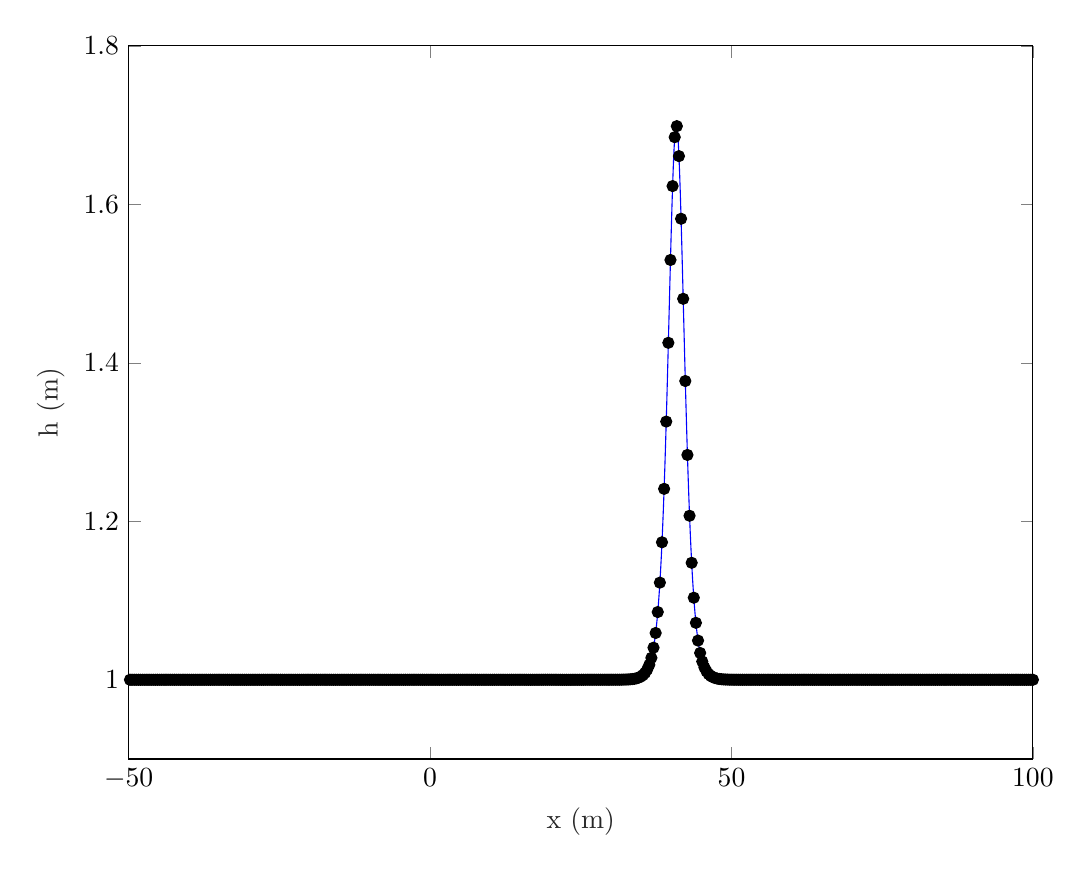
\begin{tikzpicture}

\begin{axis}[%
width=4.521in,
height=3.566in,
at={(0.758in,0.481in)},
scale only axis,
xmin=-50,
xmax=100,
xtick={-50,   0,  50, 100},
xlabel style={font=\color{white!15!black}},
xlabel={x (m)},
ymin=0.9,
ymax=1.8,
ytick={  1, 1.2, 1.4, 1.6, 1.8},
ylabel style={font=\color{white!15!black}},
ylabel={h (m)},
axis background/.style={fill=white}
]
\addplot [color=blue, forget plot]
  table[row sep=crcr]{%
-50.14064697609	1\\
-50.0234411626817	1\\
-49.9062353492733	1\\
-49.789029535865	1\\
-49.6718237224566	1\\
-49.5546179090483	1\\
-49.4374120956399	1\\
-49.3202062822316	1\\
-49.2030004688233	1\\
-49.0857946554149	1\\
-48.9685888420066	1\\
-48.8513830285982	1\\
-48.7341772151899	1\\
-48.6169714017815	1\\
-48.4997655883732	1\\
-48.3825597749648	1\\
-48.2653539615565	1\\
-48.1481481481481	1\\
-48.0309423347398	1\\
-47.9137365213315	1\\
-47.7965307079231	1\\
-47.6793248945148	1\\
-47.5621190811064	1\\
-47.4449132676981	1\\
-47.3277074542897	1\\
-47.2105016408814	1\\
-47.093295827473	1\\
-46.9760900140647	1\\
-46.8588842006564	1\\
-46.741678387248	1\\
-46.6244725738397	1\\
-46.5072667604313	1\\
-46.390060947023	1\\
-46.2728551336146	1\\
-46.1556493202063	1\\
-46.0384435067979	1\\
-45.9212376933896	1\\
-45.8040318799812	1\\
-45.6868260665729	1\\
-45.5696202531646	1\\
-45.4524144397562	1\\
-45.3352086263479	1\\
-45.2180028129395	1\\
-45.1007969995312	1\\
-44.9835911861228	1\\
-44.8663853727145	1\\
-44.7491795593061	1\\
-44.6319737458978	1\\
-44.5147679324894	1\\
-44.3975621190811	1\\
-44.2803563056728	1\\
-44.1631504922644	1\\
-44.0459446788561	1\\
-43.9287388654477	1\\
-43.8115330520394	1\\
-43.694327238631	1\\
-43.5771214252227	1\\
-43.4599156118143	1\\
-43.342709798406	1\\
-43.2255039849977	1\\
-43.1082981715893	1\\
-42.991092358181	1\\
-42.8738865447726	1\\
-42.7566807313643	1\\
-42.6394749179559	1\\
-42.5222691045476	1\\
-42.4050632911392	1\\
-42.2878574777309	1\\
-42.1706516643225	1\\
-42.0534458509142	1\\
-41.9362400375059	1\\
-41.8190342240975	1\\
-41.7018284106892	1\\
-41.5846225972808	1\\
-41.4674167838725	1\\
-41.3502109704641	1\\
-41.2330051570558	1\\
-41.1157993436474	1\\
-40.9985935302391	1\\
-40.8813877168308	1\\
-40.7641819034224	1\\
-40.6469760900141	1\\
-40.5297702766057	1\\
-40.4125644631974	1\\
-40.295358649789	1\\
-40.1781528363807	1\\
-40.0609470229723	1\\
-39.943741209564	1\\
-39.8265353961556	1\\
-39.7093295827473	1\\
-39.592123769339	1\\
-39.4749179559306	1\\
-39.3577121425223	1\\
-39.2405063291139	1\\
-39.1233005157056	1\\
-39.0060947022972	1\\
-38.8888888888889	1\\
-38.7716830754805	1\\
-38.6544772620722	1\\
-38.5372714486639	1\\
-38.4200656352555	1\\
-38.3028598218472	1\\
-38.1856540084388	1\\
-38.0684481950305	1\\
-37.9512423816221	1\\
-37.8340365682138	1\\
-37.7168307548054	1\\
-37.5996249413971	1\\
-37.4824191279887	1\\
-37.3652133145804	1\\
-37.2480075011721	1\\
-37.1308016877637	1\\
-37.0135958743554	1\\
-36.896390060947	1\\
-36.7791842475387	1\\
-36.6619784341303	1\\
-36.544772620722	1\\
-36.4275668073136	1\\
-36.3103609939053	1\\
-36.193155180497	1\\
-36.0759493670886	1\\
-35.9587435536803	1\\
-35.8415377402719	1\\
-35.7243319268636	1\\
-35.6071261134552	1\\
-35.4899203000469	1\\
-35.3727144866385	1\\
-35.2555086732302	1\\
-35.1383028598218	1\\
-35.0210970464135	1\\
-34.9038912330052	1\\
-34.7866854195968	1\\
-34.6694796061885	1\\
-34.5522737927801	1\\
-34.4350679793718	1\\
-34.3178621659634	1\\
-34.2006563525551	1\\
-34.0834505391467	1\\
-33.9662447257384	1\\
-33.8490389123301	1\\
-33.7318330989217	1\\
-33.6146272855134	1\\
-33.497421472105	1\\
-33.3802156586967	1\\
-33.2630098452883	1\\
-33.14580403188	1\\
-33.0285982184716	1\\
-32.9113924050633	1\\
-32.7941865916549	1\\
-32.6769807782466	1\\
-32.5597749648383	1\\
-32.4425691514299	1\\
-32.3253633380216	1\\
-32.2081575246132	1\\
-32.0909517112049	1\\
-31.9737458977965	1\\
-31.8565400843882	1\\
-31.7393342709798	1\\
-31.6221284575715	1\\
-31.5049226441632	1\\
-31.3877168307548	1\\
-31.2705110173465	1\\
-31.1533052039381	1\\
-31.0360993905298	1\\
-30.9188935771214	1\\
-30.8016877637131	1\\
-30.6844819503047	1\\
-30.5672761368964	1\\
-30.450070323488	1\\
-30.3328645100797	1\\
-30.2156586966714	1\\
-30.098452883263	1\\
-29.9812470698547	1\\
-29.8640412564463	1\\
-29.746835443038	1\\
-29.6296296296296	1\\
-29.5124238162213	1\\
-29.3952180028129	1\\
-29.2780121894046	1\\
-29.1608063759962	1\\
-29.0436005625879	1\\
-28.9263947491796	1\\
-28.8091889357712	1\\
-28.6919831223629	1\\
-28.5747773089545	1\\
-28.4575714955462	1\\
-28.3403656821378	1\\
-28.2231598687295	1\\
-28.1059540553211	1\\
-27.9887482419128	1\\
-27.8715424285045	1\\
-27.7543366150961	1\\
-27.6371308016878	1\\
-27.5199249882794	1\\
-27.4027191748711	1\\
-27.2855133614627	1\\
-27.1683075480544	1\\
-27.051101734646	1\\
-26.9338959212377	1\\
-26.8166901078293	1\\
-26.699484294421	1\\
-26.5822784810127	1\\
-26.4650726676043	1\\
-26.347866854196	1\\
-26.2306610407876	1\\
-26.1134552273793	1\\
-25.9962494139709	1\\
-25.8790436005626	1\\
-25.7618377871542	1\\
-25.6446319737459	1\\
-25.5274261603376	1\\
-25.4102203469292	1\\
-25.2930145335209	1\\
-25.1758087201125	1\\
-25.0586029067042	1\\
-24.9413970932958	1\\
-24.8241912798875	1\\
-24.7069854664791	1\\
-24.5897796530708	1\\
-24.4725738396624	1\\
-24.3553680262541	1\\
-24.2381622128458	1\\
-24.1209563994374	1\\
-24.0037505860291	1\\
-23.8865447726207	1\\
-23.7693389592124	1\\
-23.652133145804	1\\
-23.5349273323957	1\\
-23.4177215189873	1\\
-23.300515705579	1\\
-23.1833098921707	1\\
-23.0661040787623	1\\
-22.948898265354	1\\
-22.8316924519456	1\\
-22.7144866385373	1\\
-22.5972808251289	1\\
-22.4800750117206	1\\
-22.3628691983122	1\\
-22.2456633849039	1\\
-22.1284575714955	1\\
-22.0112517580872	1\\
-21.8940459446789	1\\
-21.7768401312705	1\\
-21.6596343178622	1\\
-21.5424285044538	1\\
-21.4252226910455	1\\
-21.3080168776371	1\\
-21.1908110642288	1\\
-21.0736052508204	1\\
-20.9563994374121	1\\
-20.8391936240038	1\\
-20.7219878105954	1\\
-20.6047819971871	1\\
-20.4875761837787	1\\
-20.3703703703704	1\\
-20.253164556962	1\\
-20.1359587435537	1\\
-20.0187529301453	1\\
-19.901547116737	1\\
-19.7843413033286	1\\
-19.6671354899203	1\\
-19.549929676512	1\\
-19.4327238631036	1\\
-19.3155180496953	1\\
-19.1983122362869	1\\
-19.0811064228786	1\\
-18.9639006094702	1\\
-18.8466947960619	1\\
-18.7294889826535	1\\
-18.6122831692452	1\\
-18.4950773558368	1\\
-18.3778715424285	1\\
-18.2606657290202	1\\
-18.1434599156118	1\\
-18.0262541022035	1\\
-17.9090482887951	1\\
-17.7918424753868	1\\
-17.6746366619784	1\\
-17.5574308485701	1\\
-17.4402250351617	1\\
-17.3230192217534	1\\
-17.2058134083451	1\\
-17.0886075949367	1\\
-16.9714017815284	1\\
-16.85419596812	1\\
-16.7369901547117	1\\
-16.6197843413033	1\\
-16.502578527895	1\\
-16.3853727144866	1\\
-16.2681669010783	1\\
-16.1509610876699	1\\
-16.0337552742616	1\\
-15.9165494608533	1\\
-15.7993436474449	1\\
-15.6821378340366	1\\
-15.5649320206282	1\\
-15.4477262072199	1\\
-15.3305203938115	1\\
-15.2133145804032	1\\
-15.0961087669948	1\\
-14.9789029535865	1\\
-14.8616971401782	1\\
-14.7444913267698	1\\
-14.6272855133615	1\\
-14.5100796999531	1\\
-14.3928738865448	1\\
-14.2756680731364	1\\
-14.1584622597281	1\\
-14.0412564463197	1\\
-13.9240506329114	1\\
-13.806844819503	1\\
-13.6896390060947	1\\
-13.5724331926864	1\\
-13.455227379278	1\\
-13.3380215658697	1\\
-13.2208157524613	1\\
-13.103609939053	1\\
-12.9864041256446	1\\
-12.8691983122363	1\\
-12.7519924988279	1\\
-12.6347866854196	1\\
-12.5175808720113	1\\
-12.4003750586029	1\\
-12.2831692451946	1\\
-12.1659634317862	1\\
-12.0487576183779	1\\
-11.9315518049695	1\\
-11.8143459915612	1\\
-11.6971401781528	1\\
-11.5799343647445	1\\
-11.4627285513361	1\\
-11.3455227379278	1\\
-11.2283169245195	1\\
-11.1111111111111	1\\
-10.9939052977028	1\\
-10.8766994842944	1\\
-10.7594936708861	1\\
-10.6422878574777	1\\
-10.5250820440694	1\\
-10.407876230661	1\\
-10.2906704172527	1\\
-10.1734646038444	1\\
-10.056258790436	1\\
-9.93905297702766	1\\
-9.82184716361932	1\\
-9.70464135021097	1\\
-9.58743553680262	1\\
-9.47022972339428	1\\
-9.35302390998594	1\\
-9.23581809657759	1\\
-9.11861228316924	1\\
-9.0014064697609	1\\
-8.88420065635255	1\\
-8.76699484294421	1\\
-8.64978902953587	1\\
-8.53258321612752	1\\
-8.41537740271917	1\\
-8.29817158931083	1\\
-8.18096577590249	1\\
-8.06375996249414	1\\
-7.94655414908579	1\\
-7.82934833567745	1\\
-7.7121425222691	1\\
-7.59493670886076	1\\
-7.47773089545242	1\\
-7.36052508204407	1\\
-7.24331926863572	1\\
-7.12611345522738	1\\
-7.00890764181904	1\\
-6.89170182841069	1\\
-6.77449601500234	1\\
-6.657290201594	1\\
-6.54008438818565	1\\
-6.42287857477731	1\\
-6.30567276136896	1\\
-6.18846694796062	1\\
-6.07126113455227	1\\
-5.95405532114393	1\\
-5.83684950773559	1\\
-5.71964369432724	1\\
-5.60243788091889	1\\
-5.48523206751055	1\\
-5.3680262541022	1\\
-5.25082044069386	1\\
-5.13361462728551	1\\
-5.01640881387717	1\\
-4.89920300046882	1\\
-4.78199718706048	1\\
-4.66479137365214	1\\
-4.54758556024379	1\\
-4.43037974683544	1\\
-4.31317393342709	1\\
-4.19596812001875	1\\
-4.07876230661041	1\\
-3.96155649320206	1\\
-3.84435067979372	1\\
-3.72714486638537	1\\
-3.60993905297703	1\\
-3.49273323956868	1\\
-3.37552742616034	1\\
-3.25832161275199	1\\
-3.14111579934364	1\\
-3.0239099859353	1\\
-2.90670417252696	1\\
-2.78949835911861	1\\
-2.67229254571027	1\\
-2.55508673230192	1\\
-2.43788091889358	1\\
-2.32067510548523	1\\
-2.20346929207689	1\\
-2.08626347866854	1\\
-1.96905766526019	1\\
-1.85185185185185	1\\
-1.73464603844351	1\\
-1.61744022503516	1\\
-1.50023441162681	1\\
-1.38302859821847	1\\
-1.26582278481013	1\\
-1.14861697140178	1\\
-1.03141115799344	1\\
-0.914205344585092	1\\
-0.796999531176745	1\\
-0.679793717768398	1\\
-0.562587904360058	1\\
-0.445382090951711	1\\
-0.328176277543363	1\\
-0.210970464135023	1\\
-0.0937646507266763	1\\
0.0234411626816708	1\\
0.140646976090011	1\\
0.257852789498358	1\\
0.375058602906705	1\\
0.492264416315052	1\\
0.609470229723392	1\\
0.726676043131739	1\\
0.843881856540087	1\\
0.961087669948427	1\\
1.07829348335677	1\\
1.19549929676512	1\\
1.31270511017347	1\\
1.42991092358181	1\\
1.54711673699016	1\\
1.6643225503985	1\\
1.78152836380684	1\\
1.89873417721519	1\\
2.01593999062354	1\\
2.13314580403188	1\\
2.25035161744022	1\\
2.36755743084857	1\\
2.48476324425692	1\\
2.60196905766526	1\\
2.71917487107361	1\\
2.83638068448195	1\\
2.95358649789029	1\\
3.07079231129864	1\\
3.18799812470699	1\\
3.30520393811533	1\\
3.42240975152367	1\\
3.53961556493202	1\\
3.65682137834037	1\\
3.77402719174871	1\\
3.89123300515705	1\\
4.0084388185654	1\\
4.12564463197375	1\\
4.24285044538209	1\\
4.36005625879044	1\\
4.47726207219878	1\\
4.59446788560712	1\\
4.71167369901547	1\\
4.82887951242382	1\\
4.94608532583216	1\\
5.0632911392405	1\\
5.18049695264885	1\\
5.2977027660572	1\\
5.41490857946554	1\\
5.53211439287389	1\\
5.64932020628223	1\\
5.76652601969058	1\\
5.88373183309892	1\\
6.00093764650727	1\\
6.11814345991561	1\\
6.23534927332395	1\\
6.3525550867323	1\\
6.46976090014065	1\\
6.58696671354899	1\\
6.70417252695734	1\\
6.82137834036568	1\\
6.93858415377403	1\\
7.05578996718237	1\\
7.17299578059072	1\\
7.29020159399906	1\\
7.4074074074074	1\\
7.52461322081575	1\\
7.6418190342241	1\\
7.75902484763245	1\\
7.87623066104079	1\\
7.99343647444913	1\\
8.11064228785748	1\\
8.22784810126582	1\\
8.34505391467417	1\\
8.46225972808251	1\\
8.57946554149086	1\\
8.6966713548992	1\\
8.81387716830755	1\\
8.9310829817159	1\\
9.04828879512424	1\\
9.16549460853258	1\\
9.28270042194093	1\\
9.39990623534927	1\\
9.51711204875762	1\\
9.63431786216596	1\\
9.75152367557431	1\\
9.86872948898265	1\\
9.985935302391	1\\
10.1031411157993	1\\
10.2203469292077	1\\
10.337552742616	1.00000000000001\\
10.4547585560244	1.00000000000001\\
10.5719643694327	1.00000000000001\\
10.6891701828411	1.00000000000001\\
10.8063759962494	1.00000000000001\\
10.9235818096578	1.00000000000001\\
11.0407876230661	1.00000000000001\\
11.1579934364744	1.00000000000001\\
11.2751992498828	1.00000000000001\\
11.3924050632911	1.00000000000002\\
11.5096108766995	1.00000000000002\\
11.6268166901078	1.00000000000002\\
11.7440225035162	1.00000000000003\\
11.8612283169245	1.00000000000003\\
11.9784341303329	1.00000000000003\\
12.0956399437412	1.00000000000004\\
12.2128457571496	1.00000000000004\\
12.3300515705579	1.00000000000005\\
12.4472573839662	1.00000000000005\\
12.5644631973746	1.00000000000006\\
12.6816690107829	1.00000000000007\\
12.7988748241913	1.00000000000008\\
12.9160806375996	1.00000000000009\\
13.033286451008	1.00000000000011\\
13.1504922644163	1.00000000000012\\
13.2676980778247	1.00000000000014\\
13.384903891233	1.00000000000016\\
13.5021097046413	1.00000000000018\\
13.6193155180497	1.0000000000002\\
13.736521331458	1.00000000000023\\
13.8537271448664	1.00000000000026\\
13.9709329582747	1.0000000000003\\
14.0881387716831	1.00000000000034\\
14.2053445850914	1.00000000000039\\
14.3225503984998	1.00000000000044\\
14.4397562119081	1.0000000000005\\
14.5569620253165	1.00000000000057\\
14.6741678387248	1.00000000000065\\
14.7913736521331	1.00000000000074\\
14.9085794655415	1.00000000000085\\
15.0257852789498	1.00000000000096\\
15.1429910923582	1.0000000000011\\
15.2601969057665	1.00000000000125\\
15.3774027191749	1.00000000000142\\
15.4946085325832	1.00000000000162\\
15.6118143459916	1.00000000000185\\
15.7290201593999	1.00000000000211\\
15.8462259728083	1.0000000000024\\
15.9634317862166	1.00000000000273\\
16.0806375996249	1.00000000000311\\
16.1978434130333	1.00000000000354\\
16.3150492264416	1.00000000000404\\
16.43225503985	1.0000000000046\\
16.5494608532583	1.00000000000524\\
16.6666666666667	1.00000000000597\\
16.783872480075	1.0000000000068\\
16.9010782934834	1.00000000000775\\
17.0182841068917	1.00000000000882\\
17.1354899203	1.00000000001005\\
17.2526957337084	1.00000000001145\\
17.3699015471167	1.00000000001304\\
17.4871073605251	1.00000000001486\\
17.6043131739334	1.00000000001692\\
17.7215189873418	1.00000000001928\\
17.8387248007501	1.00000000002196\\
17.9559306141585	1.00000000002502\\
18.0731364275668	1.0000000000285\\
18.1903422409752	1.00000000003246\\
18.3075480543835	1.00000000003698\\
18.4247538677918	1.00000000004212\\
18.5419596812002	1.00000000004798\\
18.6591654946085	1.00000000005466\\
18.7763713080169	1.00000000006226\\
18.8935771214252	1.00000000007093\\
19.0107829348336	1.00000000008079\\
19.1279887482419	1.00000000009204\\
19.2451945616503	1.00000000010484\\
19.3624003750586	1.00000000011943\\
19.4796061884669	1.00000000013604\\
19.5968120018753	1.00000000015497\\
19.7140178152836	1.00000000017653\\
19.831223628692	1.00000000020109\\
19.9484294421003	1.00000000022907\\
20.0656352555087	1.00000000026094\\
20.182841068917	1.00000000029725\\
20.3000468823254	1.00000000033861\\
20.4172526957337	1.00000000038572\\
20.5344585091421	1.00000000043938\\
20.6516643225504	1.00000000050052\\
20.7688701359587	1.00000000057015\\
20.8860759493671	1.00000000064948\\
21.0032817627754	1.00000000073985\\
21.1204875761838	1.00000000084278\\
21.2376933895921	1.00000000096004\\
21.3548992030005	1.00000000109361\\
21.4721050164088	1.00000000124577\\
21.5893108298172	1.0000000014191\\
21.7065166432255	1.00000000161654\\
21.8237224566338	1.00000000184145\\
21.9409282700422	1.00000000209766\\
22.0581340834505	1.00000000238951\\
22.1753398968589	1.00000000272197\\
22.2925457102672	1.00000000310068\\
22.4097515236756	1.00000000353209\\
22.5269573370839	1.00000000402352\\
22.6441631504923	1.00000000458332\\
22.7613689639006	1.00000000522101\\
22.878574777309	1.00000000594742\\
22.9957805907173	1.0000000067749\\
23.1129864041256	1.00000000771751\\
23.230192217534	1.00000000879126\\
23.3473980309423	1.00000001001441\\
23.4646038443507	1.00000001140774\\
23.581809657759	1.00000001299493\\
23.6990154711674	1.00000001480295\\
23.8162212845757	1.00000001686252\\
23.9334270979841	1.00000001920864\\
24.0506329113924	1.00000002188119\\
24.1678387248007	1.00000002492557\\
24.2850445382091	1.00000002839353\\
24.4022503516174	1.00000003234399\\
24.5194561650258	1.00000003684409\\
24.6366619784341	1.00000004197029\\
24.7538677918425	1.00000004780973\\
24.8710736052508	1.00000005446161\\
24.9882794186592	1.00000006203899\\
25.1054852320675	1.00000007067062\\
25.2226910454759	1.0000000805032\\
25.3398968588842	1.00000009170381\\
25.4571026722925	1.00000010446279\\
25.5743084857009	1.00000011899695\\
25.6915142991092	1.00000013555329\\
25.8087201125176	1.00000015441315\\
25.9259259259259	1.00000017589703\\
26.0431317393343	1.00000020037001\\
26.1603375527426	1.00000022824798\\
26.277543366151	1.00000026000468\\
26.3947491795593	1.00000029617977\\
26.5119549929676	1.00000033738798\\
26.629160806376	1.00000038432959\\
26.7463666197843	1.0000004378023\\
26.8635724331927	1.00000049871479\\
26.980778246601	1.00000056810218\\
27.0979840600094	1.0000006471436\\
27.2151898734177	1.00000073718224\\
27.3323956868261	1.00000083974816\\
27.4496015002344	1.00000095658431\\
27.5668073136428	1.00000108967614\\
27.6840131270511	1.00000124128534\\
27.8012189404594	1.00000141398825\\
27.9184247538678	1.0000016107197\\
28.0356305672761	1.00000183482281\\
28.1528363806845	1.00000209010585\\
28.2700421940928	1.00000238090694\\
28.3872480075012	1.00000271216775\\
28.5044538209095	1.00000308951751\\
28.6216596343179	1.00000351936862\\
28.7388654477262	1.00000400902566\\
28.8560712611346	1.00000456680947\\
28.9732770745429	1.00000520219857\\
29.0904828879512	1.00000592599023\\
29.2076887013596	1.00000675048389\\
29.3248945147679	1.0000076896902\\
29.4421003281763	1.00000875956908\\
29.5593061415846	1.00000997830084\\
29.676511954993	1.00001136659518\\
29.7937177684013	1.00001294804298\\
29.9109235818097	1.00001474951715\\
30.028129395218	1.00001680162923\\
30.1453352086263	1.00001913924939\\
30.2625410220347	1.00002180209889\\
30.379746835443	1.00002483542488\\
30.4969526488514	1.00002829076897\\
30.6141584622597	1.00003222684283\\
30.7313642756681	1.00003671052539\\
30.8485700890764	1.00004181799877\\
30.9657759024848	1.00004763604212\\
31.0829817158931	1.00005426350526\\
31.2001875293015	1.00006181298725\\
31.3173933427098	1.00007041274808\\
31.4345991561181	1.00008020888611\\
31.5518049695265	1.00009136781794\\
31.6690107829348	1.00010407910273\\
31.7862165963432	1.00011855865867\\
31.9034224097515	1.00013505242597\\
32.0206282231599	1.00015384053823\\
32.1378340365682	1.00017524207239\\
32.2550398499766	1.00019962045743\\
32.3722456633849	1.00022738963267\\
32.4894514767932	1.00025902105926\\
32.6066572902016	1.00029505170228\\
32.7238631036099	1.00033609311725\\
32.8410689170183	1.0003828417927\\
32.9582747304266	1.00043609092128\\
33.075480543835	1.00049674379492\\
33.1926863572433	1.00056582904603\\
33.3098921706517	1.00064451798632\\
33.42709798406	1.00073414432823\\
33.5443037974684	1.00083622661165\\
33.6615096108767	1.00095249370097\\
33.778715424285	1.0010849137646\\
33.8959212376934	1.00123572720247\\
34.0131270511017	1.00140748404565\\
34.1303328645101	1.00160308641825\\
34.2475386779184	1.00182583672379\\
34.3647444913268	1.00207949229868\\
34.4819503047351	1.00236832736205\\
34.5991561181435	1.00269720318669\\
34.7163619315518	1.00307164751712\\
34.8335677449601	1.00349794436982\\
34.9507735583685	1.00398323546349\\
35.0679793717768	1.00453563464401\\
35.1851851851852	1.00516435678464\\
35.3023909985935	1.00587986275291\\
35.4195968120019	1.00669402213515\\
35.5368026254102	1.00762029548797\\
35.6540084388186	1.00867393793132\\
35.7712142522269	1.00987222589332\\
35.8884200656353	1.0112347087405\\
36.0056258790436	1.01278348685073\\
36.122831692452	1.01454351737156\\
36.2400375058603	1.01654294840809\\
36.3572433192686	1.01881348163989\\
36.474449132677	1.02139076230266\\
36.5916549460853	1.02431479399257\\
36.7088607594937	1.02763037374657\\
36.826066572902	1.03138754018544\\
36.9432723863104	1.03564202401603\\
37.0604781997187	1.04045568569542\\
37.177684013127	1.04589691935839\\
37.2948898265354	1.05204099499315\\
37.4120956399437	1.05897030211297\\
37.5293014533521	1.06677444764938\\
37.6465072667604	1.07555014839734\\
37.7637130801688	1.08540084413538\\
37.8809188935771	1.09643594181754\\
37.9981247069855	1.10876958464425\\
38.1153305203938	1.12251882353235\\
38.2325363338022	1.13780105438818\\
38.3497421472105	1.15473057541087\\
38.4669479606189	1.17341411827757\\
38.5841537740272	1.1939452205691\\
38.7013595874355	1.21639734045667\\
38.8185654008439	1.24081567565857\\
38.9357712142522	1.26720774434257\\
39.0529770276606	1.2955329222128\\
39.1701828410689	1.32569131053987\\
39.2873886544773	1.35751253148912\\
39.4045944678856	1.390745297658\\
39.5218002812939	1.42504885763197\\
39.6390060947023	1.45998763933329\\
39.7562119081106	1.49503054446875\\
39.873417721519	1.52955632751224\\
39.9906235349273	1.56286625940054\\
40.1078293483357	1.59420478473859\\
40.225035161744	1.62278812430555\\
40.3422409751524	1.64783980054667\\
40.4594467885607	1.66863098727213\\
40.5766526019691	1.68452258078498\\
40.6938584153774	1.69500516570792\\
40.8110642287858	1.69973279861715\\
40.9282700421941	1.69854688081361\\
41.0454758556024	1.69148734707972\\
41.1626816690108	1.67878983410198\\
41.2798874824191	1.66086916888311\\
41.3970932958275	1.63829113257875\\
41.5142991092358	1.61173572291671\\
41.6315049226442	1.58195585851466\\
41.7487107360525	1.54973556893153\\
41.8659165494608	1.51585125455816\\
41.9831223628692	1.48103873924162\\
42.1003281762775	1.44596778161234\\
42.2175339896859	1.41122465757309\\
42.3347398030942	1.3773025291539\\
42.4519456165026	1.34459866185464\\
42.5691514299109	1.3134171679134\\
42.6863572433193	1.28397581179477\\
42.8035630567276	1.25641546268183\\
42.920768870136	1.23081095285464\\
43.0379746835443	1.20718234045221\\
43.1551804969527	1.18550583214261\\
43.272386310361	1.16572386238546\\
43.3895921237693	1.14775403199658\\
43.5067979371777	1.13149677160441\\
43.624003750586	1.11684171519414\\
43.7412095639944	1.10367284988357\\
43.8584153774027	1.09187255723844\\
43.9756211908111	1.08132468621399\\
44.0928270042194	1.07191680507409\\
44.2100328176277	1.06354177520369\\
44.3272386310361	1.05609877817921\\
44.4444444444444	1.04949391219976\\
44.5616502578528	1.04364045739367\\
44.6788560712611	1.03845889316303\\
44.7960618846695	1.033876735555\\
44.9132676980778	1.02982824914637\\
45.0304735114862	1.02625407628462\\
45.1476793248945	1.02310081673667\\
45.2648851383029	1.02032058273039\\
45.3820909517112	1.01787054784875\\
45.4992967651196	1.01571250304345\\
45.6165025785279	1.01381242896519\\
45.7337083919362	1.01214009066847\\
45.8509142053446	1.01066865836391\\
45.9681200187529	1.00937435611301\\
46.0853258321613	1.00823613906005\\
46.2025316455696	1.00723539886986\\
46.319737458978	1.00635569640231\\
46.4369432723863	1.0055825202356\\
46.5541490857947	1.0049030693964\\
46.671354899203	1.00430605852224\\
46.7885607126113	1.00378154363688\\
46.9057665260197	1.00332076673743\\
47.022972339428	1.0029160174518\\
47.1401781528364	1.00256051011353\\
47.2573839662447	1.00224827470599\\
47.3745897796531	1.00197406024124\\
47.4917955930614	1.00173324925606\\
47.6090014064698	1.00152178222268\\
47.7262072198781	1.00133609078359\\
47.8434130332865	1.00117303882565\\
47.9606188466948	1.00102987050806\\
48.0778246601031	1.00090416445011\\
48.1950304735115	1.00079379336951\\
48.3122362869198	1.0006968885386\\
48.4294421003282	1.00061180849548\\
48.5466479137365	1.00053711151023\\
48.6638537271449	1.00047153136275\\
48.7810595405532	1.00041395603937\\
48.8982653539616	1.00036340900106\\
49.0154711673699	1.00031903271587\\
49.1326769807782	1.0002800741846\\
49.2498827941866	1.00024587222034\\
49.3670886075949	1.00021584627088\\
49.4842944210033	1.00018948659805\\
49.6015002344116	1.00016634565013\\
49.71870604782	1.00014603048306\\
49.8359118612283	1.00012819610352\\
49.9531176746367	1.00011253962214\\
50.070323488045	1.00009879511859\\
50.1875293014534	1.00008672913208\\
50.3047351148617	1.00007613670128\\
50.42194092827	1.00006683788695\\
50.5391467416784	1.0000586747184\\
50.6563525550867	1.00005150851238\\
50.7735583684951	1.00004521751891\\
50.8907641819034	1.0000396948543\\
51.0079699953118	1.00003484668635\\
51.1251758087201	1.00003059064095\\
51.2423816221285	1.00002685440323\\
51.3595874355368	1.0000235744893\\
51.4767932489451	1.00002069516802\\
51.5939990623535	1.00001816751431\\
51.7112048757618	1.00001594857809\\
51.8284106891702	1.00001400065467\\
51.9456165025785	1.00001229064413\\
52.0628223159869	1.00001078948908\\
52.1800281293952	1.00000947168091\\
52.2972339428036	1.00000831482643\\
52.4144397562119	1.00000729926738\\
52.5316455696203	1.00000640774646\\
52.6488513830286	1.00000562511405\\
52.7660571964369	1.00000493807084\\
52.8832630098453	1.00000433494182\\
53.0004688232536	1.00000380547792\\
53.117674636662	1.00000334068188\\
53.2348804500703	1.00000293265529\\
53.3520862634787	1.00000257446445\\
53.469292076887	1.00000226002252\\
53.5864978902954	1.00000198398609\\
53.7037037037037	1.00000174166437\\
53.820909517112	1.00000152893951\\
53.9381153305204	1.00000134219659\\
54.0553211439287	1.00000117826222\\
54.1725269573371	1.00000103435059\\
54.2897327707454	1.00000090801616\\
54.4069385841538	1.00000079711206\\
54.5241443975621	1.00000069975366\\
54.6413502109705	1.00000061428651\\
54.7585560243788	1.00000053925822\\
54.8757618377872	1.0000004733938\\
54.9929676511955	1.00000041557398\\
55.1101734646038	1.00000036481622\\
55.2273792780122	1.00000032025795\\
55.3445850914205	1.00000028114198\\
55.4617909048289	1.0000002468036\\
55.5789967182372	1.00000021665926\\
55.6962025316456	1.00000019019673\\
55.8134083450539	1.0000001669663\\
55.9306141584623	1.00000014657321\\
56.0478199718706	1.00000012867091\\
56.165025785279	1.00000011295518\\
56.2822315986873	1.00000009915895\\
56.3994374120956	1.00000008704778\\
56.516643225504	1.00000007641585\\
56.6338490389123	1.0000000670825\\
56.7510548523207	1.00000005888911\\
56.868260665729	1.00000005169646\\
56.9854664791374	1.00000004538231\\
57.1026722925457	1.00000003983936\\
57.2198781059541	1.00000003497342\\
57.3370839193624	1.0000000307018\\
57.4542897327707	1.00000002695192\\
57.5714955461791	1.00000002366004\\
57.6887013595874	1.00000002077022\\
57.8059071729958	1.00000001823337\\
57.9231129864041	1.00000001600637\\
58.0403187998125	1.00000001405136\\
58.1575246132208	1.00000001233515\\
58.2747304266292	1.00000001082854\\
58.3919362400375	1.00000000950596\\
58.5091420534459	1.00000000834491\\
58.6263478668542	1.00000000732567\\
58.7435536802625	1.00000000643092\\
58.8607594936709	1.00000000564545\\
58.9779653070792	1.00000000495592\\
59.0951711204876	1.00000000435061\\
59.2123769338959	1.00000000381923\\
59.3295827473043	1.00000000335276\\
59.4467885607126	1.00000000294325\\
59.563994374121	1.00000000258377\\
59.6812001875293	1.00000000226819\\
59.7984060009376	1.00000000199116\\
59.915611814346	1.00000000174796\\
60.0328176277543	1.00000000153446\\
60.1500234411627	1.00000000134705\\
60.267229254571	1.00000000118252\\
60.3844350679794	1.00000000103809\\
60.5016408813877	1.0000000009113\\
60.6188466947961	1.00000000079999\\
60.7360525082044	1.00000000070228\\
60.8532583216128	1.00000000061651\\
60.9704641350211	1.00000000054121\\
61.0876699484294	1.0000000004751\\
61.2048757618378	1.00000000041708\\
61.3220815752461	1.00000000036613\\
61.4392873886545	1.00000000032141\\
61.5564932020628	1.00000000028216\\
61.6736990154712	1.00000000024769\\
61.7909048288795	1.00000000021744\\
61.9081106422879	1.00000000019088\\
62.0253164556962	1.00000000016757\\
62.1425222691045	1.0000000001471\\
62.2597280825129	1.00000000012914\\
62.3769338959212	1.00000000011336\\
62.4941397093296	1.00000000009952\\
62.6113455227379	1.00000000008736\\
62.7285513361463	1.00000000007669\\
62.8457571495546	1.00000000006732\\
62.962962962963	1.0000000000591\\
63.0801687763713	1.00000000005188\\
63.1973745897797	1.00000000004555\\
63.314580403188	1.00000000003998\\
63.4317862165964	1.0000000000351\\
63.5489920300047	1.00000000003081\\
63.666197843413	1.00000000002705\\
63.7834036568214	1.00000000002375\\
63.9006094702297	1.00000000002085\\
64.0178152836381	1.0000000000183\\
64.1350210970464	1.00000000001606\\
64.2522269104548	1.0000000000141\\
64.3694327238631	1.00000000001238\\
64.4866385372714	1.00000000001087\\
64.6038443506798	1.00000000000954\\
64.7210501640881	1.00000000000838\\
64.8382559774965	1.00000000000735\\
64.9554617909048	1.00000000000645\\
65.0726676043132	1.00000000000567\\
65.1898734177215	1.00000000000497\\
65.3070792311299	1.00000000000437\\
65.4242850445382	1.00000000000383\\
65.5414908579466	1.00000000000336\\
65.6586966713549	1.00000000000295\\
65.7759024847633	1.00000000000259\\
65.8931082981716	1.00000000000228\\
66.0103141115799	1.000000000002\\
66.1275199249883	1.00000000000175\\
66.2447257383966	1.00000000000154\\
66.361931551805	1.00000000000135\\
66.4791373652133	1.00000000000119\\
66.5963431786217	1.00000000000104\\
66.71354899203	1.00000000000091\\
66.8307548054383	1.0000000000008\\
66.9479606188467	1.0000000000007\\
67.065166432255	1.00000000000062\\
67.1823722456634	1.00000000000054\\
67.2995780590717	1.00000000000048\\
67.4167838724801	1.00000000000042\\
67.5339896858884	1.00000000000037\\
67.6511954992968	1.00000000000032\\
67.7684013127051	1.00000000000028\\
67.8856071261135	1.00000000000025\\
68.0028129395218	1.00000000000022\\
68.1200187529302	1.00000000000019\\
68.2372245663385	1.00000000000017\\
68.3544303797468	1.00000000000015\\
68.4716361931552	1.00000000000013\\
68.5888420065635	1.00000000000011\\
68.7060478199719	1.0000000000001\\
68.8232536333802	1.00000000000009\\
68.9404594467886	1.00000000000008\\
69.0576652601969	1.00000000000007\\
69.1748710736052	1.00000000000006\\
69.2920768870136	1.00000000000005\\
69.4092827004219	1.00000000000005\\
69.5264885138303	1.00000000000004\\
69.6436943272386	1.00000000000004\\
69.760900140647	1.00000000000003\\
69.8781059540553	1.00000000000003\\
69.9953117674637	1.00000000000002\\
70.112517580872	1.00000000000002\\
70.2297233942804	1.00000000000002\\
70.3469292076887	1.00000000000002\\
70.4641350210971	1.00000000000001\\
70.5813408345054	1.00000000000001\\
70.6985466479137	1.00000000000001\\
70.8157524613221	1.00000000000001\\
70.9329582747304	1.00000000000001\\
71.0501640881388	1.00000000000001\\
71.1673699015471	1.00000000000001\\
71.2845757149555	1.00000000000001\\
71.4017815283638	1\\
71.5189873417721	1\\
71.6361931551805	1\\
71.7533989685888	1\\
71.8706047819972	1\\
71.9878105954055	1\\
72.1050164088139	1\\
72.2222222222222	1\\
72.3394280356306	1\\
72.4566338490389	1\\
72.5738396624473	1\\
72.6910454758556	1\\
72.8082512892639	1\\
72.9254571026723	1\\
73.0426629160806	1\\
73.159868729489	1\\
73.2770745428973	1\\
73.3942803563057	1\\
73.511486169714	1\\
73.6286919831224	1\\
73.7458977965307	1\\
73.8631036099391	1\\
73.9803094233474	1\\
74.0975152367557	1\\
74.2147210501641	1\\
74.3319268635724	1\\
74.4491326769808	1\\
74.5663384903891	1\\
74.6835443037975	1\\
74.8007501172058	1\\
74.9179559306142	1\\
75.0351617440225	1\\
75.1523675574308	1\\
75.2695733708392	1\\
75.3867791842475	1\\
75.5039849976559	1\\
75.6211908110642	1\\
75.7383966244726	1\\
75.8556024378809	1\\
75.9728082512893	1\\
76.0900140646976	1\\
76.207219878106	1\\
76.3244256915143	1\\
76.4416315049226	1\\
76.558837318331	1\\
76.6760431317393	1\\
76.7932489451477	1\\
76.910454758556	1\\
77.0276605719644	1\\
77.1448663853727	1\\
77.2620721987811	1\\
77.3792780121894	1\\
77.4964838255977	1\\
77.6136896390061	1\\
77.7308954524144	1\\
77.8481012658228	1\\
77.9653070792311	1\\
78.0825128926395	1\\
78.1997187060478	1\\
78.3169245194562	1\\
78.4341303328645	1\\
78.5513361462729	1\\
78.6685419596812	1\\
78.7857477730896	1\\
78.9029535864979	1\\
79.0201593999062	1\\
79.1373652133146	1\\
79.2545710267229	1\\
79.3717768401313	1\\
79.4889826535396	1\\
79.606188466948	1\\
79.7233942803563	1\\
79.8406000937647	1\\
79.957805907173	1\\
80.0750117205813	1\\
80.1922175339897	1\\
80.309423347398	1\\
80.4266291608064	1\\
80.5438349742147	1\\
80.6610407876231	1\\
80.7782466010314	1\\
80.8954524144397	1\\
81.0126582278481	1\\
81.1298640412564	1\\
81.2470698546648	1\\
81.3642756680731	1\\
81.4814814814815	1\\
81.5986872948898	1\\
81.7158931082982	1\\
81.8330989217065	1\\
81.9503047351149	1\\
82.0675105485232	1\\
82.1847163619315	1\\
82.3019221753399	1\\
82.4191279887482	1\\
82.5363338021566	1\\
82.6535396155649	1\\
82.7707454289733	1\\
82.8879512423816	1\\
83.00515705579	1\\
83.1223628691983	1\\
83.2395686826067	1\\
83.356774496015	1\\
83.4739803094234	1\\
83.5911861228317	1\\
83.70839193624	1\\
83.8255977496484	1\\
83.9428035630567	1\\
84.0600093764651	1\\
84.1772151898734	1\\
84.2944210032818	1\\
84.4116268166901	1\\
84.5288326300985	1\\
84.6460384435068	1\\
84.7632442569152	1\\
84.8804500703235	1\\
84.9976558837318	1\\
85.1148616971402	1\\
85.2320675105485	1\\
85.3492733239569	1\\
85.4664791373652	1\\
85.5836849507735	1\\
85.7008907641819	1\\
85.8180965775902	1\\
85.9353023909986	1\\
86.0525082044069	1\\
86.1697140178153	1\\
86.2869198312236	1\\
86.404125644632	1\\
86.5213314580403	1\\
86.6385372714487	1\\
86.755743084857	1\\
86.8729488982653	1\\
86.9901547116737	1\\
87.107360525082	1\\
87.2245663384904	1\\
87.3417721518987	1\\
87.4589779653071	1\\
87.5761837787154	1\\
87.6933895921238	1\\
87.8105954055321	1\\
87.9278012189405	1\\
88.0450070323488	1\\
88.1622128457572	1\\
88.2794186591655	1\\
88.3966244725738	1\\
88.5138302859822	1\\
88.6310360993905	1\\
88.7482419127989	1\\
88.8654477262072	1\\
88.9826535396156	1\\
89.0998593530239	1\\
89.2170651664323	1\\
89.3342709798406	1\\
89.451476793249	1\\
89.5686826066573	1\\
89.6858884200656	1\\
89.803094233474	1\\
89.9203000468823	1\\
90.0375058602907	1\\
90.154711673699	1\\
90.2719174871074	1\\
90.3891233005157	1\\
90.506329113924	1\\
90.6235349273324	1\\
90.7407407407407	1\\
90.8579465541491	1\\
90.9751523675574	1\\
91.0923581809658	1\\
91.2095639943741	1\\
91.3267698077825	1\\
91.4439756211908	1\\
91.5611814345991	1\\
91.6783872480075	1\\
91.7955930614158	1\\
91.9127988748242	1\\
92.0300046882325	1\\
92.1472105016409	1\\
92.2644163150492	1\\
92.3816221284576	1\\
92.4988279418659	1\\
92.6160337552743	1\\
92.7332395686826	1\\
92.850445382091	1\\
92.9676511954993	1\\
93.0848570089076	1\\
93.202062822316	1\\
93.3192686357243	1\\
93.4364744491327	1\\
93.553680262541	1\\
93.6708860759494	1\\
93.7880918893577	1\\
93.9052977027661	1\\
94.0225035161744	1\\
94.1397093295828	1\\
94.2569151429911	1\\
94.3741209563995	1\\
94.4913267698078	1\\
94.6085325832161	1\\
94.7257383966245	1\\
94.8429442100328	1\\
94.9601500234412	1\\
95.0773558368495	1\\
95.1945616502579	1\\
95.3117674636662	1\\
95.4289732770745	1\\
95.5461790904829	1\\
95.6633849038912	1\\
95.7805907172996	1\\
95.8977965307079	1\\
96.0150023441163	1\\
96.1322081575246	1\\
96.2494139709329	1\\
96.3666197843413	1\\
96.4838255977496	1\\
96.601031411158	1\\
96.7182372245663	1\\
96.8354430379747	1\\
96.952648851383	1\\
97.0698546647914	1\\
97.1870604781997	1\\
97.3042662916081	1\\
97.4214721050164	1\\
97.5386779184248	1\\
97.6558837318331	1\\
97.7730895452414	1\\
97.8902953586498	1\\
98.0075011720581	1\\
98.1247069854665	1\\
98.2419127988748	1\\
98.3591186122832	1\\
98.4763244256915	1\\
98.5935302390999	1\\
98.7107360525082	1\\
98.8279418659166	1\\
98.9451476793249	1\\
99.0623534927333	1\\
99.1795593061416	1\\
99.2967651195499	1\\
99.4139709329583	1\\
99.5311767463666	1\\
99.648382559775	1\\
99.7655883731833	1\\
99.8827941865917	1\\
100	1\\
100.117205813408	1\\
};
\addplot [color=black, draw=none, mark=*, mark options={solid, black}, forget plot]
  table[row sep=crcr]{%
-50.14064697609	1\\
-49.789029535865	0.999999999844261\\
-49.4374120956399	0.999999999827231\\
-49.0857946554149	0.999999999796034\\
-48.7341772151899	0.999999999748626\\
-48.3825597749648	0.999999999681601\\
-48.0309423347398	0.999999999590216\\
-47.6793248945148	0.999999999468107\\
-47.3277074542897	0.999999999306914\\
-46.9760900140647	0.999999999095814\\
-46.6244725738397	0.999999998820929\\
-46.2728551336146	0.999999998464581\\
-45.9212376933896	0.999999998004385\\
-45.5696202531646	0.999999997412137\\
-45.2180028129395	0.999999996652469\\
-44.8663853727145	0.999999995681228\\
-44.5147679324894	0.999999994443544\\
-44.1631504922644	0.999999992871542\\
-43.8115330520394	0.999999990881667\\
-43.4599156118143	0.999999988371558\\
-43.1082981715893	0.999999985216475\\
-42.7566807313643	0.99999998126521\\
-42.4050632911392	0.999999976335528\\
-42.0534458509142	0.999999970209118\\
-41.7018284106892	0.999999962626107\\
-41.3502109704641	0.999999953279263\\
-40.9985935302391	0.999999941807985\\
-40.6469760900141	0.999999927792351\\
-40.295358649789	0.999999910747482\\
-39.943741209564	0.999999890118667\\
-39.592123769339	0.999999865277712\\
-39.2405063291139	0.999999835521219\\
-38.8888888888889	0.999999800071523\\
-38.5372714486639	0.999999758081219\\
-38.1856540084388	0.999999708642346\\
-37.8340365682138	0.999999650801342\\
-37.4824191279887	0.999999583581019\\
-37.1308016877637	0.999999506010797\\
-36.7791842475387	0.999999417166307\\
-36.4275668073136	0.999999316219365\\
-36.0759493670886	0.999999202498896\\
-35.7243319268636	0.999999075562894\\
-35.3727144866385	0.999998935280731\\
-35.0210970464135	0.999998781924174\\
-34.6694796061885	0.999998616264192\\
-34.3178621659634	0.99999843966917\\
-33.9662447257384	0.999998254198431\\
-33.6146272855134	0.999998062683138\\
-33.2630098452883	0.99999786878478\\
-32.9113924050633	0.999997677019723\\
-32.5597749648383	0.999997492736927\\
-32.2081575246132	0.999997322035265\\
-31.8565400843882	0.999997171607101\\
-31.5049226441632	0.999997048496452\\
-31.1533052039381	0.999996959763415\\
-30.8016877637131	0.99999691205206\\
-30.450070323488	0.999996911067835\\
-30.098452883263	0.999996960972636\\
-29.746835443038	0.999997063742006\\
-29.3952180028129	0.999997218504692\\
-29.0436005625879	0.9999974209375\\
-28.6919831223629	0.999997662780163\\
-28.3403656821378	0.999997931555147\\
-27.9887482419128	0.999998210582851\\
-27.6371308016878	0.999998479381916\\
-27.2855133614627	0.999998714532948\\
-26.9338959212377	0.99999889105894\\
-26.5822784810127	0.999998984335573\\
-26.2306610407876	0.999998972483198\\
-25.8790436005626	0.999998839141072\\
-25.5274261603376	0.999998576395104\\
-25.1758087201125	0.999998187600579\\
-24.8241912798875	0.999997689725902\\
-24.4725738396624	0.999997114789484\\
-24.1209563994374	0.999996509948421\\
-23.7693389592124	0.999995935827789\\
-23.4177215189873	0.999995462785502\\
-23.0661040787623	0.999995164995744\\
-22.7144866385373	0.999995112512758\\
-22.3628691983122	0.99999536176526\\
-22.0112517580872	0.999995945478838\\
-21.6596343178622	0.999996863116711\\
-21.3080168776371	0.999998073544087\\
-20.9563994374121	0.999999491540687\\
-20.6047819971871	1.00000098979359\\
-20.253164556962	1.00000240757633\\
-19.901547116737	1.00000356655718\\
-19.549929676512	1.00000429307849\\
-19.1983122362869	1.00000444488842\\
-18.8466947960619	1.00000393915096\\
-18.4950773558368	1.0000027764976\\
-18.1434599156118	1.00000105677706\\
-17.7918424753868	0.99999898051179\\
-17.4402250351617	0.999996832770327\\
-17.0886075949367	0.999994947973813\\
-16.7369901547117	0.999993658128923\\
-16.3853727144866	0.999993231749326\\
-16.0337552742616	0.999993809118349\\
-15.6821378340366	0.999995362328081\\
-15.3305203938115	0.99999766890137\\
-14.9789029535865	1.00000033441108\\
-14.6272855133615	1.00000285315611\\
-14.2756680731364	1.00000470595287\\
-13.9240506329114	1.00000547890152\\
-13.5724331926864	1.00000496616556\\
-13.2208157524613	1.00000325813706\\
-12.8691983122363	1.00000073394252\\
-12.5175808720113	0.999997998262578\\
-12.1659634317862	0.999995736903251\\
-11.8143459915612	0.99999453301259\\
-11.4627285513361	0.999994693357057\\
-11.1111111111111	0.999996141491878\\
-10.7594936708861	0.999998423917342\\
-10.407876230661	1.00000083997314\\
-10.056258790436	1.00000266404459\\
-9.70464135021097	1.0000033885745\\
-9.35302390998594	1.00000288828638\\
-9.0014064697609	1.0000014624114\\
-8.64978902953587	0.999999690225684\\
-8.29817158931083	0.999998200642185\\
-7.94655414908579	0.999997432049661\\
-7.59493670886076	0.99999749889278\\
-7.24331926863572	0.999998213721819\\
-6.89170182841069	0.999999228947597\\
-6.54008438818565	1.00000019922371\\
-6.18846694796062	1.0000008730918\\
-5.83684950773559	1.00000110347455\\
-5.48523206751055	1.00000084063719\\
-5.13361462728551	1.00000016467835\\
-4.78199718706048	0.999999335489646\\
-4.43037974683544	0.999998737044713\\
-4.07876230661041	0.999998671923697\\
-3.72714486638537	0.99999913781774\\
-3.37552742616034	0.99999981181892\\
-3.0239099859353	1.00000029182737\\
-2.67229254571027	1.00000037631665\\
-2.32067510548523	1.00000014439204\\
-1.96905766526019	0.999999796953415\\
-1.61744022503516	0.999999490000687\\
-1.26582278481013	0.999999298210838\\
-0.914205344585092	0.999999353928455\\
-0.562587904360058	0.999999806148629\\
-0.210970464135023	1.00000032191158\\
0.140646976090011	0.999999945407871\\
0.492264416315052	0.999999172412708\\
0.843881856540087	1.00000022643642\\
1.19549929676512	0.999999784598468\\
1.54711673699016	0.999998587929371\\
1.89873417721519	1.00000077378411\\
2.25035161744022	1.0000022815906\\
2.60196905766526	0.999996638311547\\
2.95358649789029	0.999998272839358\\
3.30520393811533	1.00000134397295\\
3.65682137834037	1.00000117708053\\
4.0084388185654	0.999999520312057\\
4.36005625879044	0.999999256765235\\
4.71167369901547	1.00000035907299\\
5.0632911392405	1.00000083967979\\
5.41490857946554	0.999999559348049\\
5.76652601969058	0.999997487996241\\
6.11814345991561	0.999996653655047\\
6.46976090014065	0.999998339187713\\
6.82137834036568	1.00000195049882\\
7.17299578059072	1.00000532319706\\
7.52461322081575	1.00000600925323\\
7.87623066104079	1.00000284691821\\
8.22784810126582	0.999996880555951\\
8.57946554149086	0.999991044126855\\
8.9310829817159	0.999988683818313\\
9.28270042194093	0.999991726750406\\
9.63431786216596	0.999999479801298\\
9.985935302391	1.0000088081339\\
10.337552742616	1.00001552902188\\
10.6891701828411	1.00001633841085\\
11.0407876230661	1.00001031329398\\
11.3924050632911	0.999999334197621\\
11.7440225035162	0.999987312932316\\
12.0956399437412	0.999978648157976\\
12.4472573839662	0.99997658456668\\
12.7988748241913	0.999982107130394\\
13.1504922644163	0.99999369266571\\
13.5021097046413	1.00000792754191\\
13.8537271448664	1.00002065989371\\
14.2053445850914	1.00002826888208\\
14.5569620253165	1.00002865101562\\
14.9085794655415	1.00002167872425\\
15.2601969057665	1.00000908442002\\
15.6118143459916	0.999993878920453\\
15.9634317862166	0.999979529346799\\
16.3150492264416	0.999969131154066\\
16.6666666666667	0.999964772781617\\
17.0182841068917	0.999967184310295\\
17.3699015471167	0.999975755355418\\
17.7215189873418	0.999988764300763\\
18.0731364275668	1.000003827081\\
18.4247538677918	1.0000183865382\\
18.7763713080169	1.00003016284659\\
19.1279887482419	1.00003748934057\\
19.4796061884669	1.00003950175191\\
19.831223628692	1.00003614440605\\
20.182841068917	1.00002811874219\\
20.5344585091421	1.00001664759509\\
20.8860759493671	1.00000326523819\\
21.2376933895921	0.999989578212392\\
21.5893108298172	0.999977062931426\\
21.9409282700422	0.999966914462344\\
22.2925457102672	0.999959956488857\\
22.6441631504923	0.99995661066258\\
22.9957805907173	0.999956916440564\\
23.3473980309423	0.99996058911706\\
23.6990154711674	0.999967099198743\\
24.0506329113924	0.99997576194162\\
24.4022503516174	0.999985823644913\\
24.7538677918425	0.999996537181054\\
25.1054852320675	1.0000072215873\\
25.4571026722925	1.00001730366575\\
25.8087201125176	1.00002634193337\\
26.1603375527426	1.00003403520056\\
26.5119549929676	1.00004021848968\\
26.8635724331927	1.00004485076311\\
27.2151898734177	1.00004799734723\\
27.5668073136428	1.00004981100894\\
27.9184247538678	1.00005051498414\\
28.2700421940928	1.00005038983796\\
28.6216596343179	1.00004976761694\\
28.9732770745429	1.00004903553369\\
29.3248945147679	1.00004865224547\\
29.676511954993	1.00004917909486\\
30.028129395218	1.00005133813329\\
30.379746835443	1.00005609535749\\
30.7313642756681	1.00006479251442\\
31.0829817158931	1.00007934080048\\
31.4345991561181	1.0001025077037\\
31.7862165963432	1.00013834011503\\
32.1378340365682	1.00019278806947\\
32.4894514767932	1.00027462429216\\
32.8410689170183	1.00039679996504\\
33.1926863572433	1.00057844339669\\
33.5443037974684	1.00084780497437\\
33.8959212376934	1.00124659203359\\
34.2475386779184	1.00183633883077\\
34.5991561181435	1.00270774224161\\
34.9507735583685	1.00399428871063\\
35.3023909985935	1.00589202342771\\
35.6540084388186	1.00868796439034\\
36.0056258790436	1.01280036146538\\
36.3572433192686	1.01883447375186\\
36.7088607594937	1.02765709157233\\
37.0604781997187	1.04049008707179\\
37.4120956399437	1.05901461834177\\
37.7637130801688	1.08545737714747\\
38.1153305203938	1.12258965669411\\
38.4669479606189	1.17350099316541\\
38.8185654008439	1.24092052829898\\
39.1701828410689	1.32581763038889\\
39.5218002812939	1.42520212521207\\
39.873417721519	1.52973889166606\\
40.225035161744	1.62298539132868\\
40.5766526019691	1.68468969831869\\
40.9282700421941	1.69864255425566\\
41.2798874824191	1.66079424875662\\
41.6315049226442	1.58174124675909\\
41.9831223628692	1.48074249160056\\
42.3347398030942	1.37699422227331\\
42.6863572433193	1.28370433124302\\
43.0379746835443	1.20696780263092\\
43.3895921237693	1.1475960009455\\
43.7412095639944	1.10356150548863\\
44.0928270042194	1.0718404609216\\
44.4444444444444	1.04944240754197\\
44.7960618846695	1.03384231763793\\
45.1476793248945	1.02307794592182\\
45.4992967651196	1.01569735720297\\
45.8509142053446	1.01065865033152\\
46.2025316455696	1.00722879595257\\
46.5541490857947	1.00489871819597\\
46.9057665260197	1.0033179022432\\
47.2573839662447	1.00224639066722\\
47.6090014064698	1.0015205441454\\
47.9606188466948	1.00102905763988\\
48.3122362869198	1.00069635533124\\
48.6638537271449	1.00047118193394\\
49.0154711673699	1.00031880395269\\
49.3670886075949	1.00021569666357\\
49.71870604782	1.00014593275268\\
50.070323488045	1.00009873135337\\
50.42194092827	1.00006679633618\\
50.7735583684951	1.00004519048089\\
51.1251758087201	1.0000305730728\\
51.4767932489451	1.00002068377124\\
51.8284106891702	1.00001399327415\\
52.1800281293952	1.00000946691029\\
52.5316455696203	1.00000640466912\\
52.8832630098453	1.00000433296117\\
53.2348804500703	1.00000293138363\\
53.5864978902954	1.00000198317183\\
53.9381153305204	1.00000134167678\\
54.2897327707454	1.00000090768542\\
54.6413502109705	1.00000061407686\\
54.9929676511955	1.00000041544166\\
55.3445850914205	1.00000028105886\\
55.6962025316456	1.00000019014481\\
56.0478199718706	1.00000012863869\\
56.3994374120956	1.00000008702793\\
56.7510548523207	1.000000058877\\
57.1026722925457	1.00000003983205\\
57.4542897327707	1.00000002694757\\
57.8059071729958	1.00000001823083\\
58.1575246132208	1.00000001233369\\
58.5091420534459	1.00000000834411\\
58.8607594936709	1.00000000564504\\
59.2123769338959	1.00000000381903\\
59.563994374121	1.00000000258369\\
59.915611814346	1.00000000174794\\
60.267229254571	1.00000000118253\\
60.6188466947961	1.00000000080002\\
60.9704641350211	1.00000000054124\\
61.3220815752461	1.00000000036616\\
61.6736990154712	1.00000000024772\\
62.0253164556962	1.00000000016759\\
62.3769338959212	1.00000000011338\\
62.7285513361463	1.0000000000767\\
63.0801687763713	1.00000000005189\\
63.4317862165964	1.0000000000351\\
63.7834036568214	1.00000000002375\\
64.1350210970464	1.00000000001606\\
64.4866385372714	1.00000000001087\\
64.8382559774965	1.00000000000735\\
65.1898734177215	1.00000000000497\\
65.5414908579466	1.00000000000336\\
65.8931082981716	1.00000000000227\\
66.2447257383966	1.00000000000153\\
66.5963431786217	1.00000000000103\\
66.9479606188467	1.0000000000007\\
67.2995780590717	1.00000000000047\\
67.6511954992968	1.00000000000031\\
68.0028129395218	1.00000000000021\\
68.3544303797468	1.00000000000014\\
68.7060478199719	1.00000000000009\\
69.0576652601969	1.00000000000006\\
69.4092827004219	1.00000000000003\\
69.760900140647	1.00000000000002\\
70.112517580872	1.00000000000001\\
70.4641350210971	1\\
70.8157524613221	1\\
71.1673699015471	1\\
71.5189873417721	1\\
71.8706047819972	1\\
72.2222222222222	1\\
72.5738396624473	1\\
72.9254571026723	1\\
73.2770745428973	1\\
73.6286919831224	1\\
73.9803094233474	1\\
74.3319268635724	1\\
74.6835443037975	1\\
75.0351617440225	1\\
75.3867791842475	1\\
75.7383966244726	1\\
76.0900140646976	1\\
76.4416315049226	1\\
76.7932489451477	1\\
77.1448663853727	1\\
77.4964838255977	1\\
77.8481012658228	1\\
78.1997187060478	1\\
78.5513361462729	1\\
78.9029535864979	1\\
79.2545710267229	1\\
79.606188466948	1\\
79.957805907173	1\\
80.309423347398	1\\
80.6610407876231	1\\
81.0126582278481	1\\
81.3642756680731	1\\
81.7158931082982	1\\
82.0675105485232	1\\
82.4191279887482	1\\
82.7707454289733	1\\
83.1223628691983	1\\
83.4739803094234	1\\
83.8255977496484	1\\
84.1772151898734	1\\
84.5288326300985	1\\
84.8804500703235	1\\
85.2320675105485	1\\
85.5836849507735	1\\
85.9353023909986	1\\
86.2869198312236	1\\
86.6385372714487	1\\
86.9901547116737	1\\
87.3417721518987	1\\
87.6933895921238	1\\
88.0450070323488	1\\
88.3966244725738	1\\
88.7482419127989	1\\
89.0998593530239	1\\
89.451476793249	1\\
89.803094233474	1\\
90.154711673699	1\\
90.506329113924	1\\
90.8579465541491	1\\
91.2095639943741	1\\
91.5611814345991	1\\
91.9127988748242	1\\
92.2644163150492	1\\
92.6160337552743	1\\
92.9676511954993	1\\
93.3192686357243	1\\
93.6708860759494	1\\
94.0225035161744	1\\
94.3741209563995	1\\
94.7257383966245	1\\
95.0773558368495	1\\
95.4289732770745	1\\
95.7805907172996	1\\
96.1322081575246	1\\
96.4838255977496	1\\
96.8354430379747	1\\
97.1870604781997	1\\
97.5386779184248	1\\
97.8902953586498	1\\
98.2419127988748	1\\
98.5935302390999	1\\
98.9451476793249	1\\
99.2967651195499	1\\
99.648382559775	1\\
100	1\\
};
\end{axis}
\end{tikzpicture}%
		\caption{$t = 10s$}
	\end{subfigure}
	\begin{subfigure}{0.49\textwidth}
		\centering
		% This file was created by matlab2tikz.
%
%The latest updates can be retrieved from
%  http://www.mathworks.com/matlabcentral/fileexchange/22022-matlab2tikz-matlab2tikz
%where you can also make suggestions and rate matlab2tikz.
%
\begin{tikzpicture}

\begin{axis}[%
width=4.521in,
height=3.566in,
at={(0.758in,0.481in)},
scale only axis,
xmin=-50,
xmax=100,
xtick={-50,   0,  50, 100},
xlabel style={font=\color{white!15!black}},
xlabel={x (m)},
ymin=-0.1,
ymax=0.4,
ytick={-0.1,    0,  0.1,  0.2,  0.3,  0.4},
ylabel style={font=\color{white!15!black}},
ylabel={u (m/s)},
axis background/.style={fill=white}
]
\addplot [color=red, forget plot]
  table[row sep=crcr]{%
-50.2813379180994	1.06511867902256e-28\\
-50.0468896530166	1.91770795785705e-28\\
-49.8124413879337	3.44328815498068e-28\\
-49.5779931228509	6.16553397781048e-28\\
-49.3435448577681	1.10096737841321e-27\\
-49.1090965926852	1.96058030376556e-27\\
-48.8746483276024	3.48177937527298e-27\\
-48.6402000625195	6.16629488984274e-27\\
-48.4057517974367	1.08906489837559e-26\\
-48.1713035323539	1.91818133035259e-26\\
-47.936855267271	3.36924030658023e-26\\
-47.7024070021882	5.90174912275146e-26\\
-47.4679587371053	1.03094602732762e-25\\
-47.2335104720225	1.7959636544979e-25\\
-46.9990622069397	3.12007896947607e-25\\
-46.7646139418568	5.40555210117238e-25\\
-46.530165676774	9.33944261088278e-25\\
-46.2957174116912	1.60919356298529e-24\\
-46.0612691466083	2.76504398500092e-24\\
-45.8268208815255	4.73807826818525e-24\\
-45.5923726164426	8.09671486846486e-24\\
-45.3579243513598	1.37981826427862e-23\\
-45.123476086277	2.34499197992297e-23\\
-44.8890278211941	3.9743605460156e-23\\
-44.6545795561113	6.71737498649184e-23\\
-44.4201312910284	1.13223962895879e-22\\
-44.1856830259456	1.9031960980691e-22\\
-43.9512347608628	3.19032667155935e-22\\
-43.7167864957799	5.33326544059875e-22\\
-43.4823382306971	8.89114458826703e-22\\
-43.2478899656143	1.47818426498979e-21\\
-43.0134417005314	2.45078890661194e-21\\
-42.7789934354486	4.05218874010792e-21\\
-42.5445451703657	6.68159047799637e-21\\
-42.3100969052829	1.09869328638068e-20\\
-42.0756486402001	1.80168771168438e-20\\
-41.8412003751172	2.94638158104609e-20\\
-41.6067521100344	4.80512725964258e-20\\
-41.3723038449515	7.814968393912e-20\\
-41.1378555798687	1.26752340247965e-19\\
-40.9034073147859	2.05017614444583e-19\\
-40.668959049703	3.30698933130689e-19\\
-40.4345107846202	5.31962282227611e-19\\
-40.2000625195374	8.53365961477725e-19\\
-39.9656142544545	1.36519981313145e-18\\
-39.7311659893717	2.17802847357435e-18\\
-39.4967177242888	3.46527188191608e-18\\
-39.262269459206	5.49816165809859e-18\\
-39.0278211941232	8.69969693986612e-18\\
-38.7933729290403	1.37276807800934e-17\\
-38.5589246639575	2.16021336207052e-17\\
-38.3244763988747	3.39002228587555e-17\\
-38.0900281337918	5.30536034736352e-17\\
-37.855579868709	8.28006316232122e-17\\
-37.6211316036261	1.28872080859125e-16\\
-37.3866833385433	2.00027847259712e-16\\
-37.1522350734605	3.09619645984697e-16\\
-36.9177868083776	4.77939568538012e-16\\
-36.6833385432948	7.35739195887744e-16\\
-36.4488902782119	1.12948697787813e-15\\
-36.2144420131291	1.72919906401222e-15\\
-35.9799937480463	2.64006843150931e-15\\
-35.7455454829634	4.01968299967566e-15\\
-35.5110972178806	6.10344246265523e-15\\
-35.2766489527977	9.24196529324532e-15\\
-35.0422006877149	1.39559768513142e-14\\
-34.8077524226321	2.10166056965791e-14\\
-34.5733041575492	3.15624960322436e-14\\
-34.3388558924664	4.72701014268869e-14\\
-34.1044076273836	7.06005616758623e-14\\
-33.8699593623007	1.05156520378949e-13\\
-33.6355110972179	1.56196279969865e-13\\
-33.401062832135	2.31372422909919e-13\\
-33.1666145670522	3.417896688814e-13\\
-32.9321663019694	5.03515329246521e-13\\
-32.6977180368865	7.39729419561772e-13\\
-32.4632697718037	1.08377596215715e-12\\
-32.2288215067208	1.58347994003909e-12\\
-31.994373241638	2.30723614340874e-12\\
-31.7599249765552	3.35257078046572e-12\\
-31.5254767114723	4.85814299190808e-12\\
-31.2910284463895	7.02051642947149e-12\\
-31.0565801813067	1.01175242808807e-11\\
-30.8221319162238	1.45407189185515e-11\\
-30.587683651141	2.08402983509207e-11\\
-30.3532353860581	2.97871130373142e-11\\
-30.1187871209753	4.24579795618744e-11\\
-29.8843388558925	6.03526942479265e-11\\
-29.6498905908096	8.55540218077207e-11\\
-29.4154423257268	1.2094575401503e-10\\
-29.180994060644	1.7050897803247e-10\\
-28.9465457955611	2.39723331807462e-10\\
-28.7120975304783	3.36108725900848e-10\\
-28.4776492653954	4.69954376882962e-10\\
-28.2432010003126	6.55296787042945e-10\\
-28.0087527352298	9.11227477548806e-10\\
-27.7743044701469	1.26363604175235e-09\\
-27.5398562050641	1.74752593764382e-09\\
-27.3054079399812	2.41008125668432e-09\\
-27.0709596748984	3.31471480950272e-09\\
-26.8365114098156	4.54639411419196e-09\\
-26.6020631447327	6.21862576172907e-09\\
-26.3676148796499	8.48258443442674e-09\\
-26.1331666145671	1.1539005743999e-08\\
-25.8987183494842	1.56536282781124e-08\\
-25.6642700844014	2.11771772821244e-08\\
-25.4298218193185	2.85711391749092e-08\\
-25.1953735542357	3.8440893166905e-08\\
-24.9609252891529	5.15781560428291e-08\\
-24.72647702407	6.90151732139514e-08\\
-24.4920287589872	9.20936702842483e-08\\
-24.2575804939043	1.22552284008935e-07\\
-24.0231322288215	1.626370418028e-07\\
-23.7886839637387	2.15240479949859e-07\\
-23.5542356986558	2.84076210480409e-07\\
-23.319787433573	3.73897196493984e-07\\
-23.0853391684902	4.90767709699854e-07\\
-22.8508909034073	6.42400959105423e-07\\
-22.6164426383245	8.38576735519463e-07\\
-22.3819943732416	1.09165615410235e-06\\
-22.1475461081588	1.41721373883373e-06\\
-21.913097843076	1.83481072056946e-06\\
-21.6786495779931	2.36893755475568e-06\\
-21.4442013129103	3.05015834273556e-06\\
-21.2097530478274	3.91649509289309e-06\\
-20.9753047827446	5.01509560686489e-06\\
-20.7408565176618	6.40423523187307e-06\\
-20.5064082525789	8.1557097770862e-06\\
-20.2719599874961	1.03576845236429e-05\\
-20.0375117224133	1.31180724131416e-05\\
-19.8030634573304	1.65685230959481e-05\\
-19.5686151922476	2.08691134402079e-05\\
-19.3341669271647	2.62138391842672e-05\\
-19.0997186620819	3.28370164503466e-05\\
-18.8652703969991	4.10207105626699e-05\\
-18.6308221319162	5.11033177062736e-05\\
-18.3963738668334	6.34894320367599e-05\\
-18.1619256017505	7.86611364522268e-05\\
-17.9274773366677	9.71908588431144e-05\\
-17.6930290715849	0.000119755936651449\\
-17.458580806502	0.000147155030339543\\
-17.2241325414192	0.000180326520171261\\
-16.9896842763364	0.000220369009777762\\
-16.7552360112535	0.000268564043509115\\
-16.5207877461707	0.00032640112174009\\
-16.2863394810878	0.000395605068285114\\
-16.051891216005	0.000478165766099682\\
-15.8174429509222	0.000576370230787236\\
-15.5829946858393	0.000692836935481122\\
-15.3485464207565	0.000830552234970142\\
-15.1140981556737	0.000992908661219005\\
-14.8796498905908	0.00118374477668396\\
-14.645201625508	0.00140738617631959\\
-14.4107533604251	0.00166868712454466\\
-14.1763050953423	0.00197307220071091\\
-13.9418568302595	0.0023265772072708\\
-13.7074085651766	0.00273588847081727\\
-13.4729603000938	0.00320837953993157\\
-13.2385120350109	0.00375214415830124\\
-13.0040637699281	0.0043760242703593\\
-12.7696155048453	0.00508963170374565\\
-12.5351672397624	0.00590336207265549\\
-12.3007189746796	0.00682839936346121\\
-12.0662707095968	0.00787670960401927\\
-11.8318224445139	0.00906102198612364\\
-11.5973741794311	0.0103947958120107\\
-11.3629259143482	0.0118921716758896\\
-11.1284776492654	0.0135679053750854\\
-10.8940293841826	0.0154372831769288\\
-10.6595811190997	0.0175160172506475\\
-10.4251328540169	0.019820120310873\\
-10.190684588934	0.0223657588124346\\
-9.95623632385121	0.0251690843849017\\
-9.72178805876837	0.0282460435982727\\
-9.48733979368553	0.0316121666049176\\
-9.25289152860269	0.035282335702058\\
-9.01844326351986	0.0392705353964222\\
-8.78399499843702	0.0435895861189137\\
-8.54954673335418	0.0482508643208973\\
-8.31509846827134	0.0532640122718845\\
-8.0806502031885	0.0586366414562031\\
-7.84620193810566	0.0643740340174973\\
-7.61175367302283	0.0704788472074566\\
-7.37730540793999	0.0769508262412713\\
-7.14285714285715	0.0837865313291365\\
-6.90840887777431	0.0909790849233559\\
-6.67396061269147	0.0985179453779518\\
-6.43951234760863	0.10638871324763\\
-6.20506408252579	0.114572976343204\\
-5.97061581744295	0.123048199401807\\
-5.73616755236011	0.131787663816499\\
-5.50171928727728	0.140760462299228\\
-5.26727102219444	0.14993155262587\\
-5.0328227571116	0.159261873739066\\
-4.79837449202876	0.168708526475498\\
-4.56392622694592	0.178225020055195\\
-4.32947796186308	0.187761584242382\\
-4.09502969678024	0.197265545784949\\
-3.86058143169741	0.206681766391564\\
-3.62613316661457	0.215953138143186\\
-3.39168490153173	0.225021130892903\\
-3.15723663644889	0.233826384919695\\
-2.92278837136605	0.242309340902933\\
-2.68834010628321	0.250410898209554\\
-2.45389184120038	0.258073091567414\\
-2.21944357611754	0.265239775465496\\
-1.9849953110347	0.271857305100072\\
-1.75054704595186	0.277875202395768\\
-1.51609878086902	0.283246795586593\\
-1.28165051578619	0.287929821052489\\
-1.04720225070335	0.291886976573401\\
-0.81275398562051	0.295086415879565\\
-0.578305720537671	0.297502175331033\\
-0.343857455454831	0.29911452473196\\
-0.109409190371991	0.299910235650043\\
0.125039074710841	0.299882762137297\\
0.359487339793681	0.299032330398828\\
0.593935604876521	0.297365935691552\\
0.82838386995936	0.294897246512312\\
1.0628321350422	0.291646417910959\\
1.29728040012503	0.287639817494835\\
1.53172866520787	0.28290966933452\\
1.76617693029071	0.27749362249681\\
2.00062519537355	0.271434252283877\\
2.23507346045639	0.264778503416243\\
2.46952172553923	0.257577085336237\\
2.70396999062206	0.2498838305089\\
2.9384182557049	0.241755027046805\\
3.17286652078774	0.233248737178671\\
3.40731478587058	0.224424113020996\\
3.64176305095342	0.215340720805858\\
3.87621131603625	0.20605788418165\\
4.11065958111909	0.196634056457507\\
4.34510784620193	0.187126230732333\\
4.57955611128477	0.177589395765181\\
4.81400437636761	0.168076044237914\\
5.04845264145045	0.158635738767981\\
5.28290090653329	0.149314739683979\\
5.51734917161613	0.140155697214287\\
5.75179743669896	0.131197409393121\\
5.9862457017818	0.122474645690017\\
6.22069396686464	0.114018035146541\\
6.45514223194748	0.105854016682381\\
6.68959049703032	0.0980048482325151\\
6.92403876211316	0.0904886705136764\\
7.158487027196	0.0833196205032682\\
7.39293529227884	0.0765079891536425\\
7.62738355736168	0.0700604174613958\\
7.86183182244451	0.0639801247627084\\
8.09628008752735	0.0582671630256506\\
8.33072835261019	0.0529186909492259\\
8.56517661769303	0.047929261844275\\
8.79962488277587	0.0432911195485563\\
9.0340731478587	0.0389944970009757\\
9.26852141294154	0.035027912550687\\
9.50296967802438	0.031378459587806\\
9.73741794310722	0.0280320856360284\\
9.97186620819006	0.0249738576264334\\
10.2063144732729	0.0221882106600784\\
10.4407627383557	0.0196591781499731\\
10.6752110034386	0.0173706017976318\\
10.9096592685214	0.0153063203944778\\
11.1441075336042	0.0134503369347227\\
11.3785557986871	0.0117869639768128\\
11.6130040637699	0.0103009475899456\\
11.8474523288528	0.00897757056726193\\
12.0819005939356	0.00780273587665041\\
12.3163488590184	0.00676303155377851\\
12.5507971241013	0.00584577842155674\\
12.7852453891841	0.00503906214846849\\
13.019693654267	0.00433175123876547\\
13.2541419193498	0.00371350258486558\\
13.4885901844326	0.0031747562113406\\
13.7230384495155	0.00270672080589719\\
13.9574867145983	0.00230135157110054\\
14.1919349796812	0.0019513218465843\\
14.426383244764	0.00164998985026005\\
14.6608315098468	0.00139136177340446\\
14.8952797749297	0.00117005234288847\\
15.1297280400125	0.000981243838184623\\
15.3641763050953	0.000820644424612343\\
15.5986245701782	0.000684446540499107\\
15.833072835261	0.000569285956973589\\
16.0675211003439	0.000472202016882443\\
16.3019693654267	0.0003905994552747\\
16.5364176305095	0.000322212109028659\\
16.7708658955924	0.000265068738108604\\
17.0053141606752	0.000217461105892861\\
17.239762425758	0.000177914400974461\\
17.4742106908409	0.000145160027521762\\
17.7086589559237	0.000118110745227334\\
17.9431072210066	9.58381024498248e-05\\
18.1775554860894	7.75520766438142e-05\\
18.4120037511722	6.25828137894775e-05\\
18.6464520162551	5.03643424580478e-05\\
18.8809002813379	4.04201275583329e-05\\
19.1153485464207	3.23503229003118e-05\\
19.3497968115036	2.58205797186448e-05\\
19.5842450765864	2.05522695070437e-05\\
19.8186933416693	1.63139832697046e-05\\
20.0531416067521	1.29141750107163e-05\\
20.2875898718349	1.01948244376724e-05\\
20.5220381369178	8.02600200221367e-06\\
20.7564864020006	6.30122815557464e-06\\
20.9909346670835	4.93352774301876e-06\\
21.2253829321663	3.85208953798811e-06\\
21.4598311972491	2.99944981928463e-06\\
21.694279462332	2.32912746498166e-06\\
21.9287277274148	1.80364615921693e-06\\
22.1631759924977	1.39288690271464e-06\\
22.3976242575805	1.07272103523445e-06\\
22.6320725226633	8.23880393490863e-07\\
22.8665207877462	6.31027036827084e-07\\
23.100969052829	4.81990186134443e-07\\
23.3354173179118	3.67142662101578e-07\\
23.5698655829947	2.78893208303232e-07\\
23.8043138480775	2.11274680076135e-07\\
24.0387621131604	1.59611212178415e-07\\
24.2732103782432	1.20250189029935e-07\\
24.507658643326	9.03471730954896e-08\\
24.7421069084089	6.76939408519807e-08\\
24.9765551734917	5.05814710403796e-08\\
25.2110034385746	3.7691163351689e-08\\
25.4454517036574	2.80087713198265e-08\\
25.6798999687402	2.07565419670408e-08\\
25.9143482338231	1.53398945698486e-08\\
26.1487964989059	1.13056666569733e-08\\
26.3832447639887	8.30952897628704e-09\\
26.6176930290716	6.09064189638893e-09\\
26.8521412941544	4.45201022704086e-09\\
27.0865895592373	3.24530612729503e-09\\
27.3210378243201	2.35918291745632e-09\\
27.5554860894029	1.71030666730115e-09\\
27.7899343544858	1.23649621504892e-09\\
28.0243826195686	8.91493174791217e-10\\
28.2588308846514	6.40987680418045e-10\\
28.4932791497343	4.5960820301903e-10\\
28.7277274148171	3.2864898000086e-10\\
28.9621756799	2.3435986268648e-10\\
29.1966239449828	1.66663542900932e-10\\
29.4310722100656	1.1819644468945e-10\\
29.6655204751485	8.35939112137021e-11\\
29.8999687402313	5.89591626000906e-11\\
30.1344170053141	4.14700344653232e-11\\
30.368865270397	2.90886733461089e-11\\
30.6033135354798	2.03479125214912e-11\\
30.8377618005627	1.41945698976132e-11\\
31.0722100656455	9.8748621630001e-12\\
31.3066583307284	6.85087866066896e-12\\
31.5411065958112	4.73988644843902e-12\\
31.775554860894	3.27036350932003e-12\\
32.0100031259769	2.25024884634513e-12\\
32.2444513910597	1.54408603753523e-12\\
32.4788996561425	1.0566201115265e-12\\
32.7133479212254	7.2106211532676e-13\\
32.9477961863082	4.90719044007788e-13\\
33.1822444513911	3.33042436829696e-13\\
33.4166927164739	2.25409734401786e-13\\
33.6511409815567	1.52143074324104e-13\\
33.8855892466396	1.02409002705351e-13\\
34.1200375117224	6.87433218809223e-14\\
34.3544857768052	4.6018167578053e-14\\
34.5889340418881	3.07209439925852e-14\\
34.8233823069709	2.04524914864981e-14\\
35.0578305720538	1.35788913466732e-14\\
35.2922788371366	8.99060328651594e-15\\
35.5267271022194	5.93635391386292e-15\\
35.7611753673023	3.9089234332134e-15\\
35.9956236323851	2.5668528421838e-15\\
36.230071897468	1.68093611273445e-15\\
36.4645201625508	1.09776118942082e-15\\
36.6989684276336	7.14942255758434e-16\\
36.9334166927165	4.64344695481263e-16\\
37.1678649577993	3.00757481755158e-16\\
37.4023132228821	1.9426690432281e-16\\
37.636761487965	1.25137544332742e-16\\
37.8712097530478	8.03864528890756e-17\\
38.1056580181307	5.14973085273299e-17\\
38.3401062832135	3.28997521518391e-17\\
38.5745545482963	2.09607659998546e-17\\
38.8090028133792	1.33176654781043e-17\\
39.043451078462	8.43831012716139e-18\\
39.2778993435448	5.33198958239873e-18\\
39.5123476086277	3.35992459225231e-18\\
39.7467958737105	2.11142761588457e-18\\
39.9812441387934	1.3232115808752e-18\\
40.2156924038762	8.26968215234396e-19\\
40.450140668959	5.15412290821499e-19\\
40.6845889340419	3.20351788251519e-19\\
40.9190371991247	1.98566491927816e-19\\
41.1534854642076	1.22741436713186e-19\\
41.3879337292904	7.56628804189829e-20\\
41.6223819943732	4.65137085378083e-20\\
41.8568302594561	2.85157955715448e-20\\
42.0912785245389	1.74339761189559e-20\\
42.3257267896218	1.06295243123243e-20\\
42.5601750547046	6.46305186636995e-21\\
42.7946233197874	3.91893338645902e-21\\
43.0290715848703	2.36976101415147e-21\\
43.2635198499531	1.42905073671565e-21\\
43.4979681150359	8.59403611870855e-22\\
43.7324163801188	5.15410343259664e-22\\
43.9668646452016	3.08258821393439e-22\\
44.2013129102845	1.83858759734921e-22\\
44.4357611753673	1.09360268398038e-22\\
44.6702094404501	6.48696026052739e-23\\
44.904657705533	3.83733165389836e-23\\
45.1391059706158	2.26372602397996e-23\\
45.3735542356986	1.33175648327438e-23\\
45.6080025007815	7.81325870626324e-24\\
45.8424507658643	4.57136625537047e-24\\
46.0768990309472	2.66726557875726e-24\\
46.31134729603	1.5520043400693e-24\\
46.5457955611128	9.00587741317094e-25\\
46.7802438261957	5.2115338090383e-25\\
47.0146920912785	3.00754072397707e-25\\
47.2491403563614	1.73086781541951e-25\\
47.4835886214442	9.93396709437958e-26\\
47.718036886527	5.68575262282573e-26\\
47.9524851516099	3.24533573850915e-26\\
48.1869334166927	1.84730128815485e-26\\
48.4213816817755	1.04862996213693e-26\\
48.6558299468584	5.93626418879456e-27\\
48.8902782119412	3.3512791724898e-27\\
49.1247264770241	1.88675027974791e-27\\
49.3591747421069	1.05931389105944e-27\\
49.5936230071897	5.93118322428607e-28\\
49.8280712722726	3.31180259451214e-28\\
50.0625195373554	1.8441403589502e-28\\
50.2969678024383	1.024070678819e-28\\
50.5314160675211	5.67116547508432e-29\\
50.7658643326039	3.13199554775285e-29\\
51.0003125976868	1.72494948493207e-29\\
51.2347608627696	9.47410198213511e-30\\
51.4692091278525	5.1892686878995e-30\\
51.7036573929353	2.83452759558602e-30\\
51.9381056580181	1.54405103051654e-30\\
52.172553923101	8.38781877064412e-31\\
52.4070021881838	4.54404743171507e-31\\
52.6414504532666	2.45495254935887e-31\\
52.8758987183495	1.32266474338661e-31\\
53.1103469834323	7.10661651750979e-32\\
53.3447952485152	3.80787263178159e-32\\
53.579243513598	2.03473743143428e-32\\
53.8136917786808	1.08427829547619e-32\\
54.0481400437637	5.76208397057206e-33\\
54.2825883088465	3.05368917966163e-33\\
54.5170365739293	1.61389957125006e-33\\
54.7514848390122	8.50618082864255e-34\\
54.985933104095	4.47094311591577e-34\\
55.2203813691779	2.34352778272012e-34\\
55.4548296342607	1.22503218038003e-34\\
55.6892778993435	6.38603533010153e-35\\
55.9237261644264	3.31987372518423e-35\\
56.1581744295092	1.72114810161749e-35\\
56.392622694592	8.89859308668404e-36\\
56.6270709596749	4.58807894819e-36\\
56.8615192247577	2.35910268796418e-36\\
57.0959674898406	1.20967648178896e-36\\
57.3304157549234	6.1858311021225e-37\\
57.5648640200062	3.1545201591484e-37\\
57.7993122850891	1.60426084969818e-37\\
58.0337605501719	8.13622765525269e-38\\
58.2682088152548	4.11507379028785e-38\\
58.5026570803376	2.07557576636363e-38\\
58.7371053454204	1.04401318685972e-38\\
58.9715536105033	5.23696662068827e-39\\
59.2060018755861	2.61975124902186e-39\\
59.440450140669	1.30691317190266e-39\\
59.6748984057518	6.50189336894721e-40\\
59.9093466708346	3.22581442187069e-40\\
60.1437949359175	1.59604578042588e-40\\
60.3782432010003	7.87513011765052e-41\\
60.6126914660831	3.87504330941166e-41\\
60.847139731166	1.90152400362801e-41\\
61.0815879962488	9.30536669627011e-42\\
61.3160362613317	4.54121015909473e-42\\
61.5504845264145	2.21012144280251e-42\\
61.7849327914973	1.07267239501782e-42\\
62.0193810565802	5.19187824375181e-43\\
62.253829321663	2.50604186978442e-43\\
62.4882775867459	1.20630901938649e-43\\
62.7227258518287	5.79075586861373e-44\\
62.9571741169115	2.77216046576328e-44\\
63.1916223819944	1.32345111480025e-44\\
63.4260706470772	6.30091863095813e-45\\
63.66051891216	2.99161889181494e-45\\
63.8949671772429	1.41649514933731e-45\\
64.1294154423257	6.68852484974023e-46\\
64.3638637074086	3.14957552488787e-46\\
64.5983119724914	1.47904074300064e-46\\
64.8327602375742	6.92651337306709e-47\\
65.0672085026571	3.23486115754026e-47\\
65.3016567677399	1.50661761932592e-47\\
65.5361050328227	6.99772493931241e-48\\
65.7705532979056	3.24128427219123e-48\\
66.0050015629884	1.49721374299288e-48\\
66.2394498280713	6.89694744363875e-49\\
66.4738980931541	3.16837411839155e-49\\
66.7083463582369	1.45151800108797e-49\\
66.9427946233198	6.63154657268914e-50\\
67.1772428884026	3.02143774677594e-50\\
67.4116911534854	1.37283677959216e-50\\
67.6461394185683	6.22057584756936e-51\\
67.8805876836511	2.81092140413263e-51\\
68.115035948734	1.26669846403838e-51\\
68.3494842138168	5.69251539845452e-52\\
68.5839324788997	2.55118300369192e-52\\
68.8183807439825	1.14021156186404e-52\\
69.0528290090653	5.08201212353291e-53\\
69.2872772741482	2.25887595099801e-53\\
69.521725539231	1.00127989392041e-53\\
69.7561738043138	4.42613889131016e-54\\
69.9906220693967	1.95119650326739e-54\\
70.2250703344795	8.5779479933481e-55\\
70.4595185995624	3.76073071755194e-55\\
70.6939668646452	1.64424865279821e-55\\
70.928415129728	7.1691749837619e-56\\
71.1628633948109	3.11729063902161e-56\\
71.3973116598937	1.35173587098918e-56\\
71.6317599249765	5.84538082978382e-57\\
71.8662081900594	2.52081057339118e-57\\
72.1006564551422	1.08411172470082e-57\\
72.3351047202251	4.64958615716987e-58\\
72.5695529853079	1.98866205240659e-58\\
72.8040012503907	8.4823092559476e-59\\
73.0384495154736	3.60805913384694e-59\\
73.2728977805564	1.53052215249897e-59\\
73.5073460456393	6.47458626652858e-60\\
73.7417943107221	2.73143488821326e-60\\
73.9762425758049	1.1491483863758e-60\\
74.2106908408878	4.82134045099384e-61\\
74.4451391059706	2.01727876191651e-61\\
74.6795873710534	8.41725456175045e-62\\
74.9140356361363	3.50252654823956e-62\\
75.1484839012191	1.45344579126523e-62\\
75.382932166302	6.0148204858474e-63\\
75.6173804313848	2.48229235933201e-63\\
75.8518286964676	1.02162054826652e-63\\
76.0862769615505	4.19307602967551e-64\\
76.3207252266333	1.7162568499302e-64\\
76.5551734917161	7.00548582640912e-65\\
76.789621756799	2.85167916499169e-65\\
77.0240700218818	1.15762925935574e-65\\
77.2585182869647	4.68645829335974e-66\\
77.4929665520475	1.89202315203966e-66\\
77.7274148171303	7.61753687291088e-67\\
77.9618630822132	3.0585044205473e-67\\
78.196311347296	1.22464464744234e-67\\
78.4307596123789	4.89009722107792e-68\\
78.6652078774617	1.94729310936881e-68\\
78.8996561425445	7.73306373056199e-69\\
79.1341044076274	3.0625153935743e-69\\
79.3685526727102	1.20951539361715e-69\\
79.603000937793	4.76377179179731e-70\\
79.8374492028759	1.87109968470941e-70\\
80.0718974679587	7.32907779280215e-71\\
80.3063457330416	2.86291310143938e-71\\
80.5407939981244	1.11525307476775e-71\\
80.7752422632072	4.33256534170739e-72\\
81.0096905282901	1.67850732931054e-72\\
81.2441387933729	6.48496731276377e-73\\
81.4785870584558	2.49861170138338e-73\\
81.7130353235386	9.60055138331843e-74\\
81.9474835886214	3.67874777061734e-74\\
82.1819318537043	1.40575706935312e-74\\
82.4163801187871	5.35706565696458e-75\\
82.65082838387	2.03587022550777e-75\\
82.8852766489528	7.71577653894164e-76\\
83.1197249140356	2.91618868428408e-76\\
83.3541731791185	1.09915269296001e-76\\
83.5886214442013	4.13149151186989e-77\\
83.8230697092841	1.54868157009628e-77\\
84.057517974367	5.78927025904097e-78\\
84.2919662394498	2.15820128509729e-78\\
84.5264145045327	8.02354879702699e-79\\
84.7608627696155	2.9747294865243e-79\\
84.9953110346983	1.09985361653955e-79\\
85.2297592997812	4.05535357153076e-80\\
85.464207564864	1.49117629457391e-80\\
85.6986558299469	5.46809040230506e-81\\
85.9331040950297	1.9996261598468e-81\\
86.1675523601125	7.29236439800896e-82\\
86.4020006251954	2.65212716102697e-82\\
86.6364488902782	9.61892975332237e-83\\
86.870897155361	3.47908942389441e-83\\
87.1053454204439	1.25490502673115e-83\\
87.3397936855267	4.51401039584054e-84\\
87.5742419506095	1.61927525644153e-84\\
87.8086902156924	5.79275596440031e-85\\
88.0431384807752	2.06659900130684e-85\\
88.2775867458581	7.3524761772299e-86\\
88.5120350109409	2.60865991959683e-86\\
88.7464832760238	9.23012821576372e-87\\
88.9809315411066	3.2569000500156e-87\\
89.2153798061894	1.14606053194078e-87\\
89.4498280712723	4.02176889566414e-88\\
89.6842763363551	1.40745038470601e-88\\
89.9187246014379	4.91196774088158e-89\\
90.1531728665208	1.70955999514743e-89\\
90.3876211316036	5.93361844130157e-90\\
90.6220693966864	2.05381496385602e-90\\
90.8565176617693	7.08939933939878e-91\\
91.0909659268521	2.44041674281996e-91\\
91.325414191935	8.37770338542335e-92\\
91.5598624570178	2.86808747444051e-92\\
91.7943107221006	9.79188342410693e-93\\
92.0287589871835	3.33385344646236e-93\\
92.2632072522663	1.13196553392431e-93\\
92.4976555173492	3.83288978582032e-94\\
92.732103782432	1.29427298921752e-94\\
92.9665520475149	4.35844804069911e-95\\
93.2010003125977	1.46367375884582e-95\\
93.4354485776805	4.90188512389279e-96\\
93.6698968427634	1.63714972910191e-96\\
93.9043451078462	5.45280667721297e-97\\
94.138793372929	1.81116588509077e-97\\
94.3732416380119	5.99933048654502e-98\\
94.6076899030947	1.98177238667256e-98\\
94.8421381681775	6.5284666161217e-99\\
95.0765864332604	2.14474187480765e-99\\
95.3110346983432	7.02660116687178e-100\\
95.5454829634261	2.295736316702e-100\\
95.7799312285089	7.48006090718728e-101\\
96.0143794935917	2.43049477949344e-101\\
96.2488277586746	7.87572747396614e-102\\
96.4832760237574	2.54503111065241e-102\\
96.7177242888403	8.20166337048227e-103\\
96.9521725539231	2.63582888771244e-103\\
97.1866208190059	8.44770841944002e-104\\
97.4210690840888	2.70002040363859e-104\\
97.6555173491716	8.60600522619734e-105\\
97.8899656142544	2.73553700207099e-105\\
98.1244138793373	8.6714157806109e-106\\
98.3588621444201	2.74121977423089e-106\\
98.5933104095029	8.64179839237455e-107\\
98.8277586745858	2.71688235519336e-107\\
99.0622069396686	8.51812413871538e-108\\
99.2966552047515	2.66332107307512e-108\\
99.5311034698343	8.30442399255254e-109\\
99.7655517349172	2.58227168017055e-109\\
100	8.00757064662383e-110\\
100.234448265083	2.47631594551879e-110\\
};
\end{axis}
\end{tikzpicture}%
		\caption{$t = 0s$}
	\end{subfigure}
	\begin{subfigure}{0.49\textwidth}
		\centering
		% This file was created by matlab2tikz.
%
%The latest updates can be retrieved from
%  http://www.mathworks.com/matlabcentral/fileexchange/22022-matlab2tikz-matlab2tikz
%where you can also make suggestions and rate matlab2tikz.
%
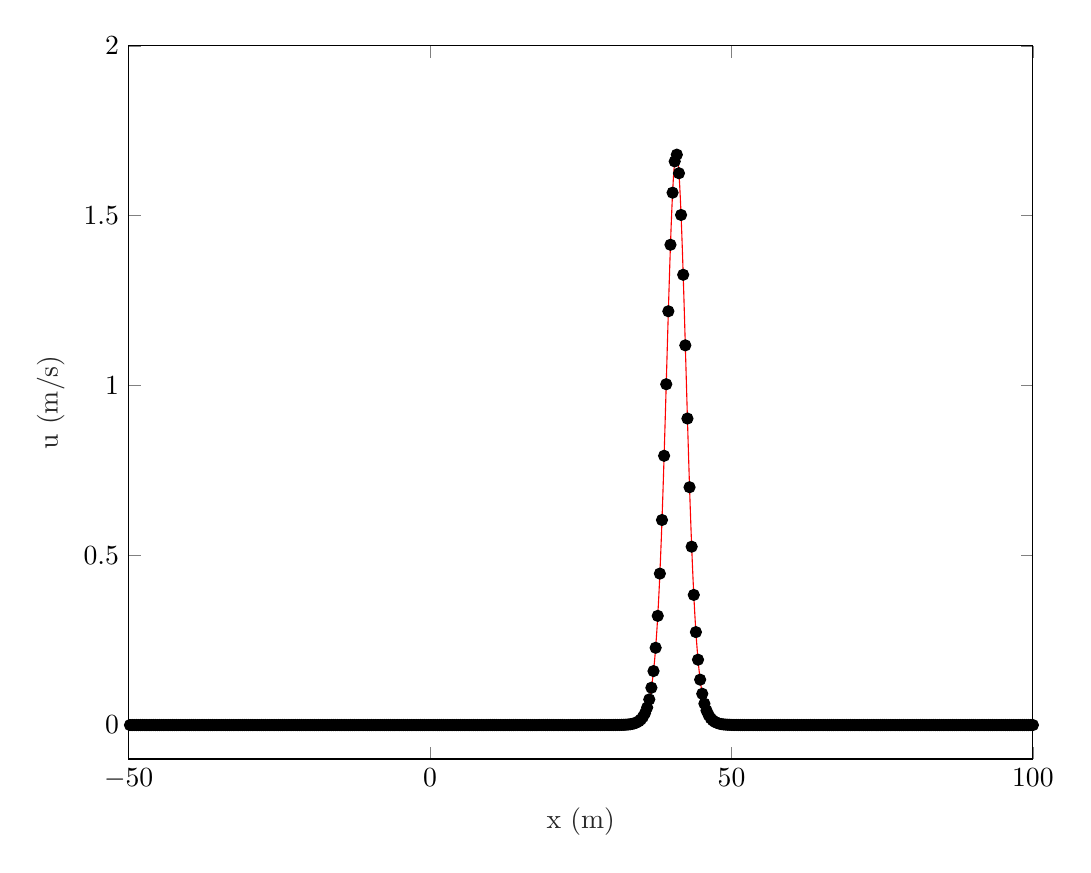
\begin{tikzpicture}

\begin{axis}[%
width=4.521in,
height=3.566in,
at={(0.758in,0.481in)},
scale only axis,
xmin=-50,
xmax=100,
xtick={-50,   0,  50, 100},
xlabel style={font=\color{white!15!black}},
xlabel={x (m)},
ymin=-0.1,
ymax=2,
ytick={  0, 0.5,   1, 1.5,   2},
ylabel style={font=\color{white!15!black}},
ylabel={u (m/s)},
axis background/.style={fill=white}
]
\addplot [color=red, forget plot]
  table[row sep=crcr]{%
-50.14064697609	0\\
-50.0234411626817	0\\
-49.9062353492733	0\\
-49.789029535865	0\\
-49.6718237224566	0\\
-49.5546179090483	0\\
-49.4374120956399	0\\
-49.3202062822316	0\\
-49.2030004688233	0\\
-49.0857946554149	0\\
-48.9685888420066	0\\
-48.8513830285982	0\\
-48.7341772151899	0\\
-48.6169714017815	0\\
-48.4997655883732	0\\
-48.3825597749648	0\\
-48.2653539615565	0\\
-48.1481481481481	0\\
-48.0309423347398	0\\
-47.9137365213315	0\\
-47.7965307079231	0\\
-47.6793248945148	0\\
-47.5621190811064	0\\
-47.4449132676981	0\\
-47.3277074542897	0\\
-47.2105016408814	0\\
-47.093295827473	0\\
-46.9760900140647	0\\
-46.8588842006564	0\\
-46.741678387248	0\\
-46.6244725738397	0\\
-46.5072667604313	0\\
-46.390060947023	0\\
-46.2728551336146	0\\
-46.1556493202063	0\\
-46.0384435067979	0\\
-45.9212376933896	0\\
-45.8040318799812	0\\
-45.6868260665729	0\\
-45.5696202531646	0\\
-45.4524144397562	0\\
-45.3352086263479	0\\
-45.2180028129395	0\\
-45.1007969995312	0\\
-44.9835911861228	0\\
-44.8663853727145	0\\
-44.7491795593061	0\\
-44.6319737458978	0\\
-44.5147679324894	0\\
-44.3975621190811	0\\
-44.2803563056728	0\\
-44.1631504922644	0\\
-44.0459446788561	0\\
-43.9287388654477	0\\
-43.8115330520394	0\\
-43.694327238631	0\\
-43.5771214252227	0\\
-43.4599156118143	0\\
-43.342709798406	0\\
-43.2255039849977	0\\
-43.1082981715893	0\\
-42.991092358181	0\\
-42.8738865447726	0\\
-42.7566807313643	0\\
-42.6394749179559	0\\
-42.5222691045476	0\\
-42.4050632911392	0\\
-42.2878574777309	0\\
-42.1706516643225	0\\
-42.0534458509142	0\\
-41.9362400375059	0\\
-41.8190342240975	0\\
-41.7018284106892	0\\
-41.5846225972808	0\\
-41.4674167838725	0\\
-41.3502109704641	0\\
-41.2330051570558	0\\
-41.1157993436474	0\\
-40.9985935302391	0\\
-40.8813877168308	0\\
-40.7641819034224	0\\
-40.6469760900141	0\\
-40.5297702766057	0\\
-40.4125644631974	0\\
-40.295358649789	0\\
-40.1781528363807	0\\
-40.0609470229723	0\\
-39.943741209564	0\\
-39.8265353961556	0\\
-39.7093295827473	0\\
-39.592123769339	0\\
-39.4749179559306	0\\
-39.3577121425223	0\\
-39.2405063291139	0\\
-39.1233005157056	0\\
-39.0060947022972	0\\
-38.8888888888889	0\\
-38.7716830754805	0\\
-38.6544772620722	0\\
-38.5372714486639	0\\
-38.4200656352555	0\\
-38.3028598218472	0\\
-38.1856540084388	0\\
-38.0684481950305	0\\
-37.9512423816221	0\\
-37.8340365682138	0\\
-37.7168307548054	0\\
-37.5996249413971	0\\
-37.4824191279887	0\\
-37.3652133145804	0\\
-37.2480075011721	0\\
-37.1308016877637	0\\
-37.0135958743554	0\\
-36.896390060947	0\\
-36.7791842475387	0\\
-36.6619784341303	0\\
-36.544772620722	0\\
-36.4275668073136	0\\
-36.3103609939053	0\\
-36.193155180497	0\\
-36.0759493670886	0\\
-35.9587435536803	0\\
-35.8415377402719	0\\
-35.7243319268636	0\\
-35.6071261134552	0\\
-35.4899203000469	0\\
-35.3727144866385	0\\
-35.2555086732302	0\\
-35.1383028598218	0\\
-35.0210970464135	0\\
-34.9038912330052	0\\
-34.7866854195968	0\\
-34.6694796061885	0\\
-34.5522737927801	0\\
-34.4350679793718	0\\
-34.3178621659634	0\\
-34.2006563525551	0\\
-34.0834505391467	0\\
-33.9662447257384	0\\
-33.8490389123301	0\\
-33.7318330989217	0\\
-33.6146272855134	0\\
-33.497421472105	0\\
-33.3802156586967	0\\
-33.2630098452883	0\\
-33.14580403188	0\\
-33.0285982184716	0\\
-32.9113924050633	0\\
-32.7941865916549	0\\
-32.6769807782466	0\\
-32.5597749648383	0\\
-32.4425691514299	0\\
-32.3253633380216	0\\
-32.2081575246132	0\\
-32.0909517112049	0\\
-31.9737458977965	0\\
-31.8565400843882	0\\
-31.7393342709798	0\\
-31.6221284575715	0\\
-31.5049226441632	0\\
-31.3877168307548	0\\
-31.2705110173465	0\\
-31.1533052039381	0\\
-31.0360993905298	0\\
-30.9188935771214	0\\
-30.8016877637131	0\\
-30.6844819503047	0\\
-30.5672761368964	0\\
-30.450070323488	0\\
-30.3328645100797	0\\
-30.2156586966714	0\\
-30.098452883263	0\\
-29.9812470698547	0\\
-29.8640412564463	0\\
-29.746835443038	0\\
-29.6296296296296	0\\
-29.5124238162213	0\\
-29.3952180028129	0\\
-29.2780121894046	0\\
-29.1608063759962	0\\
-29.0436005625879	0\\
-28.9263947491796	0\\
-28.8091889357712	0\\
-28.6919831223629	0\\
-28.5747773089545	0\\
-28.4575714955462	0\\
-28.3403656821378	0\\
-28.2231598687295	0\\
-28.1059540553211	0\\
-27.9887482419128	0\\
-27.8715424285045	0\\
-27.7543366150961	0\\
-27.6371308016878	0\\
-27.5199249882794	0\\
-27.4027191748711	0\\
-27.2855133614627	0\\
-27.1683075480544	0\\
-27.051101734646	0\\
-26.9338959212377	0\\
-26.8166901078293	0\\
-26.699484294421	0\\
-26.5822784810127	0\\
-26.4650726676043	0\\
-26.347866854196	0\\
-26.2306610407876	0\\
-26.1134552273793	0\\
-25.9962494139709	0\\
-25.8790436005626	0\\
-25.7618377871542	0\\
-25.6446319737459	0\\
-25.5274261603376	0\\
-25.4102203469292	0\\
-25.2930145335209	0\\
-25.1758087201125	0\\
-25.0586029067042	0\\
-24.9413970932958	0\\
-24.8241912798875	0\\
-24.7069854664791	0\\
-24.5897796530708	0\\
-24.4725738396624	0\\
-24.3553680262541	0\\
-24.2381622128458	0\\
-24.1209563994374	0\\
-24.0037505860291	0\\
-23.8865447726207	0\\
-23.7693389592124	0\\
-23.652133145804	0\\
-23.5349273323957	0\\
-23.4177215189873	0\\
-23.300515705579	0\\
-23.1833098921707	0\\
-23.0661040787623	0\\
-22.948898265354	0\\
-22.8316924519456	0\\
-22.7144866385373	0\\
-22.5972808251289	0\\
-22.4800750117206	0\\
-22.3628691983122	0\\
-22.2456633849039	0\\
-22.1284575714955	0\\
-22.0112517580872	0\\
-21.8940459446789	0\\
-21.7768401312705	0\\
-21.6596343178622	0\\
-21.5424285044538	0\\
-21.4252226910455	0\\
-21.3080168776371	0\\
-21.1908110642288	0\\
-21.0736052508204	0\\
-20.9563994374121	0\\
-20.8391936240038	0\\
-20.7219878105954	0\\
-20.6047819971871	0\\
-20.4875761837787	0\\
-20.3703703703704	0\\
-20.253164556962	0\\
-20.1359587435537	0\\
-20.0187529301453	0\\
-19.901547116737	0\\
-19.7843413033286	0\\
-19.6671354899203	0\\
-19.549929676512	0\\
-19.4327238631036	0\\
-19.3155180496953	0\\
-19.1983122362869	0\\
-19.0811064228786	0\\
-18.9639006094702	0\\
-18.8466947960619	0\\
-18.7294889826535	0\\
-18.6122831692452	0\\
-18.4950773558368	0\\
-18.3778715424285	0\\
-18.2606657290202	0\\
-18.1434599156118	0\\
-18.0262541022035	0\\
-17.9090482887951	0\\
-17.7918424753868	0\\
-17.6746366619784	0\\
-17.5574308485701	0\\
-17.4402250351617	0\\
-17.3230192217534	0\\
-17.2058134083451	0\\
-17.0886075949367	0\\
-16.9714017815284	0\\
-16.85419596812	0\\
-16.7369901547117	0\\
-16.6197843413033	0\\
-16.502578527895	0\\
-16.3853727144866	0\\
-16.2681669010783	0\\
-16.1509610876699	0\\
-16.0337552742616	0\\
-15.9165494608533	0\\
-15.7993436474449	0\\
-15.6821378340366	0\\
-15.5649320206282	0\\
-15.4477262072199	0\\
-15.3305203938115	0\\
-15.2133145804032	0\\
-15.0961087669948	0\\
-14.9789029535865	0\\
-14.8616971401782	0\\
-14.7444913267698	0\\
-14.6272855133615	0\\
-14.5100796999531	0\\
-14.3928738865448	0\\
-14.2756680731364	0\\
-14.1584622597281	0\\
-14.0412564463197	0\\
-13.9240506329114	0\\
-13.806844819503	0\\
-13.6896390060947	0\\
-13.5724331926864	0\\
-13.455227379278	0\\
-13.3380215658697	0\\
-13.2208157524613	0\\
-13.103609939053	0\\
-12.9864041256446	0\\
-12.8691983122363	0\\
-12.7519924988279	0\\
-12.6347866854196	0\\
-12.5175808720113	0\\
-12.4003750586029	0\\
-12.2831692451946	0\\
-12.1659634317862	0\\
-12.0487576183779	0\\
-11.9315518049695	0\\
-11.8143459915612	0\\
-11.6971401781528	0\\
-11.5799343647445	0\\
-11.4627285513361	0\\
-11.3455227379278	0\\
-11.2283169245195	0\\
-11.1111111111111	0\\
-10.9939052977028	0\\
-10.8766994842944	0\\
-10.7594936708861	0\\
-10.6422878574777	0\\
-10.5250820440694	0\\
-10.407876230661	0\\
-10.2906704172527	0\\
-10.1734646038444	0\\
-10.056258790436	0\\
-9.93905297702766	0\\
-9.82184716361932	0\\
-9.70464135021097	0\\
-9.58743553680262	0\\
-9.47022972339428	0\\
-9.35302390998594	0\\
-9.23581809657759	0\\
-9.11861228316924	0\\
-9.0014064697609	0\\
-8.88420065635255	0\\
-8.76699484294421	0\\
-8.64978902953587	0\\
-8.53258321612752	0\\
-8.41537740271917	0\\
-8.29817158931083	0\\
-8.18096577590249	0\\
-8.06375996249414	0\\
-7.94655414908579	0\\
-7.82934833567745	0\\
-7.7121425222691	0\\
-7.59493670886076	0\\
-7.47773089545242	0\\
-7.36052508204407	0\\
-7.24331926863572	0\\
-7.12611345522738	0\\
-7.00890764181904	0\\
-6.89170182841069	0\\
-6.77449601500234	0\\
-6.657290201594	0\\
-6.54008438818565	0\\
-6.42287857477731	0\\
-6.30567276136896	0\\
-6.18846694796062	0\\
-6.07126113455227	0\\
-5.95405532114393	0\\
-5.83684950773559	0\\
-5.71964369432724	0\\
-5.60243788091889	0\\
-5.48523206751055	0\\
-5.3680262541022	0\\
-5.25082044069386	0\\
-5.13361462728551	0\\
-5.01640881387717	0\\
-4.89920300046882	0\\
-4.78199718706048	0\\
-4.66479137365214	0\\
-4.54758556024379	0\\
-4.43037974683544	0\\
-4.31317393342709	0\\
-4.19596812001875	0\\
-4.07876230661041	0\\
-3.96155649320206	0\\
-3.84435067979372	0\\
-3.72714486638537	0\\
-3.60993905297703	0\\
-3.49273323956868	0\\
-3.37552742616034	0\\
-3.25832161275199	0\\
-3.14111579934364	0\\
-3.0239099859353	0\\
-2.90670417252696	0\\
-2.78949835911861	0\\
-2.67229254571027	0\\
-2.55508673230192	0\\
-2.43788091889358	0\\
-2.32067510548523	0\\
-2.20346929207689	0\\
-2.08626347866854	0\\
-1.96905766526019	0\\
-1.85185185185185	0\\
-1.73464603844351	0\\
-1.61744022503516	0\\
-1.50023441162681	0\\
-1.38302859821847	0\\
-1.26582278481013	0\\
-1.14861697140178	0\\
-1.03141115799344	0\\
-0.914205344585092	0\\
-0.796999531176745	0\\
-0.679793717768398	0\\
-0.562587904360058	0\\
-0.445382090951711	0\\
-0.328176277543363	0\\
-0.210970464135023	0\\
-0.0937646507266763	0\\
0.0234411626816708	0\\
0.140646976090011	0\\
0.257852789498358	0\\
0.375058602906705	0\\
0.492264416315052	0\\
0.609470229723392	0\\
0.726676043131739	0\\
0.843881856540087	0\\
0.961087669948427	0\\
1.07829348335677	0\\
1.19549929676512	0\\
1.31270511017347	0\\
1.42991092358181	0\\
1.54711673699016	0\\
1.6643225503985	0\\
1.78152836380684	0\\
1.89873417721519	0\\
2.01593999062354	0\\
2.13314580403188	0\\
2.25035161744022	0\\
2.36755743084857	0\\
2.48476324425692	0\\
2.60196905766526	0\\
2.71917487107361	0\\
2.83638068448195	0\\
2.95358649789029	0\\
3.07079231129864	0\\
3.18799812470699	0\\
3.30520393811533	0\\
3.42240975152367	0\\
3.53961556493202	0\\
3.65682137834037	0\\
3.77402719174871	0\\
3.89123300515705	0\\
4.0084388185654	0\\
4.12564463197375	0\\
4.24285044538209	0\\
4.36005625879044	0\\
4.47726207219878	0\\
4.59446788560712	0\\
4.71167369901547	0\\
4.82887951242382	0\\
4.94608532583216	0\\
5.0632911392405	0\\
5.18049695264885	0\\
5.2977027660572	0\\
5.41490857946554	0\\
5.53211439287389	0\\
5.64932020628223	0\\
5.76652601969058	0\\
5.88373183309892	0\\
6.00093764650727	0\\
6.11814345991561	0\\
6.23534927332395	0\\
6.3525550867323	0\\
6.46976090014065	0\\
6.58696671354899	0\\
6.70417252695734	0\\
6.82137834036568	0\\
6.93858415377403	9.06774273054312e-16\\
7.05578996718237	9.06774273054312e-16\\
7.17299578059072	9.06774273054312e-16\\
7.29020159399906	9.06774273054312e-16\\
7.4074074074074	9.06774273054312e-16\\
7.52461322081575	9.06774273054312e-16\\
7.6418190342241	9.06774273054312e-16\\
7.75902484763245	9.06774273054312e-16\\
7.87623066104079	1.81354854610862e-15\\
7.99343647444913	1.81354854610862e-15\\
8.11064228785748	1.81354854610862e-15\\
8.22784810126582	1.81354854610862e-15\\
8.34505391467417	2.72032281916294e-15\\
8.46225972808251	2.72032281916294e-15\\
8.57946554149086	2.72032281916294e-15\\
8.6966713548992	3.62709709221725e-15\\
8.81387716830755	3.62709709221725e-15\\
8.9310829817159	4.53387136527156e-15\\
9.04828879512424	5.44064563832587e-15\\
9.16549460853258	5.44064563832587e-15\\
9.28270042194093	6.34741991138018e-15\\
9.39990623534927	7.2541941844345e-15\\
9.51711204875762	9.06774273054312e-15\\
9.63431786216596	9.97451700359743e-15\\
9.75152367557431	1.08812912766517e-14\\
9.86872948898265	1.26948398227604e-14\\
9.985935302391	1.4508388368869e-14\\
10.1031411157993	1.63219369149776e-14\\
10.2203469292077	1.90422597341406e-14\\
10.337552742616	2.17625825533035e-14\\
10.4547585560244	2.44829053724664e-14\\
10.5719643694327	2.81100024646837e-14\\
10.6891701828411	3.17370995569009e-14\\
10.8063759962494	3.62709709221725e-14\\
10.9235818096578	4.0804842287444e-14\\
11.0407876230661	4.71522621988242e-14\\
11.1579934364744	5.34996821102044e-14\\
11.2751992498828	6.07538762946389e-14\\
11.3924050632911	6.89148447521277e-14\\
11.5096108766995	7.88893617557252e-14\\
11.6268166901078	8.97706530323769e-14\\
11.7440225035162	1.02465492855137e-13\\
11.8612283169245	1.16973881224006e-13\\
11.9784341303329	1.33295818138984e-13\\
12.0956399437412	1.5143130360007e-13\\
12.2128457571496	1.72287111880319e-13\\
12.3300515705579	1.96770017252786e-13\\
12.4472573839662	2.23973245444415e-13\\
12.5644631973746	2.54803570728262e-13\\
12.6816690107829	2.91074541650434e-13\\
12.7988748241913	3.30972609664824e-13\\
12.9160806375996	3.77218097590594e-13\\
13.033286451008	4.29811005427744e-13\\
13.1504922644163	4.89658107449328e-13\\
13.2676980778247	5.57666177928402e-13\\
13.384903891233	6.34741991138018e-13\\
13.5021097046413	7.23605869897341e-13\\
13.6193155180497	8.2425781420637e-13\\
13.736521331458	9.38511372611213e-13\\
13.8537271448664	1.06908686793103e-12\\
13.9709329582747	1.218704622985e-12\\
14.0881387716831	1.3873646377731e-12\\
14.2053445850914	1.58050755793367e-12\\
14.3225503984998	1.80085370628586e-12\\
14.4397562119081	2.05112340564885e-12\\
14.5569620253165	2.33675730166096e-12\\
14.6741678387248	2.66228926568746e-12\\
14.7913736521331	3.03225316909362e-12\\
14.9085794655415	3.45390320606387e-12\\
15.0257852789498	3.93449357078266e-12\\
15.1429910923582	4.48218523170746e-12\\
15.2601969057665	5.10604593156883e-12\\
15.3774027191749	5.81605018737036e-12\\
15.4946085325832	6.62579961320786e-12\\
15.6118143459916	7.54708227463104e-12\\
15.7290201593999	8.59712688282793e-12\\
15.8462259728083	9.79316214898657e-12\\
15.9634317862166	1.11560438813872e-11\\
16.0806375996249	1.27084414368562e-11\\
16.1978434130333	1.44766512693121e-11\\
16.3150492264416	1.64905969297657e-11\\
16.43225503985	1.87847358405931e-11\\
16.5494608532583	2.13980592955357e-11\\
16.6666666666667	2.4375906008246e-11\\
16.783872480075	2.77672417894691e-11\\
16.9010782934834	3.16301001926805e-11\\
17.0182841068917	3.60306757398131e-11\\
17.1354899203	4.10442306955304e-11\\
17.2526957337084	4.67541882929534e-11\\
17.3699015471167	5.3259386927845e-11\\
17.4871073605251	6.06695462872449e-11\\
17.6043131739334	6.91107079951074e-11\\
17.7215189873418	7.87261423865754e-11\\
17.8387248007501	8.96799756050715e-11\\
17.9559306141585	1.02157189602299e-10\\
18.0731364275668	1.16370876332425e-10\\
18.1903422409752	1.32562237752083e-10\\
18.3075480543835	1.51005119691735e-10\\
18.4247538677918	1.72015079598403e-10\\
18.5419596812002	1.95948479761398e-10\\
18.6591654946085	2.23210648280776e-10\\
18.7763713080169	2.54266760358614e-10\\
18.8935771214252	2.89643651847554e-10\\
19.0107829348336	3.29942514090634e-10\\
19.1279887482419	3.75847961664009e-10\\
19.2451945616503	4.28140727216778e-10\\
19.3624003750586	4.87708542762262e-10\\
19.4796061884669	5.55565181937735e-10\\
19.5968120018753	6.32862248069977e-10\\
19.7140178152836	7.20913657080643e-10\\
19.831223628692	8.21216493294545e-10\\
19.9484294421003	9.35474585570754e-10\\
20.0656352555087	1.06562933762788e-09\\
20.182841068917	1.2138923719179e-09\\
20.3000468823254	1.3827845209199e-09\\
20.4172526957337	1.57517481843383e-09\\
20.5344585091421	1.79433218571406e-09\\
20.6516643225504	2.04398255824855e-09\\
20.7688701359587	2.32836691931239e-09\\
20.8860759493671	2.65231837578095e-09\\
21.0032817627754	3.02134195426596e-09\\
21.1204875761838	3.44170890563984e-09\\
21.2376933895921	3.92056189085145e-09\\
21.3548992030005	4.46603920900146e-09\\
21.4721050164088	5.08741081348329e-09\\
21.5893108298172	5.79523427715812e-09\\
21.7065166432255	6.60153977430656e-09\\
21.8237224566338	7.52002866419446e-09\\
21.9409282700422	8.56630834560963e-09\\
22.0581340834505	9.7581597552724e-09\\
22.1753398968589	1.11158366033457e-08\\
22.2925457102672	1.26624108544331e-08\\
22.4097515236756	1.44241635472906e-08\\
22.5269573370839	1.64310327413173e-08\\
22.6441631504923	1.87171222169228e-08\\
22.7613689639006	2.13212818110619e-08\\
22.878574777309	2.42877648285823e-08\\
22.9957805907173	2.76669815716461e-08\\
23.1129864041256	3.151635578803e-08\\
23.230192217534	3.5901304894115e-08\\
23.3473980309423	4.0896341705628e-08\\
23.4646038443507	4.65863502690438e-08\\
23.581809657759	5.30680240055825e-08\\
23.6990154711674	6.04515087861918e-08\\
23.8162212845757	6.88622758738088e-08\\
23.9334270979841	7.84432546564492e-08\\
24.0506329113924	8.93572573616143e-08\\
24.1678387248007	1.01789751972017e-07\\
24.2850445382091	1.15952011452635e-07\\
24.4022503516174	1.32084700042954e-07\\
24.5194561650258	1.50461968249595e-07\\
24.6366619784341	1.71396111852519e-07\\
24.7538677918425	1.95242872907434e-07\\
24.8710736052508	2.2240749337084e-07\\
24.9882794186592	2.53351593436275e-07\\
25.1054852320675	2.88601021479201e-07\\
25.2226910454759	3.2875478759714e-07\\
25.3398968588842	3.74495244871209e-07\\
25.4571026722925	4.26599682475207e-07\\
25.5743084857009	4.85953536469996e-07\\
25.6915142991092	5.53565434548849e-07\\
25.8087201125176	6.30584339058476e-07\\
25.9259259259259	7.18319067128794e-07\\
26.0431317393343	8.18260536112787e-07\\
26.1603375527426	9.32107098406299e-07\\
26.277543366151	1.06179340089945e-06\\
26.3947491795593	1.20952326053126e-06\\
26.5119549929676	1.37780711769429e-06\\
26.629160806376	1.56950469452345e-06\\
26.7463666197843	1.78787358983615e-06\\
26.8635724331927	2.03662463996857e-06\\
26.980778246601	2.31998497313827e-06\\
27.0979840600094	2.64276984682245e-06\\
27.2151898734177	3.01046446917432e-06\\
27.3323956868261	3.42931721405818e-06\\
27.4496015002344	3.90644579388892e-06\\
27.5668073136428	4.44995821787938e-06\\
27.6840131270511	5.06909056369633e-06\\
27.8012189404594	5.77436392739224e-06\\
27.9184247538678	6.57776320528796e-06\\
28.0356305672761	7.49294074640665e-06\\
28.1528363806845	8.53544833888351e-06\\
28.2700421940928	9.72300147209892e-06\\
28.3872480075012	1.10757803598941e-05\\
28.5044538209095	1.26167728395292e-05\\
28.6216596343179	1.43721649746762e-05\\
28.7388654477262	1.63717859945929e-05\\
28.8560712611346	1.86496151297085e-05\\
28.9732770745429	2.12443589439223e-05\\
29.0904828879512	2.42001089776323e-05\\
29.2076887013596	2.7567090867513e-05\\
29.3248945147679	3.14025176564703e-05\\
29.4421003281763	3.57715617881077e-05\\
29.5593061415846	4.07484622794739e-05\\
29.676511954993	4.64177858754163e-05\\
29.7937177684013	5.28758635689993e-05\\
29.9109235818097	6.02324268779463e-05\\
30.028129395218	6.8612471626214e-05\\
30.1453352086263	7.81583808349547e-05\\
30.2625410220347	8.90323427240722e-05\\
30.379746835443	0.000101419104795608\\
30.4969526488514	0.00011552911067516\\
30.6141584622597	0.000131602072815669\\
30.7313642756681	0.000149911041553117\\
30.8485700890764	0.00017076703935599\\
30.9657759024848	0.000194524338611991\\
31.0829817158931	0.000221586472133703\\
31.2001875293015	0.000252413077847617\\
31.3173933427098	0.000287527693114307\\
31.4345991561181	0.000327526630003336\\
31.5518049695265	0.000373089080882208\\
31.6690107829348	0.000424988624155939\\
31.7862165963432	0.000484106323209475\\
31.9034224097515	0.000551445637959232\\
32.0206282231599	0.000628149398278317\\
32.1378340365682	0.000715519122346805\\
32.2550398499766	0.000815037001262058\\
32.3722456633849	0.000928390914450008\\
32.4894514767932	0.00105750288927762\\
32.6066572902016	0.00120456147328252\\
32.7238631036099	0.00137205854946016\\
32.8410689170183	0.00156283119467619\\
32.9582747304266	0.00178010925943831\\
33.075480543835	0.00202756943468269\\
33.1926863572433	0.00230939666879157\\
33.3098921706517	0.00263035390653889\\
33.42709798406	0.002995861241836\\
33.5443037974684	0.00341208570866381\\
33.6615096108767	0.00388604307979318\\
33.778715424285	0.00442571320104597\\
33.8959212376934	0.00504017055957566\\
34.0131270511017	0.00573973196690971\\
34.1303328645101	0.00653612342967975\\
34.2475386779184	0.00744266847969811\\
34.3647444913268	0.00847450043594509\\
34.4819503047351	0.00964880126703259\\
34.5991561181435	0.0109850699041282\\
34.7163619315518	0.0125054230078522\\
34.8335677449601	0.0142349312998318\\
34.9507735583685	0.0162019946063359\\
35.0679793717768	0.0184387586954479\\
35.1851851851852	0.0209815767790725\\
35.3023909985935	0.0238715181430804\\
35.4195968120019	0.0271549256952327\\
35.5368026254102	0.0308840231960466\\
35.6540084388186	0.0351175714574539\\
35.7712142522269	0.0399215707299474\\
35.8884200656353	0.0453700036984107\\
36.0056258790436	0.0515456097915298\\
36.122831692452	0.0585406766774211\\
36.2400375058603	0.066457828647872\\
36.3572433192686	0.0754107838569794\\
36.474449132677	0.0855250428609074\\
36.5916549460853	0.0969384594317847\\
36.7088607594937	0.109801631109072\\
36.826066572902	0.124278031483017\\
36.9432723863104	0.140543789101873\\
37.0604781997187	0.158786999845292\\
37.177684013127	0.179206441798467\\
37.2948898265354	0.202009545932535\\
37.4120956399437	0.22740946487397\\
37.5293014533521	0.255621079244283\\
37.6465072667604	0.28685579086935\\
37.7637130801688	0.321314979698232\\
37.8809188935771	0.359182051898698\\
37.9981247069855	0.400613085141572\\
38.1153305203938	0.445726186646318\\
38.2325363338022	0.494589819921988\\
38.3497421472105	0.547210521986804\\
38.4669479606189	0.603520612124091\\
38.5841537740272	0.663366666180676\\
38.7013595874355	0.72649967006103\\
38.8185654008439	0.792567840764187\\
38.9357712142522	0.861113081704344\\
39.0529770276606	0.931571897213825\\
39.1701828410689	1.00328132053016\\
39.2873886544773	1.07549002388592\\
39.4045944678856	1.14737431737289\\
39.5218002812939	1.21805826602\\
39.6390060947023	1.28663673549676\\
39.7562119081106	1.35219988723851\\
39.873417721519	1.41385753620772\\
39.9906235349273	1.47076187989757\\
40.1078293483357	1.52212738904434\\
40.225035161744	1.56724706833021\\
40.3422409751524	1.60550477611835\\
40.4594467885607	1.63638375643018\\
40.5766526019691	1.65947191363387\\
40.6938584153774	1.67446460119774\\
40.8110642287858	1.68116577729349\\
40.9282700421941	1.679488304982\\
41.0454758556024	1.66945396779611\\
41.1626816690108	1.65119347281564\\
41.2798874824191	1.62494637213412\\
41.3970932958275	1.59106050313487\\
41.5142991092358	1.54999028046363\\
41.6315049226442	1.50229301432615\\
41.7487107360525	1.44862241540816\\
41.8659165494608	1.38971859296451\\
41.9831223628692	1.32639415235617\\
42.1003281762775	1.25951641763248\\
42.2175339896859	1.18998628483471\\
42.3347398030942	1.11871467683508\\
42.4519456165026	1.04659794179064\\
42.5691514299109	0.974493748905007\\
42.6863572433193	0.903199049253638\\
42.8035630567276	0.833431484522666\\
42.920768870136	0.765815277425135\\
43.0379746835443	0.7008721862066\\
43.1551804969527	0.639017626126788\\
43.272386310361	0.580561623139842\\
43.3895921237693	0.525713922101334\\
43.5067979371777	0.474592352456931\\
43.624003750586	0.427233462682169\\
43.7412095639944	0.383604455121435\\
43.8584153774027	0.343615557468145\\
43.9756211908111	0.307132123716976\\
44.0928270042194	0.273985935762325\\
44.2100328176277	0.243985352652912\\
44.3272386310361	0.216924111204356\\
44.4444444444444	0.192588710024351\\
44.5616502578528	0.170764405960209\\
44.6788560712611	0.151239918856142\\
44.7960618846695	0.133810981268217\\
44.9132676980778	0.118282889593725\\
45.0304735114862	0.104472217262382\\
45.1476793248945	0.0922078440667746\\
45.2648851383029	0.0813314424334248\\
45.3820909517112	0.0716975446069546\\
45.4992967651196	0.0631732966348332\\
45.6165025785279	0.0556379872581005\\
45.7337083919362	0.0489824233049075\\
45.8509142053446	0.0431082084757877\\
45.9681200187529	0.0379269697156838\\
46.0853258321613	0.0333595646920224\\
46.2025316455696	0.0293352951160212\\
46.319737458978	0.0257911435615636\\
46.4369432723863	0.0226710458282338\\
46.5541490857947	0.0199252065352604\\
46.671354899203	0.0175094623067961\\
46.7885607126113	0.0153846944228922\\
46.9057665260197	0.01351629099686\\
47.022972339428	0.0118736574557193\\
47.1401781528364	0.0104297732277176\\
47.2573839662447	0.00916079198268795\\
47.3745897796531	0.00804568244945439\\
47.4917955930614	0.00706590668768253\\
47.6090014064698	0.00620513267114321\\
47.7262072198781	0.00544897810760407\\
47.8434130332865	0.00478478254886827\\
47.9606188466948	0.00420140501100139\\
48.0778246601031	0.00368904451347711\\
48.1950304735115	0.00323908114488455\\
48.3122362869198	0.00284393546359155\\
48.4294421003282	0.00249694423831388\\
48.5466479137365	0.00219225072204547\\
48.6638537271449	0.00192470783064548\\
48.7810595405532	0.00168979276311278\\
48.8982653539616	0.00148353175357757\\
49.0154711673699	0.00130243378515719\\
49.1326769807782	0.00114343222330498\\
49.2498827941866	0.00100383344171454\\
49.3670886075949	0.000881271617858047\\
49.4842944210033	0.000773668968633056\\
49.6015002344116	0.000679200780229493\\
49.71870604782	0.000596264660961034\\
49.8359118612283	0.000523453512314844\\
49.9531176746367	0.000459531772598186\\
50.070323488045	0.000403414540043558\\
50.1875293014534	0.000354149228735224\\
50.3047351148617	0.000310899451916122\\
50.42194092827	0.000272930863634315\\
50.5391467416784	0.000239598721858688\\
50.6563525550867	0.000210336964605091\\
50.7735583684951	0.000184648615646573\\
50.8907641819034	0.000162097358477567\\
51.0079699953118	0.000142300136678561\\
51.1251758087201	0.00012492065592359\\
51.2423816221285	0.000109663678018346\\
51.3595874355368	9.62700105928315e-05\\
51.4767932489451	8.45121077680922e-05\\
51.5939990623535	7.41902074147901e-05\\
51.7112048757618	6.51289396111296e-05\\
51.8284106891702	5.71743489067714e-05\\
51.9456165025785	5.01912799321048e-05\\
52.0628223159869	4.40610820660213e-05\\
52.1800281293952	3.86795942493338e-05\\
52.2972339428036	3.39553757725054e-05\\
52.4144397562119	2.98081530316197e-05\\
52.5316455696203	2.61674559040006e-05\\
52.6488513830286	2.29714206021477e-05\\
52.7660571964369	2.01657386928834e-05\\
52.8832630098453	1.77027344350346e-05\\
53.0004688232536	1.55405547838175e-05\\
53.117674636662	1.36424582934657e-05\\
53.2348804500703	1.19761908607231e-05\\
53.3520862634787	1.05134376963164e-05\\
53.469292076887	9.22934221546216e-06\\
53.5864978902954	8.10208369414741e-06\\
53.7037037037037	7.11250648867616e-06\\
53.820909517112	6.24379454632367e-06\\
53.9381153305204	5.48118566353429e-06\\
54.0553211439287	4.8117206426874e-06\\
54.1725269573371	4.22402307924488e-06\\
54.2897327707454	3.70810605334463e-06\\
54.4069385841538	3.25520241656744e-06\\
54.5241443975621	2.85761582161884e-06\\
54.6413502109705	2.50858993510192e-06\\
54.7585560243788	2.20219362674614e-06\\
54.8757618377872	1.93322018280707e-06\\
54.9929676511955	1.69709882847348e-06\\
55.1101734646038	1.48981705448983e-06\\
55.2273792780122	1.30785243362502e-06\\
55.3445850914205	1.1481127608755e-06\\
55.4617909048289	1.00788350952327e-06\\
55.5789967182372	8.8478170126165e-07\\
55.6962025316456	7.76715410563015e-07\\
55.8134083450539	6.81848216860387e-07\\
55.9306141584623	5.98567998817575e-07\\
56.0478199718706	5.25459535691138e-07\\
56.165025785279	4.61280461943597e-07\\
56.2822315986873	4.04940150737552e-07\\
56.3994374120956	3.55481184910186e-07\\
56.516643225504	3.1206308400216e-07\\
56.6338490389123	2.73948025283137e-07\\
56.7510548523207	2.40488298529712e-07\\
56.868260665729	2.11115308667032e-07\\
56.9854664791374	1.8532990320762e-07\\
57.1026722925457	1.6269390161951e-07\\
57.2198781059541	1.4282263756123e-07\\
57.3370839193624	1.25378428293497e-07\\
57.4542897327707	1.10064836611609e-07\\
57.5714955461791	9.66216314474252e-08\\
57.6887013595874	8.48203655312391e-08\\
57.8059071729958	7.44604934911119e-08\\
57.9231129864041	6.53659660087041e-08\\
58.0403187998125	5.7382233837078e-08\\
58.1575246132208	5.03736272230475e-08\\
58.2747304266292	4.42210449929443e-08\\
58.3919362400375	3.88199319926007e-08\\
58.5091420534459	3.40785054368727e-08\\
58.6263478668542	2.99161916307922e-08\\
58.7435536802625	2.62622594607382e-08\\
58.8607594936709	2.3054613477879e-08\\
58.9779653070792	2.02387474806614e-08\\
59.0951711204876	1.77668073635993e-08\\
59.2123769338959	1.55967877152675e-08\\
59.3295827473043	1.36918118395297e-08\\
59.4467885607126	1.20195088016119e-08\\
59.563994374121	1.05514575754739e-08\\
59.6812001875293	9.26271370763817e-09\\
59.7984060009376	8.13137587908768e-09\\
59.915611814346	7.13821775491085e-09\\
60.0328176277543	6.26636335911186e-09\\
60.1500234411627	5.500996000069e-09\\
60.267229254571	4.82910981438386e-09\\
60.3844350679794	4.23928760718441e-09\\
60.5016408813877	3.72150498888202e-09\\
60.6188466947961	3.26696443547954e-09\\
60.7360525082044	2.86794113694481e-09\\
60.8532583216128	2.51765332848966e-09\\
60.9704641350211	2.21014985056003e-09\\
61.0876699484294	1.94020405624603e-09\\
61.2048757618378	1.70322948127456e-09\\
61.3220815752461	1.49519914109899e-09\\
61.4392873886545	1.3125766160544e-09\\
61.5564932020628	1.15225983135267e-09\\
61.6736990154712	1.01152393030327e-09\\
61.7909048288795	8.87977749148169e-10\\
61.9081106422879	7.79521198670962e-10\\
62.0253164556962	6.84310806774532e-10\\
62.1425222691045	6.00729794930024e-10\\
62.2597280825129	5.27357247851561e-10\\
62.3769338959212	4.62946350913695e-10\\
62.4941397093296	4.06402627568847e-10\\
62.6113455227379	3.56764897087581e-10\\
62.7285513361463	3.13189859395956e-10\\
62.8457571495546	2.7493758668716e-10\\
62.962962962963	2.41357015033139e-10\\
63.0801687763713	2.11877783416144e-10\\
63.1973745897797	1.85999352437447e-10\\
63.314580403188	1.63281936574617e-10\\
63.4317862165964	1.4333834321306e-10\\
63.5489920300047	1.25831252323201e-10\\
63.666197843413	1.10462335169203e-10\\
63.7834036568214	9.69704407604281e-11\\
63.9006094702297	8.51270619800658e-11\\
64.0178152836381	7.4729081390952e-11\\
64.1350210970464	6.56023983326603e-11\\
64.2522269104548	5.75892340816794e-11\\
64.3694327238631	5.05553860455971e-11\\
64.4866385372714	4.43811600203702e-11\\
64.6038443506798	3.89604634160516e-11\\
64.7210501640881	3.42017120310625e-11\\
64.8382559774965	3.00242029551013e-11\\
64.9554617909048	2.63572077948697e-11\\
65.0726676043132	2.31381591255269e-11\\
65.1898734177215	2.03117437164166e-11\\
65.3070792311299	1.783080930534e-11\\
65.4242850445382	1.56527375014635e-11\\
65.5414908579466	1.3741257333865e-11\\
65.6586966713549	1.20628181544415e-11\\
65.7759024847633	1.05893099607283e-11\\
65.8931082981716	9.29624984735281e-12\\
66.0103141115799	8.16096845748881e-12\\
66.1275199249883	7.16442353140212e-12\\
66.2447257383966	6.28938635790471e-12\\
66.361931551805	5.52044177435465e-12\\
66.4791373652133	4.8467084894753e-12\\
66.5963431786217	4.25458488917083e-12\\
66.71354899203	3.73500323071071e-12\\
66.8307548054383	3.27889577136439e-12\\
66.9479606188467	2.87810154267439e-12\\
67.065166432255	2.52717989900237e-12\\
67.1823722456634	2.21796987189085e-12\\
67.2995780590717	1.94684436424761e-12\\
67.4167838724801	1.70926950470738e-12\\
67.5339896858884	1.50071142190489e-12\\
67.6511954992968	1.31754301874792e-12\\
67.7684013127051	1.15613719814425e-12\\
67.8856071261135	1.01558718582083e-12\\
68.0028129395218	8.91359110412389e-13\\
68.1200187529302	7.82546197645871e-13\\
68.2372245663385	6.86428124702114e-13\\
68.3544303797468	6.03004891581117e-13\\
68.4716361931552	5.29556175463718e-13\\
68.5888420065635	4.64268427803808e-13\\
68.7060478199719	4.0804842287444e-13\\
68.8232536333802	3.58175837856453e-13\\
68.9404594467886	3.14650672749846e-13\\
69.0576652601969	2.75659379008511e-13\\
69.1748710736052	2.42108730905501e-13\\
69.2920768870136	2.13091954167763e-13\\
69.4092827004219	1.86795500249188e-13\\
69.5264885138303	1.6412614342283e-13\\
69.6436943272386	1.44177109415636e-13\\
69.760900140647	1.26041623954549e-13\\
69.8781059540553	1.10626461312626e-13\\
69.9953117674637	9.70248472168114e-14\\
70.112517580872	8.52367816671053e-14\\
70.2297233942804	7.52622646635079e-14\\
70.3469292076887	6.61945219329648e-14\\
70.4641350210971	5.8033553475476e-14\\
70.5813408345054	5.07793592910415e-14\\
70.6985466479137	4.44319393796613e-14\\
70.8157524613221	3.89912937413354e-14\\
70.9329582747304	3.44574223760639e-14\\
71.0501640881388	2.99235510107923e-14\\
71.1673699015471	2.6296453918575e-14\\
71.2845757149555	2.35761310994121e-14\\
71.4017815283638	1.99490340071949e-14\\
71.5189873417721	1.81354854610862e-14\\
71.6361931551805	1.54151626419233e-14\\
71.7533989685888	1.36016140958147e-14\\
71.8706047819972	1.17880655497061e-14\\
71.9878105954055	1.08812912766517e-14\\
72.1050164088139	9.06774273054312e-15\\
72.2222222222222	8.16096845748881e-15\\
72.3394280356306	7.2541941844345e-15\\
72.4566338490389	6.34741991138018e-15\\
72.5738396624473	5.44064563832587e-15\\
72.6910454758556	4.53387136527156e-15\\
72.8082512892639	4.53387136527156e-15\\
72.9254571026723	3.62709709221725e-15\\
73.0426629160806	3.62709709221725e-15\\
73.159868729489	2.72032281916294e-15\\
73.2770745428973	2.72032281916294e-15\\
73.3942803563057	1.81354854610862e-15\\
73.511486169714	1.81354854610862e-15\\
73.6286919831224	1.81354854610862e-15\\
73.7458977965307	1.81354854610862e-15\\
73.8631036099391	9.06774273054312e-16\\
73.9803094233474	9.06774273054312e-16\\
74.0975152367557	9.06774273054312e-16\\
74.2147210501641	9.06774273054312e-16\\
74.3319268635724	9.06774273054312e-16\\
74.4491326769808	9.06774273054312e-16\\
74.5663384903891	9.06774273054312e-16\\
74.6835443037975	9.06774273054312e-16\\
74.8007501172058	9.06774273054312e-16\\
74.9179559306142	0\\
75.0351617440225	0\\
75.1523675574308	0\\
75.2695733708392	0\\
75.3867791842475	0\\
75.5039849976559	0\\
75.6211908110642	0\\
75.7383966244726	0\\
75.8556024378809	0\\
75.9728082512893	0\\
76.0900140646976	0\\
76.207219878106	0\\
76.3244256915143	0\\
76.4416315049226	0\\
76.558837318331	0\\
76.6760431317393	0\\
76.7932489451477	0\\
76.910454758556	0\\
77.0276605719644	0\\
77.1448663853727	0\\
77.2620721987811	0\\
77.3792780121894	0\\
77.4964838255977	0\\
77.6136896390061	0\\
77.7308954524144	0\\
77.8481012658228	0\\
77.9653070792311	0\\
78.0825128926395	0\\
78.1997187060478	0\\
78.3169245194562	0\\
78.4341303328645	0\\
78.5513361462729	0\\
78.6685419596812	0\\
78.7857477730896	0\\
78.9029535864979	0\\
79.0201593999062	0\\
79.1373652133146	0\\
79.2545710267229	0\\
79.3717768401313	0\\
79.4889826535396	0\\
79.606188466948	0\\
79.7233942803563	0\\
79.8406000937647	0\\
79.957805907173	0\\
80.0750117205813	0\\
80.1922175339897	0\\
80.309423347398	0\\
80.4266291608064	0\\
80.5438349742147	0\\
80.6610407876231	0\\
80.7782466010314	0\\
80.8954524144397	0\\
81.0126582278481	0\\
81.1298640412564	0\\
81.2470698546648	0\\
81.3642756680731	0\\
81.4814814814815	0\\
81.5986872948898	0\\
81.7158931082982	0\\
81.8330989217065	0\\
81.9503047351149	0\\
82.0675105485232	0\\
82.1847163619315	0\\
82.3019221753399	0\\
82.4191279887482	0\\
82.5363338021566	0\\
82.6535396155649	0\\
82.7707454289733	0\\
82.8879512423816	0\\
83.00515705579	0\\
83.1223628691983	0\\
83.2395686826067	0\\
83.356774496015	0\\
83.4739803094234	0\\
83.5911861228317	0\\
83.70839193624	0\\
83.8255977496484	0\\
83.9428035630567	0\\
84.0600093764651	0\\
84.1772151898734	0\\
84.2944210032818	0\\
84.4116268166901	0\\
84.5288326300985	0\\
84.6460384435068	0\\
84.7632442569152	0\\
84.8804500703235	0\\
84.9976558837318	0\\
85.1148616971402	0\\
85.2320675105485	0\\
85.3492733239569	0\\
85.4664791373652	0\\
85.5836849507735	0\\
85.7008907641819	0\\
85.8180965775902	0\\
85.9353023909986	0\\
86.0525082044069	0\\
86.1697140178153	0\\
86.2869198312236	0\\
86.404125644632	0\\
86.5213314580403	0\\
86.6385372714487	0\\
86.755743084857	0\\
86.8729488982653	0\\
86.9901547116737	0\\
87.107360525082	0\\
87.2245663384904	0\\
87.3417721518987	0\\
87.4589779653071	0\\
87.5761837787154	0\\
87.6933895921238	0\\
87.8105954055321	0\\
87.9278012189405	0\\
88.0450070323488	0\\
88.1622128457572	0\\
88.2794186591655	0\\
88.3966244725738	0\\
88.5138302859822	0\\
88.6310360993905	0\\
88.7482419127989	0\\
88.8654477262072	0\\
88.9826535396156	0\\
89.0998593530239	0\\
89.2170651664323	0\\
89.3342709798406	0\\
89.451476793249	0\\
89.5686826066573	0\\
89.6858884200656	0\\
89.803094233474	0\\
89.9203000468823	0\\
90.0375058602907	0\\
90.154711673699	0\\
90.2719174871074	0\\
90.3891233005157	0\\
90.506329113924	0\\
90.6235349273324	0\\
90.7407407407407	0\\
90.8579465541491	0\\
90.9751523675574	0\\
91.0923581809658	0\\
91.2095639943741	0\\
91.3267698077825	0\\
91.4439756211908	0\\
91.5611814345991	0\\
91.6783872480075	0\\
91.7955930614158	0\\
91.9127988748242	0\\
92.0300046882325	0\\
92.1472105016409	0\\
92.2644163150492	0\\
92.3816221284576	0\\
92.4988279418659	0\\
92.6160337552743	0\\
92.7332395686826	0\\
92.850445382091	0\\
92.9676511954993	0\\
93.0848570089076	0\\
93.202062822316	0\\
93.3192686357243	0\\
93.4364744491327	0\\
93.553680262541	0\\
93.6708860759494	0\\
93.7880918893577	0\\
93.9052977027661	0\\
94.0225035161744	0\\
94.1397093295828	0\\
94.2569151429911	0\\
94.3741209563995	0\\
94.4913267698078	0\\
94.6085325832161	0\\
94.7257383966245	0\\
94.8429442100328	0\\
94.9601500234412	0\\
95.0773558368495	0\\
95.1945616502579	0\\
95.3117674636662	0\\
95.4289732770745	0\\
95.5461790904829	0\\
95.6633849038912	0\\
95.7805907172996	0\\
95.8977965307079	0\\
96.0150023441163	0\\
96.1322081575246	0\\
96.2494139709329	0\\
96.3666197843413	0\\
96.4838255977496	0\\
96.601031411158	0\\
96.7182372245663	0\\
96.8354430379747	0\\
96.952648851383	0\\
97.0698546647914	0\\
97.1870604781997	0\\
97.3042662916081	0\\
97.4214721050164	0\\
97.5386779184248	0\\
97.6558837318331	0\\
97.7730895452414	0\\
97.8902953586498	0\\
98.0075011720581	0\\
98.1247069854665	0\\
98.2419127988748	0\\
98.3591186122832	0\\
98.4763244256915	0\\
98.5935302390999	0\\
98.7107360525082	0\\
98.8279418659166	0\\
98.9451476793249	0\\
99.0623534927333	0\\
99.1795593061416	0\\
99.2967651195499	0\\
99.4139709329583	0\\
99.5311767463666	0\\
99.648382559775	0\\
99.7655883731833	0\\
99.8827941865917	0\\
100	0\\
100.117205813408	0\\
};
\addplot [color=black, draw=none, mark=*, mark options={solid, black}, forget plot]
  table[row sep=crcr]{%
-50.14064697609	0\\
-49.789029535865	1.33338460333001e-10\\
-49.4374120956399	2.97683161924035e-10\\
-49.0857946554149	4.84780876856103e-10\\
-48.7341772151899	7.08589649035313e-10\\
-48.3825597749648	9.85435419619768e-10\\
-48.0309423347398	1.33507012041878e-09\\
-47.6793248945148	1.78186157475441e-09\\
-47.3277074542897	2.35621823842691e-09\\
-46.9760900140647	3.09630325640272e-09\\
-46.6244725738397	4.05011367185402e-09\\
-46.2728551336146	5.27799556116659e-09\\
-45.9212376933896	6.8556905156935e-09\\
-45.5696202531646	8.87801304854708e-09\\
-45.2180028129395	1.14632561792719e-08\\
-44.8663853727145	1.47584537692207e-08\\
-44.5147679324894	1.89456095541628e-08\\
-44.1631504922644	2.42490356714833e-08\\
-43.8115330520394	3.09438949927862e-08\\
-43.4599156118143	3.93660717777273e-08\\
-43.1082981715893	4.99234511427992e-08\\
-42.7566807313643	6.31086536333555e-08\\
-42.4050632911392	7.95132005682686e-08\\
-42.0534458509142	9.98430389391673e-08\\
-41.7018284106892	1.24935202213762e-07\\
-41.3502109704641	1.55775281964175e-07\\
-40.9985935302391	1.93515178161188e-07\\
-40.6469760900141	2.39490396952283e-07\\
-40.295358649789	2.95235878761624e-07\\
-39.943741209564	3.62499070013603e-07\\
-39.592123769339	4.43248560216823e-07\\
-39.2405063291139	5.39676269621797e-07\\
-38.8888888888889	6.54190759327367e-07\\
-38.5372714486639	7.89398858378004e-07\\
-38.1856540084388	9.48072452121548e-07\\
-37.8340365682138	1.13309701325416e-06\\
-37.4824191279887	1.34739832978536e-06\\
-37.1308016877637	1.59384397112592e-06\\
-36.7791842475387	1.87511638241896e-06\\
-36.4275668073136	2.19355524509088e-06\\
-36.0759493670886	2.5509679456184e-06\\
-35.7243319268636	2.9484087558802e-06\\
-35.3727144866385	3.385929730142e-06\\
-35.0210970464135	3.86230941634693e-06\\
-34.6694796061885	4.37476929970734e-06\\
-34.3178621659634	4.91869233540498e-06\\
-33.9662447257384	5.48736290383691e-06\\
-33.6146272855134	6.07175279017139e-06\\
-33.2630098452883	6.66038287283543e-06\\
-32.9113924050633	7.23929472843268e-06\\
-32.5597749648383	7.7921694811506e-06\\
-32.2081575246132	8.30063221076705e-06\\
-31.8565400843882	8.74477803881816e-06\\
-31.5049226441632	9.10394964867292e-06\\
-31.1533052039381	9.35778440107857e-06\\
-30.8016877637131	9.48753156271414e-06\\
-30.450070323488	9.47761270555105e-06\\
-30.098452883263	9.31738941513813e-06\\
-29.746835443038	9.00300502242732e-06\\
-29.3952180028129	8.53921976175087e-06\\
-29.0436005625879	7.94103299954517e-06\\
-28.6919831223629	7.2348936186109e-06\\
-28.3403656821378	6.45925780893397e-06\\
-27.9887482419128	5.66424312787201e-06\\
-27.6371308016878	4.91013963788634e-06\\
-27.2855133614627	4.26458294370341e-06\\
-26.9338959212377	3.79827679022336e-06\\
-26.5822784810127	3.57927856404587e-06\\
-26.2306610407876	3.6660373891874e-06\\
-25.8790436005626	4.09953103192624e-06\\
-25.5274261603376	4.89521633880276e-06\\
-25.1758087201125	6.03552120980725e-06\\
-24.8241912798875	7.46400492920237e-06\\
-24.4725738396624	9.08233086174378e-06\\
-24.1209563994374	1.07512386061004e-05\\
-23.7693389592124	1.22965473827971e-05\\
-23.4177215189873	1.35208711263208e-05\\
-23.0661040787623	1.42211551585144e-05\\
-22.7144866385373	1.42113457850028e-05\\
-22.3628691983122	1.33486669822111e-05\\
-22.0112517580872	1.15606662919009e-05\\
-21.6596343178622	8.86968860553053e-06\\
-21.3080168776371	5.41037826320181e-06\\
-20.9563994374121	1.43578881469432e-06\\
-20.6047819971871	-2.69188807627503e-06\\
-20.253164556962	-6.5286387687305e-06\\
-19.901547116737	-9.59443239839944e-06\\
-19.549929676512	-1.14349347720072e-05\\
-19.1983122362869	-1.16929742521157e-05\\
-18.8466947960619	-1.01804136466077e-05\\
-18.4950773558368	-6.93745537747186e-06\\
-18.1434599156118	-2.2664873880967e-06\\
-17.7918424753868	3.27238205904421e-06\\
-17.4402250351617	8.91225734259901e-06\\
-17.0886075949367	1.37780552277431e-05\\
-16.7369901547117	1.70244119861747e-05\\
-16.3853727144866	1.79938835555958e-05\\
-16.0337552742616	1.63674358908694e-05\\
-15.6821378340366	1.22730124369411e-05\\
-15.3305203938115	6.31954067837748e-06\\
-14.9789029535865	-4.66459827786461e-07\\
-14.6272855133615	-6.8071375427286e-06\\
-14.2756680731364	-1.14228685091052e-05\\
-13.9240506329114	-1.33197074966286e-05\\
-13.5724331926864	-1.20487428815103e-05\\
-13.2208157524613	-7.86586971660065e-06\\
-12.8691983122363	-1.72889784779393e-06\\
-12.5175808720113	4.89042874755737e-06\\
-12.1659634317862	1.03570033485027e-05\\
-11.8143459915612	1.33053995705225e-05\\
-11.4627285513361	1.30348254866004e-05\\
-11.1111111111111	9.73855177098587e-06\\
-10.7594936708861	4.47093027824887e-06\\
-10.407876230661	-1.16108560149178e-06\\
-10.056258790436	-5.50247978588365e-06\\
-9.70464135021097	-7.38542093395537e-06\\
-9.35302390998594	-6.50065063271628e-06\\
-9.0014064697609	-3.45877861838807e-06\\
-8.64978902953587	4.88860884639841e-07\\
-8.29817158931083	3.95180248194184e-06\\
-7.94655414908579	5.90999997420874e-06\\
-7.59493670886076	6.01565401880961e-06\\
-7.24331926863572	4.58507948615589e-06\\
-6.89170182841069	2.34086155445585e-06\\
-6.54008438818565	8.3484099356668e-08\\
-6.18846694796062	-1.54164800891977e-06\\
-5.83684950773559	-2.13994513579281e-06\\
-5.48523206751055	-1.60542164304645e-06\\
-5.13361462728551	-1.75206193087525e-07\\
-4.78199718706048	1.55557340646471e-06\\
-4.43037974683544	2.80792776510332e-06\\
-4.07876230661041	3.01060369527548e-06\\
-3.72714486638537	2.16761931763061e-06\\
-3.37552742616034	8.6323669531977e-07\\
-3.0239099859353	-1.51322496199073e-07\\
-2.67229254571027	-4.42385460057819e-07\\
-2.32067510548523	-6.76488720261088e-08\\
-1.96905766526019	6.19124820139388e-07\\
-1.61744022503516	1.25945939480123e-06\\
-1.26582278481013	1.59859610850754e-06\\
-0.914205344585092	1.43978048622033e-06\\
-0.562587904360058	7.65155586848382e-07\\
-0.210970464135023	1.5111471142476e-07\\
0.140646976090011	5.06466123961307e-07\\
0.492264416315052	9.72559718048777e-07\\
0.843881856540087	-3.66260039581897e-07\\
1.19549929676512	2.52593316886242e-06\\
1.54711673699016	-8.97240389414172e-07\\
1.89873417721519	2.11841862850306e-06\\
2.25035161744022	2.89815507368055e-06\\
2.60196905766526	-2.92939859289772e-06\\
2.95358649789029	-1.45517892091045e-06\\
3.30520393811533	2.53665270503579e-06\\
3.65682137834037	2.86250263104739e-06\\
4.0084388185654	9.17549263987616e-07\\
4.36005625879044	3.88238121310314e-07\\
4.71167369901547	1.50438412555082e-06\\
5.0632911392405	1.65979269698056e-06\\
5.41490857946554	-6.66013063674313e-07\\
5.76652601969058	-3.8489196101008e-06\\
6.11814345991561	-4.57148815642802e-06\\
6.46976090014065	-8.5527678376652e-07\\
6.82137834036568	5.98596134761942e-06\\
7.17299578059072	1.18085001616355e-05\\
7.52461322081575	1.21128199733487e-05\\
7.87623066104079	5.00978989529216e-06\\
8.22784810126582	-7.09699600723886e-06\\
8.57946554149086	-1.82554646713343e-05\\
8.9310829817159	-2.19066691412211e-05\\
9.28270042194093	-1.44927089019543e-05\\
9.63431786216596	2.26370213678297e-06\\
9.985935302391	2.17160422376225e-05\\
10.337552742616	3.51531109605485e-05\\
10.6891701828411	3.5743194667307e-05\\
11.0407876230661	2.16723176047534e-05\\
11.3924050632911	-2.90744228276169e-06\\
11.7440225035162	-2.94435851524277e-05\\
12.0956399437412	-4.82532914900231e-05\\
12.4472573839662	-5.21040870541994e-05\\
12.7988748241913	-3.87344314533261e-05\\
13.1504922644163	-1.1522738508942e-05\\
13.5021097046413	2.17664233108984e-05\\
13.8537271448664	5.15275174257327e-05\\
14.2053445850914	6.92210581797928e-05\\
14.5569620253165	6.97283963718468e-05\\
14.9085794655415	5.25445026800695e-05\\
15.2601969057665	2.16374647334924e-05\\
15.6118143459916	-1.58264106320662e-05\\
15.9634317862166	-5.14001671304291e-05\\
16.3150492264416	-7.73663631481213e-05\\
16.6666666666667	-8.83562148743366e-05\\
17.0182841068917	-8.22726577193526e-05\\
17.3699015471167	-6.04256687277781e-05\\
17.7215189873418	-2.69755655497294e-05\\
18.0731364275668	1.20983117809022e-05\\
18.4247538677918	5.02235567137054e-05\\
18.7763713080169	8.13995328994789e-05\\
19.1279887482419	0.000101103928509701\\
19.4796061884669	0.000106830380149672\\
19.831223628692	9.82309767942453e-05\\
20.182841068917	7.69190664709327e-05\\
20.5344585091421	4.60137341586153e-05\\
20.8860759493671	9.54866986732589e-06\\
21.2376933895921	-2.8146937308462e-05\\
21.5893108298172	-6.30031691085769e-05\\
21.9409282700422	-9.16398219744765e-05\\
22.2925457102672	-0.000111641202414316\\
22.6441631504923	-0.000121672049906627\\
22.9957805907173	-0.00012145286403121\\
23.3473980309423	-0.000111625995859635\\
23.6990154711674	-9.35527147025921e-05\\
24.0506329113924	-6.90746597200956e-05\\
24.4022503516174	-4.02755350928353e-05\\
24.7538677918425	-9.26603568936536e-06\\
25.1054852320675	2.19916641545095e-05\\
25.4571026722925	5.18120442714712e-05\\
25.8087201125176	7.88661596796757e-05\\
26.1603375527426	0.00010221774593123\\
26.5119549929676	0.000121323570216104\\
26.8635724331927	0.000136007890588552\\
27.2151898734177	0.000146421567512505\\
27.5668073136428	0.000152996152810016\\
27.9184247538678	0.000156403012351134\\
28.2700421940928	0.00015752637873783\\
28.6216596343179	0.000157460003762371\\
28.9732770745429	0.000157537379828985\\
29.3248945147679	0.000159408065331927\\
29.676511954993	0.000165177390956274\\
30.028129395218	0.000177634047744857\\
30.379746835443	0.000200601630226612\\
30.7313642756681	0.00023946837018136\\
31.0829817158931	0.000301975172560501\\
31.4345991561181	0.000399381401682303\\
31.7862165963432	0.000548185394763086\\
32.1378340365682	0.000772661124021514\\
32.4894514767932	0.00110859609368907\\
32.8410689170183	0.00160879573018789\\
33.1926863572433	0.00235118032036556\\
33.5443037974684	0.00345067420976741\\
33.8959212376934	0.00507661379726201\\
34.2475386779184	0.00747812467473998\\
34.5991561181435	0.0110208703437883\\
34.9507735583685	0.0162397313646728\\
35.3023909985935	0.023913155322768\\
35.6540084388186	0.0351655747242331\\
36.0056258790436	0.0516030757412987\\
36.3572433192686	0.0754815250080598\\
36.7088607594937	0.109890130259016\\
37.0604781997187	0.158898096918303\\
37.4120956399437	0.227547624153226\\
37.7637130801688	0.321483118047236\\
38.1153305203938	0.445924474351723\\
38.4669479606189	0.603746298023641\\
38.8185654008439	0.792817118673329\\
39.1701828410689	1.00355209353713\\
39.5218002812939	1.21834919771698\\
39.873417721519	1.41415945831959\\
40.225035161744	1.56753071553904\\
40.5766526019691	1.6596828370047\\
40.9282700421941	1.67955967215572\\
41.2798874824191	1.6248071278677\\
41.6315049226442	1.50192145874534\\
41.9831223628692	1.32582511212789\\
42.3347398030942	1.11803175882983\\
42.6863572433193	0.902502532105264\\
43.0379746835443	0.70024305133121\\
43.3895921237693	0.5251954251378\\
43.7412095639944	0.383205054295822\\
44.0928270042194	0.273692789085065\\
44.4444444444444	0.192380685949561\\
44.7960618846695	0.133666743006399\\
45.1476793248945	0.0921094004933563\\
45.4992967651196	0.0631068275769737\\
45.8509142053446	0.0430636583783803\\
46.2025316455696	0.0293055881411815\\
46.5541490857947	0.0199054685396702\\
46.9057665260197	0.0135032107593485\\
47.2573839662447	0.00915214068746264\\
47.6090014064698	0.00619941939575142\\
47.9606188466948	0.00419763670175195\\
48.3122362869198	0.00284145267892262\\
48.6638537271449	0.0019230736278294\\
49.0154711673699	0.0013013591288934\\
49.3670886075949	0.000880565564113807\\
49.71870604782	0.000595801205402249\\
50.070323488045	0.000403110612087593\\
50.42194092827	0.000272731745985402\\
50.7735583684951	0.00018451829744477\\
51.1251758087201	0.000124835457366575\\
51.4767932489451	8.44564708499167e-05\\
51.8284106891702	5.71380606865588e-05\\
52.1800281293952	3.86559566021621e-05\\
52.5316455696203	2.61520800695171e-05\\
52.8832630098453	1.76927476828345e-05\\
53.2348804500703	1.1969714801676e-05\\
53.5864978902954	8.09789149363538e-06\\
53.9381153305204	5.47847700698863e-06\\
54.2897327707454	3.70635952694811e-06\\
54.6413502109705	2.50746630778487e-06\\
54.9929676511955	1.69637771945165e-06\\
55.3445850914205	1.14765123033039e-06\\
55.6962025316456	7.76420904722807e-07\\
56.0478199718706	5.25272239266963e-07\\
56.3994374120956	3.55362517696208e-07\\
56.7510548523207	2.40413432374381e-07\\
57.1026722925457	1.62646898212157e-07\\
57.4542897327707	1.10035492490217e-07\\
57.8059071729958	7.44422919045005e-08\\
58.1575246132208	5.03624240407031e-08\\
58.5091420534459	3.40716738487044e-08\\
58.8607594936709	2.30504960266635e-08\\
59.2123769338959	1.55943412587129e-08\\
59.563994374121	1.05500298972171e-08\\
59.915611814346	7.13740328482286e-09\\
60.267229254571	4.82865955342946e-09\\
60.6188466947961	3.26672901355118e-09\\
60.9704641350211	2.21003698529753e-09\\
61.3220815752461	1.49515312322148e-09\\
61.6736990154712	1.01151299941455e-09\\
62.0253164556962	6.84316859708497e-10\\
62.3769338959212	4.62959653876683e-10\\
62.7285513361463	3.1320468677996e-10\\
63.0801687763713	2.1189060375864e-10\\
63.4317862165964	1.4334776924921e-10\\
63.7834036568214	9.69746749057455e-11\\
64.1350210970464	6.56014378382334e-11\\
64.4866385372714	4.43758147236879e-11\\
64.8382559774965	3.00151205186676e-11\\
65.1898734177215	2.02989530847071e-11\\
65.5414908579466	1.37252951033395e-11\\
65.8931082981716	9.27785881117845e-12\\
66.2447257383966	6.26868289800291e-12\\
66.5963431786217	4.23293285990774e-12\\
66.9479606188467	2.8559661972924e-12\\
67.2995780590717	1.92436607486338e-12\\
67.6511954992968	1.29359752940449e-12\\
68.0028129395218	8.66425773849346e-13\\
68.3544303797468	5.7703314610401e-13\\
68.7060478199719	3.81084563217604e-13\\
69.0576652601969	2.48790289699558e-13\\
69.4092827004219	1.59803308822346e-13\\
69.760900140647	1.00241397692199e-13\\
70.112517580872	6.05766916283951e-14\\
70.4641350210971	3.47860386229237e-14\\
70.8157524613221	1.90326435651417e-14\\
71.1673699015471	1.03519834535999e-14\\
71.5189873417721	5.63051375689482e-15\\
71.8706047819972	3.06247448217831e-15\\
72.2222222222222	1.66570056640189e-15\\
72.5738396624473	9.05985794512825e-16\\
72.9254571026723	4.92771796093029e-16\\
73.2770745428973	2.68021909941009e-16\\
73.6286919831224	1.45778928051444e-16\\
73.9803094233474	7.92901441098806e-17\\
74.3319268635724	4.31264452071361e-17\\
74.6835443037975	2.34567649874197e-17\\
75.0351617440225	1.27582929924397e-17\\
75.3867791842475	6.93932177639307e-18\\
75.7383966244726	3.77434400862703e-18\\
76.0900140646976	2.05289121249878e-18\\
76.4416315049226	1.11658140347619e-18\\
76.7932489451477	6.0731617096812e-19\\
77.1448663853727	3.30323369501866e-19\\
77.4964838255977	1.79665112926483e-19\\
77.8481012658228	9.77210690589769e-20\\
78.1997187060478	5.31511498391837e-20\\
78.5513361462729	2.89092695815922e-20\\
78.9029535864979	1.57239470880656e-20\\
79.2545710267229	8.55236108025773e-21\\
79.606188466948	4.65168698657235e-21\\
79.957805907173	2.53008398709874e-21\\
80.309423347398	1.37612977834744e-21\\
80.6610407876231	7.48486286032788e-22\\
81.0126582278481	4.07106749082871e-22\\
81.3642756680731	2.21428111966186e-22\\
81.7158931082982	1.20436246462054e-22\\
82.0675105485232	6.55060883330095e-23\\
82.4191279887482	3.56292041204061e-23\\
82.7707454289733	1.93789648956015e-23\\
83.1223628691983	1.05403499656022e-23\\
83.4739803094234	5.73296757571331e-24\\
83.8255977496484	3.1181998065946e-24\\
84.1772151898734	1.69600994693169e-24\\
84.5288326300985	9.2247127140727e-25\\
84.8804500703235	5.01738358381231e-25\\
85.2320675105485	2.72898883763665e-25\\
85.5836849507735	1.48431547071129e-25\\
85.9353023909986	8.0732921520517e-26\\
86.2869198312236	4.39111815907612e-26\\
86.6385372714487	2.38835884095534e-26\\
86.9901547116737	1.29904451361193e-26\\
87.3417721518987	7.06559089617475e-27\\
87.6933895921238	3.84302263617589e-27\\
88.0450070323488	2.09024598213803e-27\\
88.3966244725738	1.13689891511849e-27\\
88.7482419127989	6.18367002851748e-28\\
89.0998593530239	3.36333991642521e-28\\
89.451476793249	1.82934330927279e-28\\
89.803094233474	9.94992188222834e-29\\
90.154711673699	5.41182975118004e-29\\
90.506329113924	2.94353077365047e-29\\
90.8579465541491	1.60100627953752e-29\\
91.2095639943741	8.7079813469716e-30\\
91.5611814345991	4.73632990128575e-30\\
91.9127988748242	2.57612184040886e-30\\
92.2644163150492	1.40117007787463e-30\\
92.6160337552743	7.62105874158736e-31\\
92.9676511954993	4.1451453509573e-31\\
93.3192686357243	2.25457256825763e-31\\
93.6708860759494	1.22627725555291e-31\\
94.0225035161744	6.66980485772742e-32\\
94.3741209563995	3.6277519271208e-32\\
94.7257383966245	1.97315877382556e-32\\
95.0773558368495	1.07321436386508e-32\\
95.4289732770745	5.83728494678491e-33\\
95.7805907172996	3.17493780341325e-33\\
96.1322081575246	1.726868423846e-33\\
96.4838255977496	9.39252274524075e-34\\
96.8354430379747	5.10859902855756e-34\\
97.1870604781997	2.77849569786806e-34\\
97.5386779184248	1.51104800065923e-34\\
97.8902953586498	8.21511462928677e-35\\
98.2419127988748	4.46167883898779e-35\\
98.5935302390999	2.41464416230967e-35\\
98.9451476793249	1.29110748632998e-35\\
99.2967651195499	6.61364140615643e-36\\
99.648382559775	2.84564260081771e-36\\
100	1.6598024421102e-37\\
};
\end{axis}
\end{tikzpicture}%
		\caption{$t = 10s$}
	\end{subfigure}
	\begin{subfigure}{0.49\textwidth}
		\centering
		% This file was created by matlab2tikz.
%
%The latest updates can be retrieved from
%  http://www.mathworks.com/matlabcentral/fileexchange/22022-matlab2tikz-matlab2tikz
%where you can also make suggestions and rate matlab2tikz.
%
\begin{tikzpicture}

\begin{axis}[%
width=4.521in,
height=3.566in,
at={(0.758in,0.481in)},
scale only axis,
xmin=-50,
xmax=100,
xtick={-50,   0,  50, 100},
xlabel style={font=\color{white!15!black}},
xlabel={x (m)},
ymin=-0.1,
ymax=0.4,
ytick={-0.1,    0,  0.1,  0.2,  0.3,  0.4},
ylabel style={font=\color{white!15!black}},
ylabel={$\text{G (m}^\text{2}\text{/s)}$},
axis background/.style={fill=white}
]
\addplot [color=green!60!black, forget plot]
  table[row sep=crcr]{%
-50.2813379180994	1.06511867902256e-28\\
-50.0468896530166	1.91770795785705e-28\\
-49.8124413879337	3.44328815498068e-28\\
-49.5779931228509	6.16553397781048e-28\\
-49.3435448577681	1.10096737841321e-27\\
-49.1090965926852	1.96058030376556e-27\\
-48.8746483276024	3.48177937527298e-27\\
-48.6402000625195	6.16629488984274e-27\\
-48.4057517974367	1.08906489837559e-26\\
-48.1713035323539	1.91818133035259e-26\\
-47.936855267271	3.36924030658023e-26\\
-47.7024070021882	5.90174912275146e-26\\
-47.4679587371053	1.03094602732762e-25\\
-47.2335104720225	1.7959636544979e-25\\
-46.9990622069397	3.12007896947607e-25\\
-46.7646139418568	5.40555210117238e-25\\
-46.530165676774	9.33944261088278e-25\\
-46.2957174116912	1.60919356298529e-24\\
-46.0612691466083	2.76504398500092e-24\\
-45.8268208815255	4.73807826818525e-24\\
-45.5923726164426	8.09671486846486e-24\\
-45.3579243513598	1.37981826427862e-23\\
-45.123476086277	2.34499197992297e-23\\
-44.8890278211941	3.9743605460156e-23\\
-44.6545795561113	6.71737498649184e-23\\
-44.4201312910284	1.13223962895879e-22\\
-44.1856830259456	1.9031960980691e-22\\
-43.9512347608628	3.19032667155935e-22\\
-43.7167864957799	5.33326544059875e-22\\
-43.4823382306971	8.89114458826703e-22\\
-43.2478899656143	1.47818426498979e-21\\
-43.0134417005314	2.45078890661194e-21\\
-42.7789934354486	4.05218874010792e-21\\
-42.5445451703657	6.68159047799637e-21\\
-42.3100969052829	1.09869328638068e-20\\
-42.0756486402001	1.80168771168438e-20\\
-41.8412003751172	2.94638158104609e-20\\
-41.6067521100344	4.80512725964258e-20\\
-41.3723038449515	7.814968393912e-20\\
-41.1378555798687	1.26752340247965e-19\\
-40.9034073147859	2.05017614444583e-19\\
-40.668959049703	3.30698933130689e-19\\
-40.4345107846202	5.31962282227611e-19\\
-40.2000625195374	8.53365961477725e-19\\
-39.9656142544545	1.36519981313145e-18\\
-39.7311659893717	2.17802847357435e-18\\
-39.4967177242888	3.46527188191608e-18\\
-39.262269459206	5.49816165809859e-18\\
-39.0278211941232	8.69969693986612e-18\\
-38.7933729290403	1.37276807800934e-17\\
-38.5589246639575	2.16021336207052e-17\\
-38.3244763988747	3.39002228587555e-17\\
-38.0900281337918	5.30536034736352e-17\\
-37.855579868709	8.28006316232122e-17\\
-37.6211316036261	1.28872080859125e-16\\
-37.3866833385433	2.00027847259712e-16\\
-37.1522350734605	3.09619645984697e-16\\
-36.9177868083776	4.77939568538012e-16\\
-36.6833385432948	7.35739195887744e-16\\
-36.4488902782119	1.12948697787813e-15\\
-36.2144420131291	1.72919906401222e-15\\
-35.9799937480463	2.64006843150931e-15\\
-35.7455454829634	4.01968299967566e-15\\
-35.5110972178806	6.10344246265523e-15\\
-35.2766489527977	9.24196529324532e-15\\
-35.0422006877149	1.39559768513142e-14\\
-34.8077524226321	2.10166056965791e-14\\
-34.5733041575492	3.15624960322436e-14\\
-34.3388558924664	4.72701014268869e-14\\
-34.1044076273836	7.06005616758623e-14\\
-33.8699593623007	1.05156520378949e-13\\
-33.6355110972179	1.56196279969865e-13\\
-33.401062832135	2.31372422909919e-13\\
-33.1666145670522	3.417896688814e-13\\
-32.9321663019694	5.03515329246521e-13\\
-32.6977180368865	7.39729419561772e-13\\
-32.4632697718037	1.08377596215715e-12\\
-32.2288215067208	1.58347994003909e-12\\
-31.994373241638	2.30723614340874e-12\\
-31.7599249765552	3.35257078046572e-12\\
-31.5254767114723	4.85814299190808e-12\\
-31.2910284463895	7.02051642947149e-12\\
-31.0565801813067	1.01175242808807e-11\\
-30.8221319162238	1.45407189185515e-11\\
-30.587683651141	2.08402983509207e-11\\
-30.3532353860581	2.97871130373142e-11\\
-30.1187871209753	4.24579795618744e-11\\
-29.8843388558925	6.03526942479265e-11\\
-29.6498905908096	8.55540218077207e-11\\
-29.4154423257268	1.2094575401503e-10\\
-29.180994060644	1.7050897803247e-10\\
-28.9465457955611	2.39723331807462e-10\\
-28.7120975304783	3.36108725900848e-10\\
-28.4776492653954	4.69954376882962e-10\\
-28.2432010003126	6.55296787042945e-10\\
-28.0087527352298	9.11227477548806e-10\\
-27.7743044701469	1.26363604175235e-09\\
-27.5398562050641	1.74752593764382e-09\\
-27.3054079399812	2.41008125668432e-09\\
-27.0709596748984	3.31471480950272e-09\\
-26.8365114098156	4.54639411419196e-09\\
-26.6020631447327	6.21862576172907e-09\\
-26.3676148796499	8.48258443442674e-09\\
-26.1331666145671	1.1539005743999e-08\\
-25.8987183494842	1.56536282781124e-08\\
-25.6642700844014	2.11771772821244e-08\\
-25.4298218193185	2.85711391749092e-08\\
-25.1953735542357	3.8440893166905e-08\\
-24.9609252891529	5.15781560428291e-08\\
-24.72647702407	6.90151732139514e-08\\
-24.4920287589872	9.20936702842483e-08\\
-24.2575804939043	1.22552284008935e-07\\
-24.0231322288215	1.626370418028e-07\\
-23.7886839637387	2.15240479949859e-07\\
-23.5542356986558	2.84076210480409e-07\\
-23.319787433573	3.73897196493984e-07\\
-23.0853391684902	4.90767709699854e-07\\
-22.8508909034073	6.42400959105423e-07\\
-22.6164426383245	8.38576735519463e-07\\
-22.3819943732416	1.09165615410235e-06\\
-22.1475461081588	1.41721373883373e-06\\
-21.913097843076	1.83481072056946e-06\\
-21.6786495779931	2.36893755475568e-06\\
-21.4442013129103	3.05015834273556e-06\\
-21.2097530478274	3.91649509289309e-06\\
-20.9753047827446	5.01509560686489e-06\\
-20.7408565176618	6.40423523187307e-06\\
-20.5064082525789	8.1557097770862e-06\\
-20.2719599874961	1.03576845236429e-05\\
-20.0375117224133	1.31180724131416e-05\\
-19.8030634573304	1.65685230959481e-05\\
-19.5686151922476	2.08691134402079e-05\\
-19.3341669271647	2.62138391842672e-05\\
-19.0997186620819	3.28370164503466e-05\\
-18.8652703969991	4.10207105626699e-05\\
-18.6308221319162	5.11033177062736e-05\\
-18.3963738668334	6.34894320367599e-05\\
-18.1619256017505	7.86611364522268e-05\\
-17.9274773366677	9.71908588431144e-05\\
-17.6930290715849	0.000119755936651449\\
-17.458580806502	0.000147155030339543\\
-17.2241325414192	0.000180326520171261\\
-16.9896842763364	0.000220369009777762\\
-16.7552360112535	0.000268564043509115\\
-16.5207877461707	0.00032640112174009\\
-16.2863394810878	0.000395605068285114\\
-16.051891216005	0.000478165766099682\\
-15.8174429509222	0.000576370230787236\\
-15.5829946858393	0.000692836935481122\\
-15.3485464207565	0.000830552234970142\\
-15.1140981556737	0.000992908661219005\\
-14.8796498905908	0.00118374477668396\\
-14.645201625508	0.00140738617631959\\
-14.4107533604251	0.00166868712454466\\
-14.1763050953423	0.00197307220071091\\
-13.9418568302595	0.0023265772072708\\
-13.7074085651766	0.00273588847081727\\
-13.4729603000938	0.00320837953993157\\
-13.2385120350109	0.00375214415830124\\
-13.0040637699281	0.0043760242703593\\
-12.7696155048453	0.00508963170374565\\
-12.5351672397624	0.00590336207265549\\
-12.3007189746796	0.00682839936346121\\
-12.0662707095968	0.00787670960401927\\
-11.8318224445139	0.00906102198612364\\
-11.5973741794311	0.0103947958120107\\
-11.3629259143482	0.0118921716758896\\
-11.1284776492654	0.0135679053750854\\
-10.8940293841826	0.0154372831769288\\
-10.6595811190997	0.0175160172506475\\
-10.4251328540169	0.019820120310873\\
-10.190684588934	0.0223657588124346\\
-9.95623632385121	0.0251690843849017\\
-9.72178805876837	0.0282460435982727\\
-9.48733979368553	0.0316121666049176\\
-9.25289152860269	0.035282335702058\\
-9.01844326351986	0.0392705353964222\\
-8.78399499843702	0.0435895861189137\\
-8.54954673335418	0.0482508643208973\\
-8.31509846827134	0.0532640122718845\\
-8.0806502031885	0.0586366414562031\\
-7.84620193810566	0.0643740340174973\\
-7.61175367302283	0.0704788472074566\\
-7.37730540793999	0.0769508262412713\\
-7.14285714285715	0.0837865313291365\\
-6.90840887777431	0.0909790849233559\\
-6.67396061269147	0.0985179453779518\\
-6.43951234760863	0.10638871324763\\
-6.20506408252579	0.114572976343204\\
-5.97061581744295	0.123048199401807\\
-5.73616755236011	0.131787663816499\\
-5.50171928727728	0.140760462299228\\
-5.26727102219444	0.14993155262587\\
-5.0328227571116	0.159261873739066\\
-4.79837449202876	0.168708526475498\\
-4.56392622694592	0.178225020055195\\
-4.32947796186308	0.187761584242382\\
-4.09502969678024	0.197265545784949\\
-3.86058143169741	0.206681766391564\\
-3.62613316661457	0.215953138143186\\
-3.39168490153173	0.225021130892903\\
-3.15723663644889	0.233826384919695\\
-2.92278837136605	0.242309340902933\\
-2.68834010628321	0.250410898209554\\
-2.45389184120038	0.258073091567414\\
-2.21944357611754	0.265239775465496\\
-1.9849953110347	0.271857305100072\\
-1.75054704595186	0.277875202395768\\
-1.51609878086902	0.283246795586593\\
-1.28165051578619	0.287929821052489\\
-1.04720225070335	0.291886976573401\\
-0.81275398562051	0.295086415879565\\
-0.578305720537671	0.297502175331033\\
-0.343857455454831	0.29911452473196\\
-0.109409190371991	0.299910235650043\\
0.125039074710841	0.299882762137297\\
0.359487339793681	0.299032330398828\\
0.593935604876521	0.297365935691552\\
0.82838386995936	0.294897246512312\\
1.0628321350422	0.291646417910959\\
1.29728040012503	0.287639817494835\\
1.53172866520787	0.28290966933452\\
1.76617693029071	0.27749362249681\\
2.00062519537355	0.271434252283877\\
2.23507346045639	0.264778503416243\\
2.46952172553923	0.257577085336237\\
2.70396999062206	0.2498838305089\\
2.9384182557049	0.241755027046805\\
3.17286652078774	0.233248737178671\\
3.40731478587058	0.224424113020996\\
3.64176305095342	0.215340720805858\\
3.87621131603625	0.20605788418165\\
4.11065958111909	0.196634056457507\\
4.34510784620193	0.187126230732333\\
4.57955611128477	0.177589395765181\\
4.81400437636761	0.168076044237914\\
5.04845264145045	0.158635738767981\\
5.28290090653329	0.149314739683979\\
5.51734917161613	0.140155697214287\\
5.75179743669896	0.131197409393121\\
5.9862457017818	0.122474645690017\\
6.22069396686464	0.114018035146541\\
6.45514223194748	0.105854016682381\\
6.68959049703032	0.0980048482325151\\
6.92403876211316	0.0904886705136764\\
7.158487027196	0.0833196205032682\\
7.39293529227884	0.0765079891536425\\
7.62738355736168	0.0700604174613958\\
7.86183182244451	0.0639801247627084\\
8.09628008752735	0.0582671630256506\\
8.33072835261019	0.0529186909492259\\
8.56517661769303	0.047929261844275\\
8.79962488277587	0.0432911195485563\\
9.0340731478587	0.0389944970009757\\
9.26852141294154	0.035027912550687\\
9.50296967802438	0.031378459587806\\
9.73741794310722	0.0280320856360284\\
9.97186620819006	0.0249738576264334\\
10.2063144732729	0.0221882106600784\\
10.4407627383557	0.0196591781499731\\
10.6752110034386	0.0173706017976318\\
10.9096592685214	0.0153063203944778\\
11.1441075336042	0.0134503369347227\\
11.3785557986871	0.0117869639768128\\
11.6130040637699	0.0103009475899456\\
11.8474523288528	0.00897757056726193\\
12.0819005939356	0.00780273587665041\\
12.3163488590184	0.00676303155377851\\
12.5507971241013	0.00584577842155674\\
12.7852453891841	0.00503906214846849\\
13.019693654267	0.00433175123876547\\
13.2541419193498	0.00371350258486558\\
13.4885901844326	0.0031747562113406\\
13.7230384495155	0.00270672080589719\\
13.9574867145983	0.00230135157110054\\
14.1919349796812	0.0019513218465843\\
14.426383244764	0.00164998985026005\\
14.6608315098468	0.00139136177340446\\
14.8952797749297	0.00117005234288847\\
15.1297280400125	0.000981243838184623\\
15.3641763050953	0.000820644424612343\\
15.5986245701782	0.000684446540499107\\
15.833072835261	0.000569285956973589\\
16.0675211003439	0.000472202016882443\\
16.3019693654267	0.0003905994552747\\
16.5364176305095	0.000322212109028659\\
16.7708658955924	0.000265068738108604\\
17.0053141606752	0.000217461105892861\\
17.239762425758	0.000177914400974461\\
17.4742106908409	0.000145160027521762\\
17.7086589559237	0.000118110745227334\\
17.9431072210066	9.58381024498248e-05\\
18.1775554860894	7.75520766438142e-05\\
18.4120037511722	6.25828137894775e-05\\
18.6464520162551	5.03643424580478e-05\\
18.8809002813379	4.04201275583329e-05\\
19.1153485464207	3.23503229003118e-05\\
19.3497968115036	2.58205797186448e-05\\
19.5842450765864	2.05522695070437e-05\\
19.8186933416693	1.63139832697046e-05\\
20.0531416067521	1.29141750107163e-05\\
20.2875898718349	1.01948244376724e-05\\
20.5220381369178	8.02600200221367e-06\\
20.7564864020006	6.30122815557464e-06\\
20.9909346670835	4.93352774301876e-06\\
21.2253829321663	3.85208953798811e-06\\
21.4598311972491	2.99944981928463e-06\\
21.694279462332	2.32912746498166e-06\\
21.9287277274148	1.80364615921693e-06\\
22.1631759924977	1.39288690271464e-06\\
22.3976242575805	1.07272103523445e-06\\
22.6320725226633	8.23880393490863e-07\\
22.8665207877462	6.31027036827084e-07\\
23.100969052829	4.81990186134443e-07\\
23.3354173179118	3.67142662101578e-07\\
23.5698655829947	2.78893208303232e-07\\
23.8043138480775	2.11274680076135e-07\\
24.0387621131604	1.59611212178415e-07\\
24.2732103782432	1.20250189029935e-07\\
24.507658643326	9.03471730954896e-08\\
24.7421069084089	6.76939408519807e-08\\
24.9765551734917	5.05814710403796e-08\\
25.2110034385746	3.7691163351689e-08\\
25.4454517036574	2.80087713198265e-08\\
25.6798999687402	2.07565419670408e-08\\
25.9143482338231	1.53398945698486e-08\\
26.1487964989059	1.13056666569733e-08\\
26.3832447639887	8.30952897628704e-09\\
26.6176930290716	6.09064189638893e-09\\
26.8521412941544	4.45201022704086e-09\\
27.0865895592373	3.24530612729503e-09\\
27.3210378243201	2.35918291745632e-09\\
27.5554860894029	1.71030666730115e-09\\
27.7899343544858	1.23649621504892e-09\\
28.0243826195686	8.91493174791217e-10\\
28.2588308846514	6.40987680418045e-10\\
28.4932791497343	4.5960820301903e-10\\
28.7277274148171	3.2864898000086e-10\\
28.9621756799	2.3435986268648e-10\\
29.1966239449828	1.66663542900932e-10\\
29.4310722100656	1.1819644468945e-10\\
29.6655204751485	8.35939112137021e-11\\
29.8999687402313	5.89591626000906e-11\\
30.1344170053141	4.14700344653232e-11\\
30.368865270397	2.90886733461089e-11\\
30.6033135354798	2.03479125214912e-11\\
30.8377618005627	1.41945698976132e-11\\
31.0722100656455	9.8748621630001e-12\\
31.3066583307284	6.85087866066896e-12\\
31.5411065958112	4.73988644843902e-12\\
31.775554860894	3.27036350932003e-12\\
32.0100031259769	2.25024884634513e-12\\
32.2444513910597	1.54408603753523e-12\\
32.4788996561425	1.0566201115265e-12\\
32.7133479212254	7.2106211532676e-13\\
32.9477961863082	4.90719044007788e-13\\
33.1822444513911	3.33042436829696e-13\\
33.4166927164739	2.25409734401786e-13\\
33.6511409815567	1.52143074324104e-13\\
33.8855892466396	1.02409002705351e-13\\
34.1200375117224	6.87433218809223e-14\\
34.3544857768052	4.6018167578053e-14\\
34.5889340418881	3.07209439925852e-14\\
34.8233823069709	2.04524914864981e-14\\
35.0578305720538	1.35788913466732e-14\\
35.2922788371366	8.99060328651594e-15\\
35.5267271022194	5.93635391386292e-15\\
35.7611753673023	3.9089234332134e-15\\
35.9956236323851	2.5668528421838e-15\\
36.230071897468	1.68093611273445e-15\\
36.4645201625508	1.09776118942082e-15\\
36.6989684276336	7.14942255758434e-16\\
36.9334166927165	4.64344695481263e-16\\
37.1678649577993	3.00757481755158e-16\\
37.4023132228821	1.9426690432281e-16\\
37.636761487965	1.25137544332742e-16\\
37.8712097530478	8.03864528890756e-17\\
38.1056580181307	5.14973085273299e-17\\
38.3401062832135	3.28997521518391e-17\\
38.5745545482963	2.09607659998546e-17\\
38.8090028133792	1.33176654781043e-17\\
39.043451078462	8.43831012716139e-18\\
39.2778993435448	5.33198958239873e-18\\
39.5123476086277	3.35992459225231e-18\\
39.7467958737105	2.11142761588457e-18\\
39.9812441387934	1.3232115808752e-18\\
40.2156924038762	8.26968215234396e-19\\
40.450140668959	5.15412290821499e-19\\
40.6845889340419	3.20351788251519e-19\\
40.9190371991247	1.98566491927816e-19\\
41.1534854642076	1.22741436713186e-19\\
41.3879337292904	7.56628804189829e-20\\
41.6223819943732	4.65137085378083e-20\\
41.8568302594561	2.85157955715448e-20\\
42.0912785245389	1.74339761189559e-20\\
42.3257267896218	1.06295243123243e-20\\
42.5601750547046	6.46305186636995e-21\\
42.7946233197874	3.91893338645902e-21\\
43.0290715848703	2.36976101415147e-21\\
43.2635198499531	1.42905073671565e-21\\
43.4979681150359	8.59403611870855e-22\\
43.7324163801188	5.15410343259664e-22\\
43.9668646452016	3.08258821393439e-22\\
44.2013129102845	1.83858759734921e-22\\
44.4357611753673	1.09360268398038e-22\\
44.6702094404501	6.48696026052739e-23\\
44.904657705533	3.83733165389836e-23\\
45.1391059706158	2.26372602397996e-23\\
45.3735542356986	1.33175648327438e-23\\
45.6080025007815	7.81325870626324e-24\\
45.8424507658643	4.57136625537047e-24\\
46.0768990309472	2.66726557875726e-24\\
46.31134729603	1.5520043400693e-24\\
46.5457955611128	9.00587741317094e-25\\
46.7802438261957	5.2115338090383e-25\\
47.0146920912785	3.00754072397707e-25\\
47.2491403563614	1.73086781541951e-25\\
47.4835886214442	9.93396709437958e-26\\
47.718036886527	5.68575262282573e-26\\
47.9524851516099	3.24533573850915e-26\\
48.1869334166927	1.84730128815485e-26\\
48.4213816817755	1.04862996213693e-26\\
48.6558299468584	5.93626418879456e-27\\
48.8902782119412	3.3512791724898e-27\\
49.1247264770241	1.88675027974791e-27\\
49.3591747421069	1.05931389105944e-27\\
49.5936230071897	5.93118322428607e-28\\
49.8280712722726	3.31180259451214e-28\\
50.0625195373554	1.8441403589502e-28\\
50.2969678024383	1.024070678819e-28\\
50.5314160675211	5.67116547508432e-29\\
50.7658643326039	3.13199554775285e-29\\
51.0003125976868	1.72494948493207e-29\\
51.2347608627696	9.47410198213511e-30\\
51.4692091278525	5.1892686878995e-30\\
51.7036573929353	2.83452759558602e-30\\
51.9381056580181	1.54405103051654e-30\\
52.172553923101	8.38781877064412e-31\\
52.4070021881838	4.54404743171507e-31\\
52.6414504532666	2.45495254935887e-31\\
52.8758987183495	1.32266474338661e-31\\
53.1103469834323	7.10661651750979e-32\\
53.3447952485152	3.80787263178159e-32\\
53.579243513598	2.03473743143428e-32\\
53.8136917786808	1.08427829547619e-32\\
54.0481400437637	5.76208397057206e-33\\
54.2825883088465	3.05368917966163e-33\\
54.5170365739293	1.61389957125006e-33\\
54.7514848390122	8.50618082864255e-34\\
54.985933104095	4.47094311591577e-34\\
55.2203813691779	2.34352778272012e-34\\
55.4548296342607	1.22503218038003e-34\\
55.6892778993435	6.38603533010153e-35\\
55.9237261644264	3.31987372518423e-35\\
56.1581744295092	1.72114810161749e-35\\
56.392622694592	8.89859308668404e-36\\
56.6270709596749	4.58807894819e-36\\
56.8615192247577	2.35910268796418e-36\\
57.0959674898406	1.20967648178896e-36\\
57.3304157549234	6.1858311021225e-37\\
57.5648640200062	3.1545201591484e-37\\
57.7993122850891	1.60426084969818e-37\\
58.0337605501719	8.13622765525269e-38\\
58.2682088152548	4.11507379028785e-38\\
58.5026570803376	2.07557576636363e-38\\
58.7371053454204	1.04401318685972e-38\\
58.9715536105033	5.23696662068827e-39\\
59.2060018755861	2.61975124902186e-39\\
59.440450140669	1.30691317190266e-39\\
59.6748984057518	6.50189336894721e-40\\
59.9093466708346	3.22581442187069e-40\\
60.1437949359175	1.59604578042588e-40\\
60.3782432010003	7.87513011765052e-41\\
60.6126914660831	3.87504330941166e-41\\
60.847139731166	1.90152400362801e-41\\
61.0815879962488	9.30536669627011e-42\\
61.3160362613317	4.54121015909473e-42\\
61.5504845264145	2.21012144280251e-42\\
61.7849327914973	1.07267239501782e-42\\
62.0193810565802	5.19187824375181e-43\\
62.253829321663	2.50604186978442e-43\\
62.4882775867459	1.20630901938649e-43\\
62.7227258518287	5.79075586861373e-44\\
62.9571741169115	2.77216046576328e-44\\
63.1916223819944	1.32345111480025e-44\\
63.4260706470772	6.30091863095813e-45\\
63.66051891216	2.99161889181494e-45\\
63.8949671772429	1.41649514933731e-45\\
64.1294154423257	6.68852484974023e-46\\
64.3638637074086	3.14957552488787e-46\\
64.5983119724914	1.47904074300064e-46\\
64.8327602375742	6.92651337306709e-47\\
65.0672085026571	3.23486115754026e-47\\
65.3016567677399	1.50661761932592e-47\\
65.5361050328227	6.99772493931241e-48\\
65.7705532979056	3.24128427219123e-48\\
66.0050015629884	1.49721374299288e-48\\
66.2394498280713	6.89694744363875e-49\\
66.4738980931541	3.16837411839155e-49\\
66.7083463582369	1.45151800108797e-49\\
66.9427946233198	6.63154657268914e-50\\
67.1772428884026	3.02143774677594e-50\\
67.4116911534854	1.37283677959216e-50\\
67.6461394185683	6.22057584756936e-51\\
67.8805876836511	2.81092140413263e-51\\
68.115035948734	1.26669846403838e-51\\
68.3494842138168	5.69251539845452e-52\\
68.5839324788997	2.55118300369192e-52\\
68.8183807439825	1.14021156186404e-52\\
69.0528290090653	5.08201212353291e-53\\
69.2872772741482	2.25887595099801e-53\\
69.521725539231	1.00127989392041e-53\\
69.7561738043138	4.42613889131016e-54\\
69.9906220693967	1.95119650326739e-54\\
70.2250703344795	8.5779479933481e-55\\
70.4595185995624	3.76073071755194e-55\\
70.6939668646452	1.64424865279821e-55\\
70.928415129728	7.1691749837619e-56\\
71.1628633948109	3.11729063902161e-56\\
71.3973116598937	1.35173587098918e-56\\
71.6317599249765	5.84538082978382e-57\\
71.8662081900594	2.52081057339118e-57\\
72.1006564551422	1.08411172470082e-57\\
72.3351047202251	4.64958615716987e-58\\
72.5695529853079	1.98866205240659e-58\\
72.8040012503907	8.4823092559476e-59\\
73.0384495154736	3.60805913384694e-59\\
73.2728977805564	1.53052215249897e-59\\
73.5073460456393	6.47458626652858e-60\\
73.7417943107221	2.73143488821326e-60\\
73.9762425758049	1.1491483863758e-60\\
74.2106908408878	4.82134045099384e-61\\
74.4451391059706	2.01727876191651e-61\\
74.6795873710534	8.41725456175045e-62\\
74.9140356361363	3.50252654823956e-62\\
75.1484839012191	1.45344579126523e-62\\
75.382932166302	6.0148204858474e-63\\
75.6173804313848	2.48229235933201e-63\\
75.8518286964676	1.02162054826652e-63\\
76.0862769615505	4.19307602967551e-64\\
76.3207252266333	1.7162568499302e-64\\
76.5551734917161	7.00548582640912e-65\\
76.789621756799	2.85167916499169e-65\\
77.0240700218818	1.15762925935574e-65\\
77.2585182869647	4.68645829335974e-66\\
77.4929665520475	1.89202315203966e-66\\
77.7274148171303	7.61753687291088e-67\\
77.9618630822132	3.0585044205473e-67\\
78.196311347296	1.22464464744234e-67\\
78.4307596123789	4.89009722107792e-68\\
78.6652078774617	1.94729310936881e-68\\
78.8996561425445	7.73306373056199e-69\\
79.1341044076274	3.0625153935743e-69\\
79.3685526727102	1.20951539361715e-69\\
79.603000937793	4.76377179179731e-70\\
79.8374492028759	1.87109968470941e-70\\
80.0718974679587	7.32907779280215e-71\\
80.3063457330416	2.86291310143938e-71\\
80.5407939981244	1.11525307476775e-71\\
80.7752422632072	4.33256534170739e-72\\
81.0096905282901	1.67850732931054e-72\\
81.2441387933729	6.48496731276377e-73\\
81.4785870584558	2.49861170138338e-73\\
81.7130353235386	9.60055138331843e-74\\
81.9474835886214	3.67874777061734e-74\\
82.1819318537043	1.40575706935312e-74\\
82.4163801187871	5.35706565696458e-75\\
82.65082838387	2.03587022550777e-75\\
82.8852766489528	7.71577653894164e-76\\
83.1197249140356	2.91618868428408e-76\\
83.3541731791185	1.09915269296001e-76\\
83.5886214442013	4.13149151186989e-77\\
83.8230697092841	1.54868157009628e-77\\
84.057517974367	5.78927025904097e-78\\
84.2919662394498	2.15820128509729e-78\\
84.5264145045327	8.02354879702699e-79\\
84.7608627696155	2.9747294865243e-79\\
84.9953110346983	1.09985361653955e-79\\
85.2297592997812	4.05535357153076e-80\\
85.464207564864	1.49117629457391e-80\\
85.6986558299469	5.46809040230506e-81\\
85.9331040950297	1.9996261598468e-81\\
86.1675523601125	7.29236439800896e-82\\
86.4020006251954	2.65212716102697e-82\\
86.6364488902782	9.61892975332237e-83\\
86.870897155361	3.47908942389441e-83\\
87.1053454204439	1.25490502673115e-83\\
87.3397936855267	4.51401039584054e-84\\
87.5742419506095	1.61927525644153e-84\\
87.8086902156924	5.79275596440031e-85\\
88.0431384807752	2.06659900130684e-85\\
88.2775867458581	7.3524761772299e-86\\
88.5120350109409	2.60865991959683e-86\\
88.7464832760238	9.23012821576372e-87\\
88.9809315411066	3.2569000500156e-87\\
89.2153798061894	1.14606053194078e-87\\
89.4498280712723	4.02176889566414e-88\\
89.6842763363551	1.40745038470601e-88\\
89.9187246014379	4.91196774088158e-89\\
90.1531728665208	1.70955999514743e-89\\
90.3876211316036	5.93361844130157e-90\\
90.6220693966864	2.05381496385602e-90\\
90.8565176617693	7.08939933939878e-91\\
91.0909659268521	2.44041674281996e-91\\
91.325414191935	8.37770338542335e-92\\
91.5598624570178	2.86808747444051e-92\\
91.7943107221006	9.79188342410693e-93\\
92.0287589871835	3.33385344646236e-93\\
92.2632072522663	1.13196553392431e-93\\
92.4976555173492	3.83288978582032e-94\\
92.732103782432	1.29427298921752e-94\\
92.9665520475149	4.35844804069911e-95\\
93.2010003125977	1.46367375884582e-95\\
93.4354485776805	4.90188512389279e-96\\
93.6698968427634	1.63714972910191e-96\\
93.9043451078462	5.45280667721297e-97\\
94.138793372929	1.81116588509077e-97\\
94.3732416380119	5.99933048654502e-98\\
94.6076899030947	1.98177238667256e-98\\
94.8421381681775	6.5284666161217e-99\\
95.0765864332604	2.14474187480765e-99\\
95.3110346983432	7.02660116687178e-100\\
95.5454829634261	2.295736316702e-100\\
95.7799312285089	7.48006090718728e-101\\
96.0143794935917	2.43049477949344e-101\\
96.2488277586746	7.87572747396614e-102\\
96.4832760237574	2.54503111065241e-102\\
96.7177242888403	8.20166337048227e-103\\
96.9521725539231	2.63582888771244e-103\\
97.1866208190059	8.44770841944002e-104\\
97.4210690840888	2.70002040363859e-104\\
97.6555173491716	8.60600522619734e-105\\
97.8899656142544	2.73553700207099e-105\\
98.1244138793373	8.6714157806109e-106\\
98.3588621444201	2.74121977423089e-106\\
98.5933104095029	8.64179839237455e-107\\
98.8277586745858	2.71688235519336e-107\\
99.0622069396686	8.51812413871538e-108\\
99.2966552047515	2.66332107307512e-108\\
99.5311034698343	8.30442399255254e-109\\
99.7655517349172	2.58227168017055e-109\\
100	8.00757064662383e-110\\
100.234448265083	2.47631594551879e-110\\
};
\end{axis}
\end{tikzpicture}%
		\caption{$t = 0s$}
	\end{subfigure}
	\begin{subfigure}{0.49\textwidth}
		\centering
		% This file was created by matlab2tikz.
%
%The latest updates can be retrieved from
%  http://www.mathworks.com/matlabcentral/fileexchange/22022-matlab2tikz-matlab2tikz
%where you can also make suggestions and rate matlab2tikz.
%
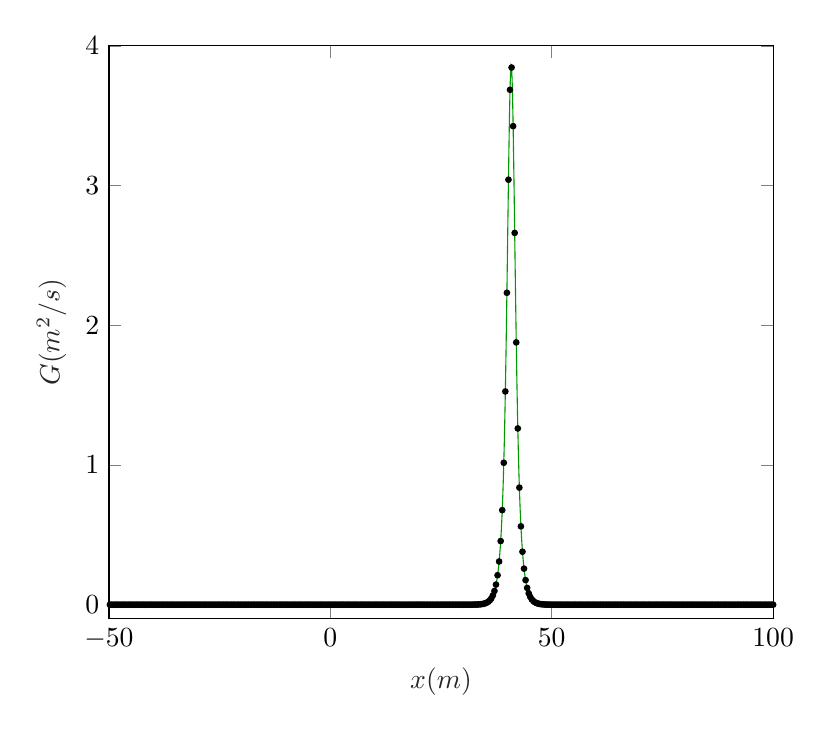
\begin{tikzpicture}

\begin{axis}[%
scale only axis,
xmin=-50,
xmax=100,
xtick={-50,   0,  50, 100},
xlabel style={font=\color{white!15!black}},
xlabel={$x (m)$},
ymin=-0.1,
ymax=4,
ytick={0, 1, 2, 3, 4},
ylabel style={font=\color{white!15!black}},
ylabel={$G (m^2/s)$},
axis background/.style={fill=white}
]
\addplot [color=green!60!black, forget plot]
  table[row sep=crcr]{%
-50.14064697609	-5.67925565028477e-44\\
-50.0234411626817	-6.46942449732437e-44\\
-49.9062353492733	-7.36953148507789e-44\\
-49.789029535865	-8.39487257823589e-44\\
-49.6718237224566	-9.56287190678446e-44\\
-49.5546179090483	-1.08933778628938e-43\\
-49.4374120956399	-1.2409000394494e-43\\
-49.3202062822316	-1.41354952273408e-43\\
-49.2030004688233	-1.61022015448423e-43\\
-49.0857946554149	-1.83425405633628e-43\\
-48.9685888420066	-2.08945834755365e-43\\
-48.8513830285982	-2.38016984129328e-43\\
-48.7341772151899	-2.71132874222405e-43\\
-48.6169714017815	-3.08856259787573e-43\\
-48.4997655883732	-3.51828193034678e-43\\
-48.3825597749648	-4.00778917348764e-43\\
-48.2653539615565	-4.56540276678192e-43\\
-48.1481481481481	-5.20059851471748e-43\\
-48.0309423347398	-5.92417061383291e-43\\
-47.9137365213315	-6.74841508385664e-43\\
-47.7965307079231	-7.68733872007089e-43\\
-47.6793248945148	-8.75689711773463e-43\\
-47.5621190811064	-9.97526581343133e-43\\
-47.4449132676981	-1.13631491509804e-42\\
-47.3277074542897	-1.29441321206272e-42\\
-47.2105016408814	-1.47450811504829e-42\\
-47.093295827473	-1.6796600661072e-42\\
-46.9760900140647	-1.91335531414344e-42\\
-46.8588842006564	-2.17956515847011e-42\\
-46.741678387248	-2.4828134350695e-42\\
-46.6244725738397	-2.82825339238234e-42\\
-46.5072667604313	-3.22175526301613e-42\\
-46.390060947023	-3.67000601952039e-42\\
-46.2728551336146	-4.18062300942952e-42\\
-46.1556493202063	-4.76228340062936e-42\\
-46.0384435067979	-5.42487163677648e-42\\
-45.9212376933896	-6.17964740855479e-42\\
-45.8040318799812	-7.03943699518549e-42\\
-45.6868260665729	-8.0188512277557e-42\\
-45.5696202531646	-9.13453377832024e-42\\
-45.4524144397562	-1.04054439940802e-41\\
-45.3352086263479	-1.18531790829781e-41\\
-45.2180028129395	-1.3502341125768e-41\\
-45.1007969995312	-1.53809551513841e-41\\
-44.9835911861228	-1.7520945380161e-41\\
-44.8663853727145	-1.99586777279541e-41\\
-44.7491795593061	-2.27355777901906e-41\\
-44.6319737458978	-2.58988348075698e-41\\
-44.5147679324894	-2.95022035762469e-41\\
-44.3975621190811	-3.36069179297554e-41\\
-44.2803563056728	-3.82827313159305e-41\\
-44.1631504922644	-4.36091021518543e-41\\
-44.0459446788561	-4.96765441001729e-41\\
-43.9287388654477	-5.65881642126743e-41\\
-43.8115330520394	-6.44614150795858e-41\\
-43.694327238631	-7.34300907597218e-41\\
-43.5771214252227	-8.36466004093106e-41\\
-43.4599156118143	-9.52845582464262e-41\\
-43.342709798406	-1.08541733863529e-40\\
-43.2255039849977	-1.23643413024305e-40\\
-43.1082981715893	-1.40846226056424e-40\\
-42.991092358181	-1.60442508898053e-40\\
-42.8738865447726	-1.827652709075e-40\\
-42.7566807313643	-2.081938538565e-40\\
-42.6394749179559	-2.3716037827318e-40\\
-42.5222691045476	-2.70157086680588e-40\\
-42.4050632911392	-3.07744708518192e-40\\
-42.2878574777309	-3.50561988895448e-40\\
-42.1706516643225	-3.99336543104426e-40\\
-42.0534458509142	-4.54897221347495e-40\\
-41.9362400375059	-5.18188193800127e-40\\
-41.8190342240975	-5.90284995363215e-40\\
-41.7018284106892	-6.72412802761265e-40\\
-41.5846225972808	-7.65967254578537e-40\\
-41.4674167838725	-8.72538168037957e-40\\
-41.3502109704641	-9.93936555554129e-40\\
-41.2330051570558	-1.13222540016589e-39\\
-41.1157993436474	-1.28975471283085e-39\\
-40.9985935302391	-1.46920146732771e-39\\
-40.8813877168308	-1.67361509139989e-39\\
-40.7641819034224	-1.90646928719458e-39\\
-40.6469760900141	-2.17172106160686e-39\\
-40.5297702766057	-2.47387796966146e-39\\
-40.4125644631974	-2.81807471363196e-39\\
-40.295358649789	-3.21016039958451e-39\\
-40.1781528363807	-3.65679793413976e-39\\
-40.0609470229723	-4.16557725055085e-39\\
-39.943741209564	-4.74514428820606e-39\\
-39.8265353961556	-5.40534791736657e-39\\
-39.7093295827473	-6.1574073059063e-39\\
-39.592123769339	-7.01410257219832e-39\\
-39.4749179559306	-7.98999196400849e-39\\
-39.3577121425223	-9.10165925402394e-39\\
-39.2405063291139	-1.03679955561304e-38\\
-39.1233005157056	-1.1810520351486e-38\\
-39.0060947022972	-1.3453747179742e-38\\
-38.8888888888889	-1.53256002097858e-38\\
-38.7716830754805	-1.74578887690003e-38\\
-38.6544772620722	-1.98868478949472e-38\\
-38.5372714486639	-2.26537540953428e-38\\
-38.4200656352555	-2.58056267802317e-38\\
-38.3028598218472	-2.93960272861585e-38\\
-38.1856540084388	-3.34859690705341e-38\\
-38.0684481950305	-3.81449545435936e-38\\
-37.9512423816221	-4.34521561573435e-38\\
-37.8340365682138	-4.94977618223231e-38\\
-37.7168307548054	-5.63845075155249e-38\\
-37.5996249413971	-6.42294231238227e-38\\
-37.4824191279887	-7.31658211909224e-38\\
-37.3652133145804	-8.3345562363561e-38\\
-37.2480075011721	-9.49416360348316e-38\\
-37.1308016877637	-1.08151100038787e-37\\
-37.0135958743554	-1.2319842935199e-37\\
-36.896390060947	-1.40339330708186e-37\\
-36.7791842475387	-1.59865087949707e-37\\
-36.6619784341303	-1.82107511958348e-37\\
-36.544772620722	-2.07444579282335e-37\\
-36.4275668073136	-2.36306855279352e-37\\
-36.3103609939053	-2.69184810927339e-37\\
-36.193155180497	-3.06637157641179e-37\\
-36.0759493670886	-3.49300341733039e-37\\
-35.9587435536803	-3.97899359860334e-37\\
-35.8415377402719	-4.53260079253712e-37\\
-35.7243319268636	-5.16323272088679e-37\\
-35.6071261134552	-5.88160602494042e-37\\
-35.4899203000469	-6.699928378722e-37\\
-35.3727144866385	-7.63210594005375e-37\\
-35.2555086732302	-8.69397966479689e-37\\
-35.1383028598218	-9.90359450007444e-37\\
-35.0210970464135	-1.12815060310125e-36\\
-34.9038912330052	-1.28511297919975e-36\\
-34.7866854195968	-1.46391391784721e-36\\
-34.6694796061885	-1.66759187211797e-36\\
-34.5522737927801	-1.89960804255711e-36\\
-34.4350679793718	-2.16390519507907e-36\\
-34.3178621659634	-2.46497466234507e-36\\
-34.2006563525551	-2.80793266720784e-36\\
-34.0834505391467	-3.19860726522513e-36\\
-33.9662447257384	-3.64363738370003e-36\\
-33.8490389123301	-4.15058564026676e-36\\
-33.7318330989217	-4.72806685820487e-36\\
-33.6146272855134	-5.38589446240624e-36\\
-33.497421472105	-6.13524724377348e-36\\
-33.3802156586967	-6.98885932596121e-36\\
-33.2630098452883	-7.96123656265768e-36\\
-33.14580403188	-9.06890304275518e-36\\
-33.0285982184716	-1.03306818923917e-35\\
-32.9113924050633	-1.17680151456735e-35\\
-32.7941865916549	-1.34053281198016e-35\\
-32.6769807782466	-1.52704444866057e-35\\
-32.5597749648383	-1.73950590940077e-35\\
-32.4425691514299	-1.98152765722979e-35\\
-32.3253633380216	-2.25722248780352e-35\\
-32.2081575246132	-2.57127542018214e-35\\
-32.0909517112049	-2.92902331168347e-35\\
-31.9737458977965	-3.33654554974806e-35\\
-31.8565400843882	-3.80076736198637e-35\\
-31.7393342709798	-4.32957750000788e-35\\
-31.6221284575715	-4.93196229689201e-35\\
-31.5049226441632	-5.61815837640502e-35\\
-31.3877168307548	-6.39982660902768e-35\\
-31.2705110173465	-7.29025027091278e-35\\
-31.1533052039381	-8.30456077318933e-35\\
-31.0360993905298	-9.45999479753952e-35\\
-30.9188935771214	-1.07761872076836e-34\\
-30.8016877637131	-1.22755047143627e-34\\
-30.6844819503047	-1.39834259639528e-34\\
-30.5672761368964	-1.59289745097464e-34\\
-30.450070323488	-1.81452120235933e-34\\
-30.3328645100797	-2.06698001292991e-34\\
-30.2156586966714	-2.3545640405285e-34\\
-30.098452883263	-2.68216034323976e-34\\
-29.9812470698547	-3.05533592759417e-34\\
-29.8640412564463	-3.48043235147226e-34\\
-29.746835443038	-3.96467348934472e-34\\
-29.6296296296296	-4.51628829115533e-34\\
-29.5124238162213	-5.14465062095144e-34\\
-29.3952180028129	-5.86043855160665e-34\\
-29.2780121894046	-6.67581582261175e-34\\
-29.1608063759962	-7.60463854453612e-34\\
-29.0436005625879	-8.66269066278986e-34\\
-28.9263947491796	-9.86795218204107e-34\\
-28.8091889357712	-1.12409047093557e-33\\
-28.6919831223629	-1.28048795083117e-33\\
-28.5747773089545	-1.45864539787368e-33\\
-28.4575714955462	-1.6615903299652e-33\\
-28.3403656821378	-1.89277149104129e-33\\
-28.2231598687295	-2.15611745728783e-33\\
-28.1059540553211	-2.45610339738575e-33\\
-27.9887482419128	-2.79782712127288e-33\\
-27.8715424285045	-3.18709570975801e-33\\
-27.7543366150961	-3.63052419712644e-33\\
-27.6371308016878	-4.13564798370029e-33\\
-27.5199249882794	-4.71105088863525e-33\\
-27.4027191748711	-5.36651101901884e-33\\
-27.2855133614627	-6.11316693409651e-33\\
-27.1683075480544	-6.96370692833562e-33\\
-27.051101734646	-7.93258464990982e-33\\
-26.9338959212377	-9.03626471871409e-33\\
-26.8166901078293	-1.02935025178213e-32\\
-26.699484294421	-1.17256629130129e-32\\
-26.5822784810127	-1.33570833165449e-32\\
-26.4650726676043	-1.52154872648717e-32\\
-26.347866854196	-1.73324555384564e-32\\
-26.2306610407876	-1.97439628296455e-32\\
-26.1134552273793	-2.24909890784659e-32\\
-25.9962494139709	-2.5620215865082e-32\\
-25.8790436005626	-2.91848196930506e-32\\
-25.7618377871542	-3.32453756440329e-32\\
-25.6446319737459	-3.78708867602171e-32\\
-25.5274261603376	-4.3139956647252e-32\\
-25.4102203469292	-4.91421252243247e-32\\
-25.2930145335209	-5.59793903204352e-32\\
-25.1758087201125	-6.37679409741217e-32\\
-25.0586029067042	-7.26401318914445e-32\\
-24.9413970932958	-8.27467326151825e-32\\
-24.8241912798875	-9.42594896264916e-32\\
-24.7069854664791	-1.07374044918077e-31\\
-24.5897796530708	-1.22313260635659e-31\\
-24.4725738396624	-1.39331006285001e-31\\
-24.3553680262541	-1.58716472862398e-31\\
-24.2381622128458	-1.80799087220775e-31\\
-24.1209563994374	-2.05954110183665e-31\\
-24.0037505860291	-2.34609013538603e-31\\
-23.8865447726207	-2.67250744277318e-31\\
-23.7693389592124	-3.04433999527589e-31\\
-23.652133145804	-3.46790652796809e-31\\
-23.5349273323957	-3.95040491712024e-31\\
-23.4177215189873	-4.50003449728256e-31\\
-23.300515705579	-5.12613539664557e-31\\
-23.1833098921707	-5.83934725847349e-31\\
-23.0661040787623	-6.65179004584142e-31\\
-22.948898265354	-7.5772700021819e-31\\
-22.8316924519456	-8.63151426763096e-31\\
-22.7144866385373	-9.83243813812407e-31\\
-22.5972808251289	-1.120044950891e-30\\
-22.4800750117206	-1.27587956760414e-30\\
-22.3628691983122	-1.45339583892122e-30\\
-22.2456633849039	-1.65561038692719e-30\\
-22.1284575714955	-1.88595954377831e-30\\
-22.0112517580872	-2.14835774699988e-30\\
-21.8940459446789	-2.44726405946538e-30\\
-21.7768401312705	-2.7877579444646e-30\\
-21.6596343178622	-3.17562558354374e-30\\
-21.5424285044538	-3.61745820395983e-30\\
-21.4252226910455	-4.12076408667597e-30\\
-21.3080168776371	-4.69409615830541e-30\\
-21.1908110642288	-5.34719733523786e-30\\
-21.0736052508204	-6.09116608985208e-30\\
-20.9563994374121	-6.93864505236433e-30\\
-20.8391936240038	-7.90403585331695e-30\\
-20.7219878105954	-9.0037438576331e-30\\
-20.6047819971871	-1.02564569491223e-29\\
-20.4875761837787	-1.16834631029645e-29\\
-20.3703703703704	-1.33090121428349e-29\\
-20.253164556962	-1.51607278301914e-29\\
-20.1359587435537	-1.72700772885597e-29\\
-20.0187529301453	-1.96729057399784e-29\\
-19.901547116737	-2.24100456406447e-29\\
-19.7843413033286	-2.55280105671022e-29\\
-19.6671354899203	-2.90797856445299e-29\\
-19.549929676512	-3.31257279492657e-29\\
-19.4327238631036	-3.77345921865547e-29\\
-19.3155180496953	-4.29846990733726e-29\\
-19.1983122362869	-4.89652662812327e-29\\
-19.0811064228786	-5.57779245563524e-29\\
-18.9639006094702	-6.35384447813479e-29\\
-18.8466947960619	-7.23787053272964e-29\\
-18.7294889826535	-8.24489331283325e-29\\
-18.6122831692452	-9.39202565624859e-29\\
-18.4950773558368	-1.06987613521126e-28\\
-18.3778715424285	-1.21873064085278e-28\\
-18.2606657290202	-1.38829564102781e-28\\
-18.1434599156118	-1.58145263792512e-28\\
-18.0262541022035	-1.80148404424055e-28\\
-17.9090482887951	-2.0521289628447e-28\\
-17.7918424753868	-2.3376467272134e-28\\
-17.6746366619784	-2.66288928239499e-28\\
-17.5574308485701	-3.03338363652019e-28\\
-17.4402250351617	-3.45542578399383e-28\\
-17.3230192217534	-3.93618769645192e-28\\
-17.2058134083451	-4.48383919963454e-28\\
-17.0886075949367	-5.10768680728865e-28\\
-16.9714017815284	-5.81833187137416e-28\\
-16.85419596812	-6.62785073609845e-28\\
-16.7369901547117	-7.54999995722585e-28\\
-16.6197843413033	-8.60045007405599e-28\\
-16.502578527895	-9.79705190667434e-28\\
-16.3853727144866	-1.11601399037952e-27\\
-16.2681669010783	-1.27128776961395e-27\\
-16.1509610876699	-1.44816517275059e-27\\
-16.0337552742616	-1.64965196527029e-27\\
-15.9165494608533	-1.87917211221926e-27\\
-15.7993436474449	-2.14062596334618e-27\\
-15.6821378340366	-2.4384565336808e-27\\
-15.5649320206282	-2.77772500589302e-27\\
-15.4477262072199	-3.16419673748154e-27\\
-15.3305203938115	-3.6044392343547e-27\\
-15.2133145804032	-4.10593375571712e-27\\
-15.0961087669948	-4.67720244681982e-27\\
-14.9789029535865	-5.32795316000339e-27\\
-14.8616971401782	-6.06924442504969e-27\\
-14.7444913267698	-6.91367337226614e-27\\
-14.6272855133615	-7.87558980177177e-27\\
-14.5100796999531	-8.97134003677153e-27\\
-14.3928738865448	-1.02195447047372e-26\\
-14.2756680731364	-1.16414151669705e-26\\
-14.1584622597281	-1.3261113973791e-26\\
-14.0412564463197	-1.51061654707431e-26\\
-13.9240506329114	-1.72079235334581e-26\\
-13.806844819503	-1.96021043796217e-26\\
-13.6896390060947	-2.23293935123833e-26\\
-13.5724331926864	-2.54361371092997e-26\\
-13.455227379278	-2.89751296059287e-26\\
-13.3380215658697	-3.30065108578702e-26\\
-13.2208157524613	-3.75987881271732e-26\\
-13.103609939053	-4.28300002602356e-26\\
-12.9864041256446	-4.87890438406459e-26\\
-12.8691983122363	-5.55771838529369e-26\\
-12.7519924988279	-6.33097745287205e-26\\
-12.6347866854196	-7.21182196183838e-26\\
-12.5175808720113	-8.21522054002271e-26\\
-12.4003750586029	-9.35822443736625e-26\\
-12.2831692451946	-1.06602572862732e-25\\
-12.1659634317862	-1.21434451770346e-25\\
-12.0487576183779	-1.38329926574592e-25\\
-11.9315518049695	-1.57576110462623e-25\\
-11.8143459915612	-1.79500063387508e-25\\
-11.6971401781528	-2.04474349960316e-25\\
-11.5799343647445	-2.32923370625412e-25\\
-11.4627285513361	-2.65330573707812e-25\\
-11.3455227379278	-3.0224667089047e-25\\
-11.2283169245195	-3.44298995731157e-25\\
-11.1111111111111	-3.9220216425292e-25\\
-10.9939052977028	-4.46770218768769e-25\\
-10.8766994842944	-5.08930461306618e-25\\
-10.7594936708861	-5.79739211712812e-25\\
-10.6422878574777	-6.60399758219424e-25\\
-10.5250820440694	-7.52282805518297e-25\\
-10.407876230661	-8.56949767825991e-25\\
-10.2906704172527	-9.76179302770403e-25\\
-10.1734646038444	-1.11199753700245e-24\\
-10.056258790436	-1.26671249717158e-24\\
-9.93905297702766	-1.44295333136797e-24\\
-9.82184716361932	-1.64371498754059e-24\\
-9.70464135021097	-1.87240910813395e-24\\
-9.58743553680262	-2.1329220058209e-24\\
-9.47022972339428	-2.42968070554245e-24\\
-9.35302390998594	-2.7677281751394e-24\\
-9.23581809657759	-3.15280902300708e-24\\
-9.11861228316924	-3.59146711907652e-24\\
-9.0014064697609	-4.09115679804335e-24\\
-8.88420065635255	-4.66036953457618e-24\\
-8.76699484294421	-5.30877824315931e-24\\
-8.64978902953587	-6.04740165472831e-24\\
-8.53258321612752	-6.88879156343276e-24\\
-8.41537740271917	-7.84724612550216e-24\\
-8.29817158931083	-8.93905283491006e-24\\
-8.18096577590249	-1.01827653048414e-23\\
-8.06375996249414	-1.15995185584475e-23\\
-7.94655414908579	-1.32133881867822e-23\\
-7.82934833567745	-1.50517994772675e-23\\
-7.7121425222691	-1.71459934652117e-23\\
-7.59493670886076	-1.95315578282238e-23\\
-7.47773089545242	-2.22490316452794e-23\\
-7.36052508204407	-2.53445942974058e-23\\
-7.24331926863572	-2.88708502168173e-23\\
-7.12611345522738	-3.28877228201366e-23\\
-7.00890764181904	-3.7463472816748e-23\\
-6.89170182841069	-4.26758581969034e-23\\
-6.77449601500234	-4.8613455611836e-23\\
-6.657290201594	-5.53771656007476e-23\\
-6.54008438818565	-6.30819272437408e-23\\
-6.42287857477731	-7.18586713786387e-23\\
-6.30567276136896	-8.18565455736856e-23\\
-6.18846694796062	-9.32454486661817e-23\\
-6.07126113455227	-1.06218917937732e-22\\
-5.95405532114393	-1.20997417989309e-22\\
-5.83684950773559	-1.37832087205614e-22\\
-5.71964369432724	-1.57009005474272e-22\\
-5.60243788091889	-1.78854055683312e-22\\
-5.48523206751055	-2.03738461610793e-22\\
-5.3680262541022	-2.32085096314685e-22\\
-5.25082044069386	-2.64375668224554e-22\\
-5.13361462728551	-3.0115890705196e-22\\
-5.01640881387717	-3.43059888626723e-22\\
-4.89920300046882	-3.90790657120676e-22\\
-4.78199718706048	-4.45162325167598e-22\\
-4.66479137365214	-5.07098857502693e-22\\
-4.54758556024379	-5.77652772353829e-22\\
-4.43037974683544	-6.58023027406032e-22\\
-4.31317393342709	-7.49575394284404e-22\\
-4.19596812001875	-8.53865667789042e-22\\
-4.07876230661041	-9.726661042881e-22\\
-3.96155649320206	-1.10799553854966e-21\\
-3.84435067979372	-1.26215369080274e-21\\
-3.72714486638537	-1.43776024702432e-21\\
-3.60993905297703	-1.637799376563e-21\\
-3.49273323956868	-1.86567044360962e-21\\
-3.37552742616034	-2.12524577427976e-21\\
-3.25832161275199	-2.42093646097287e-21\\
-3.14111579934364	-2.75776732225433e-21\\
-3.0239099859353	-3.14146229209073e-21\\
-2.90670417252696	-3.57854168950001e-21\\
-2.78949835911861	-4.07643302156808e-21\\
-2.67229254571027	-4.6435972027623e-21\\
-2.55508673230192	-5.28967233544967e-21\\
-2.43788091889358	-6.02563749495257e-21\\
-2.32067510548523	-6.86399930242403e-21\\
-2.20346929207689	-7.81900445606685e-21\\
-2.08626347866854	-8.90688183234557e-21\\
-1.96905766526019	-1.01461182713373e-20\\
-1.85185185185185	-1.15577727327786e-20\\
-1.73464603844351	-1.3165834161418e-20\\
-1.61744022503516	-1.4997629143058e-20\\
-1.50023441162681	-1.70842862787873e-20\\
-1.38302859821847	-1.94612651687457e-20\\
-1.26582278481013	-2.21689589947048e-20\\
-1.14861697140178	-2.52533809414499e-20\\
-1.03141115799344	-2.87669461216609e-20\\
-0.914205344585092	-3.2769362291932e-20\\
-0.796999531176745	-3.73286444963069e-20\\
-0.679793717768398	-4.2522270879673e-20\\
-0.562587904360058	-4.84384993123216e-20\\
-0.445382090951711	-5.51778671997359e-20\\
-0.328176277543363	-6.28548999646078e-20\\
-0.210970464135023	-7.16000572341759e-20\\
-0.0937646507266763	-8.15619498054077e-20\\
0.0234411626816708	-9.29098650620153e-20\\
0.140646976090011	-1.05836643758969e-19\\
0.257852789498358	-1.2056195706114e-19\\
0.375058602906705	-1.37336039524405e-19\\
0.492264416315052	-1.56443941455628e-19\\
0.609470229723392	-1.7821037291397e-19\\
0.726676043131739	-2.03005221670051e-19\\
0.843881856540087	-2.3124983889238e-19\\
0.961087669948427	-2.63424199376843e-19\\
1.07829348335677	-3.0007505799658e-19\\
1.19549929676512	-3.41825240978853e-19\\
1.31270511017347	-3.89384229900186e-19\\
1.42991092358181	-4.43560218258835e-19\\
1.54711673699016	-5.0527384550797e-19\\
1.6643225503985	-5.75573841938713e-19\\
1.78152836380684	-6.55654850274386e-19\\
1.89873417721519	-7.468777268271e-19\\
2.01593999062354	-8.50792667204355e-19\\
2.13314580403188	-9.69165549552229e-19\\
2.25035161744022	-1.10400794299894e-18\\
2.36755743084857	-1.25761129124728e-18\\
2.48476324425692	-1.43258585221445e-18\\
2.60196905766526	-1.63190505544009e-18\\
2.71917487107361	-1.85895603104999e-18\\
2.83638068448195	-2.11759716893897e-18\\
2.95358649789029	-2.41222368630501e-18\\
3.07079231129864	-2.74784231775607e-18\\
3.18799812470699	-3.13015639723567e-18\\
3.30520393811533	-3.56566277760675e-18\\
3.42240975152367	-4.06176223489603e-18\\
3.53961556493202	-4.62688523335374e-18\\
3.65682137834037	-5.27063518851562e-18\\
3.77402719174871	-6.00395166280868e-18\\
3.89123300515705	-6.83929626696383e-18\\
4.0084388185654	-7.79086442635072e-18\\
4.12564463197375	-8.87482661088508e-18\\
4.24285044538209	-1.01096031278477e-17\\
4.36005625879044	-1.15161771473073e-17\\
4.47726207219878	-1.31184512795408e-17\\
4.59446788560712	-1.49436537639508e-17\\
4.71167369901547	-1.70228011720496e-17\\
4.82887951242382	-1.93912254874488e-17\\
4.94608532583216	-2.20891745197898e-17\\
5.0632911392405	-2.51624958557439e-17\\
5.18049695264885	-2.86634159698041e-17\\
5.2977027660572	-3.26514277346808e-17\\
5.41490857946554	-3.71943014132084e-17\\
5.53211439287389	-4.23692363120529e-17\\
5.64932020628223	-4.82641726678348e-17\\
5.76652601969058	-5.49792860592091e-17\\
5.88373183309892	-6.262868974018e-17\\
6.00093764650727	-7.13423738232549e-17\\
6.11814345991561	-8.12684142659256e-17\\
6.23534927332395	-9.25754891988914e-17\\
6.3525550867323	-1.0545574535724e-16\\
6.46976090014065	-1.20128063325257e-16\\
6.58696671354899	-1.36841777082808e-16\\
6.70417252695734	-1.55880911061387e-16\\
6.82137834036568	-1.77569006712211e-16\\
6.93858415377403	7.04499652447659e-16\\
7.05578996718237	6.76356685553378e-16\\
7.17299578059072	6.44298118257833e-16\\
7.29020159399906	6.07779163419e-16\\
7.4074074074074	5.66179236316026e-16\\
7.52461322081575	5.187914087451e-16\\
7.6418190342241	4.6481039583772e-16\\
7.75902484763245	4.03318871455313e-16\\
7.87623066104079	1.2400461526653e-15\\
7.99343647444913	1.16025335006822e-15\\
8.11064228785748	1.06935877802938e-15\\
8.22784810126582	9.6581781998282e-16\\
8.34505391467417	1.75464522610409e-15\\
8.46225972808251	1.62028812064766e-15\\
8.57946554149086	1.46723757970471e-15\\
8.6966713548992	2.19966701254122e-15\\
8.81387716830755	2.00106514466603e-15\\
8.9310829817159	2.68160558209758e-15\\
9.04828879512424	3.33066954795203e-15\\
9.16549460853258	3.03710337004486e-15\\
9.28270042194093	3.60946687875131e-15\\
9.39990623534927	4.13530299295864e-15\\
9.51711204875762	5.51491251456027e-15\\
9.63431786216596	5.92737275627671e-15\\
9.75152367557431	6.27105786754127e-15\\
9.86872948898265	7.4431732678683e-15\\
9.985935302391	8.52604449246784e-15\\
10.1031411157993	9.50725477904178e-15\\
10.2203469292077	1.12794340635809e-14\\
10.337552742616	1.2919695799463e-14\\
10.4547585560244	1.44096859727564e-14\\
10.5719643694327	1.66352712033538e-14\\
10.6891701828411	1.8665860631684e-14\\
10.8063759962494	2.13810982838562e-14\\
10.9235818096578	2.38433049416946e-14\\
11.0407876230661	2.78308243249419e-14\\
11.1579934364744	3.14900049267945e-14\\
11.2751992498828	3.56819384357729e-14\\
11.3924050632911	4.03545863366771e-14\\
11.5096108766995	4.63554441403836e-14\\
11.6268166901078	5.27102112112611e-14\\
11.7440225035162	6.02487403504022e-14\\
11.8612283169245	6.88834078117178e-14\\
11.9784341303329	7.85143985411919e-14\\
12.0956399437412	8.90280099701405e-14\\
12.2128457571496	1.01201494084096e-13\\
12.3300515705579	1.15794082113248e-13\\
12.4472573839662	1.31730928714194e-13\\
12.5644631973746	1.49727352947061e-13\\
12.6816690107829	1.71378810509016e-13\\
12.7988748241913	1.94623316208983e-13\\
12.9160806375996	2.21898190617956e-13\\
13.033286451008	2.52881056686928e-13\\
13.1504922644163	2.88111458525937e-13\\
13.2676980778247	3.28077846606643e-13\\
13.384903891233	3.73210468978376e-13\\
13.5021097046413	4.2568682196768e-13\\
13.6193155180497	4.84888554293072e-13\\
13.736521331458	5.51924830480177e-13\\
13.8537271448664	6.28713586641477e-13\\
13.9709329582747	7.17061120847776e-13\\
14.0881387716831	8.15926237832966e-13\\
14.2053445850914	9.29563523903678e-13\\
14.3225503984998	1.05934222318704e-12\\
14.4397562119081	1.20644360089922e-12\\
14.5569620253165	1.37455511219495e-12\\
14.6741678387248	1.56621351223959e-12\\
14.7913736521331	1.78367769249551e-12\\
14.9085794655415	2.0316103436789e-12\\
15.0257852789498	2.31431359423626e-12\\
15.1429910923582	2.63658561869945e-12\\
15.2601969057665	3.00366349205996e-12\\
15.3774027191749	3.42115809333096e-12\\
15.4946085325832	3.89770027490109e-12\\
15.6118143459916	4.43941574627565e-12\\
15.7290201593999	5.05708304503515e-12\\
15.8462259728083	5.76058328019619e-12\\
15.9634317862166	6.56240236785392e-12\\
16.0806375996249	7.47567524890499e-12\\
16.1978434130333	8.51583741453226e-12\\
16.3150492264416	9.70044034047623e-12\\
16.43225503985	1.10498480164934e-11\\
16.5494608532583	1.25869974496629e-11\\
16.6666666666667	1.43389393944725e-11\\
16.783872480075	1.63338072536351e-11\\
16.9010782934834	1.86059037082805e-11\\
17.0182841068917	2.11943906731916e-11\\
17.1354899203	2.41437366925726e-11\\
17.2526957337084	2.75022868728026e-11\\
17.3699015471167	3.13289209766071e-11\\
17.4871073605251	3.56878405148137e-11\\
17.6043131739334	4.06532358790363e-11\\
17.7215189873418	4.63093119822287e-11\\
17.8387248007501	5.27529116277478e-11\\
17.9559306141585	6.00923721301736e-11\\
18.0731364275668	6.84534770491427e-11\\
18.1903422409752	7.79779725144793e-11\\
18.3075480543835	8.88264109953478e-11\\
18.4247538677918	1.01185293792682e-10\\
18.5419596812002	1.15263971149788e-10\\
18.6591654946085	1.31300304972158e-10\\
18.7763713080169	1.49568704282621e-10\\
18.8935771214252	1.70378696985551e-10\\
19.0107829348336	1.94083931884914e-10\\
19.1279887482419	2.21087039813816e-10\\
19.2451945616503	2.51847536584693e-10\\
19.3624003750586	2.86887245683508e-10\\
19.4796061884669	3.26803122464384e-10\\
19.5968120018753	3.72271959015278e-10\\
19.7140178152836	4.2406679836046e-10\\
19.831223628692	4.8306859894736e-10\\
19.9484294421003	5.50279340645031e-10\\
20.0656352555087	6.2684092820148e-10\\
20.182841068917	7.14054248834957e-10\\
20.3000468823254	8.134026869523e-10\\
20.4172526957337	9.26573485573149e-10\\
20.5344585091421	1.05548934970686e-09\\
20.6516643225504	1.20234269621174e-09\\
20.7688701359587	1.36962762750629e-09\\
20.8860759493671	1.56018732177038e-09\\
21.0032817627754	1.77726001323682e-09\\
21.1204875761838	2.02453477599012e-09\\
21.2376933895921	2.30621282957294e-09\\
21.3548992030005	2.62708178169132e-09\\
21.4721050164088	2.99259470439821e-09\\
21.5893108298172	3.40896123711507e-09\\
21.7065166432255	3.88325868200008e-09\\
21.8237224566338	4.42354642090899e-09\\
21.9409282700422	5.039004893022e-09\\
22.0581340834505	5.74009387675532e-09\\
22.1753398968589	6.53872731321492e-09\\
22.2925457102672	7.44847706538602e-09\\
22.4097515236756	8.48480229793672e-09\\
22.5269573370839	9.66531352227517e-09\\
22.6441631504923	1.10100718088318e-08\\
22.7613689639006	1.25419304879271e-08\\
22.878574777309	1.42869207246381e-08\\
22.9957805907173	1.62746953904763e-08\\
23.1129864041256	1.85390327705267e-08\\
23.230192217534	2.11184149675598e-08\\
23.3473980309423	2.40566719078874e-08\\
23.4646038443507	2.74037357635419e-08\\
23.581809657759	3.12164851421731e-08\\
23.6990154711674	3.55597115697239e-08\\
23.8162212845757	4.05072217045498e-08\\
23.9334270979841	4.61430921092188e-08\\
24.0506329113924	5.25630938509119e-08\\
24.1678387248007	5.98763261550833e-08\\
24.2850445382091	6.82070678624435e-08\\
24.4022503516174	7.76968853896477e-08\\
24.5194561650258	8.85070437070075e-08\\
24.6366619784341	1.00821247029413e-07\\
24.7538677918425	1.1484875460448e-07\\
24.8710736052508	1.30827945090361e-07\\
24.9882794186592	1.49030359311305e-07\\
25.1054852320675	1.69765320102649e-07\\
25.2226910454759	1.93385186342083e-07\\
25.3398968588842	2.20291342766761e-07\\
25.4571026722925	2.50941018476639e-07\\
25.5743084857009	2.85855058826503e-07\\
25.6915142991092	3.25626774548931e-07\\
25.8087201125176	3.70932027150908e-07\\
25.9259259259259	4.22540709487775e-07\\
26.0431317393343	4.81329833101205e-07\\
26.1603375527426	5.4829843077014e-07\\
26.277543366151	6.24584532254987e-07\\
26.3947491795593	7.1148450277315e-07\\
26.5119549929676	8.10475075926028e-07\\
26.629160806376	9.23238446084501e-07\\
26.7463666197843	1.05169085352027e-06\\
26.8635724331927	1.19801515152588e-06\\
26.980778246601	1.3646978958533e-06\\
27.0979840600094	1.55457160478368e-06\\
27.2151898734177	1.77086288830396e-06\\
27.3323956868261	2.01724728352007e-06\\
27.4496015002344	2.29791170841468e-06\\
27.5668073136428	2.61762561877808e-06\\
27.6840131270511	2.98182205022739e-06\\
27.8012189404594	3.39668994642382e-06\\
27.9184247538678	3.86927932937337e-06\\
28.0356305672761	4.40762109996003e-06\\
28.1528363806845	5.02086350780401e-06\\
28.2700421940928	5.71942760981789e-06\\
28.3872480075012	6.51518435488633e-06\\
28.5044538209095	7.42165630450217e-06\\
28.6216596343179	8.454247420254e-06\\
28.7388654477262	9.63050481972133e-06\\
28.8560712611346	1.09704169509731e-05\\
28.9732770745429	1.24967532438382e-05\\
29.0904828879512	1.42354510177999e-05\\
29.2076887013596	1.62160562181099e-05\\
29.3248945147679	1.84722254612266e-05\\
29.4421003281763	2.10422979253289e-05\\
29.5593061415846	2.39699467943057e-05\\
29.676511954993	2.73049213320218e-05\\
29.7937177684013	3.11038921735575e-05\\
29.9109235818097	3.543141420647e-05\\
30.028129395218	4.03610233869567e-05\\
30.1453352086263	4.59764861124935e-05\\
30.2625410220347	5.23732223738739e-05\\
30.379746835443	5.96599268373539e-05\\
30.4969526488514	6.79604153903211e-05\\
30.6141584622597	7.74157284720337e-05\\
30.7313642756681	8.81865268958671e-05\\
30.8485700890764	0.000100455820813016\\
30.9657759024848	0.000114432078097946\\
31.0829817158931	0.000130352764879346\\
31.2001875293015	0.000148488378236566\\
31.3173933427098	0.000169147039410214\\
31.4345991561181	0.000192679725343126\\
31.5518049695265	0.000219486227146894\\
31.6690107829348	0.000250021936355717\\
31.7862165963432	0.000284805573764508\\
31.9034224097515	0.000324427991524394\\
32.0206282231599	0.00036956219721324\\
32.1378340365682	0.00042097476908627\\
32.2550398499766	0.000479538855050475\\
32.3722456633849	0.000546248974354167\\
32.4894514767932	0.000622237871096495\\
32.6066572902016	0.000708795702770705\\
32.7238631036099	0.000807391885842149\\
32.8410689170183	0.000919699964270065\\
32.9582747304266	0.00104762591672266\\
33.075480543835	0.00119334037464924\\
33.1926863572433	0.00135931528724505\\
33.3098921706517	0.00154836564156118\\
33.42709798406	0.00176369692761302\\
33.5443037974684	0.00200895913045486\\
33.6615096108767	0.00228830813496124\\
33.778715424285	0.0026064755459206\\
33.8959212376934	0.00296884805739681\\
34.0131270511017	0.00338155765261079\\
34.1303328645101	0.0038515840807093\\
34.2475386779184	0.0043868712411525\\
34.3647444913268	0.00499645931221381\\
34.4819503047351	0.00569063468894814\\
34.5991561181435	0.00648110004999354\\
34.7163619315518	0.00738116715395361\\
34.8335677449601	0.00840597527687077\\
34.9507735583685	0.00957273854516631\\
35.0679793717768	0.0109010257960637\\
35.1851851851852	0.0124130770137129\\
35.3023909985935	0.0141341608487715\\
35.4195968120019	0.0160929782392172\\
35.5368026254102	0.0183221177212166\\
35.6540084388186	0.0208585686674843\\
35.7712142522269	0.0237442994420471\\
35.8884200656353	0.0270269083544166\\
36.0056258790436	0.0307603563934693\\
36.122831692452	0.035005792114396\\
36.2400375058603	0.0398324808794348\\
36.3572433192686	0.0453188531192728\\
36.474449132677	0.0515536896839815\\
36.5916549460853	0.058637467113298\\
36.7088607594937	0.0666838923661058\\
36.826066572902	0.0758216660114743\\
36.9432723863104	0.0861965261589085\\
37.0604781997187	0.0979736438396166\\
37.177684013127	0.111340465761539\\
37.2948898265354	0.126510134136342\\
37.4120956399437	0.143725657307186\\
37.5293014533521	0.163265060239153\\
37.6465072667604	0.18544780997582\\
37.7637130801688	0.210642884009107\\
37.8809188935771	0.239278919318419\\
37.9981247069855	0.271856927019288\\
38.1153305203938	0.308966047623336\\
38.2325363338022	0.351302699209388\\
38.3497421472105	0.399693152289034\\
38.4669479606189	0.455118936508369\\
38.5841537740272	0.518743403174827\\
38.7013595874355	0.591936081115553\\
38.8185654008439	0.676289050626706\\
38.9357712142522	0.773616410414419\\
39.0529770276606	0.885924245950563\\
39.1701828410689	1.01533493398509\\
39.2873886544773	1.16394729396258\\
39.4045944678856	1.33361480679152\\
39.5218002812939	1.5256301458044\\
39.6390060947023	1.74031788213731\\
39.7562119081106	1.97655972760745\\
39.873417721519	2.23130695402441\\
39.9906235349273	2.4991677259524\\
40.1078293483357	2.7721835271631\\
40.225035161744	3.03991577737864\\
40.3422409751524	3.28993855737342\\
40.4594467885607	3.5087697683505\\
40.5766526019691	3.6831771393487\\
40.6938584153774	3.80168867345452\\
40.8110642287858	3.85605242448379\\
40.9282700421941	3.84236156950501\\
41.0454758556024	3.76160713576826\\
41.1626816690108	3.61953661767913\\
41.2798874824191	3.42584992208795\\
41.3970932958275	3.1929075462474\\
41.5142991092358	2.93421649157851\\
41.6315049226442	2.66297480376634\\
41.7487107360525	2.39090093158618\\
41.8659165494608	2.12747622706502\\
41.9831223628692	1.87962296362839\\
42.1003281762775	1.65175555341958\\
42.2175339896859	1.44609450039702\\
42.3347398030942	1.2631215430121\\
42.4519456165026	1.10207080682944\\
42.5691514299109	0.961381300553836\\
42.6863572433193	0.83906894293178\\
42.8035630567276	0.733003824786157\\
42.920768870136	0.641097321765158\\
43.0379746835443	0.56141401545166\\
43.1551804969527	0.492226988879258\\
43.272386310361	0.432034306362408\\
43.3895921237693	0.379551484780163\\
43.5067979371777	0.333691047614705\\
43.624003750586	0.293536745663719\\
43.7412095639944	0.258317163049273\\
43.8584153774027	0.227381314611746\\
43.9756211908111	0.200177414040275\\
44.0928270042194	0.176235110326417\\
44.2100328176277	0.155151001248085\\
44.3272386310361	0.136577004334741\\
44.4444444444444	0.12021109647153\\
44.5616502578528	0.105789951555873\\
44.6788560712611	0.0930830650285291\\
44.7960618846695	0.0818880268273618\\
44.9132676980778	0.0720266752115634\\
45.0304735114862	0.0633419258984559\\
45.1476793248945	0.0556951217173727\\
45.2648851383029	0.0489637877354776\\
45.3820909517112	0.0430397069430314\\
45.4992967651196	0.0378272538771574\\
45.6165025785279	0.0332419397537066\\
45.7337083919362	0.0292091342818248\\
45.8509142053446	0.0256629375853651\\
45.9681200187529	0.0225451815022948\\
46.0853258321613	0.019804543690133\\
46.2025316455696	0.0173957609502312\\
46.319737458978	0.01527893036459\\
46.4369432723863	0.013418888472188\\
46.5541490857947	0.0117846599728802\\
46.671354899203	0.0103489684539457\\
46.7885607126113	0.00908780246542502\\
46.9057665260197	0.00798003097695619\\
47.022972339428	0.00700706286391573\\
47.1401781528364	0.00615254561573114\\
47.2573839662447	0.00540209894801401\\
47.3745897796531	0.00474307944168806\\
47.4917955930614	0.00416437273252394\\
47.6090014064698	0.00365621013788339\\
47.7262072198781	0.00321000693714024\\
47.8434130332865	0.0028182198210215\\
47.9606188466948	0.00247422129522856\\
48.0778246601031	0.00217218906745937\\
48.1950304735115	0.00190700866629904\\
48.3122362869198	0.00167418773745018\\
48.4294421003282	0.00146978063920566\\
48.5466479137365	0.00129032211684926\\
48.6638537271449	0.00113276897642273\\
48.7810595405532	0.000994448803638677\\
48.8982653539616	0.000873014885194374\\
49.0154711673699	0.000766406588715388\\
49.1326769807782	0.000672814545294697\\
49.2498827941866	0.000590650056332495\\
49.3670886075949	0.000518518215142778\\
49.4842944210033	0.000455194294565743\\
49.6015002344116	0.000399603005533313\\
49.71870604782	0.000350800278896128\\
49.8359118612283	0.000307957264620689\\
49.9531176746367	0.000270346279304261\\
50.070323488045	0.000237328465416525\\
50.1875293014534	0.00020834295424856\\
50.3047351148617	0.000182897349733278\\
50.42194092827	0.000160559372434788\\
50.5391467416784	0.000140949522488123\\
50.6563525550867	0.000123734637420259\\
50.7735583684951	0.000108622235832875\\
50.8907641819034	9.535555118558e-05\\
51.0079699953118	8.37091715792946e-05\\
51.1251758087201	7.34852116298702e-05\\
51.2423816221285	6.45099515715433e-05\\
51.3595874355368	5.66308865882875e-05\\
51.4767932489451	4.97141363256311e-05\\
51.5939990623535	4.36421706561349e-05\\
51.7112048757618	3.83118130820918e-05\\
51.8284106891702	3.36324879188859e-05\\
51.9456165025785	2.95246814844171e-05\\
52.0628223159869	2.59185911857115e-05\\
52.1800281293952	2.27529395618496e-05\\
52.2972339428036	1.99739331440549e-05\\
52.4144397562119	1.75343484536477e-05\\
52.5316455696203	1.53927296169867e-05\\
52.6488513830286	1.35126839663297e-05\\
52.7660571964369	1.18622636660737e-05\\
52.8832630098453	1.04134228530748e-05\\
53.0004688232536	9.14154108096375e-06\\
53.117674636662	8.02500495672601e-06\\
53.2348804500703	7.04484087936342e-06\\
53.3520862634787	6.18439262930557e-06\\
53.469292076887	5.42903832928282e-06\\
53.5864978902954	4.76594198592767e-06\\
53.7037037037037	4.18383536191298e-06\\
53.820909517112	3.67282649856413e-06\\
53.9381153305204	3.2242316211661e-06\\
54.0553211439287	2.83042757603355e-06\\
54.1725269573371	2.48472228533345e-06\\
54.2897327707454	2.18124103377709e-06\\
54.4069385841538	1.91482662996269e-06\\
54.5241443975621	1.68095177710319e-06\\
54.6413502109705	1.47564213539028e-06\\
54.7585560243788	1.29540878420287e-06\\
54.8757618377872	1.13718893501548e-06\\
54.9929676511955	9.98293884916949e-07\\
55.1101734646038	8.76363324924987e-07\\
55.2273792780122	7.69325232120056e-07\\
55.3445850914205	6.75360656522762e-07\\
55.4617909048289	5.92872813615988e-07\\
55.5789967182372	5.20459948363709e-07\\
55.6962025316456	4.56891513642067e-07\\
55.8134083450539	4.01087259981465e-07\\
55.9306141584623	3.52098879619226e-07\\
56.0478199718706	3.09093888214549e-07\\
56.165025785279	2.71341482066949e-07\\
56.2822315986873	2.38200114739226e-07\\
56.3994374120956	2.0910659940463e-07\\
56.516643225504	1.83566535170887e-07\\
56.6338490389123	1.61145909163934e-07\\
56.7510548523207	1.41463714063882e-07\\
56.868260665729	1.24185482935527e-07\\
56.9854664791374	1.09017595302862e-07\\
57.1026722925457	9.57022992092983e-08\\
57.2198781059541	8.40133195531076e-08\\
57.3370839193624	7.37520191109097e-08\\
57.4542897327707	6.47440233324812e-08\\
57.5714955461791	5.68362552085657e-08\\
57.6887013595874	4.98943338506582e-08\\
57.8059071729958	4.38002911038125e-08\\
57.9231129864041	3.84505689756135e-08\\
58.0403187998125	3.37542555331405e-08\\
58.1575246132208	2.96315457442955e-08\\
58.2747304266292	2.60123798993602e-08\\
58.3919362400375	2.28352544360361e-08\\
58.5091420534459	2.00461798853552e-08\\
58.6263478668542	1.75977598328886e-08\\
58.7435536802625	1.54483882075069e-08\\
58.8607594936709	1.35615373008148e-08\\
58.9779653070792	1.19051458347005e-08\\
59.0951711204876	1.0451063227664e-08\\
59.2123769338959	9.17458102442933e-09\\
59.3295827473043	8.05400685282222e-09\\
59.4467885607126	7.07029950451201e-09\\
59.563994374121	6.20673960097379e-09\\
59.6812001875293	5.4486551091703e-09\\
59.7984060009376	4.78316246774925e-09\\
59.915611814346	4.19895167988948e-09\\
60.0328176277543	3.68609621434977e-09\\
60.1500234411627	3.23588002627275e-09\\
60.267229254571	2.84065277233825e-09\\
60.3844350679794	2.49369866006619e-09\\
60.5016408813877	2.18912047782917e-09\\
60.6188466947961	1.92174379033749e-09\\
60.7360525082044	1.68702435595214e-09\\
60.8532583216128	1.48097250693703e-09\\
60.9704641350211	1.30008815693701e-09\\
61.0876699484294	1.1412963606888e-09\\
61.2048757618378	1.00189954894581e-09\\
61.3220815752461	8.79528924496902e-10\\
61.4392873886545	7.72103725720905e-10\\
61.5564932020628	6.77799743300379e-10\\
61.6736990154712	5.95013908843853e-10\\
61.7909048288795	5.22339832825461e-10\\
61.9081106422879	4.58541920950951e-10\\
62.0253164556962	4.02535607526243e-10\\
62.1425222691045	3.53370328379264e-10\\
62.2597280825129	3.10210011845675e-10\\
62.3769338959212	2.72321254724056e-10\\
62.4941397093296	2.39060284348352e-10\\
62.6113455227379	2.09861575362766e-10\\
62.7285513361463	1.84229158127154e-10\\
62.8457571495546	1.61728012687034e-10\\
62.962962962963	1.41974741835604e-10\\
63.0801687763713	1.24633958738684e-10\\
63.1973745897797	1.09411398676312e-10\\
63.314580403188	9.60483566279749e-11\\
63.4317862165964	8.43166034949625e-11\\
63.5489920300047	7.40183671234426e-11\\
63.666197843413	6.49778224194803e-11\\
63.7834036568214	5.70413595656553e-11\\
63.9006094702297	5.0074877650217e-11\\
64.0178152836381	4.39581347643837e-11\\
64.1350210970464	3.85897834444105e-11\\
64.2522269104548	3.38759121629375e-11\\
64.3694327238631	2.97383848501277e-11\\
64.4866385372714	2.61067259171765e-11\\
64.6038443506798	2.29180498783875e-11\\
64.7210501640881	2.01187023652085e-11\\
64.8382559774965	1.76612775896127e-11\\
64.9554617909048	1.55042774043464e-11\\
65.0726676043132	1.36107944784585e-11\\
65.1898734177215	1.19480415777351e-11\\
65.3070792311299	1.04886411344084e-11\\
65.4242850445382	9.20733419125833e-12\\
65.5414908579466	8.08308894762876e-12\\
65.6586966713549	7.09573262911721e-12\\
65.7759024847633	6.22889914723999e-12\\
65.8931082981716	5.46841512104384e-12\\
66.0103141115799	4.80066152342425e-12\\
66.1275199249883	4.21454102641495e-12\\
66.2447257383966	3.69979946481011e-12\\
66.361931551805	3.24714435808487e-12\\
66.4791373652133	2.85106927898996e-12\\
66.5963431786217	2.50269099709875e-12\\
66.71354899203	2.19708385482667e-12\\
66.8307548054383	1.92881628457429e-12\\
66.9479606188467	1.69291937432852e-12\\
67.065166432255	1.48675466040801e-12\\
67.1823722456634	1.30462110069318e-12\\
67.2995780590717	1.1450510715596e-12\\
67.4167838724801	1.00540641924392e-12\\
67.5339896858884	8.82817448986705e-13\\
67.6511954992968	7.75117979484482e-13\\
67.7684013127051	6.79963394683483e-13\\
67.8856071261135	5.9757276043556e-13\\
68.0028129395218	5.24400536546676e-13\\
68.1200187529302	4.60407566163365e-13\\
68.2372245663385	4.03635173987748e-13\\
68.3544303797468	3.54751980697062e-13\\
68.4716361931552	3.11624619508301e-13\\
68.5888420065635	2.7295480770559e-13\\
68.7060478199719	2.40101651354246e-13\\
68.8232536333802	2.10741912087993e-13\\
68.9404594467886	1.85224174873487e-13\\
69.0576652601969	1.6204090032236e-13\\
69.1748710736052	1.42367496221956e-13\\
69.2920768870136	1.25533011192667e-13\\
69.4092827004219	1.09930916416431e-13\\
69.5264885138303	9.66497207179167e-14\\
69.6436943272386	8.49421875046714e-14\\
69.760900140647	7.40415944161942e-14\\
69.8781059540553	6.49776618416961e-14\\
69.9953117674637	5.69515451122389e-14\\
70.112517580872	5.00579914212206e-14\\
70.2297233942804	4.43801756373891e-14\\
70.3469292076887	3.9084339463609e-14\\
70.4641350210971	3.42345807796795e-14\\
70.5813408345054	2.98871686163569e-14\\
70.6985466479137	2.60914993629177e-14\\
70.8157524613221	2.28909361845109e-14\\
70.9329582747304	2.03235459139431e-14\\
71.0501640881388	1.75159716672008e-14\\
71.1673699015471	1.54043235408897e-14\\
71.2845757149555	1.40143543112772e-14\\
71.4017815283638	1.15551227909443e-14\\
71.5189873417721	1.07667979182304e-14\\
71.6361931551805	8.94647900858701e-15\\
71.7533989685888	7.92300882115332e-15\\
71.8706047819972	6.80303927647333e-15\\
71.9878105954055	6.50513097973754e-15\\
72.1050164088139	5.2260821465019e-15\\
72.2222222222222	4.78852434172306e-15\\
72.3394280356306	4.29365692062473e-15\\
72.4566338490389	3.74847962073704e-15\\
72.5738396624473	3.15913723885505e-15\\
72.6910454758556	2.53102405262023e-15\\
72.8082512892639	2.77564976121125e-15\\
72.9254571026723	2.08362286457273e-15\\
73.0426629160806	2.27214121754178e-15\\
73.159868729489	1.53085985992756e-15\\
73.2770745428973	1.67613964107101e-15\\
73.3942803563057	8.96900826274584e-16\\
73.511486169714	1.0088592349742e-15\\
73.6286919831224	1.10714315891012e-15\\
73.7458977965307	1.19342278557182e-15\\
73.8631036099391	3.62390034414175e-16\\
73.9803094233474	4.28880564811534e-16\\
74.0975152367557	4.87250010286301e-16\\
74.2147210501641	5.38490271789258e-16\\
74.3319268635724	5.83472100510359e-16\\
74.4491326769808	6.2295989498576e-16\\
74.5663384903891	6.57624690901446e-16\\
74.6835443037975	6.88055564335636e-16\\
74.8007501172058	7.14769642220877e-16\\
74.9179559306142	-1.68553382915683e-16\\
75.0351617440225	-1.4796644627268e-16\\
75.1523675574308	-1.29893976874485e-16\\
75.2695733708392	-1.14028860280767e-16\\
75.3867791842475	-1.00101492692729e-16\\
75.5039849976559	-8.78751994419661e-17\\
75.6211908110642	-7.71422130603886e-17\\
75.7383966244726	-6.77201425845335e-17\\
75.8556024378809	-5.94488740954261e-17\\
75.9728082512893	-5.2187849823296e-17\\
76.0900140646976	-4.58136795796512e-17\\
76.207219878106	-4.02180439265778e-17\\
76.3244256915143	-3.53058534507796e-17\\
76.4416315049226	-3.09936328619949e-17\\
76.558837318331	-2.72081024559658e-17\\
76.6760431317393	-2.38849328360626e-17\\
76.7932489451477	-2.09676517319247e-17\\
76.910454758556	-1.84066843381488e-17\\
77.0276605719644	-1.61585108650196e-17\\
77.1448663853727	-1.41849269851291e-17\\
77.2620721987811	-1.24523946082822e-17\\
77.3792780121894	-1.09314719520895e-17\\
77.4964838255977	-9.59631322314836e-18\\
77.6136896390061	-8.42422940665085e-18\\
77.7308954524144	-7.39530270069679e-18\\
77.8481012658228	-6.49204804320211e-18\\
77.9653070792311	-5.69911597956279e-18\\
78.0825128926395	-5.00303182175574e-18\\
78.1997187060478	-4.39196666627946e-18\\
78.3169245194562	-3.85553637972687e-18\\
78.4341303328645	-3.38462513605323e-18\\
78.5513361462729	-2.97123050682107e-18\\
78.6685419596812	-2.60832747196311e-18\\
78.7857477730896	-2.28974904012956e-18\\
78.9029535864979	-2.01008144994479e-18\\
79.0201593999062	-1.76457217127315e-18\\
79.1373652133146	-1.54904914311669e-18\\
79.2545710267229	-1.35984987571195e-18\\
79.3717768401313	-1.19375921202419e-18\\
79.4889826535396	-1.04795469098865e-18\\
79.606188466948	-9.19958584028778e-19\\
79.7233942803563	-8.07595789785368e-19\\
79.8406000937647	-7.08956871539591e-19\\
79.957805907173	-6.22365609207544e-19\\
80.0750117205813	-5.46350514500436e-19\\
80.1922175339897	-4.79619825194007e-19\\
80.309423347398	-4.21039553572075e-19\\
80.4266291608064	-3.69614216010479e-19\\
80.5438349742147	-3.24469916229995e-19\\
80.6610407876231	-2.84839494743114e-19\\
80.7782466010314	-2.50049492132281e-19\\
80.8954524144397	-2.19508704619776e-19\\
81.0126582278481	-1.92698137448566e-19\\
81.1298640412564	-1.69162185346896e-19\\
81.2470698546648	-1.48500890201778e-19\\
81.3642756680731	-1.3036314437236e-19\\
81.4814814814815	-1.14440724143516e-19\\
81.5986872948898	-1.00463051927347e-19\\
81.7158931082982	-8.81925982039384e-20\\
81.8330989217065	-7.74208450643722e-20\\
81.9503047351149	-6.79647427624377e-20\\
82.0675105485232	-5.96635990594456e-20\\
82.1847163619315	-5.23763485012965e-20\\
82.3019221753399	-4.59791552232025e-20\\
82.4191279887482	-4.03633085454037e-20\\
82.5363338021566	-3.54333755986303e-20\\
82.6535396155649	-3.11055795860061e-20\\
82.7707454289733	-2.73063761223695e-20\\
82.8879512423816	-2.3971203458036e-20\\
83.00515705579	-2.10433853489569e-20\\
83.1223628691983	-1.84731679291733e-20\\
83.2395686826067	-1.62168742186896e-20\\
83.356774496015	-1.4236161898874e-20\\
83.4739803094234	-1.24973717424148e-20\\
83.5911861228317	-1.09709556253688e-20\\
83.70839193624	-9.63097440122639e-21\\
83.8255977496484	-8.45465710412654e-21\\
83.9428035630567	-7.42201399053168e-21\\
84.0600093764651	-6.51549684359919e-21\\
84.1772151898734	-5.71970076762278e-21\\
84.2944210032818	-5.0211024049966e-21\\
84.4116268166901	-4.40783012708925e-21\\
84.5288326300985	-3.86946229376662e-21\\
84.6460384435068	-3.39685015329059e-21\\
84.7632442569152	-2.98196237304021e-21\\
84.8804500703235	-2.61774855909201e-21\\
84.9976558837318	-2.29801944537679e-21\\
85.1148616971402	-2.01734171641044e-21\\
85.2320675105485	-1.77094567626807e-21\\
85.3492733239569	-1.55464419477379e-21\\
85.4664791373652	-1.36476155352044e-21\\
85.5836849507735	-1.19807098256237e-21\\
85.7008907641819	-1.05173982631276e-21\\
85.8180965775902	-9.23281406821685e-22\\
85.9353023909986	-8.10512766423574e-22\\
86.0525082044069	-7.1151757165461e-22\\
86.1697140178153	-6.24613548047051e-22\\
86.2869198312236	-5.48323892404617e-22\\
86.404125644632	-4.8135217675282e-22\\
86.5213314580403	-4.22560317495147e-22\\
86.6385372714487	-3.70949235393812e-22\\
86.755743084857	-3.25641877720402e-22\\
86.8729488982653	-2.85868314063768e-22\\
86.9901547116737	-2.50952652520401e-22\\
87.107360525082	-2.20301553928005e-22\\
87.2245663384904	-1.93394148958628e-22\\
87.3417721518987	-1.69773186727743e-22\\
87.4589779653071	-1.49037264503074e-22\\
87.5761837787154	-1.30834006468754e-22\\
87.6933895921238	-1.14854075628269e-22\\
87.8105954055321	-1.00825917087346e-22\\
87.9278012189405	-8.85111433869097e-23\\
88.0450070323488	-7.77004834666783e-23\\
88.1622128457572	-6.82102264182061e-23\\
88.2794186591655	-5.9879099594256e-23\\
88.3966244725738	-5.25655280226675e-23\\
88.5138302859822	-4.61452285526183e-23\\
88.6310360993905	-4.05090978493563e-23\\
88.7482419127989	-3.55613583471058e-23\\
88.8654477262072	-3.12179306533576e-23\\
88.9826535396156	-2.7405004746033e-23\\
89.0998593530239	-2.40577856831563e-23\\
89.2170651664323	-2.11193925102473e-23\\
89.3342709798406	-1.8539891654043e-23\\
89.451476793249	-1.62754483765033e-23\\
89.5686826066573	-1.42875818693617e-23\\
89.6858884200656	-1.25425113306506e-23\\
89.803094233474	-1.10105819107739e-23\\
89.9203000468823	-9.66576077293256e-24\\
90.0375058602907	-8.48519470420903e-24\\
90.154711673699	-7.44882175958256e-24\\
90.2719174871074	-6.53903033933984e-24\\
90.3891233005157	-5.74035990642428e-24\\
90.506329113924	-5.03923825785614e-24\\
90.6235349273324	-4.42375088555351e-24\\
90.7407407407407	-3.88343850718452e-24\\
90.8579465541491	-3.40911932639174e-24\\
90.9751523675574	-2.99273300197151e-24\\
91.0923581809658	-2.62720367449522e-24\\
91.2095639943741	-2.30631972271985e-24\\
91.3267698077825	-2.02462820642504e-24\\
91.4439756211908	-1.77734220189457e-24\\
91.5611814345991	-1.56025945534631e-24\\
91.6783872480075	-1.36969097194819e-24\\
91.7955930614158	-1.20239832689879e-24\\
91.9127988748242	-1.05553863326746e-24\\
92.0300046882325	-9.26616231406276e-25\\
92.1472105016409	-8.13440278967041e-25\\
92.2644163150492	-7.1408752083023e-25\\
92.3816221284576	-6.26869606276451e-25\\
92.4988279418659	-5.5030439800475e-25\\
92.6160337552743	-4.83090785438126e-25\\
92.7332395686826	-4.24086574305739e-25\\
92.850445382091	-3.72289076769027e-25\\
92.9676511954993	-3.2681807224959e-25\\
93.0848570089076	-2.86900849404188e-25\\
93.202062822316	-2.5185907505747e-25\\
93.3192686357243	-2.21097266949662e-25\\
93.4364744491327	-1.94092674411105e-25\\
93.553680262541	-1.70386395000671e-25\\
93.6708860759494	-1.4957557614892e-25\\
93.7880918893577	-1.31306569284438e-25\\
93.9052977027661	-1.15268920108203e-25\\
94.0225035161744	-1.01190092889637e-25\\
94.1397093295828	-8.88308391316697e-26\\
94.2569151429911	-7.79811319023397e-26\\
94.3741209563995	-6.84565967428972e-26\\
94.4913267698078	-6.00953785011578e-26\\
94.6085325832161	-5.27553908465677e-26\\
94.7257383966245	-4.63119017266927e-26\\
94.8429442100328	-4.06554137335608e-26\\
94.9601500234412	-3.56898033598629e-26\\
95.0773558368495	-3.13306875245064e-26\\
95.1945616502579	-2.75039896090365e-26\\
95.3117674636662	-2.41446806369096e-26\\
95.4289732770745	-2.11956742038189e-26\\
95.5461790904829	-1.86068563801024e-26\\
95.6633849038912	-1.63342340998708e-26\\
95.7805907172996	-1.43391875650037e-26\\
95.8977965307079	-1.25878139597612e-26\\
96.0150023441163	-1.10503513234095e-26\\
96.1322081575246	-9.70067279045635e-27\\
96.2494139709329	-8.51584260385896e-27\\
96.3666197843413	-7.47572635632474e-27\\
96.4838255977496	-6.56264883633774e-27\\
96.601031411158	-5.76109366451678e-27\\
96.7182372245663	-5.05743961608316e-27\\
96.8354430379747	-4.4397291486272e-27\\
96.952648851383	-3.89746520165797e-27\\
97.0698546647914	-3.42143281484452e-27\\
97.1870604781997	-3.0035425336228e-27\\
97.3042662916081	-2.63669294108046e-27\\
97.4214721050164	-2.31464998005464e-27\\
97.5386779184248	-2.03194101470598e-27\\
97.6558837318331	-1.78376183130156e-27\\
97.7730895452414	-1.56589499782728e-27\\
97.8902953586498	-1.37463819507306e-27\\
98.0075011720581	-1.20674130128492e-27\\
98.1247069854665	-1.05935116123372e-27\\
98.2419127988748	-9.29963101132172e-28\\
98.3591186122832	-8.16378365470628e-28\\
98.4763244256915	-7.16666752473414e-28\\
98.5935302390999	-6.29133813222348e-28\\
98.7107360525082	-5.52292057045569e-28\\
98.8279418659166	-4.84835673850223e-28\\
98.9451476793249	-4.25618343843774e-28\\
99.0623534927333	-3.7363375755282e-28\\
99.1795593061416	-3.27998515106964e-28\\
99.2967651195499	-2.87937114186382e-28\\
99.4139709329583	-2.52768771526118e-28\\
99.5311767463666	-2.2189585402828e-28\\
99.648382559775	-1.94793722886178e-28\\
99.7655883731833	-1.71001818136819e-28\\
99.8827941865917	-1.50115832136868e-28\\
100	-1.31780838962278e-28\\
100.117205813408	-1.15685262975915e-28\\
};
\addplot [color=black, draw=none, mark=*, mark options={solid, black}, forget plot, mark size = 1pt]
  table[row sep=crcr]{%
-50.14064697609	-2.95400040009622e-24\\
-49.789029535865	1.03646958237348e-10\\
-49.4374120956399	2.36656884481641e-10\\
-49.0857946554149	3.86337385683654e-10\\
-48.7341772151899	5.66359727425905e-10\\
-48.3825597749648	7.90215418995016e-10\\
-48.0309423347398	1.07446634423089e-09\\
-47.6793248945148	1.43964566354327e-09\\
-47.3277074542897	1.91158516136956e-09\\
-46.9760900140647	2.52281615995698e-09\\
-46.6244725738397	3.31460615928257e-09\\
-46.2728551336146	4.33911129092062e-09\\
-45.9212376933896	5.66214856683361e-09\\
-45.5696202531646	7.36671216480949e-09\\
-45.2180028129395	9.55691827987737e-09\\
-44.8663853727145	1.2363074947823e-08\\
-44.5147679324894	1.59473605715877e-08\\
-44.1631504922644	2.05111082379537e-08\\
-43.8115330520394	2.6302917043685e-08\\
-43.4599156118143	3.36282430128134e-08\\
-43.1082981715893	4.28606275578932e-08\\
-42.7566807313643	5.44544951930585e-08\\
-42.4050632911392	6.8959465908645e-08\\
-42.0534458509142	8.70364988742456e-08\\
-41.7018284106892	1.09475390838716e-07\\
-41.3502109704641	1.37213709535671e-07\\
-40.9985935302391	1.71356517777445e-07\\
-40.6469760900141	2.13196333907376e-07\\
-40.295358649789	2.64232492955689e-07\\
-39.943741209564	3.26188703653321e-07\\
-39.592123769339	4.01027113029937e-07\\
-39.2405063291139	4.90957041939192e-07\\
-38.8888888888889	5.9843588340522e-07\\
-38.5372714486639	7.26159227879617e-07\\
-38.1856540084388	8.77036930642615e-07\\
-37.8340365682138	1.05415121640663e-06\\
-37.4824191279887	1.26069282380109e-06\\
-37.1308016877637	1.49987091147339e-06\\
-36.7791842475387	1.77479264850261e-06\\
-36.4275668073136	2.08830880374132e-06\\
-36.0759493670886	2.44282277198724e-06\\
-35.7243319268636	2.84006169762107e-06\\
-35.3727144866385	3.2808112418537e-06\\
-35.0210970464135	3.76461760545556e-06\\
-34.6694796061885	4.289465402538e-06\\
-34.3178621659634	4.85144416803823e-06\\
-33.9662447257384	5.4444219185822e-06\\
-33.6146272855134	6.05975101927344e-06\\
-33.2630098452883	6.68603734550981e-06\\
-32.9113924050633	7.30901072523332e-06\\
-32.5597749648383	7.91153984559407e-06\\
-32.2081575246132	8.4738383660172e-06\\
-31.8565400843882	8.97390957565523e-06\\
-31.5049226441632	9.38827355827672e-06\\
-31.1533052039381	9.69301147640544e-06\\
-30.8016877637131	9.86514485230625e-06\\
-30.450070323488	9.88434291857014e-06\\
-30.098452883263	9.73492605798479e-06\\
-29.746835443038	9.40807931098156e-06\\
-29.3952180028129	8.90413561264857e-06\\
-29.0436005625879	8.23477653869724e-06\\
-28.6919831223629	7.42488973094829e-06\\
-28.3403656821378	6.51380911387594e-06\\
-27.9887482419128	5.55562102725339e-06\\
-27.6371308016878	4.61821055256423e-06\\
-27.2855133614627	3.78074720258621e-06\\
-26.9338959212377	3.12938147840692e-06\\
-26.5822784810127	2.75104401205556e-06\\
-26.2306610407876	2.72545879024131e-06\\
-25.8790436005626	3.11558965338134e-06\\
-25.5274261603376	3.95730320311374e-06\\
-25.1758087201125	5.24906613616965e-06\\
-24.8241912798875	6.94285685131256e-06\\
-24.4725738396624	8.93795597399974e-06\\
-24.1209563994374	1.10790745584338e-05\\
-23.7693389592124	1.31604786599303e-05\\
-23.4177215189873	1.49373597634706e-05\\
-23.0661040787623	1.61451445761812e-05\\
-22.7144866385373	1.65259283903674e-05\\
-22.3628691983122	1.58647166784525e-05\\
-22.0112517580872	1.40205978943223e-05\\
-21.6596343178622	1.09681544595077e-05\\
-21.3080168776371	6.82461212697492e-06\\
-20.9563994374121	1.86744247840439e-06\\
-20.6047819971871	-3.46765924391311e-06\\
-20.253164556962	-8.61266383294905e-06\\
-19.901547116737	-1.29197258869112e-05\\
-19.549929676512	-1.57395444490595e-05\\
-19.1983122362869	-1.65178561882513e-05\\
-18.8466947960619	-1.49056513300164e-05\\
-18.4950773558368	-1.08465963647996e-05\\
-18.1434599156118	-4.65407685142382e-06\\
-17.7918424753868	2.97473917115504e-06\\
-17.4402250351617	1.10052826351936e-05\\
-17.0886075949367	1.81864136842929e-05\\
-16.7369901547117	2.32397000394805e-05\\
-16.3853727144866	2.50914703390271e-05\\
-16.0337552742616	2.3131748383745e-05\\
-15.6821378340366	1.7381735582233e-05\\
-15.3305203938115	8.62304121199904e-06\\
-14.9789029535865	-1.66534397863718e-06\\
-14.6272855133615	-1.15224468808547e-05\\
-14.2756680731364	-1.88784071710369e-05\\
-13.9240506329114	-2.20364903003484e-05\\
-13.5724331926864	-2.0062871025959e-05\\
-13.2208157524613	-1.32543539488025e-05\\
-12.8691983122363	-3.06844908701854e-06\\
-12.5175808720113	8.05987704243422e-06\\
-12.1659634317862	1.73000927643804e-05\\
-11.8143459915612	2.21907898264292e-05\\
-11.4627285513361	2.13938193114194e-05\\
-11.1111111111111	1.51833572229207e-05\\
-10.7594936708861	5.4653123314907e-06\\
-10.407876230661	-4.75475165491287e-06\\
-10.056258790436	-1.23325403139999e-05\\
-9.70464135021097	-1.50649696754613e-05\\
-9.35302390998594	-1.24672148286728e-05\\
-9.0014064697609	-5.9321406085518e-06\\
-8.64978902953587	1.88533384312976e-06\\
-8.29817158931083	8.16928984384194e-06\\
-7.94655414908579	1.1060569482807e-05\\
-7.59493670886076	1.02505274313234e-05\\
-7.24331926863572	6.79248408507199e-06\\
-6.89170182841069	2.3369540307206e-06\\
-6.54008438818565	-1.67860801652148e-06\\
-6.18846694796062	-4.37323721059083e-06\\
-5.83684950773559	-5.26862475669651e-06\\
-5.48523206751055	-4.10667179898062e-06\\
-5.13361462728551	-1.034797790933e-06\\
-4.78199718706048	2.8918773658184e-06\\
-4.43037974683544	5.77859238508551e-06\\
-4.07876230661041	5.97512184113059e-06\\
-3.72714486638537	3.45105490947308e-06\\
-3.37552742616034	-1.52712806744342e-09\\
-3.0239099859353	-2.22626607168081e-06\\
-2.67229254571027	-2.30104828195146e-06\\
-2.32067510548523	-8.99134547997052e-07\\
-1.96905766526019	7.706121316029e-07\\
-1.61744022503516	2.07947036386286e-06\\
-1.26582278481013	2.96585824379571e-06\\
-0.914205344585092	2.97753371539827e-06\\
-0.562587904360058	7.56465603820452e-07\\
-0.210970464135023	-2.8733000484796e-06\\
0.140646976090011	-8.39463728890878e-07\\
0.492264416315052	9.69384098393194e-06\\
0.843881856540087	-2.12615695354835e-05\\
1.19549929676512	2.74056742186561e-05\\
1.54711673699016	-2.80581720531591e-05\\
1.89873417721519	1.90073281258153e-05\\
2.25035161744022	2.0065804459241e-05\\
2.60196905766526	-2.75891750078342e-05\\
2.95358649789029	-8.04428039373917e-06\\
3.30520393811533	1.46334170058194e-05\\
3.65682137834037	9.44136054564903e-06\\
4.0084388185654	-3.93196198773796e-06\\
4.36005625879044	-4.77372105810087e-06\\
4.71167369901547	4.41750420981633e-06\\
5.0632911392405	9.22071802527479e-06\\
5.41490857946554	2.07372023333238e-06\\
5.76652601969058	-1.08231899351023e-05\\
6.11814345991561	-1.73745728178371e-05\\
6.46976090014065	-9.97937181796112e-06\\
6.82137834036568	8.63658113207239e-06\\
7.17299578059072	2.73127898131711e-05\\
7.52461322081575	3.31244520116775e-05\\
7.87623066104079	1.93670110078828e-05\\
8.22784810126582	-9.49607352010866e-06\\
8.57946554149086	-3.92108737868049e-05\\
8.9310829817159	-5.29766725608875e-05\\
9.28270042194093	-4.08622623130016e-05\\
9.63431786216596	-5.50283544048377e-06\\
9.985935302391	3.83803487451055e-05\\
10.337552742616	7.09870397020787e-05\\
10.6891701828411	7.66781010955842e-05\\
11.0407876230661	5.1043852850292e-05\\
11.3924050632911	2.62613477159092e-06\\
11.7440225035162	-5.08582630632839e-05\\
12.0956399437412	-8.97545029552626e-05\\
12.4472573839662	-9.98781387660579e-05\\
12.7988748241913	-7.70749356792701e-05\\
13.1504922644163	-2.83337061281286e-05\\
13.5021097046413	3.15318181242458e-05\\
13.8537271448664	8.48659904534348e-05\\
14.2053445850914	0.000116637640662201\\
14.5569620253165	0.000118463421983687\\
14.9085794655415	9.02805568221747e-05\\
15.2601969057665	3.96007150857756e-05\\
15.6118143459916	-2.11026644395078e-05\\
15.9634317862166	-7.78510133676131e-05\\
16.3150492264416	-0.000118495649297633\\
16.6666666666667	-0.000135142808806798\\
17.0182841068917	-0.000125415887143853\\
17.3699015471167	-9.21207415981371e-05\\
17.7215189873418	-4.22717310882902e-05\\
18.0731364275668	1.47871750545399e-05\\
18.4247538677918	6.93002655304343e-05\\
18.7763713080169	0.000112794627020279\\
19.1279887482419	0.000139291891094499\\
19.4796061884669	0.000145953263128513\\
19.831223628692	0.000132853069786013\\
20.182841068917	0.000102991451437853\\
20.5344585091421	6.10652324937997e-05\\
20.8860759493671	1.28003608582e-05\\
21.2376933895921	-3.59646466921607e-05\\
21.5893108298172	-7.99926308046821e-05\\
21.9409282700422	-0.000115164225663314\\
22.2925457102672	-0.000138754713957231\\
22.6441631504923	-0.000149506919780926\\
22.9957805907173	-0.000147508512223507\\
23.3473980309423	-0.000133960316391886\\
23.6990154711674	-0.000110870662975469\\
24.0506329113924	-8.07291159521446e-05\\
24.4022503516174	-4.62020349911721e-05\\
24.7538677918425	-9.87457768065478e-06\\
25.1054852320675	2.5945553169372e-05\\
25.4571026722925	5.93582176280017e-05\\
25.8087201125176	8.89385111590516e-05\\
26.1603375527426	0.000113750906187527\\
26.5119549929676	0.000133323205293807\\
26.8635724331927	0.000147591399241642\\
27.2151898734177	0.000156829709462326\\
27.5668073136428	0.000161592513391626\\
27.9184247538678	0.000162614998996978\\
28.2700421940928	0.000160794695319979\\
28.6216596343179	0.000157148978311498\\
28.9732770745429	0.000152808555967132\\
29.3248945147679	0.000149053344917001\\
29.676511954993	0.000147380220660074\\
30.028129395218	0.000149642267342414\\
30.379746835443	0.000158253536106007\\
30.7313642756681	0.000176501787124926\\
31.0829817158931	0.000209020835727105\\
31.4345991561181	0.000262482592781509\\
31.7862165963432	0.000346617377555197\\
32.1378340365682	0.000475716154940641\\
32.4894514767932	0.000670843386829772\\
32.8410689170183	0.000963098223005656\\
33.1926863572433	0.00139842163849031\\
33.5443037974684	0.00204468090004107\\
33.8959212376934	0.00300210304352312\\
34.2475386779184	0.00441862111356176\\
34.5991561181435	0.0065124016474856\\
34.9507735583685	0.00960481788007161\\
35.3023909985935	0.0141685169720342\\
35.6540084388186	0.0208971173101822\\
36.0056258790436	0.0308056256483223\\
36.3572433192686	0.0453742421566508\\
36.7088607594937	0.0667539892986881\\
37.0604781997187	0.0980645440190278\\
37.4120956399437	0.143845074278216\\
37.7637130801688	0.210799546953203\\
38.1153305203938	0.309167615407645\\
38.4669479606189	0.455368700263557\\
38.8185654008439	0.676587687241612\\
39.1701828410689	1.01570729190161\\
39.5218002812939	1.52619807407908\\
39.873417721519	2.23234347644956\\
40.225035161744	3.04163369986331\\
40.5766526019691	3.68515627019227\\
40.9282700421941	3.84458361720826\\
41.2798874824191	3.42505544982885\\
41.6315049226442	2.66079447825341\\
41.9831223628692	1.8772169437669\\
42.3347398030942	1.26123825753106\\
42.6863572433193	0.837830263802349\\
43.0379746835443	0.560653857471601\\
43.3895921237693	0.379085679202422\\
43.7412095639944	0.25802333986942\\
44.0928270042194	0.176044114902144\\
44.4444444444444	0.120084575726433\\
44.7960618846695	0.0818035382313421\\
45.1476793248945	0.0556386191839446\\
45.4992967651196	0.0377895264435189\\
45.8509142053446	0.0256378105996543\\
46.2025316455696	0.0173790693039359\\
46.5541490857947	0.0117735972466411\\
46.9057665260197	0.00797271310181035\\
47.2573839662447	0.00539726608849524\\
47.6090014064698	0.00365302282670018\\
47.9606188466948	0.00247212177630868\\
48.3122362869198	0.00167280627734023\\
48.6638537271449	0.00113186092943377\\
49.0154711673699	0.000765810319009331\\
49.3670886075949	0.000518127065265753\\
49.71870604782	0.00035054394695426\\
50.070323488045	0.000237160659453301\\
50.42194092827	0.000160449639296839\\
50.7735583684951	0.000108550560522079\\
51.1251758087201	7.34384517207494e-05\\
51.4767932489451	4.9683670193293e-05\\
51.8284106891702	3.36126652193379e-05\\
52.1800281293952	2.27400609726196e-05\\
52.5316455696203	1.53843758461e-05\\
52.8832630098453	1.04080133521052e-05\\
53.2348804500703	7.04134446786104e-06\\
53.5864978902954	4.76368658610016e-06\\
53.9381153305204	3.22277998762383e-06\\
54.2897327707454	2.18030891061666e-06\\
54.6413502109705	1.47504519524529e-06\\
54.9929676511955	9.97912718439207e-07\\
55.3445850914205	6.75118055774059e-07\\
55.6962025316456	4.56737672087775e-07\\
56.0478199718706	3.08996746864536e-07\\
56.3994374120956	2.09045518369605e-07\\
56.7510548523207	1.414255231379e-07\\
57.1026722925457	9.56785886463346e-08\\
57.4542897327707	6.47294221037e-08\\
57.8059071729958	4.37913587343895e-08\\
58.1575246132208	2.96261305716674e-08\\
58.5091420534459	2.00429567805479e-08\\
58.8607594936709	1.35596553551269e-08\\
59.2123769338959	9.1735226772051e-09\\
59.563994374121	6.20613978183313e-09\\
59.915611814346	4.19862880954706e-09\\
60.267229254571	2.8404687519739e-09\\
60.6188466947961	1.92169370719034e-09\\
60.9704641350211	1.30007843859085e-09\\
61.3220815752461	8.79528471003128e-10\\
61.6736990154712	5.9501905773618e-10\\
62.0253164556962	4.02551773308475e-10\\
62.3769338959212	2.72341390973217e-10\\
62.7285513361463	1.84240579321171e-10\\
63.0801687763713	1.24644407519059e-10\\
63.4317862165964	8.43293005483623e-11\\
63.7834036568214	5.70415227378207e-11\\
64.1350210970464	3.85860536707547e-11\\
64.4866385372714	2.61008751537986e-11\\
64.8382559774965	1.7650263082197e-11\\
65.1898734177215	1.19328601703899e-11\\
65.5414908579466	8.06483744383168e-12\\
65.8931082981716	5.44929090482558e-12\\
66.2447257383966	3.67695689964009e-12\\
66.5963431786217	2.47890783011448e-12\\
66.9479606188467	1.67005887131158e-12\\
67.2995780590717	1.12410213594321e-12\\
67.6511954992968	7.5110510331428e-13\\
68.0028129395218	4.99631156388803e-13\\
68.3544303797468	3.28357008753073e-13\\
68.7060478199719	2.12108079341901e-13\\
69.0576652601969	1.34137562608682e-13\\
69.4092827004219	8.04172902708719e-14\\
69.760900140647	4.87723525172224e-14\\
70.112517580872	2.74038636217169e-14\\
70.4641350210971	1.05483125845498e-14\\
70.8157524613221	-3.09539723228284e-34\\
71.1673699015471	-2.09408207896972e-34\\
71.5189873417721	-1.41667754552721e-34\\
71.8706047819972	-9.58403344432618e-35\\
72.2222222222222	-6.48374059093163e-35\\
72.5738396624473	-4.38634655176239e-35\\
72.9254571026723	-2.96742841610093e-35\\
73.2770745428973	-2.0075092792532e-35\\
73.6286919831224	-1.35810976413816e-35\\
73.9803094233474	-9.18781372773307e-36\\
74.3319268635724	-6.21569208355479e-36\\
74.6835443037975	-4.20500776598761e-36\\
75.0351617440225	-2.84475004139911e-36\\
75.3867791842475	-1.92451554156389e-36\\
75.7383966244726	-1.30196327122627e-36\\
76.0900140646976	-8.80797438634724e-37\\
76.4416315049226	-5.95872514264391e-37\\
76.7932489451477	-4.03116582407565e-37\\
77.1448663853727	-2.72714339261924e-37\\
77.4964838255977	-1.84495290158702e-37\\
77.8481012658228	-1.24813796674077e-37\\
78.1997187060478	-8.44383822849764e-38\\
78.5513361462729	-5.71238163800262e-38\\
78.9029535864979	-3.86451079416226e-38\\
79.2545710267229	-2.61439879626439e-38\\
79.606188466948	-1.76867951209593e-38\\
79.957805907173	-1.19653788893181e-38\\
80.309423347398	-8.09475605873195e-39\\
80.6610407876231	-5.47622237929075e-39\\
81.0126582278481	-3.70474555747676e-39\\
81.3642756680731	-2.50631524708491e-39\\
81.7158931082982	-1.69555939006202e-39\\
82.0675105485232	-1.14707104326608e-39\\
82.4191279887482	-7.76010552040564e-40\\
82.7707454289733	-5.24982633301994e-40\\
83.1223628691983	-3.55158527862757e-40\\
83.4739803094234	-2.40270004971921e-40\\
83.8255977496484	-1.62546217421861e-40\\
84.1772151898734	-1.09964923841587e-40\\
84.5288326300985	-7.43928998612253e-41\\
84.8804500703235	-5.03278987191873e-41\\
85.2320675105485	-3.40475689778686e-41\\
85.5836849507735	-2.30336847514912e-41\\
85.9353023909986	-1.55826289264858e-41\\
86.2869198312236	-1.05418792902791e-41\\
86.6385372714487	-7.13173749404526e-42\\
86.9901547116737	-4.82472605533163e-42\\
87.3417721518987	-3.26399864386939e-42\\
87.6933895921238	-2.2081434313578e-42\\
88.0450070323488	-1.49384173997951e-42\\
88.3966244725738	-1.01060606499312e-42\\
88.7482419127989	-6.83689972817959e-43\\
89.0998593530239	-4.62526393936688e-43\\
89.451476793249	-3.1290595678377e-43\\
89.803094233474	-2.11685514760419e-43\\
90.154711673699	-1.4320838637901e-43\\
90.506329113924	-9.68825946947348e-44\\
90.8579465541491	-6.55425104081723e-44\\
91.2095639943741	-4.43404791556333e-44\\
91.5611814345991	-2.99969909530041e-44\\
91.9127988748242	-2.02934087174897e-44\\
92.2644163150492	-1.37287915984736e-44\\
92.6160337552743	-9.28773087745891e-45\\
92.9676511954993	-6.28328751539159e-45\\
93.3192686357243	-4.25073707689911e-45\\
93.6708860759494	-2.87568659760737e-45\\
94.0225035161744	-1.94544458009413e-45\\
94.3741209563995	-1.31612207580846e-45\\
94.7257383966245	-8.90376079665336e-46\\
95.0773558368495	-6.02352606807577e-46\\
95.4289732770745	-4.07500461000989e-46\\
95.7805907172996	-2.75680098067649e-46\\
96.1322081575246	-1.86501669921804e-46\\
96.4838255977496	-1.26171142303811e-46\\
96.8354430379747	-8.5356646709504e-47\\
97.1870604781997	-5.77450358652361e-47\\
97.5386779184248	-3.90653721253336e-47\\
97.8902953586498	-2.64283029081902e-47\\
98.2419127988748	-1.78791383931065e-47\\
98.5935302390999	-1.20955019620573e-47\\
98.9451476793249	-8.18278624492011e-48\\
99.2967651195499	-5.53577610421592e-48\\
99.648382559775	-3.74503453454268e-48\\
100	-2.53357133686035e-48\\
};
\end{axis}
\end{tikzpicture}%
		\caption{$t = 10s$}
	\end{subfigure}
	\caption{$\Delta x = 0.0469 m$. }
\end{figure}
\begin{figure}
	\tikzset{every picture/.style={scale=0.75}}%
	\centering
	\begin{subfigure}{0.49\textwidth}
		\centering
		% This file was created by matlab2tikz.
%
%The latest updates can be retrieved from
%  http://www.mathworks.com/matlabcentral/fileexchange/22022-matlab2tikz-matlab2tikz
%where you can also make suggestions and rate matlab2tikz.
%
\begin{tikzpicture}

\begin{axis}[%
width=4.521in,
height=3.566in,
at={(0.758in,0.481in)},
scale only axis,
xmin=-50,
xmax=100,
xtick={-50,   0,  50, 100},
xlabel style={font=\color{white!15!black}},
xlabel={x (m)},
ymin=-1,
ymax=2,
ytick={  -1, -0.5,    0,  0.5,    1,  1.5,    2},
ylabel style={font=\color{white!15!black}},
ylabel={$\beta{}_\text{1}$},
axis background/.style={fill=white}
]
\addplot [color=blue, forget plot]
  table[row sep=crcr]{%
-50.2813379180994	-0.520440997387582\\
-50.0468896530166	-0.516508951013027\\
-49.8124413879337	-0.512576904638472\\
-49.5779931228509	-0.508644858263917\\
-49.3435448577681	-0.504712811889362\\
-49.1090965926852	-0.500780765514807\\
-48.8746483276024	-0.496848719140252\\
-48.6402000625195	-0.492916672765697\\
-48.4057517974367	-0.488984626391142\\
-48.1713035323539	-0.485052580016587\\
-47.936855267271	-0.481120533642032\\
-47.7024070021882	-0.477188487267477\\
-47.4679587371053	-0.473256440892923\\
-47.2335104720225	-0.469324394518368\\
-46.9990622069397	-0.465392348143813\\
-46.7646139418568	-0.461460301769258\\
-46.530165676774	-0.457528255394703\\
-46.2957174116912	-0.453596209020148\\
-46.0612691466083	-0.449664162645593\\
-45.8268208815255	-0.445732116271038\\
-45.5923726164426	-0.441800069896483\\
-45.3579243513598	-0.437868023521928\\
-45.123476086277	-0.433935977147373\\
-44.8890278211941	-0.430003930772818\\
-44.6545795561113	-0.426071884398263\\
-44.4201312910284	-0.422139838023708\\
-44.1856830259456	-0.418207791649153\\
-43.9512347608628	-0.414275745274598\\
-43.7167864957799	-0.410343698900043\\
-43.4823382306971	-0.406411652525488\\
-43.2478899656143	-0.402479606150934\\
-43.0134417005314	-0.398547559776379\\
-42.7789934354486	-0.394615513401824\\
-42.5445451703657	-0.390683467027269\\
-42.3100969052829	-0.386751420652714\\
-42.0756486402001	-0.382819374278159\\
-41.8412003751172	-0.378887327903604\\
-41.6067521100344	-0.374955281529049\\
-41.3723038449515	-0.371023235154494\\
-41.1378555798687	-0.367091188779939\\
-40.9034073147859	-0.363159142405384\\
-40.668959049703	-0.359227096030829\\
-40.4345107846202	-0.355295049656274\\
-40.2000625195374	-0.351363003281719\\
-39.9656142544545	-0.347430956907164\\
-39.7311659893717	-0.343498910532609\\
-39.4967177242888	-0.339566864158054\\
-39.262269459206	-0.3356348177835\\
-39.0278211941232	-0.331702771408945\\
-38.7933729290403	-0.32777072503439\\
-38.5589246639575	-0.323838678659835\\
-38.3244763988747	-0.31990663228528\\
-38.0900281337918	-0.315974585910725\\
-37.855579868709	-0.31204253953617\\
-37.6211316036261	-0.308110493161615\\
-37.3866833385433	-0.30417844678706\\
-37.1522350734605	-0.300246400412505\\
-36.9177868083776	-0.29631435403795\\
-36.6833385432948	-0.292382307663395\\
-36.4488902782119	-0.28845026128884\\
-36.2144420131291	-0.284518214914285\\
-35.9799937480463	-0.28058616853973\\
-35.7455454829634	-0.276654122165175\\
-35.5110972178806	-0.272722075790621\\
-35.2766489527977	-0.268790029416066\\
-35.0422006877149	-0.264857983041511\\
-34.8077524226321	-0.260925936666956\\
-34.5733041575492	-0.256993890292401\\
-34.3388558924664	-0.253061843917846\\
-34.1044076273836	-0.249129797543291\\
-33.8699593623007	-0.245197751168736\\
-33.6355110972179	-0.241265704794181\\
-33.401062832135	-0.237333658419626\\
-33.1666145670522	-0.233401612045071\\
-32.9321663019694	-0.229469565670516\\
-32.6977180368865	-0.225537519295961\\
-32.4632697718037	-0.221605472921406\\
-32.2288215067208	-0.217673426546851\\
-31.994373241638	-0.213741380172296\\
-31.7599249765552	-0.209809333797741\\
-31.5254767114723	-0.205877287423187\\
-31.2910284463895	-0.201945241048632\\
-31.0565801813067	-0.198013194674077\\
-30.8221319162238	-0.194081148299522\\
-30.587683651141	-0.190149101924967\\
-30.3532353860581	-0.186217055550412\\
-30.1187871209753	-0.182285009175857\\
-29.8843388558925	-0.178352962801302\\
-29.6498905908096	-0.174420916426747\\
-29.4154423257268	-0.170488870052192\\
-29.180994060644	-0.166556823677637\\
-28.9465457955611	-0.162624777303082\\
-28.7120975304783	-0.158692730928527\\
-28.4776492653954	-0.154760684553972\\
-28.2432010003126	-0.150828638179417\\
-28.0087527352298	-0.146896591804862\\
-27.7743044701469	-0.142964545430307\\
-27.5398562050641	-0.139032499055752\\
-27.3054079399812	-0.135100452681198\\
-27.0709596748984	-0.131168406306643\\
-26.8365114098156	-0.127236359932088\\
-26.6020631447327	-0.123304313557533\\
-26.3676148796499	-0.119372267182978\\
-26.1331666145671	-0.115440220808423\\
-25.8987183494842	-0.111508174433868\\
-25.6642700844014	-0.107576128059313\\
-25.4298218193185	-0.103644081684758\\
-25.1953735542357	-0.0997120353102031\\
-24.9609252891529	-0.0957799889356482\\
-24.72647702407	-0.0918479425610932\\
-24.4920287589872	-0.0879158961865383\\
-24.2575804939043	-0.0839838498119833\\
-24.0231322288215	-0.0800518034374285\\
-23.7886839637387	-0.0761197570628735\\
-23.5542356986558	-0.0721877106883185\\
-23.319787433573	-0.0682556643137636\\
-23.0853391684902	-0.0643236179392087\\
-22.8508909034073	-0.0603915715646537\\
-22.6164426383245	-0.0564595251900988\\
-22.3819943732416	-0.0525274788155438\\
-22.1475461081588	-0.0485954324409889\\
-21.913097843076	-0.0446633860664339\\
-21.6786495779931	-0.040731339691879\\
-21.4442013129103	-0.0367992933173241\\
-21.2097530478274	-0.0328672469427691\\
-20.9753047827446	-0.0289352005682142\\
-20.7408565176618	-0.0250031541936593\\
-20.5064082525789	-0.0210711078191043\\
-20.2719599874961	-0.0171390614445494\\
-20.0375117224133	-0.0132070150699944\\
-19.8030634573304	-0.00927496869543948\\
-19.5686151922476	-0.00534292232088457\\
-19.3341669271647	-0.0014108759463296\\
-19.0997186620819	0.00252117042822536\\
-18.8652703969991	0.00645321680278027\\
-18.6308221319162	0.0103852631773352\\
-18.3963738668334	0.0143173095518902\\
-18.1619256017505	0.0182493559264451\\
-17.9274773366677	0.022181402301\\
-17.6930290715849	0.026113448675555\\
-17.458580806502	0.0300454950501099\\
-17.2241325414192	0.0339775414246649\\
-16.9896842763364	0.0379095877992199\\
-16.7552360112535	0.0418416341737748\\
-16.5207877461707	0.0457736805483296\\
-16.2863394810878	0.0497057269228846\\
-16.051891216005	0.0536377732974396\\
-15.8174429509222	0.0575698196719945\\
-15.5829946858393	0.0615018660465495\\
-15.3485464207565	0.0654339124211043\\
-15.1140981556737	0.0693659587956593\\
-14.8796498905908	0.0732980051702143\\
-14.645201625508	0.0772300515447692\\
-14.4107533604251	0.0811620979193242\\
-14.1763050953423	0.085094144293879\\
-13.9418568302595	0.089026190668434\\
-13.7074085651766	0.092958237042989\\
-13.4729603000938	0.0968902834175439\\
-13.2385120350109	0.100822329792099\\
-13.0040637699281	0.104754376166654\\
-12.7696155048453	0.108686422541209\\
-12.5351672397624	0.112618468915764\\
-12.3007189746796	0.116550515290319\\
-12.0662707095968	0.120482561664874\\
-11.8318224445139	0.124414608039429\\
-11.5973741794311	0.128346654413983\\
-11.3629259143482	0.132278700788538\\
-11.1284776492654	0.136210747163093\\
-10.8940293841826	0.140142793537648\\
-10.6595811190997	0.144074839912203\\
-10.4251328540169	0.148006886286758\\
-10.190684588934	0.151938932661313\\
-9.95623632385121	0.155870979035868\\
-9.72178805876837	0.159803025410423\\
-9.48733979368553	0.163735071784978\\
-9.25289152860269	0.167667118159533\\
-9.01844326351986	0.171599164534088\\
-8.78399499843702	0.175531210908643\\
-8.54954673335418	0.179463257283198\\
-8.31509846827134	0.183395303657753\\
-8.0806502031885	0.187327350032308\\
-7.84620193810566	0.191259396406863\\
-7.61175367302283	0.195191442781417\\
-7.37730540793999	0.199123489155972\\
-7.14285714285715	0.203055535530527\\
-6.90840887777431	0.206987581905082\\
-6.67396061269147	0.210919628279637\\
-6.43951234760863	0.214851674654192\\
-6.20506408252579	0.218783721028747\\
-5.97061581744295	0.222715767403302\\
-5.73616755236011	0.226647813777857\\
-5.50171928727728	0.230579860152412\\
-5.26727102219444	0.234511906526967\\
-5.0328227571116	0.238443952901522\\
-4.79837449202876	0.242375999276077\\
-4.56392622694592	0.246308045650632\\
-4.32947796186308	0.250240092025187\\
-4.09502969678024	0.254172138399742\\
-3.86058143169741	0.258104184774296\\
-3.62613316661457	0.262036231148851\\
-3.39168490153173	0.265968277523406\\
-3.15723663644889	0.269900323897961\\
-2.92278837136605	0.273832370272516\\
-2.68834010628321	0.277764416647071\\
-2.45389184120038	0.281696463021626\\
-2.21944357611754	0.285628509396181\\
-1.9849953110347	0.289560555770736\\
-1.75054704595186	0.293492602145291\\
-1.51609878086902	0.297424648519846\\
-1.28165051578619	0.301356694894401\\
-1.04720225070335	0.305288741268956\\
-0.81275398562051	0.309220787643511\\
-0.578305720537671	0.313152834018066\\
-0.343857455454831	0.317084880392621\\
-0.109409190371991	0.321016926767176\\
0.125039074710841	0.32494897314173\\
0.359487339793681	0.328881019516285\\
0.593935604876521	0.33281306589084\\
0.82838386995936	0.336745112265395\\
1.0628321350422	0.34067715863995\\
1.29728040012503	0.344609205014505\\
1.53172866520787	0.34854125138906\\
1.76617693029071	0.352473297763615\\
2.00062519537355	0.35640534413817\\
2.23507346045639	0.360337390512725\\
2.46952172553923	0.36426943688728\\
2.70396999062206	0.368201483261835\\
2.9384182557049	0.37213352963639\\
3.17286652078774	0.376065576010945\\
3.40731478587058	0.3799976223855\\
3.64176305095342	0.383929668760055\\
3.87621131603625	0.387861715134609\\
4.11065958111909	0.391793761509164\\
4.34510784620193	0.395725807883719\\
4.57955611128477	0.399657854258274\\
4.81400437636761	0.403589900632829\\
5.04845264145045	0.407521947007384\\
5.28290090653329	0.411453993381939\\
5.51734917161613	0.415386039756494\\
5.75179743669896	0.419318086131049\\
5.9862457017818	0.423250132505604\\
6.22069396686464	0.427182178880159\\
6.45514223194748	0.431114225254714\\
6.68959049703032	0.435046271629269\\
6.92403876211316	0.438978318003824\\
7.158487027196	0.442910364378379\\
7.39293529227884	0.446842410752934\\
7.62738355736168	0.450774457127489\\
7.86183182244451	0.454706503502043\\
8.09628008752735	0.458638549876598\\
8.33072835261019	0.462570596251153\\
8.56517661769303	0.466502642625708\\
8.79962488277587	0.470434689000263\\
9.0340731478587	0.474366735374818\\
9.26852141294154	0.478298781749373\\
9.50296967802438	0.482230828123928\\
9.73741794310722	0.486162874498483\\
9.97186620819006	0.490094920873038\\
10.2063144732729	0.494026967247593\\
10.4407627383557	0.497959013622148\\
10.6752110034386	0.501891059996703\\
10.9096592685214	0.505823106371258\\
11.1441075336042	0.509755152745813\\
11.3785557986871	0.513687199120368\\
11.6130040637699	0.517619245494922\\
11.8474523288528	0.521551291869477\\
12.0819005939356	0.525483338244032\\
12.3163488590184	0.529415384618587\\
12.5507971241013	0.533347430993142\\
12.7852453891841	0.537279477367697\\
13.019693654267	0.541211523742252\\
13.2541419193498	0.545143570116807\\
13.4885901844326	0.549075616491362\\
13.7230384495155	0.553007662865917\\
13.9574867145983	0.556939709240472\\
14.1919349796812	0.560871755615027\\
14.426383244764	0.564803801989582\\
14.6608315098468	0.568735848364137\\
14.8952797749297	0.572667894738692\\
15.1297280400125	0.576599941113247\\
15.3641763050953	0.580531987487802\\
15.5986245701782	0.584464033862357\\
15.833072835261	0.588396080236912\\
16.0675211003439	0.592328126611466\\
16.3019693654267	0.596260172986021\\
16.5364176305095	0.600192219360576\\
16.7708658955924	0.604124265735131\\
17.0053141606752	0.608056312109686\\
17.239762425758	0.611988358484241\\
17.4742106908409	0.615920404858796\\
17.7086589559237	0.619852451233351\\
17.9431072210066	0.623784497607906\\
18.1775554860894	0.627716543982461\\
18.4120037511722	0.631648590357016\\
18.6464520162551	0.635580636731571\\
18.8809002813379	0.639512683106126\\
19.1153485464207	0.643444729480681\\
19.3497968115036	0.647376775855236\\
19.5842450765864	0.65130882222979\\
19.8186933416693	0.655240868604346\\
20.0531416067521	0.659172914978901\\
20.2875898718349	0.663104961353455\\
20.5220381369178	0.66703700772801\\
20.7564864020006	0.670969054102565\\
20.9909346670835	0.67490110047712\\
21.2253829321663	0.678833146851675\\
21.4598311972491	0.68276519322623\\
21.694279462332	0.686697239600785\\
21.9287277274148	0.69062928597534\\
22.1631759924977	0.694561332349895\\
22.3976242575805	0.69849337872445\\
22.6320725226633	0.702425425099005\\
22.8665207877462	0.70635747147356\\
23.100969052829	0.710289517848115\\
23.3354173179118	0.71422156422267\\
23.5698655829947	0.718153610597224\\
23.8043138480775	0.722085656971779\\
24.0387621131604	0.726017703346334\\
24.2732103782432	0.729949749720889\\
24.507658643326	0.733881796095444\\
24.7421069084089	0.737813842469999\\
24.9765551734917	0.741745888844554\\
25.2110034385746	0.745677935219109\\
25.4454517036574	0.749609981593664\\
25.6798999687402	0.753542027968219\\
25.9143482338231	0.757474074342774\\
26.1487964989059	0.761406120717329\\
26.3832447639887	0.765338167091884\\
26.6176930290716	0.769270213466439\\
26.8521412941544	0.773202259840994\\
27.0865895592373	0.777134306215549\\
27.3210378243201	0.781066352590104\\
27.5554860894029	0.784998398964659\\
27.7899343544858	0.788930445339213\\
28.0243826195686	0.792862491713768\\
28.2588308846514	0.796794538088323\\
28.4932791497343	0.800726584462878\\
28.7277274148171	0.804658630837433\\
28.9621756799	0.808590677211988\\
29.1966239449828	0.812522723586543\\
29.4310722100656	0.816454769961098\\
29.6655204751485	0.820386816335653\\
29.8999687402313	0.824318862710208\\
30.1344170053141	0.828250909084763\\
30.368865270397	0.832182955459318\\
30.6033135354798	0.836115001833873\\
30.8377618005627	0.840047048208428\\
31.0722100656455	0.843979094582983\\
31.3066583307284	0.847911140957538\\
31.5411065958112	0.851843187332093\\
31.775554860894	0.855775233706647\\
32.0100031259769	0.859707280081202\\
32.2444513910597	0.863639326455757\\
32.4788996561425	0.867571372830312\\
32.7133479212254	0.871503419204867\\
32.9477961863082	0.875435465579422\\
33.1822444513911	0.879367511953977\\
33.4166927164739	0.883299558328532\\
33.6511409815567	0.887231604703087\\
33.8855892466396	0.891163651077642\\
34.1200375117224	0.895095697452197\\
34.3544857768052	0.899027743826752\\
34.5889340418881	0.902959790201307\\
34.8233823069709	0.906891836575862\\
35.0578305720538	0.910823882950417\\
35.2922788371366	0.914755929324971\\
35.5267271022194	0.918687975699527\\
35.7611753673023	0.922620022074081\\
35.9956236323851	0.926552068448636\\
36.230071897468	0.930484114823191\\
36.4645201625508	0.934416161197746\\
36.6989684276336	0.938348207572301\\
36.9334166927165	0.942280253946856\\
37.1678649577993	0.946212300321411\\
37.4023132228821	0.950144346695966\\
37.636761487965	0.954076393070521\\
37.8712097530478	0.958008439445076\\
38.1056580181307	0.961940485819631\\
38.3401062832135	0.965872532194186\\
38.5745545482963	0.969804578568741\\
38.8090028133792	0.973736624943296\\
39.043451078462	0.977668671317851\\
39.2778993435448	0.981600717692405\\
39.5123476086277	0.985532764066961\\
39.7467958737105	0.989464810441515\\
39.9812441387934	0.99339685681607\\
40.2156924038762	0.997328903190625\\
40.450140668959	1.00126094956518\\
40.6845889340419	1.00519299593974\\
40.9190371991247	1.00912504231429\\
41.1534854642076	1.01305708868885\\
41.3879337292904	1.0169891350634\\
41.6223819943732	1.02092118143796\\
41.8568302594561	1.02485322781251\\
42.0912785245389	1.02878527418706\\
42.3257267896218	1.03271732056162\\
42.5601750547046	1.03664936693617\\
42.7946233197874	1.04058141331073\\
43.0290715848703	1.04451345968528\\
43.2635198499531	1.04844550605984\\
43.4979681150359	1.05237755243439\\
43.7324163801188	1.05630959880895\\
43.9668646452016	1.0602416451835\\
44.2013129102845	1.06417369155806\\
44.4357611753673	1.06810573793261\\
44.6702094404501	1.07203778430717\\
44.904657705533	1.07596983068172\\
45.1391059706158	1.07990187705628\\
45.3735542356986	1.08383392343083\\
45.6080025007815	1.08776596980539\\
45.8424507658643	1.09169801617994\\
46.0768990309472	1.0956300625545\\
46.31134729603	1.09956210892905\\
46.5457955611128	1.10349415530361\\
46.7802438261957	1.10742620167816\\
47.0146920912785	1.11135824805272\\
47.2491403563614	1.11529029442727\\
47.4835886214442	1.11922234080183\\
47.718036886527	1.12315438717638\\
47.9524851516099	1.12708643355094\\
48.1869334166927	1.13101847992549\\
48.4213816817755	1.13495052630005\\
48.6558299468584	1.1388825726746\\
48.8902782119412	1.14281461904916\\
49.1247264770241	1.14674666542371\\
49.3591747421069	1.15067871179827\\
49.5936230071897	1.15461075817282\\
49.8280712722726	1.15854280454738\\
50.0625195373554	1.16247485092193\\
50.2969678024383	1.16640689729649\\
50.5314160675211	1.17033894367104\\
50.7658643326039	1.1742709900456\\
51.0003125976868	1.17820303642015\\
51.2347608627696	1.18213508279471\\
51.4692091278525	1.18606712916926\\
51.7036573929353	1.18999917554382\\
51.9381056580181	1.19393122191837\\
52.172553923101	1.19786326829293\\
52.4070021881838	1.20179531466748\\
52.6414504532666	1.20572736104204\\
52.8758987183495	1.20965940741659\\
53.1103469834323	1.21359145379115\\
53.3447952485152	1.2175235001657\\
53.579243513598	1.22145554654026\\
53.8136917786808	1.22538759291481\\
54.0481400437637	1.22931963928937\\
54.2825883088465	1.23325168566392\\
54.5170365739293	1.23718373203848\\
54.7514848390122	1.24111577841303\\
54.985933104095	1.24504782478759\\
55.2203813691779	1.24897987116214\\
55.4548296342607	1.2529119175367\\
55.6892778993435	1.25684396391125\\
55.9237261644264	1.26077601028581\\
56.1581744295092	1.26470805666036\\
56.392622694592	1.26864010303492\\
56.6270709596749	1.27257214940947\\
56.8615192247577	1.27650419578403\\
57.0959674898406	1.28043624215858\\
57.3304157549234	1.28436828853314\\
57.5648640200062	1.28830033490769\\
57.7993122850891	1.29223238128225\\
58.0337605501719	1.2961644276568\\
58.2682088152548	1.30009647403136\\
58.5026570803376	1.30402852040591\\
58.7371053454204	1.30796056678047\\
58.9715536105033	1.31189261315502\\
59.2060018755861	1.31582465952958\\
59.440450140669	1.31975670590413\\
59.6748984057518	1.32368875227869\\
59.9093466708346	1.32762079865324\\
60.1437949359175	1.3315528450278\\
60.3782432010003	1.33548489140235\\
60.6126914660831	1.33941693777691\\
60.847139731166	1.34334898415146\\
61.0815879962488	1.34728103052601\\
61.3160362613317	1.35121307690057\\
61.5504845264145	1.35514512327512\\
61.7849327914973	1.35907716964968\\
62.0193810565802	1.36300921602423\\
62.253829321663	1.36694126239879\\
62.4882775867459	1.37087330877334\\
62.7227258518287	1.3748053551479\\
62.9571741169115	1.37873740152245\\
63.1916223819944	1.38266944789701\\
63.4260706470772	1.38660149427156\\
63.66051891216	1.39053354064612\\
63.8949671772429	1.39446558702067\\
64.1294154423257	1.39839763339523\\
64.3638637074086	1.40232967976978\\
64.5983119724914	1.40626172614434\\
64.8327602375742	1.41019377251889\\
65.0672085026571	1.41412581889345\\
65.3016567677399	1.418057865268\\
65.5361050328227	1.42198991164256\\
65.7705532979056	1.42592195801711\\
66.0050015629884	1.42985400439167\\
66.2394498280713	1.43378605076622\\
66.4738980931541	1.43771809714078\\
66.7083463582369	1.44165014351533\\
66.9427946233198	1.44558218988989\\
67.1772428884026	1.44951423626444\\
67.4116911534854	1.453446282639\\
67.6461394185683	1.45737832901355\\
67.8805876836511	1.46131037538811\\
68.115035948734	1.46524242176266\\
68.3494842138168	1.46917446813722\\
68.5839324788997	1.47310651451177\\
68.8183807439825	1.47703856088633\\
69.0528290090653	1.48097060726088\\
69.2872772741482	1.48490265363544\\
69.521725539231	1.48883470000999\\
69.7561738043138	1.49276674638455\\
69.9906220693967	1.4966987927591\\
70.2250703344795	1.50063083913366\\
70.4595185995624	1.50456288550821\\
70.6939668646452	1.50849493188277\\
70.928415129728	1.51242697825732\\
71.1628633948109	1.51635902463188\\
71.3973116598937	1.52029107100643\\
71.6317599249765	1.52422311738099\\
71.8662081900594	1.52815516375554\\
72.1006564551422	1.5320872101301\\
72.3351047202251	1.53601925650465\\
72.5695529853079	1.53995130287921\\
72.8040012503907	1.54388334925376\\
73.0384495154736	1.54781539562832\\
73.2728977805564	1.55174744200287\\
73.5073460456393	1.55567948837743\\
73.7417943107221	1.55961153475198\\
73.9762425758049	1.56354358112654\\
74.2106908408878	1.56747562750109\\
74.4451391059706	1.57140767387565\\
74.6795873710534	1.5753397202502\\
74.9140356361363	1.57927176662476\\
75.1484839012191	1.58320381299931\\
75.382932166302	1.58713585937387\\
75.6173804313848	1.59106790574842\\
75.8518286964676	1.59499995212298\\
76.0862769615505	1.59893199849753\\
76.3207252266333	1.60286404487209\\
76.5551734917161	1.60679609124664\\
76.789621756799	1.6107281376212\\
77.0240700218818	1.61466018399575\\
77.2585182869647	1.61859223037031\\
77.4929665520475	1.62252427674486\\
77.7274148171303	1.62645632311942\\
77.9618630822132	1.63038836949397\\
78.196311347296	1.63432041586853\\
78.4307596123789	1.63825246224308\\
78.6652078774617	1.64218450861764\\
78.8996561425445	1.64611655499219\\
79.1341044076274	1.65004860136675\\
79.3685526727102	1.6539806477413\\
79.603000937793	1.65791269411586\\
79.8374492028759	1.66184474049041\\
80.0718974679587	1.66577678686497\\
80.3063457330416	1.66970883323952\\
80.5407939981244	1.67364087961407\\
80.7752422632072	1.67757292598863\\
81.0096905282901	1.68150497236319\\
81.2441387933729	1.68543701873774\\
81.4785870584558	1.68936906511229\\
81.7130353235386	1.69330111148685\\
81.9474835886214	1.6972331578614\\
82.1819318537043	1.70116520423596\\
82.4163801187871	1.70509725061051\\
82.65082838387	1.70902929698507\\
82.8852766489528	1.71296134335962\\
83.1197249140356	1.71689338973418\\
83.3541731791185	1.72082543610873\\
83.5886214442013	1.72475748248329\\
83.8230697092841	1.72868952885784\\
84.057517974367	1.7326215752324\\
84.2919662394498	1.73655362160695\\
84.5264145045327	1.74048566798151\\
84.7608627696155	1.74441771435606\\
84.9953110346983	1.74834976073062\\
85.2297592997812	1.75228180710517\\
85.464207564864	1.75621385347973\\
85.6986558299469	1.76014589985428\\
85.9331040950297	1.76407794622884\\
86.1675523601125	1.76800999260339\\
86.4020006251954	1.77194203897795\\
86.6364488902782	1.7758740853525\\
86.870897155361	1.77980613172706\\
87.1053454204439	1.78373817810161\\
87.3397936855267	1.78767022447617\\
87.5742419506095	1.79160227085072\\
87.8086902156924	1.79553431722528\\
88.0431384807752	1.79946636359983\\
88.2775867458581	1.80339840997439\\
88.5120350109409	1.80733045634894\\
88.7464832760238	1.8112625027235\\
88.9809315411066	1.81519454909805\\
89.2153798061894	1.81912659547261\\
89.4498280712723	1.82305864184716\\
89.6842763363551	1.82699068822172\\
89.9187246014379	1.83092273459627\\
90.1531728665208	1.83485478097083\\
90.3876211316036	1.83878682734538\\
90.6220693966864	1.84271887371994\\
90.8565176617693	1.84665092009449\\
91.0909659268521	1.85058296646905\\
91.325414191935	1.8545150128436\\
91.5598624570178	1.85844705921816\\
91.7943107221006	1.86237910559271\\
92.0287589871835	1.86631115196727\\
92.2632072522663	1.87024319834182\\
92.4976555173492	1.87417524471638\\
92.732103782432	1.87810729109093\\
92.9665520475149	1.88203933746549\\
93.2010003125977	1.88597138384004\\
93.4354485776805	1.8899034302146\\
93.6698968427634	1.89383547658915\\
93.9043451078462	1.89776752296371\\
94.138793372929	1.90169956933826\\
94.3732416380119	1.90563161571282\\
94.6076899030947	1.90956366208737\\
94.8421381681775	1.91349570846193\\
95.0765864332604	1.91742775483648\\
95.3110346983432	1.92135980121104\\
95.5454829634261	1.92529184758559\\
95.7799312285089	1.92922389396015\\
96.0143794935917	1.9331559403347\\
96.2488277586746	1.93708798670926\\
96.4832760237574	1.94102003308381\\
96.7177242888403	1.94495207945837\\
96.9521725539231	1.94888412583292\\
97.1866208190059	1.95281617220748\\
97.4210690840888	1.95674821858203\\
97.6555173491716	1.96068026495659\\
97.8899656142544	1.96461231133114\\
98.1244138793373	1.9685443577057\\
98.3588621444201	1.97247640408025\\
98.5933104095029	1.97640845045481\\
98.8277586745858	1.98034049682936\\
99.0622069396686	1.98427254320392\\
99.2966552047515	1.98820458957847\\
99.5311034698343	1.99213663595303\\
99.7655517349172	1.99606868232758\\
100	2.00000072870214\\
100.234448265083	2.00393277507669\\
};
\addplot [color=black, forget plot]
  table[row sep=crcr]{%
-50.2813379180994	-0.671385122316133\\
-50.0468896530166	-0.667453075941578\\
-49.8124413879337	-0.663521029567023\\
-49.5779931228509	-0.659588983192468\\
-49.3435448577681	-0.655656936817913\\
-49.1090965926852	-0.651724890443358\\
-48.8746483276024	-0.647792844068803\\
-48.6402000625195	-0.643860797694248\\
-48.4057517974367	-0.639928751319693\\
-48.1713035323539	-0.635996704945138\\
-47.936855267271	-0.632064658570583\\
-47.7024070021882	-0.628132612196028\\
-47.4679587371053	-0.624200565821473\\
-47.2335104720225	-0.620268519446918\\
-46.9990622069397	-0.616336473072363\\
-46.7646139418568	-0.612404426697808\\
-46.530165676774	-0.608472380323253\\
-46.2957174116912	-0.604540333948699\\
-46.0612691466083	-0.600608287574144\\
-45.8268208815255	-0.596676241199589\\
-45.5923726164426	-0.592744194825034\\
-45.3579243513598	-0.588812148450479\\
-45.123476086277	-0.584880102075924\\
-44.8890278211941	-0.580948055701369\\
-44.6545795561113	-0.577016009326814\\
-44.4201312910284	-0.573083962952259\\
-44.1856830259456	-0.569151916577704\\
-43.9512347608628	-0.565219870203149\\
-43.7167864957799	-0.561287823828594\\
-43.4823382306971	-0.557355777454039\\
-43.2478899656143	-0.553423731079484\\
-43.0134417005314	-0.549491684704929\\
-42.7789934354486	-0.545559638330374\\
-42.5445451703657	-0.541627591955819\\
-42.3100969052829	-0.537695545581265\\
-42.0756486402001	-0.53376349920671\\
-41.8412003751172	-0.529831452832155\\
-41.6067521100344	-0.5258994064576\\
-41.3723038449515	-0.521967360083045\\
-41.1378555798687	-0.51803531370849\\
-40.9034073147859	-0.514103267333935\\
-40.668959049703	-0.51017122095938\\
-40.4345107846202	-0.506239174584825\\
-40.2000625195374	-0.50230712821027\\
-39.9656142544545	-0.498375081835715\\
-39.7311659893717	-0.49444303546116\\
-39.4967177242888	-0.490510989086605\\
-39.262269459206	-0.48657894271205\\
-39.0278211941232	-0.482646896337495\\
-38.7933729290403	-0.47871484996294\\
-38.5589246639575	-0.474782803588386\\
-38.3244763988747	-0.470850757213831\\
-38.0900281337918	-0.466918710839276\\
-37.855579868709	-0.462986664464721\\
-37.6211316036261	-0.459054618090166\\
-37.3866833385433	-0.455122571715611\\
-37.1522350734605	-0.451190525341056\\
-36.9177868083776	-0.447258478966501\\
-36.6833385432948	-0.443326432591946\\
-36.4488902782119	-0.439394386217391\\
-36.2144420131291	-0.435462339842836\\
-35.9799937480463	-0.431530293468281\\
-35.7455454829634	-0.427598247093726\\
-35.5110972178806	-0.423666200719171\\
-35.2766489527977	-0.419734154344616\\
-35.0422006877149	-0.415802107970061\\
-34.8077524226321	-0.411870061595507\\
-34.5733041575492	-0.407938015220952\\
-34.3388558924664	-0.404005968846397\\
-34.1044076273836	-0.400073922471842\\
-33.8699593623007	-0.396141876097287\\
-33.6355110972179	-0.392209829722732\\
-33.401062832135	-0.388277783348177\\
-33.1666145670522	-0.384345736973622\\
-32.9321663019694	-0.380413690599067\\
-32.6977180368865	-0.376481644224512\\
-32.4632697718037	-0.372549597849957\\
-32.2288215067208	-0.368617551475402\\
-31.994373241638	-0.364685505100847\\
-31.7599249765552	-0.360753458726292\\
-31.5254767114723	-0.356821412351737\\
-31.2910284463895	-0.352889365977182\\
-31.0565801813067	-0.348957319602627\\
-30.8221319162238	-0.345025273228073\\
-30.587683651141	-0.341093226853518\\
-30.3532353860581	-0.337161180478963\\
-30.1187871209753	-0.333229134104408\\
-29.8843388558925	-0.329297087729853\\
-29.6498905908096	-0.325365041355298\\
-29.4154423257268	-0.321432994980743\\
-29.180994060644	-0.317500948606188\\
-28.9465457955611	-0.313568902231633\\
-28.7120975304783	-0.309636855857078\\
-28.4776492653954	-0.305704809482523\\
-28.2432010003126	-0.301772763107968\\
-28.0087527352298	-0.297840716733413\\
-27.7743044701469	-0.293908670358858\\
-27.5398562050641	-0.289976623984303\\
-27.3054079399812	-0.286044577609748\\
-27.0709596748984	-0.282112531235193\\
-26.8365114098156	-0.278180484860639\\
-26.6020631447327	-0.274248438486084\\
-26.3676148796499	-0.270316392111529\\
-26.1331666145671	-0.266384345736974\\
-25.8987183494842	-0.262452299362419\\
-25.6642700844014	-0.258520252987864\\
-25.4298218193185	-0.254588206613309\\
-25.1953735542357	-0.250656160238754\\
-24.9609252891529	-0.246724113864199\\
-24.72647702407	-0.242792067489644\\
-24.4920287589872	-0.238860021115089\\
-24.2575804939043	-0.234927974740534\\
-24.0231322288215	-0.230995928365979\\
-23.7886839637387	-0.227063881991424\\
-23.5542356986558	-0.223131835616869\\
-23.319787433573	-0.219199789242314\\
-23.0853391684902	-0.215267742867759\\
-22.8508909034073	-0.211335696493204\\
-22.6164426383245	-0.20740365011865\\
-22.3819943732416	-0.203471603744095\\
-22.1475461081588	-0.19953955736954\\
-21.913097843076	-0.195607510994985\\
-21.6786495779931	-0.19167546462043\\
-21.4442013129103	-0.187743418245875\\
-21.2097530478274	-0.18381137187132\\
-20.9753047827446	-0.179879325496765\\
-20.7408565176618	-0.17594727912221\\
-20.5064082525789	-0.172015232747655\\
-20.2719599874961	-0.1680831863731\\
-20.0375117224133	-0.164151139998545\\
-19.8030634573304	-0.16021909362399\\
-19.5686151922476	-0.156287047249435\\
-19.3341669271647	-0.15235500087488\\
-19.0997186620819	-0.148422954500325\\
-18.8652703969991	-0.144490908125771\\
-18.6308221319162	-0.140558861751216\\
-18.3963738668334	-0.136626815376661\\
-18.1619256017505	-0.132694769002106\\
-17.9274773366677	-0.128762722627551\\
-17.6930290715849	-0.124830676252996\\
-17.458580806502	-0.120898629878441\\
-17.2241325414192	-0.116966583503886\\
-16.9896842763364	-0.113034537129331\\
-16.7552360112535	-0.109102490754776\\
-16.5207877461707	-0.105170444380221\\
-16.2863394810878	-0.101238398005666\\
-16.051891216005	-0.0973063516311112\\
-15.8174429509222	-0.0933743052565563\\
-15.5829946858393	-0.0894422588820013\\
-15.3485464207565	-0.0855102125074464\\
-15.1140981556737	-0.0815781661328915\\
-14.8796498905908	-0.0776461197583365\\
-14.645201625508	-0.0737140733837816\\
-14.4107533604251	-0.0697820270092266\\
-14.1763050953423	-0.0658499806346718\\
-13.9418568302595	-0.0619179342601168\\
-13.7074085651766	-0.0579858878855619\\
-13.4729603000938	-0.0540538415110069\\
-13.2385120350109	-0.0501217951364519\\
-13.0040637699281	-0.046189748761897\\
-12.7696155048453	-0.0422577023873421\\
-12.5351672397624	-0.0383256560127872\\
-12.3007189746796	-0.0343936096382322\\
-12.0662707095968	-0.0304615632636772\\
-11.8318224445139	-0.0265295168891223\\
-11.5973741794311	-0.0225974705145674\\
-11.3629259143482	-0.0186654241400125\\
-11.1284776492654	-0.0147333777654575\\
-10.8940293841826	-0.0108013313909026\\
-10.6595811190997	-0.00686928501634759\\
-10.4251328540169	-0.00293723864179263\\
-10.190684588934	0.000994807732762226\\
-9.95623632385121	0.00492685410731719\\
-9.72178805876837	0.00885890048187216\\
-9.48733979368553	0.0127909468564271\\
-9.25289152860269	0.0167229932309821\\
-9.01844326351986	0.0206550396055369\\
-8.78399499843702	0.0245870859800919\\
-8.54954673335418	0.0285191323546468\\
-8.31509846827134	0.0324511787292018\\
-8.0806502031885	0.0363832251037568\\
-7.84620193810566	0.0403152714783117\\
-7.61175367302283	0.0442473178528666\\
-7.37730540793999	0.0481793642274215\\
-7.14285714285715	0.0521114106019765\\
-6.90840887777431	0.0560434569765315\\
-6.67396061269147	0.0599755033510864\\
-6.43951234760863	0.0639075497256413\\
-6.20506408252579	0.0678395961001962\\
-5.97061581744295	0.0717716424747512\\
-5.73616755236011	0.0757036888493061\\
-5.50171928727728	0.0796357352238611\\
-5.26727102219444	0.0835677815984161\\
-5.0328227571116	0.0874998279729709\\
-4.79837449202876	0.0914318743475259\\
-4.56392622694592	0.0953639207220808\\
-4.32947796186308	0.0992959670966358\\
-4.09502969678024	0.103228013471191\\
-3.86058143169741	0.107160059845746\\
-3.62613316661457	0.111092106220301\\
-3.39168490153173	0.115024152594856\\
-3.15723663644889	0.11895619896941\\
-2.92278837136605	0.122888245343965\\
-2.68834010628321	0.12682029171852\\
-2.45389184120038	0.130752338093075\\
-2.21944357611754	0.13468438446763\\
-1.9849953110347	0.138616430842185\\
-1.75054704595186	0.14254847721674\\
-1.51609878086902	0.146480523591295\\
-1.28165051578619	0.15041256996585\\
-1.04720225070335	0.154344616340405\\
-0.81275398562051	0.15827666271496\\
-0.578305720537671	0.162208709089515\\
-0.343857455454831	0.16614075546407\\
-0.109409190371991	0.170072801838625\\
0.125039074710841	0.17400484821318\\
0.359487339793681	0.177936894587735\\
0.593935604876521	0.18186894096229\\
0.82838386995936	0.185800987336844\\
1.0628321350422	0.189733033711399\\
1.29728040012503	0.193665080085954\\
1.53172866520787	0.197597126460509\\
1.76617693029071	0.201529172835064\\
2.00062519537355	0.205461219209619\\
2.23507346045639	0.209393265584174\\
2.46952172553923	0.213325311958729\\
2.70396999062206	0.217257358333284\\
2.9384182557049	0.221189404707839\\
3.17286652078774	0.225121451082394\\
3.40731478587058	0.229053497456949\\
3.64176305095342	0.232985543831504\\
3.87621131603625	0.236917590206059\\
4.11065958111909	0.240849636580614\\
4.34510784620193	0.244781682955169\\
4.57955611128477	0.248713729329724\\
4.81400437636761	0.252645775704278\\
5.04845264145045	0.256577822078833\\
5.28290090653329	0.260509868453388\\
5.51734917161613	0.264441914827943\\
5.75179743669896	0.268373961202498\\
5.9862457017818	0.272306007577053\\
6.22069396686464	0.276238053951608\\
6.45514223194748	0.280170100326163\\
6.68959049703032	0.284102146700718\\
6.92403876211316	0.288034193075273\\
7.158487027196	0.291966239449828\\
7.39293529227884	0.295898285824383\\
7.62738355736168	0.299830332198938\\
7.86183182244451	0.303762378573493\\
8.09628008752735	0.307694424948048\\
8.33072835261019	0.311626471322603\\
8.56517661769303	0.315558517697158\\
8.79962488277587	0.319490564071713\\
9.0340731478587	0.323422610446267\\
9.26852141294154	0.327354656820822\\
9.50296967802438	0.331286703195377\\
9.73741794310722	0.335218749569932\\
9.97186620819006	0.339150795944487\\
10.2063144732729	0.343082842319042\\
10.4407627383557	0.347014888693597\\
10.6752110034386	0.350946935068152\\
10.9096592685214	0.354878981442707\\
11.1441075336042	0.358811027817262\\
11.3785557986871	0.362743074191817\\
11.6130040637699	0.366675120566372\\
11.8474523288528	0.370607166940927\\
12.0819005939356	0.374539213315482\\
12.3163488590184	0.378471259690037\\
12.5507971241013	0.382403306064592\\
12.7852453891841	0.386335352439146\\
13.019693654267	0.390267398813701\\
13.2541419193498	0.394199445188256\\
13.4885901844326	0.398131491562811\\
13.7230384495155	0.402063537937366\\
13.9574867145983	0.405995584311921\\
14.1919349796812	0.409927630686476\\
14.426383244764	0.413859677061031\\
14.6608315098468	0.417791723435586\\
14.8952797749297	0.421723769810141\\
15.1297280400125	0.425655816184696\\
15.3641763050953	0.429587862559251\\
15.5986245701782	0.433519908933806\\
15.833072835261	0.437451955308361\\
16.0675211003439	0.441384001682916\\
16.3019693654267	0.44531604805747\\
16.5364176305095	0.449248094432026\\
16.7708658955924	0.45318014080658\\
17.0053141606752	0.457112187181135\\
17.239762425758	0.46104423355569\\
17.4742106908409	0.464976279930245\\
17.7086589559237	0.4689083263048\\
17.9431072210066	0.472840372679355\\
18.1775554860894	0.47677241905391\\
18.4120037511722	0.480704465428465\\
18.6464520162551	0.48463651180302\\
18.8809002813379	0.488568558177575\\
19.1153485464207	0.49250060455213\\
19.3497968115036	0.496432650926685\\
19.5842450765864	0.50036469730124\\
19.8186933416693	0.504296743675795\\
20.0531416067521	0.50822879005035\\
20.2875898718349	0.512160836424904\\
20.5220381369178	0.51609288279946\\
20.7564864020006	0.520024929174014\\
20.9909346670835	0.523956975548569\\
21.2253829321663	0.527889021923124\\
21.4598311972491	0.531821068297679\\
21.694279462332	0.535753114672234\\
21.9287277274148	0.539685161046789\\
22.1631759924977	0.543617207421344\\
22.3976242575805	0.547549253795899\\
22.6320725226633	0.551481300170454\\
22.8665207877462	0.555413346545009\\
23.100969052829	0.559345392919564\\
23.3354173179118	0.563277439294119\\
23.5698655829947	0.567209485668674\\
23.8043138480775	0.571141532043228\\
24.0387621131604	0.575073578417784\\
24.2732103782432	0.579005624792339\\
24.507658643326	0.582937671166894\\
24.7421069084089	0.586869717541448\\
24.9765551734917	0.590801763916003\\
25.2110034385746	0.594733810290558\\
25.4454517036574	0.598665856665113\\
25.6798999687402	0.602597903039668\\
25.9143482338231	0.606529949414223\\
26.1487964989059	0.610461995788778\\
26.3832447639887	0.614394042163333\\
26.6176930290716	0.618326088537888\\
26.8521412941544	0.622258134912443\\
27.0865895592373	0.626190181286998\\
27.3210378243201	0.630122227661553\\
27.5554860894029	0.634054274036108\\
27.7899343544858	0.637986320410663\\
28.0243826195686	0.641918366785218\\
28.2588308846514	0.645850413159772\\
28.4932791497343	0.649782459534328\\
28.7277274148171	0.653714505908882\\
28.9621756799	0.657646552283437\\
29.1966239449828	0.661578598657992\\
29.4310722100656	0.665510645032547\\
29.6655204751485	0.669442691407102\\
29.8999687402313	0.673374737781657\\
30.1344170053141	0.677306784156212\\
30.368865270397	0.681238830530767\\
30.6033135354798	0.685170876905322\\
30.8377618005627	0.689102923279877\\
31.0722100656455	0.693034969654432\\
31.3066583307284	0.696967016028987\\
31.5411065958112	0.700899062403542\\
31.775554860894	0.704831108778097\\
32.0100031259769	0.708763155152652\\
32.2444513910597	0.712695201527206\\
32.4788996561425	0.716627247901762\\
32.7133479212254	0.720559294276316\\
32.9477961863082	0.724491340650871\\
33.1822444513911	0.728423387025426\\
33.4166927164739	0.732355433399981\\
33.6511409815567	0.736287479774536\\
33.8855892466396	0.740219526149091\\
34.1200375117224	0.744151572523646\\
34.3544857768052	0.748083618898201\\
34.5889340418881	0.752015665272756\\
34.8233823069709	0.755947711647311\\
35.0578305720538	0.759879758021866\\
35.2922788371366	0.763811804396421\\
35.5267271022194	0.767743850770976\\
35.7611753673023	0.771675897145531\\
35.9956236323851	0.775607943520086\\
36.230071897468	0.77953998989464\\
36.4645201625508	0.783472036269196\\
36.6989684276336	0.78740408264375\\
36.9334166927165	0.791336129018305\\
37.1678649577993	0.79526817539286\\
37.4023132228821	0.799200221767415\\
37.636761487965	0.80313226814197\\
37.8712097530478	0.807064314516525\\
38.1056580181307	0.81099636089108\\
38.3401062832135	0.814928407265635\\
38.5745545482963	0.81886045364019\\
38.8090028133792	0.822792500014745\\
39.043451078462	0.8267245463893\\
39.2778993435448	0.830656592763855\\
39.5123476086277	0.83458863913841\\
39.7467958737105	0.838520685512965\\
39.9812441387934	0.84245273188752\\
40.2156924038762	0.846384778262074\\
40.450140668959	0.850316824636629\\
40.6845889340419	0.854248871011184\\
40.9190371991247	0.858180917385739\\
41.1534854642076	0.862112963760294\\
41.3879337292904	0.866045010134849\\
41.6223819943732	0.869977056509404\\
41.8568302594561	0.873909102883959\\
42.0912785245389	0.877841149258514\\
42.3257267896218	0.881773195633069\\
42.5601750547046	0.885705242007624\\
42.7946233197874	0.889637288382179\\
43.0290715848703	0.893569334756734\\
43.2635198499531	0.897501381131289\\
43.4979681150359	0.901433427505844\\
43.7324163801188	0.905365473880399\\
43.9668646452016	0.909297520254954\\
44.2013129102845	0.913229566629508\\
44.4357611753673	0.917161613004063\\
44.6702094404501	0.921093659378618\\
44.904657705533	0.925025705753173\\
45.1391059706158	0.928957752127728\\
45.3735542356986	0.932889798502283\\
45.6080025007815	0.936821844876838\\
45.8424507658643	0.940753891251393\\
46.0768990309472	0.944685937625948\\
46.31134729603	0.948617984000503\\
46.5457955611128	0.952550030375058\\
46.7802438261957	0.956482076749613\\
47.0146920912785	0.960414123124168\\
47.2491403563614	0.964346169498723\\
47.4835886214442	0.968278215873278\\
47.718036886527	0.972210262247833\\
47.9524851516099	0.976142308622388\\
48.1869334166927	0.980074354996943\\
48.4213816817755	0.984006401371497\\
48.6558299468584	0.987938447746052\\
48.8902782119412	0.991870494120607\\
49.1247264770241	0.995802540495162\\
49.3591747421069	0.999734586869717\\
49.5936230071897	1.00366663324427\\
49.8280712722726	1.00759867961883\\
50.0625195373554	1.01153072599338\\
50.2969678024383	1.01546277236794\\
50.5314160675211	1.01939481874249\\
50.7658643326039	1.02332686511705\\
51.0003125976868	1.0272589114916\\
51.2347608627696	1.03119095786616\\
51.4692091278525	1.03512300424071\\
51.7036573929353	1.03905505061527\\
51.9381056580181	1.04298709698982\\
52.172553923101	1.04691914336438\\
52.4070021881838	1.05085118973893\\
52.6414504532666	1.05478323611349\\
52.8758987183495	1.05871528248804\\
53.1103469834323	1.0626473288626\\
53.3447952485152	1.06657937523715\\
53.579243513598	1.07051142161171\\
53.8136917786808	1.07444346798626\\
54.0481400437637	1.07837551436082\\
54.2825883088465	1.08230756073537\\
54.5170365739293	1.08623960710993\\
54.7514848390122	1.09017165348448\\
54.985933104095	1.09410369985904\\
55.2203813691779	1.09803574623359\\
55.4548296342607	1.10196779260815\\
55.6892778993435	1.1058998389827\\
55.9237261644264	1.10983188535726\\
56.1581744295092	1.11376393173181\\
56.392622694592	1.11769597810637\\
56.6270709596749	1.12162802448092\\
56.8615192247577	1.12556007085548\\
57.0959674898406	1.12949211723003\\
57.3304157549234	1.13342416360459\\
57.5648640200062	1.13735620997914\\
57.7993122850891	1.1412882563537\\
58.0337605501719	1.14522030272825\\
58.2682088152548	1.14915234910281\\
58.5026570803376	1.15308439547736\\
58.7371053454204	1.15701644185191\\
58.9715536105033	1.16094848822647\\
59.2060018755861	1.16488053460102\\
59.440450140669	1.16881258097558\\
59.6748984057518	1.17274462735013\\
59.9093466708346	1.17667667372469\\
60.1437949359175	1.18060872009924\\
60.3782432010003	1.1845407664738\\
60.6126914660831	1.18847281284835\\
60.847139731166	1.19240485922291\\
61.0815879962488	1.19633690559746\\
61.3160362613317	1.20026895197202\\
61.5504845264145	1.20420099834657\\
61.7849327914973	1.20813304472113\\
62.0193810565802	1.21206509109568\\
62.253829321663	1.21599713747024\\
62.4882775867459	1.21992918384479\\
62.7227258518287	1.22386123021935\\
62.9571741169115	1.2277932765939\\
63.1916223819944	1.23172532296846\\
63.4260706470772	1.23565736934301\\
63.66051891216	1.23958941571757\\
63.8949671772429	1.24352146209212\\
64.1294154423257	1.24745350846668\\
64.3638637074086	1.25138555484123\\
64.5983119724914	1.25531760121579\\
64.8327602375742	1.25924964759034\\
65.0672085026571	1.2631816939649\\
65.3016567677399	1.26711374033945\\
65.5361050328227	1.27104578671401\\
65.7705532979056	1.27497783308856\\
66.0050015629884	1.27890987946312\\
66.2394498280713	1.28284192583767\\
66.4738980931541	1.28677397221223\\
66.7083463582369	1.29070601858678\\
66.9427946233198	1.29463806496134\\
67.1772428884026	1.29857011133589\\
67.4116911534854	1.30250215771045\\
67.6461394185683	1.306434204085\\
67.8805876836511	1.31036625045956\\
68.115035948734	1.31429829683411\\
68.3494842138168	1.31823034320867\\
68.5839324788997	1.32216238958322\\
68.8183807439825	1.32609443595778\\
69.0528290090653	1.33002648233233\\
69.2872772741482	1.33395852870689\\
69.521725539231	1.33789057508144\\
69.7561738043138	1.341822621456\\
69.9906220693967	1.34575466783055\\
70.2250703344795	1.34968671420511\\
70.4595185995624	1.35361876057966\\
70.6939668646452	1.35755080695422\\
70.928415129728	1.36148285332877\\
71.1628633948109	1.36541489970333\\
71.3973116598937	1.36934694607788\\
71.6317599249765	1.37327899245244\\
71.8662081900594	1.37721103882699\\
72.1006564551422	1.38114308520155\\
72.3351047202251	1.3850751315761\\
72.5695529853079	1.38900717795066\\
72.8040012503907	1.39293922432521\\
73.0384495154736	1.39687127069977\\
73.2728977805564	1.40080331707432\\
73.5073460456393	1.40473536344888\\
73.7417943107221	1.40866740982343\\
73.9762425758049	1.41259945619799\\
74.2106908408878	1.41653150257254\\
74.4451391059706	1.4204635489471\\
74.6795873710534	1.42439559532165\\
74.9140356361363	1.42832764169621\\
75.1484839012191	1.43225968807076\\
75.382932166302	1.43619173444532\\
75.6173804313848	1.44012378081987\\
75.8518286964676	1.44405582719443\\
76.0862769615505	1.44798787356898\\
76.3207252266333	1.45191991994354\\
76.5551734917161	1.45585196631809\\
76.789621756799	1.45978401269265\\
77.0240700218818	1.4637160590672\\
77.2585182869647	1.46764810544176\\
77.4929665520475	1.47158015181631\\
77.7274148171303	1.47551219819086\\
77.9618630822132	1.47944424456542\\
78.196311347296	1.48337629093997\\
78.4307596123789	1.48730833731453\\
78.6652078774617	1.49124038368909\\
78.8996561425445	1.49517243006364\\
79.1341044076274	1.49910447643819\\
79.3685526727102	1.50303652281275\\
79.603000937793	1.5069685691873\\
79.8374492028759	1.51090061556186\\
80.0718974679587	1.51483266193641\\
80.3063457330416	1.51876470831097\\
80.5407939981244	1.52269675468552\\
80.7752422632072	1.52662880106008\\
81.0096905282901	1.53056084743463\\
81.2441387933729	1.53449289380919\\
81.4785870584558	1.53842494018374\\
81.7130353235386	1.5423569865583\\
81.9474835886214	1.54628903293285\\
82.1819318537043	1.55022107930741\\
82.4163801187871	1.55415312568196\\
82.65082838387	1.55808517205652\\
82.8852766489528	1.56201721843107\\
83.1197249140356	1.56594926480563\\
83.3541731791185	1.56988131118018\\
83.5886214442013	1.57381335755474\\
83.8230697092841	1.57774540392929\\
84.057517974367	1.58167745030385\\
84.2919662394498	1.5856094966784\\
84.5264145045327	1.58954154305296\\
84.7608627696155	1.59347358942751\\
84.9953110346983	1.59740563580207\\
85.2297592997812	1.60133768217662\\
85.464207564864	1.60526972855118\\
85.6986558299469	1.60920177492573\\
85.9331040950297	1.61313382130029\\
86.1675523601125	1.61706586767484\\
86.4020006251954	1.6209979140494\\
86.6364488902782	1.62492996042395\\
86.870897155361	1.62886200679851\\
87.1053454204439	1.63279405317306\\
87.3397936855267	1.63672609954762\\
87.5742419506095	1.64065814592217\\
87.8086902156924	1.64459019229673\\
88.0431384807752	1.64852223867128\\
88.2775867458581	1.65245428504584\\
88.5120350109409	1.65638633142039\\
88.7464832760238	1.66031837779495\\
88.9809315411066	1.6642504241695\\
89.2153798061894	1.66818247054406\\
89.4498280712723	1.67211451691861\\
89.6842763363551	1.67604656329317\\
89.9187246014379	1.67997860966772\\
90.1531728665208	1.68391065604228\\
90.3876211316036	1.68784270241683\\
90.6220693966864	1.69177474879139\\
90.8565176617693	1.69570679516594\\
91.0909659268521	1.6996388415405\\
91.325414191935	1.70357088791505\\
91.5598624570178	1.70750293428961\\
91.7943107221006	1.71143498066416\\
92.0287589871835	1.71536702703872\\
92.2632072522663	1.71929907341327\\
92.4976555173492	1.72323111978783\\
92.732103782432	1.72716316616238\\
92.9665520475149	1.73109521253694\\
93.2010003125977	1.73502725891149\\
93.4354485776805	1.73895930528605\\
93.6698968427634	1.7428913516606\\
93.9043451078462	1.74682339803516\\
94.138793372929	1.75075544440971\\
94.3732416380119	1.75468749078427\\
94.6076899030947	1.75861953715882\\
94.8421381681775	1.76255158353338\\
95.0765864332604	1.76648362990793\\
95.3110346983432	1.77041567628249\\
95.5454829634261	1.77434772265704\\
95.7799312285089	1.7782797690316\\
96.0143794935917	1.78221181540615\\
96.2488277586746	1.78614386178071\\
96.4832760237574	1.79007590815526\\
96.7177242888403	1.79400795452982\\
96.9521725539231	1.79794000090437\\
97.1866208190059	1.80187204727892\\
97.4210690840888	1.80580409365348\\
97.6555173491716	1.80973614002804\\
97.8899656142544	1.81366818640259\\
98.1244138793373	1.81760023277714\\
98.3588621444201	1.8215322791517\\
98.5933104095029	1.82546432552625\\
98.8277586745858	1.82939637190081\\
99.0622069396686	1.83332841827536\\
99.2966552047515	1.83726046464992\\
99.5311034698343	1.84119251102447\\
99.7655517349172	1.84512455739903\\
100	1.84905660377358\\
100.234448265083	1.85298865014814\\
};
\end{axis}
\end{tikzpicture}%
		\caption{$\beta_1$}
	\end{subfigure}
	\begin{subfigure}{0.49\textwidth}
		\centering
		% This file was created by matlab2tikz.
%
%The latest updates can be retrieved from
%  http://www.mathworks.com/matlabcentral/fileexchange/22022-matlab2tikz-matlab2tikz
%where you can also make suggestions and rate matlab2tikz.
%
\begin{tikzpicture}

\begin{axis}[%
width=4.521in,
height=3.566in,
at={(0.758in,0.481in)},
scale only axis,
xmin=-50,
xmax=100,
xtick={-50,   0,  50, 100},
xlabel style={font=\color{white!15!black}},
xlabel={x (m)},
ymin=-0.1,
ymax=3,
ytick={0, 1, 2, 3},
ylabel style={font=\color{white!15!black}},
ylabel={$\beta{}_\text{2}$},
axis background/.style={fill=white}
]
\addplot [color=blue, forget plot]
  table[row sep=crcr]{%
-50.2813379180994	0.164503877938971\\
-50.0468896530166	0.168927430110345\\
-49.8124413879337	0.173350982281719\\
-49.5779931228509	0.177774534453093\\
-49.3435448577681	0.182198086624468\\
-49.1090965926852	0.186621638795842\\
-48.8746483276024	0.191045190967217\\
-48.6402000625195	0.195468743138591\\
-48.4057517974367	0.199892295309965\\
-48.1713035323539	0.204315847481339\\
-47.936855267271	0.208739399652714\\
-47.7024070021882	0.213162951824088\\
-47.4679587371053	0.217586503995462\\
-47.2335104720225	0.222010056166837\\
-46.9990622069397	0.226433608338211\\
-46.7646139418568	0.230857160509585\\
-46.530165676774	0.23528071268096\\
-46.2957174116912	0.239704264852334\\
-46.0612691466083	0.244127817023708\\
-45.8268208815255	0.248551369195082\\
-45.5923726164426	0.252974921366457\\
-45.3579243513598	0.257398473537831\\
-45.123476086277	0.261822025709205\\
-44.8890278211941	0.26624557788058\\
-44.6545795561113	0.270669130051954\\
-44.4201312910284	0.275092682223328\\
-44.1856830259456	0.279516234394703\\
-43.9512347608628	0.283939786566077\\
-43.7167864957799	0.288363338737451\\
-43.4823382306971	0.292786890908825\\
-43.2478899656143	0.2972104430802\\
-43.0134417005314	0.301633995251574\\
-42.7789934354486	0.306057547422948\\
-42.5445451703657	0.310481099594323\\
-42.3100969052829	0.314904651765697\\
-42.0756486402001	0.319328203937071\\
-41.8412003751172	0.323751756108446\\
-41.6067521100344	0.32817530827982\\
-41.3723038449515	0.332598860451194\\
-41.1378555798687	0.337022412622568\\
-40.9034073147859	0.341445964793943\\
-40.668959049703	0.345869516965317\\
-40.4345107846202	0.350293069136692\\
-40.2000625195374	0.354716621308066\\
-39.9656142544545	0.35914017347944\\
-39.7311659893717	0.363563725650815\\
-39.4967177242888	0.367987277822189\\
-39.262269459206	0.372410829993563\\
-39.0278211941232	0.376834382164937\\
-38.7933729290403	0.381257934336312\\
-38.5589246639575	0.385681486507686\\
-38.3244763988747	0.39010503867906\\
-38.0900281337918	0.394528590850435\\
-37.855579868709	0.398952143021809\\
-37.6211316036261	0.403375695193183\\
-37.3866833385433	0.407799247364558\\
-37.1522350734605	0.412222799535932\\
-36.9177868083776	0.416646351707306\\
-36.6833385432948	0.42106990387868\\
-36.4488902782119	0.425493456050055\\
-36.2144420131291	0.429917008221429\\
-35.9799937480463	0.434340560392803\\
-35.7455454829634	0.438764112564178\\
-35.5110972178806	0.443187664735552\\
-35.2766489527977	0.447611216906926\\
-35.0422006877149	0.452034769078301\\
-34.8077524226321	0.456458321249675\\
-34.5733041575492	0.460881873421049\\
-34.3388558924664	0.465305425592424\\
-34.1044076273836	0.469728977763798\\
-33.8699593623007	0.474152529935172\\
-33.6355110972179	0.478576082106546\\
-33.401062832135	0.482999634277921\\
-33.1666145670522	0.487423186449295\\
-32.9321663019694	0.491846738620669\\
-32.6977180368865	0.496270290792044\\
-32.4632697718037	0.500693842963418\\
-32.2288215067208	0.505117395134792\\
-31.994373241638	0.509540947306167\\
-31.7599249765552	0.513964499477541\\
-31.5254767114723	0.518388051648915\\
-31.2910284463895	0.52281160382029\\
-31.0565801813067	0.527235155991664\\
-30.8221319162238	0.531658708163038\\
-30.587683651141	0.536082260334413\\
-30.3532353860581	0.540505812505787\\
-30.1187871209753	0.544929364677161\\
-29.8843388558925	0.549352916848535\\
-29.6498905908096	0.55377646901991\\
-29.4154423257268	0.558200021191284\\
-29.180994060644	0.562623573362658\\
-28.9465457955611	0.567047125534033\\
-28.7120975304783	0.571470677705407\\
-28.4776492653954	0.575894229876781\\
-28.2432010003126	0.580317782048156\\
-28.0087527352298	0.58474133421953\\
-27.7743044701469	0.589164886390904\\
-27.5398562050641	0.593588438562278\\
-27.3054079399812	0.598011990733653\\
-27.0709596748984	0.602435542905027\\
-26.8365114098156	0.606859095076401\\
-26.6020631447327	0.611282647247776\\
-26.3676148796499	0.61570619941915\\
-26.1331666145671	0.620129751590524\\
-25.8987183494842	0.624553303761899\\
-25.6642700844014	0.628976855933273\\
-25.4298218193185	0.633400408104647\\
-25.1953735542357	0.637823960276022\\
-24.9609252891529	0.642247512447396\\
-24.72647702407	0.64667106461877\\
-24.4920287589872	0.651094616790145\\
-24.2575804939043	0.655518168961519\\
-24.0231322288215	0.659941721132893\\
-23.7886839637387	0.664365273304268\\
-23.5542356986558	0.668788825475642\\
-23.319787433573	0.673212377647016\\
-23.0853391684902	0.67763592981839\\
-22.8508909034073	0.682059481989765\\
-22.6164426383245	0.686483034161139\\
-22.3819943732416	0.690906586332513\\
-22.1475461081588	0.695330138503888\\
-21.913097843076	0.699753690675262\\
-21.6786495779931	0.704177242846636\\
-21.4442013129103	0.708600795018011\\
-21.2097530478274	0.713024347189385\\
-20.9753047827446	0.717447899360759\\
-20.7408565176618	0.721871451532133\\
-20.5064082525789	0.726295003703508\\
-20.2719599874961	0.730718555874882\\
-20.0375117224133	0.735142108046256\\
-19.8030634573304	0.739565660217631\\
-19.5686151922476	0.743989212389005\\
-19.3341669271647	0.748412764560379\\
-19.0997186620819	0.752836316731754\\
-18.8652703969991	0.757259868903128\\
-18.6308221319162	0.761683421074502\\
-18.3963738668334	0.766106973245877\\
-18.1619256017505	0.770530525417251\\
-17.9274773366677	0.774954077588625\\
-17.6930290715849	0.779377629759999\\
-17.458580806502	0.783801181931374\\
-17.2241325414192	0.788224734102748\\
-16.9896842763364	0.792648286274122\\
-16.7552360112535	0.797071838445497\\
-16.5207877461707	0.801495390616871\\
-16.2863394810878	0.805918942788245\\
-16.051891216005	0.81034249495962\\
-15.8174429509222	0.814766047130994\\
-15.5829946858393	0.819189599302368\\
-15.3485464207565	0.823613151473742\\
-15.1140981556737	0.828036703645117\\
-14.8796498905908	0.832460255816491\\
-14.645201625508	0.836883807987866\\
-14.4107533604251	0.84130736015924\\
-14.1763050953423	0.845730912330614\\
-13.9418568302595	0.850154464501988\\
-13.7074085651766	0.854578016673363\\
-13.4729603000938	0.859001568844737\\
-13.2385120350109	0.863425121016111\\
-13.0040637699281	0.867848673187486\\
-12.7696155048453	0.87227222535886\\
-12.5351672397624	0.876695777530234\\
-12.3007189746796	0.881119329701609\\
-12.0662707095968	0.885542881872983\\
-11.8318224445139	0.889966434044357\\
-11.5973741794311	0.894389986215731\\
-11.3629259143482	0.898813538387106\\
-11.1284776492654	0.90323709055848\\
-10.8940293841826	0.907660642729854\\
-10.6595811190997	0.912084194901229\\
-10.4251328540169	0.916507747072603\\
-10.190684588934	0.920931299243977\\
-9.95623632385121	0.925354851415352\\
-9.72178805876837	0.929778403586726\\
-9.48733979368553	0.9342019557581\\
-9.25289152860269	0.938625507929475\\
-9.01844326351986	0.943049060100849\\
-8.78399499843702	0.947472612272223\\
-8.54954673335418	0.951896164443597\\
-8.31509846827134	0.956319716614972\\
-8.0806502031885	0.960743268786346\\
-7.84620193810566	0.965166820957721\\
-7.61175367302283	0.969590373129095\\
-7.37730540793999	0.974013925300469\\
-7.14285714285715	0.978437477471843\\
-6.90840887777431	0.982861029643218\\
-6.67396061269147	0.987284581814592\\
-6.43951234760863	0.991708133985966\\
-6.20506408252579	0.996131686157341\\
-5.97061581744295	1.00055523832871\\
-5.73616755236011	1.00497879050009\\
-5.50171928727728	1.00940234267146\\
-5.26727102219444	1.01382589484284\\
-5.0328227571116	1.01824944701421\\
-4.79837449202876	1.02267299918559\\
-4.56392622694592	1.02709655135696\\
-4.32947796186308	1.03152010352834\\
-4.09502969678024	1.03594365569971\\
-3.86058143169741	1.04036720787108\\
-3.62613316661457	1.04479076004246\\
-3.39168490153173	1.04921431221383\\
-3.15723663644889	1.05363786438521\\
-2.92278837136605	1.05806141655658\\
-2.68834010628321	1.06248496872796\\
-2.45389184120038	1.06690852089933\\
-2.21944357611754	1.0713320730707\\
-1.9849953110347	1.07575562524208\\
-1.75054704595186	1.08017917741345\\
-1.51609878086902	1.08460272958483\\
-1.28165051578619	1.0890262817562\\
-1.04720225070335	1.09344983392758\\
-0.81275398562051	1.09787338609895\\
-0.578305720537671	1.10229693827032\\
-0.343857455454831	1.1067204904417\\
-0.109409190371991	1.11114404261307\\
0.125039074710841	1.11556759478445\\
0.359487339793681	1.11999114695582\\
0.593935604876521	1.1244146991272\\
0.82838386995936	1.12883825129857\\
1.0628321350422	1.13326180346994\\
1.29728040012503	1.13768535564132\\
1.53172866520787	1.14210890781269\\
1.76617693029071	1.14653245998407\\
2.00062519537355	1.15095601215544\\
2.23507346045639	1.15537956432682\\
2.46952172553923	1.15980311649819\\
2.70396999062206	1.16422666866956\\
2.9384182557049	1.16865022084094\\
3.17286652078774	1.17307377301231\\
3.40731478587058	1.17749732518369\\
3.64176305095342	1.18192087735506\\
3.87621131603625	1.18634442952644\\
4.11065958111909	1.19076798169781\\
4.34510784620193	1.19519153386918\\
4.57955611128477	1.19961508604056\\
4.81400437636761	1.20403863821193\\
5.04845264145045	1.20846219038331\\
5.28290090653329	1.21288574255468\\
5.51734917161613	1.21730929472606\\
5.75179743669896	1.22173284689743\\
5.9862457017818	1.2261563990688\\
6.22069396686464	1.23057995124018\\
6.45514223194748	1.23500350341155\\
6.68959049703032	1.23942705558293\\
6.92403876211316	1.2438506077543\\
7.158487027196	1.24827415992568\\
7.39293529227884	1.25269771209705\\
7.62738355736168	1.25712126426842\\
7.86183182244451	1.2615448164398\\
8.09628008752735	1.26596836861117\\
8.33072835261019	1.27039192078255\\
8.56517661769303	1.27481547295392\\
8.79962488277587	1.2792390251253\\
9.0340731478587	1.28366257729667\\
9.26852141294154	1.28808612946805\\
9.50296967802438	1.29250968163942\\
9.73741794310722	1.29693323381079\\
9.97186620819006	1.30135678598217\\
10.2063144732729	1.30578033815354\\
10.4407627383557	1.31020389032492\\
10.6752110034386	1.31462744249629\\
10.9096592685214	1.31905099466767\\
11.1441075336042	1.32347454683904\\
11.3785557986871	1.32789809901041\\
11.6130040637699	1.33232165118179\\
11.8474523288528	1.33674520335316\\
12.0819005939356	1.34116875552454\\
12.3163488590184	1.34559230769591\\
12.5507971241013	1.35001585986729\\
12.7852453891841	1.35443941203866\\
13.019693654267	1.35886296421003\\
13.2541419193498	1.36328651638141\\
13.4885901844326	1.36771006855278\\
13.7230384495155	1.37213362072416\\
13.9574867145983	1.37655717289553\\
14.1919349796812	1.38098072506691\\
14.426383244764	1.38540427723828\\
14.6608315098468	1.38982782940965\\
14.8952797749297	1.39425138158103\\
15.1297280400125	1.3986749337524\\
15.3641763050953	1.40309848592378\\
15.5986245701782	1.40752203809515\\
15.833072835261	1.41194559026653\\
16.0675211003439	1.4163691424379\\
16.3019693654267	1.42079269460927\\
16.5364176305095	1.42521624678065\\
16.7708658955924	1.42963979895202\\
17.0053141606752	1.4340633511234\\
17.239762425758	1.43848690329477\\
17.4742106908409	1.44291045546615\\
17.7086589559237	1.44733400763752\\
17.9431072210066	1.45175755980889\\
18.1775554860894	1.45618111198027\\
18.4120037511722	1.46060466415164\\
18.6464520162551	1.46502821632302\\
18.8809002813379	1.46945176849439\\
19.1153485464207	1.47387532066577\\
19.3497968115036	1.47829887283714\\
19.5842450765864	1.48272242500851\\
19.8186933416693	1.48714597717989\\
20.0531416067521	1.49156952935126\\
20.2875898718349	1.49599308152264\\
20.5220381369178	1.50041663369401\\
20.7564864020006	1.50484018586539\\
20.9909346670835	1.50926373803676\\
21.2253829321663	1.51368729020813\\
21.4598311972491	1.51811084237951\\
21.694279462332	1.52253439455088\\
21.9287277274148	1.52695794672226\\
22.1631759924977	1.53138149889363\\
22.3976242575805	1.53580505106501\\
22.6320725226633	1.54022860323638\\
22.8665207877462	1.54465215540775\\
23.100969052829	1.54907570757913\\
23.3354173179118	1.5534992597505\\
23.5698655829947	1.55792281192188\\
23.8043138480775	1.56234636409325\\
24.0387621131604	1.56676991626463\\
24.2732103782432	1.571193468436\\
24.507658643326	1.57561702060738\\
24.7421069084089	1.58004057277875\\
24.9765551734917	1.58446412495012\\
25.2110034385746	1.5888876771215\\
25.4454517036574	1.59331122929287\\
25.6798999687402	1.59773478146425\\
25.9143482338231	1.60215833363562\\
26.1487964989059	1.606581885807\\
26.3832447639887	1.61100543797837\\
26.6176930290716	1.61542899014974\\
26.8521412941544	1.61985254232112\\
27.0865895592373	1.62427609449249\\
27.3210378243201	1.62869964666387\\
27.5554860894029	1.63312319883524\\
27.7899343544858	1.63754675100662\\
28.0243826195686	1.64197030317799\\
28.2588308846514	1.64639385534936\\
28.4932791497343	1.65081740752074\\
28.7277274148171	1.65524095969211\\
28.9621756799	1.65966451186349\\
29.1966239449828	1.66408806403486\\
29.4310722100656	1.66851161620624\\
29.6655204751485	1.67293516837761\\
29.8999687402313	1.67735872054898\\
30.1344170053141	1.68178227272036\\
30.368865270397	1.68620582489173\\
30.6033135354798	1.69062937706311\\
30.8377618005627	1.69505292923448\\
31.0722100656455	1.69947648140586\\
31.3066583307284	1.70390003357723\\
31.5411065958112	1.7083235857486\\
31.775554860894	1.71274713791998\\
32.0100031259769	1.71717069009135\\
32.2444513910597	1.72159424226273\\
32.4788996561425	1.7260177944341\\
32.7133479212254	1.73044134660548\\
32.9477961863082	1.73486489877685\\
33.1822444513911	1.73928845094822\\
33.4166927164739	1.7437120031196\\
33.6511409815567	1.74813555529097\\
33.8855892466396	1.75255910746235\\
34.1200375117224	1.75698265963372\\
34.3544857768052	1.7614062118051\\
34.5889340418881	1.76582976397647\\
34.8233823069709	1.77025331614784\\
35.0578305720538	1.77467686831922\\
35.2922788371366	1.77910042049059\\
35.5267271022194	1.78352397266197\\
35.7611753673023	1.78794752483334\\
35.9956236323851	1.79237107700472\\
36.230071897468	1.79679462917609\\
36.4645201625508	1.80121818134747\\
36.6989684276336	1.80564173351884\\
36.9334166927165	1.81006528569021\\
37.1678649577993	1.81448883786159\\
37.4023132228821	1.81891239003296\\
37.636761487965	1.82333594220434\\
37.8712097530478	1.82775949437571\\
38.1056580181307	1.83218304654708\\
38.3401062832135	1.83660659871846\\
38.5745545482963	1.84103015088983\\
38.8090028133792	1.84545370306121\\
39.043451078462	1.84987725523258\\
39.2778993435448	1.85430080740396\\
39.5123476086277	1.85872435957533\\
39.7467958737105	1.8631479117467\\
39.9812441387934	1.86757146391808\\
40.2156924038762	1.87199501608945\\
40.450140668959	1.87641856826083\\
40.6845889340419	1.8808421204322\\
40.9190371991247	1.88526567260358\\
41.1534854642076	1.88968922477495\\
41.3879337292904	1.89411277694633\\
41.6223819943732	1.8985363291177\\
41.8568302594561	1.90295988128907\\
42.0912785245389	1.90738343346045\\
42.3257267896218	1.91180698563182\\
42.5601750547046	1.9162305378032\\
42.7946233197874	1.92065408997457\\
43.0290715848703	1.92507764214595\\
43.2635198499531	1.92950119431732\\
43.4979681150359	1.93392474648869\\
43.7324163801188	1.93834829866007\\
43.9668646452016	1.94277185083144\\
44.2013129102845	1.94719540300282\\
44.4357611753673	1.95161895517419\\
44.6702094404501	1.95604250734557\\
44.904657705533	1.96046605951694\\
45.1391059706158	1.96488961168831\\
45.3735542356986	1.96931316385969\\
45.6080025007815	1.97373671603106\\
45.8424507658643	1.97816026820244\\
46.0768990309472	1.98258382037381\\
46.31134729603	1.98700737254519\\
46.5457955611128	1.99143092471656\\
46.7802438261957	1.99585447688793\\
47.0146920912785	2.00027802905931\\
47.2491403563614	2.00470158123068\\
47.4835886214442	2.00912513340206\\
47.718036886527	2.01354868557343\\
47.9524851516099	2.01797223774481\\
48.1869334166927	2.02239578991618\\
48.4213816817755	2.02681934208755\\
48.6558299468584	2.03124289425893\\
48.8902782119412	2.0356664464303\\
49.1247264770241	2.04008999860168\\
49.3591747421069	2.04451355077305\\
49.5936230071897	2.04893710294443\\
49.8280712722726	2.0533606551158\\
50.0625195373554	2.05778420728717\\
50.2969678024383	2.06220775945855\\
50.5314160675211	2.06663131162992\\
50.7658643326039	2.0710548638013\\
51.0003125976868	2.07547841597267\\
51.2347608627696	2.07990196814405\\
51.4692091278525	2.08432552031542\\
51.7036573929353	2.08874907248679\\
51.9381056580181	2.09317262465817\\
52.172553923101	2.09759617682954\\
52.4070021881838	2.10201972900092\\
52.6414504532666	2.10644328117229\\
52.8758987183495	2.11086683334367\\
53.1103469834323	2.11529038551504\\
53.3447952485152	2.11971393768642\\
53.579243513598	2.12413748985779\\
53.8136917786808	2.12856104202916\\
54.0481400437637	2.13298459420054\\
54.2825883088465	2.13740814637191\\
54.5170365739293	2.14183169854329\\
54.7514848390122	2.14625525071466\\
54.985933104095	2.15067880288604\\
55.2203813691779	2.15510235505741\\
55.4548296342607	2.15952590722878\\
55.6892778993435	2.16394945940016\\
55.9237261644264	2.16837301157153\\
56.1581744295092	2.17279656374291\\
56.392622694592	2.17722011591428\\
56.6270709596749	2.18164366808566\\
56.8615192247577	2.18606722025703\\
57.0959674898406	2.1904907724284\\
57.3304157549234	2.19491432459978\\
57.5648640200062	2.19933787677115\\
57.7993122850891	2.20376142894253\\
58.0337605501719	2.2081849811139\\
58.2682088152548	2.21260853328528\\
58.5026570803376	2.21703208545665\\
58.7371053454204	2.22145563762802\\
58.9715536105033	2.2258791897994\\
59.2060018755861	2.23030274197077\\
59.440450140669	2.23472629414215\\
59.6748984057518	2.23914984631352\\
59.9093466708346	2.2435733984849\\
60.1437949359175	2.24799695065627\\
60.3782432010003	2.25242050282764\\
60.6126914660831	2.25684405499902\\
60.847139731166	2.26126760717039\\
61.0815879962488	2.26569115934177\\
61.3160362613317	2.27011471151314\\
61.5504845264145	2.27453826368452\\
61.7849327914973	2.27896181585589\\
62.0193810565802	2.28338536802726\\
62.253829321663	2.28780892019864\\
62.4882775867459	2.29223247237001\\
62.7227258518287	2.29665602454139\\
62.9571741169115	2.30107957671276\\
63.1916223819944	2.30550312888414\\
63.4260706470772	2.30992668105551\\
63.66051891216	2.31435023322688\\
63.8949671772429	2.31877378539826\\
64.1294154423257	2.32319733756963\\
64.3638637074086	2.32762088974101\\
64.5983119724914	2.33204444191238\\
64.8327602375742	2.33646799408376\\
65.0672085026571	2.34089154625513\\
65.3016567677399	2.3453150984265\\
65.5361050328227	2.34973865059788\\
65.7705532979056	2.35416220276925\\
66.0050015629884	2.35858575494063\\
66.2394498280713	2.363009307112\\
66.4738980931541	2.36743285928338\\
66.7083463582369	2.37185641145475\\
66.9427946233198	2.37627996362612\\
67.1772428884026	2.3807035157975\\
67.4116911534854	2.38512706796887\\
67.6461394185683	2.38955062014025\\
67.8805876836511	2.39397417231162\\
68.115035948734	2.398397724483\\
68.3494842138168	2.40282127665437\\
68.5839324788997	2.40724482882575\\
68.8183807439825	2.41166838099712\\
69.0528290090653	2.41609193316849\\
69.2872772741482	2.42051548533987\\
69.521725539231	2.42493903751124\\
69.7561738043138	2.42936258968262\\
69.9906220693967	2.43378614185399\\
70.2250703344795	2.43820969402537\\
70.4595185995624	2.44263324619674\\
70.6939668646452	2.44705679836811\\
70.928415129728	2.45148035053949\\
71.1628633948109	2.45590390271086\\
71.3973116598937	2.46032745488224\\
71.6317599249765	2.46475100705361\\
71.8662081900594	2.46917455922499\\
72.1006564551422	2.47359811139636\\
72.3351047202251	2.47802166356773\\
72.5695529853079	2.48244521573911\\
72.8040012503907	2.48686876791048\\
73.0384495154736	2.49129232008186\\
73.2728977805564	2.49571587225323\\
73.5073460456393	2.50013942442461\\
73.7417943107221	2.50456297659598\\
73.9762425758049	2.50898652876735\\
74.2106908408878	2.51341008093873\\
74.4451391059706	2.5178336331101\\
74.6795873710534	2.52225718528148\\
74.9140356361363	2.52668073745285\\
75.1484839012191	2.53110428962423\\
75.382932166302	2.5355278417956\\
75.6173804313848	2.53995139396697\\
75.8518286964676	2.54437494613835\\
76.0862769615505	2.54879849830972\\
76.3207252266333	2.5532220504811\\
76.5551734917161	2.55764560265247\\
76.789621756799	2.56206915482385\\
77.0240700218818	2.56649270699522\\
77.2585182869647	2.57091625916659\\
77.4929665520475	2.57533981133797\\
77.7274148171303	2.57976336350934\\
77.9618630822132	2.58418691568072\\
78.196311347296	2.58861046785209\\
78.4307596123789	2.59303402002347\\
78.6652078774617	2.59745757219484\\
78.8996561425445	2.60188112436621\\
79.1341044076274	2.60630467653759\\
79.3685526727102	2.61072822870896\\
79.603000937793	2.61515178088034\\
79.8374492028759	2.61957533305171\\
80.0718974679587	2.62399888522309\\
80.3063457330416	2.62842243739446\\
80.5407939981244	2.63284598956583\\
80.7752422632072	2.63726954173721\\
81.0096905282901	2.64169309390858\\
81.2441387933729	2.64611664607996\\
81.4785870584558	2.65054019825133\\
81.7130353235386	2.65496375042271\\
81.9474835886214	2.65938730259408\\
82.1819318537043	2.66381085476545\\
82.4163801187871	2.66823440693683\\
82.65082838387	2.6726579591082\\
82.8852766489528	2.67708151127958\\
83.1197249140356	2.68150506345095\\
83.3541731791185	2.68592861562233\\
83.5886214442013	2.6903521677937\\
83.8230697092841	2.69477571996508\\
84.057517974367	2.69919927213645\\
84.2919662394498	2.70362282430782\\
84.5264145045327	2.7080463764792\\
84.7608627696155	2.71246992865057\\
84.9953110346983	2.71689348082195\\
85.2297592997812	2.72131703299332\\
85.464207564864	2.7257405851647\\
85.6986558299469	2.73016413733607\\
85.9331040950297	2.73458768950744\\
86.1675523601125	2.73901124167882\\
86.4020006251954	2.74343479385019\\
86.6364488902782	2.74785834602157\\
86.870897155361	2.75228189819294\\
87.1053454204439	2.75670545036432\\
87.3397936855267	2.76112900253569\\
87.5742419506095	2.76555255470706\\
87.8086902156924	2.76997610687844\\
88.0431384807752	2.77439965904981\\
88.2775867458581	2.77882321122119\\
88.5120350109409	2.78324676339256\\
88.7464832760238	2.78767031556394\\
88.9809315411066	2.79209386773531\\
89.2153798061894	2.79651741990668\\
89.4498280712723	2.80094097207806\\
89.6842763363551	2.80536452424943\\
89.9187246014379	2.80978807642081\\
90.1531728665208	2.81421162859218\\
90.3876211316036	2.81863518076356\\
90.6220693966864	2.82305873293493\\
90.8565176617693	2.8274822851063\\
91.0909659268521	2.83190583727768\\
91.325414191935	2.83632938944905\\
91.5598624570178	2.84075294162043\\
91.7943107221006	2.8451764937918\\
92.0287589871835	2.84960004596318\\
92.2632072522663	2.85402359813455\\
92.4976555173492	2.85844715030592\\
92.732103782432	2.8628707024773\\
92.9665520475149	2.86729425464867\\
93.2010003125977	2.87171780682005\\
93.4354485776805	2.87614135899142\\
93.6698968427634	2.8805649111628\\
93.9043451078462	2.88498846333417\\
94.138793372929	2.88941201550554\\
94.3732416380119	2.89383556767692\\
94.6076899030947	2.89825911984829\\
94.8421381681775	2.90268267201967\\
95.0765864332604	2.90710622419104\\
95.3110346983432	2.91152977636242\\
95.5454829634261	2.91595332853379\\
95.7799312285089	2.92037688070516\\
96.0143794935917	2.92480043287654\\
96.2488277586746	2.92922398504791\\
96.4832760237574	2.93364753721929\\
96.7177242888403	2.93807108939066\\
96.9521725539231	2.94249464156204\\
97.1866208190059	2.94691819373341\\
97.4210690840888	2.95134174590479\\
97.6555173491716	2.95576529807616\\
97.8899656142544	2.96018885024753\\
98.1244138793373	2.96461240241891\\
98.3588621444201	2.96903595459028\\
98.5933104095029	2.97345950676166\\
98.8277586745858	2.97788305893303\\
99.0622069396686	2.98230661110441\\
99.2966552047515	2.98673016327578\\
99.5311034698343	2.99115371544715\\
99.7655517349172	2.99557726761853\\
100	3.0000008197899\\
100.234448265083	3.00442437196128\\
};
\addplot [color=black, forget plot]
  table[row sep=crcr]{%
-50.2813379180994	-0.00530826260564909\\
-50.0468896530166	-0.000884710434274849\\
-49.8124413879337	0.00353884173709951\\
-49.5779931228509	0.00796239390847375\\
-49.3435448577681	0.0123859460798481\\
-49.1090965926852	0.0168094982512225\\
-48.8746483276024	0.0212330504225968\\
-48.6402000625195	0.025656602593971\\
-48.4057517974367	0.0300801547653453\\
-48.1713035323539	0.0345037069367197\\
-47.936855267271	0.038927259108094\\
-47.7024070021882	0.0433508112794683\\
-47.4679587371053	0.0477743634508425\\
-47.2335104720225	0.0521979156222169\\
-46.9990622069397	0.0566214677935912\\
-46.7646139418568	0.0610450199649655\\
-46.530165676774	0.0654685721363398\\
-46.2957174116912	0.0698921243077141\\
-46.0612691466083	0.0743156764790884\\
-45.8268208815255	0.0787392286504627\\
-45.5923726164426	0.083162780821837\\
-45.3579243513598	0.0875863329932114\\
-45.123476086277	0.0920098851645857\\
-44.8890278211941	0.0964334373359599\\
-44.6545795561113	0.100856989507334\\
-44.4201312910284	0.105280541678709\\
-44.1856830259456	0.109704093850083\\
-43.9512347608628	0.114127646021457\\
-43.7167864957799	0.118551198192832\\
-43.4823382306971	0.122974750364206\\
-43.2478899656143	0.12739830253558\\
-43.0134417005314	0.131821854706954\\
-42.7789934354486	0.136245406878329\\
-42.5445451703657	0.140668959049703\\
-42.3100969052829	0.145092511221077\\
-42.0756486402001	0.149516063392452\\
-41.8412003751172	0.153939615563826\\
-41.6067521100344	0.1583631677352\\
-41.3723038449515	0.162786719906575\\
-41.1378555798687	0.167210272077949\\
-40.9034073147859	0.171633824249323\\
-40.668959049703	0.176057376420698\\
-40.4345107846202	0.180480928592072\\
-40.2000625195374	0.184904480763446\\
-39.9656142544545	0.18932803293482\\
-39.7311659893717	0.193751585106195\\
-39.4967177242888	0.198175137277569\\
-39.262269459206	0.202598689448943\\
-39.0278211941232	0.207022241620318\\
-38.7933729290403	0.211445793791692\\
-38.5589246639575	0.215869345963066\\
-38.3244763988747	0.220292898134441\\
-38.0900281337918	0.224716450305815\\
-37.855579868709	0.229140002477189\\
-37.6211316036261	0.233563554648564\\
-37.3866833385433	0.237987106819938\\
-37.1522350734605	0.242410658991312\\
-36.9177868083776	0.246834211162686\\
-36.6833385432948	0.251257763334061\\
-36.4488902782119	0.255681315505435\\
-36.2144420131291	0.260104867676809\\
-35.9799937480463	0.264528419848184\\
-35.7455454829634	0.268951972019558\\
-35.5110972178806	0.273375524190932\\
-35.2766489527977	0.277799076362307\\
-35.0422006877149	0.282222628533681\\
-34.8077524226321	0.286646180705055\\
-34.5733041575492	0.29106973287643\\
-34.3388558924664	0.295493285047804\\
-34.1044076273836	0.299916837219178\\
-33.8699593623007	0.304340389390553\\
-33.6355110972179	0.308763941561927\\
-33.401062832135	0.313187493733301\\
-33.1666145670522	0.317611045904675\\
-32.9321663019694	0.32203459807605\\
-32.6977180368865	0.326458150247424\\
-32.4632697718037	0.330881702418798\\
-32.2288215067208	0.335305254590173\\
-31.994373241638	0.339728806761547\\
-31.7599249765552	0.344152358932921\\
-31.5254767114723	0.348575911104296\\
-31.2910284463895	0.35299946327567\\
-31.0565801813067	0.357423015447044\\
-30.8221319162238	0.361846567618418\\
-30.587683651141	0.366270119789793\\
-30.3532353860581	0.370693671961167\\
-30.1187871209753	0.375117224132541\\
-29.8843388558925	0.379540776303916\\
-29.6498905908096	0.38396432847529\\
-29.4154423257268	0.388387880646664\\
-29.180994060644	0.392811432818039\\
-28.9465457955611	0.397234984989413\\
-28.7120975304783	0.401658537160787\\
-28.4776492653954	0.406082089332162\\
-28.2432010003126	0.410505641503536\\
-28.0087527352298	0.41492919367491\\
-27.7743044701469	0.419352745846284\\
-27.5398562050641	0.423776298017659\\
-27.3054079399812	0.428199850189033\\
-27.0709596748984	0.432623402360407\\
-26.8365114098156	0.437046954531782\\
-26.6020631447327	0.441470506703156\\
-26.3676148796499	0.44589405887453\\
-26.1331666145671	0.450317611045905\\
-25.8987183494842	0.454741163217279\\
-25.6642700844014	0.459164715388653\\
-25.4298218193185	0.463588267560028\\
-25.1953735542357	0.468011819731402\\
-24.9609252891529	0.472435371902776\\
-24.72647702407	0.47685892407415\\
-24.4920287589872	0.481282476245525\\
-24.2575804939043	0.485706028416899\\
-24.0231322288215	0.490129580588273\\
-23.7886839637387	0.494553132759648\\
-23.5542356986558	0.498976684931022\\
-23.319787433573	0.503400237102396\\
-23.0853391684902	0.507823789273771\\
-22.8508909034073	0.512247341445145\\
-22.6164426383245	0.516670893616519\\
-22.3819943732416	0.521094445787894\\
-22.1475461081588	0.525517997959268\\
-21.913097843076	0.529941550130642\\
-21.6786495779931	0.534365102302017\\
-21.4442013129103	0.538788654473391\\
-21.2097530478274	0.543212206644765\\
-20.9753047827446	0.54763575881614\\
-20.7408565176618	0.552059310987514\\
-20.5064082525789	0.556482863158888\\
-20.2719599874961	0.560906415330262\\
-20.0375117224133	0.565329967501637\\
-19.8030634573304	0.569753519673011\\
-19.5686151922476	0.574177071844385\\
-19.3341669271647	0.57860062401576\\
-19.0997186620819	0.583024176187134\\
-18.8652703969991	0.587447728358508\\
-18.6308221319162	0.591871280529883\\
-18.3963738668334	0.596294832701257\\
-18.1619256017505	0.600718384872631\\
-17.9274773366677	0.605141937044005\\
-17.6930290715849	0.60956548921538\\
-17.458580806502	0.613989041386754\\
-17.2241325414192	0.618412593558128\\
-16.9896842763364	0.622836145729503\\
-16.7552360112535	0.627259697900877\\
-16.5207877461707	0.631683250072251\\
-16.2863394810878	0.636106802243626\\
-16.051891216005	0.640530354415\\
-15.8174429509222	0.644953906586374\\
-15.5829946858393	0.649377458757749\\
-15.3485464207565	0.653801010929123\\
-15.1140981556737	0.658224563100497\\
-14.8796498905908	0.662648115271872\\
-14.645201625508	0.667071667443246\\
-14.4107533604251	0.67149521961462\\
-14.1763050953423	0.675918771785994\\
-13.9418568302595	0.680342323957369\\
-13.7074085651766	0.684765876128743\\
-13.4729603000938	0.689189428300117\\
-13.2385120350109	0.693612980471492\\
-13.0040637699281	0.698036532642866\\
-12.7696155048453	0.70246008481424\\
-12.5351672397624	0.706883636985615\\
-12.3007189746796	0.711307189156989\\
-12.0662707095968	0.715730741328363\\
-11.8318224445139	0.720154293499738\\
-11.5973741794311	0.724577845671112\\
-11.3629259143482	0.729001397842486\\
-11.1284776492654	0.73342495001386\\
-10.8940293841826	0.737848502185235\\
-10.6595811190997	0.742272054356609\\
-10.4251328540169	0.746695606527983\\
-10.190684588934	0.751119158699358\\
-9.95623632385121	0.755542710870732\\
-9.72178805876837	0.759966263042106\\
-9.48733979368553	0.764389815213481\\
-9.25289152860269	0.768813367384855\\
-9.01844326351986	0.773236919556229\\
-8.78399499843702	0.777660471727603\\
-8.54954673335418	0.782084023898978\\
-8.31509846827134	0.786507576070352\\
-8.0806502031885	0.790931128241727\\
-7.84620193810566	0.795354680413101\\
-7.61175367302283	0.799778232584475\\
-7.37730540793999	0.804201784755849\\
-7.14285714285715	0.808625336927224\\
-6.90840887777431	0.813048889098598\\
-6.67396061269147	0.817472441269972\\
-6.43951234760863	0.821895993441347\\
-6.20506408252579	0.826319545612721\\
-5.97061581744295	0.830743097784095\\
-5.73616755236011	0.83516664995547\\
-5.50171928727728	0.839590202126844\\
-5.26727102219444	0.844013754298218\\
-5.0328227571116	0.848437306469592\\
-4.79837449202876	0.852860858640967\\
-4.56392622694592	0.857284410812341\\
-4.32947796186308	0.861707962983715\\
-4.09502969678024	0.86613151515509\\
-3.86058143169741	0.870555067326464\\
-3.62613316661457	0.874978619497838\\
-3.39168490153173	0.879402171669213\\
-3.15723663644889	0.883825723840587\\
-2.92278837136605	0.888249276011961\\
-2.68834010628321	0.892672828183336\\
-2.45389184120038	0.89709638035471\\
-2.21944357611754	0.901519932526084\\
-1.9849953110347	0.905943484697458\\
-1.75054704595186	0.910367036868833\\
-1.51609878086902	0.914790589040207\\
-1.28165051578619	0.919214141211581\\
-1.04720225070335	0.923637693382956\\
-0.81275398562051	0.92806124555433\\
-0.578305720537671	0.932484797725704\\
-0.343857455454831	0.936908349897079\\
-0.109409190371991	0.941331902068453\\
0.125039074710841	0.945755454239827\\
0.359487339793681	0.950179006411202\\
0.593935604876521	0.954602558582576\\
0.82838386995936	0.95902611075395\\
1.0628321350422	0.963449662925325\\
1.29728040012503	0.967873215096699\\
1.53172866520787	0.972296767268073\\
1.76617693029071	0.976720319439447\\
2.00062519537355	0.981143871610822\\
2.23507346045639	0.985567423782196\\
2.46952172553923	0.98999097595357\\
2.70396999062206	0.994414528124945\\
2.9384182557049	0.998838080296319\\
3.17286652078774	1.00326163246769\\
3.40731478587058	1.00768518463907\\
3.64176305095342	1.01210873681044\\
3.87621131603625	1.01653228898182\\
4.11065958111909	1.02095584115319\\
4.34510784620193	1.02537939332456\\
4.57955611128477	1.02980294549594\\
4.81400437636761	1.03422649766731\\
5.04845264145045	1.03865004983869\\
5.28290090653329	1.04307360201006\\
5.51734917161613	1.04749715418144\\
5.75179743669896	1.05192070635281\\
5.9862457017818	1.05634425852418\\
6.22069396686464	1.06076781069556\\
6.45514223194748	1.06519136286693\\
6.68959049703032	1.06961491503831\\
6.92403876211316	1.07403846720968\\
7.158487027196	1.07846201938106\\
7.39293529227884	1.08288557155243\\
7.62738355736168	1.08730912372381\\
7.86183182244451	1.09173267589518\\
8.09628008752735	1.09615622806655\\
8.33072835261019	1.10057978023793\\
8.56517661769303	1.1050033324093\\
8.79962488277587	1.10942688458068\\
9.0340731478587	1.11385043675205\\
9.26852141294154	1.11827398892343\\
9.50296967802438	1.1226975410948\\
9.73741794310722	1.12712109326617\\
9.97186620819006	1.13154464543755\\
10.2063144732729	1.13596819760892\\
10.4407627383557	1.1403917497803\\
10.6752110034386	1.14481530195167\\
10.9096592685214	1.14923885412305\\
11.1441075336042	1.15366240629442\\
11.3785557986871	1.15808595846579\\
11.6130040637699	1.16250951063717\\
11.8474523288528	1.16693306280854\\
12.0819005939356	1.17135661497992\\
12.3163488590184	1.17578016715129\\
12.5507971241013	1.18020371932267\\
12.7852453891841	1.18462727149404\\
13.019693654267	1.18905082366541\\
13.2541419193498	1.19347437583679\\
13.4885901844326	1.19789792800816\\
13.7230384495155	1.20232148017954\\
13.9574867145983	1.20674503235091\\
14.1919349796812	1.21116858452229\\
14.426383244764	1.21559213669366\\
14.6608315098468	1.22001568886503\\
14.8952797749297	1.22443924103641\\
15.1297280400125	1.22886279320778\\
15.3641763050953	1.23328634537916\\
15.5986245701782	1.23770989755053\\
15.833072835261	1.24213344972191\\
16.0675211003439	1.24655700189328\\
16.3019693654267	1.25098055406465\\
16.5364176305095	1.25540410623603\\
16.7708658955924	1.2598276584074\\
17.0053141606752	1.26425121057878\\
17.239762425758	1.26867476275015\\
17.4742106908409	1.27309831492153\\
17.7086589559237	1.2775218670929\\
17.9431072210066	1.28194541926427\\
18.1775554860894	1.28636897143565\\
18.4120037511722	1.29079252360702\\
18.6464520162551	1.2952160757784\\
18.8809002813379	1.29963962794977\\
19.1153485464207	1.30406318012115\\
19.3497968115036	1.30848673229252\\
19.5842450765864	1.31291028446389\\
19.8186933416693	1.31733383663527\\
20.0531416067521	1.32175738880664\\
20.2875898718349	1.32618094097802\\
20.5220381369178	1.33060449314939\\
20.7564864020006	1.33502804532077\\
20.9909346670835	1.33945159749214\\
21.2253829321663	1.34387514966352\\
21.4598311972491	1.34829870183489\\
21.694279462332	1.35272225400626\\
21.9287277274148	1.35714580617764\\
22.1631759924977	1.36156935834901\\
22.3976242575805	1.36599291052039\\
22.6320725226633	1.37041646269176\\
22.8665207877462	1.37484001486314\\
23.100969052829	1.37926356703451\\
23.3354173179118	1.38368711920588\\
23.5698655829947	1.38811067137726\\
23.8043138480775	1.39253422354863\\
24.0387621131604	1.39695777572001\\
24.2732103782432	1.40138132789138\\
24.507658643326	1.40580488006276\\
24.7421069084089	1.41022843223413\\
24.9765551734917	1.4146519844055\\
25.2110034385746	1.41907553657688\\
25.4454517036574	1.42349908874825\\
25.6798999687402	1.42792264091963\\
25.9143482338231	1.432346193091\\
26.1487964989059	1.43676974526238\\
26.3832447639887	1.44119329743375\\
26.6176930290716	1.44561684960512\\
26.8521412941544	1.4500404017765\\
27.0865895592373	1.45446395394787\\
27.3210378243201	1.45888750611925\\
27.5554860894029	1.46331105829062\\
27.7899343544858	1.467734610462\\
28.0243826195686	1.47215816263337\\
28.2588308846514	1.47658171480474\\
28.4932791497343	1.48100526697612\\
28.7277274148171	1.48542881914749\\
28.9621756799	1.48985237131887\\
29.1966239449828	1.49427592349024\\
29.4310722100656	1.49869947566162\\
29.6655204751485	1.50312302783299\\
29.8999687402313	1.50754658000436\\
30.1344170053141	1.51197013217574\\
30.368865270397	1.51639368434711\\
30.6033135354798	1.52081723651849\\
30.8377618005627	1.52524078868986\\
31.0722100656455	1.52966434086124\\
31.3066583307284	1.53408789303261\\
31.5411065958112	1.53851144520398\\
31.775554860894	1.54293499737536\\
32.0100031259769	1.54735854954673\\
32.2444513910597	1.55178210171811\\
32.4788996561425	1.55620565388948\\
32.7133479212254	1.56062920606086\\
32.9477961863082	1.56505275823223\\
33.1822444513911	1.5694763104036\\
33.4166927164739	1.57389986257498\\
33.6511409815567	1.57832341474635\\
33.8855892466396	1.58274696691773\\
34.1200375117224	1.5871705190891\\
34.3544857768052	1.59159407126048\\
34.5889340418881	1.59601762343185\\
34.8233823069709	1.60044117560323\\
35.0578305720538	1.6048647277746\\
35.2922788371366	1.60928827994597\\
35.5267271022194	1.61371183211735\\
35.7611753673023	1.61813538428872\\
35.9956236323851	1.6225589364601\\
36.230071897468	1.62698248863147\\
36.4645201625508	1.63140604080285\\
36.6989684276336	1.63582959297422\\
36.9334166927165	1.64025314514559\\
37.1678649577993	1.64467669731697\\
37.4023132228821	1.64910024948834\\
37.636761487965	1.65352380165972\\
37.8712097530478	1.65794735383109\\
38.1056580181307	1.66237090600247\\
38.3401062832135	1.66679445817384\\
38.5745545482963	1.67121801034521\\
38.8090028133792	1.67564156251659\\
39.043451078462	1.68006511468796\\
39.2778993435448	1.68448866685934\\
39.5123476086277	1.68891221903071\\
39.7467958737105	1.69333577120209\\
39.9812441387934	1.69775932337346\\
40.2156924038762	1.70218287554483\\
40.450140668959	1.70660642771621\\
40.6845889340419	1.71102997988758\\
40.9190371991247	1.71545353205896\\
41.1534854642076	1.71987708423033\\
41.3879337292904	1.72430063640171\\
41.6223819943732	1.72872418857308\\
41.8568302594561	1.73314774074445\\
42.0912785245389	1.73757129291583\\
42.3257267896218	1.7419948450872\\
42.5601750547046	1.74641839725858\\
42.7946233197874	1.75084194942995\\
43.0290715848703	1.75526550160133\\
43.2635198499531	1.7596890537727\\
43.4979681150359	1.76411260594407\\
43.7324163801188	1.76853615811545\\
43.9668646452016	1.77295971028682\\
44.2013129102845	1.7773832624582\\
44.4357611753673	1.78180681462957\\
44.6702094404501	1.78623036680095\\
44.904657705533	1.79065391897232\\
45.1391059706158	1.79507747114369\\
45.3735542356986	1.79950102331507\\
45.6080025007815	1.80392457548644\\
45.8424507658643	1.80834812765782\\
46.0768990309472	1.81277167982919\\
46.31134729603	1.81719523200057\\
46.5457955611128	1.82161878417194\\
46.7802438261957	1.82604233634331\\
47.0146920912785	1.83046588851469\\
47.2491403563614	1.83488944068606\\
47.4835886214442	1.83931299285744\\
47.718036886527	1.84373654502881\\
47.9524851516099	1.84816009720019\\
48.1869334166927	1.85258364937156\\
48.4213816817755	1.85700720154293\\
48.6558299468584	1.86143075371431\\
48.8902782119412	1.86585430588568\\
49.1247264770241	1.87027785805706\\
49.3591747421069	1.87470141022843\\
49.5936230071897	1.87912496239981\\
49.8280712722726	1.88354851457118\\
50.0625195373554	1.88797206674256\\
50.2969678024383	1.89239561891393\\
50.5314160675211	1.8968191710853\\
50.7658643326039	1.90124272325668\\
51.0003125976868	1.90566627542805\\
51.2347608627696	1.91008982759943\\
51.4692091278525	1.9145133797708\\
51.7036573929353	1.91893693194218\\
51.9381056580181	1.92336048411355\\
52.172553923101	1.92778403628492\\
52.4070021881838	1.9322075884563\\
52.6414504532666	1.93663114062767\\
52.8758987183495	1.94105469279905\\
53.1103469834323	1.94547824497042\\
53.3447952485152	1.9499017971418\\
53.579243513598	1.95432534931317\\
53.8136917786808	1.95874890148454\\
54.0481400437637	1.96317245365592\\
54.2825883088465	1.96759600582729\\
54.5170365739293	1.97201955799867\\
54.7514848390122	1.97644311017004\\
54.985933104095	1.98086666234142\\
55.2203813691779	1.98529021451279\\
55.4548296342607	1.98971376668416\\
55.6892778993435	1.99413731885554\\
55.9237261644264	1.99856087102691\\
56.1581744295092	2.00298442319829\\
56.392622694592	2.00740797536966\\
56.6270709596749	2.01183152754104\\
56.8615192247577	2.01625507971241\\
57.0959674898406	2.02067863188378\\
57.3304157549234	2.02510218405516\\
57.5648640200062	2.02952573622653\\
57.7993122850891	2.03394928839791\\
58.0337605501719	2.03837284056928\\
58.2682088152548	2.04279639274066\\
58.5026570803376	2.04721994491203\\
58.7371053454204	2.0516434970834\\
58.9715536105033	2.05606704925478\\
59.2060018755861	2.06049060142615\\
59.440450140669	2.06491415359753\\
59.6748984057518	2.0693377057689\\
59.9093466708346	2.07376125794028\\
60.1437949359175	2.07818481011165\\
60.3782432010003	2.08260836228302\\
60.6126914660831	2.0870319144544\\
60.847139731166	2.09145546662577\\
61.0815879962488	2.09587901879715\\
61.3160362613317	2.10030257096852\\
61.5504845264145	2.1047261231399\\
61.7849327914973	2.10914967531127\\
62.0193810565802	2.11357322748264\\
62.253829321663	2.11799677965402\\
62.4882775867459	2.12242033182539\\
62.7227258518287	2.12684388399677\\
62.9571741169115	2.13126743616814\\
63.1916223819944	2.13569098833952\\
63.4260706470772	2.14011454051089\\
63.66051891216	2.14453809268227\\
63.8949671772429	2.14896164485364\\
64.1294154423257	2.15338519702501\\
64.3638637074086	2.15780874919639\\
64.5983119724914	2.16223230136776\\
64.8327602375742	2.16665585353914\\
65.0672085026571	2.17107940571051\\
65.3016567677399	2.17550295788189\\
65.5361050328227	2.17992651005326\\
65.7705532979056	2.18435006222463\\
66.0050015629884	2.18877361439601\\
66.2394498280713	2.19319716656738\\
66.4738980931541	2.19762071873876\\
66.7083463582369	2.20204427091013\\
66.9427946233198	2.20646782308151\\
67.1772428884026	2.21089137525288\\
67.4116911534854	2.21531492742425\\
67.6461394185683	2.21973847959563\\
67.8805876836511	2.224162031767\\
68.115035948734	2.22858558393838\\
68.3494842138168	2.23300913610975\\
68.5839324788997	2.23743268828113\\
68.8183807439825	2.2418562404525\\
69.0528290090653	2.24627979262387\\
69.2872772741482	2.25070334479525\\
69.521725539231	2.25512689696662\\
69.7561738043138	2.259550449138\\
69.9906220693967	2.26397400130937\\
70.2250703344795	2.26839755348075\\
70.4595185995624	2.27282110565212\\
70.6939668646452	2.27724465782349\\
70.928415129728	2.28166820999487\\
71.1628633948109	2.28609176216624\\
71.3973116598937	2.29051531433762\\
71.6317599249765	2.29493886650899\\
71.8662081900594	2.29936241868037\\
72.1006564551422	2.30378597085174\\
72.3351047202251	2.30820952302311\\
72.5695529853079	2.31263307519449\\
72.8040012503907	2.31705662736586\\
73.0384495154736	2.32148017953724\\
73.2728977805564	2.32590373170861\\
73.5073460456393	2.33032728387999\\
73.7417943107221	2.33475083605136\\
73.9762425758049	2.33917438822273\\
74.2106908408878	2.34359794039411\\
74.4451391059706	2.34802149256548\\
74.6795873710534	2.35244504473686\\
74.9140356361363	2.35686859690823\\
75.1484839012191	2.36129214907961\\
75.382932166302	2.36571570125098\\
75.6173804313848	2.37013925342235\\
75.8518286964676	2.37456280559373\\
76.0862769615505	2.3789863577651\\
76.3207252266333	2.38340990993648\\
76.5551734917161	2.38783346210785\\
76.789621756799	2.39225701427923\\
77.0240700218818	2.3966805664506\\
77.2585182869647	2.40110411862197\\
77.4929665520475	2.40552767079335\\
77.7274148171303	2.40995122296472\\
77.9618630822132	2.4143747751361\\
78.196311347296	2.41879832730747\\
78.4307596123789	2.42322187947885\\
78.6652078774617	2.42764543165022\\
78.8996561425445	2.43206898382159\\
79.1341044076274	2.43649253599297\\
79.3685526727102	2.44091608816434\\
79.603000937793	2.44533964033572\\
79.8374492028759	2.44976319250709\\
80.0718974679587	2.45418674467847\\
80.3063457330416	2.45861029684984\\
80.5407939981244	2.46303384902122\\
80.7752422632072	2.46745740119259\\
81.0096905282901	2.47188095336396\\
81.2441387933729	2.47630450553534\\
81.4785870584558	2.48072805770671\\
81.7130353235386	2.48515160987809\\
81.9474835886214	2.48957516204946\\
82.1819318537043	2.49399871422084\\
82.4163801187871	2.49842226639221\\
82.65082838387	2.50284581856358\\
82.8852766489528	2.50726937073496\\
83.1197249140356	2.51169292290633\\
83.3541731791185	2.51611647507771\\
83.5886214442013	2.52054002724908\\
83.8230697092841	2.52496357942046\\
84.057517974367	2.52938713159183\\
84.2919662394498	2.5338106837632\\
84.5264145045327	2.53823423593458\\
84.7608627696155	2.54265778810595\\
84.9953110346983	2.54708134027733\\
85.2297592997812	2.5515048924487\\
85.464207564864	2.55592844462008\\
85.6986558299469	2.56035199679145\\
85.9331040950297	2.56477554896282\\
86.1675523601125	2.5691991011342\\
86.4020006251954	2.57362265330557\\
86.6364488902782	2.57804620547695\\
86.870897155361	2.58246975764832\\
87.1053454204439	2.5868933098197\\
87.3397936855267	2.59131686199107\\
87.5742419506095	2.59574041416244\\
87.8086902156924	2.60016396633382\\
88.0431384807752	2.60458751850519\\
88.2775867458581	2.60901107067657\\
88.5120350109409	2.61343462284794\\
88.7464832760238	2.61785817501932\\
88.9809315411066	2.62228172719069\\
89.2153798061894	2.62670527936206\\
89.4498280712723	2.63112883153344\\
89.6842763363551	2.63555238370481\\
89.9187246014379	2.63997593587619\\
90.1531728665208	2.64439948804756\\
90.3876211316036	2.64882304021894\\
90.6220693966864	2.65324659239031\\
90.8565176617693	2.65767014456168\\
91.0909659268521	2.66209369673306\\
91.325414191935	2.66651724890443\\
91.5598624570178	2.67094080107581\\
91.7943107221006	2.67536435324718\\
92.0287589871835	2.67978790541856\\
92.2632072522663	2.68421145758993\\
92.4976555173492	2.6886350097613\\
92.732103782432	2.69305856193268\\
92.9665520475149	2.69748211410405\\
93.2010003125977	2.70190566627543\\
93.4354485776805	2.7063292184468\\
93.6698968427634	2.71075277061818\\
93.9043451078462	2.71517632278955\\
94.138793372929	2.71959987496092\\
94.3732416380119	2.7240234271323\\
94.6076899030947	2.72844697930367\\
94.8421381681775	2.73287053147505\\
95.0765864332604	2.73729408364642\\
95.3110346983432	2.7417176358178\\
95.5454829634261	2.74614118798917\\
95.7799312285089	2.75056474016055\\
96.0143794935917	2.75498829233192\\
96.2488277586746	2.75941184450329\\
96.4832760237574	2.76383539667467\\
96.7177242888403	2.76825894884604\\
96.9521725539231	2.77268250101742\\
97.1866208190059	2.77710605318879\\
97.4210690840888	2.78152960536017\\
97.6555173491716	2.78595315753154\\
97.8899656142544	2.79037670970291\\
98.1244138793373	2.79480026187429\\
98.3588621444201	2.79922381404566\\
98.5933104095029	2.80364736621704\\
98.8277586745858	2.80807091838841\\
99.0622069396686	2.81249447055979\\
99.2966552047515	2.81691802273116\\
99.5311034698343	2.82134157490253\\
99.7655517349172	2.82576512707391\\
100	2.83018867924528\\
100.234448265083	2.83461223141666\\
};
\end{axis}
\end{tikzpicture}%
		\caption{$\beta_2$}
	\end{subfigure}
\end{figure}

\begin{figure}
	\centering
	% This file was created by matlab2tikz.
%
%The latest updates can be retrieved from
%  http://www.mathworks.com/matlabcentral/fileexchange/22022-matlab2tikz-matlab2tikz
%where you can also make suggestions and rate matlab2tikz.
%
\documentclass[]{standalone}
\usepackage{amsmath}
\usepackage{graphicx}
\usepackage[pdf]{pstricks}
\usepackage{pgfplots}
\pgfplotsset{compat=newest}
\usepgfplotslibrary{fillbetween}
%% the following commands are needed for some matlab2tikz features
\usetikzlibrary{plotmarks}
\usetikzlibrary{arrows.meta}
\usepgfplotslibrary{patchplots}
\usetikzlibrary{decorations.text}
\usetikzlibrary{shapes.multipart}


\newcommand{\logLogSlopeTriangle}[5]
{
	% #1. Relative offset in x direction.
	% #2. Width in x direction, so xA-xB.
	% #3. Relative offset in y direction.
	% #4. Slope d(y)/d(log10(x)).
	% #5. Plot options.
	
	\pgfplotsextra
	{
		\pgfkeysgetvalue{/pgfplots/xmin}{\xmin}
		\pgfkeysgetvalue{/pgfplots/xmax}{\xmax}
		\pgfkeysgetvalue{/pgfplots/ymin}{\ymin}
		\pgfkeysgetvalue{/pgfplots/ymax}{\ymax}
		
		% Calculate auxilliary quantities, in relative sense.
		\pgfmathsetmacro{\xArel}{#1}
		\pgfmathsetmacro{\yArel}{#3}
		\pgfmathsetmacro{\xBrel}{#1-#2}
		\pgfmathsetmacro{\yBrel}{\yArel}
		\pgfmathsetmacro{\xCrel}{\xArel}
		%\pgfmathsetmacro{\yCrel}{ln(\yC/exp(\ymin))/ln(exp(\ymax)/exp(\ymin))} % REPLACE THIS EXPRESSION WITH AN EXPRESSION INDEPENDENT OF \yC TO PREVENT THE 'DIMENSION TOO LARGE' ERROR.
		
		\pgfmathsetmacro{\lnxB}{\xmin*(1-(#1-#2))+\xmax*(#1-#2)} % in [xmin,xmax].
		\pgfmathsetmacro{\lnxA}{\xmin*(1-#1)+\xmax*#1} % in [xmin,xmax].
		\pgfmathsetmacro{\lnyA}{\ymin*(1-#3)+\ymax*#3} % in [ymin,ymax].
		\pgfmathsetmacro{\lnyC}{\lnyA+#4*(\lnxA-\lnxB)}
		\pgfmathsetmacro{\yCrel}{\lnyC-\ymin)/(\ymax-\ymin)} % THE IMPROVED EXPRESSION WITHOUT 'DIMENSION TOO LARGE' ERROR.
		
		% Define coordinates for \draw. MIND THE 'rel axis cs' as opposed to the 'axis cs'.
		\coordinate (A) at (rel axis cs:\xArel,\yArel);
		\coordinate (B) at (rel axis cs:\xBrel,\yBrel);
		\coordinate (C) at (rel axis cs:\xCrel,\yCrel);
		
		% Draw slope triangle.
		\draw[#5]   (A)-- node[pos=0.5,anchor=north] {1}
		(B)-- 
		(C)-- node[pos=0.5,anchor=west] {#4}
		cycle;
	}
}

\begin{document}
	
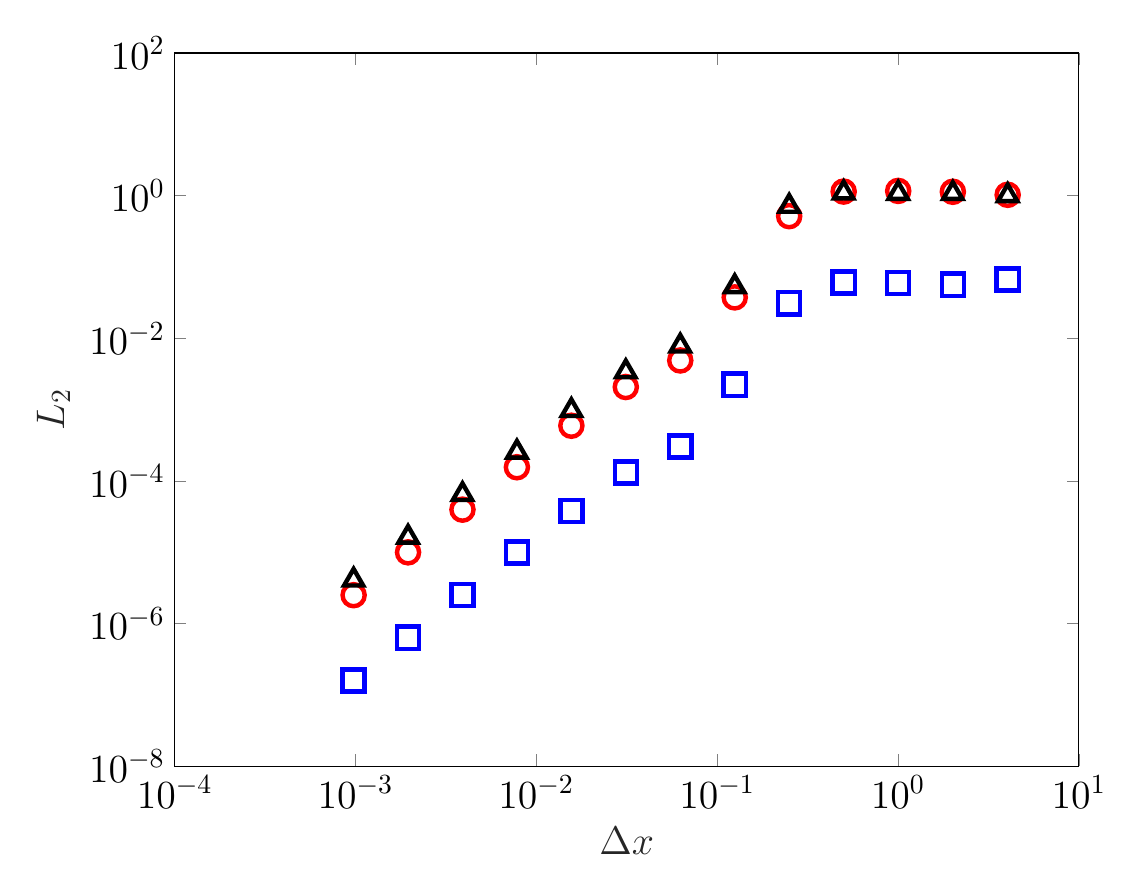
\begin{tikzpicture}
\tikzstyle{every node}=[font=\Large]

\begin{axis}[%
width=4.521in,
height=3.566in,
at={(0.758in,0.481in)},
every axis plot/.append style={ultra thick},
scale only axis,
xmode=log,
xmin=0.0001,
xmax=10,
xtick={0.0001,  0.001,   0.01,    0.1,      1,     10},
xminorticks=false,
xlabel style={font=\color{white!15!black}},
xlabel={\Large $\Delta x$},
ymode=log,
ymin=1e-08,
ymax=100,
ytick={ 1e-08,  1e-06, 0.0001,   0.01,      1,    100},
yminorticks=false,
ylabel style={font=\color{white!15!black}},
ylabel={\Large $L_2$},
axis background/.style={fill=white}
]
 \logLogSlopeTriangle{0.5}{0.2}{0.1}{2}{black};

\addplot [color=blue, draw=none, mark=square, mark size=4pt, mark options={solid, blue}, forget plot]
  table[row sep=crcr]{%
4.04040404040404	0.0667977316044187\\
2.01005025125628	0.0565251008982736\\
1.00250626566416	0.0600244047801842\\
0.500625782227785	0.060369043216863\\
0.250156347717323	0.031027562703989\\
0.125039074710847	0.00223720174663375\\
0.0625097671511174	0.000303213411708855\\
0.0312524415969998	0.00013195585438531\\
0.0156256103754053	3.78678120338089e-05\\
0.00781265259087092	9.90901359842452e-06\\
0.00390628814734519	2.52150220729934e-06\\
0.00195313453678973	6.35217079986901e-07\\
0.000976564884191612	1.59353271500116e-07\\
};
\addplot [color=red, draw=none, mark=o, mark size=4pt, mark options={solid, red}, forget plot]
  table[row sep=crcr]{%
4.04040404040404	1.02894168607817\\
2.01005025125628	1.13471870525711\\
1.00250626566416	1.16651134393852\\
0.500625782227785	1.14209935315627\\
0.250156347717323	0.516295949213657\\
0.125039074710847	0.0375055631709394\\
0.0625097671511174	0.0048956232734942\\
0.0312524415969998	0.00207713643544563\\
0.0156256103754053	0.000595469107815693\\
0.00781265259087092	0.00015580109802979\\
0.00390628814734519	3.96453330936357e-05\\
0.00195313453678973	9.98742874615667e-06\\
0.000976564884191612	2.5054904543415e-06\\
};
\addplot [color=black, draw=none, mark=triangle, mark size=4pt, mark options={solid, black}, forget plot]
  table[row sep=crcr]{%
4.04040404040404	1.00510027333734\\
2.01005025125628	1.07752750295002\\
1.00250626566416	1.07983904140976\\
0.500625782227785	1.09869881739817\\
0.250156347717323	0.712184449316794\\
0.125039074710847	0.05307095900171\\
0.0625097671511174	0.00781225049904385\\
0.0312524415969998	0.00340272133918679\\
0.0156256103754053	0.00097359240010264\\
0.00781265259087092	0.000254452413381455\\
0.00390628814734519	6.47146749585668e-05\\
0.00195313453678973	1.62988208772404e-05\\
0.000976564884191612	4.08829473005837e-06\\
};
%\addplot [color=mycolor1, forget plot]
%  table[row sep=crcr]{%
%4.04040404040404	16.3248648097133\\
%2.01005025125628	4.04030201257544\\
%1.00250626566416	1.0050188126959\\
%0.500625782227785	0.250626173831181\\
%0.250156347717323	0.0625781983032704\\
%0.125039074710847	0.0156347702045448\\
%0.0625097671511174	0.00390747098928691\\
%0.0312524415969998	0.000976715105773881\\
%0.0156256103754053	0.000244159699603973\\
%0.00781265259087092	6.1037540505642e-05\\
%0.00390628814734519	1.52590870900895e-05\\
%0.00195313453678973	3.81473451880083e-06\\
%0.000976564884191612	9.53678973036176e-07\\
%};
\end{axis}
\end{tikzpicture}%
\end{document}
	\caption{$L_2$ comparing numerical solution and forced soluiton}
\end{figure}


\subsection{Analytic Solution}
\subsubsection{Solitary Travelling Wave - Serre ($\beta_1=\beta_2 =0$) }
When $\beta_1 = \beta_2 = 0$ the gSGN are equivalent to the SGN equations which admit the following travelling wave solution

\begin{subequations}
	\begin{equation}
	h(x,t) = a_0 + a_1 \text{sech}^2\left( \kappa (x - ct) \right)
	\end{equation}
	\begin{equation}
	u(x,t) = c \left( 1- \dfrac{a_0}{h(x,t)} \right)
	\end{equation}
	where
	\begin{equation}
	\kappa = \dfrac{\sqrt{3a_1}}{2a_0 \sqrt{a_0 + a_1}}
	\end{equation}
	\begin{equation}
	c = \sqrt{g\left(a_0 + a_1\right)}
	\end{equation}
\end{subequations}

\begin{figure}
	\tikzset{every picture/.style={scale=0.9}}%
	\centering
	\begin{subfigure}{0.49\textwidth}
	\centering
	% This file was created by matlab2tikz.
%
%The latest updates can be retrieved from
%  http://www.mathworks.com/matlabcentral/fileexchange/22022-matlab2tikz-matlab2tikz
%where you can also make suggestions and rate matlab2tikz.
%
\begin{tikzpicture}

\begin{axis}[%
width=4.521in,
height=3.566in,
at={(0.758in,0.481in)},
scale only axis,
xmin=-50,
xmax=100,
xtick={-50,   0,  50, 100},
xlabel style={font=\color{white!15!black}},
xlabel={x (m)},
ymin=0.9,
ymax=1.6,
ytick={  1, 1.2, 1.4, 1.6},
ylabel style={font=\color{white!15!black}},
ylabel={h (m)},
axis background/.style={fill=white}
]
\addplot [color=blue, forget plot]
  table[row sep=crcr]{%
-50.2813379180994	1\\
-50.0468896530166	1\\
-49.8124413879337	1\\
-49.5779931228509	1\\
-49.3435448577681	1\\
-49.1090965926852	1\\
-48.8746483276024	1\\
-48.6402000625195	1\\
-48.4057517974367	1\\
-48.1713035323539	1\\
-47.936855267271	1\\
-47.7024070021882	1\\
-47.4679587371053	1\\
-47.2335104720225	1\\
-46.9990622069397	1\\
-46.7646139418568	1\\
-46.530165676774	1\\
-46.2957174116912	1\\
-46.0612691466083	1\\
-45.8268208815255	1\\
-45.5923726164426	1\\
-45.3579243513598	1\\
-45.123476086277	1\\
-44.8890278211941	1\\
-44.6545795561113	1\\
-44.4201312910284	1\\
-44.1856830259456	1\\
-43.9512347608628	1\\
-43.7167864957799	1\\
-43.4823382306971	1\\
-43.2478899656143	1\\
-43.0134417005314	1\\
-42.7789934354486	1\\
-42.5445451703657	1\\
-42.3100969052829	1\\
-42.0756486402001	1\\
-41.8412003751172	1\\
-41.6067521100344	1\\
-41.3723038449515	1\\
-41.1378555798687	1\\
-40.9034073147859	1\\
-40.668959049703	1\\
-40.4345107846202	1\\
-40.2000625195374	1\\
-39.9656142544545	1\\
-39.7311659893717	1\\
-39.4967177242888	1\\
-39.262269459206	1\\
-39.0278211941232	1\\
-38.7933729290403	1\\
-38.5589246639575	1\\
-38.3244763988747	1\\
-38.0900281337918	1\\
-37.855579868709	1\\
-37.6211316036261	1\\
-37.3866833385433	1\\
-37.1522350734605	1\\
-36.9177868083776	1\\
-36.6833385432948	1\\
-36.4488902782119	1\\
-36.2144420131291	1\\
-35.9799937480463	1\\
-35.7455454829634	1.00000000000001\\
-35.5110972178806	1.00000000000001\\
-35.2766489527977	1.00000000000002\\
-35.0422006877149	1.00000000000002\\
-34.8077524226321	1.00000000000004\\
-34.5733041575492	1.00000000000005\\
-34.3388558924664	1.00000000000008\\
-34.1044076273836	1.00000000000012\\
-33.8699593623007	1.00000000000018\\
-33.6355110972179	1.00000000000026\\
-33.401062832135	1.00000000000039\\
-33.1666145670522	1.00000000000057\\
-32.9321663019694	1.00000000000084\\
-32.6977180368865	1.00000000000123\\
-32.4632697718037	1.00000000000181\\
-32.2288215067208	1.00000000000264\\
-31.994373241638	1.00000000000385\\
-31.7599249765552	1.00000000000559\\
-31.5254767114723	1.0000000000081\\
-31.2910284463895	1.0000000000117\\
-31.0565801813067	1.00000000001686\\
-30.8221319162238	1.00000000002423\\
-30.587683651141	1.00000000003473\\
-30.3532353860581	1.00000000004965\\
-30.1187871209753	1.00000000007076\\
-29.8843388558925	1.00000000010059\\
-29.6498905908096	1.00000000014259\\
-29.4154423257268	1.00000000020158\\
-29.180994060644	1.00000000028418\\
-28.9465457955611	1.00000000039954\\
-28.7120975304783	1.00000000056018\\
-28.4776492653954	1.00000000078326\\
-28.2432010003126	1.00000000109216\\
-28.0087527352298	1.00000000151871\\
-27.7743044701469	1.00000000210606\\
-27.5398562050641	1.00000000291254\\
-27.3054079399812	1.0000000040168\\
-27.0709596748984	1.00000000552452\\
-26.8365114098156	1.00000000757732\\
-26.6020631447327	1.00000001036438\\
-26.3676148796499	1.00000001413764\\
-26.1331666145671	1.00000001923168\\
-25.8987183494842	1.00000002608938\\
-25.6642700844014	1.0000000352953\\
-25.4298218193185	1.00000004761857\\
-25.1953735542357	1.00000006406816\\
-24.9609252891529	1.00000008596359\\
-24.72647702407	1.00000011502529\\
-24.4920287589872	1.00000015348945\\
-24.2575804939043	1.00000020425381\\
-24.0231322288215	1.00000027106174\\
-23.7886839637387	1.00000035873413\\
-23.5542356986558	1.00000047346035\\
-23.319787433573	1.00000062316199\\
-23.0853391684902	1.00000081794618\\
-22.8508909034073	1.00000107066827\\
-22.6164426383245	1.00000139762789\\
-22.3819943732416	1.00000181942692\\
-22.1475461081588	1.0000023620229\\
-21.913097843076	1.00000305801787\\
-21.6786495779931	1.00000394822926\\
-21.4442013129103	1.00000508359724\\
-21.2097530478274	1.00000652749182\\
-20.9753047827446	1.00000835849268\\
-20.7408565176618	1.00001067372539\\
-20.5064082525789	1.00001359284963\\
-20.2719599874961	1.00001726280754\\
-20.0375117224133	1.00002186345402\\
-19.8030634573304	1.00002761420516\\
-19.5686151922476	1.00003478185573\\
-19.3341669271647	1.00004368973197\\
-19.0997186620819	1.00005472836075\\
-18.8652703969991	1.00006836785094\\
-18.6308221319162	1.00008517219618\\
-18.3963738668334	1.00010581572006\\
-18.1619256017505	1.00013110189409\\
-17.9274773366677	1.00016198476474\\
-17.6930290715849	1.00019959322775\\
-17.458580806502	1.0002452583839\\
-17.2241325414192	1.00030054420029\\
-16.9896842763364	1.00036728168296\\
-16.7552360112535	1.00044760673918\\
-16.5207877461707	1.00054400186957\\
-16.2863394810878	1.00065934178048\\
-16.051891216005	1.0007969429435\\
-15.8174429509222	1.00096061705131\\
-15.5829946858393	1.0011547282258\\
-15.3485464207565	1.00138425372495\\
-15.1140981556737	1.0016548477687\\
-14.8796498905908	1.00197290796114\\
-14.645201625508	1.0023456436272\\
-14.4107533604251	1.00278114520757\\
-14.1763050953423	1.00328845366785\\
-13.9418568302595	1.00387762867878\\
-13.7074085651766	1.00455981411803\\
-13.4729603000938	1.00534729923322\\
-13.2385120350109	1.00625357359717\\
-13.0040637699281	1.00729337378393\\
-12.7696155048453	1.00848271950624\\
-12.5351672397624	1.00983893678776\\
-12.3007189746796	1.01138066560577\\
-12.0662707095968	1.01312784934003\\
-11.8318224445139	1.01510170331021\\
-11.5973741794311	1.01732465968668\\
-11.3629259143482	1.01982028612648\\
-11.1284776492654	1.02261317562514\\
-10.8940293841826	1.02572880529488\\
-10.6595811190997	1.02919336208441\\
-10.4251328540169	1.03303353385146\\
-10.190684588934	1.03727626468739\\
-9.95623632385121	1.04194847397484\\
-9.72178805876837	1.04707673933045\\
-9.48733979368553	1.05268694434153\\
-9.25289152860269	1.05880389283676\\
-9.01844326351986	1.06545089232737\\
-8.78399499843702	1.07264931019819\\
-8.54954673335418	1.0804181072015\\
-8.31509846827134	1.08877335378647\\
-8.0806502031885	1.09772773576034\\
-7.84620193810566	1.10729005669583\\
-7.61175367302283	1.11746474534576\\
-7.37730540793999	1.12825137706879\\
-7.14285714285715	1.13964421888189\\
-6.90840887777431	1.15163180820559\\
-6.67396061269147	1.16419657562992\\
-6.43951234760863	1.17731452207938\\
-6.20506408252579	1.19095496057201\\
-5.97061581744295	1.20508033233635\\
-5.73616755236011	1.21964610636083\\
-5.50171928727728	1.23460077049871\\
-5.26727102219444	1.24988592104312\\
-5.0328227571116	1.26543645623178\\
-4.79837449202876	1.28118087745916\\
-4.56392622694592	1.29704170009199\\
-4.32947796186308	1.3129359737373\\
-4.09502969678024	1.32877590964158\\
-3.86058143169741	1.34446961065261\\
-3.62613316661457	1.35992189690531\\
-3.39168490153173	1.37503521815484\\
-3.15723663644889	1.38971064153283\\
-2.92278837136605	1.40384890150489\\
-2.68834010628321	1.41735149701592\\
-2.45389184120038	1.43012181927902\\
-2.21944357611754	1.44206629244249\\
-1.9849953110347	1.45309550850012\\
-1.75054704595186	1.46312533732628\\
-1.51609878086902	1.47207799264432\\
-1.28165051578619	1.47988303508748\\
-1.04720225070335	1.486478294289\\
-0.81275398562051	1.49181069313261\\
-0.578305720537671	1.49583695888505\\
-0.343857455454831	1.4985242078866\\
-0.109409190371991	1.49985039275007\\
0.125039074710841	1.49980460356216\\
0.359487339793681	1.49838721733138\\
0.593935604876521	1.49560989281925\\
0.82838386995936	1.49149541085385\\
1.0628321350422	1.48607736318493\\
1.29728040012503	1.47939969582472\\
1.53172866520787	1.47151611555753\\
1.76617693029071	1.46248937082802\\
2.00062519537355	1.45239042047313\\
2.23507346045639	1.44129750569374\\
2.46952172553923	1.42929514222706\\
2.70396999062206	1.41647305084817\\
2.9384182557049	1.40292504507801\\
3.17286652078774	1.38874789529779\\
3.40731478587058	1.37404018836833\\
3.64176305095342	1.3589012013431\\
3.87621131603625	1.34342980696942\\
4.11065958111909	1.32772342742918\\
4.34510784620193	1.31187705122056\\
4.57955611128477	1.2959823262753\\
4.81400437636761	1.28012674039652\\
5.04845264145045	1.26439289794664\\
5.28290090653329	1.2488578994733\\
5.51734917161613	1.23359282869048\\
5.75179743669896	1.21866234898853\\
5.9862457017818	1.20412440948336\\
6.22069396686464	1.19003005857757\\
6.45514223194748	1.1764233611373\\
6.68959049703032	1.16334141372086\\
6.92403876211316	1.15081445085613\\
7.158487027196	1.13886603417211\\
7.39293529227884	1.12751331525607\\
7.62738355736168	1.11676736243566\\
7.86183182244451	1.10663354127118\\
8.09628008752735	1.09711193837608\\
8.33072835261019	1.08819781824871\\
8.56517661769303	1.07988210307379\\
8.79962488277587	1.07215186591426\\
9.0340731478587	1.06499082833496\\
9.26852141294154	1.05837985425115\\
9.50296967802438	1.05229743264634\\
9.73741794310722	1.04672014272671\\
9.97186620819006	1.04162309604406\\
10.2063144732729	1.03698035110013\\
10.4407627383557	1.03276529691662\\
10.6752110034386	1.02895100299605\\
10.9096592685214	1.0255105339908\\
11.1441075336042	1.02241722822454\\
11.3785557986871	1.01964493996135\\
11.6130040637699	1.01716824598324\\
11.8474523288528	1.0149626176121\\
12.0819005939356	1.01300455979442\\
12.3163488590184	1.0112717192563\\
12.5507971241013	1.00974296403593\\
12.7852453891841	1.00839843691411\\
13.019693654267	1.00721958539794\\
13.2541419193498	1.00618917097478\\
13.4885901844326	1.00529126035223\\
13.7230384495155	1.00451120134316\\
13.9574867145983	1.00383558595183\\
14.1919349796812	1.00325220307764\\
14.426383244764	1.00274998308377\\
14.6608315098468	1.00231893628901\\
14.8952797749297	1.00195008723815\\
15.1297280400125	1.00163540639697\\
15.3641763050953	1.00136774070769\\
15.5986245701782	1.00114074423417\\
15.833072835261	1.00094880992829\\
16.0675211003439	1.00078700336147\\
16.3019693654267	1.00065099909212\\
16.5364176305095	1.00053702018171\\
16.7708658955924	1.00044178123018\\
17.0053141606752	1.00036243517649\\
17.239762425758	1.00029652400162\\
17.4742106908409	1.0002419333792\\
17.7086589559237	1.00019685124205\\
17.9431072210066	1.00015973017075\\
18.1775554860894	1.00012925346107\\
18.4120037511722	1.00010430468965\\
18.6464520162551	1.00008394057076\\
18.8809002813379	1.00006736687926\\
19.1153485464207	1.00005391720483\\
19.3497968115036	1.00004303429953\\
19.5842450765864	1.00003425378251\\
19.8186933416693	1.00002718997212\\
20.0531416067521	1.00002152362502\\
20.2875898718349	1.00001699137406\\
20.5220381369178	1.00001337667\\
20.7564864020006	1.00001050204693\\
20.9909346670835	1.00000822254624\\
21.2253829321663	1.00000642014923\\
21.4598311972491	1.00000499908303\\
21.694279462332	1.00000388187911\\
21.9287277274148	1.00000300607693\\
22.1631759924977	1.00000232147817\\
22.3976242575805	1.00000178786839\\
22.6320725226633	1.00000137313399\\
22.8665207877462	1.00000105171173\\
23.100969052829	1.00000080331698\\
23.3354173179118	1.00000061190444\\
23.5698655829947	1.00000046482201\\
23.8043138480775	1.00000035212447\\
24.0387621131604	1.00000026601869\\
24.2732103782432	1.00000020041698\\
24.507658643326	1.00000015057862\\
24.7421069084089	1.00000011282323\\
24.9765551734917	1.00000008430245\\
25.2110034385746	1.00000006281861\\
25.4454517036574	1.00000004668129\\
25.6798999687402	1.00000003459424\\
25.9143482338231	1.00000002556649\\
26.1487964989059	1.00000001884278\\
26.3832447639887	1.00000001384921\\
26.6176930290716	1.00000001015107\\
26.8521412941544	1.00000000742002\\
27.0865895592373	1.00000000540884\\
27.3210378243201	1.00000000393197\\
27.5554860894029	1.00000000285051\\
27.7899343544858	1.00000000206083\\
28.0243826195686	1.00000000148582\\
28.2588308846514	1.00000000106831\\
28.4932791497343	1.00000000076601\\
28.7277274148171	1.00000000054775\\
28.9621756799	1.0000000003906\\
29.1966239449828	1.00000000027777\\
29.4310722100656	1.00000000019699\\
29.6655204751485	1.00000000013932\\
29.8999687402313	1.00000000009827\\
30.1344170053141	1.00000000006912\\
30.368865270397	1.00000000004848\\
30.6033135354798	1.00000000003391\\
30.8377618005627	1.00000000002366\\
31.0722100656455	1.00000000001646\\
31.3066583307284	1.00000000001142\\
31.5411065958112	1.0000000000079\\
31.775554860894	1.00000000000545\\
32.0100031259769	1.00000000000375\\
32.2444513910597	1.00000000000257\\
32.4788996561425	1.00000000000176\\
32.7133479212254	1.0000000000012\\
32.9477961863082	1.00000000000082\\
33.1822444513911	1.00000000000056\\
33.4166927164739	1.00000000000038\\
33.6511409815567	1.00000000000025\\
33.8855892466396	1.00000000000017\\
34.1200375117224	1.00000000000011\\
34.3544857768052	1.00000000000008\\
34.5889340418881	1.00000000000005\\
34.8233823069709	1.00000000000003\\
35.0578305720538	1.00000000000002\\
35.2922788371366	1.00000000000001\\
35.5267271022194	1.00000000000001\\
35.7611753673023	1.00000000000001\\
35.9956236323851	1\\
36.230071897468	1\\
36.4645201625508	1\\
36.6989684276336	1\\
36.9334166927165	1\\
37.1678649577993	1\\
37.4023132228821	1\\
37.636761487965	1\\
37.8712097530478	1\\
38.1056580181307	1\\
38.3401062832135	1\\
38.5745545482963	1\\
38.8090028133792	1\\
39.043451078462	1\\
39.2778993435448	1\\
39.5123476086277	1\\
39.7467958737105	1\\
39.9812441387934	1\\
40.2156924038762	1\\
40.450140668959	1\\
40.6845889340419	1\\
40.9190371991247	1\\
41.1534854642076	1\\
41.3879337292904	1\\
41.6223819943732	1\\
41.8568302594561	1\\
42.0912785245389	1\\
42.3257267896218	1\\
42.5601750547046	1\\
42.7946233197874	1\\
43.0290715848703	1\\
43.2635198499531	1\\
43.4979681150359	1\\
43.7324163801188	1\\
43.9668646452016	1\\
44.2013129102845	1\\
44.4357611753673	1\\
44.6702094404501	1\\
44.904657705533	1\\
45.1391059706158	1\\
45.3735542356986	1\\
45.6080025007815	1\\
45.8424507658643	1\\
46.0768990309472	1\\
46.31134729603	1\\
46.5457955611128	1\\
46.7802438261957	1\\
47.0146920912785	1\\
47.2491403563614	1\\
47.4835886214442	1\\
47.718036886527	1\\
47.9524851516099	1\\
48.1869334166927	1\\
48.4213816817755	1\\
48.6558299468584	1\\
48.8902782119412	1\\
49.1247264770241	1\\
49.3591747421069	1\\
49.5936230071897	1\\
49.8280712722726	1\\
50.0625195373554	1\\
50.2969678024383	1\\
50.5314160675211	1\\
50.7658643326039	1\\
51.0003125976868	1\\
51.2347608627696	1\\
51.4692091278525	1\\
51.7036573929353	1\\
51.9381056580181	1\\
52.172553923101	1\\
52.4070021881838	1\\
52.6414504532666	1\\
52.8758987183495	1\\
53.1103469834323	1\\
53.3447952485152	1\\
53.579243513598	1\\
53.8136917786808	1\\
54.0481400437637	1\\
54.2825883088465	1\\
54.5170365739293	1\\
54.7514848390122	1\\
54.985933104095	1\\
55.2203813691779	1\\
55.4548296342607	1\\
55.6892778993435	1\\
55.9237261644264	1\\
56.1581744295092	1\\
56.392622694592	1\\
56.6270709596749	1\\
56.8615192247577	1\\
57.0959674898406	1\\
57.3304157549234	1\\
57.5648640200062	1\\
57.7993122850891	1\\
58.0337605501719	1\\
58.2682088152548	1\\
58.5026570803376	1\\
58.7371053454204	1\\
58.9715536105033	1\\
59.2060018755861	1\\
59.440450140669	1\\
59.6748984057518	1\\
59.9093466708346	1\\
60.1437949359175	1\\
60.3782432010003	1\\
60.6126914660831	1\\
60.847139731166	1\\
61.0815879962488	1\\
61.3160362613317	1\\
61.5504845264145	1\\
61.7849327914973	1\\
62.0193810565802	1\\
62.253829321663	1\\
62.4882775867459	1\\
62.7227258518287	1\\
62.9571741169115	1\\
63.1916223819944	1\\
63.4260706470772	1\\
63.66051891216	1\\
63.8949671772429	1\\
64.1294154423257	1\\
64.3638637074086	1\\
64.5983119724914	1\\
64.8327602375742	1\\
65.0672085026571	1\\
65.3016567677399	1\\
65.5361050328227	1\\
65.7705532979056	1\\
66.0050015629884	1\\
66.2394498280713	1\\
66.4738980931541	1\\
66.7083463582369	1\\
66.9427946233198	1\\
67.1772428884026	1\\
67.4116911534854	1\\
67.6461394185683	1\\
67.8805876836511	1\\
68.115035948734	1\\
68.3494842138168	1\\
68.5839324788997	1\\
68.8183807439825	1\\
69.0528290090653	1\\
69.2872772741482	1\\
69.521725539231	1\\
69.7561738043138	1\\
69.9906220693967	1\\
70.2250703344795	1\\
70.4595185995624	1\\
70.6939668646452	1\\
70.928415129728	1\\
71.1628633948109	1\\
71.3973116598937	1\\
71.6317599249765	1\\
71.8662081900594	1\\
72.1006564551422	1\\
72.3351047202251	1\\
72.5695529853079	1\\
72.8040012503907	1\\
73.0384495154736	1\\
73.2728977805564	1\\
73.5073460456393	1\\
73.7417943107221	1\\
73.9762425758049	1\\
74.2106908408878	1\\
74.4451391059706	1\\
74.6795873710534	1\\
74.9140356361363	1\\
75.1484839012191	1\\
75.382932166302	1\\
75.6173804313848	1\\
75.8518286964676	1\\
76.0862769615505	1\\
76.3207252266333	1\\
76.5551734917161	1\\
76.789621756799	1\\
77.0240700218818	1\\
77.2585182869647	1\\
77.4929665520475	1\\
77.7274148171303	1\\
77.9618630822132	1\\
78.196311347296	1\\
78.4307596123789	1\\
78.6652078774617	1\\
78.8996561425445	1\\
79.1341044076274	1\\
79.3685526727102	1\\
79.603000937793	1\\
79.8374492028759	1\\
80.0718974679587	1\\
80.3063457330416	1\\
80.5407939981244	1\\
80.7752422632072	1\\
81.0096905282901	1\\
81.2441387933729	1\\
81.4785870584558	1\\
81.7130353235386	1\\
81.9474835886214	1\\
82.1819318537043	1\\
82.4163801187871	1\\
82.65082838387	1\\
82.8852766489528	1\\
83.1197249140356	1\\
83.3541731791185	1\\
83.5886214442013	1\\
83.8230697092841	1\\
84.057517974367	1\\
84.2919662394498	1\\
84.5264145045327	1\\
84.7608627696155	1\\
84.9953110346983	1\\
85.2297592997812	1\\
85.464207564864	1\\
85.6986558299469	1\\
85.9331040950297	1\\
86.1675523601125	1\\
86.4020006251954	1\\
86.6364488902782	1\\
86.870897155361	1\\
87.1053454204439	1\\
87.3397936855267	1\\
87.5742419506095	1\\
87.8086902156924	1\\
88.0431384807752	1\\
88.2775867458581	1\\
88.5120350109409	1\\
88.7464832760238	1\\
88.9809315411066	1\\
89.2153798061894	1\\
89.4498280712723	1\\
89.6842763363551	1\\
89.9187246014379	1\\
90.1531728665208	1\\
90.3876211316036	1\\
90.6220693966864	1\\
90.8565176617693	1\\
91.0909659268521	1\\
91.325414191935	1\\
91.5598624570178	1\\
91.7943107221006	1\\
92.0287589871835	1\\
92.2632072522663	1\\
92.4976555173492	1\\
92.732103782432	1\\
92.9665520475149	1\\
93.2010003125977	1\\
93.4354485776805	1\\
93.6698968427634	1\\
93.9043451078462	1\\
94.138793372929	1\\
94.3732416380119	1\\
94.6076899030947	1\\
94.8421381681775	1\\
95.0765864332604	1\\
95.3110346983432	1\\
95.5454829634261	1\\
95.7799312285089	1\\
96.0143794935917	1\\
96.2488277586746	1\\
96.4832760237574	1\\
96.7177242888403	1\\
96.9521725539231	1\\
97.1866208190059	1\\
97.4210690840888	1\\
97.6555173491716	1\\
97.8899656142544	1\\
98.1244138793373	1\\
98.3588621444201	1\\
98.5933104095029	1\\
98.8277586745858	1\\
99.0622069396686	1\\
99.2966552047515	1\\
99.5311034698343	1\\
99.7655517349172	1\\
100	1\\
100.234448265083	1\\
};
\end{axis}
\end{tikzpicture}%
	\caption{$t = 0s$}
	\end{subfigure}
	\begin{subfigure}{0.49\textwidth}
	\centering
	% This file was created by matlab2tikz.
%
%The latest updates can be retrieved from
%  http://www.mathworks.com/matlabcentral/fileexchange/22022-matlab2tikz-matlab2tikz
%where you can also make suggestions and rate matlab2tikz.
%
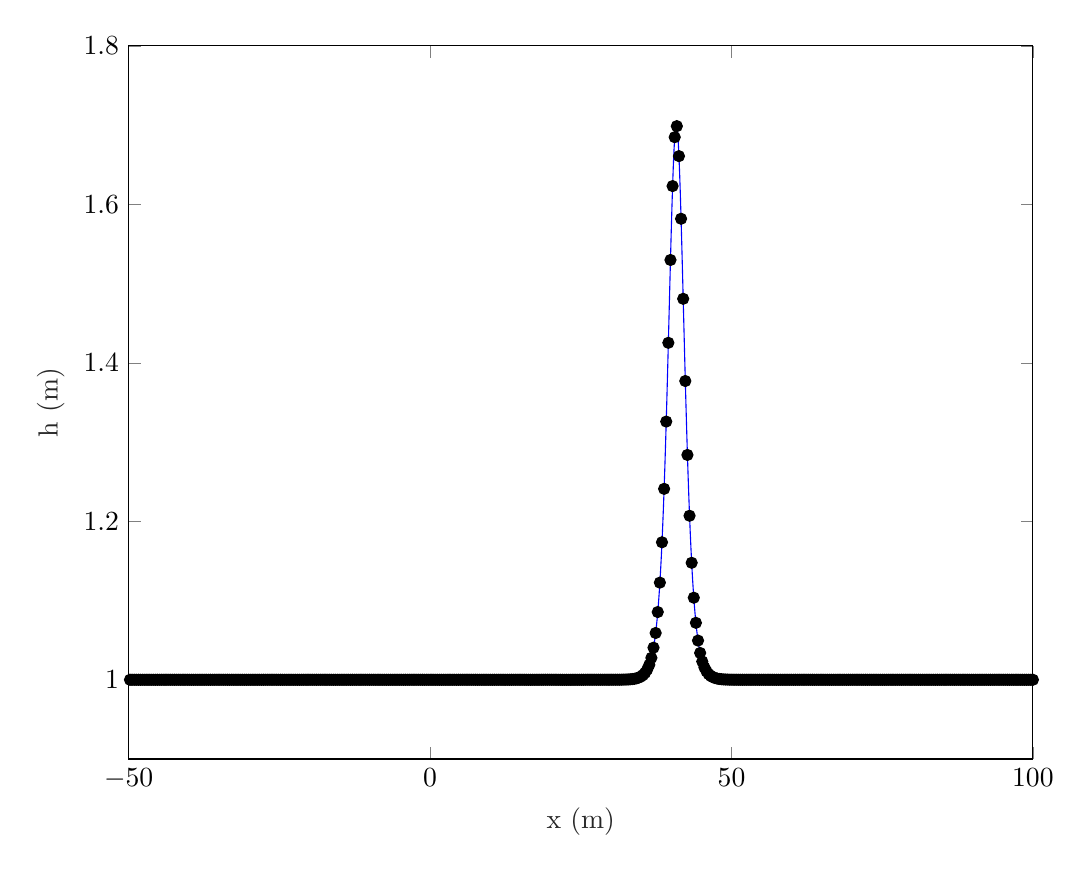
\begin{tikzpicture}

\begin{axis}[%
width=4.521in,
height=3.566in,
at={(0.758in,0.481in)},
scale only axis,
xmin=-50,
xmax=100,
xtick={-50,   0,  50, 100},
xlabel style={font=\color{white!15!black}},
xlabel={x (m)},
ymin=0.9,
ymax=1.8,
ytick={  1, 1.2, 1.4, 1.6, 1.8},
ylabel style={font=\color{white!15!black}},
ylabel={h (m)},
axis background/.style={fill=white}
]
\addplot [color=blue, forget plot]
  table[row sep=crcr]{%
-50.14064697609	1\\
-50.0234411626817	1\\
-49.9062353492733	1\\
-49.789029535865	1\\
-49.6718237224566	1\\
-49.5546179090483	1\\
-49.4374120956399	1\\
-49.3202062822316	1\\
-49.2030004688233	1\\
-49.0857946554149	1\\
-48.9685888420066	1\\
-48.8513830285982	1\\
-48.7341772151899	1\\
-48.6169714017815	1\\
-48.4997655883732	1\\
-48.3825597749648	1\\
-48.2653539615565	1\\
-48.1481481481481	1\\
-48.0309423347398	1\\
-47.9137365213315	1\\
-47.7965307079231	1\\
-47.6793248945148	1\\
-47.5621190811064	1\\
-47.4449132676981	1\\
-47.3277074542897	1\\
-47.2105016408814	1\\
-47.093295827473	1\\
-46.9760900140647	1\\
-46.8588842006564	1\\
-46.741678387248	1\\
-46.6244725738397	1\\
-46.5072667604313	1\\
-46.390060947023	1\\
-46.2728551336146	1\\
-46.1556493202063	1\\
-46.0384435067979	1\\
-45.9212376933896	1\\
-45.8040318799812	1\\
-45.6868260665729	1\\
-45.5696202531646	1\\
-45.4524144397562	1\\
-45.3352086263479	1\\
-45.2180028129395	1\\
-45.1007969995312	1\\
-44.9835911861228	1\\
-44.8663853727145	1\\
-44.7491795593061	1\\
-44.6319737458978	1\\
-44.5147679324894	1\\
-44.3975621190811	1\\
-44.2803563056728	1\\
-44.1631504922644	1\\
-44.0459446788561	1\\
-43.9287388654477	1\\
-43.8115330520394	1\\
-43.694327238631	1\\
-43.5771214252227	1\\
-43.4599156118143	1\\
-43.342709798406	1\\
-43.2255039849977	1\\
-43.1082981715893	1\\
-42.991092358181	1\\
-42.8738865447726	1\\
-42.7566807313643	1\\
-42.6394749179559	1\\
-42.5222691045476	1\\
-42.4050632911392	1\\
-42.2878574777309	1\\
-42.1706516643225	1\\
-42.0534458509142	1\\
-41.9362400375059	1\\
-41.8190342240975	1\\
-41.7018284106892	1\\
-41.5846225972808	1\\
-41.4674167838725	1\\
-41.3502109704641	1\\
-41.2330051570558	1\\
-41.1157993436474	1\\
-40.9985935302391	1\\
-40.8813877168308	1\\
-40.7641819034224	1\\
-40.6469760900141	1\\
-40.5297702766057	1\\
-40.4125644631974	1\\
-40.295358649789	1\\
-40.1781528363807	1\\
-40.0609470229723	1\\
-39.943741209564	1\\
-39.8265353961556	1\\
-39.7093295827473	1\\
-39.592123769339	1\\
-39.4749179559306	1\\
-39.3577121425223	1\\
-39.2405063291139	1\\
-39.1233005157056	1\\
-39.0060947022972	1\\
-38.8888888888889	1\\
-38.7716830754805	1\\
-38.6544772620722	1\\
-38.5372714486639	1\\
-38.4200656352555	1\\
-38.3028598218472	1\\
-38.1856540084388	1\\
-38.0684481950305	1\\
-37.9512423816221	1\\
-37.8340365682138	1\\
-37.7168307548054	1\\
-37.5996249413971	1\\
-37.4824191279887	1\\
-37.3652133145804	1\\
-37.2480075011721	1\\
-37.1308016877637	1\\
-37.0135958743554	1\\
-36.896390060947	1\\
-36.7791842475387	1\\
-36.6619784341303	1\\
-36.544772620722	1\\
-36.4275668073136	1\\
-36.3103609939053	1\\
-36.193155180497	1\\
-36.0759493670886	1\\
-35.9587435536803	1\\
-35.8415377402719	1\\
-35.7243319268636	1\\
-35.6071261134552	1\\
-35.4899203000469	1\\
-35.3727144866385	1\\
-35.2555086732302	1\\
-35.1383028598218	1\\
-35.0210970464135	1\\
-34.9038912330052	1\\
-34.7866854195968	1\\
-34.6694796061885	1\\
-34.5522737927801	1\\
-34.4350679793718	1\\
-34.3178621659634	1\\
-34.2006563525551	1\\
-34.0834505391467	1\\
-33.9662447257384	1\\
-33.8490389123301	1\\
-33.7318330989217	1\\
-33.6146272855134	1\\
-33.497421472105	1\\
-33.3802156586967	1\\
-33.2630098452883	1\\
-33.14580403188	1\\
-33.0285982184716	1\\
-32.9113924050633	1\\
-32.7941865916549	1\\
-32.6769807782466	1\\
-32.5597749648383	1\\
-32.4425691514299	1\\
-32.3253633380216	1\\
-32.2081575246132	1\\
-32.0909517112049	1\\
-31.9737458977965	1\\
-31.8565400843882	1\\
-31.7393342709798	1\\
-31.6221284575715	1\\
-31.5049226441632	1\\
-31.3877168307548	1\\
-31.2705110173465	1\\
-31.1533052039381	1\\
-31.0360993905298	1\\
-30.9188935771214	1\\
-30.8016877637131	1\\
-30.6844819503047	1\\
-30.5672761368964	1\\
-30.450070323488	1\\
-30.3328645100797	1\\
-30.2156586966714	1\\
-30.098452883263	1\\
-29.9812470698547	1\\
-29.8640412564463	1\\
-29.746835443038	1\\
-29.6296296296296	1\\
-29.5124238162213	1\\
-29.3952180028129	1\\
-29.2780121894046	1\\
-29.1608063759962	1\\
-29.0436005625879	1\\
-28.9263947491796	1\\
-28.8091889357712	1\\
-28.6919831223629	1\\
-28.5747773089545	1\\
-28.4575714955462	1\\
-28.3403656821378	1\\
-28.2231598687295	1\\
-28.1059540553211	1\\
-27.9887482419128	1\\
-27.8715424285045	1\\
-27.7543366150961	1\\
-27.6371308016878	1\\
-27.5199249882794	1\\
-27.4027191748711	1\\
-27.2855133614627	1\\
-27.1683075480544	1\\
-27.051101734646	1\\
-26.9338959212377	1\\
-26.8166901078293	1\\
-26.699484294421	1\\
-26.5822784810127	1\\
-26.4650726676043	1\\
-26.347866854196	1\\
-26.2306610407876	1\\
-26.1134552273793	1\\
-25.9962494139709	1\\
-25.8790436005626	1\\
-25.7618377871542	1\\
-25.6446319737459	1\\
-25.5274261603376	1\\
-25.4102203469292	1\\
-25.2930145335209	1\\
-25.1758087201125	1\\
-25.0586029067042	1\\
-24.9413970932958	1\\
-24.8241912798875	1\\
-24.7069854664791	1\\
-24.5897796530708	1\\
-24.4725738396624	1\\
-24.3553680262541	1\\
-24.2381622128458	1\\
-24.1209563994374	1\\
-24.0037505860291	1\\
-23.8865447726207	1\\
-23.7693389592124	1\\
-23.652133145804	1\\
-23.5349273323957	1\\
-23.4177215189873	1\\
-23.300515705579	1\\
-23.1833098921707	1\\
-23.0661040787623	1\\
-22.948898265354	1\\
-22.8316924519456	1\\
-22.7144866385373	1\\
-22.5972808251289	1\\
-22.4800750117206	1\\
-22.3628691983122	1\\
-22.2456633849039	1\\
-22.1284575714955	1\\
-22.0112517580872	1\\
-21.8940459446789	1\\
-21.7768401312705	1\\
-21.6596343178622	1\\
-21.5424285044538	1\\
-21.4252226910455	1\\
-21.3080168776371	1\\
-21.1908110642288	1\\
-21.0736052508204	1\\
-20.9563994374121	1\\
-20.8391936240038	1\\
-20.7219878105954	1\\
-20.6047819971871	1\\
-20.4875761837787	1\\
-20.3703703703704	1\\
-20.253164556962	1\\
-20.1359587435537	1\\
-20.0187529301453	1\\
-19.901547116737	1\\
-19.7843413033286	1\\
-19.6671354899203	1\\
-19.549929676512	1\\
-19.4327238631036	1\\
-19.3155180496953	1\\
-19.1983122362869	1\\
-19.0811064228786	1\\
-18.9639006094702	1\\
-18.8466947960619	1\\
-18.7294889826535	1\\
-18.6122831692452	1\\
-18.4950773558368	1\\
-18.3778715424285	1\\
-18.2606657290202	1\\
-18.1434599156118	1\\
-18.0262541022035	1\\
-17.9090482887951	1\\
-17.7918424753868	1\\
-17.6746366619784	1\\
-17.5574308485701	1\\
-17.4402250351617	1\\
-17.3230192217534	1\\
-17.2058134083451	1\\
-17.0886075949367	1\\
-16.9714017815284	1\\
-16.85419596812	1\\
-16.7369901547117	1\\
-16.6197843413033	1\\
-16.502578527895	1\\
-16.3853727144866	1\\
-16.2681669010783	1\\
-16.1509610876699	1\\
-16.0337552742616	1\\
-15.9165494608533	1\\
-15.7993436474449	1\\
-15.6821378340366	1\\
-15.5649320206282	1\\
-15.4477262072199	1\\
-15.3305203938115	1\\
-15.2133145804032	1\\
-15.0961087669948	1\\
-14.9789029535865	1\\
-14.8616971401782	1\\
-14.7444913267698	1\\
-14.6272855133615	1\\
-14.5100796999531	1\\
-14.3928738865448	1\\
-14.2756680731364	1\\
-14.1584622597281	1\\
-14.0412564463197	1\\
-13.9240506329114	1\\
-13.806844819503	1\\
-13.6896390060947	1\\
-13.5724331926864	1\\
-13.455227379278	1\\
-13.3380215658697	1\\
-13.2208157524613	1\\
-13.103609939053	1\\
-12.9864041256446	1\\
-12.8691983122363	1\\
-12.7519924988279	1\\
-12.6347866854196	1\\
-12.5175808720113	1\\
-12.4003750586029	1\\
-12.2831692451946	1\\
-12.1659634317862	1\\
-12.0487576183779	1\\
-11.9315518049695	1\\
-11.8143459915612	1\\
-11.6971401781528	1\\
-11.5799343647445	1\\
-11.4627285513361	1\\
-11.3455227379278	1\\
-11.2283169245195	1\\
-11.1111111111111	1\\
-10.9939052977028	1\\
-10.8766994842944	1\\
-10.7594936708861	1\\
-10.6422878574777	1\\
-10.5250820440694	1\\
-10.407876230661	1\\
-10.2906704172527	1\\
-10.1734646038444	1\\
-10.056258790436	1\\
-9.93905297702766	1\\
-9.82184716361932	1\\
-9.70464135021097	1\\
-9.58743553680262	1\\
-9.47022972339428	1\\
-9.35302390998594	1\\
-9.23581809657759	1\\
-9.11861228316924	1\\
-9.0014064697609	1\\
-8.88420065635255	1\\
-8.76699484294421	1\\
-8.64978902953587	1\\
-8.53258321612752	1\\
-8.41537740271917	1\\
-8.29817158931083	1\\
-8.18096577590249	1\\
-8.06375996249414	1\\
-7.94655414908579	1\\
-7.82934833567745	1\\
-7.7121425222691	1\\
-7.59493670886076	1\\
-7.47773089545242	1\\
-7.36052508204407	1\\
-7.24331926863572	1\\
-7.12611345522738	1\\
-7.00890764181904	1\\
-6.89170182841069	1\\
-6.77449601500234	1\\
-6.657290201594	1\\
-6.54008438818565	1\\
-6.42287857477731	1\\
-6.30567276136896	1\\
-6.18846694796062	1\\
-6.07126113455227	1\\
-5.95405532114393	1\\
-5.83684950773559	1\\
-5.71964369432724	1\\
-5.60243788091889	1\\
-5.48523206751055	1\\
-5.3680262541022	1\\
-5.25082044069386	1\\
-5.13361462728551	1\\
-5.01640881387717	1\\
-4.89920300046882	1\\
-4.78199718706048	1\\
-4.66479137365214	1\\
-4.54758556024379	1\\
-4.43037974683544	1\\
-4.31317393342709	1\\
-4.19596812001875	1\\
-4.07876230661041	1\\
-3.96155649320206	1\\
-3.84435067979372	1\\
-3.72714486638537	1\\
-3.60993905297703	1\\
-3.49273323956868	1\\
-3.37552742616034	1\\
-3.25832161275199	1\\
-3.14111579934364	1\\
-3.0239099859353	1\\
-2.90670417252696	1\\
-2.78949835911861	1\\
-2.67229254571027	1\\
-2.55508673230192	1\\
-2.43788091889358	1\\
-2.32067510548523	1\\
-2.20346929207689	1\\
-2.08626347866854	1\\
-1.96905766526019	1\\
-1.85185185185185	1\\
-1.73464603844351	1\\
-1.61744022503516	1\\
-1.50023441162681	1\\
-1.38302859821847	1\\
-1.26582278481013	1\\
-1.14861697140178	1\\
-1.03141115799344	1\\
-0.914205344585092	1\\
-0.796999531176745	1\\
-0.679793717768398	1\\
-0.562587904360058	1\\
-0.445382090951711	1\\
-0.328176277543363	1\\
-0.210970464135023	1\\
-0.0937646507266763	1\\
0.0234411626816708	1\\
0.140646976090011	1\\
0.257852789498358	1\\
0.375058602906705	1\\
0.492264416315052	1\\
0.609470229723392	1\\
0.726676043131739	1\\
0.843881856540087	1\\
0.961087669948427	1\\
1.07829348335677	1\\
1.19549929676512	1\\
1.31270511017347	1\\
1.42991092358181	1\\
1.54711673699016	1\\
1.6643225503985	1\\
1.78152836380684	1\\
1.89873417721519	1\\
2.01593999062354	1\\
2.13314580403188	1\\
2.25035161744022	1\\
2.36755743084857	1\\
2.48476324425692	1\\
2.60196905766526	1\\
2.71917487107361	1\\
2.83638068448195	1\\
2.95358649789029	1\\
3.07079231129864	1\\
3.18799812470699	1\\
3.30520393811533	1\\
3.42240975152367	1\\
3.53961556493202	1\\
3.65682137834037	1\\
3.77402719174871	1\\
3.89123300515705	1\\
4.0084388185654	1\\
4.12564463197375	1\\
4.24285044538209	1\\
4.36005625879044	1\\
4.47726207219878	1\\
4.59446788560712	1\\
4.71167369901547	1\\
4.82887951242382	1\\
4.94608532583216	1\\
5.0632911392405	1\\
5.18049695264885	1\\
5.2977027660572	1\\
5.41490857946554	1\\
5.53211439287389	1\\
5.64932020628223	1\\
5.76652601969058	1\\
5.88373183309892	1\\
6.00093764650727	1\\
6.11814345991561	1\\
6.23534927332395	1\\
6.3525550867323	1\\
6.46976090014065	1\\
6.58696671354899	1\\
6.70417252695734	1\\
6.82137834036568	1\\
6.93858415377403	1\\
7.05578996718237	1\\
7.17299578059072	1\\
7.29020159399906	1\\
7.4074074074074	1\\
7.52461322081575	1\\
7.6418190342241	1\\
7.75902484763245	1\\
7.87623066104079	1\\
7.99343647444913	1\\
8.11064228785748	1\\
8.22784810126582	1\\
8.34505391467417	1\\
8.46225972808251	1\\
8.57946554149086	1\\
8.6966713548992	1\\
8.81387716830755	1\\
8.9310829817159	1\\
9.04828879512424	1\\
9.16549460853258	1\\
9.28270042194093	1\\
9.39990623534927	1\\
9.51711204875762	1\\
9.63431786216596	1\\
9.75152367557431	1\\
9.86872948898265	1\\
9.985935302391	1\\
10.1031411157993	1\\
10.2203469292077	1\\
10.337552742616	1.00000000000001\\
10.4547585560244	1.00000000000001\\
10.5719643694327	1.00000000000001\\
10.6891701828411	1.00000000000001\\
10.8063759962494	1.00000000000001\\
10.9235818096578	1.00000000000001\\
11.0407876230661	1.00000000000001\\
11.1579934364744	1.00000000000001\\
11.2751992498828	1.00000000000001\\
11.3924050632911	1.00000000000002\\
11.5096108766995	1.00000000000002\\
11.6268166901078	1.00000000000002\\
11.7440225035162	1.00000000000003\\
11.8612283169245	1.00000000000003\\
11.9784341303329	1.00000000000003\\
12.0956399437412	1.00000000000004\\
12.2128457571496	1.00000000000004\\
12.3300515705579	1.00000000000005\\
12.4472573839662	1.00000000000005\\
12.5644631973746	1.00000000000006\\
12.6816690107829	1.00000000000007\\
12.7988748241913	1.00000000000008\\
12.9160806375996	1.00000000000009\\
13.033286451008	1.00000000000011\\
13.1504922644163	1.00000000000012\\
13.2676980778247	1.00000000000014\\
13.384903891233	1.00000000000016\\
13.5021097046413	1.00000000000018\\
13.6193155180497	1.0000000000002\\
13.736521331458	1.00000000000023\\
13.8537271448664	1.00000000000026\\
13.9709329582747	1.0000000000003\\
14.0881387716831	1.00000000000034\\
14.2053445850914	1.00000000000039\\
14.3225503984998	1.00000000000044\\
14.4397562119081	1.0000000000005\\
14.5569620253165	1.00000000000057\\
14.6741678387248	1.00000000000065\\
14.7913736521331	1.00000000000074\\
14.9085794655415	1.00000000000085\\
15.0257852789498	1.00000000000096\\
15.1429910923582	1.0000000000011\\
15.2601969057665	1.00000000000125\\
15.3774027191749	1.00000000000142\\
15.4946085325832	1.00000000000162\\
15.6118143459916	1.00000000000185\\
15.7290201593999	1.00000000000211\\
15.8462259728083	1.0000000000024\\
15.9634317862166	1.00000000000273\\
16.0806375996249	1.00000000000311\\
16.1978434130333	1.00000000000354\\
16.3150492264416	1.00000000000404\\
16.43225503985	1.0000000000046\\
16.5494608532583	1.00000000000524\\
16.6666666666667	1.00000000000597\\
16.783872480075	1.0000000000068\\
16.9010782934834	1.00000000000775\\
17.0182841068917	1.00000000000882\\
17.1354899203	1.00000000001005\\
17.2526957337084	1.00000000001145\\
17.3699015471167	1.00000000001304\\
17.4871073605251	1.00000000001486\\
17.6043131739334	1.00000000001692\\
17.7215189873418	1.00000000001928\\
17.8387248007501	1.00000000002196\\
17.9559306141585	1.00000000002502\\
18.0731364275668	1.0000000000285\\
18.1903422409752	1.00000000003246\\
18.3075480543835	1.00000000003698\\
18.4247538677918	1.00000000004212\\
18.5419596812002	1.00000000004798\\
18.6591654946085	1.00000000005466\\
18.7763713080169	1.00000000006226\\
18.8935771214252	1.00000000007093\\
19.0107829348336	1.00000000008079\\
19.1279887482419	1.00000000009204\\
19.2451945616503	1.00000000010484\\
19.3624003750586	1.00000000011943\\
19.4796061884669	1.00000000013604\\
19.5968120018753	1.00000000015497\\
19.7140178152836	1.00000000017653\\
19.831223628692	1.00000000020109\\
19.9484294421003	1.00000000022907\\
20.0656352555087	1.00000000026094\\
20.182841068917	1.00000000029725\\
20.3000468823254	1.00000000033861\\
20.4172526957337	1.00000000038572\\
20.5344585091421	1.00000000043938\\
20.6516643225504	1.00000000050052\\
20.7688701359587	1.00000000057015\\
20.8860759493671	1.00000000064948\\
21.0032817627754	1.00000000073985\\
21.1204875761838	1.00000000084278\\
21.2376933895921	1.00000000096004\\
21.3548992030005	1.00000000109361\\
21.4721050164088	1.00000000124577\\
21.5893108298172	1.0000000014191\\
21.7065166432255	1.00000000161654\\
21.8237224566338	1.00000000184145\\
21.9409282700422	1.00000000209766\\
22.0581340834505	1.00000000238951\\
22.1753398968589	1.00000000272197\\
22.2925457102672	1.00000000310068\\
22.4097515236756	1.00000000353209\\
22.5269573370839	1.00000000402352\\
22.6441631504923	1.00000000458332\\
22.7613689639006	1.00000000522101\\
22.878574777309	1.00000000594742\\
22.9957805907173	1.0000000067749\\
23.1129864041256	1.00000000771751\\
23.230192217534	1.00000000879126\\
23.3473980309423	1.00000001001441\\
23.4646038443507	1.00000001140774\\
23.581809657759	1.00000001299493\\
23.6990154711674	1.00000001480295\\
23.8162212845757	1.00000001686252\\
23.9334270979841	1.00000001920864\\
24.0506329113924	1.00000002188119\\
24.1678387248007	1.00000002492557\\
24.2850445382091	1.00000002839353\\
24.4022503516174	1.00000003234399\\
24.5194561650258	1.00000003684409\\
24.6366619784341	1.00000004197029\\
24.7538677918425	1.00000004780973\\
24.8710736052508	1.00000005446161\\
24.9882794186592	1.00000006203899\\
25.1054852320675	1.00000007067062\\
25.2226910454759	1.0000000805032\\
25.3398968588842	1.00000009170381\\
25.4571026722925	1.00000010446279\\
25.5743084857009	1.00000011899695\\
25.6915142991092	1.00000013555329\\
25.8087201125176	1.00000015441315\\
25.9259259259259	1.00000017589703\\
26.0431317393343	1.00000020037001\\
26.1603375527426	1.00000022824798\\
26.277543366151	1.00000026000468\\
26.3947491795593	1.00000029617977\\
26.5119549929676	1.00000033738798\\
26.629160806376	1.00000038432959\\
26.7463666197843	1.0000004378023\\
26.8635724331927	1.00000049871479\\
26.980778246601	1.00000056810218\\
27.0979840600094	1.0000006471436\\
27.2151898734177	1.00000073718224\\
27.3323956868261	1.00000083974816\\
27.4496015002344	1.00000095658431\\
27.5668073136428	1.00000108967614\\
27.6840131270511	1.00000124128534\\
27.8012189404594	1.00000141398825\\
27.9184247538678	1.0000016107197\\
28.0356305672761	1.00000183482281\\
28.1528363806845	1.00000209010585\\
28.2700421940928	1.00000238090694\\
28.3872480075012	1.00000271216775\\
28.5044538209095	1.00000308951751\\
28.6216596343179	1.00000351936862\\
28.7388654477262	1.00000400902566\\
28.8560712611346	1.00000456680947\\
28.9732770745429	1.00000520219857\\
29.0904828879512	1.00000592599023\\
29.2076887013596	1.00000675048389\\
29.3248945147679	1.0000076896902\\
29.4421003281763	1.00000875956908\\
29.5593061415846	1.00000997830084\\
29.676511954993	1.00001136659518\\
29.7937177684013	1.00001294804298\\
29.9109235818097	1.00001474951715\\
30.028129395218	1.00001680162923\\
30.1453352086263	1.00001913924939\\
30.2625410220347	1.00002180209889\\
30.379746835443	1.00002483542488\\
30.4969526488514	1.00002829076897\\
30.6141584622597	1.00003222684283\\
30.7313642756681	1.00003671052539\\
30.8485700890764	1.00004181799877\\
30.9657759024848	1.00004763604212\\
31.0829817158931	1.00005426350526\\
31.2001875293015	1.00006181298725\\
31.3173933427098	1.00007041274808\\
31.4345991561181	1.00008020888611\\
31.5518049695265	1.00009136781794\\
31.6690107829348	1.00010407910273\\
31.7862165963432	1.00011855865867\\
31.9034224097515	1.00013505242597\\
32.0206282231599	1.00015384053823\\
32.1378340365682	1.00017524207239\\
32.2550398499766	1.00019962045743\\
32.3722456633849	1.00022738963267\\
32.4894514767932	1.00025902105926\\
32.6066572902016	1.00029505170228\\
32.7238631036099	1.00033609311725\\
32.8410689170183	1.0003828417927\\
32.9582747304266	1.00043609092128\\
33.075480543835	1.00049674379492\\
33.1926863572433	1.00056582904603\\
33.3098921706517	1.00064451798632\\
33.42709798406	1.00073414432823\\
33.5443037974684	1.00083622661165\\
33.6615096108767	1.00095249370097\\
33.778715424285	1.0010849137646\\
33.8959212376934	1.00123572720247\\
34.0131270511017	1.00140748404565\\
34.1303328645101	1.00160308641825\\
34.2475386779184	1.00182583672379\\
34.3647444913268	1.00207949229868\\
34.4819503047351	1.00236832736205\\
34.5991561181435	1.00269720318669\\
34.7163619315518	1.00307164751712\\
34.8335677449601	1.00349794436982\\
34.9507735583685	1.00398323546349\\
35.0679793717768	1.00453563464401\\
35.1851851851852	1.00516435678464\\
35.3023909985935	1.00587986275291\\
35.4195968120019	1.00669402213515\\
35.5368026254102	1.00762029548797\\
35.6540084388186	1.00867393793132\\
35.7712142522269	1.00987222589332\\
35.8884200656353	1.0112347087405\\
36.0056258790436	1.01278348685073\\
36.122831692452	1.01454351737156\\
36.2400375058603	1.01654294840809\\
36.3572433192686	1.01881348163989\\
36.474449132677	1.02139076230266\\
36.5916549460853	1.02431479399257\\
36.7088607594937	1.02763037374657\\
36.826066572902	1.03138754018544\\
36.9432723863104	1.03564202401603\\
37.0604781997187	1.04045568569542\\
37.177684013127	1.04589691935839\\
37.2948898265354	1.05204099499315\\
37.4120956399437	1.05897030211297\\
37.5293014533521	1.06677444764938\\
37.6465072667604	1.07555014839734\\
37.7637130801688	1.08540084413538\\
37.8809188935771	1.09643594181754\\
37.9981247069855	1.10876958464425\\
38.1153305203938	1.12251882353235\\
38.2325363338022	1.13780105438818\\
38.3497421472105	1.15473057541087\\
38.4669479606189	1.17341411827757\\
38.5841537740272	1.1939452205691\\
38.7013595874355	1.21639734045667\\
38.8185654008439	1.24081567565857\\
38.9357712142522	1.26720774434257\\
39.0529770276606	1.2955329222128\\
39.1701828410689	1.32569131053987\\
39.2873886544773	1.35751253148912\\
39.4045944678856	1.390745297658\\
39.5218002812939	1.42504885763197\\
39.6390060947023	1.45998763933329\\
39.7562119081106	1.49503054446875\\
39.873417721519	1.52955632751224\\
39.9906235349273	1.56286625940054\\
40.1078293483357	1.59420478473859\\
40.225035161744	1.62278812430555\\
40.3422409751524	1.64783980054667\\
40.4594467885607	1.66863098727213\\
40.5766526019691	1.68452258078498\\
40.6938584153774	1.69500516570792\\
40.8110642287858	1.69973279861715\\
40.9282700421941	1.69854688081361\\
41.0454758556024	1.69148734707972\\
41.1626816690108	1.67878983410198\\
41.2798874824191	1.66086916888311\\
41.3970932958275	1.63829113257875\\
41.5142991092358	1.61173572291671\\
41.6315049226442	1.58195585851466\\
41.7487107360525	1.54973556893153\\
41.8659165494608	1.51585125455816\\
41.9831223628692	1.48103873924162\\
42.1003281762775	1.44596778161234\\
42.2175339896859	1.41122465757309\\
42.3347398030942	1.3773025291539\\
42.4519456165026	1.34459866185464\\
42.5691514299109	1.3134171679134\\
42.6863572433193	1.28397581179477\\
42.8035630567276	1.25641546268183\\
42.920768870136	1.23081095285464\\
43.0379746835443	1.20718234045221\\
43.1551804969527	1.18550583214261\\
43.272386310361	1.16572386238546\\
43.3895921237693	1.14775403199658\\
43.5067979371777	1.13149677160441\\
43.624003750586	1.11684171519414\\
43.7412095639944	1.10367284988357\\
43.8584153774027	1.09187255723844\\
43.9756211908111	1.08132468621399\\
44.0928270042194	1.07191680507409\\
44.2100328176277	1.06354177520369\\
44.3272386310361	1.05609877817921\\
44.4444444444444	1.04949391219976\\
44.5616502578528	1.04364045739367\\
44.6788560712611	1.03845889316303\\
44.7960618846695	1.033876735555\\
44.9132676980778	1.02982824914637\\
45.0304735114862	1.02625407628462\\
45.1476793248945	1.02310081673667\\
45.2648851383029	1.02032058273039\\
45.3820909517112	1.01787054784875\\
45.4992967651196	1.01571250304345\\
45.6165025785279	1.01381242896519\\
45.7337083919362	1.01214009066847\\
45.8509142053446	1.01066865836391\\
45.9681200187529	1.00937435611301\\
46.0853258321613	1.00823613906005\\
46.2025316455696	1.00723539886986\\
46.319737458978	1.00635569640231\\
46.4369432723863	1.0055825202356\\
46.5541490857947	1.0049030693964\\
46.671354899203	1.00430605852224\\
46.7885607126113	1.00378154363688\\
46.9057665260197	1.00332076673743\\
47.022972339428	1.0029160174518\\
47.1401781528364	1.00256051011353\\
47.2573839662447	1.00224827470599\\
47.3745897796531	1.00197406024124\\
47.4917955930614	1.00173324925606\\
47.6090014064698	1.00152178222268\\
47.7262072198781	1.00133609078359\\
47.8434130332865	1.00117303882565\\
47.9606188466948	1.00102987050806\\
48.0778246601031	1.00090416445011\\
48.1950304735115	1.00079379336951\\
48.3122362869198	1.0006968885386\\
48.4294421003282	1.00061180849548\\
48.5466479137365	1.00053711151023\\
48.6638537271449	1.00047153136275\\
48.7810595405532	1.00041395603937\\
48.8982653539616	1.00036340900106\\
49.0154711673699	1.00031903271587\\
49.1326769807782	1.0002800741846\\
49.2498827941866	1.00024587222034\\
49.3670886075949	1.00021584627088\\
49.4842944210033	1.00018948659805\\
49.6015002344116	1.00016634565013\\
49.71870604782	1.00014603048306\\
49.8359118612283	1.00012819610352\\
49.9531176746367	1.00011253962214\\
50.070323488045	1.00009879511859\\
50.1875293014534	1.00008672913208\\
50.3047351148617	1.00007613670128\\
50.42194092827	1.00006683788695\\
50.5391467416784	1.0000586747184\\
50.6563525550867	1.00005150851238\\
50.7735583684951	1.00004521751891\\
50.8907641819034	1.0000396948543\\
51.0079699953118	1.00003484668635\\
51.1251758087201	1.00003059064095\\
51.2423816221285	1.00002685440323\\
51.3595874355368	1.0000235744893\\
51.4767932489451	1.00002069516802\\
51.5939990623535	1.00001816751431\\
51.7112048757618	1.00001594857809\\
51.8284106891702	1.00001400065467\\
51.9456165025785	1.00001229064413\\
52.0628223159869	1.00001078948908\\
52.1800281293952	1.00000947168091\\
52.2972339428036	1.00000831482643\\
52.4144397562119	1.00000729926738\\
52.5316455696203	1.00000640774646\\
52.6488513830286	1.00000562511405\\
52.7660571964369	1.00000493807084\\
52.8832630098453	1.00000433494182\\
53.0004688232536	1.00000380547792\\
53.117674636662	1.00000334068188\\
53.2348804500703	1.00000293265529\\
53.3520862634787	1.00000257446445\\
53.469292076887	1.00000226002252\\
53.5864978902954	1.00000198398609\\
53.7037037037037	1.00000174166437\\
53.820909517112	1.00000152893951\\
53.9381153305204	1.00000134219659\\
54.0553211439287	1.00000117826222\\
54.1725269573371	1.00000103435059\\
54.2897327707454	1.00000090801616\\
54.4069385841538	1.00000079711206\\
54.5241443975621	1.00000069975366\\
54.6413502109705	1.00000061428651\\
54.7585560243788	1.00000053925822\\
54.8757618377872	1.0000004733938\\
54.9929676511955	1.00000041557398\\
55.1101734646038	1.00000036481622\\
55.2273792780122	1.00000032025795\\
55.3445850914205	1.00000028114198\\
55.4617909048289	1.0000002468036\\
55.5789967182372	1.00000021665926\\
55.6962025316456	1.00000019019673\\
55.8134083450539	1.0000001669663\\
55.9306141584623	1.00000014657321\\
56.0478199718706	1.00000012867091\\
56.165025785279	1.00000011295518\\
56.2822315986873	1.00000009915895\\
56.3994374120956	1.00000008704778\\
56.516643225504	1.00000007641585\\
56.6338490389123	1.0000000670825\\
56.7510548523207	1.00000005888911\\
56.868260665729	1.00000005169646\\
56.9854664791374	1.00000004538231\\
57.1026722925457	1.00000003983936\\
57.2198781059541	1.00000003497342\\
57.3370839193624	1.0000000307018\\
57.4542897327707	1.00000002695192\\
57.5714955461791	1.00000002366004\\
57.6887013595874	1.00000002077022\\
57.8059071729958	1.00000001823337\\
57.9231129864041	1.00000001600637\\
58.0403187998125	1.00000001405136\\
58.1575246132208	1.00000001233515\\
58.2747304266292	1.00000001082854\\
58.3919362400375	1.00000000950596\\
58.5091420534459	1.00000000834491\\
58.6263478668542	1.00000000732567\\
58.7435536802625	1.00000000643092\\
58.8607594936709	1.00000000564545\\
58.9779653070792	1.00000000495592\\
59.0951711204876	1.00000000435061\\
59.2123769338959	1.00000000381923\\
59.3295827473043	1.00000000335276\\
59.4467885607126	1.00000000294325\\
59.563994374121	1.00000000258377\\
59.6812001875293	1.00000000226819\\
59.7984060009376	1.00000000199116\\
59.915611814346	1.00000000174796\\
60.0328176277543	1.00000000153446\\
60.1500234411627	1.00000000134705\\
60.267229254571	1.00000000118252\\
60.3844350679794	1.00000000103809\\
60.5016408813877	1.0000000009113\\
60.6188466947961	1.00000000079999\\
60.7360525082044	1.00000000070228\\
60.8532583216128	1.00000000061651\\
60.9704641350211	1.00000000054121\\
61.0876699484294	1.0000000004751\\
61.2048757618378	1.00000000041708\\
61.3220815752461	1.00000000036613\\
61.4392873886545	1.00000000032141\\
61.5564932020628	1.00000000028216\\
61.6736990154712	1.00000000024769\\
61.7909048288795	1.00000000021744\\
61.9081106422879	1.00000000019088\\
62.0253164556962	1.00000000016757\\
62.1425222691045	1.0000000001471\\
62.2597280825129	1.00000000012914\\
62.3769338959212	1.00000000011336\\
62.4941397093296	1.00000000009952\\
62.6113455227379	1.00000000008736\\
62.7285513361463	1.00000000007669\\
62.8457571495546	1.00000000006732\\
62.962962962963	1.0000000000591\\
63.0801687763713	1.00000000005188\\
63.1973745897797	1.00000000004555\\
63.314580403188	1.00000000003998\\
63.4317862165964	1.0000000000351\\
63.5489920300047	1.00000000003081\\
63.666197843413	1.00000000002705\\
63.7834036568214	1.00000000002375\\
63.9006094702297	1.00000000002085\\
64.0178152836381	1.0000000000183\\
64.1350210970464	1.00000000001606\\
64.2522269104548	1.0000000000141\\
64.3694327238631	1.00000000001238\\
64.4866385372714	1.00000000001087\\
64.6038443506798	1.00000000000954\\
64.7210501640881	1.00000000000838\\
64.8382559774965	1.00000000000735\\
64.9554617909048	1.00000000000645\\
65.0726676043132	1.00000000000567\\
65.1898734177215	1.00000000000497\\
65.3070792311299	1.00000000000437\\
65.4242850445382	1.00000000000383\\
65.5414908579466	1.00000000000336\\
65.6586966713549	1.00000000000295\\
65.7759024847633	1.00000000000259\\
65.8931082981716	1.00000000000228\\
66.0103141115799	1.000000000002\\
66.1275199249883	1.00000000000175\\
66.2447257383966	1.00000000000154\\
66.361931551805	1.00000000000135\\
66.4791373652133	1.00000000000119\\
66.5963431786217	1.00000000000104\\
66.71354899203	1.00000000000091\\
66.8307548054383	1.0000000000008\\
66.9479606188467	1.0000000000007\\
67.065166432255	1.00000000000062\\
67.1823722456634	1.00000000000054\\
67.2995780590717	1.00000000000048\\
67.4167838724801	1.00000000000042\\
67.5339896858884	1.00000000000037\\
67.6511954992968	1.00000000000032\\
67.7684013127051	1.00000000000028\\
67.8856071261135	1.00000000000025\\
68.0028129395218	1.00000000000022\\
68.1200187529302	1.00000000000019\\
68.2372245663385	1.00000000000017\\
68.3544303797468	1.00000000000015\\
68.4716361931552	1.00000000000013\\
68.5888420065635	1.00000000000011\\
68.7060478199719	1.0000000000001\\
68.8232536333802	1.00000000000009\\
68.9404594467886	1.00000000000008\\
69.0576652601969	1.00000000000007\\
69.1748710736052	1.00000000000006\\
69.2920768870136	1.00000000000005\\
69.4092827004219	1.00000000000005\\
69.5264885138303	1.00000000000004\\
69.6436943272386	1.00000000000004\\
69.760900140647	1.00000000000003\\
69.8781059540553	1.00000000000003\\
69.9953117674637	1.00000000000002\\
70.112517580872	1.00000000000002\\
70.2297233942804	1.00000000000002\\
70.3469292076887	1.00000000000002\\
70.4641350210971	1.00000000000001\\
70.5813408345054	1.00000000000001\\
70.6985466479137	1.00000000000001\\
70.8157524613221	1.00000000000001\\
70.9329582747304	1.00000000000001\\
71.0501640881388	1.00000000000001\\
71.1673699015471	1.00000000000001\\
71.2845757149555	1.00000000000001\\
71.4017815283638	1\\
71.5189873417721	1\\
71.6361931551805	1\\
71.7533989685888	1\\
71.8706047819972	1\\
71.9878105954055	1\\
72.1050164088139	1\\
72.2222222222222	1\\
72.3394280356306	1\\
72.4566338490389	1\\
72.5738396624473	1\\
72.6910454758556	1\\
72.8082512892639	1\\
72.9254571026723	1\\
73.0426629160806	1\\
73.159868729489	1\\
73.2770745428973	1\\
73.3942803563057	1\\
73.511486169714	1\\
73.6286919831224	1\\
73.7458977965307	1\\
73.8631036099391	1\\
73.9803094233474	1\\
74.0975152367557	1\\
74.2147210501641	1\\
74.3319268635724	1\\
74.4491326769808	1\\
74.5663384903891	1\\
74.6835443037975	1\\
74.8007501172058	1\\
74.9179559306142	1\\
75.0351617440225	1\\
75.1523675574308	1\\
75.2695733708392	1\\
75.3867791842475	1\\
75.5039849976559	1\\
75.6211908110642	1\\
75.7383966244726	1\\
75.8556024378809	1\\
75.9728082512893	1\\
76.0900140646976	1\\
76.207219878106	1\\
76.3244256915143	1\\
76.4416315049226	1\\
76.558837318331	1\\
76.6760431317393	1\\
76.7932489451477	1\\
76.910454758556	1\\
77.0276605719644	1\\
77.1448663853727	1\\
77.2620721987811	1\\
77.3792780121894	1\\
77.4964838255977	1\\
77.6136896390061	1\\
77.7308954524144	1\\
77.8481012658228	1\\
77.9653070792311	1\\
78.0825128926395	1\\
78.1997187060478	1\\
78.3169245194562	1\\
78.4341303328645	1\\
78.5513361462729	1\\
78.6685419596812	1\\
78.7857477730896	1\\
78.9029535864979	1\\
79.0201593999062	1\\
79.1373652133146	1\\
79.2545710267229	1\\
79.3717768401313	1\\
79.4889826535396	1\\
79.606188466948	1\\
79.7233942803563	1\\
79.8406000937647	1\\
79.957805907173	1\\
80.0750117205813	1\\
80.1922175339897	1\\
80.309423347398	1\\
80.4266291608064	1\\
80.5438349742147	1\\
80.6610407876231	1\\
80.7782466010314	1\\
80.8954524144397	1\\
81.0126582278481	1\\
81.1298640412564	1\\
81.2470698546648	1\\
81.3642756680731	1\\
81.4814814814815	1\\
81.5986872948898	1\\
81.7158931082982	1\\
81.8330989217065	1\\
81.9503047351149	1\\
82.0675105485232	1\\
82.1847163619315	1\\
82.3019221753399	1\\
82.4191279887482	1\\
82.5363338021566	1\\
82.6535396155649	1\\
82.7707454289733	1\\
82.8879512423816	1\\
83.00515705579	1\\
83.1223628691983	1\\
83.2395686826067	1\\
83.356774496015	1\\
83.4739803094234	1\\
83.5911861228317	1\\
83.70839193624	1\\
83.8255977496484	1\\
83.9428035630567	1\\
84.0600093764651	1\\
84.1772151898734	1\\
84.2944210032818	1\\
84.4116268166901	1\\
84.5288326300985	1\\
84.6460384435068	1\\
84.7632442569152	1\\
84.8804500703235	1\\
84.9976558837318	1\\
85.1148616971402	1\\
85.2320675105485	1\\
85.3492733239569	1\\
85.4664791373652	1\\
85.5836849507735	1\\
85.7008907641819	1\\
85.8180965775902	1\\
85.9353023909986	1\\
86.0525082044069	1\\
86.1697140178153	1\\
86.2869198312236	1\\
86.404125644632	1\\
86.5213314580403	1\\
86.6385372714487	1\\
86.755743084857	1\\
86.8729488982653	1\\
86.9901547116737	1\\
87.107360525082	1\\
87.2245663384904	1\\
87.3417721518987	1\\
87.4589779653071	1\\
87.5761837787154	1\\
87.6933895921238	1\\
87.8105954055321	1\\
87.9278012189405	1\\
88.0450070323488	1\\
88.1622128457572	1\\
88.2794186591655	1\\
88.3966244725738	1\\
88.5138302859822	1\\
88.6310360993905	1\\
88.7482419127989	1\\
88.8654477262072	1\\
88.9826535396156	1\\
89.0998593530239	1\\
89.2170651664323	1\\
89.3342709798406	1\\
89.451476793249	1\\
89.5686826066573	1\\
89.6858884200656	1\\
89.803094233474	1\\
89.9203000468823	1\\
90.0375058602907	1\\
90.154711673699	1\\
90.2719174871074	1\\
90.3891233005157	1\\
90.506329113924	1\\
90.6235349273324	1\\
90.7407407407407	1\\
90.8579465541491	1\\
90.9751523675574	1\\
91.0923581809658	1\\
91.2095639943741	1\\
91.3267698077825	1\\
91.4439756211908	1\\
91.5611814345991	1\\
91.6783872480075	1\\
91.7955930614158	1\\
91.9127988748242	1\\
92.0300046882325	1\\
92.1472105016409	1\\
92.2644163150492	1\\
92.3816221284576	1\\
92.4988279418659	1\\
92.6160337552743	1\\
92.7332395686826	1\\
92.850445382091	1\\
92.9676511954993	1\\
93.0848570089076	1\\
93.202062822316	1\\
93.3192686357243	1\\
93.4364744491327	1\\
93.553680262541	1\\
93.6708860759494	1\\
93.7880918893577	1\\
93.9052977027661	1\\
94.0225035161744	1\\
94.1397093295828	1\\
94.2569151429911	1\\
94.3741209563995	1\\
94.4913267698078	1\\
94.6085325832161	1\\
94.7257383966245	1\\
94.8429442100328	1\\
94.9601500234412	1\\
95.0773558368495	1\\
95.1945616502579	1\\
95.3117674636662	1\\
95.4289732770745	1\\
95.5461790904829	1\\
95.6633849038912	1\\
95.7805907172996	1\\
95.8977965307079	1\\
96.0150023441163	1\\
96.1322081575246	1\\
96.2494139709329	1\\
96.3666197843413	1\\
96.4838255977496	1\\
96.601031411158	1\\
96.7182372245663	1\\
96.8354430379747	1\\
96.952648851383	1\\
97.0698546647914	1\\
97.1870604781997	1\\
97.3042662916081	1\\
97.4214721050164	1\\
97.5386779184248	1\\
97.6558837318331	1\\
97.7730895452414	1\\
97.8902953586498	1\\
98.0075011720581	1\\
98.1247069854665	1\\
98.2419127988748	1\\
98.3591186122832	1\\
98.4763244256915	1\\
98.5935302390999	1\\
98.7107360525082	1\\
98.8279418659166	1\\
98.9451476793249	1\\
99.0623534927333	1\\
99.1795593061416	1\\
99.2967651195499	1\\
99.4139709329583	1\\
99.5311767463666	1\\
99.648382559775	1\\
99.7655883731833	1\\
99.8827941865917	1\\
100	1\\
100.117205813408	1\\
};
\addplot [color=black, draw=none, mark=*, mark options={solid, black}, forget plot]
  table[row sep=crcr]{%
-50.14064697609	1\\
-49.789029535865	0.999999999844261\\
-49.4374120956399	0.999999999827231\\
-49.0857946554149	0.999999999796034\\
-48.7341772151899	0.999999999748626\\
-48.3825597749648	0.999999999681601\\
-48.0309423347398	0.999999999590216\\
-47.6793248945148	0.999999999468107\\
-47.3277074542897	0.999999999306914\\
-46.9760900140647	0.999999999095814\\
-46.6244725738397	0.999999998820929\\
-46.2728551336146	0.999999998464581\\
-45.9212376933896	0.999999998004385\\
-45.5696202531646	0.999999997412137\\
-45.2180028129395	0.999999996652469\\
-44.8663853727145	0.999999995681228\\
-44.5147679324894	0.999999994443544\\
-44.1631504922644	0.999999992871542\\
-43.8115330520394	0.999999990881667\\
-43.4599156118143	0.999999988371558\\
-43.1082981715893	0.999999985216475\\
-42.7566807313643	0.99999998126521\\
-42.4050632911392	0.999999976335528\\
-42.0534458509142	0.999999970209118\\
-41.7018284106892	0.999999962626107\\
-41.3502109704641	0.999999953279263\\
-40.9985935302391	0.999999941807985\\
-40.6469760900141	0.999999927792351\\
-40.295358649789	0.999999910747482\\
-39.943741209564	0.999999890118667\\
-39.592123769339	0.999999865277712\\
-39.2405063291139	0.999999835521219\\
-38.8888888888889	0.999999800071523\\
-38.5372714486639	0.999999758081219\\
-38.1856540084388	0.999999708642346\\
-37.8340365682138	0.999999650801342\\
-37.4824191279887	0.999999583581019\\
-37.1308016877637	0.999999506010797\\
-36.7791842475387	0.999999417166307\\
-36.4275668073136	0.999999316219365\\
-36.0759493670886	0.999999202498896\\
-35.7243319268636	0.999999075562894\\
-35.3727144866385	0.999998935280731\\
-35.0210970464135	0.999998781924174\\
-34.6694796061885	0.999998616264192\\
-34.3178621659634	0.99999843966917\\
-33.9662447257384	0.999998254198431\\
-33.6146272855134	0.999998062683138\\
-33.2630098452883	0.99999786878478\\
-32.9113924050633	0.999997677019723\\
-32.5597749648383	0.999997492736927\\
-32.2081575246132	0.999997322035265\\
-31.8565400843882	0.999997171607101\\
-31.5049226441632	0.999997048496452\\
-31.1533052039381	0.999996959763415\\
-30.8016877637131	0.99999691205206\\
-30.450070323488	0.999996911067835\\
-30.098452883263	0.999996960972636\\
-29.746835443038	0.999997063742006\\
-29.3952180028129	0.999997218504692\\
-29.0436005625879	0.9999974209375\\
-28.6919831223629	0.999997662780163\\
-28.3403656821378	0.999997931555147\\
-27.9887482419128	0.999998210582851\\
-27.6371308016878	0.999998479381916\\
-27.2855133614627	0.999998714532948\\
-26.9338959212377	0.99999889105894\\
-26.5822784810127	0.999998984335573\\
-26.2306610407876	0.999998972483198\\
-25.8790436005626	0.999998839141072\\
-25.5274261603376	0.999998576395104\\
-25.1758087201125	0.999998187600579\\
-24.8241912798875	0.999997689725902\\
-24.4725738396624	0.999997114789484\\
-24.1209563994374	0.999996509948421\\
-23.7693389592124	0.999995935827789\\
-23.4177215189873	0.999995462785502\\
-23.0661040787623	0.999995164995744\\
-22.7144866385373	0.999995112512758\\
-22.3628691983122	0.99999536176526\\
-22.0112517580872	0.999995945478838\\
-21.6596343178622	0.999996863116711\\
-21.3080168776371	0.999998073544087\\
-20.9563994374121	0.999999491540687\\
-20.6047819971871	1.00000098979359\\
-20.253164556962	1.00000240757633\\
-19.901547116737	1.00000356655718\\
-19.549929676512	1.00000429307849\\
-19.1983122362869	1.00000444488842\\
-18.8466947960619	1.00000393915096\\
-18.4950773558368	1.0000027764976\\
-18.1434599156118	1.00000105677706\\
-17.7918424753868	0.99999898051179\\
-17.4402250351617	0.999996832770327\\
-17.0886075949367	0.999994947973813\\
-16.7369901547117	0.999993658128923\\
-16.3853727144866	0.999993231749326\\
-16.0337552742616	0.999993809118349\\
-15.6821378340366	0.999995362328081\\
-15.3305203938115	0.99999766890137\\
-14.9789029535865	1.00000033441108\\
-14.6272855133615	1.00000285315611\\
-14.2756680731364	1.00000470595287\\
-13.9240506329114	1.00000547890152\\
-13.5724331926864	1.00000496616556\\
-13.2208157524613	1.00000325813706\\
-12.8691983122363	1.00000073394252\\
-12.5175808720113	0.999997998262578\\
-12.1659634317862	0.999995736903251\\
-11.8143459915612	0.99999453301259\\
-11.4627285513361	0.999994693357057\\
-11.1111111111111	0.999996141491878\\
-10.7594936708861	0.999998423917342\\
-10.407876230661	1.00000083997314\\
-10.056258790436	1.00000266404459\\
-9.70464135021097	1.0000033885745\\
-9.35302390998594	1.00000288828638\\
-9.0014064697609	1.0000014624114\\
-8.64978902953587	0.999999690225684\\
-8.29817158931083	0.999998200642185\\
-7.94655414908579	0.999997432049661\\
-7.59493670886076	0.99999749889278\\
-7.24331926863572	0.999998213721819\\
-6.89170182841069	0.999999228947597\\
-6.54008438818565	1.00000019922371\\
-6.18846694796062	1.0000008730918\\
-5.83684950773559	1.00000110347455\\
-5.48523206751055	1.00000084063719\\
-5.13361462728551	1.00000016467835\\
-4.78199718706048	0.999999335489646\\
-4.43037974683544	0.999998737044713\\
-4.07876230661041	0.999998671923697\\
-3.72714486638537	0.99999913781774\\
-3.37552742616034	0.99999981181892\\
-3.0239099859353	1.00000029182737\\
-2.67229254571027	1.00000037631665\\
-2.32067510548523	1.00000014439204\\
-1.96905766526019	0.999999796953415\\
-1.61744022503516	0.999999490000687\\
-1.26582278481013	0.999999298210838\\
-0.914205344585092	0.999999353928455\\
-0.562587904360058	0.999999806148629\\
-0.210970464135023	1.00000032191158\\
0.140646976090011	0.999999945407871\\
0.492264416315052	0.999999172412708\\
0.843881856540087	1.00000022643642\\
1.19549929676512	0.999999784598468\\
1.54711673699016	0.999998587929371\\
1.89873417721519	1.00000077378411\\
2.25035161744022	1.0000022815906\\
2.60196905766526	0.999996638311547\\
2.95358649789029	0.999998272839358\\
3.30520393811533	1.00000134397295\\
3.65682137834037	1.00000117708053\\
4.0084388185654	0.999999520312057\\
4.36005625879044	0.999999256765235\\
4.71167369901547	1.00000035907299\\
5.0632911392405	1.00000083967979\\
5.41490857946554	0.999999559348049\\
5.76652601969058	0.999997487996241\\
6.11814345991561	0.999996653655047\\
6.46976090014065	0.999998339187713\\
6.82137834036568	1.00000195049882\\
7.17299578059072	1.00000532319706\\
7.52461322081575	1.00000600925323\\
7.87623066104079	1.00000284691821\\
8.22784810126582	0.999996880555951\\
8.57946554149086	0.999991044126855\\
8.9310829817159	0.999988683818313\\
9.28270042194093	0.999991726750406\\
9.63431786216596	0.999999479801298\\
9.985935302391	1.0000088081339\\
10.337552742616	1.00001552902188\\
10.6891701828411	1.00001633841085\\
11.0407876230661	1.00001031329398\\
11.3924050632911	0.999999334197621\\
11.7440225035162	0.999987312932316\\
12.0956399437412	0.999978648157976\\
12.4472573839662	0.99997658456668\\
12.7988748241913	0.999982107130394\\
13.1504922644163	0.99999369266571\\
13.5021097046413	1.00000792754191\\
13.8537271448664	1.00002065989371\\
14.2053445850914	1.00002826888208\\
14.5569620253165	1.00002865101562\\
14.9085794655415	1.00002167872425\\
15.2601969057665	1.00000908442002\\
15.6118143459916	0.999993878920453\\
15.9634317862166	0.999979529346799\\
16.3150492264416	0.999969131154066\\
16.6666666666667	0.999964772781617\\
17.0182841068917	0.999967184310295\\
17.3699015471167	0.999975755355418\\
17.7215189873418	0.999988764300763\\
18.0731364275668	1.000003827081\\
18.4247538677918	1.0000183865382\\
18.7763713080169	1.00003016284659\\
19.1279887482419	1.00003748934057\\
19.4796061884669	1.00003950175191\\
19.831223628692	1.00003614440605\\
20.182841068917	1.00002811874219\\
20.5344585091421	1.00001664759509\\
20.8860759493671	1.00000326523819\\
21.2376933895921	0.999989578212392\\
21.5893108298172	0.999977062931426\\
21.9409282700422	0.999966914462344\\
22.2925457102672	0.999959956488857\\
22.6441631504923	0.99995661066258\\
22.9957805907173	0.999956916440564\\
23.3473980309423	0.99996058911706\\
23.6990154711674	0.999967099198743\\
24.0506329113924	0.99997576194162\\
24.4022503516174	0.999985823644913\\
24.7538677918425	0.999996537181054\\
25.1054852320675	1.0000072215873\\
25.4571026722925	1.00001730366575\\
25.8087201125176	1.00002634193337\\
26.1603375527426	1.00003403520056\\
26.5119549929676	1.00004021848968\\
26.8635724331927	1.00004485076311\\
27.2151898734177	1.00004799734723\\
27.5668073136428	1.00004981100894\\
27.9184247538678	1.00005051498414\\
28.2700421940928	1.00005038983796\\
28.6216596343179	1.00004976761694\\
28.9732770745429	1.00004903553369\\
29.3248945147679	1.00004865224547\\
29.676511954993	1.00004917909486\\
30.028129395218	1.00005133813329\\
30.379746835443	1.00005609535749\\
30.7313642756681	1.00006479251442\\
31.0829817158931	1.00007934080048\\
31.4345991561181	1.0001025077037\\
31.7862165963432	1.00013834011503\\
32.1378340365682	1.00019278806947\\
32.4894514767932	1.00027462429216\\
32.8410689170183	1.00039679996504\\
33.1926863572433	1.00057844339669\\
33.5443037974684	1.00084780497437\\
33.8959212376934	1.00124659203359\\
34.2475386779184	1.00183633883077\\
34.5991561181435	1.00270774224161\\
34.9507735583685	1.00399428871063\\
35.3023909985935	1.00589202342771\\
35.6540084388186	1.00868796439034\\
36.0056258790436	1.01280036146538\\
36.3572433192686	1.01883447375186\\
36.7088607594937	1.02765709157233\\
37.0604781997187	1.04049008707179\\
37.4120956399437	1.05901461834177\\
37.7637130801688	1.08545737714747\\
38.1153305203938	1.12258965669411\\
38.4669479606189	1.17350099316541\\
38.8185654008439	1.24092052829898\\
39.1701828410689	1.32581763038889\\
39.5218002812939	1.42520212521207\\
39.873417721519	1.52973889166606\\
40.225035161744	1.62298539132868\\
40.5766526019691	1.68468969831869\\
40.9282700421941	1.69864255425566\\
41.2798874824191	1.66079424875662\\
41.6315049226442	1.58174124675909\\
41.9831223628692	1.48074249160056\\
42.3347398030942	1.37699422227331\\
42.6863572433193	1.28370433124302\\
43.0379746835443	1.20696780263092\\
43.3895921237693	1.1475960009455\\
43.7412095639944	1.10356150548863\\
44.0928270042194	1.0718404609216\\
44.4444444444444	1.04944240754197\\
44.7960618846695	1.03384231763793\\
45.1476793248945	1.02307794592182\\
45.4992967651196	1.01569735720297\\
45.8509142053446	1.01065865033152\\
46.2025316455696	1.00722879595257\\
46.5541490857947	1.00489871819597\\
46.9057665260197	1.0033179022432\\
47.2573839662447	1.00224639066722\\
47.6090014064698	1.0015205441454\\
47.9606188466948	1.00102905763988\\
48.3122362869198	1.00069635533124\\
48.6638537271449	1.00047118193394\\
49.0154711673699	1.00031880395269\\
49.3670886075949	1.00021569666357\\
49.71870604782	1.00014593275268\\
50.070323488045	1.00009873135337\\
50.42194092827	1.00006679633618\\
50.7735583684951	1.00004519048089\\
51.1251758087201	1.0000305730728\\
51.4767932489451	1.00002068377124\\
51.8284106891702	1.00001399327415\\
52.1800281293952	1.00000946691029\\
52.5316455696203	1.00000640466912\\
52.8832630098453	1.00000433296117\\
53.2348804500703	1.00000293138363\\
53.5864978902954	1.00000198317183\\
53.9381153305204	1.00000134167678\\
54.2897327707454	1.00000090768542\\
54.6413502109705	1.00000061407686\\
54.9929676511955	1.00000041544166\\
55.3445850914205	1.00000028105886\\
55.6962025316456	1.00000019014481\\
56.0478199718706	1.00000012863869\\
56.3994374120956	1.00000008702793\\
56.7510548523207	1.000000058877\\
57.1026722925457	1.00000003983205\\
57.4542897327707	1.00000002694757\\
57.8059071729958	1.00000001823083\\
58.1575246132208	1.00000001233369\\
58.5091420534459	1.00000000834411\\
58.8607594936709	1.00000000564504\\
59.2123769338959	1.00000000381903\\
59.563994374121	1.00000000258369\\
59.915611814346	1.00000000174794\\
60.267229254571	1.00000000118253\\
60.6188466947961	1.00000000080002\\
60.9704641350211	1.00000000054124\\
61.3220815752461	1.00000000036616\\
61.6736990154712	1.00000000024772\\
62.0253164556962	1.00000000016759\\
62.3769338959212	1.00000000011338\\
62.7285513361463	1.0000000000767\\
63.0801687763713	1.00000000005189\\
63.4317862165964	1.0000000000351\\
63.7834036568214	1.00000000002375\\
64.1350210970464	1.00000000001606\\
64.4866385372714	1.00000000001087\\
64.8382559774965	1.00000000000735\\
65.1898734177215	1.00000000000497\\
65.5414908579466	1.00000000000336\\
65.8931082981716	1.00000000000227\\
66.2447257383966	1.00000000000153\\
66.5963431786217	1.00000000000103\\
66.9479606188467	1.0000000000007\\
67.2995780590717	1.00000000000047\\
67.6511954992968	1.00000000000031\\
68.0028129395218	1.00000000000021\\
68.3544303797468	1.00000000000014\\
68.7060478199719	1.00000000000009\\
69.0576652601969	1.00000000000006\\
69.4092827004219	1.00000000000003\\
69.760900140647	1.00000000000002\\
70.112517580872	1.00000000000001\\
70.4641350210971	1\\
70.8157524613221	1\\
71.1673699015471	1\\
71.5189873417721	1\\
71.8706047819972	1\\
72.2222222222222	1\\
72.5738396624473	1\\
72.9254571026723	1\\
73.2770745428973	1\\
73.6286919831224	1\\
73.9803094233474	1\\
74.3319268635724	1\\
74.6835443037975	1\\
75.0351617440225	1\\
75.3867791842475	1\\
75.7383966244726	1\\
76.0900140646976	1\\
76.4416315049226	1\\
76.7932489451477	1\\
77.1448663853727	1\\
77.4964838255977	1\\
77.8481012658228	1\\
78.1997187060478	1\\
78.5513361462729	1\\
78.9029535864979	1\\
79.2545710267229	1\\
79.606188466948	1\\
79.957805907173	1\\
80.309423347398	1\\
80.6610407876231	1\\
81.0126582278481	1\\
81.3642756680731	1\\
81.7158931082982	1\\
82.0675105485232	1\\
82.4191279887482	1\\
82.7707454289733	1\\
83.1223628691983	1\\
83.4739803094234	1\\
83.8255977496484	1\\
84.1772151898734	1\\
84.5288326300985	1\\
84.8804500703235	1\\
85.2320675105485	1\\
85.5836849507735	1\\
85.9353023909986	1\\
86.2869198312236	1\\
86.6385372714487	1\\
86.9901547116737	1\\
87.3417721518987	1\\
87.6933895921238	1\\
88.0450070323488	1\\
88.3966244725738	1\\
88.7482419127989	1\\
89.0998593530239	1\\
89.451476793249	1\\
89.803094233474	1\\
90.154711673699	1\\
90.506329113924	1\\
90.8579465541491	1\\
91.2095639943741	1\\
91.5611814345991	1\\
91.9127988748242	1\\
92.2644163150492	1\\
92.6160337552743	1\\
92.9676511954993	1\\
93.3192686357243	1\\
93.6708860759494	1\\
94.0225035161744	1\\
94.3741209563995	1\\
94.7257383966245	1\\
95.0773558368495	1\\
95.4289732770745	1\\
95.7805907172996	1\\
96.1322081575246	1\\
96.4838255977496	1\\
96.8354430379747	1\\
97.1870604781997	1\\
97.5386779184248	1\\
97.8902953586498	1\\
98.2419127988748	1\\
98.5935302390999	1\\
98.9451476793249	1\\
99.2967651195499	1\\
99.648382559775	1\\
100	1\\
};
\end{axis}
\end{tikzpicture}%
	\caption{$t = 10s$}
	\end{subfigure}
	\begin{subfigure}{0.49\textwidth}
	\centering
	% This file was created by matlab2tikz.
%
%The latest updates can be retrieved from
%  http://www.mathworks.com/matlabcentral/fileexchange/22022-matlab2tikz-matlab2tikz
%where you can also make suggestions and rate matlab2tikz.
%
\begin{tikzpicture}

\begin{axis}[%
width=4.521in,
height=3.566in,
at={(0.758in,0.481in)},
scale only axis,
xmin=-50,
xmax=100,
xtick={-50,   0,  50, 100},
xlabel style={font=\color{white!15!black}},
xlabel={x (m)},
ymin=-0.1,
ymax=0.4,
ytick={-0.1,    0,  0.1,  0.2,  0.3,  0.4},
ylabel style={font=\color{white!15!black}},
ylabel={u (m/s)},
axis background/.style={fill=white}
]
\addplot [color=red, forget plot]
  table[row sep=crcr]{%
-50.2813379180994	1.06511867902256e-28\\
-50.0468896530166	1.91770795785705e-28\\
-49.8124413879337	3.44328815498068e-28\\
-49.5779931228509	6.16553397781048e-28\\
-49.3435448577681	1.10096737841321e-27\\
-49.1090965926852	1.96058030376556e-27\\
-48.8746483276024	3.48177937527298e-27\\
-48.6402000625195	6.16629488984274e-27\\
-48.4057517974367	1.08906489837559e-26\\
-48.1713035323539	1.91818133035259e-26\\
-47.936855267271	3.36924030658023e-26\\
-47.7024070021882	5.90174912275146e-26\\
-47.4679587371053	1.03094602732762e-25\\
-47.2335104720225	1.7959636544979e-25\\
-46.9990622069397	3.12007896947607e-25\\
-46.7646139418568	5.40555210117238e-25\\
-46.530165676774	9.33944261088278e-25\\
-46.2957174116912	1.60919356298529e-24\\
-46.0612691466083	2.76504398500092e-24\\
-45.8268208815255	4.73807826818525e-24\\
-45.5923726164426	8.09671486846486e-24\\
-45.3579243513598	1.37981826427862e-23\\
-45.123476086277	2.34499197992297e-23\\
-44.8890278211941	3.9743605460156e-23\\
-44.6545795561113	6.71737498649184e-23\\
-44.4201312910284	1.13223962895879e-22\\
-44.1856830259456	1.9031960980691e-22\\
-43.9512347608628	3.19032667155935e-22\\
-43.7167864957799	5.33326544059875e-22\\
-43.4823382306971	8.89114458826703e-22\\
-43.2478899656143	1.47818426498979e-21\\
-43.0134417005314	2.45078890661194e-21\\
-42.7789934354486	4.05218874010792e-21\\
-42.5445451703657	6.68159047799637e-21\\
-42.3100969052829	1.09869328638068e-20\\
-42.0756486402001	1.80168771168438e-20\\
-41.8412003751172	2.94638158104609e-20\\
-41.6067521100344	4.80512725964258e-20\\
-41.3723038449515	7.814968393912e-20\\
-41.1378555798687	1.26752340247965e-19\\
-40.9034073147859	2.05017614444583e-19\\
-40.668959049703	3.30698933130689e-19\\
-40.4345107846202	5.31962282227611e-19\\
-40.2000625195374	8.53365961477725e-19\\
-39.9656142544545	1.36519981313145e-18\\
-39.7311659893717	2.17802847357435e-18\\
-39.4967177242888	3.46527188191608e-18\\
-39.262269459206	5.49816165809859e-18\\
-39.0278211941232	8.69969693986612e-18\\
-38.7933729290403	1.37276807800934e-17\\
-38.5589246639575	2.16021336207052e-17\\
-38.3244763988747	3.39002228587555e-17\\
-38.0900281337918	5.30536034736352e-17\\
-37.855579868709	8.28006316232122e-17\\
-37.6211316036261	1.28872080859125e-16\\
-37.3866833385433	2.00027847259712e-16\\
-37.1522350734605	3.09619645984697e-16\\
-36.9177868083776	4.77939568538012e-16\\
-36.6833385432948	7.35739195887744e-16\\
-36.4488902782119	1.12948697787813e-15\\
-36.2144420131291	1.72919906401222e-15\\
-35.9799937480463	2.64006843150931e-15\\
-35.7455454829634	4.01968299967566e-15\\
-35.5110972178806	6.10344246265523e-15\\
-35.2766489527977	9.24196529324532e-15\\
-35.0422006877149	1.39559768513142e-14\\
-34.8077524226321	2.10166056965791e-14\\
-34.5733041575492	3.15624960322436e-14\\
-34.3388558924664	4.72701014268869e-14\\
-34.1044076273836	7.06005616758623e-14\\
-33.8699593623007	1.05156520378949e-13\\
-33.6355110972179	1.56196279969865e-13\\
-33.401062832135	2.31372422909919e-13\\
-33.1666145670522	3.417896688814e-13\\
-32.9321663019694	5.03515329246521e-13\\
-32.6977180368865	7.39729419561772e-13\\
-32.4632697718037	1.08377596215715e-12\\
-32.2288215067208	1.58347994003909e-12\\
-31.994373241638	2.30723614340874e-12\\
-31.7599249765552	3.35257078046572e-12\\
-31.5254767114723	4.85814299190808e-12\\
-31.2910284463895	7.02051642947149e-12\\
-31.0565801813067	1.01175242808807e-11\\
-30.8221319162238	1.45407189185515e-11\\
-30.587683651141	2.08402983509207e-11\\
-30.3532353860581	2.97871130373142e-11\\
-30.1187871209753	4.24579795618744e-11\\
-29.8843388558925	6.03526942479265e-11\\
-29.6498905908096	8.55540218077207e-11\\
-29.4154423257268	1.2094575401503e-10\\
-29.180994060644	1.7050897803247e-10\\
-28.9465457955611	2.39723331807462e-10\\
-28.7120975304783	3.36108725900848e-10\\
-28.4776492653954	4.69954376882962e-10\\
-28.2432010003126	6.55296787042945e-10\\
-28.0087527352298	9.11227477548806e-10\\
-27.7743044701469	1.26363604175235e-09\\
-27.5398562050641	1.74752593764382e-09\\
-27.3054079399812	2.41008125668432e-09\\
-27.0709596748984	3.31471480950272e-09\\
-26.8365114098156	4.54639411419196e-09\\
-26.6020631447327	6.21862576172907e-09\\
-26.3676148796499	8.48258443442674e-09\\
-26.1331666145671	1.1539005743999e-08\\
-25.8987183494842	1.56536282781124e-08\\
-25.6642700844014	2.11771772821244e-08\\
-25.4298218193185	2.85711391749092e-08\\
-25.1953735542357	3.8440893166905e-08\\
-24.9609252891529	5.15781560428291e-08\\
-24.72647702407	6.90151732139514e-08\\
-24.4920287589872	9.20936702842483e-08\\
-24.2575804939043	1.22552284008935e-07\\
-24.0231322288215	1.626370418028e-07\\
-23.7886839637387	2.15240479949859e-07\\
-23.5542356986558	2.84076210480409e-07\\
-23.319787433573	3.73897196493984e-07\\
-23.0853391684902	4.90767709699854e-07\\
-22.8508909034073	6.42400959105423e-07\\
-22.6164426383245	8.38576735519463e-07\\
-22.3819943732416	1.09165615410235e-06\\
-22.1475461081588	1.41721373883373e-06\\
-21.913097843076	1.83481072056946e-06\\
-21.6786495779931	2.36893755475568e-06\\
-21.4442013129103	3.05015834273556e-06\\
-21.2097530478274	3.91649509289309e-06\\
-20.9753047827446	5.01509560686489e-06\\
-20.7408565176618	6.40423523187307e-06\\
-20.5064082525789	8.1557097770862e-06\\
-20.2719599874961	1.03576845236429e-05\\
-20.0375117224133	1.31180724131416e-05\\
-19.8030634573304	1.65685230959481e-05\\
-19.5686151922476	2.08691134402079e-05\\
-19.3341669271647	2.62138391842672e-05\\
-19.0997186620819	3.28370164503466e-05\\
-18.8652703969991	4.10207105626699e-05\\
-18.6308221319162	5.11033177062736e-05\\
-18.3963738668334	6.34894320367599e-05\\
-18.1619256017505	7.86611364522268e-05\\
-17.9274773366677	9.71908588431144e-05\\
-17.6930290715849	0.000119755936651449\\
-17.458580806502	0.000147155030339543\\
-17.2241325414192	0.000180326520171261\\
-16.9896842763364	0.000220369009777762\\
-16.7552360112535	0.000268564043509115\\
-16.5207877461707	0.00032640112174009\\
-16.2863394810878	0.000395605068285114\\
-16.051891216005	0.000478165766099682\\
-15.8174429509222	0.000576370230787236\\
-15.5829946858393	0.000692836935481122\\
-15.3485464207565	0.000830552234970142\\
-15.1140981556737	0.000992908661219005\\
-14.8796498905908	0.00118374477668396\\
-14.645201625508	0.00140738617631959\\
-14.4107533604251	0.00166868712454466\\
-14.1763050953423	0.00197307220071091\\
-13.9418568302595	0.0023265772072708\\
-13.7074085651766	0.00273588847081727\\
-13.4729603000938	0.00320837953993157\\
-13.2385120350109	0.00375214415830124\\
-13.0040637699281	0.0043760242703593\\
-12.7696155048453	0.00508963170374565\\
-12.5351672397624	0.00590336207265549\\
-12.3007189746796	0.00682839936346121\\
-12.0662707095968	0.00787670960401927\\
-11.8318224445139	0.00906102198612364\\
-11.5973741794311	0.0103947958120107\\
-11.3629259143482	0.0118921716758896\\
-11.1284776492654	0.0135679053750854\\
-10.8940293841826	0.0154372831769288\\
-10.6595811190997	0.0175160172506475\\
-10.4251328540169	0.019820120310873\\
-10.190684588934	0.0223657588124346\\
-9.95623632385121	0.0251690843849017\\
-9.72178805876837	0.0282460435982727\\
-9.48733979368553	0.0316121666049176\\
-9.25289152860269	0.035282335702058\\
-9.01844326351986	0.0392705353964222\\
-8.78399499843702	0.0435895861189137\\
-8.54954673335418	0.0482508643208973\\
-8.31509846827134	0.0532640122718845\\
-8.0806502031885	0.0586366414562031\\
-7.84620193810566	0.0643740340174973\\
-7.61175367302283	0.0704788472074566\\
-7.37730540793999	0.0769508262412713\\
-7.14285714285715	0.0837865313291365\\
-6.90840887777431	0.0909790849233559\\
-6.67396061269147	0.0985179453779518\\
-6.43951234760863	0.10638871324763\\
-6.20506408252579	0.114572976343204\\
-5.97061581744295	0.123048199401807\\
-5.73616755236011	0.131787663816499\\
-5.50171928727728	0.140760462299228\\
-5.26727102219444	0.14993155262587\\
-5.0328227571116	0.159261873739066\\
-4.79837449202876	0.168708526475498\\
-4.56392622694592	0.178225020055195\\
-4.32947796186308	0.187761584242382\\
-4.09502969678024	0.197265545784949\\
-3.86058143169741	0.206681766391564\\
-3.62613316661457	0.215953138143186\\
-3.39168490153173	0.225021130892903\\
-3.15723663644889	0.233826384919695\\
-2.92278837136605	0.242309340902933\\
-2.68834010628321	0.250410898209554\\
-2.45389184120038	0.258073091567414\\
-2.21944357611754	0.265239775465496\\
-1.9849953110347	0.271857305100072\\
-1.75054704595186	0.277875202395768\\
-1.51609878086902	0.283246795586593\\
-1.28165051578619	0.287929821052489\\
-1.04720225070335	0.291886976573401\\
-0.81275398562051	0.295086415879565\\
-0.578305720537671	0.297502175331033\\
-0.343857455454831	0.29911452473196\\
-0.109409190371991	0.299910235650043\\
0.125039074710841	0.299882762137297\\
0.359487339793681	0.299032330398828\\
0.593935604876521	0.297365935691552\\
0.82838386995936	0.294897246512312\\
1.0628321350422	0.291646417910959\\
1.29728040012503	0.287639817494835\\
1.53172866520787	0.28290966933452\\
1.76617693029071	0.27749362249681\\
2.00062519537355	0.271434252283877\\
2.23507346045639	0.264778503416243\\
2.46952172553923	0.257577085336237\\
2.70396999062206	0.2498838305089\\
2.9384182557049	0.241755027046805\\
3.17286652078774	0.233248737178671\\
3.40731478587058	0.224424113020996\\
3.64176305095342	0.215340720805858\\
3.87621131603625	0.20605788418165\\
4.11065958111909	0.196634056457507\\
4.34510784620193	0.187126230732333\\
4.57955611128477	0.177589395765181\\
4.81400437636761	0.168076044237914\\
5.04845264145045	0.158635738767981\\
5.28290090653329	0.149314739683979\\
5.51734917161613	0.140155697214287\\
5.75179743669896	0.131197409393121\\
5.9862457017818	0.122474645690017\\
6.22069396686464	0.114018035146541\\
6.45514223194748	0.105854016682381\\
6.68959049703032	0.0980048482325151\\
6.92403876211316	0.0904886705136764\\
7.158487027196	0.0833196205032682\\
7.39293529227884	0.0765079891536425\\
7.62738355736168	0.0700604174613958\\
7.86183182244451	0.0639801247627084\\
8.09628008752735	0.0582671630256506\\
8.33072835261019	0.0529186909492259\\
8.56517661769303	0.047929261844275\\
8.79962488277587	0.0432911195485563\\
9.0340731478587	0.0389944970009757\\
9.26852141294154	0.035027912550687\\
9.50296967802438	0.031378459587806\\
9.73741794310722	0.0280320856360284\\
9.97186620819006	0.0249738576264334\\
10.2063144732729	0.0221882106600784\\
10.4407627383557	0.0196591781499731\\
10.6752110034386	0.0173706017976318\\
10.9096592685214	0.0153063203944778\\
11.1441075336042	0.0134503369347227\\
11.3785557986871	0.0117869639768128\\
11.6130040637699	0.0103009475899456\\
11.8474523288528	0.00897757056726193\\
12.0819005939356	0.00780273587665041\\
12.3163488590184	0.00676303155377851\\
12.5507971241013	0.00584577842155674\\
12.7852453891841	0.00503906214846849\\
13.019693654267	0.00433175123876547\\
13.2541419193498	0.00371350258486558\\
13.4885901844326	0.0031747562113406\\
13.7230384495155	0.00270672080589719\\
13.9574867145983	0.00230135157110054\\
14.1919349796812	0.0019513218465843\\
14.426383244764	0.00164998985026005\\
14.6608315098468	0.00139136177340446\\
14.8952797749297	0.00117005234288847\\
15.1297280400125	0.000981243838184623\\
15.3641763050953	0.000820644424612343\\
15.5986245701782	0.000684446540499107\\
15.833072835261	0.000569285956973589\\
16.0675211003439	0.000472202016882443\\
16.3019693654267	0.0003905994552747\\
16.5364176305095	0.000322212109028659\\
16.7708658955924	0.000265068738108604\\
17.0053141606752	0.000217461105892861\\
17.239762425758	0.000177914400974461\\
17.4742106908409	0.000145160027521762\\
17.7086589559237	0.000118110745227334\\
17.9431072210066	9.58381024498248e-05\\
18.1775554860894	7.75520766438142e-05\\
18.4120037511722	6.25828137894775e-05\\
18.6464520162551	5.03643424580478e-05\\
18.8809002813379	4.04201275583329e-05\\
19.1153485464207	3.23503229003118e-05\\
19.3497968115036	2.58205797186448e-05\\
19.5842450765864	2.05522695070437e-05\\
19.8186933416693	1.63139832697046e-05\\
20.0531416067521	1.29141750107163e-05\\
20.2875898718349	1.01948244376724e-05\\
20.5220381369178	8.02600200221367e-06\\
20.7564864020006	6.30122815557464e-06\\
20.9909346670835	4.93352774301876e-06\\
21.2253829321663	3.85208953798811e-06\\
21.4598311972491	2.99944981928463e-06\\
21.694279462332	2.32912746498166e-06\\
21.9287277274148	1.80364615921693e-06\\
22.1631759924977	1.39288690271464e-06\\
22.3976242575805	1.07272103523445e-06\\
22.6320725226633	8.23880393490863e-07\\
22.8665207877462	6.31027036827084e-07\\
23.100969052829	4.81990186134443e-07\\
23.3354173179118	3.67142662101578e-07\\
23.5698655829947	2.78893208303232e-07\\
23.8043138480775	2.11274680076135e-07\\
24.0387621131604	1.59611212178415e-07\\
24.2732103782432	1.20250189029935e-07\\
24.507658643326	9.03471730954896e-08\\
24.7421069084089	6.76939408519807e-08\\
24.9765551734917	5.05814710403796e-08\\
25.2110034385746	3.7691163351689e-08\\
25.4454517036574	2.80087713198265e-08\\
25.6798999687402	2.07565419670408e-08\\
25.9143482338231	1.53398945698486e-08\\
26.1487964989059	1.13056666569733e-08\\
26.3832447639887	8.30952897628704e-09\\
26.6176930290716	6.09064189638893e-09\\
26.8521412941544	4.45201022704086e-09\\
27.0865895592373	3.24530612729503e-09\\
27.3210378243201	2.35918291745632e-09\\
27.5554860894029	1.71030666730115e-09\\
27.7899343544858	1.23649621504892e-09\\
28.0243826195686	8.91493174791217e-10\\
28.2588308846514	6.40987680418045e-10\\
28.4932791497343	4.5960820301903e-10\\
28.7277274148171	3.2864898000086e-10\\
28.9621756799	2.3435986268648e-10\\
29.1966239449828	1.66663542900932e-10\\
29.4310722100656	1.1819644468945e-10\\
29.6655204751485	8.35939112137021e-11\\
29.8999687402313	5.89591626000906e-11\\
30.1344170053141	4.14700344653232e-11\\
30.368865270397	2.90886733461089e-11\\
30.6033135354798	2.03479125214912e-11\\
30.8377618005627	1.41945698976132e-11\\
31.0722100656455	9.8748621630001e-12\\
31.3066583307284	6.85087866066896e-12\\
31.5411065958112	4.73988644843902e-12\\
31.775554860894	3.27036350932003e-12\\
32.0100031259769	2.25024884634513e-12\\
32.2444513910597	1.54408603753523e-12\\
32.4788996561425	1.0566201115265e-12\\
32.7133479212254	7.2106211532676e-13\\
32.9477961863082	4.90719044007788e-13\\
33.1822444513911	3.33042436829696e-13\\
33.4166927164739	2.25409734401786e-13\\
33.6511409815567	1.52143074324104e-13\\
33.8855892466396	1.02409002705351e-13\\
34.1200375117224	6.87433218809223e-14\\
34.3544857768052	4.6018167578053e-14\\
34.5889340418881	3.07209439925852e-14\\
34.8233823069709	2.04524914864981e-14\\
35.0578305720538	1.35788913466732e-14\\
35.2922788371366	8.99060328651594e-15\\
35.5267271022194	5.93635391386292e-15\\
35.7611753673023	3.9089234332134e-15\\
35.9956236323851	2.5668528421838e-15\\
36.230071897468	1.68093611273445e-15\\
36.4645201625508	1.09776118942082e-15\\
36.6989684276336	7.14942255758434e-16\\
36.9334166927165	4.64344695481263e-16\\
37.1678649577993	3.00757481755158e-16\\
37.4023132228821	1.9426690432281e-16\\
37.636761487965	1.25137544332742e-16\\
37.8712097530478	8.03864528890756e-17\\
38.1056580181307	5.14973085273299e-17\\
38.3401062832135	3.28997521518391e-17\\
38.5745545482963	2.09607659998546e-17\\
38.8090028133792	1.33176654781043e-17\\
39.043451078462	8.43831012716139e-18\\
39.2778993435448	5.33198958239873e-18\\
39.5123476086277	3.35992459225231e-18\\
39.7467958737105	2.11142761588457e-18\\
39.9812441387934	1.3232115808752e-18\\
40.2156924038762	8.26968215234396e-19\\
40.450140668959	5.15412290821499e-19\\
40.6845889340419	3.20351788251519e-19\\
40.9190371991247	1.98566491927816e-19\\
41.1534854642076	1.22741436713186e-19\\
41.3879337292904	7.56628804189829e-20\\
41.6223819943732	4.65137085378083e-20\\
41.8568302594561	2.85157955715448e-20\\
42.0912785245389	1.74339761189559e-20\\
42.3257267896218	1.06295243123243e-20\\
42.5601750547046	6.46305186636995e-21\\
42.7946233197874	3.91893338645902e-21\\
43.0290715848703	2.36976101415147e-21\\
43.2635198499531	1.42905073671565e-21\\
43.4979681150359	8.59403611870855e-22\\
43.7324163801188	5.15410343259664e-22\\
43.9668646452016	3.08258821393439e-22\\
44.2013129102845	1.83858759734921e-22\\
44.4357611753673	1.09360268398038e-22\\
44.6702094404501	6.48696026052739e-23\\
44.904657705533	3.83733165389836e-23\\
45.1391059706158	2.26372602397996e-23\\
45.3735542356986	1.33175648327438e-23\\
45.6080025007815	7.81325870626324e-24\\
45.8424507658643	4.57136625537047e-24\\
46.0768990309472	2.66726557875726e-24\\
46.31134729603	1.5520043400693e-24\\
46.5457955611128	9.00587741317094e-25\\
46.7802438261957	5.2115338090383e-25\\
47.0146920912785	3.00754072397707e-25\\
47.2491403563614	1.73086781541951e-25\\
47.4835886214442	9.93396709437958e-26\\
47.718036886527	5.68575262282573e-26\\
47.9524851516099	3.24533573850915e-26\\
48.1869334166927	1.84730128815485e-26\\
48.4213816817755	1.04862996213693e-26\\
48.6558299468584	5.93626418879456e-27\\
48.8902782119412	3.3512791724898e-27\\
49.1247264770241	1.88675027974791e-27\\
49.3591747421069	1.05931389105944e-27\\
49.5936230071897	5.93118322428607e-28\\
49.8280712722726	3.31180259451214e-28\\
50.0625195373554	1.8441403589502e-28\\
50.2969678024383	1.024070678819e-28\\
50.5314160675211	5.67116547508432e-29\\
50.7658643326039	3.13199554775285e-29\\
51.0003125976868	1.72494948493207e-29\\
51.2347608627696	9.47410198213511e-30\\
51.4692091278525	5.1892686878995e-30\\
51.7036573929353	2.83452759558602e-30\\
51.9381056580181	1.54405103051654e-30\\
52.172553923101	8.38781877064412e-31\\
52.4070021881838	4.54404743171507e-31\\
52.6414504532666	2.45495254935887e-31\\
52.8758987183495	1.32266474338661e-31\\
53.1103469834323	7.10661651750979e-32\\
53.3447952485152	3.80787263178159e-32\\
53.579243513598	2.03473743143428e-32\\
53.8136917786808	1.08427829547619e-32\\
54.0481400437637	5.76208397057206e-33\\
54.2825883088465	3.05368917966163e-33\\
54.5170365739293	1.61389957125006e-33\\
54.7514848390122	8.50618082864255e-34\\
54.985933104095	4.47094311591577e-34\\
55.2203813691779	2.34352778272012e-34\\
55.4548296342607	1.22503218038003e-34\\
55.6892778993435	6.38603533010153e-35\\
55.9237261644264	3.31987372518423e-35\\
56.1581744295092	1.72114810161749e-35\\
56.392622694592	8.89859308668404e-36\\
56.6270709596749	4.58807894819e-36\\
56.8615192247577	2.35910268796418e-36\\
57.0959674898406	1.20967648178896e-36\\
57.3304157549234	6.1858311021225e-37\\
57.5648640200062	3.1545201591484e-37\\
57.7993122850891	1.60426084969818e-37\\
58.0337605501719	8.13622765525269e-38\\
58.2682088152548	4.11507379028785e-38\\
58.5026570803376	2.07557576636363e-38\\
58.7371053454204	1.04401318685972e-38\\
58.9715536105033	5.23696662068827e-39\\
59.2060018755861	2.61975124902186e-39\\
59.440450140669	1.30691317190266e-39\\
59.6748984057518	6.50189336894721e-40\\
59.9093466708346	3.22581442187069e-40\\
60.1437949359175	1.59604578042588e-40\\
60.3782432010003	7.87513011765052e-41\\
60.6126914660831	3.87504330941166e-41\\
60.847139731166	1.90152400362801e-41\\
61.0815879962488	9.30536669627011e-42\\
61.3160362613317	4.54121015909473e-42\\
61.5504845264145	2.21012144280251e-42\\
61.7849327914973	1.07267239501782e-42\\
62.0193810565802	5.19187824375181e-43\\
62.253829321663	2.50604186978442e-43\\
62.4882775867459	1.20630901938649e-43\\
62.7227258518287	5.79075586861373e-44\\
62.9571741169115	2.77216046576328e-44\\
63.1916223819944	1.32345111480025e-44\\
63.4260706470772	6.30091863095813e-45\\
63.66051891216	2.99161889181494e-45\\
63.8949671772429	1.41649514933731e-45\\
64.1294154423257	6.68852484974023e-46\\
64.3638637074086	3.14957552488787e-46\\
64.5983119724914	1.47904074300064e-46\\
64.8327602375742	6.92651337306709e-47\\
65.0672085026571	3.23486115754026e-47\\
65.3016567677399	1.50661761932592e-47\\
65.5361050328227	6.99772493931241e-48\\
65.7705532979056	3.24128427219123e-48\\
66.0050015629884	1.49721374299288e-48\\
66.2394498280713	6.89694744363875e-49\\
66.4738980931541	3.16837411839155e-49\\
66.7083463582369	1.45151800108797e-49\\
66.9427946233198	6.63154657268914e-50\\
67.1772428884026	3.02143774677594e-50\\
67.4116911534854	1.37283677959216e-50\\
67.6461394185683	6.22057584756936e-51\\
67.8805876836511	2.81092140413263e-51\\
68.115035948734	1.26669846403838e-51\\
68.3494842138168	5.69251539845452e-52\\
68.5839324788997	2.55118300369192e-52\\
68.8183807439825	1.14021156186404e-52\\
69.0528290090653	5.08201212353291e-53\\
69.2872772741482	2.25887595099801e-53\\
69.521725539231	1.00127989392041e-53\\
69.7561738043138	4.42613889131016e-54\\
69.9906220693967	1.95119650326739e-54\\
70.2250703344795	8.5779479933481e-55\\
70.4595185995624	3.76073071755194e-55\\
70.6939668646452	1.64424865279821e-55\\
70.928415129728	7.1691749837619e-56\\
71.1628633948109	3.11729063902161e-56\\
71.3973116598937	1.35173587098918e-56\\
71.6317599249765	5.84538082978382e-57\\
71.8662081900594	2.52081057339118e-57\\
72.1006564551422	1.08411172470082e-57\\
72.3351047202251	4.64958615716987e-58\\
72.5695529853079	1.98866205240659e-58\\
72.8040012503907	8.4823092559476e-59\\
73.0384495154736	3.60805913384694e-59\\
73.2728977805564	1.53052215249897e-59\\
73.5073460456393	6.47458626652858e-60\\
73.7417943107221	2.73143488821326e-60\\
73.9762425758049	1.1491483863758e-60\\
74.2106908408878	4.82134045099384e-61\\
74.4451391059706	2.01727876191651e-61\\
74.6795873710534	8.41725456175045e-62\\
74.9140356361363	3.50252654823956e-62\\
75.1484839012191	1.45344579126523e-62\\
75.382932166302	6.0148204858474e-63\\
75.6173804313848	2.48229235933201e-63\\
75.8518286964676	1.02162054826652e-63\\
76.0862769615505	4.19307602967551e-64\\
76.3207252266333	1.7162568499302e-64\\
76.5551734917161	7.00548582640912e-65\\
76.789621756799	2.85167916499169e-65\\
77.0240700218818	1.15762925935574e-65\\
77.2585182869647	4.68645829335974e-66\\
77.4929665520475	1.89202315203966e-66\\
77.7274148171303	7.61753687291088e-67\\
77.9618630822132	3.0585044205473e-67\\
78.196311347296	1.22464464744234e-67\\
78.4307596123789	4.89009722107792e-68\\
78.6652078774617	1.94729310936881e-68\\
78.8996561425445	7.73306373056199e-69\\
79.1341044076274	3.0625153935743e-69\\
79.3685526727102	1.20951539361715e-69\\
79.603000937793	4.76377179179731e-70\\
79.8374492028759	1.87109968470941e-70\\
80.0718974679587	7.32907779280215e-71\\
80.3063457330416	2.86291310143938e-71\\
80.5407939981244	1.11525307476775e-71\\
80.7752422632072	4.33256534170739e-72\\
81.0096905282901	1.67850732931054e-72\\
81.2441387933729	6.48496731276377e-73\\
81.4785870584558	2.49861170138338e-73\\
81.7130353235386	9.60055138331843e-74\\
81.9474835886214	3.67874777061734e-74\\
82.1819318537043	1.40575706935312e-74\\
82.4163801187871	5.35706565696458e-75\\
82.65082838387	2.03587022550777e-75\\
82.8852766489528	7.71577653894164e-76\\
83.1197249140356	2.91618868428408e-76\\
83.3541731791185	1.09915269296001e-76\\
83.5886214442013	4.13149151186989e-77\\
83.8230697092841	1.54868157009628e-77\\
84.057517974367	5.78927025904097e-78\\
84.2919662394498	2.15820128509729e-78\\
84.5264145045327	8.02354879702699e-79\\
84.7608627696155	2.9747294865243e-79\\
84.9953110346983	1.09985361653955e-79\\
85.2297592997812	4.05535357153076e-80\\
85.464207564864	1.49117629457391e-80\\
85.6986558299469	5.46809040230506e-81\\
85.9331040950297	1.9996261598468e-81\\
86.1675523601125	7.29236439800896e-82\\
86.4020006251954	2.65212716102697e-82\\
86.6364488902782	9.61892975332237e-83\\
86.870897155361	3.47908942389441e-83\\
87.1053454204439	1.25490502673115e-83\\
87.3397936855267	4.51401039584054e-84\\
87.5742419506095	1.61927525644153e-84\\
87.8086902156924	5.79275596440031e-85\\
88.0431384807752	2.06659900130684e-85\\
88.2775867458581	7.3524761772299e-86\\
88.5120350109409	2.60865991959683e-86\\
88.7464832760238	9.23012821576372e-87\\
88.9809315411066	3.2569000500156e-87\\
89.2153798061894	1.14606053194078e-87\\
89.4498280712723	4.02176889566414e-88\\
89.6842763363551	1.40745038470601e-88\\
89.9187246014379	4.91196774088158e-89\\
90.1531728665208	1.70955999514743e-89\\
90.3876211316036	5.93361844130157e-90\\
90.6220693966864	2.05381496385602e-90\\
90.8565176617693	7.08939933939878e-91\\
91.0909659268521	2.44041674281996e-91\\
91.325414191935	8.37770338542335e-92\\
91.5598624570178	2.86808747444051e-92\\
91.7943107221006	9.79188342410693e-93\\
92.0287589871835	3.33385344646236e-93\\
92.2632072522663	1.13196553392431e-93\\
92.4976555173492	3.83288978582032e-94\\
92.732103782432	1.29427298921752e-94\\
92.9665520475149	4.35844804069911e-95\\
93.2010003125977	1.46367375884582e-95\\
93.4354485776805	4.90188512389279e-96\\
93.6698968427634	1.63714972910191e-96\\
93.9043451078462	5.45280667721297e-97\\
94.138793372929	1.81116588509077e-97\\
94.3732416380119	5.99933048654502e-98\\
94.6076899030947	1.98177238667256e-98\\
94.8421381681775	6.5284666161217e-99\\
95.0765864332604	2.14474187480765e-99\\
95.3110346983432	7.02660116687178e-100\\
95.5454829634261	2.295736316702e-100\\
95.7799312285089	7.48006090718728e-101\\
96.0143794935917	2.43049477949344e-101\\
96.2488277586746	7.87572747396614e-102\\
96.4832760237574	2.54503111065241e-102\\
96.7177242888403	8.20166337048227e-103\\
96.9521725539231	2.63582888771244e-103\\
97.1866208190059	8.44770841944002e-104\\
97.4210690840888	2.70002040363859e-104\\
97.6555173491716	8.60600522619734e-105\\
97.8899656142544	2.73553700207099e-105\\
98.1244138793373	8.6714157806109e-106\\
98.3588621444201	2.74121977423089e-106\\
98.5933104095029	8.64179839237455e-107\\
98.8277586745858	2.71688235519336e-107\\
99.0622069396686	8.51812413871538e-108\\
99.2966552047515	2.66332107307512e-108\\
99.5311034698343	8.30442399255254e-109\\
99.7655517349172	2.58227168017055e-109\\
100	8.00757064662383e-110\\
100.234448265083	2.47631594551879e-110\\
};
\end{axis}
\end{tikzpicture}%
	\caption{$t = 0s$}
\end{subfigure}
\begin{subfigure}{0.49\textwidth}
	\centering
	% This file was created by matlab2tikz.
%
%The latest updates can be retrieved from
%  http://www.mathworks.com/matlabcentral/fileexchange/22022-matlab2tikz-matlab2tikz
%where you can also make suggestions and rate matlab2tikz.
%
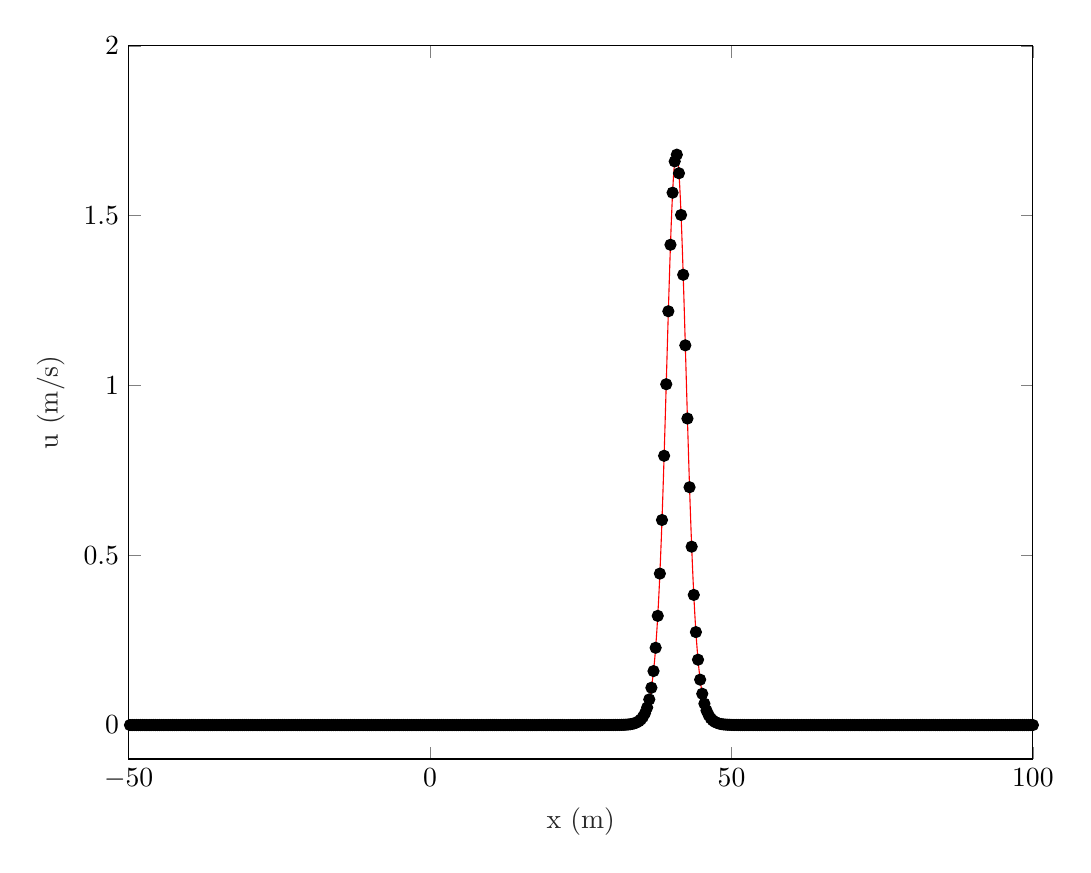
\begin{tikzpicture}

\begin{axis}[%
width=4.521in,
height=3.566in,
at={(0.758in,0.481in)},
scale only axis,
xmin=-50,
xmax=100,
xtick={-50,   0,  50, 100},
xlabel style={font=\color{white!15!black}},
xlabel={x (m)},
ymin=-0.1,
ymax=2,
ytick={  0, 0.5,   1, 1.5,   2},
ylabel style={font=\color{white!15!black}},
ylabel={u (m/s)},
axis background/.style={fill=white}
]
\addplot [color=red, forget plot]
  table[row sep=crcr]{%
-50.14064697609	0\\
-50.0234411626817	0\\
-49.9062353492733	0\\
-49.789029535865	0\\
-49.6718237224566	0\\
-49.5546179090483	0\\
-49.4374120956399	0\\
-49.3202062822316	0\\
-49.2030004688233	0\\
-49.0857946554149	0\\
-48.9685888420066	0\\
-48.8513830285982	0\\
-48.7341772151899	0\\
-48.6169714017815	0\\
-48.4997655883732	0\\
-48.3825597749648	0\\
-48.2653539615565	0\\
-48.1481481481481	0\\
-48.0309423347398	0\\
-47.9137365213315	0\\
-47.7965307079231	0\\
-47.6793248945148	0\\
-47.5621190811064	0\\
-47.4449132676981	0\\
-47.3277074542897	0\\
-47.2105016408814	0\\
-47.093295827473	0\\
-46.9760900140647	0\\
-46.8588842006564	0\\
-46.741678387248	0\\
-46.6244725738397	0\\
-46.5072667604313	0\\
-46.390060947023	0\\
-46.2728551336146	0\\
-46.1556493202063	0\\
-46.0384435067979	0\\
-45.9212376933896	0\\
-45.8040318799812	0\\
-45.6868260665729	0\\
-45.5696202531646	0\\
-45.4524144397562	0\\
-45.3352086263479	0\\
-45.2180028129395	0\\
-45.1007969995312	0\\
-44.9835911861228	0\\
-44.8663853727145	0\\
-44.7491795593061	0\\
-44.6319737458978	0\\
-44.5147679324894	0\\
-44.3975621190811	0\\
-44.2803563056728	0\\
-44.1631504922644	0\\
-44.0459446788561	0\\
-43.9287388654477	0\\
-43.8115330520394	0\\
-43.694327238631	0\\
-43.5771214252227	0\\
-43.4599156118143	0\\
-43.342709798406	0\\
-43.2255039849977	0\\
-43.1082981715893	0\\
-42.991092358181	0\\
-42.8738865447726	0\\
-42.7566807313643	0\\
-42.6394749179559	0\\
-42.5222691045476	0\\
-42.4050632911392	0\\
-42.2878574777309	0\\
-42.1706516643225	0\\
-42.0534458509142	0\\
-41.9362400375059	0\\
-41.8190342240975	0\\
-41.7018284106892	0\\
-41.5846225972808	0\\
-41.4674167838725	0\\
-41.3502109704641	0\\
-41.2330051570558	0\\
-41.1157993436474	0\\
-40.9985935302391	0\\
-40.8813877168308	0\\
-40.7641819034224	0\\
-40.6469760900141	0\\
-40.5297702766057	0\\
-40.4125644631974	0\\
-40.295358649789	0\\
-40.1781528363807	0\\
-40.0609470229723	0\\
-39.943741209564	0\\
-39.8265353961556	0\\
-39.7093295827473	0\\
-39.592123769339	0\\
-39.4749179559306	0\\
-39.3577121425223	0\\
-39.2405063291139	0\\
-39.1233005157056	0\\
-39.0060947022972	0\\
-38.8888888888889	0\\
-38.7716830754805	0\\
-38.6544772620722	0\\
-38.5372714486639	0\\
-38.4200656352555	0\\
-38.3028598218472	0\\
-38.1856540084388	0\\
-38.0684481950305	0\\
-37.9512423816221	0\\
-37.8340365682138	0\\
-37.7168307548054	0\\
-37.5996249413971	0\\
-37.4824191279887	0\\
-37.3652133145804	0\\
-37.2480075011721	0\\
-37.1308016877637	0\\
-37.0135958743554	0\\
-36.896390060947	0\\
-36.7791842475387	0\\
-36.6619784341303	0\\
-36.544772620722	0\\
-36.4275668073136	0\\
-36.3103609939053	0\\
-36.193155180497	0\\
-36.0759493670886	0\\
-35.9587435536803	0\\
-35.8415377402719	0\\
-35.7243319268636	0\\
-35.6071261134552	0\\
-35.4899203000469	0\\
-35.3727144866385	0\\
-35.2555086732302	0\\
-35.1383028598218	0\\
-35.0210970464135	0\\
-34.9038912330052	0\\
-34.7866854195968	0\\
-34.6694796061885	0\\
-34.5522737927801	0\\
-34.4350679793718	0\\
-34.3178621659634	0\\
-34.2006563525551	0\\
-34.0834505391467	0\\
-33.9662447257384	0\\
-33.8490389123301	0\\
-33.7318330989217	0\\
-33.6146272855134	0\\
-33.497421472105	0\\
-33.3802156586967	0\\
-33.2630098452883	0\\
-33.14580403188	0\\
-33.0285982184716	0\\
-32.9113924050633	0\\
-32.7941865916549	0\\
-32.6769807782466	0\\
-32.5597749648383	0\\
-32.4425691514299	0\\
-32.3253633380216	0\\
-32.2081575246132	0\\
-32.0909517112049	0\\
-31.9737458977965	0\\
-31.8565400843882	0\\
-31.7393342709798	0\\
-31.6221284575715	0\\
-31.5049226441632	0\\
-31.3877168307548	0\\
-31.2705110173465	0\\
-31.1533052039381	0\\
-31.0360993905298	0\\
-30.9188935771214	0\\
-30.8016877637131	0\\
-30.6844819503047	0\\
-30.5672761368964	0\\
-30.450070323488	0\\
-30.3328645100797	0\\
-30.2156586966714	0\\
-30.098452883263	0\\
-29.9812470698547	0\\
-29.8640412564463	0\\
-29.746835443038	0\\
-29.6296296296296	0\\
-29.5124238162213	0\\
-29.3952180028129	0\\
-29.2780121894046	0\\
-29.1608063759962	0\\
-29.0436005625879	0\\
-28.9263947491796	0\\
-28.8091889357712	0\\
-28.6919831223629	0\\
-28.5747773089545	0\\
-28.4575714955462	0\\
-28.3403656821378	0\\
-28.2231598687295	0\\
-28.1059540553211	0\\
-27.9887482419128	0\\
-27.8715424285045	0\\
-27.7543366150961	0\\
-27.6371308016878	0\\
-27.5199249882794	0\\
-27.4027191748711	0\\
-27.2855133614627	0\\
-27.1683075480544	0\\
-27.051101734646	0\\
-26.9338959212377	0\\
-26.8166901078293	0\\
-26.699484294421	0\\
-26.5822784810127	0\\
-26.4650726676043	0\\
-26.347866854196	0\\
-26.2306610407876	0\\
-26.1134552273793	0\\
-25.9962494139709	0\\
-25.8790436005626	0\\
-25.7618377871542	0\\
-25.6446319737459	0\\
-25.5274261603376	0\\
-25.4102203469292	0\\
-25.2930145335209	0\\
-25.1758087201125	0\\
-25.0586029067042	0\\
-24.9413970932958	0\\
-24.8241912798875	0\\
-24.7069854664791	0\\
-24.5897796530708	0\\
-24.4725738396624	0\\
-24.3553680262541	0\\
-24.2381622128458	0\\
-24.1209563994374	0\\
-24.0037505860291	0\\
-23.8865447726207	0\\
-23.7693389592124	0\\
-23.652133145804	0\\
-23.5349273323957	0\\
-23.4177215189873	0\\
-23.300515705579	0\\
-23.1833098921707	0\\
-23.0661040787623	0\\
-22.948898265354	0\\
-22.8316924519456	0\\
-22.7144866385373	0\\
-22.5972808251289	0\\
-22.4800750117206	0\\
-22.3628691983122	0\\
-22.2456633849039	0\\
-22.1284575714955	0\\
-22.0112517580872	0\\
-21.8940459446789	0\\
-21.7768401312705	0\\
-21.6596343178622	0\\
-21.5424285044538	0\\
-21.4252226910455	0\\
-21.3080168776371	0\\
-21.1908110642288	0\\
-21.0736052508204	0\\
-20.9563994374121	0\\
-20.8391936240038	0\\
-20.7219878105954	0\\
-20.6047819971871	0\\
-20.4875761837787	0\\
-20.3703703703704	0\\
-20.253164556962	0\\
-20.1359587435537	0\\
-20.0187529301453	0\\
-19.901547116737	0\\
-19.7843413033286	0\\
-19.6671354899203	0\\
-19.549929676512	0\\
-19.4327238631036	0\\
-19.3155180496953	0\\
-19.1983122362869	0\\
-19.0811064228786	0\\
-18.9639006094702	0\\
-18.8466947960619	0\\
-18.7294889826535	0\\
-18.6122831692452	0\\
-18.4950773558368	0\\
-18.3778715424285	0\\
-18.2606657290202	0\\
-18.1434599156118	0\\
-18.0262541022035	0\\
-17.9090482887951	0\\
-17.7918424753868	0\\
-17.6746366619784	0\\
-17.5574308485701	0\\
-17.4402250351617	0\\
-17.3230192217534	0\\
-17.2058134083451	0\\
-17.0886075949367	0\\
-16.9714017815284	0\\
-16.85419596812	0\\
-16.7369901547117	0\\
-16.6197843413033	0\\
-16.502578527895	0\\
-16.3853727144866	0\\
-16.2681669010783	0\\
-16.1509610876699	0\\
-16.0337552742616	0\\
-15.9165494608533	0\\
-15.7993436474449	0\\
-15.6821378340366	0\\
-15.5649320206282	0\\
-15.4477262072199	0\\
-15.3305203938115	0\\
-15.2133145804032	0\\
-15.0961087669948	0\\
-14.9789029535865	0\\
-14.8616971401782	0\\
-14.7444913267698	0\\
-14.6272855133615	0\\
-14.5100796999531	0\\
-14.3928738865448	0\\
-14.2756680731364	0\\
-14.1584622597281	0\\
-14.0412564463197	0\\
-13.9240506329114	0\\
-13.806844819503	0\\
-13.6896390060947	0\\
-13.5724331926864	0\\
-13.455227379278	0\\
-13.3380215658697	0\\
-13.2208157524613	0\\
-13.103609939053	0\\
-12.9864041256446	0\\
-12.8691983122363	0\\
-12.7519924988279	0\\
-12.6347866854196	0\\
-12.5175808720113	0\\
-12.4003750586029	0\\
-12.2831692451946	0\\
-12.1659634317862	0\\
-12.0487576183779	0\\
-11.9315518049695	0\\
-11.8143459915612	0\\
-11.6971401781528	0\\
-11.5799343647445	0\\
-11.4627285513361	0\\
-11.3455227379278	0\\
-11.2283169245195	0\\
-11.1111111111111	0\\
-10.9939052977028	0\\
-10.8766994842944	0\\
-10.7594936708861	0\\
-10.6422878574777	0\\
-10.5250820440694	0\\
-10.407876230661	0\\
-10.2906704172527	0\\
-10.1734646038444	0\\
-10.056258790436	0\\
-9.93905297702766	0\\
-9.82184716361932	0\\
-9.70464135021097	0\\
-9.58743553680262	0\\
-9.47022972339428	0\\
-9.35302390998594	0\\
-9.23581809657759	0\\
-9.11861228316924	0\\
-9.0014064697609	0\\
-8.88420065635255	0\\
-8.76699484294421	0\\
-8.64978902953587	0\\
-8.53258321612752	0\\
-8.41537740271917	0\\
-8.29817158931083	0\\
-8.18096577590249	0\\
-8.06375996249414	0\\
-7.94655414908579	0\\
-7.82934833567745	0\\
-7.7121425222691	0\\
-7.59493670886076	0\\
-7.47773089545242	0\\
-7.36052508204407	0\\
-7.24331926863572	0\\
-7.12611345522738	0\\
-7.00890764181904	0\\
-6.89170182841069	0\\
-6.77449601500234	0\\
-6.657290201594	0\\
-6.54008438818565	0\\
-6.42287857477731	0\\
-6.30567276136896	0\\
-6.18846694796062	0\\
-6.07126113455227	0\\
-5.95405532114393	0\\
-5.83684950773559	0\\
-5.71964369432724	0\\
-5.60243788091889	0\\
-5.48523206751055	0\\
-5.3680262541022	0\\
-5.25082044069386	0\\
-5.13361462728551	0\\
-5.01640881387717	0\\
-4.89920300046882	0\\
-4.78199718706048	0\\
-4.66479137365214	0\\
-4.54758556024379	0\\
-4.43037974683544	0\\
-4.31317393342709	0\\
-4.19596812001875	0\\
-4.07876230661041	0\\
-3.96155649320206	0\\
-3.84435067979372	0\\
-3.72714486638537	0\\
-3.60993905297703	0\\
-3.49273323956868	0\\
-3.37552742616034	0\\
-3.25832161275199	0\\
-3.14111579934364	0\\
-3.0239099859353	0\\
-2.90670417252696	0\\
-2.78949835911861	0\\
-2.67229254571027	0\\
-2.55508673230192	0\\
-2.43788091889358	0\\
-2.32067510548523	0\\
-2.20346929207689	0\\
-2.08626347866854	0\\
-1.96905766526019	0\\
-1.85185185185185	0\\
-1.73464603844351	0\\
-1.61744022503516	0\\
-1.50023441162681	0\\
-1.38302859821847	0\\
-1.26582278481013	0\\
-1.14861697140178	0\\
-1.03141115799344	0\\
-0.914205344585092	0\\
-0.796999531176745	0\\
-0.679793717768398	0\\
-0.562587904360058	0\\
-0.445382090951711	0\\
-0.328176277543363	0\\
-0.210970464135023	0\\
-0.0937646507266763	0\\
0.0234411626816708	0\\
0.140646976090011	0\\
0.257852789498358	0\\
0.375058602906705	0\\
0.492264416315052	0\\
0.609470229723392	0\\
0.726676043131739	0\\
0.843881856540087	0\\
0.961087669948427	0\\
1.07829348335677	0\\
1.19549929676512	0\\
1.31270511017347	0\\
1.42991092358181	0\\
1.54711673699016	0\\
1.6643225503985	0\\
1.78152836380684	0\\
1.89873417721519	0\\
2.01593999062354	0\\
2.13314580403188	0\\
2.25035161744022	0\\
2.36755743084857	0\\
2.48476324425692	0\\
2.60196905766526	0\\
2.71917487107361	0\\
2.83638068448195	0\\
2.95358649789029	0\\
3.07079231129864	0\\
3.18799812470699	0\\
3.30520393811533	0\\
3.42240975152367	0\\
3.53961556493202	0\\
3.65682137834037	0\\
3.77402719174871	0\\
3.89123300515705	0\\
4.0084388185654	0\\
4.12564463197375	0\\
4.24285044538209	0\\
4.36005625879044	0\\
4.47726207219878	0\\
4.59446788560712	0\\
4.71167369901547	0\\
4.82887951242382	0\\
4.94608532583216	0\\
5.0632911392405	0\\
5.18049695264885	0\\
5.2977027660572	0\\
5.41490857946554	0\\
5.53211439287389	0\\
5.64932020628223	0\\
5.76652601969058	0\\
5.88373183309892	0\\
6.00093764650727	0\\
6.11814345991561	0\\
6.23534927332395	0\\
6.3525550867323	0\\
6.46976090014065	0\\
6.58696671354899	0\\
6.70417252695734	0\\
6.82137834036568	0\\
6.93858415377403	9.06774273054312e-16\\
7.05578996718237	9.06774273054312e-16\\
7.17299578059072	9.06774273054312e-16\\
7.29020159399906	9.06774273054312e-16\\
7.4074074074074	9.06774273054312e-16\\
7.52461322081575	9.06774273054312e-16\\
7.6418190342241	9.06774273054312e-16\\
7.75902484763245	9.06774273054312e-16\\
7.87623066104079	1.81354854610862e-15\\
7.99343647444913	1.81354854610862e-15\\
8.11064228785748	1.81354854610862e-15\\
8.22784810126582	1.81354854610862e-15\\
8.34505391467417	2.72032281916294e-15\\
8.46225972808251	2.72032281916294e-15\\
8.57946554149086	2.72032281916294e-15\\
8.6966713548992	3.62709709221725e-15\\
8.81387716830755	3.62709709221725e-15\\
8.9310829817159	4.53387136527156e-15\\
9.04828879512424	5.44064563832587e-15\\
9.16549460853258	5.44064563832587e-15\\
9.28270042194093	6.34741991138018e-15\\
9.39990623534927	7.2541941844345e-15\\
9.51711204875762	9.06774273054312e-15\\
9.63431786216596	9.97451700359743e-15\\
9.75152367557431	1.08812912766517e-14\\
9.86872948898265	1.26948398227604e-14\\
9.985935302391	1.4508388368869e-14\\
10.1031411157993	1.63219369149776e-14\\
10.2203469292077	1.90422597341406e-14\\
10.337552742616	2.17625825533035e-14\\
10.4547585560244	2.44829053724664e-14\\
10.5719643694327	2.81100024646837e-14\\
10.6891701828411	3.17370995569009e-14\\
10.8063759962494	3.62709709221725e-14\\
10.9235818096578	4.0804842287444e-14\\
11.0407876230661	4.71522621988242e-14\\
11.1579934364744	5.34996821102044e-14\\
11.2751992498828	6.07538762946389e-14\\
11.3924050632911	6.89148447521277e-14\\
11.5096108766995	7.88893617557252e-14\\
11.6268166901078	8.97706530323769e-14\\
11.7440225035162	1.02465492855137e-13\\
11.8612283169245	1.16973881224006e-13\\
11.9784341303329	1.33295818138984e-13\\
12.0956399437412	1.5143130360007e-13\\
12.2128457571496	1.72287111880319e-13\\
12.3300515705579	1.96770017252786e-13\\
12.4472573839662	2.23973245444415e-13\\
12.5644631973746	2.54803570728262e-13\\
12.6816690107829	2.91074541650434e-13\\
12.7988748241913	3.30972609664824e-13\\
12.9160806375996	3.77218097590594e-13\\
13.033286451008	4.29811005427744e-13\\
13.1504922644163	4.89658107449328e-13\\
13.2676980778247	5.57666177928402e-13\\
13.384903891233	6.34741991138018e-13\\
13.5021097046413	7.23605869897341e-13\\
13.6193155180497	8.2425781420637e-13\\
13.736521331458	9.38511372611213e-13\\
13.8537271448664	1.06908686793103e-12\\
13.9709329582747	1.218704622985e-12\\
14.0881387716831	1.3873646377731e-12\\
14.2053445850914	1.58050755793367e-12\\
14.3225503984998	1.80085370628586e-12\\
14.4397562119081	2.05112340564885e-12\\
14.5569620253165	2.33675730166096e-12\\
14.6741678387248	2.66228926568746e-12\\
14.7913736521331	3.03225316909362e-12\\
14.9085794655415	3.45390320606387e-12\\
15.0257852789498	3.93449357078266e-12\\
15.1429910923582	4.48218523170746e-12\\
15.2601969057665	5.10604593156883e-12\\
15.3774027191749	5.81605018737036e-12\\
15.4946085325832	6.62579961320786e-12\\
15.6118143459916	7.54708227463104e-12\\
15.7290201593999	8.59712688282793e-12\\
15.8462259728083	9.79316214898657e-12\\
15.9634317862166	1.11560438813872e-11\\
16.0806375996249	1.27084414368562e-11\\
16.1978434130333	1.44766512693121e-11\\
16.3150492264416	1.64905969297657e-11\\
16.43225503985	1.87847358405931e-11\\
16.5494608532583	2.13980592955357e-11\\
16.6666666666667	2.4375906008246e-11\\
16.783872480075	2.77672417894691e-11\\
16.9010782934834	3.16301001926805e-11\\
17.0182841068917	3.60306757398131e-11\\
17.1354899203	4.10442306955304e-11\\
17.2526957337084	4.67541882929534e-11\\
17.3699015471167	5.3259386927845e-11\\
17.4871073605251	6.06695462872449e-11\\
17.6043131739334	6.91107079951074e-11\\
17.7215189873418	7.87261423865754e-11\\
17.8387248007501	8.96799756050715e-11\\
17.9559306141585	1.02157189602299e-10\\
18.0731364275668	1.16370876332425e-10\\
18.1903422409752	1.32562237752083e-10\\
18.3075480543835	1.51005119691735e-10\\
18.4247538677918	1.72015079598403e-10\\
18.5419596812002	1.95948479761398e-10\\
18.6591654946085	2.23210648280776e-10\\
18.7763713080169	2.54266760358614e-10\\
18.8935771214252	2.89643651847554e-10\\
19.0107829348336	3.29942514090634e-10\\
19.1279887482419	3.75847961664009e-10\\
19.2451945616503	4.28140727216778e-10\\
19.3624003750586	4.87708542762262e-10\\
19.4796061884669	5.55565181937735e-10\\
19.5968120018753	6.32862248069977e-10\\
19.7140178152836	7.20913657080643e-10\\
19.831223628692	8.21216493294545e-10\\
19.9484294421003	9.35474585570754e-10\\
20.0656352555087	1.06562933762788e-09\\
20.182841068917	1.2138923719179e-09\\
20.3000468823254	1.3827845209199e-09\\
20.4172526957337	1.57517481843383e-09\\
20.5344585091421	1.79433218571406e-09\\
20.6516643225504	2.04398255824855e-09\\
20.7688701359587	2.32836691931239e-09\\
20.8860759493671	2.65231837578095e-09\\
21.0032817627754	3.02134195426596e-09\\
21.1204875761838	3.44170890563984e-09\\
21.2376933895921	3.92056189085145e-09\\
21.3548992030005	4.46603920900146e-09\\
21.4721050164088	5.08741081348329e-09\\
21.5893108298172	5.79523427715812e-09\\
21.7065166432255	6.60153977430656e-09\\
21.8237224566338	7.52002866419446e-09\\
21.9409282700422	8.56630834560963e-09\\
22.0581340834505	9.7581597552724e-09\\
22.1753398968589	1.11158366033457e-08\\
22.2925457102672	1.26624108544331e-08\\
22.4097515236756	1.44241635472906e-08\\
22.5269573370839	1.64310327413173e-08\\
22.6441631504923	1.87171222169228e-08\\
22.7613689639006	2.13212818110619e-08\\
22.878574777309	2.42877648285823e-08\\
22.9957805907173	2.76669815716461e-08\\
23.1129864041256	3.151635578803e-08\\
23.230192217534	3.5901304894115e-08\\
23.3473980309423	4.0896341705628e-08\\
23.4646038443507	4.65863502690438e-08\\
23.581809657759	5.30680240055825e-08\\
23.6990154711674	6.04515087861918e-08\\
23.8162212845757	6.88622758738088e-08\\
23.9334270979841	7.84432546564492e-08\\
24.0506329113924	8.93572573616143e-08\\
24.1678387248007	1.01789751972017e-07\\
24.2850445382091	1.15952011452635e-07\\
24.4022503516174	1.32084700042954e-07\\
24.5194561650258	1.50461968249595e-07\\
24.6366619784341	1.71396111852519e-07\\
24.7538677918425	1.95242872907434e-07\\
24.8710736052508	2.2240749337084e-07\\
24.9882794186592	2.53351593436275e-07\\
25.1054852320675	2.88601021479201e-07\\
25.2226910454759	3.2875478759714e-07\\
25.3398968588842	3.74495244871209e-07\\
25.4571026722925	4.26599682475207e-07\\
25.5743084857009	4.85953536469996e-07\\
25.6915142991092	5.53565434548849e-07\\
25.8087201125176	6.30584339058476e-07\\
25.9259259259259	7.18319067128794e-07\\
26.0431317393343	8.18260536112787e-07\\
26.1603375527426	9.32107098406299e-07\\
26.277543366151	1.06179340089945e-06\\
26.3947491795593	1.20952326053126e-06\\
26.5119549929676	1.37780711769429e-06\\
26.629160806376	1.56950469452345e-06\\
26.7463666197843	1.78787358983615e-06\\
26.8635724331927	2.03662463996857e-06\\
26.980778246601	2.31998497313827e-06\\
27.0979840600094	2.64276984682245e-06\\
27.2151898734177	3.01046446917432e-06\\
27.3323956868261	3.42931721405818e-06\\
27.4496015002344	3.90644579388892e-06\\
27.5668073136428	4.44995821787938e-06\\
27.6840131270511	5.06909056369633e-06\\
27.8012189404594	5.77436392739224e-06\\
27.9184247538678	6.57776320528796e-06\\
28.0356305672761	7.49294074640665e-06\\
28.1528363806845	8.53544833888351e-06\\
28.2700421940928	9.72300147209892e-06\\
28.3872480075012	1.10757803598941e-05\\
28.5044538209095	1.26167728395292e-05\\
28.6216596343179	1.43721649746762e-05\\
28.7388654477262	1.63717859945929e-05\\
28.8560712611346	1.86496151297085e-05\\
28.9732770745429	2.12443589439223e-05\\
29.0904828879512	2.42001089776323e-05\\
29.2076887013596	2.7567090867513e-05\\
29.3248945147679	3.14025176564703e-05\\
29.4421003281763	3.57715617881077e-05\\
29.5593061415846	4.07484622794739e-05\\
29.676511954993	4.64177858754163e-05\\
29.7937177684013	5.28758635689993e-05\\
29.9109235818097	6.02324268779463e-05\\
30.028129395218	6.8612471626214e-05\\
30.1453352086263	7.81583808349547e-05\\
30.2625410220347	8.90323427240722e-05\\
30.379746835443	0.000101419104795608\\
30.4969526488514	0.00011552911067516\\
30.6141584622597	0.000131602072815669\\
30.7313642756681	0.000149911041553117\\
30.8485700890764	0.00017076703935599\\
30.9657759024848	0.000194524338611991\\
31.0829817158931	0.000221586472133703\\
31.2001875293015	0.000252413077847617\\
31.3173933427098	0.000287527693114307\\
31.4345991561181	0.000327526630003336\\
31.5518049695265	0.000373089080882208\\
31.6690107829348	0.000424988624155939\\
31.7862165963432	0.000484106323209475\\
31.9034224097515	0.000551445637959232\\
32.0206282231599	0.000628149398278317\\
32.1378340365682	0.000715519122346805\\
32.2550398499766	0.000815037001262058\\
32.3722456633849	0.000928390914450008\\
32.4894514767932	0.00105750288927762\\
32.6066572902016	0.00120456147328252\\
32.7238631036099	0.00137205854946016\\
32.8410689170183	0.00156283119467619\\
32.9582747304266	0.00178010925943831\\
33.075480543835	0.00202756943468269\\
33.1926863572433	0.00230939666879157\\
33.3098921706517	0.00263035390653889\\
33.42709798406	0.002995861241836\\
33.5443037974684	0.00341208570866381\\
33.6615096108767	0.00388604307979318\\
33.778715424285	0.00442571320104597\\
33.8959212376934	0.00504017055957566\\
34.0131270511017	0.00573973196690971\\
34.1303328645101	0.00653612342967975\\
34.2475386779184	0.00744266847969811\\
34.3647444913268	0.00847450043594509\\
34.4819503047351	0.00964880126703259\\
34.5991561181435	0.0109850699041282\\
34.7163619315518	0.0125054230078522\\
34.8335677449601	0.0142349312998318\\
34.9507735583685	0.0162019946063359\\
35.0679793717768	0.0184387586954479\\
35.1851851851852	0.0209815767790725\\
35.3023909985935	0.0238715181430804\\
35.4195968120019	0.0271549256952327\\
35.5368026254102	0.0308840231960466\\
35.6540084388186	0.0351175714574539\\
35.7712142522269	0.0399215707299474\\
35.8884200656353	0.0453700036984107\\
36.0056258790436	0.0515456097915298\\
36.122831692452	0.0585406766774211\\
36.2400375058603	0.066457828647872\\
36.3572433192686	0.0754107838569794\\
36.474449132677	0.0855250428609074\\
36.5916549460853	0.0969384594317847\\
36.7088607594937	0.109801631109072\\
36.826066572902	0.124278031483017\\
36.9432723863104	0.140543789101873\\
37.0604781997187	0.158786999845292\\
37.177684013127	0.179206441798467\\
37.2948898265354	0.202009545932535\\
37.4120956399437	0.22740946487397\\
37.5293014533521	0.255621079244283\\
37.6465072667604	0.28685579086935\\
37.7637130801688	0.321314979698232\\
37.8809188935771	0.359182051898698\\
37.9981247069855	0.400613085141572\\
38.1153305203938	0.445726186646318\\
38.2325363338022	0.494589819921988\\
38.3497421472105	0.547210521986804\\
38.4669479606189	0.603520612124091\\
38.5841537740272	0.663366666180676\\
38.7013595874355	0.72649967006103\\
38.8185654008439	0.792567840764187\\
38.9357712142522	0.861113081704344\\
39.0529770276606	0.931571897213825\\
39.1701828410689	1.00328132053016\\
39.2873886544773	1.07549002388592\\
39.4045944678856	1.14737431737289\\
39.5218002812939	1.21805826602\\
39.6390060947023	1.28663673549676\\
39.7562119081106	1.35219988723851\\
39.873417721519	1.41385753620772\\
39.9906235349273	1.47076187989757\\
40.1078293483357	1.52212738904434\\
40.225035161744	1.56724706833021\\
40.3422409751524	1.60550477611835\\
40.4594467885607	1.63638375643018\\
40.5766526019691	1.65947191363387\\
40.6938584153774	1.67446460119774\\
40.8110642287858	1.68116577729349\\
40.9282700421941	1.679488304982\\
41.0454758556024	1.66945396779611\\
41.1626816690108	1.65119347281564\\
41.2798874824191	1.62494637213412\\
41.3970932958275	1.59106050313487\\
41.5142991092358	1.54999028046363\\
41.6315049226442	1.50229301432615\\
41.7487107360525	1.44862241540816\\
41.8659165494608	1.38971859296451\\
41.9831223628692	1.32639415235617\\
42.1003281762775	1.25951641763248\\
42.2175339896859	1.18998628483471\\
42.3347398030942	1.11871467683508\\
42.4519456165026	1.04659794179064\\
42.5691514299109	0.974493748905007\\
42.6863572433193	0.903199049253638\\
42.8035630567276	0.833431484522666\\
42.920768870136	0.765815277425135\\
43.0379746835443	0.7008721862066\\
43.1551804969527	0.639017626126788\\
43.272386310361	0.580561623139842\\
43.3895921237693	0.525713922101334\\
43.5067979371777	0.474592352456931\\
43.624003750586	0.427233462682169\\
43.7412095639944	0.383604455121435\\
43.8584153774027	0.343615557468145\\
43.9756211908111	0.307132123716976\\
44.0928270042194	0.273985935762325\\
44.2100328176277	0.243985352652912\\
44.3272386310361	0.216924111204356\\
44.4444444444444	0.192588710024351\\
44.5616502578528	0.170764405960209\\
44.6788560712611	0.151239918856142\\
44.7960618846695	0.133810981268217\\
44.9132676980778	0.118282889593725\\
45.0304735114862	0.104472217262382\\
45.1476793248945	0.0922078440667746\\
45.2648851383029	0.0813314424334248\\
45.3820909517112	0.0716975446069546\\
45.4992967651196	0.0631732966348332\\
45.6165025785279	0.0556379872581005\\
45.7337083919362	0.0489824233049075\\
45.8509142053446	0.0431082084757877\\
45.9681200187529	0.0379269697156838\\
46.0853258321613	0.0333595646920224\\
46.2025316455696	0.0293352951160212\\
46.319737458978	0.0257911435615636\\
46.4369432723863	0.0226710458282338\\
46.5541490857947	0.0199252065352604\\
46.671354899203	0.0175094623067961\\
46.7885607126113	0.0153846944228922\\
46.9057665260197	0.01351629099686\\
47.022972339428	0.0118736574557193\\
47.1401781528364	0.0104297732277176\\
47.2573839662447	0.00916079198268795\\
47.3745897796531	0.00804568244945439\\
47.4917955930614	0.00706590668768253\\
47.6090014064698	0.00620513267114321\\
47.7262072198781	0.00544897810760407\\
47.8434130332865	0.00478478254886827\\
47.9606188466948	0.00420140501100139\\
48.0778246601031	0.00368904451347711\\
48.1950304735115	0.00323908114488455\\
48.3122362869198	0.00284393546359155\\
48.4294421003282	0.00249694423831388\\
48.5466479137365	0.00219225072204547\\
48.6638537271449	0.00192470783064548\\
48.7810595405532	0.00168979276311278\\
48.8982653539616	0.00148353175357757\\
49.0154711673699	0.00130243378515719\\
49.1326769807782	0.00114343222330498\\
49.2498827941866	0.00100383344171454\\
49.3670886075949	0.000881271617858047\\
49.4842944210033	0.000773668968633056\\
49.6015002344116	0.000679200780229493\\
49.71870604782	0.000596264660961034\\
49.8359118612283	0.000523453512314844\\
49.9531176746367	0.000459531772598186\\
50.070323488045	0.000403414540043558\\
50.1875293014534	0.000354149228735224\\
50.3047351148617	0.000310899451916122\\
50.42194092827	0.000272930863634315\\
50.5391467416784	0.000239598721858688\\
50.6563525550867	0.000210336964605091\\
50.7735583684951	0.000184648615646573\\
50.8907641819034	0.000162097358477567\\
51.0079699953118	0.000142300136678561\\
51.1251758087201	0.00012492065592359\\
51.2423816221285	0.000109663678018346\\
51.3595874355368	9.62700105928315e-05\\
51.4767932489451	8.45121077680922e-05\\
51.5939990623535	7.41902074147901e-05\\
51.7112048757618	6.51289396111296e-05\\
51.8284106891702	5.71743489067714e-05\\
51.9456165025785	5.01912799321048e-05\\
52.0628223159869	4.40610820660213e-05\\
52.1800281293952	3.86795942493338e-05\\
52.2972339428036	3.39553757725054e-05\\
52.4144397562119	2.98081530316197e-05\\
52.5316455696203	2.61674559040006e-05\\
52.6488513830286	2.29714206021477e-05\\
52.7660571964369	2.01657386928834e-05\\
52.8832630098453	1.77027344350346e-05\\
53.0004688232536	1.55405547838175e-05\\
53.117674636662	1.36424582934657e-05\\
53.2348804500703	1.19761908607231e-05\\
53.3520862634787	1.05134376963164e-05\\
53.469292076887	9.22934221546216e-06\\
53.5864978902954	8.10208369414741e-06\\
53.7037037037037	7.11250648867616e-06\\
53.820909517112	6.24379454632367e-06\\
53.9381153305204	5.48118566353429e-06\\
54.0553211439287	4.8117206426874e-06\\
54.1725269573371	4.22402307924488e-06\\
54.2897327707454	3.70810605334463e-06\\
54.4069385841538	3.25520241656744e-06\\
54.5241443975621	2.85761582161884e-06\\
54.6413502109705	2.50858993510192e-06\\
54.7585560243788	2.20219362674614e-06\\
54.8757618377872	1.93322018280707e-06\\
54.9929676511955	1.69709882847348e-06\\
55.1101734646038	1.48981705448983e-06\\
55.2273792780122	1.30785243362502e-06\\
55.3445850914205	1.1481127608755e-06\\
55.4617909048289	1.00788350952327e-06\\
55.5789967182372	8.8478170126165e-07\\
55.6962025316456	7.76715410563015e-07\\
55.8134083450539	6.81848216860387e-07\\
55.9306141584623	5.98567998817575e-07\\
56.0478199718706	5.25459535691138e-07\\
56.165025785279	4.61280461943597e-07\\
56.2822315986873	4.04940150737552e-07\\
56.3994374120956	3.55481184910186e-07\\
56.516643225504	3.1206308400216e-07\\
56.6338490389123	2.73948025283137e-07\\
56.7510548523207	2.40488298529712e-07\\
56.868260665729	2.11115308667032e-07\\
56.9854664791374	1.8532990320762e-07\\
57.1026722925457	1.6269390161951e-07\\
57.2198781059541	1.4282263756123e-07\\
57.3370839193624	1.25378428293497e-07\\
57.4542897327707	1.10064836611609e-07\\
57.5714955461791	9.66216314474252e-08\\
57.6887013595874	8.48203655312391e-08\\
57.8059071729958	7.44604934911119e-08\\
57.9231129864041	6.53659660087041e-08\\
58.0403187998125	5.7382233837078e-08\\
58.1575246132208	5.03736272230475e-08\\
58.2747304266292	4.42210449929443e-08\\
58.3919362400375	3.88199319926007e-08\\
58.5091420534459	3.40785054368727e-08\\
58.6263478668542	2.99161916307922e-08\\
58.7435536802625	2.62622594607382e-08\\
58.8607594936709	2.3054613477879e-08\\
58.9779653070792	2.02387474806614e-08\\
59.0951711204876	1.77668073635993e-08\\
59.2123769338959	1.55967877152675e-08\\
59.3295827473043	1.36918118395297e-08\\
59.4467885607126	1.20195088016119e-08\\
59.563994374121	1.05514575754739e-08\\
59.6812001875293	9.26271370763817e-09\\
59.7984060009376	8.13137587908768e-09\\
59.915611814346	7.13821775491085e-09\\
60.0328176277543	6.26636335911186e-09\\
60.1500234411627	5.500996000069e-09\\
60.267229254571	4.82910981438386e-09\\
60.3844350679794	4.23928760718441e-09\\
60.5016408813877	3.72150498888202e-09\\
60.6188466947961	3.26696443547954e-09\\
60.7360525082044	2.86794113694481e-09\\
60.8532583216128	2.51765332848966e-09\\
60.9704641350211	2.21014985056003e-09\\
61.0876699484294	1.94020405624603e-09\\
61.2048757618378	1.70322948127456e-09\\
61.3220815752461	1.49519914109899e-09\\
61.4392873886545	1.3125766160544e-09\\
61.5564932020628	1.15225983135267e-09\\
61.6736990154712	1.01152393030327e-09\\
61.7909048288795	8.87977749148169e-10\\
61.9081106422879	7.79521198670962e-10\\
62.0253164556962	6.84310806774532e-10\\
62.1425222691045	6.00729794930024e-10\\
62.2597280825129	5.27357247851561e-10\\
62.3769338959212	4.62946350913695e-10\\
62.4941397093296	4.06402627568847e-10\\
62.6113455227379	3.56764897087581e-10\\
62.7285513361463	3.13189859395956e-10\\
62.8457571495546	2.7493758668716e-10\\
62.962962962963	2.41357015033139e-10\\
63.0801687763713	2.11877783416144e-10\\
63.1973745897797	1.85999352437447e-10\\
63.314580403188	1.63281936574617e-10\\
63.4317862165964	1.4333834321306e-10\\
63.5489920300047	1.25831252323201e-10\\
63.666197843413	1.10462335169203e-10\\
63.7834036568214	9.69704407604281e-11\\
63.9006094702297	8.51270619800658e-11\\
64.0178152836381	7.4729081390952e-11\\
64.1350210970464	6.56023983326603e-11\\
64.2522269104548	5.75892340816794e-11\\
64.3694327238631	5.05553860455971e-11\\
64.4866385372714	4.43811600203702e-11\\
64.6038443506798	3.89604634160516e-11\\
64.7210501640881	3.42017120310625e-11\\
64.8382559774965	3.00242029551013e-11\\
64.9554617909048	2.63572077948697e-11\\
65.0726676043132	2.31381591255269e-11\\
65.1898734177215	2.03117437164166e-11\\
65.3070792311299	1.783080930534e-11\\
65.4242850445382	1.56527375014635e-11\\
65.5414908579466	1.3741257333865e-11\\
65.6586966713549	1.20628181544415e-11\\
65.7759024847633	1.05893099607283e-11\\
65.8931082981716	9.29624984735281e-12\\
66.0103141115799	8.16096845748881e-12\\
66.1275199249883	7.16442353140212e-12\\
66.2447257383966	6.28938635790471e-12\\
66.361931551805	5.52044177435465e-12\\
66.4791373652133	4.8467084894753e-12\\
66.5963431786217	4.25458488917083e-12\\
66.71354899203	3.73500323071071e-12\\
66.8307548054383	3.27889577136439e-12\\
66.9479606188467	2.87810154267439e-12\\
67.065166432255	2.52717989900237e-12\\
67.1823722456634	2.21796987189085e-12\\
67.2995780590717	1.94684436424761e-12\\
67.4167838724801	1.70926950470738e-12\\
67.5339896858884	1.50071142190489e-12\\
67.6511954992968	1.31754301874792e-12\\
67.7684013127051	1.15613719814425e-12\\
67.8856071261135	1.01558718582083e-12\\
68.0028129395218	8.91359110412389e-13\\
68.1200187529302	7.82546197645871e-13\\
68.2372245663385	6.86428124702114e-13\\
68.3544303797468	6.03004891581117e-13\\
68.4716361931552	5.29556175463718e-13\\
68.5888420065635	4.64268427803808e-13\\
68.7060478199719	4.0804842287444e-13\\
68.8232536333802	3.58175837856453e-13\\
68.9404594467886	3.14650672749846e-13\\
69.0576652601969	2.75659379008511e-13\\
69.1748710736052	2.42108730905501e-13\\
69.2920768870136	2.13091954167763e-13\\
69.4092827004219	1.86795500249188e-13\\
69.5264885138303	1.6412614342283e-13\\
69.6436943272386	1.44177109415636e-13\\
69.760900140647	1.26041623954549e-13\\
69.8781059540553	1.10626461312626e-13\\
69.9953117674637	9.70248472168114e-14\\
70.112517580872	8.52367816671053e-14\\
70.2297233942804	7.52622646635079e-14\\
70.3469292076887	6.61945219329648e-14\\
70.4641350210971	5.8033553475476e-14\\
70.5813408345054	5.07793592910415e-14\\
70.6985466479137	4.44319393796613e-14\\
70.8157524613221	3.89912937413354e-14\\
70.9329582747304	3.44574223760639e-14\\
71.0501640881388	2.99235510107923e-14\\
71.1673699015471	2.6296453918575e-14\\
71.2845757149555	2.35761310994121e-14\\
71.4017815283638	1.99490340071949e-14\\
71.5189873417721	1.81354854610862e-14\\
71.6361931551805	1.54151626419233e-14\\
71.7533989685888	1.36016140958147e-14\\
71.8706047819972	1.17880655497061e-14\\
71.9878105954055	1.08812912766517e-14\\
72.1050164088139	9.06774273054312e-15\\
72.2222222222222	8.16096845748881e-15\\
72.3394280356306	7.2541941844345e-15\\
72.4566338490389	6.34741991138018e-15\\
72.5738396624473	5.44064563832587e-15\\
72.6910454758556	4.53387136527156e-15\\
72.8082512892639	4.53387136527156e-15\\
72.9254571026723	3.62709709221725e-15\\
73.0426629160806	3.62709709221725e-15\\
73.159868729489	2.72032281916294e-15\\
73.2770745428973	2.72032281916294e-15\\
73.3942803563057	1.81354854610862e-15\\
73.511486169714	1.81354854610862e-15\\
73.6286919831224	1.81354854610862e-15\\
73.7458977965307	1.81354854610862e-15\\
73.8631036099391	9.06774273054312e-16\\
73.9803094233474	9.06774273054312e-16\\
74.0975152367557	9.06774273054312e-16\\
74.2147210501641	9.06774273054312e-16\\
74.3319268635724	9.06774273054312e-16\\
74.4491326769808	9.06774273054312e-16\\
74.5663384903891	9.06774273054312e-16\\
74.6835443037975	9.06774273054312e-16\\
74.8007501172058	9.06774273054312e-16\\
74.9179559306142	0\\
75.0351617440225	0\\
75.1523675574308	0\\
75.2695733708392	0\\
75.3867791842475	0\\
75.5039849976559	0\\
75.6211908110642	0\\
75.7383966244726	0\\
75.8556024378809	0\\
75.9728082512893	0\\
76.0900140646976	0\\
76.207219878106	0\\
76.3244256915143	0\\
76.4416315049226	0\\
76.558837318331	0\\
76.6760431317393	0\\
76.7932489451477	0\\
76.910454758556	0\\
77.0276605719644	0\\
77.1448663853727	0\\
77.2620721987811	0\\
77.3792780121894	0\\
77.4964838255977	0\\
77.6136896390061	0\\
77.7308954524144	0\\
77.8481012658228	0\\
77.9653070792311	0\\
78.0825128926395	0\\
78.1997187060478	0\\
78.3169245194562	0\\
78.4341303328645	0\\
78.5513361462729	0\\
78.6685419596812	0\\
78.7857477730896	0\\
78.9029535864979	0\\
79.0201593999062	0\\
79.1373652133146	0\\
79.2545710267229	0\\
79.3717768401313	0\\
79.4889826535396	0\\
79.606188466948	0\\
79.7233942803563	0\\
79.8406000937647	0\\
79.957805907173	0\\
80.0750117205813	0\\
80.1922175339897	0\\
80.309423347398	0\\
80.4266291608064	0\\
80.5438349742147	0\\
80.6610407876231	0\\
80.7782466010314	0\\
80.8954524144397	0\\
81.0126582278481	0\\
81.1298640412564	0\\
81.2470698546648	0\\
81.3642756680731	0\\
81.4814814814815	0\\
81.5986872948898	0\\
81.7158931082982	0\\
81.8330989217065	0\\
81.9503047351149	0\\
82.0675105485232	0\\
82.1847163619315	0\\
82.3019221753399	0\\
82.4191279887482	0\\
82.5363338021566	0\\
82.6535396155649	0\\
82.7707454289733	0\\
82.8879512423816	0\\
83.00515705579	0\\
83.1223628691983	0\\
83.2395686826067	0\\
83.356774496015	0\\
83.4739803094234	0\\
83.5911861228317	0\\
83.70839193624	0\\
83.8255977496484	0\\
83.9428035630567	0\\
84.0600093764651	0\\
84.1772151898734	0\\
84.2944210032818	0\\
84.4116268166901	0\\
84.5288326300985	0\\
84.6460384435068	0\\
84.7632442569152	0\\
84.8804500703235	0\\
84.9976558837318	0\\
85.1148616971402	0\\
85.2320675105485	0\\
85.3492733239569	0\\
85.4664791373652	0\\
85.5836849507735	0\\
85.7008907641819	0\\
85.8180965775902	0\\
85.9353023909986	0\\
86.0525082044069	0\\
86.1697140178153	0\\
86.2869198312236	0\\
86.404125644632	0\\
86.5213314580403	0\\
86.6385372714487	0\\
86.755743084857	0\\
86.8729488982653	0\\
86.9901547116737	0\\
87.107360525082	0\\
87.2245663384904	0\\
87.3417721518987	0\\
87.4589779653071	0\\
87.5761837787154	0\\
87.6933895921238	0\\
87.8105954055321	0\\
87.9278012189405	0\\
88.0450070323488	0\\
88.1622128457572	0\\
88.2794186591655	0\\
88.3966244725738	0\\
88.5138302859822	0\\
88.6310360993905	0\\
88.7482419127989	0\\
88.8654477262072	0\\
88.9826535396156	0\\
89.0998593530239	0\\
89.2170651664323	0\\
89.3342709798406	0\\
89.451476793249	0\\
89.5686826066573	0\\
89.6858884200656	0\\
89.803094233474	0\\
89.9203000468823	0\\
90.0375058602907	0\\
90.154711673699	0\\
90.2719174871074	0\\
90.3891233005157	0\\
90.506329113924	0\\
90.6235349273324	0\\
90.7407407407407	0\\
90.8579465541491	0\\
90.9751523675574	0\\
91.0923581809658	0\\
91.2095639943741	0\\
91.3267698077825	0\\
91.4439756211908	0\\
91.5611814345991	0\\
91.6783872480075	0\\
91.7955930614158	0\\
91.9127988748242	0\\
92.0300046882325	0\\
92.1472105016409	0\\
92.2644163150492	0\\
92.3816221284576	0\\
92.4988279418659	0\\
92.6160337552743	0\\
92.7332395686826	0\\
92.850445382091	0\\
92.9676511954993	0\\
93.0848570089076	0\\
93.202062822316	0\\
93.3192686357243	0\\
93.4364744491327	0\\
93.553680262541	0\\
93.6708860759494	0\\
93.7880918893577	0\\
93.9052977027661	0\\
94.0225035161744	0\\
94.1397093295828	0\\
94.2569151429911	0\\
94.3741209563995	0\\
94.4913267698078	0\\
94.6085325832161	0\\
94.7257383966245	0\\
94.8429442100328	0\\
94.9601500234412	0\\
95.0773558368495	0\\
95.1945616502579	0\\
95.3117674636662	0\\
95.4289732770745	0\\
95.5461790904829	0\\
95.6633849038912	0\\
95.7805907172996	0\\
95.8977965307079	0\\
96.0150023441163	0\\
96.1322081575246	0\\
96.2494139709329	0\\
96.3666197843413	0\\
96.4838255977496	0\\
96.601031411158	0\\
96.7182372245663	0\\
96.8354430379747	0\\
96.952648851383	0\\
97.0698546647914	0\\
97.1870604781997	0\\
97.3042662916081	0\\
97.4214721050164	0\\
97.5386779184248	0\\
97.6558837318331	0\\
97.7730895452414	0\\
97.8902953586498	0\\
98.0075011720581	0\\
98.1247069854665	0\\
98.2419127988748	0\\
98.3591186122832	0\\
98.4763244256915	0\\
98.5935302390999	0\\
98.7107360525082	0\\
98.8279418659166	0\\
98.9451476793249	0\\
99.0623534927333	0\\
99.1795593061416	0\\
99.2967651195499	0\\
99.4139709329583	0\\
99.5311767463666	0\\
99.648382559775	0\\
99.7655883731833	0\\
99.8827941865917	0\\
100	0\\
100.117205813408	0\\
};
\addplot [color=black, draw=none, mark=*, mark options={solid, black}, forget plot]
  table[row sep=crcr]{%
-50.14064697609	0\\
-49.789029535865	1.33338460333001e-10\\
-49.4374120956399	2.97683161924035e-10\\
-49.0857946554149	4.84780876856103e-10\\
-48.7341772151899	7.08589649035313e-10\\
-48.3825597749648	9.85435419619768e-10\\
-48.0309423347398	1.33507012041878e-09\\
-47.6793248945148	1.78186157475441e-09\\
-47.3277074542897	2.35621823842691e-09\\
-46.9760900140647	3.09630325640272e-09\\
-46.6244725738397	4.05011367185402e-09\\
-46.2728551336146	5.27799556116659e-09\\
-45.9212376933896	6.8556905156935e-09\\
-45.5696202531646	8.87801304854708e-09\\
-45.2180028129395	1.14632561792719e-08\\
-44.8663853727145	1.47584537692207e-08\\
-44.5147679324894	1.89456095541628e-08\\
-44.1631504922644	2.42490356714833e-08\\
-43.8115330520394	3.09438949927862e-08\\
-43.4599156118143	3.93660717777273e-08\\
-43.1082981715893	4.99234511427992e-08\\
-42.7566807313643	6.31086536333555e-08\\
-42.4050632911392	7.95132005682686e-08\\
-42.0534458509142	9.98430389391673e-08\\
-41.7018284106892	1.24935202213762e-07\\
-41.3502109704641	1.55775281964175e-07\\
-40.9985935302391	1.93515178161188e-07\\
-40.6469760900141	2.39490396952283e-07\\
-40.295358649789	2.95235878761624e-07\\
-39.943741209564	3.62499070013603e-07\\
-39.592123769339	4.43248560216823e-07\\
-39.2405063291139	5.39676269621797e-07\\
-38.8888888888889	6.54190759327367e-07\\
-38.5372714486639	7.89398858378004e-07\\
-38.1856540084388	9.48072452121548e-07\\
-37.8340365682138	1.13309701325416e-06\\
-37.4824191279887	1.34739832978536e-06\\
-37.1308016877637	1.59384397112592e-06\\
-36.7791842475387	1.87511638241896e-06\\
-36.4275668073136	2.19355524509088e-06\\
-36.0759493670886	2.5509679456184e-06\\
-35.7243319268636	2.9484087558802e-06\\
-35.3727144866385	3.385929730142e-06\\
-35.0210970464135	3.86230941634693e-06\\
-34.6694796061885	4.37476929970734e-06\\
-34.3178621659634	4.91869233540498e-06\\
-33.9662447257384	5.48736290383691e-06\\
-33.6146272855134	6.07175279017139e-06\\
-33.2630098452883	6.66038287283543e-06\\
-32.9113924050633	7.23929472843268e-06\\
-32.5597749648383	7.7921694811506e-06\\
-32.2081575246132	8.30063221076705e-06\\
-31.8565400843882	8.74477803881816e-06\\
-31.5049226441632	9.10394964867292e-06\\
-31.1533052039381	9.35778440107857e-06\\
-30.8016877637131	9.48753156271414e-06\\
-30.450070323488	9.47761270555105e-06\\
-30.098452883263	9.31738941513813e-06\\
-29.746835443038	9.00300502242732e-06\\
-29.3952180028129	8.53921976175087e-06\\
-29.0436005625879	7.94103299954517e-06\\
-28.6919831223629	7.2348936186109e-06\\
-28.3403656821378	6.45925780893397e-06\\
-27.9887482419128	5.66424312787201e-06\\
-27.6371308016878	4.91013963788634e-06\\
-27.2855133614627	4.26458294370341e-06\\
-26.9338959212377	3.79827679022336e-06\\
-26.5822784810127	3.57927856404587e-06\\
-26.2306610407876	3.6660373891874e-06\\
-25.8790436005626	4.09953103192624e-06\\
-25.5274261603376	4.89521633880276e-06\\
-25.1758087201125	6.03552120980725e-06\\
-24.8241912798875	7.46400492920237e-06\\
-24.4725738396624	9.08233086174378e-06\\
-24.1209563994374	1.07512386061004e-05\\
-23.7693389592124	1.22965473827971e-05\\
-23.4177215189873	1.35208711263208e-05\\
-23.0661040787623	1.42211551585144e-05\\
-22.7144866385373	1.42113457850028e-05\\
-22.3628691983122	1.33486669822111e-05\\
-22.0112517580872	1.15606662919009e-05\\
-21.6596343178622	8.86968860553053e-06\\
-21.3080168776371	5.41037826320181e-06\\
-20.9563994374121	1.43578881469432e-06\\
-20.6047819971871	-2.69188807627503e-06\\
-20.253164556962	-6.5286387687305e-06\\
-19.901547116737	-9.59443239839944e-06\\
-19.549929676512	-1.14349347720072e-05\\
-19.1983122362869	-1.16929742521157e-05\\
-18.8466947960619	-1.01804136466077e-05\\
-18.4950773558368	-6.93745537747186e-06\\
-18.1434599156118	-2.2664873880967e-06\\
-17.7918424753868	3.27238205904421e-06\\
-17.4402250351617	8.91225734259901e-06\\
-17.0886075949367	1.37780552277431e-05\\
-16.7369901547117	1.70244119861747e-05\\
-16.3853727144866	1.79938835555958e-05\\
-16.0337552742616	1.63674358908694e-05\\
-15.6821378340366	1.22730124369411e-05\\
-15.3305203938115	6.31954067837748e-06\\
-14.9789029535865	-4.66459827786461e-07\\
-14.6272855133615	-6.8071375427286e-06\\
-14.2756680731364	-1.14228685091052e-05\\
-13.9240506329114	-1.33197074966286e-05\\
-13.5724331926864	-1.20487428815103e-05\\
-13.2208157524613	-7.86586971660065e-06\\
-12.8691983122363	-1.72889784779393e-06\\
-12.5175808720113	4.89042874755737e-06\\
-12.1659634317862	1.03570033485027e-05\\
-11.8143459915612	1.33053995705225e-05\\
-11.4627285513361	1.30348254866004e-05\\
-11.1111111111111	9.73855177098587e-06\\
-10.7594936708861	4.47093027824887e-06\\
-10.407876230661	-1.16108560149178e-06\\
-10.056258790436	-5.50247978588365e-06\\
-9.70464135021097	-7.38542093395537e-06\\
-9.35302390998594	-6.50065063271628e-06\\
-9.0014064697609	-3.45877861838807e-06\\
-8.64978902953587	4.88860884639841e-07\\
-8.29817158931083	3.95180248194184e-06\\
-7.94655414908579	5.90999997420874e-06\\
-7.59493670886076	6.01565401880961e-06\\
-7.24331926863572	4.58507948615589e-06\\
-6.89170182841069	2.34086155445585e-06\\
-6.54008438818565	8.3484099356668e-08\\
-6.18846694796062	-1.54164800891977e-06\\
-5.83684950773559	-2.13994513579281e-06\\
-5.48523206751055	-1.60542164304645e-06\\
-5.13361462728551	-1.75206193087525e-07\\
-4.78199718706048	1.55557340646471e-06\\
-4.43037974683544	2.80792776510332e-06\\
-4.07876230661041	3.01060369527548e-06\\
-3.72714486638537	2.16761931763061e-06\\
-3.37552742616034	8.6323669531977e-07\\
-3.0239099859353	-1.51322496199073e-07\\
-2.67229254571027	-4.42385460057819e-07\\
-2.32067510548523	-6.76488720261088e-08\\
-1.96905766526019	6.19124820139388e-07\\
-1.61744022503516	1.25945939480123e-06\\
-1.26582278481013	1.59859610850754e-06\\
-0.914205344585092	1.43978048622033e-06\\
-0.562587904360058	7.65155586848382e-07\\
-0.210970464135023	1.5111471142476e-07\\
0.140646976090011	5.06466123961307e-07\\
0.492264416315052	9.72559718048777e-07\\
0.843881856540087	-3.66260039581897e-07\\
1.19549929676512	2.52593316886242e-06\\
1.54711673699016	-8.97240389414172e-07\\
1.89873417721519	2.11841862850306e-06\\
2.25035161744022	2.89815507368055e-06\\
2.60196905766526	-2.92939859289772e-06\\
2.95358649789029	-1.45517892091045e-06\\
3.30520393811533	2.53665270503579e-06\\
3.65682137834037	2.86250263104739e-06\\
4.0084388185654	9.17549263987616e-07\\
4.36005625879044	3.88238121310314e-07\\
4.71167369901547	1.50438412555082e-06\\
5.0632911392405	1.65979269698056e-06\\
5.41490857946554	-6.66013063674313e-07\\
5.76652601969058	-3.8489196101008e-06\\
6.11814345991561	-4.57148815642802e-06\\
6.46976090014065	-8.5527678376652e-07\\
6.82137834036568	5.98596134761942e-06\\
7.17299578059072	1.18085001616355e-05\\
7.52461322081575	1.21128199733487e-05\\
7.87623066104079	5.00978989529216e-06\\
8.22784810126582	-7.09699600723886e-06\\
8.57946554149086	-1.82554646713343e-05\\
8.9310829817159	-2.19066691412211e-05\\
9.28270042194093	-1.44927089019543e-05\\
9.63431786216596	2.26370213678297e-06\\
9.985935302391	2.17160422376225e-05\\
10.337552742616	3.51531109605485e-05\\
10.6891701828411	3.5743194667307e-05\\
11.0407876230661	2.16723176047534e-05\\
11.3924050632911	-2.90744228276169e-06\\
11.7440225035162	-2.94435851524277e-05\\
12.0956399437412	-4.82532914900231e-05\\
12.4472573839662	-5.21040870541994e-05\\
12.7988748241913	-3.87344314533261e-05\\
13.1504922644163	-1.1522738508942e-05\\
13.5021097046413	2.17664233108984e-05\\
13.8537271448664	5.15275174257327e-05\\
14.2053445850914	6.92210581797928e-05\\
14.5569620253165	6.97283963718468e-05\\
14.9085794655415	5.25445026800695e-05\\
15.2601969057665	2.16374647334924e-05\\
15.6118143459916	-1.58264106320662e-05\\
15.9634317862166	-5.14001671304291e-05\\
16.3150492264416	-7.73663631481213e-05\\
16.6666666666667	-8.83562148743366e-05\\
17.0182841068917	-8.22726577193526e-05\\
17.3699015471167	-6.04256687277781e-05\\
17.7215189873418	-2.69755655497294e-05\\
18.0731364275668	1.20983117809022e-05\\
18.4247538677918	5.02235567137054e-05\\
18.7763713080169	8.13995328994789e-05\\
19.1279887482419	0.000101103928509701\\
19.4796061884669	0.000106830380149672\\
19.831223628692	9.82309767942453e-05\\
20.182841068917	7.69190664709327e-05\\
20.5344585091421	4.60137341586153e-05\\
20.8860759493671	9.54866986732589e-06\\
21.2376933895921	-2.8146937308462e-05\\
21.5893108298172	-6.30031691085769e-05\\
21.9409282700422	-9.16398219744765e-05\\
22.2925457102672	-0.000111641202414316\\
22.6441631504923	-0.000121672049906627\\
22.9957805907173	-0.00012145286403121\\
23.3473980309423	-0.000111625995859635\\
23.6990154711674	-9.35527147025921e-05\\
24.0506329113924	-6.90746597200956e-05\\
24.4022503516174	-4.02755350928353e-05\\
24.7538677918425	-9.26603568936536e-06\\
25.1054852320675	2.19916641545095e-05\\
25.4571026722925	5.18120442714712e-05\\
25.8087201125176	7.88661596796757e-05\\
26.1603375527426	0.00010221774593123\\
26.5119549929676	0.000121323570216104\\
26.8635724331927	0.000136007890588552\\
27.2151898734177	0.000146421567512505\\
27.5668073136428	0.000152996152810016\\
27.9184247538678	0.000156403012351134\\
28.2700421940928	0.00015752637873783\\
28.6216596343179	0.000157460003762371\\
28.9732770745429	0.000157537379828985\\
29.3248945147679	0.000159408065331927\\
29.676511954993	0.000165177390956274\\
30.028129395218	0.000177634047744857\\
30.379746835443	0.000200601630226612\\
30.7313642756681	0.00023946837018136\\
31.0829817158931	0.000301975172560501\\
31.4345991561181	0.000399381401682303\\
31.7862165963432	0.000548185394763086\\
32.1378340365682	0.000772661124021514\\
32.4894514767932	0.00110859609368907\\
32.8410689170183	0.00160879573018789\\
33.1926863572433	0.00235118032036556\\
33.5443037974684	0.00345067420976741\\
33.8959212376934	0.00507661379726201\\
34.2475386779184	0.00747812467473998\\
34.5991561181435	0.0110208703437883\\
34.9507735583685	0.0162397313646728\\
35.3023909985935	0.023913155322768\\
35.6540084388186	0.0351655747242331\\
36.0056258790436	0.0516030757412987\\
36.3572433192686	0.0754815250080598\\
36.7088607594937	0.109890130259016\\
37.0604781997187	0.158898096918303\\
37.4120956399437	0.227547624153226\\
37.7637130801688	0.321483118047236\\
38.1153305203938	0.445924474351723\\
38.4669479606189	0.603746298023641\\
38.8185654008439	0.792817118673329\\
39.1701828410689	1.00355209353713\\
39.5218002812939	1.21834919771698\\
39.873417721519	1.41415945831959\\
40.225035161744	1.56753071553904\\
40.5766526019691	1.6596828370047\\
40.9282700421941	1.67955967215572\\
41.2798874824191	1.6248071278677\\
41.6315049226442	1.50192145874534\\
41.9831223628692	1.32582511212789\\
42.3347398030942	1.11803175882983\\
42.6863572433193	0.902502532105264\\
43.0379746835443	0.70024305133121\\
43.3895921237693	0.5251954251378\\
43.7412095639944	0.383205054295822\\
44.0928270042194	0.273692789085065\\
44.4444444444444	0.192380685949561\\
44.7960618846695	0.133666743006399\\
45.1476793248945	0.0921094004933563\\
45.4992967651196	0.0631068275769737\\
45.8509142053446	0.0430636583783803\\
46.2025316455696	0.0293055881411815\\
46.5541490857947	0.0199054685396702\\
46.9057665260197	0.0135032107593485\\
47.2573839662447	0.00915214068746264\\
47.6090014064698	0.00619941939575142\\
47.9606188466948	0.00419763670175195\\
48.3122362869198	0.00284145267892262\\
48.6638537271449	0.0019230736278294\\
49.0154711673699	0.0013013591288934\\
49.3670886075949	0.000880565564113807\\
49.71870604782	0.000595801205402249\\
50.070323488045	0.000403110612087593\\
50.42194092827	0.000272731745985402\\
50.7735583684951	0.00018451829744477\\
51.1251758087201	0.000124835457366575\\
51.4767932489451	8.44564708499167e-05\\
51.8284106891702	5.71380606865588e-05\\
52.1800281293952	3.86559566021621e-05\\
52.5316455696203	2.61520800695171e-05\\
52.8832630098453	1.76927476828345e-05\\
53.2348804500703	1.1969714801676e-05\\
53.5864978902954	8.09789149363538e-06\\
53.9381153305204	5.47847700698863e-06\\
54.2897327707454	3.70635952694811e-06\\
54.6413502109705	2.50746630778487e-06\\
54.9929676511955	1.69637771945165e-06\\
55.3445850914205	1.14765123033039e-06\\
55.6962025316456	7.76420904722807e-07\\
56.0478199718706	5.25272239266963e-07\\
56.3994374120956	3.55362517696208e-07\\
56.7510548523207	2.40413432374381e-07\\
57.1026722925457	1.62646898212157e-07\\
57.4542897327707	1.10035492490217e-07\\
57.8059071729958	7.44422919045005e-08\\
58.1575246132208	5.03624240407031e-08\\
58.5091420534459	3.40716738487044e-08\\
58.8607594936709	2.30504960266635e-08\\
59.2123769338959	1.55943412587129e-08\\
59.563994374121	1.05500298972171e-08\\
59.915611814346	7.13740328482286e-09\\
60.267229254571	4.82865955342946e-09\\
60.6188466947961	3.26672901355118e-09\\
60.9704641350211	2.21003698529753e-09\\
61.3220815752461	1.49515312322148e-09\\
61.6736990154712	1.01151299941455e-09\\
62.0253164556962	6.84316859708497e-10\\
62.3769338959212	4.62959653876683e-10\\
62.7285513361463	3.1320468677996e-10\\
63.0801687763713	2.1189060375864e-10\\
63.4317862165964	1.4334776924921e-10\\
63.7834036568214	9.69746749057455e-11\\
64.1350210970464	6.56014378382334e-11\\
64.4866385372714	4.43758147236879e-11\\
64.8382559774965	3.00151205186676e-11\\
65.1898734177215	2.02989530847071e-11\\
65.5414908579466	1.37252951033395e-11\\
65.8931082981716	9.27785881117845e-12\\
66.2447257383966	6.26868289800291e-12\\
66.5963431786217	4.23293285990774e-12\\
66.9479606188467	2.8559661972924e-12\\
67.2995780590717	1.92436607486338e-12\\
67.6511954992968	1.29359752940449e-12\\
68.0028129395218	8.66425773849346e-13\\
68.3544303797468	5.7703314610401e-13\\
68.7060478199719	3.81084563217604e-13\\
69.0576652601969	2.48790289699558e-13\\
69.4092827004219	1.59803308822346e-13\\
69.760900140647	1.00241397692199e-13\\
70.112517580872	6.05766916283951e-14\\
70.4641350210971	3.47860386229237e-14\\
70.8157524613221	1.90326435651417e-14\\
71.1673699015471	1.03519834535999e-14\\
71.5189873417721	5.63051375689482e-15\\
71.8706047819972	3.06247448217831e-15\\
72.2222222222222	1.66570056640189e-15\\
72.5738396624473	9.05985794512825e-16\\
72.9254571026723	4.92771796093029e-16\\
73.2770745428973	2.68021909941009e-16\\
73.6286919831224	1.45778928051444e-16\\
73.9803094233474	7.92901441098806e-17\\
74.3319268635724	4.31264452071361e-17\\
74.6835443037975	2.34567649874197e-17\\
75.0351617440225	1.27582929924397e-17\\
75.3867791842475	6.93932177639307e-18\\
75.7383966244726	3.77434400862703e-18\\
76.0900140646976	2.05289121249878e-18\\
76.4416315049226	1.11658140347619e-18\\
76.7932489451477	6.0731617096812e-19\\
77.1448663853727	3.30323369501866e-19\\
77.4964838255977	1.79665112926483e-19\\
77.8481012658228	9.77210690589769e-20\\
78.1997187060478	5.31511498391837e-20\\
78.5513361462729	2.89092695815922e-20\\
78.9029535864979	1.57239470880656e-20\\
79.2545710267229	8.55236108025773e-21\\
79.606188466948	4.65168698657235e-21\\
79.957805907173	2.53008398709874e-21\\
80.309423347398	1.37612977834744e-21\\
80.6610407876231	7.48486286032788e-22\\
81.0126582278481	4.07106749082871e-22\\
81.3642756680731	2.21428111966186e-22\\
81.7158931082982	1.20436246462054e-22\\
82.0675105485232	6.55060883330095e-23\\
82.4191279887482	3.56292041204061e-23\\
82.7707454289733	1.93789648956015e-23\\
83.1223628691983	1.05403499656022e-23\\
83.4739803094234	5.73296757571331e-24\\
83.8255977496484	3.1181998065946e-24\\
84.1772151898734	1.69600994693169e-24\\
84.5288326300985	9.2247127140727e-25\\
84.8804500703235	5.01738358381231e-25\\
85.2320675105485	2.72898883763665e-25\\
85.5836849507735	1.48431547071129e-25\\
85.9353023909986	8.0732921520517e-26\\
86.2869198312236	4.39111815907612e-26\\
86.6385372714487	2.38835884095534e-26\\
86.9901547116737	1.29904451361193e-26\\
87.3417721518987	7.06559089617475e-27\\
87.6933895921238	3.84302263617589e-27\\
88.0450070323488	2.09024598213803e-27\\
88.3966244725738	1.13689891511849e-27\\
88.7482419127989	6.18367002851748e-28\\
89.0998593530239	3.36333991642521e-28\\
89.451476793249	1.82934330927279e-28\\
89.803094233474	9.94992188222834e-29\\
90.154711673699	5.41182975118004e-29\\
90.506329113924	2.94353077365047e-29\\
90.8579465541491	1.60100627953752e-29\\
91.2095639943741	8.7079813469716e-30\\
91.5611814345991	4.73632990128575e-30\\
91.9127988748242	2.57612184040886e-30\\
92.2644163150492	1.40117007787463e-30\\
92.6160337552743	7.62105874158736e-31\\
92.9676511954993	4.1451453509573e-31\\
93.3192686357243	2.25457256825763e-31\\
93.6708860759494	1.22627725555291e-31\\
94.0225035161744	6.66980485772742e-32\\
94.3741209563995	3.6277519271208e-32\\
94.7257383966245	1.97315877382556e-32\\
95.0773558368495	1.07321436386508e-32\\
95.4289732770745	5.83728494678491e-33\\
95.7805907172996	3.17493780341325e-33\\
96.1322081575246	1.726868423846e-33\\
96.4838255977496	9.39252274524075e-34\\
96.8354430379747	5.10859902855756e-34\\
97.1870604781997	2.77849569786806e-34\\
97.5386779184248	1.51104800065923e-34\\
97.8902953586498	8.21511462928677e-35\\
98.2419127988748	4.46167883898779e-35\\
98.5935302390999	2.41464416230967e-35\\
98.9451476793249	1.29110748632998e-35\\
99.2967651195499	6.61364140615643e-36\\
99.648382559775	2.84564260081771e-36\\
100	1.6598024421102e-37\\
};
\end{axis}
\end{tikzpicture}%
	\caption{$t = 10s$}
\end{subfigure}
	\begin{subfigure}{0.49\textwidth}
	\centering
	% This file was created by matlab2tikz.
%
%The latest updates can be retrieved from
%  http://www.mathworks.com/matlabcentral/fileexchange/22022-matlab2tikz-matlab2tikz
%where you can also make suggestions and rate matlab2tikz.
%
\begin{tikzpicture}

\begin{axis}[%
width=4.521in,
height=3.566in,
at={(0.758in,0.481in)},
scale only axis,
xmin=-50,
xmax=100,
xtick={-50,   0,  50, 100},
xlabel style={font=\color{white!15!black}},
xlabel={x (m)},
ymin=-0.1,
ymax=0.4,
ytick={-0.1,    0,  0.1,  0.2,  0.3,  0.4},
ylabel style={font=\color{white!15!black}},
ylabel={$\text{G (m}^\text{2}\text{/s)}$},
axis background/.style={fill=white}
]
\addplot [color=green!60!black, forget plot]
  table[row sep=crcr]{%
-50.2813379180994	1.06511867902256e-28\\
-50.0468896530166	1.91770795785705e-28\\
-49.8124413879337	3.44328815498068e-28\\
-49.5779931228509	6.16553397781048e-28\\
-49.3435448577681	1.10096737841321e-27\\
-49.1090965926852	1.96058030376556e-27\\
-48.8746483276024	3.48177937527298e-27\\
-48.6402000625195	6.16629488984274e-27\\
-48.4057517974367	1.08906489837559e-26\\
-48.1713035323539	1.91818133035259e-26\\
-47.936855267271	3.36924030658023e-26\\
-47.7024070021882	5.90174912275146e-26\\
-47.4679587371053	1.03094602732762e-25\\
-47.2335104720225	1.7959636544979e-25\\
-46.9990622069397	3.12007896947607e-25\\
-46.7646139418568	5.40555210117238e-25\\
-46.530165676774	9.33944261088278e-25\\
-46.2957174116912	1.60919356298529e-24\\
-46.0612691466083	2.76504398500092e-24\\
-45.8268208815255	4.73807826818525e-24\\
-45.5923726164426	8.09671486846486e-24\\
-45.3579243513598	1.37981826427862e-23\\
-45.123476086277	2.34499197992297e-23\\
-44.8890278211941	3.9743605460156e-23\\
-44.6545795561113	6.71737498649184e-23\\
-44.4201312910284	1.13223962895879e-22\\
-44.1856830259456	1.9031960980691e-22\\
-43.9512347608628	3.19032667155935e-22\\
-43.7167864957799	5.33326544059875e-22\\
-43.4823382306971	8.89114458826703e-22\\
-43.2478899656143	1.47818426498979e-21\\
-43.0134417005314	2.45078890661194e-21\\
-42.7789934354486	4.05218874010792e-21\\
-42.5445451703657	6.68159047799637e-21\\
-42.3100969052829	1.09869328638068e-20\\
-42.0756486402001	1.80168771168438e-20\\
-41.8412003751172	2.94638158104609e-20\\
-41.6067521100344	4.80512725964258e-20\\
-41.3723038449515	7.814968393912e-20\\
-41.1378555798687	1.26752340247965e-19\\
-40.9034073147859	2.05017614444583e-19\\
-40.668959049703	3.30698933130689e-19\\
-40.4345107846202	5.31962282227611e-19\\
-40.2000625195374	8.53365961477725e-19\\
-39.9656142544545	1.36519981313145e-18\\
-39.7311659893717	2.17802847357435e-18\\
-39.4967177242888	3.46527188191608e-18\\
-39.262269459206	5.49816165809859e-18\\
-39.0278211941232	8.69969693986612e-18\\
-38.7933729290403	1.37276807800934e-17\\
-38.5589246639575	2.16021336207052e-17\\
-38.3244763988747	3.39002228587555e-17\\
-38.0900281337918	5.30536034736352e-17\\
-37.855579868709	8.28006316232122e-17\\
-37.6211316036261	1.28872080859125e-16\\
-37.3866833385433	2.00027847259712e-16\\
-37.1522350734605	3.09619645984697e-16\\
-36.9177868083776	4.77939568538012e-16\\
-36.6833385432948	7.35739195887744e-16\\
-36.4488902782119	1.12948697787813e-15\\
-36.2144420131291	1.72919906401222e-15\\
-35.9799937480463	2.64006843150931e-15\\
-35.7455454829634	4.01968299967566e-15\\
-35.5110972178806	6.10344246265523e-15\\
-35.2766489527977	9.24196529324532e-15\\
-35.0422006877149	1.39559768513142e-14\\
-34.8077524226321	2.10166056965791e-14\\
-34.5733041575492	3.15624960322436e-14\\
-34.3388558924664	4.72701014268869e-14\\
-34.1044076273836	7.06005616758623e-14\\
-33.8699593623007	1.05156520378949e-13\\
-33.6355110972179	1.56196279969865e-13\\
-33.401062832135	2.31372422909919e-13\\
-33.1666145670522	3.417896688814e-13\\
-32.9321663019694	5.03515329246521e-13\\
-32.6977180368865	7.39729419561772e-13\\
-32.4632697718037	1.08377596215715e-12\\
-32.2288215067208	1.58347994003909e-12\\
-31.994373241638	2.30723614340874e-12\\
-31.7599249765552	3.35257078046572e-12\\
-31.5254767114723	4.85814299190808e-12\\
-31.2910284463895	7.02051642947149e-12\\
-31.0565801813067	1.01175242808807e-11\\
-30.8221319162238	1.45407189185515e-11\\
-30.587683651141	2.08402983509207e-11\\
-30.3532353860581	2.97871130373142e-11\\
-30.1187871209753	4.24579795618744e-11\\
-29.8843388558925	6.03526942479265e-11\\
-29.6498905908096	8.55540218077207e-11\\
-29.4154423257268	1.2094575401503e-10\\
-29.180994060644	1.7050897803247e-10\\
-28.9465457955611	2.39723331807462e-10\\
-28.7120975304783	3.36108725900848e-10\\
-28.4776492653954	4.69954376882962e-10\\
-28.2432010003126	6.55296787042945e-10\\
-28.0087527352298	9.11227477548806e-10\\
-27.7743044701469	1.26363604175235e-09\\
-27.5398562050641	1.74752593764382e-09\\
-27.3054079399812	2.41008125668432e-09\\
-27.0709596748984	3.31471480950272e-09\\
-26.8365114098156	4.54639411419196e-09\\
-26.6020631447327	6.21862576172907e-09\\
-26.3676148796499	8.48258443442674e-09\\
-26.1331666145671	1.1539005743999e-08\\
-25.8987183494842	1.56536282781124e-08\\
-25.6642700844014	2.11771772821244e-08\\
-25.4298218193185	2.85711391749092e-08\\
-25.1953735542357	3.8440893166905e-08\\
-24.9609252891529	5.15781560428291e-08\\
-24.72647702407	6.90151732139514e-08\\
-24.4920287589872	9.20936702842483e-08\\
-24.2575804939043	1.22552284008935e-07\\
-24.0231322288215	1.626370418028e-07\\
-23.7886839637387	2.15240479949859e-07\\
-23.5542356986558	2.84076210480409e-07\\
-23.319787433573	3.73897196493984e-07\\
-23.0853391684902	4.90767709699854e-07\\
-22.8508909034073	6.42400959105423e-07\\
-22.6164426383245	8.38576735519463e-07\\
-22.3819943732416	1.09165615410235e-06\\
-22.1475461081588	1.41721373883373e-06\\
-21.913097843076	1.83481072056946e-06\\
-21.6786495779931	2.36893755475568e-06\\
-21.4442013129103	3.05015834273556e-06\\
-21.2097530478274	3.91649509289309e-06\\
-20.9753047827446	5.01509560686489e-06\\
-20.7408565176618	6.40423523187307e-06\\
-20.5064082525789	8.1557097770862e-06\\
-20.2719599874961	1.03576845236429e-05\\
-20.0375117224133	1.31180724131416e-05\\
-19.8030634573304	1.65685230959481e-05\\
-19.5686151922476	2.08691134402079e-05\\
-19.3341669271647	2.62138391842672e-05\\
-19.0997186620819	3.28370164503466e-05\\
-18.8652703969991	4.10207105626699e-05\\
-18.6308221319162	5.11033177062736e-05\\
-18.3963738668334	6.34894320367599e-05\\
-18.1619256017505	7.86611364522268e-05\\
-17.9274773366677	9.71908588431144e-05\\
-17.6930290715849	0.000119755936651449\\
-17.458580806502	0.000147155030339543\\
-17.2241325414192	0.000180326520171261\\
-16.9896842763364	0.000220369009777762\\
-16.7552360112535	0.000268564043509115\\
-16.5207877461707	0.00032640112174009\\
-16.2863394810878	0.000395605068285114\\
-16.051891216005	0.000478165766099682\\
-15.8174429509222	0.000576370230787236\\
-15.5829946858393	0.000692836935481122\\
-15.3485464207565	0.000830552234970142\\
-15.1140981556737	0.000992908661219005\\
-14.8796498905908	0.00118374477668396\\
-14.645201625508	0.00140738617631959\\
-14.4107533604251	0.00166868712454466\\
-14.1763050953423	0.00197307220071091\\
-13.9418568302595	0.0023265772072708\\
-13.7074085651766	0.00273588847081727\\
-13.4729603000938	0.00320837953993157\\
-13.2385120350109	0.00375214415830124\\
-13.0040637699281	0.0043760242703593\\
-12.7696155048453	0.00508963170374565\\
-12.5351672397624	0.00590336207265549\\
-12.3007189746796	0.00682839936346121\\
-12.0662707095968	0.00787670960401927\\
-11.8318224445139	0.00906102198612364\\
-11.5973741794311	0.0103947958120107\\
-11.3629259143482	0.0118921716758896\\
-11.1284776492654	0.0135679053750854\\
-10.8940293841826	0.0154372831769288\\
-10.6595811190997	0.0175160172506475\\
-10.4251328540169	0.019820120310873\\
-10.190684588934	0.0223657588124346\\
-9.95623632385121	0.0251690843849017\\
-9.72178805876837	0.0282460435982727\\
-9.48733979368553	0.0316121666049176\\
-9.25289152860269	0.035282335702058\\
-9.01844326351986	0.0392705353964222\\
-8.78399499843702	0.0435895861189137\\
-8.54954673335418	0.0482508643208973\\
-8.31509846827134	0.0532640122718845\\
-8.0806502031885	0.0586366414562031\\
-7.84620193810566	0.0643740340174973\\
-7.61175367302283	0.0704788472074566\\
-7.37730540793999	0.0769508262412713\\
-7.14285714285715	0.0837865313291365\\
-6.90840887777431	0.0909790849233559\\
-6.67396061269147	0.0985179453779518\\
-6.43951234760863	0.10638871324763\\
-6.20506408252579	0.114572976343204\\
-5.97061581744295	0.123048199401807\\
-5.73616755236011	0.131787663816499\\
-5.50171928727728	0.140760462299228\\
-5.26727102219444	0.14993155262587\\
-5.0328227571116	0.159261873739066\\
-4.79837449202876	0.168708526475498\\
-4.56392622694592	0.178225020055195\\
-4.32947796186308	0.187761584242382\\
-4.09502969678024	0.197265545784949\\
-3.86058143169741	0.206681766391564\\
-3.62613316661457	0.215953138143186\\
-3.39168490153173	0.225021130892903\\
-3.15723663644889	0.233826384919695\\
-2.92278837136605	0.242309340902933\\
-2.68834010628321	0.250410898209554\\
-2.45389184120038	0.258073091567414\\
-2.21944357611754	0.265239775465496\\
-1.9849953110347	0.271857305100072\\
-1.75054704595186	0.277875202395768\\
-1.51609878086902	0.283246795586593\\
-1.28165051578619	0.287929821052489\\
-1.04720225070335	0.291886976573401\\
-0.81275398562051	0.295086415879565\\
-0.578305720537671	0.297502175331033\\
-0.343857455454831	0.29911452473196\\
-0.109409190371991	0.299910235650043\\
0.125039074710841	0.299882762137297\\
0.359487339793681	0.299032330398828\\
0.593935604876521	0.297365935691552\\
0.82838386995936	0.294897246512312\\
1.0628321350422	0.291646417910959\\
1.29728040012503	0.287639817494835\\
1.53172866520787	0.28290966933452\\
1.76617693029071	0.27749362249681\\
2.00062519537355	0.271434252283877\\
2.23507346045639	0.264778503416243\\
2.46952172553923	0.257577085336237\\
2.70396999062206	0.2498838305089\\
2.9384182557049	0.241755027046805\\
3.17286652078774	0.233248737178671\\
3.40731478587058	0.224424113020996\\
3.64176305095342	0.215340720805858\\
3.87621131603625	0.20605788418165\\
4.11065958111909	0.196634056457507\\
4.34510784620193	0.187126230732333\\
4.57955611128477	0.177589395765181\\
4.81400437636761	0.168076044237914\\
5.04845264145045	0.158635738767981\\
5.28290090653329	0.149314739683979\\
5.51734917161613	0.140155697214287\\
5.75179743669896	0.131197409393121\\
5.9862457017818	0.122474645690017\\
6.22069396686464	0.114018035146541\\
6.45514223194748	0.105854016682381\\
6.68959049703032	0.0980048482325151\\
6.92403876211316	0.0904886705136764\\
7.158487027196	0.0833196205032682\\
7.39293529227884	0.0765079891536425\\
7.62738355736168	0.0700604174613958\\
7.86183182244451	0.0639801247627084\\
8.09628008752735	0.0582671630256506\\
8.33072835261019	0.0529186909492259\\
8.56517661769303	0.047929261844275\\
8.79962488277587	0.0432911195485563\\
9.0340731478587	0.0389944970009757\\
9.26852141294154	0.035027912550687\\
9.50296967802438	0.031378459587806\\
9.73741794310722	0.0280320856360284\\
9.97186620819006	0.0249738576264334\\
10.2063144732729	0.0221882106600784\\
10.4407627383557	0.0196591781499731\\
10.6752110034386	0.0173706017976318\\
10.9096592685214	0.0153063203944778\\
11.1441075336042	0.0134503369347227\\
11.3785557986871	0.0117869639768128\\
11.6130040637699	0.0103009475899456\\
11.8474523288528	0.00897757056726193\\
12.0819005939356	0.00780273587665041\\
12.3163488590184	0.00676303155377851\\
12.5507971241013	0.00584577842155674\\
12.7852453891841	0.00503906214846849\\
13.019693654267	0.00433175123876547\\
13.2541419193498	0.00371350258486558\\
13.4885901844326	0.0031747562113406\\
13.7230384495155	0.00270672080589719\\
13.9574867145983	0.00230135157110054\\
14.1919349796812	0.0019513218465843\\
14.426383244764	0.00164998985026005\\
14.6608315098468	0.00139136177340446\\
14.8952797749297	0.00117005234288847\\
15.1297280400125	0.000981243838184623\\
15.3641763050953	0.000820644424612343\\
15.5986245701782	0.000684446540499107\\
15.833072835261	0.000569285956973589\\
16.0675211003439	0.000472202016882443\\
16.3019693654267	0.0003905994552747\\
16.5364176305095	0.000322212109028659\\
16.7708658955924	0.000265068738108604\\
17.0053141606752	0.000217461105892861\\
17.239762425758	0.000177914400974461\\
17.4742106908409	0.000145160027521762\\
17.7086589559237	0.000118110745227334\\
17.9431072210066	9.58381024498248e-05\\
18.1775554860894	7.75520766438142e-05\\
18.4120037511722	6.25828137894775e-05\\
18.6464520162551	5.03643424580478e-05\\
18.8809002813379	4.04201275583329e-05\\
19.1153485464207	3.23503229003118e-05\\
19.3497968115036	2.58205797186448e-05\\
19.5842450765864	2.05522695070437e-05\\
19.8186933416693	1.63139832697046e-05\\
20.0531416067521	1.29141750107163e-05\\
20.2875898718349	1.01948244376724e-05\\
20.5220381369178	8.02600200221367e-06\\
20.7564864020006	6.30122815557464e-06\\
20.9909346670835	4.93352774301876e-06\\
21.2253829321663	3.85208953798811e-06\\
21.4598311972491	2.99944981928463e-06\\
21.694279462332	2.32912746498166e-06\\
21.9287277274148	1.80364615921693e-06\\
22.1631759924977	1.39288690271464e-06\\
22.3976242575805	1.07272103523445e-06\\
22.6320725226633	8.23880393490863e-07\\
22.8665207877462	6.31027036827084e-07\\
23.100969052829	4.81990186134443e-07\\
23.3354173179118	3.67142662101578e-07\\
23.5698655829947	2.78893208303232e-07\\
23.8043138480775	2.11274680076135e-07\\
24.0387621131604	1.59611212178415e-07\\
24.2732103782432	1.20250189029935e-07\\
24.507658643326	9.03471730954896e-08\\
24.7421069084089	6.76939408519807e-08\\
24.9765551734917	5.05814710403796e-08\\
25.2110034385746	3.7691163351689e-08\\
25.4454517036574	2.80087713198265e-08\\
25.6798999687402	2.07565419670408e-08\\
25.9143482338231	1.53398945698486e-08\\
26.1487964989059	1.13056666569733e-08\\
26.3832447639887	8.30952897628704e-09\\
26.6176930290716	6.09064189638893e-09\\
26.8521412941544	4.45201022704086e-09\\
27.0865895592373	3.24530612729503e-09\\
27.3210378243201	2.35918291745632e-09\\
27.5554860894029	1.71030666730115e-09\\
27.7899343544858	1.23649621504892e-09\\
28.0243826195686	8.91493174791217e-10\\
28.2588308846514	6.40987680418045e-10\\
28.4932791497343	4.5960820301903e-10\\
28.7277274148171	3.2864898000086e-10\\
28.9621756799	2.3435986268648e-10\\
29.1966239449828	1.66663542900932e-10\\
29.4310722100656	1.1819644468945e-10\\
29.6655204751485	8.35939112137021e-11\\
29.8999687402313	5.89591626000906e-11\\
30.1344170053141	4.14700344653232e-11\\
30.368865270397	2.90886733461089e-11\\
30.6033135354798	2.03479125214912e-11\\
30.8377618005627	1.41945698976132e-11\\
31.0722100656455	9.8748621630001e-12\\
31.3066583307284	6.85087866066896e-12\\
31.5411065958112	4.73988644843902e-12\\
31.775554860894	3.27036350932003e-12\\
32.0100031259769	2.25024884634513e-12\\
32.2444513910597	1.54408603753523e-12\\
32.4788996561425	1.0566201115265e-12\\
32.7133479212254	7.2106211532676e-13\\
32.9477961863082	4.90719044007788e-13\\
33.1822444513911	3.33042436829696e-13\\
33.4166927164739	2.25409734401786e-13\\
33.6511409815567	1.52143074324104e-13\\
33.8855892466396	1.02409002705351e-13\\
34.1200375117224	6.87433218809223e-14\\
34.3544857768052	4.6018167578053e-14\\
34.5889340418881	3.07209439925852e-14\\
34.8233823069709	2.04524914864981e-14\\
35.0578305720538	1.35788913466732e-14\\
35.2922788371366	8.99060328651594e-15\\
35.5267271022194	5.93635391386292e-15\\
35.7611753673023	3.9089234332134e-15\\
35.9956236323851	2.5668528421838e-15\\
36.230071897468	1.68093611273445e-15\\
36.4645201625508	1.09776118942082e-15\\
36.6989684276336	7.14942255758434e-16\\
36.9334166927165	4.64344695481263e-16\\
37.1678649577993	3.00757481755158e-16\\
37.4023132228821	1.9426690432281e-16\\
37.636761487965	1.25137544332742e-16\\
37.8712097530478	8.03864528890756e-17\\
38.1056580181307	5.14973085273299e-17\\
38.3401062832135	3.28997521518391e-17\\
38.5745545482963	2.09607659998546e-17\\
38.8090028133792	1.33176654781043e-17\\
39.043451078462	8.43831012716139e-18\\
39.2778993435448	5.33198958239873e-18\\
39.5123476086277	3.35992459225231e-18\\
39.7467958737105	2.11142761588457e-18\\
39.9812441387934	1.3232115808752e-18\\
40.2156924038762	8.26968215234396e-19\\
40.450140668959	5.15412290821499e-19\\
40.6845889340419	3.20351788251519e-19\\
40.9190371991247	1.98566491927816e-19\\
41.1534854642076	1.22741436713186e-19\\
41.3879337292904	7.56628804189829e-20\\
41.6223819943732	4.65137085378083e-20\\
41.8568302594561	2.85157955715448e-20\\
42.0912785245389	1.74339761189559e-20\\
42.3257267896218	1.06295243123243e-20\\
42.5601750547046	6.46305186636995e-21\\
42.7946233197874	3.91893338645902e-21\\
43.0290715848703	2.36976101415147e-21\\
43.2635198499531	1.42905073671565e-21\\
43.4979681150359	8.59403611870855e-22\\
43.7324163801188	5.15410343259664e-22\\
43.9668646452016	3.08258821393439e-22\\
44.2013129102845	1.83858759734921e-22\\
44.4357611753673	1.09360268398038e-22\\
44.6702094404501	6.48696026052739e-23\\
44.904657705533	3.83733165389836e-23\\
45.1391059706158	2.26372602397996e-23\\
45.3735542356986	1.33175648327438e-23\\
45.6080025007815	7.81325870626324e-24\\
45.8424507658643	4.57136625537047e-24\\
46.0768990309472	2.66726557875726e-24\\
46.31134729603	1.5520043400693e-24\\
46.5457955611128	9.00587741317094e-25\\
46.7802438261957	5.2115338090383e-25\\
47.0146920912785	3.00754072397707e-25\\
47.2491403563614	1.73086781541951e-25\\
47.4835886214442	9.93396709437958e-26\\
47.718036886527	5.68575262282573e-26\\
47.9524851516099	3.24533573850915e-26\\
48.1869334166927	1.84730128815485e-26\\
48.4213816817755	1.04862996213693e-26\\
48.6558299468584	5.93626418879456e-27\\
48.8902782119412	3.3512791724898e-27\\
49.1247264770241	1.88675027974791e-27\\
49.3591747421069	1.05931389105944e-27\\
49.5936230071897	5.93118322428607e-28\\
49.8280712722726	3.31180259451214e-28\\
50.0625195373554	1.8441403589502e-28\\
50.2969678024383	1.024070678819e-28\\
50.5314160675211	5.67116547508432e-29\\
50.7658643326039	3.13199554775285e-29\\
51.0003125976868	1.72494948493207e-29\\
51.2347608627696	9.47410198213511e-30\\
51.4692091278525	5.1892686878995e-30\\
51.7036573929353	2.83452759558602e-30\\
51.9381056580181	1.54405103051654e-30\\
52.172553923101	8.38781877064412e-31\\
52.4070021881838	4.54404743171507e-31\\
52.6414504532666	2.45495254935887e-31\\
52.8758987183495	1.32266474338661e-31\\
53.1103469834323	7.10661651750979e-32\\
53.3447952485152	3.80787263178159e-32\\
53.579243513598	2.03473743143428e-32\\
53.8136917786808	1.08427829547619e-32\\
54.0481400437637	5.76208397057206e-33\\
54.2825883088465	3.05368917966163e-33\\
54.5170365739293	1.61389957125006e-33\\
54.7514848390122	8.50618082864255e-34\\
54.985933104095	4.47094311591577e-34\\
55.2203813691779	2.34352778272012e-34\\
55.4548296342607	1.22503218038003e-34\\
55.6892778993435	6.38603533010153e-35\\
55.9237261644264	3.31987372518423e-35\\
56.1581744295092	1.72114810161749e-35\\
56.392622694592	8.89859308668404e-36\\
56.6270709596749	4.58807894819e-36\\
56.8615192247577	2.35910268796418e-36\\
57.0959674898406	1.20967648178896e-36\\
57.3304157549234	6.1858311021225e-37\\
57.5648640200062	3.1545201591484e-37\\
57.7993122850891	1.60426084969818e-37\\
58.0337605501719	8.13622765525269e-38\\
58.2682088152548	4.11507379028785e-38\\
58.5026570803376	2.07557576636363e-38\\
58.7371053454204	1.04401318685972e-38\\
58.9715536105033	5.23696662068827e-39\\
59.2060018755861	2.61975124902186e-39\\
59.440450140669	1.30691317190266e-39\\
59.6748984057518	6.50189336894721e-40\\
59.9093466708346	3.22581442187069e-40\\
60.1437949359175	1.59604578042588e-40\\
60.3782432010003	7.87513011765052e-41\\
60.6126914660831	3.87504330941166e-41\\
60.847139731166	1.90152400362801e-41\\
61.0815879962488	9.30536669627011e-42\\
61.3160362613317	4.54121015909473e-42\\
61.5504845264145	2.21012144280251e-42\\
61.7849327914973	1.07267239501782e-42\\
62.0193810565802	5.19187824375181e-43\\
62.253829321663	2.50604186978442e-43\\
62.4882775867459	1.20630901938649e-43\\
62.7227258518287	5.79075586861373e-44\\
62.9571741169115	2.77216046576328e-44\\
63.1916223819944	1.32345111480025e-44\\
63.4260706470772	6.30091863095813e-45\\
63.66051891216	2.99161889181494e-45\\
63.8949671772429	1.41649514933731e-45\\
64.1294154423257	6.68852484974023e-46\\
64.3638637074086	3.14957552488787e-46\\
64.5983119724914	1.47904074300064e-46\\
64.8327602375742	6.92651337306709e-47\\
65.0672085026571	3.23486115754026e-47\\
65.3016567677399	1.50661761932592e-47\\
65.5361050328227	6.99772493931241e-48\\
65.7705532979056	3.24128427219123e-48\\
66.0050015629884	1.49721374299288e-48\\
66.2394498280713	6.89694744363875e-49\\
66.4738980931541	3.16837411839155e-49\\
66.7083463582369	1.45151800108797e-49\\
66.9427946233198	6.63154657268914e-50\\
67.1772428884026	3.02143774677594e-50\\
67.4116911534854	1.37283677959216e-50\\
67.6461394185683	6.22057584756936e-51\\
67.8805876836511	2.81092140413263e-51\\
68.115035948734	1.26669846403838e-51\\
68.3494842138168	5.69251539845452e-52\\
68.5839324788997	2.55118300369192e-52\\
68.8183807439825	1.14021156186404e-52\\
69.0528290090653	5.08201212353291e-53\\
69.2872772741482	2.25887595099801e-53\\
69.521725539231	1.00127989392041e-53\\
69.7561738043138	4.42613889131016e-54\\
69.9906220693967	1.95119650326739e-54\\
70.2250703344795	8.5779479933481e-55\\
70.4595185995624	3.76073071755194e-55\\
70.6939668646452	1.64424865279821e-55\\
70.928415129728	7.1691749837619e-56\\
71.1628633948109	3.11729063902161e-56\\
71.3973116598937	1.35173587098918e-56\\
71.6317599249765	5.84538082978382e-57\\
71.8662081900594	2.52081057339118e-57\\
72.1006564551422	1.08411172470082e-57\\
72.3351047202251	4.64958615716987e-58\\
72.5695529853079	1.98866205240659e-58\\
72.8040012503907	8.4823092559476e-59\\
73.0384495154736	3.60805913384694e-59\\
73.2728977805564	1.53052215249897e-59\\
73.5073460456393	6.47458626652858e-60\\
73.7417943107221	2.73143488821326e-60\\
73.9762425758049	1.1491483863758e-60\\
74.2106908408878	4.82134045099384e-61\\
74.4451391059706	2.01727876191651e-61\\
74.6795873710534	8.41725456175045e-62\\
74.9140356361363	3.50252654823956e-62\\
75.1484839012191	1.45344579126523e-62\\
75.382932166302	6.0148204858474e-63\\
75.6173804313848	2.48229235933201e-63\\
75.8518286964676	1.02162054826652e-63\\
76.0862769615505	4.19307602967551e-64\\
76.3207252266333	1.7162568499302e-64\\
76.5551734917161	7.00548582640912e-65\\
76.789621756799	2.85167916499169e-65\\
77.0240700218818	1.15762925935574e-65\\
77.2585182869647	4.68645829335974e-66\\
77.4929665520475	1.89202315203966e-66\\
77.7274148171303	7.61753687291088e-67\\
77.9618630822132	3.0585044205473e-67\\
78.196311347296	1.22464464744234e-67\\
78.4307596123789	4.89009722107792e-68\\
78.6652078774617	1.94729310936881e-68\\
78.8996561425445	7.73306373056199e-69\\
79.1341044076274	3.0625153935743e-69\\
79.3685526727102	1.20951539361715e-69\\
79.603000937793	4.76377179179731e-70\\
79.8374492028759	1.87109968470941e-70\\
80.0718974679587	7.32907779280215e-71\\
80.3063457330416	2.86291310143938e-71\\
80.5407939981244	1.11525307476775e-71\\
80.7752422632072	4.33256534170739e-72\\
81.0096905282901	1.67850732931054e-72\\
81.2441387933729	6.48496731276377e-73\\
81.4785870584558	2.49861170138338e-73\\
81.7130353235386	9.60055138331843e-74\\
81.9474835886214	3.67874777061734e-74\\
82.1819318537043	1.40575706935312e-74\\
82.4163801187871	5.35706565696458e-75\\
82.65082838387	2.03587022550777e-75\\
82.8852766489528	7.71577653894164e-76\\
83.1197249140356	2.91618868428408e-76\\
83.3541731791185	1.09915269296001e-76\\
83.5886214442013	4.13149151186989e-77\\
83.8230697092841	1.54868157009628e-77\\
84.057517974367	5.78927025904097e-78\\
84.2919662394498	2.15820128509729e-78\\
84.5264145045327	8.02354879702699e-79\\
84.7608627696155	2.9747294865243e-79\\
84.9953110346983	1.09985361653955e-79\\
85.2297592997812	4.05535357153076e-80\\
85.464207564864	1.49117629457391e-80\\
85.6986558299469	5.46809040230506e-81\\
85.9331040950297	1.9996261598468e-81\\
86.1675523601125	7.29236439800896e-82\\
86.4020006251954	2.65212716102697e-82\\
86.6364488902782	9.61892975332237e-83\\
86.870897155361	3.47908942389441e-83\\
87.1053454204439	1.25490502673115e-83\\
87.3397936855267	4.51401039584054e-84\\
87.5742419506095	1.61927525644153e-84\\
87.8086902156924	5.79275596440031e-85\\
88.0431384807752	2.06659900130684e-85\\
88.2775867458581	7.3524761772299e-86\\
88.5120350109409	2.60865991959683e-86\\
88.7464832760238	9.23012821576372e-87\\
88.9809315411066	3.2569000500156e-87\\
89.2153798061894	1.14606053194078e-87\\
89.4498280712723	4.02176889566414e-88\\
89.6842763363551	1.40745038470601e-88\\
89.9187246014379	4.91196774088158e-89\\
90.1531728665208	1.70955999514743e-89\\
90.3876211316036	5.93361844130157e-90\\
90.6220693966864	2.05381496385602e-90\\
90.8565176617693	7.08939933939878e-91\\
91.0909659268521	2.44041674281996e-91\\
91.325414191935	8.37770338542335e-92\\
91.5598624570178	2.86808747444051e-92\\
91.7943107221006	9.79188342410693e-93\\
92.0287589871835	3.33385344646236e-93\\
92.2632072522663	1.13196553392431e-93\\
92.4976555173492	3.83288978582032e-94\\
92.732103782432	1.29427298921752e-94\\
92.9665520475149	4.35844804069911e-95\\
93.2010003125977	1.46367375884582e-95\\
93.4354485776805	4.90188512389279e-96\\
93.6698968427634	1.63714972910191e-96\\
93.9043451078462	5.45280667721297e-97\\
94.138793372929	1.81116588509077e-97\\
94.3732416380119	5.99933048654502e-98\\
94.6076899030947	1.98177238667256e-98\\
94.8421381681775	6.5284666161217e-99\\
95.0765864332604	2.14474187480765e-99\\
95.3110346983432	7.02660116687178e-100\\
95.5454829634261	2.295736316702e-100\\
95.7799312285089	7.48006090718728e-101\\
96.0143794935917	2.43049477949344e-101\\
96.2488277586746	7.87572747396614e-102\\
96.4832760237574	2.54503111065241e-102\\
96.7177242888403	8.20166337048227e-103\\
96.9521725539231	2.63582888771244e-103\\
97.1866208190059	8.44770841944002e-104\\
97.4210690840888	2.70002040363859e-104\\
97.6555173491716	8.60600522619734e-105\\
97.8899656142544	2.73553700207099e-105\\
98.1244138793373	8.6714157806109e-106\\
98.3588621444201	2.74121977423089e-106\\
98.5933104095029	8.64179839237455e-107\\
98.8277586745858	2.71688235519336e-107\\
99.0622069396686	8.51812413871538e-108\\
99.2966552047515	2.66332107307512e-108\\
99.5311034698343	8.30442399255254e-109\\
99.7655517349172	2.58227168017055e-109\\
100	8.00757064662383e-110\\
100.234448265083	2.47631594551879e-110\\
};
\end{axis}
\end{tikzpicture}%
	\caption{$t = 0s$}
\end{subfigure}
\begin{subfigure}{0.49\textwidth}
	\centering
	% This file was created by matlab2tikz.
%
%The latest updates can be retrieved from
%  http://www.mathworks.com/matlabcentral/fileexchange/22022-matlab2tikz-matlab2tikz
%where you can also make suggestions and rate matlab2tikz.
%
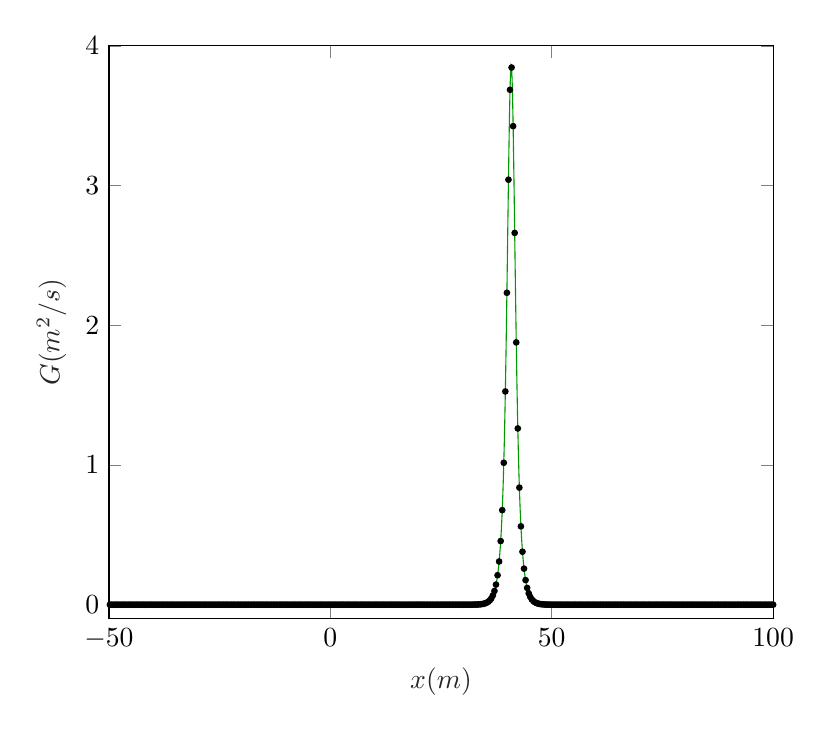
\begin{tikzpicture}

\begin{axis}[%
scale only axis,
xmin=-50,
xmax=100,
xtick={-50,   0,  50, 100},
xlabel style={font=\color{white!15!black}},
xlabel={$x (m)$},
ymin=-0.1,
ymax=4,
ytick={0, 1, 2, 3, 4},
ylabel style={font=\color{white!15!black}},
ylabel={$G (m^2/s)$},
axis background/.style={fill=white}
]
\addplot [color=green!60!black, forget plot]
  table[row sep=crcr]{%
-50.14064697609	-5.67925565028477e-44\\
-50.0234411626817	-6.46942449732437e-44\\
-49.9062353492733	-7.36953148507789e-44\\
-49.789029535865	-8.39487257823589e-44\\
-49.6718237224566	-9.56287190678446e-44\\
-49.5546179090483	-1.08933778628938e-43\\
-49.4374120956399	-1.2409000394494e-43\\
-49.3202062822316	-1.41354952273408e-43\\
-49.2030004688233	-1.61022015448423e-43\\
-49.0857946554149	-1.83425405633628e-43\\
-48.9685888420066	-2.08945834755365e-43\\
-48.8513830285982	-2.38016984129328e-43\\
-48.7341772151899	-2.71132874222405e-43\\
-48.6169714017815	-3.08856259787573e-43\\
-48.4997655883732	-3.51828193034678e-43\\
-48.3825597749648	-4.00778917348764e-43\\
-48.2653539615565	-4.56540276678192e-43\\
-48.1481481481481	-5.20059851471748e-43\\
-48.0309423347398	-5.92417061383291e-43\\
-47.9137365213315	-6.74841508385664e-43\\
-47.7965307079231	-7.68733872007089e-43\\
-47.6793248945148	-8.75689711773463e-43\\
-47.5621190811064	-9.97526581343133e-43\\
-47.4449132676981	-1.13631491509804e-42\\
-47.3277074542897	-1.29441321206272e-42\\
-47.2105016408814	-1.47450811504829e-42\\
-47.093295827473	-1.6796600661072e-42\\
-46.9760900140647	-1.91335531414344e-42\\
-46.8588842006564	-2.17956515847011e-42\\
-46.741678387248	-2.4828134350695e-42\\
-46.6244725738397	-2.82825339238234e-42\\
-46.5072667604313	-3.22175526301613e-42\\
-46.390060947023	-3.67000601952039e-42\\
-46.2728551336146	-4.18062300942952e-42\\
-46.1556493202063	-4.76228340062936e-42\\
-46.0384435067979	-5.42487163677648e-42\\
-45.9212376933896	-6.17964740855479e-42\\
-45.8040318799812	-7.03943699518549e-42\\
-45.6868260665729	-8.0188512277557e-42\\
-45.5696202531646	-9.13453377832024e-42\\
-45.4524144397562	-1.04054439940802e-41\\
-45.3352086263479	-1.18531790829781e-41\\
-45.2180028129395	-1.3502341125768e-41\\
-45.1007969995312	-1.53809551513841e-41\\
-44.9835911861228	-1.7520945380161e-41\\
-44.8663853727145	-1.99586777279541e-41\\
-44.7491795593061	-2.27355777901906e-41\\
-44.6319737458978	-2.58988348075698e-41\\
-44.5147679324894	-2.95022035762469e-41\\
-44.3975621190811	-3.36069179297554e-41\\
-44.2803563056728	-3.82827313159305e-41\\
-44.1631504922644	-4.36091021518543e-41\\
-44.0459446788561	-4.96765441001729e-41\\
-43.9287388654477	-5.65881642126743e-41\\
-43.8115330520394	-6.44614150795858e-41\\
-43.694327238631	-7.34300907597218e-41\\
-43.5771214252227	-8.36466004093106e-41\\
-43.4599156118143	-9.52845582464262e-41\\
-43.342709798406	-1.08541733863529e-40\\
-43.2255039849977	-1.23643413024305e-40\\
-43.1082981715893	-1.40846226056424e-40\\
-42.991092358181	-1.60442508898053e-40\\
-42.8738865447726	-1.827652709075e-40\\
-42.7566807313643	-2.081938538565e-40\\
-42.6394749179559	-2.3716037827318e-40\\
-42.5222691045476	-2.70157086680588e-40\\
-42.4050632911392	-3.07744708518192e-40\\
-42.2878574777309	-3.50561988895448e-40\\
-42.1706516643225	-3.99336543104426e-40\\
-42.0534458509142	-4.54897221347495e-40\\
-41.9362400375059	-5.18188193800127e-40\\
-41.8190342240975	-5.90284995363215e-40\\
-41.7018284106892	-6.72412802761265e-40\\
-41.5846225972808	-7.65967254578537e-40\\
-41.4674167838725	-8.72538168037957e-40\\
-41.3502109704641	-9.93936555554129e-40\\
-41.2330051570558	-1.13222540016589e-39\\
-41.1157993436474	-1.28975471283085e-39\\
-40.9985935302391	-1.46920146732771e-39\\
-40.8813877168308	-1.67361509139989e-39\\
-40.7641819034224	-1.90646928719458e-39\\
-40.6469760900141	-2.17172106160686e-39\\
-40.5297702766057	-2.47387796966146e-39\\
-40.4125644631974	-2.81807471363196e-39\\
-40.295358649789	-3.21016039958451e-39\\
-40.1781528363807	-3.65679793413976e-39\\
-40.0609470229723	-4.16557725055085e-39\\
-39.943741209564	-4.74514428820606e-39\\
-39.8265353961556	-5.40534791736657e-39\\
-39.7093295827473	-6.1574073059063e-39\\
-39.592123769339	-7.01410257219832e-39\\
-39.4749179559306	-7.98999196400849e-39\\
-39.3577121425223	-9.10165925402394e-39\\
-39.2405063291139	-1.03679955561304e-38\\
-39.1233005157056	-1.1810520351486e-38\\
-39.0060947022972	-1.3453747179742e-38\\
-38.8888888888889	-1.53256002097858e-38\\
-38.7716830754805	-1.74578887690003e-38\\
-38.6544772620722	-1.98868478949472e-38\\
-38.5372714486639	-2.26537540953428e-38\\
-38.4200656352555	-2.58056267802317e-38\\
-38.3028598218472	-2.93960272861585e-38\\
-38.1856540084388	-3.34859690705341e-38\\
-38.0684481950305	-3.81449545435936e-38\\
-37.9512423816221	-4.34521561573435e-38\\
-37.8340365682138	-4.94977618223231e-38\\
-37.7168307548054	-5.63845075155249e-38\\
-37.5996249413971	-6.42294231238227e-38\\
-37.4824191279887	-7.31658211909224e-38\\
-37.3652133145804	-8.3345562363561e-38\\
-37.2480075011721	-9.49416360348316e-38\\
-37.1308016877637	-1.08151100038787e-37\\
-37.0135958743554	-1.2319842935199e-37\\
-36.896390060947	-1.40339330708186e-37\\
-36.7791842475387	-1.59865087949707e-37\\
-36.6619784341303	-1.82107511958348e-37\\
-36.544772620722	-2.07444579282335e-37\\
-36.4275668073136	-2.36306855279352e-37\\
-36.3103609939053	-2.69184810927339e-37\\
-36.193155180497	-3.06637157641179e-37\\
-36.0759493670886	-3.49300341733039e-37\\
-35.9587435536803	-3.97899359860334e-37\\
-35.8415377402719	-4.53260079253712e-37\\
-35.7243319268636	-5.16323272088679e-37\\
-35.6071261134552	-5.88160602494042e-37\\
-35.4899203000469	-6.699928378722e-37\\
-35.3727144866385	-7.63210594005375e-37\\
-35.2555086732302	-8.69397966479689e-37\\
-35.1383028598218	-9.90359450007444e-37\\
-35.0210970464135	-1.12815060310125e-36\\
-34.9038912330052	-1.28511297919975e-36\\
-34.7866854195968	-1.46391391784721e-36\\
-34.6694796061885	-1.66759187211797e-36\\
-34.5522737927801	-1.89960804255711e-36\\
-34.4350679793718	-2.16390519507907e-36\\
-34.3178621659634	-2.46497466234507e-36\\
-34.2006563525551	-2.80793266720784e-36\\
-34.0834505391467	-3.19860726522513e-36\\
-33.9662447257384	-3.64363738370003e-36\\
-33.8490389123301	-4.15058564026676e-36\\
-33.7318330989217	-4.72806685820487e-36\\
-33.6146272855134	-5.38589446240624e-36\\
-33.497421472105	-6.13524724377348e-36\\
-33.3802156586967	-6.98885932596121e-36\\
-33.2630098452883	-7.96123656265768e-36\\
-33.14580403188	-9.06890304275518e-36\\
-33.0285982184716	-1.03306818923917e-35\\
-32.9113924050633	-1.17680151456735e-35\\
-32.7941865916549	-1.34053281198016e-35\\
-32.6769807782466	-1.52704444866057e-35\\
-32.5597749648383	-1.73950590940077e-35\\
-32.4425691514299	-1.98152765722979e-35\\
-32.3253633380216	-2.25722248780352e-35\\
-32.2081575246132	-2.57127542018214e-35\\
-32.0909517112049	-2.92902331168347e-35\\
-31.9737458977965	-3.33654554974806e-35\\
-31.8565400843882	-3.80076736198637e-35\\
-31.7393342709798	-4.32957750000788e-35\\
-31.6221284575715	-4.93196229689201e-35\\
-31.5049226441632	-5.61815837640502e-35\\
-31.3877168307548	-6.39982660902768e-35\\
-31.2705110173465	-7.29025027091278e-35\\
-31.1533052039381	-8.30456077318933e-35\\
-31.0360993905298	-9.45999479753952e-35\\
-30.9188935771214	-1.07761872076836e-34\\
-30.8016877637131	-1.22755047143627e-34\\
-30.6844819503047	-1.39834259639528e-34\\
-30.5672761368964	-1.59289745097464e-34\\
-30.450070323488	-1.81452120235933e-34\\
-30.3328645100797	-2.06698001292991e-34\\
-30.2156586966714	-2.3545640405285e-34\\
-30.098452883263	-2.68216034323976e-34\\
-29.9812470698547	-3.05533592759417e-34\\
-29.8640412564463	-3.48043235147226e-34\\
-29.746835443038	-3.96467348934472e-34\\
-29.6296296296296	-4.51628829115533e-34\\
-29.5124238162213	-5.14465062095144e-34\\
-29.3952180028129	-5.86043855160665e-34\\
-29.2780121894046	-6.67581582261175e-34\\
-29.1608063759962	-7.60463854453612e-34\\
-29.0436005625879	-8.66269066278986e-34\\
-28.9263947491796	-9.86795218204107e-34\\
-28.8091889357712	-1.12409047093557e-33\\
-28.6919831223629	-1.28048795083117e-33\\
-28.5747773089545	-1.45864539787368e-33\\
-28.4575714955462	-1.6615903299652e-33\\
-28.3403656821378	-1.89277149104129e-33\\
-28.2231598687295	-2.15611745728783e-33\\
-28.1059540553211	-2.45610339738575e-33\\
-27.9887482419128	-2.79782712127288e-33\\
-27.8715424285045	-3.18709570975801e-33\\
-27.7543366150961	-3.63052419712644e-33\\
-27.6371308016878	-4.13564798370029e-33\\
-27.5199249882794	-4.71105088863525e-33\\
-27.4027191748711	-5.36651101901884e-33\\
-27.2855133614627	-6.11316693409651e-33\\
-27.1683075480544	-6.96370692833562e-33\\
-27.051101734646	-7.93258464990982e-33\\
-26.9338959212377	-9.03626471871409e-33\\
-26.8166901078293	-1.02935025178213e-32\\
-26.699484294421	-1.17256629130129e-32\\
-26.5822784810127	-1.33570833165449e-32\\
-26.4650726676043	-1.52154872648717e-32\\
-26.347866854196	-1.73324555384564e-32\\
-26.2306610407876	-1.97439628296455e-32\\
-26.1134552273793	-2.24909890784659e-32\\
-25.9962494139709	-2.5620215865082e-32\\
-25.8790436005626	-2.91848196930506e-32\\
-25.7618377871542	-3.32453756440329e-32\\
-25.6446319737459	-3.78708867602171e-32\\
-25.5274261603376	-4.3139956647252e-32\\
-25.4102203469292	-4.91421252243247e-32\\
-25.2930145335209	-5.59793903204352e-32\\
-25.1758087201125	-6.37679409741217e-32\\
-25.0586029067042	-7.26401318914445e-32\\
-24.9413970932958	-8.27467326151825e-32\\
-24.8241912798875	-9.42594896264916e-32\\
-24.7069854664791	-1.07374044918077e-31\\
-24.5897796530708	-1.22313260635659e-31\\
-24.4725738396624	-1.39331006285001e-31\\
-24.3553680262541	-1.58716472862398e-31\\
-24.2381622128458	-1.80799087220775e-31\\
-24.1209563994374	-2.05954110183665e-31\\
-24.0037505860291	-2.34609013538603e-31\\
-23.8865447726207	-2.67250744277318e-31\\
-23.7693389592124	-3.04433999527589e-31\\
-23.652133145804	-3.46790652796809e-31\\
-23.5349273323957	-3.95040491712024e-31\\
-23.4177215189873	-4.50003449728256e-31\\
-23.300515705579	-5.12613539664557e-31\\
-23.1833098921707	-5.83934725847349e-31\\
-23.0661040787623	-6.65179004584142e-31\\
-22.948898265354	-7.5772700021819e-31\\
-22.8316924519456	-8.63151426763096e-31\\
-22.7144866385373	-9.83243813812407e-31\\
-22.5972808251289	-1.120044950891e-30\\
-22.4800750117206	-1.27587956760414e-30\\
-22.3628691983122	-1.45339583892122e-30\\
-22.2456633849039	-1.65561038692719e-30\\
-22.1284575714955	-1.88595954377831e-30\\
-22.0112517580872	-2.14835774699988e-30\\
-21.8940459446789	-2.44726405946538e-30\\
-21.7768401312705	-2.7877579444646e-30\\
-21.6596343178622	-3.17562558354374e-30\\
-21.5424285044538	-3.61745820395983e-30\\
-21.4252226910455	-4.12076408667597e-30\\
-21.3080168776371	-4.69409615830541e-30\\
-21.1908110642288	-5.34719733523786e-30\\
-21.0736052508204	-6.09116608985208e-30\\
-20.9563994374121	-6.93864505236433e-30\\
-20.8391936240038	-7.90403585331695e-30\\
-20.7219878105954	-9.0037438576331e-30\\
-20.6047819971871	-1.02564569491223e-29\\
-20.4875761837787	-1.16834631029645e-29\\
-20.3703703703704	-1.33090121428349e-29\\
-20.253164556962	-1.51607278301914e-29\\
-20.1359587435537	-1.72700772885597e-29\\
-20.0187529301453	-1.96729057399784e-29\\
-19.901547116737	-2.24100456406447e-29\\
-19.7843413033286	-2.55280105671022e-29\\
-19.6671354899203	-2.90797856445299e-29\\
-19.549929676512	-3.31257279492657e-29\\
-19.4327238631036	-3.77345921865547e-29\\
-19.3155180496953	-4.29846990733726e-29\\
-19.1983122362869	-4.89652662812327e-29\\
-19.0811064228786	-5.57779245563524e-29\\
-18.9639006094702	-6.35384447813479e-29\\
-18.8466947960619	-7.23787053272964e-29\\
-18.7294889826535	-8.24489331283325e-29\\
-18.6122831692452	-9.39202565624859e-29\\
-18.4950773558368	-1.06987613521126e-28\\
-18.3778715424285	-1.21873064085278e-28\\
-18.2606657290202	-1.38829564102781e-28\\
-18.1434599156118	-1.58145263792512e-28\\
-18.0262541022035	-1.80148404424055e-28\\
-17.9090482887951	-2.0521289628447e-28\\
-17.7918424753868	-2.3376467272134e-28\\
-17.6746366619784	-2.66288928239499e-28\\
-17.5574308485701	-3.03338363652019e-28\\
-17.4402250351617	-3.45542578399383e-28\\
-17.3230192217534	-3.93618769645192e-28\\
-17.2058134083451	-4.48383919963454e-28\\
-17.0886075949367	-5.10768680728865e-28\\
-16.9714017815284	-5.81833187137416e-28\\
-16.85419596812	-6.62785073609845e-28\\
-16.7369901547117	-7.54999995722585e-28\\
-16.6197843413033	-8.60045007405599e-28\\
-16.502578527895	-9.79705190667434e-28\\
-16.3853727144866	-1.11601399037952e-27\\
-16.2681669010783	-1.27128776961395e-27\\
-16.1509610876699	-1.44816517275059e-27\\
-16.0337552742616	-1.64965196527029e-27\\
-15.9165494608533	-1.87917211221926e-27\\
-15.7993436474449	-2.14062596334618e-27\\
-15.6821378340366	-2.4384565336808e-27\\
-15.5649320206282	-2.77772500589302e-27\\
-15.4477262072199	-3.16419673748154e-27\\
-15.3305203938115	-3.6044392343547e-27\\
-15.2133145804032	-4.10593375571712e-27\\
-15.0961087669948	-4.67720244681982e-27\\
-14.9789029535865	-5.32795316000339e-27\\
-14.8616971401782	-6.06924442504969e-27\\
-14.7444913267698	-6.91367337226614e-27\\
-14.6272855133615	-7.87558980177177e-27\\
-14.5100796999531	-8.97134003677153e-27\\
-14.3928738865448	-1.02195447047372e-26\\
-14.2756680731364	-1.16414151669705e-26\\
-14.1584622597281	-1.3261113973791e-26\\
-14.0412564463197	-1.51061654707431e-26\\
-13.9240506329114	-1.72079235334581e-26\\
-13.806844819503	-1.96021043796217e-26\\
-13.6896390060947	-2.23293935123833e-26\\
-13.5724331926864	-2.54361371092997e-26\\
-13.455227379278	-2.89751296059287e-26\\
-13.3380215658697	-3.30065108578702e-26\\
-13.2208157524613	-3.75987881271732e-26\\
-13.103609939053	-4.28300002602356e-26\\
-12.9864041256446	-4.87890438406459e-26\\
-12.8691983122363	-5.55771838529369e-26\\
-12.7519924988279	-6.33097745287205e-26\\
-12.6347866854196	-7.21182196183838e-26\\
-12.5175808720113	-8.21522054002271e-26\\
-12.4003750586029	-9.35822443736625e-26\\
-12.2831692451946	-1.06602572862732e-25\\
-12.1659634317862	-1.21434451770346e-25\\
-12.0487576183779	-1.38329926574592e-25\\
-11.9315518049695	-1.57576110462623e-25\\
-11.8143459915612	-1.79500063387508e-25\\
-11.6971401781528	-2.04474349960316e-25\\
-11.5799343647445	-2.32923370625412e-25\\
-11.4627285513361	-2.65330573707812e-25\\
-11.3455227379278	-3.0224667089047e-25\\
-11.2283169245195	-3.44298995731157e-25\\
-11.1111111111111	-3.9220216425292e-25\\
-10.9939052977028	-4.46770218768769e-25\\
-10.8766994842944	-5.08930461306618e-25\\
-10.7594936708861	-5.79739211712812e-25\\
-10.6422878574777	-6.60399758219424e-25\\
-10.5250820440694	-7.52282805518297e-25\\
-10.407876230661	-8.56949767825991e-25\\
-10.2906704172527	-9.76179302770403e-25\\
-10.1734646038444	-1.11199753700245e-24\\
-10.056258790436	-1.26671249717158e-24\\
-9.93905297702766	-1.44295333136797e-24\\
-9.82184716361932	-1.64371498754059e-24\\
-9.70464135021097	-1.87240910813395e-24\\
-9.58743553680262	-2.1329220058209e-24\\
-9.47022972339428	-2.42968070554245e-24\\
-9.35302390998594	-2.7677281751394e-24\\
-9.23581809657759	-3.15280902300708e-24\\
-9.11861228316924	-3.59146711907652e-24\\
-9.0014064697609	-4.09115679804335e-24\\
-8.88420065635255	-4.66036953457618e-24\\
-8.76699484294421	-5.30877824315931e-24\\
-8.64978902953587	-6.04740165472831e-24\\
-8.53258321612752	-6.88879156343276e-24\\
-8.41537740271917	-7.84724612550216e-24\\
-8.29817158931083	-8.93905283491006e-24\\
-8.18096577590249	-1.01827653048414e-23\\
-8.06375996249414	-1.15995185584475e-23\\
-7.94655414908579	-1.32133881867822e-23\\
-7.82934833567745	-1.50517994772675e-23\\
-7.7121425222691	-1.71459934652117e-23\\
-7.59493670886076	-1.95315578282238e-23\\
-7.47773089545242	-2.22490316452794e-23\\
-7.36052508204407	-2.53445942974058e-23\\
-7.24331926863572	-2.88708502168173e-23\\
-7.12611345522738	-3.28877228201366e-23\\
-7.00890764181904	-3.7463472816748e-23\\
-6.89170182841069	-4.26758581969034e-23\\
-6.77449601500234	-4.8613455611836e-23\\
-6.657290201594	-5.53771656007476e-23\\
-6.54008438818565	-6.30819272437408e-23\\
-6.42287857477731	-7.18586713786387e-23\\
-6.30567276136896	-8.18565455736856e-23\\
-6.18846694796062	-9.32454486661817e-23\\
-6.07126113455227	-1.06218917937732e-22\\
-5.95405532114393	-1.20997417989309e-22\\
-5.83684950773559	-1.37832087205614e-22\\
-5.71964369432724	-1.57009005474272e-22\\
-5.60243788091889	-1.78854055683312e-22\\
-5.48523206751055	-2.03738461610793e-22\\
-5.3680262541022	-2.32085096314685e-22\\
-5.25082044069386	-2.64375668224554e-22\\
-5.13361462728551	-3.0115890705196e-22\\
-5.01640881387717	-3.43059888626723e-22\\
-4.89920300046882	-3.90790657120676e-22\\
-4.78199718706048	-4.45162325167598e-22\\
-4.66479137365214	-5.07098857502693e-22\\
-4.54758556024379	-5.77652772353829e-22\\
-4.43037974683544	-6.58023027406032e-22\\
-4.31317393342709	-7.49575394284404e-22\\
-4.19596812001875	-8.53865667789042e-22\\
-4.07876230661041	-9.726661042881e-22\\
-3.96155649320206	-1.10799553854966e-21\\
-3.84435067979372	-1.26215369080274e-21\\
-3.72714486638537	-1.43776024702432e-21\\
-3.60993905297703	-1.637799376563e-21\\
-3.49273323956868	-1.86567044360962e-21\\
-3.37552742616034	-2.12524577427976e-21\\
-3.25832161275199	-2.42093646097287e-21\\
-3.14111579934364	-2.75776732225433e-21\\
-3.0239099859353	-3.14146229209073e-21\\
-2.90670417252696	-3.57854168950001e-21\\
-2.78949835911861	-4.07643302156808e-21\\
-2.67229254571027	-4.6435972027623e-21\\
-2.55508673230192	-5.28967233544967e-21\\
-2.43788091889358	-6.02563749495257e-21\\
-2.32067510548523	-6.86399930242403e-21\\
-2.20346929207689	-7.81900445606685e-21\\
-2.08626347866854	-8.90688183234557e-21\\
-1.96905766526019	-1.01461182713373e-20\\
-1.85185185185185	-1.15577727327786e-20\\
-1.73464603844351	-1.3165834161418e-20\\
-1.61744022503516	-1.4997629143058e-20\\
-1.50023441162681	-1.70842862787873e-20\\
-1.38302859821847	-1.94612651687457e-20\\
-1.26582278481013	-2.21689589947048e-20\\
-1.14861697140178	-2.52533809414499e-20\\
-1.03141115799344	-2.87669461216609e-20\\
-0.914205344585092	-3.2769362291932e-20\\
-0.796999531176745	-3.73286444963069e-20\\
-0.679793717768398	-4.2522270879673e-20\\
-0.562587904360058	-4.84384993123216e-20\\
-0.445382090951711	-5.51778671997359e-20\\
-0.328176277543363	-6.28548999646078e-20\\
-0.210970464135023	-7.16000572341759e-20\\
-0.0937646507266763	-8.15619498054077e-20\\
0.0234411626816708	-9.29098650620153e-20\\
0.140646976090011	-1.05836643758969e-19\\
0.257852789498358	-1.2056195706114e-19\\
0.375058602906705	-1.37336039524405e-19\\
0.492264416315052	-1.56443941455628e-19\\
0.609470229723392	-1.7821037291397e-19\\
0.726676043131739	-2.03005221670051e-19\\
0.843881856540087	-2.3124983889238e-19\\
0.961087669948427	-2.63424199376843e-19\\
1.07829348335677	-3.0007505799658e-19\\
1.19549929676512	-3.41825240978853e-19\\
1.31270511017347	-3.89384229900186e-19\\
1.42991092358181	-4.43560218258835e-19\\
1.54711673699016	-5.0527384550797e-19\\
1.6643225503985	-5.75573841938713e-19\\
1.78152836380684	-6.55654850274386e-19\\
1.89873417721519	-7.468777268271e-19\\
2.01593999062354	-8.50792667204355e-19\\
2.13314580403188	-9.69165549552229e-19\\
2.25035161744022	-1.10400794299894e-18\\
2.36755743084857	-1.25761129124728e-18\\
2.48476324425692	-1.43258585221445e-18\\
2.60196905766526	-1.63190505544009e-18\\
2.71917487107361	-1.85895603104999e-18\\
2.83638068448195	-2.11759716893897e-18\\
2.95358649789029	-2.41222368630501e-18\\
3.07079231129864	-2.74784231775607e-18\\
3.18799812470699	-3.13015639723567e-18\\
3.30520393811533	-3.56566277760675e-18\\
3.42240975152367	-4.06176223489603e-18\\
3.53961556493202	-4.62688523335374e-18\\
3.65682137834037	-5.27063518851562e-18\\
3.77402719174871	-6.00395166280868e-18\\
3.89123300515705	-6.83929626696383e-18\\
4.0084388185654	-7.79086442635072e-18\\
4.12564463197375	-8.87482661088508e-18\\
4.24285044538209	-1.01096031278477e-17\\
4.36005625879044	-1.15161771473073e-17\\
4.47726207219878	-1.31184512795408e-17\\
4.59446788560712	-1.49436537639508e-17\\
4.71167369901547	-1.70228011720496e-17\\
4.82887951242382	-1.93912254874488e-17\\
4.94608532583216	-2.20891745197898e-17\\
5.0632911392405	-2.51624958557439e-17\\
5.18049695264885	-2.86634159698041e-17\\
5.2977027660572	-3.26514277346808e-17\\
5.41490857946554	-3.71943014132084e-17\\
5.53211439287389	-4.23692363120529e-17\\
5.64932020628223	-4.82641726678348e-17\\
5.76652601969058	-5.49792860592091e-17\\
5.88373183309892	-6.262868974018e-17\\
6.00093764650727	-7.13423738232549e-17\\
6.11814345991561	-8.12684142659256e-17\\
6.23534927332395	-9.25754891988914e-17\\
6.3525550867323	-1.0545574535724e-16\\
6.46976090014065	-1.20128063325257e-16\\
6.58696671354899	-1.36841777082808e-16\\
6.70417252695734	-1.55880911061387e-16\\
6.82137834036568	-1.77569006712211e-16\\
6.93858415377403	7.04499652447659e-16\\
7.05578996718237	6.76356685553378e-16\\
7.17299578059072	6.44298118257833e-16\\
7.29020159399906	6.07779163419e-16\\
7.4074074074074	5.66179236316026e-16\\
7.52461322081575	5.187914087451e-16\\
7.6418190342241	4.6481039583772e-16\\
7.75902484763245	4.03318871455313e-16\\
7.87623066104079	1.2400461526653e-15\\
7.99343647444913	1.16025335006822e-15\\
8.11064228785748	1.06935877802938e-15\\
8.22784810126582	9.6581781998282e-16\\
8.34505391467417	1.75464522610409e-15\\
8.46225972808251	1.62028812064766e-15\\
8.57946554149086	1.46723757970471e-15\\
8.6966713548992	2.19966701254122e-15\\
8.81387716830755	2.00106514466603e-15\\
8.9310829817159	2.68160558209758e-15\\
9.04828879512424	3.33066954795203e-15\\
9.16549460853258	3.03710337004486e-15\\
9.28270042194093	3.60946687875131e-15\\
9.39990623534927	4.13530299295864e-15\\
9.51711204875762	5.51491251456027e-15\\
9.63431786216596	5.92737275627671e-15\\
9.75152367557431	6.27105786754127e-15\\
9.86872948898265	7.4431732678683e-15\\
9.985935302391	8.52604449246784e-15\\
10.1031411157993	9.50725477904178e-15\\
10.2203469292077	1.12794340635809e-14\\
10.337552742616	1.2919695799463e-14\\
10.4547585560244	1.44096859727564e-14\\
10.5719643694327	1.66352712033538e-14\\
10.6891701828411	1.8665860631684e-14\\
10.8063759962494	2.13810982838562e-14\\
10.9235818096578	2.38433049416946e-14\\
11.0407876230661	2.78308243249419e-14\\
11.1579934364744	3.14900049267945e-14\\
11.2751992498828	3.56819384357729e-14\\
11.3924050632911	4.03545863366771e-14\\
11.5096108766995	4.63554441403836e-14\\
11.6268166901078	5.27102112112611e-14\\
11.7440225035162	6.02487403504022e-14\\
11.8612283169245	6.88834078117178e-14\\
11.9784341303329	7.85143985411919e-14\\
12.0956399437412	8.90280099701405e-14\\
12.2128457571496	1.01201494084096e-13\\
12.3300515705579	1.15794082113248e-13\\
12.4472573839662	1.31730928714194e-13\\
12.5644631973746	1.49727352947061e-13\\
12.6816690107829	1.71378810509016e-13\\
12.7988748241913	1.94623316208983e-13\\
12.9160806375996	2.21898190617956e-13\\
13.033286451008	2.52881056686928e-13\\
13.1504922644163	2.88111458525937e-13\\
13.2676980778247	3.28077846606643e-13\\
13.384903891233	3.73210468978376e-13\\
13.5021097046413	4.2568682196768e-13\\
13.6193155180497	4.84888554293072e-13\\
13.736521331458	5.51924830480177e-13\\
13.8537271448664	6.28713586641477e-13\\
13.9709329582747	7.17061120847776e-13\\
14.0881387716831	8.15926237832966e-13\\
14.2053445850914	9.29563523903678e-13\\
14.3225503984998	1.05934222318704e-12\\
14.4397562119081	1.20644360089922e-12\\
14.5569620253165	1.37455511219495e-12\\
14.6741678387248	1.56621351223959e-12\\
14.7913736521331	1.78367769249551e-12\\
14.9085794655415	2.0316103436789e-12\\
15.0257852789498	2.31431359423626e-12\\
15.1429910923582	2.63658561869945e-12\\
15.2601969057665	3.00366349205996e-12\\
15.3774027191749	3.42115809333096e-12\\
15.4946085325832	3.89770027490109e-12\\
15.6118143459916	4.43941574627565e-12\\
15.7290201593999	5.05708304503515e-12\\
15.8462259728083	5.76058328019619e-12\\
15.9634317862166	6.56240236785392e-12\\
16.0806375996249	7.47567524890499e-12\\
16.1978434130333	8.51583741453226e-12\\
16.3150492264416	9.70044034047623e-12\\
16.43225503985	1.10498480164934e-11\\
16.5494608532583	1.25869974496629e-11\\
16.6666666666667	1.43389393944725e-11\\
16.783872480075	1.63338072536351e-11\\
16.9010782934834	1.86059037082805e-11\\
17.0182841068917	2.11943906731916e-11\\
17.1354899203	2.41437366925726e-11\\
17.2526957337084	2.75022868728026e-11\\
17.3699015471167	3.13289209766071e-11\\
17.4871073605251	3.56878405148137e-11\\
17.6043131739334	4.06532358790363e-11\\
17.7215189873418	4.63093119822287e-11\\
17.8387248007501	5.27529116277478e-11\\
17.9559306141585	6.00923721301736e-11\\
18.0731364275668	6.84534770491427e-11\\
18.1903422409752	7.79779725144793e-11\\
18.3075480543835	8.88264109953478e-11\\
18.4247538677918	1.01185293792682e-10\\
18.5419596812002	1.15263971149788e-10\\
18.6591654946085	1.31300304972158e-10\\
18.7763713080169	1.49568704282621e-10\\
18.8935771214252	1.70378696985551e-10\\
19.0107829348336	1.94083931884914e-10\\
19.1279887482419	2.21087039813816e-10\\
19.2451945616503	2.51847536584693e-10\\
19.3624003750586	2.86887245683508e-10\\
19.4796061884669	3.26803122464384e-10\\
19.5968120018753	3.72271959015278e-10\\
19.7140178152836	4.2406679836046e-10\\
19.831223628692	4.8306859894736e-10\\
19.9484294421003	5.50279340645031e-10\\
20.0656352555087	6.2684092820148e-10\\
20.182841068917	7.14054248834957e-10\\
20.3000468823254	8.134026869523e-10\\
20.4172526957337	9.26573485573149e-10\\
20.5344585091421	1.05548934970686e-09\\
20.6516643225504	1.20234269621174e-09\\
20.7688701359587	1.36962762750629e-09\\
20.8860759493671	1.56018732177038e-09\\
21.0032817627754	1.77726001323682e-09\\
21.1204875761838	2.02453477599012e-09\\
21.2376933895921	2.30621282957294e-09\\
21.3548992030005	2.62708178169132e-09\\
21.4721050164088	2.99259470439821e-09\\
21.5893108298172	3.40896123711507e-09\\
21.7065166432255	3.88325868200008e-09\\
21.8237224566338	4.42354642090899e-09\\
21.9409282700422	5.039004893022e-09\\
22.0581340834505	5.74009387675532e-09\\
22.1753398968589	6.53872731321492e-09\\
22.2925457102672	7.44847706538602e-09\\
22.4097515236756	8.48480229793672e-09\\
22.5269573370839	9.66531352227517e-09\\
22.6441631504923	1.10100718088318e-08\\
22.7613689639006	1.25419304879271e-08\\
22.878574777309	1.42869207246381e-08\\
22.9957805907173	1.62746953904763e-08\\
23.1129864041256	1.85390327705267e-08\\
23.230192217534	2.11184149675598e-08\\
23.3473980309423	2.40566719078874e-08\\
23.4646038443507	2.74037357635419e-08\\
23.581809657759	3.12164851421731e-08\\
23.6990154711674	3.55597115697239e-08\\
23.8162212845757	4.05072217045498e-08\\
23.9334270979841	4.61430921092188e-08\\
24.0506329113924	5.25630938509119e-08\\
24.1678387248007	5.98763261550833e-08\\
24.2850445382091	6.82070678624435e-08\\
24.4022503516174	7.76968853896477e-08\\
24.5194561650258	8.85070437070075e-08\\
24.6366619784341	1.00821247029413e-07\\
24.7538677918425	1.1484875460448e-07\\
24.8710736052508	1.30827945090361e-07\\
24.9882794186592	1.49030359311305e-07\\
25.1054852320675	1.69765320102649e-07\\
25.2226910454759	1.93385186342083e-07\\
25.3398968588842	2.20291342766761e-07\\
25.4571026722925	2.50941018476639e-07\\
25.5743084857009	2.85855058826503e-07\\
25.6915142991092	3.25626774548931e-07\\
25.8087201125176	3.70932027150908e-07\\
25.9259259259259	4.22540709487775e-07\\
26.0431317393343	4.81329833101205e-07\\
26.1603375527426	5.4829843077014e-07\\
26.277543366151	6.24584532254987e-07\\
26.3947491795593	7.1148450277315e-07\\
26.5119549929676	8.10475075926028e-07\\
26.629160806376	9.23238446084501e-07\\
26.7463666197843	1.05169085352027e-06\\
26.8635724331927	1.19801515152588e-06\\
26.980778246601	1.3646978958533e-06\\
27.0979840600094	1.55457160478368e-06\\
27.2151898734177	1.77086288830396e-06\\
27.3323956868261	2.01724728352007e-06\\
27.4496015002344	2.29791170841468e-06\\
27.5668073136428	2.61762561877808e-06\\
27.6840131270511	2.98182205022739e-06\\
27.8012189404594	3.39668994642382e-06\\
27.9184247538678	3.86927932937337e-06\\
28.0356305672761	4.40762109996003e-06\\
28.1528363806845	5.02086350780401e-06\\
28.2700421940928	5.71942760981789e-06\\
28.3872480075012	6.51518435488633e-06\\
28.5044538209095	7.42165630450217e-06\\
28.6216596343179	8.454247420254e-06\\
28.7388654477262	9.63050481972133e-06\\
28.8560712611346	1.09704169509731e-05\\
28.9732770745429	1.24967532438382e-05\\
29.0904828879512	1.42354510177999e-05\\
29.2076887013596	1.62160562181099e-05\\
29.3248945147679	1.84722254612266e-05\\
29.4421003281763	2.10422979253289e-05\\
29.5593061415846	2.39699467943057e-05\\
29.676511954993	2.73049213320218e-05\\
29.7937177684013	3.11038921735575e-05\\
29.9109235818097	3.543141420647e-05\\
30.028129395218	4.03610233869567e-05\\
30.1453352086263	4.59764861124935e-05\\
30.2625410220347	5.23732223738739e-05\\
30.379746835443	5.96599268373539e-05\\
30.4969526488514	6.79604153903211e-05\\
30.6141584622597	7.74157284720337e-05\\
30.7313642756681	8.81865268958671e-05\\
30.8485700890764	0.000100455820813016\\
30.9657759024848	0.000114432078097946\\
31.0829817158931	0.000130352764879346\\
31.2001875293015	0.000148488378236566\\
31.3173933427098	0.000169147039410214\\
31.4345991561181	0.000192679725343126\\
31.5518049695265	0.000219486227146894\\
31.6690107829348	0.000250021936355717\\
31.7862165963432	0.000284805573764508\\
31.9034224097515	0.000324427991524394\\
32.0206282231599	0.00036956219721324\\
32.1378340365682	0.00042097476908627\\
32.2550398499766	0.000479538855050475\\
32.3722456633849	0.000546248974354167\\
32.4894514767932	0.000622237871096495\\
32.6066572902016	0.000708795702770705\\
32.7238631036099	0.000807391885842149\\
32.8410689170183	0.000919699964270065\\
32.9582747304266	0.00104762591672266\\
33.075480543835	0.00119334037464924\\
33.1926863572433	0.00135931528724505\\
33.3098921706517	0.00154836564156118\\
33.42709798406	0.00176369692761302\\
33.5443037974684	0.00200895913045486\\
33.6615096108767	0.00228830813496124\\
33.778715424285	0.0026064755459206\\
33.8959212376934	0.00296884805739681\\
34.0131270511017	0.00338155765261079\\
34.1303328645101	0.0038515840807093\\
34.2475386779184	0.0043868712411525\\
34.3647444913268	0.00499645931221381\\
34.4819503047351	0.00569063468894814\\
34.5991561181435	0.00648110004999354\\
34.7163619315518	0.00738116715395361\\
34.8335677449601	0.00840597527687077\\
34.9507735583685	0.00957273854516631\\
35.0679793717768	0.0109010257960637\\
35.1851851851852	0.0124130770137129\\
35.3023909985935	0.0141341608487715\\
35.4195968120019	0.0160929782392172\\
35.5368026254102	0.0183221177212166\\
35.6540084388186	0.0208585686674843\\
35.7712142522269	0.0237442994420471\\
35.8884200656353	0.0270269083544166\\
36.0056258790436	0.0307603563934693\\
36.122831692452	0.035005792114396\\
36.2400375058603	0.0398324808794348\\
36.3572433192686	0.0453188531192728\\
36.474449132677	0.0515536896839815\\
36.5916549460853	0.058637467113298\\
36.7088607594937	0.0666838923661058\\
36.826066572902	0.0758216660114743\\
36.9432723863104	0.0861965261589085\\
37.0604781997187	0.0979736438396166\\
37.177684013127	0.111340465761539\\
37.2948898265354	0.126510134136342\\
37.4120956399437	0.143725657307186\\
37.5293014533521	0.163265060239153\\
37.6465072667604	0.18544780997582\\
37.7637130801688	0.210642884009107\\
37.8809188935771	0.239278919318419\\
37.9981247069855	0.271856927019288\\
38.1153305203938	0.308966047623336\\
38.2325363338022	0.351302699209388\\
38.3497421472105	0.399693152289034\\
38.4669479606189	0.455118936508369\\
38.5841537740272	0.518743403174827\\
38.7013595874355	0.591936081115553\\
38.8185654008439	0.676289050626706\\
38.9357712142522	0.773616410414419\\
39.0529770276606	0.885924245950563\\
39.1701828410689	1.01533493398509\\
39.2873886544773	1.16394729396258\\
39.4045944678856	1.33361480679152\\
39.5218002812939	1.5256301458044\\
39.6390060947023	1.74031788213731\\
39.7562119081106	1.97655972760745\\
39.873417721519	2.23130695402441\\
39.9906235349273	2.4991677259524\\
40.1078293483357	2.7721835271631\\
40.225035161744	3.03991577737864\\
40.3422409751524	3.28993855737342\\
40.4594467885607	3.5087697683505\\
40.5766526019691	3.6831771393487\\
40.6938584153774	3.80168867345452\\
40.8110642287858	3.85605242448379\\
40.9282700421941	3.84236156950501\\
41.0454758556024	3.76160713576826\\
41.1626816690108	3.61953661767913\\
41.2798874824191	3.42584992208795\\
41.3970932958275	3.1929075462474\\
41.5142991092358	2.93421649157851\\
41.6315049226442	2.66297480376634\\
41.7487107360525	2.39090093158618\\
41.8659165494608	2.12747622706502\\
41.9831223628692	1.87962296362839\\
42.1003281762775	1.65175555341958\\
42.2175339896859	1.44609450039702\\
42.3347398030942	1.2631215430121\\
42.4519456165026	1.10207080682944\\
42.5691514299109	0.961381300553836\\
42.6863572433193	0.83906894293178\\
42.8035630567276	0.733003824786157\\
42.920768870136	0.641097321765158\\
43.0379746835443	0.56141401545166\\
43.1551804969527	0.492226988879258\\
43.272386310361	0.432034306362408\\
43.3895921237693	0.379551484780163\\
43.5067979371777	0.333691047614705\\
43.624003750586	0.293536745663719\\
43.7412095639944	0.258317163049273\\
43.8584153774027	0.227381314611746\\
43.9756211908111	0.200177414040275\\
44.0928270042194	0.176235110326417\\
44.2100328176277	0.155151001248085\\
44.3272386310361	0.136577004334741\\
44.4444444444444	0.12021109647153\\
44.5616502578528	0.105789951555873\\
44.6788560712611	0.0930830650285291\\
44.7960618846695	0.0818880268273618\\
44.9132676980778	0.0720266752115634\\
45.0304735114862	0.0633419258984559\\
45.1476793248945	0.0556951217173727\\
45.2648851383029	0.0489637877354776\\
45.3820909517112	0.0430397069430314\\
45.4992967651196	0.0378272538771574\\
45.6165025785279	0.0332419397537066\\
45.7337083919362	0.0292091342818248\\
45.8509142053446	0.0256629375853651\\
45.9681200187529	0.0225451815022948\\
46.0853258321613	0.019804543690133\\
46.2025316455696	0.0173957609502312\\
46.319737458978	0.01527893036459\\
46.4369432723863	0.013418888472188\\
46.5541490857947	0.0117846599728802\\
46.671354899203	0.0103489684539457\\
46.7885607126113	0.00908780246542502\\
46.9057665260197	0.00798003097695619\\
47.022972339428	0.00700706286391573\\
47.1401781528364	0.00615254561573114\\
47.2573839662447	0.00540209894801401\\
47.3745897796531	0.00474307944168806\\
47.4917955930614	0.00416437273252394\\
47.6090014064698	0.00365621013788339\\
47.7262072198781	0.00321000693714024\\
47.8434130332865	0.0028182198210215\\
47.9606188466948	0.00247422129522856\\
48.0778246601031	0.00217218906745937\\
48.1950304735115	0.00190700866629904\\
48.3122362869198	0.00167418773745018\\
48.4294421003282	0.00146978063920566\\
48.5466479137365	0.00129032211684926\\
48.6638537271449	0.00113276897642273\\
48.7810595405532	0.000994448803638677\\
48.8982653539616	0.000873014885194374\\
49.0154711673699	0.000766406588715388\\
49.1326769807782	0.000672814545294697\\
49.2498827941866	0.000590650056332495\\
49.3670886075949	0.000518518215142778\\
49.4842944210033	0.000455194294565743\\
49.6015002344116	0.000399603005533313\\
49.71870604782	0.000350800278896128\\
49.8359118612283	0.000307957264620689\\
49.9531176746367	0.000270346279304261\\
50.070323488045	0.000237328465416525\\
50.1875293014534	0.00020834295424856\\
50.3047351148617	0.000182897349733278\\
50.42194092827	0.000160559372434788\\
50.5391467416784	0.000140949522488123\\
50.6563525550867	0.000123734637420259\\
50.7735583684951	0.000108622235832875\\
50.8907641819034	9.535555118558e-05\\
51.0079699953118	8.37091715792946e-05\\
51.1251758087201	7.34852116298702e-05\\
51.2423816221285	6.45099515715433e-05\\
51.3595874355368	5.66308865882875e-05\\
51.4767932489451	4.97141363256311e-05\\
51.5939990623535	4.36421706561349e-05\\
51.7112048757618	3.83118130820918e-05\\
51.8284106891702	3.36324879188859e-05\\
51.9456165025785	2.95246814844171e-05\\
52.0628223159869	2.59185911857115e-05\\
52.1800281293952	2.27529395618496e-05\\
52.2972339428036	1.99739331440549e-05\\
52.4144397562119	1.75343484536477e-05\\
52.5316455696203	1.53927296169867e-05\\
52.6488513830286	1.35126839663297e-05\\
52.7660571964369	1.18622636660737e-05\\
52.8832630098453	1.04134228530748e-05\\
53.0004688232536	9.14154108096375e-06\\
53.117674636662	8.02500495672601e-06\\
53.2348804500703	7.04484087936342e-06\\
53.3520862634787	6.18439262930557e-06\\
53.469292076887	5.42903832928282e-06\\
53.5864978902954	4.76594198592767e-06\\
53.7037037037037	4.18383536191298e-06\\
53.820909517112	3.67282649856413e-06\\
53.9381153305204	3.2242316211661e-06\\
54.0553211439287	2.83042757603355e-06\\
54.1725269573371	2.48472228533345e-06\\
54.2897327707454	2.18124103377709e-06\\
54.4069385841538	1.91482662996269e-06\\
54.5241443975621	1.68095177710319e-06\\
54.6413502109705	1.47564213539028e-06\\
54.7585560243788	1.29540878420287e-06\\
54.8757618377872	1.13718893501548e-06\\
54.9929676511955	9.98293884916949e-07\\
55.1101734646038	8.76363324924987e-07\\
55.2273792780122	7.69325232120056e-07\\
55.3445850914205	6.75360656522762e-07\\
55.4617909048289	5.92872813615988e-07\\
55.5789967182372	5.20459948363709e-07\\
55.6962025316456	4.56891513642067e-07\\
55.8134083450539	4.01087259981465e-07\\
55.9306141584623	3.52098879619226e-07\\
56.0478199718706	3.09093888214549e-07\\
56.165025785279	2.71341482066949e-07\\
56.2822315986873	2.38200114739226e-07\\
56.3994374120956	2.0910659940463e-07\\
56.516643225504	1.83566535170887e-07\\
56.6338490389123	1.61145909163934e-07\\
56.7510548523207	1.41463714063882e-07\\
56.868260665729	1.24185482935527e-07\\
56.9854664791374	1.09017595302862e-07\\
57.1026722925457	9.57022992092983e-08\\
57.2198781059541	8.40133195531076e-08\\
57.3370839193624	7.37520191109097e-08\\
57.4542897327707	6.47440233324812e-08\\
57.5714955461791	5.68362552085657e-08\\
57.6887013595874	4.98943338506582e-08\\
57.8059071729958	4.38002911038125e-08\\
57.9231129864041	3.84505689756135e-08\\
58.0403187998125	3.37542555331405e-08\\
58.1575246132208	2.96315457442955e-08\\
58.2747304266292	2.60123798993602e-08\\
58.3919362400375	2.28352544360361e-08\\
58.5091420534459	2.00461798853552e-08\\
58.6263478668542	1.75977598328886e-08\\
58.7435536802625	1.54483882075069e-08\\
58.8607594936709	1.35615373008148e-08\\
58.9779653070792	1.19051458347005e-08\\
59.0951711204876	1.0451063227664e-08\\
59.2123769338959	9.17458102442933e-09\\
59.3295827473043	8.05400685282222e-09\\
59.4467885607126	7.07029950451201e-09\\
59.563994374121	6.20673960097379e-09\\
59.6812001875293	5.4486551091703e-09\\
59.7984060009376	4.78316246774925e-09\\
59.915611814346	4.19895167988948e-09\\
60.0328176277543	3.68609621434977e-09\\
60.1500234411627	3.23588002627275e-09\\
60.267229254571	2.84065277233825e-09\\
60.3844350679794	2.49369866006619e-09\\
60.5016408813877	2.18912047782917e-09\\
60.6188466947961	1.92174379033749e-09\\
60.7360525082044	1.68702435595214e-09\\
60.8532583216128	1.48097250693703e-09\\
60.9704641350211	1.30008815693701e-09\\
61.0876699484294	1.1412963606888e-09\\
61.2048757618378	1.00189954894581e-09\\
61.3220815752461	8.79528924496902e-10\\
61.4392873886545	7.72103725720905e-10\\
61.5564932020628	6.77799743300379e-10\\
61.6736990154712	5.95013908843853e-10\\
61.7909048288795	5.22339832825461e-10\\
61.9081106422879	4.58541920950951e-10\\
62.0253164556962	4.02535607526243e-10\\
62.1425222691045	3.53370328379264e-10\\
62.2597280825129	3.10210011845675e-10\\
62.3769338959212	2.72321254724056e-10\\
62.4941397093296	2.39060284348352e-10\\
62.6113455227379	2.09861575362766e-10\\
62.7285513361463	1.84229158127154e-10\\
62.8457571495546	1.61728012687034e-10\\
62.962962962963	1.41974741835604e-10\\
63.0801687763713	1.24633958738684e-10\\
63.1973745897797	1.09411398676312e-10\\
63.314580403188	9.60483566279749e-11\\
63.4317862165964	8.43166034949625e-11\\
63.5489920300047	7.40183671234426e-11\\
63.666197843413	6.49778224194803e-11\\
63.7834036568214	5.70413595656553e-11\\
63.9006094702297	5.0074877650217e-11\\
64.0178152836381	4.39581347643837e-11\\
64.1350210970464	3.85897834444105e-11\\
64.2522269104548	3.38759121629375e-11\\
64.3694327238631	2.97383848501277e-11\\
64.4866385372714	2.61067259171765e-11\\
64.6038443506798	2.29180498783875e-11\\
64.7210501640881	2.01187023652085e-11\\
64.8382559774965	1.76612775896127e-11\\
64.9554617909048	1.55042774043464e-11\\
65.0726676043132	1.36107944784585e-11\\
65.1898734177215	1.19480415777351e-11\\
65.3070792311299	1.04886411344084e-11\\
65.4242850445382	9.20733419125833e-12\\
65.5414908579466	8.08308894762876e-12\\
65.6586966713549	7.09573262911721e-12\\
65.7759024847633	6.22889914723999e-12\\
65.8931082981716	5.46841512104384e-12\\
66.0103141115799	4.80066152342425e-12\\
66.1275199249883	4.21454102641495e-12\\
66.2447257383966	3.69979946481011e-12\\
66.361931551805	3.24714435808487e-12\\
66.4791373652133	2.85106927898996e-12\\
66.5963431786217	2.50269099709875e-12\\
66.71354899203	2.19708385482667e-12\\
66.8307548054383	1.92881628457429e-12\\
66.9479606188467	1.69291937432852e-12\\
67.065166432255	1.48675466040801e-12\\
67.1823722456634	1.30462110069318e-12\\
67.2995780590717	1.1450510715596e-12\\
67.4167838724801	1.00540641924392e-12\\
67.5339896858884	8.82817448986705e-13\\
67.6511954992968	7.75117979484482e-13\\
67.7684013127051	6.79963394683483e-13\\
67.8856071261135	5.9757276043556e-13\\
68.0028129395218	5.24400536546676e-13\\
68.1200187529302	4.60407566163365e-13\\
68.2372245663385	4.03635173987748e-13\\
68.3544303797468	3.54751980697062e-13\\
68.4716361931552	3.11624619508301e-13\\
68.5888420065635	2.7295480770559e-13\\
68.7060478199719	2.40101651354246e-13\\
68.8232536333802	2.10741912087993e-13\\
68.9404594467886	1.85224174873487e-13\\
69.0576652601969	1.6204090032236e-13\\
69.1748710736052	1.42367496221956e-13\\
69.2920768870136	1.25533011192667e-13\\
69.4092827004219	1.09930916416431e-13\\
69.5264885138303	9.66497207179167e-14\\
69.6436943272386	8.49421875046714e-14\\
69.760900140647	7.40415944161942e-14\\
69.8781059540553	6.49776618416961e-14\\
69.9953117674637	5.69515451122389e-14\\
70.112517580872	5.00579914212206e-14\\
70.2297233942804	4.43801756373891e-14\\
70.3469292076887	3.9084339463609e-14\\
70.4641350210971	3.42345807796795e-14\\
70.5813408345054	2.98871686163569e-14\\
70.6985466479137	2.60914993629177e-14\\
70.8157524613221	2.28909361845109e-14\\
70.9329582747304	2.03235459139431e-14\\
71.0501640881388	1.75159716672008e-14\\
71.1673699015471	1.54043235408897e-14\\
71.2845757149555	1.40143543112772e-14\\
71.4017815283638	1.15551227909443e-14\\
71.5189873417721	1.07667979182304e-14\\
71.6361931551805	8.94647900858701e-15\\
71.7533989685888	7.92300882115332e-15\\
71.8706047819972	6.80303927647333e-15\\
71.9878105954055	6.50513097973754e-15\\
72.1050164088139	5.2260821465019e-15\\
72.2222222222222	4.78852434172306e-15\\
72.3394280356306	4.29365692062473e-15\\
72.4566338490389	3.74847962073704e-15\\
72.5738396624473	3.15913723885505e-15\\
72.6910454758556	2.53102405262023e-15\\
72.8082512892639	2.77564976121125e-15\\
72.9254571026723	2.08362286457273e-15\\
73.0426629160806	2.27214121754178e-15\\
73.159868729489	1.53085985992756e-15\\
73.2770745428973	1.67613964107101e-15\\
73.3942803563057	8.96900826274584e-16\\
73.511486169714	1.0088592349742e-15\\
73.6286919831224	1.10714315891012e-15\\
73.7458977965307	1.19342278557182e-15\\
73.8631036099391	3.62390034414175e-16\\
73.9803094233474	4.28880564811534e-16\\
74.0975152367557	4.87250010286301e-16\\
74.2147210501641	5.38490271789258e-16\\
74.3319268635724	5.83472100510359e-16\\
74.4491326769808	6.2295989498576e-16\\
74.5663384903891	6.57624690901446e-16\\
74.6835443037975	6.88055564335636e-16\\
74.8007501172058	7.14769642220877e-16\\
74.9179559306142	-1.68553382915683e-16\\
75.0351617440225	-1.4796644627268e-16\\
75.1523675574308	-1.29893976874485e-16\\
75.2695733708392	-1.14028860280767e-16\\
75.3867791842475	-1.00101492692729e-16\\
75.5039849976559	-8.78751994419661e-17\\
75.6211908110642	-7.71422130603886e-17\\
75.7383966244726	-6.77201425845335e-17\\
75.8556024378809	-5.94488740954261e-17\\
75.9728082512893	-5.2187849823296e-17\\
76.0900140646976	-4.58136795796512e-17\\
76.207219878106	-4.02180439265778e-17\\
76.3244256915143	-3.53058534507796e-17\\
76.4416315049226	-3.09936328619949e-17\\
76.558837318331	-2.72081024559658e-17\\
76.6760431317393	-2.38849328360626e-17\\
76.7932489451477	-2.09676517319247e-17\\
76.910454758556	-1.84066843381488e-17\\
77.0276605719644	-1.61585108650196e-17\\
77.1448663853727	-1.41849269851291e-17\\
77.2620721987811	-1.24523946082822e-17\\
77.3792780121894	-1.09314719520895e-17\\
77.4964838255977	-9.59631322314836e-18\\
77.6136896390061	-8.42422940665085e-18\\
77.7308954524144	-7.39530270069679e-18\\
77.8481012658228	-6.49204804320211e-18\\
77.9653070792311	-5.69911597956279e-18\\
78.0825128926395	-5.00303182175574e-18\\
78.1997187060478	-4.39196666627946e-18\\
78.3169245194562	-3.85553637972687e-18\\
78.4341303328645	-3.38462513605323e-18\\
78.5513361462729	-2.97123050682107e-18\\
78.6685419596812	-2.60832747196311e-18\\
78.7857477730896	-2.28974904012956e-18\\
78.9029535864979	-2.01008144994479e-18\\
79.0201593999062	-1.76457217127315e-18\\
79.1373652133146	-1.54904914311669e-18\\
79.2545710267229	-1.35984987571195e-18\\
79.3717768401313	-1.19375921202419e-18\\
79.4889826535396	-1.04795469098865e-18\\
79.606188466948	-9.19958584028778e-19\\
79.7233942803563	-8.07595789785368e-19\\
79.8406000937647	-7.08956871539591e-19\\
79.957805907173	-6.22365609207544e-19\\
80.0750117205813	-5.46350514500436e-19\\
80.1922175339897	-4.79619825194007e-19\\
80.309423347398	-4.21039553572075e-19\\
80.4266291608064	-3.69614216010479e-19\\
80.5438349742147	-3.24469916229995e-19\\
80.6610407876231	-2.84839494743114e-19\\
80.7782466010314	-2.50049492132281e-19\\
80.8954524144397	-2.19508704619776e-19\\
81.0126582278481	-1.92698137448566e-19\\
81.1298640412564	-1.69162185346896e-19\\
81.2470698546648	-1.48500890201778e-19\\
81.3642756680731	-1.3036314437236e-19\\
81.4814814814815	-1.14440724143516e-19\\
81.5986872948898	-1.00463051927347e-19\\
81.7158931082982	-8.81925982039384e-20\\
81.8330989217065	-7.74208450643722e-20\\
81.9503047351149	-6.79647427624377e-20\\
82.0675105485232	-5.96635990594456e-20\\
82.1847163619315	-5.23763485012965e-20\\
82.3019221753399	-4.59791552232025e-20\\
82.4191279887482	-4.03633085454037e-20\\
82.5363338021566	-3.54333755986303e-20\\
82.6535396155649	-3.11055795860061e-20\\
82.7707454289733	-2.73063761223695e-20\\
82.8879512423816	-2.3971203458036e-20\\
83.00515705579	-2.10433853489569e-20\\
83.1223628691983	-1.84731679291733e-20\\
83.2395686826067	-1.62168742186896e-20\\
83.356774496015	-1.4236161898874e-20\\
83.4739803094234	-1.24973717424148e-20\\
83.5911861228317	-1.09709556253688e-20\\
83.70839193624	-9.63097440122639e-21\\
83.8255977496484	-8.45465710412654e-21\\
83.9428035630567	-7.42201399053168e-21\\
84.0600093764651	-6.51549684359919e-21\\
84.1772151898734	-5.71970076762278e-21\\
84.2944210032818	-5.0211024049966e-21\\
84.4116268166901	-4.40783012708925e-21\\
84.5288326300985	-3.86946229376662e-21\\
84.6460384435068	-3.39685015329059e-21\\
84.7632442569152	-2.98196237304021e-21\\
84.8804500703235	-2.61774855909201e-21\\
84.9976558837318	-2.29801944537679e-21\\
85.1148616971402	-2.01734171641044e-21\\
85.2320675105485	-1.77094567626807e-21\\
85.3492733239569	-1.55464419477379e-21\\
85.4664791373652	-1.36476155352044e-21\\
85.5836849507735	-1.19807098256237e-21\\
85.7008907641819	-1.05173982631276e-21\\
85.8180965775902	-9.23281406821685e-22\\
85.9353023909986	-8.10512766423574e-22\\
86.0525082044069	-7.1151757165461e-22\\
86.1697140178153	-6.24613548047051e-22\\
86.2869198312236	-5.48323892404617e-22\\
86.404125644632	-4.8135217675282e-22\\
86.5213314580403	-4.22560317495147e-22\\
86.6385372714487	-3.70949235393812e-22\\
86.755743084857	-3.25641877720402e-22\\
86.8729488982653	-2.85868314063768e-22\\
86.9901547116737	-2.50952652520401e-22\\
87.107360525082	-2.20301553928005e-22\\
87.2245663384904	-1.93394148958628e-22\\
87.3417721518987	-1.69773186727743e-22\\
87.4589779653071	-1.49037264503074e-22\\
87.5761837787154	-1.30834006468754e-22\\
87.6933895921238	-1.14854075628269e-22\\
87.8105954055321	-1.00825917087346e-22\\
87.9278012189405	-8.85111433869097e-23\\
88.0450070323488	-7.77004834666783e-23\\
88.1622128457572	-6.82102264182061e-23\\
88.2794186591655	-5.9879099594256e-23\\
88.3966244725738	-5.25655280226675e-23\\
88.5138302859822	-4.61452285526183e-23\\
88.6310360993905	-4.05090978493563e-23\\
88.7482419127989	-3.55613583471058e-23\\
88.8654477262072	-3.12179306533576e-23\\
88.9826535396156	-2.7405004746033e-23\\
89.0998593530239	-2.40577856831563e-23\\
89.2170651664323	-2.11193925102473e-23\\
89.3342709798406	-1.8539891654043e-23\\
89.451476793249	-1.62754483765033e-23\\
89.5686826066573	-1.42875818693617e-23\\
89.6858884200656	-1.25425113306506e-23\\
89.803094233474	-1.10105819107739e-23\\
89.9203000468823	-9.66576077293256e-24\\
90.0375058602907	-8.48519470420903e-24\\
90.154711673699	-7.44882175958256e-24\\
90.2719174871074	-6.53903033933984e-24\\
90.3891233005157	-5.74035990642428e-24\\
90.506329113924	-5.03923825785614e-24\\
90.6235349273324	-4.42375088555351e-24\\
90.7407407407407	-3.88343850718452e-24\\
90.8579465541491	-3.40911932639174e-24\\
90.9751523675574	-2.99273300197151e-24\\
91.0923581809658	-2.62720367449522e-24\\
91.2095639943741	-2.30631972271985e-24\\
91.3267698077825	-2.02462820642504e-24\\
91.4439756211908	-1.77734220189457e-24\\
91.5611814345991	-1.56025945534631e-24\\
91.6783872480075	-1.36969097194819e-24\\
91.7955930614158	-1.20239832689879e-24\\
91.9127988748242	-1.05553863326746e-24\\
92.0300046882325	-9.26616231406276e-25\\
92.1472105016409	-8.13440278967041e-25\\
92.2644163150492	-7.1408752083023e-25\\
92.3816221284576	-6.26869606276451e-25\\
92.4988279418659	-5.5030439800475e-25\\
92.6160337552743	-4.83090785438126e-25\\
92.7332395686826	-4.24086574305739e-25\\
92.850445382091	-3.72289076769027e-25\\
92.9676511954993	-3.2681807224959e-25\\
93.0848570089076	-2.86900849404188e-25\\
93.202062822316	-2.5185907505747e-25\\
93.3192686357243	-2.21097266949662e-25\\
93.4364744491327	-1.94092674411105e-25\\
93.553680262541	-1.70386395000671e-25\\
93.6708860759494	-1.4957557614892e-25\\
93.7880918893577	-1.31306569284438e-25\\
93.9052977027661	-1.15268920108203e-25\\
94.0225035161744	-1.01190092889637e-25\\
94.1397093295828	-8.88308391316697e-26\\
94.2569151429911	-7.79811319023397e-26\\
94.3741209563995	-6.84565967428972e-26\\
94.4913267698078	-6.00953785011578e-26\\
94.6085325832161	-5.27553908465677e-26\\
94.7257383966245	-4.63119017266927e-26\\
94.8429442100328	-4.06554137335608e-26\\
94.9601500234412	-3.56898033598629e-26\\
95.0773558368495	-3.13306875245064e-26\\
95.1945616502579	-2.75039896090365e-26\\
95.3117674636662	-2.41446806369096e-26\\
95.4289732770745	-2.11956742038189e-26\\
95.5461790904829	-1.86068563801024e-26\\
95.6633849038912	-1.63342340998708e-26\\
95.7805907172996	-1.43391875650037e-26\\
95.8977965307079	-1.25878139597612e-26\\
96.0150023441163	-1.10503513234095e-26\\
96.1322081575246	-9.70067279045635e-27\\
96.2494139709329	-8.51584260385896e-27\\
96.3666197843413	-7.47572635632474e-27\\
96.4838255977496	-6.56264883633774e-27\\
96.601031411158	-5.76109366451678e-27\\
96.7182372245663	-5.05743961608316e-27\\
96.8354430379747	-4.4397291486272e-27\\
96.952648851383	-3.89746520165797e-27\\
97.0698546647914	-3.42143281484452e-27\\
97.1870604781997	-3.0035425336228e-27\\
97.3042662916081	-2.63669294108046e-27\\
97.4214721050164	-2.31464998005464e-27\\
97.5386779184248	-2.03194101470598e-27\\
97.6558837318331	-1.78376183130156e-27\\
97.7730895452414	-1.56589499782728e-27\\
97.8902953586498	-1.37463819507306e-27\\
98.0075011720581	-1.20674130128492e-27\\
98.1247069854665	-1.05935116123372e-27\\
98.2419127988748	-9.29963101132172e-28\\
98.3591186122832	-8.16378365470628e-28\\
98.4763244256915	-7.16666752473414e-28\\
98.5935302390999	-6.29133813222348e-28\\
98.7107360525082	-5.52292057045569e-28\\
98.8279418659166	-4.84835673850223e-28\\
98.9451476793249	-4.25618343843774e-28\\
99.0623534927333	-3.7363375755282e-28\\
99.1795593061416	-3.27998515106964e-28\\
99.2967651195499	-2.87937114186382e-28\\
99.4139709329583	-2.52768771526118e-28\\
99.5311767463666	-2.2189585402828e-28\\
99.648382559775	-1.94793722886178e-28\\
99.7655883731833	-1.71001818136819e-28\\
99.8827941865917	-1.50115832136868e-28\\
100	-1.31780838962278e-28\\
100.117205813408	-1.15685262975915e-28\\
};
\addplot [color=black, draw=none, mark=*, mark options={solid, black}, forget plot, mark size = 1pt]
  table[row sep=crcr]{%
-50.14064697609	-2.95400040009622e-24\\
-49.789029535865	1.03646958237348e-10\\
-49.4374120956399	2.36656884481641e-10\\
-49.0857946554149	3.86337385683654e-10\\
-48.7341772151899	5.66359727425905e-10\\
-48.3825597749648	7.90215418995016e-10\\
-48.0309423347398	1.07446634423089e-09\\
-47.6793248945148	1.43964566354327e-09\\
-47.3277074542897	1.91158516136956e-09\\
-46.9760900140647	2.52281615995698e-09\\
-46.6244725738397	3.31460615928257e-09\\
-46.2728551336146	4.33911129092062e-09\\
-45.9212376933896	5.66214856683361e-09\\
-45.5696202531646	7.36671216480949e-09\\
-45.2180028129395	9.55691827987737e-09\\
-44.8663853727145	1.2363074947823e-08\\
-44.5147679324894	1.59473605715877e-08\\
-44.1631504922644	2.05111082379537e-08\\
-43.8115330520394	2.6302917043685e-08\\
-43.4599156118143	3.36282430128134e-08\\
-43.1082981715893	4.28606275578932e-08\\
-42.7566807313643	5.44544951930585e-08\\
-42.4050632911392	6.8959465908645e-08\\
-42.0534458509142	8.70364988742456e-08\\
-41.7018284106892	1.09475390838716e-07\\
-41.3502109704641	1.37213709535671e-07\\
-40.9985935302391	1.71356517777445e-07\\
-40.6469760900141	2.13196333907376e-07\\
-40.295358649789	2.64232492955689e-07\\
-39.943741209564	3.26188703653321e-07\\
-39.592123769339	4.01027113029937e-07\\
-39.2405063291139	4.90957041939192e-07\\
-38.8888888888889	5.9843588340522e-07\\
-38.5372714486639	7.26159227879617e-07\\
-38.1856540084388	8.77036930642615e-07\\
-37.8340365682138	1.05415121640663e-06\\
-37.4824191279887	1.26069282380109e-06\\
-37.1308016877637	1.49987091147339e-06\\
-36.7791842475387	1.77479264850261e-06\\
-36.4275668073136	2.08830880374132e-06\\
-36.0759493670886	2.44282277198724e-06\\
-35.7243319268636	2.84006169762107e-06\\
-35.3727144866385	3.2808112418537e-06\\
-35.0210970464135	3.76461760545556e-06\\
-34.6694796061885	4.289465402538e-06\\
-34.3178621659634	4.85144416803823e-06\\
-33.9662447257384	5.4444219185822e-06\\
-33.6146272855134	6.05975101927344e-06\\
-33.2630098452883	6.68603734550981e-06\\
-32.9113924050633	7.30901072523332e-06\\
-32.5597749648383	7.91153984559407e-06\\
-32.2081575246132	8.4738383660172e-06\\
-31.8565400843882	8.97390957565523e-06\\
-31.5049226441632	9.38827355827672e-06\\
-31.1533052039381	9.69301147640544e-06\\
-30.8016877637131	9.86514485230625e-06\\
-30.450070323488	9.88434291857014e-06\\
-30.098452883263	9.73492605798479e-06\\
-29.746835443038	9.40807931098156e-06\\
-29.3952180028129	8.90413561264857e-06\\
-29.0436005625879	8.23477653869724e-06\\
-28.6919831223629	7.42488973094829e-06\\
-28.3403656821378	6.51380911387594e-06\\
-27.9887482419128	5.55562102725339e-06\\
-27.6371308016878	4.61821055256423e-06\\
-27.2855133614627	3.78074720258621e-06\\
-26.9338959212377	3.12938147840692e-06\\
-26.5822784810127	2.75104401205556e-06\\
-26.2306610407876	2.72545879024131e-06\\
-25.8790436005626	3.11558965338134e-06\\
-25.5274261603376	3.95730320311374e-06\\
-25.1758087201125	5.24906613616965e-06\\
-24.8241912798875	6.94285685131256e-06\\
-24.4725738396624	8.93795597399974e-06\\
-24.1209563994374	1.10790745584338e-05\\
-23.7693389592124	1.31604786599303e-05\\
-23.4177215189873	1.49373597634706e-05\\
-23.0661040787623	1.61451445761812e-05\\
-22.7144866385373	1.65259283903674e-05\\
-22.3628691983122	1.58647166784525e-05\\
-22.0112517580872	1.40205978943223e-05\\
-21.6596343178622	1.09681544595077e-05\\
-21.3080168776371	6.82461212697492e-06\\
-20.9563994374121	1.86744247840439e-06\\
-20.6047819971871	-3.46765924391311e-06\\
-20.253164556962	-8.61266383294905e-06\\
-19.901547116737	-1.29197258869112e-05\\
-19.549929676512	-1.57395444490595e-05\\
-19.1983122362869	-1.65178561882513e-05\\
-18.8466947960619	-1.49056513300164e-05\\
-18.4950773558368	-1.08465963647996e-05\\
-18.1434599156118	-4.65407685142382e-06\\
-17.7918424753868	2.97473917115504e-06\\
-17.4402250351617	1.10052826351936e-05\\
-17.0886075949367	1.81864136842929e-05\\
-16.7369901547117	2.32397000394805e-05\\
-16.3853727144866	2.50914703390271e-05\\
-16.0337552742616	2.3131748383745e-05\\
-15.6821378340366	1.7381735582233e-05\\
-15.3305203938115	8.62304121199904e-06\\
-14.9789029535865	-1.66534397863718e-06\\
-14.6272855133615	-1.15224468808547e-05\\
-14.2756680731364	-1.88784071710369e-05\\
-13.9240506329114	-2.20364903003484e-05\\
-13.5724331926864	-2.0062871025959e-05\\
-13.2208157524613	-1.32543539488025e-05\\
-12.8691983122363	-3.06844908701854e-06\\
-12.5175808720113	8.05987704243422e-06\\
-12.1659634317862	1.73000927643804e-05\\
-11.8143459915612	2.21907898264292e-05\\
-11.4627285513361	2.13938193114194e-05\\
-11.1111111111111	1.51833572229207e-05\\
-10.7594936708861	5.4653123314907e-06\\
-10.407876230661	-4.75475165491287e-06\\
-10.056258790436	-1.23325403139999e-05\\
-9.70464135021097	-1.50649696754613e-05\\
-9.35302390998594	-1.24672148286728e-05\\
-9.0014064697609	-5.9321406085518e-06\\
-8.64978902953587	1.88533384312976e-06\\
-8.29817158931083	8.16928984384194e-06\\
-7.94655414908579	1.1060569482807e-05\\
-7.59493670886076	1.02505274313234e-05\\
-7.24331926863572	6.79248408507199e-06\\
-6.89170182841069	2.3369540307206e-06\\
-6.54008438818565	-1.67860801652148e-06\\
-6.18846694796062	-4.37323721059083e-06\\
-5.83684950773559	-5.26862475669651e-06\\
-5.48523206751055	-4.10667179898062e-06\\
-5.13361462728551	-1.034797790933e-06\\
-4.78199718706048	2.8918773658184e-06\\
-4.43037974683544	5.77859238508551e-06\\
-4.07876230661041	5.97512184113059e-06\\
-3.72714486638537	3.45105490947308e-06\\
-3.37552742616034	-1.52712806744342e-09\\
-3.0239099859353	-2.22626607168081e-06\\
-2.67229254571027	-2.30104828195146e-06\\
-2.32067510548523	-8.99134547997052e-07\\
-1.96905766526019	7.706121316029e-07\\
-1.61744022503516	2.07947036386286e-06\\
-1.26582278481013	2.96585824379571e-06\\
-0.914205344585092	2.97753371539827e-06\\
-0.562587904360058	7.56465603820452e-07\\
-0.210970464135023	-2.8733000484796e-06\\
0.140646976090011	-8.39463728890878e-07\\
0.492264416315052	9.69384098393194e-06\\
0.843881856540087	-2.12615695354835e-05\\
1.19549929676512	2.74056742186561e-05\\
1.54711673699016	-2.80581720531591e-05\\
1.89873417721519	1.90073281258153e-05\\
2.25035161744022	2.0065804459241e-05\\
2.60196905766526	-2.75891750078342e-05\\
2.95358649789029	-8.04428039373917e-06\\
3.30520393811533	1.46334170058194e-05\\
3.65682137834037	9.44136054564903e-06\\
4.0084388185654	-3.93196198773796e-06\\
4.36005625879044	-4.77372105810087e-06\\
4.71167369901547	4.41750420981633e-06\\
5.0632911392405	9.22071802527479e-06\\
5.41490857946554	2.07372023333238e-06\\
5.76652601969058	-1.08231899351023e-05\\
6.11814345991561	-1.73745728178371e-05\\
6.46976090014065	-9.97937181796112e-06\\
6.82137834036568	8.63658113207239e-06\\
7.17299578059072	2.73127898131711e-05\\
7.52461322081575	3.31244520116775e-05\\
7.87623066104079	1.93670110078828e-05\\
8.22784810126582	-9.49607352010866e-06\\
8.57946554149086	-3.92108737868049e-05\\
8.9310829817159	-5.29766725608875e-05\\
9.28270042194093	-4.08622623130016e-05\\
9.63431786216596	-5.50283544048377e-06\\
9.985935302391	3.83803487451055e-05\\
10.337552742616	7.09870397020787e-05\\
10.6891701828411	7.66781010955842e-05\\
11.0407876230661	5.1043852850292e-05\\
11.3924050632911	2.62613477159092e-06\\
11.7440225035162	-5.08582630632839e-05\\
12.0956399437412	-8.97545029552626e-05\\
12.4472573839662	-9.98781387660579e-05\\
12.7988748241913	-7.70749356792701e-05\\
13.1504922644163	-2.83337061281286e-05\\
13.5021097046413	3.15318181242458e-05\\
13.8537271448664	8.48659904534348e-05\\
14.2053445850914	0.000116637640662201\\
14.5569620253165	0.000118463421983687\\
14.9085794655415	9.02805568221747e-05\\
15.2601969057665	3.96007150857756e-05\\
15.6118143459916	-2.11026644395078e-05\\
15.9634317862166	-7.78510133676131e-05\\
16.3150492264416	-0.000118495649297633\\
16.6666666666667	-0.000135142808806798\\
17.0182841068917	-0.000125415887143853\\
17.3699015471167	-9.21207415981371e-05\\
17.7215189873418	-4.22717310882902e-05\\
18.0731364275668	1.47871750545399e-05\\
18.4247538677918	6.93002655304343e-05\\
18.7763713080169	0.000112794627020279\\
19.1279887482419	0.000139291891094499\\
19.4796061884669	0.000145953263128513\\
19.831223628692	0.000132853069786013\\
20.182841068917	0.000102991451437853\\
20.5344585091421	6.10652324937997e-05\\
20.8860759493671	1.28003608582e-05\\
21.2376933895921	-3.59646466921607e-05\\
21.5893108298172	-7.99926308046821e-05\\
21.9409282700422	-0.000115164225663314\\
22.2925457102672	-0.000138754713957231\\
22.6441631504923	-0.000149506919780926\\
22.9957805907173	-0.000147508512223507\\
23.3473980309423	-0.000133960316391886\\
23.6990154711674	-0.000110870662975469\\
24.0506329113924	-8.07291159521446e-05\\
24.4022503516174	-4.62020349911721e-05\\
24.7538677918425	-9.87457768065478e-06\\
25.1054852320675	2.5945553169372e-05\\
25.4571026722925	5.93582176280017e-05\\
25.8087201125176	8.89385111590516e-05\\
26.1603375527426	0.000113750906187527\\
26.5119549929676	0.000133323205293807\\
26.8635724331927	0.000147591399241642\\
27.2151898734177	0.000156829709462326\\
27.5668073136428	0.000161592513391626\\
27.9184247538678	0.000162614998996978\\
28.2700421940928	0.000160794695319979\\
28.6216596343179	0.000157148978311498\\
28.9732770745429	0.000152808555967132\\
29.3248945147679	0.000149053344917001\\
29.676511954993	0.000147380220660074\\
30.028129395218	0.000149642267342414\\
30.379746835443	0.000158253536106007\\
30.7313642756681	0.000176501787124926\\
31.0829817158931	0.000209020835727105\\
31.4345991561181	0.000262482592781509\\
31.7862165963432	0.000346617377555197\\
32.1378340365682	0.000475716154940641\\
32.4894514767932	0.000670843386829772\\
32.8410689170183	0.000963098223005656\\
33.1926863572433	0.00139842163849031\\
33.5443037974684	0.00204468090004107\\
33.8959212376934	0.00300210304352312\\
34.2475386779184	0.00441862111356176\\
34.5991561181435	0.0065124016474856\\
34.9507735583685	0.00960481788007161\\
35.3023909985935	0.0141685169720342\\
35.6540084388186	0.0208971173101822\\
36.0056258790436	0.0308056256483223\\
36.3572433192686	0.0453742421566508\\
36.7088607594937	0.0667539892986881\\
37.0604781997187	0.0980645440190278\\
37.4120956399437	0.143845074278216\\
37.7637130801688	0.210799546953203\\
38.1153305203938	0.309167615407645\\
38.4669479606189	0.455368700263557\\
38.8185654008439	0.676587687241612\\
39.1701828410689	1.01570729190161\\
39.5218002812939	1.52619807407908\\
39.873417721519	2.23234347644956\\
40.225035161744	3.04163369986331\\
40.5766526019691	3.68515627019227\\
40.9282700421941	3.84458361720826\\
41.2798874824191	3.42505544982885\\
41.6315049226442	2.66079447825341\\
41.9831223628692	1.8772169437669\\
42.3347398030942	1.26123825753106\\
42.6863572433193	0.837830263802349\\
43.0379746835443	0.560653857471601\\
43.3895921237693	0.379085679202422\\
43.7412095639944	0.25802333986942\\
44.0928270042194	0.176044114902144\\
44.4444444444444	0.120084575726433\\
44.7960618846695	0.0818035382313421\\
45.1476793248945	0.0556386191839446\\
45.4992967651196	0.0377895264435189\\
45.8509142053446	0.0256378105996543\\
46.2025316455696	0.0173790693039359\\
46.5541490857947	0.0117735972466411\\
46.9057665260197	0.00797271310181035\\
47.2573839662447	0.00539726608849524\\
47.6090014064698	0.00365302282670018\\
47.9606188466948	0.00247212177630868\\
48.3122362869198	0.00167280627734023\\
48.6638537271449	0.00113186092943377\\
49.0154711673699	0.000765810319009331\\
49.3670886075949	0.000518127065265753\\
49.71870604782	0.00035054394695426\\
50.070323488045	0.000237160659453301\\
50.42194092827	0.000160449639296839\\
50.7735583684951	0.000108550560522079\\
51.1251758087201	7.34384517207494e-05\\
51.4767932489451	4.9683670193293e-05\\
51.8284106891702	3.36126652193379e-05\\
52.1800281293952	2.27400609726196e-05\\
52.5316455696203	1.53843758461e-05\\
52.8832630098453	1.04080133521052e-05\\
53.2348804500703	7.04134446786104e-06\\
53.5864978902954	4.76368658610016e-06\\
53.9381153305204	3.22277998762383e-06\\
54.2897327707454	2.18030891061666e-06\\
54.6413502109705	1.47504519524529e-06\\
54.9929676511955	9.97912718439207e-07\\
55.3445850914205	6.75118055774059e-07\\
55.6962025316456	4.56737672087775e-07\\
56.0478199718706	3.08996746864536e-07\\
56.3994374120956	2.09045518369605e-07\\
56.7510548523207	1.414255231379e-07\\
57.1026722925457	9.56785886463346e-08\\
57.4542897327707	6.47294221037e-08\\
57.8059071729958	4.37913587343895e-08\\
58.1575246132208	2.96261305716674e-08\\
58.5091420534459	2.00429567805479e-08\\
58.8607594936709	1.35596553551269e-08\\
59.2123769338959	9.1735226772051e-09\\
59.563994374121	6.20613978183313e-09\\
59.915611814346	4.19862880954706e-09\\
60.267229254571	2.8404687519739e-09\\
60.6188466947961	1.92169370719034e-09\\
60.9704641350211	1.30007843859085e-09\\
61.3220815752461	8.79528471003128e-10\\
61.6736990154712	5.9501905773618e-10\\
62.0253164556962	4.02551773308475e-10\\
62.3769338959212	2.72341390973217e-10\\
62.7285513361463	1.84240579321171e-10\\
63.0801687763713	1.24644407519059e-10\\
63.4317862165964	8.43293005483623e-11\\
63.7834036568214	5.70415227378207e-11\\
64.1350210970464	3.85860536707547e-11\\
64.4866385372714	2.61008751537986e-11\\
64.8382559774965	1.7650263082197e-11\\
65.1898734177215	1.19328601703899e-11\\
65.5414908579466	8.06483744383168e-12\\
65.8931082981716	5.44929090482558e-12\\
66.2447257383966	3.67695689964009e-12\\
66.5963431786217	2.47890783011448e-12\\
66.9479606188467	1.67005887131158e-12\\
67.2995780590717	1.12410213594321e-12\\
67.6511954992968	7.5110510331428e-13\\
68.0028129395218	4.99631156388803e-13\\
68.3544303797468	3.28357008753073e-13\\
68.7060478199719	2.12108079341901e-13\\
69.0576652601969	1.34137562608682e-13\\
69.4092827004219	8.04172902708719e-14\\
69.760900140647	4.87723525172224e-14\\
70.112517580872	2.74038636217169e-14\\
70.4641350210971	1.05483125845498e-14\\
70.8157524613221	-3.09539723228284e-34\\
71.1673699015471	-2.09408207896972e-34\\
71.5189873417721	-1.41667754552721e-34\\
71.8706047819972	-9.58403344432618e-35\\
72.2222222222222	-6.48374059093163e-35\\
72.5738396624473	-4.38634655176239e-35\\
72.9254571026723	-2.96742841610093e-35\\
73.2770745428973	-2.0075092792532e-35\\
73.6286919831224	-1.35810976413816e-35\\
73.9803094233474	-9.18781372773307e-36\\
74.3319268635724	-6.21569208355479e-36\\
74.6835443037975	-4.20500776598761e-36\\
75.0351617440225	-2.84475004139911e-36\\
75.3867791842475	-1.92451554156389e-36\\
75.7383966244726	-1.30196327122627e-36\\
76.0900140646976	-8.80797438634724e-37\\
76.4416315049226	-5.95872514264391e-37\\
76.7932489451477	-4.03116582407565e-37\\
77.1448663853727	-2.72714339261924e-37\\
77.4964838255977	-1.84495290158702e-37\\
77.8481012658228	-1.24813796674077e-37\\
78.1997187060478	-8.44383822849764e-38\\
78.5513361462729	-5.71238163800262e-38\\
78.9029535864979	-3.86451079416226e-38\\
79.2545710267229	-2.61439879626439e-38\\
79.606188466948	-1.76867951209593e-38\\
79.957805907173	-1.19653788893181e-38\\
80.309423347398	-8.09475605873195e-39\\
80.6610407876231	-5.47622237929075e-39\\
81.0126582278481	-3.70474555747676e-39\\
81.3642756680731	-2.50631524708491e-39\\
81.7158931082982	-1.69555939006202e-39\\
82.0675105485232	-1.14707104326608e-39\\
82.4191279887482	-7.76010552040564e-40\\
82.7707454289733	-5.24982633301994e-40\\
83.1223628691983	-3.55158527862757e-40\\
83.4739803094234	-2.40270004971921e-40\\
83.8255977496484	-1.62546217421861e-40\\
84.1772151898734	-1.09964923841587e-40\\
84.5288326300985	-7.43928998612253e-41\\
84.8804500703235	-5.03278987191873e-41\\
85.2320675105485	-3.40475689778686e-41\\
85.5836849507735	-2.30336847514912e-41\\
85.9353023909986	-1.55826289264858e-41\\
86.2869198312236	-1.05418792902791e-41\\
86.6385372714487	-7.13173749404526e-42\\
86.9901547116737	-4.82472605533163e-42\\
87.3417721518987	-3.26399864386939e-42\\
87.6933895921238	-2.2081434313578e-42\\
88.0450070323488	-1.49384173997951e-42\\
88.3966244725738	-1.01060606499312e-42\\
88.7482419127989	-6.83689972817959e-43\\
89.0998593530239	-4.62526393936688e-43\\
89.451476793249	-3.1290595678377e-43\\
89.803094233474	-2.11685514760419e-43\\
90.154711673699	-1.4320838637901e-43\\
90.506329113924	-9.68825946947348e-44\\
90.8579465541491	-6.55425104081723e-44\\
91.2095639943741	-4.43404791556333e-44\\
91.5611814345991	-2.99969909530041e-44\\
91.9127988748242	-2.02934087174897e-44\\
92.2644163150492	-1.37287915984736e-44\\
92.6160337552743	-9.28773087745891e-45\\
92.9676511954993	-6.28328751539159e-45\\
93.3192686357243	-4.25073707689911e-45\\
93.6708860759494	-2.87568659760737e-45\\
94.0225035161744	-1.94544458009413e-45\\
94.3741209563995	-1.31612207580846e-45\\
94.7257383966245	-8.90376079665336e-46\\
95.0773558368495	-6.02352606807577e-46\\
95.4289732770745	-4.07500461000989e-46\\
95.7805907172996	-2.75680098067649e-46\\
96.1322081575246	-1.86501669921804e-46\\
96.4838255977496	-1.26171142303811e-46\\
96.8354430379747	-8.5356646709504e-47\\
97.1870604781997	-5.77450358652361e-47\\
97.5386779184248	-3.90653721253336e-47\\
97.8902953586498	-2.64283029081902e-47\\
98.2419127988748	-1.78791383931065e-47\\
98.5935302390999	-1.20955019620573e-47\\
98.9451476793249	-8.18278624492011e-48\\
99.2967651195499	-5.53577610421592e-48\\
99.648382559775	-3.74503453454268e-48\\
100	-2.53357133686035e-48\\
};
\end{axis}
\end{tikzpicture}%
	\caption{$t = 10s$}
\end{subfigure}
	\caption{$\Delta x = 0.0234 m$. }
\end{figure}

\begin{figure}
	\centering
	% This file was created by matlab2tikz.
%
%The latest updates can be retrieved from
%  http://www.mathworks.com/matlabcentral/fileexchange/22022-matlab2tikz-matlab2tikz
%where you can also make suggestions and rate matlab2tikz.
%
\documentclass[]{standalone}
\usepackage{amsmath}
\usepackage{graphicx}
\usepackage[pdf]{pstricks}
\usepackage{pgfplots}
\pgfplotsset{compat=newest}
\usepgfplotslibrary{fillbetween}
%% the following commands are needed for some matlab2tikz features
\usetikzlibrary{plotmarks}
\usetikzlibrary{arrows.meta}
\usepgfplotslibrary{patchplots}
\usetikzlibrary{decorations.text}
\usetikzlibrary{shapes.multipart}


\newcommand{\logLogSlopeTriangle}[5]
{
	% #1. Relative offset in x direction.
	% #2. Width in x direction, so xA-xB.
	% #3. Relative offset in y direction.
	% #4. Slope d(y)/d(log10(x)).
	% #5. Plot options.
	
	\pgfplotsextra
	{
		\pgfkeysgetvalue{/pgfplots/xmin}{\xmin}
		\pgfkeysgetvalue{/pgfplots/xmax}{\xmax}
		\pgfkeysgetvalue{/pgfplots/ymin}{\ymin}
		\pgfkeysgetvalue{/pgfplots/ymax}{\ymax}
		
		% Calculate auxilliary quantities, in relative sense.
		\pgfmathsetmacro{\xArel}{#1}
		\pgfmathsetmacro{\yArel}{#3}
		\pgfmathsetmacro{\xBrel}{#1-#2}
		\pgfmathsetmacro{\yBrel}{\yArel}
		\pgfmathsetmacro{\xCrel}{\xArel}
		%\pgfmathsetmacro{\yCrel}{ln(\yC/exp(\ymin))/ln(exp(\ymax)/exp(\ymin))} % REPLACE THIS EXPRESSION WITH AN EXPRESSION INDEPENDENT OF \yC TO PREVENT THE 'DIMENSION TOO LARGE' ERROR.
		
		\pgfmathsetmacro{\lnxB}{\xmin*(1-(#1-#2))+\xmax*(#1-#2)} % in [xmin,xmax].
		\pgfmathsetmacro{\lnxA}{\xmin*(1-#1)+\xmax*#1} % in [xmin,xmax].
		\pgfmathsetmacro{\lnyA}{\ymin*(1-#3)+\ymax*#3} % in [ymin,ymax].
		\pgfmathsetmacro{\lnyC}{\lnyA+#4*(\lnxA-\lnxB)}
		\pgfmathsetmacro{\yCrel}{\lnyC-\ymin)/(\ymax-\ymin)} % THE IMPROVED EXPRESSION WITHOUT 'DIMENSION TOO LARGE' ERROR.
		
		% Define coordinates for \draw. MIND THE 'rel axis cs' as opposed to the 'axis cs'.
		\coordinate (A) at (rel axis cs:\xArel,\yArel);
		\coordinate (B) at (rel axis cs:\xBrel,\yBrel);
		\coordinate (C) at (rel axis cs:\xCrel,\yCrel);
		
		% Draw slope triangle.
		\draw[#5]   (A)-- node[pos=0.5,anchor=north] {1}
		(B)-- 
		(C)-- node[pos=0.5,anchor=west] {#4}
		cycle;
	}
}

\begin{document}
	
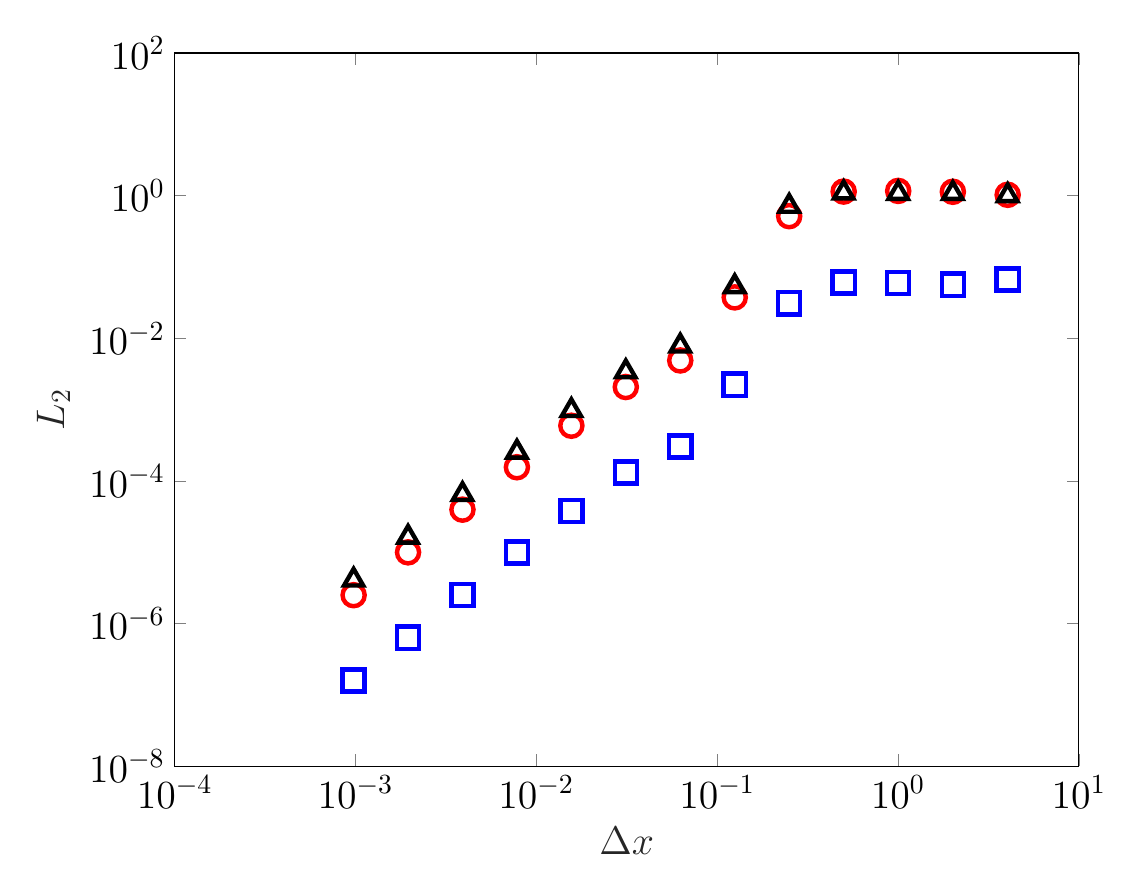
\begin{tikzpicture}
\tikzstyle{every node}=[font=\Large]

\begin{axis}[%
width=4.521in,
height=3.566in,
at={(0.758in,0.481in)},
every axis plot/.append style={ultra thick},
scale only axis,
xmode=log,
xmin=0.0001,
xmax=10,
xtick={0.0001,  0.001,   0.01,    0.1,      1,     10},
xminorticks=false,
xlabel style={font=\color{white!15!black}},
xlabel={\Large $\Delta x$},
ymode=log,
ymin=1e-08,
ymax=100,
ytick={ 1e-08,  1e-06, 0.0001,   0.01,      1,    100},
yminorticks=false,
ylabel style={font=\color{white!15!black}},
ylabel={\Large $L_2$},
axis background/.style={fill=white}
]
 \logLogSlopeTriangle{0.5}{0.2}{0.1}{2}{black};

\addplot [color=blue, draw=none, mark=square, mark size=4pt, mark options={solid, blue}, forget plot]
  table[row sep=crcr]{%
4.04040404040404	0.0667977316044187\\
2.01005025125628	0.0565251008982736\\
1.00250626566416	0.0600244047801842\\
0.500625782227785	0.060369043216863\\
0.250156347717323	0.031027562703989\\
0.125039074710847	0.00223720174663375\\
0.0625097671511174	0.000303213411708855\\
0.0312524415969998	0.00013195585438531\\
0.0156256103754053	3.78678120338089e-05\\
0.00781265259087092	9.90901359842452e-06\\
0.00390628814734519	2.52150220729934e-06\\
0.00195313453678973	6.35217079986901e-07\\
0.000976564884191612	1.59353271500116e-07\\
};
\addplot [color=red, draw=none, mark=o, mark size=4pt, mark options={solid, red}, forget plot]
  table[row sep=crcr]{%
4.04040404040404	1.02894168607817\\
2.01005025125628	1.13471870525711\\
1.00250626566416	1.16651134393852\\
0.500625782227785	1.14209935315627\\
0.250156347717323	0.516295949213657\\
0.125039074710847	0.0375055631709394\\
0.0625097671511174	0.0048956232734942\\
0.0312524415969998	0.00207713643544563\\
0.0156256103754053	0.000595469107815693\\
0.00781265259087092	0.00015580109802979\\
0.00390628814734519	3.96453330936357e-05\\
0.00195313453678973	9.98742874615667e-06\\
0.000976564884191612	2.5054904543415e-06\\
};
\addplot [color=black, draw=none, mark=triangle, mark size=4pt, mark options={solid, black}, forget plot]
  table[row sep=crcr]{%
4.04040404040404	1.00510027333734\\
2.01005025125628	1.07752750295002\\
1.00250626566416	1.07983904140976\\
0.500625782227785	1.09869881739817\\
0.250156347717323	0.712184449316794\\
0.125039074710847	0.05307095900171\\
0.0625097671511174	0.00781225049904385\\
0.0312524415969998	0.00340272133918679\\
0.0156256103754053	0.00097359240010264\\
0.00781265259087092	0.000254452413381455\\
0.00390628814734519	6.47146749585668e-05\\
0.00195313453678973	1.62988208772404e-05\\
0.000976564884191612	4.08829473005837e-06\\
};
%\addplot [color=mycolor1, forget plot]
%  table[row sep=crcr]{%
%4.04040404040404	16.3248648097133\\
%2.01005025125628	4.04030201257544\\
%1.00250626566416	1.0050188126959\\
%0.500625782227785	0.250626173831181\\
%0.250156347717323	0.0625781983032704\\
%0.125039074710847	0.0156347702045448\\
%0.0625097671511174	0.00390747098928691\\
%0.0312524415969998	0.000976715105773881\\
%0.0156256103754053	0.000244159699603973\\
%0.00781265259087092	6.1037540505642e-05\\
%0.00390628814734519	1.52590870900895e-05\\
%0.00195313453678973	3.81473451880083e-06\\
%0.000976564884191612	9.53678973036176e-07\\
%};
\end{axis}
\end{tikzpicture}%
\end{document}
	\caption{$L_2$ norm comparing numerical solution and analytic solution for travelling wave solution with $\beta_1 = \beta_2 = 0$. }
\end{figure}

\begin{figure}
	\centering
	\documentclass[]{standalone}
\usepackage{amsmath}
\usepackage{graphicx}
\usepackage[pdf]{pstricks}
\usepackage{pgfplots}
\pgfplotsset{compat=newest}
\usepgfplotslibrary{fillbetween}
%% the following commands are needed for some matlab2tikz features
\usetikzlibrary{plotmarks}
\usetikzlibrary{arrows.meta}
\usepgfplotslibrary{patchplots}
\usetikzlibrary{decorations.text}
\usetikzlibrary{shapes.multipart}

\newcommand{\logLogSlopeTriangle}[5]
{
	% #1. Relative offset in x direction.
	% #2. Width in x direction, so xA-xB.
	% #3. Relative offset in y direction.
	% #4. Slope d(y)/d(log10(x)).
	% #5. Plot options.
	
	\pgfplotsextra
	{
		\pgfkeysgetvalue{/pgfplots/xmin}{\xmin}
		\pgfkeysgetvalue{/pgfplots/xmax}{\xmax}
		\pgfkeysgetvalue{/pgfplots/ymin}{\ymin}
		\pgfkeysgetvalue{/pgfplots/ymax}{\ymax}
		
		% Calculate auxilliary quantities, in relative sense.
		\pgfmathsetmacro{\xArel}{#1}
		\pgfmathsetmacro{\yArel}{#3}
		\pgfmathsetmacro{\xBrel}{#1-#2}
		\pgfmathsetmacro{\yBrel}{\yArel}
		\pgfmathsetmacro{\xCrel}{\xArel}
		%\pgfmathsetmacro{\yCrel}{ln(\yC/exp(\ymin))/ln(exp(\ymax)/exp(\ymin))} % REPLACE THIS EXPRESSION WITH AN EXPRESSION INDEPENDENT OF \yC TO PREVENT THE 'DIMENSION TOO LARGE' ERROR.
		
		\pgfmathsetmacro{\lnxB}{\xmin*(1-(#1-#2))+\xmax*(#1-#2)} % in [xmin,xmax].
		\pgfmathsetmacro{\lnxA}{\xmin*(1-#1)+\xmax*#1} % in [xmin,xmax].
		\pgfmathsetmacro{\lnyA}{\ymin*(1-#3)+\ymax*#3} % in [ymin,ymax].
		\pgfmathsetmacro{\lnyC}{\lnyA+#4*(\lnxA-\lnxB)}
		\pgfmathsetmacro{\yCrel}{\lnyC-\ymin)/(\ymax-\ymin)} % THE IMPROVED EXPRESSION WITHOUT 'DIMENSION TOO LARGE' ERROR.
		
		% Define coordinates for \draw. MIND THE 'rel axis cs' as opposed to the 'axis cs'.
		\coordinate (A) at (rel axis cs:\xArel,\yArel);
		\coordinate (B) at (rel axis cs:\xBrel,\yBrel);
		\coordinate (C) at (rel axis cs:\xCrel,\yCrel);
		
		% Draw slope triangle.
		\draw[#5]   (A)-- node[pos=0.5,anchor=north] {1}
		(B)-- 
		(C)-- node[pos=0.5,anchor=west] {#4}
		cycle;
	}
}

\begin{document}
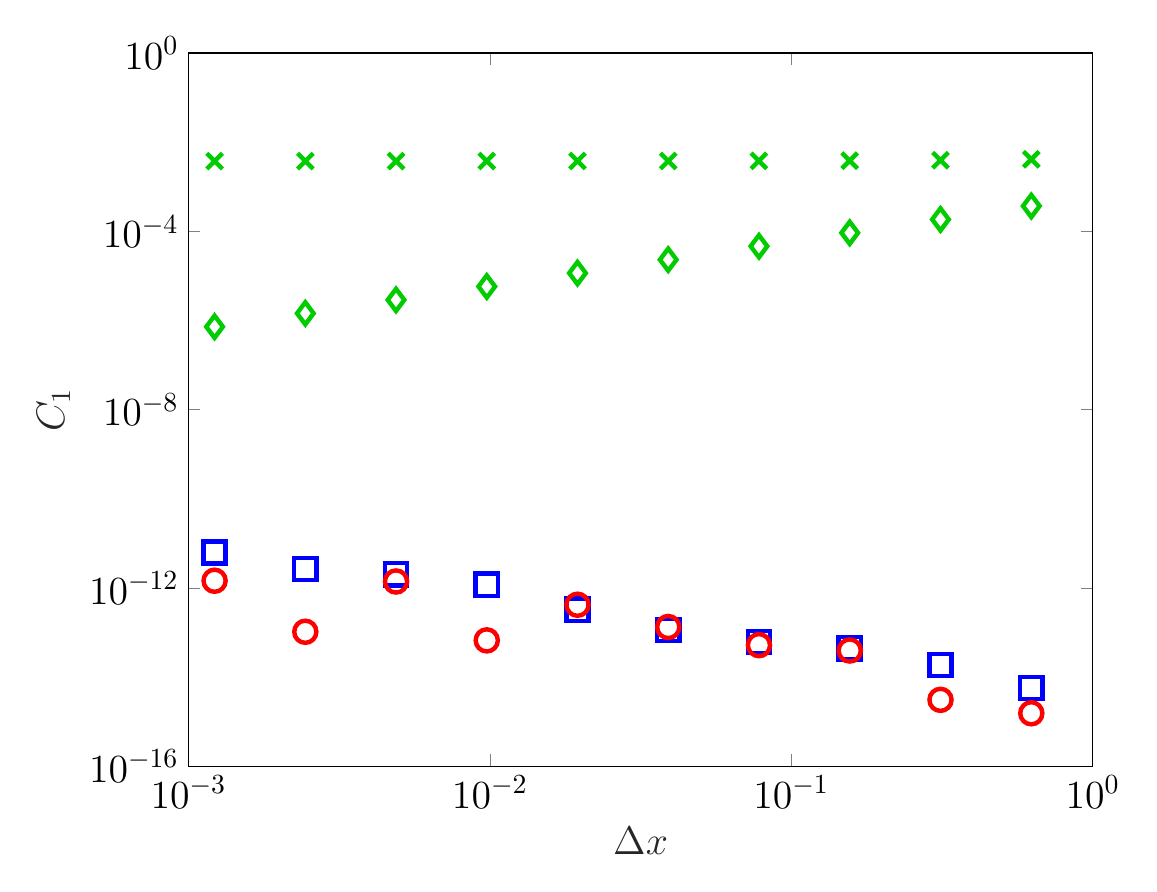
\begin{tikzpicture}
\tikzstyle{every node}=[font=\Large]
\begin{axis}[%
width=4.521in,
height=3.566in,
at={(0.758in,0.481in)},
every axis plot/.append style={ultra thick},
scale only axis,
xmode=log,
xmin=0.001,
xmax=1,
xtick={0.0001,  0.001,   0.01,    0.1,      1,     10},
xminorticks=false,
xlabel style={font=\color{white!15!black}},
xlabel={\Large $\Delta x$},
ymode=log,
ymin=1e-16,
ymax=1,
ytick={ 1e-16,  1e-12,  1e-08, 0.0001,      1},
yminorticks=true,
ylabel style={font=\color{white!15!black}},
ylabel={\Large $C_1$},
axis background/.style={fill=white},
legend style={at={(0.03,0.97)}, anchor=north west, legend cell align=left, align=left, draw=white!15!black}
]

\logLogSlopeTriangle{0.6}{0.5}{0.5}{1}{black};

\addplot [color=blue, draw=none, mark=square, mark size=4pt, mark options={solid, blue}]
  table[row sep=crcr]{%
5.05050505050505	3.56733880835235e-11\\
2.51256281407035	5.12803429349633e-15\\
1.2531328320802	5.29212229594127e-15\\
0.625782227784731	5.75293294483955e-15\\
0.312695434646654	1.84815007742139e-14\\
0.156298843388559	4.43997786684761e-14\\
0.0781372089388967	6.06235062150581e-14\\
0.0390655519962497	1.13374814721569e-13\\
0.0195320129692566	3.24676925344885e-13\\
0.00976581573858864	1.18307791711648e-12\\
0.00488286018418149	2.02072591105225e-12\\
0.00244141817098716	2.68072254395498e-12\\
0.00122070610523951	6.25791459992604e-12\\
};


\addplot [color=red, draw=none, mark=o, mark size=4pt, mark options={solid, red}]
  table[row sep=crcr]{%
5.05050505050505	2.29966242602921e-10\\
2.51256281407035	1.09744947528462e-15\\
1.2531328320802	2.42045514925841e-15\\
0.625782227784731	1.54476055254952e-15\\
0.312695434646654	3.08891006552572e-15\\
0.156298843388559	3.9506271121043e-14\\
0.0781372089388967	5.20946214173407e-14\\
0.0390655519962497	1.32882144892711e-13\\
0.0195320129692566	4.19611018204388e-13\\
0.00976581573858864	6.6662284399639e-14\\
0.00488286018418149	1.39572761789998e-12\\
0.00244141817098716	1.03968198317598e-13\\
0.00122070610523951	1.45092279397927e-12\\
};


%\addplot [color=black, draw=none, mark=triangle, mark size=4pt, mark options={solid, black}]
%  table[row sep=crcr]{%
%5.05050505050505	2.44257645831742e-06\\
%2.51256281407035	1.18170391007563e-06\\
%1.2531328320802	5.81157807324109e-07\\
%0.625782227784731	2.5388600240476e-07\\
%0.312695434646654	1.51556286613131e-07\\
%0.156298843388559	6.36004040868328e-08\\
%0.0781372089388967	3.42368613411178e-08\\
%0.0390655519962497	1.58421274216244e-08\\
%0.0195320129692566	8.62919552106989e-09\\
%0.00976581573858864	4.7145671141896e-09\\
%0.00488286018418149	2.26804766660682e-09\\
%0.00244141817098716	1.18110698751506e-09\\
%0.00122070610523951	5.64680035348884e-10\\
%};


\addplot [color=green, draw=none, mark=x, mark size=4pt, mark options={solid, green!80!black}]
  table[row sep=crcr]{%
5.05050505050505	0.00662111195170816\\
2.51256281407035	0.0052286494667814\\
1.2531328320802	0.00450358876669331\\
0.625782227784731	0.00413064267413027\\
0.312695434646654	0.00394934954073098\\
0.156298843388559	0.00385723425230475\\
0.0781372089388967	0.00381106943412185\\
0.0390655519962497	0.00378839592111398\\
0.0195320129692566	0.00377704290057945\\
0.00976581573858864	0.00377127202990541\\
0.00488286018418149	0.00376838958811927\\
0.00244141817098716	0.00376694735827935\\
0.00122070610523951	0.00376622673914215\\
};


\addplot [color=green, draw=none, only marks, mark=diamond, mark size=4pt, mark options={solid, green!80!black}, forget plot]
  table[row sep=crcr]{%
5.05050505050505	0.00286341532567191\\
2.51256281407035	0.00146591800971105\\
1.2531328320802	0.000738231083097194\\
0.625782227784731	0.00037015118303602\\
0.312695434646654	0.000185092664432067\\
0.156298843388559	9.26437920057067e-05\\
0.0781372089388967	4.63117777600743e-05\\
0.0390655519962497	2.31674191301811e-05\\
0.0195320129692566	1.1578907900003e-05\\
0.00976581573858864	5.78713356834035e-06\\
0.00488286018418149	2.89425127615534e-06\\
0.00244141817098716	1.44679737424634e-06\\
0.00122070610523951	7.23568057607806e-07\\
};

\end{axis}
\end{tikzpicture}%
\end{document}
	\caption{$C$ comparing total amount of conserved quantities in initial conditions and numerical solution for travelling wave solution with $\beta_1 = \beta_2 = 0$. }
\end{figure}


\subsubsection{Dam-break - SWWE ( $\beta_1= -\frac{2}{3}$ and $ \beta_2 =0$ ) }
\begin{align}
h(x,0) & = \left\lbrace \begin{array}{c c}
h_0 & x < 0\\
h_1 & x \ge 0
\end{array} \right.  \\
u(x,0) &= 0 \\
G(x,0) &= 0
\end{align}
$\Delta x \approx 0.02$
\begin{figure}
	\tikzset{every picture/.style={scale=0.6}}%
	\centering
	\begin{subfigure}{0.3\textwidth}
		\centering
		% This file was created by matlab2tikz.
%
%The latest updates can be retrieved from
%  http://www.mathworks.com/matlabcentral/fileexchange/22022-matlab2tikz-matlab2tikz
%where you can also make suggestions and rate matlab2tikz.
%
\begin{tikzpicture}

\begin{axis}[%
width=4.521in,
height=3.566in,
at={(0.758in,0.481in)},
scale only axis,
xmin=-100,
xmax=100,
xtick={-100,  -50,    0,   50,  100},
xlabel style={font=\color{white!15!black}},
xlabel={x (m)},
ymin=0.9,
ymax=2.1,
ytick={   1, 1.25,  1.5, 1.75,    2},
ylabel style={font=\color{white!15!black}},
ylabel={h (m)},
axis background/.style={fill=white}
]
\addplot [color=blue, forget plot]
  table[row sep=crcr]{%
-100.1200120012	2\\
-100.0200020002	2\\
-99.9199919991999	2\\
-99.8199819981998	2\\
-99.7199719971997	2\\
-99.6199619961996	2\\
-99.5199519951995	2\\
-99.4199419941994	2\\
-99.3199319931993	2\\
-99.2199219921992	2\\
-99.1199119911991	2\\
-99.019901990199	2\\
-98.9198919891989	2\\
-98.8198819881988	2\\
-98.7198719871987	2\\
-98.6198619861986	2\\
-98.5198519851985	2\\
-98.4198419841984	2\\
-98.3198319831983	2\\
-98.2198219821982	2\\
-98.1198119811981	2\\
-98.019801980198	2\\
-97.9197919791979	2\\
-97.8197819781978	2\\
-97.7197719771977	2\\
-97.6197619761976	2\\
-97.5197519751975	2\\
-97.4197419741974	2\\
-97.3197319731973	2\\
-97.2197219721972	2\\
-97.1197119711971	2\\
-97.019701970197	2\\
-96.9196919691969	2\\
-96.8196819681968	2\\
-96.7196719671967	2\\
-96.6196619661966	2\\
-96.5196519651965	2\\
-96.4196419641964	2\\
-96.3196319631963	2\\
-96.2196219621962	2\\
-96.1196119611961	2\\
-96.019601960196	2\\
-95.9195919591959	2\\
-95.8195819581958	2\\
-95.7195719571957	2\\
-95.6195619561956	2\\
-95.5195519551955	2\\
-95.4195419541954	2\\
-95.3195319531953	2\\
-95.2195219521952	2\\
-95.1195119511951	2\\
-95.019501950195	2\\
-94.9194919491949	2\\
-94.8194819481948	2\\
-94.7194719471947	2\\
-94.6194619461946	2\\
-94.5194519451945	2\\
-94.4194419441944	2\\
-94.3194319431943	2\\
-94.2194219421942	2\\
-94.1194119411941	2\\
-94.019401940194	2\\
-93.9193919391939	2\\
-93.8193819381938	2\\
-93.7193719371937	2\\
-93.6193619361936	2\\
-93.5193519351935	2\\
-93.4193419341934	2\\
-93.3193319331933	2\\
-93.2193219321932	2\\
-93.1193119311931	2\\
-93.019301930193	2\\
-92.9192919291929	2\\
-92.8192819281928	2\\
-92.7192719271927	2\\
-92.6192619261926	2\\
-92.5192519251925	2\\
-92.4192419241924	2\\
-92.3192319231923	2\\
-92.2192219221922	2\\
-92.1192119211921	2\\
-92.019201920192	2\\
-91.9191919191919	2\\
-91.8191819181918	2\\
-91.7191719171917	2\\
-91.6191619161916	2\\
-91.5191519151915	2\\
-91.4191419141914	2\\
-91.3191319131913	2\\
-91.2191219121912	2\\
-91.1191119111911	2\\
-91.019101910191	2\\
-90.9190919091909	2\\
-90.8190819081908	2\\
-90.7190719071907	2\\
-90.6190619061906	2\\
-90.5190519051905	2\\
-90.4190419041904	2\\
-90.3190319031903	2\\
-90.2190219021902	2\\
-90.1190119011901	2\\
-90.01900190019	2\\
-89.9189918991899	2\\
-89.8189818981898	2\\
-89.7189718971897	2\\
-89.6189618961896	2\\
-89.5189518951895	2\\
-89.4189418941894	2\\
-89.3189318931893	2\\
-89.2189218921892	2\\
-89.1189118911891	2\\
-89.018901890189	2\\
-88.9188918891889	2\\
-88.8188818881888	2\\
-88.7188718871887	2\\
-88.6188618861886	2\\
-88.5188518851885	2\\
-88.4188418841884	2\\
-88.3188318831883	2\\
-88.2188218821882	2\\
-88.1188118811881	2\\
-88.018801880188	2\\
-87.9187918791879	2\\
-87.8187818781878	2\\
-87.7187718771877	2\\
-87.6187618761876	2\\
-87.5187518751875	2\\
-87.4187418741874	2\\
-87.3187318731873	2\\
-87.2187218721872	2\\
-87.1187118711871	2\\
-87.018701870187	2\\
-86.9186918691869	2\\
-86.8186818681868	2\\
-86.7186718671867	2\\
-86.6186618661866	2\\
-86.5186518651865	2\\
-86.4186418641864	2\\
-86.3186318631863	2\\
-86.2186218621862	2\\
-86.1186118611861	2\\
-86.018601860186	2\\
-85.9185918591859	2\\
-85.8185818581858	2\\
-85.7185718571857	2\\
-85.6185618561856	2\\
-85.5185518551855	2\\
-85.4185418541854	2\\
-85.3185318531853	2\\
-85.2185218521852	2\\
-85.1185118511851	2\\
-85.018501850185	2\\
-84.9184918491849	2\\
-84.8184818481848	2\\
-84.7184718471847	2\\
-84.6184618461846	2\\
-84.5184518451845	2\\
-84.4184418441844	2\\
-84.3184318431843	2\\
-84.2184218421842	2\\
-84.1184118411841	2\\
-84.018401840184	2\\
-83.9183918391839	2\\
-83.8183818381838	2\\
-83.7183718371837	2\\
-83.6183618361836	2\\
-83.5183518351835	2\\
-83.4183418341834	2\\
-83.3183318331833	2\\
-83.2183218321832	2\\
-83.1183118311831	2\\
-83.018301830183	2\\
-82.9182918291829	2\\
-82.8182818281828	2\\
-82.7182718271827	2\\
-82.6182618261826	2\\
-82.5182518251825	2\\
-82.4182418241824	2\\
-82.3182318231823	2\\
-82.2182218221822	2\\
-82.1182118211821	2\\
-82.018201820182	2\\
-81.9181918191819	2\\
-81.8181818181818	2\\
-81.7181718171817	2\\
-81.6181618161816	2\\
-81.5181518151815	2\\
-81.4181418141814	2\\
-81.3181318131813	2\\
-81.2181218121812	2\\
-81.1181118111811	2\\
-81.018101810181	2\\
-80.9180918091809	2\\
-80.8180818081808	2\\
-80.7180718071807	2\\
-80.6180618061806	2\\
-80.5180518051805	2\\
-80.4180418041804	2\\
-80.3180318031803	2\\
-80.2180218021802	2\\
-80.1180118011801	2\\
-80.01800180018	2\\
-79.9179917991799	2\\
-79.8179817981798	2\\
-79.7179717971797	2\\
-79.6179617961796	2\\
-79.5179517951795	2\\
-79.4179417941794	2\\
-79.3179317931793	2\\
-79.2179217921792	2\\
-79.1179117911791	2\\
-79.017901790179	2\\
-78.9178917891789	2\\
-78.8178817881788	2\\
-78.7178717871787	2\\
-78.6178617861786	2\\
-78.5178517851785	2\\
-78.4178417841784	2\\
-78.3178317831783	2\\
-78.2178217821782	2\\
-78.1178117811781	2\\
-78.017801780178	2\\
-77.9177917791779	2\\
-77.8177817781778	2\\
-77.7177717771777	2\\
-77.6177617761776	2\\
-77.5177517751775	2\\
-77.4177417741774	2\\
-77.3177317731773	2\\
-77.2177217721772	2\\
-77.1177117711771	2\\
-77.017701770177	2\\
-76.9176917691769	2\\
-76.8176817681768	2\\
-76.7176717671767	2\\
-76.6176617661766	2\\
-76.5176517651765	2\\
-76.4176417641764	2\\
-76.3176317631763	2\\
-76.2176217621762	2\\
-76.1176117611761	2\\
-76.017601760176	2\\
-75.9175917591759	2\\
-75.8175817581758	2\\
-75.7175717571757	2\\
-75.6175617561756	2\\
-75.5175517551755	2\\
-75.4175417541754	2\\
-75.3175317531753	2\\
-75.2175217521752	2\\
-75.1175117511751	2\\
-75.017501750175	2\\
-74.9174917491749	2\\
-74.8174817481748	2\\
-74.7174717471747	2\\
-74.6174617461746	2\\
-74.5174517451745	2\\
-74.4174417441744	2\\
-74.3174317431743	2\\
-74.2174217421742	2\\
-74.1174117411741	2\\
-74.017401740174	2\\
-73.9173917391739	2\\
-73.8173817381738	2\\
-73.7173717371737	2\\
-73.6173617361736	2\\
-73.5173517351735	2\\
-73.4173417341734	2\\
-73.3173317331733	2\\
-73.2173217321732	2\\
-73.1173117311731	2\\
-73.017301730173	2\\
-72.9172917291729	2\\
-72.8172817281728	2\\
-72.7172717271727	2\\
-72.6172617261726	2\\
-72.5172517251725	2\\
-72.4172417241724	2\\
-72.3172317231723	2\\
-72.2172217221722	2\\
-72.1172117211721	2\\
-72.017201720172	2\\
-71.9171917191719	2\\
-71.8171817181718	2\\
-71.7171717171717	2\\
-71.6171617161716	2\\
-71.5171517151715	2\\
-71.4171417141714	2\\
-71.3171317131713	2\\
-71.2171217121712	2\\
-71.1171117111711	2\\
-71.017101710171	2\\
-70.9170917091709	2\\
-70.8170817081708	2\\
-70.7170717071707	2\\
-70.6170617061706	2\\
-70.5170517051705	2\\
-70.4170417041704	2\\
-70.3170317031703	2\\
-70.2170217021702	2\\
-70.1170117011701	2\\
-70.01700170017	2\\
-69.9169916991699	2\\
-69.8169816981698	2\\
-69.7169716971697	2\\
-69.6169616961696	2\\
-69.5169516951695	2\\
-69.4169416941694	2\\
-69.3169316931693	2\\
-69.2169216921692	2\\
-69.1169116911691	2\\
-69.016901690169	2\\
-68.9168916891689	2\\
-68.8168816881688	2\\
-68.7168716871687	2\\
-68.6168616861686	2\\
-68.5168516851685	2\\
-68.4168416841684	2\\
-68.3168316831683	2\\
-68.2168216821682	2\\
-68.1168116811681	2\\
-68.016801680168	2\\
-67.9167916791679	2\\
-67.8167816781678	2\\
-67.7167716771677	2\\
-67.6167616761676	2\\
-67.5167516751675	2\\
-67.4167416741674	2\\
-67.3167316731673	2\\
-67.2167216721672	2\\
-67.1167116711671	2\\
-67.016701670167	2\\
-66.9166916691669	2\\
-66.8166816681668	2\\
-66.7166716671667	2\\
-66.6166616661666	2\\
-66.5166516651665	2\\
-66.4166416641664	2\\
-66.3166316631663	2\\
-66.2166216621662	2\\
-66.1166116611661	2\\
-66.016601660166	2\\
-65.9165916591659	2\\
-65.8165816581658	2\\
-65.7165716571657	2\\
-65.6165616561656	2\\
-65.5165516551655	2\\
-65.4165416541654	2\\
-65.3165316531653	2\\
-65.2165216521652	2\\
-65.1165116511651	2\\
-65.016501650165	2\\
-64.9164916491649	2\\
-64.8164816481648	2\\
-64.7164716471647	2\\
-64.6164616461646	2\\
-64.5164516451645	2\\
-64.4164416441644	2\\
-64.3164316431643	2\\
-64.2164216421642	2\\
-64.1164116411641	2\\
-64.016401640164	2\\
-63.9163916391639	2\\
-63.8163816381638	2\\
-63.7163716371637	2\\
-63.6163616361636	2\\
-63.5163516351635	2\\
-63.4163416341634	2\\
-63.3163316331633	2\\
-63.2163216321632	2\\
-63.1163116311631	2\\
-63.016301630163	2\\
-62.9162916291629	2\\
-62.8162816281628	2\\
-62.7162716271627	2\\
-62.6162616261626	2\\
-62.5162516251625	2\\
-62.4162416241624	2\\
-62.3162316231623	2\\
-62.2162216221622	2\\
-62.1162116211621	2\\
-62.016201620162	2\\
-61.9161916191619	2\\
-61.8161816181618	2\\
-61.7161716171617	2\\
-61.6161616161616	2\\
-61.5161516151615	2\\
-61.4161416141614	2\\
-61.3161316131613	2\\
-61.2161216121612	2\\
-61.1161116111611	2\\
-61.016101610161	2\\
-60.9160916091609	2\\
-60.8160816081608	2\\
-60.7160716071607	2\\
-60.6160616061606	2\\
-60.5160516051605	2\\
-60.4160416041604	2\\
-60.3160316031603	2\\
-60.2160216021602	2\\
-60.1160116011601	2\\
-60.01600160016	2\\
-59.9159915991599	2\\
-59.8159815981598	2\\
-59.7159715971597	2\\
-59.6159615961596	2\\
-59.5159515951595	2\\
-59.4159415941594	2\\
-59.3159315931593	2\\
-59.2159215921592	2\\
-59.1159115911591	2\\
-59.015901590159	2\\
-58.9158915891589	2\\
-58.8158815881588	2\\
-58.7158715871587	2\\
-58.6158615861586	2\\
-58.5158515851585	2\\
-58.4158415841584	2\\
-58.3158315831583	2\\
-58.2158215821582	2\\
-58.1158115811581	2\\
-58.015801580158	2\\
-57.9157915791579	2\\
-57.8157815781578	2\\
-57.7157715771577	2\\
-57.6157615761576	2\\
-57.5157515751575	2\\
-57.4157415741574	2\\
-57.3157315731573	2\\
-57.2157215721572	2\\
-57.1157115711571	2\\
-57.015701570157	2\\
-56.9156915691569	2\\
-56.8156815681568	2\\
-56.7156715671567	2\\
-56.6156615661566	2\\
-56.5156515651565	2\\
-56.4156415641564	2\\
-56.3156315631563	2\\
-56.2156215621562	2\\
-56.1156115611561	2\\
-56.015601560156	2\\
-55.9155915591559	2\\
-55.8155815581558	2\\
-55.7155715571557	2\\
-55.6155615561556	2\\
-55.5155515551555	2\\
-55.4155415541554	2\\
-55.3155315531553	2\\
-55.2155215521552	2\\
-55.1155115511551	2\\
-55.015501550155	2\\
-54.9154915491549	2\\
-54.8154815481548	2\\
-54.7154715471547	2\\
-54.6154615461546	2\\
-54.5154515451545	2\\
-54.4154415441544	2\\
-54.3154315431543	2\\
-54.2154215421542	2\\
-54.1154115411541	2\\
-54.015401540154	2\\
-53.9153915391539	2\\
-53.8153815381538	2\\
-53.7153715371537	2\\
-53.6153615361536	2\\
-53.5153515351535	2\\
-53.4153415341534	2\\
-53.3153315331533	2\\
-53.2153215321532	2\\
-53.1153115311531	2\\
-53.015301530153	2\\
-52.9152915291529	2\\
-52.8152815281528	2\\
-52.7152715271527	2\\
-52.6152615261526	2\\
-52.5152515251525	2\\
-52.4152415241524	2\\
-52.3152315231523	2\\
-52.2152215221522	2\\
-52.1152115211521	2\\
-52.015201520152	2\\
-51.9151915191519	2\\
-51.8151815181518	2\\
-51.7151715171517	2\\
-51.6151615161516	2\\
-51.5151515151515	2\\
-51.4151415141514	2\\
-51.3151315131513	2\\
-51.2151215121512	2\\
-51.1151115111511	2\\
-51.015101510151	2\\
-50.9150915091509	2\\
-50.8150815081508	2\\
-50.7150715071507	2\\
-50.6150615061506	2\\
-50.5150515051505	2\\
-50.4150415041504	2\\
-50.3150315031503	2\\
-50.2150215021502	2\\
-50.1150115011501	2\\
-50.01500150015	2\\
-49.9149914991499	2\\
-49.8149814981498	2\\
-49.7149714971497	2\\
-49.6149614961496	2\\
-49.5149514951495	2\\
-49.4149414941494	2\\
-49.3149314931493	2\\
-49.2149214921492	2\\
-49.1149114911491	2\\
-49.014901490149	2\\
-48.9148914891489	2\\
-48.8148814881488	2\\
-48.7148714871487	2\\
-48.6148614861486	2\\
-48.5148514851485	2\\
-48.4148414841484	2\\
-48.3148314831483	2\\
-48.2148214821482	2\\
-48.1148114811481	2\\
-48.014801480148	2\\
-47.9147914791479	2\\
-47.8147814781478	2\\
-47.7147714771477	2\\
-47.6147614761476	2\\
-47.5147514751475	2\\
-47.4147414741474	2\\
-47.3147314731473	2\\
-47.2147214721472	2\\
-47.1147114711471	2\\
-47.014701470147	2\\
-46.9146914691469	2\\
-46.8146814681468	2\\
-46.7146714671467	2\\
-46.6146614661466	2\\
-46.5146514651465	2\\
-46.4146414641464	2\\
-46.3146314631463	2\\
-46.2146214621462	2\\
-46.1146114611461	2\\
-46.014601460146	2\\
-45.9145914591459	2\\
-45.8145814581458	2\\
-45.7145714571457	2\\
-45.6145614561456	2\\
-45.5145514551455	2\\
-45.4145414541454	2\\
-45.3145314531453	2\\
-45.2145214521452	2\\
-45.1145114511451	2\\
-45.014501450145	2\\
-44.9144914491449	2\\
-44.8144814481448	2\\
-44.7144714471447	2\\
-44.6144614461446	2\\
-44.5144514451445	2\\
-44.4144414441444	2\\
-44.3144314431443	2\\
-44.2144214421442	2\\
-44.1144114411441	2\\
-44.014401440144	2\\
-43.9143914391439	2\\
-43.8143814381438	2\\
-43.7143714371437	2\\
-43.6143614361436	2\\
-43.5143514351435	2\\
-43.4143414341434	2\\
-43.3143314331433	2\\
-43.2143214321432	2\\
-43.1143114311431	2\\
-43.014301430143	2\\
-42.9142914291429	2\\
-42.8142814281428	2\\
-42.7142714271427	2\\
-42.6142614261426	2\\
-42.5142514251425	2\\
-42.4142414241424	2\\
-42.3142314231423	2\\
-42.2142214221422	2\\
-42.1142114211421	2\\
-42.014201420142	2\\
-41.9141914191419	2\\
-41.8141814181418	2\\
-41.7141714171417	2\\
-41.6141614161416	2\\
-41.5141514151415	2\\
-41.4141414141414	2\\
-41.3141314131413	2\\
-41.2141214121412	2\\
-41.1141114111411	2\\
-41.014101410141	2\\
-40.9140914091409	2\\
-40.8140814081408	2\\
-40.7140714071407	2\\
-40.6140614061406	2\\
-40.5140514051405	2\\
-40.4140414041404	2\\
-40.3140314031403	2\\
-40.2140214021402	2\\
-40.1140114011401	2\\
-40.01400140014	2\\
-39.9139913991399	2\\
-39.8139813981398	2\\
-39.7139713971397	2\\
-39.6139613961396	2\\
-39.5139513951395	2\\
-39.4139413941394	2\\
-39.3139313931393	2\\
-39.2139213921392	2\\
-39.1139113911391	2\\
-39.013901390139	2\\
-38.9138913891389	2\\
-38.8138813881388	2\\
-38.7138713871387	2\\
-38.6138613861386	2\\
-38.5138513851385	2\\
-38.4138413841384	2\\
-38.3138313831383	2\\
-38.2138213821382	2\\
-38.1138113811381	2\\
-38.013801380138	2\\
-37.9137913791379	2\\
-37.8137813781378	2\\
-37.7137713771377	2\\
-37.6137613761376	2\\
-37.5137513751375	2\\
-37.4137413741374	2\\
-37.3137313731373	2\\
-37.2137213721372	2\\
-37.1137113711371	2\\
-37.013701370137	2\\
-36.9136913691369	2\\
-36.8136813681368	2\\
-36.7136713671367	2\\
-36.6136613661366	2\\
-36.5136513651365	2\\
-36.4136413641364	2\\
-36.3136313631363	2\\
-36.2136213621362	2\\
-36.1136113611361	2\\
-36.013601360136	2\\
-35.9135913591359	2\\
-35.8135813581358	2\\
-35.7135713571357	2\\
-35.6135613561356	2\\
-35.5135513551355	2\\
-35.4135413541354	2\\
-35.3135313531353	2\\
-35.2135213521352	2\\
-35.1135113511351	2\\
-35.013501350135	2\\
-34.9134913491349	2\\
-34.8134813481348	2\\
-34.7134713471347	2\\
-34.6134613461346	2\\
-34.5134513451345	2\\
-34.4134413441344	2\\
-34.3134313431343	2\\
-34.2134213421342	2\\
-34.1134113411341	2\\
-34.013401340134	2\\
-33.9133913391339	2\\
-33.8133813381338	2\\
-33.7133713371337	2\\
-33.6133613361336	2\\
-33.5133513351335	2\\
-33.4133413341334	2\\
-33.3133313331333	2\\
-33.2133213321332	2\\
-33.1133113311331	2\\
-33.013301330133	2\\
-32.9132913291329	2\\
-32.8132813281328	2\\
-32.7132713271327	2\\
-32.6132613261326	2\\
-32.5132513251325	2\\
-32.4132413241324	2\\
-32.3132313231323	2\\
-32.2132213221322	2\\
-32.1132113211321	2\\
-32.013201320132	2\\
-31.9131913191319	2\\
-31.8131813181318	2\\
-31.7131713171317	2\\
-31.6131613161316	2\\
-31.5131513151315	2\\
-31.4131413141314	2\\
-31.3131313131313	2\\
-31.2131213121312	2\\
-31.1131113111311	2\\
-31.013101310131	2\\
-30.9130913091309	2\\
-30.8130813081308	2\\
-30.7130713071307	2\\
-30.6130613061306	2\\
-30.5130513051305	2\\
-30.4130413041304	2\\
-30.3130313031303	2\\
-30.2130213021302	2\\
-30.1130113011301	2\\
-30.01300130013	2\\
-29.9129912991299	2\\
-29.8129812981298	2\\
-29.7129712971297	2\\
-29.6129612961296	2\\
-29.5129512951295	2\\
-29.4129412941294	2\\
-29.3129312931293	2\\
-29.2129212921292	2\\
-29.1129112911291	2\\
-29.012901290129	2\\
-28.9128912891289	2\\
-28.8128812881288	2\\
-28.7128712871287	2\\
-28.6128612861286	2\\
-28.5128512851285	2\\
-28.4128412841284	2\\
-28.3128312831283	2\\
-28.2128212821282	2\\
-28.1128112811281	2\\
-28.012801280128	2\\
-27.9127912791279	2\\
-27.8127812781278	2\\
-27.7127712771277	2\\
-27.6127612761276	2\\
-27.5127512751275	2\\
-27.4127412741274	2\\
-27.3127312731273	2\\
-27.2127212721272	2\\
-27.1127112711271	2\\
-27.012701270127	2\\
-26.9126912691269	2\\
-26.8126812681268	2\\
-26.7126712671267	2\\
-26.6126612661266	2\\
-26.5126512651265	2\\
-26.4126412641264	2\\
-26.3126312631263	2\\
-26.2126212621262	2\\
-26.1126112611261	2\\
-26.012601260126	2\\
-25.9125912591259	2\\
-25.8125812581258	2\\
-25.7125712571257	2\\
-25.6125612561256	2\\
-25.5125512551255	2\\
-25.4125412541254	2\\
-25.3125312531253	2\\
-25.2125212521252	2\\
-25.1125112511251	2\\
-25.012501250125	2\\
-24.9124912491249	2\\
-24.8124812481248	2\\
-24.7124712471247	2\\
-24.6124612461246	2\\
-24.5124512451245	2\\
-24.4124412441244	2\\
-24.3124312431243	2\\
-24.2124212421242	2\\
-24.1124112411241	2\\
-24.012401240124	2\\
-23.9123912391239	2\\
-23.8123812381238	2\\
-23.7123712371237	2\\
-23.6123612361236	2\\
-23.5123512351235	2\\
-23.4123412341234	2\\
-23.3123312331233	2\\
-23.2123212321232	2\\
-23.1123112311231	2\\
-23.012301230123	2\\
-22.9122912291229	2\\
-22.8122812281228	2\\
-22.7122712271227	2\\
-22.6122612261226	2\\
-22.5122512251225	2\\
-22.4122412241224	2\\
-22.3122312231223	2\\
-22.2122212221222	2\\
-22.1122112211221	2\\
-22.012201220122	2\\
-21.9121912191219	2\\
-21.8121812181218	2\\
-21.7121712171217	2\\
-21.6121612161216	2\\
-21.5121512151215	2\\
-21.4121412141214	2\\
-21.3121312131213	2\\
-21.2121212121212	2\\
-21.1121112111211	2\\
-21.012101210121	2\\
-20.9120912091209	2\\
-20.8120812081208	2\\
-20.7120712071207	2\\
-20.6120612061206	2\\
-20.5120512051205	2\\
-20.4120412041204	2\\
-20.3120312031203	2\\
-20.2120212021202	2\\
-20.1120112011201	2\\
-20.01200120012	2\\
-19.9119911991199	2\\
-19.8119811981198	2\\
-19.7119711971197	2\\
-19.6119611961196	2\\
-19.5119511951195	2\\
-19.4119411941194	2\\
-19.3119311931193	2\\
-19.2119211921192	2\\
-19.1119111911191	2\\
-19.011901190119	2\\
-18.9118911891189	2\\
-18.8118811881188	2\\
-18.7118711871187	2\\
-18.6118611861186	2\\
-18.5118511851185	2\\
-18.4118411841184	2\\
-18.3118311831183	2\\
-18.2118211821182	2\\
-18.1118111811181	2\\
-18.011801180118	2\\
-17.9117911791179	2\\
-17.8117811781178	2\\
-17.7117711771177	2\\
-17.6117611761176	2\\
-17.5117511751175	2\\
-17.4117411741174	2\\
-17.3117311731173	2\\
-17.2117211721172	2\\
-17.1117111711171	2\\
-17.011701170117	2\\
-16.9116911691169	2\\
-16.8116811681168	2\\
-16.7116711671167	2\\
-16.6116611661166	2\\
-16.5116511651165	2\\
-16.4116411641164	2\\
-16.3116311631163	2\\
-16.2116211621162	2\\
-16.1116111611161	2\\
-16.011601160116	2\\
-15.9115911591159	2\\
-15.8115811581158	2\\
-15.7115711571157	2\\
-15.6115611561156	2\\
-15.5115511551155	2\\
-15.4115411541154	2\\
-15.3115311531153	2\\
-15.2115211521152	2\\
-15.1115111511151	2\\
-15.011501150115	2\\
-14.9114911491149	2\\
-14.8114811481148	2\\
-14.7114711471147	2\\
-14.6114611461146	2\\
-14.5114511451145	2\\
-14.4114411441144	2\\
-14.3114311431143	2\\
-14.2114211421142	2\\
-14.1114111411141	2\\
-14.011401140114	2\\
-13.9113911391139	2\\
-13.8113811381138	2\\
-13.7113711371137	2\\
-13.6113611361136	2\\
-13.5113511351135	2\\
-13.4113411341134	2\\
-13.3113311331133	2\\
-13.2113211321132	2\\
-13.1113111311131	2\\
-13.011301130113	2\\
-12.9112911291129	2\\
-12.8112811281128	2\\
-12.7112711271127	2\\
-12.6112611261126	2\\
-12.5112511251125	2\\
-12.4112411241124	2\\
-12.3112311231123	2\\
-12.2112211221122	2\\
-12.1112111211121	2\\
-12.011201120112	2\\
-11.9111911191119	2\\
-11.8111811181118	2\\
-11.7111711171117	2\\
-11.6111611161116	2\\
-11.5111511151115	2\\
-11.4111411141114	2\\
-11.3111311131113	2\\
-11.2111211121112	2\\
-11.1111111111111	2\\
-11.011101110111	2\\
-10.9110911091109	2\\
-10.8110811081108	2\\
-10.7110711071107	2\\
-10.6110611061106	2\\
-10.5110511051105	2\\
-10.4110411041104	2\\
-10.3110311031103	2\\
-10.2110211021102	2\\
-10.1110111011101	2\\
-10.01100110011	2\\
-9.91099109910991	2\\
-9.81098109810981	2\\
-9.71097109710971	2\\
-9.61096109610961	2\\
-9.5109510951095	2\\
-9.4109410941094	2\\
-9.3109310931093	2\\
-9.2109210921092	2\\
-9.1109110911091	2\\
-9.010901090109	2\\
-8.9108910891089	2\\
-8.8108810881088	2\\
-8.7108710871087	2\\
-8.61086108610861	2\\
-8.51085108510851	2\\
-8.41084108410841	2\\
-8.31083108310831	2\\
-8.21082108210821	2\\
-8.11081108110811	2\\
-8.01080108010801	2\\
-7.91079107910791	2\\
-7.81078107810781	2\\
-7.71077107710771	2\\
-7.61076107610761	2\\
-7.51075107510751	2\\
-7.41074107410741	2\\
-7.31073107310731	2\\
-7.21072107210721	2\\
-7.1107110711071	2\\
-7.010701070107	2\\
-6.9106910691069	2\\
-6.8106810681068	2\\
-6.7106710671067	2\\
-6.6106610661066	2\\
-6.5106510651065	2\\
-6.4106410641064	2\\
-6.3106310631063	2\\
-6.2106210621062	2\\
-6.11061106110611	2\\
-6.01060106010601	2\\
-5.91059105910591	2\\
-5.81058105810581	2\\
-5.71057105710571	2\\
-5.61056105610561	2\\
-5.51055105510551	2\\
-5.41054105410541	2\\
-5.31053105310531	2\\
-5.21052105210521	2\\
-5.11051105110511	2\\
-5.01050105010501	2\\
-4.91049104910491	2\\
-4.8104810481048	2\\
-4.7104710471047	2\\
-4.6104610461046	2\\
-4.5104510451045	2\\
-4.4104410441044	2\\
-4.3104310431043	2\\
-4.2104210421042	2\\
-4.1104110411041	2\\
-4.010401040104	2\\
-3.9103910391039	2\\
-3.8103810381038	2\\
-3.71037103710371	2\\
-3.61036103610361	2\\
-3.51035103510351	2\\
-3.41034103410341	2\\
-3.31033103310331	2\\
-3.21032103210321	2\\
-3.11031103110311	2\\
-3.01030103010301	2\\
-2.91029102910291	2\\
-2.81028102810281	2\\
-2.71027102710271	2\\
-2.61026102610261	2\\
-2.51025102510251	2\\
-2.4102410241024	2\\
-2.3102310231023	2\\
-2.2102210221022	2\\
-2.1102110211021	2\\
-2.010201020102	2\\
-1.9101910191019	2\\
-1.8101810181018	2\\
-1.7101710171017	2\\
-1.6101610161016	2\\
-1.5101510151015	2\\
-1.4101410141014	2\\
-1.31013101310131	2\\
-1.21012101210121	2\\
-1.11011101110111	2\\
-1.01010101010101	2\\
-0.91009100910091	2\\
-0.810081008100809	2\\
-0.710071007100709	2\\
-0.610061006100608	2\\
-0.510051005100507	2\\
-0.410041004100407	2\\
-0.310031003100306	2\\
-0.210021002100206	2\\
-0.110011001100105	2\\
-0.0100010001000044	2\\
0.0900090009000962	1\\
0.190019001900197	1\\
0.290029002900297	1\\
0.390039003900398	1\\
0.490049004900499	1\\
0.590059005900599	1\\
0.6900690069007	1\\
0.7900790079008	1\\
0.890089008900901	1\\
0.990099009901002	1\\
1.09010901090109	1\\
1.19011901190119	1\\
1.29012901290129	1\\
1.39013901390139	1\\
1.49014901490149	1\\
1.59015901590159	1\\
1.69016901690169	1\\
1.79017901790179	1\\
1.89018901890189	1\\
1.99019901990199	1\\
2.09020902090209	1\\
2.19021902190219	1\\
2.2902290229023	1\\
2.3902390239024	1\\
2.4902490249025	1\\
2.5902590259026	1\\
2.6902690269027	1\\
2.7902790279028	1\\
2.8902890289029	1\\
2.990299029903	1\\
3.0903090309031	1\\
3.1903190319032	1\\
3.2903290329033	1\\
3.3903390339034	1\\
3.4903490349035	1\\
3.59035903590359	1\\
3.69036903690369	1\\
3.79037903790379	1\\
3.89038903890389	1\\
3.99039903990399	1\\
4.09040904090409	1\\
4.19041904190419	1\\
4.29042904290429	1\\
4.39043904390439	1\\
4.49044904490449	1\\
4.59045904590459	1\\
4.6904690469047	1\\
4.7904790479048	1\\
4.8904890489049	1\\
4.990499049905	1\\
5.0905090509051	1\\
5.1905190519052	1\\
5.2905290529053	1\\
5.3905390539054	1\\
5.4905490549055	1\\
5.5905590559056	1\\
5.6905690569057	1\\
5.7905790579058	1\\
5.8905890589059	1\\
5.99059905990599	1\\
6.09060906090609	1\\
6.19061906190619	1\\
6.29062906290629	1\\
6.39063906390639	1\\
6.49064906490649	1\\
6.59065906590659	1\\
6.69066906690669	1\\
6.79067906790679	1\\
6.89068906890689	1\\
6.990699069907	1\\
7.0907090709071	1\\
7.1907190719072	1\\
7.2907290729073	1\\
7.3907390739074	1\\
7.4907490749075	1\\
7.5907590759076	1\\
7.6907690769077	1\\
7.7907790779078	1\\
7.8907890789079	1\\
7.990799079908	1\\
8.0908090809081	1\\
8.1908190819082	1\\
8.2908290829083	1\\
8.39083908390839	1\\
8.49084908490849	1\\
8.59085908590859	1\\
8.69086908690869	1\\
8.79087908790879	1\\
8.89088908890889	1\\
8.99089908990899	1\\
9.09090909090909	1\\
9.19091909190919	1\\
9.29092909290929	1\\
9.3909390939094	1\\
9.4909490949095	1\\
9.5909590959096	1\\
9.6909690969097	1\\
9.7909790979098	1\\
9.8909890989099	1\\
9.99099909991	1\\
10.0910091009101	1\\
10.1910191019102	1\\
10.2910291029103	1\\
10.3910391039104	1\\
10.4910491049105	1\\
10.5910591059106	1\\
10.6910691069107	1\\
10.7910791079108	1\\
10.8910891089109	1\\
10.991099109911	1\\
11.0911091109111	1\\
11.1911191119112	1\\
11.2911291129113	1\\
11.3911391139114	1\\
11.4911491149115	1\\
11.5911591159116	1\\
11.6911691169117	1\\
11.7911791179118	1\\
11.8911891189119	1\\
11.991199119912	1\\
12.0912091209121	1\\
12.1912191219122	1\\
12.2912291229123	1\\
12.3912391239124	1\\
12.4912491249125	1\\
12.5912591259126	1\\
12.6912691269127	1\\
12.7912791279128	1\\
12.8912891289129	1\\
12.991299129913	1\\
13.0913091309131	1\\
13.1913191319132	1\\
13.2913291329133	1\\
13.3913391339134	1\\
13.4913491349135	1\\
13.5913591359136	1\\
13.6913691369137	1\\
13.7913791379138	1\\
13.8913891389139	1\\
13.991399139914	1\\
14.0914091409141	1\\
14.1914191419142	1\\
14.2914291429143	1\\
14.3914391439144	1\\
14.4914491449145	1\\
14.5914591459146	1\\
14.6914691469147	1\\
14.7914791479148	1\\
14.8914891489149	1\\
14.991499149915	1\\
15.0915091509151	1\\
15.1915191519152	1\\
15.2915291529153	1\\
15.3915391539154	1\\
15.4915491549155	1\\
15.5915591559156	1\\
15.6915691569157	1\\
15.7915791579158	1\\
15.8915891589159	1\\
15.991599159916	1\\
16.0916091609161	1\\
16.1916191619162	1\\
16.2916291629163	1\\
16.3916391639164	1\\
16.4916491649165	1\\
16.5916591659166	1\\
16.6916691669167	1\\
16.7916791679168	1\\
16.8916891689169	1\\
16.991699169917	1\\
17.0917091709171	1\\
17.1917191719172	1\\
17.2917291729173	1\\
17.3917391739174	1\\
17.4917491749175	1\\
17.5917591759176	1\\
17.6917691769177	1\\
17.7917791779178	1\\
17.8917891789179	1\\
17.991799179918	1\\
18.0918091809181	1\\
18.1918191819182	1\\
18.2918291829183	1\\
18.3918391839184	1\\
18.4918491849185	1\\
18.5918591859186	1\\
18.6918691869187	1\\
18.7918791879188	1\\
18.8918891889189	1\\
18.991899189919	1\\
19.0919091909191	1\\
19.1919191919192	1\\
19.2919291929193	1\\
19.3919391939194	1\\
19.4919491949195	1\\
19.5919591959196	1\\
19.6919691969197	1\\
19.7919791979198	1\\
19.8919891989199	1\\
19.99199919992	1\\
20.0920092009201	1\\
20.1920192019202	1\\
20.2920292029203	1\\
20.3920392039204	1\\
20.4920492049205	1\\
20.5920592059206	1\\
20.6920692069207	1\\
20.7920792079208	1\\
20.8920892089209	1\\
20.992099209921	1\\
21.0921092109211	1\\
21.1921192119212	1\\
21.2921292129213	1\\
21.3921392139214	1\\
21.4921492149215	1\\
21.5921592159216	1\\
21.6921692169217	1\\
21.7921792179218	1\\
21.8921892189219	1\\
21.992199219922	1\\
22.0922092209221	1\\
22.1922192219222	1\\
22.2922292229223	1\\
22.3922392239224	1\\
22.4922492249225	1\\
22.5922592259226	1\\
22.6922692269227	1\\
22.7922792279228	1\\
22.8922892289229	1\\
22.992299229923	1\\
23.0923092309231	1\\
23.1923192319232	1\\
23.2923292329233	1\\
23.3923392339234	1\\
23.4923492349235	1\\
23.5923592359236	1\\
23.6923692369237	1\\
23.7923792379238	1\\
23.8923892389239	1\\
23.992399239924	1\\
24.0924092409241	1\\
24.1924192419242	1\\
24.2924292429243	1\\
24.3924392439244	1\\
24.4924492449245	1\\
24.5924592459246	1\\
24.6924692469247	1\\
24.7924792479248	1\\
24.8924892489249	1\\
24.992499249925	1\\
25.0925092509251	1\\
25.1925192519252	1\\
25.2925292529253	1\\
25.3925392539254	1\\
25.4925492549255	1\\
25.5925592559256	1\\
25.6925692569257	1\\
25.7925792579258	1\\
25.8925892589259	1\\
25.992599259926	1\\
26.0926092609261	1\\
26.1926192619262	1\\
26.2926292629263	1\\
26.3926392639264	1\\
26.4926492649265	1\\
26.5926592659266	1\\
26.6926692669267	1\\
26.7926792679268	1\\
26.8926892689269	1\\
26.992699269927	1\\
27.0927092709271	1\\
27.1927192719272	1\\
27.2927292729273	1\\
27.3927392739274	1\\
27.4927492749275	1\\
27.5927592759276	1\\
27.6927692769277	1\\
27.7927792779278	1\\
27.8927892789279	1\\
27.992799279928	1\\
28.0928092809281	1\\
28.1928192819282	1\\
28.2928292829283	1\\
28.3928392839284	1\\
28.4928492849285	1\\
28.5928592859286	1\\
28.6928692869287	1\\
28.7928792879288	1\\
28.8928892889289	1\\
28.992899289929	1\\
29.0929092909291	1\\
29.1929192919292	1\\
29.2929292929293	1\\
29.3929392939294	1\\
29.4929492949295	1\\
29.5929592959296	1\\
29.6929692969297	1\\
29.7929792979298	1\\
29.8929892989299	1\\
29.99299929993	1\\
30.0930093009301	1\\
30.1930193019302	1\\
30.2930293029303	1\\
30.3930393039304	1\\
30.4930493049305	1\\
30.5930593059306	1\\
30.6930693069307	1\\
30.7930793079308	1\\
30.8930893089309	1\\
30.993099309931	1\\
31.0931093109311	1\\
31.1931193119312	1\\
31.2931293129313	1\\
31.3931393139314	1\\
31.4931493149315	1\\
31.5931593159316	1\\
31.6931693169317	1\\
31.7931793179318	1\\
31.8931893189319	1\\
31.993199319932	1\\
32.0932093209321	1\\
32.1932193219322	1\\
32.2932293229323	1\\
32.3932393239324	1\\
32.4932493249325	1\\
32.5932593259326	1\\
32.6932693269327	1\\
32.7932793279328	1\\
32.8932893289329	1\\
32.993299329933	1\\
33.0933093309331	1\\
33.1933193319332	1\\
33.2933293329333	1\\
33.3933393339334	1\\
33.4933493349335	1\\
33.5933593359336	1\\
33.6933693369337	1\\
33.7933793379338	1\\
33.8933893389339	1\\
33.993399339934	1\\
34.0934093409341	1\\
34.1934193419342	1\\
34.2934293429343	1\\
34.3934393439344	1\\
34.4934493449345	1\\
34.5934593459346	1\\
34.6934693469347	1\\
34.7934793479348	1\\
34.8934893489349	1\\
34.993499349935	1\\
35.0935093509351	1\\
35.1935193519352	1\\
35.2935293529353	1\\
35.3935393539354	1\\
35.4935493549355	1\\
35.5935593559356	1\\
35.6935693569357	1\\
35.7935793579358	1\\
35.8935893589359	1\\
35.993599359936	1\\
36.0936093609361	1\\
36.1936193619362	1\\
36.2936293629363	1\\
36.3936393639364	1\\
36.4936493649365	1\\
36.5936593659366	1\\
36.6936693669367	1\\
36.7936793679368	1\\
36.8936893689369	1\\
36.993699369937	1\\
37.0937093709371	1\\
37.1937193719372	1\\
37.2937293729373	1\\
37.3937393739374	1\\
37.4937493749375	1\\
37.5937593759376	1\\
37.6937693769377	1\\
37.7937793779378	1\\
37.8937893789379	1\\
37.993799379938	1\\
38.0938093809381	1\\
38.1938193819382	1\\
38.2938293829383	1\\
38.3938393839384	1\\
38.4938493849385	1\\
38.5938593859386	1\\
38.6938693869387	1\\
38.7938793879388	1\\
38.8938893889389	1\\
38.993899389939	1\\
39.0939093909391	1\\
39.1939193919392	1\\
39.2939293929393	1\\
39.3939393939394	1\\
39.4939493949395	1\\
39.5939593959396	1\\
39.6939693969397	1\\
39.7939793979398	1\\
39.8939893989399	1\\
39.99399939994	1\\
40.0940094009401	1\\
40.1940194019402	1\\
40.2940294029403	1\\
40.3940394039404	1\\
40.4940494049405	1\\
40.5940594059406	1\\
40.6940694069407	1\\
40.7940794079408	1\\
40.8940894089409	1\\
40.994099409941	1\\
41.0941094109411	1\\
41.1941194119412	1\\
41.2941294129413	1\\
41.3941394139414	1\\
41.4941494149415	1\\
41.5941594159416	1\\
41.6941694169417	1\\
41.7941794179418	1\\
41.8941894189419	1\\
41.994199419942	1\\
42.0942094209421	1\\
42.1942194219422	1\\
42.2942294229423	1\\
42.3942394239424	1\\
42.4942494249425	1\\
42.5942594259426	1\\
42.6942694269427	1\\
42.7942794279428	1\\
42.8942894289429	1\\
42.994299429943	1\\
43.0943094309431	1\\
43.1943194319432	1\\
43.2943294329433	1\\
43.3943394339434	1\\
43.4943494349435	1\\
43.5943594359436	1\\
43.6943694369437	1\\
43.7943794379438	1\\
43.8943894389439	1\\
43.994399439944	1\\
44.0944094409441	1\\
44.1944194419442	1\\
44.2944294429443	1\\
44.3944394439444	1\\
44.4944494449445	1\\
44.5944594459446	1\\
44.6944694469447	1\\
44.7944794479448	1\\
44.8944894489449	1\\
44.994499449945	1\\
45.0945094509451	1\\
45.1945194519452	1\\
45.2945294529453	1\\
45.3945394539454	1\\
45.4945494549455	1\\
45.5945594559456	1\\
45.6945694569457	1\\
45.7945794579458	1\\
45.8945894589459	1\\
45.994599459946	1\\
46.0946094609461	1\\
46.1946194619462	1\\
46.2946294629463	1\\
46.3946394639464	1\\
46.4946494649465	1\\
46.5946594659466	1\\
46.6946694669467	1\\
46.7946794679468	1\\
46.8946894689469	1\\
46.994699469947	1\\
47.0947094709471	1\\
47.1947194719472	1\\
47.2947294729473	1\\
47.3947394739474	1\\
47.4947494749475	1\\
47.5947594759476	1\\
47.6947694769477	1\\
47.7947794779478	1\\
47.8947894789479	1\\
47.994799479948	1\\
48.0948094809481	1\\
48.1948194819482	1\\
48.2948294829483	1\\
48.3948394839484	1\\
48.4948494849485	1\\
48.5948594859486	1\\
48.6948694869487	1\\
48.7948794879488	1\\
48.8948894889489	1\\
48.994899489949	1\\
49.0949094909491	1\\
49.1949194919492	1\\
49.2949294929493	1\\
49.3949394939494	1\\
49.4949494949495	1\\
49.5949594959496	1\\
49.6949694969497	1\\
49.7949794979498	1\\
49.8949894989499	1\\
49.99499949995	1\\
50.0950095009501	1\\
50.1950195019502	1\\
50.2950295029503	1\\
50.3950395039504	1\\
50.4950495049505	1\\
50.5950595059506	1\\
50.6950695069507	1\\
50.7950795079508	1\\
50.8950895089509	1\\
50.995099509951	1\\
51.0951095109511	1\\
51.1951195119512	1\\
51.2951295129513	1\\
51.3951395139514	1\\
51.4951495149515	1\\
51.5951595159516	1\\
51.6951695169517	1\\
51.7951795179518	1\\
51.8951895189519	1\\
51.995199519952	1\\
52.0952095209521	1\\
52.1952195219522	1\\
52.2952295229523	1\\
52.3952395239524	1\\
52.4952495249525	1\\
52.5952595259526	1\\
52.6952695269527	1\\
52.7952795279528	1\\
52.8952895289529	1\\
52.995299529953	1\\
53.0953095309531	1\\
53.1953195319532	1\\
53.2953295329533	1\\
53.3953395339534	1\\
53.4953495349535	1\\
53.5953595359536	1\\
53.6953695369537	1\\
53.7953795379538	1\\
53.8953895389539	1\\
53.995399539954	1\\
54.0954095409541	1\\
54.1954195419542	1\\
54.2954295429543	1\\
54.3954395439544	1\\
54.4954495449545	1\\
54.5954595459546	1\\
54.6954695469547	1\\
54.7954795479548	1\\
54.8954895489549	1\\
54.995499549955	1\\
55.0955095509551	1\\
55.1955195519552	1\\
55.2955295529553	1\\
55.3955395539554	1\\
55.4955495549555	1\\
55.5955595559556	1\\
55.6955695569557	1\\
55.7955795579558	1\\
55.8955895589559	1\\
55.995599559956	1\\
56.0956095609561	1\\
56.1956195619562	1\\
56.2956295629563	1\\
56.3956395639564	1\\
56.4956495649565	1\\
56.5956595659566	1\\
56.6956695669567	1\\
56.7956795679568	1\\
56.8956895689569	1\\
56.995699569957	1\\
57.0957095709571	1\\
57.1957195719572	1\\
57.2957295729573	1\\
57.3957395739574	1\\
57.4957495749575	1\\
57.5957595759576	1\\
57.6957695769577	1\\
57.7957795779578	1\\
57.8957895789579	1\\
57.995799579958	1\\
58.0958095809581	1\\
58.1958195819582	1\\
58.2958295829583	1\\
58.3958395839584	1\\
58.4958495849585	1\\
58.5958595859586	1\\
58.6958695869587	1\\
58.7958795879588	1\\
58.8958895889589	1\\
58.995899589959	1\\
59.0959095909591	1\\
59.1959195919592	1\\
59.2959295929593	1\\
59.3959395939594	1\\
59.4959495949595	1\\
59.5959595959596	1\\
59.6959695969597	1\\
59.7959795979598	1\\
59.8959895989599	1\\
59.99599959996	1\\
60.0960096009601	1\\
60.1960196019602	1\\
60.2960296029603	1\\
60.3960396039604	1\\
60.4960496049605	1\\
60.5960596059606	1\\
60.6960696069607	1\\
60.7960796079608	1\\
60.8960896089609	1\\
60.996099609961	1\\
61.0961096109611	1\\
61.1961196119612	1\\
61.2961296129613	1\\
61.3961396139614	1\\
61.4961496149615	1\\
61.5961596159616	1\\
61.6961696169617	1\\
61.7961796179618	1\\
61.8961896189619	1\\
61.996199619962	1\\
62.0962096209621	1\\
62.1962196219622	1\\
62.2962296229623	1\\
62.3962396239624	1\\
62.4962496249625	1\\
62.5962596259626	1\\
62.6962696269627	1\\
62.7962796279628	1\\
62.8962896289629	1\\
62.996299629963	1\\
63.0963096309631	1\\
63.1963196319632	1\\
63.2963296329633	1\\
63.3963396339634	1\\
63.4963496349635	1\\
63.5963596359636	1\\
63.6963696369637	1\\
63.7963796379638	1\\
63.8963896389639	1\\
63.996399639964	1\\
64.0964096409641	1\\
64.1964196419642	1\\
64.2964296429643	1\\
64.3964396439644	1\\
64.4964496449645	1\\
64.5964596459646	1\\
64.6964696469647	1\\
64.7964796479648	1\\
64.8964896489649	1\\
64.996499649965	1\\
65.0965096509651	1\\
65.1965196519652	1\\
65.2965296529653	1\\
65.3965396539654	1\\
65.4965496549655	1\\
65.5965596559656	1\\
65.6965696569657	1\\
65.7965796579658	1\\
65.8965896589659	1\\
65.996599659966	1\\
66.0966096609661	1\\
66.1966196619662	1\\
66.2966296629663	1\\
66.3966396639664	1\\
66.4966496649665	1\\
66.5966596659666	1\\
66.6966696669667	1\\
66.7966796679668	1\\
66.8966896689669	1\\
66.996699669967	1\\
67.0967096709671	1\\
67.1967196719672	1\\
67.2967296729673	1\\
67.3967396739674	1\\
67.4967496749675	1\\
67.5967596759676	1\\
67.6967696769677	1\\
67.7967796779678	1\\
67.8967896789679	1\\
67.996799679968	1\\
68.0968096809681	1\\
68.1968196819682	1\\
68.2968296829683	1\\
68.3968396839684	1\\
68.4968496849685	1\\
68.5968596859686	1\\
68.6968696869687	1\\
68.7968796879688	1\\
68.8968896889689	1\\
68.996899689969	1\\
69.0969096909691	1\\
69.1969196919692	1\\
69.2969296929693	1\\
69.3969396939694	1\\
69.4969496949695	1\\
69.5969596959696	1\\
69.6969696969697	1\\
69.7969796979698	1\\
69.8969896989699	1\\
69.99699969997	1\\
70.0970097009701	1\\
70.1970197019702	1\\
70.2970297029703	1\\
70.3970397039704	1\\
70.4970497049705	1\\
70.5970597059706	1\\
70.6970697069707	1\\
70.7970797079708	1\\
70.8970897089709	1\\
70.997099709971	1\\
71.0971097109711	1\\
71.1971197119712	1\\
71.2971297129713	1\\
71.3971397139714	1\\
71.4971497149715	1\\
71.5971597159716	1\\
71.6971697169717	1\\
71.7971797179718	1\\
71.8971897189719	1\\
71.997199719972	1\\
72.0972097209721	1\\
72.1972197219722	1\\
72.2972297229723	1\\
72.3972397239724	1\\
72.4972497249725	1\\
72.5972597259726	1\\
72.6972697269727	1\\
72.7972797279728	1\\
72.8972897289729	1\\
72.997299729973	1\\
73.0973097309731	1\\
73.1973197319732	1\\
73.2973297329733	1\\
73.3973397339734	1\\
73.4973497349735	1\\
73.5973597359736	1\\
73.6973697369737	1\\
73.7973797379738	1\\
73.8973897389739	1\\
73.997399739974	1\\
74.0974097409741	1\\
74.1974197419742	1\\
74.2974297429743	1\\
74.3974397439744	1\\
74.4974497449745	1\\
74.5974597459746	1\\
74.6974697469747	1\\
74.7974797479748	1\\
74.8974897489749	1\\
74.997499749975	1\\
75.0975097509751	1\\
75.1975197519752	1\\
75.2975297529753	1\\
75.3975397539754	1\\
75.4975497549755	1\\
75.5975597559756	1\\
75.6975697569757	1\\
75.7975797579758	1\\
75.8975897589759	1\\
75.997599759976	1\\
76.0976097609761	1\\
76.1976197619762	1\\
76.2976297629763	1\\
76.3976397639764	1\\
76.4976497649765	1\\
76.5976597659766	1\\
76.6976697669767	1\\
76.7976797679768	1\\
76.8976897689769	1\\
76.997699769977	1\\
77.0977097709771	1\\
77.1977197719772	1\\
77.2977297729773	1\\
77.3977397739774	1\\
77.4977497749775	1\\
77.5977597759776	1\\
77.6977697769777	1\\
77.7977797779778	1\\
77.8977897789779	1\\
77.997799779978	1\\
78.0978097809781	1\\
78.1978197819782	1\\
78.2978297829783	1\\
78.3978397839784	1\\
78.4978497849785	1\\
78.5978597859786	1\\
78.6978697869787	1\\
78.7978797879788	1\\
78.8978897889789	1\\
78.997899789979	1\\
79.0979097909791	1\\
79.1979197919792	1\\
79.2979297929793	1\\
79.3979397939794	1\\
79.4979497949795	1\\
79.5979597959796	1\\
79.6979697969797	1\\
79.7979797979798	1\\
79.8979897989799	1\\
79.99799979998	1\\
80.0980098009801	1\\
80.1980198019802	1\\
80.2980298029803	1\\
80.3980398039804	1\\
80.4980498049805	1\\
80.5980598059806	1\\
80.6980698069807	1\\
80.7980798079808	1\\
80.8980898089809	1\\
80.998099809981	1\\
81.0981098109811	1\\
81.1981198119812	1\\
81.2981298129813	1\\
81.3981398139814	1\\
81.4981498149815	1\\
81.5981598159816	1\\
81.6981698169817	1\\
81.7981798179818	1\\
81.8981898189819	1\\
81.998199819982	1\\
82.0982098209821	1\\
82.1982198219822	1\\
82.2982298229823	1\\
82.3982398239824	1\\
82.4982498249825	1\\
82.5982598259826	1\\
82.6982698269827	1\\
82.7982798279828	1\\
82.8982898289829	1\\
82.998299829983	1\\
83.0983098309831	1\\
83.1983198319832	1\\
83.2983298329833	1\\
83.3983398339834	1\\
83.4983498349835	1\\
83.5983598359836	1\\
83.6983698369837	1\\
83.7983798379838	1\\
83.8983898389839	1\\
83.998399839984	1\\
84.0984098409841	1\\
84.1984198419842	1\\
84.2984298429843	1\\
84.3984398439844	1\\
84.4984498449845	1\\
84.5984598459846	1\\
84.6984698469847	1\\
84.7984798479848	1\\
84.8984898489849	1\\
84.998499849985	1\\
85.0985098509851	1\\
85.1985198519852	1\\
85.2985298529853	1\\
85.3985398539854	1\\
85.4985498549855	1\\
85.5985598559856	1\\
85.6985698569857	1\\
85.7985798579858	1\\
85.8985898589859	1\\
85.998599859986	1\\
86.0986098609861	1\\
86.1986198619862	1\\
86.2986298629863	1\\
86.3986398639864	1\\
86.4986498649865	1\\
86.5986598659866	1\\
86.6986698669867	1\\
86.7986798679868	1\\
86.8986898689869	1\\
86.998699869987	1\\
87.0987098709871	1\\
87.1987198719872	1\\
87.2987298729873	1\\
87.3987398739874	1\\
87.4987498749875	1\\
87.5987598759876	1\\
87.6987698769877	1\\
87.7987798779878	1\\
87.8987898789879	1\\
87.998799879988	1\\
88.0988098809881	1\\
88.1988198819882	1\\
88.2988298829883	1\\
88.3988398839884	1\\
88.4988498849885	1\\
88.5988598859886	1\\
88.6988698869887	1\\
88.7988798879888	1\\
88.8988898889889	1\\
88.998899889989	1\\
89.0989098909891	1\\
89.1989198919892	1\\
89.2989298929893	1\\
89.3989398939894	1\\
89.4989498949895	1\\
89.5989598959896	1\\
89.6989698969897	1\\
89.7989798979898	1\\
89.8989898989899	1\\
89.99899989999	1\\
90.0990099009901	1\\
90.1990199019902	1\\
90.2990299029903	1\\
90.3990399039904	1\\
90.4990499049905	1\\
90.5990599059906	1\\
90.6990699069907	1\\
90.7990799079908	1\\
90.8990899089909	1\\
90.999099909991	1\\
91.0991099109911	1\\
91.1991199119912	1\\
91.2991299129913	1\\
91.3991399139914	1\\
91.4991499149915	1\\
91.5991599159916	1\\
91.6991699169917	1\\
91.7991799179918	1\\
91.8991899189919	1\\
91.999199919992	1\\
92.0992099209921	1\\
92.1992199219922	1\\
92.2992299229923	1\\
92.3992399239924	1\\
92.4992499249925	1\\
92.5992599259926	1\\
92.6992699269927	1\\
92.7992799279928	1\\
92.8992899289929	1\\
92.999299929993	1\\
93.0993099309931	1\\
93.1993199319932	1\\
93.2993299329933	1\\
93.3993399339934	1\\
93.4993499349935	1\\
93.5993599359936	1\\
93.6993699369937	1\\
93.7993799379938	1\\
93.8993899389939	1\\
93.999399939994	1\\
94.0994099409941	1\\
94.1994199419942	1\\
94.2994299429943	1\\
94.3994399439944	1\\
94.4994499449945	1\\
94.5994599459946	1\\
94.6994699469947	1\\
94.7994799479948	1\\
94.8994899489949	1\\
94.999499949995	1\\
95.0995099509951	1\\
95.1995199519952	1\\
95.2995299529953	1\\
95.3995399539954	1\\
95.4995499549955	1\\
95.5995599559956	1\\
95.6995699569957	1\\
95.7995799579958	1\\
95.8995899589959	1\\
95.999599959996	1\\
96.0996099609961	1\\
96.1996199619962	1\\
96.2996299629963	1\\
96.3996399639964	1\\
96.4996499649965	1\\
96.5996599659966	1\\
96.6996699669967	1\\
96.7996799679968	1\\
96.8996899689969	1\\
96.999699969997	1\\
97.0997099709971	1\\
97.1997199719972	1\\
97.2997299729973	1\\
97.3997399739974	1\\
97.4997499749975	1\\
97.5997599759976	1\\
97.6997699769977	1\\
97.7997799779978	1\\
97.8997899789979	1\\
97.999799979998	1\\
98.0998099809981	1\\
98.1998199819982	1\\
98.2998299829983	1\\
98.3998399839984	1\\
98.4998499849985	1\\
98.5998599859986	1\\
98.6998699869987	1\\
98.7998799879988	1\\
98.8998899889989	1\\
98.999899989999	1\\
99.0999099909991	1\\
99.1999199919992	1\\
99.2999299929993	1\\
99.3999399939994	1\\
99.4999499949995	1\\
99.5999599959996	1\\
99.6999699969997	1\\
99.7999799979998	1\\
99.8999899989999	1\\
100	1\\
100.100010001	1\\
};
\end{axis}
\end{tikzpicture}%
		\caption{$h$}
	\end{subfigure}
	\begin{subfigure}{0.3\textwidth}
		\centering
		% This file was created by matlab2tikz.
%
%The latest updates can be retrieved from
%  http://www.mathworks.com/matlabcentral/fileexchange/22022-matlab2tikz-matlab2tikz
%where you can also make suggestions and rate matlab2tikz.
%
\begin{tikzpicture}

\begin{axis}[%
width=4.521in,
height=3.566in,
at={(0.758in,0.481in)},
scale only axis,
xmin=-100,
xmax=100,
xtick={-100,  -50,    0,   50,  100},
xlabel style={font=\color{white!15!black}},
xlabel={x (m)},
ymin=-0.1,
ymax=0.1,
ytick={-0.1,    0,  0.1},
ylabel style={font=\color{white!15!black}},
ylabel={u (m/s)},
axis background/.style={fill=white}
]
\addplot [color=red, forget plot]
  table[row sep=crcr]{%
-100.1200120012	0\\
-100.0200020002	0\\
-99.9199919991999	0\\
-99.8199819981998	0\\
-99.7199719971997	0\\
-99.6199619961996	0\\
-99.5199519951995	0\\
-99.4199419941994	0\\
-99.3199319931993	0\\
-99.2199219921992	0\\
-99.1199119911991	0\\
-99.019901990199	0\\
-98.9198919891989	0\\
-98.8198819881988	0\\
-98.7198719871987	0\\
-98.6198619861986	0\\
-98.5198519851985	0\\
-98.4198419841984	0\\
-98.3198319831983	0\\
-98.2198219821982	0\\
-98.1198119811981	0\\
-98.019801980198	0\\
-97.9197919791979	0\\
-97.8197819781978	0\\
-97.7197719771977	0\\
-97.6197619761976	0\\
-97.5197519751975	0\\
-97.4197419741974	0\\
-97.3197319731973	0\\
-97.2197219721972	0\\
-97.1197119711971	0\\
-97.019701970197	0\\
-96.9196919691969	0\\
-96.8196819681968	0\\
-96.7196719671967	0\\
-96.6196619661966	0\\
-96.5196519651965	0\\
-96.4196419641964	0\\
-96.3196319631963	0\\
-96.2196219621962	0\\
-96.1196119611961	0\\
-96.019601960196	0\\
-95.9195919591959	0\\
-95.8195819581958	0\\
-95.7195719571957	0\\
-95.6195619561956	0\\
-95.5195519551955	0\\
-95.4195419541954	0\\
-95.3195319531953	0\\
-95.2195219521952	0\\
-95.1195119511951	0\\
-95.019501950195	0\\
-94.9194919491949	0\\
-94.8194819481948	0\\
-94.7194719471947	0\\
-94.6194619461946	0\\
-94.5194519451945	0\\
-94.4194419441944	0\\
-94.3194319431943	0\\
-94.2194219421942	0\\
-94.1194119411941	0\\
-94.019401940194	0\\
-93.9193919391939	0\\
-93.8193819381938	0\\
-93.7193719371937	0\\
-93.6193619361936	0\\
-93.5193519351935	0\\
-93.4193419341934	0\\
-93.3193319331933	0\\
-93.2193219321932	0\\
-93.1193119311931	0\\
-93.019301930193	0\\
-92.9192919291929	0\\
-92.8192819281928	0\\
-92.7192719271927	0\\
-92.6192619261926	0\\
-92.5192519251925	0\\
-92.4192419241924	0\\
-92.3192319231923	0\\
-92.2192219221922	0\\
-92.1192119211921	0\\
-92.019201920192	0\\
-91.9191919191919	0\\
-91.8191819181918	0\\
-91.7191719171917	0\\
-91.6191619161916	0\\
-91.5191519151915	0\\
-91.4191419141914	0\\
-91.3191319131913	0\\
-91.2191219121912	0\\
-91.1191119111911	0\\
-91.019101910191	0\\
-90.9190919091909	0\\
-90.8190819081908	0\\
-90.7190719071907	0\\
-90.6190619061906	0\\
-90.5190519051905	0\\
-90.4190419041904	0\\
-90.3190319031903	0\\
-90.2190219021902	0\\
-90.1190119011901	0\\
-90.01900190019	0\\
-89.9189918991899	0\\
-89.8189818981898	0\\
-89.7189718971897	0\\
-89.6189618961896	0\\
-89.5189518951895	0\\
-89.4189418941894	0\\
-89.3189318931893	0\\
-89.2189218921892	0\\
-89.1189118911891	0\\
-89.018901890189	0\\
-88.9188918891889	0\\
-88.8188818881888	0\\
-88.7188718871887	0\\
-88.6188618861886	0\\
-88.5188518851885	0\\
-88.4188418841884	0\\
-88.3188318831883	0\\
-88.2188218821882	0\\
-88.1188118811881	0\\
-88.018801880188	0\\
-87.9187918791879	0\\
-87.8187818781878	0\\
-87.7187718771877	0\\
-87.6187618761876	0\\
-87.5187518751875	0\\
-87.4187418741874	0\\
-87.3187318731873	0\\
-87.2187218721872	0\\
-87.1187118711871	0\\
-87.018701870187	0\\
-86.9186918691869	0\\
-86.8186818681868	0\\
-86.7186718671867	0\\
-86.6186618661866	0\\
-86.5186518651865	0\\
-86.4186418641864	0\\
-86.3186318631863	0\\
-86.2186218621862	0\\
-86.1186118611861	0\\
-86.018601860186	0\\
-85.9185918591859	0\\
-85.8185818581858	0\\
-85.7185718571857	0\\
-85.6185618561856	0\\
-85.5185518551855	0\\
-85.4185418541854	0\\
-85.3185318531853	0\\
-85.2185218521852	0\\
-85.1185118511851	0\\
-85.018501850185	0\\
-84.9184918491849	0\\
-84.8184818481848	0\\
-84.7184718471847	0\\
-84.6184618461846	0\\
-84.5184518451845	0\\
-84.4184418441844	0\\
-84.3184318431843	0\\
-84.2184218421842	0\\
-84.1184118411841	0\\
-84.018401840184	0\\
-83.9183918391839	0\\
-83.8183818381838	0\\
-83.7183718371837	0\\
-83.6183618361836	0\\
-83.5183518351835	0\\
-83.4183418341834	0\\
-83.3183318331833	0\\
-83.2183218321832	0\\
-83.1183118311831	0\\
-83.018301830183	0\\
-82.9182918291829	0\\
-82.8182818281828	0\\
-82.7182718271827	0\\
-82.6182618261826	0\\
-82.5182518251825	0\\
-82.4182418241824	0\\
-82.3182318231823	0\\
-82.2182218221822	0\\
-82.1182118211821	0\\
-82.018201820182	0\\
-81.9181918191819	0\\
-81.8181818181818	0\\
-81.7181718171817	0\\
-81.6181618161816	0\\
-81.5181518151815	0\\
-81.4181418141814	0\\
-81.3181318131813	0\\
-81.2181218121812	0\\
-81.1181118111811	0\\
-81.018101810181	0\\
-80.9180918091809	0\\
-80.8180818081808	0\\
-80.7180718071807	0\\
-80.6180618061806	0\\
-80.5180518051805	0\\
-80.4180418041804	0\\
-80.3180318031803	0\\
-80.2180218021802	0\\
-80.1180118011801	0\\
-80.01800180018	0\\
-79.9179917991799	0\\
-79.8179817981798	0\\
-79.7179717971797	0\\
-79.6179617961796	0\\
-79.5179517951795	0\\
-79.4179417941794	0\\
-79.3179317931793	0\\
-79.2179217921792	0\\
-79.1179117911791	0\\
-79.017901790179	0\\
-78.9178917891789	0\\
-78.8178817881788	0\\
-78.7178717871787	0\\
-78.6178617861786	0\\
-78.5178517851785	0\\
-78.4178417841784	0\\
-78.3178317831783	0\\
-78.2178217821782	0\\
-78.1178117811781	0\\
-78.017801780178	0\\
-77.9177917791779	0\\
-77.8177817781778	0\\
-77.7177717771777	0\\
-77.6177617761776	0\\
-77.5177517751775	0\\
-77.4177417741774	0\\
-77.3177317731773	0\\
-77.2177217721772	0\\
-77.1177117711771	0\\
-77.017701770177	0\\
-76.9176917691769	0\\
-76.8176817681768	0\\
-76.7176717671767	0\\
-76.6176617661766	0\\
-76.5176517651765	0\\
-76.4176417641764	0\\
-76.3176317631763	0\\
-76.2176217621762	0\\
-76.1176117611761	0\\
-76.017601760176	0\\
-75.9175917591759	0\\
-75.8175817581758	0\\
-75.7175717571757	0\\
-75.6175617561756	0\\
-75.5175517551755	0\\
-75.4175417541754	0\\
-75.3175317531753	0\\
-75.2175217521752	0\\
-75.1175117511751	0\\
-75.017501750175	0\\
-74.9174917491749	0\\
-74.8174817481748	0\\
-74.7174717471747	0\\
-74.6174617461746	0\\
-74.5174517451745	0\\
-74.4174417441744	0\\
-74.3174317431743	0\\
-74.2174217421742	0\\
-74.1174117411741	0\\
-74.017401740174	0\\
-73.9173917391739	0\\
-73.8173817381738	0\\
-73.7173717371737	0\\
-73.6173617361736	0\\
-73.5173517351735	0\\
-73.4173417341734	0\\
-73.3173317331733	0\\
-73.2173217321732	0\\
-73.1173117311731	0\\
-73.017301730173	0\\
-72.9172917291729	0\\
-72.8172817281728	0\\
-72.7172717271727	0\\
-72.6172617261726	0\\
-72.5172517251725	0\\
-72.4172417241724	0\\
-72.3172317231723	0\\
-72.2172217221722	0\\
-72.1172117211721	0\\
-72.017201720172	0\\
-71.9171917191719	0\\
-71.8171817181718	0\\
-71.7171717171717	0\\
-71.6171617161716	0\\
-71.5171517151715	0\\
-71.4171417141714	0\\
-71.3171317131713	0\\
-71.2171217121712	0\\
-71.1171117111711	0\\
-71.017101710171	0\\
-70.9170917091709	0\\
-70.8170817081708	0\\
-70.7170717071707	0\\
-70.6170617061706	0\\
-70.5170517051705	0\\
-70.4170417041704	0\\
-70.3170317031703	0\\
-70.2170217021702	0\\
-70.1170117011701	0\\
-70.01700170017	0\\
-69.9169916991699	0\\
-69.8169816981698	0\\
-69.7169716971697	0\\
-69.6169616961696	0\\
-69.5169516951695	0\\
-69.4169416941694	0\\
-69.3169316931693	0\\
-69.2169216921692	0\\
-69.1169116911691	0\\
-69.016901690169	0\\
-68.9168916891689	0\\
-68.8168816881688	0\\
-68.7168716871687	0\\
-68.6168616861686	0\\
-68.5168516851685	0\\
-68.4168416841684	0\\
-68.3168316831683	0\\
-68.2168216821682	0\\
-68.1168116811681	0\\
-68.016801680168	0\\
-67.9167916791679	0\\
-67.8167816781678	0\\
-67.7167716771677	0\\
-67.6167616761676	0\\
-67.5167516751675	0\\
-67.4167416741674	0\\
-67.3167316731673	0\\
-67.2167216721672	0\\
-67.1167116711671	0\\
-67.016701670167	0\\
-66.9166916691669	0\\
-66.8166816681668	0\\
-66.7166716671667	0\\
-66.6166616661666	0\\
-66.5166516651665	0\\
-66.4166416641664	0\\
-66.3166316631663	0\\
-66.2166216621662	0\\
-66.1166116611661	0\\
-66.016601660166	0\\
-65.9165916591659	0\\
-65.8165816581658	0\\
-65.7165716571657	0\\
-65.6165616561656	0\\
-65.5165516551655	0\\
-65.4165416541654	0\\
-65.3165316531653	0\\
-65.2165216521652	0\\
-65.1165116511651	0\\
-65.016501650165	0\\
-64.9164916491649	0\\
-64.8164816481648	0\\
-64.7164716471647	0\\
-64.6164616461646	0\\
-64.5164516451645	0\\
-64.4164416441644	0\\
-64.3164316431643	0\\
-64.2164216421642	0\\
-64.1164116411641	0\\
-64.016401640164	0\\
-63.9163916391639	0\\
-63.8163816381638	0\\
-63.7163716371637	0\\
-63.6163616361636	0\\
-63.5163516351635	0\\
-63.4163416341634	0\\
-63.3163316331633	0\\
-63.2163216321632	0\\
-63.1163116311631	0\\
-63.016301630163	0\\
-62.9162916291629	0\\
-62.8162816281628	0\\
-62.7162716271627	0\\
-62.6162616261626	0\\
-62.5162516251625	0\\
-62.4162416241624	0\\
-62.3162316231623	0\\
-62.2162216221622	0\\
-62.1162116211621	0\\
-62.016201620162	0\\
-61.9161916191619	0\\
-61.8161816181618	0\\
-61.7161716171617	0\\
-61.6161616161616	0\\
-61.5161516151615	0\\
-61.4161416141614	0\\
-61.3161316131613	0\\
-61.2161216121612	0\\
-61.1161116111611	0\\
-61.016101610161	0\\
-60.9160916091609	0\\
-60.8160816081608	0\\
-60.7160716071607	0\\
-60.6160616061606	0\\
-60.5160516051605	0\\
-60.4160416041604	0\\
-60.3160316031603	0\\
-60.2160216021602	0\\
-60.1160116011601	0\\
-60.01600160016	0\\
-59.9159915991599	0\\
-59.8159815981598	0\\
-59.7159715971597	0\\
-59.6159615961596	0\\
-59.5159515951595	0\\
-59.4159415941594	0\\
-59.3159315931593	0\\
-59.2159215921592	0\\
-59.1159115911591	0\\
-59.015901590159	0\\
-58.9158915891589	0\\
-58.8158815881588	0\\
-58.7158715871587	0\\
-58.6158615861586	0\\
-58.5158515851585	0\\
-58.4158415841584	0\\
-58.3158315831583	0\\
-58.2158215821582	0\\
-58.1158115811581	0\\
-58.015801580158	0\\
-57.9157915791579	0\\
-57.8157815781578	0\\
-57.7157715771577	0\\
-57.6157615761576	0\\
-57.5157515751575	0\\
-57.4157415741574	0\\
-57.3157315731573	0\\
-57.2157215721572	0\\
-57.1157115711571	0\\
-57.015701570157	0\\
-56.9156915691569	0\\
-56.8156815681568	0\\
-56.7156715671567	0\\
-56.6156615661566	0\\
-56.5156515651565	0\\
-56.4156415641564	0\\
-56.3156315631563	0\\
-56.2156215621562	0\\
-56.1156115611561	0\\
-56.015601560156	0\\
-55.9155915591559	0\\
-55.8155815581558	0\\
-55.7155715571557	0\\
-55.6155615561556	0\\
-55.5155515551555	0\\
-55.4155415541554	0\\
-55.3155315531553	0\\
-55.2155215521552	0\\
-55.1155115511551	0\\
-55.015501550155	0\\
-54.9154915491549	0\\
-54.8154815481548	0\\
-54.7154715471547	0\\
-54.6154615461546	0\\
-54.5154515451545	0\\
-54.4154415441544	0\\
-54.3154315431543	0\\
-54.2154215421542	0\\
-54.1154115411541	0\\
-54.015401540154	0\\
-53.9153915391539	0\\
-53.8153815381538	0\\
-53.7153715371537	0\\
-53.6153615361536	0\\
-53.5153515351535	0\\
-53.4153415341534	0\\
-53.3153315331533	0\\
-53.2153215321532	0\\
-53.1153115311531	0\\
-53.015301530153	0\\
-52.9152915291529	0\\
-52.8152815281528	0\\
-52.7152715271527	0\\
-52.6152615261526	0\\
-52.5152515251525	0\\
-52.4152415241524	0\\
-52.3152315231523	0\\
-52.2152215221522	0\\
-52.1152115211521	0\\
-52.015201520152	0\\
-51.9151915191519	0\\
-51.8151815181518	0\\
-51.7151715171517	0\\
-51.6151615161516	0\\
-51.5151515151515	0\\
-51.4151415141514	0\\
-51.3151315131513	0\\
-51.2151215121512	0\\
-51.1151115111511	0\\
-51.015101510151	0\\
-50.9150915091509	0\\
-50.8150815081508	0\\
-50.7150715071507	0\\
-50.6150615061506	0\\
-50.5150515051505	0\\
-50.4150415041504	0\\
-50.3150315031503	0\\
-50.2150215021502	0\\
-50.1150115011501	0\\
-50.01500150015	0\\
-49.9149914991499	0\\
-49.8149814981498	0\\
-49.7149714971497	0\\
-49.6149614961496	0\\
-49.5149514951495	0\\
-49.4149414941494	0\\
-49.3149314931493	0\\
-49.2149214921492	0\\
-49.1149114911491	0\\
-49.014901490149	0\\
-48.9148914891489	0\\
-48.8148814881488	0\\
-48.7148714871487	0\\
-48.6148614861486	0\\
-48.5148514851485	0\\
-48.4148414841484	0\\
-48.3148314831483	0\\
-48.2148214821482	0\\
-48.1148114811481	0\\
-48.014801480148	0\\
-47.9147914791479	0\\
-47.8147814781478	0\\
-47.7147714771477	0\\
-47.6147614761476	0\\
-47.5147514751475	0\\
-47.4147414741474	0\\
-47.3147314731473	0\\
-47.2147214721472	0\\
-47.1147114711471	0\\
-47.014701470147	0\\
-46.9146914691469	0\\
-46.8146814681468	0\\
-46.7146714671467	0\\
-46.6146614661466	0\\
-46.5146514651465	0\\
-46.4146414641464	0\\
-46.3146314631463	0\\
-46.2146214621462	0\\
-46.1146114611461	0\\
-46.014601460146	0\\
-45.9145914591459	0\\
-45.8145814581458	0\\
-45.7145714571457	0\\
-45.6145614561456	0\\
-45.5145514551455	0\\
-45.4145414541454	0\\
-45.3145314531453	0\\
-45.2145214521452	0\\
-45.1145114511451	0\\
-45.014501450145	0\\
-44.9144914491449	0\\
-44.8144814481448	0\\
-44.7144714471447	0\\
-44.6144614461446	0\\
-44.5144514451445	0\\
-44.4144414441444	0\\
-44.3144314431443	0\\
-44.2144214421442	0\\
-44.1144114411441	0\\
-44.014401440144	0\\
-43.9143914391439	0\\
-43.8143814381438	0\\
-43.7143714371437	0\\
-43.6143614361436	0\\
-43.5143514351435	0\\
-43.4143414341434	0\\
-43.3143314331433	0\\
-43.2143214321432	0\\
-43.1143114311431	0\\
-43.014301430143	0\\
-42.9142914291429	0\\
-42.8142814281428	0\\
-42.7142714271427	0\\
-42.6142614261426	0\\
-42.5142514251425	0\\
-42.4142414241424	0\\
-42.3142314231423	0\\
-42.2142214221422	0\\
-42.1142114211421	0\\
-42.014201420142	0\\
-41.9141914191419	0\\
-41.8141814181418	0\\
-41.7141714171417	0\\
-41.6141614161416	0\\
-41.5141514151415	0\\
-41.4141414141414	0\\
-41.3141314131413	0\\
-41.2141214121412	0\\
-41.1141114111411	0\\
-41.014101410141	0\\
-40.9140914091409	0\\
-40.8140814081408	0\\
-40.7140714071407	0\\
-40.6140614061406	0\\
-40.5140514051405	0\\
-40.4140414041404	0\\
-40.3140314031403	0\\
-40.2140214021402	0\\
-40.1140114011401	0\\
-40.01400140014	0\\
-39.9139913991399	0\\
-39.8139813981398	0\\
-39.7139713971397	0\\
-39.6139613961396	0\\
-39.5139513951395	0\\
-39.4139413941394	0\\
-39.3139313931393	0\\
-39.2139213921392	0\\
-39.1139113911391	0\\
-39.013901390139	0\\
-38.9138913891389	0\\
-38.8138813881388	0\\
-38.7138713871387	0\\
-38.6138613861386	0\\
-38.5138513851385	0\\
-38.4138413841384	0\\
-38.3138313831383	0\\
-38.2138213821382	0\\
-38.1138113811381	0\\
-38.013801380138	0\\
-37.9137913791379	0\\
-37.8137813781378	0\\
-37.7137713771377	0\\
-37.6137613761376	0\\
-37.5137513751375	0\\
-37.4137413741374	0\\
-37.3137313731373	0\\
-37.2137213721372	0\\
-37.1137113711371	0\\
-37.013701370137	0\\
-36.9136913691369	0\\
-36.8136813681368	0\\
-36.7136713671367	0\\
-36.6136613661366	0\\
-36.5136513651365	0\\
-36.4136413641364	0\\
-36.3136313631363	0\\
-36.2136213621362	0\\
-36.1136113611361	0\\
-36.013601360136	0\\
-35.9135913591359	0\\
-35.8135813581358	0\\
-35.7135713571357	0\\
-35.6135613561356	0\\
-35.5135513551355	0\\
-35.4135413541354	0\\
-35.3135313531353	0\\
-35.2135213521352	0\\
-35.1135113511351	0\\
-35.013501350135	0\\
-34.9134913491349	0\\
-34.8134813481348	0\\
-34.7134713471347	0\\
-34.6134613461346	0\\
-34.5134513451345	0\\
-34.4134413441344	0\\
-34.3134313431343	0\\
-34.2134213421342	0\\
-34.1134113411341	0\\
-34.013401340134	0\\
-33.9133913391339	0\\
-33.8133813381338	0\\
-33.7133713371337	0\\
-33.6133613361336	0\\
-33.5133513351335	0\\
-33.4133413341334	0\\
-33.3133313331333	0\\
-33.2133213321332	0\\
-33.1133113311331	0\\
-33.013301330133	0\\
-32.9132913291329	0\\
-32.8132813281328	0\\
-32.7132713271327	0\\
-32.6132613261326	0\\
-32.5132513251325	0\\
-32.4132413241324	0\\
-32.3132313231323	0\\
-32.2132213221322	0\\
-32.1132113211321	0\\
-32.013201320132	0\\
-31.9131913191319	0\\
-31.8131813181318	0\\
-31.7131713171317	0\\
-31.6131613161316	0\\
-31.5131513151315	0\\
-31.4131413141314	0\\
-31.3131313131313	0\\
-31.2131213121312	0\\
-31.1131113111311	0\\
-31.013101310131	0\\
-30.9130913091309	0\\
-30.8130813081308	0\\
-30.7130713071307	0\\
-30.6130613061306	0\\
-30.5130513051305	0\\
-30.4130413041304	0\\
-30.3130313031303	0\\
-30.2130213021302	0\\
-30.1130113011301	0\\
-30.01300130013	0\\
-29.9129912991299	0\\
-29.8129812981298	0\\
-29.7129712971297	0\\
-29.6129612961296	0\\
-29.5129512951295	0\\
-29.4129412941294	0\\
-29.3129312931293	0\\
-29.2129212921292	0\\
-29.1129112911291	0\\
-29.012901290129	0\\
-28.9128912891289	0\\
-28.8128812881288	0\\
-28.7128712871287	0\\
-28.6128612861286	0\\
-28.5128512851285	0\\
-28.4128412841284	0\\
-28.3128312831283	0\\
-28.2128212821282	0\\
-28.1128112811281	0\\
-28.012801280128	0\\
-27.9127912791279	0\\
-27.8127812781278	0\\
-27.7127712771277	0\\
-27.6127612761276	0\\
-27.5127512751275	0\\
-27.4127412741274	0\\
-27.3127312731273	0\\
-27.2127212721272	0\\
-27.1127112711271	0\\
-27.012701270127	0\\
-26.9126912691269	0\\
-26.8126812681268	0\\
-26.7126712671267	0\\
-26.6126612661266	0\\
-26.5126512651265	0\\
-26.4126412641264	0\\
-26.3126312631263	0\\
-26.2126212621262	0\\
-26.1126112611261	0\\
-26.012601260126	0\\
-25.9125912591259	0\\
-25.8125812581258	0\\
-25.7125712571257	0\\
-25.6125612561256	0\\
-25.5125512551255	0\\
-25.4125412541254	0\\
-25.3125312531253	0\\
-25.2125212521252	0\\
-25.1125112511251	0\\
-25.012501250125	0\\
-24.9124912491249	0\\
-24.8124812481248	0\\
-24.7124712471247	0\\
-24.6124612461246	0\\
-24.5124512451245	0\\
-24.4124412441244	0\\
-24.3124312431243	0\\
-24.2124212421242	0\\
-24.1124112411241	0\\
-24.012401240124	0\\
-23.9123912391239	0\\
-23.8123812381238	0\\
-23.7123712371237	0\\
-23.6123612361236	0\\
-23.5123512351235	0\\
-23.4123412341234	0\\
-23.3123312331233	0\\
-23.2123212321232	0\\
-23.1123112311231	0\\
-23.012301230123	0\\
-22.9122912291229	0\\
-22.8122812281228	0\\
-22.7122712271227	0\\
-22.6122612261226	0\\
-22.5122512251225	0\\
-22.4122412241224	0\\
-22.3122312231223	0\\
-22.2122212221222	0\\
-22.1122112211221	0\\
-22.012201220122	0\\
-21.9121912191219	0\\
-21.8121812181218	0\\
-21.7121712171217	0\\
-21.6121612161216	0\\
-21.5121512151215	0\\
-21.4121412141214	0\\
-21.3121312131213	0\\
-21.2121212121212	0\\
-21.1121112111211	0\\
-21.012101210121	0\\
-20.9120912091209	0\\
-20.8120812081208	0\\
-20.7120712071207	0\\
-20.6120612061206	0\\
-20.5120512051205	0\\
-20.4120412041204	0\\
-20.3120312031203	0\\
-20.2120212021202	0\\
-20.1120112011201	0\\
-20.01200120012	0\\
-19.9119911991199	0\\
-19.8119811981198	0\\
-19.7119711971197	0\\
-19.6119611961196	0\\
-19.5119511951195	0\\
-19.4119411941194	0\\
-19.3119311931193	0\\
-19.2119211921192	0\\
-19.1119111911191	0\\
-19.011901190119	0\\
-18.9118911891189	0\\
-18.8118811881188	0\\
-18.7118711871187	0\\
-18.6118611861186	0\\
-18.5118511851185	0\\
-18.4118411841184	0\\
-18.3118311831183	0\\
-18.2118211821182	0\\
-18.1118111811181	0\\
-18.011801180118	0\\
-17.9117911791179	0\\
-17.8117811781178	0\\
-17.7117711771177	0\\
-17.6117611761176	0\\
-17.5117511751175	0\\
-17.4117411741174	0\\
-17.3117311731173	0\\
-17.2117211721172	0\\
-17.1117111711171	0\\
-17.011701170117	0\\
-16.9116911691169	0\\
-16.8116811681168	0\\
-16.7116711671167	0\\
-16.6116611661166	0\\
-16.5116511651165	0\\
-16.4116411641164	0\\
-16.3116311631163	0\\
-16.2116211621162	0\\
-16.1116111611161	0\\
-16.011601160116	0\\
-15.9115911591159	0\\
-15.8115811581158	0\\
-15.7115711571157	0\\
-15.6115611561156	0\\
-15.5115511551155	0\\
-15.4115411541154	0\\
-15.3115311531153	0\\
-15.2115211521152	0\\
-15.1115111511151	0\\
-15.011501150115	0\\
-14.9114911491149	0\\
-14.8114811481148	0\\
-14.7114711471147	0\\
-14.6114611461146	0\\
-14.5114511451145	0\\
-14.4114411441144	0\\
-14.3114311431143	0\\
-14.2114211421142	0\\
-14.1114111411141	0\\
-14.011401140114	0\\
-13.9113911391139	0\\
-13.8113811381138	0\\
-13.7113711371137	0\\
-13.6113611361136	0\\
-13.5113511351135	0\\
-13.4113411341134	0\\
-13.3113311331133	0\\
-13.2113211321132	0\\
-13.1113111311131	0\\
-13.011301130113	0\\
-12.9112911291129	0\\
-12.8112811281128	0\\
-12.7112711271127	0\\
-12.6112611261126	0\\
-12.5112511251125	0\\
-12.4112411241124	0\\
-12.3112311231123	0\\
-12.2112211221122	0\\
-12.1112111211121	0\\
-12.011201120112	0\\
-11.9111911191119	0\\
-11.8111811181118	0\\
-11.7111711171117	0\\
-11.6111611161116	0\\
-11.5111511151115	0\\
-11.4111411141114	0\\
-11.3111311131113	0\\
-11.2111211121112	0\\
-11.1111111111111	0\\
-11.011101110111	0\\
-10.9110911091109	0\\
-10.8110811081108	0\\
-10.7110711071107	0\\
-10.6110611061106	0\\
-10.5110511051105	0\\
-10.4110411041104	0\\
-10.3110311031103	0\\
-10.2110211021102	0\\
-10.1110111011101	0\\
-10.01100110011	0\\
-9.91099109910991	0\\
-9.81098109810981	0\\
-9.71097109710971	0\\
-9.61096109610961	0\\
-9.5109510951095	0\\
-9.4109410941094	0\\
-9.3109310931093	0\\
-9.2109210921092	0\\
-9.1109110911091	0\\
-9.010901090109	0\\
-8.9108910891089	0\\
-8.8108810881088	0\\
-8.7108710871087	0\\
-8.61086108610861	0\\
-8.51085108510851	0\\
-8.41084108410841	0\\
-8.31083108310831	0\\
-8.21082108210821	0\\
-8.11081108110811	0\\
-8.01080108010801	0\\
-7.91079107910791	0\\
-7.81078107810781	0\\
-7.71077107710771	0\\
-7.61076107610761	0\\
-7.51075107510751	0\\
-7.41074107410741	0\\
-7.31073107310731	0\\
-7.21072107210721	0\\
-7.1107110711071	0\\
-7.010701070107	0\\
-6.9106910691069	0\\
-6.8106810681068	0\\
-6.7106710671067	0\\
-6.6106610661066	0\\
-6.5106510651065	0\\
-6.4106410641064	0\\
-6.3106310631063	0\\
-6.2106210621062	0\\
-6.11061106110611	0\\
-6.01060106010601	0\\
-5.91059105910591	0\\
-5.81058105810581	0\\
-5.71057105710571	0\\
-5.61056105610561	0\\
-5.51055105510551	0\\
-5.41054105410541	0\\
-5.31053105310531	0\\
-5.21052105210521	0\\
-5.11051105110511	0\\
-5.01050105010501	0\\
-4.91049104910491	0\\
-4.8104810481048	0\\
-4.7104710471047	0\\
-4.6104610461046	0\\
-4.5104510451045	0\\
-4.4104410441044	0\\
-4.3104310431043	0\\
-4.2104210421042	0\\
-4.1104110411041	0\\
-4.010401040104	0\\
-3.9103910391039	0\\
-3.8103810381038	0\\
-3.71037103710371	0\\
-3.61036103610361	0\\
-3.51035103510351	0\\
-3.41034103410341	0\\
-3.31033103310331	0\\
-3.21032103210321	0\\
-3.11031103110311	0\\
-3.01030103010301	0\\
-2.91029102910291	0\\
-2.81028102810281	0\\
-2.71027102710271	0\\
-2.61026102610261	0\\
-2.51025102510251	0\\
-2.4102410241024	0\\
-2.3102310231023	0\\
-2.2102210221022	0\\
-2.1102110211021	0\\
-2.010201020102	0\\
-1.9101910191019	0\\
-1.8101810181018	0\\
-1.7101710171017	0\\
-1.6101610161016	0\\
-1.5101510151015	0\\
-1.4101410141014	0\\
-1.31013101310131	0\\
-1.21012101210121	0\\
-1.11011101110111	0\\
-1.01010101010101	0\\
-0.91009100910091	0\\
-0.810081008100809	0\\
-0.710071007100709	0\\
-0.610061006100608	0\\
-0.510051005100507	0\\
-0.410041004100407	0\\
-0.310031003100306	0\\
-0.210021002100206	0\\
-0.110011001100105	0\\
-0.0100010001000044	0\\
0.0900090009000962	0\\
0.190019001900197	0\\
0.290029002900297	0\\
0.390039003900398	0\\
0.490049004900499	0\\
0.590059005900599	0\\
0.6900690069007	0\\
0.7900790079008	0\\
0.890089008900901	0\\
0.990099009901002	0\\
1.09010901090109	0\\
1.19011901190119	0\\
1.29012901290129	0\\
1.39013901390139	0\\
1.49014901490149	0\\
1.59015901590159	0\\
1.69016901690169	0\\
1.79017901790179	0\\
1.89018901890189	0\\
1.99019901990199	0\\
2.09020902090209	0\\
2.19021902190219	0\\
2.2902290229023	0\\
2.3902390239024	0\\
2.4902490249025	0\\
2.5902590259026	0\\
2.6902690269027	0\\
2.7902790279028	0\\
2.8902890289029	0\\
2.990299029903	0\\
3.0903090309031	0\\
3.1903190319032	0\\
3.2903290329033	0\\
3.3903390339034	0\\
3.4903490349035	0\\
3.59035903590359	0\\
3.69036903690369	0\\
3.79037903790379	0\\
3.89038903890389	0\\
3.99039903990399	0\\
4.09040904090409	0\\
4.19041904190419	0\\
4.29042904290429	0\\
4.39043904390439	0\\
4.49044904490449	0\\
4.59045904590459	0\\
4.6904690469047	0\\
4.7904790479048	0\\
4.8904890489049	0\\
4.990499049905	0\\
5.0905090509051	0\\
5.1905190519052	0\\
5.2905290529053	0\\
5.3905390539054	0\\
5.4905490549055	0\\
5.5905590559056	0\\
5.6905690569057	0\\
5.7905790579058	0\\
5.8905890589059	0\\
5.99059905990599	0\\
6.09060906090609	0\\
6.19061906190619	0\\
6.29062906290629	0\\
6.39063906390639	0\\
6.49064906490649	0\\
6.59065906590659	0\\
6.69066906690669	0\\
6.79067906790679	0\\
6.89068906890689	0\\
6.990699069907	0\\
7.0907090709071	0\\
7.1907190719072	0\\
7.2907290729073	0\\
7.3907390739074	0\\
7.4907490749075	0\\
7.5907590759076	0\\
7.6907690769077	0\\
7.7907790779078	0\\
7.8907890789079	0\\
7.990799079908	0\\
8.0908090809081	0\\
8.1908190819082	0\\
8.2908290829083	0\\
8.39083908390839	0\\
8.49084908490849	0\\
8.59085908590859	0\\
8.69086908690869	0\\
8.79087908790879	0\\
8.89088908890889	0\\
8.99089908990899	0\\
9.09090909090909	0\\
9.19091909190919	0\\
9.29092909290929	0\\
9.3909390939094	0\\
9.4909490949095	0\\
9.5909590959096	0\\
9.6909690969097	0\\
9.7909790979098	0\\
9.8909890989099	0\\
9.99099909991	0\\
10.0910091009101	0\\
10.1910191019102	0\\
10.2910291029103	0\\
10.3910391039104	0\\
10.4910491049105	0\\
10.5910591059106	0\\
10.6910691069107	0\\
10.7910791079108	0\\
10.8910891089109	0\\
10.991099109911	0\\
11.0911091109111	0\\
11.1911191119112	0\\
11.2911291129113	0\\
11.3911391139114	0\\
11.4911491149115	0\\
11.5911591159116	0\\
11.6911691169117	0\\
11.7911791179118	0\\
11.8911891189119	0\\
11.991199119912	0\\
12.0912091209121	0\\
12.1912191219122	0\\
12.2912291229123	0\\
12.3912391239124	0\\
12.4912491249125	0\\
12.5912591259126	0\\
12.6912691269127	0\\
12.7912791279128	0\\
12.8912891289129	0\\
12.991299129913	0\\
13.0913091309131	0\\
13.1913191319132	0\\
13.2913291329133	0\\
13.3913391339134	0\\
13.4913491349135	0\\
13.5913591359136	0\\
13.6913691369137	0\\
13.7913791379138	0\\
13.8913891389139	0\\
13.991399139914	0\\
14.0914091409141	0\\
14.1914191419142	0\\
14.2914291429143	0\\
14.3914391439144	0\\
14.4914491449145	0\\
14.5914591459146	0\\
14.6914691469147	0\\
14.7914791479148	0\\
14.8914891489149	0\\
14.991499149915	0\\
15.0915091509151	0\\
15.1915191519152	0\\
15.2915291529153	0\\
15.3915391539154	0\\
15.4915491549155	0\\
15.5915591559156	0\\
15.6915691569157	0\\
15.7915791579158	0\\
15.8915891589159	0\\
15.991599159916	0\\
16.0916091609161	0\\
16.1916191619162	0\\
16.2916291629163	0\\
16.3916391639164	0\\
16.4916491649165	0\\
16.5916591659166	0\\
16.6916691669167	0\\
16.7916791679168	0\\
16.8916891689169	0\\
16.991699169917	0\\
17.0917091709171	0\\
17.1917191719172	0\\
17.2917291729173	0\\
17.3917391739174	0\\
17.4917491749175	0\\
17.5917591759176	0\\
17.6917691769177	0\\
17.7917791779178	0\\
17.8917891789179	0\\
17.991799179918	0\\
18.0918091809181	0\\
18.1918191819182	0\\
18.2918291829183	0\\
18.3918391839184	0\\
18.4918491849185	0\\
18.5918591859186	0\\
18.6918691869187	0\\
18.7918791879188	0\\
18.8918891889189	0\\
18.991899189919	0\\
19.0919091909191	0\\
19.1919191919192	0\\
19.2919291929193	0\\
19.3919391939194	0\\
19.4919491949195	0\\
19.5919591959196	0\\
19.6919691969197	0\\
19.7919791979198	0\\
19.8919891989199	0\\
19.99199919992	0\\
20.0920092009201	0\\
20.1920192019202	0\\
20.2920292029203	0\\
20.3920392039204	0\\
20.4920492049205	0\\
20.5920592059206	0\\
20.6920692069207	0\\
20.7920792079208	0\\
20.8920892089209	0\\
20.992099209921	0\\
21.0921092109211	0\\
21.1921192119212	0\\
21.2921292129213	0\\
21.3921392139214	0\\
21.4921492149215	0\\
21.5921592159216	0\\
21.6921692169217	0\\
21.7921792179218	0\\
21.8921892189219	0\\
21.992199219922	0\\
22.0922092209221	0\\
22.1922192219222	0\\
22.2922292229223	0\\
22.3922392239224	0\\
22.4922492249225	0\\
22.5922592259226	0\\
22.6922692269227	0\\
22.7922792279228	0\\
22.8922892289229	0\\
22.992299229923	0\\
23.0923092309231	0\\
23.1923192319232	0\\
23.2923292329233	0\\
23.3923392339234	0\\
23.4923492349235	0\\
23.5923592359236	0\\
23.6923692369237	0\\
23.7923792379238	0\\
23.8923892389239	0\\
23.992399239924	0\\
24.0924092409241	0\\
24.1924192419242	0\\
24.2924292429243	0\\
24.3924392439244	0\\
24.4924492449245	0\\
24.5924592459246	0\\
24.6924692469247	0\\
24.7924792479248	0\\
24.8924892489249	0\\
24.992499249925	0\\
25.0925092509251	0\\
25.1925192519252	0\\
25.2925292529253	0\\
25.3925392539254	0\\
25.4925492549255	0\\
25.5925592559256	0\\
25.6925692569257	0\\
25.7925792579258	0\\
25.8925892589259	0\\
25.992599259926	0\\
26.0926092609261	0\\
26.1926192619262	0\\
26.2926292629263	0\\
26.3926392639264	0\\
26.4926492649265	0\\
26.5926592659266	0\\
26.6926692669267	0\\
26.7926792679268	0\\
26.8926892689269	0\\
26.992699269927	0\\
27.0927092709271	0\\
27.1927192719272	0\\
27.2927292729273	0\\
27.3927392739274	0\\
27.4927492749275	0\\
27.5927592759276	0\\
27.6927692769277	0\\
27.7927792779278	0\\
27.8927892789279	0\\
27.992799279928	0\\
28.0928092809281	0\\
28.1928192819282	0\\
28.2928292829283	0\\
28.3928392839284	0\\
28.4928492849285	0\\
28.5928592859286	0\\
28.6928692869287	0\\
28.7928792879288	0\\
28.8928892889289	0\\
28.992899289929	0\\
29.0929092909291	0\\
29.1929192919292	0\\
29.2929292929293	0\\
29.3929392939294	0\\
29.4929492949295	0\\
29.5929592959296	0\\
29.6929692969297	0\\
29.7929792979298	0\\
29.8929892989299	0\\
29.99299929993	0\\
30.0930093009301	0\\
30.1930193019302	0\\
30.2930293029303	0\\
30.3930393039304	0\\
30.4930493049305	0\\
30.5930593059306	0\\
30.6930693069307	0\\
30.7930793079308	0\\
30.8930893089309	0\\
30.993099309931	0\\
31.0931093109311	0\\
31.1931193119312	0\\
31.2931293129313	0\\
31.3931393139314	0\\
31.4931493149315	0\\
31.5931593159316	0\\
31.6931693169317	0\\
31.7931793179318	0\\
31.8931893189319	0\\
31.993199319932	0\\
32.0932093209321	0\\
32.1932193219322	0\\
32.2932293229323	0\\
32.3932393239324	0\\
32.4932493249325	0\\
32.5932593259326	0\\
32.6932693269327	0\\
32.7932793279328	0\\
32.8932893289329	0\\
32.993299329933	0\\
33.0933093309331	0\\
33.1933193319332	0\\
33.2933293329333	0\\
33.3933393339334	0\\
33.4933493349335	0\\
33.5933593359336	0\\
33.6933693369337	0\\
33.7933793379338	0\\
33.8933893389339	0\\
33.993399339934	0\\
34.0934093409341	0\\
34.1934193419342	0\\
34.2934293429343	0\\
34.3934393439344	0\\
34.4934493449345	0\\
34.5934593459346	0\\
34.6934693469347	0\\
34.7934793479348	0\\
34.8934893489349	0\\
34.993499349935	0\\
35.0935093509351	0\\
35.1935193519352	0\\
35.2935293529353	0\\
35.3935393539354	0\\
35.4935493549355	0\\
35.5935593559356	0\\
35.6935693569357	0\\
35.7935793579358	0\\
35.8935893589359	0\\
35.993599359936	0\\
36.0936093609361	0\\
36.1936193619362	0\\
36.2936293629363	0\\
36.3936393639364	0\\
36.4936493649365	0\\
36.5936593659366	0\\
36.6936693669367	0\\
36.7936793679368	0\\
36.8936893689369	0\\
36.993699369937	0\\
37.0937093709371	0\\
37.1937193719372	0\\
37.2937293729373	0\\
37.3937393739374	0\\
37.4937493749375	0\\
37.5937593759376	0\\
37.6937693769377	0\\
37.7937793779378	0\\
37.8937893789379	0\\
37.993799379938	0\\
38.0938093809381	0\\
38.1938193819382	0\\
38.2938293829383	0\\
38.3938393839384	0\\
38.4938493849385	0\\
38.5938593859386	0\\
38.6938693869387	0\\
38.7938793879388	0\\
38.8938893889389	0\\
38.993899389939	0\\
39.0939093909391	0\\
39.1939193919392	0\\
39.2939293929393	0\\
39.3939393939394	0\\
39.4939493949395	0\\
39.5939593959396	0\\
39.6939693969397	0\\
39.7939793979398	0\\
39.8939893989399	0\\
39.99399939994	0\\
40.0940094009401	0\\
40.1940194019402	0\\
40.2940294029403	0\\
40.3940394039404	0\\
40.4940494049405	0\\
40.5940594059406	0\\
40.6940694069407	0\\
40.7940794079408	0\\
40.8940894089409	0\\
40.994099409941	0\\
41.0941094109411	0\\
41.1941194119412	0\\
41.2941294129413	0\\
41.3941394139414	0\\
41.4941494149415	0\\
41.5941594159416	0\\
41.6941694169417	0\\
41.7941794179418	0\\
41.8941894189419	0\\
41.994199419942	0\\
42.0942094209421	0\\
42.1942194219422	0\\
42.2942294229423	0\\
42.3942394239424	0\\
42.4942494249425	0\\
42.5942594259426	0\\
42.6942694269427	0\\
42.7942794279428	0\\
42.8942894289429	0\\
42.994299429943	0\\
43.0943094309431	0\\
43.1943194319432	0\\
43.2943294329433	0\\
43.3943394339434	0\\
43.4943494349435	0\\
43.5943594359436	0\\
43.6943694369437	0\\
43.7943794379438	0\\
43.8943894389439	0\\
43.994399439944	0\\
44.0944094409441	0\\
44.1944194419442	0\\
44.2944294429443	0\\
44.3944394439444	0\\
44.4944494449445	0\\
44.5944594459446	0\\
44.6944694469447	0\\
44.7944794479448	0\\
44.8944894489449	0\\
44.994499449945	0\\
45.0945094509451	0\\
45.1945194519452	0\\
45.2945294529453	0\\
45.3945394539454	0\\
45.4945494549455	0\\
45.5945594559456	0\\
45.6945694569457	0\\
45.7945794579458	0\\
45.8945894589459	0\\
45.994599459946	0\\
46.0946094609461	0\\
46.1946194619462	0\\
46.2946294629463	0\\
46.3946394639464	0\\
46.4946494649465	0\\
46.5946594659466	0\\
46.6946694669467	0\\
46.7946794679468	0\\
46.8946894689469	0\\
46.994699469947	0\\
47.0947094709471	0\\
47.1947194719472	0\\
47.2947294729473	0\\
47.3947394739474	0\\
47.4947494749475	0\\
47.5947594759476	0\\
47.6947694769477	0\\
47.7947794779478	0\\
47.8947894789479	0\\
47.994799479948	0\\
48.0948094809481	0\\
48.1948194819482	0\\
48.2948294829483	0\\
48.3948394839484	0\\
48.4948494849485	0\\
48.5948594859486	0\\
48.6948694869487	0\\
48.7948794879488	0\\
48.8948894889489	0\\
48.994899489949	0\\
49.0949094909491	0\\
49.1949194919492	0\\
49.2949294929493	0\\
49.3949394939494	0\\
49.4949494949495	0\\
49.5949594959496	0\\
49.6949694969497	0\\
49.7949794979498	0\\
49.8949894989499	0\\
49.99499949995	0\\
50.0950095009501	0\\
50.1950195019502	0\\
50.2950295029503	0\\
50.3950395039504	0\\
50.4950495049505	0\\
50.5950595059506	0\\
50.6950695069507	0\\
50.7950795079508	0\\
50.8950895089509	0\\
50.995099509951	0\\
51.0951095109511	0\\
51.1951195119512	0\\
51.2951295129513	0\\
51.3951395139514	0\\
51.4951495149515	0\\
51.5951595159516	0\\
51.6951695169517	0\\
51.7951795179518	0\\
51.8951895189519	0\\
51.995199519952	0\\
52.0952095209521	0\\
52.1952195219522	0\\
52.2952295229523	0\\
52.3952395239524	0\\
52.4952495249525	0\\
52.5952595259526	0\\
52.6952695269527	0\\
52.7952795279528	0\\
52.8952895289529	0\\
52.995299529953	0\\
53.0953095309531	0\\
53.1953195319532	0\\
53.2953295329533	0\\
53.3953395339534	0\\
53.4953495349535	0\\
53.5953595359536	0\\
53.6953695369537	0\\
53.7953795379538	0\\
53.8953895389539	0\\
53.995399539954	0\\
54.0954095409541	0\\
54.1954195419542	0\\
54.2954295429543	0\\
54.3954395439544	0\\
54.4954495449545	0\\
54.5954595459546	0\\
54.6954695469547	0\\
54.7954795479548	0\\
54.8954895489549	0\\
54.995499549955	0\\
55.0955095509551	0\\
55.1955195519552	0\\
55.2955295529553	0\\
55.3955395539554	0\\
55.4955495549555	0\\
55.5955595559556	0\\
55.6955695569557	0\\
55.7955795579558	0\\
55.8955895589559	0\\
55.995599559956	0\\
56.0956095609561	0\\
56.1956195619562	0\\
56.2956295629563	0\\
56.3956395639564	0\\
56.4956495649565	0\\
56.5956595659566	0\\
56.6956695669567	0\\
56.7956795679568	0\\
56.8956895689569	0\\
56.995699569957	0\\
57.0957095709571	0\\
57.1957195719572	0\\
57.2957295729573	0\\
57.3957395739574	0\\
57.4957495749575	0\\
57.5957595759576	0\\
57.6957695769577	0\\
57.7957795779578	0\\
57.8957895789579	0\\
57.995799579958	0\\
58.0958095809581	0\\
58.1958195819582	0\\
58.2958295829583	0\\
58.3958395839584	0\\
58.4958495849585	0\\
58.5958595859586	0\\
58.6958695869587	0\\
58.7958795879588	0\\
58.8958895889589	0\\
58.995899589959	0\\
59.0959095909591	0\\
59.1959195919592	0\\
59.2959295929593	0\\
59.3959395939594	0\\
59.4959495949595	0\\
59.5959595959596	0\\
59.6959695969597	0\\
59.7959795979598	0\\
59.8959895989599	0\\
59.99599959996	0\\
60.0960096009601	0\\
60.1960196019602	0\\
60.2960296029603	0\\
60.3960396039604	0\\
60.4960496049605	0\\
60.5960596059606	0\\
60.6960696069607	0\\
60.7960796079608	0\\
60.8960896089609	0\\
60.996099609961	0\\
61.0961096109611	0\\
61.1961196119612	0\\
61.2961296129613	0\\
61.3961396139614	0\\
61.4961496149615	0\\
61.5961596159616	0\\
61.6961696169617	0\\
61.7961796179618	0\\
61.8961896189619	0\\
61.996199619962	0\\
62.0962096209621	0\\
62.1962196219622	0\\
62.2962296229623	0\\
62.3962396239624	0\\
62.4962496249625	0\\
62.5962596259626	0\\
62.6962696269627	0\\
62.7962796279628	0\\
62.8962896289629	0\\
62.996299629963	0\\
63.0963096309631	0\\
63.1963196319632	0\\
63.2963296329633	0\\
63.3963396339634	0\\
63.4963496349635	0\\
63.5963596359636	0\\
63.6963696369637	0\\
63.7963796379638	0\\
63.8963896389639	0\\
63.996399639964	0\\
64.0964096409641	0\\
64.1964196419642	0\\
64.2964296429643	0\\
64.3964396439644	0\\
64.4964496449645	0\\
64.5964596459646	0\\
64.6964696469647	0\\
64.7964796479648	0\\
64.8964896489649	0\\
64.996499649965	0\\
65.0965096509651	0\\
65.1965196519652	0\\
65.2965296529653	0\\
65.3965396539654	0\\
65.4965496549655	0\\
65.5965596559656	0\\
65.6965696569657	0\\
65.7965796579658	0\\
65.8965896589659	0\\
65.996599659966	0\\
66.0966096609661	0\\
66.1966196619662	0\\
66.2966296629663	0\\
66.3966396639664	0\\
66.4966496649665	0\\
66.5966596659666	0\\
66.6966696669667	0\\
66.7966796679668	0\\
66.8966896689669	0\\
66.996699669967	0\\
67.0967096709671	0\\
67.1967196719672	0\\
67.2967296729673	0\\
67.3967396739674	0\\
67.4967496749675	0\\
67.5967596759676	0\\
67.6967696769677	0\\
67.7967796779678	0\\
67.8967896789679	0\\
67.996799679968	0\\
68.0968096809681	0\\
68.1968196819682	0\\
68.2968296829683	0\\
68.3968396839684	0\\
68.4968496849685	0\\
68.5968596859686	0\\
68.6968696869687	0\\
68.7968796879688	0\\
68.8968896889689	0\\
68.996899689969	0\\
69.0969096909691	0\\
69.1969196919692	0\\
69.2969296929693	0\\
69.3969396939694	0\\
69.4969496949695	0\\
69.5969596959696	0\\
69.6969696969697	0\\
69.7969796979698	0\\
69.8969896989699	0\\
69.99699969997	0\\
70.0970097009701	0\\
70.1970197019702	0\\
70.2970297029703	0\\
70.3970397039704	0\\
70.4970497049705	0\\
70.5970597059706	0\\
70.6970697069707	0\\
70.7970797079708	0\\
70.8970897089709	0\\
70.997099709971	0\\
71.0971097109711	0\\
71.1971197119712	0\\
71.2971297129713	0\\
71.3971397139714	0\\
71.4971497149715	0\\
71.5971597159716	0\\
71.6971697169717	0\\
71.7971797179718	0\\
71.8971897189719	0\\
71.997199719972	0\\
72.0972097209721	0\\
72.1972197219722	0\\
72.2972297229723	0\\
72.3972397239724	0\\
72.4972497249725	0\\
72.5972597259726	0\\
72.6972697269727	0\\
72.7972797279728	0\\
72.8972897289729	0\\
72.997299729973	0\\
73.0973097309731	0\\
73.1973197319732	0\\
73.2973297329733	0\\
73.3973397339734	0\\
73.4973497349735	0\\
73.5973597359736	0\\
73.6973697369737	0\\
73.7973797379738	0\\
73.8973897389739	0\\
73.997399739974	0\\
74.0974097409741	0\\
74.1974197419742	0\\
74.2974297429743	0\\
74.3974397439744	0\\
74.4974497449745	0\\
74.5974597459746	0\\
74.6974697469747	0\\
74.7974797479748	0\\
74.8974897489749	0\\
74.997499749975	0\\
75.0975097509751	0\\
75.1975197519752	0\\
75.2975297529753	0\\
75.3975397539754	0\\
75.4975497549755	0\\
75.5975597559756	0\\
75.6975697569757	0\\
75.7975797579758	0\\
75.8975897589759	0\\
75.997599759976	0\\
76.0976097609761	0\\
76.1976197619762	0\\
76.2976297629763	0\\
76.3976397639764	0\\
76.4976497649765	0\\
76.5976597659766	0\\
76.6976697669767	0\\
76.7976797679768	0\\
76.8976897689769	0\\
76.997699769977	0\\
77.0977097709771	0\\
77.1977197719772	0\\
77.2977297729773	0\\
77.3977397739774	0\\
77.4977497749775	0\\
77.5977597759776	0\\
77.6977697769777	0\\
77.7977797779778	0\\
77.8977897789779	0\\
77.997799779978	0\\
78.0978097809781	0\\
78.1978197819782	0\\
78.2978297829783	0\\
78.3978397839784	0\\
78.4978497849785	0\\
78.5978597859786	0\\
78.6978697869787	0\\
78.7978797879788	0\\
78.8978897889789	0\\
78.997899789979	0\\
79.0979097909791	0\\
79.1979197919792	0\\
79.2979297929793	0\\
79.3979397939794	0\\
79.4979497949795	0\\
79.5979597959796	0\\
79.6979697969797	0\\
79.7979797979798	0\\
79.8979897989799	0\\
79.99799979998	0\\
80.0980098009801	0\\
80.1980198019802	0\\
80.2980298029803	0\\
80.3980398039804	0\\
80.4980498049805	0\\
80.5980598059806	0\\
80.6980698069807	0\\
80.7980798079808	0\\
80.8980898089809	0\\
80.998099809981	0\\
81.0981098109811	0\\
81.1981198119812	0\\
81.2981298129813	0\\
81.3981398139814	0\\
81.4981498149815	0\\
81.5981598159816	0\\
81.6981698169817	0\\
81.7981798179818	0\\
81.8981898189819	0\\
81.998199819982	0\\
82.0982098209821	0\\
82.1982198219822	0\\
82.2982298229823	0\\
82.3982398239824	0\\
82.4982498249825	0\\
82.5982598259826	0\\
82.6982698269827	0\\
82.7982798279828	0\\
82.8982898289829	0\\
82.998299829983	0\\
83.0983098309831	0\\
83.1983198319832	0\\
83.2983298329833	0\\
83.3983398339834	0\\
83.4983498349835	0\\
83.5983598359836	0\\
83.6983698369837	0\\
83.7983798379838	0\\
83.8983898389839	0\\
83.998399839984	0\\
84.0984098409841	0\\
84.1984198419842	0\\
84.2984298429843	0\\
84.3984398439844	0\\
84.4984498449845	0\\
84.5984598459846	0\\
84.6984698469847	0\\
84.7984798479848	0\\
84.8984898489849	0\\
84.998499849985	0\\
85.0985098509851	0\\
85.1985198519852	0\\
85.2985298529853	0\\
85.3985398539854	0\\
85.4985498549855	0\\
85.5985598559856	0\\
85.6985698569857	0\\
85.7985798579858	0\\
85.8985898589859	0\\
85.998599859986	0\\
86.0986098609861	0\\
86.1986198619862	0\\
86.2986298629863	0\\
86.3986398639864	0\\
86.4986498649865	0\\
86.5986598659866	0\\
86.6986698669867	0\\
86.7986798679868	0\\
86.8986898689869	0\\
86.998699869987	0\\
87.0987098709871	0\\
87.1987198719872	0\\
87.2987298729873	0\\
87.3987398739874	0\\
87.4987498749875	0\\
87.5987598759876	0\\
87.6987698769877	0\\
87.7987798779878	0\\
87.8987898789879	0\\
87.998799879988	0\\
88.0988098809881	0\\
88.1988198819882	0\\
88.2988298829883	0\\
88.3988398839884	0\\
88.4988498849885	0\\
88.5988598859886	0\\
88.6988698869887	0\\
88.7988798879888	0\\
88.8988898889889	0\\
88.998899889989	0\\
89.0989098909891	0\\
89.1989198919892	0\\
89.2989298929893	0\\
89.3989398939894	0\\
89.4989498949895	0\\
89.5989598959896	0\\
89.6989698969897	0\\
89.7989798979898	0\\
89.8989898989899	0\\
89.99899989999	0\\
90.0990099009901	0\\
90.1990199019902	0\\
90.2990299029903	0\\
90.3990399039904	0\\
90.4990499049905	0\\
90.5990599059906	0\\
90.6990699069907	0\\
90.7990799079908	0\\
90.8990899089909	0\\
90.999099909991	0\\
91.0991099109911	0\\
91.1991199119912	0\\
91.2991299129913	0\\
91.3991399139914	0\\
91.4991499149915	0\\
91.5991599159916	0\\
91.6991699169917	0\\
91.7991799179918	0\\
91.8991899189919	0\\
91.999199919992	0\\
92.0992099209921	0\\
92.1992199219922	0\\
92.2992299229923	0\\
92.3992399239924	0\\
92.4992499249925	0\\
92.5992599259926	0\\
92.6992699269927	0\\
92.7992799279928	0\\
92.8992899289929	0\\
92.999299929993	0\\
93.0993099309931	0\\
93.1993199319932	0\\
93.2993299329933	0\\
93.3993399339934	0\\
93.4993499349935	0\\
93.5993599359936	0\\
93.6993699369937	0\\
93.7993799379938	0\\
93.8993899389939	0\\
93.999399939994	0\\
94.0994099409941	0\\
94.1994199419942	0\\
94.2994299429943	0\\
94.3994399439944	0\\
94.4994499449945	0\\
94.5994599459946	0\\
94.6994699469947	0\\
94.7994799479948	0\\
94.8994899489949	0\\
94.999499949995	0\\
95.0995099509951	0\\
95.1995199519952	0\\
95.2995299529953	0\\
95.3995399539954	0\\
95.4995499549955	0\\
95.5995599559956	0\\
95.6995699569957	0\\
95.7995799579958	0\\
95.8995899589959	0\\
95.999599959996	0\\
96.0996099609961	0\\
96.1996199619962	0\\
96.2996299629963	0\\
96.3996399639964	0\\
96.4996499649965	0\\
96.5996599659966	0\\
96.6996699669967	0\\
96.7996799679968	0\\
96.8996899689969	0\\
96.999699969997	0\\
97.0997099709971	0\\
97.1997199719972	0\\
97.2997299729973	0\\
97.3997399739974	0\\
97.4997499749975	0\\
97.5997599759976	0\\
97.6997699769977	0\\
97.7997799779978	0\\
97.8997899789979	0\\
97.999799979998	0\\
98.0998099809981	0\\
98.1998199819982	0\\
98.2998299829983	0\\
98.3998399839984	0\\
98.4998499849985	0\\
98.5998599859986	0\\
98.6998699869987	0\\
98.7998799879988	0\\
98.8998899889989	0\\
98.999899989999	0\\
99.0999099909991	0\\
99.1999199919992	0\\
99.2999299929993	0\\
99.3999399939994	0\\
99.4999499949995	0\\
99.5999599959996	0\\
99.6999699969997	0\\
99.7999799979998	0\\
99.8999899989999	0\\
100	0\\
100.100010001	0\\
};
\end{axis}
\end{tikzpicture}%
		\caption{$u$}
	\end{subfigure}
	\begin{subfigure}{0.3\textwidth}
		\centering
		% This file was created by matlab2tikz.
%
%The latest updates can be retrieved from
%  http://www.mathworks.com/matlabcentral/fileexchange/22022-matlab2tikz-matlab2tikz
%where you can also make suggestions and rate matlab2tikz.
%
\begin{tikzpicture}

\begin{axis}[%
width=4.521in,
height=3.566in,
at={(0.758in,0.481in)},
scale only axis,
xmin=-100,
xmax=100,
xtick={-100,  -50,    0,   50,  100},
xlabel style={font=\color{white!15!black}},
xlabel={x (m)},
ymin=-0.1,
ymax=0.1,
ytick={-0.1,    0,  0.1},
ylabel style={font=\color{white!15!black}},
ylabel={$\text{G (m}^\text{2}\text{/s)}$},
axis background/.style={fill=white}
]
\addplot [color=green, forget plot]
  table[row sep=crcr]{%
-100.1200120012	0\\
-100.0200020002	0\\
-99.9199919991999	0\\
-99.8199819981998	0\\
-99.7199719971997	0\\
-99.6199619961996	0\\
-99.5199519951995	0\\
-99.4199419941994	0\\
-99.3199319931993	0\\
-99.2199219921992	0\\
-99.1199119911991	0\\
-99.019901990199	0\\
-98.9198919891989	0\\
-98.8198819881988	0\\
-98.7198719871987	0\\
-98.6198619861986	0\\
-98.5198519851985	0\\
-98.4198419841984	0\\
-98.3198319831983	0\\
-98.2198219821982	0\\
-98.1198119811981	0\\
-98.019801980198	0\\
-97.9197919791979	0\\
-97.8197819781978	0\\
-97.7197719771977	0\\
-97.6197619761976	0\\
-97.5197519751975	0\\
-97.4197419741974	0\\
-97.3197319731973	0\\
-97.2197219721972	0\\
-97.1197119711971	0\\
-97.019701970197	0\\
-96.9196919691969	0\\
-96.8196819681968	0\\
-96.7196719671967	0\\
-96.6196619661966	0\\
-96.5196519651965	0\\
-96.4196419641964	0\\
-96.3196319631963	0\\
-96.2196219621962	0\\
-96.1196119611961	0\\
-96.019601960196	0\\
-95.9195919591959	0\\
-95.8195819581958	0\\
-95.7195719571957	0\\
-95.6195619561956	0\\
-95.5195519551955	0\\
-95.4195419541954	0\\
-95.3195319531953	0\\
-95.2195219521952	0\\
-95.1195119511951	0\\
-95.019501950195	0\\
-94.9194919491949	0\\
-94.8194819481948	0\\
-94.7194719471947	0\\
-94.6194619461946	0\\
-94.5194519451945	0\\
-94.4194419441944	0\\
-94.3194319431943	0\\
-94.2194219421942	0\\
-94.1194119411941	0\\
-94.019401940194	0\\
-93.9193919391939	0\\
-93.8193819381938	0\\
-93.7193719371937	0\\
-93.6193619361936	0\\
-93.5193519351935	0\\
-93.4193419341934	0\\
-93.3193319331933	0\\
-93.2193219321932	0\\
-93.1193119311931	0\\
-93.019301930193	0\\
-92.9192919291929	0\\
-92.8192819281928	0\\
-92.7192719271927	0\\
-92.6192619261926	0\\
-92.5192519251925	0\\
-92.4192419241924	0\\
-92.3192319231923	0\\
-92.2192219221922	0\\
-92.1192119211921	0\\
-92.019201920192	0\\
-91.9191919191919	0\\
-91.8191819181918	0\\
-91.7191719171917	0\\
-91.6191619161916	0\\
-91.5191519151915	0\\
-91.4191419141914	0\\
-91.3191319131913	0\\
-91.2191219121912	0\\
-91.1191119111911	0\\
-91.019101910191	0\\
-90.9190919091909	0\\
-90.8190819081908	0\\
-90.7190719071907	0\\
-90.6190619061906	0\\
-90.5190519051905	0\\
-90.4190419041904	0\\
-90.3190319031903	0\\
-90.2190219021902	0\\
-90.1190119011901	0\\
-90.01900190019	0\\
-89.9189918991899	0\\
-89.8189818981898	0\\
-89.7189718971897	0\\
-89.6189618961896	0\\
-89.5189518951895	0\\
-89.4189418941894	0\\
-89.3189318931893	0\\
-89.2189218921892	0\\
-89.1189118911891	0\\
-89.018901890189	0\\
-88.9188918891889	0\\
-88.8188818881888	0\\
-88.7188718871887	0\\
-88.6188618861886	0\\
-88.5188518851885	0\\
-88.4188418841884	0\\
-88.3188318831883	0\\
-88.2188218821882	0\\
-88.1188118811881	0\\
-88.018801880188	0\\
-87.9187918791879	0\\
-87.8187818781878	0\\
-87.7187718771877	0\\
-87.6187618761876	0\\
-87.5187518751875	0\\
-87.4187418741874	0\\
-87.3187318731873	0\\
-87.2187218721872	0\\
-87.1187118711871	0\\
-87.018701870187	0\\
-86.9186918691869	0\\
-86.8186818681868	0\\
-86.7186718671867	0\\
-86.6186618661866	0\\
-86.5186518651865	0\\
-86.4186418641864	0\\
-86.3186318631863	0\\
-86.2186218621862	0\\
-86.1186118611861	0\\
-86.018601860186	0\\
-85.9185918591859	0\\
-85.8185818581858	0\\
-85.7185718571857	0\\
-85.6185618561856	0\\
-85.5185518551855	0\\
-85.4185418541854	0\\
-85.3185318531853	0\\
-85.2185218521852	0\\
-85.1185118511851	0\\
-85.018501850185	0\\
-84.9184918491849	0\\
-84.8184818481848	0\\
-84.7184718471847	0\\
-84.6184618461846	0\\
-84.5184518451845	0\\
-84.4184418441844	0\\
-84.3184318431843	0\\
-84.2184218421842	0\\
-84.1184118411841	0\\
-84.018401840184	0\\
-83.9183918391839	0\\
-83.8183818381838	0\\
-83.7183718371837	0\\
-83.6183618361836	0\\
-83.5183518351835	0\\
-83.4183418341834	0\\
-83.3183318331833	0\\
-83.2183218321832	0\\
-83.1183118311831	0\\
-83.018301830183	0\\
-82.9182918291829	0\\
-82.8182818281828	0\\
-82.7182718271827	0\\
-82.6182618261826	0\\
-82.5182518251825	0\\
-82.4182418241824	0\\
-82.3182318231823	0\\
-82.2182218221822	0\\
-82.1182118211821	0\\
-82.018201820182	0\\
-81.9181918191819	0\\
-81.8181818181818	0\\
-81.7181718171817	0\\
-81.6181618161816	0\\
-81.5181518151815	0\\
-81.4181418141814	0\\
-81.3181318131813	0\\
-81.2181218121812	0\\
-81.1181118111811	0\\
-81.018101810181	0\\
-80.9180918091809	0\\
-80.8180818081808	0\\
-80.7180718071807	0\\
-80.6180618061806	0\\
-80.5180518051805	0\\
-80.4180418041804	0\\
-80.3180318031803	0\\
-80.2180218021802	0\\
-80.1180118011801	0\\
-80.01800180018	0\\
-79.9179917991799	0\\
-79.8179817981798	0\\
-79.7179717971797	0\\
-79.6179617961796	0\\
-79.5179517951795	0\\
-79.4179417941794	0\\
-79.3179317931793	0\\
-79.2179217921792	0\\
-79.1179117911791	0\\
-79.017901790179	0\\
-78.9178917891789	0\\
-78.8178817881788	0\\
-78.7178717871787	0\\
-78.6178617861786	0\\
-78.5178517851785	0\\
-78.4178417841784	0\\
-78.3178317831783	0\\
-78.2178217821782	0\\
-78.1178117811781	0\\
-78.017801780178	0\\
-77.9177917791779	0\\
-77.8177817781778	0\\
-77.7177717771777	0\\
-77.6177617761776	0\\
-77.5177517751775	0\\
-77.4177417741774	0\\
-77.3177317731773	0\\
-77.2177217721772	0\\
-77.1177117711771	0\\
-77.017701770177	0\\
-76.9176917691769	0\\
-76.8176817681768	0\\
-76.7176717671767	0\\
-76.6176617661766	0\\
-76.5176517651765	0\\
-76.4176417641764	0\\
-76.3176317631763	0\\
-76.2176217621762	0\\
-76.1176117611761	0\\
-76.017601760176	0\\
-75.9175917591759	0\\
-75.8175817581758	0\\
-75.7175717571757	0\\
-75.6175617561756	0\\
-75.5175517551755	0\\
-75.4175417541754	0\\
-75.3175317531753	0\\
-75.2175217521752	0\\
-75.1175117511751	0\\
-75.017501750175	0\\
-74.9174917491749	0\\
-74.8174817481748	0\\
-74.7174717471747	0\\
-74.6174617461746	0\\
-74.5174517451745	0\\
-74.4174417441744	0\\
-74.3174317431743	0\\
-74.2174217421742	0\\
-74.1174117411741	0\\
-74.017401740174	0\\
-73.9173917391739	0\\
-73.8173817381738	0\\
-73.7173717371737	0\\
-73.6173617361736	0\\
-73.5173517351735	0\\
-73.4173417341734	0\\
-73.3173317331733	0\\
-73.2173217321732	0\\
-73.1173117311731	0\\
-73.017301730173	0\\
-72.9172917291729	0\\
-72.8172817281728	0\\
-72.7172717271727	0\\
-72.6172617261726	0\\
-72.5172517251725	0\\
-72.4172417241724	0\\
-72.3172317231723	0\\
-72.2172217221722	0\\
-72.1172117211721	0\\
-72.017201720172	0\\
-71.9171917191719	0\\
-71.8171817181718	0\\
-71.7171717171717	0\\
-71.6171617161716	0\\
-71.5171517151715	0\\
-71.4171417141714	0\\
-71.3171317131713	0\\
-71.2171217121712	0\\
-71.1171117111711	0\\
-71.017101710171	0\\
-70.9170917091709	0\\
-70.8170817081708	0\\
-70.7170717071707	0\\
-70.6170617061706	0\\
-70.5170517051705	0\\
-70.4170417041704	0\\
-70.3170317031703	0\\
-70.2170217021702	0\\
-70.1170117011701	0\\
-70.01700170017	0\\
-69.9169916991699	0\\
-69.8169816981698	0\\
-69.7169716971697	0\\
-69.6169616961696	0\\
-69.5169516951695	0\\
-69.4169416941694	0\\
-69.3169316931693	0\\
-69.2169216921692	0\\
-69.1169116911691	0\\
-69.016901690169	0\\
-68.9168916891689	0\\
-68.8168816881688	0\\
-68.7168716871687	0\\
-68.6168616861686	0\\
-68.5168516851685	0\\
-68.4168416841684	0\\
-68.3168316831683	0\\
-68.2168216821682	0\\
-68.1168116811681	0\\
-68.016801680168	0\\
-67.9167916791679	0\\
-67.8167816781678	0\\
-67.7167716771677	0\\
-67.6167616761676	0\\
-67.5167516751675	0\\
-67.4167416741674	0\\
-67.3167316731673	0\\
-67.2167216721672	0\\
-67.1167116711671	0\\
-67.016701670167	0\\
-66.9166916691669	0\\
-66.8166816681668	0\\
-66.7166716671667	0\\
-66.6166616661666	0\\
-66.5166516651665	0\\
-66.4166416641664	0\\
-66.3166316631663	0\\
-66.2166216621662	0\\
-66.1166116611661	0\\
-66.016601660166	0\\
-65.9165916591659	0\\
-65.8165816581658	0\\
-65.7165716571657	0\\
-65.6165616561656	0\\
-65.5165516551655	0\\
-65.4165416541654	0\\
-65.3165316531653	0\\
-65.2165216521652	0\\
-65.1165116511651	0\\
-65.016501650165	0\\
-64.9164916491649	0\\
-64.8164816481648	0\\
-64.7164716471647	0\\
-64.6164616461646	0\\
-64.5164516451645	0\\
-64.4164416441644	0\\
-64.3164316431643	0\\
-64.2164216421642	0\\
-64.1164116411641	0\\
-64.016401640164	0\\
-63.9163916391639	0\\
-63.8163816381638	0\\
-63.7163716371637	0\\
-63.6163616361636	0\\
-63.5163516351635	0\\
-63.4163416341634	0\\
-63.3163316331633	0\\
-63.2163216321632	0\\
-63.1163116311631	0\\
-63.016301630163	0\\
-62.9162916291629	0\\
-62.8162816281628	0\\
-62.7162716271627	0\\
-62.6162616261626	0\\
-62.5162516251625	0\\
-62.4162416241624	0\\
-62.3162316231623	0\\
-62.2162216221622	0\\
-62.1162116211621	0\\
-62.016201620162	0\\
-61.9161916191619	0\\
-61.8161816181618	0\\
-61.7161716171617	0\\
-61.6161616161616	0\\
-61.5161516151615	0\\
-61.4161416141614	0\\
-61.3161316131613	0\\
-61.2161216121612	0\\
-61.1161116111611	0\\
-61.016101610161	0\\
-60.9160916091609	0\\
-60.8160816081608	0\\
-60.7160716071607	0\\
-60.6160616061606	0\\
-60.5160516051605	0\\
-60.4160416041604	0\\
-60.3160316031603	0\\
-60.2160216021602	0\\
-60.1160116011601	0\\
-60.01600160016	0\\
-59.9159915991599	0\\
-59.8159815981598	0\\
-59.7159715971597	0\\
-59.6159615961596	0\\
-59.5159515951595	0\\
-59.4159415941594	0\\
-59.3159315931593	0\\
-59.2159215921592	0\\
-59.1159115911591	0\\
-59.015901590159	0\\
-58.9158915891589	0\\
-58.8158815881588	0\\
-58.7158715871587	0\\
-58.6158615861586	0\\
-58.5158515851585	0\\
-58.4158415841584	0\\
-58.3158315831583	0\\
-58.2158215821582	0\\
-58.1158115811581	0\\
-58.015801580158	0\\
-57.9157915791579	0\\
-57.8157815781578	0\\
-57.7157715771577	0\\
-57.6157615761576	0\\
-57.5157515751575	0\\
-57.4157415741574	0\\
-57.3157315731573	0\\
-57.2157215721572	0\\
-57.1157115711571	0\\
-57.015701570157	0\\
-56.9156915691569	0\\
-56.8156815681568	0\\
-56.7156715671567	0\\
-56.6156615661566	0\\
-56.5156515651565	0\\
-56.4156415641564	0\\
-56.3156315631563	0\\
-56.2156215621562	0\\
-56.1156115611561	0\\
-56.015601560156	0\\
-55.9155915591559	0\\
-55.8155815581558	0\\
-55.7155715571557	0\\
-55.6155615561556	0\\
-55.5155515551555	0\\
-55.4155415541554	0\\
-55.3155315531553	0\\
-55.2155215521552	0\\
-55.1155115511551	0\\
-55.015501550155	0\\
-54.9154915491549	0\\
-54.8154815481548	0\\
-54.7154715471547	0\\
-54.6154615461546	0\\
-54.5154515451545	0\\
-54.4154415441544	0\\
-54.3154315431543	0\\
-54.2154215421542	0\\
-54.1154115411541	0\\
-54.015401540154	0\\
-53.9153915391539	0\\
-53.8153815381538	0\\
-53.7153715371537	0\\
-53.6153615361536	0\\
-53.5153515351535	0\\
-53.4153415341534	0\\
-53.3153315331533	0\\
-53.2153215321532	0\\
-53.1153115311531	0\\
-53.015301530153	0\\
-52.9152915291529	0\\
-52.8152815281528	0\\
-52.7152715271527	0\\
-52.6152615261526	0\\
-52.5152515251525	0\\
-52.4152415241524	0\\
-52.3152315231523	0\\
-52.2152215221522	0\\
-52.1152115211521	0\\
-52.015201520152	0\\
-51.9151915191519	0\\
-51.8151815181518	0\\
-51.7151715171517	0\\
-51.6151615161516	0\\
-51.5151515151515	0\\
-51.4151415141514	0\\
-51.3151315131513	0\\
-51.2151215121512	0\\
-51.1151115111511	0\\
-51.015101510151	0\\
-50.9150915091509	0\\
-50.8150815081508	0\\
-50.7150715071507	0\\
-50.6150615061506	0\\
-50.5150515051505	0\\
-50.4150415041504	0\\
-50.3150315031503	0\\
-50.2150215021502	0\\
-50.1150115011501	0\\
-50.01500150015	0\\
-49.9149914991499	0\\
-49.8149814981498	0\\
-49.7149714971497	0\\
-49.6149614961496	0\\
-49.5149514951495	0\\
-49.4149414941494	0\\
-49.3149314931493	0\\
-49.2149214921492	0\\
-49.1149114911491	0\\
-49.014901490149	0\\
-48.9148914891489	0\\
-48.8148814881488	0\\
-48.7148714871487	0\\
-48.6148614861486	0\\
-48.5148514851485	0\\
-48.4148414841484	0\\
-48.3148314831483	0\\
-48.2148214821482	0\\
-48.1148114811481	0\\
-48.014801480148	0\\
-47.9147914791479	0\\
-47.8147814781478	0\\
-47.7147714771477	0\\
-47.6147614761476	0\\
-47.5147514751475	0\\
-47.4147414741474	0\\
-47.3147314731473	0\\
-47.2147214721472	0\\
-47.1147114711471	0\\
-47.014701470147	0\\
-46.9146914691469	0\\
-46.8146814681468	0\\
-46.7146714671467	0\\
-46.6146614661466	0\\
-46.5146514651465	0\\
-46.4146414641464	0\\
-46.3146314631463	0\\
-46.2146214621462	0\\
-46.1146114611461	0\\
-46.014601460146	0\\
-45.9145914591459	0\\
-45.8145814581458	0\\
-45.7145714571457	0\\
-45.6145614561456	0\\
-45.5145514551455	0\\
-45.4145414541454	0\\
-45.3145314531453	0\\
-45.2145214521452	0\\
-45.1145114511451	0\\
-45.014501450145	0\\
-44.9144914491449	0\\
-44.8144814481448	0\\
-44.7144714471447	0\\
-44.6144614461446	0\\
-44.5144514451445	0\\
-44.4144414441444	0\\
-44.3144314431443	0\\
-44.2144214421442	0\\
-44.1144114411441	0\\
-44.014401440144	0\\
-43.9143914391439	0\\
-43.8143814381438	0\\
-43.7143714371437	0\\
-43.6143614361436	0\\
-43.5143514351435	0\\
-43.4143414341434	0\\
-43.3143314331433	0\\
-43.2143214321432	0\\
-43.1143114311431	0\\
-43.014301430143	0\\
-42.9142914291429	0\\
-42.8142814281428	0\\
-42.7142714271427	0\\
-42.6142614261426	0\\
-42.5142514251425	0\\
-42.4142414241424	0\\
-42.3142314231423	0\\
-42.2142214221422	0\\
-42.1142114211421	0\\
-42.014201420142	0\\
-41.9141914191419	0\\
-41.8141814181418	0\\
-41.7141714171417	0\\
-41.6141614161416	0\\
-41.5141514151415	0\\
-41.4141414141414	0\\
-41.3141314131413	0\\
-41.2141214121412	0\\
-41.1141114111411	0\\
-41.014101410141	0\\
-40.9140914091409	0\\
-40.8140814081408	0\\
-40.7140714071407	0\\
-40.6140614061406	0\\
-40.5140514051405	0\\
-40.4140414041404	0\\
-40.3140314031403	0\\
-40.2140214021402	0\\
-40.1140114011401	0\\
-40.01400140014	0\\
-39.9139913991399	0\\
-39.8139813981398	0\\
-39.7139713971397	0\\
-39.6139613961396	0\\
-39.5139513951395	0\\
-39.4139413941394	0\\
-39.3139313931393	0\\
-39.2139213921392	0\\
-39.1139113911391	0\\
-39.013901390139	0\\
-38.9138913891389	0\\
-38.8138813881388	0\\
-38.7138713871387	0\\
-38.6138613861386	0\\
-38.5138513851385	0\\
-38.4138413841384	0\\
-38.3138313831383	0\\
-38.2138213821382	0\\
-38.1138113811381	0\\
-38.013801380138	0\\
-37.9137913791379	0\\
-37.8137813781378	0\\
-37.7137713771377	0\\
-37.6137613761376	0\\
-37.5137513751375	0\\
-37.4137413741374	0\\
-37.3137313731373	0\\
-37.2137213721372	0\\
-37.1137113711371	0\\
-37.013701370137	0\\
-36.9136913691369	0\\
-36.8136813681368	0\\
-36.7136713671367	0\\
-36.6136613661366	0\\
-36.5136513651365	0\\
-36.4136413641364	0\\
-36.3136313631363	0\\
-36.2136213621362	0\\
-36.1136113611361	0\\
-36.013601360136	0\\
-35.9135913591359	0\\
-35.8135813581358	0\\
-35.7135713571357	0\\
-35.6135613561356	0\\
-35.5135513551355	0\\
-35.4135413541354	0\\
-35.3135313531353	0\\
-35.2135213521352	0\\
-35.1135113511351	0\\
-35.013501350135	0\\
-34.9134913491349	0\\
-34.8134813481348	0\\
-34.7134713471347	0\\
-34.6134613461346	0\\
-34.5134513451345	0\\
-34.4134413441344	0\\
-34.3134313431343	0\\
-34.2134213421342	0\\
-34.1134113411341	0\\
-34.013401340134	0\\
-33.9133913391339	0\\
-33.8133813381338	0\\
-33.7133713371337	0\\
-33.6133613361336	0\\
-33.5133513351335	0\\
-33.4133413341334	0\\
-33.3133313331333	0\\
-33.2133213321332	0\\
-33.1133113311331	0\\
-33.013301330133	0\\
-32.9132913291329	0\\
-32.8132813281328	0\\
-32.7132713271327	0\\
-32.6132613261326	0\\
-32.5132513251325	0\\
-32.4132413241324	0\\
-32.3132313231323	0\\
-32.2132213221322	0\\
-32.1132113211321	0\\
-32.013201320132	0\\
-31.9131913191319	0\\
-31.8131813181318	0\\
-31.7131713171317	0\\
-31.6131613161316	0\\
-31.5131513151315	0\\
-31.4131413141314	0\\
-31.3131313131313	0\\
-31.2131213121312	0\\
-31.1131113111311	0\\
-31.013101310131	0\\
-30.9130913091309	0\\
-30.8130813081308	0\\
-30.7130713071307	0\\
-30.6130613061306	0\\
-30.5130513051305	0\\
-30.4130413041304	0\\
-30.3130313031303	0\\
-30.2130213021302	0\\
-30.1130113011301	0\\
-30.01300130013	0\\
-29.9129912991299	0\\
-29.8129812981298	0\\
-29.7129712971297	0\\
-29.6129612961296	0\\
-29.5129512951295	0\\
-29.4129412941294	0\\
-29.3129312931293	0\\
-29.2129212921292	0\\
-29.1129112911291	0\\
-29.012901290129	0\\
-28.9128912891289	0\\
-28.8128812881288	0\\
-28.7128712871287	0\\
-28.6128612861286	0\\
-28.5128512851285	0\\
-28.4128412841284	0\\
-28.3128312831283	0\\
-28.2128212821282	0\\
-28.1128112811281	0\\
-28.012801280128	0\\
-27.9127912791279	0\\
-27.8127812781278	0\\
-27.7127712771277	0\\
-27.6127612761276	0\\
-27.5127512751275	0\\
-27.4127412741274	0\\
-27.3127312731273	0\\
-27.2127212721272	0\\
-27.1127112711271	0\\
-27.012701270127	0\\
-26.9126912691269	0\\
-26.8126812681268	0\\
-26.7126712671267	0\\
-26.6126612661266	0\\
-26.5126512651265	0\\
-26.4126412641264	0\\
-26.3126312631263	0\\
-26.2126212621262	0\\
-26.1126112611261	0\\
-26.012601260126	0\\
-25.9125912591259	0\\
-25.8125812581258	0\\
-25.7125712571257	0\\
-25.6125612561256	0\\
-25.5125512551255	0\\
-25.4125412541254	0\\
-25.3125312531253	0\\
-25.2125212521252	0\\
-25.1125112511251	0\\
-25.012501250125	0\\
-24.9124912491249	0\\
-24.8124812481248	0\\
-24.7124712471247	0\\
-24.6124612461246	0\\
-24.5124512451245	0\\
-24.4124412441244	0\\
-24.3124312431243	0\\
-24.2124212421242	0\\
-24.1124112411241	0\\
-24.012401240124	0\\
-23.9123912391239	0\\
-23.8123812381238	0\\
-23.7123712371237	0\\
-23.6123612361236	0\\
-23.5123512351235	0\\
-23.4123412341234	0\\
-23.3123312331233	0\\
-23.2123212321232	0\\
-23.1123112311231	0\\
-23.012301230123	0\\
-22.9122912291229	0\\
-22.8122812281228	0\\
-22.7122712271227	0\\
-22.6122612261226	0\\
-22.5122512251225	0\\
-22.4122412241224	0\\
-22.3122312231223	0\\
-22.2122212221222	0\\
-22.1122112211221	0\\
-22.012201220122	0\\
-21.9121912191219	0\\
-21.8121812181218	0\\
-21.7121712171217	0\\
-21.6121612161216	0\\
-21.5121512151215	0\\
-21.4121412141214	0\\
-21.3121312131213	0\\
-21.2121212121212	0\\
-21.1121112111211	0\\
-21.012101210121	0\\
-20.9120912091209	0\\
-20.8120812081208	0\\
-20.7120712071207	0\\
-20.6120612061206	0\\
-20.5120512051205	0\\
-20.4120412041204	0\\
-20.3120312031203	0\\
-20.2120212021202	0\\
-20.1120112011201	0\\
-20.01200120012	0\\
-19.9119911991199	0\\
-19.8119811981198	0\\
-19.7119711971197	0\\
-19.6119611961196	0\\
-19.5119511951195	0\\
-19.4119411941194	0\\
-19.3119311931193	0\\
-19.2119211921192	0\\
-19.1119111911191	0\\
-19.011901190119	0\\
-18.9118911891189	0\\
-18.8118811881188	0\\
-18.7118711871187	0\\
-18.6118611861186	0\\
-18.5118511851185	0\\
-18.4118411841184	0\\
-18.3118311831183	0\\
-18.2118211821182	0\\
-18.1118111811181	0\\
-18.011801180118	0\\
-17.9117911791179	0\\
-17.8117811781178	0\\
-17.7117711771177	0\\
-17.6117611761176	0\\
-17.5117511751175	0\\
-17.4117411741174	0\\
-17.3117311731173	0\\
-17.2117211721172	0\\
-17.1117111711171	0\\
-17.011701170117	0\\
-16.9116911691169	0\\
-16.8116811681168	0\\
-16.7116711671167	0\\
-16.6116611661166	0\\
-16.5116511651165	0\\
-16.4116411641164	0\\
-16.3116311631163	0\\
-16.2116211621162	0\\
-16.1116111611161	0\\
-16.011601160116	0\\
-15.9115911591159	0\\
-15.8115811581158	0\\
-15.7115711571157	0\\
-15.6115611561156	0\\
-15.5115511551155	0\\
-15.4115411541154	0\\
-15.3115311531153	0\\
-15.2115211521152	0\\
-15.1115111511151	0\\
-15.011501150115	0\\
-14.9114911491149	0\\
-14.8114811481148	0\\
-14.7114711471147	0\\
-14.6114611461146	0\\
-14.5114511451145	0\\
-14.4114411441144	0\\
-14.3114311431143	0\\
-14.2114211421142	0\\
-14.1114111411141	0\\
-14.011401140114	0\\
-13.9113911391139	0\\
-13.8113811381138	0\\
-13.7113711371137	0\\
-13.6113611361136	0\\
-13.5113511351135	0\\
-13.4113411341134	0\\
-13.3113311331133	0\\
-13.2113211321132	0\\
-13.1113111311131	0\\
-13.011301130113	0\\
-12.9112911291129	0\\
-12.8112811281128	0\\
-12.7112711271127	0\\
-12.6112611261126	0\\
-12.5112511251125	0\\
-12.4112411241124	0\\
-12.3112311231123	0\\
-12.2112211221122	0\\
-12.1112111211121	0\\
-12.011201120112	0\\
-11.9111911191119	0\\
-11.8111811181118	0\\
-11.7111711171117	0\\
-11.6111611161116	0\\
-11.5111511151115	0\\
-11.4111411141114	0\\
-11.3111311131113	0\\
-11.2111211121112	0\\
-11.1111111111111	0\\
-11.011101110111	0\\
-10.9110911091109	0\\
-10.8110811081108	0\\
-10.7110711071107	0\\
-10.6110611061106	0\\
-10.5110511051105	0\\
-10.4110411041104	0\\
-10.3110311031103	0\\
-10.2110211021102	0\\
-10.1110111011101	0\\
-10.01100110011	0\\
-9.91099109910991	0\\
-9.81098109810981	0\\
-9.71097109710971	0\\
-9.61096109610961	0\\
-9.5109510951095	0\\
-9.4109410941094	0\\
-9.3109310931093	0\\
-9.2109210921092	0\\
-9.1109110911091	0\\
-9.010901090109	0\\
-8.9108910891089	0\\
-8.8108810881088	0\\
-8.7108710871087	0\\
-8.61086108610861	0\\
-8.51085108510851	0\\
-8.41084108410841	0\\
-8.31083108310831	0\\
-8.21082108210821	0\\
-8.11081108110811	0\\
-8.01080108010801	0\\
-7.91079107910791	0\\
-7.81078107810781	0\\
-7.71077107710771	0\\
-7.61076107610761	0\\
-7.51075107510751	0\\
-7.41074107410741	0\\
-7.31073107310731	0\\
-7.21072107210721	0\\
-7.1107110711071	0\\
-7.010701070107	0\\
-6.9106910691069	0\\
-6.8106810681068	0\\
-6.7106710671067	0\\
-6.6106610661066	0\\
-6.5106510651065	0\\
-6.4106410641064	0\\
-6.3106310631063	0\\
-6.2106210621062	0\\
-6.11061106110611	0\\
-6.01060106010601	0\\
-5.91059105910591	0\\
-5.81058105810581	0\\
-5.71057105710571	0\\
-5.61056105610561	0\\
-5.51055105510551	0\\
-5.41054105410541	0\\
-5.31053105310531	0\\
-5.21052105210521	0\\
-5.11051105110511	0\\
-5.01050105010501	0\\
-4.91049104910491	0\\
-4.8104810481048	0\\
-4.7104710471047	0\\
-4.6104610461046	0\\
-4.5104510451045	0\\
-4.4104410441044	0\\
-4.3104310431043	0\\
-4.2104210421042	0\\
-4.1104110411041	0\\
-4.010401040104	0\\
-3.9103910391039	0\\
-3.8103810381038	0\\
-3.71037103710371	0\\
-3.61036103610361	0\\
-3.51035103510351	0\\
-3.41034103410341	0\\
-3.31033103310331	0\\
-3.21032103210321	0\\
-3.11031103110311	0\\
-3.01030103010301	0\\
-2.91029102910291	0\\
-2.81028102810281	0\\
-2.71027102710271	0\\
-2.61026102610261	0\\
-2.51025102510251	0\\
-2.4102410241024	0\\
-2.3102310231023	0\\
-2.2102210221022	0\\
-2.1102110211021	0\\
-2.010201020102	0\\
-1.9101910191019	0\\
-1.8101810181018	0\\
-1.7101710171017	0\\
-1.6101610161016	0\\
-1.5101510151015	0\\
-1.4101410141014	0\\
-1.31013101310131	0\\
-1.21012101210121	0\\
-1.11011101110111	0\\
-1.01010101010101	0\\
-0.91009100910091	0\\
-0.810081008100809	0\\
-0.710071007100709	0\\
-0.610061006100608	0\\
-0.510051005100507	0\\
-0.410041004100407	0\\
-0.310031003100306	0\\
-0.210021002100206	0\\
-0.110011001100105	0\\
-0.0100010001000044	0\\
0.0900090009000962	0\\
0.190019001900197	0\\
0.290029002900297	0\\
0.390039003900398	0\\
0.490049004900499	0\\
0.590059005900599	0\\
0.6900690069007	0\\
0.7900790079008	0\\
0.890089008900901	0\\
0.990099009901002	0\\
1.09010901090109	0\\
1.19011901190119	0\\
1.29012901290129	0\\
1.39013901390139	0\\
1.49014901490149	0\\
1.59015901590159	0\\
1.69016901690169	0\\
1.79017901790179	0\\
1.89018901890189	0\\
1.99019901990199	0\\
2.09020902090209	0\\
2.19021902190219	0\\
2.2902290229023	0\\
2.3902390239024	0\\
2.4902490249025	0\\
2.5902590259026	0\\
2.6902690269027	0\\
2.7902790279028	0\\
2.8902890289029	0\\
2.990299029903	0\\
3.0903090309031	0\\
3.1903190319032	0\\
3.2903290329033	0\\
3.3903390339034	0\\
3.4903490349035	0\\
3.59035903590359	0\\
3.69036903690369	0\\
3.79037903790379	0\\
3.89038903890389	0\\
3.99039903990399	0\\
4.09040904090409	0\\
4.19041904190419	0\\
4.29042904290429	0\\
4.39043904390439	0\\
4.49044904490449	0\\
4.59045904590459	0\\
4.6904690469047	0\\
4.7904790479048	0\\
4.8904890489049	0\\
4.990499049905	0\\
5.0905090509051	0\\
5.1905190519052	0\\
5.2905290529053	0\\
5.3905390539054	0\\
5.4905490549055	0\\
5.5905590559056	0\\
5.6905690569057	0\\
5.7905790579058	0\\
5.8905890589059	0\\
5.99059905990599	0\\
6.09060906090609	0\\
6.19061906190619	0\\
6.29062906290629	0\\
6.39063906390639	0\\
6.49064906490649	0\\
6.59065906590659	0\\
6.69066906690669	0\\
6.79067906790679	0\\
6.89068906890689	0\\
6.990699069907	0\\
7.0907090709071	0\\
7.1907190719072	0\\
7.2907290729073	0\\
7.3907390739074	0\\
7.4907490749075	0\\
7.5907590759076	0\\
7.6907690769077	0\\
7.7907790779078	0\\
7.8907890789079	0\\
7.990799079908	0\\
8.0908090809081	0\\
8.1908190819082	0\\
8.2908290829083	0\\
8.39083908390839	0\\
8.49084908490849	0\\
8.59085908590859	0\\
8.69086908690869	0\\
8.79087908790879	0\\
8.89088908890889	0\\
8.99089908990899	0\\
9.09090909090909	0\\
9.19091909190919	0\\
9.29092909290929	0\\
9.3909390939094	0\\
9.4909490949095	0\\
9.5909590959096	0\\
9.6909690969097	0\\
9.7909790979098	0\\
9.8909890989099	0\\
9.99099909991	0\\
10.0910091009101	0\\
10.1910191019102	0\\
10.2910291029103	0\\
10.3910391039104	0\\
10.4910491049105	0\\
10.5910591059106	0\\
10.6910691069107	0\\
10.7910791079108	0\\
10.8910891089109	0\\
10.991099109911	0\\
11.0911091109111	0\\
11.1911191119112	0\\
11.2911291129113	0\\
11.3911391139114	0\\
11.4911491149115	0\\
11.5911591159116	0\\
11.6911691169117	0\\
11.7911791179118	0\\
11.8911891189119	0\\
11.991199119912	0\\
12.0912091209121	0\\
12.1912191219122	0\\
12.2912291229123	0\\
12.3912391239124	0\\
12.4912491249125	0\\
12.5912591259126	0\\
12.6912691269127	0\\
12.7912791279128	0\\
12.8912891289129	0\\
12.991299129913	0\\
13.0913091309131	0\\
13.1913191319132	0\\
13.2913291329133	0\\
13.3913391339134	0\\
13.4913491349135	0\\
13.5913591359136	0\\
13.6913691369137	0\\
13.7913791379138	0\\
13.8913891389139	0\\
13.991399139914	0\\
14.0914091409141	0\\
14.1914191419142	0\\
14.2914291429143	0\\
14.3914391439144	0\\
14.4914491449145	0\\
14.5914591459146	0\\
14.6914691469147	0\\
14.7914791479148	0\\
14.8914891489149	0\\
14.991499149915	0\\
15.0915091509151	0\\
15.1915191519152	0\\
15.2915291529153	0\\
15.3915391539154	0\\
15.4915491549155	0\\
15.5915591559156	0\\
15.6915691569157	0\\
15.7915791579158	0\\
15.8915891589159	0\\
15.991599159916	0\\
16.0916091609161	0\\
16.1916191619162	0\\
16.2916291629163	0\\
16.3916391639164	0\\
16.4916491649165	0\\
16.5916591659166	0\\
16.6916691669167	0\\
16.7916791679168	0\\
16.8916891689169	0\\
16.991699169917	0\\
17.0917091709171	0\\
17.1917191719172	0\\
17.2917291729173	0\\
17.3917391739174	0\\
17.4917491749175	0\\
17.5917591759176	0\\
17.6917691769177	0\\
17.7917791779178	0\\
17.8917891789179	0\\
17.991799179918	0\\
18.0918091809181	0\\
18.1918191819182	0\\
18.2918291829183	0\\
18.3918391839184	0\\
18.4918491849185	0\\
18.5918591859186	0\\
18.6918691869187	0\\
18.7918791879188	0\\
18.8918891889189	0\\
18.991899189919	0\\
19.0919091909191	0\\
19.1919191919192	0\\
19.2919291929193	0\\
19.3919391939194	0\\
19.4919491949195	0\\
19.5919591959196	0\\
19.6919691969197	0\\
19.7919791979198	0\\
19.8919891989199	0\\
19.99199919992	0\\
20.0920092009201	0\\
20.1920192019202	0\\
20.2920292029203	0\\
20.3920392039204	0\\
20.4920492049205	0\\
20.5920592059206	0\\
20.6920692069207	0\\
20.7920792079208	0\\
20.8920892089209	0\\
20.992099209921	0\\
21.0921092109211	0\\
21.1921192119212	0\\
21.2921292129213	0\\
21.3921392139214	0\\
21.4921492149215	0\\
21.5921592159216	0\\
21.6921692169217	0\\
21.7921792179218	0\\
21.8921892189219	0\\
21.992199219922	0\\
22.0922092209221	0\\
22.1922192219222	0\\
22.2922292229223	0\\
22.3922392239224	0\\
22.4922492249225	0\\
22.5922592259226	0\\
22.6922692269227	0\\
22.7922792279228	0\\
22.8922892289229	0\\
22.992299229923	0\\
23.0923092309231	0\\
23.1923192319232	0\\
23.2923292329233	0\\
23.3923392339234	0\\
23.4923492349235	0\\
23.5923592359236	0\\
23.6923692369237	0\\
23.7923792379238	0\\
23.8923892389239	0\\
23.992399239924	0\\
24.0924092409241	0\\
24.1924192419242	0\\
24.2924292429243	0\\
24.3924392439244	0\\
24.4924492449245	0\\
24.5924592459246	0\\
24.6924692469247	0\\
24.7924792479248	0\\
24.8924892489249	0\\
24.992499249925	0\\
25.0925092509251	0\\
25.1925192519252	0\\
25.2925292529253	0\\
25.3925392539254	0\\
25.4925492549255	0\\
25.5925592559256	0\\
25.6925692569257	0\\
25.7925792579258	0\\
25.8925892589259	0\\
25.992599259926	0\\
26.0926092609261	0\\
26.1926192619262	0\\
26.2926292629263	0\\
26.3926392639264	0\\
26.4926492649265	0\\
26.5926592659266	0\\
26.6926692669267	0\\
26.7926792679268	0\\
26.8926892689269	0\\
26.992699269927	0\\
27.0927092709271	0\\
27.1927192719272	0\\
27.2927292729273	0\\
27.3927392739274	0\\
27.4927492749275	0\\
27.5927592759276	0\\
27.6927692769277	0\\
27.7927792779278	0\\
27.8927892789279	0\\
27.992799279928	0\\
28.0928092809281	0\\
28.1928192819282	0\\
28.2928292829283	0\\
28.3928392839284	0\\
28.4928492849285	0\\
28.5928592859286	0\\
28.6928692869287	0\\
28.7928792879288	0\\
28.8928892889289	0\\
28.992899289929	0\\
29.0929092909291	0\\
29.1929192919292	0\\
29.2929292929293	0\\
29.3929392939294	0\\
29.4929492949295	0\\
29.5929592959296	0\\
29.6929692969297	0\\
29.7929792979298	0\\
29.8929892989299	0\\
29.99299929993	0\\
30.0930093009301	0\\
30.1930193019302	0\\
30.2930293029303	0\\
30.3930393039304	0\\
30.4930493049305	0\\
30.5930593059306	0\\
30.6930693069307	0\\
30.7930793079308	0\\
30.8930893089309	0\\
30.993099309931	0\\
31.0931093109311	0\\
31.1931193119312	0\\
31.2931293129313	0\\
31.3931393139314	0\\
31.4931493149315	0\\
31.5931593159316	0\\
31.6931693169317	0\\
31.7931793179318	0\\
31.8931893189319	0\\
31.993199319932	0\\
32.0932093209321	0\\
32.1932193219322	0\\
32.2932293229323	0\\
32.3932393239324	0\\
32.4932493249325	0\\
32.5932593259326	0\\
32.6932693269327	0\\
32.7932793279328	0\\
32.8932893289329	0\\
32.993299329933	0\\
33.0933093309331	0\\
33.1933193319332	0\\
33.2933293329333	0\\
33.3933393339334	0\\
33.4933493349335	0\\
33.5933593359336	0\\
33.6933693369337	0\\
33.7933793379338	0\\
33.8933893389339	0\\
33.993399339934	0\\
34.0934093409341	0\\
34.1934193419342	0\\
34.2934293429343	0\\
34.3934393439344	0\\
34.4934493449345	0\\
34.5934593459346	0\\
34.6934693469347	0\\
34.7934793479348	0\\
34.8934893489349	0\\
34.993499349935	0\\
35.0935093509351	0\\
35.1935193519352	0\\
35.2935293529353	0\\
35.3935393539354	0\\
35.4935493549355	0\\
35.5935593559356	0\\
35.6935693569357	0\\
35.7935793579358	0\\
35.8935893589359	0\\
35.993599359936	0\\
36.0936093609361	0\\
36.1936193619362	0\\
36.2936293629363	0\\
36.3936393639364	0\\
36.4936493649365	0\\
36.5936593659366	0\\
36.6936693669367	0\\
36.7936793679368	0\\
36.8936893689369	0\\
36.993699369937	0\\
37.0937093709371	0\\
37.1937193719372	0\\
37.2937293729373	0\\
37.3937393739374	0\\
37.4937493749375	0\\
37.5937593759376	0\\
37.6937693769377	0\\
37.7937793779378	0\\
37.8937893789379	0\\
37.993799379938	0\\
38.0938093809381	0\\
38.1938193819382	0\\
38.2938293829383	0\\
38.3938393839384	0\\
38.4938493849385	0\\
38.5938593859386	0\\
38.6938693869387	0\\
38.7938793879388	0\\
38.8938893889389	0\\
38.993899389939	0\\
39.0939093909391	0\\
39.1939193919392	0\\
39.2939293929393	0\\
39.3939393939394	0\\
39.4939493949395	0\\
39.5939593959396	0\\
39.6939693969397	0\\
39.7939793979398	0\\
39.8939893989399	0\\
39.99399939994	0\\
40.0940094009401	0\\
40.1940194019402	0\\
40.2940294029403	0\\
40.3940394039404	0\\
40.4940494049405	0\\
40.5940594059406	0\\
40.6940694069407	0\\
40.7940794079408	0\\
40.8940894089409	0\\
40.994099409941	0\\
41.0941094109411	0\\
41.1941194119412	0\\
41.2941294129413	0\\
41.3941394139414	0\\
41.4941494149415	0\\
41.5941594159416	0\\
41.6941694169417	0\\
41.7941794179418	0\\
41.8941894189419	0\\
41.994199419942	0\\
42.0942094209421	0\\
42.1942194219422	0\\
42.2942294229423	0\\
42.3942394239424	0\\
42.4942494249425	0\\
42.5942594259426	0\\
42.6942694269427	0\\
42.7942794279428	0\\
42.8942894289429	0\\
42.994299429943	0\\
43.0943094309431	0\\
43.1943194319432	0\\
43.2943294329433	0\\
43.3943394339434	0\\
43.4943494349435	0\\
43.5943594359436	0\\
43.6943694369437	0\\
43.7943794379438	0\\
43.8943894389439	0\\
43.994399439944	0\\
44.0944094409441	0\\
44.1944194419442	0\\
44.2944294429443	0\\
44.3944394439444	0\\
44.4944494449445	0\\
44.5944594459446	0\\
44.6944694469447	0\\
44.7944794479448	0\\
44.8944894489449	0\\
44.994499449945	0\\
45.0945094509451	0\\
45.1945194519452	0\\
45.2945294529453	0\\
45.3945394539454	0\\
45.4945494549455	0\\
45.5945594559456	0\\
45.6945694569457	0\\
45.7945794579458	0\\
45.8945894589459	0\\
45.994599459946	0\\
46.0946094609461	0\\
46.1946194619462	0\\
46.2946294629463	0\\
46.3946394639464	0\\
46.4946494649465	0\\
46.5946594659466	0\\
46.6946694669467	0\\
46.7946794679468	0\\
46.8946894689469	0\\
46.994699469947	0\\
47.0947094709471	0\\
47.1947194719472	0\\
47.2947294729473	0\\
47.3947394739474	0\\
47.4947494749475	0\\
47.5947594759476	0\\
47.6947694769477	0\\
47.7947794779478	0\\
47.8947894789479	0\\
47.994799479948	0\\
48.0948094809481	0\\
48.1948194819482	0\\
48.2948294829483	0\\
48.3948394839484	0\\
48.4948494849485	0\\
48.5948594859486	0\\
48.6948694869487	0\\
48.7948794879488	0\\
48.8948894889489	0\\
48.994899489949	0\\
49.0949094909491	0\\
49.1949194919492	0\\
49.2949294929493	0\\
49.3949394939494	0\\
49.4949494949495	0\\
49.5949594959496	0\\
49.6949694969497	0\\
49.7949794979498	0\\
49.8949894989499	0\\
49.99499949995	0\\
50.0950095009501	0\\
50.1950195019502	0\\
50.2950295029503	0\\
50.3950395039504	0\\
50.4950495049505	0\\
50.5950595059506	0\\
50.6950695069507	0\\
50.7950795079508	0\\
50.8950895089509	0\\
50.995099509951	0\\
51.0951095109511	0\\
51.1951195119512	0\\
51.2951295129513	0\\
51.3951395139514	0\\
51.4951495149515	0\\
51.5951595159516	0\\
51.6951695169517	0\\
51.7951795179518	0\\
51.8951895189519	0\\
51.995199519952	0\\
52.0952095209521	0\\
52.1952195219522	0\\
52.2952295229523	0\\
52.3952395239524	0\\
52.4952495249525	0\\
52.5952595259526	0\\
52.6952695269527	0\\
52.7952795279528	0\\
52.8952895289529	0\\
52.995299529953	0\\
53.0953095309531	0\\
53.1953195319532	0\\
53.2953295329533	0\\
53.3953395339534	0\\
53.4953495349535	0\\
53.5953595359536	0\\
53.6953695369537	0\\
53.7953795379538	0\\
53.8953895389539	0\\
53.995399539954	0\\
54.0954095409541	0\\
54.1954195419542	0\\
54.2954295429543	0\\
54.3954395439544	0\\
54.4954495449545	0\\
54.5954595459546	0\\
54.6954695469547	0\\
54.7954795479548	0\\
54.8954895489549	0\\
54.995499549955	0\\
55.0955095509551	0\\
55.1955195519552	0\\
55.2955295529553	0\\
55.3955395539554	0\\
55.4955495549555	0\\
55.5955595559556	0\\
55.6955695569557	0\\
55.7955795579558	0\\
55.8955895589559	0\\
55.995599559956	0\\
56.0956095609561	0\\
56.1956195619562	0\\
56.2956295629563	0\\
56.3956395639564	0\\
56.4956495649565	0\\
56.5956595659566	0\\
56.6956695669567	0\\
56.7956795679568	0\\
56.8956895689569	0\\
56.995699569957	0\\
57.0957095709571	0\\
57.1957195719572	0\\
57.2957295729573	0\\
57.3957395739574	0\\
57.4957495749575	0\\
57.5957595759576	0\\
57.6957695769577	0\\
57.7957795779578	0\\
57.8957895789579	0\\
57.995799579958	0\\
58.0958095809581	0\\
58.1958195819582	0\\
58.2958295829583	0\\
58.3958395839584	0\\
58.4958495849585	0\\
58.5958595859586	0\\
58.6958695869587	0\\
58.7958795879588	0\\
58.8958895889589	0\\
58.995899589959	0\\
59.0959095909591	0\\
59.1959195919592	0\\
59.2959295929593	0\\
59.3959395939594	0\\
59.4959495949595	0\\
59.5959595959596	0\\
59.6959695969597	0\\
59.7959795979598	0\\
59.8959895989599	0\\
59.99599959996	0\\
60.0960096009601	0\\
60.1960196019602	0\\
60.2960296029603	0\\
60.3960396039604	0\\
60.4960496049605	0\\
60.5960596059606	0\\
60.6960696069607	0\\
60.7960796079608	0\\
60.8960896089609	0\\
60.996099609961	0\\
61.0961096109611	0\\
61.1961196119612	0\\
61.2961296129613	0\\
61.3961396139614	0\\
61.4961496149615	0\\
61.5961596159616	0\\
61.6961696169617	0\\
61.7961796179618	0\\
61.8961896189619	0\\
61.996199619962	0\\
62.0962096209621	0\\
62.1962196219622	0\\
62.2962296229623	0\\
62.3962396239624	0\\
62.4962496249625	0\\
62.5962596259626	0\\
62.6962696269627	0\\
62.7962796279628	0\\
62.8962896289629	0\\
62.996299629963	0\\
63.0963096309631	0\\
63.1963196319632	0\\
63.2963296329633	0\\
63.3963396339634	0\\
63.4963496349635	0\\
63.5963596359636	0\\
63.6963696369637	0\\
63.7963796379638	0\\
63.8963896389639	0\\
63.996399639964	0\\
64.0964096409641	0\\
64.1964196419642	0\\
64.2964296429643	0\\
64.3964396439644	0\\
64.4964496449645	0\\
64.5964596459646	0\\
64.6964696469647	0\\
64.7964796479648	0\\
64.8964896489649	0\\
64.996499649965	0\\
65.0965096509651	0\\
65.1965196519652	0\\
65.2965296529653	0\\
65.3965396539654	0\\
65.4965496549655	0\\
65.5965596559656	0\\
65.6965696569657	0\\
65.7965796579658	0\\
65.8965896589659	0\\
65.996599659966	0\\
66.0966096609661	0\\
66.1966196619662	0\\
66.2966296629663	0\\
66.3966396639664	0\\
66.4966496649665	0\\
66.5966596659666	0\\
66.6966696669667	0\\
66.7966796679668	0\\
66.8966896689669	0\\
66.996699669967	0\\
67.0967096709671	0\\
67.1967196719672	0\\
67.2967296729673	0\\
67.3967396739674	0\\
67.4967496749675	0\\
67.5967596759676	0\\
67.6967696769677	0\\
67.7967796779678	0\\
67.8967896789679	0\\
67.996799679968	0\\
68.0968096809681	0\\
68.1968196819682	0\\
68.2968296829683	0\\
68.3968396839684	0\\
68.4968496849685	0\\
68.5968596859686	0\\
68.6968696869687	0\\
68.7968796879688	0\\
68.8968896889689	0\\
68.996899689969	0\\
69.0969096909691	0\\
69.1969196919692	0\\
69.2969296929693	0\\
69.3969396939694	0\\
69.4969496949695	0\\
69.5969596959696	0\\
69.6969696969697	0\\
69.7969796979698	0\\
69.8969896989699	0\\
69.99699969997	0\\
70.0970097009701	0\\
70.1970197019702	0\\
70.2970297029703	0\\
70.3970397039704	0\\
70.4970497049705	0\\
70.5970597059706	0\\
70.6970697069707	0\\
70.7970797079708	0\\
70.8970897089709	0\\
70.997099709971	0\\
71.0971097109711	0\\
71.1971197119712	0\\
71.2971297129713	0\\
71.3971397139714	0\\
71.4971497149715	0\\
71.5971597159716	0\\
71.6971697169717	0\\
71.7971797179718	0\\
71.8971897189719	0\\
71.997199719972	0\\
72.0972097209721	0\\
72.1972197219722	0\\
72.2972297229723	0\\
72.3972397239724	0\\
72.4972497249725	0\\
72.5972597259726	0\\
72.6972697269727	0\\
72.7972797279728	0\\
72.8972897289729	0\\
72.997299729973	0\\
73.0973097309731	0\\
73.1973197319732	0\\
73.2973297329733	0\\
73.3973397339734	0\\
73.4973497349735	0\\
73.5973597359736	0\\
73.6973697369737	0\\
73.7973797379738	0\\
73.8973897389739	0\\
73.997399739974	0\\
74.0974097409741	0\\
74.1974197419742	0\\
74.2974297429743	0\\
74.3974397439744	0\\
74.4974497449745	0\\
74.5974597459746	0\\
74.6974697469747	0\\
74.7974797479748	0\\
74.8974897489749	0\\
74.997499749975	0\\
75.0975097509751	0\\
75.1975197519752	0\\
75.2975297529753	0\\
75.3975397539754	0\\
75.4975497549755	0\\
75.5975597559756	0\\
75.6975697569757	0\\
75.7975797579758	0\\
75.8975897589759	0\\
75.997599759976	0\\
76.0976097609761	0\\
76.1976197619762	0\\
76.2976297629763	0\\
76.3976397639764	0\\
76.4976497649765	0\\
76.5976597659766	0\\
76.6976697669767	0\\
76.7976797679768	0\\
76.8976897689769	0\\
76.997699769977	0\\
77.0977097709771	0\\
77.1977197719772	0\\
77.2977297729773	0\\
77.3977397739774	0\\
77.4977497749775	0\\
77.5977597759776	0\\
77.6977697769777	0\\
77.7977797779778	0\\
77.8977897789779	0\\
77.997799779978	0\\
78.0978097809781	0\\
78.1978197819782	0\\
78.2978297829783	0\\
78.3978397839784	0\\
78.4978497849785	0\\
78.5978597859786	0\\
78.6978697869787	0\\
78.7978797879788	0\\
78.8978897889789	0\\
78.997899789979	0\\
79.0979097909791	0\\
79.1979197919792	0\\
79.2979297929793	0\\
79.3979397939794	0\\
79.4979497949795	0\\
79.5979597959796	0\\
79.6979697969797	0\\
79.7979797979798	0\\
79.8979897989799	0\\
79.99799979998	0\\
80.0980098009801	0\\
80.1980198019802	0\\
80.2980298029803	0\\
80.3980398039804	0\\
80.4980498049805	0\\
80.5980598059806	0\\
80.6980698069807	0\\
80.7980798079808	0\\
80.8980898089809	0\\
80.998099809981	0\\
81.0981098109811	0\\
81.1981198119812	0\\
81.2981298129813	0\\
81.3981398139814	0\\
81.4981498149815	0\\
81.5981598159816	0\\
81.6981698169817	0\\
81.7981798179818	0\\
81.8981898189819	0\\
81.998199819982	0\\
82.0982098209821	0\\
82.1982198219822	0\\
82.2982298229823	0\\
82.3982398239824	0\\
82.4982498249825	0\\
82.5982598259826	0\\
82.6982698269827	0\\
82.7982798279828	0\\
82.8982898289829	0\\
82.998299829983	0\\
83.0983098309831	0\\
83.1983198319832	0\\
83.2983298329833	0\\
83.3983398339834	0\\
83.4983498349835	0\\
83.5983598359836	0\\
83.6983698369837	0\\
83.7983798379838	0\\
83.8983898389839	0\\
83.998399839984	0\\
84.0984098409841	0\\
84.1984198419842	0\\
84.2984298429843	0\\
84.3984398439844	0\\
84.4984498449845	0\\
84.5984598459846	0\\
84.6984698469847	0\\
84.7984798479848	0\\
84.8984898489849	0\\
84.998499849985	0\\
85.0985098509851	0\\
85.1985198519852	0\\
85.2985298529853	0\\
85.3985398539854	0\\
85.4985498549855	0\\
85.5985598559856	0\\
85.6985698569857	0\\
85.7985798579858	0\\
85.8985898589859	0\\
85.998599859986	0\\
86.0986098609861	0\\
86.1986198619862	0\\
86.2986298629863	0\\
86.3986398639864	0\\
86.4986498649865	0\\
86.5986598659866	0\\
86.6986698669867	0\\
86.7986798679868	0\\
86.8986898689869	0\\
86.998699869987	0\\
87.0987098709871	0\\
87.1987198719872	0\\
87.2987298729873	0\\
87.3987398739874	0\\
87.4987498749875	0\\
87.5987598759876	0\\
87.6987698769877	0\\
87.7987798779878	0\\
87.8987898789879	0\\
87.998799879988	0\\
88.0988098809881	0\\
88.1988198819882	0\\
88.2988298829883	0\\
88.3988398839884	0\\
88.4988498849885	0\\
88.5988598859886	0\\
88.6988698869887	0\\
88.7988798879888	0\\
88.8988898889889	0\\
88.998899889989	0\\
89.0989098909891	0\\
89.1989198919892	0\\
89.2989298929893	0\\
89.3989398939894	0\\
89.4989498949895	0\\
89.5989598959896	0\\
89.6989698969897	0\\
89.7989798979898	0\\
89.8989898989899	0\\
89.99899989999	0\\
90.0990099009901	0\\
90.1990199019902	0\\
90.2990299029903	0\\
90.3990399039904	0\\
90.4990499049905	0\\
90.5990599059906	0\\
90.6990699069907	0\\
90.7990799079908	0\\
90.8990899089909	0\\
90.999099909991	0\\
91.0991099109911	0\\
91.1991199119912	0\\
91.2991299129913	0\\
91.3991399139914	0\\
91.4991499149915	0\\
91.5991599159916	0\\
91.6991699169917	0\\
91.7991799179918	0\\
91.8991899189919	0\\
91.999199919992	0\\
92.0992099209921	0\\
92.1992199219922	0\\
92.2992299229923	0\\
92.3992399239924	0\\
92.4992499249925	0\\
92.5992599259926	0\\
92.6992699269927	0\\
92.7992799279928	0\\
92.8992899289929	0\\
92.999299929993	0\\
93.0993099309931	0\\
93.1993199319932	0\\
93.2993299329933	0\\
93.3993399339934	0\\
93.4993499349935	0\\
93.5993599359936	0\\
93.6993699369937	0\\
93.7993799379938	0\\
93.8993899389939	0\\
93.999399939994	0\\
94.0994099409941	0\\
94.1994199419942	0\\
94.2994299429943	0\\
94.3994399439944	0\\
94.4994499449945	0\\
94.5994599459946	0\\
94.6994699469947	0\\
94.7994799479948	0\\
94.8994899489949	0\\
94.999499949995	0\\
95.0995099509951	0\\
95.1995199519952	0\\
95.2995299529953	0\\
95.3995399539954	0\\
95.4995499549955	0\\
95.5995599559956	0\\
95.6995699569957	0\\
95.7995799579958	0\\
95.8995899589959	0\\
95.999599959996	0\\
96.0996099609961	0\\
96.1996199619962	0\\
96.2996299629963	0\\
96.3996399639964	0\\
96.4996499649965	0\\
96.5996599659966	0\\
96.6996699669967	0\\
96.7996799679968	0\\
96.8996899689969	0\\
96.999699969997	0\\
97.0997099709971	0\\
97.1997199719972	0\\
97.2997299729973	0\\
97.3997399739974	0\\
97.4997499749975	0\\
97.5997599759976	0\\
97.6997699769977	0\\
97.7997799779978	0\\
97.8997899789979	0\\
97.999799979998	0\\
98.0998099809981	0\\
98.1998199819982	0\\
98.2998299829983	0\\
98.3998399839984	0\\
98.4998499849985	0\\
98.5998599859986	0\\
98.6998699869987	0\\
98.7998799879988	0\\
98.8998899889989	0\\
98.999899989999	0\\
99.0999099909991	0\\
99.1999199919992	0\\
99.2999299929993	0\\
99.3999399939994	0\\
99.4999499949995	0\\
99.5999599959996	0\\
99.6999699969997	0\\
99.7999799979998	0\\
99.8999899989999	0\\
100	0\\
100.100010001	0\\
};
\end{axis}
\end{tikzpicture}%
		\caption{$G$}
	\end{subfigure}
	\caption{Initial Conditions}
\end{figure}

\begin{figure}
	\tikzset{every picture/.style={scale=0.75}}%
	\centering
	\begin{subfigure}{0.49\textwidth}
		\centering
		% This file was created by matlab2tikz.
%
%The latest updates can be retrieved from
%  http://www.mathworks.com/matlabcentral/fileexchange/22022-matlab2tikz-matlab2tikz
%where you can also make suggestions and rate matlab2tikz.
%
\begin{tikzpicture}

\begin{axis}[%
width=4.521in,
height=3.566in,
at={(0.758in,0.481in)},
scale only axis,
xmin=-100,
xmax=100,
xtick={-100,  -50,    0,   50,  100},
xlabel style={font=\color{white!15!black}},
xlabel={x (m)},
ymin=0.9,
ymax=2.1,
ytick={   1, 1.25,  1.5, 1.75,    2},
ylabel style={font=\color{white!15!black}},
ylabel={h (m)},
axis background/.style={fill=white}
]
\addplot [color=blue, forget plot]
  table[row sep=crcr]{%
-100.1200120012	2\\
-99.6199619961996	2\\
-99.1199119911991	2\\
-98.6198619861986	2\\
-98.1198119811981	2\\
-97.6197619761976	2\\
-97.1197119711971	2\\
-96.6196619661966	2\\
-96.1196119611961	2\\
-95.6195619561956	2\\
-95.1195119511951	2\\
-94.6194619461946	2\\
-94.1194119411941	2\\
-93.6193619361936	2\\
-93.1193119311931	2\\
-92.6192619261926	2\\
-92.1192119211921	2\\
-91.6191619161916	2\\
-91.1191119111911	2\\
-90.6190619061906	2\\
-90.1190119011901	2\\
-89.6189618961896	2\\
-89.1189118911891	2\\
-88.6188618861886	2\\
-88.1188118811881	2\\
-87.6187618761876	2\\
-87.1187118711871	2\\
-86.6186618661866	2\\
-86.1186118611861	2\\
-85.6185618561856	2\\
-85.1185118511851	2\\
-84.6184618461846	2\\
-84.1184118411841	2\\
-83.6183618361836	2\\
-83.1183118311831	2\\
-82.6182618261826	2\\
-82.1182118211821	2\\
-81.6181618161816	2\\
-81.1181118111811	2\\
-80.6180618061806	2\\
-80.1180118011801	2\\
-79.6179617961796	2\\
-79.1179117911791	2\\
-78.6178617861786	2\\
-78.1178117811781	2\\
-77.6177617761776	2\\
-77.1177117711771	2\\
-76.6176617661766	2\\
-76.1176117611761	2\\
-75.6175617561756	2\\
-75.1175117511751	2\\
-74.6174617461746	2\\
-74.1174117411741	2\\
-73.6173617361736	2\\
-73.1173117311731	2\\
-72.6172617261726	2\\
-72.1172117211721	2\\
-71.6171617161716	2\\
-71.1171117111711	2\\
-70.6170617061706	2\\
-70.1170117011701	2\\
-69.6169616961696	2\\
-69.1169116911691	2\\
-68.6168616861686	2\\
-68.1168116811681	2\\
-67.6167616761676	2\\
-67.1167116711671	2\\
-66.6166616661666	2\\
-66.1166116611661	1.99338296565921\\
-65.6165616561656	1.98337804787513\\
-65.1165116511651	1.973398300962\\
-64.6164616461646	1.96344372491981\\
-64.1164116411641	1.95351431974857\\
-63.6163616361636	1.94361008544828\\
-63.1163116311631	1.93373102201894\\
-62.6162616261626	1.92387712946054\\
-62.1162116211621	1.91404840777309\\
-61.6161616161616	1.90424485695659\\
-61.1161116111611	1.89446647701103\\
-60.6160616061606	1.88471326793642\\
-60.1160116011601	1.87498522973276\\
-59.6159615961596	1.86528236240005\\
-59.1159115911591	1.85560466593828\\
-58.6158615861586	1.84595214034746\\
-58.1158115811581	1.83632478562759\\
-57.6157615761576	1.82672260177866\\
-57.1157115711571	1.81714558880068\\
-56.6156615661566	1.80759374669365\\
-56.1156115611561	1.79806707545757\\
-55.6155615561556	1.78856557509243\\
-55.1155115511551	1.77908924559824\\
-54.6154615461546	1.769638086975\\
-54.1154115411541	1.7602120992227\\
-53.6153615361536	1.75081128234135\\
-53.1153115311531	1.74143563633095\\
-52.6152615261526	1.7320851611915\\
-52.1152115211521	1.72275985692299\\
-51.6151615161516	1.71345972352543\\
-51.1151115111511	1.70418476099882\\
-50.6150615061506	1.69493496934315\\
-50.1150115011501	1.68571034855844\\
-49.6149614961496	1.67651089864467\\
-49.1149114911491	1.66733661960184\\
-48.6148614861486	1.65818751142996\\
-48.1148114811481	1.64906357412904\\
-47.6147614761476	1.63996480769905\\
-47.1147114711471	1.63089121214002\\
-46.6146614661466	1.62184278745193\\
-46.1146114611461	1.61281953363479\\
-45.6145614561456	1.6038214506886\\
-45.1145114511451	1.59484853861335\\
-44.6144614461446	1.58590079740905\\
-44.1144114411441	1.5769782270757\\
-43.6143614361436	1.56808082761329\\
-43.1143114311431	1.55920859902183\\
-42.6142614261426	1.55036154130132\\
-42.1142114211421	1.54153965445176\\
-41.6141614161416	1.53274293847314\\
-41.1141114111411	1.52397139336548\\
-40.6140614061406	1.51522501912875\\
-40.1140114011401	1.50650381576298\\
-39.6139613961396	1.49780778326815\\
-39.1139113911391	1.48913692164427\\
-38.6138613861386	1.48049123089134\\
-38.1138113811381	1.47187071100935\\
-37.6137613761376	1.46327536199831\\
-37.1137113711371	1.45470518385822\\
-36.6136613661366	1.45384089237458\\
-36.1136113611361	1.45384089237458\\
-35.6135613561356	1.45384089237458\\
-35.1135113511351	1.45384089237458\\
-34.6134613461346	1.45384089237458\\
-34.1134113411341	1.45384089237458\\
-33.6133613361336	1.45384089237458\\
-33.1133113311331	1.45384089237458\\
-32.6132613261326	1.45384089237458\\
-32.1132113211321	1.45384089237458\\
-31.6131613161316	1.45384089237458\\
-31.1131113111311	1.45384089237458\\
-30.6130613061306	1.45384089237458\\
-30.1130113011301	1.45384089237458\\
-29.6129612961296	1.45384089237458\\
-29.1129112911291	1.45384089237458\\
-28.6128612861286	1.45384089237458\\
-28.1128112811281	1.45384089237458\\
-27.6127612761276	1.45384089237458\\
-27.1127112711271	1.45384089237458\\
-26.6126612661266	1.45384089237458\\
-26.1126112611261	1.45384089237458\\
-25.6125612561256	1.45384089237458\\
-25.1125112511251	1.45384089237458\\
-24.6124612461246	1.45384089237458\\
-24.1124112411241	1.45384089237458\\
-23.6123612361236	1.45384089237458\\
-23.1123112311231	1.45384089237458\\
-22.6122612261226	1.45384089237458\\
-22.1122112211221	1.45384089237458\\
-21.6121612161216	1.45384089237458\\
-21.1121112111211	1.45384089237458\\
-20.6120612061206	1.45384089237458\\
-20.1120112011201	1.45384089237458\\
-19.6119611961196	1.45384089237458\\
-19.1119111911191	1.45384089237458\\
-18.6118611861186	1.45384089237458\\
-18.1118111811181	1.45384089237458\\
-17.6117611761176	1.45384089237458\\
-17.1117111711171	1.45384089237458\\
-16.6116611661166	1.45384089237458\\
-16.1116111611161	1.45384089237458\\
-15.6115611561156	1.45384089237458\\
-15.1115111511151	1.45384089237458\\
-14.6114611461146	1.45384089237458\\
-14.1114111411141	1.45384089237458\\
-13.6113611361136	1.45384089237458\\
-13.1113111311131	1.45384089237458\\
-12.6112611261126	1.45384089237458\\
-12.1112111211121	1.45384089237458\\
-11.6111611161116	1.45384089237458\\
-11.1111111111111	1.45384089237458\\
-10.6110611061106	1.45384089237458\\
-10.1110111011101	1.45384089237458\\
-9.61096109610961	1.45384089237458\\
-9.1109110911091	1.45384089237458\\
-8.61086108610861	1.45384089237458\\
-8.11081108110811	1.45384089237458\\
-7.61076107610761	1.45384089237458\\
-7.1107110711071	1.45384089237458\\
-6.6106610661066	1.45384089237458\\
-6.11061106110611	1.45384089237458\\
-5.61056105610561	1.45384089237458\\
-5.11051105110511	1.45384089237458\\
-4.6104610461046	1.45384089237458\\
-4.1104110411041	1.45384089237458\\
-3.61036103610361	1.45384089237458\\
-3.11031103110311	1.45384089237458\\
-2.61026102610261	1.45384089237458\\
-2.1102110211021	1.45384089237458\\
-1.6101610161016	1.45384089237458\\
-1.11011101110111	1.45384089237458\\
-0.610061006100608	1.45384089237458\\
-0.110011001100105	1.45384089237458\\
0.390039003900398	1.45384089237458\\
0.890089008900901	1.45384089237458\\
1.39013901390139	1.45384089237458\\
1.89018901890189	1.45384089237458\\
2.3902390239024	1.45384089237458\\
2.8902890289029	1.45384089237458\\
3.3903390339034	1.45384089237458\\
3.89038903890389	1.45384089237458\\
4.39043904390439	1.45384089237458\\
4.8904890489049	1.45384089237458\\
5.3905390539054	1.45384089237458\\
5.8905890589059	1.45384089237458\\
6.39063906390639	1.45384089237458\\
6.89068906890689	1.45384089237458\\
7.3907390739074	1.45384089237458\\
7.8907890789079	1.45384089237458\\
8.39083908390839	1.45384089237458\\
8.89088908890889	1.45384089237458\\
9.3909390939094	1.45384089237458\\
9.8909890989099	1.45384089237458\\
10.3910391039104	1.45384089237458\\
10.8910891089109	1.45384089237458\\
11.3911391139114	1.45384089237458\\
11.8911891189119	1.45384089237458\\
12.3912391239124	1.45384089237458\\
12.8912891289129	1.45384089237458\\
13.3913391339134	1.45384089237458\\
13.8913891389139	1.45384089237458\\
14.3914391439144	1.45384089237458\\
14.8914891489149	1.45384089237458\\
15.3915391539154	1.45384089237458\\
15.8915891589159	1.45384089237458\\
16.3916391639164	1.45384089237458\\
16.8916891689169	1.45384089237458\\
17.3917391739174	1.45384089237458\\
17.8917891789179	1.45384089237458\\
18.3918391839184	1.45384089237458\\
18.8918891889189	1.45384089237458\\
19.3919391939194	1.45384089237458\\
19.8919891989199	1.45384089237458\\
20.3920392039204	1.45384089237458\\
20.8920892089209	1.45384089237458\\
21.3921392139214	1.45384089237458\\
21.8921892189219	1.45384089237458\\
22.3922392239224	1.45384089237458\\
22.8922892289229	1.45384089237458\\
23.3923392339234	1.45384089237458\\
23.8923892389239	1.45384089237458\\
24.3924392439244	1.45384089237458\\
24.8924892489249	1.45384089237458\\
25.3925392539254	1.45384089237458\\
25.8925892589259	1.45384089237458\\
26.3926392639264	1.45384089237458\\
26.8926892689269	1.45384089237458\\
27.3927392739274	1.45384089237458\\
27.8927892789279	1.45384089237458\\
28.3928392839284	1.45384089237458\\
28.8928892889289	1.45384089237458\\
29.3929392939294	1.45384089237458\\
29.8929892989299	1.45384089237458\\
30.3930393039304	1.45384089237458\\
30.8930893089309	1.45384089237458\\
31.3931393139314	1.45384089237458\\
31.8931893189319	1.45384089237458\\
32.3932393239324	1.45384089237458\\
32.8932893289329	1.45384089237458\\
33.3933393339334	1.45384089237458\\
33.8933893389339	1.45384089237458\\
34.3934393439344	1.45384089237458\\
34.8934893489349	1.45384089237458\\
35.3935393539354	1.45384089237458\\
35.8935893589359	1.45384089237458\\
36.3936393639364	1.45384089237458\\
36.8936893689369	1.45384089237458\\
37.3937393739374	1.45384089237458\\
37.8937893789379	1.45384089237458\\
38.3938393839384	1.45384089237458\\
38.8938893889389	1.45384089237458\\
39.3939393939394	1.45384089237458\\
39.8939893989399	1.45384089237458\\
40.3940394039404	1.45384089237458\\
40.8940894089409	1.45384089237458\\
41.3941394139414	1.45384089237458\\
41.8941894189419	1.45384089237458\\
42.3942394239424	1.45384089237458\\
42.8942894289429	1.45384089237458\\
43.3943394339434	1.45384089237458\\
43.8943894389439	1.45384089237458\\
44.3944394439444	1.45384089237458\\
44.8944894489449	1.45384089237458\\
45.3945394539454	1.45384089237458\\
45.8945894589459	1.45384089237458\\
46.3946394639464	1.45384089237458\\
46.8946894689469	1.45384089237458\\
47.3947394739474	1.45384089237458\\
47.8947894789479	1.45384089237458\\
48.3948394839484	1.45384089237458\\
48.8948894889489	1.45384089237458\\
49.3949394939494	1.45384089237458\\
49.8949894989499	1.45384089237458\\
50.3950395039504	1.45384089237458\\
50.8950895089509	1.45384089237458\\
51.3951395139514	1.45384089237458\\
51.8951895189519	1.45384089237458\\
52.3952395239524	1.45384089237458\\
52.8952895289529	1.45384089237458\\
53.3953395339534	1.45384089237458\\
53.8953895389539	1.45384089237458\\
54.3954395439544	1.45384089237458\\
54.8954895489549	1.45384089237458\\
55.3955395539554	1.45384089237458\\
55.8955895589559	1.45384089237458\\
56.3956395639564	1.45384089237458\\
56.8956895689569	1.45384089237458\\
57.3957395739574	1.45384089237458\\
57.8957895789579	1.45384089237458\\
58.3958395839584	1.45384089237458\\
58.8958895889589	1.45384089237458\\
59.3959395939594	1.45384089237458\\
59.8959895989599	1.45384089237458\\
60.3960396039604	1.45384089237458\\
60.8960896089609	1.45384089237458\\
61.3961396139614	1.45384089237458\\
61.8961896189619	1.45384089237458\\
62.3962396239624	1.45384089237458\\
62.8962896289629	1\\
63.3963396339634	1\\
63.8963896389639	1\\
64.3964396439644	1\\
64.8964896489649	1\\
65.3965396539654	1\\
65.8965896589659	1\\
66.3966396639664	1\\
66.8966896689669	1\\
67.3967396739674	1\\
67.8967896789679	1\\
68.3968396839684	1\\
68.8968896889689	1\\
69.3969396939694	1\\
69.8969896989699	1\\
70.3970397039704	1\\
70.8970897089709	1\\
71.3971397139714	1\\
71.8971897189719	1\\
72.3972397239724	1\\
72.8972897289729	1\\
73.3973397339734	1\\
73.8973897389739	1\\
74.3974397439744	1\\
74.8974897489749	1\\
75.3975397539754	1\\
75.8975897589759	1\\
76.3976397639764	1\\
76.8976897689769	1\\
77.3977397739774	1\\
77.8977897789779	1\\
78.3978397839784	1\\
78.8978897889789	1\\
79.3979397939794	1\\
79.8979897989799	1\\
80.3980398039804	1\\
80.8980898089809	1\\
81.3981398139814	1\\
81.8981898189819	1\\
82.3982398239824	1\\
82.8982898289829	1\\
83.3983398339834	1\\
83.8983898389839	1\\
84.3984398439844	1\\
84.8984898489849	1\\
85.3985398539854	1\\
85.8985898589859	1\\
86.3986398639864	1\\
86.8986898689869	1\\
87.3987398739874	1\\
87.8987898789879	1\\
88.3988398839884	1\\
88.8988898889889	1\\
89.3989398939894	1\\
89.8989898989899	1\\
90.3990399039904	1\\
90.8990899089909	1\\
91.3991399139914	1\\
91.8991899189919	1\\
92.3992399239924	1\\
92.8992899289929	1\\
93.3993399339934	1\\
93.8993899389939	1\\
94.3994399439944	1\\
94.8994899489949	1\\
95.3995399539954	1\\
95.8995899589959	1\\
96.3996399639964	1\\
96.8996899689969	1\\
97.3997399739974	1\\
97.8997899789979	1\\
98.3998399839984	1\\
98.8998899889989	1\\
99.3999399939994	1\\
99.8999899989999	1\\
};
\addplot [color=black, draw=none, mark=*, mark options={solid, black}, forget plot]
  table[row sep=crcr]{%
-100.1200120012	2\\
-98.1198119811981	2\\
-96.1196119611961	2\\
-94.1194119411941	2\\
-92.1192119211921	2\\
-90.1190119011901	2\\
-88.1188118811881	2\\
-86.1186118611861	2\\
-84.1184118411841	2\\
-82.1182118211821	2\\
-80.1180118011801	2\\
-78.1178117811781	2\\
-76.1176117611761	2\\
-74.1174117411741	2\\
-72.1172117211721	2\\
-70.1170117011701	2\\
-68.1168116811681	2\\
-66.1166116611661	1.99185017274526\\
-64.1164116411641	1.95300300166677\\
-62.1162116211621	1.91378784355793\\
-60.1160116011601	1.87485893406576\\
-58.1158115811581	1.83628854967287\\
-56.1156115611561	1.79809862634771\\
-54.1154115411541	1.76029845396476\\
-52.1152115211521	1.72289276838729\\
-50.1150115011501	1.68588432720222\\
-48.1148114811481	1.64927495785476\\
-46.1146114611461	1.61306610413562\\
-44.1144114411441	1.57725926131686\\
-42.1142114211421	1.54185665257134\\
-40.1140114011401	1.50686322012001\\
-38.1138113811381	1.47229670435115\\
-36.1136113611361	1.45383476248912\\
-34.1134113411341	1.45384419265991\\
-32.1132113211321	1.45384216878456\\
-30.1130113011301	1.45384153783399\\
-28.1128112811281	1.45384127723663\\
-26.1126112611261	1.45384116115666\\
-24.1124112411241	1.4538411184861\\
-22.1122112211221	1.45384101555688\\
-20.1120112011201	1.45384097486662\\
-18.1118111811181	1.45384099261\\
-16.1116111611161	1.45384097675035\\
-14.1114111411141	1.45384097282192\\
-12.1112111211121	1.45384091026326\\
-10.1110111011101	1.4538409034769\\
-8.11081108110811	1.45384096878994\\
-6.11061106110611	1.45384094281643\\
-4.1104110411041	1.4538408770056\\
-2.1102110211021	1.4538409023666\\
-0.110011001100105	1.45384092474724\\
1.89018901890189	1.45384094738145\\
3.89038903890389	1.45384092363604\\
5.8905890589059	1.45384083760249\\
7.8907890789079	1.45384089613558\\
9.8909890989099	1.45384096717194\\
11.8911891189119	1.45384088750268\\
13.8913891389139	1.4538408610417\\
15.8915891589159	1.45384087072097\\
17.8917891789179	1.45384090023671\\
19.8919891989199	1.45384100300231\\
21.8921892189219	1.45384082231606\\
23.8923892389239	1.45384074619483\\
25.8925892589259	1.45384095554319\\
27.8927892789279	1.45384097600107\\
29.8929892989299	1.45384085191298\\
31.8931893189319	1.45384081217334\\
33.8933893389339	1.4538407215892\\
35.8935893589359	1.45384108529669\\
37.8937893789379	1.45384103865692\\
39.8939893989399	1.45384067417393\\
41.8941894189419	1.45384074213343\\
43.8943894389439	1.45384101452293\\
45.8945894589459	1.45384093125445\\
47.8947894789479	1.45384095031215\\
49.8949894989499	1.45384058179794\\
51.8951895189519	1.45384053380147\\
53.8953895389539	1.45384243851007\\
55.8955895589559	1.45383811958761\\
57.8957895789579	1.45384697001461\\
59.8959895989599	1.45382450838528\\
61.8961896189619	1.45387436555556\\
63.8963896389639	1\\
65.8965896589659	1\\
67.8967896789679	1\\
69.8969896989699	1\\
71.8971897189719	1\\
73.8973897389739	1\\
75.8975897589759	1\\
77.8977897789779	1\\
79.8979897989799	1\\
81.8981898189819	1\\
83.8983898389839	1\\
85.8985898589859	1\\
87.8987898789879	1\\
89.8989898989899	1\\
91.8991899189919	1\\
93.8993899389939	1\\
95.8995899589959	1\\
97.8997899789979	1\\
99.8999899989999	1\\
};
\end{axis}
\end{tikzpicture}%
		\caption{$h$}
	\end{subfigure}
	\begin{subfigure}{0.49\textwidth}
		\centering
		% This file was created by matlab2tikz.
%
%The latest updates can be retrieved from
%  http://www.mathworks.com/matlabcentral/fileexchange/22022-matlab2tikz-matlab2tikz
%where you can also make suggestions and rate matlab2tikz.
%
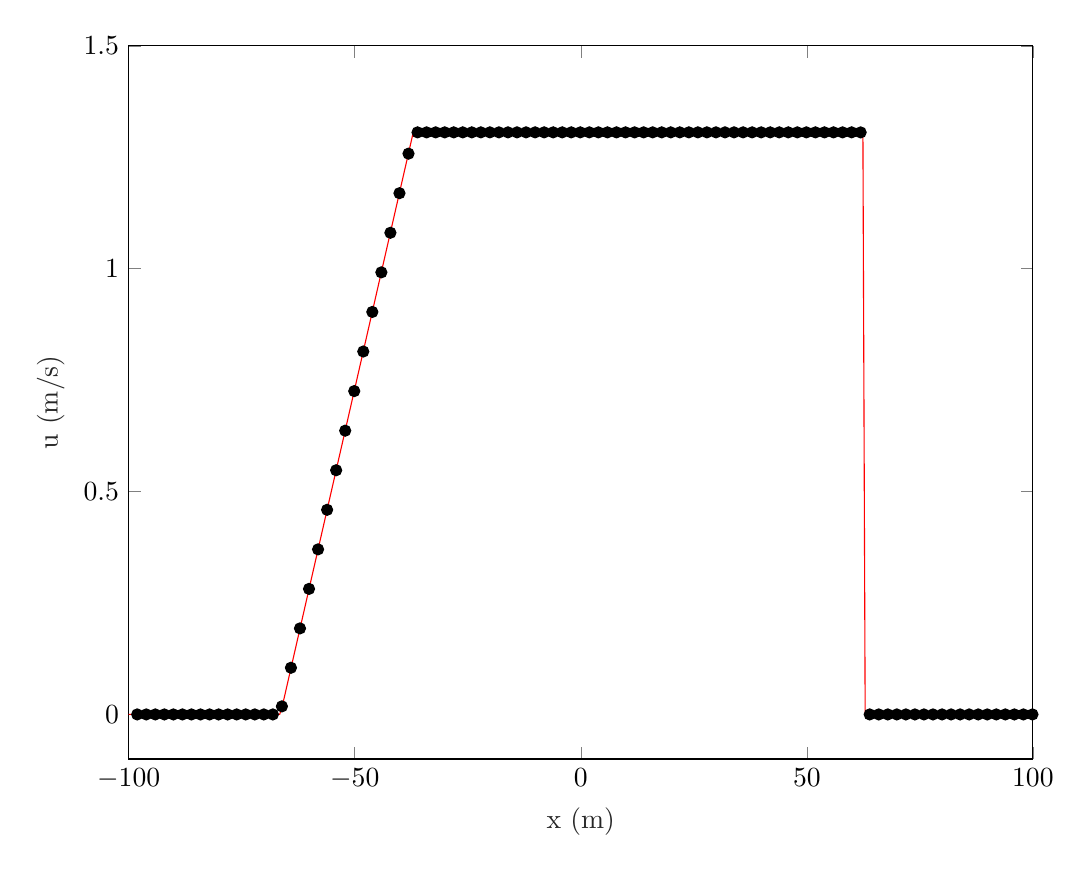
\begin{tikzpicture}

\begin{axis}[%
width=4.521in,
height=3.566in,
at={(0.758in,0.481in)},
scale only axis,
xmin=-100,
xmax=100,
xtick={-100,  -50,    0,   50,  100},
xlabel style={font=\color{white!15!black}},
xlabel={x (m)},
ymin=-0.1,
ymax=1.5,
ytick={  0, 0.5,   1, 1.5},
ylabel style={font=\color{white!15!black}},
ylabel={u (m/s)},
axis background/.style={fill=white}
]
\addplot [color=red, forget plot]
  table[row sep=crcr]{%
-100.1200120012	0\\
-99.6199619961996	0\\
-99.1199119911991	0\\
-98.6198619861986	0\\
-98.1198119811981	0\\
-97.6197619761976	0\\
-97.1197119711971	0\\
-96.6196619661966	0\\
-96.1196119611961	0\\
-95.6195619561956	0\\
-95.1195119511951	0\\
-94.6194619461946	0\\
-94.1194119411941	0\\
-93.6193619361936	0\\
-93.1193119311931	0\\
-92.6192619261926	0\\
-92.1192119211921	0\\
-91.6191619161916	0\\
-91.1191119111911	0\\
-90.6190619061906	0\\
-90.1190119011901	0\\
-89.6189618961896	0\\
-89.1189118911891	0\\
-88.6188618861886	0\\
-88.1188118811881	0\\
-87.6187618761876	0\\
-87.1187118711871	0\\
-86.6186618661866	0\\
-86.1186118611861	0\\
-85.6185618561856	0\\
-85.1185118511851	0\\
-84.6184618461846	0\\
-84.1184118411841	0\\
-83.6183618361836	0\\
-83.1183118311831	0\\
-82.6182618261826	0\\
-82.1182118211821	0\\
-81.6181618161816	0\\
-81.1181118111811	0\\
-80.6180618061806	0\\
-80.1180118011801	0\\
-79.6179617961796	0\\
-79.1179117911791	0\\
-78.6178617861786	0\\
-78.1178117811781	0\\
-77.6177617761776	0\\
-77.1177117711771	0\\
-76.6176617661766	0\\
-76.1176117611761	0\\
-75.6175617561756	0\\
-75.1175117511751	0\\
-74.6174617461746	0\\
-74.1174117411741	0\\
-73.6173617361736	0\\
-73.1173117311731	0\\
-72.6172617261726	0\\
-72.1172117211721	0\\
-71.6171617161716	0\\
-71.1171117111711	0\\
-70.6170617061706	0\\
-70.1170117011701	0\\
-69.6169616961696	0\\
-69.1169116911691	0\\
-68.6168616861686	0\\
-68.1168116811681	0\\
-67.6167616761676	0\\
-67.1167116711671	0\\
-66.6166616661666	0\\
-66.1166116611661	0.0146670427754891\\
-65.6165616561656	0.0368898348589196\\
-65.1165116511651	0.0591126269423506\\
-64.6164616461646	0.0813354190257805\\
-64.1164116411641	0.103558211109211\\
-63.6163616361636	0.125781003192642\\
-63.1163116311631	0.148003795276073\\
-62.6162616261626	0.170226587359503\\
-62.1162116211621	0.192449379442934\\
-61.6161616161616	0.214672171526364\\
-61.1161116111611	0.236894963609795\\
-60.6160616061606	0.259117755693226\\
-60.1160116011601	0.281340547776656\\
-59.6159615961596	0.303563339860087\\
-59.1159115911591	0.325786131943517\\
-58.6158615861586	0.348008924026948\\
-58.1158115811581	0.370231716110379\\
-57.6157615761576	0.392454508193809\\
-57.1157115711571	0.41467730027724\\
-56.6156615661566	0.43690009236067\\
-56.1156115611561	0.459122884444101\\
-55.6155615561556	0.481345676527531\\
-55.1155115511551	0.503568468610962\\
-54.6154615461546	0.525791260694392\\
-54.1154115411541	0.548014052777823\\
-53.6153615361536	0.570236844861254\\
-53.1153115311531	0.592459636944684\\
-52.6152615261526	0.614682429028115\\
-52.1152115211521	0.636905221111546\\
-51.6151615161516	0.659128013194976\\
-51.1151115111511	0.681350805278406\\
-50.6150615061506	0.703573597361837\\
-50.1150115011501	0.725796389445268\\
-49.6149614961496	0.748019181528698\\
-49.1149114911491	0.770241973612129\\
-48.6148614861486	0.792464765695559\\
-48.1148114811481	0.81468755777899\\
-47.6147614761476	0.836910349862421\\
-47.1147114711471	0.859133141945851\\
-46.6146614661466	0.881355934029282\\
-46.1146114611461	0.903578726112712\\
-45.6145614561456	0.925801518196143\\
-45.1145114511451	0.948024310279573\\
-44.6144614461446	0.970247102363004\\
-44.1144114411441	0.992469894446435\\
-43.6143614361436	1.01469268652987\\
-43.1143114311431	1.0369154786133\\
-42.6142614261426	1.05913827069673\\
-42.1142114211421	1.08136106278016\\
-41.6141614161416	1.10358385486359\\
-41.1141114111411	1.12580664694702\\
-40.6140614061406	1.14802943903045\\
-40.1140114011401	1.17025223111388\\
-39.6139613961396	1.19247502319731\\
-39.1139113911391	1.21469781528074\\
-38.6138613861386	1.23692060736417\\
-38.1138113811381	1.2591433994476\\
-37.6137613761376	1.28136619153103\\
-37.1137113711371	1.30358898361446\\
-36.6136613661366	1.30583375318171\\
-36.1136113611361	1.30583375318171\\
-35.6135613561356	1.30583375318171\\
-35.1135113511351	1.30583375318171\\
-34.6134613461346	1.30583375318171\\
-34.1134113411341	1.30583375318171\\
-33.6133613361336	1.30583375318171\\
-33.1133113311331	1.30583375318171\\
-32.6132613261326	1.30583375318171\\
-32.1132113211321	1.30583375318171\\
-31.6131613161316	1.30583375318171\\
-31.1131113111311	1.30583375318171\\
-30.6130613061306	1.30583375318171\\
-30.1130113011301	1.30583375318171\\
-29.6129612961296	1.30583375318171\\
-29.1129112911291	1.30583375318171\\
-28.6128612861286	1.30583375318171\\
-28.1128112811281	1.30583375318171\\
-27.6127612761276	1.30583375318171\\
-27.1127112711271	1.30583375318171\\
-26.6126612661266	1.30583375318171\\
-26.1126112611261	1.30583375318171\\
-25.6125612561256	1.30583375318171\\
-25.1125112511251	1.30583375318171\\
-24.6124612461246	1.30583375318171\\
-24.1124112411241	1.30583375318171\\
-23.6123612361236	1.30583375318171\\
-23.1123112311231	1.30583375318171\\
-22.6122612261226	1.30583375318171\\
-22.1122112211221	1.30583375318171\\
-21.6121612161216	1.30583375318171\\
-21.1121112111211	1.30583375318171\\
-20.6120612061206	1.30583375318171\\
-20.1120112011201	1.30583375318171\\
-19.6119611961196	1.30583375318171\\
-19.1119111911191	1.30583375318171\\
-18.6118611861186	1.30583375318171\\
-18.1118111811181	1.30583375318171\\
-17.6117611761176	1.30583375318171\\
-17.1117111711171	1.30583375318171\\
-16.6116611661166	1.30583375318171\\
-16.1116111611161	1.30583375318171\\
-15.6115611561156	1.30583375318171\\
-15.1115111511151	1.30583375318171\\
-14.6114611461146	1.30583375318171\\
-14.1114111411141	1.30583375318171\\
-13.6113611361136	1.30583375318171\\
-13.1113111311131	1.30583375318171\\
-12.6112611261126	1.30583375318171\\
-12.1112111211121	1.30583375318171\\
-11.6111611161116	1.30583375318171\\
-11.1111111111111	1.30583375318171\\
-10.6110611061106	1.30583375318171\\
-10.1110111011101	1.30583375318171\\
-9.61096109610961	1.30583375318171\\
-9.1109110911091	1.30583375318171\\
-8.61086108610861	1.30583375318171\\
-8.11081108110811	1.30583375318171\\
-7.61076107610761	1.30583375318171\\
-7.1107110711071	1.30583375318171\\
-6.6106610661066	1.30583375318171\\
-6.11061106110611	1.30583375318171\\
-5.61056105610561	1.30583375318171\\
-5.11051105110511	1.30583375318171\\
-4.6104610461046	1.30583375318171\\
-4.1104110411041	1.30583375318171\\
-3.61036103610361	1.30583375318171\\
-3.11031103110311	1.30583375318171\\
-2.61026102610261	1.30583375318171\\
-2.1102110211021	1.30583375318171\\
-1.6101610161016	1.30583375318171\\
-1.11011101110111	1.30583375318171\\
-0.610061006100608	1.30583375318171\\
-0.110011001100105	1.30583375318171\\
0.390039003900398	1.30583375318171\\
0.890089008900901	1.30583375318171\\
1.39013901390139	1.30583375318171\\
1.89018901890189	1.30583375318171\\
2.3902390239024	1.30583375318171\\
2.8902890289029	1.30583375318171\\
3.3903390339034	1.30583375318171\\
3.89038903890389	1.30583375318171\\
4.39043904390439	1.30583375318171\\
4.8904890489049	1.30583375318171\\
5.3905390539054	1.30583375318171\\
5.8905890589059	1.30583375318171\\
6.39063906390639	1.30583375318171\\
6.89068906890689	1.30583375318171\\
7.3907390739074	1.30583375318171\\
7.8907890789079	1.30583375318171\\
8.39083908390839	1.30583375318171\\
8.89088908890889	1.30583375318171\\
9.3909390939094	1.30583375318171\\
9.8909890989099	1.30583375318171\\
10.3910391039104	1.30583375318171\\
10.8910891089109	1.30583375318171\\
11.3911391139114	1.30583375318171\\
11.8911891189119	1.30583375318171\\
12.3912391239124	1.30583375318171\\
12.8912891289129	1.30583375318171\\
13.3913391339134	1.30583375318171\\
13.8913891389139	1.30583375318171\\
14.3914391439144	1.30583375318171\\
14.8914891489149	1.30583375318171\\
15.3915391539154	1.30583375318171\\
15.8915891589159	1.30583375318171\\
16.3916391639164	1.30583375318171\\
16.8916891689169	1.30583375318171\\
17.3917391739174	1.30583375318171\\
17.8917891789179	1.30583375318171\\
18.3918391839184	1.30583375318171\\
18.8918891889189	1.30583375318171\\
19.3919391939194	1.30583375318171\\
19.8919891989199	1.30583375318171\\
20.3920392039204	1.30583375318171\\
20.8920892089209	1.30583375318171\\
21.3921392139214	1.30583375318171\\
21.8921892189219	1.30583375318171\\
22.3922392239224	1.30583375318171\\
22.8922892289229	1.30583375318171\\
23.3923392339234	1.30583375318171\\
23.8923892389239	1.30583375318171\\
24.3924392439244	1.30583375318171\\
24.8924892489249	1.30583375318171\\
25.3925392539254	1.30583375318171\\
25.8925892589259	1.30583375318171\\
26.3926392639264	1.30583375318171\\
26.8926892689269	1.30583375318171\\
27.3927392739274	1.30583375318171\\
27.8927892789279	1.30583375318171\\
28.3928392839284	1.30583375318171\\
28.8928892889289	1.30583375318171\\
29.3929392939294	1.30583375318171\\
29.8929892989299	1.30583375318171\\
30.3930393039304	1.30583375318171\\
30.8930893089309	1.30583375318171\\
31.3931393139314	1.30583375318171\\
31.8931893189319	1.30583375318171\\
32.3932393239324	1.30583375318171\\
32.8932893289329	1.30583375318171\\
33.3933393339334	1.30583375318171\\
33.8933893389339	1.30583375318171\\
34.3934393439344	1.30583375318171\\
34.8934893489349	1.30583375318171\\
35.3935393539354	1.30583375318171\\
35.8935893589359	1.30583375318171\\
36.3936393639364	1.30583375318171\\
36.8936893689369	1.30583375318171\\
37.3937393739374	1.30583375318171\\
37.8937893789379	1.30583375318171\\
38.3938393839384	1.30583375318171\\
38.8938893889389	1.30583375318171\\
39.3939393939394	1.30583375318171\\
39.8939893989399	1.30583375318171\\
40.3940394039404	1.30583375318171\\
40.8940894089409	1.30583375318171\\
41.3941394139414	1.30583375318171\\
41.8941894189419	1.30583375318171\\
42.3942394239424	1.30583375318171\\
42.8942894289429	1.30583375318171\\
43.3943394339434	1.30583375318171\\
43.8943894389439	1.30583375318171\\
44.3944394439444	1.30583375318171\\
44.8944894489449	1.30583375318171\\
45.3945394539454	1.30583375318171\\
45.8945894589459	1.30583375318171\\
46.3946394639464	1.30583375318171\\
46.8946894689469	1.30583375318171\\
47.3947394739474	1.30583375318171\\
47.8947894789479	1.30583375318171\\
48.3948394839484	1.30583375318171\\
48.8948894889489	1.30583375318171\\
49.3949394939494	1.30583375318171\\
49.8949894989499	1.30583375318171\\
50.3950395039504	1.30583375318171\\
50.8950895089509	1.30583375318171\\
51.3951395139514	1.30583375318171\\
51.8951895189519	1.30583375318171\\
52.3952395239524	1.30583375318171\\
52.8952895289529	1.30583375318171\\
53.3953395339534	1.30583375318171\\
53.8953895389539	1.30583375318171\\
54.3954395439544	1.30583375318171\\
54.8954895489549	1.30583375318171\\
55.3955395539554	1.30583375318171\\
55.8955895589559	1.30583375318171\\
56.3956395639564	1.30583375318171\\
56.8956895689569	1.30583375318171\\
57.3957395739574	1.30583375318171\\
57.8957895789579	1.30583375318171\\
58.3958395839584	1.30583375318171\\
58.8958895889589	1.30583375318171\\
59.3959395939594	1.30583375318171\\
59.8959895989599	1.30583375318171\\
60.3960396039604	1.30583375318171\\
60.8960896089609	1.30583375318171\\
61.3961396139614	1.30583375318171\\
61.8961896189619	1.30583375318171\\
62.3962396239624	1.30583375318171\\
62.8962896289629	0\\
63.3963396339634	0\\
63.8963896389639	0\\
64.3964396439644	0\\
64.8964896489649	0\\
65.3965396539654	0\\
65.8965896589659	0\\
66.3966396639664	0\\
66.8966896689669	0\\
67.3967396739674	0\\
67.8967896789679	0\\
68.3968396839684	0\\
68.8968896889689	0\\
69.3969396939694	0\\
69.8969896989699	0\\
70.3970397039704	0\\
70.8970897089709	0\\
71.3971397139714	0\\
71.8971897189719	0\\
72.3972397239724	0\\
72.8972897289729	0\\
73.3973397339734	0\\
73.8973897389739	0\\
74.3974397439744	0\\
74.8974897489749	0\\
75.3975397539754	0\\
75.8975897589759	0\\
76.3976397639764	0\\
76.8976897689769	0\\
77.3977397739774	0\\
77.8977897789779	0\\
78.3978397839784	0\\
78.8978897889789	0\\
79.3979397939794	0\\
79.8979897989799	0\\
80.3980398039804	0\\
80.8980898089809	0\\
81.3981398139814	0\\
81.8981898189819	0\\
82.3982398239824	0\\
82.8982898289829	0\\
83.3983398339834	0\\
83.8983898389839	0\\
84.3984398439844	0\\
84.8984898489849	0\\
85.3985398539854	0\\
85.8985898589859	0\\
86.3986398639864	0\\
86.8986898689869	0\\
87.3987398739874	0\\
87.8987898789879	0\\
88.3988398839884	0\\
88.8988898889889	0\\
89.3989398939894	0\\
89.8989898989899	0\\
90.3990399039904	0\\
90.8990899089909	0\\
91.3991399139914	0\\
91.8991899189919	0\\
92.3992399239924	0\\
92.8992899289929	0\\
93.3993399339934	0\\
93.8993899389939	0\\
94.3994399439944	0\\
94.8994899489949	0\\
95.3995399539954	0\\
95.8995899589959	0\\
96.3996399639964	0\\
96.8996899689969	0\\
97.3997399739974	0\\
97.8997899789979	0\\
98.3998399839984	0\\
98.8998899889989	0\\
99.3999399939994	0\\
99.8999899989999	0\\
};
\addplot [color=black, draw=none, mark=*, mark options={solid, black}, forget plot]
  table[row sep=crcr]{%
-100.1200120012	0\\
-98.1198119811981	0\\
-96.1196119611961	0\\
-94.1194119411941	0\\
-92.1192119211921	0\\
-90.1190119011901	0\\
-88.1188118811881	0\\
-86.1186118611861	0\\
-84.1184118411841	0\\
-82.1182118211821	0\\
-80.1180118011801	0\\
-78.1178117811781	0\\
-76.1176117611761	0\\
-74.1174117411741	0\\
-72.1172117211721	0\\
-70.1170117011701	0\\
-68.1168116811681	0\\
-66.1166116611661	0.018067543417192\\
-64.1164116411641	0.104704068951157\\
-62.1162116211621	0.193039259866322\\
-60.1160116011601	0.281629405650236\\
-58.1158115811581	0.370315437964994\\
-56.1156115611561	0.459049156770148\\
-54.1154115411541	0.547810159661504\\
-52.1152115211521	0.636588029347613\\
-50.1150115011501	0.725376666195332\\
-48.1148114811481	0.814171969830254\\
-46.1146114611461	0.90297060329279\\
-44.1144114411441	0.991768949673571\\
-42.1142114211421	1.08056139131135\\
-40.1140114011401	1.16933511491941\\
-38.1138113811381	1.25804367128075\\
-36.1136113611361	1.30584984995419\\
-34.1134113411341	1.30582514646683\\
-32.1132113211321	1.30583042509924\\
-30.1130113011301	1.30583205851541\\
-28.1128112811281	1.30583274350332\\
-26.1126112611261	1.30583304174086\\
-24.1124112411241	1.30583315346163\\
-22.1122112211221	1.30583340848299\\
-20.1120112011201	1.30583351983945\\
-18.1118111811181	1.30583346763977\\
-16.1116111611161	1.30583351724206\\
-14.1114111411141	1.30583352251971\\
-12.1112111211121	1.30583368954523\\
-10.1110111011101	1.30583370493342\\
-8.11081108110811	1.30583352278156\\
-6.11061106110611	1.30583359394613\\
-4.1104110411041	1.30583377074515\\
-2.1102110211021	1.30583370987723\\
-0.110011001100105	1.30583363755937\\
1.89018901890189	1.30583358307652\\
3.89038903890389	1.30583362969097\\
5.8905890589059	1.30583385913076\\
7.8907890789079	1.30583370865049\\
9.8909890989099	1.30583351935089\\
11.8911891189119	1.30583374510096\\
13.8913891389139	1.30583381632435\\
15.8915891589159	1.30583377789548\\
17.8917891789179	1.30583367639496\\
19.8919891989199	1.30583339704962\\
21.8921892189219	1.30583387447456\\
23.8923892389239	1.30583405228227\\
25.8925892589259	1.30583347381001\\
27.8927892789279	1.30583347715004\\
29.8929892989299	1.30583375435938\\
31.8931893189319	1.30583388661588\\
33.8933893389339	1.3058341444873\\
35.8935893589359	1.3058331973405\\
37.8937893789379	1.30583329405526\\
39.8939893989399	1.30583423642182\\
41.8941894189419	1.30583408352188\\
43.8943894389439	1.30583332068146\\
45.8945894589459	1.30583350247617\\
47.8947894789479	1.30583345096515\\
49.8949894989499	1.3058343866342\\
51.8951895189519	1.30583444059326\\
53.8953895389539	1.30582936999627\\
55.8955895589559	1.30584066757646\\
57.8957895789579	1.30581747770344\\
59.8959895989599	1.30587629949119\\
61.8961896189619	1.305743078258\\
63.8963896389639	0\\
65.8965896589659	0\\
67.8967896789679	0\\
69.8969896989699	0\\
71.8971897189719	0\\
73.8973897389739	0\\
75.8975897589759	0\\
77.8977897789779	0\\
79.8979897989799	0\\
81.8981898189819	0\\
83.8983898389839	0\\
85.8985898589859	0\\
87.8987898789879	0\\
89.8989898989899	0\\
91.8991899189919	0\\
93.8993899389939	0\\
95.8995899589959	0\\
97.8997899789979	0\\
99.8999899989999	0\\
};
\end{axis}
\end{tikzpicture}%
		\caption{$u$}
	\end{subfigure}
	\begin{subfigure}{0.49\textwidth}
		\centering
		% This file was created by matlab2tikz.
%
%The latest updates can be retrieved from
%  http://www.mathworks.com/matlabcentral/fileexchange/22022-matlab2tikz-matlab2tikz
%where you can also make suggestions and rate matlab2tikz.
%
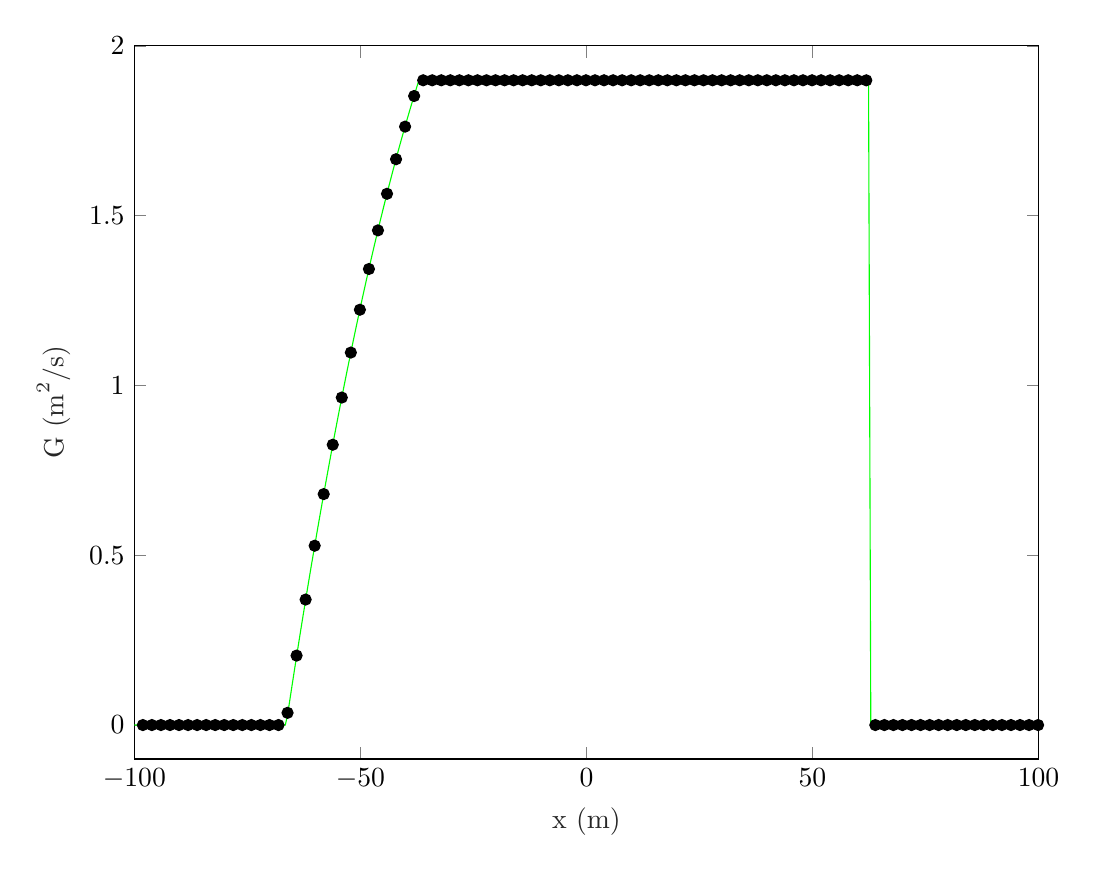
\begin{tikzpicture}

\begin{axis}[%
width=4.521in,
height=3.566in,
at={(0.758in,0.481in)},
scale only axis,
xmin=-100,
xmax=100,
xtick={-100,  -50,    0,   50,  100},
xlabel style={font=\color{white!15!black}},
xlabel={x (m)},
ymin=-0.1,
ymax=2,
ytick={  0, 0.5,   1, 1.5,   2},
ylabel style={font=\color{white!15!black}},
ylabel={$\text{G (m}^\text{2}\text{/s)}$},
axis background/.style={fill=white}
]
\addplot [color=green, forget plot]
  table[row sep=crcr]{%
-100.1200120012	0\\
-99.6199619961996	0\\
-99.1199119911991	0\\
-98.6198619861986	0\\
-98.1198119811981	0\\
-97.6197619761976	0\\
-97.1197119711971	0\\
-96.6196619661966	0\\
-96.1196119611961	0\\
-95.6195619561956	0\\
-95.1195119511951	0\\
-94.6194619461946	0\\
-94.1194119411941	0\\
-93.6193619361936	0\\
-93.1193119311931	0\\
-92.6192619261926	0\\
-92.1192119211921	0\\
-91.6191619161916	0\\
-91.1191119111911	0\\
-90.6190619061906	0\\
-90.1190119011901	0\\
-89.6189618961896	0\\
-89.1189118911891	0\\
-88.6188618861886	0\\
-88.1188118811881	0\\
-87.6187618761876	0\\
-87.1187118711871	0\\
-86.6186618661866	0\\
-86.1186118611861	0\\
-85.6185618561856	0\\
-85.1185118511851	0\\
-84.6184618461846	0\\
-84.1184118411841	0\\
-83.6183618361836	0\\
-83.1183118311831	0\\
-82.6182618261826	0\\
-82.1182118211821	0\\
-81.6181618161816	0\\
-81.1181118111811	0\\
-80.6180618061806	0\\
-80.1180118011801	0\\
-79.6179617961796	0\\
-79.1179117911791	0\\
-78.6178617861786	0\\
-78.1178117811781	0\\
-77.6177617761776	0\\
-77.1177117711771	0\\
-76.6176617661766	0\\
-76.1176117611761	0\\
-75.6175617561756	0\\
-75.1175117511751	0\\
-74.6174617461746	0\\
-74.1174117411741	0\\
-73.6173617361736	0\\
-73.1173117311731	0\\
-72.6172617261726	0\\
-72.1172117211721	0\\
-71.6171617161716	0\\
-71.1171117111711	0\\
-70.6170617061706	0\\
-70.1170117011701	0\\
-69.6169616961696	0\\
-69.1169116911691	0\\
-68.6168616861686	0\\
-68.1168116811681	0\\
-67.6167616761676	0\\
-67.1167116711671	0\\
-66.6166616661666	0\\
-66.1166116611661	0.029237033225255\\
-65.6165616561656	0.0731664886489198\\
-65.1165116511651	0.116652757573435\\
-64.6164616461646	0.159697518099892\\
-64.1164116411641	0.20230244832939\\
-63.6163616361636	0.244469226363021\\
-63.1163116311631	0.286199530301882\\
-62.6162616261626	0.327495038247065\\
-62.1162116211621	0.368357428299667\\
-61.6161616161616	0.408788378560781\\
-61.1161116111611	0.448789567131504\\
-60.6160616061606	0.488362672112931\\
-60.1160116011601	0.527509371606154\\
-59.6159615961596	0.56623134371227\\
-59.1159115911591	0.604530266532375\\
-58.6158615861586	0.64240781816756\\
-58.1158115811581	0.679865676718924\\
-57.6157615761576	0.716905520287559\\
-57.1157115711571	0.753529026974562\\
-56.6156615661566	0.789737874881026\\
-56.1156115611561	0.825533742108047\\
-55.6155615561556	0.860918306756719\\
-55.1155115511551	0.895893246928137\\
-54.6154615461546	0.930460240723397\\
-54.1154115411541	0.964620966243593\\
-53.6153615361536	0.998377101589819\\
-53.1153115311531	1.03173032486317\\
-52.6152615261526	1.06468231416474\\
-52.1152115211521	1.09723474759563\\
-51.6151615161516	1.12938930325693\\
-51.1151115111511	1.16114765924973\\
-50.6150615061506	1.19251149367514\\
-50.1150115011501	1.22348248463424\\
-49.6149614961496	1.25406231022812\\
-49.1149114911491	1.2842526485579\\
-48.6148614861486	1.31405517772465\\
-48.1148114811481	1.34347157582948\\
-47.6147614761476	1.37250352097347\\
-47.1147114711471	1.40115269125773\\
-46.6146614661466	1.42942076478335\\
-46.1146114611461	1.45730941965142\\
-45.6145614561456	1.48482033396304\\
-45.1145114511451	1.51195518581931\\
-44.6144614461446	1.53871565332131\\
-44.1144114411441	1.56510341457014\\
-43.6143614361436	1.59112014766691\\
-43.1143114311431	1.61676753071269\\
-42.6142614261426	1.6420472418086\\
-42.1142114211421	1.66696095905571\\
-41.6141614161416	1.69151036055513\\
-41.1141114111411	1.71569712440796\\
-40.6140614061406	1.73952292871528\\
-40.1140114011401	1.7629894515782\\
-39.6139613961396	1.7860983710978\\
-39.1139113911391	1.80885136537518\\
-38.6138613861386	1.83125011251144\\
-38.1138113811381	1.85329629060767\\
-37.6137613761376	1.87499157776497\\
-37.1137113711371	1.89633765208443\\
-36.6136613661366	1.89847450901855\\
-36.1136113611361	1.89847450901855\\
-35.6135613561356	1.89847450901855\\
-35.1135113511351	1.89847450901855\\
-34.6134613461346	1.89847450901855\\
-34.1134113411341	1.89847450901855\\
-33.6133613361336	1.89847450901855\\
-33.1133113311331	1.89847450901855\\
-32.6132613261326	1.89847450901855\\
-32.1132113211321	1.89847450901855\\
-31.6131613161316	1.89847450901855\\
-31.1131113111311	1.89847450901855\\
-30.6130613061306	1.89847450901855\\
-30.1130113011301	1.89847450901855\\
-29.6129612961296	1.89847450901855\\
-29.1129112911291	1.89847450901855\\
-28.6128612861286	1.89847450901855\\
-28.1128112811281	1.89847450901855\\
-27.6127612761276	1.89847450901855\\
-27.1127112711271	1.89847450901855\\
-26.6126612661266	1.89847450901855\\
-26.1126112611261	1.89847450901855\\
-25.6125612561256	1.89847450901855\\
-25.1125112511251	1.89847450901855\\
-24.6124612461246	1.89847450901855\\
-24.1124112411241	1.89847450901855\\
-23.6123612361236	1.89847450901855\\
-23.1123112311231	1.89847450901855\\
-22.6122612261226	1.89847450901855\\
-22.1122112211221	1.89847450901855\\
-21.6121612161216	1.89847450901855\\
-21.1121112111211	1.89847450901855\\
-20.6120612061206	1.89847450901855\\
-20.1120112011201	1.89847450901855\\
-19.6119611961196	1.89847450901855\\
-19.1119111911191	1.89847450901855\\
-18.6118611861186	1.89847450901855\\
-18.1118111811181	1.89847450901855\\
-17.6117611761176	1.89847450901855\\
-17.1117111711171	1.89847450901855\\
-16.6116611661166	1.89847450901855\\
-16.1116111611161	1.89847450901855\\
-15.6115611561156	1.89847450901855\\
-15.1115111511151	1.89847450901855\\
-14.6114611461146	1.89847450901855\\
-14.1114111411141	1.89847450901855\\
-13.6113611361136	1.89847450901855\\
-13.1113111311131	1.89847450901855\\
-12.6112611261126	1.89847450901855\\
-12.1112111211121	1.89847450901855\\
-11.6111611161116	1.89847450901855\\
-11.1111111111111	1.89847450901855\\
-10.6110611061106	1.89847450901855\\
-10.1110111011101	1.89847450901855\\
-9.61096109610961	1.89847450901855\\
-9.1109110911091	1.89847450901855\\
-8.61086108610861	1.89847450901855\\
-8.11081108110811	1.89847450901855\\
-7.61076107610761	1.89847450901855\\
-7.1107110711071	1.89847450901855\\
-6.6106610661066	1.89847450901855\\
-6.11061106110611	1.89847450901855\\
-5.61056105610561	1.89847450901855\\
-5.11051105110511	1.89847450901855\\
-4.6104610461046	1.89847450901855\\
-4.1104110411041	1.89847450901855\\
-3.61036103610361	1.89847450901855\\
-3.11031103110311	1.89847450901855\\
-2.61026102610261	1.89847450901855\\
-2.1102110211021	1.89847450901855\\
-1.6101610161016	1.89847450901855\\
-1.11011101110111	1.89847450901855\\
-0.610061006100608	1.89847450901855\\
-0.110011001100105	1.89847450901855\\
0.390039003900398	1.89847450901855\\
0.890089008900901	1.89847450901855\\
1.39013901390139	1.89847450901855\\
1.89018901890189	1.89847450901855\\
2.3902390239024	1.89847450901855\\
2.8902890289029	1.89847450901855\\
3.3903390339034	1.89847450901855\\
3.89038903890389	1.89847450901855\\
4.39043904390439	1.89847450901855\\
4.8904890489049	1.89847450901855\\
5.3905390539054	1.89847450901855\\
5.8905890589059	1.89847450901855\\
6.39063906390639	1.89847450901855\\
6.89068906890689	1.89847450901855\\
7.3907390739074	1.89847450901855\\
7.8907890789079	1.89847450901855\\
8.39083908390839	1.89847450901855\\
8.89088908890889	1.89847450901855\\
9.3909390939094	1.89847450901855\\
9.8909890989099	1.89847450901855\\
10.3910391039104	1.89847450901855\\
10.8910891089109	1.89847450901855\\
11.3911391139114	1.89847450901855\\
11.8911891189119	1.89847450901855\\
12.3912391239124	1.89847450901855\\
12.8912891289129	1.89847450901855\\
13.3913391339134	1.89847450901855\\
13.8913891389139	1.89847450901855\\
14.3914391439144	1.89847450901855\\
14.8914891489149	1.89847450901855\\
15.3915391539154	1.89847450901855\\
15.8915891589159	1.89847450901855\\
16.3916391639164	1.89847450901855\\
16.8916891689169	1.89847450901855\\
17.3917391739174	1.89847450901855\\
17.8917891789179	1.89847450901855\\
18.3918391839184	1.89847450901855\\
18.8918891889189	1.89847450901855\\
19.3919391939194	1.89847450901855\\
19.8919891989199	1.89847450901855\\
20.3920392039204	1.89847450901855\\
20.8920892089209	1.89847450901855\\
21.3921392139214	1.89847450901855\\
21.8921892189219	1.89847450901855\\
22.3922392239224	1.89847450901855\\
22.8922892289229	1.89847450901855\\
23.3923392339234	1.89847450901855\\
23.8923892389239	1.89847450901855\\
24.3924392439244	1.89847450901855\\
24.8924892489249	1.89847450901855\\
25.3925392539254	1.89847450901855\\
25.8925892589259	1.89847450901855\\
26.3926392639264	1.89847450901855\\
26.8926892689269	1.89847450901855\\
27.3927392739274	1.89847450901855\\
27.8927892789279	1.89847450901855\\
28.3928392839284	1.89847450901855\\
28.8928892889289	1.89847450901855\\
29.3929392939294	1.89847450901855\\
29.8929892989299	1.89847450901855\\
30.3930393039304	1.89847450901855\\
30.8930893089309	1.89847450901855\\
31.3931393139314	1.89847450901855\\
31.8931893189319	1.89847450901855\\
32.3932393239324	1.89847450901855\\
32.8932893289329	1.89847450901855\\
33.3933393339334	1.89847450901855\\
33.8933893389339	1.89847450901855\\
34.3934393439344	1.89847450901855\\
34.8934893489349	1.89847450901855\\
35.3935393539354	1.89847450901855\\
35.8935893589359	1.89847450901855\\
36.3936393639364	1.89847450901855\\
36.8936893689369	1.89847450901855\\
37.3937393739374	1.89847450901855\\
37.8937893789379	1.89847450901855\\
38.3938393839384	1.89847450901855\\
38.8938893889389	1.89847450901855\\
39.3939393939394	1.89847450901855\\
39.8939893989399	1.89847450901855\\
40.3940394039404	1.89847450901855\\
40.8940894089409	1.89847450901855\\
41.3941394139414	1.89847450901855\\
41.8941894189419	1.89847450901855\\
42.3942394239424	1.89847450901855\\
42.8942894289429	1.89847450901855\\
43.3943394339434	1.89847450901855\\
43.8943894389439	1.89847450901855\\
44.3944394439444	1.89847450901855\\
44.8944894489449	1.89847450901855\\
45.3945394539454	1.89847450901855\\
45.8945894589459	1.89847450901855\\
46.3946394639464	1.89847450901855\\
46.8946894689469	1.89847450901855\\
47.3947394739474	1.89847450901855\\
47.8947894789479	1.89847450901855\\
48.3948394839484	1.89847450901855\\
48.8948894889489	1.89847450901855\\
49.3949394939494	1.89847450901855\\
49.8949894989499	1.89847450901855\\
50.3950395039504	1.89847450901855\\
50.8950895089509	1.89847450901855\\
51.3951395139514	1.89847450901855\\
51.8951895189519	1.89847450901855\\
52.3952395239524	1.89847450901855\\
52.8952895289529	1.89847450901855\\
53.3953395339534	1.89847450901855\\
53.8953895389539	1.89847450901855\\
54.3954395439544	1.89847450901855\\
54.8954895489549	1.89847450901855\\
55.3955395539554	1.89847450901855\\
55.8955895589559	1.89847450901855\\
56.3956395639564	1.89847450901855\\
56.8956895689569	1.89847450901855\\
57.3957395739574	1.89847450901855\\
57.8957895789579	1.89847450901855\\
58.3958395839584	1.89847450901855\\
58.8958895889589	1.89847450901855\\
59.3959395939594	1.89847450901855\\
59.8959895989599	1.89847450901855\\
60.3960396039604	1.89847450901855\\
60.8960896089609	1.89847450901855\\
61.3961396139614	1.89847450901855\\
61.8961896189619	1.89847450901855\\
62.3962396239624	1.89847450901855\\
62.8962896289629	0\\
63.3963396339634	0\\
63.8963896389639	0\\
64.3964396439644	0\\
64.8964896489649	0\\
65.3965396539654	0\\
65.8965896589659	0\\
66.3966396639664	0\\
66.8966896689669	0\\
67.3967396739674	0\\
67.8967896789679	0\\
68.3968396839684	0\\
68.8968896889689	0\\
69.3969396939694	0\\
69.8969896989699	0\\
70.3970397039704	0\\
70.8970897089709	0\\
71.3971397139714	0\\
71.8971897189719	0\\
72.3972397239724	0\\
72.8972897289729	0\\
73.3973397339734	0\\
73.8973897389739	0\\
74.3974397439744	0\\
74.8974897489749	0\\
75.3975397539754	0\\
75.8975897589759	0\\
76.3976397639764	0\\
76.8976897689769	0\\
77.3977397739774	0\\
77.8977897789779	0\\
78.3978397839784	0\\
78.8978897889789	0\\
79.3979397939794	0\\
79.8979897989799	0\\
80.3980398039804	0\\
80.8980898089809	0\\
81.3981398139814	0\\
81.8981898189819	0\\
82.3982398239824	0\\
82.8982898289829	0\\
83.3983398339834	0\\
83.8983898389839	0\\
84.3984398439844	0\\
84.8984898489849	0\\
85.3985398539854	0\\
85.8985898589859	0\\
86.3986398639864	0\\
86.8986898689869	0\\
87.3987398739874	0\\
87.8987898789879	0\\
88.3988398839884	0\\
88.8988898889889	0\\
89.3989398939894	0\\
89.8989898989899	0\\
90.3990399039904	0\\
90.8990899089909	0\\
91.3991399139914	0\\
91.8991899189919	0\\
92.3992399239924	0\\
92.8992899289929	0\\
93.3993399339934	0\\
93.8993899389939	0\\
94.3994399439944	0\\
94.8994899489949	0\\
95.3995399539954	0\\
95.8995899589959	0\\
96.3996399639964	0\\
96.8996899689969	0\\
97.3997399739974	0\\
97.8997899789979	0\\
98.3998399839984	0\\
98.8998899889989	0\\
99.3999399939994	0\\
99.8999899989999	0\\
};
\addplot [color=black, draw=none, mark=*, mark options={solid, black}, forget plot]
  table[row sep=crcr]{%
-100.1200120012	0\\
-98.1198119811981	0\\
-96.1196119611961	0\\
-94.1194119411941	0\\
-92.1192119211921	0\\
-90.1190119011901	0\\
-88.1188118811881	0\\
-86.1186118611861	0\\
-84.1184118411841	0\\
-82.1182118211821	0\\
-80.1180118011801	0\\
-78.1178117811781	0\\
-76.1176117611761	0\\
-74.1174117411741	0\\
-72.1172117211721	0\\
-70.1170117011701	0\\
-68.1168116811681	0\\
-66.1166116611661	0.0359878394766163\\
-64.1164116411641	0.204487360948335\\
-62.1162116211621	0.369436188861586\\
-60.1160116011601	0.528015407278974\\
-58.1158115811581	0.680005998502211\\
-56.1156115611561	0.825415658214476\\
-54.1154115411541	0.964309377118333\\
-52.1152115211521	1.09677291220492\\
-50.1150115011501	1.22290115285691\\
-48.1148114811481	1.34279344122832\\
-46.1146114611461	1.45655127320249\\
-44.1144114411441	1.56427676095913\\
-42.1142114211421	1.66607076970514\\
-40.1140114011401	1.76202807666687\\
-38.1138113811381	1.85221355115646\\
-36.1136113611361	1.8984899064546\\
-34.1134113411341	1.89846630582009\\
-32.1132113211321	1.89847133729114\\
-30.1130113011301	1.89847288810496\\
-28.1128112811281	1.89847354367228\\
-26.1126112611261	1.89847382568126\\
-24.1124112411241	1.89847393238489\\
-22.1122112211221	1.89847416873701\\
-20.1120112011201	1.89847427749689\\
-18.1118111811181	1.89847422477676\\
-16.1116111611161	1.89847427618055\\
-14.1114111411141	1.89847427872353\\
-12.1112111211121	1.89847443986087\\
-10.1110111011101	1.89847445337099\\
-8.11081108110811	1.89847427383913\\
-6.11061106110611	1.89847434338401\\
-4.1104110411041	1.89847451448365\\
-2.1102110211021	1.89847445910864\\
-0.110011001100105	1.89847438319536\\
1.89018901890189	1.89847433354248\\
3.89038903890389	1.89847437030492\\
5.8905890589059	1.89847459152836\\
7.8907890789079	1.89847444918848\\
9.8909890989099	1.89847426673864\\
11.8911891189119	1.89847449090853\\
13.8913891389139	1.89847455990236\\
15.8915891589159	1.89847451667242\\
17.8917891789179	1.89847440764947\\
19.8919891989199	1.89847413572053\\
21.8921892189219	1.89847459387426\\
23.8923892389239	1.89847475297666\\
25.8925892589259	1.89847418534422\\
27.8927892789279	1.89847421691468\\
29.8929892989299	1.89847445789456\\
31.8931893189319	1.8984745982811\\
33.8933893389339	1.89847485489723\\
35.8935893589359	1.89847395283797\\
37.8937893789379	1.89847403254209\\
39.8939893989399	1.8984749266389\\
41.8941894189419	1.89847479309058\\
43.8943894389439	1.89847403973737\\
45.8945894589459	1.89847419530322\\
47.8947894789479	1.89847414530057\\
49.8949894989499	1.89847502439602\\
51.8951895189519	1.89847504016845\\
53.8953895389539	1.89847015555343\\
55.8955895589559	1.89848094063038\\
57.8957895789579	1.89845878335127\\
59.8959895989599	1.89851496911976\\
61.8961896189619	1.89838638948092\\
63.8963896389639	0\\
65.8965896589659	0\\
67.8967896789679	0\\
69.8969896989699	0\\
71.8971897189719	0\\
73.8973897389739	0\\
75.8975897589759	0\\
77.8977897789779	0\\
79.8979897989799	0\\
81.8981898189819	0\\
83.8983898389839	0\\
85.8985898589859	0\\
87.8987898789879	0\\
89.8989898989899	0\\
91.8991899189919	0\\
93.8993899389939	0\\
95.8995899589959	0\\
97.8997899789979	0\\
99.8999899989999	0\\
};
\end{axis}
\end{tikzpicture}%
		\caption{$G$}
	\end{subfigure}
	\caption{Numerical Solution}
\end{figure}
\begin{table}
\begin{tabular}{c c c c c}
Context	 & $h$ & $G$ & $uh$ & $\mathcal{H}$ \\
\hline
Initial	& $300.032154872864$ & $0$ & $0$ & $2452.77542969807$ \\
End	& $300.03215487288$ & $220.741414068836$ & $220.741410229554$ & $2442.82816385916$ \\
Analytic Flux & $0$ & $220.741414068868$& $220.741414068868$ & $0$ \\
Conservation Error &  $5.342708725849857 \times 10^{-14}$ & $3.200284481863491\times 10^{-11}$ 
 & $3.839314018705409\times 10^{-6}$ & $0.004055514303702256$
\end{tabular}
\caption{Conservation error for gSGN solver dam-break solution}
\end{table}


\subsection{Numerical Experiments}

\subsubsection{Smooth Dambreak}

\begin{align}
h(x,0) & = h_0 + \dfrac{h_1 - h_0}{2} \left(1 + \tanh\left(\dfrac{x}{\alpha}\right)\right)  \\
u(x,0) &= 0 \\
G(x,0) &= 0
\end{align}

$\alpha = 2$

\begin{figure}
	\tikzset{every picture/.style={scale=0.75}}%
	\centering
	\begin{subfigure}{0.49\textwidth}
		\centering
		% This file was created by matlab2tikz.
%
%The latest updates can be retrieved from
%  http://www.mathworks.com/matlabcentral/fileexchange/22022-matlab2tikz-matlab2tikz
%where you can also make suggestions and rate matlab2tikz.
%
\begin{tikzpicture}

\begin{axis}[%
width=4.521in,
height=3.566in,
at={(0.758in,0.481in)},
scale only axis,
xmin=-100,
xmax=100,
xtick={-100,  -50,    0,   50,  100},
xlabel style={font=\color{white!15!black}},
xlabel={x (m)},
ymin=0.9,
ymax=2.1,
ytick={   1, 1.25,  1.5, 1.75,    2},
ylabel style={font=\color{white!15!black}},
ylabel={h (m)},
axis background/.style={fill=white}
]
\addplot [color=blue, forget plot]
  table[row sep=crcr]{%
-100.1200120012	2\\
-99.6199619961996	2\\
-99.1199119911991	2\\
-98.6198619861986	2\\
-98.1198119811981	2\\
-97.6197619761976	2\\
-97.1197119711971	2\\
-96.6196619661966	2\\
-96.1196119611961	2\\
-95.6195619561956	2\\
-95.1195119511951	2\\
-94.6194619461946	2\\
-94.1194119411941	2\\
-93.6193619361936	2\\
-93.1193119311931	2\\
-92.6192619261926	2\\
-92.1192119211921	2\\
-91.6191619161916	2\\
-91.1191119111911	2\\
-90.6190619061906	2\\
-90.1190119011901	2\\
-89.6189618961896	2\\
-89.1189118911891	2\\
-88.6188618861886	2\\
-88.1188118811881	2\\
-87.6187618761876	2\\
-87.1187118711871	2\\
-86.6186618661866	2\\
-86.1186118611861	2\\
-85.6185618561856	2\\
-85.1185118511851	2\\
-84.6184618461846	2\\
-84.1184118411841	2\\
-83.6183618361836	2\\
-83.1183118311831	2\\
-82.6182618261826	2\\
-82.1182118211821	2\\
-81.6181618161816	2\\
-81.1181118111811	2\\
-80.6180618061806	2\\
-80.1180118011801	2\\
-79.6179617961796	2\\
-79.1179117911791	2\\
-78.6178617861786	2\\
-78.1178117811781	2\\
-77.6177617761776	2\\
-77.1177117711771	2\\
-76.6176617661766	2\\
-76.1176117611761	2\\
-75.6175617561756	2\\
-75.1175117511751	2\\
-74.6174617461746	2\\
-74.1174117411741	2\\
-73.6173617361736	2\\
-73.1173117311731	2\\
-72.6172617261726	2\\
-72.1172117211721	2\\
-71.6171617161716	2\\
-71.1171117111711	2\\
-70.6170617061706	2\\
-70.1170117011701	2\\
-69.6169616961696	2\\
-69.1169116911691	2\\
-68.6168616861686	2\\
-68.1168116811681	2\\
-67.6167616761676	2\\
-67.1167116711671	2\\
-66.6166616661666	2\\
-66.1166116611661	2\\
-65.6165616561656	2\\
-65.1165116511651	2\\
-64.6164616461646	2\\
-64.1164116411641	2\\
-63.6163616361636	2\\
-63.1163116311631	2\\
-62.6162616261626	2\\
-62.1162116211621	2\\
-61.6161616161616	2\\
-61.1161116111611	2\\
-60.6160616061606	2\\
-60.1160116011601	2\\
-59.6159615961596	2\\
-59.1159115911591	2\\
-58.6158615861586	2\\
-58.1158115811581	2\\
-57.6157615761576	2\\
-57.1157115711571	2\\
-56.6156615661566	2\\
-56.1156115611561	2\\
-55.6155615561556	2\\
-55.1155115511551	2\\
-54.6154615461546	2\\
-54.1154115411541	2\\
-53.6153615361536	2\\
-53.1153115311531	2\\
-52.6152615261526	2\\
-52.1152115211521	2\\
-51.6151615161516	2\\
-51.1151115111511	2\\
-50.6150615061506	2\\
-50.1150115011501	2\\
-49.6149614961496	2\\
-49.1149114911491	2\\
-48.6148614861486	2\\
-48.1148114811481	2\\
-47.6147614761476	2\\
-47.1147114711471	2\\
-46.6146614661466	2\\
-46.1146114611461	2\\
-45.6145614561456	2\\
-45.1145114511451	2\\
-44.6144614461446	2\\
-44.1144114411441	2\\
-43.6143614361436	2\\
-43.1143114311431	2\\
-42.6142614261426	2\\
-42.1142114211421	2\\
-41.6141614161416	2\\
-41.1141114111411	2\\
-40.6140614061406	2\\
-40.1140114011401	2\\
-39.6139613961396	2\\
-39.1139113911391	2\\
-38.6138613861386	2\\
-38.1138113811381	2\\
-37.6137613761376	2\\
-37.1137113711371	2\\
-36.6136613661366	2\\
-36.1136113611361	2\\
-35.6135613561356	2\\
-35.1135113511351	2\\
-34.6134613461346	2\\
-34.1134113411341	2\\
-33.6133613361336	2\\
-33.1133113311331	2\\
-32.6132613261326	1.99999999999999\\
-32.1132113211321	1.99999999999999\\
-31.6131613161316	1.99999999999998\\
-31.1131113111311	1.99999999999997\\
-30.6130613061306	1.99999999999995\\
-30.1130113011301	1.99999999999992\\
-29.6129612961296	1.99999999999986\\
-29.1129112911291	1.99999999999977\\
-28.6128612861286	1.99999999999963\\
-28.1128112811281	1.99999999999938\\
-27.6127612761276	1.99999999999898\\
-27.1127112711271	1.99999999999832\\
-26.6126612661266	1.99999999999723\\
-26.1126112611261	1.99999999999543\\
-25.6125612561256	1.99999999999247\\
-25.1125112511251	1.99999999998759\\
-24.6124612461246	1.99999999997954\\
-24.1124112411241	1.99999999996626\\
-23.6123612361236	1.99999999994437\\
-23.1123112311231	1.99999999990828\\
-22.6122612261226	1.99999999984878\\
-22.1122112211221	1.99999999975066\\
-21.6121612161216	1.99999999958889\\
-21.1121112111211	1.99999999932216\\
-20.6120612061206	1.99999999888238\\
-20.1120112011201	1.99999999815726\\
-19.6119611961196	1.99999999696168\\
-19.1119111911191	1.99999999499041\\
-18.6118611861186	1.99999999174016\\
-18.1118111811181	1.99999998638115\\
-17.6117611761176	1.99999997754519\\
-17.1117111711171	1.99999996297643\\
-16.6116611661166	1.99999993895541\\
-16.1116111611161	1.99999989934945\\
-15.6115611561156	1.99999983404702\\
-15.1115111511151	1.99999972637613\\
-14.6114611461146	1.99999954884803\\
-14.1114111411141	1.99999925613918\\
-13.6113611361136	1.9999987735201\\
-13.1113111311131	1.99999797777699\\
-12.6112611261126	1.99999666575556\\
-12.1112111211121	1.99999450249727\\
-11.6111611161116	1.9999909357294\\
-11.1111111111111	1.99998505488484\\
-10.6110611061106	1.9999753586775\\
-10.1110111011101	1.9999593719454\\
-9.61096109610961	1.99993301407828\\
-9.1109110911091	1.99988955816316\\
-8.61086108610861	1.99981791613614\\
-8.11081108110811	1.99969981491131\\
-7.61076107610761	1.99950515008753\\
-7.1107110711071	1.99918435149741\\
-6.6106610661066	1.9986558670266\\
-6.11061106110611	1.99778571958351\\
-5.61056105610561	1.99635432371883\\
-5.11051105110511	1.99400317984494\\
-4.6104610461046	1.99015074173004\\
-4.1104110411041	1.98386362161013\\
-3.61036103610361	1.97366993776453\\
-3.11031103110311	1.95731606694719\\
-2.61026102610261	1.93151904934839\\
-2.1102110211021	1.89189168176734\\
-1.6101610161016	1.83343374019237\\
-1.11011101110111	1.75214980676103\\
-0.610061006100608	1.64795471827134\\
-0.110011001100105	1.52747504631596\\
0.390039003900398	1.4037079113435\\
0.890089008900901	1.29109145946285\\
1.39013901390139	1.19938556499858\\
1.89018901890189	1.13122291912671\\
2.3902390239024	1.08392005451493\\
2.8902890289029	1.05263570409139\\
3.3903390339034	1.03259876181116\\
3.89038903890389	1.02002807196122\\
4.39043904390439	1.01224352397022\\
4.8904890489049	1.0074616502468\\
5.3905390539054	1.00453882003155\\
5.8905890589059	1.00275772120781\\
6.39063906390639	1.00167437579471\\
6.89068906890689	1.00101617899967\\
7.3907390739074	1.00061655944078\\
7.8907890789079	1.00037403425152\\
8.39083908390839	1.00022688529083\\
8.89088908890889	1.00013761829043\\
9.3909390939094	1.00008347005882\\
9.8909890989099	1.00005062628114\\
10.3910391039104	1.00003070546796\\
10.8910891089109	1.00001862310149\\
11.3911391139114	1.00001129499999\\
11.8911891189119	1.00000685045168\\
12.3912391239124	1.00000415481241\\
12.8912891289129	1.00000251989922\\
13.3913391339134	1.00000152832123\\
13.8913891389139	1.00000092692789\\
14.3914391439144	1.00000056218228\\
14.8914891489149	1.00000034096381\\
15.3915391539154	1.00000020679469\\
15.8915891589159	1.00000012542106\\
16.3916391639164	1.00000007606792\\
16.8916891689169	1.00000004613522\\
17.3917391739174	1.00000002798103\\
17.8917891789179	1.0000000169705\\
18.3918391839184	1.00000001029261\\
18.8918891889189	1.00000000624247\\
19.3919391939194	1.00000000378606\\
19.8919891989199	1.00000000229625\\
20.3920392039204	1.00000000139268\\
20.8920892089209	1.00000000084466\\
21.3921392139214	1.00000000051229\\
21.8921892189219	1.0000000003107\\
22.3922392239224	1.00000000018844\\
22.8922892289229	1.00000000011429\\
23.3923392339234	1.00000000006932\\
23.8923892389239	1.00000000004204\\
24.3924392439244	1.0000000000255\\
24.8924892489249	1.00000000001546\\
25.3925392539254	1.00000000000938\\
25.8925892589259	1.00000000000569\\
26.3926392639264	1.00000000000345\\
26.8926892689269	1.00000000000209\\
27.3927392739274	1.00000000000127\\
27.8927892789279	1.00000000000077\\
28.3928392839284	1.00000000000047\\
28.8928892889289	1.00000000000028\\
29.3929392939294	1.00000000000017\\
29.8929892989299	1.0000000000001\\
30.3930393039304	1.00000000000006\\
30.8930893089309	1.00000000000004\\
31.3931393139314	1.00000000000002\\
31.8931893189319	1.00000000000001\\
32.3932393239324	1.00000000000001\\
32.8932893289329	1.00000000000001\\
33.3933393339334	1\\
33.8933893389339	1\\
34.3934393439344	1\\
34.8934893489349	1\\
35.3935393539354	1\\
35.8935893589359	1\\
36.3936393639364	1\\
36.8936893689369	1\\
37.3937393739374	1\\
37.8937893789379	1\\
38.3938393839384	1\\
38.8938893889389	1\\
39.3939393939394	1\\
39.8939893989399	1\\
40.3940394039404	1\\
40.8940894089409	1\\
41.3941394139414	1\\
41.8941894189419	1\\
42.3942394239424	1\\
42.8942894289429	1\\
43.3943394339434	1\\
43.8943894389439	1\\
44.3944394439444	1\\
44.8944894489449	1\\
45.3945394539454	1\\
45.8945894589459	1\\
46.3946394639464	1\\
46.8946894689469	1\\
47.3947394739474	1\\
47.8947894789479	1\\
48.3948394839484	1\\
48.8948894889489	1\\
49.3949394939494	1\\
49.8949894989499	1\\
50.3950395039504	1\\
50.8950895089509	1\\
51.3951395139514	1\\
51.8951895189519	1\\
52.3952395239524	1\\
52.8952895289529	1\\
53.3953395339534	1\\
53.8953895389539	1\\
54.3954395439544	1\\
54.8954895489549	1\\
55.3955395539554	1\\
55.8955895589559	1\\
56.3956395639564	1\\
56.8956895689569	1\\
57.3957395739574	1\\
57.8957895789579	1\\
58.3958395839584	1\\
58.8958895889589	1\\
59.3959395939594	1\\
59.8959895989599	1\\
60.3960396039604	1\\
60.8960896089609	1\\
61.3961396139614	1\\
61.8961896189619	1\\
62.3962396239624	1\\
62.8962896289629	1\\
63.3963396339634	1\\
63.8963896389639	1\\
64.3964396439644	1\\
64.8964896489649	1\\
65.3965396539654	1\\
65.8965896589659	1\\
66.3966396639664	1\\
66.8966896689669	1\\
67.3967396739674	1\\
67.8967896789679	1\\
68.3968396839684	1\\
68.8968896889689	1\\
69.3969396939694	1\\
69.8969896989699	1\\
70.3970397039704	1\\
70.8970897089709	1\\
71.3971397139714	1\\
71.8971897189719	1\\
72.3972397239724	1\\
72.8972897289729	1\\
73.3973397339734	1\\
73.8973897389739	1\\
74.3974397439744	1\\
74.8974897489749	1\\
75.3975397539754	1\\
75.8975897589759	1\\
76.3976397639764	1\\
76.8976897689769	1\\
77.3977397739774	1\\
77.8977897789779	1\\
78.3978397839784	1\\
78.8978897889789	1\\
79.3979397939794	1\\
79.8979897989799	1\\
80.3980398039804	1\\
80.8980898089809	1\\
81.3981398139814	1\\
81.8981898189819	1\\
82.3982398239824	1\\
82.8982898289829	1\\
83.3983398339834	1\\
83.8983898389839	1\\
84.3984398439844	1\\
84.8984898489849	1\\
85.3985398539854	1\\
85.8985898589859	1\\
86.3986398639864	1\\
86.8986898689869	1\\
87.3987398739874	1\\
87.8987898789879	1\\
88.3988398839884	1\\
88.8988898889889	1\\
89.3989398939894	1\\
89.8989898989899	1\\
90.3990399039904	1\\
90.8990899089909	1\\
91.3991399139914	1\\
91.8991899189919	1\\
92.3992399239924	1\\
92.8992899289929	1\\
93.3993399339934	1\\
93.8993899389939	1\\
94.3994399439944	1\\
94.8994899489949	1\\
95.3995399539954	1\\
95.8995899589959	1\\
96.3996399639964	1\\
96.8996899689969	1\\
97.3997399739974	1\\
97.8997899789979	1\\
98.3998399839984	1\\
98.8998899889989	1\\
99.3999399939994	1\\
99.8999899989999	1\\
};
\end{axis}
\end{tikzpicture}%
		\caption{$h$}
	\end{subfigure}
	\begin{subfigure}{0.49\textwidth}
		\centering
		% This file was created by matlab2tikz.
%
%The latest updates can be retrieved from
%  http://www.mathworks.com/matlabcentral/fileexchange/22022-matlab2tikz-matlab2tikz
%where you can also make suggestions and rate matlab2tikz.
%
\begin{tikzpicture}

\begin{axis}[%
width=4.521in,
height=3.566in,
at={(0.758in,0.481in)},
scale only axis,
xmin=-10,
xmax=10,
xtick={-10,  -5,   0,   5,  10},
xlabel style={font=\color{white!15!black}},
xlabel={x (m)},
ymin=0.9,
ymax=2.1,
ytick={   1, 1.25,  1.5, 1.75,    2},
ylabel style={font=\color{white!15!black}},
ylabel={h (m)},
axis background/.style={fill=white}
]
\addplot [color=blue, forget plot]
  table[row sep=crcr]{%
-10.6110611061106	1.9999753586775\\
-10.1110111011101	1.9999593719454\\
-9.61096109610961	1.99993301407828\\
-9.1109110911091	1.99988955816316\\
-8.61086108610861	1.99981791613614\\
-8.11081108110811	1.99969981491131\\
-7.61076107610761	1.99950515008753\\
-7.1107110711071	1.99918435149741\\
-6.6106610661066	1.9986558670266\\
-6.11061106110611	1.99778571958351\\
-5.61056105610561	1.99635432371883\\
-5.11051105110511	1.99400317984494\\
-4.6104610461046	1.99015074173004\\
-4.1104110411041	1.98386362161013\\
-3.61036103610361	1.97366993776453\\
-3.11031103110311	1.95731606694719\\
-2.61026102610261	1.93151904934839\\
-2.1102110211021	1.89189168176734\\
-1.6101610161016	1.83343374019237\\
-1.11011101110111	1.75214980676103\\
-0.610061006100608	1.64795471827134\\
-0.110011001100105	1.52747504631596\\
0.390039003900398	1.4037079113435\\
0.890089008900901	1.29109145946285\\
1.39013901390139	1.19938556499858\\
1.89018901890189	1.13122291912671\\
2.3902390239024	1.08392005451493\\
2.8902890289029	1.05263570409139\\
3.3903390339034	1.03259876181116\\
3.89038903890389	1.02002807196122\\
4.39043904390439	1.01224352397022\\
4.8904890489049	1.0074616502468\\
5.3905390539054	1.00453882003155\\
5.8905890589059	1.00275772120781\\
6.39063906390639	1.00167437579471\\
6.89068906890689	1.00101617899967\\
7.3907390739074	1.00061655944078\\
7.8907890789079	1.00037403425152\\
8.39083908390839	1.00022688529083\\
8.89088908890889	1.00013761829043\\
9.3909390939094	1.00008347005882\\
9.8909890989099	1.00005062628114\\
10.3910391039104	1.00003070546796\\
10.8910891089109	1.00001862310149\\
};
\end{axis}
\end{tikzpicture}%
		\caption{$h$}
	\end{subfigure}
	\begin{subfigure}{0.49\textwidth}
		\centering
		% This file was created by matlab2tikz.
%
%The latest updates can be retrieved from
%  http://www.mathworks.com/matlabcentral/fileexchange/22022-matlab2tikz-matlab2tikz
%where you can also make suggestions and rate matlab2tikz.
%
\begin{tikzpicture}

\begin{axis}[%
width=4.521in,
height=3.566in,
at={(0.758in,0.481in)},
scale only axis,
xmin=-100,
xmax=100,
xtick={-100,  -50,    0,   50,  100},
xlabel style={font=\color{white!15!black}},
xlabel={x (m)},
ymin=-0.1,
ymax=0.1,
ytick={-0.1,    0,  0.1},
ylabel style={font=\color{white!15!black}},
ylabel={u (m/s)},
axis background/.style={fill=white}
]
\addplot [color=blue, forget plot]
  table[row sep=crcr]{%
-100.1200120012	0\\
-99.6199619961996	0\\
-99.1199119911991	0\\
-98.6198619861986	0\\
-98.1198119811981	0\\
-97.6197619761976	0\\
-97.1197119711971	0\\
-96.6196619661966	0\\
-96.1196119611961	0\\
-95.6195619561956	0\\
-95.1195119511951	0\\
-94.6194619461946	0\\
-94.1194119411941	0\\
-93.6193619361936	0\\
-93.1193119311931	0\\
-92.6192619261926	0\\
-92.1192119211921	0\\
-91.6191619161916	0\\
-91.1191119111911	0\\
-90.6190619061906	0\\
-90.1190119011901	0\\
-89.6189618961896	0\\
-89.1189118911891	0\\
-88.6188618861886	0\\
-88.1188118811881	0\\
-87.6187618761876	0\\
-87.1187118711871	0\\
-86.6186618661866	0\\
-86.1186118611861	0\\
-85.6185618561856	0\\
-85.1185118511851	0\\
-84.6184618461846	0\\
-84.1184118411841	0\\
-83.6183618361836	0\\
-83.1183118311831	0\\
-82.6182618261826	0\\
-82.1182118211821	0\\
-81.6181618161816	0\\
-81.1181118111811	0\\
-80.6180618061806	0\\
-80.1180118011801	0\\
-79.6179617961796	0\\
-79.1179117911791	0\\
-78.6178617861786	0\\
-78.1178117811781	0\\
-77.6177617761776	0\\
-77.1177117711771	0\\
-76.6176617661766	0\\
-76.1176117611761	0\\
-75.6175617561756	0\\
-75.1175117511751	0\\
-74.6174617461746	0\\
-74.1174117411741	0\\
-73.6173617361736	0\\
-73.1173117311731	0\\
-72.6172617261726	0\\
-72.1172117211721	0\\
-71.6171617161716	0\\
-71.1171117111711	0\\
-70.6170617061706	0\\
-70.1170117011701	0\\
-69.6169616961696	0\\
-69.1169116911691	0\\
-68.6168616861686	0\\
-68.1168116811681	0\\
-67.6167616761676	0\\
-67.1167116711671	0\\
-66.6166616661666	0\\
-66.1166116611661	0\\
-65.6165616561656	0\\
-65.1165116511651	0\\
-64.6164616461646	0\\
-64.1164116411641	0\\
-63.6163616361636	0\\
-63.1163116311631	0\\
-62.6162616261626	0\\
-62.1162116211621	0\\
-61.6161616161616	0\\
-61.1161116111611	0\\
-60.6160616061606	0\\
-60.1160116011601	0\\
-59.6159615961596	0\\
-59.1159115911591	0\\
-58.6158615861586	0\\
-58.1158115811581	0\\
-57.6157615761576	0\\
-57.1157115711571	0\\
-56.6156615661566	0\\
-56.1156115611561	0\\
-55.6155615561556	0\\
-55.1155115511551	0\\
-54.6154615461546	0\\
-54.1154115411541	0\\
-53.6153615361536	0\\
-53.1153115311531	0\\
-52.6152615261526	0\\
-52.1152115211521	0\\
-51.6151615161516	0\\
-51.1151115111511	0\\
-50.6150615061506	0\\
-50.1150115011501	0\\
-49.6149614961496	0\\
-49.1149114911491	0\\
-48.6148614861486	0\\
-48.1148114811481	0\\
-47.6147614761476	0\\
-47.1147114711471	0\\
-46.6146614661466	0\\
-46.1146114611461	0\\
-45.6145614561456	0\\
-45.1145114511451	0\\
-44.6144614461446	0\\
-44.1144114411441	0\\
-43.6143614361436	0\\
-43.1143114311431	0\\
-42.6142614261426	0\\
-42.1142114211421	0\\
-41.6141614161416	0\\
-41.1141114111411	0\\
-40.6140614061406	0\\
-40.1140114011401	0\\
-39.6139613961396	0\\
-39.1139113911391	0\\
-38.6138613861386	0\\
-38.1138113811381	0\\
-37.6137613761376	0\\
-37.1137113711371	0\\
-36.6136613661366	0\\
-36.1136113611361	0\\
-35.6135613561356	0\\
-35.1135113511351	0\\
-34.6134613461346	0\\
-34.1134113411341	0\\
-33.6133613361336	0\\
-33.1133113311331	0\\
-32.6132613261326	0\\
-32.1132113211321	0\\
-31.6131613161316	0\\
-31.1131113111311	0\\
-30.6130613061306	0\\
-30.1130113011301	0\\
-29.6129612961296	0\\
-29.1129112911291	0\\
-28.6128612861286	0\\
-28.1128112811281	0\\
-27.6127612761276	0\\
-27.1127112711271	0\\
-26.6126612661266	0\\
-26.1126112611261	0\\
-25.6125612561256	0\\
-25.1125112511251	0\\
-24.6124612461246	0\\
-24.1124112411241	0\\
-23.6123612361236	0\\
-23.1123112311231	0\\
-22.6122612261226	0\\
-22.1122112211221	0\\
-21.6121612161216	0\\
-21.1121112111211	0\\
-20.6120612061206	0\\
-20.1120112011201	0\\
-19.6119611961196	0\\
-19.1119111911191	0\\
-18.6118611861186	0\\
-18.1118111811181	0\\
-17.6117611761176	0\\
-17.1117111711171	0\\
-16.6116611661166	0\\
-16.1116111611161	0\\
-15.6115611561156	0\\
-15.1115111511151	0\\
-14.6114611461146	0\\
-14.1114111411141	0\\
-13.6113611361136	0\\
-13.1113111311131	0\\
-12.6112611261126	0\\
-12.1112111211121	0\\
-11.6111611161116	0\\
-11.1111111111111	0\\
-10.6110611061106	0\\
-10.1110111011101	0\\
-9.61096109610961	0\\
-9.1109110911091	0\\
-8.61086108610861	0\\
-8.11081108110811	0\\
-7.61076107610761	0\\
-7.1107110711071	0\\
-6.6106610661066	0\\
-6.11061106110611	0\\
-5.61056105610561	0\\
-5.11051105110511	0\\
-4.6104610461046	0\\
-4.1104110411041	0\\
-3.61036103610361	0\\
-3.11031103110311	0\\
-2.61026102610261	0\\
-2.1102110211021	0\\
-1.6101610161016	0\\
-1.11011101110111	0\\
-0.610061006100608	0\\
-0.110011001100105	0\\
0.390039003900398	0\\
0.890089008900901	0\\
1.39013901390139	0\\
1.89018901890189	0\\
2.3902390239024	0\\
2.8902890289029	0\\
3.3903390339034	0\\
3.89038903890389	0\\
4.39043904390439	0\\
4.8904890489049	0\\
5.3905390539054	0\\
5.8905890589059	0\\
6.39063906390639	0\\
6.89068906890689	0\\
7.3907390739074	0\\
7.8907890789079	0\\
8.39083908390839	0\\
8.89088908890889	0\\
9.3909390939094	0\\
9.8909890989099	0\\
10.3910391039104	0\\
10.8910891089109	0\\
11.3911391139114	0\\
11.8911891189119	0\\
12.3912391239124	0\\
12.8912891289129	0\\
13.3913391339134	0\\
13.8913891389139	0\\
14.3914391439144	0\\
14.8914891489149	0\\
15.3915391539154	0\\
15.8915891589159	0\\
16.3916391639164	0\\
16.8916891689169	0\\
17.3917391739174	0\\
17.8917891789179	0\\
18.3918391839184	0\\
18.8918891889189	0\\
19.3919391939194	0\\
19.8919891989199	0\\
20.3920392039204	0\\
20.8920892089209	0\\
21.3921392139214	0\\
21.8921892189219	0\\
22.3922392239224	0\\
22.8922892289229	0\\
23.3923392339234	0\\
23.8923892389239	0\\
24.3924392439244	0\\
24.8924892489249	0\\
25.3925392539254	0\\
25.8925892589259	0\\
26.3926392639264	0\\
26.8926892689269	0\\
27.3927392739274	0\\
27.8927892789279	0\\
28.3928392839284	0\\
28.8928892889289	0\\
29.3929392939294	0\\
29.8929892989299	0\\
30.3930393039304	0\\
30.8930893089309	0\\
31.3931393139314	0\\
31.8931893189319	0\\
32.3932393239324	0\\
32.8932893289329	0\\
33.3933393339334	0\\
33.8933893389339	0\\
34.3934393439344	0\\
34.8934893489349	0\\
35.3935393539354	0\\
35.8935893589359	0\\
36.3936393639364	0\\
36.8936893689369	0\\
37.3937393739374	0\\
37.8937893789379	0\\
38.3938393839384	0\\
38.8938893889389	0\\
39.3939393939394	0\\
39.8939893989399	0\\
40.3940394039404	0\\
40.8940894089409	0\\
41.3941394139414	0\\
41.8941894189419	0\\
42.3942394239424	0\\
42.8942894289429	0\\
43.3943394339434	0\\
43.8943894389439	0\\
44.3944394439444	0\\
44.8944894489449	0\\
45.3945394539454	0\\
45.8945894589459	0\\
46.3946394639464	0\\
46.8946894689469	0\\
47.3947394739474	0\\
47.8947894789479	0\\
48.3948394839484	0\\
48.8948894889489	0\\
49.3949394939494	0\\
49.8949894989499	0\\
50.3950395039504	0\\
50.8950895089509	0\\
51.3951395139514	0\\
51.8951895189519	0\\
52.3952395239524	0\\
52.8952895289529	0\\
53.3953395339534	0\\
53.8953895389539	0\\
54.3954395439544	0\\
54.8954895489549	0\\
55.3955395539554	0\\
55.8955895589559	0\\
56.3956395639564	0\\
56.8956895689569	0\\
57.3957395739574	0\\
57.8957895789579	0\\
58.3958395839584	0\\
58.8958895889589	0\\
59.3959395939594	0\\
59.8959895989599	0\\
60.3960396039604	0\\
60.8960896089609	0\\
61.3961396139614	0\\
61.8961896189619	0\\
62.3962396239624	0\\
62.8962896289629	0\\
63.3963396339634	0\\
63.8963896389639	0\\
64.3964396439644	0\\
64.8964896489649	0\\
65.3965396539654	0\\
65.8965896589659	0\\
66.3966396639664	0\\
66.8966896689669	0\\
67.3967396739674	0\\
67.8967896789679	0\\
68.3968396839684	0\\
68.8968896889689	0\\
69.3969396939694	0\\
69.8969896989699	0\\
70.3970397039704	0\\
70.8970897089709	0\\
71.3971397139714	0\\
71.8971897189719	0\\
72.3972397239724	0\\
72.8972897289729	0\\
73.3973397339734	0\\
73.8973897389739	0\\
74.3974397439744	0\\
74.8974897489749	0\\
75.3975397539754	0\\
75.8975897589759	0\\
76.3976397639764	0\\
76.8976897689769	0\\
77.3977397739774	0\\
77.8977897789779	0\\
78.3978397839784	0\\
78.8978897889789	0\\
79.3979397939794	0\\
79.8979897989799	0\\
80.3980398039804	0\\
80.8980898089809	0\\
81.3981398139814	0\\
81.8981898189819	0\\
82.3982398239824	0\\
82.8982898289829	0\\
83.3983398339834	0\\
83.8983898389839	0\\
84.3984398439844	0\\
84.8984898489849	0\\
85.3985398539854	0\\
85.8985898589859	0\\
86.3986398639864	0\\
86.8986898689869	0\\
87.3987398739874	0\\
87.8987898789879	0\\
88.3988398839884	0\\
88.8988898889889	0\\
89.3989398939894	0\\
89.8989898989899	0\\
90.3990399039904	0\\
90.8990899089909	0\\
91.3991399139914	0\\
91.8991899189919	0\\
92.3992399239924	0\\
92.8992899289929	0\\
93.3993399339934	0\\
93.8993899389939	0\\
94.3994399439944	0\\
94.8994899489949	0\\
95.3995399539954	0\\
95.8995899589959	0\\
96.3996399639964	0\\
96.8996899689969	0\\
97.3997399739974	0\\
97.8997899789979	0\\
98.3998399839984	0\\
98.8998899889989	0\\
99.3999399939994	0\\
99.8999899989999	0\\
};
\end{axis}
\end{tikzpicture}%
		\caption{$u$}
	\end{subfigure}
	\begin{subfigure}{0.49\textwidth}
		\centering
		% This file was created by matlab2tikz.
%
%The latest updates can be retrieved from
%  http://www.mathworks.com/matlabcentral/fileexchange/22022-matlab2tikz-matlab2tikz
%where you can also make suggestions and rate matlab2tikz.
%
\begin{tikzpicture}

\begin{axis}[%
width=4.521in,
height=3.566in,
at={(0.758in,0.481in)},
scale only axis,
xmin=-100,
xmax=100,
xtick={-100,  -50,    0,   50,  100},
xlabel style={font=\color{white!15!black}},
xlabel={x (m)},
ymin=-0.1,
ymax=0.1,
ytick={-0.1,    0,  0.1},
ylabel style={font=\color{white!15!black}},
ylabel={$\text{G (m}^\text{2}\text{/s)}$},
axis background/.style={fill=white}
]
\addplot [color=blue, forget plot]
  table[row sep=crcr]{%
-100.1200120012	0\\
-99.6199619961996	0\\
-99.1199119911991	0\\
-98.6198619861986	0\\
-98.1198119811981	0\\
-97.6197619761976	0\\
-97.1197119711971	0\\
-96.6196619661966	0\\
-96.1196119611961	0\\
-95.6195619561956	0\\
-95.1195119511951	0\\
-94.6194619461946	0\\
-94.1194119411941	0\\
-93.6193619361936	0\\
-93.1193119311931	0\\
-92.6192619261926	0\\
-92.1192119211921	0\\
-91.6191619161916	0\\
-91.1191119111911	0\\
-90.6190619061906	0\\
-90.1190119011901	0\\
-89.6189618961896	0\\
-89.1189118911891	0\\
-88.6188618861886	0\\
-88.1188118811881	0\\
-87.6187618761876	0\\
-87.1187118711871	0\\
-86.6186618661866	0\\
-86.1186118611861	0\\
-85.6185618561856	0\\
-85.1185118511851	0\\
-84.6184618461846	0\\
-84.1184118411841	0\\
-83.6183618361836	0\\
-83.1183118311831	0\\
-82.6182618261826	0\\
-82.1182118211821	0\\
-81.6181618161816	0\\
-81.1181118111811	0\\
-80.6180618061806	0\\
-80.1180118011801	0\\
-79.6179617961796	0\\
-79.1179117911791	0\\
-78.6178617861786	0\\
-78.1178117811781	0\\
-77.6177617761776	0\\
-77.1177117711771	0\\
-76.6176617661766	0\\
-76.1176117611761	0\\
-75.6175617561756	0\\
-75.1175117511751	0\\
-74.6174617461746	0\\
-74.1174117411741	0\\
-73.6173617361736	0\\
-73.1173117311731	0\\
-72.6172617261726	0\\
-72.1172117211721	0\\
-71.6171617161716	0\\
-71.1171117111711	0\\
-70.6170617061706	0\\
-70.1170117011701	0\\
-69.6169616961696	0\\
-69.1169116911691	0\\
-68.6168616861686	0\\
-68.1168116811681	0\\
-67.6167616761676	0\\
-67.1167116711671	0\\
-66.6166616661666	0\\
-66.1166116611661	0\\
-65.6165616561656	0\\
-65.1165116511651	0\\
-64.6164616461646	0\\
-64.1164116411641	0\\
-63.6163616361636	0\\
-63.1163116311631	0\\
-62.6162616261626	0\\
-62.1162116211621	0\\
-61.6161616161616	0\\
-61.1161116111611	0\\
-60.6160616061606	0\\
-60.1160116011601	0\\
-59.6159615961596	0\\
-59.1159115911591	0\\
-58.6158615861586	0\\
-58.1158115811581	0\\
-57.6157615761576	0\\
-57.1157115711571	0\\
-56.6156615661566	0\\
-56.1156115611561	0\\
-55.6155615561556	0\\
-55.1155115511551	0\\
-54.6154615461546	0\\
-54.1154115411541	0\\
-53.6153615361536	0\\
-53.1153115311531	0\\
-52.6152615261526	0\\
-52.1152115211521	0\\
-51.6151615161516	0\\
-51.1151115111511	0\\
-50.6150615061506	0\\
-50.1150115011501	0\\
-49.6149614961496	0\\
-49.1149114911491	0\\
-48.6148614861486	0\\
-48.1148114811481	0\\
-47.6147614761476	0\\
-47.1147114711471	0\\
-46.6146614661466	0\\
-46.1146114611461	0\\
-45.6145614561456	0\\
-45.1145114511451	0\\
-44.6144614461446	0\\
-44.1144114411441	0\\
-43.6143614361436	0\\
-43.1143114311431	0\\
-42.6142614261426	0\\
-42.1142114211421	0\\
-41.6141614161416	0\\
-41.1141114111411	0\\
-40.6140614061406	0\\
-40.1140114011401	0\\
-39.6139613961396	0\\
-39.1139113911391	0\\
-38.6138613861386	0\\
-38.1138113811381	0\\
-37.6137613761376	0\\
-37.1137113711371	0\\
-36.6136613661366	0\\
-36.1136113611361	0\\
-35.6135613561356	0\\
-35.1135113511351	0\\
-34.6134613461346	0\\
-34.1134113411341	0\\
-33.6133613361336	0\\
-33.1133113311331	0\\
-32.6132613261326	0\\
-32.1132113211321	0\\
-31.6131613161316	0\\
-31.1131113111311	0\\
-30.6130613061306	0\\
-30.1130113011301	0\\
-29.6129612961296	0\\
-29.1129112911291	0\\
-28.6128612861286	0\\
-28.1128112811281	0\\
-27.6127612761276	0\\
-27.1127112711271	0\\
-26.6126612661266	0\\
-26.1126112611261	0\\
-25.6125612561256	0\\
-25.1125112511251	0\\
-24.6124612461246	0\\
-24.1124112411241	0\\
-23.6123612361236	0\\
-23.1123112311231	0\\
-22.6122612261226	0\\
-22.1122112211221	0\\
-21.6121612161216	0\\
-21.1121112111211	0\\
-20.6120612061206	0\\
-20.1120112011201	0\\
-19.6119611961196	0\\
-19.1119111911191	0\\
-18.6118611861186	0\\
-18.1118111811181	0\\
-17.6117611761176	0\\
-17.1117111711171	0\\
-16.6116611661166	0\\
-16.1116111611161	0\\
-15.6115611561156	0\\
-15.1115111511151	0\\
-14.6114611461146	0\\
-14.1114111411141	0\\
-13.6113611361136	0\\
-13.1113111311131	0\\
-12.6112611261126	0\\
-12.1112111211121	0\\
-11.6111611161116	0\\
-11.1111111111111	0\\
-10.6110611061106	0\\
-10.1110111011101	0\\
-9.61096109610961	0\\
-9.1109110911091	0\\
-8.61086108610861	0\\
-8.11081108110811	0\\
-7.61076107610761	0\\
-7.1107110711071	0\\
-6.6106610661066	0\\
-6.11061106110611	0\\
-5.61056105610561	0\\
-5.11051105110511	0\\
-4.6104610461046	0\\
-4.1104110411041	0\\
-3.61036103610361	0\\
-3.11031103110311	0\\
-2.61026102610261	0\\
-2.1102110211021	0\\
-1.6101610161016	0\\
-1.11011101110111	0\\
-0.610061006100608	0\\
-0.110011001100105	0\\
0.390039003900398	0\\
0.890089008900901	0\\
1.39013901390139	0\\
1.89018901890189	0\\
2.3902390239024	0\\
2.8902890289029	0\\
3.3903390339034	0\\
3.89038903890389	0\\
4.39043904390439	0\\
4.8904890489049	0\\
5.3905390539054	0\\
5.8905890589059	0\\
6.39063906390639	0\\
6.89068906890689	0\\
7.3907390739074	0\\
7.8907890789079	0\\
8.39083908390839	0\\
8.89088908890889	0\\
9.3909390939094	0\\
9.8909890989099	0\\
10.3910391039104	0\\
10.8910891089109	0\\
11.3911391139114	0\\
11.8911891189119	0\\
12.3912391239124	0\\
12.8912891289129	0\\
13.3913391339134	0\\
13.8913891389139	0\\
14.3914391439144	0\\
14.8914891489149	0\\
15.3915391539154	0\\
15.8915891589159	0\\
16.3916391639164	0\\
16.8916891689169	0\\
17.3917391739174	0\\
17.8917891789179	0\\
18.3918391839184	0\\
18.8918891889189	0\\
19.3919391939194	0\\
19.8919891989199	0\\
20.3920392039204	0\\
20.8920892089209	0\\
21.3921392139214	0\\
21.8921892189219	0\\
22.3922392239224	0\\
22.8922892289229	0\\
23.3923392339234	0\\
23.8923892389239	0\\
24.3924392439244	0\\
24.8924892489249	0\\
25.3925392539254	0\\
25.8925892589259	0\\
26.3926392639264	0\\
26.8926892689269	0\\
27.3927392739274	0\\
27.8927892789279	0\\
28.3928392839284	0\\
28.8928892889289	0\\
29.3929392939294	0\\
29.8929892989299	0\\
30.3930393039304	0\\
30.8930893089309	0\\
31.3931393139314	0\\
31.8931893189319	0\\
32.3932393239324	0\\
32.8932893289329	0\\
33.3933393339334	0\\
33.8933893389339	0\\
34.3934393439344	0\\
34.8934893489349	0\\
35.3935393539354	0\\
35.8935893589359	0\\
36.3936393639364	0\\
36.8936893689369	0\\
37.3937393739374	0\\
37.8937893789379	0\\
38.3938393839384	0\\
38.8938893889389	0\\
39.3939393939394	0\\
39.8939893989399	0\\
40.3940394039404	0\\
40.8940894089409	0\\
41.3941394139414	0\\
41.8941894189419	0\\
42.3942394239424	0\\
42.8942894289429	0\\
43.3943394339434	0\\
43.8943894389439	0\\
44.3944394439444	0\\
44.8944894489449	0\\
45.3945394539454	0\\
45.8945894589459	0\\
46.3946394639464	0\\
46.8946894689469	0\\
47.3947394739474	0\\
47.8947894789479	0\\
48.3948394839484	0\\
48.8948894889489	0\\
49.3949394939494	0\\
49.8949894989499	0\\
50.3950395039504	0\\
50.8950895089509	0\\
51.3951395139514	0\\
51.8951895189519	0\\
52.3952395239524	0\\
52.8952895289529	0\\
53.3953395339534	0\\
53.8953895389539	0\\
54.3954395439544	0\\
54.8954895489549	0\\
55.3955395539554	0\\
55.8955895589559	0\\
56.3956395639564	0\\
56.8956895689569	0\\
57.3957395739574	0\\
57.8957895789579	0\\
58.3958395839584	0\\
58.8958895889589	0\\
59.3959395939594	0\\
59.8959895989599	0\\
60.3960396039604	0\\
60.8960896089609	0\\
61.3961396139614	0\\
61.8961896189619	0\\
62.3962396239624	0\\
62.8962896289629	0\\
63.3963396339634	0\\
63.8963896389639	0\\
64.3964396439644	0\\
64.8964896489649	0\\
65.3965396539654	0\\
65.8965896589659	0\\
66.3966396639664	0\\
66.8966896689669	0\\
67.3967396739674	0\\
67.8967896789679	0\\
68.3968396839684	0\\
68.8968896889689	0\\
69.3969396939694	0\\
69.8969896989699	0\\
70.3970397039704	0\\
70.8970897089709	0\\
71.3971397139714	0\\
71.8971897189719	0\\
72.3972397239724	0\\
72.8972897289729	0\\
73.3973397339734	0\\
73.8973897389739	0\\
74.3974397439744	0\\
74.8974897489749	0\\
75.3975397539754	0\\
75.8975897589759	0\\
76.3976397639764	0\\
76.8976897689769	0\\
77.3977397739774	0\\
77.8977897789779	0\\
78.3978397839784	0\\
78.8978897889789	0\\
79.3979397939794	0\\
79.8979897989799	0\\
80.3980398039804	0\\
80.8980898089809	0\\
81.3981398139814	0\\
81.8981898189819	0\\
82.3982398239824	0\\
82.8982898289829	0\\
83.3983398339834	0\\
83.8983898389839	0\\
84.3984398439844	0\\
84.8984898489849	0\\
85.3985398539854	0\\
85.8985898589859	0\\
86.3986398639864	0\\
86.8986898689869	0\\
87.3987398739874	0\\
87.8987898789879	0\\
88.3988398839884	0\\
88.8988898889889	0\\
89.3989398939894	0\\
89.8989898989899	0\\
90.3990399039904	0\\
90.8990899089909	0\\
91.3991399139914	0\\
91.8991899189919	0\\
92.3992399239924	0\\
92.8992899289929	0\\
93.3993399339934	0\\
93.8993899389939	0\\
94.3994399439944	0\\
94.8994899489949	0\\
95.3995399539954	0\\
95.8995899589959	0\\
96.3996399639964	0\\
96.8996899689969	0\\
97.3997399739974	0\\
97.8997899789979	0\\
98.3998399839984	0\\
98.8998899889989	0\\
99.3999399939994	0\\
99.8999899989999	0\\
};
\end{axis}
\end{tikzpicture}%
		\caption{$G$}
	\end{subfigure}
	\caption{Initial Conditions $\alpha = 2$}
\end{figure}


\begin{figure}
	\tikzset{every picture/.style={scale=0.75}}%
	\centering
	\begin{subfigure}{0.49\textwidth}
		\centering
		% This file was created by matlab2tikz.
%
%The latest updates can be retrieved from
%  http://www.mathworks.com/matlabcentral/fileexchange/22022-matlab2tikz-matlab2tikz
%where you can also make suggestions and rate matlab2tikz.
%
\definecolor{mycolor1}{rgb}{0.00000,0.44700,0.74100}%
\definecolor{mycolor2}{rgb}{0.85000,0.32500,0.09800}%
\definecolor{mycolor3}{rgb}{0.92900,0.69400,0.12500}%
\definecolor{mycolor4}{rgb}{0.49400,0.18400,0.55600}%
\definecolor{mycolor5}{rgb}{0.46600,0.67400,0.18800}%
\definecolor{mycolor6}{rgb}{0.30100,0.74500,0.93300}%
%
\begin{tikzpicture}

\begin{axis}[%
width=4.521in,
height=3.566in,
at={(0.758in,0.481in)},
scale only axis,
xmin=-100,
xmax=100,
xtick={-100,  -50,    0,   50,  100},
xlabel style={font=\color{white!15!black}},
xlabel={x (m)},
ymin=0.9,
ymax=2.1,
ytick={   1, 1.25,  1.5, 1.75,    2},
ylabel style={font=\color{white!15!black}},
ylabel={h (m)},
axis background/.style={fill=white}
]
\addplot [color=mycolor1, forget plot]
  table[row sep=crcr]{%
-100.1200120012	2\\
-99.7199719971997	1.99999781748578\\
-99.3199319931993	1.9999977280879\\
-98.9198919891989	1.99999757291011\\
-98.5198519851985	1.99999734825528\\
-98.1198119811981	1.99999704831281\\
-97.7197719771977	1.99999666536311\\
-97.3197319731973	1.99999618961255\\
-96.9196919691969	1.9999956089797\\
-96.5196519651965	1.99999490883398\\
-96.1196119611961	1.99999407168266\\
-95.7195719571957	1.99999307680091\\
-95.3195319531953	1.99999189979901\\
-94.9194919491949	1.99999051211997\\
-94.5194519451945	1.99998888045983\\
-94.1194119411941	1.99998696610202\\
-93.7193719371937	1.99998472415599\\
-93.3193319331933	1.99998210268965\\
-92.9192919291929	1.99997904174339\\
-92.5192519251925	1.99997547221312\\
-92.1192119211921	1.99997131458779\\
-91.7191719171917	1.99996647752629\\
-91.3191319131913	1.99996085625685\\
-90.9190919091909	1.99995433078149\\
-90.5190519051905	1.9999467638661\\
-90.1190119011901	1.9999379987964\\
-89.7189718971897	1.9999278568785\\
-89.3189318931893	1.99991613466196\\
-88.9188918891889	1.99990260086288\\
-88.5188518851885	1.99988699296352\\
-88.1188118811881	1.9998690134654\\
-87.7187718771877	1.9998483257725\\
-87.3187318731873	1.9998245496823\\
-86.9186918691869	1.99979725646321\\
-86.5186518651865	1.99976596349912\\
-86.1186118611861	1.99973012848413\\
-85.7185718571857	1.99968914315415\\
-85.3185318531853	1.99964232654634\\
-84.9184918491849	1.99958891778285\\
-84.5184518451845	1.99952806838211\\
-84.1184118411841	1.99945883410871\\
-83.7183718371837	1.9993801663825\\
-83.3183318331833	1.9992909032782\\
-82.9182918291829	1.99918976015926\\
-82.5182518251825	1.99907532000387\\
-82.1182118211821	1.99894602349614\\
-81.7181718171817	1.99880015897294\\
-81.3181318131813	1.99863585233487\\
-80.9180918091809	1.99845105704981\\
-80.5180518051805	1.99824354439761\\
-80.1180118011801	1.99801089412594\\
-79.7179717971797	1.99775048570828\\
-79.3179317931793	1.99745949041593\\
-78.9178917891789	1.99713486443553\\
-78.5178517851785	1.99677334328155\\
-78.1178117811781	1.99637143776831\\
-77.7177717771777	1.99592543181763\\
-77.3177317731773	1.99543138238514\\
-76.9176917691769	1.99488512178952\\
-76.5176517651765	1.99428226272348\\
-76.1176117611761	1.99361820621211\\
-75.7175717571757	1.99288815276253\\
-75.3175317531753	1.9920871169175\\
-74.9174917491749	1.99120994538482\\
-74.5174517451745	1.99025133886304\\
-74.1174117411741	1.98920587762275\\
-73.7173717371737	1.98806805083189\\
-73.3173317331733	1.98683228953401\\
-72.9172917291729	1.9854930031015\\
-72.5172517251725	1.98404461889368\\
-72.1172117211721	1.98248162475439\\
-71.7171717171717	1.98079861388827\\
-71.3171317131713	1.97899033156256\\
-70.9170917091709	1.97705172299507\\
-70.5170517051705	1.97497798171311\\
-70.1170117011701	1.97276459760538\\
-69.7169716971697	1.97040740384364\\
-69.3169316931693	1.96790262182469\\
-68.9168916891689	1.96524690328018\\
-68.5168516851685	1.96243736872196\\
-68.1168116811681	1.95947164143563\\
-67.7167716771677	1.95634787630512\\
-67.3167316731673	1.95306478284331\\
-66.9166916691669	1.94962164191806\\
-66.5166516651665	1.94601831579417\\
-66.1166116611661	1.94225525125722\\
-65.7165716571657	1.9383334757387\\
-65.3165316531653	1.93425458651958\\
-64.9164916491649	1.93002073324461\\
-64.5164516451645	1.92563459412783\\
-64.1164116411641	1.92109934636522\\
-63.7163716371637	1.91641863138919\\
-63.3163316331633	1.91159651569739\\
-62.9162916291629	1.90663744806288\\
-62.5162516251625	1.90154621398204\\
-62.1162116211621	1.89632788823995\\
-61.7161716171617	1.89098778647142\\
-61.3161316131613	1.88553141656968\\
-60.9160916091609	1.87996443074782\\
-60.5160516051605	1.87429257899188\\
-60.1160116011601	1.86852166456364\\
-59.7159715971597	1.86265750211888\\
-59.3159315931593	1.85670587890748\\
-58.9158915891589	1.85067251941866\\
-58.5158515851585	1.84456305373198\\
-58.1158115811581	1.83838298973522\\
-57.7157715771577	1.83213768927698\\
-57.3157315731573	1.82583234823685\\
-56.9156915691569	1.81947198042119\\
-56.5156515651565	1.81306140512828\\
-56.1156115611561	1.80660523817472\\
-55.7155715571557	1.8001078861339\\
-55.3155315531553	1.79357354350845\\
-54.9154915491549	1.78700619253957\\
-54.5154515451545	1.78040960534755\\
-54.1154115411541	1.77378734809704\\
-53.7153715371537	1.76714278688824\\
-53.3153315331533	1.76047909508751\\
-52.9152915291529	1.75379926182958\\
-52.5152515251525	1.74710610144461\\
-52.1152115211521	1.74040226358763\\
-51.7151715171517	1.73369024387347\\
-51.3151315131513	1.72697239484647\\
-50.9150915091509	1.72025093714074\\
-50.5150515051505	1.71352797071215\\
-50.1150115011501	1.70680548604771\\
-49.7149714971497	1.70008537528177\\
-49.3149314931493	1.69336944316926\\
-48.9148914891489	1.68665941788714\\
-48.5148514851485	1.67995696165279\\
-48.1148114811481	1.67326368116549\\
-47.7147714771477	1.66658113789211\\
-47.3147314731473	1.65991085823238\\
-46.9146914691469	1.6532543436123\\
-46.5146514651465	1.64661308056631\\
-46.1146114611461	1.63998855088104\\
-45.7145714571457	1.63338224188478\\
-45.3145314531453	1.62679565697891\\
-44.9144914491449	1.62023032651982\\
-44.5144514451445	1.61368781917285\\
-44.1144114411441	1.60716975387444\\
-43.7143714371437	1.6006778125546\\
-43.3143314331433	1.59421375378986\\
-42.9142914291429	1.58777942757742\\
-42.5142514251425	1.5813767914449\\
-42.1142114211421	1.57500792813661\\
-41.7141714171417	1.5686750651485\\
-41.3141314131413	1.56238059641892\\
-40.9140914091409	1.55612710652278\\
-40.5140514051405	1.54991739776207\\
-40.1140114011401	1.54375452059743\\
-39.7139713971397	1.53764180792286\\
-39.3139313931393	1.53158291374962\\
-38.9138913891389	1.52558185693471\\
-38.5138513851385	1.51964307066421\\
-38.1138113811381	1.51377145847995\\
-37.7137713771377	1.50797245771646\\
-37.3137313731373	1.50225211129049\\
-36.9136913691369	1.49661714884998\\
-36.5136513651365	1.49107507833374\\
-36.1136113611361	1.48563428900288\\
-35.7135713571357	1.48030416696039\\
-35.3135313531353	1.47509522404749\\
-34.9134913491349	1.47001924075649\\
-34.5134513451345	1.46508942337737\\
-34.1134113411341	1.46032057492994\\
-33.7133713371337	1.45572927843308\\
-33.3133313331333	1.45133408961062\\
-32.9132913291329	1.44715573408065\\
-32.5132513251325	1.44321730123878\\
-32.1132113211321	1.43954442321136\\
-31.7131713171317	1.43616542217773\\
-31.3131313131313	1.43311140278963\\
-30.9130913091309	1.4304162581254\\
-30.5130513051305	1.42811654747285\\
-30.1130113011301	1.42625119229791\\
-29.7129712971297	1.42486092344666\\
-29.3129312931293	1.4239873989473\\
-28.9128912891289	1.42367165021514\\
-28.5128512851285	1.42395350406744\\
-28.1128112811281	1.42486663579472\\
-27.7127712771277	1.42643791666258\\
-27.3127312731273	1.42868228329337\\
-26.9126912691269	1.43159839127819\\
-26.5126512651265	1.43516347967798\\
-26.1126112611261	1.43932801955251\\
-25.7125712571257	1.44401064858559\\
-25.3125312531253	1.44909417627835\\
-24.9124912491249	1.4544235928695\\
-24.5124512451245	1.45980715687706\\
-24.1124112411241	1.4650215825379\\
-23.7123712371237	1.46982202931116\\
-23.3123312331233	1.4739570223836\\
-22.9122912291229	1.47718755639237\\
-22.5122512251225	1.47930868691802\\
-22.1122112211221	1.48017107423069\\
-21.7121712171217	1.4796991115931\\
-21.3121312131213	1.47790366155762\\
-20.9120912091209	1.47488563849869\\
-20.5120512051205	1.47083129147642\\
-20.1120112011201	1.46599888188539\\
-19.7119711971197	1.46069912824324\\
-19.3119311931193	1.45527212285848\\
-18.9118911891189	1.45006354819822\\
-18.5118511851185	1.44540245067265\\
-18.1118111811181	1.44158191026389\\
-17.7117711771177	1.43884297514317\\
-17.3117311731173	1.43736150011235\\
-16.9116911691169	1.43723722912118\\
-16.5116511651165	1.43848459766632\\
-16.1116111611161	1.44102549529931\\
-15.7115711571157	1.44468502419666\\
-15.3115311531153	1.44919241504538\\
-14.9114911491149	1.45418994697839\\
-14.5114511451145	1.45925270245575\\
-14.1114111411141	1.46392086738704\\
-13.7113711371137	1.46774386711389\\
-13.3113311331133	1.47033229379527\\
-12.9112911291129	1.4714101582753\\
-12.5112511251125	1.47085796680109\\
-12.1112111211121	1.46873722431902\\
-11.7111711171117	1.46529031280178\\
-11.3111311131113	1.46091459825156\\
-10.9110911091109	1.45611511124579\\
-10.5110511051105	1.45144393867465\\
-10.1110111011101	1.4474356419001\\
-9.71097109710971	1.44454677638463\\
-9.3109310931093	1.44310498974663\\
-8.9108910891089	1.44327084039751\\
-8.51085108510851	1.44501429435475\\
-8.11081108110811	1.44810849576695\\
-7.71077107710771	1.45214418695451\\
-7.31073107310731	1.45656877618385\\
-6.9106910691069	1.46075191759482\\
-6.5106510651065	1.46407421917074\\
-6.11061106110611	1.46602784218673\\
-5.71057105710571	1.46631017497375\\
-5.31053105310531	1.46488844843615\\
-4.91049104910491	1.46201688343969\\
-4.5104510451045	1.45819887554281\\
-4.1104110411041	1.45410076409572\\
-3.71037103710371	1.45043496072541\\
-3.31033103310331	1.44783533546142\\
-2.91029102910291	1.44674616337577\\
-2.51025102510251	1.44734181797733\\
-2.1102110211021	1.44948677375862\\
-1.7101710171017	1.45274830622943\\
-1.31013101310131	1.45646327410948\\
-0.91009100910091	1.4598592509334\\
-0.510051005100507	1.46221415625063\\
-0.110011001100105	1.46302212687137\\
0.290029002900297	1.46212695734443\\
0.6900690069007	1.45976705310875\\
1.09010901090109	1.4565337290259\\
1.49014901490149	1.45322715821366\\
1.89018901890189	1.4506602712077\\
2.2902290229023	1.44945604113091\\
2.6902690269027	1.44988773439949\\
3.0903090309031	1.45180069249898\\
3.4903490349035	1.4546390825873\\
3.89038903890389	1.45758294592688\\
4.29042904290429	1.45977371980399\\
4.6904690469047	1.46057287063504\\
5.0905090509051	1.45977389421411\\
5.4905490549055	1.45768038622213\\
5.8905890589059	1.45501841721018\\
6.29062906290629	1.45269510042061\\
6.69066906690669	1.45148928230975\\
7.0907090709071	1.45177828600784\\
7.4907490749075	1.45339627057796\\
7.8907890789079	1.45568324655261\\
8.2908290829083	1.45772507064404\\
8.69086908690869	1.45871355105271\\
9.09090909090909	1.4582889483394\\
9.4909490949095	1.45670551298392\\
9.8909890989099	1.45472582399868\\
10.2910291029103	1.45327245425477\\
10.6910691069107	1.45299285459028\\
11.0911091109111	1.45394380020301\\
11.4911491149115	1.45555959993582\\
11.8911891189119	1.45694414673792\\
12.2912291229123	1.45736018257872\\
12.6912691269127	1.45665391117377\\
13.0913091309131	1.45534267008718\\
13.4913491349135	1.45428693016558\\
13.8913891389139	1.45412854379343\\
14.2914291429143	1.4548663935545\\
14.6914691469147	1.45587529935316\\
15.0915091509151	1.4563869847315\\
15.4915491549155	1.45608616992295\\
15.8915891589159	1.45534812503707\\
16.2916291629163	1.45486543188049\\
16.6916691669167	1.45500373057814\\
17.0917091709171	1.45549045626628\\
17.4917491749175	1.45576660121919\\
17.8917891789179	1.45561455777207\\
18.2918291829183	1.45534034143404\\
18.6918691869187	1.45528997436197\\
19.0919091909191	1.4554158295877\\
19.4919491949195	1.45547946895232\\
19.8919891989199	1.45543775240816\\
20.2920292029203	1.45541357094366\\
20.6920692069207	1.45544047912788\\
21.0921092109211	1.45547351638544\\
21.4921492149215	1.45541144986124\\
21.8921892189219	1.4552637572834\\
22.2922292229223	1.45525398977851\\
22.6922692269227	1.45556041895947\\
23.0923092309231	1.45592503239195\\
23.4923492349235	1.45580703776988\\
23.8923892389239	1.45506051992393\\
24.2924292429243	1.45430708884514\\
24.6924692469247	1.45443882902956\\
25.0925092509251	1.45569037694827\\
25.4925492549255	1.45721986523996\\
25.8925892589259	1.45767207343366\\
26.2926292629263	1.45630184102913\\
26.6926692669267	1.45372220739626\\
27.0927092709271	1.45163637701574\\
27.4927492749275	1.45172011467161\\
27.8927892789279	1.45443757779123\\
28.2928292829283	1.45856449460107\\
28.6928692869287	1.46174139105374\\
29.0929092909291	1.46179126441073\\
29.4929492949295	1.4580626010675\\
29.8929892989299	1.45197643045593\\
30.2930293029303	1.44642660373611\\
30.6930693069307	1.44438826272686\\
31.0931093109311	1.44749994878839\\
31.4931493149315	1.45513777318404\\
31.8931893189319	1.46448353785773\\
32.2932293229323	1.47148604925076\\
32.6932693269327	1.47256386838222\\
33.0933093309331	1.46632021556601\\
33.4933493349335	1.45437785367663\\
33.8933893389339	1.44084843900458\\
34.2934293429343	1.43077366166565\\
34.6934693469347	1.42833904199916\\
35.0935093509351	1.43548273438504\\
35.4935493549355	1.45112701299863\\
35.8935893589359	1.47109170197213\\
36.2936293629363	1.48893457366657\\
36.6936693669367	1.49789368721459\\
37.0937093709371	1.49352055034916\\
37.4937493749375	1.47575407618915\\
37.8937893789379	1.44916526420807\\
38.2938293829383	1.42124331566037\\
38.6938693869387	1.39988834608437\\
39.0939093909391	1.39139622089605\\
39.4939493949395	1.39928420508518\\
39.8939893989399	1.4237150317991\\
40.2940294029403	1.46082209453588\\
40.6940694069407	1.50241674590247\\
41.0941094109411	1.53692770012374\\
41.4941494149415	1.55259646457913\\
41.8941894189419	1.5423093483667\\
42.2942294229423	1.50712262273503\\
42.6942694269427	1.45591141068378\\
43.0943094309431	1.4013291027216\\
43.4943494349435	1.3553069024865\\
43.8943894389439	1.32662299693583\\
44.2944294429443	1.32070544663242\\
44.6944694469447	1.34026769292917\\
45.0945094509451	1.38532528115925\\
45.4945494549455	1.45184480962855\\
45.8945894589459	1.52949263129313\\
46.2946294629463	1.600628926898\\
46.6946694669467	1.64381298314905\\
47.0947094709471	1.64273425701851\\
47.4947494749475	1.59532731966448\\
47.8947894789479	1.51503924358175\\
48.2948294829483	1.42294015424434\\
48.6948694869487	1.33794847907368\\
49.0949094909491	1.27198425905305\\
49.4949494949495	1.23058230196905\\
49.8949894989499	1.21586542337367\\
50.2950295029503	1.22914749696961\\
50.6950695069507	1.27218497040102\\
51.0951095109511	1.34625363688035\\
51.4951495149515	1.44901847516262\\
51.8951895189519	1.56938571489669\\
52.2952295229523	1.68346546591578\\
52.6952695269527	1.7580595773841\\
53.0953095309531	1.76557902900409\\
53.4953495349535	1.70159974828626\\
53.8953895389539	1.58795509050837\\
54.2954295429543	1.45782731084826\\
54.6954695469547	1.33823655218954\\
55.0955095509551	1.24296017567447\\
55.4955495549555	1.17505746237805\\
55.8955895589559	1.13232483443083\\
56.2956295629563	1.11156357359603\\
56.6956695669567	1.11091962413231\\
57.0957095709571	1.13089184673303\\
57.4957495749575	1.17453484312747\\
57.8957895789579	1.24680873887122\\
58.2958295829583	1.35233382451031\\
58.6958695869587	1.49041879144974\\
59.0959095909591	1.6474143700013\\
59.4959495949595	1.79100323039497\\
59.8959895989599	1.87661118107627\\
60.2960296029603	1.87090354783523\\
60.6960696069607	1.77571686064355\\
61.0961096109611	1.62657158618303\\
61.4961496149615	1.46746456566645\\
61.8961896189619	1.3285958655812\\
62.2962296229623	1.22147230322021\\
62.6962696269627	1.14509098235283\\
63.0963096309631	1.09329835036311\\
63.4963496349635	1.05928099348447\\
63.8963896389639	1.03738297513812\\
64.2964296429643	1.02346290370282\\
64.6964696469647	1.01468334472465\\
65.0965096509651	1.0091727773409\\
65.4965496549655	1.00572430625456\\
65.8965896589659	1.00357016744713\\
66.2966296629663	1.0022259880287\\
66.6966696669667	1.0013877297854\\
67.0967096709671	1.00086513896581\\
67.4967496749675	1.0005393854167\\
67.8967896789679	1.00033633151747\\
68.2968296829683	1.00020975245428\\
68.6968696869687	1.00013083675871\\
69.0969096909691	1.0000816292055\\
69.4969496949695	1.00005094047697\\
69.8969896989699	1.00003179728817\\
70.2970297029703	1.00001985338828\\
70.6970697069707	1.00001239951316\\
71.0971097109711	1.00000774655055\\
71.4971497149715	1.00000484121694\\
71.8971897189719	1.00000302658216\\
72.2972297229723	1.00000189283181\\
72.6972697269727	1.00000118425111\\
73.0973097309731	1.00000074124042\\
73.4973497349735	1.00000046416242\\
73.8973897389739	1.00000029079661\\
74.2974297429743	1.00000018227659\\
74.6974697469747	1.00000011431657\\
75.0975097509751	1.00000007173642\\
75.4975497549755	1.00000004504418\\
75.8975897589759	1.00000002830241\\
76.2976297629763	1.00000001779557\\
76.6976697669767	1.00000001119755\\
77.0977097709771	1.00000000705142\\
77.4977497749775	1.0000000044442\\
77.8977897789779	1.00000000280345\\
78.2978297829783	1.00000000177011\\
78.6978697869787	1.00000000111875\\
79.0979097909791	1.00000000070781\\
79.4979497949795	1.0000000004483\\
79.8979897989799	1.00000000028426\\
80.2980298029803	1.00000000018046\\
80.6980698069807	1.0000000001147\\
81.0981098109811	1.000000000073\\
81.4981498149815	1.00000000004652\\
81.8981898189819	1.00000000002969\\
82.2982298229823	1.00000000001897\\
82.6982698269827	1.00000000001213\\
83.0983098309831	1.00000000000777\\
83.4983498349835	1.00000000000498\\
83.8983898389839	1.0000000000032\\
84.2984298429843	1.00000000000205\\
84.6984698469847	1.00000000000132\\
85.0985098509851	1.00000000000085\\
85.4985498549855	1.00000000000054\\
85.8985898589859	1.00000000000035\\
86.2986298629863	1.00000000000022\\
86.6986698669867	1.00000000000014\\
87.0987098709871	1.00000000000008\\
87.4987498749875	1.00000000000005\\
87.8987898789879	1.00000000000003\\
88.2988298829883	1.00000000000001\\
88.6988698869887	1\\
89.0989098909891	1\\
89.4989498949895	1\\
89.8989898989899	1\\
90.2990299029903	1\\
90.6990699069907	1\\
91.0991099109911	1\\
91.4991499149915	1\\
91.8991899189919	1\\
92.2992299229923	1\\
92.6992699269927	1\\
93.0993099309931	1\\
93.4993499349935	1\\
93.8993899389939	1\\
94.2994299429943	1\\
94.6994699469947	1\\
95.0995099509951	1\\
95.4995499549955	1\\
95.8995899589959	1\\
96.2996299629963	1\\
96.6996699669967	1\\
97.0997099709971	1\\
97.4997499749975	1\\
97.8997899789979	1\\
98.2998299829983	1\\
98.6998699869987	1\\
99.0999099909991	1\\
99.4999499949995	1\\
99.8999899989999	1\\
};
\addplot [color=mycolor2, forget plot]
  table[row sep=crcr]{%
-100.1200120012	2\\
-99.7199719971997	1.9999985130559\\
-99.3199319931993	1.99999745288115\\
-98.9198919891989	1.99999684530015\\
-98.5198519851985	1.99999640858084\\
-98.1198119811981	1.99999600182072\\
-97.7197719771977	1.99999555175369\\
-97.3197319731973	1.99999501682254\\
-96.9196919691969	1.99999436949342\\
-96.5196519651965	1.99999358747433\\
-96.1196119611961	1.99999264925762\\
-95.7195719571957	1.99999153174191\\
-95.3195319531953	1.99999020883271\\
-94.9194919491949	1.99998865048056\\
-94.5194519451945	1.99998682188921\\
-94.1194119411941	1.9999846827586\\
-93.7193719371937	1.99998218649223\\
-93.3193319331933	1.99997927932906\\
-92.9192919291929	1.99997589937455\\
-92.5192519251925	1.99997197551168\\
-92.1192119211921	1.99996742617575\\
-91.7191719171917	1.99996215797682\\
-91.3191319131913	1.99995606415375\\
-90.9190919091909	1.99994902284288\\
-90.5190519051905	1.99994089514352\\
-90.1190119011901	1.99993152296139\\
-89.7189718971897	1.99992072661019\\
-89.3189318931893	1.99990830215058\\
-88.9188918891889	1.99989401844527\\
-88.5188518851885	1.99987761390802\\
-88.1188118811881	1.99985879292455\\
-87.7187718771877	1.9998372219229\\
-87.3187318731873	1.99981252507157\\
-86.9186918691869	1.99978427958439\\
-86.5186518651865	1.99975201061264\\
-86.1186118611861	1.99971518570705\\
-85.7185718571857	1.99967320883494\\
-85.3185318531853	1.9996254139418\\
-84.9184918491849	1.99957105805093\\
-84.5184518451845	1.99950931390071\\
-84.1184118411841	1.99943926212598\\
-83.7183718371837	1.99935988299818\\
-83.3183318331833	1.99927004774871\\
-82.9182918291829	1.99916850951073\\
-82.5182518251825	1.99905389392787\\
-82.1182118211821	1.9989246894917\\
-81.7181718171817	1.99877923768646\\
-81.3181318131813	1.99861572303586\\
-80.9180918091809	1.99843216316623\\
-80.5180518051805	1.9982263990192\\
-80.1180118011801	1.99799608536847\\
-79.7179717971797	1.99773868181582\\
-79.3179317931793	1.99745144446312\\
-78.9178917891789	1.99713141847758\\
-78.5178517851785	1.9967754317874\\
-78.1178117811781	1.99638009016204\\
-77.7177717771777	1.99594177394675\\
-77.3177317731773	1.99545663673144\\
-76.9176917691769	1.9949206062404\\
-76.5176517651765	1.99432938772924\\
-76.1176117611761	1.99367847016909\\
-75.7175717571757	1.99296313548235\\
-75.3175317531753	1.99217847107112\\
-74.9174917491749	1.99131938584494\\
-74.5174517451745	1.99038062991094\\
-74.1174117411741	1.98935681803379\\
-73.7173717371737	1.98824245690847\\
-73.3173317331733	1.98703197621246\\
-72.9172917291729	1.98571976332041\\
-72.5172517251725	1.98430020147178\\
-72.1172117211721	1.98276771108561\\
-71.7171717171717	1.9811167938161\\
-71.3171317131713	1.97934207884372\\
-70.9170917091709	1.97743837080102\\
-70.5170517051705	1.97540069864476\\
-70.1170117011701	1.97322436470964\\
-69.7169716971697	1.9709049931188\\
-69.3169316931693	1.96843857668461\\
-68.9168916891689	1.96582152141402\\
-68.5168516851685	1.96305068773843\\
-68.1168116811681	1.96012342761919\\
-67.7167716771677	1.95703761673861\\
-67.3167316731673	1.95379168107008\\
-66.9166916691669	1.95038461722977\\
-66.5166516651665	1.94681600614143\\
-66.1166116611661	1.94308601969315\\
-65.7165716571657	1.93919542022327\\
-65.3165316531653	1.93514555283821\\
-64.9164916491649	1.93093833073126\\
-64.5164516451645	1.92657621383162\\
-64.1164116411641	1.92206218126265\\
-63.7163716371637	1.91739969822096\\
-63.3163316331633	1.9125926780002\\
-62.9162916291629	1.90764543997089\\
-62.5162516251625	1.90256266438883\\
-62.1162116211621	1.8973493449383\\
-61.7161716171617	1.89201073992214\\
-61.3161316131613	1.88655232299103\\
-60.9160916091609	1.88097973426078\\
-60.5160516051605	1.87529873260197\\
-60.1160116011601	1.86951514980541\\
-59.7159715971597	1.86363484723323\\
-59.3159315931593	1.85766367546304\\
-58.9158915891589	1.85160743732618\\
-58.5158515851585	1.84547185463419\\
-58.1158115811581	1.83926253878383\\
-57.7157715771577	1.8329849653331\\
-57.3157315731573	1.82664445255179\\
-56.9156915691569	1.82024614387046\\
-56.5156515651565	1.81379499408489\\
-56.1156115611561	1.80729575911663\\
-55.7155715571557	1.80075298908733\\
-55.3155315531553	1.79417102443249\\
-54.9154915491549	1.78755399475945\\
-54.5154515451545	1.78090582014398\\
-54.1154115411541	1.77423021455783\\
-53.7153715371537	1.76753069112549\\
-53.3153315331533	1.76081056892085\\
-52.9152915291529	1.75407298103117\\
-52.5152515251525	1.74732088363729\\
-52.1152115211521	1.74055706588242\\
-51.7151715171517	1.7337841603273\\
-51.3151315131513	1.72700465381568\\
-50.9150915091509	1.7202208986004\\
-50.5150515051505	1.71343512360582\\
-50.1150115011501	1.70664944572759\\
-49.7149714971497	1.69986588109367\\
-49.3149314931493	1.6930863562331\\
-48.9148914891489	1.68631271911906\\
-48.5148514851485	1.67954675007184\\
-48.1148114811481	1.67279017252481\\
-47.7147714771477	1.66604466367211\\
-47.3147314731473	1.65931186503204\\
-46.9146914691469	1.65259339297348\\
-46.5146514651465	1.64589084926631\\
-46.1146114611461	1.63920583172872\\
-45.7145714571457	1.63253994505779\\
-45.3145314531453	1.6258948119414\\
-44.9144914491449	1.6192720845639\\
-44.5144514451445	1.61267345663107\\
-44.1144114411441	1.60610067605637\\
-43.7143714371437	1.59955555846685\\
-43.3143314331433	1.59304000170681\\
-42.9142914291429	1.58655600153896\\
-42.5142514251425	1.5801056687676\\
-42.1142114211421	1.57369124803673\\
-41.7141714171417	1.56731513858829\\
-41.3141314131413	1.56097991730246\\
-40.9140914091409	1.55468836438385\\
-40.5140514051405	1.54844349210439\\
-40.1140114011401	1.54224857706694\\
-39.7139713971397	1.53610719651223\\
-39.3139313931393	1.53002326925685\\
-38.9138913891389	1.52400110191955\\
-38.5138513851385	1.51804544116826\\
-38.1138113811381	1.51216153279619\\
-37.7137713771377	1.50635518851163\\
-37.3137313731373	1.50063286139536\\
-36.9136913691369	1.49500173103609\\
-36.5136513651365	1.48946979938508\\
-36.1136113611361	1.48404599836266\\
-35.7135713571357	1.47874031017683\\
-35.3135313531353	1.47356390114883\\
-34.9134913491349	1.46852926953903\\
-34.5134513451345	1.46365040737257\\
-34.1134113411341	1.45894297550151\\
-33.7133713371337	1.45442449000971\\
-33.3133313331333	1.45011451644041\\
-32.9132913291329	1.44603486604093\\
-32.5132513251325	1.44220978507559\\
-32.1132113211321	1.43866612401561\\
-31.7131713171317	1.4354334678027\\
-31.3131313131313	1.43254420110974\\
-30.9130913091309	1.43003347331846\\
-30.5130513051305	1.42793901661367\\
-30.1130113011301	1.4263007571697\\
-29.7129712971297	1.4251601442627\\
-29.3129312931293	1.42455910631137\\
-28.9128912891289	1.42453861834493\\
-28.5128512851285	1.42513636407552\\
-28.1128112811281	1.42638403707553\\
-27.7127712771277	1.42830376553924\\
-27.3127312731273	1.43090359046641\\
-26.9126912691269	1.43417218597942\\
-26.5126512651265	1.43807297034738\\
-26.1126112611261	1.44253801696797\\
-25.7125712571257	1.4474624510013\\
-25.3125312531253	1.45270034208411\\
-24.9124912491249	1.45806340501121\\
-24.5124512451245	1.46332399790703\\
-24.1124112411241	1.46822382223217\\
-23.7123712371237	1.47248920819079\\
-23.3123312331233	1.47585283124545\\
-22.9122912291229	1.47808020691087\\
-22.5122512251225	1.47899775480231\\
-22.1122112211221	1.47851704885562\\
-21.7121712171217	1.47665334446729\\
-21.3121312131213	1.47352935054152\\
-20.9120912091209	1.46936852288668\\
-20.5120512051205	1.46447574114342\\
-20.1120112011201	1.45921011039848\\
-19.7119711971197	1.45395438868171\\
-19.3119311931193	1.44908509754175\\
-18.9118911891189	1.44494636228783\\
-18.5118511851185	1.4418284377569\\
-18.1118111811181	1.43995059606614\\
-17.7117711771177	1.43944741096568\\
-17.3117311731173	1.44035588151011\\
-16.9116911691169	1.44260786475627\\
-16.5116511651165	1.44602077790577\\
-16.1116111611161	1.45029747183549\\
-15.7115711571157	1.45503510861898\\
-15.3115311531153	1.4597497368671\\
-14.9114911491149	1.4639202974391\\
-14.5114511451145	1.46705185058652\\
-14.1114111411141	1.46875090090785\\
-13.7113711371137	1.46879813593077\\
-13.3113311331133	1.46720026709446\\
-12.9112911291129	1.46420238323017\\
-12.5112511251125	1.46025712229915\\
-12.1112111211121	1.45595491110264\\
-11.7111711171117	1.45193204801212\\
-11.3111311131113	1.44877494792273\\
-10.9110911091109	1.4469350758319\\
-10.5110511051105	1.44666277589322\\
-10.1110111011101	1.44796361701463\\
-9.71097109710971	1.45058369436648\\
-9.3109310931093	1.45402792622705\\
-8.9108910891089	1.45762447382487\\
-8.51085108510851	1.46064037141616\\
-8.11081108110811	1.46243939318216\\
-7.71077107710771	1.46264880334328\\
-7.31073107310731	1.46128111981926\\
-6.9106910691069	1.45875242734952\\
-6.5106510651065	1.45578301762577\\
-6.11061106110611	1.45319944452365\\
-5.71057105710571	1.45169982616646\\
-5.31053105310531	1.45164881969768\\
-4.91049104910491	1.45294330271726\\
-4.5104510451045	1.45501115594123\\
-4.1104110411041	1.45697291849273\\
-3.71037103710371	1.4580371413185\\
-3.31033103310331	1.45794659936319\\
-2.91029102910291	1.45706651197432\\
-2.51025102510251	1.45604036409265\\
-2.1102110211021	1.45535883805544\\
-1.7101710171017	1.45515963350535\\
-1.31013101310131	1.45530231632706\\
-0.91009100910091	1.45556472596056\\
-0.510051005100507	1.45578063293814\\
-0.110011001100105	1.45588790419542\\
0.290029002900297	1.4559015176711\\
0.6900690069007	1.45586499134842\\
1.09010901090109	1.45581671092575\\
1.49014901490149	1.45577793153194\\
1.89018901890189	1.45575413311679\\
2.2902290229023	1.45574214797067\\
2.6902690269027	1.45573665695862\\
3.0903090309031	1.45573336517534\\
3.4903490349035	1.45572979343817\\
3.89038903890389	1.45572514943753\\
4.29042904290429	1.45571950410067\\
4.6904690469047	1.45571338712881\\
5.0905090509051	1.45570706550987\\
5.4905490549055	1.45570083551489\\
5.8905890589059	1.45569477192645\\
6.29062906290629	1.45568899022302\\
6.69066906690669	1.45568354719543\\
7.0907090709071	1.45567842576736\\
7.4907490749075	1.45567359142704\\
7.8907890789079	1.4556690166746\\
8.2908290829083	1.45566477649322\\
8.69086908690869	1.45566084659143\\
9.09090909090909	1.45565722192271\\
9.4909490949095	1.45565384873391\\
9.8909890989099	1.45565074650378\\
10.2910291029103	1.45564781045429\\
10.6910691069107	1.45564508715809\\
11.0911091109111	1.45564251403147\\
11.4911491149115	1.45563992378455\\
11.8911891189119	1.45563729136226\\
12.2912291229123	1.4556346112035\\
12.6912691269127	1.45563185549611\\
13.0913091309131	1.45562900751018\\
13.4913491349135	1.45562609731989\\
13.8913891389139	1.45562330291846\\
14.2914291429143	1.45562054760946\\
14.6914691469147	1.45561781459025\\
15.0915091509151	1.4556152666576\\
15.4915491549155	1.4556130446708\\
15.8915891589159	1.45561117494963\\
16.2916291629163	1.45560961949583\\
16.6916691669167	1.4556084331341\\
17.0917091709171	1.45560758498046\\
17.4917491749175	1.45560691048207\\
17.8917891789179	1.45560627634181\\
18.2918291829183	1.45560543928928\\
18.6918691869187	1.45560409326678\\
19.0919091909191	1.45560228207146\\
19.4919491949195	1.45560010964834\\
19.8919891989199	1.45559754521519\\
20.2920292029203	1.45559523280652\\
20.6920692069207	1.45559369262372\\
21.0921092109211	1.45559267384323\\
21.4921492149215	1.45559181382116\\
21.8921892189219	1.45559078907905\\
22.2922292229223	1.45558940463896\\
22.6922692269227	1.45558800403847\\
23.0923092309231	1.45558659883453\\
23.4923492349235	1.45558538346105\\
23.8923892389239	1.45558438286868\\
24.2924292429243	1.45558356099675\\
24.6924692469247	1.45558290240998\\
25.0925092509251	1.45558235157466\\
25.4925492549255	1.45558182948743\\
25.8925892589259	1.45558132055325\\
26.2926292629263	1.45558077282979\\
26.6926692669267	1.45558008093943\\
27.0927092709271	1.45557919126342\\
27.4927492749275	1.45557828081189\\
27.8927892789279	1.45557734030156\\
28.2928292829283	1.45557634114157\\
28.6928692869287	1.45557546630983\\
29.0929092909291	1.45557481859688\\
29.4929492949295	1.45557425955316\\
29.8929892989299	1.45557371138789\\
30.2930293029303	1.4555734931201\\
30.6930693069307	1.45557310361667\\
31.0931093109311	1.45557261207206\\
31.4931493149315	1.45557171325896\\
31.8931893189319	1.45557087638726\\
32.2932293229323	1.455570622782\\
32.6932693269327	1.455571453804\\
33.0933093309331	1.45557155591848\\
33.4933493349335	1.45556964630806\\
33.8933893389339	1.4555685262148\\
34.2934293429343	1.45557095629017\\
34.6934693469347	1.45557232988189\\
35.0935093509351	1.45557045363962\\
35.4935493549355	1.45557519164916\\
35.8935893589359	1.45558185925206\\
36.2936293629363	1.45558131999841\\
36.6936693669367	1.45558472985757\\
37.0937093709371	1.45557424192025\\
37.4937493749375	1.45553998199204\\
37.8937893789379	1.45549062916397\\
38.2938293829383	1.4554099811581\\
38.6938693869387	1.45535180250106\\
39.0939093909391	1.45536162391981\\
39.4939493949395	1.45555201854136\\
39.8939893989399	1.4560063510209\\
40.2940294029403	1.45672200680105\\
40.6940694069407	1.45746260776986\\
41.0941094109411	1.45766728271936\\
41.4941494149415	1.45653181393796\\
41.8941894189419	1.45345953197404\\
42.2942294229423	1.44883351826133\\
42.6942694269427	1.44472075006245\\
43.0943094309431	1.44443807985945\\
43.4943494349435	1.45111205548457\\
43.8943894389439	1.46519668493692\\
44.2944294429443	1.48224116954182\\
44.6944694469447	1.49250685377773\\
45.0945094509451	1.48617268918019\\
45.4945494549455	1.46238349771718\\
45.8945894589459	1.43030422017354\\
46.2946294629463	1.40145507832094\\
46.6946694669467	1.38463764466683\\
47.0947094709471	1.38509688649323\\
47.4947494749475	1.4052183746469\\
47.8947894789479	1.44453947886457\\
48.2948294829483	1.49809352574516\\
48.6948694869487	1.55324057163677\\
49.0949094909491	1.58757030143242\\
49.4949494949495	1.57832322504456\\
49.8949894989499	1.52504886009956\\
50.2950295029503	1.45042383701677\\
50.6950695069507	1.37707302677151\\
51.0951095109511	1.31781643480605\\
51.4951495149515	1.27807691070976\\
51.8951895189519	1.25994815987707\\
52.2952295229523	1.2648457436265\\
52.6952695269527	1.29484458255137\\
53.0953095309531	1.35290313736556\\
53.4953495349535	1.44165563190972\\
53.8953895389539	1.55964113599111\\
54.2954295429543	1.690356068705\\
54.6954695469547	1.77325364632492\\
55.0955095509551	1.71786405895321\\
55.4955495549555	1.57385966703506\\
55.8955895589559	1.42928185076096\\
56.2956295629563	1.3122668850494\\
56.6956695669567	1.22596688283934\\
57.0957095709571	1.16639278084028\\
57.4957495749575	1.12844973733755\\
57.8957895789579	1.10811430017985\\
58.2958295829583	1.10317055094672\\
58.6958695869587	1.11351660099376\\
59.0959095909591	1.14137324798955\\
59.4959495949595	1.1915328270596\\
59.8959895989599	1.27148561359916\\
60.2960296029603	1.39108393822064\\
60.6960696069607	1.56053921559619\\
61.0961096109611	1.78247032081721\\
61.4961496149615	1.97273955760775\\
61.8961896189619	1.78085034102533\\
62.2962296229623	1.54667683438275\\
62.6962696269627	1.36973569838946\\
63.0963096309631	1.24477172895067\\
63.4963496349635	1.1597250040206\\
63.8963896389639	1.10322606474535\\
64.2964296429643	1.06628894430444\\
64.6964696469647	1.04239366476404\\
65.0965096509651	1.02704065143221\\
65.4965496549655	1.01721928048448\\
65.8965896589659	1.01095395146042\\
66.2966296629663	1.00696406847284\\
66.6966696669667	1.00442595137273\\
67.0967096709671	1.00281239144231\\
67.4967496749675	1.00178697481424\\
67.8967896789679	1.00113544470925\\
68.2968296829683	1.00072150482546\\
68.6968696869687	1.00045851367611\\
69.0969096909691	1.00029141712737\\
69.4969496949695	1.00018524004902\\
69.8969896989699	1.00011776532937\\
70.2970297029703	1.00007488029217\\
70.6970697069707	1.00004761999656\\
71.0971097109711	1.00003028913793\\
71.4971497149715	1.00001926921746\\
71.8971897189719	1.00001226096843\\
72.2972297229723	1.00000780320527\\
72.6972697269727	1.000004967216\\
73.0973097309731	1.00000316263606\\
73.4973497349735	1.00000201412392\\
73.8973897389739	1.00000128300647\\
74.2974297429743	1.00000081748987\\
74.6974697469747	1.00000052101744\\
75.0975097509751	1.00000033215767\\
75.4975497549755	1.00000021181883\\
75.8975897589759	1.00000013511998\\
76.2976297629763	1.0000000862216\\
76.6976697669767	1.00000005503783\\
77.0977097709771	1.00000003514493\\
77.4977497749775	1.00000002245062\\
77.8977897789779	1.00000001434717\\
78.2978297829783	1.00000000917245\\
78.6978697869787	1.00000000586671\\
79.0979097909791	1.00000000375408\\
79.4979497949795	1.00000000240337\\
79.8979897989799	1.00000000153942\\
80.2980298029803	1.00000000098657\\
80.6980698069807	1.0000000006326\\
81.0981098109811	1.00000000040587\\
81.4981498149815	1.00000000026056\\
81.8981898189819	1.00000000016738\\
82.2982298229823	1.00000000010759\\
82.6982698269827	1.00000000006921\\
83.0983098309831	1.00000000004455\\
83.4983498349835	1.0000000000287\\
83.8983898389839	1.0000000000185\\
84.2984298429843	1.00000000001193\\
84.6984698469847	1.0000000000077\\
85.0985098509851	1.00000000000498\\
85.4985498549855	1.00000000000322\\
85.8985898589859	1.00000000000208\\
86.2986298629863	1.00000000000134\\
86.6986698669867	1.00000000000087\\
87.0987098709871	1.00000000000056\\
87.4987498749875	1.00000000000036\\
87.8987898789879	1.00000000000023\\
88.2988298829883	1.00000000000014\\
88.6988698869887	1.00000000000009\\
89.0989098909891	1.00000000000005\\
89.4989498949895	1.00000000000003\\
89.8989898989899	1.00000000000001\\
90.2990299029903	1\\
90.6990699069907	1\\
91.0991099109911	1\\
91.4991499149915	1\\
91.8991899189919	1\\
92.2992299229923	1\\
92.6992699269927	1\\
93.0993099309931	1\\
93.4993499349935	1\\
93.8993899389939	1\\
94.2994299429943	1\\
94.6994699469947	1\\
95.0995099509951	1\\
95.4995499549955	1\\
95.8995899589959	1\\
96.2996299629963	1\\
96.6996699669967	1\\
97.0997099709971	1\\
97.4997499749975	1\\
97.8997899789979	1\\
98.2998299829983	1\\
98.6998699869987	1\\
99.0999099909991	1\\
99.4999499949995	1\\
99.8999899989999	1\\
};
\addplot [color=mycolor3, forget plot]
  table[row sep=crcr]{%
-100.1200120012	2\\
-99.7199719971997	1.99999848521945\\
-99.3199319931993	1.99999719825616\\
-98.9198919891989	1.99999633659496\\
-98.5198519851985	1.99999568422236\\
-98.1198119811981	1.99999510772741\\
-97.7197719771977	1.99999452258419\\
-97.3197319731973	1.99999387266302\\
-96.9196919691969	1.99999311773806\\
-96.5196519651965	1.99999222581593\\
-96.1196119611961	1.99999116835832\\
-95.7195719571957	1.9999899172295\\
-95.3195319531953	1.99998844265822\\
-94.9194919491949	1.99998671178155\\
-94.5194519451945	1.99998468750597\\
-94.1194119411941	1.99998232752262\\
-93.7193719371937	1.99997958337415\\
-93.3193319331933	1.99997639950741\\
-92.9192919291929	1.99997271226732\\
-92.5192519251925	1.99996844880054\\
-92.1192119211921	1.99996352584398\\
-91.7191719171917	1.99995784837756\\
-91.3191319131913	1.99995130812253\\
-90.9190919091909	1.9999437818669\\
-90.5190519051905	1.99993512960015\\
-90.1190119011901	1.99992519243844\\
-89.7189718971897	1.99991379032138\\
-89.3189318931893	1.99990071946031\\
-88.9188918891889	1.99988574951791\\
-88.5188518851885	1.99986862049792\\
-88.1188118811881	1.99984903932379\\
-87.7187718771877	1.99982667608479\\
-87.3187318731873	1.99980115992829\\
-86.9186918691869	1.9997720745778\\
-86.5186518651865	1.999738953457\\
-86.1186118611861	1.99970127440224\\
-85.7185718571857	1.99965845394762\\
-85.3185318531853	1.99960984117056\\
-84.9184918491849	1.99955471108912\\
-84.5184518451845	1.99949225760758\\
-84.1184118411841	1.99942158601274\\
-83.7183718371837	1.99934170503063\\
-83.3183318331833	1.99925151846167\\
-82.9182918291829	1.9991498164226\\
-82.5182518251825	1.99903526623448\\
-82.1182118211821	1.99890640300924\\
-81.7181718171817	1.99876162000163\\
-81.3181318131813	1.99859915880946\\
-80.9180918091809	1.99841709952241\\
-80.5180518051805	1.99821335093857\\
-80.1180118011801	1.99798564098787\\
-79.7179717971797	1.99773150752207\\
-79.3179317931793	1.99744828965276\\
-78.9178917891789	1.99713311983966\\
-78.5178517851785	1.99678291695254\\
-78.1178117811781	1.99639438054935\\
-77.7177717771777	1.99596398663064\\
-77.3177317731773	1.99548798514476\\
-76.9176917691769	1.99496239952839\\
-76.5176517651765	1.9943830285726\\
-76.1176117611761	1.99374545090313\\
-75.7175717571757	1.99304503235571\\
-75.3175317531753	1.99227693650971\\
-74.9174917491749	1.99143613861741\\
-74.5174517451745	1.99051744312933\\
-74.1174117411741	1.98951550496813\\
-73.7173717371737	1.9884248546451\\
-73.3173317331733	1.98723992724314\\
-72.9172917291729	1.98595509520985\\
-72.5172517251725	1.9845647048149\\
-72.1172117211721	1.98306311602903\\
-71.7171717171717	1.98144474547936\\
-71.3171317131713	1.97970411203191\\
-70.9170917091709	1.97783588444895\\
-70.5170517051705	1.97583493047039\\
-70.1170117011701	1.97369636658049\\
-69.7169716971697	1.97141560764507\\
-69.3169316931693	1.96898841554785\\
-68.9168916891689	1.96641094591776\\
-68.5168516851685	1.96367979202834\\
-68.1168116811681	1.96079202496595\\
-67.7167716771677	1.95774522920755\\
-67.3167316731673	1.95453753282188\\
-66.9166916691669	1.95116763160737\\
-66.5166516651665	1.94763480660508\\
-66.1166116611661	1.94393893457057\\
-65.7165716571657	1.94008049115014\\
-65.3165316531653	1.93606054667873\\
-64.9164916491649	1.93188075469247\\
-64.5164516451645	1.92754333342158\\
-64.1164116411641	1.92305104069277\\
-63.7163716371637	1.91840714281845\\
-63.3163316331633	1.91361537817737\\
-62.9162916291629	1.90867991629397\\
-62.5162516251625	1.90360531329866\\
-62.1162116211621	1.89839646469696\\
-61.7161716171617	1.89305855639149\\
-61.3161316131613	1.88759701488869\\
-60.9160916091609	1.88201745758409\\
-60.5160516051605	1.87632564395857\\
-60.1160116011601	1.87052742843863\\
-59.7159715971597	1.8646287155787\\
-59.3159315931593	1.85863541811932\\
-58.9158915891589	1.85255341836548\\
-58.5158515851585	1.84638853321772\\
-58.1158115811581	1.84014648308068\\
-57.7157715771577	1.83383286477119\\
-57.3157315731573	1.82745312845334\\
-56.9156915691569	1.82101255854511\\
-56.5156515651565	1.81451625846857\\
-56.1156115611561	1.80796913905623\\
-55.7155715571557	1.80137591037943\\
-55.3155315531553	1.79474107672933\\
-54.9154915491549	1.78806893445812\\
-54.5154515451545	1.78136357237499\\
-54.1154115411541	1.77462887438798\\
-53.7153715371537	1.76786852408697\\
-53.3153315331533	1.76108601097453\\
-52.9152915291529	1.75428463806713\\
-52.5152515251525	1.74746753061017\\
-52.1152115211521	1.74063764567299\\
-51.7151715171517	1.73379778241553\\
-51.3151315131513	1.72695059284401\\
-50.9150915091509	1.72009859289951\\
-50.5150515051505	1.71324417374888\\
-50.1150115011501	1.70638961317276\\
-49.7149714971497	1.69953708696867\\
-49.3149314931493	1.69268868031034\\
-48.9148914891489	1.68584639902448\\
-48.5148514851485	1.67901218076614\\
-48.1148114811481	1.67218790609149\\
-47.7147714771477	1.66537540944328\\
-47.3147314731473	1.65857649007983\\
-46.9146914691469	1.65179292299265\\
-46.5146514651465	1.64502646987162\\
-46.1146114611461	1.63827889018989\\
-45.7145714571457	1.63155195249394\\
-45.3145314531453	1.62484744599741\\
-44.9144914491449	1.61816719259169\\
-44.5144514451445	1.61151305940057\\
-44.1144114411441	1.60488697202283\\
-43.7143714371437	1.59829092862414\\
-43.3143314331433	1.59172701505997\\
-42.9142914291429	1.58519742123302\\
-42.5142514251425	1.57870445891486\\
-42.1142114211421	1.57225058128968\\
-41.7141714171417	1.56583840451123\\
-41.3141314131413	1.55947073160112\\
-40.9140914091409	1.55315057905843\\
-40.5140514051405	1.54688120659801\\
-40.1140114011401	1.54066615048715\\
-39.7139713971397	1.53450926100843\\
-39.3139313931393	1.5284147446398\\
-38.9138913891389	1.52238721161053\\
-38.5138513851385	1.51643172956261\\
-38.1138113811381	1.51055388411872\\
-37.7137713771377	1.50475984722637\\
-37.3137313731373	1.49905645420781\\
-36.9136913691369	1.49345129048814\\
-36.5136513651365	1.48795278898773\\
-36.1136113611361	1.48257033913305\\
-35.7135713571357	1.47731440833765\\
-35.3135313531353	1.4721966766003\\
-34.9134913491349	1.46723018451602\\
-34.5134513451345	1.46242949443671\\
-34.1134113411341	1.45781086367372\\
-33.7133713371337	1.45339242739918\\
-33.3133313331333	1.44919438714258\\
-32.9132913291329	1.44523919832296\\
-32.5132513251325	1.44155174689238\\
-32.1132113211321	1.43815950063844\\
-31.7131713171317	1.43509261470487\\
-31.3131313131313	1.43238396311717\\
-30.9130913091309	1.43006905822677\\
-30.5130513051305	1.42818580776345\\
-30.1130113011301	1.4267740445425\\
-29.7129712971297	1.42587474710612\\
-29.3129312931293	1.42552856190603\\
-28.9128912891289	1.42577571821008\\
-28.5128512851285	1.4266502043114\\
-28.1128112811281	1.42818010503059\\
-27.7127712771277	1.4303818653054\\
-27.3127312731273	1.43325559063034\\
-26.9126912691269	1.43677912578733\\
-26.5126512651265	1.44090145031569\\
-26.1126112611261	1.44553588870492\\
-25.7125712571257	1.45055401347756\\
-25.3125312531253	1.45578157399222\\
-24.9124912491249	1.46099824683914\\
-24.5124512451245	1.46594328872045\\
-24.1124112411241	1.47032902865557\\
-23.7123712371237	1.47386323324287\\
-23.3123312331233	1.47627952609023\\
-22.9122912291229	1.47737238924553\\
-22.5122512251225	1.47703058751878\\
-22.1122112211221	1.4752620669867\\
-21.7121712171217	1.47220198110351\\
-21.3121312131213	1.46810415219945\\
-20.9120912091209	1.46331557168854\\
-20.5120512051205	1.45823973432184\\
-20.1120112011201	1.45329760058824\\
-19.7119711971197	1.44889096427324\\
-19.3119311931193	1.44537196546946\\
-18.9118911891189	1.44301915822517\\
-18.5118511851185	1.44201853969867\\
-18.1118111811181	1.44244779695239\\
-17.7117711771177	1.44426142217223\\
-17.3117311731173	1.44727969691692\\
-16.9116911691169	1.45118175201129\\
-16.5116511651165	1.45551294932564\\
-16.1116111611161	1.45971544596764\\
-15.7115711571157	1.46319180985924\\
-15.3115311531153	1.46540379633168\\
-14.9114911491149	1.46599175416804\\
-14.5114511451145	1.46488526618854\\
-14.1114111411141	1.46234645252421\\
-13.7113711371137	1.45894250975105\\
-13.3113311331133	1.45542948376767\\
-12.9112911291129	1.45259109995617\\
-12.5112511251125	1.45104953876081\\
-12.1112111211121	1.45105525609664\\
-11.7111711171117	1.45237315939092\\
-11.3111311131113	1.4543548853171\\
-10.9110911091109	1.45622211635676\\
-10.5110511051105	1.45742441632693\\
-10.1110111011101	1.45781936288887\\
-9.71097109710971	1.45759900380907\\
-9.3109310931093	1.457081227089\\
-8.9108910891089	1.45654096580299\\
-8.51085108510851	1.45613449212075\\
-8.11081108110811	1.45590384612309\\
-7.71077107710771	1.45581956764303\\
-7.31073107310731	1.4558254896534\\
-6.9106910691069	1.45586975631847\\
-6.5106510651065	1.45591727436358\\
-6.11061106110611	1.45595085814065\\
-5.71057105710571	1.45596645419829\\
-5.31053105310531	1.45596721804859\\
-4.91049104910491	1.45595879326633\\
-4.5104510451045	1.45594622453148\\
-4.1104110411041	1.45593309149312\\
-3.71037103710371	1.45592230849656\\
-3.31033103310331	1.45591310883697\\
-2.91029102910291	1.45590594030511\\
-2.51025102510251	1.45589941081151\\
-2.1102110211021	1.45589223828008\\
-1.7101710171017	1.45588312712868\\
-1.31013101310131	1.45586966336216\\
-0.91009100910091	1.45584935548581\\
-0.510051005100507	1.45582137593953\\
-0.110011001100105	1.45578527743908\\
0.290029002900297	1.45574025385887\\
0.6900690069007	1.45568530171139\\
1.09010901090109	1.45561977468936\\
1.49014901490149	1.45554356141311\\
1.89018901890189	1.45545748707175\\
2.2902290229023	1.45536311142969\\
2.6902690269027	1.45526279169692\\
3.0903090309031	1.45515948174427\\
3.4903490349035	1.45505667783347\\
3.89038903890389	1.45495813571533\\
4.29042904290429	1.45486758821029\\
4.6904690469047	1.45478707186143\\
5.0905090509051	1.45472013856311\\
5.4905490549055	1.45467202776322\\
5.8905890589059	1.4546313281886\\
6.29062906290629	1.45458540206993\\
6.69066906690669	1.45453100526181\\
7.0907090709071	1.45446807091303\\
7.4907490749075	1.45439149089812\\
7.8907890789079	1.45431242448591\\
8.2908290829083	1.45424430128676\\
8.69086908690869	1.45419093243203\\
9.09090909090909	1.45414697282376\\
9.4909490949095	1.45410629983909\\
9.8909890989099	1.45406577512265\\
10.2910291029103	1.45402148704834\\
10.6910691069107	1.45397047177356\\
11.0911091109111	1.45391431127725\\
11.4911491149115	1.45385715396397\\
11.8911891189119	1.45380153475759\\
12.2912291229123	1.4537484169237\\
12.6912691269127	1.45370435360062\\
13.0913091309131	1.45367475922939\\
13.4913491349135	1.45364219934619\\
13.8913891389139	1.45360905870929\\
14.2914291429143	1.45359586783328\\
14.6914691469147	1.4535479294229\\
15.0915091509151	1.45353281141171\\
15.4915491549155	1.45349190146891\\
15.8915891589159	1.45347877375514\\
16.2916291629163	1.45343707193969\\
16.6916691669167	1.45344067878566\\
17.0917091709171	1.45339212734903\\
17.4917491749175	1.45339414329123\\
17.8917891789179	1.45338016113696\\
18.2918291829183	1.45334460771865\\
18.6918691869187	1.45335101966558\\
19.0919091909191	1.45334400738034\\
19.4919491949195	1.45331189467105\\
19.8919891989199	1.45330458147466\\
20.2920292029203	1.45332142760315\\
20.6920692069207	1.45329741872115\\
21.0921092109211	1.45327835221819\\
21.4921492149215	1.45328105637479\\
21.8921892189219	1.45329813844275\\
22.2922292229223	1.45328253246809\\
22.6922692269227	1.45326386633607\\
23.0923092309231	1.45326861590154\\
23.4923492349235	1.45328715343573\\
23.8923892389239	1.4532843854185\\
24.2924292429243	1.4532638984106\\
24.6924692469247	1.45327335405517\\
25.0925092509251	1.45329329725976\\
25.4925492549255	1.45329431570742\\
25.8925892589259	1.45327372290533\\
26.2926292629263	1.45329794028283\\
26.6926692669267	1.45331559077507\\
27.0927092709271	1.4532978940342\\
27.4927492749275	1.45331189149498\\
27.8927892789279	1.45333416376158\\
28.2928292829283	1.45332099275057\\
28.6928692869287	1.45333973727817\\
29.0929092909291	1.45335502158792\\
29.4929492949295	1.45334643742648\\
29.8929892989299	1.45337432644858\\
30.2930293029303	1.45337061265698\\
30.6930693069307	1.45339274895974\\
31.0931093109311	1.45339723696393\\
31.4931493149315	1.45341186136406\\
31.8931893189319	1.45342269145491\\
32.2932293229323	1.45343537921804\\
32.6932693269327	1.45344623068263\\
33.0933093309331	1.45346262615476\\
33.4933493349335	1.45346797849104\\
33.8933893389339	1.45349310442829\\
34.2934293429343	1.45349124595823\\
34.6934693469347	1.45351946085674\\
35.0935093509351	1.45352349967512\\
35.4935493549355	1.45353656374229\\
35.8935893589359	1.45356183339665\\
36.2936293629363	1.45356347622988\\
36.6936693669367	1.4535790581223\\
37.0937093709371	1.45360357176401\\
37.4937493749375	1.45361149422658\\
37.8937893789379	1.45362053810058\\
38.2938293829383	1.45364085523125\\
38.6938693869387	1.45366167231728\\
39.0939093909391	1.45367333113229\\
39.4939493949395	1.453682047728\\
39.8939893989399	1.45369674643166\\
40.2940294029403	1.4537137224963\\
40.6940694069407	1.45373190024685\\
41.0941094109411	1.45374826083828\\
41.4941494149415	1.45376231173922\\
41.8941894189419	1.45377243511129\\
42.2942294229423	1.45378049857706\\
42.6942694269427	1.45378782812936\\
43.0943094309431	1.45379461719416\\
43.4943494349435	1.45380015739771\\
43.8943894389439	1.45381120204898\\
44.2944294429443	1.45384351162135\\
44.6944694469447	1.45390324220387\\
45.0945094509451	1.45399950447549\\
45.4945494549455	1.45414378614337\\
45.8945894589459	1.45433096830306\\
46.2946294629463	1.45452195016062\\
46.6946694669467	1.4546291756009\\
47.0947094709471	1.45450508964345\\
47.4947494749475	1.45394705882472\\
47.8947894789479	1.45276279175605\\
48.2948294829483	1.45090027132382\\
48.6948694869487	1.4486369333278\\
49.0949094909491	1.44678910263999\\
49.4949494949495	1.44672448895655\\
49.8949894989499	1.45009140739094\\
50.2950295029503	1.45819847883388\\
50.6950695069507	1.47096667448638\\
51.0951095109511	1.48549223712231\\
51.4951495149515	1.49441211885764\\
51.8951895189519	1.48774376633767\\
52.2952295229523	1.46237125437621\\
52.6952695269527	1.42728374900389\\
53.0953095309531	1.39369515109393\\
53.4953495349535	1.36883298430949\\
53.8953895389539	1.35658644684708\\
54.2954295429543	1.35921308445131\\
54.6954695469547	1.37850221479272\\
55.0955095509551	1.41608465768107\\
55.4955495549555	1.47313497243135\\
55.8955895589559	1.54860944482171\\
56.2956295629563	1.63126172831635\\
56.6956695669567	1.65706233737893\\
57.0957095709571	1.55605488370529\\
57.4957495749575	1.44170673444837\\
57.8957895789579	1.35105045474365\\
58.2958295829583	1.28590529941663\\
58.6958695869587	1.2436980726552\\
59.0959095909591	1.2219594778478\\
59.4959495949595	1.21931644062832\\
59.8959895989599	1.23607543945762\\
60.2960296029603	1.27415071038718\\
60.6960696069607	1.33733261229298\\
61.0961096109611	1.43086195718227\\
61.4961496149615	1.56125683873592\\
61.8961896189619	1.70634094840384\\
62.2962296229623	1.47301987178085\\
62.6962696269627	1.31601677154125\\
63.0963096309631	1.21202445290133\\
63.4963496349635	1.14184667043694\\
63.8963896389639	1.09457478369212\\
64.2964296429643	1.0628796120135\\
64.6964696469647	1.04171841475608\\
65.0965096509651	1.02763651481667\\
65.4965496549655	1.01828797393904\\
65.8965896589659	1.01209229838667\\
66.2966296629663	1.00799108101333\\
66.6966696669667	1.00527859636165\\
67.0967096709671	1.00348569960052\\
67.4967496749675	1.00230116885231\\
67.8967896789679	1.00151884402926\\
68.2968296829683	1.00100229825628\\
68.6968696869687	1.00066131555149\\
69.0969096909691	1.00043626928854\\
69.4969496949695	1.00028776576877\\
69.8969896989699	1.00018978658959\\
70.2970297029703	1.00012515160456\\
70.6970697069707	1.00008251900913\\
71.0971097109711	1.00005440266637\\
71.4971497149715	1.00003586218512\\
71.8971897189719	1.00002363771099\\
72.2972297229723	1.00001557858194\\
72.6972697269727	1.00001026611259\\
73.0973097309731	1.00000676459096\\
73.4973497349735	1.00000445693578\\
73.8973897389739	1.00000293624656\\
74.2974297429743	1.00000193424759\\
74.6974697469747	1.00000127408149\\
75.0975097509751	1.00000083917059\\
75.4975497549755	1.00000055267986\\
75.8975897589759	1.00000036397363\\
76.2976297629763	1.0000002396855\\
76.6976697669767	1.00000015783088\\
77.0977097709771	1.00000010392583\\
77.4977497749775	1.00000006842888\\
77.8977897789779	1.00000004505499\\
78.2978297829783	1.00000002966452\\
78.6978697869787	1.00000001953108\\
79.0979097909791	1.00000001285917\\
79.4979497949795	1.00000000846646\\
79.8979897989799	1.00000000557438\\
80.2980298029803	1.00000000367029\\
80.6980698069807	1.00000000241668\\
81.0981098109811	1.00000000159131\\
81.4981498149815	1.00000000104789\\
81.8981898189819	1.00000000069008\\
82.2982298229823	1.00000000045448\\
82.6982698269827	1.00000000029935\\
83.0983098309831	1.00000000019718\\
83.4983498349835	1.0000000001299\\
83.8983898389839	1.00000000008559\\
84.2984298429843	1.0000000000564\\
84.6984698469847	1.00000000003718\\
85.0985098509851	1.00000000002451\\
85.4985498549855	1.00000000001616\\
85.8985898589859	1.00000000001066\\
86.2986298629863	1.00000000000703\\
86.6986698669867	1.00000000000463\\
87.0987098709871	1.00000000000306\\
87.4987498749875	1.00000000000201\\
87.8987898789879	1.00000000000133\\
88.2988298829883	1.00000000000087\\
88.6988698869887	1.00000000000057\\
89.0989098909891	1.00000000000037\\
89.4989498949895	1.00000000000024\\
89.8989898989899	1.00000000000016\\
90.2990299029903	1.0000000000001\\
90.6990699069907	1.00000000000006\\
91.0991099109911	1.00000000000004\\
91.4991499149915	1.00000000000002\\
91.8991899189919	1.00000000000001\\
92.2992299229923	1\\
92.6992699269927	1\\
93.0993099309931	1\\
93.4993499349935	1\\
93.8993899389939	1\\
94.2994299429943	1\\
94.6994699469947	1\\
95.0995099509951	1\\
95.4995499549955	1\\
95.8995899589959	1\\
96.2996299629963	1\\
96.6996699669967	1\\
97.0997099709971	1\\
97.4997499749975	1\\
97.8997899789979	1\\
98.2998299829983	1\\
98.6998699869987	1\\
99.0999099909991	1\\
99.4999499949995	1\\
99.8999899989999	1\\
};
\addplot [color=mycolor4, forget plot]
  table[row sep=crcr]{%
-100.1200120012	2\\
-99.7199719971997	1.99999837019384\\
-99.3199319931993	1.99999687525636\\
-98.9198919891989	1.99999579885124\\
-98.5198519851985	1.99999495254349\\
-98.1198119811981	1.99999420851575\\
-97.7197719771977	1.99999347823241\\
-97.3197319731973	1.9999926981825\\
-96.9196919691969	1.99999182031679\\
-96.5196519651965	1.99999080558956\\
-96.1196119611961	1.99998961954484\\
-95.7195719571957	1.99998822923951\\
-95.3195319531953	1.99998660103084\\
-94.9194919491949	1.99998469891169\\
-94.5194519451945	1.99998248318034\\
-94.1194119411941	1.9999799093008\\
-93.7193719371937	1.99997692685436\\
-93.3193319331933	1.9999734785135\\
-92.9192919291929	1.99996949898819\\
-92.5192519251925	1.99996491390789\\
-92.1192119211921	1.99995963860984\\
-91.7191719171917	1.99995357680977\\
-91.3191319131913	1.99994661913377\\
-90.9190919091909	1.99993864149182\\
-90.5190519051905	1.99992950327396\\
-90.1190119011901	1.9999190453505\\
-89.7189718971897	1.99990708785723\\
-89.3189318931893	1.99989342774633\\
-88.9188918891889	1.99987783608311\\
-88.5188518851885	1.99986005506843\\
-88.1188118811881	1.99983979476607\\
-87.7187718771877	1.99981672951439\\
-87.3187318731873	1.99979049400158\\
-86.9186918691869	1.99976067898432\\
-86.5186518651865	1.99972682663019\\
-86.1186118611861	1.99968842546601\\
-85.7185718571857	1.99964490491562\\
-85.3185318531853	1.99959562941343\\
-84.9184918491849	1.99953989208344\\
-84.5184518451845	1.99947690797746\\
-84.1184118411841	1.99940580687153\\
-83.7183718371837	1.9993256256259\\
-83.3183318331833	1.99923530012119\\
-82.9182918291829	1.99913365679253\\
-82.5182518251825	1.99901940379324\\
-82.1182118211821	1.99889112183163\\
-81.7181718171817	1.9987472547376\\
-81.3181318131813	1.99858609983038\\
-80.9180918091809	1.9984057981752\\
-80.5180518051805	1.99820432483431\\
-80.1180118011801	1.99797947923692\\
-79.7179717971797	1.99772887581269\\
-79.3179317931793	1.99744993505464\\
-78.9178917891789	1.99713987519852\\
-78.5178517851785	1.99679570472742\\
-78.1178117811781	1.99641421593075\\
-77.7177717771777	1.99599197976653\\
-77.3177317731773	1.99552534229269\\
-76.9176917691769	1.9950104229472\\
-76.5176517651765	1.99444311496647\\
-76.1176117611761	1.99381908823571\\
-75.7175717571757	1.99313379486269\\
-75.3175317531753	1.99238247775614\\
-74.9174917491749	1.99156018247083\\
-74.5174517451745	1.99066177255259\\
-74.1174117411741	1.98968194857604\\
-73.7173717371737	1.988615271017\\
-73.3173317331733	1.98745618703756\\
-72.9172917291729	1.98619906118802\\
-72.5172517251725	1.98483820994373\\
-72.1172117211721	1.98336793990042\\
-71.7171717171717	1.981782589349\\
-71.3171317131713	1.98007657284382\\
-70.9170917091709	1.97824442826932\\
-70.5170517051705	1.9762808658036\\
-70.1170117011701	1.97418081807719\\
-69.7169716971697	1.97193949073638\\
-69.3169316931693	1.96955241254702\\
-68.9168916891689	1.9670154841212\\
-68.5168516851685	1.96432502432046\\
-68.1168116811681	1.96147781338663\\
-67.7167716771677	1.95847113187966\\
-67.3167316731673	1.95530279455941\\
-66.9166916691669	1.95197117843691\\
-66.5166516651665	1.94847524433718\\
-66.1166116611661	1.94481455145687\\
-65.7165716571657	1.94098926456177\\
-65.3165316531653	1.93700015364506\\
-64.9164916491649	1.9328485860508\\
-64.5164516451645	1.92853651125117\\
-64.1164116411641	1.92406643864318\\
-63.7163716371637	1.91944140889452\\
-63.3163316331633	1.91466495951186\\
-62.9162916291629	1.90974108542449\\
-62.5162516251625	1.90467419546641\\
-62.1162116211621	1.8994690657005\\
-61.7161716171617	1.89413079055629\\
-61.3161316131613	1.8886647327512\\
-60.9160916091609	1.88307647293394\\
-60.5160516051605	1.87737175993293\\
-60.1160116011601	1.8715564624148\\
-59.7159715971597	1.86563652266437\\
-59.3159315931593	1.85961791309112\\
-58.9158915891589	1.85350659595473\\
-58.5158515851585	1.84730848668695\\
-58.1158115811581	1.8410294210739\\
-57.7157715771577	1.83467512645499\\
-57.3157315731573	1.82825119699549\\
-56.9156915691569	1.82176307300035\\
-56.5156515651565	1.81521602416048\\
-56.1156115611561	1.80861513655792\\
-55.7155715571557	1.80196530320569\\
-55.3155315531553	1.79527121785908\\
-54.9154915491549	1.78853737180898\\
-54.5154515451545	1.78176805335192\\
-54.1154115411541	1.77496734962584\\
-53.7153715371537	1.76813915050304\\
-53.3153315331533	1.76128715424115\\
-52.9152915291529	1.75441487460825\\
-52.5152515251525	1.74752564921747\\
-52.1152115211521	1.74062264882917\\
-51.7151715171517	1.73370888740305\\
-51.3151315131513	1.72678723270853\\
-50.9150915091509	1.71986041732754\\
-50.5150515051505	1.71293104990964\\
-50.1150115011501	1.70600162656451\\
-49.7149714971497	1.69907454230049\\
-49.3149314931493	1.69215210244074\\
-48.9148914891489	1.68523653396933\\
-48.5148514851485	1.67832999677961\\
-48.1148114811481	1.67143459481511\\
-47.7147714771477	1.66455238711043\\
-47.3147314731473	1.65768539875532\\
-46.9146914691469	1.65083563182002\\
-46.5146514651465	1.64400507629432\\
-46.1146114611461	1.63719572110686\\
-45.7145714571457	1.63040956530455\\
-45.3145314531453	1.6236486294871\\
-44.9144914491449	1.61691496760537\\
-44.5144514451445	1.61021067924894\\
-44.1144114411441	1.60353792256513\\
-43.7143714371437	1.59689892797057\\
-43.3143314331433	1.59029601283802\\
-42.9142914291429	1.58373159736455\\
-42.5142514251425	1.57720822185451\\
-42.1142114211421	1.57072856568098\\
-41.7141714171417	1.56429546822376\\
-41.3141314131413	1.55791195212117\\
-40.9140914091409	1.55158124921615\\
-40.5140514051405	1.54530682962603\\
-40.1140114011401	1.53909243441928\\
-39.7139713971397	1.53294211244123\\
-39.3139313931393	1.52686026189511\\
-38.9138913891389	1.5208516773514\\
-38.5138513851385	1.51492160292906\\
-38.1138113811381	1.50907579246076\\
-37.7137713771377	1.50332057751961\\
-37.3137313731373	1.49766294423955\\
-36.9136913691369	1.49211061989664\\
-36.5136513651365	1.48667217021803\\
-36.1136113611361	1.48135710833896\\
-35.7135713571357	1.47617601623348\\
-35.3135313531353	1.47114067923603\\
-34.9134913491349	1.46626423379577\\
-34.5134513451345	1.46156132796542\\
-34.1134113411341	1.45704829356244\\
-33.7133713371337	1.45274332769938\\
-33.3133313331333	1.44866667890923\\
-32.9132913291329	1.44484083083379\\
-32.5132513251325	1.44129067375978\\
-32.1132113211321	1.43804364885976\\
-31.7131713171317	1.43512984360605\\
-31.3131313131313	1.43258200944758\\
-30.9130913091309	1.43043546201469\\
-30.5130513051305	1.42872781102889\\
-30.1130113011301	1.42749845132899\\
-29.7129712971297	1.42678772740379\\
-29.3129312931293	1.42663576389802\\
-28.9128912891289	1.42708038501899\\
-28.5128512851285	1.42815471281711\\
-28.1128112811281	1.42988375778565\\
-27.7127712771277	1.43227997782395\\
-27.3127312731273	1.43533770453283\\
-26.9126912691269	1.43902648193159\\
-26.5126512651265	1.44328351747467\\
-26.1126112611261	1.44800581803155\\
-25.7125712571257	1.45304309108437\\
-25.3125312531253	1.45819318039993\\
-24.9124912491249	1.46320257328533\\
-24.5124512451245	1.46777507780006\\
-24.1124112411241	1.47159162885374\\
-23.7123712371237	1.47434250906382\\
-23.3123312331233	1.47577047519082\\
-22.9122912291229	1.47571649446675\\
-22.5122512251225	1.47415977877186\\
-22.1122112211221	1.47123455093784\\
-21.7121712171217	1.46722440181301\\
-21.3121312131213	1.46252888318715\\
-20.9120912091209	1.45761462033123\\
-20.5120512051205	1.45296227313265\\
-20.1120112011201	1.44901868535413\\
-19.7119711971197	1.44615825433603\\
-19.3119311931193	1.44465240998714\\
-18.9118911891189	1.44464319122986\\
-18.5118511851185	1.44611670306406\\
-18.1118111811181	1.44887710224069\\
-17.7117711771177	1.45251399904633\\
-17.3117311731173	1.45638893195135\\
-16.9116911691169	1.45969775498302\\
-16.5116511651165	1.46169953240582\\
-16.1116111611161	1.4620810445668\\
-15.7115711571157	1.46111134222082\\
-15.3115311531153	1.45942949606866\\
-14.9114911491149	1.45769575035266\\
-14.5114511451145	1.45634265196916\\
-14.1114111411141	1.4555284045691\\
-13.7113711371137	1.45520699187143\\
-13.3113311331133	1.45522878356269\\
-12.9112911291129	1.45542892500953\\
-12.5112511251125	1.45567552184632\\
-12.1112111211121	1.45588648749329\\
-11.7111711171117	1.45602608861406\\
-11.3111311131113	1.45609061608398\\
-10.9110911091109	1.45609335113551\\
-10.5110511051105	1.45605262173561\\
-10.1110111011101	1.45598522387271\\
-9.71097109710971	1.45590383705586\\
-9.3109310931093	1.45581670631879\\
-8.9108910891089	1.45572800774432\\
-8.51085108510851	1.45563934826979\\
-8.11081108110811	1.4555510379061\\
-7.71077107710771	1.45546273239664\\
-7.31073107310731	1.45537411267238\\
-6.9106910691069	1.45528503061279\\
-6.5106510651065	1.4551957037386\\
-6.11061106110611	1.45510684391877\\
-5.71057105710571	1.45501841152883\\
-5.31053105310531	1.45493325717631\\
-4.91049104910491	1.45484912140929\\
-4.5104510451045	1.45476839819981\\
-4.1104110411041	1.45469278283054\\
-3.71037103710371	1.45462077554584\\
-3.31033103310331	1.45454942756628\\
-2.91029102910291	1.45447796556115\\
-2.51025102510251	1.45440608094844\\
-2.1102110211021	1.45433087005297\\
-1.7101710171017	1.45424776927222\\
-1.31013101310131	1.45416202189806\\
-0.91009100910091	1.45406931179205\\
-0.510051005100507	1.45392998717508\\
-0.110011001100105	1.45371337120419\\
0.290029002900297	1.45347497490337\\
0.6900690069007	1.45326506748123\\
1.09010901090109	1.45321192687191\\
1.49014901490149	1.45330362728964\\
1.89018901890189	1.45352407802348\\
2.2902290229023	1.45373145549547\\
2.6902690269027	1.45383157424759\\
3.0903090309031	1.45382893066583\\
3.4903490349035	1.4537608859633\\
3.89038903890389	1.45366288877614\\
4.29042904290429	1.45356220359661\\
4.6904690469047	1.45347579130147\\
5.0905090509051	1.45341091376346\\
5.4905490549055	1.4533644798395\\
5.8905890589059	1.45333388070484\\
6.29062906290629	1.45331383905875\\
6.69066906690669	1.45329927286025\\
7.0907090709071	1.45328818687055\\
7.4907490749075	1.45327975053408\\
7.8907890789079	1.45327100689844\\
8.2908290829083	1.45326054621145\\
8.69086908690869	1.45324873520274\\
9.09090909090909	1.4532368167311\\
9.4909490949095	1.45322578535881\\
9.8909890989099	1.45321609813328\\
10.2910291029103	1.45320726241957\\
10.6910691069107	1.45319860608945\\
11.0911091109111	1.4531904080608\\
11.4911491149115	1.45318469610039\\
11.8911891189119	1.45318139632497\\
12.2912291229123	1.45317801360969\\
12.6912691269127	1.45317434215055\\
13.0913091309131	1.4531716217036\\
13.4913491349135	1.453170765227\\
13.8913891389139	1.45317097978442\\
14.2914291429143	1.45317126317\\
14.6914691469147	1.45317183462769\\
15.0915091509151	1.45317290803692\\
15.4915491549155	1.45317333347033\\
15.8915891589159	1.45317458777243\\
16.2916291629163	1.45317977376864\\
16.6916691669167	1.45318800193751\\
17.0917091709171	1.45319822431981\\
17.4917491749175	1.45320796655053\\
17.8917891789179	1.45321544132276\\
18.2918291829183	1.45322184368168\\
18.6918691869187	1.45322887620062\\
19.0919091909191	1.45323715194176\\
19.4919491949195	1.45324576199585\\
19.8919891989199	1.45325504842595\\
20.2920292029203	1.45326433753835\\
20.6920692069207	1.45327327132263\\
21.0921092109211	1.45328296538745\\
21.4921492149215	1.45329245371887\\
21.8921892189219	1.45330139587355\\
22.2922292229223	1.45331077272449\\
22.6922692269227	1.45332041213033\\
23.0923092309231	1.4533302617575\\
23.4923492349235	1.45334063258117\\
23.8923892389239	1.4533510086239\\
24.2924292429243	1.45336154519928\\
24.6924692469247	1.45337237801457\\
25.0925092509251	1.45338321798476\\
25.4925492549255	1.45339426388022\\
25.8925892589259	1.45340568333297\\
26.2926292629263	1.45341734573016\\
26.6926692669267	1.45342904954302\\
27.0927092709271	1.45344040397496\\
27.4927492749275	1.45345146792422\\
27.8927892789279	1.45346273960692\\
28.2928292829283	1.45347449461805\\
28.6928692869287	1.45348625342778\\
29.0929092909291	1.45349800827617\\
29.4929492949295	1.45350997059521\\
29.8929892989299	1.45352127486369\\
30.2930293029303	1.45353296120574\\
30.6930693069307	1.45354470482366\\
31.0931093109311	1.45355638765386\\
31.4931493149315	1.45356833408942\\
31.8931893189319	1.45358032671166\\
32.2932293229323	1.45359215410122\\
32.6932693269327	1.4536036711429\\
33.0933093309331	1.4536152452312\\
33.4933493349335	1.45362662650276\\
33.8933893389339	1.45363803417764\\
34.2934293429343	1.45364915243359\\
34.6934693469347	1.45366087346131\\
35.0935093509351	1.45367233341595\\
35.4935493549355	1.45368391969104\\
35.8935893589359	1.4536954830691\\
36.2936293629363	1.453706015159\\
36.6936693669367	1.45371689746433\\
37.0937093709371	1.45372793331289\\
37.4937493749375	1.45373892806239\\
37.8937893789379	1.4537501249366\\
38.2938293829383	1.4537610663288\\
38.6938693869387	1.45377204494449\\
39.0939093909391	1.45378281439463\\
39.4939493949395	1.45379330740621\\
39.8939893989399	1.45380397181405\\
40.2940294029403	1.45381459527273\\
40.6940694069407	1.4538251808216\\
41.0941094109411	1.45383582386819\\
41.4941494149415	1.4538461560691\\
41.8941894189419	1.45385649219094\\
42.2942294229423	1.45386657376862\\
42.6942694269427	1.45387669483997\\
43.0943094309431	1.45388688750211\\
43.4943494349435	1.45389728173107\\
43.8943894389439	1.45390751924653\\
44.2944294429443	1.45391794388923\\
44.6944694469447	1.45392831283822\\
45.0945094509451	1.45393873628814\\
45.4945494549455	1.45394822686307\\
45.8945894589459	1.45395648295933\\
46.2946294629463	1.45396278176547\\
46.6946694669467	1.45396567135423\\
47.0947094709471	1.45396360713407\\
47.4947494749475	1.45395419810624\\
47.8947894789479	1.45393524794983\\
48.2948294829483	1.45390677386847\\
48.6948694869487	1.45387347022611\\
49.0949094909491	1.45384986303402\\
49.4949494949495	1.45385642625353\\
49.8949894989499	1.45392085648809\\
50.2950295029503	1.4540907958221\\
50.6950695069507	1.45441217466411\\
51.0951095109511	1.45492839917528\\
51.4951495149515	1.45564699546574\\
51.8951895189519	1.45649214257915\\
52.2952295229523	1.45725213432951\\
52.6952695269527	1.45752569227069\\
53.0953095309531	1.45670198375516\\
53.4953495349535	1.4540457043022\\
53.8953895389539	1.44906816448527\\
54.2954295429543	1.44205093263667\\
54.6954695469547	1.43447040432087\\
55.0955095509551	1.42890578988265\\
55.4955495549555	1.42830757155859\\
55.8955895589559	1.43531044903212\\
56.2956295629563	1.45186001948247\\
56.6956695669567	1.47862620642417\\
57.0957095709571	1.51340196762747\\
57.4957495749575	1.54346030251008\\
57.8957895789579	1.52335532500376\\
58.2958295829583	1.45609311047628\\
58.6958695869587	1.39774924228539\\
59.0959095909591	1.35872037120645\\
59.4959495949595	1.33953840845535\\
59.8959895989599	1.34001015248077\\
60.2960296029603	1.36064201231622\\
60.6960696069607	1.40294202124102\\
61.0961096109611	1.46961274747451\\
61.4961496149615	1.56680603804575\\
61.8961896189619	1.41227431864854\\
62.2962296229623	1.27108852102596\\
62.6962696269627	1.18289296706295\\
63.0963096309631	1.12405117092602\\
63.4963496349635	1.08423342704188\\
63.8963896389639	1.05719228303332\\
64.2964296429643	1.03881767036833\\
64.6964696469647	1.02633598589899\\
65.0965096509651	1.01786162408\\
65.4965496549655	1.01211077808675\\
65.8965896589659	1.00820970726863\\
66.2966296629663	1.00556425458342\\
66.6966696669667	1.00377071773267\\
67.0967096709671	1.0025549870246\\
67.4967496749675	1.0017310433043\\
67.8967896789679	1.00117269881406\\
68.2968296829683	1.00079437876417\\
68.6968696869687	1.00053806358023\\
69.0969096909691	1.00036442315046\\
69.4969496949695	1.00024680037467\\
69.8969896989699	1.00016712983267\\
70.2970297029703	1.00011316993822\\
70.6970697069707	1.00007662626154\\
71.0971097109711	1.00005187930147\\
71.4971497149715	1.00003512213998\\
71.8971897189719	1.00002377599124\\
72.2972297229723	1.00001609413248\\
72.6972697269727	1.00001089352121\\
73.0973097309731	1.00000737295014\\
73.4973497349735	1.00000498984651\\
73.8973897389739	1.00000337680959\\
74.2974297429743	1.00000228507324\\
74.6974697469747	1.00000154621029\\
75.0975097509751	1.00000104619502\\
75.4975497549755	1.00000070783693\\
75.8975897589759	1.00000047888489\\
76.2976297629763	1.0000003239719\\
76.6976697669767	1.00000021916077\\
77.0977097709771	1.00000014825133\\
77.4977497749775	1.00000010028033\\
77.8977897789779	1.00000006782901\\
78.2978297829783	1.00000004587741\\
78.6978697869787	1.00000003102896\\
79.0979097909791	1.00000002098563\\
79.4979497949795	1.00000001419268\\
79.8979897989799	1.00000000959833\\
80.2980298029803	1.00000000649109\\
80.6980698069807	1.00000000438966\\
81.0981098109811	1.00000000296851\\
81.4981498149815	1.00000000200743\\
81.8981898189819	1.0000000013575\\
82.2982298229823	1.00000000091798\\
82.6982698269827	1.00000000062077\\
83.0983098309831	1.00000000041979\\
83.4983498349835	1.00000000028388\\
83.8983898389839	1.00000000019198\\
84.2984298429843	1.00000000012983\\
84.6984698469847	1.0000000000878\\
85.0985098509851	1.00000000005939\\
85.4985498549855	1.00000000004017\\
85.8985898589859	1.00000000002718\\
86.2986298629863	1.00000000001839\\
86.6986698669867	1.00000000001244\\
87.0987098709871	1.00000000000841\\
87.4987498749875	1.00000000000569\\
87.8987898789879	1.00000000000385\\
88.2988298829883	1.0000000000026\\
88.6988698869887	1.00000000000176\\
89.0989098909891	1.00000000000119\\
89.4989498949895	1.0000000000008\\
89.8989898989899	1.00000000000054\\
90.2990299029903	1.00000000000036\\
90.6990699069907	1.00000000000024\\
91.0991099109911	1.00000000000016\\
91.4991499149915	1.0000000000001\\
91.8991899189919	1.00000000000006\\
92.2992299229923	1.00000000000004\\
92.6992699269927	1.00000000000002\\
93.0993099309931	1.00000000000001\\
93.4993499349935	1\\
93.8993899389939	1\\
94.2994299429943	1\\
94.6994699469947	1\\
95.0995099509951	1\\
95.4995499549955	1\\
95.8995899589959	1\\
96.2996299629963	1\\
96.6996699669967	1\\
97.0997099709971	1\\
97.4997499749975	1\\
97.8997899789979	1\\
98.2998299829983	1\\
98.6998699869987	1\\
99.0999099909991	1\\
99.4999499949995	1\\
99.8999899989999	1\\
};
\addplot [color=mycolor5, forget plot]
  table[row sep=crcr]{%
-100.1200120012	2\\
-99.7199719971997	1.9999982235285\\
-99.3199319931993	1.99999651958312\\
-98.9198919891989	1.9999952375647\\
-98.5198519851985	1.9999942031827\\
-98.1198119811981	1.99999329143425\\
-97.7197719771977	1.9999924110061\\
-97.3197319731973	1.99999149324186\\
-96.9196919691969	1.99999048430738\\
-96.5196519651965	1.99998933958985\\
-96.1196119611961	1.99998801965004\\
-95.7195719571957	1.99998648724727\\
-95.3195319531953	1.999984705097\\
-94.9194919491949	1.99998263412004\\
-94.5194519451945	1.99998023201165\\
-94.1194119411941	1.99997745200731\\
-93.7193719371937	1.99997424175609\\
-93.3193319331933	1.99997054223586\\
-92.9192919291929	1.99996628666109\\
-92.5192519251925	1.99996139934516\\
-92.1192119211921	1.99995579448647\\
-91.7191719171917	1.99994937485289\\
-91.3191319131913	1.99994203034216\\
-90.9190919091909	1.99993363639768\\
-90.5190519051905	1.99992405226056\\
-90.1190119011901	1.99991311903879\\
-89.7189718971897	1.99990065757482\\
-89.3189318931893	1.9998864660926\\
-88.9188918891889	1.99987031760458\\
-88.5188518851885	1.99985195705917\\
-88.1188118811881	1.99983109820846\\
-87.7187718771877	1.9998074201763\\
-87.3187318731873	1.99978056370621\\
-86.9186918691869	1.99975012706948\\
-86.5186518651865	1.99971566161397\\
-86.1186118611861	1.9996766669353\\
-85.7185718571857	1.99963258565359\\
-85.3185318531853	1.99958279778106\\
-84.9184918491849	1.99952661466838\\
-84.5184518451845	1.99946327252162\\
-84.1184118411841	1.99939192548537\\
-83.7183718371837	1.99931163829402\\
-83.3183318331833	1.99922137849881\\
-82.9182918291829	1.99912000828671\\
-82.5182518251825	1.99900627591579\\
-82.1182118211821	1.99887880680271\\
-81.7181718171817	1.99873609430945\\
-81.3181318131813	1.99857649029042\\
-80.9180918091809	1.99839819547568\\
-80.5180518051805	1.99819924978299\\
-80.1180118011801	1.99797752266932\\
-79.7179717971797	1.99773070365167\\
-79.3179317931793	1.99745629314782\\
-78.9178917891789	1.99715159380868\\
-78.5178517851785	1.99681370253564\\
-78.1178117811781	1.99643950339781\\
-77.7177717771777	1.99602566168499\\
-77.3177317731773	1.99556861935124\\
-76.9176917691769	1.99506459212112\\
-76.5176517651765	1.99450956854374\\
-76.1176117611761	1.99389931128919\\
-75.7175717571757	1.99322936098477\\
-75.3175317531753	1.99249504288485\\
-74.9174917491749	1.99169147665635\\
-74.5174517451745	1.99081358954005\\
-74.1174117411741	1.9898561331163\\
-73.7173717371737	1.98881370385993\\
-73.3173317331733	1.98768076761397\\
-72.9172917291729	1.98645168804376\\
-72.5172517251725	1.98512075905349\\
-72.1172117211721	1.98368224105632\\
-71.7171717171717	1.98213040088872\\
-71.3171317131713	1.98045955505195\\
-70.9170917091709	1.97866411585138\\
-70.5170517051705	1.97673863989106\\
-70.1170117011701	1.97467787827149\\
-69.7169716971697	1.97247682773683\\
-69.3169316931693	1.97013078192914\\
-68.9168916891689	1.96763538183681\\
-68.5168516851685	1.96498666447636\\
-68.1168116811681	1.96218110882546\\
-67.7167716771677	1.95921567803433\\
-67.3167316731673	1.95608785698299\\
-66.9166916691669	1.95279568432541\\
-66.5166516651665	1.94933777826643\\
-66.1166116611661	1.94571335545105\\
-65.7165716571657	1.94192224250364\\
-65.3165316531653	1.93796487993211\\
-64.9164916491649	1.93384231830096\\
-64.5164516451645	1.92955620677091\\
-64.1164116411641	1.92510877429326\\
-63.7163716371637	1.92050280392642\\
-63.3163316331633	1.91574160090307\\
-62.9162916291629	1.91082895521407\\
-62.5162516251625	1.90576909958294\\
-62.1162116211621	1.90056666378172\\
-61.7161716171617	1.89522662628202\\
-61.3161316131613	1.88975426424503\\
-60.9160916091609	1.88415510283365\\
-60.5160516051605	1.87843486478016\\
-60.1160116011601	1.87259942107002\\
-59.7159715971597	1.8666547435096\\
-59.3159315931593	1.86060685983928\\
-58.9158915891589	1.85446181193824\\
-58.5158515851585	1.84822561754781\\
-58.1158115811581	1.84190423582251\\
-57.7157715771577	1.83550353690408\\
-57.3157315731573	1.82902927560835\\
-56.9156915691569	1.82248706921992\\
-56.5156515651565	1.81588237930628\\
-56.1156115611561	1.80922049739349\\
-55.7155715571557	1.80250653428865\\
-55.3155315531553	1.79574541279129\\
-54.9154915491549	1.78894186350463\\
-54.5154515451545	1.78210042343837\\
-54.1154115411541	1.7752254370853\\
-53.7153715371537	1.76832105965349\\
-53.3153315331533	1.76139126214296\\
-52.9152915291529	1.75443983796834\\
-52.5152515251525	1.74747041084692\\
-52.1152115211521	1.74048644369228\\
-51.7151715171517	1.73349124827705\\
-51.3151315131513	1.7264879954531\\
-50.9150915091509	1.71947972574292\\
-50.5150515051505	1.71246936014109\\
-50.1150115011501	1.70545971098996\\
-49.7149714971497	1.69845349281772\\
-49.3149314931493	1.69145333305029\\
-48.9148914891489	1.68446178253072\\
-48.5148514851485	1.67748132580116\\
-48.1148114811481	1.67051439112262\\
-47.7147714771477	1.66356336022768\\
-47.3147314731473	1.65663057782041\\
-46.9146914691469	1.64971836085667\\
-46.5146514651465	1.64282900765723\\
-46.1146114611461	1.63596480692548\\
-45.7145714571457	1.62912804676188\\
-45.3145314531453	1.62232102378812\\
-44.9144914491449	1.61554605251669\\
-44.5144514451445	1.60880547512481\\
-44.1144114411441	1.60210167181779\\
-43.7143714371437	1.5954370719939\\
-43.3143314331433	1.58881416645251\\
-42.9142914291429	1.58223552091755\\
-42.5142514251425	1.57570379118169\\
-42.1142114211421	1.56922174021349\\
-41.7141714171417	1.56279225760482\\
-41.3141314131413	1.55641838177507\\
-40.9140914091409	1.55010332539214\\
-40.5140514051405	1.54385050451007\\
-40.1140114011401	1.53766357197089\\
-39.7139713971397	1.53154645567199\\
-39.3139313931393	1.52550340233069\\
-38.9138913891389	1.51953902737902\\
-38.5138513851385	1.51365837166485\\
-38.1138113811381	1.50786696591113\\
-37.7137713771377	1.50217090420199\\
-37.3137313731373	1.49657692712549\\
-36.9136913691369	1.49109251396106\\
-36.5136513651365	1.48572598473393\\
-36.1136113611361	1.48048661609565\\
-35.7135713571357	1.4753847720777\\
-35.3135313531353	1.47043204536468\\
-34.9134913491349	1.46564140928902\\
-34.5134513451345	1.46102738514192\\
-34.1134113411341	1.45660622169255\\
-33.7133713371337	1.45239608111598\\
-33.3133313331333	1.44841722969647\\
-32.9132913291329	1.44469222668855\\
-32.5132513251325	1.44124609933325\\
-32.1132113211321	1.43810648996241\\
-31.7131713171317	1.43530375369971\\
-31.3131313131313	1.43287097650892\\
-30.9130913091309	1.43084387298127\\
-30.5130513051305	1.42926050857984\\
-30.1130113011301	1.42816077332097\\
-29.7129712971297	1.42758551185354\\
-29.3129312931293	1.42757533105328\\
-28.9128912891289	1.42816827426658\\
-28.5128512851285	1.42939735446781\\
-28.1128112811281	1.43128682203623\\
-27.7127712771277	1.43384717060818\\
-27.3127312731273	1.43706880451311\\
-26.9126912691269	1.44091425949531\\
-26.5126512651265	1.44530912571006\\
-26.1126112611261	1.45013227923389\\
-25.7125712571257	1.45520677086205\\
-25.3125312531253	1.46029382553883\\
-24.9124912491249	1.46509390618406\\
-24.5124512451245	1.46925958133909\\
-24.1124112411241	1.47242674611915\\
-23.7123712371237	1.47426422212763\\
-23.3123312331233	1.47453846590869\\
-22.9122912291229	1.47317985568897\\
-22.5122512251225	1.47031872293542\\
-22.1122112211221	1.46629035045505\\
-21.7121712171217	1.46159148815849\\
-21.3121312131213	1.45681190649436\\
-20.9120912091209	1.45256009705959\\
-20.5120512051205	1.4493883773472\\
-20.1120112011201	1.44770108806341\\
-19.7119711971197	1.44764322968803\\
-19.3119311931193	1.44902119486283\\
-18.9118911891189	1.4513235448878\\
-18.5118511851185	1.453877872692\\
-18.1118111811181	1.45607447956874\\
-17.7117711771177	1.45755979023748\\
-17.3117311731173	1.45827908930853\\
-16.9116911691169	1.45838598884251\\
-16.5116511651165	1.45811022694202\\
-16.1116111611161	1.45766000880612\\
-15.7115711571157	1.45718568795029\\
-15.3115311531153	1.45677173794751\\
-14.9114911491149	1.45645055497706\\
-14.5114511451145	1.45622117051052\\
-14.1114111411141	1.45606569678944\\
-13.7113711371137	1.45596089837794\\
-13.3113311331133	1.45588509804375\\
-12.9112911291129	1.45582135626001\\
-12.5112511251125	1.45575809342002\\
-12.1112111211121	1.4556885937506\\
-11.7111711171117	1.4556097166945\\
-11.3111311131113	1.45552090300019\\
-10.9110911091109	1.45542303248239\\
-10.5110511051105	1.45531801429938\\
-10.1110111011101	1.45520779110683\\
-9.71097109710971	1.4550945270193\\
-9.3109310931093	1.4549802629809\\
-8.9108910891089	1.45486695399358\\
-8.51085108510851	1.45475630329612\\
-8.11081108110811	1.45464954055729\\
-7.71077107710771	1.45454730100566\\
-7.31073107310731	1.45445046540382\\
-6.9106910691069	1.45435996343546\\
-6.5106510651065	1.45427509682948\\
-6.11061106110611	1.4541931307407\\
-5.71057105710571	1.45411051725548\\
-5.31053105310531	1.45402488329548\\
-4.91049104910491	1.45393132051887\\
-4.5104510451045	1.45382647546748\\
-4.1104110411041	1.45371704677526\\
-3.71037103710371	1.45360823638374\\
-3.31033103310331	1.45350664904716\\
-2.91029102910291	1.45341033100741\\
-2.51025102510251	1.45331775687724\\
-2.1102110211021	1.4532039365078\\
-1.7101710171017	1.45306604228818\\
-1.31013101310131	1.45295494732064\\
-0.91009100910091	1.45294099729816\\
-0.510051005100507	1.45307172378107\\
-0.110011001100105	1.45328399387794\\
0.290029002900297	1.45350083639533\\
0.6900690069007	1.45362623295736\\
1.09010901090109	1.45365493260177\\
1.49014901490149	1.45363292253081\\
1.89018901890189	1.45359326360244\\
2.2902290229023	1.4535483896594\\
2.6902690269027	1.45350194174972\\
3.0903090309031	1.45345569169316\\
3.4903490349035	1.45341476790263\\
3.89038903890389	1.45338170185518\\
4.29042904290429	1.45335280222028\\
4.6904690469047	1.45332587343599\\
5.0905090509051	1.45330369970626\\
5.4905490549055	1.45329146295777\\
5.8905890589059	1.4532867042199\\
6.29062906290629	1.45328546373359\\
6.69066906690669	1.45328544233985\\
7.0907090709071	1.45328564917112\\
7.4907490749075	1.45328564925038\\
7.8907890789079	1.45328551971844\\
8.2908290829083	1.4532851762593\\
8.69086908690869	1.45328483152166\\
9.09090909090909	1.45328469911817\\
9.4909490949095	1.4532851066163\\
9.8909890989099	1.453286168719\\
10.2910291029103	1.45328786839719\\
10.6910691069107	1.45329105702577\\
11.0911091109111	1.45329562172917\\
11.4911491149115	1.45330076259668\\
11.8911891189119	1.45330633913705\\
12.2912291229123	1.45331224890087\\
12.6912691269127	1.45331851344992\\
13.0913091309131	1.45332546667753\\
13.4913491349135	1.45333237172678\\
13.8913891389139	1.45333865097775\\
14.2914291429143	1.45334573461006\\
14.6914691469147	1.45335304877125\\
15.0915091509151	1.45335973744216\\
15.4915491549155	1.45336617666071\\
15.8915891589159	1.4533734503692\\
16.2916291629163	1.45338083903381\\
16.6916691669167	1.45338804407835\\
17.0917091709171	1.45339570725373\\
17.4917491749175	1.45340305784434\\
17.8917891789179	1.45341063128386\\
18.2918291829183	1.45341869968393\\
18.6918691869187	1.45342686809849\\
19.0919091909191	1.45343504012181\\
19.4919491949195	1.45344299953672\\
19.8919891989199	1.45345118712204\\
20.2920292029203	1.45345988831829\\
20.6920692069207	1.45346876627367\\
21.0921092109211	1.45347754301418\\
21.4921492149215	1.45348635049696\\
21.8921892189219	1.45349524440174\\
22.2922292229223	1.45350403880415\\
22.6922692269227	1.45351289578712\\
23.0923092309231	1.45352178544132\\
23.4923492349235	1.45353062106671\\
23.8923892389239	1.45353956135426\\
24.2924292429243	1.45354866793724\\
24.6924692469247	1.45355747724471\\
25.0925092509251	1.45356650016681\\
25.4925492549255	1.45357547975679\\
25.8925892589259	1.45358440342204\\
26.2926292629263	1.4535934643579\\
26.6926692669267	1.45360209413205\\
27.0927092709271	1.45361106511539\\
27.4927492749275	1.45362008089092\\
27.8927892789279	1.4536289297336\\
28.2928292829283	1.45363758374208\\
28.6928692869287	1.45364628997462\\
29.0929092909291	1.45365515495615\\
29.4929492949295	1.45366373761544\\
29.8929892989299	1.45367217895126\\
30.2930293029303	1.45368084322753\\
30.6930693069307	1.45368915160384\\
31.0931093109311	1.45369760499125\\
31.4931493149315	1.45370609812208\\
31.8931893189319	1.45371452581487\\
32.2932293229323	1.45372266512877\\
32.6932693269327	1.45373096531294\\
33.0933093309331	1.45373884855436\\
33.4933493349335	1.45374699756844\\
33.8933893389339	1.45375494399057\\
34.2934293429343	1.45376249529296\\
34.6934693469347	1.45376998502782\\
35.0935093509351	1.45377770527105\\
35.4935493549355	1.4537854095298\\
35.8935893589359	1.45379298255898\\
36.2936293629363	1.45380053310349\\
36.6936693669367	1.45380780760454\\
37.0937093709371	1.45381496779891\\
37.4937493749375	1.45382202380704\\
37.8937893789379	1.45382887954162\\
38.2938293829383	1.45383584596105\\
38.6938693869387	1.45384252540607\\
39.0939093909391	1.45384931407063\\
39.4939493949395	1.45385589565643\\
39.8939893989399	1.45386249139976\\
40.2940294029403	1.45386905761766\\
40.6940694069407	1.45387505485564\\
41.0941094109411	1.45388137490147\\
41.4941494149415	1.45388754070344\\
41.8941894189419	1.45389379198337\\
42.2942294229423	1.45389990404239\\
42.6942694269427	1.45390617500444\\
43.0943094309431	1.45391204750287\\
43.4943494349435	1.45391770927349\\
43.8943894389439	1.45392335967534\\
44.2944294429443	1.45392859819509\\
44.6944694469447	1.45393423590513\\
45.0945094509451	1.45393929668016\\
45.4945494549455	1.45394465212718\\
45.8945894589459	1.45394953465247\\
46.2946294629463	1.45395413350032\\
46.6946694669467	1.45395936659279\\
47.0947094709471	1.45396395288601\\
47.4947494749475	1.45396886671826\\
47.8947894789479	1.45397438599767\\
48.2948294829483	1.45397983562331\\
48.6948694869487	1.45398584732218\\
49.0949094909491	1.45399410942632\\
49.4949494949495	1.45400703547761\\
49.8949894989499	1.45402674530121\\
50.2950295029503	1.45405260844594\\
50.6950695069507	1.45408891195958\\
51.0951095109511	1.45413511103655\\
51.4951495149515	1.4541815226157\\
51.8951895189519	1.45421660287061\\
52.2952295229523	1.45422935660773\\
52.6952695269527	1.45419480228831\\
53.0953095309531	1.45407481295841\\
53.4953495349535	1.45382863724283\\
53.8953895389539	1.45341515624922\\
54.2954295429543	1.45280523987708\\
54.6954695469547	1.45201856798907\\
55.0955095509551	1.45115651469899\\
55.4955495549555	1.45043764048063\\
55.8955895589559	1.45022899211624\\
56.2956295629563	1.45102650135753\\
56.6956695669567	1.45342344158536\\
57.0957095709571	1.45790242776477\\
57.4957495749575	1.46455981416015\\
57.8957895789579	1.47255399069412\\
58.2958295829583	1.47888501156988\\
58.6958695869587	1.47643739071271\\
59.0959095909591	1.4574805955802\\
59.4959495949595	1.43171549159049\\
59.8959895989599	1.41489755512882\\
60.2960296029603	1.41283187436729\\
60.6960696069607	1.42718595140378\\
61.0961096109611	1.4590657287004\\
61.4961496149615	1.51136812125816\\
61.8961896189619	1.33344428932983\\
62.2962296229623	1.22070322750783\\
62.6962696269627	1.15015740183063\\
63.0963096309631	1.10300693446344\\
63.4963496349635	1.07089169691174\\
63.8963896389639	1.04885886606166\\
64.2964296429643	1.03369614616845\\
64.6964696469647	1.02324644097965\\
65.0965096509651	1.01603986126527\\
65.4965496549655	1.01106819499489\\
65.8965896589659	1.00763776451441\\
66.2966296629663	1.00527058327901\\
66.6966696669667	1.00363704028149\\
67.0967096709671	1.0025097529418\\
67.4967496749675	1.00173182894847\\
67.8967896789679	1.00119500213985\\
68.2968296829683	1.00082455762249\\
68.6968696869687	1.00056893316803\\
69.0969096909691	1.00039254448925\\
69.4969496949695	1.00027083420831\\
69.8969896989699	1.00018685506056\\
70.2970297029703	1.00012891181096\\
70.6970697069707	1.00008893380978\\
71.0971097109711	1.00006135180128\\
71.4971497149715	1.00004232275227\\
71.8971897189719	1.00002919487465\\
72.2972297229723	1.00002013842269\\
72.6972697269727	1.00001389090173\\
73.0973097309731	1.00000958123801\\
73.4973497349735	1.00000660844227\\
73.8973897389739	1.00000455788076\\
74.2974297429743	1.00000314349906\\
74.6974697469747	1.0000021679556\\
75.0975097509751	1.0000014951139\\
75.4975497549755	1.00000103106307\\
75.8975897589759	1.0000007110227\\
76.2976297629763	1.00000049030828\\
76.6976697669767	1.00000033809815\\
77.0977097709771	1.00000023313338\\
77.4977497749775	1.00000016075132\\
77.8977897789779	1.0000001108392\\
78.2978297829783	1.00000007642252\\
78.6978697869787	1.00000005269129\\
79.0979097909791	1.00000003632839\\
79.4979497949795	1.00000002504632\\
79.8979897989799	1.00000001726761\\
80.2980298029803	1.00000001190453\\
80.6980698069807	1.00000000820698\\
81.0981098109811	1.00000000565779\\
81.4981498149815	1.00000000390035\\
81.8981898189819	1.00000000268877\\
82.2982298229823	1.00000000185352\\
82.6982698269827	1.00000000127772\\
83.0983098309831	1.00000000088078\\
83.4983498349835	1.00000000060715\\
83.8983898389839	1.00000000041852\\
84.2984298429843	1.0000000002885\\
84.6984698469847	1.00000000019887\\
85.0985098509851	1.00000000013709\\
85.4985498549855	1.00000000009451\\
85.8985898589859	1.00000000006516\\
86.2986298629863	1.00000000004492\\
86.6986698669867	1.00000000003097\\
87.0987098709871	1.00000000002136\\
87.4987498749875	1.00000000001472\\
87.8987898789879	1.00000000001015\\
88.2988298829883	1.000000000007\\
88.6988698869887	1.00000000000482\\
89.0989098909891	1.00000000000332\\
89.4989498949895	1.00000000000229\\
89.8989898989899	1.00000000000158\\
90.2990299029903	1.00000000000109\\
90.6990699069907	1.00000000000075\\
91.0991099109911	1.00000000000051\\
91.4991499149915	1.00000000000035\\
91.8991899189919	1.00000000000024\\
92.2992299229923	1.00000000000016\\
92.6992699269927	1.0000000000001\\
93.0993099309931	1.00000000000007\\
93.4993499349935	1.00000000000004\\
93.8993899389939	1.00000000000002\\
94.2994299429943	1.00000000000001\\
94.6994699469947	1\\
95.0995099509951	1\\
95.4995499549955	1\\
95.8995899589959	1\\
96.2996299629963	1\\
96.6996699669967	1\\
97.0997099709971	1\\
97.4997499749975	1\\
97.8997899789979	1\\
98.2998299829983	1\\
98.6998699869987	1\\
99.0999099909991	1\\
99.4999499949995	1\\
99.8999899989999	1\\
};
\addplot [color=mycolor6, forget plot]
  table[row sep=crcr]{%
-100.1200120012	2\\
-99.7199719971997	1.99999806252273\\
-99.3199319931993	1.99999614693563\\
-98.9198919891989	1.9999946616848\\
-98.5198519851985	1.99999344059792\\
-98.1198119811981	1.99999235989434\\
-97.7197719771977	1.99999132583259\\
-97.3197319731973	1.99999026562704\\
-96.9196919691969	1.99998912074108\\
-96.5196519651965	1.99998784190259\\
-96.1196119611961	1.99998638536155\\
-95.7195719571957	1.99998471003784\\
-95.3195319531953	1.99998277529974\\
-94.9194919491949	1.99998053918224\\
-94.5194519451945	1.99997795690357\\
-94.1194119411941	1.99997497957419\\
-93.7193719371937	1.99997155301912\\
-93.3193319331933	1.99996761665285\\
-92.9192919291929	1.99996310235986\\
-92.5192519251925	1.99995793334339\\
-92.1192119211921	1.99995202291182\\
-91.7191719171917	1.99994527317682\\
-91.3191319131913	1.99993757364039\\
-90.9190919091909	1.99992879965017\\
-90.5190519051905	1.99991881070347\\
-90.1190119011901	1.99990744858103\\
-89.7189718971897	1.99989453529219\\
-89.3189318931893	1.9998798708124\\
-88.9188918891889	1.9998632305944\\
-88.5188518851885	1.99984436283395\\
-88.1188118811881	1.99982298547041\\
-87.7187718771877	1.99979878290278\\
-87.3187318731873	1.99977140240125\\
-86.9186918691869	1.99974045019473\\
-86.5186518651865	1.99970548721513\\
-86.1186118611861	1.9996660244799\\
-85.7185718571857	1.99962151809568\\
-85.3185318531853	1.99957136386719\\
-84.9184918491849	1.99951489149839\\
-84.5184518451845	1.99945135837532\\
-84.1184118411841	1.99937994292417\\
-83.7183718371837	1.99929973754284\\
-83.3183318331833	1.99920974110953\\
-82.9182918291829	1.99910885107933\\
-82.5182518251825	1.99899585518737\\
-82.1182118211821	1.99886942278662\\
-81.7181718171817	1.99872809585925\\
-81.3181318131813	1.99857027975276\\
-80.9180918091809	1.99839423370605\\
-80.5180518051805	1.99819806124561\\
-80.1180118011801	1.9979797005495\\
-79.7179717971797	1.99773691489483\\
-79.3179317931793	1.99746728332413\\
-78.9178917891789	1.99716819168714\\
-78.5178517851785	1.9968368242355\\
-78.1178117811781	1.99647015597045\\
-77.7177717771777	1.9960649459647\\
-77.3177317731773	1.99561773190084\\
-76.9176917691769	1.99512482608787\\
-76.5176517651765	1.99458231323385\\
-76.1176117611761	1.99398605026588\\
-75.7175717571757	1.9933316684968\\
-75.3175317531753	1.99261457843992\\
-74.9174917491749	1.99182997756823\\
-74.5174517451745	1.99097286130008\\
-74.1174117411741	1.99003803746994\\
-73.7173717371737	1.98902014450707\\
-73.3173317331733	1.98791367349854\\
-72.9172917291729	1.98671299425259\\
-72.5172517251725	1.98541238540618\\
-72.1172117211721	1.98400606853543\\
-71.7171717171717	1.98248824613108\\
-71.3171317131713	1.98085314319535\\
-70.9170917091709	1.97909505210292\\
-70.5170517051705	1.9772083802519\\
-70.1170117011701	1.97518769991331\\
-69.7169716971697	1.97302779957574\\
-69.3169316931693	1.97072373597897\\
-68.9168916891689	1.96827088594357\\
-68.5168516851685	1.96566499703659\\
-68.1168116811681	1.96290223607256\\
-67.7167716771677	1.95997923443694\\
-67.3167316731673	1.9568931292407\\
-66.9166916691669	1.95364159936947\\
-66.5166516651665	1.95022289558095\\
-66.1166116611661	1.94663586392574\\
-65.7165716571657	1.94287996191859\\
-65.3165316531653	1.93895526706132\\
-64.9164916491649	1.93486247751099\\
-64.5164516451645	1.93060290488768\\
-64.1164116411641	1.92617845941836\\
-63.7163716371637	1.92159162780785\\
-63.3163316331633	1.91684544440631\\
-62.9162916291629	1.91194345639938\\
-62.5162516251625	1.90688968387437\\
-62.1162116211621	1.90168857571127\\
-61.7161716171617	1.89634496230781\\
-61.3161316131613	1.89086400617279\\
-60.9160916091609	1.88525115141285\\
-60.5160516051605	1.87951207309838\\
-60.1160116011601	1.87365262742614\\
-59.7159715971597	1.86767880350763\\
-59.3159315931593	1.86159667750534\\
-58.9158915891589	1.85541236972185\\
-58.5158515851585	1.84913200512346\\
-58.1158115811581	1.84276167765587\\
-57.7157715771577	1.83630741858881\\
-57.3157315731573	1.82977516901325\\
-56.9156915691569	1.82317075651127\\
-56.5156515651565	1.81649987592679\\
-56.1156115611561	1.80976807408718\\
-55.7155715571557	1.8029807382606\\
-55.3155315531553	1.79614308808212\\
-54.9154915491549	1.78926017064351\\
-54.5154515451545	1.78233685841426\\
-54.1154115411541	1.77537784964605\\
-53.7153715371537	1.76838767090624\\
-53.3153315331533	1.76137068138749\\
-52.9152915291529	1.75433107864995\\
-52.5152515251525	1.74727290546631\\
-52.1152115211521	1.74020005745966\\
-51.7151715171517	1.73311629124664\\
-51.3151315131513	1.72602523282514\\
-50.9150915091509	1.71893038597414\\
-50.5150515051505	1.71183514046462\\
-50.1150115011501	1.70474277991442\\
-49.7149714971497	1.69765648915495\\
-49.3149314931493	1.69057936101478\\
-48.9148914891489	1.68351440246527\\
-48.5148514851485	1.67646454011556\\
-48.1148114811481	1.6694326250855\\
-47.7147714771477	1.66242143732977\\
-47.3147314731473	1.65543368953187\\
-46.9146914691469	1.64847203072885\\
-46.5146514651465	1.64153904987243\\
-46.1146114611461	1.63463727956915\\
-45.7145714571457	1.62776920027744\\
-45.3145314531453	1.62093724526954\\
-44.9144914491449	1.61414380668551\\
-44.5144514451445	1.60739124302071\\
-44.1144114411441	1.6006818883939\\
-43.7143714371437	1.59401806393962\\
-43.3143314331433	1.58740209166076\\
-42.9142914291429	1.58083631106246\\
-42.5142514251425	1.57432309886962\\
-42.1142114211421	1.56786489206621\\
-41.7141714171417	1.56146421432902\\
-41.3141314131413	1.5551237059633\\
-40.9140914091409	1.54884615822818\\
-40.5140514051405	1.54263455345641\\
-40.1140114011401	1.53649211013947\\
-39.7139713971397	1.53042232959594\\
-39.3139313931393	1.52442904533369\\
-38.9138913891389	1.51851648261614\\
-38.5138513851385	1.51268932887142\\
-38.1138113811381	1.50695280595463\\
-37.7137713771377	1.50131274498288\\
-37.3137313731373	1.49577567409129\\
-36.9136913691369	1.49034891797436\\
-36.5136513651365	1.48504070338888\\
-36.1136113611361	1.47986027535546\\
-35.7135713571357	1.4748180273046\\
-35.3135313531353	1.46992564241419\\
-34.9134913491349	1.46519624711881\\
-34.5134513451345	1.46064457780886\\
-34.1134113411341	1.45628715856993\\
-33.7133713371337	1.45214248795327\\
-33.3133313331333	1.44823123099058\\
-32.9132913291329	1.44457640962061\\
-32.5132513251325	1.44120358161258\\
-32.1132113211321	1.43814099308232\\
-31.7131713171317	1.43541968309723\\
-31.3131313131313	1.43307351002564\\
-30.9130913091309	1.43113905736296\\
-30.5130513051305	1.42965536110497\\
-30.1130113011301	1.42866338029767\\
-29.7129712971297	1.42820510820788\\
-29.3129312931293	1.42832236886766\\
-28.9128912891289	1.42905417096553\\
-28.5128512851285	1.43043435233774\\
-28.1128112811281	1.43248722210622\\
-27.7127712771277	1.43522195917727\\
-27.3127312731273	1.43862522771364\\
-26.9126912691269	1.44265174722121\\
-26.5126512651265	1.44721283893092\\
-26.1126112611261	1.45216344696777\\
-25.7125712571257	1.45728939306009\\
-25.3125312531253	1.4622980058434\\
-24.9124912491249	1.46681988062094\\
-24.5124512451245	1.47042930064079\\
-24.1124112411241	1.47269618395528\\
-23.7123712371237	1.47327130529617\\
-23.3123312331233	1.47200416660991\\
-22.9122912291229	1.46903537125222\\
-22.5122512251225	1.46487126961434\\
-22.1122112211221	1.46031509784745\\
-21.7121712171217	1.45622461555796\\
-21.3121312131213	1.45322611670824\\
-20.9120912091209	1.45156884824411\\
-20.5120512051205	1.45115742550973\\
-20.1120112011201	1.45167622198413\\
-19.7119711971197	1.4527311405181\\
-19.3119311931193	1.4539495280977\\
-18.9118911891189	1.45506178903073\\
-18.5118511851185	1.45592306957228\\
-18.1118111811181	1.45649421174279\\
-17.7117711771177	1.45680392034946\\
-17.3117311731173	1.45691203535757\\
-16.9116911691169	1.45688391990946\\
-16.5116511651165	1.4567745657238\\
-16.1116111611161	1.45662490303497\\
-15.7115711571157	1.4564615921872\\
-15.3115311531153	1.4562995527875\\
-14.9114911491149	1.45614529438466\\
-14.5114511451145	1.45600005077342\\
-14.1114111411141	1.45586223004461\\
-13.7113711371137	1.45572900016718\\
-13.3113311331133	1.45559760618563\\
-12.9112911291129	1.45546580794604\\
-12.5112511251125	1.4553322698972\\
-12.1112111211121	1.45519649791314\\
-11.7111711171117	1.45505894717321\\
-11.3111311131113	1.45492082401676\\
-10.9110911091109	1.4547838015019\\
-10.5110511051105	1.45464949645236\\
-10.1110111011101	1.45452033460268\\
-9.71097109710971	1.45439958058589\\
-9.3109310931093	1.45429025558386\\
-8.9108910891089	1.45419404155724\\
-8.51085108510851	1.45411101221095\\
-8.11081108110811	1.45404102813226\\
-7.71077107710771	1.45398102028497\\
-7.31073107310731	1.45392181398117\\
-6.9106910691069	1.45386092492751\\
-6.5106510651065	1.4537995389873\\
-6.11061106110611	1.45374042383455\\
-5.71057105710571	1.45368370913584\\
-5.31053105310531	1.45362202220128\\
-4.91049104910491	1.45356841813223\\
-4.5104510451045	1.45353298168412\\
-4.1104110411041	1.45352063334749\\
-3.71037103710371	1.45348732072711\\
-3.31033103310331	1.4534086713887\\
-2.91029102910291	1.45332008716541\\
-2.51025102510251	1.4532628337467\\
-2.1102110211021	1.45324814077341\\
-1.7101710171017	1.4532736685512\\
-1.31013101310131	1.45333155795544\\
-0.91009100910091	1.45338140883527\\
-0.510051005100507	1.45340005818038\\
-0.110011001100105	1.45339936838098\\
0.290029002900297	1.45339206858373\\
0.6900690069007	1.45337933147531\\
1.09010901090109	1.45336006732538\\
1.49014901490149	1.45333644504862\\
1.89018901890189	1.4533094635956\\
2.2902290229023	1.45328064626697\\
2.6902690269027	1.45324810359472\\
3.0903090309031	1.4532076497325\\
3.4903490349035	1.4531871064197\\
3.89038903890389	1.4531885536619\\
4.29042904290429	1.45321403165561\\
4.6904690469047	1.45325107436259\\
5.0905090509051	1.45328516018065\\
5.4905490549055	1.4533110427807\\
5.8905890589059	1.45333036463289\\
6.29062906290629	1.45334696471671\\
6.69066906690669	1.45336263754683\\
7.0907090709071	1.4533762640827\\
7.4907490749075	1.45338350451106\\
7.8907890789079	1.45338664993803\\
8.2908290829083	1.45338847968784\\
8.69086908690869	1.45339004878417\\
9.09090909090909	1.45339206915014\\
9.4909490949095	1.45339442673767\\
9.8909890989099	1.45339705602837\\
10.2910291029103	1.45340000526429\\
10.6910691069107	1.45340350305177\\
11.0911091109111	1.45340801060731\\
11.4911491149115	1.45341365637325\\
11.8911891189119	1.45342007487039\\
12.2912291229123	1.45342685121955\\
12.6912691269127	1.45343443798808\\
13.0913091309131	1.45344234900303\\
13.4913491349135	1.45345066891014\\
13.8913891389139	1.45345889629751\\
14.2914291429143	1.45346735615484\\
14.6914691469147	1.45347572774633\\
15.0915091509151	1.45348422309685\\
15.4915491549155	1.45349295667978\\
15.8915891589159	1.45350191281971\\
16.2916291629163	1.45351065498268\\
16.6916691669167	1.45351946431836\\
17.0917091709171	1.4535285417596\\
17.4917491749175	1.4535372067308\\
17.8917891789179	1.45354586758328\\
18.2918291829183	1.45355420029535\\
18.6918691869187	1.45356272872192\\
19.0919091909191	1.45357098558142\\
19.4919491949195	1.45357949789582\\
19.8919891989199	1.4535881457693\\
20.2920292029203	1.45359661582053\\
20.6920692069207	1.45360491805029\\
21.0921092109211	1.45361309049168\\
21.4921492149215	1.45362136329766\\
21.8921892189219	1.45362970897507\\
22.2922292229223	1.45363818223062\\
22.6922692269227	1.45364623623678\\
23.0923092309231	1.45365434698207\\
23.4923492349235	1.45366220404142\\
23.8923892389239	1.45367001432134\\
24.2924292429243	1.45367774206514\\
24.6924692469247	1.45368539964553\\
25.0925092509251	1.45369293804018\\
25.4925492549255	1.45370052580059\\
25.8925892589259	1.45370796555602\\
26.2926292629263	1.45371529266766\\
26.6926692669267	1.45372286048229\\
27.0927092709271	1.45372993224357\\
27.4927492749275	1.45373703487605\\
27.8927892789279	1.45374417962148\\
28.2928292829283	1.45375117170175\\
28.6928692869287	1.45375819377805\\
29.0929092909291	1.45376517863597\\
29.4929492949295	1.45377194505389\\
29.8929892989299	1.45377864188104\\
30.2930293029303	1.45378521592378\\
30.6930693069307	1.45379168403524\\
31.0931093109311	1.45379817082831\\
31.4931493149315	1.45380447690454\\
31.8931893189319	1.45381065934701\\
32.2932293229323	1.4538167829227\\
32.6932693269327	1.45382292305217\\
33.0933093309331	1.45382890602444\\
33.4933493349335	1.4538346628437\\
33.8933893389339	1.45384052756592\\
34.2934293429343	1.45384632462853\\
34.6934693469347	1.45385193513366\\
35.0935093509351	1.45385734673175\\
35.4935493549355	1.45386260390827\\
35.8935893589359	1.45386780004038\\
36.2936293629363	1.45387311642904\\
36.6936693669367	1.45387836121773\\
37.0937093709371	1.45388328841063\\
37.4937493749375	1.45388829848909\\
37.8937893789379	1.45389317470305\\
38.2938293829383	1.45389786990801\\
38.6938693869387	1.45390268599484\\
39.0939093909391	1.45390724708127\\
39.4939493949395	1.45391198518783\\
39.8939893989399	1.45391636676381\\
40.2940294029403	1.45392082267264\\
40.6940694069407	1.45392520561031\\
41.0941094109411	1.45392919649999\\
41.4941494149415	1.45393354141147\\
41.8941894189419	1.45393747526638\\
42.2942294229423	1.4539413486263\\
42.6942694269427	1.45394541620628\\
43.0943094309431	1.45394923621322\\
43.4943494349435	1.45395294822977\\
43.8943894389439	1.45395669455152\\
44.2944294429443	1.45396051978662\\
44.6944694469447	1.45396417527176\\
45.0945094509451	1.45396761807656\\
45.4945494549455	1.45397099552533\\
45.8945894589459	1.45397451368118\\
46.2946294629463	1.45397784796111\\
46.6946694669467	1.45398117937178\\
47.0947094709471	1.45398452902235\\
47.4947494749475	1.45398792963745\\
47.8947894789479	1.45399154132835\\
48.2948294829483	1.45399529610659\\
48.6948694869487	1.4539995998358\\
49.0949094909491	1.45400456554\\
49.4949494949495	1.45400985159316\\
49.8949894989499	1.45401493712309\\
50.2950295029503	1.45401929348543\\
50.6950695069507	1.45402292601361\\
51.0951095109511	1.45402499708314\\
51.4951495149515	1.45402395259783\\
51.8951895189519	1.4540180523997\\
52.2952295229523	1.45400460142024\\
52.6952695269527	1.45398037807088\\
53.0953095309531	1.45394172752775\\
53.4953495349535	1.45388565251353\\
53.8953895389539	1.45381063885661\\
54.2954295429543	1.45371771721354\\
54.6954695469547	1.45361397846028\\
55.0955095509551	1.45351749143232\\
55.4955495549555	1.45345824011767\\
55.8955895589559	1.45348189625406\\
56.2956295629563	1.45365195192416\\
56.6956695669567	1.45404359085425\\
57.0957095709571	1.45473088715344\\
57.4957495749575	1.45575861514736\\
57.8957895789579	1.45709709187101\\
58.2958295829583	1.45857710331824\\
58.6958695869587	1.45980914869483\\
59.0959095909591	1.46013193132233\\
59.4959495949595	1.45872344013027\\
59.8959895989599	1.45509219291089\\
60.2960296029603	1.45032761856834\\
60.6960696069607	1.44794963534125\\
61.0961096109611	1.45212172855447\\
61.4961496149615	1.46732996590751\\
61.8961896189619	1.31901395525538\\
62.2962296229623	1.2100401940348\\
62.6962696269627	1.1437250754395\\
63.0963096309631	1.09952783802895\\
63.4963496349635	1.06928097909057\\
63.8963896389639	1.04835254357211\\
64.2964296429643	1.03379466415877\\
64.6964696469647	1.02363962068281\\
65.0965096509651	1.01654452836284\\
65.4965496549655	1.01158264084874\\
65.8965896589659	1.00811054943372\\
66.2966296629663	1.00568003623296\\
66.6966696669667	1.00397822893301\\
67.0967096709671	1.00278645990641\\
67.4967496749675	1.00195178097527\\
67.8967896789679	1.00136715693774\\
68.2968296829683	1.00095765775611\\
68.6968696869687	1.00067081677298\\
69.0969096909691	1.00046989081654\\
69.4969496949695	1.00032914549356\\
69.8969896989699	1.00023055559057\\
70.2970297029703	1.0001614951056\\
70.6970697069707	1.00011311974592\\
71.0971097109711	1.00007923414247\\
71.4971497149715	1.00005549844714\\
71.8971897189719	1.00003887259665\\
72.2972297229723	1.00002722703207\\
72.6972697269727	1.00001907000942\\
73.0973097309731	1.00001335657856\\
73.4973497349735	1.00000935477039\\
73.8973897389739	1.00000655185896\\
74.2974297429743	1.00000458869687\\
74.6974697469747	1.00000321371646\\
75.0975097509751	1.0000022507075\\
75.4975497549755	1.00000157624541\\
75.8975897589759	1.00000110388\\
76.2976297629763	1.00000077305988\\
76.6976697669767	1.00000054137431\\
77.0977097709771	1.00000037911887\\
77.4977497749775	1.00000026548893\\
77.8977897789779	1.00000018591342\\
78.2978297829783	1.00000013018723\\
78.6978697869787	1.00000009116316\\
79.0979097909791	1.00000006383573\\
79.4979497949795	1.0000000446994\\
79.8979897989799	1.0000000312992\\
80.2980298029803	1.00000002191585\\
80.6980698069807	1.00000001534536\\
81.0981098109811	1.00000001074459\\
81.4981498149815	1.00000000752309\\
81.8981898189819	1.0000000052674\\
82.2982298229823	1.000000003688\\
82.6982698269827	1.00000000258214\\
83.0983098309831	1.00000000180785\\
83.4983498349835	1.00000000126573\\
83.8983898389839	1.00000000088616\\
84.2984298429843	1.00000000062041\\
84.6984698469847	1.00000000043435\\
85.0985098509851	1.0000000003041\\
85.4985498549855	1.0000000002129\\
85.8985898589859	1.00000000014906\\
86.2986298629863	1.00000000010436\\
86.6986698669867	1.00000000007307\\
87.0987098709871	1.00000000005117\\
87.4987498749875	1.00000000003583\\
87.8987898789879	1.00000000002509\\
88.2988298829883	1.00000000001757\\
88.6988698869887	1.0000000000123\\
89.0989098909891	1.00000000000861\\
89.4989498949895	1.00000000000603\\
89.8989898989899	1.00000000000422\\
90.2990299029903	1.00000000000295\\
90.6990699069907	1.00000000000206\\
91.0991099109911	1.00000000000144\\
91.4991499149915	1.00000000000101\\
91.8991899189919	1.0000000000007\\
92.2992299229923	1.00000000000049\\
92.6992699269927	1.00000000000034\\
93.0993099309931	1.00000000000023\\
93.4993499349935	1.00000000000016\\
93.8993899389939	1.00000000000011\\
94.2994299429943	1.00000000000007\\
94.6994699469947	1.00000000000004\\
95.0995099509951	1.00000000000003\\
95.4995499549955	1.00000000000001\\
95.8995899589959	1\\
96.2996299629963	1\\
96.6996699669967	1\\
97.0997099709971	1\\
97.4997499749975	1\\
97.8997899789979	1\\
98.2998299829983	1\\
98.6998699869987	1\\
99.0999099909991	1\\
99.4999499949995	1\\
99.8999899989999	1\\
};
\end{axis}
\end{tikzpicture}%
		\caption{$h$}
	\end{subfigure}
	\begin{subfigure}{0.49\textwidth}
		\centering
		% This file was created by matlab2tikz.
%
%The latest updates can be retrieved from
%  http://www.mathworks.com/matlabcentral/fileexchange/22022-matlab2tikz-matlab2tikz
%where you can also make suggestions and rate matlab2tikz.
%
\definecolor{mycolor1}{rgb}{0.00000,0.44700,0.74100}%
\definecolor{mycolor2}{rgb}{0.85000,0.32500,0.09800}%
\definecolor{mycolor3}{rgb}{0.92900,0.69400,0.12500}%
\definecolor{mycolor4}{rgb}{0.49400,0.18400,0.55600}%
\definecolor{mycolor5}{rgb}{0.46600,0.67400,0.18800}%
\definecolor{mycolor6}{rgb}{0.30100,0.74500,0.93300}%
%
\begin{tikzpicture}

\begin{axis}[%
width=4.521in,
height=3.566in,
at={(0.758in,0.481in)},
scale only axis,
xmin=-30,
xmax=70,
xtick={-30, -10,  10,  30,  50,  70},
xlabel style={font=\color{white!15!black}},
xlabel={x (m)},
ymin=1,
ymax=2,
ytick={   1, 1.25,  1.5, 1.75,    2},
ylabel style={font=\color{white!15!black}},
ylabel={h (m)},
axis background/.style={fill=white}
]
\addplot [color=mycolor1, forget plot]
  table[row sep=crcr]{%
-30.1330133013301	1.42633352086464\\
-30.03300330033	1.42593380503276\\
-29.9329932993299	1.42556429665929\\
-29.8329832983298	1.42522564759278\\
-29.7329732973297	1.42491851152232\\
-29.6329632963296	1.42464354268834\\
-29.5329532953295	1.42440139447355\\
-29.4329432943294	1.42419271786752\\
-29.3329332933293	1.42401815979858\\
-29.2329232923292	1.42387836132674\\
-29.1329132913291	1.42377395569138\\
-29.032903290329	1.42370556616424\\
-28.9328932893289	1.42367359143951\\
-28.8328832883288	1.42367930810231\\
-28.7328732873287	1.42372253180309\\
-28.6328632863286	1.42380416026572\\
-28.5328532853285	1.4239246853259\\
-28.4328432843284	1.42408462257467\\
-28.3328332833283	1.42428444799943\\
-28.2328232823282	1.42452461290613\\
-28.1328132813281	1.42480552929455\\
-28.032803280328	1.42512756584041\\
-27.9327932793279	1.42549105273444\\
-27.8327832783278	1.42589626671308\\
-27.7327732773277	1.42634343309596\\
-27.6327632763276	1.42683272073318\\
-27.5327532753275	1.42736423434363\\
-27.4327432743274	1.42793801288833\\
-27.3327332733273	1.42855402205655\\
-27.2327232723272	1.42921215186411\\
-27.1327132713271	1.42991220821545\\
-27.032703270327	1.43065390958193\\
-26.9326932693269	1.43143688369946\\
-26.8326832683268	1.4322606558572\\
-26.7326732673267	1.4331246507488\\
-26.6326632663266	1.43402818473655\\
-26.5326532653265	1.43497045561013\\
-26.4326432643264	1.43595054719724\\
-26.3326332633263	1.43696741744861\\
-26.2326232623262	1.43801989262349\\
-26.1326132613261	1.43910667160245\\
-26.032603260326	1.44022631272129\\
-25.9325932593259	1.44137723272959\\
-25.8325832583258	1.44255770921604\\
-25.7325732573257	1.44376586967804\\
-25.6325632563256	1.44499969381853\\
-25.5325532553255	1.44625701471122\\
-25.4325432543254	1.4475355123315\\
-25.3325332533253	1.44883271782781\\
-25.2325232523252	1.45014601497597\\
-25.1325132513251	1.45147263938231\\
-25.032503250325	1.45280968387016\\
-24.9324932493249	1.45415410201237\\
-24.8324832483248	1.45550271326968\\
-24.7324732473247	1.4568522095057\\
-24.6324632463246	1.45819916183076\\
-24.5324532453245	1.4595400315092\\
-24.4324432443244	1.46087117814037\\
-24.3324332433243	1.46218887033071\\
-24.2324232423242	1.46348930190231\\
-24.1324132413241	1.46476860249765\\
-24.032403240324	1.46602285180156\\
-23.9323932393239	1.4672481003904\\
-23.8323832383238	1.46844038334451\\
-23.7323732373237	1.46959573720891\\
-23.6323632363236	1.47071022434436\\
-23.5323532353235	1.47177994974199\\
-23.4323432343234	1.47280107972754\\
-23.3323332333233	1.4737698680446\\
-23.2323232323232	1.47468267542751\\
-23.1323132313231	1.47553598906387\\
-23.032303230323	1.47632644822621\\
-22.9322932293229	1.47705086526803\\
-22.8322832283228	1.4777062449365\\
-22.7322732273227	1.4782898074313\\
-22.6322632263226	1.4787990085572\\
-22.5322532253225	1.47923155784075\\
-22.4322432243224	1.47958543752465\\
-22.3322332233223	1.47985891910845\\
-22.2322232223222	1.48005057868452\\
-22.1322132213221	1.4801592859768\\
-22.032203220322	1.48018388441\\
-21.9321932193219	1.48012522218457\\
-21.8321832183218	1.47998189346233\\
-21.7321732173217	1.47975459579552\\
-21.6321632163216	1.47944396975385\\
-21.5321532153215	1.47905098668596\\
-21.4321432143214	1.47857698894499\\
-21.3321332133213	1.47802367098608\\
-21.2321232123212	1.47739306867534\\
-21.1321132113211	1.4766875664668\\
-21.032103210321	1.47590987453779\\
-20.9320932093209	1.47506302048165\\
-20.8320832083208	1.47415033874595\\
-20.7320732073207	1.4731754514528\\
-20.6320632063206	1.47214225127044\\
-20.5320532053205	1.47105488366509\\
-20.4320432043204	1.46991772699649\\
-20.3320332033203	1.46873537129561\\
-20.2320232023202	1.46751259499099\\
-20.1320132013201	1.46625434353869\\
-20.03200320032	1.46496570659233\\
-19.9319931993199	1.4636518926957\\
-19.8319831983198	1.46231820688475\\
-19.7319731973197	1.46097002672144\\
-19.6319631963196	1.45961277804852\\
-19.5319531953195	1.4582519122369\\
-19.4319431943194	1.45689288356883\\
-19.3319331933193	1.45554112629212\\
-19.2319231923192	1.4542020322559\\
-19.1319131913191	1.45288093107374\\
-19.031903190319	1.4515830699836\\
-18.9318931893189	1.45031359316588\\
-18.8318831883188	1.44907752274667\\
-18.7318731873187	1.44787974230918\\
-18.6318631863186	1.44672498012244\\
-18.5318531853185	1.44561779172075\\
-18.4318431843184	1.44456254422738\\
-18.3318331833183	1.44356340283943\\
-18.2318231823182	1.44262431740975\\
-18.1318131813181	1.44174900842195\\
-18.031803180318	1.44094095393519\\
-17.9317931793179	1.44020337832481\\
-17.8317831783178	1.43953924141136\\
-17.7317731773177	1.43895122715935\\
-17.6317631763176	1.43844173277976\\
-17.5317531753175	1.43801285897028\\
-17.4317431743174	1.4376664006969\\
-17.3317331733173	1.43740383776865\\
-17.2317231723172	1.43722632575994\\
-17.1317131713171	1.43713460431761\\
-17.031703170317	1.43712975164348\\
-16.9316931693169	1.43721062185054\\
-16.8316831683168	1.4373781008362\\
-16.7316731673167	1.43763126509198\\
-16.6316631663166	1.43796916295212\\
-16.5316531653165	1.43839047016768\\
-16.4316431643164	1.43889348490473\\
-16.3316331633163	1.43947612460618\\
-16.2316231623162	1.4401359237809\\
-16.1316131613161	1.44087003365986\\
-16.031603160316	1.44167522319781\\
-15.9315931593159	1.44254788124705\\
-15.8315831583158	1.44348402070934\\
-15.7315731573157	1.4444792851402\\
-15.6315631563156	1.44552895807434\\
-15.5315531553155	1.44662797409686\\
-15.4315431543154	1.44777093302063\\
-15.3315331533153	1.44895211601837\\
-15.2315231523152	1.45016550660856\\
-15.1315131513151	1.45140481249586\\
-15.031503150315	1.45266349188598\\
-14.9314931493149	1.45393478367785\\
-14.8314831483148	1.45521173964566\\
-14.7314731473147	1.45648725961823\\
-14.6314631463146	1.45775413046403\\
-14.5314531453145	1.4590050696258\\
-14.4314431443144	1.46023276833037\\
-14.3314331433143	1.46142993786153\\
-14.2314231423142	1.4625893616947\\
-14.1314131413141	1.46370394455057\\
-14.031403140314	1.46476676457973\\
-13.9313931393139	1.46577112892513\\
-13.8313831383138	1.46671062572989\\
-13.7313731373137	1.46757917804234\\
-13.6313631363136	1.46837109659796\\
-13.5313531353135	1.46908113075593\\
-13.4313431343134	1.46970451774811\\
-13.3313331333133	1.47023702871421\\
-13.2313231323132	1.47067501156293\\
-13.1313131313131	1.47101543014935\\
-13.031303130313	1.47125589807843\\
-12.9312931293129	1.47139467937407\\
-12.8312831283128	1.47143024566365\\
-12.7312731273127	1.47136403132897\\
-12.6312631263126	1.47119473064916\\
-12.5312531253125	1.47092409616132\\
-12.4312431243124	1.47055406261414\\
-12.3312331233123	1.47008726121538\\
-12.2312231223122	1.46952704951588\\
-12.1312131213121	1.46887746419488\\
-12.031203120312	1.46814320579388\\
-11.9311931193119	1.46732960202454\\
-11.8311831183118	1.46644256410014\\
-11.7311731173117	1.46548854976912\\
-11.6311631163116	1.46447450574509\\
-11.5311531153115	1.46340782227074\\
-11.4311431143114	1.46229626924633\\
-11.3311331133113	1.46114794439712\\
-11.2311231123112	1.4599712034552\\
-11.1311131113111	1.4587746037336\\
-11.031103110311	1.45756683749883\\
-10.9310931093109	1.45635666288189\\
-10.8310831083108	1.45515284900555\\
-10.7310731073107	1.45396410332352\\
-10.6310631063106	1.45279901004508\\
-10.5310531053105	1.45166597539998\\
-10.4310431043104	1.45057316032747\\
-10.3310331033103	1.44952842452127\\
-10.2310231023102	1.44853927675648\\
-10.1310131013101	1.44761281790692\\
-10.03100310031	1.44675569064566\\
-9.93099309930993	1.44597403669905\\
-9.83098309830983	1.44527345321722\\
-9.73097309730973	1.44465895000886\\
-9.63096309630963	1.44413491424181\\
-9.53095309530953	1.4437050785218\\
-9.43094309430943	1.44337249039831\\
-9.33093309330933	1.44313948620499\\
-9.23092309230923	1.44300770675654\\
-9.13091309130913	1.44297845208684\\
-9.03090309030902	1.44305025177952\\
-8.93089308930892	1.44322402918892\\
-8.83088308830882	1.4434977730842\\
-8.73087308730872	1.4438692274092\\
-8.63086308630862	1.4443353614906\\
-8.53085308530852	1.44489237398321\\
-8.43084308430842	1.44553571529348\\
-8.33083308330832	1.44626009767118\\
-8.23082308230822	1.44705953334296\\
-8.13081308130813	1.44792735597107\\
-8.03080308030803	1.44885627105233\\
-7.93079307930793	1.44983839453826\\
-7.83078307830783	1.4508653102382\\
-7.73077307730773	1.45192812720064\\
-7.63076307630763	1.45301754777528\\
-7.53075307530753	1.45412394001009\\
-7.43074307430743	1.4552374172371\\
-7.33073307330733	1.45634792317023\\
-7.23072307230723	1.45744532202914\\
-7.13071307130713	1.45851949334285\\
-7.03070307030703	1.4595604300598\\
-6.93069306930693	1.46055833954621\\
-6.83068306830683	1.46150374607301\\
-6.73067306730672	1.46238759272815\\
-6.63066306630662	1.46320134330474\\
-6.53065306530652	1.46393708071309\\
-6.43064306430642	1.46458760187133\\
-6.33063306330632	1.46514650591361\\
-6.23062306230622	1.46560827705763\\
-6.13061306130612	1.46596835833812\\
-6.03060306030602	1.46622321560902\\
-5.93059305930592	1.4663703506613\\
-5.83058305830582	1.4664078505724\\
-5.73057305730572	1.46633742515572\\
-5.63056305630563	1.46615807206801\\
-5.53055305530553	1.46587255530139\\
-5.43054305430543	1.46548413795696\\
-5.33053305330533	1.46499719838606\\
-5.23052305230523	1.46441718059585\\
-5.13051305130513	1.46375054954659\\
-5.03050305030503	1.46300471607284\\
-4.93049304930493	1.46218796074933\\
-4.83048304830483	1.46130934053081\\
-4.73047304730473	1.4603785903645\\
-4.63046304630463	1.45940601291434\\
-4.53045304530453	1.45840236289341\\
-4.43044304430443	1.45737872977738\\
-4.33043304330432	1.45634641256159\\
-4.23042304230422	1.45531679219497\\
-4.13041304130412	1.45430120876714\\
-4.03040304030402	1.45331083489733\\
-3.93039303930392	1.4523565500731\\
-3.83038303830382	1.45144882271037\\
-3.73037303730372	1.45059759503856\\
-3.63036303630362	1.44981217262465\\
-3.53035303530352	1.44910112241091\\
-3.43034303430342	1.44847217610981\\
-3.33033303330332	1.44793214296135\\
-3.23032303230323	1.44748683105852\\
-3.13031303130313	1.44714097872205\\
-3.03030303030303	1.44689819787353\\
-2.93029302930293	1.44676097663738\\
-2.83028302830283	1.44673099550025\\
-2.73027302730273	1.44680659372939\\
-2.63026302630263	1.44698823846096\\
-2.53025302530253	1.44727284846197\\
-2.43024302430243	1.4476566791884\\
-2.33023302330233	1.44813478873092\\
-2.23022302230223	1.44870107218928\\
-2.13021302130213	1.44934831785066\\
-2.03020302030203	1.4500682764057\\
-1.93019301930192	1.45085174763473\\
-1.83018301830182	1.45168867613712\\
-1.73017301730172	1.45256826453679\\
-1.63016301630162	1.45347909842435\\
-1.53015301530152	1.45440928256218\\
-1.43014301430142	1.45534658335321\\
-1.33013301330132	1.45627859934655\\
-1.23012301230122	1.457192910537\\
-1.13011301130112	1.45807724808584\\
-1.03010301030102	1.4589196873948\\
-0.930093009300919	1.45970879120024\\
-0.830083008300832	1.46043380124618\\
-0.730073007300732	1.46108479766396\\
-0.630063006300631	1.4616528505401\\
-0.53005300530053	1.46213017591328\\
-0.43004300430043	1.46251025553332\\
-0.330033003300329	1.46278795850431\\
-0.230023002300229	1.46295963174739\\
-0.130013001300128	1.4630237313225\\
-0.0300030003000273	1.46297800573089\\
0.0700070007000733	1.46282541618617\\
0.170017001700174	1.4625679948152\\
0.270027002700274	1.46221010329872\\
0.370037003700375	1.46175759022262\\
0.470047004700476	1.46121775108245\\
0.570057005700576	1.46059922205876\\
0.670067006700677	1.45991184686909\\
0.770077007700777	1.45916652955049\\
0.870087008700878	1.45837506285371\\
0.970097009700979	1.45754994594968\\
1.07010701070108	1.45670418856911\\
1.17011701170118	1.45585110668151\\
1.27012701270128	1.45500411101291\\
1.37013701370138	1.45417649489497\\
1.47014701470148	1.4533812247734\\
1.57015701570157	1.45263073632827\\
1.67016701670167	1.4519367335138\\
1.77017701770177	1.45130999880379\\
1.87018701870187	1.45076022435199\\
1.97019701970197	1.45029585110815\\
2.07020702070207	1.44992392694521\\
2.17021702170217	1.4496499889491\\
2.27022702270227	1.44947796311184\\
2.37023702370237	1.44940917276444\\
2.47024702470247	1.44944700128127\\
2.57025702570257	1.44958720376497\\
2.67026702670267	1.44982792064635\\
2.77027702770278	1.45016438759415\\
2.87028702870288	1.4505902501317\\
2.97029702970298	1.45109759540227\\
3.07030703070308	1.45167706140626\\
3.17031703170318	1.45231799091695\\
3.27032703270328	1.45300859660235\\
3.37033703370338	1.45373616244341\\
3.47034703470348	1.45448725811835\\
3.57035703570358	1.45524797600538\\
3.67036703670368	1.45600418221024\\
3.77037703770378	1.45674177867255\\
3.87038703870388	1.45744697204782\\
3.97039703970398	1.45810654252282\\
4.07040704070407	1.45870810785258\\
4.17041704170417	1.4592403791594\\
4.27042704270427	1.45969339662541\\
4.37043704370437	1.46005874642045\\
4.47044704470447	1.46032974785707\\
4.57045704570457	1.46050161110228\\
4.67046704670467	1.46057264186361\\
4.77047704770477	1.46053873256843\\
4.87048704870487	1.4604048062404\\
4.97049704970497	1.46017307481582\\
5.07050705070507	1.45984912629853\\
5.17051705170518	1.45944041704482\\
5.27052705270528	1.45895618633824\\
5.37053705370538	1.45840725970855\\
5.47054705470548	1.45780582213217\\
5.57055705570558	1.4571651591094\\
5.67056705670568	1.45649936882762\\
5.77057705770578	1.45582305616023\\
5.87058705870588	1.45515101636829\\
5.97059705970598	1.45449790711245\\
6.07060706070608	1.45387792399901\\
6.17061706170618	1.4533044900373\\
6.27062706270628	1.45278994788535\\
6.37063706370638	1.45234528728264\\
6.47064706470647	1.45197988864714\\
6.57065706570657	1.45170131032192\\
6.67066706670667	1.45151510383824\\
6.77067706770677	1.451423884637\\
6.87068706870687	1.45143155410869\\
6.97069706970697	1.45153368381756\\
7.07070707070707	1.45172864265805\\
7.17071707170717	1.45201056925892\\
7.27072707270727	1.45237182924076\\
7.37073707370737	1.45280286864957\\
7.47074707470748	1.45329243088101\\
7.57075707570758	1.45382781678556\\
7.67076707670768	1.4543951903111\\
7.77077707770778	1.45497991262971\\
7.87078707870788	1.45556690896147\\
7.97079707970798	1.45614105361509\\
8.07080708070808	1.4566875636568\\
8.17081708170818	1.45719239383235\\
8.27082708270828	1.45764261623419\\
8.37083708370838	1.4580267842605\\
8.47084708470848	1.45833525581832\\
8.57085708570858	1.45856047428395\\
8.67086708670868	1.45869717458974\\
8.77087708770878	1.45874241885857\\
8.87088708870887	1.45869662502536\\
8.97089708970897	1.45856151974952\\
9.07090709070907	1.45834228659727\\
9.17091709170917	1.4580462451443\\
9.27092709270927	1.45768291997259\\
9.37093709370937	1.45726376180603\\
9.47094709470947	1.45680180404612\\
9.57095709570957	1.45631128367187\\
9.67096709670967	1.45580720899131\\
9.77097709770977	1.45530490789992\\
9.87098709870988	1.4548195610388\\
9.97099709970998	1.45436573498976\\
10.0710071007101	1.45395693061226\\
10.1710171017102	1.45360516015641\\
10.2710271027103	1.45332056914284\\
10.3710371037104	1.45311111221481\\
10.4710471047105	1.4529823027457\\
10.5710571057106	1.45293685265833\\
10.6710671067107	1.45297530852297\\
10.7710771077108	1.45309468796208\\
10.8710871087109	1.45328977954831\\
10.971097109711	1.453552800735\\
11.0711071107111	1.45387369961781\\
11.1711171117112	1.45424049946142\\
11.2711271127113	1.45463970688323\\
11.3711371137114	1.45505677773193\\
11.4711471147115	1.45547662944903\\
11.5711571157116	1.45588417829797\\
11.6711671167117	1.45626489191262\\
11.7711771177118	1.45660532830292\\
11.8711871187119	1.4568936415112\\
11.971197119712	1.45712003687588\\
12.0712071207121	1.45727715413993\\
12.1712171217122	1.45736056412219\\
12.2712271227123	1.45736748690621\\
12.3712371237124	1.4573011003741\\
12.4712471247125	1.45716413269066\\
12.5712571257126	1.45696399356099\\
12.6712671267127	1.45671014183627\\
12.7712771277128	1.45641413190155\\
12.8712871287129	1.45608912406615\\
12.971297129713	1.45574932779221\\
13.0713071307131	1.4554093915154\\
13.1713171317132	1.4550837711971\\
13.2713271327133	1.45478610393747\\
13.3713371337134	1.4545286092693\\
13.4713471347135	1.45432155144853\\
13.5713571357136	1.45417278422321\\
13.6713671367137	1.45408747988133\\
13.7713771377138	1.45406801653862\\
13.8713871387139	1.45411217256054\\
13.971397139714	1.45421737621788\\
14.0714071407141	1.45437630492861\\
14.1714171417142	1.45457968314584\\
14.2714271427143	1.45481621256267\\
14.3714371437144	1.45507315056714\\
14.4714471447145	1.45533695992206\\
14.5714571457146	1.45559400822952\\
14.6714671467147	1.45583127933055\\
14.7714771477148	1.45603706096142\\
14.8714871487149	1.45620156584189\\
14.971497149715	1.45631745230278\\
15.0715071507151	1.45638030998123\\
15.1715171517152	1.45638799469039\\
15.2715271527153	1.45634371050192\\
15.3715371537154	1.45625078229308\\
15.4715471547155	1.45611701417701\\
15.5715571557156	1.45595196256773\\
15.6715671567157	1.45576678866664\\
15.7715771577158	1.45557354804321\\
15.8715871587159	1.45538442187774\\
15.971597159716	1.45521094118526\\
16.0716071607161	1.45506325377274\\
16.1716171617162	1.45494948301657\\
16.2716271627163	1.4548752193445\\
16.3716371637164	1.45484238925316\\
16.4716471647165	1.45485333092027\\
16.5716571657166	1.45490207215152\\
16.6716671667167	1.45498404902266\\
16.7716771677168	1.45509118200036\\
16.8716871687169	1.45521410313148\\
16.971697169717	1.45534272506649\\
17.0717071707171	1.45546696500272\\
17.1717171717172	1.45557762532664\\
17.2717271727173	1.45566707539398\\
17.3717371737174	1.4557298038621\\
17.4717471747175	1.45576315045538\\
17.5717571757176	1.45576558852994\\
17.6717671767177	1.45574129088314\\
17.7717771777178	1.4556934171233\\
17.8717871787179	1.45562884188149\\
17.971797179718	1.45555482839237\\
18.0718071807181	1.45547905009587\\
18.1718171817182	1.45540886678347\\
18.2718271827183	1.4553502615105\\
18.3718371837184	1.45530755099688\\
18.4718471847185	1.45528311155626\\
18.5718571857186	1.4552770255862\\
18.6718671867187	1.45528644487393\\
18.7718771877188	1.45530846776248\\
18.8718871887189	1.45533904933872\\
18.971897189719	1.45537408701606\\
19.0719071907191	1.45540918843207\\
19.1719171917192	1.4554400056133\\
19.2719271927193	1.45546281745317\\
19.3719371937194	1.45547588003843\\
19.4719471947195	1.45547969127641\\
19.5719571957196	1.45547605142694\\
19.6719671967197	1.4554668026332\\
19.7719771977198	1.45545423054194\\
19.8719871987199	1.45544046616565\\
19.97199719972	1.45542766650594\\
20.0720072007201	1.4554188453344\\
20.1720172017202	1.45541522439817\\
20.2720272027203	1.4554137716835\\
20.3720372037204	1.45541375121947\\
20.4720472047205	1.45541652681989\\
20.5720572057206	1.45542518461099\\
20.6720672067207	1.45543783370088\\
20.7720772077208	1.45545080217401\\
20.8720872087209	1.45546198849637\\
20.972097209721	1.45546992152826\\
21.0721072107211	1.45547341476389\\
21.1721172117212	1.45547129998728\\
21.2721272127213	1.45546161830617\\
21.3721372137214	1.45544368082056\\
21.4721472147215	1.45541757078535\\
21.5721572157216	1.45538442502766\\
21.6721672167217	1.45534645567593\\
21.7721772177218	1.455306993868\\
21.8721872187219	1.45527032984971\\
21.972197219722	1.4552413452519\\
22.0722072207221	1.455225103635\\
22.1722172217222	1.45522530746254\\
22.2722272227223	1.45524707924267\\
22.3722372237224	1.45529063090703\\
22.4722472247225	1.45535605719401\\
22.5722572257226	1.4554406926454\\
22.6722672267227	1.45553953746196\\
22.7722772277228	1.45564548590287\\
22.8722872287229	1.45574977688948\\
22.972297229723	1.45584264657578\\
23.0723072307231	1.45591413716499\\
23.1723172317232	1.45595487795493\\
23.2723272327233	1.45595856667287\\
23.3723372337234	1.45591657419709\\
23.4723472347235	1.45582982334752\\
23.5723572357236	1.45569865990689\\
23.6723672367237	1.45552805902492\\
23.7723772377238	1.45532654616208\\
23.8723872387239	1.4551057758035\\
23.972397239724	1.45487987313675\\
24.0724072407241	1.45466453412878\\
24.1724172417242	1.45447599985707\\
24.2724272427243	1.45432993512952\\
24.3724372437244	1.45424032493749\\
24.4724472447245	1.45421779411606\\
24.5724572457246	1.4542715582712\\
24.6724672467247	1.45440313654608\\
24.7724772477248	1.4546116723408\\
24.8724872487249	1.45489060943145\\
24.972497249725	1.45522871317329\\
25.0725072507251	1.45561043092863\\
25.1725172517252	1.45601662368167\\
25.2725272527253	1.45642552669555\\
25.3725372537254	1.45681389545376\\
25.4725472547255	1.45715827115153\\
25.5725572557256	1.45743629744346\\
25.6725672567257	1.45762801556346\\
25.7725772577258	1.45771603210007\\
25.8725872587259	1.4576924378912\\
25.972597259726	1.45754556241985\\
26.0726072607261	1.45727829575644\\
26.1726172617262	1.45689577905516\\
26.2726272627263	1.45640994622127\\
26.3726372637264	1.45583844363645\\
26.4726472647265	1.45520393406192\\
26.5726572657266	1.45453315118633\\
26.6726672667267	1.4538557452354\\
26.7726772677268	1.45320297585973\\
26.8726872687269	1.45260631396092\\
26.972697269727	1.45209602212544\\
27.0727072707271	1.45169976819547\\
27.1727172717272	1.45144134609962\\
27.2727272727273	1.45134114116998\\
27.3727372737274	1.45140730682166\\
27.4727472747275	1.45165035082197\\
27.5727572757276	1.45206822491847\\
27.6727672767277	1.45265248411787\\
27.7727772777278	1.45338770967601\\
27.8727872787279	1.45425171477107\\
27.972797279728	1.45521621181126\\
28.0728072807281	1.45624774049098\\
28.1728172817282	1.45730882405738\\
28.2728272827283	1.4583593061633\\
28.3728372837284	1.45935782948738\\
28.4728472847285	1.46026340248084\\
28.5728572857286	1.46103698895931\\
28.6728672867287	1.46164306718443\\
28.7728772877288	1.46205108920155\\
28.8728872887289	1.46223481418324\\
28.972897289729	1.46218416255407\\
29.0729072907291	1.46188154433467\\
29.1729172917292	1.4613317055491\\
29.2729272927293	1.46054253927991\\
29.3729372937294	1.45953158437951\\
29.4729472947295	1.45832468061162\\
29.5729572957296	1.45695520206591\\
29.6729672967297	1.45546303143963\\
29.7729772977298	1.45389331335517\\
29.8729872987299	1.45229502676708\\
29.97299729973	1.45071943800122\\
30.0730073007301	1.44921849054625\\
30.1730173017302	1.44784317844322\\
30.2730273027303	1.44664195998823\\
30.3730373037304	1.44565925653762\\
30.4730473047305	1.44493407298351\\
30.5730573057306	1.44449881372619\\
30.6730673067307	1.44437751331033\\
30.7730773077308	1.44458799240721\\
30.8730873087309	1.44513522551861\\
30.973097309731	1.44601748896276\\
31.0731073107311	1.44722212023167\\
31.1731173117312	1.44872696574196\\
31.2731273127313	1.45050050548313\\
31.3731373137314	1.45250243370204\\
31.4731473147315	1.45468449135172\\
31.5731573157316	1.45699154015199\\
31.6731673167317	1.45936287733846\\
31.7731773177318	1.46173373328043\\
31.8731873187319	1.46403697068647\\
31.973197319732	1.46620493130139\\
32.0732073207321	1.46817135317411\\
32.1732173217322	1.46987333837521\\
32.2732273227323	1.47125328945011\\
32.3732373237324	1.47226074369513\\
32.4732473247325	1.47285394659629\\
32.5732573257326	1.47300409630917\\
32.6732673267327	1.47268398442698\\
32.7732773277328	1.47189308090937\\
32.8732873287329	1.47063372750177\\
32.973297329733	1.46892376654902\\
33.0733073307331	1.46679329008741\\
33.1733173317332	1.46428409295982\\
33.2733273327333	1.4614486247411\\
33.3733373337334	1.45834865319971\\
33.4733473347335	1.45505368755562\\
33.5733573357336	1.45163921873658\\
33.6733673367337	1.44818486191976\\
33.7733773377338	1.44477244243444\\
33.8733873387339	1.44148408513351\\
33.973397339734	1.43840036227765\\
34.0734073407341	1.43559854133805\\
34.1734173417342	1.43315095005721\\
34.2734273427343	1.43112347588065\\
34.3734373437344	1.42957425365052\\
34.4734473447345	1.4285524716057\\
34.5734573457346	1.42810167104325\\
34.6734673467347	1.42823637164039\\
34.7734773477348	1.4289891837034\\
34.8734873487349	1.4303578476914\\
34.973497349735	1.432335484104\\
35.0735073507351	1.43490160082367\\
35.1735173517352	1.43802287297453\\
35.2735273527353	1.44165326828068\\
35.3735373537354	1.44573438088127\\
35.4735473547355	1.45019599363312\\
35.5735573557356	1.45495691814178\\
35.6735673567357	1.45992612175444\\
35.7735773577358	1.46500415768011\\
35.8735873587359	1.47008491270136\\
35.973597359736	1.47505766169033\\
36.0736073607361	1.47980940156463\\
36.1736173617362	1.48422743047169\\
36.2736273627363	1.48820210601894\\
36.3736373637364	1.49162970903887\\
36.4736473647365	1.49441530977869\\
36.5736573657366	1.49647555470994\\
36.6736673667367	1.49774108492239\\
36.7736773677368	1.49815513280503\\
36.8736873687369	1.49769402777298\\
36.973697369737	1.49633255952059\\
37.0737073707371	1.49407701425395\\
37.1737173717372	1.4909530505447\\
37.2737273727373	1.48700509637851\\
37.3737373737374	1.48229607805769\\
37.4737473747375	1.47690579400444\\
37.5737573757376	1.47092885258735\\
37.6737673767377	1.46447226913928\\
37.7737773777378	1.45765283458626\\
37.8737873787379	1.45059439820281\\
37.973797379738	1.44342514031594\\
38.0738073807381	1.436274943475\\
38.1738173817382	1.42927291159975\\
38.2738273827383	1.42254517631804\\
38.3738373837384	1.41621291957008\\
38.4738473847385	1.41039069433046\\
38.5738573857386	1.40518501095387\\
38.6738673867387	1.40069318741323\\
38.7738773877388	1.39700240944871\\
38.8738873887389	1.39418895700965\\
38.973897389739	1.39231759137394\\
39.0739073907391	1.39144631031727\\
39.1739173917392	1.39159548324433\\
39.2739273927393	1.3928189146773\\
39.3739373937394	1.39511381682553\\
39.4739473947395	1.39848268459257\\
39.5739573957396	1.40290962354861\\
39.6739673967397	1.40836319033537\\
39.7739773977398	1.41479573614446\\
39.8739873987399	1.42214277522867\\
39.97399739974	1.43032249128883\\
40.0740074007401	1.43923543107218\\
40.1740174017402	1.44876447492541\\
40.2740274027403	1.45877516671133\\
40.3740374037404	1.46911653713948\\
40.4740474047405	1.47962249345034\\
40.5740574057406	1.49011384876183\\
40.6740674067407	1.50040102829363\\
40.7740774077408	1.51028748637708\\
40.8740874087409	1.51957378634322\\
40.974097409741	1.52806229957821\\
41.0741074107411	1.53556230228534\\
41.1741174117412	1.54189537083398\\
41.2741274127413	1.5469008312144\\
41.3741374137414	1.55044088611158\\
41.4741474147415	1.55240428171016\\
41.5741574157416	1.55273800478165\\
41.6741674167417	1.55132786099407\\
41.7741774177418	1.54823290105352\\
41.8741874187419	1.54346018604052\\
41.974197419742	1.53707390212724\\
42.0742074207421	1.52917193518437\\
42.1742174217422	1.51988249973325\\
42.2742274227423	1.50935996130199\\
42.3742374237424	1.49777997296845\\
42.4742474247425	1.48533423230446\\
42.5742574257426	1.4722251439082\\
42.6742674267427	1.45866058819233\\
42.7742774277428	1.44484910117671\\
42.8742874287429	1.43099560628274\\
42.974297429743	1.41729778276012\\
43.0743074307431	1.40394317662542\\
43.1743174317432	1.39110710467246\\
43.2743274327433	1.37895124226736\\
43.3743374337434	1.36762286769916\\
43.4743474347435	1.35725466229726\\
43.5743574357436	1.34796497693127\\
43.6743674367437	1.33985843890907\\
43.7743774377438	1.33302675985695\\
43.8743874387439	1.32754965410852\\
43.974397439744	1.32349571641225\\
44.0744074407441	1.32092323970435\\
44.1744174417442	1.31989097735218\\
44.2744274427443	1.32040932223832\\
44.3744374437444	1.32253551063493\\
44.4744474447445	1.3262832512689\\
44.5744574457446	1.33166205496032\\
44.6744674467447	1.33867117491005\\
44.7744774477448	1.34729710587145\\
44.8744874487449	1.35751170131347\\
44.974497449745	1.36926994338874\\
45.0745074507451	1.38250745075642\\
45.1745174517452	1.39713786013663\\
45.2745274527453	1.41305014774105\\
45.3745374537454	1.43010609455348\\
45.4745474547455	1.44813816539439\\
45.5745574557456	1.46694796642617\\
45.6745674567457	1.48630562520348\\
45.7745774577458	1.50595028961269\\
45.8745874587459	1.52559200745436\\
45.974597459746	1.54491530545102\\
46.0746074607461	1.56358446574906\\
46.1746174617462	1.58125060790512\\
46.2746274627463	1.59756050162856\\
46.3746374637464	1.61216670475262\\
46.4746474647465	1.62473898035426\\
46.5746574657466	1.63497578062498\\
46.6746674667467	1.64261606184354\\
46.7746774677468	1.6474493992501\\
46.8746874687469	1.64929944736245\\
46.974697469747	1.64815788958408\\
47.0747074707471	1.64394109829596\\
47.1747174717472	1.63672294278742\\
47.2747274727473	1.62663215995079\\
47.3747374737474	1.61385676327782\\
47.4747474747475	1.5986392726987\\
47.5747574757476	1.58126667153816\\
47.6747674767477	1.56205908778791\\
47.7747774777478	1.54135790757631\\
47.8747874787479	1.51951417310986\\
47.974797479748	1.49687779080472\\
48.0748074807481	1.47378806832767\\
48.1748174817482	1.45056592382959\\
48.2748274827483	1.42750792745988\\
48.3748374837484	1.40488221019976\\
48.4748474847485	1.38292611986954\\
48.5748574857486	1.36184548727978\\
48.6748674867487	1.34181519245923\\
48.7748774877488	1.32298086002674\\
48.8748874887489	1.30546129007206\\
48.974897489749	1.28935148077538\\
49.0749074907491	1.27472593838437\\
49.1749174917492	1.26164211354276\\
49.2749274927493	1.25014381419515\\
49.3749374937494	1.24026441945518\\
49.4749474947495	1.23202990857694\\
49.5749574957496	1.22546148007186\\
49.6749674967497	1.2205779265346\\
49.7749774977498	1.21739746503384\\
49.8749874987499	1.21594640738347\\
49.97499749975	1.21622261151906\\
50.0750075007501	1.21827655064148\\
50.1750175017502	1.22212290373906\\
50.2750275027503	1.22779220489498\\
50.3750375037504	1.23531503525017\\
50.4750475047505	1.24472208816752\\
50.5750575057506	1.25604214358202\\
50.6750675067507	1.26929942549072\\
50.7750775077508	1.28451030739171\\
50.8750875087509	1.30167936212733\\
50.975097509751	1.32079477717561\\
51.0751075107511	1.34182318264387\\
51.1751175117512	1.36470399610881\\
51.2751275127513	1.38934345361857\\
51.3751375137514	1.41560856807984\\
51.4751475147515	1.44332134340607\\
51.5751575157516	1.47225366479197\\
51.6751675167517	1.50212336252254\\
51.7751775177518	1.53259201503531\\
51.8751875187519	1.56326508657726\\
51.975197519752	1.59369495589302\\
52.0752075207521	1.62338731397488\\
52.1752175217522	1.65181125240659\\
52.2752275227523	1.67841308310988\\
52.3752375237524	1.70263359552157\\
52.4752475247525	1.72392810529119\\
52.5752575257526	1.74178831705366\\
52.6752675267527	1.75576463884579\\
52.7752775277528	1.76548733396508\\
52.8752875287529	1.77067775533727\\
52.975297529753	1.77127756925507\\
53.0753075307531	1.76698384920032\\
53.1753175317532	1.75812728991336\\
53.2753275327533	1.744830706316\\
53.3753375337534	1.72740162720468\\
53.4753475347535	1.70623964173802\\
53.5753575357536	1.68181604039719\\
53.6753675367537	1.65465196726302\\
53.7753775377538	1.62529591932658\\
53.8753875387539	1.59430229264771\\
53.975397539754	1.5622120572404\\
54.0754075407541	1.52953660971068\\
54.1754175417542	1.49674516061128\\
54.2754275427543	1.46425598902222\\
54.3754375437544	1.43243122999978\\
54.4754475447545	1.40157497845502\\
54.5754575457546	1.37193400206792\\
54.6754675467547	1.34370088098371\\
54.7754775477548	1.31701809820027\\
54.8754875487549	1.29198402934362\\
54.975497549755	1.26865850973589\\
55.0755075507551	1.24706916861859\\
55.1755175517552	1.22721764555901\\
55.2755275527553	1.20908477124674\\
55.3755375537554	1.19263627009322\\
55.4755475547555	1.17782707166988\\
55.5755575557556	1.16460531652044\\
55.6755675567557	1.15291607555421\\
55.7755775577558	1.14270404090351\\
55.8755875587559	1.13391600466965\\
55.975597559756	1.12650289881176\\
56.0756075607561	1.1204216199053\\
56.1756175617562	1.115635621162\\
56.2756275627563	1.11211712263409\\
56.3756375637564	1.10984663334418\\
56.4756475647565	1.10881913032888\\
56.5756575657566	1.10902074762536\\
56.6756675667567	1.11047691413044\\
56.7756775677568	1.11320276370039\\
56.8756875687569	1.11723013870278\\
56.975697569757	1.12260076061897\\
57.0757075707571	1.12936617445978\\
57.1757175717572	1.13758746426481\\
57.2757275727573	1.14733432880548\\
57.3757375737574	1.15868361153647\\
57.4757475747575	1.17171811946179\\
57.5757575757576	1.18652449133207\\
57.6757675767577	1.20319000348224\\
57.7757775777578	1.22179994199291\\
57.8757875787579	1.24243315745714\\
57.975797579758	1.26515657604345\\
58.0758075807581	1.29002041474466\\
58.1758175817582	1.31705029884977\\
58.2758275827583	1.34623994249742\\
58.3758375837584	1.37754337703906\\
58.4758475847585	1.41086462190561\\
58.5758575857586	1.44605038571962\\
58.6758675867587	1.48288014314818\\
58.7758775877588	1.52105922519521\\
58.8758875887589	1.56021357972453\\
58.975897589759	1.59988604345341\\
59.0759075907591	1.63953893998086\\
59.1759175917592	1.67855826200667\\
59.2759275927593	1.71626659604032\\
59.3759375937594	1.75193871505594\\
59.4759475947595	1.7848259025572\\
59.5759575957596	1.81418193622091\\
59.6759675967597	1.83929781106252\\
59.7759775977598	1.8595289974547\\
59.8759875987599	1.87433920024857\\
59.97599759976	1.88330996716361\\
60.0760076007601	1.88615682299453\\
60.1760176017602	1.88288362171692\\
60.2760276027603	1.8734955343398\\
60.3760376037604	1.85825183376767\\
60.4760476047605	1.83756931571335\\
60.5760576057606	1.81198485918783\\
60.6760676067607	1.78213672926189\\
60.7760776077608	1.74873211868886\\
60.8760876087609	1.71251379146797\\
60.976097609761	1.67422839924462\\
61.0761076107611	1.63459844853192\\
61.1761176117612	1.59429927806578\\
61.2761276127613	1.55394175387714\\
61.3761376137614	1.51406079203603\\
61.4761476147615	1.47510933596757\\
61.5761576157616	1.43745707633216\\
61.6761676167617	1.40139300896918\\
61.7761776177618	1.36713086276204\\
61.8761876187619	1.33481646570868\\
61.976197619762	1.30453622165089\\
62.0762076207621	1.27632601181228\\
62.1762176217622	1.25017998974493\\
62.2762276227623	1.22605888747272\\
62.3762376237624	1.20389758312991\\
62.4762476247625	1.18361179040572\\
62.5762576257626	1.16510381600697\\
62.6762676267627	1.14826739436131\\
62.7762776277628	1.1329916517598\\
62.8762876287629	1.11916427866054\\
62.976297629763	1.10667400262143\\
63.0763076307631	1.09541245868072\\
63.1763176317632	1.0852755518515\\
63.2763276327633	1.07616440007249\\
63.3763376337634	1.06798593725224\\
63.4763476347635	1.06065324626587\\
63.5763576357636	1.05408568182147\\
63.6763676367637	1.04820883359862\\
63.7763776377638	1.04295437132818\\
63.8763876387639	1.03825980571019\\
63.976397639764	1.03406819231431\\
64.0764076407641	1.0303277998583\\
64.1764176417642	1.02699175944559\\
64.2764276427643	1.02401770737187\\
64.3764376437644	1.02136743087978\\
64.4764476447645	1.01900652364491\\
64.5764576457646	1.01690405571802\\
64.6764676467647	1.01503226103674\\
64.7764776477648	1.01336624437633\\
64.8764876487649	1.01188370866328\\
64.976497649765	1.01056470287027\\
65.0765076507651	1.00939139019636\\
65.1765176517652	1.00834783587191\\
65.2765276527653	1.0074198136805\\
65.3765376537654	1.00659463013278\\
65.4765476547655	1.0058609651383\\
65.5765576557656	1.00520872798368\\
65.6765676567657	1.00462892742524\\
65.7765776577658	1.00411355473091\\
65.8765876587659	1.0036554785514\\
65.976597659766	1.00324835055817\\
66.0766076607661	1.00288652085058\\
66.1766176617662	1.00256496220339\\
66.2766276627663	1.00227920229544\\
66.3766376637664	1.00202526312968\\
66.4766476647665	1.00179960692137\\
66.5766576657666	1.00159908779536\\
66.6766676667667	1.00142090869345\\
66.7766776677668	1.00126258294952\\
66.8766876687669	1.00112190004181\\
66.976697669767	1.00099689508056\\
67.0767076707671	1.00088582163285\\
67.1767176717672	1.00078712752721\\
67.2767276727673	1.00069943331698\\
67.3767376737674	1.00062151311494\\
67.4767476747675	1.00055227754171\\
67.5767576757676	1.00049075855761\\
67.6767676767677	1.00043609597206\\
67.7767776777678	1.00038752544696\\
67.8767876787679	1.00034436782971\\
67.976797679768	1.00030601966973\\
68.0768076807681	1.00027194478795\\
68.1768176817682	1.00024166678302\\
68.2768276827683	1.00021476237065\\
68.3768376837684	1.00019085546383\\
68.4768476847685	1.00016961191194\\
68.5768576857686	1.00015073482545\\
68.6768676867687	1.00013396042146\\
68.7768776877688	1.00011905433195\\
68.8768876887689	1.00010580832353\\
68.976897689769	1.00009403738272\\
69.0769076907691	1.00008357712621\\
69.1769176917692	1.00007428149991\\
69.2769276927693	1.00006602073455\\
69.3769376937694	1.00005867952929\\
69.4769476947695	1.00005215543795\\
69.5769576957696	1.00004635743523\\
69.6769676967697	1.0000412046429\\
69.7769776977698	1.00003662519807\\
69.8769876987699	1.00003255524771\\
};
\addplot [color=mycolor2, forget plot]
  table[row sep=crcr]{%
-30.1330133013301	1.42637119961103\\
-30.03300330033	1.42603147997552\\
-29.9329932993299	1.42572338615063\\
-29.8329832983298	1.42544757602863\\
-29.7329732973297	1.42520470727737\\
-29.6329632963296	1.42499543583632\\
-29.5329532953295	1.42482041427654\\
-29.4329432943294	1.42468029001713\\
-29.3329332933293	1.42457570339099\\
-29.2329232923292	1.42450728547171\\
-29.1329132913291	1.42447538198963\\
-29.032903290329	1.42448152541019\\
-28.9328932893289	1.42452525304635\\
-28.8328832883288	1.42460758988449\\
-28.7328732873287	1.42472902924358\\
-28.6328632863286	1.42489009291519\\
-28.5328532853285	1.42509127263502\\
-28.4328432843284	1.42533303220448\\
-28.3328332833283	1.42561579576381\\
-28.2328232823282	1.42593994787107\\
-28.1328132813281	1.42630582718028\\
-28.032803280328	1.42671372675088\\
-27.9327932793279	1.4271638843104\\
-27.8327832783278	1.42765647887451\\
-27.7327732773277	1.42819162465667\\
-27.6327632763276	1.42876937024836\\
-27.5327532753275	1.42938968875774\\
-27.4327432743274	1.43005247325109\\
-27.3327332733273	1.43075752968655\\
-27.2327232723272	1.43150457582861\\
-27.1327132713271	1.43229323103299\\
-27.032703270327	1.43312301115033\\
-26.9326932693269	1.43399332076901\\
-26.8326832683268	1.43490345154218\\
-26.7326732673267	1.43585257341212\\
-26.6326632663266	1.43683972852091\\
-26.5326532653265	1.43786382413604\\
-26.4326432643264	1.43892363021856\\
-26.3326332633263	1.44001777305222\\
-26.2326232623262	1.4411447294851\\
-26.1326132613261	1.44230282115973\\
-26.032603260326	1.44349021247905\\
-25.9325932593259	1.44470490749052\\
-25.8325832583258	1.44594474571837\\
-25.7325732573257	1.44720739921202\\
-25.6325632563256	1.4484903718291\\
-25.5325532553255	1.44979100082187\\
-25.4325432543254	1.45110645597973\\
-25.3325332533253	1.45243374084934\\
-25.2325232523252	1.45376969520195\\
-25.1325132513251	1.4551110019225\\
-25.032503250325	1.45645419156466\\
-24.9324932493249	1.45779564925414\\
-24.8324832483248	1.459131622169\\
-24.7324732473247	1.46045823200522\\
-24.6324632463246	1.46177148726171\\
-24.5324532453245	1.46306729604099\\
-24.4324432443244	1.46434148049418\\
-24.3324332433243	1.46558979462095\\
-24.2324232423242	1.4668079447498\\
-24.1324132413241	1.46799160881034\\
-24.032403240324	1.46913645787141\\
-23.9323932393239	1.4702381786965\\
-23.8323832383238	1.47129250040094\\
-23.7323732373237	1.47229522003313\\
-23.6323632363236	1.47324222892923\\
-23.5323532353235	1.47412953908352\\
-23.4323432343234	1.47495331190121\\
-23.3323332333233	1.47570988760608\\
-23.2323232323232	1.47639581282486\\
-23.1323132313231	1.47700786788224\\
-23.032303230323	1.47754309295529\\
-22.9322932293229	1.47799881595661\\
-22.8322832283228	1.47837267744569\\
-22.7322732273227	1.47866265359808\\
-22.6322632263226	1.47886707637591\\
-22.5322532253225	1.47898463795802\\
-22.4322432243224	1.47901381190488\\
-22.3322332233223	1.47895595229899\\
-22.2322232223222	1.47880921418001\\
-22.1322132213221	1.47857448811951\\
-22.032203220322	1.4782525814898\\
-21.9321932193219	1.47784468136705\\
-21.8321832183218	1.47735244385649\\
-21.7321732173217	1.47677791455818\\
-21.6321632163216	1.4761235782548\\
-21.5321532153215	1.47539230859137\\
-21.4321432143214	1.47458736924139\\
-21.3321332133213	1.47371240363834\\
-21.2321232123212	1.47277139192461\\
-21.1321132113211	1.47176865869761\\
-21.032103210321	1.47070880961528\\
-20.9320932093209	1.46959675239037\\
-20.8320832083208	1.46843761864135\\
-20.7320732073207	1.46723678454299\\
-20.6320632063206	1.46599979307795\\
-20.5320532053205	1.46473236712261\\
-20.4320432043204	1.46344033865202\\
-20.3320332033203	1.46212965223514\\
-20.2320232023202	1.46080630980733\\
-20.1320132013201	1.45947636019126\\
-20.03200320032	1.45814585368225\\
-19.9319931993199	1.45682082275179\\
-19.8319831983198	1.45550724814359\\
-19.7319731973197	1.45421103473081\\
-19.6319631963196	1.45293798794984\\
-19.5319531953195	1.45169378706723\\
-19.4319431943194	1.45048396571978\\
-19.3319331933193	1.44931388530829\\
-19.2319231923192	1.44818872188802\\
-19.1319131913191	1.44711343705931\\
-19.031903190319	1.44609276865291\\
-18.9318931893189	1.44513120502255\\
-18.8318831883188	1.44423297810444\\
-18.7318731873187	1.4434020399856\\
-18.6318631863186	1.44264205578637\\
-18.5318531853185	1.44195638171957\\
-18.4318431843184	1.44134806045335\\
-18.3318331833183	1.44081980226196\\
-18.2318231823182	1.44037397577836\\
-18.1318131813181	1.4400125892813\\
-18.031803180318	1.43973728640246\\
-17.9317931793179	1.43954933551551\\
-17.8317831783178	1.43944951025576\\
-17.7317731773177	1.43943926771514\\
-17.6317631763176	1.43951657858292\\
-17.5317531753175	1.43968290602078\\
-17.4317431743174	1.43993695077995\\
-17.3317331733173	1.44027752028964\\
-17.2317231723172	1.44070298390948\\
-17.1317131713171	1.44121126480299\\
-17.031703170317	1.44179983405568\\
-16.9316931693169	1.44246570792412\\
-16.8316831683168	1.44320544913073\\
-16.7316731673167	1.44401516530319\\
-16.6316631663166	1.44489051130174\\
-16.5316531653165	1.44582669360245\\
-16.4316431643164	1.44681848485402\\
-16.3316331633163	1.44786023392337\\
-16.2316231623162	1.4489458761176\\
-16.1316131613161	1.45006895686727\\
-16.031603160316	1.45122265997908\\
-15.9315931593159	1.45239983371671\\
-15.8315831583158	1.45359302298264\\
-15.7315731573157	1.45479451020168\\
-15.6315631563156	1.45599636286056\\
-15.5315531553155	1.45719047909143\\
-15.4315431543154	1.45836864205729\\
-15.3315331533153	1.45952258287386\\
-15.2315231523152	1.4606440448958\\
-15.1315131513151	1.46172485072021\\
-15.031503150315	1.4627569734722\\
-14.9314931493149	1.4637326132678\\
-14.8314831483148	1.46464427432945\\
-14.7314731473147	1.4654848422636\\
-14.6314631463146	1.46624766328081\\
-14.5314531453145	1.4669266196301\\
-14.4314431443144	1.46751619989254\\
-14.3314331433143	1.46801157660958\\
-14.2314231423142	1.4684086715439\\
-14.1314131413141	1.4687042089981\\
-14.031403140314	1.468895763656\\
-13.9313931393139	1.4689830469433\\
-13.8313831383138	1.4689614728228\\
-13.7313731373137	1.46883587434309\\
-13.6313631363136	1.46860570722487\\
-13.5313531353135	1.46827342185686\\
-13.4313431343134	1.46784225356139\\
-13.3313331333133	1.46731637730206\\
-13.2313231323132	1.4667008444672\\
-13.1313131313131	1.46600155420241\\
-13.031303130313	1.46522521969387\\
-12.9312931293129	1.46437923933941\\
-12.8312831283128	1.46347166680058\\
-12.7312731273127	1.46251114674337\\
-12.6312631263126	1.46150679548673\\
-12.5312531253125	1.46046811834406\\
-12.4312431243124	1.45940491654405\\
-12.3312331233123	1.45832718974591\\
-12.2312231223122	1.45724505193741\\
-12.1312131213121	1.45616862661082\\
-12.031203120312	1.45510792596585\\
-11.9311931193119	1.45407277840483\\
-11.8311831183118	1.45307276319589\\
-11.7311731173117	1.45211708504561\\
-11.6311631163116	1.45121449145057\\
-11.5311531153115	1.45037322392059\\
-11.4311431143114	1.44960092007499\\
-11.3311331133113	1.44890454775566\\
-11.2311231123112	1.44829034784632\\
-11.1311131113111	1.44776376623497\\
-11.031103110311	1.44732940629398\\
-10.9310931093109	1.44699098496094\\
-10.8310831083108	1.4467512957954\\
-10.7310731073107	1.44661218154432\\
-10.6310631063106	1.44657530862996\\
-10.5310531053105	1.44663804943665\\
-10.4310431043104	1.44680146854204\\
-10.3310331033103	1.44706264350038\\
-10.2310231023102	1.44741829246173\\
-10.1310131013101	1.44786408804411\\
-10.03100310031	1.44839472617489\\
-9.93099309930993	1.44900391126876\\
-9.83098309830983	1.44968441687636\\
-9.73097309730973	1.45042813751689\\
-9.63096309630963	1.45122613982603\\
-9.53095309530953	1.45206875924108\\
-9.43094309430943	1.45294567685304\\
-9.33093309330933	1.45384603028875\\
-9.23092309230923	1.4547585299084\\
-9.13091309130913	1.45567158887197\\
-9.03090309030902	1.45657347338397\\
-8.93089308930892	1.45745245018347\\
-8.83088308830882	1.45829695163506\\
-8.73087308730872	1.45909574390599\\
-8.63086308630862	1.45983810456575\\
-8.53085308530852	1.46051399488736\\
-8.43084308430842	1.46111423218374\\
-8.33083308330832	1.46163066022666\\
-8.23082308230822	1.46205630540715\\
-8.13081308130813	1.46238551861454\\
-8.03080308030803	1.46261410164033\\
-7.93079307930793	1.46273954096937\\
-7.83078307830783	1.46275931108123\\
-7.73077307730773	1.46267758242617\\
-7.63076307630763	1.46249369125985\\
-7.53075307530753	1.46221247234123\\
-7.43074307430743	1.46183954218248\\
-7.33073307330733	1.46138203786763\\
-7.23072307230723	1.46084854728072\\
-7.13071307130713	1.46024893418525\\
-7.03070307030703	1.459594166414\\
-6.93069306930693	1.4588961296284\\
-6.83068306830683	1.45816740995808\\
-6.73067306730672	1.45742109489952\\
-6.63066306630662	1.45667053090757\\
-6.53065306530652	1.4559290606519\\
-6.43064306430642	1.45520978548493\\
-6.33063306330632	1.45452533140891\\
-6.23062306230622	1.45388761590388\\
-6.13061306130612	1.45330762587855\\
-6.03060306030602	1.4527952229025\\
-5.93059305930592	1.45235897040485\\
-5.83058305830582	1.45200596576807\\
-5.73057305730572	1.45174167936857\\
-5.63056305630563	1.45156981926154\\
-5.53055305530553	1.45149074780402\\
-5.43054305430543	1.45150883270548\\
-5.33053305330533	1.45161656720795\\
-5.23052305230523	1.45181203208457\\
-5.13051305130513	1.45208897743334\\
-5.03050305030503	1.45243945235255\\
-4.93049304930493	1.45285375399447\\
-4.83048304830483	1.45332054116021\\
-4.73047304730473	1.453827016038\\
-4.63046304630463	1.45435924131546\\
-4.53045304530453	1.45490250094191\\
-4.43044304430443	1.45544177581313\\
-4.33043304330432	1.45596219898874\\
-4.23042304230422	1.45644961679001\\
-4.13041304130412	1.45689113570194\\
-4.03040304030402	1.45727566071575\\
-3.93039303930392	1.45759433916594\\
-3.83038303830382	1.45784094169618\\
-3.73037303730372	1.45801207008473\\
-3.63036303630362	1.45810739599714\\
-3.53035303530352	1.45812831536118\\
-3.43034303430342	1.45808262451246\\
-3.33033303330332	1.45797480787089\\
-3.23032303230323	1.45781418629802\\
-3.13031303130313	1.45761084113177\\
-3.03030303030303	1.45737555399331\\
-2.93029302930293	1.45711932038693\\
-2.83028302830283	1.45685283987354\\
-2.73027302730273	1.45658609271169\\
-2.63026302630263	1.4563280050037\\
-2.53025302530253	1.45608620266021\\
-2.43024302430243	1.45586682458744\\
-2.33023302330233	1.45567444027922\\
-2.23022302230223	1.45551205695643\\
-2.13021302130213	1.45538119298111\\
-2.03020302030203	1.4552820077696\\
-1.93019301930192	1.45521346920341\\
-1.83018301830182	1.45517356926684\\
-1.73017301730172	1.45515934001667\\
-1.63016301630162	1.45516769313942\\
-1.53015301530152	1.45519472092457\\
-1.43014301430142	1.45523693378679\\
-1.33013301330132	1.45529054668669\\
-1.23012301230122	1.45535196247558\\
-1.13011301130112	1.45541786664948\\
-1.03010301030102	1.45548530835595\\
-0.930093009300919	1.45555175012283\\
-0.830083008300832	1.45561509447004\\
-0.730073007300732	1.45567369564065\\
-0.630063006300631	1.45572635407786\\
-0.53005300530053	1.45577229297055\\
-0.43004300430043	1.45581110723996\\
-0.330033003300329	1.45584270069508\\
-0.230023002300229	1.45586723282365\\
-0.130013001300128	1.45588508774476\\
-0.0300030003000273	1.45589682459875\\
0.0700070007000733	1.45590312182153\\
0.170017001700174	1.45590469008479\\
0.270027002700274	1.45590239499291\\
0.370037003700375	1.45589681306053\\
0.470047004700476	1.45588867073086\\
0.570057005700576	1.45587864537901\\
0.670067006700677	1.45586735332682\\
0.770077007700777	1.45585532773816\\
0.870087008700878	1.45584302040468\\
0.970097009700979	1.45583080967867\\
1.07010701070108	1.45581900206112\\
1.17011701170118	1.45580783320913\\
1.27012701270128	1.45579746737649\\
1.37013701370138	1.45578800836177\\
1.47014701470148	1.45577951298834\\
1.57015701570157	1.45577199630156\\
1.67016701670167	1.45576543939622\\
1.77017701770177	1.45575979604675\\
1.87018701870187	1.45575499833501\\
1.97019701970197	1.45575096265761\\
2.07020702070207	1.45574759791752\\
2.17021702170217	1.45574481995854\\
2.27022702270227	1.45574254902396\\
2.37023702370237	1.45574069614949\\
2.47024702470247	1.45573917432476\\
2.57025702570257	1.45573791282344\\
2.67026702670267	1.45573685057619\\
2.77027702770278	1.45573593073014\\
2.87028702870288	1.45573510033597\\
2.97029702970298	1.45573431140822\\
3.07030703070308	1.45573352487904\\
3.17031703170318	1.45573271268107\\
3.27032703270328	1.45573185896118\\
3.37033703370338	1.45573095537302\\
3.47034703470348	1.45572999362099\\
3.57035703570358	1.45572896392277\\
3.67036703670368	1.45572785752923\\
3.77037703770378	1.45572667124764\\
3.87038703870388	1.45572540986565\\
3.97039703970398	1.45572408347656\\
4.07040704070407	1.45572270199726\\
4.17041704170417	1.45572127282274\\
4.27042704270427	1.45571980243815\\
4.37043704370437	1.45571829946557\\
4.47044704470447	1.4557167761431\\
4.57045704570457	1.45571524242021\\
4.67046704670467	1.45571369796997\\
4.77047704770477	1.45571213545424\\
4.87048704870487	1.45571055337619\\
4.97049704970497	1.45570896314334\\
5.07050705070507	1.45570738040739\\
5.17051705170518	1.45570581085066\\
5.27052705270528	1.45570424934727\\
5.37053705370538	1.4557026922732\\
5.47054705470548	1.45570114372139\\
5.57055705570558	1.45569960796304\\
5.67056705670568	1.45569808373804\\
5.77057705770578	1.45569656980587\\
5.87058705870588	1.45569506979277\\
5.97059705970598	1.45569358850938\\
6.07060706070608	1.45569212797889\\
6.17061706170618	1.45569068853522\\
6.27062706270628	1.45568927100117\\
6.37063706370638	1.45568787626984\\
6.47064706470647	1.4556865034573\\
6.57065706570657	1.4556851496518\\
6.67066706670667	1.45568381257215\\
6.77067706770677	1.45568249334401\\
6.87068706870687	1.45568119585367\\
6.97069706970697	1.45567992298576\\
7.07070707070707	1.45567867334826\\
7.17071707170717	1.45567744153874\\
7.27072707270727	1.45567622227713\\
7.37073707370737	1.45567501560098\\
7.47074707470748	1.45567382670057\\
7.57075707570758	1.45567265826595\\
7.67076707670768	1.45567150579922\\
7.77077707770778	1.45567036463776\\
7.87078707870788	1.45566923902538\\
7.97079707970798	1.45566813873979\\
8.07080708070808	1.45566706701129\\
8.17081708170818	1.45566601699365\\
8.27082708270828	1.45566498176533\\
8.37083708370838	1.45566396281538\\
8.47084708470848	1.45566296529689\\
8.57085708570858	1.45566198999423\\
8.67086708670868	1.45566103510585\\
8.77087708770878	1.45566010113557\\
8.87088708870887	1.45565918767608\\
8.97089708970897	1.45565828888745\\
9.07090709070907	1.45565739884149\\
9.17091709170917	1.4556565198733\\
9.27092709270927	1.45565566027533\\
9.37093709370937	1.45565482449395\\
9.47094709470947	1.45565400965175\\
9.57095709570957	1.4556532109867\\
9.67096709670967	1.45565242662368\\
9.77097709770977	1.45565165603469\\
9.87098709870988	1.45565089712785\\
9.97099709970998	1.45565014749967\\
10.0710071007101	1.45564940692604\\
10.1710171017102	1.45564867598348\\
10.2710271027103	1.4556479538537\\
10.3710371037104	1.45564724116975\\
10.4710471047105	1.4556465436993\\
10.5710571057106	1.45564586850564\\
10.6710671067107	1.45564521574868\\
10.7710771077108	1.45564457601777\\
10.8710871087109	1.45564393760224\\
10.971097109711	1.45564329321205\\
11.0711071107111	1.45564264393684\\
11.1711171117112	1.45564199552425\\
11.2711271127113	1.45564134961079\\
11.3711371137114	1.45564070282097\\
11.4711471147115	1.45564005370416\\
11.5711571157116	1.45563940415706\\
11.6711671167117	1.45563875263835\\
11.7711771177118	1.45563809344277\\
11.8711871187119	1.45563742547874\\
11.971197119712	1.45563675538217\\
12.0712071207121	1.45563608844902\\
12.1712171217122	1.45563542117592\\
12.2712271227123	1.45563474703546\\
12.3712371237124	1.4556340653615\\
12.4712471247125	1.45563337965463\\
12.5712571257126	1.45563269066848\\
12.6712671267127	1.45563199550698\\
12.7712771277128	1.45563129218018\\
12.8712871287129	1.45563058225151\\
12.971297129713	1.45562986873823\\
13.0713071307131	1.45562915166701\\
13.1713171317132	1.4556284273058\\
13.2713271327133	1.45562769437927\\
13.3713371337134	1.45562696051134\\
13.4713471347135	1.45562623918049\\
13.5713571357136	1.45562553724777\\
13.6713671367137	1.45562484516646\\
13.7713771377138	1.45562414923306\\
13.8713871387139	1.45562344448891\\
13.971397139714	1.45562273743504\\
14.0714071407141	1.45562203864404\\
14.1714171417142	1.45562135431438\\
14.2714271427143	1.4556206816452\\
14.3714371437144	1.4556200097532\\
14.4714471447145	1.45561932836882\\
14.5714571457146	1.45561863796699\\
14.6714671467147	1.45561795045787\\
14.7714771477148	1.45561727930572\\
14.8714871487149	1.45561663028995\\
14.971497149715	1.4556160011623\\
15.0715071507151	1.45561538764833\\
15.1715171517152	1.45561478909251\\
15.2715271527153	1.4556142107334\\
15.3715371537154	1.45561366096813\\
15.4715471547155	1.45561314430857\\
15.5715571557156	1.45561265582664\\
15.6715671567157	1.45561218470326\\
15.7715771577158	1.45561172159488\\
15.8715871587159	1.45561126486326\\
15.971597159716	1.45561082373778\\
16.0716071607161	1.45561041150752\\
16.1716171617162	1.45561003427516\\
16.2716271627163	1.45560968639642\\
16.3716371637164	1.45560935890548\\
16.4716471647165	1.45560904823134\\
16.5716571657166	1.45560875625031\\
16.6716671667167	1.45560848483208\\
16.7716771677168	1.45560823553838\\
16.8716871687169	1.45560801044973\\
16.971697169717	1.45560780813567\\
17.0717071707171	1.45560762123274\\
17.1717171717172	1.45560744245524\\
17.2717271727173	1.45560726932662\\
17.3717371737174	1.45560710273875\\
17.4717471747175	1.45560694210403\\
17.5717571757176	1.45560678516654\\
17.6717671767177	1.45560663052194\\
17.7717771777178	1.45560647502048\\
17.8717871787179	1.45560631099675\\
17.971797179718	1.45560612997452\\
18.0718071807181	1.45560593000359\\
18.1718171817182	1.45560571623932\\
18.2718271827183	1.45560548776115\\
18.3718371837184	1.45560523094649\\
18.4718471847185	1.45560492802901\\
18.5718571857186	1.45560457364599\\
18.6718671867187	1.45560417652341\\
18.7718771877188	1.45560375122994\\
18.8718871887189	1.45560330914324\\
18.971897189719	1.45560285363833\\
19.0719071907191	1.45560237975326\\
19.1719171917192	1.45560188003983\\
19.2719271927193	1.45560135163587\\
19.3719371937194	1.45560079883386\\
19.4719471947195	1.45560022658728\\
19.5719571957196	1.45559963134315\\
19.6719671967197	1.45559900527563\\
19.7719771977198	1.45559834887965\\
19.8719871987199	1.45559767858054\\
19.97199719972	1.45559702159975\\
20.0720072007201	1.45559640280387\\
20.1720172017202	1.45559583702411\\
20.2720272027203	1.45559532807772\\
20.3720372037204	1.45559487146511\\
20.4720472047205	1.45559445971213\\
20.5720572057206	1.45559408797813\\
20.6720672067207	1.45559375476691\\
20.7720772077208	1.45559345812094\\
20.8720872087209	1.45559319285182\\
20.972097209721	1.45559295015583\\
21.0721072107211	1.45559271936264\\
21.1721172117212	1.45559249272643\\
21.2721272127213	1.45559227007462\\
21.3721372137214	1.45559205724049\\
21.4721472147215	1.45559185411305\\
21.5721572157216	1.45559164924304\\
21.6721672167217	1.45559142324214\\
21.7721772177218	1.45559115924977\\
21.8721872187219	1.45559085421194\\
21.972197219722	1.45559051931788\\
22.0722072207221	1.45559017149975\\
22.1722172217222	1.4555898221665\\
22.2722272227223	1.45558947415419\\
22.3722372237224	1.45558912667737\\
22.4722472247225	1.45558877919611\\
22.5722572257226	1.45558842985372\\
22.6722672267227	1.45558807555962\\
22.7722772277228	1.45558771670248\\
22.8722872287229	1.45558735850779\\
22.972297229723	1.45558700700769\\
23.0723072307231	1.45558666573507\\
23.1723172317232	1.45558633613837\\
23.2723272327233	1.45558602078821\\
23.3723372337234	1.455585722368\\
23.4723472347235	1.4555854387325\\
23.5723572357236	1.4555851673428\\
23.6723672367237	1.45558490972853\\
23.7723772377238	1.4555846644809\\
23.8723872387239	1.45558442875626\\
23.972397239724	1.45558420399636\\
24.0724072407241	1.4555839898678\\
24.1724172417242	1.45558378664827\\
24.2724272427243	1.4555835974544\\
24.3724372437244	1.45558341753497\\
24.4724472447245	1.45558324278335\\
24.5724572457246	1.45558308049598\\
24.6724672467247	1.45558293131649\\
24.7724772477248	1.45558278863047\\
24.8724872487249	1.45558265158355\\
24.972497249725	1.45558251784462\\
25.0725072507251	1.45558237978825\\
25.1725172517252	1.4555822400559\\
25.2725272527253	1.45558210881904\\
25.3725372537254	1.45558198141793\\
25.4725472547255	1.45558185424743\\
25.5725572557256	1.45558173331612\\
25.6725672567257	1.45558161166755\\
25.7725772577258	1.45558147880836\\
25.8725872587259	1.4555813459258\\
25.972597259726	1.45558121992498\\
26.0726072607261	1.45558108423168\\
26.1726172617262	1.45558093913043\\
26.2726272627263	1.45558080065675\\
26.3726372637264	1.45558065224328\\
26.4726472647265	1.45558047657509\\
26.5726572657266	1.45558029825208\\
26.6726672667267	1.45558012042355\\
26.7726772677268	1.45557990221622\\
26.8726872687269	1.45557965656918\\
26.972697269727	1.45557944406735\\
27.0727072707271	1.45557923791618\\
27.1727172717272	1.45557898698164\\
27.2727272727273	1.45557874339328\\
27.3727372737274	1.45557855029108\\
27.4727472747275	1.45557833261292\\
27.5727572757276	1.45557806079193\\
27.6727672767277	1.45557782599084\\
27.7727772777278	1.4555776401138\\
27.8727872787279	1.4555773983518\\
27.972797279728	1.45557710565243\\
28.0728072807281	1.45557688271027\\
28.1728172817282	1.45557669876814\\
28.2728272827283	1.4555764110975\\
28.3728372837284	1.45557607574564\\
28.4728472847285	1.45557588718628\\
28.5728572857286	1.45557578078283\\
28.6728672867287	1.45557553293683\\
28.7728772877288	1.45557521297357\\
28.8728872887289	1.45557509525729\\
28.972897289729	1.45557507665312\\
29.0729072907291	1.45557488188856\\
29.1729172917292	1.45557457270569\\
29.2729272927293	1.4555744867366\\
29.3729372937294	1.45557448308913\\
29.4729472947295	1.45557432294709\\
29.5729572957296	1.4555739762165\\
29.6729672967297	1.4555738375358\\
29.7729772977298	1.45557384888454\\
29.8729872987299	1.45557376059209\\
29.97299729973	1.45557343933774\\
30.0730073007301	1.45557330127554\\
30.1730173017302	1.45557345649387\\
30.2730273027303	1.45557351844449\\
30.3730373037304	1.45557321664738\\
30.4730473047305	1.45557280400098\\
30.5730573057306	1.45557287327225\\
30.6730673067307	1.45557310555916\\
30.7730773077308	1.45557294534775\\
30.8730873087309	1.45557235222701\\
30.973097309731	1.45557217562147\\
31.0731073107311	1.45557252249335\\
31.1731173117312	1.45557269231401\\
31.2731273127313	1.4555722174192\\
31.3731373137314	1.455571496966\\
31.4731473147315	1.45557160908461\\
31.5731573157316	1.45557224698336\\
31.6731673167317	1.45557227710654\\
31.7731773177318	1.45557149365323\\
31.8731873187319	1.45557086471526\\
31.973197319732	1.45557123023642\\
32.0732073207321	1.45557206499001\\
32.1732173217322	1.45557192500392\\
32.2732273227323	1.45557085193849\\
32.3732373237324	1.45557026675856\\
32.4732473247325	1.4555708292866\\
32.5732573257326	1.45557186350351\\
32.6732673267327	1.45557164486811\\
32.7732773277328	1.45557032200674\\
32.8732873287329	1.45556955101648\\
32.973297329733	1.45557014119074\\
33.0733073307331	1.45557144716056\\
33.1733173317332	1.45557137897351\\
33.2733273327333	1.45556999789282\\
33.3733373337334	1.45556887597068\\
33.4733473347335	1.45556936732882\\
33.5733573357336	1.4555710152686\\
33.6733673367337	1.45557148587498\\
33.7733773377338	1.45557034789877\\
33.8733873387339	1.45556866417426\\
33.973397339734	1.45556868733322\\
34.0734073407341	1.45557029871244\\
34.1734173417342	1.45557175556194\\
34.2734273427343	1.45557125338911\\
34.3734373437344	1.4555694193012\\
34.4734473447345	1.45556853111994\\
34.5734573457346	1.45556957112465\\
34.6734673467347	1.45557193986216\\
34.7734773477348	1.45557289999398\\
34.8734873487349	1.4555719778409\\
34.973497349735	1.45557019998947\\
35.0735073507351	1.4555702046627\\
35.1735173517352	1.45557240657699\\
35.2735273527353	1.45557527677262\\
35.3735373537354	1.455576316726\\
35.4735473547355	1.45557551434521\\
35.5735573557356	1.45557417198519\\
35.6735673567357	1.45557486310694\\
35.7735773577358	1.45557787381146\\
35.8735873587359	1.45558134469812\\
35.973597359736	1.45558283688443\\
36.0736073607361	1.45558218660947\\
36.1736173617362	1.45558066980739\\
36.2736273627363	1.45558098671338\\
36.3736373637364	1.45558344392236\\
36.4736473647365	1.45558646478224\\
36.5736573657366	1.45558740104211\\
36.6736673667367	1.45558542716334\\
36.7736773677368	1.45558149840638\\
36.8736873687369	1.45557793883401\\
36.973697369737	1.45557592681944\\
37.0737073707371	1.45557462405752\\
37.1737173717372	1.45557157336643\\
37.2737273727373	1.45556477474909\\
37.3737373737374	1.45555442918918\\
37.4737473747375	1.45554239184198\\
37.5737573757376	1.45553068266206\\
37.6737673767377	1.45551978388184\\
37.7737773777378	1.45550828320338\\
37.8737873787379	1.45549396082369\\
37.973797379738	1.45547578947665\\
38.0738073807381	1.45545476597405\\
38.1738173817382	1.45543325933348\\
38.2738273827383	1.45541357666646\\
38.3738373837384	1.45539668988177\\
38.4738473847385	1.45538171737493\\
38.5738573857386	1.45536757599813\\
38.6738673867387	1.45535422188676\\
38.7738773877388	1.45534332089723\\
38.8738873887389	1.45533819492944\\
38.973897389739	1.45534184427436\\
39.0739073907391	1.45535713362772\\
39.1739173917392	1.455384299569\\
39.2739273927393	1.45542302364224\\
39.3739373937394	1.45547356716824\\
39.4739473947395	1.45553742727597\\
39.5739573957396	1.45561727079114\\
39.6739673967397	1.45571609663286\\
39.7739773977398	1.45583579758585\\
39.8739873987399	1.45597602996631\\
39.97399739974	1.45613435643004\\
40.0740074007401	1.45630734670972\\
40.1740174017402	1.45649141406083\\
40.2740274027403	1.45668307298255\\
40.3740374037404	1.45687874115921\\
40.4740474047405	1.45707377155228\\
40.5740574057406	1.45726138502624\\
40.6740674067407	1.45743163598918\\
40.7740774077408	1.45757243728688\\
40.8740874087409	1.45767019614394\\
40.974097409741	1.45771012005667\\
41.0741074107411	1.45768267902108\\
41.1741174117412	1.45757179092258\\
41.2741274127413	1.45736707268442\\
41.3741374137414	1.45705715034961\\
41.4741474147415	1.45663161431116\\
41.5741574157416	1.45608174229501\\
41.6741674167417	1.45540231397467\\
41.7741774177418	1.45459306513876\\
41.8741874187419	1.45365996521998\\
41.974197419742	1.45261655819507\\
42.0742074207421	1.45148445743049\\
42.1742174217422	1.45029260056579\\
42.2742274227423	1.44907623756448\\
42.3742374237424	1.44787625926903\\
42.4742474247425	1.44673940904442\\
42.5742574257426	1.44571739019868\\
42.6742674267427	1.44486565725544\\
42.7742774277428	1.44424198331034\\
42.8742874287429	1.44390666467756\\
42.974297429743	1.44390230405247\\
43.0743074307431	1.44430695190555\\
43.1743174317432	1.44514580044749\\
43.2743274327433	1.4464608952077\\
43.3743374337434	1.44827319689475\\
43.4743474347435	1.45058907133338\\
43.5743574357436	1.45339760078742\\
43.6743674367437	1.45666778834695\\
43.7743774377438	1.46034731507003\\
43.8743874387439	1.46436177384597\\
43.974397439744	1.46861346155076\\
44.0744074407441	1.47298031390538\\
44.1744174417442	1.47731617442973\\
44.2744274427443	1.48145344488234\\
44.3744374437444	1.48520940236127\\
44.4744474447445	1.48839552777155\\
44.5744574457446	1.49082648621436\\
44.6744674467447	1.49233163005413\\
44.7744774477448	1.49276710093057\\
44.8744874487449	1.49205382596176\\
44.974497449745	1.49011122094564\\
45.0745074507451	1.48694764178404\\
45.1745174517452	1.48262104401004\\
45.2745274527453	1.4772343076857\\
45.3745374537454	1.47092757757287\\
45.4745474547455	1.46386915017451\\
45.5745574557456	1.45624587786172\\
45.6745674567457	1.44825240089306\\
45.7745774577458	1.44008181525614\\
45.8745874587459	1.43191993049969\\
45.974597459746	1.42394202996626\\
46.0746074607461	1.4163109739656\\
46.1746174617462	1.40917537058621\\
46.2746274627463	1.40266984264541\\
46.3746374637464	1.39691330060997\\
46.4746474647465	1.39200943328554\\
46.5746574657466	1.38804627499151\\
46.6746674667467	1.38509916786868\\
46.7746774677468	1.38323395751522\\
46.8746874687469	1.38251575051923\\
46.974697469747	1.38295240353941\\
47.0747074707471	1.38461621572197\\
47.1747174717472	1.38751782454639\\
47.2747274727473	1.39167175732057\\
47.3747374737474	1.39708146356461\\
47.4747474747475	1.40373877492534\\
47.5747574757476	1.41162290488334\\
47.6747674767477	1.42069722335155\\
47.7747774777478	1.430905630934\\
47.8747874787479	1.44216896395862\\
47.974797479748	1.45438255366371\\
48.0748074807481	1.46741383327922\\
48.1748174817482	1.48109781022299\\
48.2748274827483	1.49523295201773\\
48.3748374837484	1.50957629362268\\
48.4748474847485	1.52384033847778\\
48.5748574857486	1.53769272579556\\
48.6748674867487	1.55075765970044\\
48.7748774877488	1.56262498892936\\
48.8748874887489	1.57286222881885\\
48.974897489749	1.58103893975002\\
49.0749074907491	1.58675399455591\\
49.1749174917492	1.58964885327403\\
49.2749274927493	1.5896308444704\\
49.3749374937494	1.58632455236249\\
49.4749474947495	1.57995706731397\\
49.5749574957496	1.5706536596202\\
49.6749674967497	1.55870782601245\\
49.7749774977498	1.54449586875347\\
49.8749874987499	1.52844205180081\\
49.97499749975	1.51098401995742\\
50.0750075007501	1.49254706440367\\
50.1750175017502	1.47352565151426\\
50.2750275027503	1.45427378582311\\
50.3750375037504	1.43510080587316\\
50.4750475047505	1.41626896555757\\
50.5750575057506	1.39799969888934\\
50.6750675067507	1.38047509970235\\
50.7750775077508	1.36384228521123\\
50.8750875087509	1.34821875804078\\
50.975097509751	1.33369549259109\\
51.0751075107511	1.32034170089607\\
51.1751175117512	1.30821341684384\\
51.2751275127513	1.29735316570441\\
51.3751375137514	1.28779393307667\\
51.4751475147515	1.27956208228401\\
51.5751575157516	1.27267879128679\\
51.6751675167517	1.26716354579002\\
51.7751775177518	1.26303758615964\\
51.8751875187519	1.26032074896406\\
51.975197519752	1.25904022924101\\
52.0752075207521	1.25919578661359\\
52.1752175217522	1.26085481142484\\
52.2752275227523	1.26402600196987\\
52.3752375237524	1.26875378194755\\
52.4752475247525	1.27507878890434\\
52.5752575257526	1.28304566258255\\
52.6752675267527	1.29270506924021\\
52.7752775277528	1.30410817579565\\
52.8752875287529	1.31730625244515\\
52.975297529753	1.33235079917145\\
53.0753075307531	1.34928597240005\\
53.1753175317532	1.36814775684099\\
53.2753275327533	1.38896471030046\\
53.3753375337534	1.41174675811859\\
53.4753475347535	1.43647855393657\\
53.5753575357536	1.4631151175573\\
53.6753675367537	1.49156340926768\\
53.7753775377538	1.52166711749581\\
53.8753875387539	1.55319309548301\\
53.975397539754	1.58579821821303\\
54.0754075407541	1.61899262834961\\
54.1754175417542	1.65209530429269\\
54.2754275427543	1.68416901588276\\
54.3754375437544	1.71395982699272\\
54.4754475447545	1.73985156781538\\
54.5754575457546	1.75989355667555\\
54.6754675467547	1.77199059798358\\
54.7754775477548	1.77460337216712\\
54.8754875487549	1.7669620661695\\
54.975497549755	1.74938760949412\\
55.0755075507551	1.72375948666969\\
55.1755175517552	1.69229286286753\\
55.2755275527553	1.65703387754334\\
55.3755375537554	1.6196732185582\\
55.4755475547555	1.58150252507827\\
55.5755575557556	1.5434676784378\\
55.6755675567557	1.50624262422588\\
55.7755775577558	1.47029563402892\\
55.8755875587559	1.43594196831215\\
55.975597559756	1.40338373358256\\
56.0756075607561	1.37273921854725\\
56.1756175617562	1.34406447279432\\
56.2756275627563	1.31736978828889\\
56.3756375637564	1.29263179084328\\
56.4756475647565	1.26980249861145\\
56.5756575657566	1.24881784939714\\
56.6756675667567	1.22960411301712\\
56.7756775677568	1.21208099457826\\
56.8756875687569	1.19616481713778\\
56.975697569757	1.18177122669375\\
57.0757075707571	1.16881776298787\\
57.1757175717572	1.15722473933858\\
57.2757275727573	1.14691864622896\\
57.3757375737574	1.13783176304733\\
57.4757475747575	1.12990187749295\\
57.5757575757576	1.12307348491866\\
57.6757675767577	1.11729857822348\\
57.7757775777578	1.11253692434364\\
57.8757875787579	1.10875533739302\\
57.975797579758	1.10592929388523\\
58.0758075807581	1.10404278474209\\
58.1758175817582	1.10308905866676\\
58.2758275827583	1.10305895658539\\
58.3758375837584	1.10398071630043\\
58.4758475847585	1.10585789363305\\
58.5758575857586	1.10872260888421\\
58.6758675867587	1.11261187492762\\
58.7758775877588	1.11757228323551\\
58.8758875887589	1.12366053549256\\
58.975897589759	1.13094412821186\\
59.0759075907591	1.13950136496825\\
59.1759175917592	1.14942054474922\\
59.2759275927593	1.16080017932979\\
59.3759375937594	1.17374993780486\\
59.4759475947595	1.18839046209886\\
59.5759575957596	1.20485304285656\\
59.6759675967597	1.22327927158444\\
59.7759775977598	1.24382021907531\\
59.8759875987599	1.26663522122107\\
59.97599759976	1.29189014423174\\
60.0760076007601	1.3197550471017\\
60.1760176017602	1.35040111368849\\
60.2760276027603	1.38399661149096\\
60.3760376037604	1.42070147191304\\
60.4760476047605	1.46065999538559\\
60.5760576057606	1.50399035017157\\
60.6760676067607	1.55076783283515\\
60.7760776077608	1.60100003732215\\
60.8760876087609	1.65458748782583\\
60.976097609761	1.71125594291932\\
61.0761076107611	1.77042457989758\\
61.1761176117612	1.83090292166891\\
61.2761276127613	1.89011583946569\\
61.3761376137614	1.94194420662219\\
61.4761476147615	1.97124330645994\\
61.5761576157616	1.96706520358952\\
61.6761676167617	1.92024545662864\\
61.7761776177618	1.85839154287185\\
61.8761876187619	1.79373544869844\\
61.976197619762	1.73005780248143\\
62.0762076207621	1.6689713919404\\
62.1762176217622	1.61119984867505\\
62.2762276227623	1.55705813260432\\
62.3762376237624	1.50664769666194\\
62.4762476247625	1.45994787234579\\
62.5762576257626	1.41686395059874\\
62.6762676267627	1.3772550424033\\
62.7762776277628	1.34095156284999\\
62.8762876287629	1.30776691356918\\
62.976297629763	1.27750565377988\\
63.0763076307631	1.2499693862956\\
63.1763176317632	1.22496105959645\\
63.2763276327633	1.20228811456021\\
63.3763376337634	1.18176475637431\\
63.4763476347635	1.16321354773442\\
63.5763576357636	1.14646646857989\\
63.6763676367637	1.13136555493902\\
63.7763776377638	1.11776320691675\\
63.8763876387639	1.10552223919649\\
63.976397639764	1.09451573437462\\
64.0764076407641	1.08462674878085\\
64.1764176417642	1.07574791149844\\
64.2764276427643	1.06778094971209\\
64.3764376437644	1.06063616705304\\
64.4764476447645	1.05423189613018\\
64.5764576457646	1.04849394181353\\
64.6764676467647	1.04335502797334\\
64.7764776477648	1.03875425718175\\
64.8764876487649	1.03463659026836\\
64.976497649765	1.03095235050648\\
65.0765076507651	1.02765675551928\\
65.1765176517652	1.02470947866733\\
65.2765276527653	1.02207424065152\\
65.3765376537654	1.01971843128457\\
65.4765476547655	1.01761276080603\\
65.5765576557656	1.01573093969913\\
65.6765676567657	1.0140493856814\\
65.7765776577658	1.01254695635641\\
65.8765876587659	1.01120470590854\\
65.976597659766	1.01000566417807\\
66.0766076607661	1.00893463645474\\
66.1766176617662	1.00797802236205\\
66.2766276627663	1.00712365226236\\
66.3766376637664	1.00636063968739\\
66.4766476647665	1.00567924838263\\
66.5766576657666	1.00507077264459\\
66.6766676667667	1.00452742972222\\
66.7766776677668	1.00404226314595\\
66.8766876687669	1.00360905593814\\
66.976697669767	1.0032222527454\\
67.0767076707671	1.00287689001576\\
67.1767176717672	1.00256853342163\\
67.2767276727673	1.00229322180196\\
67.3767376737674	1.00204741696481\\
67.4767476747675	1.0018279587536\\
67.5767576757676	1.00163202483804\\
67.6767676767677	1.00145709474303\\
67.7767776777678	1.00130091767699\\
67.8767876787679	1.00116148376474\\
67.976797679768	1.00103699832962\\
68.0768076807681	1.00092585890594\\
68.1768176817682	1.00082663469486\\
68.2768276827683	1.00073804820663\\
68.3768376837684	1.0006589588586\\
68.4768476847685	1.00058834832213\\
68.5768576857686	1.00052530743321\\
68.6768676867687	1.000469024501\\
68.7768776877688	1.00041877486564\\
68.8768876887689	1.00037391157267\\
68.976897689769	1.0003338570449\\
69.0769076907691	1.00029809564567\\
69.1769176917692	1.00026616703823\\
69.2769276927693	1.00023766025631\\
69.3769376937694	1.00021220840994\\
69.4769476947695	1.00018948395852\\
69.5769576957696	1.00016919449055\\
69.6769676967697	1.00015107895574\\
69.7769776977698	1.00013490430112\\
69.8769876987699	1.00012046246791\\
};
\addplot [color=mycolor3, forget plot]
  table[row sep=crcr]{%
-30.1330133013301	1.42683280446255\\
-30.03300330033	1.42655186809006\\
-29.9329932993299	1.42630347695172\\
-29.8329832983298	1.42608827538358\\
-29.7329732973297	1.42590690518203\\
-29.6329632963296	1.42576000391208\\
-29.5329532953295	1.42564820306614\\
-29.4329432943294	1.42557212599698\\
-29.3329332933293	1.42553230098213\\
-29.2329232923292	1.42552983621408\\
-29.1329132913291	1.42556439462992\\
-29.032903290329	1.42563724676808\\
-28.9328932893289	1.4257487373235\\
-28.8328832883288	1.42589938793376\\
-28.7328732873287	1.42608969465487\\
-28.6328632863286	1.42632012335768\\
-28.5328532853285	1.42659110630162\\
-28.4328432843284	1.42690303320039\\
-28.3328332833283	1.42725625382498\\
-28.2328232823282	1.42765106949417\\
-28.1328132813281	1.42808773269534\\
-28.032803280328	1.42856643518036\\
-27.9327932793279	1.42908730729911\\
-27.8327832783278	1.42965041158797\\
-27.7327732773277	1.4302557391745\\
-27.6327632763276	1.43090320194881\\
-27.5327532753275	1.43159262378572\\
-27.4327432743274	1.43232373858917\\
-27.3327332733273	1.43309618170339\\
-27.2327232723272	1.4339094867714\\
-27.1327132713271	1.4347630730367\\
-27.032703270327	1.43565624206981\\
-26.9326932693269	1.4365881705481\\
-26.8326832683268	1.43755790498619\\
-26.7326732673267	1.43856435417743\\
-26.6326632663266	1.43960627916911\\
-26.5326532653265	1.44068229089487\\
-26.4326432643264	1.44179084246223\\
-26.3326332633263	1.44293022638532\\
-26.2326232623262	1.44409856471\\
-26.1326132613261	1.44529380529234\\
-26.032603260326	1.44651371900822\\
-25.9325932593259	1.44775589666884\\
-25.8325832583258	1.44901774770919\\
-25.7325732573257	1.45029649419336\\
-25.6325632563256	1.4515891735164\\
-25.5325532553255	1.45289263881936\\
-25.4325432543254	1.45420356357384\\
-25.3325332533253	1.45551844396409\\
-25.2325232523252	1.45683360200452\\
-25.1325132513251	1.45814519559982\\
-25.032503250325	1.45944922728789\\
-24.9324932493249	1.46074155827635\\
-24.8324832483248	1.46201791900648\\
-24.7324732473247	1.46327392418551\\
-24.6324632463246	1.46450509220377\\
-24.5324532453245	1.46570686605461\\
-24.4324432443244	1.46687463808971\\
-24.3324332433243	1.46800377066113\\
-24.2324232423242	1.46908962382415\\
-24.1324132413241	1.47012758541201\\
-24.032403240324	1.47111310274452\\
-23.9323932393239	1.47204171622521\\
-23.8323832383238	1.47290908967824\\
-23.7323732373237	1.47371104621291\\
-23.6323632363236	1.47444360389623\\
-23.5323532353235	1.47510301335354\\
-23.4323432343234	1.47568579405584\\
-23.3323332333233	1.47618876557512\\
-23.2323232323232	1.47660908215438\\
-23.1323132313231	1.47694426534431\\
-23.032303230323	1.4771922384456\\
-22.9322932293229	1.47735134523211\\
-22.8322832283228	1.47742140330661\\
-22.7322732273227	1.4773983933383\\
-22.6322632263226	1.47728570657047\\
-22.5322532253225	1.47708213917308\\
-22.4322432243224	1.47678853545324\\
-22.3322332233223	1.47640618401631\\
-22.2322232223222	1.47593684268011\\
-22.1322132213221	1.47538280206637\\
-22.032203220322	1.47474683903278\\
-21.9321932193219	1.47403219891751\\
-21.8321832183218	1.47324260265482\\
-21.7321732173217	1.47238217220779\\
-21.6321632163216	1.47145546933385\\
-21.5321532153215	1.47046740357077\\
-21.4321432143214	1.46942326203438\\
-21.3321332133213	1.46832862803458\\
-21.2321232123212	1.46718935414874\\
-21.1321132113211	1.46601151643777\\
-21.032103210321	1.46480136070541\\
-20.9320932093209	1.46356531507543\\
-20.8320832083208	1.46230990997082\\
-20.7320732073207	1.46104177258504\\
-20.6320632063206	1.45976753238532\\
-20.5320532053205	1.45849382878337\\
-20.4320432043204	1.45722725988503\\
-20.3320332033203	1.45597436550494\\
-20.2320232023202	1.4547415751086\\
-20.1320132013201	1.45353517181433\\
-20.03200320032	1.45236128308782\\
-19.9319931993199	1.4512258337958\\
-19.8319831983198	1.45013454444946\\
-19.7319731973197	1.44909287873299\\
-19.6319631963196	1.44810604993482\\
-19.5319531953195	1.4471789707395\\
-19.4319431943194	1.44631625564401\\
-19.3319331933193	1.44552218787143\\
-19.2319231923192	1.44480071569117\\
-19.1319131913191	1.44415542256945\\
-19.031903190319	1.44358951665863\\
-18.9318931893189	1.44310581514447\\
-18.8318831883188	1.44270672544289\\
-18.7318731873187	1.44239423854766\\
-18.6318631863186	1.44216990652304\\
-18.5318531853185	1.44203483519798\\
-18.4318431843184	1.44198994481521\\
-18.3318331833183	1.4420346420923\\
-18.2318231823182	1.44216914840654\\
-18.1318131813181	1.44239255908433\\
-18.031803180318	1.44270350390221\\
-17.9317931793179	1.44310010551787\\
-17.8317831783178	1.44357994748718\\
-17.7317731773177	1.44414006581205\\
-17.6317631763176	1.44477693889742\\
-17.5317531753175	1.44548649364057\\
-17.4317431743174	1.44626409680115\\
-17.3317331733173	1.44710455766195\\
-17.2317231723172	1.44800213480426\\
-17.1317131713171	1.44895055267665\\
-17.031703170317	1.44994300522252\\
-16.9316931693169	1.45097218496572\\
-16.8316831683168	1.45203031851901\\
-16.7316731673167	1.45310920099928\\
-16.6316631663166	1.45420024064596\\
-16.5316531653165	1.45529451244947\\
-16.4316431643164	1.45638282059082\\
-16.3316331633163	1.45745577983411\\
-16.2316231623162	1.45850389449324\\
-16.1316131613161	1.45951765032107\\
-16.031603160316	1.46048761772369\\
-15.9315931593159	1.46140455793707\\
-15.8315831583158	1.46225954095529\\
-15.7315731573157	1.46304406905782\\
-15.6315631563156	1.46375020020902\\
-15.5315531553155	1.46437067886133\\
-15.4315431543154	1.46489904980332\\
-15.3315331533153	1.4653297815871\\
-15.2315231523152	1.46565837871776\\
-15.1315131513151	1.46588147404704\\
-15.031503150315	1.46599767041105\\
-14.9314931493149	1.46600292111175\\
-14.8314831483148	1.46590288109523\\
-14.7314731473147	1.46569599065591\\
-14.6314631463146	1.46538623040003\\
-14.5314531453145	1.46497817203533\\
-14.4314431443144	1.46447776091824\\
-14.3314331433143	1.46389215090245\\
-14.2314231423142	1.46322965927054\\
-14.1314131413141	1.46249965990009\\
-14.031403140314	1.46171247593734\\
-13.9313931393139	1.46087922401463\\
-13.8313831383138	1.4600116509085\\
-13.7313731373137	1.45912199019503\\
-13.6313631363136	1.45822281469384\\
-13.5313531353135	1.45732686652251\\
-13.4313431343134	1.45644686199229\\
-13.3313331333133	1.45559530612875\\
-13.2313231323132	1.45478431459282\\
-13.1313131313131	1.45402543841597\\
-13.031303130313	1.45332947074115\\
-12.9312931293129	1.45270623600975\\
-12.8312831283128	1.45216435989738\\
-12.7312731273127	1.4517110200197\\
-12.6312631263126	1.45135169966455\\
-12.5312531253125	1.45108998981912\\
-12.4312431243124	1.45092747282977\\
-12.3312331233123	1.45086301185965\\
-12.2312231223122	1.450896190427\\
-12.1312131213121	1.45101994478804\\
-12.031203120312	1.45122967701994\\
-11.9311931193119	1.45151717243623\\
-11.8311831183118	1.45187264820332\\
-11.7311731173117	1.45228493999743\\
-11.6311631163116	1.45274188967577\\
-11.5311531153115	1.45323074123494\\
-11.4311431143114	1.45373852804549\\
-11.3311331133113	1.45425245280844\\
-11.2311231123112	1.45476030767816\\
-11.1311131113111	1.45525084344791\\
-11.031103110311	1.45571407973478\\
-10.9310931093109	1.4561415453907\\
-10.8310831083108	1.45652643305305\\
-10.7310731073107	1.45686369458876\\
-10.6310631063106	1.45715005233341\\
-10.5310531053105	1.45738395342962\\
-10.4310431043104	1.45756543880411\\
-10.3310331033103	1.45769600368475\\
-10.2310231023102	1.45777833822915\\
-10.1310131013101	1.45781674784277\\
-10.03100310031	1.4578141138648\\
-9.93099309930993	1.45777765444207\\
-9.83098309830983	1.45771103697047\\
-9.73097309730973	1.45761975378143\\
-9.63096309630963	1.4575090734789\\
-9.53095309530953	1.45738405723163\\
-9.43094309430943	1.45724943395027\\
-9.33093309330933	1.45710950418419\\
-9.23092309230923	1.45696809800094\\
-9.13091309130913	1.45682853929274\\
-9.03090309030902	1.45669361596835\\
-8.93089308930892	1.45656558262587\\
-8.83088308830882	1.45644619678576\\
-8.73087308730872	1.45633674529041\\
-8.63086308630862	1.45623806801428\\
-8.53085308530852	1.45615061836816\\
-8.43084308430842	1.45607452086192\\
-8.33083308330832	1.45600960555607\\
-8.23082308230822	1.45595545891142\\
-8.13081308130813	1.45591148349165\\
-8.03080308030803	1.45587693953845\\
-7.93079307930793	1.45585097761066\\
-7.83078307830783	1.45583269196289\\
-7.73077307730773	1.45582114975723\\
-7.63076307630763	1.45581539633576\\
-7.53075307530753	1.45581455755192\\
-7.43074307430743	1.45581761517043\\
-7.33073307330733	1.45582391240653\\
-7.23072307230723	1.4558326680065\\
-7.13071307130713	1.45584320113966\\
-7.03070307030703	1.45585490428231\\
-6.93069306930693	1.45586725082427\\
-6.83068306830683	1.45587978910224\\
-6.73067306730672	1.45589214293367\\
-6.63066306630662	1.45590400985255\\
-6.53065306530652	1.45591515019999\\
-6.43064306430642	1.45592538530788\\
-6.33063306330632	1.45593458802157\\
-6.23062306230622	1.45594267654951\\
-6.13061306130612	1.45594961094799\\
-6.03060306030602	1.45595538402892\\
-5.93059305930592	1.45596001866618\\
-5.83058305830582	1.45596356066456\\
-5.73057305730572	1.45596607024153\\
-5.63056305630563	1.45596761699616\\
-5.53055305530553	1.45596830141616\\
-5.43054305430543	1.45596818794918\\
-5.33053305330533	1.45596744030893\\
-5.23052305230523	1.45596610298755\\
-5.13051305130513	1.4559642414194\\
-5.03050305030503	1.45596196642394\\
-4.93049304930493	1.4559593529138\\
-4.83048304830483	1.45595645689183\\
-4.73047304730473	1.45595337294368\\
-4.63046304630463	1.45595016773738\\
-4.53045304530453	1.4559468870339\\
-4.43044304430443	1.45594356132425\\
-4.33043304330432	1.45594022717702\\
-4.23042304230422	1.45593693049576\\
-4.13041304130412	1.45593371894065\\
-4.03040304030402	1.45593064797959\\
-3.93039303930392	1.45592778188463\\
-3.83038303830382	1.45592516429983\\
-3.73037303730372	1.45592276878982\\
-3.63036303630362	1.45592049338493\\
-3.53035303530352	1.45591820650088\\
-3.43034303430342	1.45591586383113\\
-3.33033303330332	1.4559135522939\\
-3.23032303230323	1.45591144064029\\
-3.13031303130313	1.45590960274662\\
-3.03030303030303	1.45590793857658\\
-2.93029302930293	1.45590627906711\\
-2.83028302830283	1.45590457108434\\
-2.73027302730273	1.45590288624702\\
-2.63026302630263	1.45590128847717\\
-2.53025302530253	1.45589972824543\\
-2.43024302430243	1.45589809883575\\
-2.33023302330233	1.45589635756457\\
-2.23022302230223	1.45589452961337\\
-2.13021302130213	1.45589262932253\\
-2.03020302030203	1.45589062454372\\
-1.93019301930192	1.45588847421995\\
-1.83018301830182	1.45588615958788\\
-1.73017301730172	1.4558836554185\\
-1.63016301630162	1.45588090029485\\
-1.53015301530152	1.455877813765\\
-1.43014301430142	1.4558743497646\\
-1.33013301330132	1.45587048634137\\
-1.23012301230122	1.45586619560815\\
-1.13011301130112	1.45586145143573\\
-1.03010301030102	1.45585623952808\\
-0.930093009300919	1.45585055087161\\
-0.830083008300832	1.45584438142289\\
-0.730073007300732	1.45583773007876\\
-0.630063006300631	1.45583059358599\\
-0.53005300530053	1.45582296260856\\
-0.43004300430043	1.45581482491896\\
-0.330033003300329	1.45580617236279\\
-0.230023002300229	1.4557969970722\\
-0.130013001300128	1.45578728561374\\
-0.0300030003000273	1.45577702011494\\
0.0700070007000733	1.4557661824976\\
0.170017001700174	1.45575475757548\\
0.270027002700274	1.45574273226621\\
0.370037003700375	1.45573009086122\\
0.470047004700476	1.45571681447265\\
0.570057005700576	1.45570288685265\\
0.670067006700677	1.455688298853\\
0.770077007700777	1.45567304796952\\
0.870087008700878	1.45565713418278\\
0.970097009700979	1.45564055540692\\
1.07010701070108	1.45562330571401\\
1.17011701170118	1.45560537971347\\
1.27012701270128	1.45558677990203\\
1.37013701370138	1.45556751908389\\
1.47014701470148	1.45554761693241\\
1.57015701570157	1.45552709437366\\
1.67016701670167	1.45550597083219\\
1.77017701770177	1.45548426644763\\
1.87018701870187	1.45546200420588\\
1.97019701970197	1.45543921076828\\
2.07020702070207	1.45541591869498\\
2.17021702170217	1.45539216622767\\
2.27022702270227	1.45536799310181\\
2.37023702370237	1.45534343832176\\
2.47024702470247	1.45531854203576\\
2.57025702570257	1.45529334825785\\
2.67026702670267	1.45526790560536\\
2.77027702770278	1.45524226507983\\
2.87028702870288	1.45521647712529\\
2.97029702970298	1.45519059251036\\
3.07030703070308	1.45516466658508\\
3.17031703170318	1.45513876016919\\
3.27032703270328	1.45511293447904\\
3.37033703370338	1.45508724624795\\
3.47034703470348	1.45506174934111\\
3.57035703570358	1.45503650099425\\
3.67036703670368	1.45501156535265\\
3.77037703770378	1.45498701015516\\
3.87038703870388	1.45496289946393\\
3.97039703970398	1.45493928886082\\
4.07040704070407	1.45491622560508\\
4.17041704170417	1.4548937487887\\
4.27042704270427	1.4548718857467\\
4.37043704370437	1.45485065049534\\
4.47044704470447	1.45483005062798\\
4.57045704570457	1.45481010033038\\
4.67046704670467	1.45479083629691\\
4.77047704770477	1.454772338522\\
4.87048704870487	1.45475474788917\\
4.97049704970497	1.45473825229083\\
5.07050705070507	1.45472302334448\\
5.17051705170518	1.45470913464524\\
5.27052705270528	1.4546965045095\\
5.37053705370538	1.45468492492138\\
5.47054705470548	1.45467412083204\\
5.57055705570558	1.4546638086968\\
5.67056705670568	1.45465373190214\\
5.77057705770578	1.45464366687882\\
5.87058705870588	1.45463341616812\\
5.97059705970598	1.45462281062191\\
6.07060706070608	1.45461172946528\\
6.17061706170618	1.45460010471956\\
6.27062706270628	1.45458790954526\\
6.37063706370638	1.45457515027554\\
6.47064706470647	1.45456186112452\\
6.57065706570657	1.45454809227124\\
6.67066706670667	1.45453389393765\\
6.77067706770677	1.45451927641684\\
6.87068706870687	1.45450414196933\\
6.97069706970697	1.45448830146787\\
7.07070707070707	1.45447154444036\\
7.17071707170717	1.45445376524611\\
7.27072707270727	1.45443502513148\\
7.37073707370737	1.45441552168897\\
7.47074707470748	1.45439552391751\\
7.57075707570758	1.45437532573083\\
7.67076707670768	1.45435521075291\\
7.77077707770778	1.45433543053814\\
7.87078707870788	1.45431619260358\\
7.97079707970798	1.45429765023294\\
8.07080708070808	1.45427992027658\\
8.17081708170818	1.45426311899874\\
8.27082708270828	1.45424733505298\\
8.37083708370838	1.45423255499233\\
8.47084708470848	1.45421867743319\\
8.57085708570858	1.45420561348954\\
8.67086708670868	1.4541933095236\\
8.77087708770878	1.4541816643236\\
8.87088708870887	1.45417051194917\\
8.97089708970897	1.45415968558062\\
9.07090709070907	1.45414907477755\\
9.17091709170917	1.45413862910428\\
9.27092709270927	1.45412835787131\\
9.37093709370937	1.45411827027459\\
9.47094709470947	1.45410829278224\\
9.57095709570957	1.45409831032319\\
9.67096709670967	1.45408826040884\\
9.77097709770977	1.45407813456086\\
9.87098709870988	1.45406785860942\\
9.97099709970998	1.45405732732216\\
10.0710071007101	1.45404651693638\\
10.1710171017102	1.45403541201441\\
10.2710271027103	1.45402386403252\\
10.3710371037104	1.45401175367039\\
10.4710471047105	1.45399921578779\\
10.5710571057106	1.45398642469604\\
10.6710671067107	1.45397319512173\\
10.7710771077108	1.45395932037936\\
10.8710871087109	1.45394509754552\\
10.971097109711	1.45393109766493\\
11.0711071107111	1.45391715501447\\
11.1711171117112	1.45390264753227\\
11.2711271127113	1.4538876841378\\
11.3711371137114	1.45387329891563\\
11.4711471147115	1.45385982279082\\
11.5711571157116	1.45384617131067\\
11.6711671167117	1.45383154138834\\
11.7711771177118	1.45381692683267\\
11.8711871187119	1.45380393618189\\
11.971197119712	1.45379209719079\\
12.0712071207121	1.45377923944784\\
12.1712171217122	1.45376474339118\\
12.2712271227123	1.45375085449514\\
12.3712371237124	1.4537399455004\\
12.4712471247125	1.45373088233563\\
12.5712571257126	1.45372022727479\\
12.6712671267127	1.45370705871714\\
12.7712771277128	1.45369460456071\\
12.8712871287129	1.45368666446193\\
12.971297129713	1.45368229691395\\
13.0713071307131	1.45367648619526\\
13.1713171317132	1.45366600793531\\
13.2713271327133	1.45365348714631\\
13.3713371337134	1.45364482182375\\
13.4713471347135	1.45364218672895\\
13.5713571357136	1.45364200616279\\
13.6713671367137	1.45363753808523\\
13.7713771377138	1.4536255949361\\
13.8713871387139	1.45361149168893\\
13.971397139714	1.45360204370303\\
14.0714071407141	1.45359957942163\\
14.1714171417142	1.45359970987944\\
14.2714271427143	1.45359722543744\\
14.3714371437144	1.45358699394661\\
14.4714471447145	1.45357059040528\\
14.5714571457146	1.4535558486437\\
14.6714671467147	1.45354853141946\\
14.7714771477148	1.45354766126687\\
14.8714871487149	1.4535477117195\\
14.971497149715	1.45354505444663\\
15.0715071507151	1.45353555230512\\
15.1715171517152	1.45352002635312\\
15.2715271527153	1.45350415061214\\
15.3715371537154	1.45349445147662\\
15.4715471547155	1.45349185943472\\
15.5715571557156	1.45349260548838\\
15.6715671567157	1.45349294172475\\
15.7715771577158	1.45349022483941\\
15.8715871587159	1.45348129581416\\
15.971597159716	1.45346697516954\\
16.0716071607161	1.45345155015071\\
16.1716171617162	1.45344077898428\\
16.2716271627163	1.45343703678345\\
16.3716371637164	1.45343827259076\\
16.4716471647165	1.45344184306222\\
16.5716571657166	1.45344384840786\\
16.6716671667167	1.45344178106139\\
16.7716771677168	1.45343382905148\\
16.8716871687169	1.4534209368112\\
16.971697169717	1.4534061515873\\
17.0717071707171	1.4533939090558\\
17.1717171717172	1.45338745962776\\
17.2717271727173	1.45338676881655\\
17.3717371737174	1.45338925467736\\
17.4717471747175	1.45339335699264\\
17.5717571757176	1.45339645196794\\
17.6717671767177	1.45339612318269\\
17.7717771777178	1.45339162248055\\
17.8717871787179	1.45338242085146\\
17.971797179718	1.45337041892848\\
18.0718071807181	1.45335861552164\\
18.1718171817182	1.45334994498117\\
18.2718271827183	1.45334517660741\\
18.3718371837184	1.4533432810623\\
18.4718471847185	1.45334362006304\\
18.5718571857186	1.45334593771091\\
18.6718671867187	1.45335007700437\\
18.7718771877188	1.45335455540602\\
18.8718871887189	1.45335620722168\\
18.971897189719	1.45335364679338\\
19.0719071907191	1.45334599168922\\
19.1719171917192	1.45333546663982\\
19.2719271927193	1.45332553720583\\
19.3719371937194	1.45331817329229\\
19.4719471947195	1.45331283801813\\
19.5719571957196	1.45330834406443\\
19.6719671967197	1.45330461484198\\
19.7719771977198	1.45330283861577\\
19.8719871987199	1.45330397722121\\
19.97199719972	1.4533081910487\\
20.0720072007201	1.45331432020639\\
20.1720172017202	1.45331980991534\\
20.2720272027203	1.4533215730559\\
20.3720372037204	1.45331919115696\\
20.4720472047205	1.45331275034497\\
20.5720572057206	1.45330495906235\\
20.6720672067207	1.45329849949315\\
20.7720772077208	1.45329352785394\\
20.8720872087209	1.45328882814699\\
20.972097209721	1.45328388259412\\
21.0721072107211	1.45327918994059\\
21.1721172117212	1.45327554952097\\
21.2721272127213	1.45327401433596\\
21.3721372137214	1.45327527755663\\
21.4721472147215	1.45327980597072\\
21.5721572157216	1.45328671289192\\
21.6721672167217	1.45329362860285\\
21.7721772177218	1.45329797384354\\
21.8721872187219	1.45329838339831\\
21.972197219722	1.45329597641798\\
22.0722072207221	1.45329162969398\\
22.1722172217222	1.45328725859445\\
22.2722272227223	1.45328332209002\\
22.3722372237224	1.45327919420594\\
22.4722472247225	1.45327460078357\\
22.5722572257226	1.45326974485768\\
22.6722672267227	1.45326482465142\\
22.7722772277228	1.45326042405752\\
22.8722872287229	1.45325858418505\\
22.972297229723	1.45326061178083\\
23.0723072307231	1.45326696997861\\
23.1723172317232	1.45327555193032\\
23.2723272327233	1.45328275991694\\
23.3723372337234	1.45328644310041\\
23.4723472347235	1.4532871765702\\
23.5723572357236	1.45328698704787\\
23.6723672367237	1.45328688721376\\
23.7723772377238	1.45328650470931\\
23.8723872387239	1.45328491193925\\
23.972397239724	1.45328156408573\\
24.0724072407241	1.45327664199371\\
24.1724172417242	1.45327076558098\\
24.2724272427243	1.45326493284921\\
24.3724372437244	1.45326073016166\\
24.4724472447245	1.45326050240125\\
24.5724572457246	1.45326434952327\\
24.6724672467247	1.45327170731261\\
24.7724772477248	1.45327964307099\\
24.8724872487249	1.45328560863775\\
24.972497249725	1.45328951110502\\
25.0725072507251	1.45329266850589\\
25.1725172517252	1.45329575584753\\
25.2725272527253	1.45329803866969\\
25.3725372537254	1.45329795442272\\
25.4725472547255	1.4532952222878\\
25.5725572557256	1.45328973637347\\
25.6725672567257	1.45328281498193\\
25.7725772577258	1.45327657398738\\
25.8725872587259	1.45327367492291\\
25.972597259726	1.45327527646982\\
26.0726072607261	1.45328111978631\\
26.1726172617262	1.45328917477344\\
26.2726272627263	1.45329664225843\\
26.3726372637264	1.45330256101415\\
26.4726472647265	1.45330756736585\\
26.5726572657266	1.45331205447264\\
26.6726672667267	1.45331527850669\\
26.7726772677268	1.45331539018544\\
26.8726872687269	1.45331215736317\\
26.972697269727	1.4533057927211\\
27.0727072707271	1.45329900068332\\
27.1727172717272	1.45329526571026\\
27.2727272727273	1.4532964724186\\
27.3727372737274	1.45330209569207\\
27.4727472747275	1.45331023774521\\
27.5727572757276	1.45331798990451\\
27.6727672767277	1.45332428568007\\
27.7727772777278	1.45332950418535\\
27.8727872787279	1.4533335794894\\
27.972797279728	1.45333499941502\\
28.0728072807281	1.45333314299563\\
28.1728172817282	1.45332786132671\\
28.2728272827283	1.45332189952676\\
28.3728372837284	1.45331967951398\\
28.4728472847285	1.45332228979826\\
28.5728572857286	1.45332947356329\\
28.6728672867287	1.45333813420337\\
28.7728772877288	1.45334529104773\\
28.8728872887289	1.45335047677831\\
28.972897289729	1.4533540232019\\
29.0729072907291	1.45335512202211\\
29.1729172917292	1.45335347677062\\
29.2729272927293	1.45334909367264\\
29.3729372937294	1.4533450830853\\
29.4729472947295	1.45334574175376\\
29.5729572957296	1.45335139907838\\
29.6729672967297	1.4533603840052\\
29.7729772977298	1.45336850694823\\
29.8729872987299	1.45337363361803\\
29.97299729973	1.45337618312149\\
30.0730073007301	1.45337636975557\\
30.1730173017302	1.4533745355212\\
30.2730273027303	1.45337118395225\\
30.3730373037304	1.4533701445155\\
30.4730473047305	1.45337350881671\\
30.5730573057306	1.45338176635079\\
30.6730673067307	1.45339116216901\\
30.7730773077308	1.45339744022177\\
30.8730873087309	1.45339995330962\\
30.973097309731	1.45339973564857\\
31.0731073107311	1.45339778327122\\
31.1731173117312	1.45339529119123\\
31.2731273127313	1.4533956935119\\
31.3731373137314	1.45340060866206\\
31.4731473147315	1.45340984316864\\
31.5731573157316	1.45341905555722\\
31.6731673167317	1.45342417051466\\
31.7731773177318	1.45342488658148\\
31.8731873187319	1.45342323990415\\
31.973197319732	1.4534205040933\\
32.0732073207321	1.45342032067283\\
32.1732173217322	1.45342440430319\\
32.2732273227323	1.4534333113957\\
32.3732373237324	1.45344310475489\\
32.4732473247325	1.4534487923647\\
32.5732573257326	1.45344924376809\\
32.6732673267327	1.45344691411353\\
32.7732773277328	1.45344396325996\\
32.8732873287329	1.45344467291475\\
32.973297329733	1.45345048136609\\
33.0733073307331	1.45346052786192\\
33.1733173317332	1.45346974480819\\
33.2733273327333	1.45347345988278\\
33.3733373337334	1.45347222706811\\
33.4733473347335	1.453468600451\\
33.5733573357336	1.45346759729141\\
33.6733673367337	1.45347159223903\\
33.7733773377338	1.45348110234221\\
33.8733873387339	1.45349146645501\\
33.973397339734	1.45349697529256\\
34.0734073407341	1.45349614340814\\
34.1734173417342	1.45349220510376\\
34.2734273427343	1.45349091872727\\
34.3734373437344	1.45349524309595\\
34.4734473447345	1.45350530935214\\
34.5734573457346	1.45351548304335\\
34.6734673467347	1.4535195328609\\
34.7734773477348	1.45351771025076\\
34.8734873487349	1.45351368444835\\
34.973497349735	1.45351431991528\\
35.0735073507351	1.45352138482246\\
35.1735173517352	1.45353252715951\\
35.2735273527353	1.45354060006253\\
35.3735373537354	1.45354098012323\\
35.4735473547355	1.4535373366429\\
35.5735573557356	1.45353597268454\\
35.6735673567357	1.45354076759925\\
35.7735773577358	1.45355142212903\\
35.8735873587359	1.45356079140915\\
35.973597359736	1.45356232738866\\
36.0736073607361	1.45355906518799\\
36.1736173617362	1.45355725714405\\
36.2736273627363	1.45356166974126\\
36.3736373637364	1.45357239104008\\
36.4736473647365	1.45358188264833\\
36.5736573657366	1.45358309442401\\
36.6736673667367	1.4535797559469\\
36.7736773677368	1.45357887535519\\
36.8736873687369	1.45358461006312\\
36.973697369737	1.45359575957967\\
37.0737073707371	1.45360333499982\\
37.1737173717372	1.45360254705305\\
37.2737273727373	1.45359909066473\\
37.3737373737374	1.45360051102051\\
37.4737473747375	1.4536091691492\\
37.5737573757376	1.4536200371588\\
37.6737673767377	1.45362337952925\\
37.7737773777378	1.45362102483921\\
37.8737873787379	1.45362009461326\\
37.973797379738	1.45362556914\\
38.0738073807381	1.45363655261899\\
38.1738173817382	1.4536429802792\\
38.2738273827383	1.45364154656293\\
38.3738373837384	1.4536393371023\\
38.4738473847385	1.45364279162914\\
38.5738573857386	1.45365306531577\\
38.6738673867387	1.45366132693609\\
38.7738773877388	1.45366088967562\\
38.8738873887389	1.45365859771622\\
38.973897389739	1.45366133363482\\
39.0739073907391	1.45367112214619\\
39.1739173917392	1.45367962433665\\
39.2739273927393	1.4536793538718\\
39.3739373937394	1.45367736573115\\
39.4739473947395	1.4536804561491\\
39.5739573957396	1.45369055156194\\
39.6739673967397	1.45369850911265\\
39.7739773977398	1.45369789774369\\
39.8739873987399	1.45369649976776\\
39.97399739974	1.4537006798605\\
40.0740074007401	1.4537109700838\\
40.1740174017402	1.45371608936053\\
40.2740274027403	1.45371427527032\\
40.3740374037404	1.45371377139038\\
40.4740474047405	1.45372008172483\\
40.5740574057406	1.45373005322536\\
40.6740674067407	1.45373216189845\\
40.7740774077408	1.45373022872059\\
40.8740874087409	1.45373206370676\\
40.974097409741	1.45374081950019\\
41.0741074107411	1.4537481215804\\
41.1741174117412	1.45374725331278\\
41.2741274127413	1.45374624497492\\
41.3741374137414	1.45375147679946\\
41.4741474147415	1.45376109512921\\
41.5741574157416	1.45376277966251\\
41.6741674167417	1.45376017098424\\
41.7741774177418	1.45376211467461\\
41.8741874187419	1.45377071049373\\
41.974197419742	1.45377492083524\\
42.0742074207421	1.45377226605761\\
42.1742174217422	1.45377184859088\\
42.2742274227423	1.45377861320978\\
42.3742374237424	1.45378511408989\\
42.4742474247425	1.45378330174322\\
42.5742574257426	1.45378130154268\\
42.6742674267427	1.45378608372628\\
42.7742774277428	1.45379343833828\\
42.8742874287429	1.45379243793885\\
42.974297429743	1.4537895726476\\
43.0743074307431	1.45379305039261\\
43.1743174317432	1.45380033294747\\
43.2743274327433	1.45379967487843\\
43.3743374337434	1.45379592882407\\
43.4743474347435	1.45379865329438\\
43.5743574357436	1.45380587162636\\
43.6743674367437	1.45380620533564\\
43.7743774377438	1.45380381851339\\
43.8743874387439	1.45380910276736\\
43.974397439744	1.45381953774927\\
44.0744074407441	1.45382467055721\\
44.1744174417442	1.45382811398908\\
44.2744274427443	1.45384017490036\\
44.3744374437444	1.45385650173911\\
44.4744474447445	1.45386733869378\\
44.5744574457446	1.45387806178934\\
44.6744674467447	1.45389834877639\\
44.7744774477448	1.45392187991422\\
44.8744874487449	1.45394009537911\\
44.974497449745	1.45396090983842\\
45.0745074507451	1.45399251039442\\
45.1745174517452	1.45402590549737\\
45.2745274527453	1.45405468107816\\
45.3745374537454	1.45408926675878\\
45.4745474547455	1.45413446048025\\
45.5745574557456	1.45417868940397\\
45.6745674567457	1.4542188708118\\
45.7745774577458	1.45426636887992\\
45.8745874587459	1.45432054982329\\
45.974597459746	1.45436926765137\\
46.0746074607461	1.45441428340753\\
46.1746174617462	1.45446473748704\\
46.2746274627463	1.45451352732719\\
46.3746374637464	1.45455108115965\\
46.4746474647465	1.45458359811118\\
46.5746574657466	1.4546134807812\\
46.6746674667467	1.45462867555444\\
46.7746774677468	1.45462643049366\\
46.8746874687469	1.45461330745542\\
46.974697469747	1.4545824691533\\
47.0747074707471	1.45452077627248\\
47.1747174717472	1.45443436896861\\
47.2747274727473	1.4543255816606\\
47.3747374737474	1.45417861641878\\
47.4747474747475	1.45398902652741\\
47.5747574757476	1.45376680999923\\
47.6747674767477	1.45350607093294\\
47.7747774777478	1.45319395722274\\
47.8747874787479	1.45283828881751\\
47.974797479748	1.45244462459151\\
48.0748074807481	1.4520033625252\\
48.1748174817482	1.45151917635058\\
48.2748274827483	1.45100631000812\\
48.3748374837484	1.45046245557488\\
48.4748474847485	1.44989101315553\\
48.5748574857486	1.44931591078345\\
48.6748674867487	1.44874930285502\\
48.7748774877488	1.44819441986426\\
48.8748874887489	1.4476773373434\\
48.974897489749	1.4472261835363\\
49.0749074907491	1.44685268934314\\
49.1749174917492	1.44658182820718\\
49.2749274927493	1.4464489022463\\
49.3749374937494	1.44646330689112\\
49.4749474947495	1.44666056090727\\
49.5749574957496	1.4470733244192\\
49.6749674967497	1.44772515208383\\
49.7749774977498	1.44862880760792\\
49.8749874987499	1.44981716857086\\
49.97499749975	1.45131088120502\\
50.0750075007501	1.45311073622097\\
50.1750175017502	1.45523023822801\\
50.2750275027503	1.45767307525225\\
50.3750375037504	1.46041703405946\\
50.4750475047505	1.46344852920695\\
50.5750575057506	1.46674520658326\\
50.6750675067507	1.47024725640783\\
50.7750775077508	1.47389267354885\\
50.8750875087509	1.47761131012524\\
50.975097509751	1.48129341418414\\
51.0751075107511	1.48481729998777\\
51.1751175117512	1.48805065653278\\
51.2751275127513	1.49081989239701\\
51.3751375137514	1.49294712722357\\
51.4751475147515	1.49426429245352\\
51.5751575157516	1.49460186235707\\
51.6751675167517	1.49383046357606\\
51.7751775177518	1.49183323713353\\
51.8751875187519	1.48855385466767\\
51.975197519752	1.48401005856312\\
52.0752075207521	1.47830439498565\\
52.1752175217522	1.47156781366828\\
52.2752275227523	1.46397409038053\\
52.3752375237524	1.45573457072126\\
52.4752475247525	1.44704266739432\\
52.5752575257526	1.43809310008146\\
52.6752675267527	1.42908026793458\\
52.7752775277528	1.42015256238571\\
52.8752875287529	1.41144832195503\\
52.975297529753	1.40310345190096\\
53.0753075307531	1.39521164540395\\
53.1753175317532	1.38786231378968\\
53.2753275327533	1.38114374468057\\
53.3753375337534	1.37510476252571\\
53.4753475347535	1.36979986929045\\
53.5753575357536	1.36528990648291\\
53.6753675367537	1.36160282899715\\
53.7753775377538	1.35877821030968\\
53.8753875387539	1.35686021019007\\
53.975397539754	1.35586503947131\\
54.0754075407541	1.35579995211269\\
54.1754175417542	1.35675625828844\\
54.2754275427543	1.3587013374117\\
54.3754375437544	1.3616832927965\\
54.4754475447545	1.3657370522944\\
54.5754575457546	1.37086881861451\\
54.6754675467547	1.37711545848645\\
54.7754775477548	1.3845085027229\\
54.8754875487549	1.39305605046168\\
54.975497549755	1.4027968799746\\
55.0755075507551	1.41374943287415\\
55.1755175517552	1.42591400001542\\
55.2755275527553	1.43931981481067\\
55.3755375537554	1.45396013192041\\
55.4755475547555	1.46981732888926\\
55.5755575557556	1.48688190257283\\
55.6755675567557	1.50508121594559\\
55.7755775577558	1.5243264513351\\
55.8755875587559	1.54448737094182\\
55.975597559756	1.56532249469548\\
56.0756075607561	1.58650870619728\\
56.1756175617562	1.6075161062292\\
56.2756275627563	1.6274942389712\\
56.3756375637564	1.64510631945427\\
56.4756475647565	1.65812560910523\\
56.5756575657566	1.66323567932419\\
56.6756675667567	1.65935556613322\\
56.7756775677568	1.64393256378561\\
56.8756875687569	1.62031569360677\\
56.975697569757	1.59212566865784\\
57.0757075707571	1.56211659626493\\
57.1757175717572	1.53190098480275\\
57.2757275727573	1.50233204838669\\
57.3757375737574	1.47391950414177\\
57.4757475747575	1.44692442679703\\
57.5757575757576	1.42147453958204\\
57.6757675767577	1.39766645396107\\
57.7757775777578	1.37549426277885\\
57.8757875787579	1.35495984412139\\
57.975797579758	1.33605317402324\\
58.0758075807581	1.3187065655648\\
58.1758175817582	1.30290471651256\\
58.2758275827583	1.28859549829867\\
58.3758375837584	1.27571266671021\\
58.4758475847585	1.26424396115767\\
58.5758575857586	1.2541210634212\\
58.6758675867587	1.24530411815829\\
58.7758775877588	1.23778484144507\\
58.8758875887589	1.23149718111944\\
58.975897589759	1.22643414526532\\
59.0759075907591	1.22258820148366\\
59.1759175917592	1.21991086523368\\
59.2759275927593	1.21842795116781\\
59.3759375937594	1.21812051128397\\
59.4759475947595	1.2189975121021\\
59.5759575957596	1.22108768970909\\
59.6759675967597	1.22438858975462\\
59.7759775977598	1.2289188860959\\
59.8759875987599	1.23475328434859\\
59.97599759976	1.24188239206079\\
60.0760076007601	1.25037799513351\\
60.1760176017602	1.26031004798427\\
60.2760276027603	1.27169043453482\\
60.3760376037604	1.28463807590637\\
60.4760476047605	1.29920188674163\\
60.5760576057606	1.31544461864574\\
60.6760676067607	1.33350119151286\\
60.7760776077608	1.35340579041692\\
60.8760876087609	1.37528899491929\\
60.976097609761	1.39925492467872\\
61.0761076107611	1.4253659002866\\
61.1761176117612	1.45378803119809\\
61.2761276127613	1.48457433520287\\
61.3761376137614	1.51786117913375\\
61.4761476147615	1.55376167770198\\
61.5761576157616	1.59233284557836\\
61.6761676167617	1.63369362142662\\
61.7761776177618	1.67693538700597\\
61.8761876187619	1.70543580858869\\
61.976197619762	1.6879079260493\\
62.0762076207621	1.60463161629519\\
62.1762176217622	1.53723456411267\\
62.2762276227623	1.48295878649203\\
62.3762376237624	1.43572044268214\\
62.4762476247625	1.3937971896353\\
62.5762576257626	1.35622741096148\\
62.6762676267627	1.3223815893935\\
62.7762776277628	1.29179940304135\\
62.8762876287629	1.26411877212794\\
62.976297629763	1.23904054283151\\
63.0763076307631	1.21630923138169\\
63.1763176317632	1.19570143755441\\
63.2763276327633	1.17701915575814\\
63.3763376337634	1.16008487727126\\
63.4763476347635	1.1447384352243\\
63.5763576357636	1.1308346702999\\
63.6763676367637	1.11824165844503\\
63.7763776377638	1.10683930609523\\
63.8763876387639	1.09651819390954\\
63.976397639764	1.08717859434767\\
64.0764076407641	1.07872961549264\\
64.1764176417642	1.07108844034247\\
64.2764276427643	1.06417964137614\\
64.3764376437644	1.05793455690879\\
64.4764476447645	1.05229072002547\\
64.5764576457646	1.04719133360763\\
64.6764676467647	1.04258478670306\\
64.7764776477648	1.03842420859368\\
64.8764876487649	1.03466705761655\\
64.976497649765	1.03127474224041\\
65.0765076507651	1.02821227218799\\
65.1765176517652	1.02544793758675\\
65.2765276527653	1.02295301426511\\
65.3765376537654	1.02070149341457\\
65.4765476547655	1.01866983392368\\
65.5765576557656	1.01683673576849\\
65.6765676567657	1.01518293291913\\
65.7765776577658	1.01369100429778\\
65.8765876587659	1.01234520139893\\
65.976597659766	1.01113129125967\\
66.0766076607661	1.01003641354476\\
66.1766176617662	1.00904895058823\\
66.2766276627663	1.0081584093089\\
66.3766376637664	1.00735531399155\\
66.4766476647665	1.00663110899749\\
66.5766576657666	1.0059780705375\\
66.6766676667667	1.00538922670654\\
66.7766776677668	1.00485828504213\\
66.8766876687669	1.00437956692829\\
66.976697669767	1.00394794822213\\
67.0767076707671	1.00355880553284\\
67.1767176717672	1.00320796763129\\
67.2767276727673	1.00289167151362\\
67.3767376737674	1.00260652268407\\
67.4767476747675	1.00234945926094\\
67.5767576757676	1.00211771954494\\
67.6767676767677	1.00190881272213\\
67.7767776777678	1.00172049240336\\
67.8767876787679	1.00155073272964\\
67.976797679768	1.00139770679804\\
68.0768076807681	1.00125976718537\\
68.1768176817682	1.001135428368\\
68.2768276827683	1.00102335085495\\
68.3768376837684	1.00092232686895\\
68.4768476847685	1.00083126742548\\
68.5768576857686	1.00074919067453\\
68.6768676867687	1.00067521138232\\
68.7768776877688	1.00060853144241\\
68.8768876887689	1.0005484313158\\
68.976897689769	1.00049426230971\\
69.0769076907691	1.00044543961322\\
69.1769176917692	1.00040143601577\\
69.2769276927693	1.00036177624208\\
69.3769376937694	1.00032603184292\\
69.4769476947695	1.00029381658767\\
69.5769576957696	1.00026478230927\\
69.6769676967697	1.00023861515749\\
69.7769776977698	1.00021503222033\\
69.8769876987699	1.00019377847762\\
};
\addplot [color=mycolor4, forget plot]
  table[row sep=crcr]{%
-30.1330133013301	1.42754793830021\\
-30.03300330033	1.42731352053661\\
-29.9329932993299	1.42711202525338\\
-29.8329832983298	1.42694408360979\\
-29.7329732973297	1.42681032297423\\
-29.6329632963296	1.42671136511142\\
-29.5329532953295	1.42664782610602\\
-29.4329432943294	1.42661994360937\\
-29.3329332933293	1.42662951433554\\
-29.2329232923292	1.42667580281298\\
-29.1329132913291	1.42675988760352\\
-29.032903290329	1.42688226319926\\
-28.9328932893289	1.42704344715631\\
-28.8328832883288	1.42724393251428\\
-28.7328732873287	1.42748417887214\\
-28.6328632863286	1.42776461091691\\
-28.5328532853285	1.42808561267263\\
-28.4328432843284	1.42844753217264\\
-28.3328332833283	1.42885066684715\\
-28.2328232823282	1.42929526166143\\
-28.1328132813281	1.42978150075939\\
-28.032803280328	1.43030950755156\\
-27.9327932793279	1.43087933987944\\
-27.8327832783278	1.43149097801973\\
-27.7327732773277	1.43214432028511\\
-27.6327632763276	1.43283917378844\\
-27.5327532753275	1.43357525617676\\
-27.4327432743274	1.4343521830015\\
-27.3327332733273	1.43516945917427\\
-27.2327232723272	1.43602647074746\\
-27.1327132713271	1.43692247846635\\
-27.032703270327	1.43785661589187\\
-26.9326932693269	1.43882787470428\\
-26.8326832683268	1.4398350977734\\
-26.7326732673267	1.4408769691472\\
-26.6326632663266	1.44195201107048\\
-26.5326532653265	1.44305857836778\\
-26.4326432643264	1.44419484586177\\
-26.3326332633263	1.44535880229359\\
-26.2326232623262	1.4465482424006\\
-26.1326132613261	1.44776076771546\\
-26.032603260326	1.44899378048211\\
-25.9325932593259	1.45024447650887\\
-25.8325832583258	1.45150984235213\\
-25.7325732573257	1.45278665354323\\
-25.6325632563256	1.45407148140313\\
-25.5325532553255	1.45536069206957\\
-25.4325432543254	1.45665044828574\\
-25.3325332533253	1.45793671456263\\
-25.2325232523252	1.45921526664778\\
-25.1325132513251	1.46048170828446\\
-25.032503250325	1.46173148138973\\
-24.9324932493249	1.46295988133109\\
-24.8324832483248	1.4641620753843\\
-24.7324732473247	1.46533312761306\\
-24.6324632463246	1.46646803010154\\
-24.5324532453245	1.46756172871985\\
-24.4324432443244	1.46860915479801\\
-24.3324332433243	1.46960526017986\\
-24.2324232423242	1.47054505883491\\
-24.1324132413241	1.47142366955994\\
-24.032403240324	1.47223634911933\\
-23.9323932393239	1.47297854224359\\
-23.8323832383238	1.47364594787966\\
-23.7323732373237	1.4742345684124\\
-23.6323632363236	1.47474072960931\\
-23.5323532353235	1.4751611148186\\
-23.4323432343234	1.47549283138084\\
-23.3323332333233	1.47573345861611\\
-23.2323232323232	1.47588109053363\\
-23.1323132313231	1.47593425371466\\
-23.032303230323	1.47589225030637\\
-22.9322932293229	1.47575530690286\\
-22.8322832283228	1.47552339705562\\
-22.7322732273227	1.47519762648124\\
-22.6322632263226	1.47477968398542\\
-22.5322532253225	1.47427187435366\\
-22.4322432243224	1.4736771480926\\
-22.3322332233223	1.47299900424494\\
-22.2322232223222	1.47224156782267\\
-22.1322132213221	1.47140948032089\\
-22.032203220322	1.4705079203394\\
-21.9321932193219	1.46954252614133\\
-21.8321832183218	1.46851935647417\\
-21.7321732173217	1.46744486955195\\
-21.6321632163216	1.46632581613647\\
-21.5321532153215	1.46516926434542\\
-21.4321432143214	1.46398246699612\\
-21.3321332133213	1.46277287474159\\
-21.2321232123212	1.46154802318376\\
-21.1321132113211	1.46031552555523\\
-21.032103210321	1.4590830061416\\
-20.9320932093209	1.45785804280841\\
-20.8320832083208	1.45664814108278\\
-20.7320732073207	1.45546065785415\\
-20.6320632063206	1.4543027992272\\
-20.5320532053205	1.45318153535806\\
-20.4320432043204	1.4521036183358\\
-20.3320332033203	1.45107549526011\\
-20.2320232023202	1.45010331906895\\
-20.1320132013201	1.4491928807839\\
-20.03200320032	1.44834960592509\\
-19.9319931993199	1.44757852105631\\
-19.8319831983198	1.44688422607537\\
-19.7319731973197	1.4462708789404\\
-19.6319631963196	1.44574214951691\\
-19.5319531953195	1.44530121451928\\
-19.4319431943194	1.44495071279899\\
-19.3319331933193	1.44469275261378\\
-19.2319231923192	1.44452886256296\\
-19.1319131913191	1.44445898530002\\
-19.031903190319	1.44448667464152\\
-18.9318931893189	1.44460765844739\\
-18.8318831883188	1.44482266667868\\
-18.7318731873187	1.44512984077021\\
-18.6318631863186	1.44552670650324\\
-18.5318531853185	1.44601001053299\\
-18.4318431843184	1.44657570587014\\
-18.3318331833183	1.44721890330037\\
-18.2318231823182	1.44793385454964\\
-18.1318131813181	1.44871392289667\\
-18.031803180318	1.44955155306916\\
-17.9317931793179	1.45043826051585\\
-17.8317831783178	1.45136462434557\\
-17.7317731773177	1.45232031292388\\
-17.6317631763176	1.45329413526966\\
-17.5317531753175	1.45427412439401\\
-17.4317431743174	1.45524766220688\\
-17.3317331733173	1.4562016520848\\
-17.2317231723172	1.4571227586464\\
-17.1317131713171	1.45799769270568\\
-17.031703170317	1.45881357279103\\
-16.9316931693169	1.45955832046344\\
-16.8316831683168	1.46022111801901\\
-16.7316731673167	1.46079285724591\\
-16.6316631663166	1.46126658193515\\
-16.5316531653165	1.4616378007178\\
-16.4316431643164	1.46190461524785\\
-16.3316331633163	1.46206779041721\\
-16.2316231623162	1.46213083108667\\
-16.1316131613161	1.46209806889312\\
-16.031603160316	1.46197842203169\\
-15.9315931593159	1.46177888938659\\
-15.8315831583158	1.46150994082467\\
-15.7315731573157	1.4611827548043\\
-15.6315631563156	1.46080885270283\\
-15.5315531553155	1.46039969855057\\
-15.4315431543154	1.45996643325903\\
-15.3315331533153	1.4595196132727\\
-15.2315231523152	1.45906897363657\\
-15.1315131513151	1.45862324752964\\
-15.031503150315	1.45819004688317\\
-14.9314931493149	1.45777582893629\\
-14.8314831483148	1.45738589608186\\
-14.7314731473147	1.45702439595799\\
-14.6314631463146	1.45669436947345\\
-14.5314531453145	1.45639783036063\\
-14.4314431443144	1.45613586649891\\
-14.3314331433143	1.45590873166105\\
-14.2314231423142	1.45571595637471\\
-14.1314131413141	1.45555644783752\\
-14.031403140314	1.4554286015448\\
-13.9313931393139	1.45533040835999\\
-13.8313831383138	1.45525954242635\\
-13.7313731373137	1.45521346557505\\
-13.6313631363136	1.45518944194437\\
-13.5313531353135	1.45518493893698\\
-13.4313431343134	1.45519647375298\\
-13.3313331333133	1.45522218104939\\
-13.2313231323132	1.45525940027767\\
-13.1313131313131	1.4553057184378\\
-13.031303130313	1.45535890290887\\
-12.9312931293129	1.45541691049259\\
-12.8312831283128	1.45547790119804\\
-12.7312731273127	1.4555402500516\\
-12.6312631263126	1.45560253918527\\
-12.5312531253125	1.45566356176169\\
-12.4312431243124	1.4557223044616\\
-12.3312331233123	1.45577794286693\\
-12.2312231223122	1.45582983388898\\
-12.1312131213121	1.45587749478706\\
-12.031203120312	1.45592059119598\\
-11.9311931193119	1.45595891663958\\
-11.8311831183118	1.4559923702286\\
-11.7311731173117	1.45602095144407\\
-11.6311631163116	1.45604473586941\\
-11.5311531153115	1.45606386573658\\
-11.4311431143114	1.45607854357704\\
-11.3311331133113	1.45608900636743\\
-11.2311231123112	1.45609552082037\\
-11.1311131113111	1.45609843516849\\
-11.031103110311	1.45609789336843\\
-10.9310931093109	1.45609439550776\\
-10.8310831083108	1.45608810908017\\
-10.7310731073107	1.45607933218345\\
-10.6310631063106	1.45606834550798\\
-10.5310531053105	1.45605541816842\\
-10.4310431043104	1.45604079591542\\
-10.3310331033103	1.45602471246179\\
-10.2310231023102	1.45600738718479\\
-10.1310131013101	1.4559890104631\\
-10.03100310031	1.45596974857568\\
-9.93099309930993	1.45594975052165\\
-9.83098309830983	1.45592915321007\\
-9.73097309730973	1.45590809337588\\
-9.63096309630963	1.45588668885499\\
-9.53095309530953	1.45586501452817\\
-9.43094309430943	1.45584313370716\\
-9.33093309330933	1.45582112003118\\
-9.23092309230923	1.45579902152672\\
-9.13091309130913	1.45577685829926\\
-9.03090309030902	1.45575465741543\\
-8.93089308930892	1.45573244875797\\
-8.83088308830882	1.4557102484349\\
-8.73087308730872	1.45568806362074\\
-8.63086308630862	1.45566590218842\\
-8.53085308530852	1.45564377098272\\
-8.43084308430842	1.45562166680927\\
-8.33083308330832	1.45559958116663\\
-8.23082308230822	1.45557751008757\\
-8.13081308130813	1.45555544957288\\
-8.03080308030803	1.45553338955905\\
-7.93079307930793	1.4555113210617\\
-7.83078307830783	1.45548924225642\\
-7.73077307730773	1.45546715226676\\
-7.63076307630763	1.45544504398313\\
-7.53075307530753	1.4554229088667\\
-7.43074307430743	1.45540074504526\\
-7.33073307330733	1.4553785541954\\
-7.23072307230723	1.45535633409472\\
-7.13071307130713	1.45533408078317\\
-7.03070307030703	1.45531179708839\\
-6.93069306930693	1.45528949303648\\
-6.83068306830683	1.4552671764124\\
-6.73067306730672	1.45524484727009\\
-6.63066306630662	1.45522250580313\\
-6.53065306530652	1.45520016791395\\
-6.43064306430642	1.45517786936891\\
-6.33063306330632	1.45515564124121\\
-6.23062306230622	1.45513346947442\\
-6.13061306130612	1.45511128764738\\
-6.03060306030602	1.45508904097814\\
-5.93059305930592	1.45506677271449\\
-5.83058305830582	1.45504462695367\\
-5.73057305730572	1.45502274878425\\
-5.63056305630563	1.45500118419494\\
-5.53055305530553	1.45497986578074\\
-5.43054305430543	1.45495867011676\\
-5.33053305330533	1.45493749415164\\
-5.23052305230523	1.45491630780467\\
-5.13051305130513	1.45489515669565\\
-5.03050305030503	1.4548741211197\\
-4.93049304930493	1.45485326701992\\
-4.83048304830483	1.45483262925874\\
-4.73047304730473	1.45481223335793\\
-4.63046304630463	1.45479211565766\\
-4.53045304530453	1.45477231688403\\
-4.43044304430443	1.45475286395921\\
-4.33043304330432	1.45473375656194\\
-4.23042304230422	1.45471496716585\\
-4.13041304130412	1.45469645540159\\
-4.03040304030402	1.45467818163995\\
-3.93039303930392	1.45466010569253\\
-3.83038303830382	1.45464217813971\\
-3.73037303730372	1.45462433847548\\
-3.63036303630362	1.45460652630455\\
-3.53035303530352	1.45458870142753\\
-3.43034303430342	1.45457085486782\\
-3.33033303330332	1.45455299869119\\
-3.23032303230323	1.45453514488105\\
-3.13031303130313	1.45451729189234\\
-3.03030303030303	1.45449942834197\\
-2.93029302930293	1.45448154496339\\
-2.83028302830283	1.45446363837808\\
-2.73027302730273	1.45444570527566\\
-2.63026302630263	1.45442773520617\\
-2.53025302530253	1.45440970048144\\
-2.43024302430243	1.45439153324196\\
-2.33023302330233	1.45437310573934\\
-2.23022302230223	1.45435425370072\\
-2.13021302130213	1.45433483077372\\
-2.03020302030203	1.45431477544543\\
-1.93019301930192	1.45429415964086\\
-1.83018301830182	1.454273168286\\
-1.73017301730172	1.45425200834671\\
-1.63016301630162	1.45423080263761\\
-1.53015301530152	1.45420954086577\\
-1.43014301430142	1.45418811417624\\
-1.33013301330132	1.45416640444597\\
-1.23012301230122	1.45414434668848\\
-1.13011301130112	1.45412187535238\\
-1.03010301030102	1.45409876122913\\
-0.930093009300919	1.45407441576836\\
-0.830083008300832	1.45404775151052\\
-0.730073007300732	1.45401726626438\\
-0.630063006300631	1.45398138064331\\
-0.53005300530053	1.45393918179923\\
-0.43004300430043	1.45389092661348\\
-0.330033003300329	1.45383788294351\\
-0.230023002300229	1.45378189564212\\
-0.130013001300128	1.45372481389314\\
-0.0300030003000273	1.45366747601431\\
0.0700070007000733	1.45360928786041\\
0.170017001700174	1.45354932427843\\
0.270027002700274	1.45348747151564\\
0.370037003700375	1.45342529207002\\
0.470047004700476	1.45336618813544\\
0.570057005700576	1.45331413987188\\
0.670067006700677	1.45327212488117\\
0.770077007700777	1.45324137765294\\
0.870087008700878	1.45322160034453\\
0.970097009700979	1.45321172736252\\
1.07010701070108	1.45321111292665\\
1.17011701170118	1.45321869372151\\
1.27012701270128	1.45323500596965\\
1.37013701370138	1.453260430614\\
1.47014701470148	1.45329546106801\\
1.57015701570157	1.45333999557829\\
1.67016701670167	1.45339281019342\\
1.77017701770177	1.45345129372428\\
1.87018701870187	1.45351197934942\\
1.97019701970197	1.45357157342863\\
2.07020702070207	1.45362764807745\\
2.17021702170217	1.45367864463669\\
2.27022702270227	1.4537233609538\\
2.37023702370237	1.45376080647699\\
2.47024702470247	1.45379066235393\\
2.57025702570257	1.45381332473861\\
2.67026702670267	1.45382920119158\\
2.77027702770278	1.4538384257151\\
2.87028702870288	1.45384116123849\\
2.97029702970298	1.45383845027362\\
3.07030703070308	1.45383094038881\\
3.17031703170318	1.45381934989246\\
3.27032703270328	1.45380416947598\\
3.37033703370338	1.45378592094122\\
3.47034703470348	1.4537652543153\\
3.57035703570358	1.45374275307933\\
3.67036703670368	1.45371879882515\\
3.77037703770378	1.45369373184193\\
3.87038703870388	1.45366804934853\\
3.97039703970398	1.45364228539663\\
4.07040704070407	1.45361676017566\\
4.17041704170417	1.453591604195\\
4.27042704270427	1.45356702135815\\
4.37043704370437	1.45354335174999\\
4.47044704470447	1.45352083571036\\
4.57045704570457	1.45349954158467\\
4.67046704670467	1.45347959743421\\
4.77047704770477	1.45346119803653\\
4.87048704870487	1.45344424385063\\
4.97049704970497	1.45342844140998\\
5.07050705070507	1.45341371502895\\
5.17051705170518	1.45340023317623\\
5.27052705270528	1.45338798313632\\
5.37053705370538	1.45337672521844\\
5.47054705470548	1.45336641235443\\
5.57055705570558	1.45335721664855\\
5.67056705670568	1.45334907813797\\
5.77057705770578	1.45334172015489\\
5.87058705870588	1.45333510348743\\
5.97059705970598	1.4533293147902\\
6.07060706070608	1.4533241352863\\
6.17061706170618	1.45331922393204\\
6.27062706270628	1.45331467700053\\
6.37063706370638	1.45331072572575\\
6.47064706470647	1.45330711980098\\
6.57065706570657	1.45330346235883\\
6.67066706670667	1.45329992480669\\
6.77067706770677	1.45329687617365\\
6.87068706870687	1.45329413397423\\
6.97069706970697	1.45329134024592\\
7.07070707070707	1.45328866805337\\
7.17071707170717	1.45328645911255\\
7.27072707270727	1.45328450594673\\
7.37073707370737	1.45328238324811\\
7.47074707470748	1.45328017229437\\
7.57075707570758	1.45327815202487\\
7.67076707670768	1.45327617508773\\
7.77077707770778	1.45327392433094\\
7.87078707870788	1.45327148907787\\
7.97079707970798	1.45326911087824\\
8.07080708070808	1.45326666586892\\
8.17081708170818	1.45326393469805\\
8.27082708270828	1.45326109475669\\
8.37083708370838	1.45325842640405\\
8.47084708470848	1.4532557162513\\
8.57085708570858	1.45325260401685\\
8.67086708670868	1.45324934383077\\
8.77087708770878	1.45324652857084\\
8.87088708870887	1.45324401021887\\
8.97089708970897	1.45324102144936\\
9.07090709070907	1.45323750620468\\
9.17091709170917	1.45323439153371\\
9.27092709270927	1.4532321160774\\
9.37093709370937	1.45322978540611\\
9.47094709470947	1.45322651905853\\
9.57095709570957	1.45322297384347\\
9.67096709670967	1.45322048441669\\
9.77097709770977	1.45321890169959\\
9.87098709870988	1.45321669977915\\
9.97099709970998	1.45321332655239\\
10.0710071007101	1.45321015780183\\
10.1710171017102	1.45320851584136\\
10.2710271027103	1.45320755715477\\
10.3710371037104	1.45320541151905\\
10.4710471047105	1.4532020609028\\
10.5710571057106	1.45319945264181\\
10.6710671067107	1.4531986463024\\
10.7710771077108	1.45319818590814\\
10.8710871087109	1.45319606765949\\
10.971097109711	1.4531928057117\\
11.0711071107111	1.45319061494382\\
11.1711171117112	1.45319026385568\\
11.2711271127113	1.45319005715669\\
11.3711371137114	1.45318815541567\\
11.4711471147115	1.45318518115875\\
11.5711571157116	1.45318354525231\\
11.6711671167117	1.45318358898427\\
11.7711771177118	1.45318344076458\\
11.8711871187119	1.45318189634232\\
11.971197119712	1.45317934637608\\
12.0712071207121	1.45317807157952\\
12.1712171217122	1.45317821217806\\
12.2712271227123	1.45317812822696\\
12.3712371237124	1.45317697709169\\
12.4712471247125	1.4531750241023\\
12.5712571257126	1.45317410641396\\
12.6712671267127	1.4531742927006\\
12.7712771277128	1.45317430251584\\
12.8712871287129	1.45317348219949\\
12.971297129713	1.4531720917334\\
13.0713071307131	1.45317159766853\\
13.1713171317132	1.45317189332152\\
13.2713271327133	1.45317207052097\\
13.3713371337134	1.45317167272234\\
13.4713471347135	1.45317087956559\\
13.5713571357136	1.45317068134672\\
13.6713671367137	1.45317096717578\\
13.7713771377138	1.45317117370473\\
13.8713871387139	1.45317104171717\\
13.971397139714	1.45317074632777\\
14.0714071407141	1.45317076286585\\
14.1714171417142	1.45317098028386\\
14.2714271427143	1.45317121983998\\
14.3714371437144	1.45317143160229\\
14.4714471447145	1.45317163031475\\
14.5714571457146	1.45317175437466\\
14.6714671467147	1.4531718155602\\
14.7714771477148	1.45317199323838\\
14.8714871487149	1.45317242123119\\
14.971497149715	1.45317288614521\\
15.0715071507151	1.45317294321294\\
15.1715171517152	1.45317257001146\\
15.2715271527153	1.45317217840242\\
15.3715371537154	1.45317245382823\\
15.4715471547155	1.45317319419577\\
15.5715571557156	1.45317364374435\\
15.6715671567157	1.45317358273207\\
15.7715771577158	1.45317356741729\\
15.8715871587159	1.4531743160705\\
15.971597159716	1.45317591204169\\
16.0716071607161	1.45317746923927\\
16.1716171617162	1.4531784850732\\
16.2716271627163	1.45317949562469\\
16.3716371637164	1.45318122012681\\
16.4716471647165	1.45318355757028\\
16.5716571657166	1.45318580105016\\
16.6716671667167	1.45318763873531\\
16.7716771677168	1.45318968288115\\
16.8716871687169	1.45319245998889\\
16.971697169717	1.45319549263286\\
17.0717071707171	1.4531978562609\\
17.1717171717172	1.45319952701712\\
17.2717271727173	1.45320151411511\\
17.3717371737174	1.45320442688909\\
17.4717471747175	1.45320746628735\\
17.5717571757176	1.45320946442743\\
17.6717671767177	1.45321062101166\\
17.7717771777178	1.45321224699685\\
17.8717871787179	1.45321487161334\\
17.971797179718	1.45321744210197\\
18.0718071807181	1.45321888705929\\
18.1718171817182	1.45321975375559\\
18.2718271827183	1.45322138397032\\
18.3718371837184	1.45322390549848\\
18.4718471847185	1.45322608581487\\
18.5718571857186	1.45322729472297\\
18.6718671867187	1.45322851010759\\
18.7718771877188	1.45323081443526\\
18.8718871887189	1.45323367657694\\
18.971897189719	1.45323571092236\\
19.0719071907191	1.45323689989305\\
19.1719171917192	1.45323858448437\\
19.2719271927193	1.45324131050101\\
19.3719371937194	1.45324395274273\\
19.4719471947195	1.45324552806195\\
19.5719571957196	1.45324686404271\\
19.6719671967197	1.45324926023019\\
19.7719771977198	1.45325235731562\\
19.8719871987199	1.45325471450391\\
19.97199719972	1.45325618219952\\
20.0720072007201	1.45325812150511\\
20.1720172017202	1.45326109704395\\
20.2720272027203	1.45326391415581\\
20.3720372037204	1.45326560094763\\
20.4720472047205	1.4532670956709\\
20.5720572057206	1.45326966170659\\
20.6720672067207	1.45327273513948\\
20.7720772077208	1.45327496967723\\
20.8720872087209	1.45327660797847\\
20.972097209721	1.45327904384872\\
21.0721072107211	1.45328233164835\\
21.1721172117212	1.4532850375019\\
21.2721272127213	1.45328674283484\\
21.3721372137214	1.4532887712413\\
21.4721472147215	1.4532918118758\\
21.5721572157216	1.45329466246294\\
21.6721672167217	1.45329638740087\\
21.7721772177218	1.45329803560954\\
21.8721872187219	1.45330076381298\\
21.972197219722	1.45330375374498\\
22.0722072207221	1.45330577216272\\
22.1722172217222	1.4533074692643\\
22.2722272227223	1.45331013381647\\
22.3722372237224	1.45331327174695\\
22.4722472247225	1.45331553058887\\
22.5722572257226	1.4533172497261\\
22.6722672267227	1.45331978897518\\
22.7722772277228	1.45332293415479\\
22.8722872287229	1.45332532791382\\
22.972297229723	1.45332710512095\\
23.0723072307231	1.45332963345369\\
23.1723172317232	1.45333286096495\\
23.2723272327233	1.45333543858291\\
23.3723372337234	1.45333737911186\\
23.4723472347235	1.45333999401134\\
23.5723572357236	1.45334325802211\\
23.6723672367237	1.4533458435412\\
23.7723772377238	1.45334777568754\\
23.8723872387239	1.45335037549202\\
23.972397239724	1.45335359935197\\
24.0724072407241	1.45335615561462\\
24.1724172417242	1.45335816215733\\
24.2724272427243	1.45336089406673\\
24.3724372437244	1.45336414927375\\
24.4724472447245	1.45336668162725\\
24.5724572457246	1.45336880500175\\
24.6724672467247	1.45337171035461\\
24.7724772477248	1.45337494487121\\
24.8724872487249	1.45337735572428\\
24.972497249725	1.45337953146482\\
25.0725072507251	1.45338254901609\\
25.1725172517252	1.45338569789417\\
25.2725272527253	1.45338803090658\\
25.3725372537254	1.45339040172548\\
25.4725472547255	1.45339359616744\\
25.5725572557256	1.45339664514442\\
25.6725672567257	1.45339897790814\\
25.7725772577258	1.45340166650972\\
25.8725872587259	1.45340503237974\\
25.972597259726	1.45340793786557\\
26.0726072607261	1.45341033141156\\
26.1726172617262	1.45341334469074\\
26.2726272627263	1.45341673808287\\
26.3726372637264	1.4534194497936\\
26.4726472647265	1.45342200468175\\
26.5726572657266	1.45342529109757\\
26.6726672667267	1.45342850833815\\
26.7726772677268	1.45343098936215\\
26.8726872687269	1.45343373437455\\
26.972697269727	1.45343708796692\\
27.0727072707271	1.45343993087954\\
27.1727172717272	1.45344228867544\\
27.2727272727273	1.4534452749987\\
27.3727372737274	1.45344849455911\\
27.4727472747275	1.45345100631313\\
27.5727572757276	1.45345355658146\\
27.6727672767277	1.45345679255468\\
27.7727772777278	1.45345975089135\\
27.8727872787279	1.45346220662066\\
27.972797279728	1.45346519559239\\
28.0728072807281	1.45346849710218\\
28.1728172817282	1.45347119129714\\
28.2728272827283	1.45347387615717\\
28.3728372837284	1.45347713363875\\
28.4728472847285	1.4534800958419\\
28.5728572857286	1.4534826072183\\
28.6728672867287	1.45348559624282\\
28.7728772877288	1.45348877593064\\
28.8728872887289	1.45349140553393\\
28.972897289729	1.45349414106144\\
29.0729072907291	1.45349737409403\\
29.1729172917292	1.45350032777945\\
29.2729272927293	1.45350307555359\\
29.3729372937294	1.45350626246024\\
29.4729472947295	1.45350940465833\\
29.5729572957296	1.45351213224112\\
29.6729672967297	1.45351505934367\\
29.7729772977298	1.45351811240742\\
29.8729872987299	1.45352076386835\\
29.97299729973	1.45352347831815\\
30.0730073007301	1.45352657908657\\
30.1730173017302	1.45352952852014\\
30.2730273027303	1.45353236442318\\
30.3730373037304	1.45353542931329\\
30.4730473047305	1.45353837457366\\
30.5730573057306	1.45354112104969\\
30.6730673067307	1.45354409024345\\
30.7730773077308	1.45354708321617\\
30.8730873087309	1.45354984152671\\
30.973097309731	1.45355274103129\\
31.0731073107311	1.45355579405711\\
31.1731173117312	1.45355870090236\\
31.2731273127313	1.45356167480324\\
31.3731373137314	1.45356478873036\\
31.4731473147315	1.45356775377416\\
31.5731573157316	1.45357071304106\\
31.6731673167317	1.45357381586743\\
31.7731773177318	1.45357679831597\\
31.8731873187319	1.45357972357829\\
31.973197319732	1.45358277715876\\
32.0732073207321	1.45358572896557\\
32.1732173217322	1.4535885805561\\
32.2732273227323	1.45359155547984\\
32.3732373237324	1.4535944835811\\
32.4732473247325	1.45359730334903\\
32.5732573257326	1.45360021012419\\
32.6732673267327	1.45360310422466\\
32.7732773277328	1.45360595131016\\
32.8732873287329	1.45360892944209\\
32.973297329733	1.45361188582672\\
33.0733073307331	1.45361468604313\\
33.1733173317332	1.45361751412617\\
33.2733273327333	1.45362034564969\\
33.3733373337334	1.45362314009316\\
33.4733473347335	1.45362603809183\\
33.5733573357336	1.45362894661604\\
33.6733673367337	1.45363177313277\\
33.7733773377338	1.45363464659723\\
33.8733873387339	1.45363748425304\\
33.973397339734	1.45364020585127\\
34.0734073407341	1.45364296747337\\
34.1734173417342	1.45364576250626\\
34.2734273427343	1.45364857632422\\
34.3734373437344	1.45365150478262\\
34.4734473447345	1.45365444767681\\
34.5734573457346	1.45365734638877\\
34.6734673467347	1.45366028629431\\
34.7734773477348	1.45366318111154\\
34.8734873487349	1.45366601207422\\
34.973497349735	1.4536688839752\\
35.0735073507351	1.45367175864588\\
35.1735173517352	1.45367466119934\\
35.2735273527353	1.45367762929856\\
35.3735373537354	1.45368052482104\\
35.4735473547355	1.4536833523559\\
35.5735573557356	1.45368619486953\\
35.6735673567357	1.4536890445145\\
35.7735773577358	1.45369196243729\\
35.8735873587359	1.45369490890972\\
35.973597359736	1.45369770808141\\
36.0736073607361	1.4537003749251\\
36.1736173617362	1.45370294924172\\
36.2736273627363	1.45370549457083\\
36.3736373637364	1.45370815316982\\
36.4736473647365	1.45371087780418\\
36.5736573657366	1.45371359854604\\
36.6736673667367	1.45371634781217\\
36.7736773677368	1.4537190814963\\
36.8736873687369	1.45372181828444\\
36.973697369737	1.453724603576\\
37.0737073707371	1.45372737980946\\
37.1737173717372	1.45373014970173\\
37.2737273727373	1.45373289895506\\
37.3737373737374	1.45373560492397\\
37.4737473747375	1.4537383658826\\
37.5737573757376	1.4537411881797\\
37.6737673767377	1.45374401866372\\
37.7737773777378	1.45374684096223\\
37.8737873787379	1.45374958448996\\
37.973797379738	1.45375229472228\\
38.0738073807381	1.45375504806093\\
38.1738173817382	1.45375779760687\\
38.2738273827383	1.45376052566478\\
38.3738373837384	1.45376320164048\\
38.4738473847385	1.45376586189094\\
38.5738573857386	1.4537686392925\\
38.6738673867387	1.45377148116221\\
38.7738773877388	1.45377427476136\\
38.8738873887389	1.45377698310831\\
38.973897389739	1.45377960540589\\
39.0739073907391	1.45378227099043\\
39.1739173917392	1.45378499076882\\
39.2739273927393	1.45378765813491\\
39.3739373937394	1.45379025703606\\
39.4739473947395	1.4537927973436\\
39.5739573957396	1.45379540105858\\
39.6739673967397	1.45379812840625\\
39.7739773977398	1.45380083269626\\
39.8739873987399	1.4538034556855\\
39.97399739974	1.45380601966036\\
40.0740074007401	1.4538086317852\\
40.1740174017402	1.45381136641195\\
40.2740274027403	1.45381406867127\\
40.3740374037404	1.45381666792241\\
40.4740474047405	1.45381922414897\\
40.5740574057406	1.45382185243578\\
40.6740674067407	1.45382462298143\\
40.7740774077408	1.45382736099101\\
40.8740874087409	1.45382997344051\\
40.974097409741	1.45383256539014\\
41.0741074107411	1.45383526426092\\
41.1741174117412	1.4538380944225\\
41.2741274127413	1.45384080248339\\
41.3741374137414	1.45384325871699\\
41.4741474147415	1.45384566063741\\
41.5741574157416	1.45384823026206\\
41.6741674167417	1.45385098703076\\
41.7741774177418	1.45385363008014\\
41.8741874187419	1.4538560244396\\
41.974197419742	1.45385840011199\\
42.0742074207421	1.4538609402979\\
42.1742174217422	1.45386359133406\\
42.2742274227423	1.45386609860332\\
42.3742374237424	1.45386844486507\\
42.4742474247425	1.45387088163676\\
42.5742574257426	1.45387349620401\\
42.6742674267427	1.4538761742754\\
42.7742774277428	1.45387869272425\\
42.8742874287429	1.45388111951087\\
42.974297429743	1.45388368244952\\
43.0743074307431	1.45388635318962\\
43.1743174317432	1.45388897494599\\
43.2743274327433	1.45389144932233\\
43.3743374337434	1.45389398472477\\
43.4743474347435	1.453896726026\\
43.5743574357436	1.45389945073712\\
43.6743674367437	1.45390196817834\\
43.7743774377438	1.45390436523463\\
43.8743874387439	1.45390696496096\\
43.974397439744	1.45390976855172\\
44.0744074407441	1.45391244819149\\
44.1744174417442	1.45391493932624\\
44.2744274427443	1.45391742072607\\
44.3744374437444	1.45392014634431\\
44.4744474447445	1.4539229312257\\
44.5744574457446	1.45392545591264\\
44.6744674467447	1.45392782844385\\
44.7744774477448	1.45393038749899\\
44.8744874487449	1.45393327659218\\
44.974497449745	1.4539360020574\\
45.0745074507451	1.45393830003003\\
45.1745174517452	1.45394052821515\\
45.2745274527453	1.45394304077547\\
45.3745374537454	1.45394565822414\\
45.4745474547455	1.45394784153885\\
45.5745574557456	1.45394973196225\\
45.6745674567457	1.45395177508925\\
45.7745774577458	1.45395405537832\\
45.8745874587459	1.45395613366766\\
45.974597459746	1.45395771615126\\
46.0746074607461	1.45395923403024\\
46.1746174617462	1.45396092931728\\
46.2746274627463	1.45396252493055\\
46.3746374637464	1.45396354184354\\
46.4746474647465	1.45396418817298\\
46.5746574657466	1.45396492841408\\
46.6746674667467	1.453965587475\\
46.7746774677468	1.45396572727625\\
46.8746874687469	1.45396519952824\\
46.974697469747	1.45396449626161\\
47.0747074707471	1.4539637927212\\
47.1747174717472	1.4539625442963\\
47.2747274727473	1.45396037337505\\
47.3747374737474	1.45395762329622\\
47.4747474747475	1.45395479596566\\
47.5747574757476	1.45395148105313\\
47.6747674767477	1.45394710980605\\
47.7747774777478	1.45394184784608\\
47.8747874787479	1.453936350462\\
47.974797479748	1.45393065349826\\
48.0748074807481	1.45392400898503\\
48.1748174817482	1.45391635997938\\
48.2748274827483	1.45390835264905\\
48.3748374837484	1.4539005337229\\
48.4748474847485	1.45389237410816\\
48.5748574857486	1.45388363500452\\
48.6748674867487	1.45387507722994\\
48.7748774877488	1.4538675536068\\
48.8748874887489	1.45386108375509\\
48.974897489749	1.45385520737244\\
49.0749074907491	1.45385055005146\\
49.1749174917492	1.45384810153422\\
49.2749274927493	1.45384825906028\\
49.3749374937494	1.45385058121963\\
49.4749474947495	1.45385513798358\\
49.5749574957496	1.45386314649265\\
49.6749674967497	1.45387564199066\\
49.7749774977498	1.45389301201363\\
49.8749874987499	1.4539155872495\\
49.97499749975	1.45394488858753\\
50.0750075007501	1.45398193960288\\
50.1750175017502	1.4540268008634\\
50.2750275027503	1.45407929041979\\
50.3750375037504	1.45414081456427\\
50.4750475047505	1.45421317696809\\
50.5750575057506	1.4542969048657\\
50.6750675067507	1.45439184292715\\
50.7750775077508	1.45449840274614\\
50.8750875087509	1.45461814319158\\
50.975097509751	1.45475139545343\\
51.0751075107511	1.45489766471336\\
51.1751175117512	1.45505628222441\\
51.2751275127513	1.45522790135708\\
51.3751375137514	1.45541215326041\\
51.4751475147515	1.45560698432079\\
51.5751575157516	1.45580987968296\\
51.6751675167517	1.45601936614783\\
51.7751775177518	1.45623390292356\\
51.8751875187519	1.45644937543342\\
51.975197519752	1.45666064290837\\
52.0752075207521	1.4568628274184\\
52.1752175217522	1.45705199584381\\
52.2752275227523	1.45722137509094\\
52.3752375237524	1.45736241384609\\
52.4752475247525	1.45746631124574\\
52.5752575257526	1.45752519586976\\
52.6752675267527	1.45753204626911\\
52.7752775277528	1.45747173115318\\
52.8752875287529	1.45733456808323\\
52.975297529753	1.45710777443427\\
53.0753075307531	1.4567806214452\\
53.1753175317532	1.4563400479653\\
53.2753275327533	1.45577424172371\\
53.3753375337534	1.45507344327229\\
53.4753475347535	1.45423158668866\\
53.5753575357536	1.45324217794529\\
53.6753675367537	1.45210131422347\\
53.7753775377538	1.45080914412314\\
53.8753875387539	1.44937213849679\\
53.975397539754	1.44779962504607\\
54.0754075407541	1.44610476221857\\
54.1754175417542	1.44430700909844\\
54.2754275427543	1.44243237382404\\
54.3754375437544	1.44051152139292\\
54.4754475447545	1.4385769129551\\
54.5754575457546	1.43666723589379\\
54.6754675467547	1.43482613630471\\
54.7754775477548	1.43310147754266\\
54.8754875487549	1.4315388286485\\
54.975497549755	1.43018590787356\\
55.0755075507551	1.42908989325224\\
55.1755175517552	1.42829893769215\\
55.2755275527553	1.42785834533455\\
55.3755375537554	1.42779686195369\\
55.4755475547555	1.42817757786473\\
55.5755575557556	1.42902340652914\\
55.6755675567557	1.43037959333732\\
55.7755775577558	1.43227706879715\\
55.8755875587559	1.43474589595919\\
55.975597559756	1.43781198084856\\
56.0756075607561	1.44149910070605\\
56.1756175617562	1.44582076504292\\
56.2756275627563	1.45078859801553\\
56.3756375637564	1.45640571749836\\
56.4756475647565	1.46267083632243\\
56.5756575657566	1.46956514208072\\
56.6756675667567	1.47705942853665\\
56.7756775677568	1.48510260163387\\
56.8756875687569	1.49362207355916\\
56.975697569757	1.50250403967922\\
57.0757075707571	1.511582523956\\
57.1757175717572	1.52061040438707\\
57.2757275727573	1.52922254437462\\
57.3757375737574	1.53685705640913\\
57.4757475747575	1.5426365506862\\
57.5757575757576	1.54522139270504\\
57.6757675767577	1.54412441359895\\
57.7757775777578	1.53767397908028\\
57.8757875787579	1.52615839265603\\
57.975797579758	1.51100181937355\\
58.0758075807581	1.49403449832188\\
58.1758175817582	1.47658685752419\\
58.2758275827583	1.45944191796834\\
58.3758375837584	1.44304358884515\\
58.4758475847585	1.42762636645122\\
58.5758575857586	1.41333181481884\\
58.6758675867587	1.40022345061528\\
58.7758775877588	1.38834894042465\\
58.8758875887589	1.37771389437701\\
58.975897589759	1.36833470509919\\
59.0759075907591	1.36019816784067\\
59.1759175917592	1.35330949632729\\
59.2759275927593	1.3476531275704\\
59.3759375937594	1.34323036089739\\
59.4759475947595	1.34003200715491\\
59.5759575957596	1.33805932777242\\
59.6759675967597	1.33732824989704\\
59.7759775977598	1.33778838630016\\
59.8759875987599	1.33951729474534\\
59.97599759976	1.34248649120161\\
60.0760076007601	1.3467355629163\\
60.1760176017602	1.35226033432032\\
60.2760276027603	1.35911305754975\\
60.3760376037604	1.36729303208373\\
60.4760476047605	1.37686418656886\\
60.5760576057606	1.38783412737306\\
60.6760676067607	1.40027478360025\\
60.7760776077608	1.41420682106459\\
60.8760876087609	1.42970871449045\\
60.976097609761	1.44682195875575\\
61.0761076107611	1.46563563304593\\
61.1761176117612	1.48623517745725\\
61.2761276127613	1.50877790024828\\
61.3761376137614	1.53363723338754\\
61.4761476147615	1.56130257900139\\
61.5761576157616	1.57991798722035\\
61.6761676167617	1.55992037465365\\
61.7761776177618	1.48008120396317\\
61.8761876187619	1.42191337093129\\
61.976197619762	1.37715710380927\\
62.0762076207621	1.3391320150153\\
62.1762176217622	1.30594575236434\\
62.2762276227623	1.2765685790526\\
62.3762376237624	1.25034541058396\\
62.4762476247625	1.22681347656793\\
62.5762576257626	1.20562214794777\\
62.6762676267627	1.18649243708492\\
62.7762776277628	1.16919445383115\\
62.8762876287629	1.15353389756676\\
62.976297629763	1.1393434946237\\
63.0763076307631	1.12647715213816\\
63.1763176317632	1.11480609509305\\
63.2763276327633	1.10421588382603\\
63.3763376337634	1.09460424750441\\
63.4763476347635	1.08587940153224\\
63.5763576357636	1.07795870800198\\
63.6763676367637	1.07076758478471\\
63.7763776377638	1.06423859843096\\
63.8763876387639	1.05831069642921\\
63.976397639764	1.05292854770236\\
64.0764076407641	1.04804196911112\\
64.1764176417642	1.043605421762\\
64.2764276427643	1.03957756507269\\
64.3764376437644	1.03592085945406\\
64.4764476447645	1.03260121053163\\
64.5764576457646	1.02958764931564\\
64.6764676467647	1.02685204381622\\
64.7764776477648	1.02436883840753\\
64.8764876487649	1.02211481785494\\
64.976497649765	1.02006889338833\\
65.0765076507651	1.01821190857117\\
65.1765176517652	1.01652646300796\\
65.2765276527653	1.01499675216973\\
65.3765376537654	1.01360842181349\\
65.4765476547655	1.01234843563636\\
65.5765576557656	1.01120495494542\\
65.6765676567657	1.01016722924564\\
65.7765776577658	1.00922549675456\\
65.8765876587659	1.00837089394555\\
65.976597659766	1.00759537330519\\
66.0766076607661	1.00689162856426\\
66.1766176617662	1.0062530267296\\
66.2766276627663	1.00567354630382\\
66.3766376637664	1.00514772113542\\
66.4766476647665	1.00467058939127\\
66.5766576657666	1.00423764718884\\
66.6766676667667	1.00384480646675\\
66.7766776677668	1.00348835671006\\
66.8766876687669	1.00316493018052\\
66.976697669767	1.00287147033379\\
67.0767076707671	1.00260520313363\\
67.1767176717672	1.00236361099955\\
67.2767276727673	1.00214440914778\\
67.3767376737674	1.00194552410701\\
67.4767476747675	1.00176507421053\\
67.5767576757676	1.00160135188365\\
67.6767676767677	1.00145280756227\\
67.7767776777678	1.00131803509305\\
67.8767876787679	1.00119575847932\\
67.976797679768	1.00108481984911\\
68.0768076807681	1.00098416853325\\
68.1768176817682	1.00089285115122\\
68.2768276827683	1.00081000261228\\
68.3768376837684	1.00073483794761\\
68.4768476847685	1.00066664489681\\
68.5768576857686	1.00060477717936\\
68.6768676867687	1.00054864838802\\
68.7768776877688	1.00049772644649\\
68.8768876887689	1.00045152857969\\
68.976897689769	1.00040961674899\\
69.0769076907691	1.00037159350976\\
69.1769176917692	1.00033709825205\\
69.2769276927693	1.00030580378906\\
69.3769376937694	1.00027741326136\\
69.4769476947695	1.00025165732759\\
69.5769576957696	1.00022829161509\\
69.6769676967697	1.00020709440669\\
69.7769776977698	1.0001878645415\\
69.8769876987699	1.00017041951015\\
};
\addplot [color=mycolor5, forget plot]
  table[row sep=crcr]{%
-30.1330133013301	1.42820364447347\\
-30.03300330033	1.42800245247471\\
-29.9329932993299	1.42783455415799\\
-29.8329832983298	1.42770058801952\\
-29.7329732973297	1.42760118839361\\
-29.6329632963296	1.42753698574841\\
-29.5329532953295	1.42750820816221\\
-29.4329432943294	1.42751678494908\\
-29.3329332933293	1.42756181791088\\
-29.2329232923292	1.42764451992053\\
-29.1329132913291	1.42776538908541\\
-29.032903290329	1.42792496553201\\
-28.9328932893289	1.4281237648152\\
-28.8328832883288	1.42836226841676\\
-28.7328732873287	1.42864093179575\\
-28.6328632863286	1.42896017360062\\
-28.5328532853285	1.42932037070343\\
-28.4328432843284	1.42972184924147\\
-28.3328332833283	1.43016488180726\\
-28.2328232823282	1.43064969040942\\
-28.1328132813281	1.43117643248221\\
-28.032803280328	1.43174519617571\\
-27.9327932793279	1.43235598813279\\
-27.8327832783278	1.4330087327883\\
-27.7327732773277	1.43370326936913\\
-27.6327632763276	1.43443933772163\\
-27.5327532753275	1.43521657085928\\
-27.4327432743274	1.43603448160303\\
-27.3327332733273	1.43689246233355\\
-27.2327232723272	1.437789776187\\
-27.1327132713271	1.43872554392796\\
-27.032703270327	1.43969873362285\\
-26.9326932693269	1.44070814706351\\
-26.8326832683268	1.44175241926477\\
-26.7326732673267	1.44283000700622\\
-26.6326632663266	1.44393917627258\\
-26.5326532653265	1.44507799082217\\
-26.4326432643264	1.44624430067229\\
-26.3326332633263	1.4474357422769\\
-26.2326232623262	1.44864972790772\\
-26.1326132613261	1.44988343610758\\
-26.032603260326	1.45113380296701\\
-25.9325932593259	1.4523975159066\\
-25.8325832583258	1.45367101862877\\
-25.7325732573257	1.45495050716292\\
-25.6325632563256	1.45623192850161\\
-25.5325532553255	1.45751098093385\\
-25.4325432543254	1.45878311917669\\
-25.3325332533253	1.46004357218865\\
-25.2325232523252	1.46128735551056\\
-25.1325132513251	1.4625092862796\\
-25.032503250325	1.46370399573284\\
-24.9324932493249	1.46486594466856\\
-24.8324832483248	1.46598946754514\\
-24.7324732473247	1.46706883034422\\
-24.6324632463246	1.46809827223316\\
-24.5324532453245	1.46907202120011\\
-24.4324432443244	1.4699843404647\\
-24.3324332433243	1.47082961693677\\
-24.2324232423242	1.47160241129892\\
-24.1324132413241	1.47229749521368\\
-24.032403240324	1.47290993198751\\
-23.9323932393239	1.47343516528874\\
-23.8323832383238	1.4738690872926\\
-23.7323732373237	1.47420809041337\\
-23.6323632363236	1.4744491295597\\
-23.5323532353235	1.47458995042448\\
-23.4323432343234	1.47462682879132\\
-23.3323332333233	1.47456365880714\\
-23.2323232323232	1.47439634862791\\
-23.1323132313231	1.47412639071593\\
-23.032303230323	1.47375531748349\\
-22.9322932293229	1.47328543069059\\
-22.8322832283228	1.47271987755518\\
-22.7322732273227	1.47206265208984\\
-22.6322632263226	1.47131851647256\\
-22.5322532253225	1.470493043047\\
-22.4322432243224	1.4695924659738\\
-22.3322332233223	1.4686237304128\\
-22.2322232223222	1.46759432724237\\
-22.1322132213221	1.46651232374435\\
-22.032203220322	1.46538620234216\\
-21.9321932193219	1.46422485969321\\
-21.8321832183218	1.4630374688212\\
-21.7321732173217	1.4618334468568\\
-21.6321632163216	1.46062236415485\\
-21.5321532153215	1.4594138748894\\
-21.4321432143214	1.45821765498055\\
-21.3321332133213	1.45704331031864\\
-21.2321232123212	1.45590034002193\\
-21.1321132113211	1.45479802988219\\
-21.032103210321	1.45374542586386\\
-20.9320932093209	1.45275120054394\\
-20.8320832083208	1.45182360950212\\
-20.7320732073207	1.45097033786853\\
-20.6320632063206	1.45019844503285\\
-20.5320532053205	1.44951421086891\\
-20.4320432043204	1.44892305880957\\
-20.3320332033203	1.44842939967254\\
-20.2320232023202	1.44803655603973\\
-20.1320132013201	1.44774662689042\\
-20.03200320032	1.44756039378186\\
-19.9319931993199	1.44747575820654\\
-19.8319831983198	1.44749521088514\\
-19.7319731973197	1.44760907472724\\
-19.6319631963196	1.44781609047334\\
-19.5319531953195	1.44810965801929\\
-19.4319431943194	1.44848220489447\\
-19.3319331933193	1.44892503387666\\
-19.2319231923192	1.44942845833227\\
-19.1319131913191	1.44998211032833\\
-19.031903190319	1.45057519218134\\
-18.9318931893189	1.45119676834494\\
-18.8318831883188	1.45183597494259\\
-18.7318731873187	1.45248212292544\\
-18.6318631863186	1.45312486380314\\
-18.5318531853185	1.45375436614112\\
-18.4318431843184	1.45436169979926\\
-18.3318331833183	1.4549391101981\\
-18.2318231823182	1.45548020359375\\
-18.1318131813181	1.45597987965921\\
-18.031803180318	1.45643422971415\\
-17.9317931793179	1.45684054578041\\
-17.8317831783178	1.45719734176942\\
-17.7317731773177	1.45750432639327\\
-17.6317631763176	1.45776217753828\\
-17.5317531753175	1.45797241695346\\
-17.4317431743174	1.45813724959594\\
-17.3317331733173	1.45825947598194\\
-17.2317231723172	1.45834234635867\\
-17.1317131713171	1.45838940857094\\
-17.031703170317	1.45840431268219\\
-16.9316931693169	1.45839158991728\\
-16.8316831683168	1.4583542627892\\
-16.7316731673167	1.45829585249358\\
-16.6316631663166	1.45821989418725\\
-16.5316531653165	1.45812969997975\\
-16.4316431643164	1.45802833814534\\
-16.3316331633163	1.45791862895959\\
-16.2316231623162	1.45780311264543\\
-16.1316131613161	1.4576840624423\\
-16.031603160316	1.45756347308723\\
-15.9315931593159	1.45744307050644\\
-15.8315831583158	1.45732431864456\\
-15.7315731573157	1.45720843052188\\
-15.6315631563156	1.4570964000158\\
-15.5315531553155	1.45698900574998\\
-15.4315431543154	1.45688684405729\\
-15.3315331533153	1.45679033526783\\
-15.2315231523152	1.45669974949947\\
-15.1315131513151	1.45661522248528\\
-15.031503150315	1.4565367741873\\
-14.9314931493149	1.4564643344513\\
-14.8314831483148	1.45639774786521\\
-14.7314731473147	1.45633679999115\\
-14.6314631463146	1.45628122015659\\
-14.5314531453145	1.45623069780129\\
-14.4314431443144	1.45618488885549\\
-14.3314331433143	1.45614342971369\\
-14.2314231423142	1.45610594997363\\
-14.1314131413141	1.4560720726153\\
-14.031403140314	1.45604142708988\\
-13.9313931393139	1.45601364695471\\
-13.8313831383138	1.45598838041381\\
-13.7313731373137	1.45596528562613\\
-13.6313631363136	1.45594403941278\\
-13.5313531353135	1.45592434029882\\
-13.4313431343134	1.4559059075376\\
-13.3313331333133	1.4558884832652\\
-13.2313231323132	1.45587182997443\\
-13.1313131313131	1.45585573498084\\
-13.031303130313	1.45584000225896\\
-12.9312931293129	1.4558244568673\\
-12.8312831283128	1.45580894381281\\
-12.7312731273127	1.45579333088633\\
-12.6312631263126	1.45577750387385\\
-12.5312531253125	1.45576136564099\\
-12.4312431243124	1.4557448362229\\
-12.3312331233123	1.45572784753279\\
-12.2312231223122	1.45571034340271\\
-12.1312131213121	1.45569227743161\\
-12.031203120312	1.45567361704791\\
-11.9311931193119	1.45565434007443\\
-11.8311831183118	1.45563443533395\\
-11.7311731173117	1.45561389941684\\
-11.6311631163116	1.45559273593874\\
-11.5311531153115	1.45557095278315\\
-11.4311431143114	1.45554856010124\\
-11.3311331133113	1.45552557093841\\
-11.2311231123112	1.45550200366072\\
-11.1311131113111	1.45547788364348\\
-11.031103110311	1.45545324168018\\
-10.9310931093109	1.45542811331875\\
-10.8310831083108	1.4554025346929\\
-10.7310731073107	1.45537653887566\\
-10.6310631063106	1.45535015372331\\
-10.5310531053105	1.45532340523907\\
-10.4310431043104	1.45529632111075\\
-10.3310331033103	1.45526893352356\\
-10.2310231023102	1.45524127798402\\
-10.1310131013101	1.45521339253423\\
-10.03100310031	1.45518531327678\\
-9.93099309930993	1.45515707289586\\
-9.83098309830983	1.45512870203338\\
-9.73097309730973	1.45510023062604\\
-9.63096309630963	1.45507169019522\\
-9.53095309530953	1.45504311299453\\
-9.43094309430943	1.45501452947784\\
-9.33093309330933	1.45498596949044\\
-9.23092309230923	1.45495746350143\\
-9.13091309130913	1.45492904273077\\
-9.03090309030902	1.45490073624775\\
-8.93089308930892	1.45487256876968\\
-8.83088308830882	1.45484456354432\\
-8.73087308730872	1.45481674403141\\
-8.63086308630862	1.45478913289821\\
-8.53085308530852	1.45476175074421\\
-8.43084308430842	1.45473461355612\\
-8.33083308330832	1.45470773285304\\
-8.23082308230822	1.45468111796011\\
-8.13081308130813	1.4546547757683\\
-8.03080308030803	1.45462871235492\\
-7.93079307930793	1.4546029362687\\
-7.83078307830783	1.454577458816\\
-7.73077307730773	1.4545522946247\\
-7.63076307630763	1.4545274628552\\
-7.53075307530753	1.45450298411332\\
-7.43074307430743	1.45447887742202\\
-7.33073307330733	1.45445516063442\\
-7.23072307230723	1.45443184740245\\
-7.13071307130713	1.45440894298254\\
-7.03070307030703	1.45438644427201\\
-6.93069306930693	1.45436433913237\\
-6.83068306830683	1.45434260357211\\
-6.73067306730672	1.45432120325191\\
-6.63066306630662	1.45430009802971\\
-6.53065306530652	1.45427924244382\\
-6.43064306430642	1.45425858494171\\
-6.33063306330632	1.45423807019269\\
-6.23062306230622	1.45421763820784\\
-6.13061306130612	1.4541972194524\\
-6.03060306030602	1.45417674214266\\
-5.93059305930592	1.45415615950205\\
-5.83058305830582	1.45413546920433\\
-5.73057305730572	1.45411468637017\\
-5.63056305630563	1.45409377534141\\
-5.53055305530553	1.45407262851938\\
-5.43054305430543	1.45405114940762\\
-5.33053305330533	1.45402929953623\\
-5.23052305230523	1.45400704180324\\
-5.13051305130513	1.4539842449569\\
-5.03050305030503	1.45396071262709\\
-4.93049304930493	1.45393630774241\\
-4.83048304830483	1.45391104818394\\
-4.73047304730473	1.45388509710788\\
-4.63046304630463	1.4538586535766\\
-4.53045304530453	1.45383186599485\\
-4.43044304430443	1.4538048185549\\
-4.33043304330432	1.45377755797913\\
-4.23042304230422	1.45375012235294\\
-4.13041304130412	1.45372256538974\\
-4.03040304030402	1.4536949808844\\
-3.93039303930392	1.45366751103048\\
-3.83038303830382	1.45364031765655\\
-3.73037303730372	1.45361353525104\\
-3.63036303630362	1.45358724873702\\
-3.53035303530352	1.45356150016948\\
-3.43034303430342	1.45353628874062\\
-3.33033303330332	1.4535115508533\\
-3.23032303230323	1.45348715421955\\
-3.13031303130313	1.45346296148201\\
-3.03030303030303	1.45343890741022\\
-2.93029302930293	1.45341506092629\\
-2.83028302830283	1.4533915894574\\
-2.73027302730273	1.45336857011701\\
-2.63026302630263	1.45334576435417\\
-2.53025302530253	1.45332253429516\\
-2.43024302430243	1.45329794925704\\
-2.33023302330233	1.4532711773636\\
-2.23022302230223	1.45324193538508\\
-2.13021302130213	1.45321045828492\\
-2.03020302030203	1.45317723487253\\
-1.93019301930192	1.45314278646554\\
-1.83018301830182	1.45310771614126\\
-1.73017301730172	1.45307288444668\\
-1.63016301630162	1.45303940561826\\
-1.53015301530152	1.45300846801605\\
-1.43014301430142	1.45298122127971\\
-1.33013301330132	1.45295877008466\\
-1.23012301230122	1.45294213862608\\
-1.13011301130112	1.45293226846728\\
-1.03010301030102	1.45293084021489\\
-0.930093009300919	1.45293827332208\\
-0.830083008300832	1.45295602152782\\
-0.730073007300732	1.45298371726643\\
-0.630063006300631	1.45301990561215\\
-0.53005300530053	1.45306257777162\\
-0.43004300430043	1.45310997108658\\
-0.330033003300329	1.45316105335989\\
-0.230023002300229	1.45321538247217\\
-0.130013001300128	1.45327237757741\\
-0.0300030003000273	1.45333068942842\\
0.0700070007000733	1.45338818104355\\
0.170017001700174	1.45344248356059\\
0.270027002700274	1.45349170911932\\
0.370037003700375	1.45353475686541\\
0.470047004700476	1.45357103970861\\
0.570057005700576	1.45360026042812\\
0.670067006700677	1.45362256123278\\
0.770077007700777	1.4536384682827\\
0.870087008700878	1.45364867712594\\
0.970097009700979	1.4536539539479\\
1.07010701070108	1.45365509651336\\
1.17011701170118	1.45365313717323\\
1.27012701270128	1.45364863286347\\
1.37013701370138	1.45364227744538\\
1.47014701470148	1.45363458889518\\
1.57015701570157	1.45362588837692\\
1.67016701670167	1.45361636069336\\
1.77017701770177	1.45360615853308\\
1.87018701870187	1.45359545021031\\
1.97019701970197	1.45358441622586\\
2.07020702070207	1.45357322441523\\
2.17021702170217	1.4535619716593\\
2.27022702270227	1.45355066164378\\
2.37023702370237	1.45353926058779\\
2.47024702470247	1.45352774262887\\
2.57025702570257	1.45351608440581\\
2.67026702670267	1.45350430401085\\
2.77027702770278	1.45349251302492\\
2.87028702870288	1.45348084568815\\
2.97029702970298	1.45346932745009\\
3.07030703070308	1.45345794370324\\
3.17031703170318	1.45344682398218\\
3.27032703270328	1.4534361774097\\
3.37033703370338	1.45342610931621\\
3.47034703470348	1.45341660545905\\
3.57035703570358	1.45340761182576\\
3.67036703670368	1.45339906413796\\
3.77037703770378	1.45339092368832\\
3.87038703870388	1.45338319953598\\
3.97039703970398	1.45337582640566\\
4.07040704070407	1.45336858952521\\
4.17041704170417	1.45336135012197\\
4.27042704270427	1.45335420597432\\
4.37043704370437	1.45334726894484\\
4.47044704470447	1.45334046991705\\
4.57045704570457	1.4533337467168\\
4.67046704670467	1.45332716295293\\
4.77047704770477	1.45332083293198\\
4.87048704870487	1.45331485833635\\
4.97049704970497	1.45330938942618\\
5.07050705070507	1.45330457929523\\
5.17051705170518	1.45330044422679\\
5.27052705270528	1.45329695488843\\
5.37053705370538	1.45329411011468\\
5.47054705470548	1.4532918538947\\
5.57055705570558	1.45329007413488\\
5.67056705670568	1.45328870051527\\
5.77057705770578	1.45328765643326\\
5.87058705870588	1.45328684170343\\
5.97059705970598	1.45328625115947\\
6.07060706070608	1.45328590414513\\
6.17061706170618	1.45328569921377\\
6.27062706270628	1.45328550061793\\
6.37063706370638	1.45328536377219\\
6.47064706470647	1.45328539137689\\
6.57065706570657	1.4532854609254\\
6.67066706670667	1.45328544878466\\
6.77067706770677	1.45328546227392\\
6.87068706870687	1.45328558653822\\
6.97069706970697	1.45328567608854\\
7.07070707070707	1.45328565696199\\
7.17071707170717	1.45328566514433\\
7.27072707270727	1.45328574846806\\
7.37073707370737	1.45328574987102\\
7.47074707470748	1.45328566045997\\
7.57075707570758	1.45328566076912\\
7.67076707670768	1.45328570367242\\
7.77077707770778	1.45328564608178\\
7.87078707870788	1.45328553206477\\
7.97079707970798	1.45328550836625\\
8.07080708070808	1.45328547342532\\
8.17081708170818	1.45328532202236\\
8.27082708270828	1.45328518922082\\
8.37083708370838	1.45328514824663\\
8.47084708470848	1.45328505900958\\
8.57085708570858	1.45328489972727\\
8.67086708670868	1.45328483024867\\
8.77087708770878	1.45328483378853\\
8.87088708870887	1.45328475274105\\
8.97089708970897	1.45328464732404\\
9.07090709070907	1.45328468176584\\
9.17091709170917	1.45328475353064\\
9.27092709270927	1.45328476061141\\
9.37093709370937	1.45328482709844\\
9.47094709470947	1.45328505549163\\
9.57095709570957	1.45328526905084\\
9.67096709670967	1.45328540337581\\
9.77097709770977	1.45328566237837\\
9.87098709870988	1.45328608591593\\
9.97099709970998	1.4532864183957\\
10.0710071007101	1.45328662694827\\
10.1710171017102	1.45328703433587\\
10.2710271027103	1.45328772003326\\
10.3710371037104	1.45328840335472\\
10.4710471047105	1.45328897523039\\
10.5710571057106	1.45328976123167\\
10.6710671067107	1.45329083355012\\
10.7710771077108	1.45329190868057\\
10.8710871087109	1.45329292124201\\
10.971097109711	1.45329407933884\\
11.0711071107111	1.45329536916984\\
11.1711171117112	1.45329659064791\\
11.2711271127113	1.45329780301669\\
11.3711371137114	1.45329913765135\\
11.4711471147115	1.4533004987258\\
11.5711571157116	1.4533018042658\\
11.6711671167117	1.45330316856719\\
11.7711771177118	1.45330462779811\\
11.8711871187119	1.45330605980237\\
11.971197119712	1.45330746280854\\
12.0712071207121	1.45330894448878\\
12.1712171217122	1.4533104737337\\
12.2712271227123	1.45331195576063\\
12.3712371237124	1.45331344262815\\
12.4712471247125	1.45331500747561\\
12.5712571257126	1.45331659912145\\
12.6712671267127	1.45331818929563\\
12.7712771277128	1.45331985069723\\
12.8712871287129	1.45332159712634\\
12.971297129713	1.45332335156101\\
13.0713071307131	1.45332510957113\\
13.1713171317132	1.45332691531005\\
13.2713271327133	1.45332872051505\\
13.3713371337134	1.45333042965835\\
13.4713471347135	1.45333205284476\\
13.5713571357136	1.45333363060352\\
13.6713671367137	1.45333516510414\\
13.7713771377138	1.45333669587008\\
13.8713871387139	1.45333831396744\\
13.971397139714	1.45334002804159\\
14.0714071407141	1.4533417720804\\
14.1714171417142	1.45334354257243\\
14.2714271427143	1.45334536540468\\
14.3714371437144	1.45334721198141\\
14.4714471447145	1.45334904832896\\
14.5714571457146	1.45335088248335\\
14.6714671467147	1.45335269407936\\
14.7714771477148	1.45335443761018\\
14.8714871487149	1.45335612958796\\
14.971497149715	1.45335779839988\\
15.0715071507151	1.45335942008474\\
15.1715171517152	1.45336099653992\\
15.2715271527153	1.45336259044559\\
15.3715371537154	1.45336421502629\\
15.4715471547155	1.45336584639698\\
15.5715571557156	1.45336753723465\\
15.6715671567157	1.45336934730073\\
15.7715771577158	1.45337121611352\\
15.8715871587159	1.45337307702244\\
15.971597159716	1.45337495609649\\
16.0716071607161	1.45337684685211\\
16.1716171617162	1.45337868915867\\
16.2716271627163	1.45338048310951\\
16.3716371637164	1.45338225499781\\
16.4716471647165	1.45338400959741\\
16.5716571657166	1.45338578995535\\
16.6716671667167	1.4533876602272\\
16.7716771677168	1.45338958841632\\
16.8716871687169	1.45339150449327\\
16.971697169717	1.45339341690997\\
17.0717071707171	1.45339532866496\\
17.1717171717172	1.45339720172952\\
17.2717271727173	1.45339904119876\\
17.3717371737174	1.45340087325529\\
17.4717471747175	1.45340269435071\\
17.5717571757176	1.4534045215171\\
17.6717671767177	1.45340639598667\\
17.7717771777178	1.45340830878188\\
17.8717871787179	1.45341024049704\\
17.971797179718	1.45341221677926\\
18.0718071807181	1.45341423774981\\
18.1718171817182	1.45341626214646\\
18.2718271827183	1.45341829151885\\
18.3718371837184	1.4534203368642\\
18.4718471847185	1.4534223753789\\
18.5718571857186	1.45342440844358\\
18.6718671867187	1.45342645721058\\
18.7718771877188	1.45342850709504\\
18.8718871887189	1.45343054752699\\
18.971897189719	1.45343259549877\\
19.0719071907191	1.45343463603846\\
19.1719171917192	1.45343664417161\\
19.2719271927193	1.45343864013254\\
19.3719371937194	1.45344063238017\\
19.4719471947195	1.4534426058555\\
19.5719571957196	1.45344458269639\\
19.6719671967197	1.45344659525098\\
19.7719771977198	1.45344864916871\\
19.8719871987199	1.45345075781162\\
19.97199719972	1.45345292292558\\
20.0720072007201	1.45345509902884\\
20.1720172017202	1.45345726536501\\
20.2720272027203	1.45345944872264\\
20.3720372037204	1.45346165315\\
20.4720472047205	1.45346387118095\\
20.5720572057206	1.45346610270831\\
20.6720672067207	1.45346832517758\\
20.7720772077208	1.45347052262187\\
20.8720872087209	1.45347271576393\\
20.972097209721	1.45347491239786\\
21.0721072107211	1.45347710469102\\
21.1721172117212	1.45347929760028\\
21.2721272127213	1.45348149061482\\
21.3721372137214	1.45348368544053\\
21.4721472147215	1.45348590328506\\
21.5721572157216	1.45348814519632\\
21.6721672167217	1.45349038035282\\
21.7721772177218	1.45349259938837\\
21.8721872187219	1.45349480511803\\
21.972197219722	1.45349699874129\\
22.0722072207221	1.45349919725107\\
22.1722172217222	1.4535014028559\\
22.2722272227223	1.45350359993091\\
22.3722372237224	1.45350579832946\\
22.4722472247225	1.45350801084754\\
22.5722572257226	1.45351022886166\\
22.6722672267227	1.45351245064151\\
22.7722772277228	1.45351467596829\\
22.8722872287229	1.45351689428537\\
22.972297229723	1.45351911329379\\
23.0723072307231	1.4535213400737\\
23.1723172317232	1.45352356366047\\
23.2723272327233	1.45352578123191\\
23.3723372337234	1.45352799050509\\
23.4723472347235	1.45353018333601\\
23.5723572357236	1.45353237676596\\
23.6723672367237	1.45353459168811\\
23.7723772377238	1.45353683305649\\
23.8723872387239	1.45353910393547\\
23.972397239724	1.45354139626997\\
24.0724072407241	1.45354368747016\\
24.1724172417242	1.45354596678284\\
24.2724272427243	1.45354822176481\\
24.3724372437244	1.45355043734814\\
24.4724472447245	1.45355262872447\\
24.5724572457246	1.45355481836129\\
24.6724672467247	1.45355702988599\\
24.7724772477248	1.4535592853538\\
24.8724872487249	1.45356156959763\\
24.972497249725	1.45356383465786\\
25.0725072507251	1.45356605888992\\
25.1725172517252	1.4535682627415\\
25.2725272527253	1.45357048747955\\
25.3725372537254	1.45357275442368\\
25.4725472547255	1.45357502903494\\
25.5725572557256	1.45357726347951\\
25.6725672567257	1.45357946456134\\
25.7725772577258	1.45358167496535\\
25.8725872587259	1.45358394192821\\
25.972597259726	1.45358626663368\\
26.0726072607261	1.45358858934165\\
26.1726172617262	1.45359084819647\\
26.2726272627263	1.45359303386153\\
26.3726372637264	1.45359517573699\\
26.4726472647265	1.45359731611058\\
26.5726572657266	1.45359947342576\\
26.6726672667267	1.45360165420945\\
26.7726772677268	1.45360386772707\\
26.8726872687269	1.45360610908944\\
26.972697269727	1.4536083613484\\
27.0727072707271	1.45361061481399\\
27.1727172717272	1.45361286443911\\
27.2727272727273	1.45361511447545\\
27.3727372737274	1.45361737085153\\
27.4727472747275	1.45361962943552\\
27.5727572757276	1.45362188317083\\
27.6727672767277	1.45362411623815\\
27.7727772777278	1.4536263172435\\
27.8727872787279	1.45362849583071\\
27.972797279728	1.45363066058273\\
28.0728072807281	1.45363281865971\\
28.1728172817282	1.45363497999162\\
28.2728272827283	1.45363714903725\\
28.3728372837284	1.45363932479065\\
28.4728472847285	1.45364150149198\\
28.5728572857286	1.45364367433598\\
28.6728672867287	1.45364585262416\\
28.7728772877288	1.4536480468002\\
28.8728872887289	1.45365026044526\\
28.972897289729	1.45365248836245\\
29.0729072907291	1.45365471249225\\
29.1729172917292	1.45365691303995\\
29.2729272927293	1.45365907971168\\
29.3729372937294	1.45366121191451\\
29.4729472947295	1.45366331858951\\
29.5729572957296	1.4536654084904\\
29.6729672967297	1.45366749636369\\
29.7729772977298	1.45366960524686\\
29.8729872987299	1.45367174660075\\
29.97299729973	1.45367392070691\\
30.0730073007301	1.45367611351889\\
30.1730173017302	1.45367829126488\\
30.2730273027303	1.45368042320268\\
30.3730373037304	1.45368250546967\\
30.4730473047305	1.45368455932387\\
30.5730573057306	1.45368662033445\\
30.6730673067307	1.45368872415811\\
30.7730773077308	1.45369087895718\\
30.8730873087309	1.45369303894834\\
30.973097309731	1.4536951397425\\
31.0731073107311	1.45369719356368\\
31.1731173117312	1.45369927304023\\
31.2731273127313	1.45370141558446\\
31.3731373137314	1.4537035763098\\
31.4731473147315	1.45370568402862\\
31.5731573157316	1.45370774294829\\
31.6731673167317	1.4537098163878\\
31.7731773177318	1.45371194502268\\
31.8731873187319	1.45371409878362\\
31.973197319732	1.45371620328558\\
32.0732073207321	1.45371823125234\\
32.1732173217322	1.45372022692701\\
32.2732273227323	1.45372225346764\\
32.3732373237324	1.45372432971664\\
32.4732473247325	1.4537264298209\\
32.5732573257326	1.45372851794959\\
32.6732673267327	1.45373056323679\\
32.7732773277328	1.45373255225991\\
32.8732873287329	1.45373450467111\\
32.973297329733	1.45373645807371\\
33.0733073307331	1.4537384459446\\
33.1733173317332	1.45374047255255\\
33.2733273327333	1.45374251956086\\
33.3733373337334	1.45374456541238\\
33.4733473347335	1.45374659410637\\
33.5733573357336	1.45374860616108\\
33.6733673367337	1.45375060752577\\
33.7733773377338	1.45375259430444\\
33.8733873387339	1.45375455570375\\
33.973397339734	1.45375648426155\\
34.0734073407341	1.4537583862995\\
34.1734173417342	1.45376026640989\\
34.2734273427343	1.45376212543741\\
34.3734373437344	1.45376397088383\\
34.4734473447345	1.45376581566175\\
34.5734573457346	1.45376768373786\\
34.6734673467347	1.45376959695977\\
34.7734773477348	1.4537715478538\\
34.8734873487349	1.45377349707847\\
34.973497349735	1.4537754167175\\
35.0735073507351	1.45377732306857\\
35.1735173517352	1.45377924104228\\
35.2735273527353	1.45378117554036\\
35.3735373537354	1.45378311221981\\
35.4735473547355	1.45378502939489\\
35.5735573557356	1.4537869207329\\
35.6735673567357	1.45378879828217\\
35.7735773577358	1.4537906849344\\
35.8735873587359	1.45379259728123\\
35.973597359736	1.45379452652715\\
36.0736073607361	1.45379644136243\\
36.1736173617362	1.45379831810376\\
36.2736273627363	1.45380016567522\\
36.3736373637364	1.45380199792982\\
36.4736473647365	1.45380381976032\\
36.5736573657366	1.45380563419302\\
36.6736673667367	1.45380744553652\\
36.7736773677368	1.45380925307551\\
36.8736873687369	1.45381104533875\\
36.973697369737	1.45381282342633\\
37.0737073707371	1.45381460858312\\
37.1737173717372	1.45381640948047\\
37.2737273727373	1.45381820199711\\
37.3737373737374	1.45381995801881\\
37.4737473747375	1.45382168194773\\
37.5737573757376	1.45382338316212\\
37.6737673767377	1.45382507223401\\
37.7737773777378	1.4538267768273\\
37.8737873787379	1.45382852478736\\
37.973797379738	1.45383030612949\\
38.0738073807381	1.45383207577653\\
38.1738173817382	1.45383380808351\\
38.2738273827383	1.45383550901173\\
38.3738373837384	1.45383718498632\\
38.4738473847385	1.45383884896635\\
38.5738573857386	1.45384051711406\\
38.6738673867387	1.4538421903327\\
38.7738773877388	1.45384387090733\\
38.8738873887389	1.45384557502579\\
38.973897389739	1.45384729373384\\
39.0739073907391	1.45384898207979\\
39.1739173917392	1.45385062839752\\
39.2739273927393	1.45385225992388\\
39.3739373937394	1.45385389886192\\
39.4739473947395	1.45385555987573\\
39.5739573957396	1.45385724679424\\
39.6739673967397	1.45385892247997\\
39.7739773977398	1.45386055177817\\
39.8739873987399	1.45386216592832\\
39.97399739974	1.45386380495213\\
40.0740074007401	1.45386545932494\\
40.1740174017402	1.45386710835588\\
40.2740274027403	1.45386873812791\\
40.3740374037404	1.45387029541791\\
40.4740474047405	1.45387175440588\\
40.5740574057406	1.45387320314126\\
40.6740674067407	1.4538747389182\\
40.7740774077408	1.45387631923675\\
40.8740874087409	1.4538778658539\\
40.974097409741	1.45387941655606\\
41.0741074107411	1.45388104186062\\
41.1741174117412	1.45388270520627\\
41.2741274127413	1.45388428487351\\
41.3741374137414	1.45388575327692\\
41.4741474147415	1.45388723159803\\
41.5741574157416	1.45388882489492\\
41.6741674167417	1.45389046530209\\
41.7741774177418	1.45389201451947\\
41.8741874187419	1.45389349290368\\
41.974197419742	1.45389502376924\\
42.0742074207421	1.4538966179191\\
42.1742174217422	1.45389816649006\\
42.2742274227423	1.45389961926214\\
42.3742374237424	1.45390105859425\\
42.4742474247425	1.45390259630039\\
42.5742574257426	1.45390423102429\\
42.6742674267427	1.45390585808782\\
42.7742774277428	1.45390741395998\\
42.8742874287429	1.45390890771876\\
42.974297429743	1.45391034844133\\
43.0743074307431	1.45391176270775\\
43.1743174317432	1.45391320215171\\
43.2743274327433	1.4539146555888\\
43.3743374337434	1.45391606142112\\
43.4743474347435	1.45391743341731\\
43.5743574357436	1.45391882641428\\
43.6743674367437	1.45392024577159\\
43.7743774377438	1.45392166847153\\
43.8743874387439	1.4539230810213\\
43.974397439744	1.45392444851567\\
44.0744074407441	1.45392574705016\\
44.1744174417442	1.45392701378613\\
44.2744274427443	1.45392832627391\\
44.3744374437444	1.45392970934314\\
44.4744474447445	1.45393112136685\\
44.5744574457446	1.45393254572123\\
44.6744674467447	1.45393395939656\\
44.7744774477448	1.4539353092675\\
44.8744874487449	1.45393658709662\\
44.974497449745	1.45393783194138\\
45.0745074507451	1.453939053358\\
45.1745174517452	1.45394029071144\\
45.2745274527453	1.4539416189234\\
45.3745374537454	1.45394300771162\\
45.4745474547455	1.45394438134896\\
45.5745574557456	1.45394572032033\\
45.6745674567457	1.45394699639755\\
45.7745774577458	1.45394818727081\\
45.8745874587459	1.45394931591715\\
45.974597459746	1.45395038969546\\
46.0746074607461	1.45395146477575\\
46.1746174617462	1.45395262970387\\
46.2746274627463	1.45395387756079\\
46.3746374637464	1.45395517223975\\
46.4746474647465	1.4539564950326\\
46.5746574657466	1.45395781076415\\
46.6746674667467	1.45395910862816\\
46.7746774677468	1.45396037839967\\
46.8746874687469	1.45396155930791\\
46.974697469747	1.45396266532732\\
47.0747074707471	1.45396373858363\\
47.1747174717472	1.45396482824985\\
47.2747274727473	1.45396599901428\\
47.3747374737474	1.45396726545047\\
47.4747474747475	1.45396859503803\\
47.5747574757476	1.45396996913604\\
47.6747674767477	1.45397134686029\\
47.7747774777478	1.453972715054\\
47.8747874787479	1.45397410606508\\
47.974797479748	1.45397550984777\\
48.0748074807481	1.45397691341332\\
48.1748174817482	1.45397825933164\\
48.2748274827483	1.45397956916211\\
48.3748374837484	1.45398093636378\\
48.4748474847485	1.45398238588104\\
48.5748574857486	1.45398389277799\\
48.6748674867487	1.4539855087802\\
48.7748774877488	1.45398724982889\\
48.8748874887489	1.45398915572762\\
48.974897489749	1.45399126959991\\
49.0749074907491	1.45399360872879\\
49.1749174917492	1.45399622187147\\
49.2749274927493	1.45399912056273\\
49.3749374937494	1.45400241313578\\
49.4749474947495	1.45400621173237\\
49.5749574957496	1.45401051639836\\
49.6749674967497	1.4540152239639\\
49.7749774977498	1.45402029213563\\
49.8749874987499	1.45402564018812\\
49.97499749975	1.45403131078436\\
50.0750075007501	1.45403736760525\\
50.1750175017502	1.45404393122648\\
50.2750275027503	1.45405109879689\\
50.3750375037504	1.45405893451353\\
50.4750475047505	1.45406750318098\\
50.5750575057506	1.45407681159053\\
50.6750675067507	1.45408683002147\\
50.7750775077508	1.45409751293013\\
50.8750875087509	1.45410880966921\\
50.975097509751	1.45412056463774\\
51.0751075107511	1.45413267542913\\
51.1751175117512	1.45414483213826\\
51.2751275127513	1.45415684204103\\
51.3751375137514	1.45416841979438\\
51.4751475147515	1.45417940841343\\
51.5751575157516	1.45418966254565\\
51.6751675167517	1.45419911180733\\
51.7751775177518	1.45420765225999\\
51.8751875187519	1.45421522843064\\
51.975197519752	1.45422150943112\\
52.0752075207521	1.45422624898662\\
52.1752175217522	1.45422905697737\\
52.2752275227523	1.45422956037511\\
52.3752375237524	1.45422726706685\\
52.4752475247525	1.45422167244625\\
52.5752575257526	1.45421222637105\\
52.6752675267527	1.45419820430258\\
52.7752775277528	1.4541790016807\\
52.8752875287529	1.45415389417814\\
52.975297529753	1.45412229552028\\
53.0753075307531	1.45408347510218\\
53.1753175317532	1.45403700482985\\
53.2753275327533	1.45398207342831\\
53.3753375337534	1.45391820294608\\
53.4753475347535	1.45384458864568\\
53.5753575357536	1.45376065299212\\
53.6753675367537	1.45366569974752\\
53.7753775377538	1.45355911526159\\
53.8753875387539	1.45344039765797\\
53.975397539754	1.45330922465691\\
54.0754075407541	1.45316539472238\\
54.1754175417542	1.45300899051548\\
54.2754275427543	1.45284040055508\\
54.3754375437544	1.45266015576014\\
54.4754475447545	1.45246933427243\\
54.5754575457546	1.45226893935443\\
54.6754675467547	1.45206095031882\\
54.7754775477548	1.45184710371582\\
54.8754875487549	1.45163016931233\\
54.975497549755	1.45141274167826\\
55.0755075507551	1.45119862997635\\
55.1755175517552	1.45099159472418\\
55.2755275527553	1.45079675788454\\
55.3755375537554	1.45061914830058\\
55.4755475547555	1.4504650878303\\
55.5755575557556	1.45034077269059\\
55.6755675567557	1.45025376687357\\
55.7755775577558	1.45021185513486\\
55.8755875587559	1.45021969856599\\
55.975597559756	1.45028972434047\\
56.0756075607561	1.45042839044475\\
56.1756175617562	1.45064645873128\\
56.2756275627563	1.45095347119766\\
56.3756375637564	1.45135944382101\\
56.4756475647565	1.45187307046498\\
56.5756575657566	1.45250325523176\\
56.6756675667567	1.45325707413603\\
56.7756775677568	1.45414203240205\\
56.8756875687569	1.45516242930766\\
56.975697569757	1.45632326692358\\
57.0757075707571	1.45762498799026\\
57.1757175717572	1.45906837187121\\
57.2757275727573	1.46064792212429\\
57.3757375737574	1.46235739696294\\
57.4757475747575	1.46418234567403\\
57.5757575757576	1.4661056179024\\
57.6757675767577	1.46809981099406\\
57.7757775777578	1.47013199360002\\
57.8757875787579	1.47215526167927\\
57.975797579758	1.47411195423346\\
58.0758075807581	1.47592408466319\\
58.1758175817582	1.47749501135355\\
58.2758275827583	1.47870072738209\\
58.3758375837584	1.47938390531994\\
58.4758475847585	1.47944170030399\\
58.5758575857586	1.47867155605645\\
58.6758675867587	1.47692182043068\\
58.7758775877588	1.47402808130702\\
58.8758875887589	1.46994655160291\\
58.975897589759	1.4647748657904\\
59.0759075907591	1.45875760232195\\
59.1759175917592	1.45222596381764\\
59.2759275927593	1.44553911455942\\
59.3759375937594	1.43900458290566\\
59.4759475947595	1.43287604143971\\
59.5759575957596	1.42733311625768\\
59.6759675967597	1.4225180460168\\
59.7759775977598	1.41851852386062\\
59.8759875987599	1.4154090215657\\
59.97599759976	1.41322823499137\\
60.0760076007601	1.41202307130445\\
60.1760176017602	1.41178784183022\\
60.2760276027603	1.4125536724831\\
60.3760376037604	1.41434875626434\\
60.4760476047605	1.41718742739339\\
60.5760576057606	1.42108594773431\\
60.6760676067607	1.42605930325653\\
60.7760776077608	1.43212746704525\\
60.8760876087609	1.43930037205615\\
60.976097609761	1.4476035335663\\
61.0761076107611	1.45703871377538\\
61.1761176117612	1.46764077109319\\
61.2761276127613	1.47957472661867\\
61.3761376137614	1.4940579520254\\
61.4761476147615	1.50972952038448\\
61.5761576157616	1.50951944416321\\
61.6761676167617	1.449089690474\\
61.7761776177618	1.38449358665532\\
61.8761876187619	1.34104828122739\\
61.976197619762	1.30555138158796\\
62.0762076207621	1.27517165040854\\
62.1762176217622	1.24860688997094\\
62.2762276227623	1.22508921779178\\
62.3762376237624	1.20410531310167\\
62.4762476247625	1.18528286476825\\
62.5762576257626	1.16833613395291\\
62.6762676267627	1.15303673048213\\
62.7762776277628	1.13919655708335\\
62.8762876287629	1.12665719166791\\
62.976297629763	1.11528291862557\\
63.0763076307631	1.1049559582623\\
63.1763176317632	1.09557305304896\\
63.2763276327633	1.08704295489954\\
63.3763376337634	1.07928456897702\\
63.4763476347635	1.0722254469425\\
63.5763576357636	1.06580062383624\\
63.6763676367637	1.05995166705566\\
63.7763776377638	1.05462589101818\\
63.8763876387639	1.04977569858534\\
63.976397639764	1.04535802143458\\
64.0764076407641	1.04133383909698\\
64.1764176417642	1.03766776160511\\
64.2764276427643	1.03432766438036\\
64.3764376437644	1.03128436662964\\
64.4764476447645	1.02851134644036\\
64.5764576457646	1.02598448717773\\
64.6764676467647	1.02368185084587\\
64.7764776477648	1.02158347487556\\
64.8764876487649	1.01967118941696\\
64.976497649765	1.01792845269395\\
65.0765076507651	1.01634020235458\\
65.1765176517652	1.01489272105326\\
65.2765276527653	1.01357351474416\\
65.3765376537654	1.01237120236495\\
65.4765476547655	1.01127541575503\\
65.5765576557656	1.01027670879112\\
65.6765676567657	1.00936647483994\\
65.7765776577658	1.0085368717278\\
65.8765876587659	1.00778075351313\\
65.976597659766	1.00709160842253\\
66.0766076607661	1.00646350237645\\
66.1766176617662	1.00589102758805\\
66.2766276627663	1.00536925576935\\
66.3766376637664	1.00489369552418\\
66.4766476647665	1.00446025354725\\
66.5766576657666	1.00406519928498\\
66.6766676667667	1.00370513274553\\
66.7766776677668	1.00337695517489\\
66.8766876687669	1.00307784234157\\
66.976697669767	1.00280522019639\\
67.0767076707671	1.0025567426948\\
67.1767176717672	1.00233027158866\\
67.2767276727673	1.00212385801193\\
67.3767376737674	1.00193572570022\\
67.4767476747675	1.00176425569895\\
67.5767576757676	1.00160797242757\\
67.6767676767677	1.00146553097944\\
67.7767776777678	1.00133570554737\\
67.8767876787679	1.00121737887509\\
67.976797679768	1.00110953264344\\
68.0768076807681	1.0010112387084\\
68.1768176817682	1.00092165111532\\
68.2768276827683	1.00083999882071\\
68.3768376837684	1.00076557905853\\
68.4768476847685	1.0006977512942\\
68.5768576857686	1.00063593171403\\
68.6768676867687	1.00057958820263\\
68.7768776877688	1.00052823576516\\
68.8768876887689	1.00048143235496\\
68.976897689769	1.00043877507062\\
69.0769076907691	1.00039989668982\\
69.1769176917692	1.00036446251006\\
69.2769276927693	1.00033216746917\\
69.3769376937694	1.00030273352073\\
69.4769476947695	1.00027590724192\\
69.5769576957696	1.00025145765316\\
69.6769676967697	1.00022917423081\\
69.7769776977698	1.00020886509578\\
69.8769876987699	1.0001903553626\\
};
\addplot [color=mycolor6, forget plot]
  table[row sep=crcr]{%
-30.1330133013301	1.42870065419787\\
-30.03300330033	1.42852768069386\\
-29.9329932993299	1.42838859252664\\
-29.8329832983298	1.42828404666728\\
-29.7329732973297	1.4282146977238\\
-29.6329632963296	1.42818084507976\\
-29.5329532953295	1.42818441534735\\
-29.4329432943294	1.42822437659156\\
-29.3329332933293	1.42830222027986\\
-29.2329232923292	1.42841838337406\\
-29.1329132913291	1.42857343990352\\
-29.032903290329	1.42876794576272\\
-28.9328932893289	1.42900243175528\\
-28.8328832883288	1.42927739390946\\
-28.7328732873287	1.42959328847423\\
-28.6328632863286	1.42995053760243\\
-28.5328532853285	1.43034951851419\\
-28.4328432843284	1.43079055937648\\
-28.3328332833283	1.43127392758876\\
-28.2328232823282	1.43179982363226\\
-28.1328132813281	1.43236838375204\\
-28.032803280328	1.43297966723267\\
-27.9327932793279	1.43363365013524\\
-27.8327832783278	1.43433021087418\\
-27.7327732773277	1.43506912213189\\
-27.6327632763276	1.43585005080529\\
-27.5327532753275	1.43667254251939\\
-27.4327432743274	1.43753601273927\\
-27.3327332733273	1.43843973007045\\
-27.2327232723272	1.43938280550603\\
-27.1327132713271	1.44036418922094\\
-27.032703270327	1.44138265348994\\
-26.9326932693269	1.44243678118418\\
-26.8326832683268	1.44352494740591\\
-26.7326732673267	1.44464530590153\\
-26.6326632663266	1.44579578433509\\
-26.5326532653265	1.44697406736215\\
-26.4326432643264	1.44817758402265\\
-26.3326332633263	1.44940349078372\\
-26.2326232623262	1.45064865763367\\
-26.1326132613261	1.45190966606155\\
-26.032603260326	1.45318279869651\\
-25.9325932593259	1.45446403298411\\
-25.8325832583258	1.45574903054927\\
-25.7325732573257	1.4570331192454\\
-25.6325632563256	1.45831129237768\\
-25.5325532553255	1.45957823106471\\
-25.4325432543254	1.46082834523106\\
-25.3325332533253	1.46205577777165\\
-25.2325232523252	1.46325436964013\\
-25.1325132513251	1.46441768412112\\
-25.032503250325	1.46553908425839\\
-24.9324932493249	1.46661178823257\\
-24.8324832483248	1.46762890560097\\
-24.7324732473247	1.46858348016781\\
-24.6324632463246	1.46946856132194\\
-24.5324532453245	1.47027730275797\\
-24.4324432443244	1.47100305362189\\
-24.3324332433243	1.47163944363388\\
-24.2324232423242	1.47218048411469\\
-24.1324132413241	1.47262068537089\\
-24.032403240324	1.47295517396221\\
-23.9323932393239	1.47317979144476\\
-23.8323832383238	1.47329252662154\\
-23.7323732373237	1.47328550282487\\
-23.6323632363236	1.47316613556486\\
-23.5323532353235	1.47292909155177\\
-23.4323432343234	1.47257639106614\\
-23.3323332333233	1.47211057707639\\
-23.2323232323232	1.47153562880455\\
-23.1323132313231	1.47085698540663\\
-23.032303230323	1.47008158890279\\
-22.9322932293229	1.4692178673956\\
-22.8322832283228	1.46827570480482\\
-22.7322732273227	1.4672663027085\\
-22.6322632263226	1.46620203796087\\
-22.5322532253225	1.46509620517362\\
-22.4322432243224	1.46396273675588\\
-22.3322332233223	1.46281587471991\\
-22.2322232223222	1.46166982860435\\
-22.1322132213221	1.46053844199288\\
-22.032203220322	1.45943487469656\\
-21.9321932193219	1.45837133021952\\
-21.8321832183218	1.45735881540544\\
-21.7321732173217	1.45640696444984\\
-21.6321632163216	1.45552389071522\\
-21.5321532153215	1.45471613028725\\
-21.4321432143214	1.45398860896307\\
-21.3321332133213	1.4533446840559\\
-21.2321232123212	1.45278617320096\\
-21.1321132113211	1.45231344892513\\
-21.032103210321	1.45192552721193\\
-20.9320932093209	1.45162024561044\\
-20.8320832083208	1.45139451365948\\
-20.7320732073207	1.45124448801895\\
-20.6320632063206	1.45116522443007\\
-20.5320532053205	1.45115312258491\\
-20.4320432043204	1.45119820808935\\
-20.3320332033203	1.45129808916948\\
-20.2320232023202	1.45144562643542\\
-20.1320132013201	1.45163416722452\\
-20.03200320032	1.45185723362771\\
-19.9319931993199	1.45210855073769\\
-19.8319831983198	1.45238202006785\\
-19.7319731973197	1.4526717427864\\
-19.6319631963196	1.45297215878609\\
-19.5319531953195	1.45327819310404\\
-19.4319431943194	1.45358529566857\\
-19.3319331933193	1.45388939475878\\
-19.2319231923192	1.45418688438109\\
-19.1319131913191	1.45447467375726\\
-19.031903190319	1.45475020530065\\
-18.9318931893189	1.45501141558759\\
-18.8318831883188	1.45525668599151\\
-18.7318731873187	1.45548482369046\\
-18.6318631863186	1.45569504185291\\
-18.5318531853185	1.45588691276556\\
-18.4318431843184	1.45606031397326\\
-18.3318331833183	1.45621539078666\\
-18.2318231823182	1.45635252204631\\
-18.1318131813181	1.45647228252409\\
-18.031803180318	1.45657539863682\\
-17.9317931793179	1.45666271748198\\
-17.8317831783178	1.45673517633569\\
-17.7317731773177	1.45679377362014\\
-17.6317631763176	1.45683954420598\\
-17.5317531753175	1.45687353915623\\
-17.4317431743174	1.45689680743562\\
-17.3317331733173	1.45691038427983\\
-17.2317231723172	1.45691533362191\\
-17.1317131713171	1.45691258376682\\
-17.031703170317	1.45690311400206\\
-16.9316931693169	1.45688765669746\\
-16.8316831683168	1.45686702753627\\
-16.7316731673167	1.456841972988\\
-16.6316631663166	1.45681317900949\\
-16.5316531653165	1.45678127044527\\
-16.4316431643164	1.4567468113516\\
-16.3316331633163	1.45671030424221\\
-16.2316231623162	1.45667219507029\\
-16.1316131613161	1.45663287957611\\
-16.031603160316	1.45659270391183\\
-15.9315931593159	1.45655196893623\\
-15.8315831583158	1.45651093354872\\
-15.7315731573157	1.45646981122046\\
-15.6315631563156	1.45642877625302\\
-15.5315531553155	1.45638797393327\\
-15.4315431543154	1.45634751893772\\
-15.3315331533153	1.45630749850004\\
-15.2315231523152	1.45626797932292\\
-15.1315131513151	1.45622900715805\\
-15.031503150315	1.45619060747212\\
-14.9314931493149	1.45615278862134\\
-14.8314831483148	1.45611554685534\\
-14.7314731473147	1.45607886952416\\
-14.6314631463146	1.45604273568349\\
-14.5314531453145	1.45600711607217\\
-14.4314431443144	1.45597197484618\\
-14.3314331433143	1.45593727185893\\
-14.2314231423142	1.45590295970079\\
-14.1314131413141	1.45586898768569\\
-14.031403140314	1.45583531047775\\
-13.9313931393139	1.45580188301567\\
-13.8313831383138	1.45576865890613\\
-13.7313731373137	1.45573559666924\\
-13.6313631363136	1.45570265623663\\
-13.5313531353135	1.455669796393\\
-13.4313431343134	1.45563697943053\\
-13.3313331333133	1.45560417014986\\
-13.2313231323132	1.45557133521328\\
-13.1313131313131	1.45553844786507\\
-13.031303130313	1.45550548641379\\
-12.9312931293129	1.45547243153041\\
-12.8312831283128	1.45543926802942\\
-12.7312731273127	1.45540598236682\\
-12.6312631263126	1.45537256195179\\
-12.5312531253125	1.45533899965269\\
-12.4312431243124	1.45530529287288\\
-12.3312331233123	1.45527144213206\\
-12.2312231223122	1.45523745316704\\
-12.1312131213121	1.45520333574109\\
-12.031203120312	1.45516910255801\\
-11.9311931193119	1.45513476743991\\
-11.8311831183118	1.455100344115\\
-11.7311731173117	1.45506585174976\\
-11.6311631163116	1.45503131557486\\
-11.5311531153115	1.45499676218164\\
-11.4311431143114	1.45496221969617\\
-11.3311331133113	1.454927717267\\
-11.2311231123112	1.45489328174763\\
-11.1311131113111	1.45485893644261\\
-11.031103110311	1.4548247028522\\
-10.9310931093109	1.45479060323765\\
-10.8310831083108	1.45475666233988\\
-10.7310731073107	1.45472290957862\\
-10.6310631063106	1.45468938022462\\
-10.5310531053105	1.45465611426139\\
-10.4310431043104	1.45462315542472\\
-10.3310331033103	1.4545905519139\\
-10.2310231023102	1.45455835598467\\
-10.1310131013101	1.45452662140197\\
-10.03100310031	1.45449540235679\\
-9.93099309930993	1.45446475326906\\
-9.83098309830983	1.45443472603827\\
-9.73097309730973	1.45440536800442\\
-9.63096309630963	1.45437672253739\\
-9.53095309530953	1.45434882849265\\
-9.43094309430943	1.454321718322\\
-9.33093309330933	1.45429541707968\\
-9.23092309230923	1.45426994226854\\
-9.13091309130913	1.45424530320025\\
-9.03090309030902	1.45422150185413\\
-8.93089308930892	1.45419853524849\\
-8.83088308830882	1.45417639651179\\
-8.73087308730872	1.45415507568597\\
-8.63086308630862	1.45413456330426\\
-8.53085308530852	1.45411485645869\\
-8.43084308430842	1.45409596211197\\
-8.33083308330832	1.45407789293302\\
-8.23082308230822	1.45406065483747\\
-8.13081308130813	1.45404422379546\\
-8.03080308030803	1.45402851476374\\
-7.93079307930793	1.45401337317854\\
-7.83078307830783	1.4539985887705\\
-7.73077307730773	1.45398394697489\\
-7.63076307630763	1.45396929231412\\
-7.53075307530753	1.45395455925775\\
-7.43074307430743	1.45393973297745\\
-7.33073307330733	1.45392481074181\\
-7.23072307230723	1.45390978161678\\
-7.13071307130713	1.45389463115101\\
-7.03070307030703	1.45387936119191\\
-6.93069306930693	1.45386400294355\\
-6.83068306830683	1.45384860457291\\
-6.73067306730672	1.45383320956523\\
-6.63066306630662	1.45381785429975\\
-6.53065306530652	1.45380257987223\\
-6.43064306430642	1.45378743623278\\
-6.33063306330632	1.45377247579474\\
-6.23062306230622	1.45375774672356\\
-6.13061306130612	1.45374328389749\\
-6.03060306030602	1.45372907715082\\
-5.93059305930592	1.45371503192942\\
-5.83058305830582	1.45370096264258\\
-5.73057305730572	1.45368662766485\\
-5.63056305630563	1.45367183123428\\
-5.53055305530553	1.45365652671069\\
-5.43054305430543	1.45364084742293\\
-5.33053305330533	1.4536251285828\\
-5.23052305230523	1.45360986743277\\
-5.13051305130513	1.45359557771162\\
-5.03050305030503	1.45358254024686\\
-4.93049304930493	1.45357067108841\\
-4.83048304830483	1.4535597750046\\
-4.73047304730473	1.45354984165994\\
-4.63046304630463	1.45354114994171\\
-4.53045304530453	1.45353414916195\\
-4.43044304430443	1.45352908558402\\
-4.33043304330432	1.4535257499319\\
-4.23042304230422	1.45352347226752\\
-4.13041304130412	1.45352119777529\\
-4.03040304030402	1.45351767092955\\
-3.93039303930392	1.45351172741023\\
-3.83038303830382	1.45350261883553\\
-3.73037303730372	1.45349019023069\\
-3.63036303630362	1.45347464240878\\
-3.53035303530352	1.45345630508505\\
-3.43034303430342	1.4534356223713\\
-3.33033303330332	1.45341326670076\\
-3.23032303230323	1.45339012892886\\
-3.13031303130313	1.4533671043201\\
-3.03030303030303	1.4533448937225\\
-2.93029302930293	1.45332404475667\\
-2.83028302830283	1.45330512923784\\
-2.73027302730273	1.45328874743137\\
-2.63026302630263	1.45327526964079\\
-2.53025302530253	1.45326463863858\\
-2.43024302430243	1.4532566419034\\
-2.33023302330233	1.45325120084205\\
-2.23022302230223	1.45324829131916\\
-2.13021302130213	1.45324795166287\\
-2.03020302030203	1.45324989672064\\
-1.93019301930192	1.4532543813319\\
-1.83018301830182	1.45326154034355\\
-1.73017301730172	1.45327139376371\\
-1.63016301630162	1.4532836526364\\
-1.53015301530152	1.45329774044493\\
-1.43014301430142	1.45331295405801\\
-1.33013301330132	1.45332848788808\\
-1.23012301230122	1.45334350672984\\
-1.13011301130112	1.45335732111522\\
-1.03010301030102	1.45336946069865\\
-0.930093009300919	1.45337962884555\\
-0.830083008300832	1.45338766149142\\
-0.730073007300732	1.45339356147011\\
-0.630063006300631	1.45339749493501\\
-0.53005300530053	1.45339976840977\\
-0.43004300430043	1.45340078750541\\
-0.330033003300329	1.45340093584811\\
-0.230023002300229	1.45340050944926\\
-0.130013001300128	1.45339959987006\\
-0.0300030003000273	1.4533982948523\\
0.0700070007000733	1.45339665580092\\
0.170017001700174	1.45339473290913\\
0.270027002700274	1.45339254130659\\
0.370037003700375	1.45339004848811\\
0.470047004700476	1.45338718920477\\
0.570057005700576	1.45338389664005\\
0.670067006700677	1.4533801387519\\
0.770077007700777	1.45337592551087\\
0.870087008700878	1.45337130739086\\
0.970097009700979	1.45336635850685\\
1.07010701070108	1.45336114072601\\
1.17011701170118	1.45335567075665\\
1.27012701270128	1.45334993286198\\
1.37013701370138	1.45334393428566\\
1.47014701470148	1.45333771262013\\
1.57015701570157	1.45333130335087\\
1.67016701670167	1.45332471060707\\
1.77017701770177	1.45331790946351\\
1.87018701870187	1.45331089084999\\
1.97019701970197	1.45330369649898\\
2.07020702070207	1.45329642790969\\
2.17021702170217	1.45328920765289\\
2.27022702270227	1.45328207137829\\
2.37023702370237	1.45327489432754\\
2.47024702470247	1.45326738798077\\
2.57025702570257	1.45325918546053\\
2.67026702670267	1.45325004487742\\
2.77027702770278	1.453240022941\\
2.87028702870288	1.45322949037776\\
2.97029702970298	1.45321905457984\\
3.07030703070308	1.453209419747\\
3.17031703170318	1.45320124737709\\
3.27032703270328	1.45319495018124\\
3.37033703370338	1.45319049500054\\
3.47034703470348	1.45318754883211\\
3.57035703570358	1.45318576418536\\
3.67036703670368	1.45318510706635\\
3.77037703770378	1.4531857269108\\
3.87038703870388	1.45318791141724\\
3.97039703970398	1.45319181423802\\
4.07040704070407	1.45319737511914\\
4.17041704170417	1.45320432944794\\
4.27042704270427	1.45321233277512\\
4.37043704370437	1.45322108245265\\
4.47044704470447	1.45323031902964\\
4.57045704570457	1.45323977742773\\
4.67046704670467	1.45324920756563\\
4.77047704770477	1.45325844621765\\
4.87048704870487	1.45326736743794\\
4.97049704970497	1.45327580313838\\
5.07050705070507	1.45328365615174\\
5.17051705170518	1.45329097023277\\
5.27052705270528	1.45329777545735\\
5.37053705370538	1.45330407502841\\
5.47054705470548	1.45330992214079\\
5.57055705570558	1.45331536692448\\
5.67056705670568	1.45332041351928\\
5.77057705770578	1.45332509436747\\
5.87058705870588	1.45332950470218\\
5.97059705970598	1.45333376043758\\
6.07060706070608	1.45333795756479\\
6.17061706170618	1.45334211509247\\
6.27062706270628	1.45334616939197\\
6.37063706370638	1.45335011404166\\
6.47064706470647	1.45335405427572\\
6.57065706570657	1.45335801799706\\
6.67066706670667	1.45336188379147\\
6.77067706770677	1.45336560155932\\
6.87068706870687	1.45336922078502\\
6.97069706970697	1.45337266539638\\
7.07070707070707	1.45337571371851\\
7.17071707170717	1.45337827618083\\
7.27072707270727	1.45338038310223\\
7.37073707370737	1.45338203333131\\
7.47074707470748	1.45338328630741\\
7.57075707570758	1.45338431762337\\
7.67076707670768	1.45338521597238\\
7.77077707770778	1.45338595409124\\
7.87078707870788	1.45338654478747\\
7.97079707970798	1.45338704150733\\
8.07080708070808	1.45338749286336\\
8.17081708170818	1.45338794265556\\
8.27082708270828	1.45338839339865\\
8.37083708370838	1.45338880278478\\
8.47084708470848	1.45338917564598\\
8.57085708570858	1.45338956567191\\
8.67086708670868	1.45338996933761\\
8.77087708770878	1.45339036844227\\
8.87088708870887	1.45339082693247\\
8.97089708970897	1.45339138637492\\
9.07090709070907	1.45339195974617\\
9.17091709170917	1.4533925012287\\
9.27092709270927	1.45339308186723\\
9.37093709370937	1.4533937050227\\
9.47094709470947	1.45339430772443\\
9.57095709570957	1.45339491911416\\
9.67096709670967	1.45339558280404\\
9.77097709770977	1.45339625036901\\
9.87098709870988	1.4533969161242\\
9.97099709970998	1.45339764827377\\
10.0710071007101	1.45339841585343\\
10.1710171017102	1.45339913562982\\
10.2710271027103	1.45339985415152\\
10.3710371037104	1.45340063244932\\
10.4710471047105	1.45340144204471\\
10.5710571057106	1.45340230694817\\
10.6710671067107	1.45340329353551\\
10.7710771077108	1.45340435100029\\
10.8710871087109	1.45340541213495\\
10.971097109711	1.45340653746026\\
11.0711071107111	1.45340775934322\\
11.1711171117112	1.45340903200567\\
11.2711271127113	1.45341037889283\\
11.3711371137114	1.45341183951794\\
11.4711471147115	1.45341335298072\\
11.5711571157116	1.45341488065881\\
11.6711671167117	1.45341646694334\\
11.7711771177118	1.45341810258706\\
11.8711871187119	1.45341974463822\\
11.971197119712	1.45342140983793\\
12.0712071207121	1.45342310128812\\
12.1712171217122	1.45342479037304\\
12.2712271227123	1.45342650171964\\
12.3712371237124	1.4534282763697\\
12.4712471247125	1.45343011556478\\
12.5712571257126	1.45343203373032\\
12.6712671267127	1.4534340337453\\
12.7712771277128	1.45343604043067\\
12.8712871287129	1.45343799750178\\
12.971297129713	1.45343995193399\\
13.0713071307131	1.45344194497654\\
13.1713171317132	1.45344398698426\\
13.2713271327133	1.45344608503241\\
13.3713371337134	1.45344819730193\\
13.4713471347135	1.45345026149275\\
13.5713571357136	1.45345229372308\\
13.6713671367137	1.45345433080138\\
13.7713771377138	1.45345638444929\\
13.8713871387139	1.45345847341521\\
13.971397139714	1.45346059709068\\
14.0714071407141	1.45346271583125\\
14.1714171417142	1.45346482272193\\
14.2714271427143	1.45346693424731\\
14.3714371437144	1.45346903530577\\
14.4714471447145	1.45347111900619\\
14.5714571457146	1.45347320747254\\
14.6714671467147	1.45347530673044\\
14.7714771477148	1.45347741822254\\
14.8714871487149	1.45347954796593\\
14.971497149715	1.45348167823143\\
15.0715071507151	1.45348379792371\\
15.1715171517152	1.4534859368562\\
15.2715271527153	1.45348810769902\\
15.3715371537154	1.45349029762558\\
15.4715471547155	1.45349251089084\\
15.5715571557156	1.45349474580936\\
15.6715671567157	1.45349698425017\\
15.7715771577158	1.45349922584941\\
15.8715871587159	1.45350146676845\\
15.971597159716	1.45350368565029\\
16.0716071607161	1.45350588162504\\
16.1716171617162	1.45350806083931\\
16.2716271627163	1.45351022324176\\
16.3716371637164	1.45351238686799\\
16.4716471647165	1.45351457122742\\
16.5716571657166	1.45351677848035\\
16.6716671667167	1.45351901344976\\
16.7716771677168	1.45352127935639\\
16.8716871687169	1.45352356301935\\
16.971697169717	1.45352584396162\\
17.0717071707171	1.45352809703446\\
17.1717171717172	1.45353029992845\\
17.2717271727173	1.45353246537596\\
17.3717371737174	1.45353461928915\\
17.4717471747175	1.45353677455472\\
17.5717571757176	1.45353894130541\\
17.6717671767177	1.45354111997024\\
17.7717771777178	1.45354329369975\\
17.8717871787179	1.45354544236228\\
17.971797179718	1.45354755090976\\
18.0718071807181	1.45354962378651\\
18.1718171817182	1.45355169151373\\
18.2718271827183	1.45355377973045\\
18.3718371837184	1.45355589196427\\
18.4718471847185	1.45355802567451\\
18.5718571857186	1.45356016949477\\
18.6718671867187	1.45356230433517\\
18.7718771877188	1.45356441324007\\
18.8718871887189	1.45356648252475\\
18.971897189719	1.45356852258314\\
19.0719071907191	1.45357057159452\\
19.1719171917192	1.45357265751842\\
19.2719271927193	1.45357477824943\\
19.3719371937194	1.45357691889447\\
19.4719471947195	1.45357906721512\\
19.5719571957196	1.45358122617553\\
19.6719671967197	1.45358339691209\\
19.7719771977198	1.45358556385057\\
19.8719871987199	1.4535877166576\\
19.97199719972	1.45358985760251\\
20.0720072007201	1.45359198415496\\
20.1720172017202	1.45359409581713\\
20.2720272027203	1.45359619676643\\
20.3720372037204	1.45359828873162\\
20.4720472047205	1.45360037341296\\
20.5720572057206	1.45360244731346\\
20.6720672067207	1.45360450734784\\
20.7720772077208	1.45360655753433\\
20.8720872087209	1.45360859965588\\
20.972097209721	1.45361063768944\\
21.0721072107211	1.4536126807347\\
21.1721172117212	1.45361473380346\\
21.2721272127213	1.45361679798468\\
21.3721372137214	1.45361887155407\\
21.4721472147215	1.45362094809194\\
21.5721572157216	1.45362302384404\\
21.6721672167217	1.45362510110296\\
21.7721772177218	1.4536271862411\\
21.8721872187219	1.45362928678143\\
21.972197219722	1.45363140352356\\
22.0722072207221	1.45363352987203\\
22.1722172217222	1.45363565556427\\
22.2722272227223	1.45363776426731\\
22.3722372237224	1.45363983708999\\
22.4722472247225	1.45364186471654\\
22.5722572257226	1.45364385692674\\
22.6722672267227	1.45364583875135\\
22.7722772277228	1.45364783414333\\
22.8722872287229	1.45364985323087\\
22.972297229723	1.45365189443643\\
23.0723072307231	1.45365393985988\\
23.1723172317232	1.45365596220424\\
23.2723272327233	1.4536579442849\\
23.3723372337234	1.45365989005446\\
23.4723472347235	1.4536618184286\\
23.5723572357236	1.45366375173718\\
23.6723672367237	1.45366570483299\\
23.7723772377238	1.45366767343838\\
23.8723872387239	1.45366962787134\\
23.972397239724	1.45367154644133\\
24.0724072407241	1.45367345156135\\
24.1724172417242	1.4536753831868\\
24.2724272427243	1.45367734792233\\
24.3724372437244	1.45367930848071\\
24.4724472447245	1.45368122601187\\
24.5724572457246	1.45368311409353\\
24.6724672467247	1.45368501548768\\
24.7724772477248	1.453686946218\\
24.8724872487249	1.45368887471608\\
24.972497249725	1.45369075179482\\
25.0725072507251	1.45369257577167\\
25.1725172517252	1.45369439567472\\
25.2725272527253	1.4536962644033\\
25.3725372537254	1.45369818866059\\
25.4725472547255	1.45370013679232\\
25.5725572557256	1.45370207175042\\
25.6725672567257	1.45370396845192\\
25.7725772577258	1.4537058121347\\
25.8725872587259	1.45370760930448\\
25.972597259726	1.45370939131738\\
26.0726072607261	1.45371119788009\\
26.1726172617262	1.45371304274774\\
26.2726272627263	1.45371491566158\\
26.3726372637264	1.45371680833564\\
26.4726472647265	1.45371871697116\\
26.5726572657266	1.45372062215837\\
26.6726672667267	1.45372249261153\\
26.7726772677268	1.45372431113544\\
26.8726872687269	1.45372608629608\\
26.972697269727	1.45372783674319\\
27.0727072707271	1.45372958219302\\
27.1727172717272	1.4537313377978\\
27.2727272727273	1.45373310624773\\
27.3727372737274	1.45373488521611\\
27.4727472747275	1.45373667549021\\
27.5727572757276	1.45373847508614\\
27.6727672767277	1.45374027385871\\
27.7727772777278	1.45374205952715\\
27.8727872787279	1.45374382776346\\
27.972797279728	1.45374558289971\\
28.0728072807281	1.45374733152918\\
28.1728172817282	1.45374907784405\\
28.2728272827283	1.45375082277243\\
28.3728372837284	1.45375256838767\\
28.4728472847285	1.45375431940138\\
28.5728572857286	1.45375607791069\\
28.6728672867287	1.45375784108997\\
28.7728772877288	1.45375960304957\\
28.8728872887289	1.45376135857118\\
28.972897289729	1.45376310373547\\
29.0729072907291	1.45376483446851\\
29.1729172917292	1.45376654863259\\
29.2729272927293	1.45376824721247\\
29.3729372937294	1.45376993324889\\
29.4729472947295	1.4537716103588\\
29.5729572957296	1.4537732826813\\
29.6729672967297	1.45377495506275\\
29.7729772977298	1.45377663042592\\
29.8729872987299	1.45377830697101\\
29.97299729973	1.45377997782031\\
30.0730073007301	1.45378163469379\\
30.1730173017302	1.45378327303917\\
30.2730273027303	1.45378489351662\\
30.3730373037304	1.45378650221658\\
30.4730473047305	1.45378810952106\\
30.5730573057306	1.4537897267921\\
30.6730673067307	1.45379135711527\\
30.7730773077308	1.45379299057422\\
30.8730873087309	1.45379461568543\\
30.973097309731	1.45379623399741\\
31.0731073107311	1.45379784883233\\
31.1731173117312	1.45379945186133\\
31.2731273127313	1.45380103394366\\
31.3731373137314	1.45380260175917\\
31.4731473147315	1.4538041647453\\
31.5731573157316	1.45380572251051\\
31.6731673167317	1.45380726935353\\
31.7731773177318	1.45380880787396\\
31.8731873187319	1.45381034966584\\
31.973197319732	1.45381190257748\\
32.0732073207321	1.45381345715499\\
32.1732173217322	1.4538149876834\\
32.2732273227323	1.4538164856116\\
32.3732373237324	1.45381797361863\\
32.4732473247325	1.45381948419476\\
32.5732573257326	1.45382103269413\\
32.6732673267327	1.45382260778932\\
32.7732773277328	1.45382417295241\\
32.8732873287329	1.4538256932664\\
32.973297329733	1.45382716953952\\
33.0733073307331	1.45382861850362\\
33.1733173317332	1.4538300512018\\
33.2733273327333	1.45383148175752\\
33.3733373337334	1.4538329234932\\
33.4733473347335	1.45383437298668\\
33.5733573357336	1.45383582246538\\
33.6733673367337	1.45383728085989\\
33.7733773377338	1.45383875654779\\
33.8733873387339	1.4538402341732\\
33.973397339734	1.45384169268588\\
34.0734073407341	1.45384314091285\\
34.1734173417342	1.45384459387869\\
34.2734273427343	1.45384603914577\\
34.3734373437344	1.45384745205201\\
34.4734473447345	1.45384884220264\\
34.5734573457346	1.45385024135429\\
34.6734673467347	1.45385165361133\\
34.7734773477348	1.45385304772828\\
34.8734873487349	1.45385440256852\\
34.973497349735	1.45385573677485\\
35.0735073507351	1.4538570774892\\
35.1735173517352	1.45385842138393\\
35.2735273527353	1.45385974250726\\
35.3735373537354	1.45386103821964\\
35.4735473547355	1.45386234015857\\
35.5735573557356	1.45386366866281\\
35.6735673567357	1.45386499761018\\
35.7735773577358	1.45386628669969\\
35.8735873587359	1.45386754671566\\
35.973597359736	1.45386883372824\\
36.0736073607361	1.45387017645361\\
36.1736173617362	1.45387153654151\\
36.2736273627363	1.45387285766707\\
36.3736373637364	1.45387414384532\\
36.4736473647365	1.45387544221509\\
36.5736573657366	1.45387677112993\\
36.6736673667367	1.45387809967464\\
36.7736773677368	1.45387938581407\\
36.8736873687369	1.45388062120255\\
36.973697369737	1.45388182836339\\
37.0737073707371	1.45388304191192\\
37.1737173717372	1.45388429111556\\
37.2737273727373	1.45388557236778\\
37.3737373737374	1.45388684184183\\
37.4737473747375	1.45388806032905\\
37.5737573757376	1.45388924467705\\
37.6737673767377	1.45389044403422\\
37.7737773777378	1.45389167815713\\
37.8737873787379	1.45389292629086\\
37.973797379738	1.45389415680126\\
38.0738073807381	1.45389534887442\\
38.1738173817382	1.4538965023785\\
38.2738273827383	1.45389764061304\\
38.3738373837384	1.45389880159469\\
38.4738473847385	1.45390000125481\\
38.5738573857386	1.4539012247003\\
38.6738673867387	1.45390244468537\\
38.7738773877388	1.45390363703794\\
38.8738873887389	1.453904789591\\
38.973897389739	1.45390591023593\\
39.0739073907391	1.4539070230143\\
39.1739173917392	1.45390815509155\\
39.2739273927393	1.45390932531771\\
39.3739373937394	1.45391053130197\\
39.4739473947395	1.45391174531908\\
39.5739573957396	1.45391292361498\\
39.6739673967397	1.453914041324\\
39.7739773977398	1.45391510922896\\
39.8739873987399	1.453916156698\\
39.97399739974	1.45391721671845\\
40.0740074007401	1.45391830961393\\
40.1740174017402	1.45391943751882\\
40.2740274027403	1.45392059070888\\
40.3740374037404	1.4539217469805\\
40.4740474047405	1.45392287600263\\
40.5740574057406	1.45392396123979\\
40.6740674067407	1.45392500244883\\
40.7740774077408	1.45392600342131\\
40.8740874087409	1.45392698005449\\
40.974097409741	1.45392796442531\\
41.0741074107411	1.45392898663621\\
41.1741174117412	1.45393005196775\\
41.2741274127413	1.45393114618268\\
41.3741374137414	1.45393224558003\\
41.4741474147415	1.45393332839119\\
41.5741574157416	1.4539343774211\\
41.6741674167417	1.45393538272434\\
41.7741774177418	1.45393634886965\\
41.8741874187419	1.45393728885883\\
41.974197419742	1.45393822122212\\
42.0742074207421	1.45393916824986\\
42.1742174217422	1.45394014521032\\
42.2742274227423	1.45394114679441\\
42.3742374237424	1.45394215660101\\
42.4742474247425	1.4539431657826\\
42.5742574257426	1.45394418318937\\
42.6742674267427	1.4539452113667\\
42.7742774277428	1.45394622159107\\
42.8742874287429	1.45394718508016\\
42.974297429743	1.45394811688774\\
43.0743074307431	1.45394904910474\\
43.1743174317432	1.45394998288604\\
43.2743274327433	1.45395090546875\\
43.3743374337434	1.45395182331187\\
43.4743474347435	1.45395275856491\\
43.5743574357436	1.45395371067397\\
43.6743674367437	1.45395465663866\\
43.7743774377438	1.45395558386047\\
43.8743874387439	1.4539565075326\\
43.974397439744	1.45395745378694\\
44.0744074407441	1.45395841944229\\
44.1744174417442	1.45395938087598\\
44.2744274427443	1.45396033045452\\
44.3744374437444	1.45396127625851\\
44.4744474447445	1.45396221278514\\
44.5744574457446	1.45396312223314\\
44.6744674467447	1.45396400144668\\
44.7744774477448	1.45396487163018\\
44.8744874487449	1.45396574816144\\
44.974497449745	1.45396661625221\\
45.0745074507451	1.45396745424416\\
45.1745174517452	1.4539682686614\\
45.2745274527453	1.45396909640897\\
45.3745374537454	1.4539699527257\\
45.4745474547455	1.4539708219187\\
45.5745574557456	1.45397168879937\\
45.6745674567457	1.45397256257881\\
45.7745774577458	1.45397345147174\\
45.8745874587459	1.45397433908525\\
45.974597459746	1.45397519656245\\
46.0746074607461	1.45397602273721\\
46.1746174617462	1.453976845375\\
46.2746274627463	1.45397768002247\\
46.3746374637464	1.45397851785635\\
46.4746474647465	1.45397934625035\\
46.5746574657466	1.45398017458845\\
46.6746674667467	1.45398101094465\\
46.7746774677468	1.45398185582188\\
46.8746874687469	1.45398269921352\\
46.974697469747	1.45398353519583\\
47.0747074707471	1.45398436374168\\
47.1747174717472	1.45398519403559\\
47.2747274727473	1.45398603933687\\
47.3747374737474	1.4539868971834\\
47.4747474747475	1.45398775816184\\
47.5747574757476	1.45398861673254\\
47.6747674767477	1.4539894985537\\
47.7747774777478	1.45399041655953\\
47.8747874787479	1.45399135484262\\
47.974797479748	1.45399227626037\\
48.0748074807481	1.45399318458362\\
48.1748174817482	1.45399411519132\\
48.2748274827483	1.45399509445612\\
48.3748374837484	1.45399611414997\\
48.4748474847485	1.45399716021394\\
48.5748574857486	1.45399824192389\\
48.6748674867487	1.45399936772571\\
48.7748774877488	1.45400055001121\\
48.8748874887489	1.45400177893779\\
48.974897489749	1.45400304241914\\
49.0749074907491	1.45400431132306\\
49.1749174917492	1.45400559086461\\
49.2749274927493	1.45400689551185\\
49.3749374937494	1.45400823607923\\
49.4749474947495	1.45400958461998\\
49.5749574957496	1.454010909355\\
49.6749674967497	1.45401220046997\\
49.7749774977498	1.45401345905258\\
49.8749874987499	1.45401469509753\\
49.97499749975	1.45401588722727\\
50.0750075007501	1.4540170281572\\
50.1750175017502	1.45401808864038\\
50.2750275027503	1.45401909647152\\
50.3750375037504	1.45402007097831\\
50.4750475047505	1.45402103888362\\
50.5750575057506	1.45402195124531\\
50.6750675067507	1.45402277285836\\
50.7750775077508	1.45402349244117\\
50.8750875087509	1.45402411148423\\
50.975097509751	1.45402461484204\\
51.0751075107511	1.45402494947543\\
51.1751175117512	1.45402510620666\\
51.2751275127513	1.45402503039158\\
51.3751375137514	1.45402470710512\\
51.4751475147515	1.45402410235727\\
51.5751575157516	1.45402325627397\\
51.6751675167517	1.45402207580691\\
51.7751775177518	1.45402052108565\\
51.8751875187519	1.45401851243732\\
51.975197519752	1.45401604096655\\
52.0752075207521	1.45401306993746\\
52.1752175217522	1.45400956091996\\
52.2752275227523	1.45400549677868\\
52.3752375237524	1.45400075337404\\
52.4752475247525	1.45399529926134\\
52.5752575257526	1.45398899719231\\
52.6752675267527	1.45398190643469\\
52.7752775277528	1.45397388376219\\
52.8752875287529	1.45396497966765\\
52.975297529753	1.45395502806341\\
53.0753075307531	1.45394405230915\\
53.1753175317532	1.45393192509299\\
53.2753275327533	1.45391869680096\\
53.3753375337534	1.45390436296718\\
53.4753475347535	1.45388887419974\\
53.5753575357536	1.45387224308558\\
53.6753675367537	1.45385432164985\\
53.7753775377538	1.45383524665623\\
53.8753875387539	1.45381484107981\\
53.975397539754	1.45379342112943\\
54.0754075407541	1.45377080229092\\
54.1754175417542	1.45374730315784\\
54.2754275427543	1.45372273222846\\
54.3754375437544	1.45369748133451\\
54.4754475447545	1.45367155250029\\
54.5754575457546	1.45364536669024\\
54.6754675467547	1.45361920908814\\
54.7754775477548	1.45359337028625\\
54.8754875487549	1.45356831527315\\
54.975497549755	1.45354417052579\\
55.0755075507551	1.45352178628854\\
55.1755175517552	1.45350124679284\\
55.2755275527553	1.45348377007153\\
55.3755375537554	1.45346944906838\\
55.4755475547555	1.45345965300725\\
55.5755575557556	1.45345452345334\\
55.6755675567557	1.45345520064626\\
55.7755775577558	1.4534625771908\\
55.8755875587559	1.45347775146788\\
55.975597559756	1.45350185017055\\
56.0756075607561	1.45353586490433\\
56.1756175617562	1.45358136911653\\
56.2756275627563	1.45363874420959\\
56.3756375637564	1.45371034135665\\
56.4756475647565	1.45379597675479\\
56.5756575657566	1.45389858431589\\
56.6756675667567	1.45401753758713\\
56.7756775677568	1.45415588714103\\
56.8756875687569	1.45431269019639\\
56.975697569757	1.45449055521286\\
57.0757075707571	1.45468880923822\\
57.1757175717572	1.45490888623131\\
57.2757275727573	1.45515078862242\\
57.3757375737574	1.45541402369588\\
57.4757475747575	1.45569941300252\\
57.5757575757576	1.45600381701114\\
57.6757675767577	1.45632881303021\\
57.7757775777578	1.45666854042036\\
57.8757875787579	1.45702471862922\\
57.975797579758	1.4573891689005\\
58.0758075807581	1.45776258026973\\
58.1758175817582	1.45813499835775\\
58.2758275827583	1.45850430314579\\
58.3758375837584	1.45885985235712\\
58.4758475847585	1.45919508557787\\
58.5758575857586	1.45949981470674\\
58.6758675867587	1.45976201271203\\
58.7758775877588	1.45997268856531\\
58.8758875887589	1.46011377469922\\
58.975897589759	1.46017677959057\\
59.0759075907591	1.46015011697695\\
59.1759175917592	1.46001848194418\\
59.2759275927593	1.45976183179625\\
59.3759375937594	1.45937825357114\\
59.4759475947595	1.45884736147208\\
59.5759575957596	1.45817427874409\\
59.6759675967597	1.45735293975177\\
59.7759775977598	1.45639561206129\\
59.8759875987599	1.45532082931068\\
59.97599759976	1.45415143180611\\
60.0760076007601	1.45293583539873\\
60.1760176017602	1.45170830267683\\
60.2760276027603	1.45054870189232\\
60.3760376037604	1.4495021417712\\
60.4760476047605	1.44866628919549\\
60.5760576057606	1.44810963616615\\
60.6760676067607	1.44794734890789\\
60.7760776077608	1.44812008710233\\
60.8760876087609	1.44877027820453\\
60.976097609761	1.44992951994259\\
61.0761076107611	1.45168759474569\\
61.1761176117612	1.45412199366349\\
61.2761276127613	1.45716147213339\\
61.3761376137614	1.46091478074599\\
61.4761476147615	1.46628570070291\\
61.5761576157616	1.46881802670463\\
61.6761676167617	1.44484195520851\\
61.7761776177618	1.37376488816437\\
61.8761876187619	1.32667040441613\\
61.976197619762	1.29140625924998\\
62.0762076207621	1.26193655218702\\
62.1762176217622	1.23651098905497\\
62.2762276227623	1.21418819223708\\
62.3762376237624	1.1943779050964\\
62.4762476247625	1.17667109512282\\
62.5762576257626	1.16076464653188\\
62.6762676267627	1.14642296894757\\
62.7762776277628	1.13345642791169\\
62.8762876287629	1.12170830608499\\
62.976297629763	1.111046454494\\
63.0763076307631	1.10135768744794\\
63.1763176317632	1.09254386933059\\
63.2763276327633	1.08451908783029\\
63.3763376337634	1.07720755613164\\
63.4763476347635	1.07054197747112\\
63.5763576357636	1.0644623348755\\
63.6763676367637	1.05891486108859\\
63.7763776377638	1.05385123343256\\
63.8763876387639	1.04922790372758\\
63.976397639764	1.04500553794408\\
64.0764076407641	1.04114854180786\\
64.1764176417642	1.03762465488019\\
64.2764276427643	1.03440460000855\\
64.3764376437644	1.03146177816955\\
64.4764476447645	1.02877200099211\\
64.5764576457646	1.02631325491763\\
64.6764676467647	1.02406549219655\\
64.7764776477648	1.02201044486007\\
64.8764876487649	1.02013145852328\\
64.976497649765	1.01841334343097\\
65.0765076507651	1.01684224059207\\
65.1765176517652	1.01540550119227\\
65.2765276527653	1.01409157774925\\
65.3765376537654	1.01288992569776\\
65.4765476547655	1.01179091427289\\
65.5765576557656	1.01078574570998\\
65.6765676567657	1.00986638190434\\
65.7765776577658	1.00902547777861\\
65.8765876587659	1.00825632069428\\
65.976597659766	1.00755277531966\\
66.0766076607661	1.00690923343173\\
66.1766176617662	1.0063205681854\\
66.2766276627663	1.00578209243293\\
66.3766376637664	1.00528952071896\\
66.4766476647665	1.00483893461447\\
66.5766576657666	1.00442675108604\\
66.6766676667667	1.00404969362675\\
66.7766776677668	1.00370476590076\\
66.8766876687669	1.00338922767761\\
66.976697669767	1.00310057285289\\
67.0767076707671	1.00283650937099\\
67.1767176717672	1.00259494088243\\
67.2767276727673	1.00237394998367\\
67.3767376737674	1.00217178290093\\
67.4767476747675	1.00198683549209\\
67.5767576757676	1.00181764045207\\
67.6767676767677	1.00166285561695\\
67.7767776777678	1.00152125327198\\
67.8767876787679	1.00139171037624\\
67.976797679768	1.00127319962511\\
68.0768076807681	1.00116478127802\\
68.1768176817682	1.00106559568579\\
68.2768276827683	1.00097485645714\\
68.3768376837684	1.00089184420959\\
68.4768476847685	1.00081590085444\\
68.5768576857686	1.00074642437012\\
68.6768676867687	1.00068286402191\\
68.7768776877688	1.00062471598985\\
68.8768876887689	1.00057151936989\\
68.976897689769	1.00052285251625\\
69.0769076907691	1.00047832969592\\
69.1769176917692	1.00043759802853\\
69.2769276927693	1.00040033468719\\
69.3769376937694	1.00036624433803\\
69.4769476947695	1.00033505679809\\
69.5769576957696	1.00030652489281\\
69.6769676967697	1.00028042249618\\
69.7769776977698	1.00025654273792\\
69.8769876987699	1.00023469636343\\
};
\end{axis}
\end{tikzpicture}%
		\caption{$h$}
	\end{subfigure}
	\begin{subfigure}{0.49\textwidth}
		\centering
		% This file was created by matlab2tikz.
%
%The latest updates can be retrieved from
%  http://www.mathworks.com/matlabcentral/fileexchange/22022-matlab2tikz-matlab2tikz
%where you can also make suggestions and rate matlab2tikz.
%
\definecolor{mycolor1}{rgb}{0.00000,0.44700,0.74100}%
\definecolor{mycolor2}{rgb}{0.85000,0.32500,0.09800}%
\definecolor{mycolor3}{rgb}{0.92900,0.69400,0.12500}%
\definecolor{mycolor4}{rgb}{0.49400,0.18400,0.55600}%
\definecolor{mycolor5}{rgb}{0.46600,0.67400,0.18800}%
\definecolor{mycolor6}{rgb}{0.30100,0.74500,0.93300}%
%
\begin{tikzpicture}

\begin{axis}[%
width=4.521in,
height=3.566in,
at={(0.758in,0.481in)},
scale only axis,
xmin=-100,
xmax=100,
xtick={-100,  -50,    0,   50,  100},
xlabel style={font=\color{white!15!black}},
xlabel={x (m)},
ymin=0,
ymax=2.5,
ytick={  0, 0.5,   1, 1.5,   2, 2.5},
ylabel style={font=\color{white!15!black}},
ylabel={u (m/s)},
axis background/.style={fill=white}
]
\addplot [color=mycolor1, forget plot]
  table[row sep=crcr]{%
-100.1200120012	0\\
-99.7199719971997	8.61891600267421e-07\\
-99.3199319931993	1.81998374191612e-06\\
-98.9198919891989	2.82752926907882e-06\\
-98.5198519851985	3.91157130997584e-06\\
-98.1198119811981	5.10089757569374e-06\\
-97.7197719771977	6.42677595377539e-06\\
-97.3197319731973	7.9236679715355e-06\\
-96.9196919691969	9.63000355635629e-06\\
-96.5196519651965	1.15890307461857e-05\\
-96.1196119611961	1.3849755230288e-05\\
-95.7195719571957	1.64679857289699e-05\\
-95.3195319531953	1.95075024643177e-05\\
-94.9194919491949	2.30413674369565e-05\\
-94.5194519451945	2.71533967877833e-05\\
-94.1194119411941	3.1939817270181e-05\\
-93.7193719371937	3.75111307339591e-05\\
-93.3193319331933	4.39942125389152e-05\\
-92.9192919291929	5.15346719648975e-05\\
-92.5192519251925	6.02995048778248e-05\\
-92.1192119211921	7.04800712701119e-05\\
-91.7191719171917	8.22954326122142e-05\\
-91.3191319131913	9.59960863192152e-05\\
-90.9190919091909	0.000111868136956756\\
-90.5190519051905	0.000130237946005697\\
-90.1190119011901	0.000151477304064984\\
-89.7189718971897	0.000176009171150133\\
-89.3189318931893	0.000204314032184559\\
-88.9188918891889	0.000236936915783294\\
-88.5188518851885	0.000274495124804275\\
-88.1188118811881	0.000317686726863853\\
-87.7187718771877	0.00036729985179747\\
-87.3187318731873	0.000424222840810112\\
-86.9186918691869	0.000489455288599339\\
-86.5186518651865	0.000564120014823161\\
-86.1186118611861	0.000649475994727216\\
-85.7185718571857	0.000746932270355253\\
-85.3185318531853	0.000858062853269755\\
-84.9184918491849	0.000984622616928339\\
-84.5184518451845	0.00112856416156229\\
-84.1184118411841	0.00129205561648694\\
-83.7183718371837	0.00147749932388354\\
-83.3183318331833	0.00168755132441427\\
-82.9182918291829	0.00192514153820646\\
-82.5182518251825	0.00219349450503089\\
-82.1182118211821	0.00249615051482669\\
-81.7181718171817	0.00283698692450329\\
-81.3181318131813	0.00322023941922331\\
-80.9180918091809	0.00365052293701189\\
-80.5180518051805	0.00413285193480793\\
-80.1180118011801	0.00467265963301839\\
-79.7179717971797	0.00527581583514106\\
-79.3179317931793	0.00594864288031617\\
-78.9178917891789	0.00669792925103286\\
-78.5178517851785	0.00753094032718643\\
-78.1178117811781	0.00845542575299994\\
-77.7177717771777	0.00947962286661101\\
-77.3177317731773	0.0106122556353452\\
-76.9176917691769	0.0118625285446502\\
-76.5176517651765	0.0132401149071304\\
-76.1176117611761	0.0147551390917207\\
-75.7175717571757	0.0164181522232304\\
-75.3175317531753	0.018240100970238\\
-74.9174917491749	0.0202322891253128\\
-74.5174517451745	0.0224063317858416\\
-74.1174117411741	0.0247741020656769\\
-73.7173717371737	0.0273476704063611\\
-73.3173317331733	0.0301392367093796\\
-72.9172917291729	0.0331610556753472\\
-72.5172517251725	0.0364253559081906\\
-72.1172117211721	0.0399442535180994\\
-71.7171717171717	0.0437296611311744\\
-71.3171317131713	0.0477931933806703\\
-70.9170917091709	0.0521460701087356\\
-70.5170517051705	0.0567990186424434\\
-70.1170117011701	0.0617621766179231\\
-69.7169716971697	0.0670449969060538\\
-69.3169316931693	0.0726561562376085\\
-68.9168916891689	0.0786034691312906\\
-68.5168516851685	0.0848938086919987\\
-68.1168116811681	0.0915330357679018\\
-67.7167716771677	0.098525937833642\\
-67.3167316731673	0.105876178805444\\
-66.9166916691669	0.113586260795524\\
-66.5166516651665	0.121657498583268\\
-66.1166116611661	0.130090007325642\\
-65.7165716571657	0.138882703756922\\
-65.3165316531653	0.148033320846519\\
-64.9164916491649	0.157538435602376\\
-64.5164516451645	0.167393509435039\\
-64.1164116411641	0.177592940242741\\
-63.7163716371637	0.188130125148609\\
-63.3163316331633	0.198997532624095\\
-62.9162916291629	0.210186782573637\\
-62.5162516251625	0.221688732838136\\
-62.1162116211621	0.233493570501466\\
-61.7161716171617	0.245590906355257\\
-61.3161316131613	0.257969870891658\\
-60.9160916091609	0.270619210248822\\
-60.5160516051605	0.283527380625595\\
-60.1160116011601	0.296682639804936\\
-59.7159715971597	0.31007313457446\\
-59.3159315931593	0.323686983000201\\
-58.9158915891589	0.337512350690274\\
-58.5158515851585	0.351537520371531\\
-58.1158115811581	0.365750954288928\\
-57.7157715771577	0.380141349118152\\
-57.3157315731573	0.39469768325279\\
-56.9156915691569	0.409409256483612\\
-56.5156515651565	0.424265722226771\\
-56.1156115611561	0.439257112577446\\
-55.7155715571557	0.454373856564761\\
-55.3155315531553	0.469606792062283\\
-54.9154915491549	0.484947171866294\\
-54.5154515451545	0.500386664492569\\
-54.1154115411541	0.515917350262741\\
-53.7153715371537	0.531531713255587\\
-53.3153315331533	0.547222629688745\\
-52.9152915291529	0.562983353274579\\
-52.5152515251525	0.578807498062219\\
-52.1152115211521	0.594689019238949\\
-51.7151715171517	0.610622192319342\\
-51.3151315131513	0.626601591102167\\
-50.9150915091509	0.642622064724732\\
-50.5150515051505	0.658678714092893\\
-50.1150115011501	0.674766867914281\\
-49.7149714971497	0.690882058512504\\
-49.3149314931493	0.707019997552399\\
-48.9148914891489	0.723176551760779\\
-48.5148514851485	0.739347718683948\\
-48.1148114811481	0.755529602482799\\
-47.7147714771477	0.771718389727752\\
-47.3147314731473	0.787910325119603\\
-46.9146914691469	0.804101687027476\\
-46.5146514651465	0.820288762701616\\
-46.1146114611461	0.836467822985388\\
-45.7145714571457	0.852635096317636\\
-45.3145314531453	0.868786741782165\\
-44.9144914491449	0.884918820925067\\
-44.5144514451445	0.901027268021745\\
-44.1144114411441	0.91710785843328\\
-43.7143714371437	0.933156174644721\\
-43.3143314331433	0.949167569525101\\
-42.9142914291429	0.965137126289628\\
-42.5142514251425	0.981059614576766\\
-42.1142114211421	0.996929441976063\\
-41.7141714171417	1.0127406002552\\
-41.3141314131413	1.02848660543531\\
-40.9140914091409	1.04416043075136\\
-40.5140514051405	1.059754431408\\
-40.1140114011401	1.07526025990033\\
-39.7139713971397	1.0906687705129\\
-39.3139313931393	1.1059699114409\\
-38.9138913891389	1.12115260279471\\
-38.5138513851385	1.13620459855982\\
-38.1138113811381	1.15111233039251\\
-37.7137713771377	1.16586073095025\\
-37.3137313731373	1.18043303430011\\
-36.9136913691369	1.19481055084272\\
-36.5136513651365	1.2089724141685\\
-36.1136113611361	1.22289529737479\\
-35.7135713571357	1.23655309668589\\
-35.3135313531353	1.24991658082375\\
-34.9134913491349	1.2629530056002\\
-34.5134513451345	1.27562569480504\\
-34.1134113411341	1.28789359086159\\
-33.7133713371337	1.29971078218319\\
-33.3133313331333	1.31102601902801\\
-32.9132913291329	1.32178223632012\\
-32.5132513251325	1.33191611085001\\
-32.1132113211321	1.34135769199309\\
-31.7131713171317	1.35003016008057\\
-31.3131313131313	1.35784978520552\\
-30.9130913091309	1.36472618165569\\
-30.5130513051305	1.3705629789275\\
-30.1130113011301	1.37525905810775\\
-29.7129712971297	1.37871052967935\\
-29.3129312931293	1.38081365096318\\
-28.9128912891289	1.38146889063892\\
-28.5128512851285	1.38058633493272\\
-28.1128112811281	1.37809260377259\\
-27.7127712771277	1.37393927285652\\
-27.3127312731273	1.3681127593208\\
-26.9126912691269	1.36064526910457\\
-26.5126512651265	1.3516261597734\\
-26.1126112611261	1.34121267835504\\
-25.7125712571257	1.32963865974051\\
-25.3125312531253	1.31721945851872\\
-24.9124912491249	1.3043512433151\\
-24.5124512451245	1.29150291433943\\
-24.1124112411241	1.27919940595866\\
-23.7123712371237	1.26799602623708\\
-23.3123312331233	1.25844469866705\\
-22.9122912291229	1.25105434931185\\
-22.5122512251225	1.24624895552718\\
-22.1122112211221	1.24432767337553\\
-21.7121712171217	1.24543177519456\\
-21.3121312131213	1.24952249967257\\
-20.9120912091209	1.25637322811068\\
-20.5120512051205	1.26557704476929\\
-20.1120112011201	1.27656942277312\\
-19.7119711971197	1.28866374437275\\
-19.3119311931193	1.30109615404714\\
-18.9118911891189	1.31307563966224\\
-18.5118511851185	1.32383536323615\\
-18.1118111811181	1.33268196402812\\
-17.7117711771177	1.33904052425835\\
-17.3117311731173	1.34249374236909\\
-16.9116911691169	1.34281424811861\\
-16.5116511651165	1.33998890953013\\
-16.1116111611161	1.33423290774215\\
-15.7115711571157	1.32599076580838\\
-15.3115311531153	1.3159205518101\\
-14.9114911491149	1.30485781629504\\
-14.5114511451145	1.29375743197841\\
-14.1114111411141	1.28361459458149\\
-13.7113711371137	1.27537035311173\\
-13.3113311331133	1.26981126063855\\
-12.9112911291129	1.26747588306245\\
-12.5112511251125	1.26858202589838\\
-12.1112111211121	1.27298672271257\\
-11.7111711171117	1.28018779843706\\
-11.3111311131113	1.28936899923748\\
-10.9110911091109	1.29948526747689\\
-10.5110511051105	1.30937861908103\\
-10.1110111011101	1.31791114053455\\
-9.71097109710971	1.32409970482032\\
-9.3109310931093	1.32723705062958\\
-8.9108910891089	1.32698518791377\\
-8.51085108510851	1.32342932429299\\
-8.11081108110811	1.31708246739255\\
-7.71077107710771	1.30883526007236\\
-7.31073107310731	1.29985062532324\\
-6.9106910691069	1.29141102207812\\
-6.5106510651065	1.28473552136992\\
-6.11061106110611	1.28079260679268\\
-5.71057105710571	1.28013974365985\\
-5.31053105310531	1.28281987183025\\
-4.91049104910491	1.28833825503762\\
-4.5104510451045	1.2957298281203\\
-4.1104110411041	1.3037114938003\\
-3.71037103710371	1.31089755542745\\
-3.31033103310331	1.31604315955767\\
-2.91029102910291	1.31827296555923\\
-2.51025102510251	1.31725169450951\\
-2.1102110211021	1.31326068739527\\
-1.7101710171017	1.30715792777226\\
-1.31013101310131	1.30022092550963\\
-0.91009100910091	1.29389485142735\\
-0.510051005100507	1.28949216919583\\
-0.110011001100105	1.2879060557979\\
0.290029002900297	1.28940327954133\\
0.6900690069007	1.29355025279208\\
1.09010901090109	1.29929988606897\\
1.49014901490149	1.30523005573193\\
1.89018901890189	1.30988626880481\\
2.2902290229023	1.31214868838126\\
2.6902690269027	1.31152839069503\\
3.0903090309031	1.30830740497614\\
3.4903490349035	1.30347156028659\\
3.89038903890389	1.2984421107656\\
4.29042904290429	1.29467135364873\\
4.6904690469047	1.29321467443648\\
5.0905090509051	1.2944075923413\\
5.4905490549055	1.29775460844214\\
5.8905890589059	1.30208019053949\\
6.29062906290629	1.30591096800747\\
6.69066906690669	1.30797637412865\\
7.0907090709071	1.30765781914963\\
7.4907490749075	1.30521598001687\\
7.8907890789079	1.30169289825914\\
8.2908290829083	1.29850839639785\\
8.69086908690869	1.2968961628929\\
9.09090909090909	1.29740285978329\\
9.4909490949095	1.29966339297463\\
9.8909890989099	1.3025669150738\\
10.2910291029103	1.30476371970788\\
10.6910691069107	1.30529912432946\\
11.0911091109111	1.30407077514434\\
11.4911491149115	1.30186254620445\\
11.8911891189119	1.29991382747614\\
12.2912291229123	1.29923888988982\\
12.6912691269127	1.30006934937825\\
13.0913091309131	1.30174971709359\\
13.4913491349135	1.30317024843178\\
13.8913891389139	1.30348778509599\\
14.2914291429143	1.30266614893443\\
14.6914691469147	1.30144832790737\\
15.0915091509151	1.30076469410198\\
15.4915491549155	1.30102044450208\\
15.8915891589159	1.30182997061476\\
16.2916291629163	1.30242335902541\\
16.6916691669167	1.30236131172534\\
17.0917091709171	1.30188435287326\\
17.4917491749175	1.30156269875995\\
17.8917891789179	1.30165649745717\\
18.2918291829183	1.30191734798936\\
18.6918691869187	1.30200921302167\\
19.0919091909191	1.30192262551228\\
19.4919491949195	1.3018532010768\\
19.8919891989199	1.30186855389253\\
20.2920292029203	1.30190982194564\\
20.6920692069207	1.3019390091687\\
21.0921092109211	1.30194240127094\\
21.4921492149215	1.30186826023503\\
21.8921892189219	1.30176137461563\\
22.2922292229223	1.30182712024061\\
22.6922692269227	1.30216454093108\\
23.0923092309231	1.30245806083084\\
23.4923492349235	1.30220146370358\\
23.8923892389239	1.30136075465956\\
24.2924292429243	1.3006726139879\\
24.6924692469247	1.30105968731208\\
25.0925092509251	1.30263585600866\\
25.4925492549255	1.3043147029799\\
25.8925892589259	1.3045291164684\\
26.2926292629263	1.30254062333569\\
26.6926692669267	1.29926994722954\\
27.0927092709271	1.29691998126313\\
27.4927492749275	1.29755446985893\\
27.8927892789279	1.30156588061732\\
28.2928292829283	1.30710634988138\\
28.6928692869287	1.3109445788331\\
29.0929092909291	1.3102778858897\\
29.4929492949295	1.30445558448375\\
29.8929892989299	1.29565233283308\\
30.2930293029303	1.28808152426707\\
30.6930693069307	1.28604842234128\\
31.0931093109311	1.29173159872826\\
31.4931493149315	1.30380234825737\\
31.8931893189319	1.31764960263583\\
32.2932293229323	1.32717340304189\\
32.6932693269327	1.32734650873894\\
33.0933093309331	1.31645023518007\\
33.4933493349335	1.29712008022428\\
33.8933893389339	1.27579081213592\\
34.2934293429343	1.26063958341438\\
34.6934693469347	1.25862164586359\\
35.0935093509351	1.27262930740192\\
35.4935493549355	1.29991284636353\\
35.8935893589359	1.33252277034869\\
36.2936293629363	1.3597127200788\\
36.6936693669367	1.3714247783085\\
37.0937093709371	1.36161203306407\\
37.4937493749375	1.33039689245657\\
37.8937893789379	1.28454655976875\\
38.2938293829383	1.23611586189301\\
38.6938693869387	1.19943874623496\\
39.0939093909391	1.18710527680297\\
39.4939493949395	1.20599766566539\\
39.8939893989399	1.2545810723605\\
40.2940294029403	1.32244982967316\\
40.6940694069407	1.39260412159474\\
41.0941094109411	1.44595295814522\\
41.4941494149415	1.46650835794\\
41.8941894189419	1.44557044113194\\
42.2942294229423	1.38402580941751\\
42.6942694269427	1.29261215318035\\
43.0943094309431	1.19007896418183\\
43.4943494349435	1.09930996471048\\
43.8943894389439	1.0422276825162\\
44.2944294429443	1.03489643729342\\
44.6944694469447	1.08377692015456\\
45.0945094509451	1.1833549407806\\
45.4945494549455	1.31571638249589\\
45.8945894589459	1.45336379696912\\
46.2946294629463	1.56560308789428\\
46.6946694669467	1.62624236158285\\
47.0947094709471	1.61940339682814\\
47.4947494749475	1.54229429712998\\
47.8947894789479	1.40575113077973\\
48.2948294829483	1.23271325062929\\
48.6948694869487	1.05376130816178\\
49.0949094909491	0.900182633995295\\
49.4949494949495	0.79763147193056\\
49.8949894989499	0.763181636179983\\
50.2950295029503	0.805188337362526\\
50.6950695069507	0.922934677888494\\
51.0951095109511	1.10424214131829\\
51.4951495149515	1.32301972382909\\
51.8951895189519	1.54135425696526\\
52.2952295229523	1.71808875224654\\
52.6952695269527	1.8195172717283\\
53.0953095309531	1.82609485090035\\
53.4953495349535	1.7342681841346\\
53.8953895389539	1.55658155027857\\
54.2954295429543	1.32071578781379\\
54.6954695469547	1.06449694576252\\
55.0955095509551	0.825853262150991\\
55.4955495549555	0.632910096079755\\
55.8955895589559	0.500568032369927\\
56.2956295629563	0.434064164288869\\
56.6956695669567	0.435016017479168\\
57.0957095709571	0.50551932641003\\
57.4957495749575	0.648063598937065\\
57.8957895789579	0.860779139491045\\
58.2958295829583	1.12973437403803\\
58.6958695869587	1.42362945632384\\
59.0959095909591	1.6975002451229\\
59.4959495949595	1.90549629461553\\
59.8959895989599	2.01372719752211\\
60.2960296029603	2.00553024424118\\
60.6960696069607	1.88125990185529\\
61.0961096109611	1.65831326031582\\
61.4961496149615	1.37095489389567\\
61.8961896189619	1.06413502112937\\
62.2962296229623	0.779930052601998\\
62.6962696269627	0.544900141305781\\
63.0963096309631	0.36690297974217\\
63.4963496349635	0.240558809877989\\
63.8963896389639	0.154864896128738\\
64.2964296429643	0.0984981933975788\\
64.6964696469647	0.0621600828229964\\
65.0965096509651	0.0390344716887751\\
65.4965496549655	0.0244370888764131\\
65.8965896589659	0.0152698631605216\\
66.2966296629663	0.00953094389416342\\
66.6966696669667	0.00594512633579376\\
67.0967096709671	0.00370717643126248\\
67.4967496749675	0.002311355839682\\
67.8967896789679	0.00144107326390758\\
68.2968296829683	0.000898538352611728\\
68.6968696869687	0.000560328317903767\\
69.0969096909691	0.000349478901461824\\
69.4969496949695	0.000218014112262237\\
69.8969896989699	0.000136032870854615\\
70.2970297029703	8.49000109282694e-05\\
70.6970697069707	5.30010696017445e-05\\
71.0971097109711	3.30965502258242e-05\\
71.4971497149715	2.06733257452743e-05\\
71.8971897189719	1.29174304582467e-05\\
72.2972297229723	8.07400804401957e-06\\
72.6972697269727	5.04846254928644e-06\\
73.0973097309731	3.15788495024752e-06\\
73.4973497349735	1.97611244342957e-06\\
73.8973897389739	1.23713447603695e-06\\
74.2974297429743	7.74862387130618e-07\\
74.6974697469747	4.85565681448691e-07\\
75.0975097509751	3.04439700607401e-07\\
75.4975497549755	1.90985108066045e-07\\
75.8975897589759	1.19883258901464e-07\\
76.2976297629763	7.53000314000221e-08\\
76.6976697669767	4.73289619035721e-08\\
77.0977097709771	2.97695673443348e-08\\
77.4977497749775	1.87392001983623e-08\\
77.8977897789779	1.18054508637471e-08\\
78.2978297829783	7.44368348242934e-09\\
78.6978697869787	4.69773118670865e-09\\
79.0979097909791	2.96759829844446e-09\\
79.4979497949795	1.8765534817583e-09\\
79.8979897989799	1.18789422772494e-09\\
80.2980298029803	7.52794578811239e-10\\
80.6980698069807	4.77616307786608e-10\\
81.0981098109811	3.03392890234456e-10\\
81.4981498149815	1.92962073707268e-10\\
81.8981898189819	1.22882893558651e-10\\
82.2982298229823	7.83579932852214e-11\\
82.6982698269827	5.00313839507697e-11\\
83.0983098309831	3.19856089416129e-11\\
83.4983498349835	2.04737342373031e-11\\
83.8983898389839	1.31186767128465e-11\\
84.2984298429843	8.41379774259568e-12\\
84.6984698469847	5.39967290705538e-12\\
85.0985098509851	3.46547613783308e-12\\
85.4985498549855	2.22245745983309e-12\\
85.8985898589859	1.42179046090557e-12\\
86.2986298629863	9.05597524447312e-13\\
86.6986698669867	5.7212860463274e-13\\
87.0987098709871	3.57044624105539e-13\\
87.4987498749875	2.18477421154496e-13\\
87.8987898789879	1.29990821991196e-13\\
88.2988298829883	7.349478405128e-14\\
88.6988698869887	3.8745727630171e-14\\
89.0989098909891	1.94204664403149e-14\\
89.4989498949895	9.71307111352446e-15\\
89.8989898989899	4.85795491814425e-15\\
90.2990299029903	2.429687347173e-15\\
90.6990699069907	1.21519872137217e-15\\
91.0991099109911	6.07776936461684e-16\\
91.4991499149915	3.03977282067587e-16\\
91.8991899189919	1.52033060930391e-16\\
92.2992299229923	7.60387469044257e-17\\
92.6992699269927	3.80304849180865e-17\\
93.0993099309931	1.90207998152725e-17\\
93.4993499349935	9.51317939701222e-18\\
93.8993899389939	4.75797984769933e-18\\
94.2994299429943	2.37968519827083e-18\\
94.6994699469947	1.19019033131459e-18\\
95.0995099509951	5.95269069302186e-19\\
95.4995499549955	2.97721485376739e-19\\
95.8995899589959	1.48904177754378e-19\\
96.2996299629963	7.44737067826132e-20\\
96.6996699669967	3.72474536155417e-20\\
97.0997099709971	1.86286048177441e-20\\
97.4997499749975	9.315895071947e-21\\
97.8997899789979	4.65705048575682e-21\\
98.2998299829983	2.32469034736372e-21\\
98.6998699869987	1.15365666562524e-21\\
99.0999099909991	5.58945765630972e-22\\
99.4999499949995	2.43462809349053e-22\\
99.8999899989999	4.96045683885341e-23\\
};
\addplot [color=mycolor2, forget plot]
  table[row sep=crcr]{%
-100.1200120012	0\\
-99.7199719971997	4.03314979607878e-07\\
-99.3199319931993	1.24680212673952e-06\\
-98.9198919891989	2.41699919645595e-06\\
-98.5198519851985	3.79148429337475e-06\\
-98.1198119811981	5.32955673267339e-06\\
-97.7197719771977	7.03205983183376e-06\\
-97.3197319731973	8.92203348790363e-06\\
-96.9196919691969	1.10356668056473e-05\\
-96.5196519651965	1.3418361321201e-05\\
-96.1196119611961	1.61233546663633e-05\\
-95.7195719571957	1.92116575917553e-05\\
-95.3195319531953	2.27527007151931e-05\\
-94.9194919491949	2.68254042197229e-05\\
-94.5194519451945	3.15195409799279e-05\\
-94.1194119411941	3.69373411425495e-05\\
-93.7193719371937	4.31953254237315e-05\\
-93.3193319331933	5.04263744768663e-05\\
-92.9192919291929	5.87820525741952e-05\\
-92.5192519251925	6.8435210189567e-05\\
-92.1192119211921	7.95828943392645e-05\\
-91.7191719171917	9.24495987225029e-05\\
-91.3191319131913	0.000107290888321359\\
-90.9190919091909	0.000124397435643069\\
-90.5190519051905	0.000144099507777947\\
-90.1190119011901	0.000166771945704829\\
-89.7189718971897	0.000192839678907695\\
-89.3189318931893	0.000222783819873692\\
-88.9188918891889	0.000257148384184838\\
-88.5188518851885	0.000296547682603164\\
-88.1188118811881	0.000341674431395749\\
-87.7187718771877	0.000393308626705266\\
-87.3187318731873	0.00045232722675419\\
-86.9186918691869	0.000519714683463836\\
-86.5186518651865	0.000596574360672452\\
-86.1186118611861	0.000684140871115534\\
-85.7185718571857	0.0007837933570921\\
-85.3185318531853	0.000897069730982777\\
-84.9184918491849	0.00102568188077392\\
-84.5184518451845	0.00117153183253632\\
-84.1184118411841	0.00133672884602949\\
-83.7183718371837	0.00152360740138136\\
-83.3183318331833	0.00173474601338704\\
-82.9182918291829	0.00197298678606459\\
-82.5182518251825	0.00224145559287905\\
-82.1182118211821	0.00254358273819687\\
-81.7181718171817	0.00288312392243861\\
-81.3181318131813	0.00326418129813551\\
-80.9180918091809	0.00369122436628282\\
-80.5180518051805	0.00416911042263384\\
-80.1180118011801	0.00470310422316017\\
-79.7179717971797	0.00529889649654988\\
-79.3179317931793	0.00596262089138977\\
-78.9178917891789	0.00670086890700886\\
-78.5178517851785	0.0075207023215906\\
-78.1178117811781	0.00842966260059978\\
-77.7177717771777	0.0094357767444302\\
-77.3177317731773	0.0105475590183801\\
-76.9176917691769	0.0117740080024168\\
-76.5176517651765	0.0131245984048915\\
-76.1176117611761	0.0146092671048554\\
-75.7175717571757	0.0162383929242008\\
-75.3175317531753	0.0180227696843869\\
-74.9174917491749	0.0199735721748804\\
-74.5174517451745	0.0221023147514779\\
-74.1174117411741	0.0244208023935268\\
-73.7173717371737	0.0269410741778764\\
-73.3173317331733	0.029675339274304\\
-72.9172917291729	0.0326359057283827\\
-72.5172517251725	0.0358351024715645\\
-72.1172117211721	0.039285195179742\\
-71.7171717171717	0.0429982967862095\\
-71.3171317131713	0.0469862736373468\\
-70.9170917091709	0.0512606484529111\\
-70.5170517051705	0.0558325014113815\\
-70.1170117011701	0.0607123708175963\\
-69.7169716971697	0.0659101549181075\\
-69.3169316931693	0.0714350165040645\\
-68.9168916891689	0.077295291975804\\
-68.5168516851685	0.083498406534928\\
-68.1168116811681	0.0900507971146381\\
-67.7167716771677	0.0969578445580439\\
-67.3167316731673	0.104223816406808\\
-66.9166916691669	0.111851821472629\\
-66.5166516651665	0.119843777136215\\
-66.1166116611661	0.128200390058944\\
-65.7165716571657	0.136921150709844\\
-65.3165316531653	0.146004341813259\\
-64.9164916491649	0.15544706052135\\
-64.5164516451645	0.165245253819929\\
-64.1164116411641	0.175393766395936\\
-63.7163716371637	0.185886399940029\\
-63.3163316331633	0.196715982635269\\
-62.9162916291629	0.207874447400369\\
-62.5162516251625	0.219352917317592\\
-62.1162116211621	0.23114179658415\\
-61.7161716171617	0.243230865283134\\
-61.3161316131613	0.255609376274066\\
-60.9160916091609	0.268266152551698\\
-60.5160516051605	0.28118968351025\\
-60.1160116011601	0.294368218673464\\
-59.7159715971597	0.307789857601731\\
-59.3159315931593	0.321442634860126\\
-58.9158915891589	0.33531459911717\\
-58.5158515851585	0.349393885637397\\
-58.1158115811581	0.36366878162442\\
-57.7157715771577	0.378127784059257\\
-57.3157315731573	0.392759649856073\\
-56.9156915691569	0.407553438320588\\
-56.5156515651565	0.422498546040993\\
-56.1156115611561	0.437584734466664\\
-55.7155715571557	0.45280215053348\\
-55.3155315531553	0.468141340777291\\
-54.9154915491549	0.48359325943822\\
-54.5154515451545	0.499149271100127\\
-54.1154115411541	0.51480114843233\\
-53.7153715371537	0.530541065607333\\
-53.3153315331533	0.546361587960126\\
-52.9152915291529	0.562255658434653\\
-52.5152515251525	0.578216581332756\\
-52.1152115211521	0.594238003843258\\
-51.7151715171517	0.610313895784899\\
-51.3151315131513	0.626438527949567\\
-50.9150915091509	0.642606449382128\\
-50.5150515051505	0.658812463882557\\
-50.1150115011501	0.675051605964999\\
-49.7149714971497	0.69131911645906\\
-49.3149314931493	0.707610417890179\\
-48.9148914891489	0.723921089730234\\
-48.5148514851485	0.740246843565315\\
-48.1148114811481	0.756583498186334\\
-47.7147714771477	0.772926954568337\\
-47.3147314731473	0.789273170667062\\
-46.9146914691469	0.805618135924578\\
-46.5146514651465	0.82195784534088\\
-46.1146114611461	0.838288272932986\\
-45.7145714571457	0.854605344367747\\
-45.3145314531453	0.870904908518108\\
-44.9144914491449	0.887182707653885\\
-44.5144514451445	0.903434345936798\\
-44.1144114411441	0.919655255844498\\
-43.7143714371437	0.935840662098341\\
-43.3143314331433	0.951985542613694\\
-42.9142914291429	0.968084585928818\\
-42.5142514251425	0.984132144497362\\
-42.1142114211421	1.00012218314876\\
-41.7141714171417	1.01604822193011\\
-41.3141314131413	1.03190327243936\\
-40.9140914091409	1.04767976664458\\
-40.5140514051405	1.06336947705404\\
-40.1140114011401	1.07896342695801\\
-39.7139713971397	1.09445178930639\\
-39.3139313931393	1.10982377261576\\
-38.9138913891389	1.12506749212018\\
-38.5138513851385	1.14016982419601\\
-38.1138113811381	1.15511624191035\\
-37.7137713771377	1.16989062937854\\
-37.3137313731373	1.18447507248733\\
-36.9136913691369	1.19884962347326\\
-36.5136513651365	1.21299203688078\\
-36.1136113611361	1.22687747461422\\
-35.7135713571357	1.24047817821719\\
-35.3135313531353	1.25376310726287\\
-34.9134913491349	1.26669754395376\\
-34.5134513451345	1.2792426658858\\
-34.1134113411341	1.29135509166017\\
-33.7133713371337	1.30298640791465\\
-33.3133313331333	1.31408269175617\\
-32.9132913291329	1.32458404993717\\
-32.5132513251325	1.33442420592683\\
-32.1132113211321	1.34353017881861\\
-31.7131713171317	1.35182211431036\\
-31.3131313131313	1.35921334819449\\
-30.9130913091309	1.36561080702982\\
-30.5130513051305	1.37091587850758\\
-30.1130113011301	1.37502591413075\\
-29.7129712971297	1.37783655641341\\
-29.3129312931293	1.37924510700745\\
-28.9128912891289	1.37915493198692\\
-28.5128512851285	1.37748215550506\\
-28.1128112811281	1.37416309550879\\
-27.7127712771277	1.36916359984747\\
-27.3127312731273	1.36249019571772\\
-26.9126912691269	1.35420228531487\\
-26.5126512651265	1.34442471206324\\
-26.1126112611261	1.33335945827125\\
-25.7125712571257	1.32129472827536\\
-25.3125312531253	1.3086092170719\\
-24.9124912491249	1.29576909831468\\
-24.5124512451245	1.28331535059436\\
-24.1124112411241	1.27183966187958\\
-23.7123712371237	1.26194844231814\\
-23.3123312331233	1.25421640982501\\
-22.9122912291229	1.24913359777663\\
-22.5122512251225	1.24705176855799\\
-22.1122112211221	1.24813916476713\\
-21.7121712171217	1.25234651310189\\
-21.3121312131213	1.25939914626927\\
-20.9120912091209	1.26880815617831\\
-20.5120512051205	1.2799051466095\\
-20.1120112011201	1.29189377161718\\
-19.7119711971197	1.30391145649729\\
-19.3119311931193	1.31509451609373\\
-18.9118911891189	1.32464070113344\\
-18.5118511851185	1.33186572816097\\
-18.1118111811181	1.33625206436972\\
-17.7117711771177	1.33748924469607\\
-17.3117311731173	1.33550644901179\\
-16.9116911691169	1.33049163261624\\
-16.5116511651165	1.32290033003245\\
-16.1116111611161	1.31344251909818\\
-15.7115711571157	1.30304422298148\\
-15.3115311531153	1.29277709841338\\
-14.9114911491149	1.28375434381823\\
-14.5114511451145	1.27699863947878\\
-14.1114111411141	1.27329791421627\\
-13.7113711371137	1.2730742762626\\
-13.3113311331133	1.27629421628736\\
-12.9112911291129	1.28244986459764\\
-12.5112511251125	1.29061568720905\\
-12.1112111211121	1.2995789651006\\
-11.7111711171117	1.3080186066721\\
-11.3111311131113	1.31470349487372\\
-10.9110911091109	1.31867919231142\\
-10.5110511051105	1.31941920001684\\
-10.1110111011101	1.31692221583202\\
-9.71097109710971	1.3117336087004\\
-9.3109310931093	1.30488525830689\\
-8.9108910891089	1.2977374480998\\
-8.51085108510851	1.2917316354774\\
-8.11081108110811	1.28808518427093\\
-7.71077107710771	1.28749330280476\\
-7.31073107310731	1.28992471868772\\
-6.9106910691069	1.29460065358565\\
-6.5106510651065	1.30017789261801\\
-6.11061106110611	1.30510994295293\\
-5.71057105710571	1.30808425697494\\
-5.31053105310531	1.30841255525871\\
-4.91049104910491	1.30627296092152\\
-4.5104510451045	1.30268620332963\\
-4.1104110411041	1.29918833577383\\
-3.71037103710371	1.29714930686149\\
-3.31033103310331	1.29705901525994\\
-2.91029102910291	1.29838403310928\\
-2.51025102510251	1.30009243268417\\
-2.1102110211021	1.30133908431903\\
-1.7101710171017	1.30182194438183\\
-1.31013101310131	1.301706296559\\
-0.91009100910091	1.30133072625472\\
-0.510051005100507	1.30097773281519\\
-0.110011001100105	1.30077614730285\\
0.290029002900297	1.30072635928042\\
0.6900690069007	1.30077034308996\\
1.09010901090109	1.30084749777083\\
1.49014901490149	1.30091904338558\\
1.89018901890189	1.30097054324827\\
2.2902290229023	1.30100315273435\\
2.6902690269027	1.3010235804108\\
3.0903090309031	1.30103854918556\\
3.4903490349035	1.30105247644533\\
3.89038903890389	1.30106735295485\\
4.29042904290429	1.30108344785259\\
4.6904690469047	1.301100236038\\
5.0905090509051	1.30111733553823\\
5.4905490549055	1.30113425792759\\
5.8905890589059	1.30115073926258\\
6.29062906290629	1.30116665127717\\
6.69066906690669	1.30118189818172\\
7.0907090709071	1.30119634911489\\
7.4907490749075	1.30121009850193\\
7.8907890789079	1.30122313727153\\
8.2908290829083	1.30123543599087\\
8.69086908690869	1.30124695331003\\
9.09090909090909	1.30125778214435\\
9.4909490949095	1.30126796419165\\
9.8909890989099	1.30127754608827\\
10.2910291029103	1.30128667621534\\
10.6910691069107	1.30129534949461\\
11.0911091109111	1.30130371436058\\
11.4911491149115	1.30131201652327\\
11.8911891189119	1.30132038436925\\
12.2912291229123	1.30132881931396\\
12.6912691269127	1.30133737021116\\
13.0913091309131	1.30134602943288\\
13.4913491349135	1.30135481658457\\
13.8913891389139	1.30136341117557\\
14.2914291429143	1.30137189914801\\
14.6914691469147	1.30138021509035\\
15.0915091509151	1.30138807203731\\
15.4915491549155	1.30139525255101\\
15.8915891589159	1.30140166588833\\
16.2916291629163	1.30140735998933\\
16.6916691669167	1.30141230510381\\
17.0917091709171	1.30141660991236\\
17.4917491749175	1.30142058991356\\
17.8917891789179	1.30142454969489\\
18.2918291829183	1.30142892464474\\
18.6918691869187	1.30143422538542\\
19.0919091909191	1.3014404238105\\
19.4919491949195	1.30144731906936\\
19.8919891989199	1.30145481974719\\
20.2920292029203	1.30146191037391\\
20.6920692069207	1.30146785010747\\
21.0921092109211	1.30147288716417\\
21.4921492149215	1.30147756969152\\
21.8921892189219	1.3014824571243\\
22.2922292229223	1.30148789412394\\
22.6922692269227	1.30149337693703\\
23.0923092309231	1.30149883087603\\
23.4923492349235	1.30150397396443\\
23.8923892389239	1.301508726206\\
24.2924292429243	1.30151311626379\\
24.6924692469247	1.3015172008019\\
25.0925092509251	1.30152109496425\\
25.4925492549255	1.30152492323807\\
25.8925892589259	1.30152877366406\\
26.2926292629263	1.30153275275949\\
26.6926692669267	1.30153701956401\\
27.0927092709271	1.30154164745434\\
27.4927492749275	1.30154641263811\\
27.8927892789279	1.30155129287037\\
28.2928292829283	1.30155627680813\\
28.6928692869287	1.30156105249997\\
29.0929092909291	1.30156547000758\\
29.4929492949295	1.30156974038267\\
29.8929892989299	1.30157396616378\\
30.2930293029303	1.30157773244488\\
30.6930693069307	1.30158171235281\\
31.0931093109311	1.30158585574364\\
31.4931493149315	1.30159050182385\\
31.8931893189319	1.30159504071733\\
32.2932293229323	1.30159875881987\\
32.6932693269327	1.30160105131795\\
33.0933093309331	1.30160431908716\\
33.4933493349335	1.30161024773309\\
33.8933893389339	1.30161555879434\\
34.2934293429343	1.30161722581016\\
34.6934693469347	1.30162173623975\\
35.0935093509351	1.3016329495354\\
35.4935493549355	1.30163920202599\\
35.8935893589359	1.30164555373871\\
36.2936293629363	1.30165854074477\\
36.6936693669367	1.30165192665917\\
37.0937093709371	1.3016283889564\\
37.4937493749375	1.30158035326119\\
37.8937893789379	1.301487465528\\
38.2938293829383	1.3013987547569\\
38.6938693869387	1.30134579178372\\
39.0939093909391	1.30146366720839\\
39.4939493949395	1.30187659881244\\
39.8939893989399	1.30269020947528\\
40.2940294029403	1.30379730945888\\
40.6940694069407	1.3047181807387\\
41.0941094109411	1.30450178261036\\
41.4941494149415	1.30197325988594\\
41.8941894189419	1.29645723047998\\
42.2942294229423	1.28907408018487\\
42.6942694269427	1.28348513710921\\
43.0943094309431	1.28523644573322\\
43.4943494349435	1.29871179246903\\
43.8943894389439	1.32338549377587\\
44.2944294429443	1.35054038561642\\
44.6944694469447	1.36426443109731\\
45.0945094509451	1.34996713902287\\
45.4945494549455	1.30637065657712\\
45.8945894589459	1.24788669416735\\
46.2946294629463	1.19486368592002\\
46.6946694669467	1.16524161427154\\
47.0947094709471	1.17100339837245\\
47.4947494749475	1.21632376108666\\
47.8947894789479	1.29624263206338\\
48.2948294829483	1.39570966840894\\
48.6948694869487	1.48879963213521\\
49.0949094909491	1.5404274632543\\
49.4949494949495	1.51957878179461\\
49.8949894989499	1.42435966628643\\
50.2950295029503	1.28369312975829\\
50.6950695069507	1.13303753546974\\
51.0951095109511	1.00102641947288\\
51.4951495149515	0.908018399026831\\
51.8951895189519	0.867448583513227\\
52.2952295229523	0.887430527056226\\
52.6952695269527	0.971452506089408\\
53.0953095309531	1.11723780652956\\
53.4953495349535	1.31397234373191\\
53.8953895389539	1.53836872255612\\
54.2954295429543	1.74807406109832\\
54.6954695469547	1.8616985160318\\
55.0955095509551	1.77859567435675\\
55.4955495549555	1.54733173267914\\
55.8955895589559	1.27093045951819\\
56.2956295629563	1.00402864791643\\
56.6956695669567	0.775568653488459\\
57.0957095709571	0.599151358653514\\
57.4957495749575	0.478322055603652\\
57.8957895789579	0.411887442214465\\
58.2958295829583	0.398511847341722\\
58.6958695869587	0.439517500286056\\
59.0959095909591	0.539626404253866\\
59.4959495949595	0.705392925489887\\
59.8959895989599	0.940995175463078\\
60.2960296029603	1.24178411752635\\
60.6960696069607	1.58817618355153\\
61.0961096109611	1.94139352689617\\
61.4961496149615	2.18016474123767\\
61.8961896189619	1.93708207795504\\
62.2962296229623	1.56088911467186\\
62.6962696269627	1.19169105819489\\
63.0963096309631	0.86788807953961\\
63.4963496349635	0.607716514449891\\
63.8963896389639	0.412765563778659\\
64.2964296429643	0.274184334902126\\
64.6964696469647	0.179326445024685\\
65.0965096509651	0.116065470510386\\
65.4965496549655	0.0746055440459959\\
65.8965896589659	0.0477425267691169\\
66.2966296629663	0.0304654714243463\\
66.6966696669667	0.0194060723809074\\
67.0967096709671	0.0123478681524851\\
67.4967496749675	0.00785167898972158\\
67.8967896789679	0.00499082751800711\\
68.2968296829683	0.00317176816424728\\
68.6968696869687	0.00201558216801118\\
69.0969096909691	0.00128086480230269\\
69.4969496949695	0.000814014230864957\\
69.8969896989699	0.000517370541775962\\
70.2970297029703	0.000328869034852056\\
70.6970697069707	0.000209075752131915\\
71.0971097109711	0.000132938219810934\\
71.4971497149715	8.45408593737e-05\\
71.8971897189719	5.37722988344438e-05\\
72.2972297229723	3.42081789652303e-05\\
72.6972697269727	2.1766313787161e-05\\
73.0973097309731	1.38524821543356e-05\\
73.4973497349735	8.81784417118548e-06\\
73.8973897389739	5.61427712098452e-06\\
74.2974297429743	3.57541611612345e-06\\
74.6974697469747	2.27753797751664e-06\\
75.0975097509751	1.45116296975972e-06\\
75.4975497549755	9.24876631872229e-07\\
75.8975897589759	5.89622875781361e-07\\
76.2976297629763	3.76005257256823e-07\\
76.6976697669767	2.39855170240031e-07\\
77.0977097709771	1.53054707626544e-07\\
77.4977497749775	9.76998620454056e-08\\
77.8977897789779	6.23876243118259e-08\\
78.2978297829783	3.98536503977204e-08\\
78.6978697869787	2.54689634244998e-08\\
79.0979097909791	1.62830825980023e-08\\
79.4979497949795	1.04148548094245e-08\\
79.8979897989799	6.66454878972946e-09\\
80.2980298029803	4.26676511493621e-09\\
80.6980698069807	2.73304844378854e-09\\
81.0981098109811	1.7515632706935e-09\\
81.4981498149815	1.12317270821248e-09\\
81.8981898189819	7.20639130658576e-10\\
82.2982298229823	4.62652116507319e-10\\
82.6982698269827	2.9721282979595e-10\\
83.0983098309831	1.91057444364687e-10\\
83.4983498349835	1.22906891974847e-10\\
83.8983898389839	7.91230086434898e-11\\
84.2984298429843	5.09799593801642e-11\\
84.6984698469847	3.28695081982016e-11\\
85.0985098509851	2.12080683213503e-11\\
85.4985498549855	1.36917157030278e-11\\
85.8985898589859	8.84204851726645e-12\\
86.2986298629863	5.71140846615635e-12\\
86.6986698669867	3.68915983390802e-12\\
87.0987098709871	2.37960061747214e-12\\
87.4987498749875	1.53110221776405e-12\\
87.8987898789879	9.8095858458969e-13\\
88.2988298829883	6.24971426371532e-13\\
88.6988698869887	3.93297396833407e-13\\
89.0989098909891	2.44347025107159e-13\\
89.4989498949895	1.47990620599553e-13\\
89.8989898989899	8.53832699068922e-14\\
90.2990299029903	4.64138981421755e-14\\
90.6990699069907	2.40584805990169e-14\\
91.0991099109911	1.31025457430434e-14\\
91.4991499149915	7.13580827523561e-15\\
91.8991899189919	3.88624933955831e-15\\
92.2992299229923	2.11649939939466e-15\\
92.6992699269927	1.1526717191186e-15\\
93.0993099309931	6.27759257550486e-16\\
93.4993499349935	3.41885446149313e-16\\
93.8993899389939	1.86195036388665e-16\\
94.2994299429943	1.01404114976147e-16\\
94.6994699469947	5.52259300127149e-17\\
95.0995099509951	3.00767169133762e-17\\
95.4995499549955	1.63801390813849e-17\\
95.8995899589959	8.92080313546186e-18\\
96.2996299629963	4.85833742961536e-18\\
96.6996699669967	2.64583316561566e-18\\
97.0997099709971	1.44081127781146e-18\\
97.4997499749975	7.84422610228074e-19\\
97.8997899789979	4.26726984051995e-19\\
98.2998299829983	2.31520785201317e-19\\
98.6998699869987	1.24473247994369e-19\\
99.0999099909991	6.48227293492314e-20\\
99.4999499949995	2.98554591586671e-20\\
99.8999899989999	6.25657353840608e-21\\
};
\addplot [color=mycolor3, forget plot]
  table[row sep=crcr]{%
-100.1200120012	0\\
-99.7199719971997	4.12698050903653e-07\\
-99.3199319931993	1.26984863071377e-06\\
-98.9198919891989	2.53618558470627e-06\\
-98.5198519851985	4.09017726069419e-06\\
-98.1198119811981	5.87574658547415e-06\\
-97.7197719771977	7.87769818784533e-06\\
-97.3197319731973	1.01071478124943e-05\\
-96.9196919691969	1.25930616976733e-05\\
-96.5196519651965	1.53775416666882e-05\\
-96.1196119611961	1.85134233374655e-05\\
-95.7195719571957	2.20633226803046e-05\\
-95.3195319531953	2.60996126171593e-05\\
-94.9194919491949	3.0705022316738e-05\\
-94.5194519451945	3.59736810533406e-05\\
-94.1194119411941	4.20125073115989e-05\\
-93.7193719371937	4.89428926796856e-05\\
-93.3193319331933	5.69026600590238e-05\\
-92.9192919291929	6.60482950847863e-05\\
-92.5192519251925	7.65574617582154e-05\\
-92.1192119211921	8.86318217953792e-05\\
-91.7191719171917	0.000102500182961467\\
-91.3191319131913	0.000118422005928352\\
-90.9190919091909	0.000136691302754875\\
-90.5190519051905	0.000157640962858898\\
-90.1190119011901	0.000181647544752026\\
-89.7189718971897	0.000209136573835929\\
-89.3189318931893	0.000240588388329777\\
-88.9188918891889	0.00027654457662958\\
-88.5188518851885	0.000317615050235251\\
-88.1188118811881	0.000364485796953872\\
-87.7187718771877	0.000417927358499344\\
-87.3187318731873	0.00047880407562613\\
-86.9186918691869	0.00054808414204348\\
-86.5186518651865	0.000626850505080251\\
-86.1186118611861	0.00071631264676977\\
-85.7185718571857	0.000817819273324811\\
-85.3185318531853	0.000932871933309038\\
-84.9184918491849	0.00106313957566052\\
-84.5184518451845	0.00121047404707878\\
-84.1184118411841	0.00137692651493269\\
-83.7183718371837	0.00156476478536775\\
-83.3183318331833	0.00177649146771644\\
-82.9182918291829	0.00201486291458018\\
-82.5182518251825	0.00228290884248915\\
-82.1182118211821	0.00258395251071791\\
-81.7181718171817	0.00292163130528756\\
-81.3181318131813	0.00329991754207955\\
-80.9180918091809	0.00372313926734877\\
-80.5180518051805	0.00419600079571819\\
-80.1180118011801	0.00472360268601651\\
-79.7179717971797	0.00531146081449582\\
-79.3179317931793	0.00596552416365304\\
-78.9178917891789	0.00669219090456754\\
-78.5178517851785	0.00749832231195265\\
-78.1178117811781	0.00839125401612951\\
-77.7177717771777	0.00937880406579809\\
-77.3177317731773	0.0104692772519837\\
-76.9176917691769	0.011671465128658\\
-76.5176517651765	0.0129946411612756\\
-76.1176117611761	0.0144485504429706\\
-75.7175717571757	0.0160433934410341\\
-75.3175317531753	0.0177898032761547\\
-74.9174917491749	0.0196988160943799\\
-74.5174517451745	0.0217818341690101\\
-74.1174117411741	0.0240505814667854\\
-73.7173717371737	0.0265170515302571\\
-73.3173317331733	0.0291934476652157\\
-72.9172917291729	0.0320921155775131\\
-72.5172517251725	0.0352254687744524\\
-72.1172117211721	0.0386059072294333\\
-71.7171717171717	0.0422457299996934\\
-71.3171317131713	0.0461570426810857\\
-70.9170917091709	0.0503516607737748\\
-70.5170517051705	0.0548410102128959\\
-70.1170117011701	0.0596360264801717\\
-69.7169716971697	0.0647470538495064\\
-69.3169316931693	0.0701837464246557\\
-68.9168916891689	0.0759549726932225\\
-68.5168516851685	0.0820687253433346\\
-68.1168116811681	0.0885320380638625\\
-67.7167716771677	0.0953509109723191\\
-67.3167316731673	0.102530246188134\\
-66.9166916691669	0.110073794893168\\
-66.5166516651665	0.117984117001194\\
-66.1166116611661	0.126262554299486\\
-65.7165716571657	0.134909217636579\\
-65.3165316531653	0.14392298842076\\
-64.9164916491649	0.153301534374181\\
-64.5164516451645	0.163041339169053\\
-64.1164116411641	0.173137745266706\\
-63.7163716371637	0.183585008997421\\
-63.3163316331633	0.194376366669058\\
-62.9162916291629	0.205504110282654\\
-62.5162516251625	0.216959671270522\\
-62.1162116211621	0.22873371055919\\
-61.7161716171617	0.240816213198937\\
-61.3161316131613	0.253196585791728\\
-60.9160916091609	0.265863754988234\\
-60.5160516051605	0.278806265407156\\
-60.1160116011601	0.292012375451076\\
-59.7159715971597	0.305470149644905\\
-59.3159315931593	0.319167546298662\\
-58.9158915891589	0.333092499487916\\
-58.5158515851585	0.347232994544923\\
-58.1158115811581	0.361577136454558\\
-57.7157715771577	0.376113210745141\\
-57.3157315731573	0.3908297366494\\
-56.9156915691569	0.405715512481137\\
-56.5156515651565	0.420759653325291\\
-56.1156115611561	0.435951621270239\\
-55.7155715571557	0.451281248520948\\
-55.3155315531553	0.466738753818968\\
-54.9154915491549	0.482314752661124\\
-54.5154515451545	0.498000261853818\\
-54.1154115411541	0.513786698966244\\
-53.7153715371537	0.529665877254955\\
-53.3153315331533	0.545629996626605\\
-52.9152915291529	0.561671631187629\\
-52.5152515251525	0.577783713901132\\
-52.1152115211521	0.59395951883481\\
-51.7151715171517	0.610192641441165\\
-51.3151315131513	0.626476977264789\\
-50.9150915091509	0.64280669942191\\
-50.5150515051505	0.659176235147452\\
-50.1150115011501	0.675580241653802\\
-49.7149714971497	0.692013581496301\\
-49.3149314931493	0.708471297591858\\
-48.9148914891489	0.724948587990727\\
-48.5148514851485	0.741440780457242\\
-48.1148114811481	0.757943306872729\\
-47.7147714771477	0.774451677433642\\
-47.3147314731473	0.79096145457933\\
-46.9146914691469	0.807468226546018\\
-46.5146514651465	0.823967580407663\\
-46.1146114611461	0.840455074427248\\
-45.7145714571457	0.856926209505759\\
-45.3145314531453	0.873376399477746\\
-44.9144914491449	0.889800939962497\\
-44.5144514451445	0.906194975436786\\
-44.1144114411441	0.922553464148532\\
-43.7143714371437	0.938871140439295\\
-43.3143314331433	0.955142473985898\\
-42.9142914291429	0.971361625407418\\
-42.5142514251425	0.987522397611395\\
-42.1142114211421	1.00361818217144\\
-41.7141714171417	1.01964189993667\\
-41.3141314131413	1.03558593497017\\
-40.9140914091409	1.05144206079844\\
-40.5140514051405	1.06720135782559\\
-40.1140114011401	1.08285412062605\\
-39.7139713971397	1.09838975367602\\
-39.3139313931393	1.11379665392239\\
-38.9138913891389	1.12906207841912\\
-38.5138513851385	1.14417199509163\\
-38.1138113811381	1.15911091453137\\
-37.7137713771377	1.17386170058687\\
-37.3137313731373	1.18840535742693\\
-36.9136913691369	1.20272079073545\\
-36.5136513651365	1.21678454079835\\
-36.1136113611361	1.23057048551718\\
-35.7135713571357	1.24404951191224\\
-35.3135313531353	1.25718915556495\\
-34.9134913491349	1.26995320883435\\
-34.5134513451345	1.28230130075232\\
-34.1134113411341	1.29418845448775\\
-33.7133713371337	1.30556463247372\\
-33.3133313331333	1.31637428507766\\
-32.9132913291329	1.32655592650287\\
-32.5132513251325	1.33604177194664\\
-32.1132113211321	1.34475748345084\\
-31.7131713171317	1.3526220889046\\
-31.3131313131313	1.35954815972357\\
-30.9130913091309	1.36544235799926\\
-30.5130513051305	1.37020649301925\\
-30.1130113011301	1.37373925873989\\
-29.7129712971297	1.37593885534825\\
-29.3129312931293	1.37670695053743\\
-28.9128912891289	1.37595217896141\\
-28.5128512851285	1.37360053232983\\
-28.1128112811281	1.3696000050921\\
-27.7127712771277	1.36393265195308\\
-27.3127312731273	1.35662632348631\\
-26.9126912691269	1.34776796005093\\
-26.5126512651265	1.33751729411355\\
-26.1126112611261	1.32611950766652\\
-25.7125712571257	1.31391472645135\\
-25.3125312531253	1.30134154127642\\
-24.9124912491249	1.28893123166819\\
-24.5124512451245	1.27728931104472\\
-24.1124112411241	1.2670617640558\\
-23.7123712371237	1.25888535055094\\
-23.3123312331233	1.25332468817828\\
-22.9122912291229	1.25080314216137\\
-22.5122512251225	1.25153862084181\\
-22.1122112211221	1.25549616985007\\
-21.7121712171217	1.26237222074866\\
-21.3121312131213	1.27160939139697\\
-20.9120912091209	1.28244436166315\\
-20.5120512051205	1.29397965396923\\
-20.1120112011201	1.30526483190053\\
-19.7119711971197	1.31537833459515\\
-19.3119311931193	1.32350185640219\\
-18.9118911891189	1.32898409438966\\
-18.5118511851185	1.3313939215042\\
-18.1118111811181	1.33056296776878\\
-17.7117711771177	1.32661952115411\\
-17.3117311731173	1.32000489791994\\
-16.9116911691169	1.31147263048795\\
-16.5116511651165	1.30205080771925\\
-16.1116111611161	1.29295613774287\\
-15.7115711571157	1.28544813895363\\
-15.3115311531153	1.28062659305362\\
-14.9114911491149	1.27920326079351\\
-14.5114511451145	1.28130080202865\\
-14.1114111411141	1.28637689292171\\
-13.7113711371137	1.29328293659396\\
-13.3113311331133	1.30048923524077\\
-12.9112911291129	1.30640888323909\\
-12.5112511251125	1.30978221344835\\
-12.1112111211121	1.31008818188443\\
-11.7111711171117	1.30775771718138\\
-11.3111311131113	1.30402130862797\\
-10.9110911091109	1.30036969348169\\
-10.5110511051105	1.29788747862523\\
-10.1110111011101	1.29691169549269\\
-9.71097109710971	1.29714301377804\\
-9.3109310931093	1.29802016455477\\
-8.9108910891089	1.29902382783519\\
-8.51085108510851	1.2998342516957\\
-8.11081108110811	1.30034017026219\\
-7.71077107710771	1.30057101617702\\
-7.31073107310731	1.30061781523201\\
-6.9106910691069	1.30057392101681\\
-6.5106510651065	1.30050754580919\\
-6.11061106110611	1.3004561858212\\
-5.71057105710571	1.30043271183149\\
-5.31053105310531	1.30043495387922\\
-4.91049104910491	1.30045457172035\\
-4.5104510451045	1.30048309448825\\
-4.1104110411041	1.30051388668902\\
-3.71037103710371	1.30054149771302\\
-3.31033103310331	1.30056693423425\\
-2.91029102910291	1.3005896742864\\
-2.51025102510251	1.3006124512095\\
-2.1102110211021	1.30063810256381\\
-1.7101710171017	1.3006697861202\\
-1.31013101310131	1.30071261537331\\
-0.91009100910091	1.30077182243384\\
-0.510051005100507	1.30084973548463\\
-0.110011001100105	1.30094778657935\\
0.290029002900297	1.30106786296656\\
0.6900690069007	1.30121197878167\\
1.09010901090109	1.3013812040127\\
1.49014901490149	1.30157535395951\\
1.89018901890189	1.30179237239489\\
2.2902290229023	1.30202835845387\\
2.6902690269027	1.30227783531204\\
3.0903090309031	1.30253403847548\\
3.4903490349035	1.30278900372838\\
3.89038903890389	1.3030344534138\\
4.29042904290429	1.30326242054611\\
4.6904690469047	1.30346819957411\\
5.0905090509051	1.30364537626968\\
5.4905490549055	1.30378612815525\\
5.8905890589059	1.30391107564548\\
6.29062906290629	1.30404367461652\\
6.69066906690669	1.30419120148477\\
7.0907090709071	1.30435456207837\\
7.4907490749075	1.30454157387265\\
7.8907890789079	1.30473226898936\\
8.2908290829083	1.30490259975258\\
8.69086908690869	1.30504506337989\\
9.09090909090909	1.30516847275251\\
9.4909490949095	1.30528401527773\\
9.8909890989099	1.30539837145264\\
10.2910291029103	1.30551898030835\\
10.6910691069107	1.30565130265137\\
11.0911091109111	1.30579270689389\\
11.4911491149115	1.30593534598449\\
11.8911891189119	1.30607401089221\\
12.2912291229123	1.30620599442263\\
12.6912691269127	1.3063197379007\\
13.0913091309131	1.30640626378445\\
13.4913491349135	1.30649379622527\\
13.8913891389139	1.30658028286932\\
14.2914291429143	1.30663323908\\
14.6914691469147	1.30674084926265\\
15.0915091509151	1.30679517957046\\
15.4915491549155	1.30688923269742\\
15.8915891589159	1.3069377358459\\
16.2916291629163	1.30703002997435\\
16.6916691669167	1.30704765445098\\
17.0917091709171	1.30714780470774\\
17.4917491749175	1.30716429557268\\
17.8917891789179	1.30720522127233\\
18.2918291829183	1.30727968332437\\
18.6918691869187	1.30728410525699\\
19.0919091909191	1.30730940018375\\
19.4919491949195	1.30737476734361\\
19.8919891989199	1.30739783914853\\
20.2920292029203	1.30738036637322\\
20.6920692069207	1.30742887340024\\
21.0921092109211	1.30746868220775\\
21.4921492149215	1.30747093227227\\
21.8921892189219	1.30744873751888\\
22.2922292229223	1.30747962364249\\
22.6922692269227	1.30751503889894\\
23.0923092309231	1.30751033257691\\
23.4923492349235	1.30748188941499\\
23.8923892389239	1.30748813976464\\
24.2924292429243	1.30752292034655\\
24.6924692469247	1.30750750195365\\
25.0925092509251	1.30747377980488\\
25.4925492549255	1.30747115506821\\
25.8925892589259	1.30750308095319\\
26.2926292629263	1.30746100398763\\
26.6926692669267	1.30742903824017\\
27.0927092709271	1.30745438959719\\
27.4927492749275	1.30742778737209\\
27.8927892789279	1.30738704629938\\
28.2928292829283	1.307403609644\\
28.6928692869287	1.30736806487443\\
29.0929092909291	1.30733757661782\\
29.4929492949295	1.30734546468669\\
29.8929892989299	1.30729390209051\\
30.2930293029303	1.30729303930006\\
30.6930693069307	1.30724997842746\\
31.0931093109311	1.30723502033359\\
31.4931493149315	1.30720328240258\\
31.8931893189319	1.30717748767995\\
32.2932293229323	1.30714840572241\\
32.6932693269327	1.30712226376727\\
33.0933093309331	1.30708701990295\\
33.4933493349335	1.30706929871449\\
33.8933893389339	1.30701964562879\\
34.2934293429343	1.30701310041346\\
34.6934693469347	1.30695841555383\\
35.0935093509351	1.30694237984751\\
35.4935493549355	1.30691210202518\\
35.8935893589359	1.30686231607385\\
36.2936293629363	1.30684994980458\\
36.6936693669367	1.30681536587388\\
37.0937093709371	1.30676647538059\\
37.4937493749375	1.30674361530877\\
37.8937893789379	1.30671922331024\\
38.2938293829383	1.30667682943369\\
38.6938693869387	1.30663374194297\\
39.0939093909391	1.306604791252\\
39.4939493949395	1.30658062461019\\
39.8939893989399	1.3065466601773\\
40.2940294029403	1.30650803814545\\
40.6940694069407	1.3064661059896\\
41.0941094109411	1.30642497418427\\
41.4941494149415	1.30638472391711\\
41.8941894189419	1.30634725436616\\
42.2942294229423	1.30630941265779\\
42.6942694269427	1.30626931373455\\
43.0943094309431	1.30622782955947\\
43.4943494349435	1.30618949608198\\
43.8943894389439	1.30616402730284\\
44.2944294429443	1.30617997808187\\
44.6944694469447	1.3062488599755\\
45.0945094509451	1.30638124574721\\
45.4945494549455	1.30659060496771\\
45.8945894589459	1.3068517996555\\
46.2946294629463	1.30707276513377\\
46.6946694669467	1.30707329109699\\
47.0947094709471	1.30658129310921\\
47.4947494749475	1.30524737862916\\
47.8947894789479	1.30278967393975\\
48.2948294829483	1.29924135539426\\
48.6948694869487	1.29531217950873\\
49.0949094909491	1.29267711582232\\
49.4949494949495	1.29390471884225\\
49.8949894989499	1.30184883095263\\
50.2950295029503	1.31839216922799\\
50.6950695069507	1.34247535203702\\
51.0951095109511	1.36777812734812\\
51.4951495149515	1.38074550069059\\
51.8951895189519	1.36438014278195\\
52.2952295229523	1.31329111860632\\
52.6952695269527	1.24259781640393\\
53.0953095309531	1.17332310923243\\
53.4953495349535	1.12159497098693\\
53.8953895389539	1.09805646431819\\
54.2954295429543	1.10930804787933\\
54.6954695469547	1.15871654840183\\
55.0955095509551	1.24641736386713\\
55.4955495549555	1.36835015786795\\
55.8955895589559	1.51359125983215\\
56.2956295629563	1.65477556916207\\
56.6956695669567	1.69141118925486\\
57.0957095709571	1.5166266664312\\
57.4957495749575	1.29398789669762\\
57.8957895789579	1.09259425274357\\
58.2958295829583	0.931403771979289\\
58.6958695869587	0.818760439812693\\
59.0959095909591	0.75824951286736\\
59.4959495949595	0.751576093128908\\
59.8959895989599	0.799726131403746\\
60.2960296029603	0.903434117851294\\
60.6960696069607	1.0615678157014\\
61.0961096109611	1.26958268232109\\
61.4961496149615	1.51736066712191\\
61.8961896189619	1.74884715790295\\
62.2962296229623	1.35733831870899\\
62.6962696269627	1.01549812328197\\
63.0963096309631	0.740094298123432\\
63.4963496349635	0.525764820694703\\
63.8963896389639	0.365822499335849\\
64.2964296429643	0.250566371502897\\
64.6964696469647	0.169679363097078\\
65.0965096509651	0.113985317753305\\
65.4965496549655	0.0761470861059113\\
65.8965896589659	0.050675724779885\\
66.2966296629663	0.0336366601832514\\
66.6966696669667	0.022286849906411\\
67.0967096709671	0.0147485007999318\\
67.4967496749675	0.00975150127598825\\
67.8967896789679	0.00644357620151558\\
68.2968296829683	0.00425584609307347\\
68.6968696869687	0.00280993317785107\\
69.0969096909691	0.00185476555280714\\
69.4969496949695	0.00122401385078657\\
69.8969896989699	0.000807611212808532\\
70.2970297029703	0.000532778775514462\\
70.6970697069707	0.000351420388564959\\
71.0971097109711	0.000231764769377737\\
71.4971497149715	0.000152831200662164\\
71.8971897189719	0.000100768245119479\\
72.2972297229723	6.64331529981751e-05\\
72.6972697269727	4.37922923454644e-05\\
73.0973097309731	2.88645058296383e-05\\
73.4973497349735	1.9023311882263e-05\\
73.8973897389739	1.25361908830426e-05\\
74.2974297429743	8.26046463138269e-06\\
74.6974697469747	5.44257937081051e-06\\
75.0975097509751	3.58565553365675e-06\\
75.4975497549755	2.36209866824766e-06\\
75.8975897589759	1.5559493656259e-06\\
76.2976297629763	1.02485689120255e-06\\
76.6976697669767	6.75000101767935e-07\\
77.0977097709771	4.44549296603006e-07\\
77.4977497749775	2.92761691302054e-07\\
77.8977897789779	1.92792290281615e-07\\
78.2978297829783	1.26954826044756e-07\\
78.6978697869787	8.35980286603484e-08\\
79.0979097909791	5.50469632883485e-08\\
79.4979497949795	3.62463834417427e-08\\
79.8979897989799	2.38667609860929e-08\\
80.2980298029803	1.57153308135978e-08\\
80.6980698069807	1.03480529423686e-08\\
81.0981098109811	6.81400710385349e-09\\
81.4981498149815	4.48703900199062e-09\\
81.8981898189819	2.95483690076303e-09\\
82.2982298229823	1.94594786658771e-09\\
82.6982698269827	1.28160755644807e-09\\
83.0983098309831	8.44130109628405e-10\\
83.4983498349835	5.5603413860987e-10\\
83.8983898389839	3.66305194083956e-10\\
84.2984298429843	2.41348313642786e-10\\
84.6984698469847	1.59048137238549e-10\\
85.0985098509851	1.04831597385634e-10\\
85.4985498549855	6.91142644354729e-11\\
85.8985898589859	4.55711542970842e-11\\
86.2986298629863	3.00500290315705e-11\\
86.6986698669867	1.98200621190304e-11\\
87.0987098709871	1.30688016298163e-11\\
87.4987498749875	8.6160264728047e-12\\
87.8987898789879	5.67967226832873e-12\\
88.2988298829883	3.74155285698807e-12\\
88.6988698869887	2.46429073629663e-12\\
89.0989098909891	1.6164967581336e-12\\
89.4989498949895	1.0546495686649e-12\\
89.8989898989899	6.86572000295355e-13\\
90.2990299029903	4.43837308394e-13\\
90.6990699069907	2.81880482072325e-13\\
91.0991099109911	1.75435265580138e-13\\
91.4991499149915	1.04105646536336e-13\\
91.8991899189919	5.9377504450061e-14\\
92.2992299229923	3.06796017293424e-14\\
92.6992699269927	1.77401063659135e-14\\
93.0993099309931	1.02581011914809e-14\\
93.4993499349935	5.93168028787034e-15\\
93.8993899389939	3.42995546266202e-15\\
94.2994299429943	1.98334925108026e-15\\
94.6994699469947	1.14685845788151e-15\\
95.0995099509951	6.63162830473817e-16\\
95.4995499549955	3.83468524341348e-16\\
95.8995899589959	2.21736326515221e-16\\
96.2996299629963	1.28214380387759e-16\\
96.6996699669967	7.41335817487619e-17\\
97.0997099709971	4.28576628959354e-17\\
97.4997499749975	2.47655647516549e-17\\
97.8997899789979	1.42918186912131e-17\\
98.2998299829983	8.21450403865072e-18\\
98.6998699869987	4.66412485427201e-18\\
99.0999099909991	2.54851792964775e-18\\
99.4999499949995	1.21688290611793e-18\\
99.8999899989999	2.59583881648725e-19\\
};
\addplot [color=mycolor4, forget plot]
  table[row sep=crcr]{%
-100.1200120012	0\\
-99.7199719971997	4.45243403149684e-07\\
-99.3199319931993	1.34854372212629e-06\\
-98.9198919891989	2.7247781316764e-06\\
-98.5198519851985	4.45392061467591e-06\\
-98.1198119811981	6.47301896258114e-06\\
-97.7197719771977	8.75819398248351e-06\\
-97.3197319731973	1.1312956344376e-05\\
-96.9196919691969	1.41607634925744e-05\\
-96.5196519651965	1.73404328393814e-05\\
-96.1196119611961	2.09034921573797e-05\\
-95.7195719571957	2.49128588713729e-05\\
-95.3195319531953	2.94424484532395e-05\\
-94.9194919491949	3.45774513593471e-05\\
-94.5194519451945	4.04151116780861e-05\\
-94.1194119411941	4.70659037482892e-05\\
-93.7193719371937	5.46550453452214e-05\\
-93.3193319331933	6.33243153143097e-05\\
-92.9192919291929	7.32341631186972e-05\\
-92.5192519251925	8.45661118988343e-05\\
-92.1192119211921	9.7525466580017e-05\\
-91.7191719171917	0.000112344345464244\\
-91.3191319131913	0.000129285059838183\\
-90.9190919091909	0.00014864386983749\\
-90.5190519051905	0.000170755148662343\\
-90.1190119011901	0.000195995989992408\\
-89.7189718971897	0.000224791295794853\\
-89.3189318931893	0.000257619383927255\\
-88.9188918891889	0.000295018156205677\\
-88.5188518851885	0.000337591869138995\\
-88.1188118811881	0.000386018549804809\\
-87.7187718771877	0.000441058099801945\\
-87.3187318731873	0.000503561129345347\\
-86.9186918691869	0.00057447856222367\\
-86.5186518651865	0.000654872050103519\\
-86.1186118611861	0.000745925231003123\\
-85.7185718571857	0.000848955862149269\\
-85.3185318531853	0.000965428851085766\\
-84.9184918491849	0.00109697020109336\\
-84.5184518451845	0.00124538187713884\\
-84.1184118411841	0.00141265758675833\\
-83.7183718371837	0.00160099945615593\\
-83.3183318331833	0.00181283556505844\\
-82.9182918291829	0.00205083828497669\\
-82.5182518251825	0.00231794334293453\\
-82.1182118211821	0.00261736950831847\\
-81.7181718171817	0.00295263877235756\\
-81.3181318131813	0.00332759685903447\\
-80.9180918091809	0.00374643387273831\\
-80.5180518051805	0.00421370485159514\\
-80.1180118011801	0.00473434995741848\\
-79.7179717971797	0.0053137139926398\\
-79.3179317931793	0.00595756489397515\\
-78.9178917891789	0.0066721108104935\\
-78.5178517851785	0.00746401533377346\\
-78.1178117811781	0.00834041040885682\\
-77.7177717771777	0.00930890641987313\\
-77.3177317731773	0.0103775989142536\\
-76.9176917691769	0.0115550714064795\\
-76.5176517651765	0.0128503936886313\\
-76.1176117611761	0.0142731150719688\\
-75.7175717571757	0.0158332519944258\\
-75.3175317531753	0.0175412694545893\\
-74.9174917491749	0.0194080557758393\\
-74.5174517451745	0.0214448902667396\\
-74.1174117411741	0.023663403425935\\
-73.7173717371737	0.0260755294440049\\
-73.3173317331733	0.0286934508793806\\
-72.9172917291729	0.0315295355314945\\
-72.5172517251725	0.034596265698681\\
-72.1172117211721	0.0379061601898279\\
-71.7171717171717	0.0414716896518178\\
-71.3171317131713	0.0453051859767947\\
-70.9170917091709	0.0494187467556496\\
-70.5170517051705	0.053824135942581\\
-70.1170117011701	0.0585326820804125\\
-69.7169716971697	0.0635551756012567\\
-69.3169316931693	0.0689017668524823\\
-68.9168916891689	0.0745818665977515\\
-68.5168516851685	0.0806040507983019\\
-68.1168116811681	0.0869759714871243\\
-67.7167716771677	0.0937042755022729\\
-67.3167316731673	0.100794532745268\\
-66.9166916691669	0.108251175475293\\
-66.5166516651665	0.11607744994379\\
-66.1166116611661	0.124275381422163\\
-65.7165716571657	0.132845753385517\\
-65.3165316531653	0.141788101297066\\
-64.9164916491649	0.151100721103496\\
-64.5164516451645	0.160780692211773\\
-64.1164116411641	0.17082391438689\\
-63.7163716371637	0.181225157698456\\
-63.3163316331633	0.191978124364144\\
-62.9162916291629	0.203075521098487\\
-62.5162516251625	0.214509140383884\\
-62.1162116211621	0.226269948942439\\
-61.7161716171617	0.238348181603836\\
-61.3161316131613	0.25073343873705\\
-60.9160916091609	0.263414785438552\\
-60.5160516051605	0.276380850743342\\
-60.1160116011601	0.289619925241279\\
-59.7159715971597	0.303120055631481\\
-59.3159315931593	0.316869134925591\\
-58.9158915891589	0.330854987206509\\
-58.5158515851585	0.345065446055574\\
-58.1158115811581	0.359488425969783\\
-57.7157715771577	0.3741119862951\\
-57.3157315731573	0.388924387395928\\
-56.9156915691569	0.403914138959582\\
-56.5156515651565	0.419070040494995\\
-56.1156115611561	0.434381214224006\\
-55.7155715571557	0.449837130680076\\
-55.3155315531553	0.465427627423264\\
-54.9154915491549	0.481142921351535\\
-54.5154515451545	0.496973615138786\\
-54.1154115411541	0.512910698360321\\
-53.7153715371537	0.528945543879767\\
-53.3153315331533	0.545069900068828\\
-52.9152915291529	0.561275879415996\\
-52.5152515251525	0.5775559440544\\
-52.1152115211521	0.593902888704519\\
-51.7151715171517	0.610309821486763\\
-51.3151315131513	0.626770143013763\\
-50.9150915091509	0.643277524124049\\
-50.5150515051505	0.659825882569749\\
-50.1150115011501	0.676409358920832\\
-49.7149714971497	0.69302229189971\\
-49.3149314931493	0.709659193311719\\
-48.9148914891489	0.726314722691098\\
-48.5148514851485	0.742983661737607\\
-48.1148114811481	0.759660888576518\\
-47.7147714771477	0.776341351833762\\
-47.3147314731473	0.793020044479253\\
-46.9146914691469	0.80969197735282\\
-46.5146514651465	0.826352152250043\\
-46.1146114611461	0.842995534407666\\
-45.7145714571457	0.859617024189971\\
-45.3145314531453	0.876211427738143\\
-44.9144914491449	0.8927734263026\\
-44.5144514451445	0.909297543933403\\
-44.1144114411441	0.925778113154669\\
-43.7143714371437	0.94220923819495\\
-43.3143314331433	0.958584755285043\\
-42.9142914291429	0.974898189467417\\
-42.5142514251425	0.991142707285425\\
-42.1142114211421	1.00731106463578\\
-41.7141714171417	1.02339554897181\\
-41.3141314131413	1.03938791493858\\
-40.9140914091409	1.05527931240232\\
-40.5140514051405	1.07106020570589\\
-40.1140114011401	1.0867202828397\\
-39.7139713971397	1.10224835306439\\
-39.3139313931393	1.11763223136027\\
-38.9138913891389	1.13285860791401\\
-38.5138513851385	1.14791290069151\\
-38.1138113811381	1.16277908899727\\
-37.7137713771377	1.17743952580155\\
-37.3137313731373	1.19187472654756\\
-36.9136913691369	1.20606313216411\\
-36.5136513651365	1.21998084415596\\
-36.1136113611361	1.23360132996682\\
-35.7135713571357	1.246895097354\\
-35.3135313531353	1.25982933743979\\
-34.9134913491349	1.27236753775171\\
-34.5134513451345	1.28446906881742\\
-34.1134113411341	1.29608875039679\\
-33.7133713371337	1.30717640768175\\
-33.3133313331333	1.31767643490852\\
-32.9132913291329	1.32752739130205\\
-32.5132513251325	1.3366616633649\\
-32.1132113211321	1.34500524254772\\
-31.7131713171317	1.3524776850717\\
-31.3131313131313	1.35899234097017\\
-30.9130913091309	1.36445696636189\\
-30.5130513051305	1.3687748636385\\
-30.1130113011301	1.37184672803524\\
-29.7129712971297	1.37357341491376\\
-29.3129312931293	1.37385964128988\\
-28.9128912891289	1.37261985989059\\
-28.5128512851285	1.36978521371935\\
-28.1128112811281	1.36531226739867\\
-27.7127712771277	1.35919422975006\\
-27.3127312731273	1.35147409300426\\
-26.9126912691269	1.34225938453931\\
-26.5126512651265	1.33173765071504\\
-26.1126112611261	1.32019106093784\\
-25.7125712571257	1.30800757033068\\
-25.3125312531253	1.29568493892812\\
-24.9124912491249	1.28382284450734\\
-24.5124512451245	1.27309780003096\\
-24.1124112411241	1.26421636655619\\
-23.7123712371237	1.25784565819026\\
-23.3123312331233	1.25452525886175\\
-22.9122912291229	1.25457641880691\\
-22.5122512251225	1.25802373252283\\
-22.1122112211221	1.26456236170903\\
-21.7121712171217	1.27356705731323\\
-21.3121312131213	1.284156857098\\
-20.9120912091209	1.29529339925574\\
-20.5120512051205	1.30589314410469\\
-20.1120112011201	1.31493588282421\\
-19.7119711971197	1.32155988337333\\
-19.3119311931193	1.32514228078382\\
-18.9118911891189	1.32536799546355\\
-18.5118511851185	1.32229128029863\\
-18.1118111811181	1.31638325683122\\
-17.7117711771177	1.30857778321078\\
-17.3117311731173	1.30026312036879\\
-16.9116911691169	1.29312111167527\\
-16.5116511651165	1.28866219268121\\
-16.1116111611161	1.28753248569347\\
-15.7115711571157	1.28922847647673\\
-15.3115311531153	1.29250336257545\\
-14.9114911491149	1.29603095169253\\
-14.5114511451145	1.29890175525263\\
-14.1114111411141	1.30073913276952\\
-13.7113711371137	1.30158302490009\\
-13.3113311331133	1.30170085717901\\
-12.9112911291129	1.30141113382754\\
-12.5112511251125	1.3009818794033\\
-12.1112111211121	1.30058976146256\\
-11.7111711171117	1.30032082213688\\
-11.3111311131113	1.30019504703138\\
-10.9110911091109	1.30019470968423\\
-10.5110511051105	1.30028789041361\\
-10.1110111011101	1.30044287249244\\
-9.71097109710971	1.30063401265781\\
-9.3109310931093	1.30084369598396\\
-8.9108910891089	1.3010619440175\\
-8.51085108510851	1.30128397881672\\
-8.11081108110811	1.30150806822305\\
-7.71077107710771	1.30173384590199\\
-7.31073107310731	1.30196142877647\\
-6.9106910691069	1.30219048129344\\
-6.5106510651065	1.30242026476678\\
-6.11061106110611	1.3026491717264\\
-5.71057105710571	1.30287673033293\\
-5.31053105310531	1.30309757826134\\
-4.91049104910491	1.30331560371905\\
-4.5104510451045	1.30352621664997\\
-4.1104110411041	1.3037265560573\\
-3.71037103710371	1.30391979756404\\
-3.31033103310331	1.30411171296122\\
-2.91029102910291	1.30430474952179\\
-2.51025102510251	1.3045003883321\\
-2.1102110211021	1.30470490771725\\
-1.7101710171017	1.30492761997558\\
-1.31013101310131	1.30516007858064\\
-0.91009100910091	1.30541151932534\\
-0.510051005100507	1.30575390105624\\
-0.110011001100105	1.30623859428229\\
0.290029002900297	1.30675551375759\\
0.6900690069007	1.30720003165964\\
1.09010901090109	1.30732927553138\\
1.49014901490149	1.30716280370014\\
1.89018901890189	1.30673963049826\\
2.2902290229023	1.3063336458156\\
2.6902690269027	1.30613164762332\\
3.0903090309031	1.3061337534218\\
3.4903490349035	1.30627272147653\\
3.89038903890389	1.30647981766589\\
4.29042904290429	1.30669950594043\\
4.6904690469047	1.30689539940487\\
5.0905090509051	1.30705025030837\\
5.4905490549055	1.30716738852533\\
5.8905890589059	1.30725079408731\\
6.29062906290629	1.30731031745398\\
6.69066906690669	1.30735590098643\\
7.0907090709071	1.30739205609641\\
7.4907490749075	1.30742125671216\\
7.8907890789079	1.30744953046239\\
8.2908290829083	1.30747998369999\\
8.69086908690869	1.30751220282135\\
9.09090909090909	1.30754392321423\\
9.4909490949095	1.30757340808913\\
9.8909890989099	1.30759976696894\\
10.2910291029103	1.30762384640707\\
10.6910691069107	1.30764661379331\\
11.0911091109111	1.30766757761821\\
11.4911491149115	1.3076838343951\\
11.8911891189119	1.30769508213421\\
12.2912291229123	1.30770582020354\\
12.6912691269127	1.30771648018874\\
13.0913091309131	1.30772502391123\\
13.4913491349135	1.30772961406182\\
13.8913891389139	1.30773165285288\\
14.2914291429143	1.30773309109404\\
14.6914691469147	1.30773338835011\\
15.0915091509151	1.30773224692048\\
15.4915491549155	1.30773157940169\\
15.8915891589159	1.30772834049156\\
16.2916291629163	1.3077169318778\\
16.6916691669167	1.3076989674483\\
17.0917091709171	1.30767678263008\\
17.4917491749175	1.30765503605628\\
17.8917891789179	1.30763730124916\\
18.2918291829183	1.3076213969026\\
18.6918691869187	1.3076042391636\\
19.0919091909191	1.30758476348563\\
19.4919491949195	1.30756452456202\\
19.8919891989199	1.30754291047337\\
20.2920292029203	1.3075211448673\\
20.6920692069207	1.30749984353014\\
21.0921092109211	1.30747694278252\\
21.4921492149215	1.30745418768872\\
21.8921892189219	1.30743231628666\\
22.2922292229223	1.30740955517225\\
22.6922692269227	1.30738625288029\\
23.0923092309231	1.30736260773466\\
23.4923492349235	1.3073380666895\\
23.8923892389239	1.30731353375364\\
24.2924292429243	1.30728866853243\\
24.6924692469247	1.30726312925411\\
25.0925092509251	1.30723741115542\\
25.4925492549255	1.3072111907857\\
25.8925892589259	1.3071841973014\\
26.2926292629263	1.30715669767381\\
26.6926692669267	1.30712911901182\\
27.0927092709271	1.30710214702602\\
27.4927492749275	1.30707559577476\\
27.8927892789279	1.30704850627761\\
28.2928292829283	1.30702051236759\\
28.6928692869287	1.30699268050781\\
29.0929092909291	1.30696504761139\\
29.4929492949295	1.30693722493418\\
29.8929892989299	1.3069105377154\\
30.2930293029303	1.30688327390543\\
30.6930693069307	1.30685579606362\\
31.0931093109311	1.30682827594789\\
31.4931493149315	1.30680027609209\\
31.8931893189319	1.30677231764816\\
32.2932293229323	1.30674486645158\\
32.6932693269327	1.30671811841525\\
33.0933093309331	1.30669122189597\\
33.4933493349335	1.3066645398158\\
33.8933893389339	1.30663778026068\\
34.2934293429343	1.30661157310553\\
34.6934693469347	1.3065843871723\\
35.0935093509351	1.30655787476237\\
35.4935493549355	1.30653129277515\\
35.8935893589359	1.30650491500005\\
36.2936293629363	1.30648061132214\\
36.6936693669367	1.30645592112189\\
37.0937093709371	1.30643107509814\\
37.4937493749375	1.3064063946816\\
37.8937893789379	1.30638149727495\\
38.2938293829383	1.3063571616653\\
38.6938693869387	1.30633284269775\\
39.0939093909391	1.30630903651236\\
39.4939493949395	1.30628584798159\\
39.8939893989399	1.30626241227736\\
40.2940294029403	1.30623919904795\\
40.6940694069407	1.30621625353734\\
41.0941094109411	1.3061933233331\\
41.4941494149415	1.30617113816992\\
41.8941894189419	1.30614914999745\\
42.2942294229423	1.306127925292\\
42.6942694269427	1.30610707932148\\
43.0943094309431	1.30608659293786\\
43.4943494349435	1.30606609502186\\
43.8943894389439	1.30604652246161\\
44.2944294429443	1.3060276191587\\
44.6944694469447	1.30600948306265\\
45.0945094509451	1.30599099424596\\
45.4945494549455	1.30597218530128\\
45.8945894589459	1.30595091848772\\
46.2946294629463	1.30592484780399\\
46.6946694669467	1.30589185987794\\
47.0947094709471	1.30584977590334\\
47.4947494749475	1.30579545618053\\
47.8947894789479	1.30572654450126\\
48.2948294829483	1.30564487001069\\
48.6948694869487	1.3055635425693\\
49.0949094909491	1.30551206275637\\
49.4949494949495	1.30553692864541\\
49.8949894989499	1.30569452304097\\
50.2950295029503	1.30607238834744\\
50.6950695069507	1.30674853888272\\
51.0951095109511	1.30778254503426\\
51.4951495149515	1.30914724450059\\
51.8951895189519	1.31064141639432\\
52.2952295229523	1.31179301023958\\
52.6952695269527	1.31177342313135\\
53.0953095309531	1.30939570463715\\
53.4953495349535	1.3033095562173\\
53.8953895389539	1.2927389180539\\
54.2954295429543	1.27849100387521\\
54.6954695469547	1.26376613295152\\
55.0955095509551	1.25397621629121\\
55.4955495549555	1.25521083002664\\
55.8955895589559	1.27260630452295\\
56.2956295629563	1.30919246594181\\
56.6956695669567	1.36444852359687\\
57.0957095709571	1.43154246895484\\
57.4957495749575	1.48506960975517\\
57.8957895789579	1.44490594004807\\
58.2958295829583	1.31320924674465\\
58.6958695869587	1.19030882150841\\
59.0959095909591	1.10266482346272\\
59.4959495949595	1.05773877674059\\
59.8959895989599	1.05850646139693\\
60.2960296029603	1.10577390258191\\
60.6960696069607	1.19849646609801\\
61.0961096109611	1.33375739350901\\
61.4961496149615	1.51035485555424\\
61.8961896189619	1.21895161019051\\
62.2962296229623	0.890702885221068\\
62.6962696269627	0.64582584948979\\
63.0963096309631	0.461042796819515\\
63.4963496349635	0.324601064342424\\
63.8963896389639	0.226065381673894\\
64.2964296429643	0.156172400697478\\
64.6964696469647	0.107260344101051\\
65.0965096509651	0.073363152144614\\
65.4965496549655	0.050033170427602\\
65.8965896589659	0.0340534155160478\\
66.2966296629663	0.0231447476243694\\
66.6966696669667	0.0157151186840308\\
67.0967096709671	0.0106630864857877\\
67.4967496749675	0.00723160673474409\\
67.8967896789679	0.00490266535618546\\
68.2968296829683	0.00332288555334595\\
68.6968696869687	0.00225170468255899\\
69.0969096909691	0.00152559365004353\\
69.4969496949695	0.00103349945748053\\
69.8969896989699	0.000700058128606358\\
70.2970297029703	0.000474150531998661\\
70.6970697069707	0.00032111505710715\\
71.0971097109711	0.00021745538453327\\
71.4971497149715	0.000147247082436977\\
71.8971897189719	9.96992068268146e-05\\
72.2972297229723	6.75003883045275e-05\\
72.6972697269727	4.56973773383905e-05\\
73.0973097309731	3.09348104892115e-05\\
73.4973497349735	2.09399429793168e-05\\
73.8973897389739	1.41734644654975e-05\\
74.2974297429743	9.59289450766449e-06\\
74.6974697469747	6.49227773882311e-06\\
75.0975097509751	4.39358426575715e-06\\
75.4975497549755	2.97314430254547e-06\\
75.8975897589759	2.01181907936406e-06\\
76.2976297629763	1.36125209486145e-06\\
76.6976697669767	9.21012967120716e-07\\
77.0977097709771	6.23119533578215e-07\\
77.4977497749775	4.21557058433495e-07\\
77.8977897789779	2.8518175029823e-07\\
78.2978297829783	1.92916121589048e-07\\
78.6978697869787	1.30496186897596e-07\\
79.0979097909791	8.82695225450384e-08\\
79.4979497949795	5.97047111175499e-08\\
79.8979897989799	4.03824338959927e-08\\
80.2980298029803	2.73126468694354e-08\\
80.6980698069807	1.84724211599367e-08\\
81.0981098109811	1.24932103286385e-08\\
81.4981498149815	8.44919651298771e-09\\
81.8981898189819	5.71413010864759e-09\\
82.2982298229823	3.86437360266236e-09\\
82.6982698269827	2.61339950795451e-09\\
83.0983098309831	1.76737200441888e-09\\
83.4983498349835	1.19523435794619e-09\\
83.8983898389839	8.08321308401852e-10\\
84.2984298429843	5.4666891145557e-10\\
84.6984698469847	3.69732655591912e-10\\
85.0985098509851	2.50084121376549e-10\\
85.4985498549855	1.69168305503443e-10\\
85.8985898589859	1.14443502675709e-10\\
86.2986298629863	7.74280967186069e-11\\
86.6986698669867	5.23911310550894e-11\\
87.0987098709871	3.54496139066425e-11\\
87.4987498749875	2.39801180143914e-11\\
87.8987898789879	1.62252450226253e-11\\
88.2988298829883	1.09737815979897e-11\\
88.6988698869887	7.42187302141237e-12\\
89.0989098909891	5.01585128152591e-12\\
89.4989498949895	3.39137457574973e-12\\
89.8989898989899	2.28974398372323e-12\\
90.2990299029903	1.5383953605755e-12\\
90.6990699069907	1.03144057782397e-12\\
91.0991099109911	6.88970113775415e-13\\
91.4991499149915	4.54804083347642e-13\\
91.8991899189919	2.94387946759531e-13\\
92.2992299229923	1.89956019221045e-13\\
92.6992699269927	1.16542750447066e-13\\
93.0993099309931	6.95454910839863e-14\\
93.4993499349935	3.65458981234254e-14\\
93.8993899389939	2.17006246085802e-14\\
94.2994299429943	1.31271020851205e-14\\
94.6994699469947	7.94081756537634e-15\\
95.0995099509951	4.80353356864203e-15\\
95.4995499549955	2.90572431281575e-15\\
95.8995899589959	1.75769057917775e-15\\
96.2996299629963	1.0632006886483e-15\\
96.6996699669967	6.43052671505222e-16\\
97.0997099709971	3.8883407527998e-16\\
97.4997499749975	2.34947871412749e-16\\
97.8997899789979	1.41686194861674e-16\\
98.2998299829983	8.49843668381207e-17\\
98.6998699869987	5.0211390682192e-17\\
99.0999099909991	2.83946580014257e-17\\
99.4999499949995	1.3904711085048e-17\\
99.8999899989999	3.00265169423064e-18\\
};
\addplot [color=mycolor5, forget plot]
  table[row sep=crcr]{%
-100.1200120012	0\\
-99.7199719971997	4.85087836561802e-07\\
-99.3199319931993	1.44531514752508e-06\\
-98.9198919891989	2.93636528135109e-06\\
-98.5198519851985	4.83849871073951e-06\\
-98.1198119811981	7.08409395200461e-06\\
-97.7197719771977	9.64321217077776e-06\\
-97.3197319731973	1.2513717174386e-05\\
-96.9196919691969	1.57146296270687e-05\\
-96.5196519651965	1.92817863605509e-05\\
-96.1196119611961	2.32651533186554e-05\\
-95.7195719571957	2.77273371068335e-05\\
-95.3195319531953	3.27429789640062e-05\\
-94.9194919491949	3.83988140765132e-05\\
-94.5194519451945	4.47942485226026e-05\\
-94.1194119411941	5.20423564835542e-05\\
-93.7193719371937	6.02712356642923e-05\\
-93.3193319331933	6.96256846488936e-05\\
-92.9192919291929	8.02691842644383e-05\\
-92.5192519251925	9.23861789773512e-05\\
-92.1192119211921	0.000106184664068634\\
-91.7191719171917	0.000121899092458833\\
-91.3191319131913	0.000139793620661165\\
-90.9190919091909	0.000160165718505489\\
-90.5190519051905	0.000183350170721342\\
-90.1190119011901	0.0002097235021037\\
-89.7189718971897	0.000239708860456255\\
-89.3189318931893	0.000273781393736515\\
-88.9188918891889	0.000312474159926911\\
-88.5188518851885	0.000356384609319516\\
-88.1188118811881	0.000406181679930618\\
-87.7187718771877	0.000462613547426999\\
-87.3187318731873	0.000526516070409873\\
-86.9186918691869	0.000598821971332447\\
-86.5186518651865	0.000680570791483013\\
-86.1186118611861	0.000772919655796132\\
-85.7185718571857	0.00087715487942201\\
-85.3185318531853	0.000994704442783576\\
-84.9184918491849	0.0011271513554904\\
-84.5184518451845	0.00127624792069193\\
-84.1184118411841	0.00144393090174708\\
-83.7183718371837	0.00163233758047945\\
-83.3183318331833	0.00184382268179957\\
-82.9182918291829	0.00208097612249942\\
-82.5182518251825	0.00234664152211675\\
-82.1182118211821	0.00264393539153469\\
-81.7181718171817	0.00297626688932653\\
-81.3181318131813	0.00334735800762531\\
-80.9180918091809	0.00376126401821278\\
-80.5180518051805	0.00422239397519862\\
-80.1180118011801	0.00473553103426649\\
-79.7179717971797	0.00530585230961884\\
-79.3179317931793	0.0059389479491081\\
-78.9178917891789	0.00664083906665649\\
-78.5178517851785	0.00741799412916815\\
-78.1178117811781	0.0082773433543644\\
-77.7177717771777	0.00922629063733492\\
-77.3177317731773	0.0102727224884874\\
-76.9176917691769	0.0114250134362341\\
-76.5176517651765	0.0126920273252188\\
-76.1176117611761	0.0140831139283012\\
-75.7175717571757	0.0156081002891116\\
-75.3175317531753	0.0172772762248364\\
-74.9174917491749	0.0191013734475918\\
-74.5174517451745	0.0210915378098165\\
-74.1174117411741	0.0232592942461025\\
-73.7173717371737	0.0256165040726028\\
-73.3173317331733	0.0281753144158435\\
-72.9172917291729	0.0309480996760257\\
-72.5172517251725	0.0339473950849845\\
-72.1172117211721	0.0371858225934903\\
-71.7171717171717	0.0406760095142263\\
-71.3171317131713	0.0444305005510147\\
-70.9170917091709	0.0484616640561444\\
-70.5170517051705	0.0527815935697651\\
-70.1170117011701	0.0574020059002804\\
-69.7169716971697	0.0623341371941543\\
-69.3169316931693	0.0675886386095627\\
-68.9168916891689	0.073175473340211\\
-68.5168516851685	0.0791038168275897\\
-68.1168116811681	0.0853819620427248\\
-67.7167716771677	0.0920172317072649\\
-67.3167316731673	0.0990158992549003\\
-66.9166916691669	0.106383120206151\\
-66.5166516651665	0.114122875444292\\
-66.1166116611661	0.122237927641519\\
-65.7165716571657	0.130729791800299\\
-65.3165316531653	0.139598720553728\\
-64.9164916491649	0.148843704523132\\
-64.5164516451645	0.158462487673863\\
-64.1164116411641	0.168451597254461\\
-63.7163716371637	0.178806387564847\\
-63.3163316331633	0.18952109648726\\
-62.9162916291629	0.20058891344186\\
-62.5162516251625	0.212002057205441\\
-62.1162116211621	0.223751861863066\\
-61.7161716171617	0.235828869053105\\
-61.3161316131613	0.248222924615373\\
-60.9160916091609	0.260923277759997\\
-60.5160516051605	0.273918680934819\\
-60.1160116011601	0.287197488677419\\
-59.7159715971597	0.30074775388446\\
-59.3159315931593	0.314557320109353\\
-58.9158915891589	0.328613908698626\\
-58.5158515851585	0.342905199789815\\
-58.1158115811581	0.357418906410645\\
-57.7157715771577	0.372142841132753\\
-57.3157315731573	0.387064974937606\\
-56.9156915691569	0.402173488141238\\
-56.5156515651565	0.417456813395194\\
-56.1156115611561	0.432903670930052\\
-55.7155715571557	0.448503096333853\\
-55.3155315531553	0.464244461260469\\
-54.9154915491549	0.480117487542395\\
-54.5154515451545	0.496112255240149\\
-54.1154115411541	0.512219205197627\\
-53.7153715371537	0.528429136692375\\
-53.3153315331533	0.544733200772544\\
-52.9152915291529	0.561122889862416\\
-52.5152515251525	0.577590024197048\\
-52.1152115211521	0.594126735616092\\
-51.7151715171517	0.610725449210095\\
-51.3151315131513	0.627378863270454\\
-50.9150915091509	0.644079927948632\\
-50.5150515051505	0.660821822983282\\
-50.1150115011501	0.677597934805059\\
-49.7149714971497	0.694401833280517\\
-49.3149314931493	0.711227248308148\\
-48.9148914891489	0.728068046431893\\
-48.5148514851485	0.744918207590371\\
-48.1148114811481	0.761771802073509\\
-47.7147714771477	0.778622967711922\\
-47.3147314731473	0.795465887278214\\
-46.9146914691469	0.812294766031865\\
-46.5146514651465	0.829103809291105\\
-46.1146114611461	0.845887199864898\\
-45.7145714571457	0.862639075124688\\
-45.3145314531453	0.879353503439556\\
-44.9144914491449	0.896024459638103\\
-44.5144514451445	0.912645799095936\\
-44.1144114411441	0.929211229977107\\
-43.7143714371437	0.945714283082824\\
-43.3143314331433	0.962148278679406\\
-42.9142914291429	0.978506289591435\\
-42.5142514251425	0.994781099753717\\
-42.1142114211421	1.01096515731345\\
-41.7141714171417	1.02705052127331\\
-41.3141314131413	1.04302880055639\\
-40.9140914091409	1.0588910842546\\
-40.5140514051405	1.07462786170833\\
-40.1140114011401	1.09022893093778\\
-39.7139713971397	1.10568329380871\\
-39.3139313931393	1.12097903622531\\
-38.9138913891389	1.13610319161434\\
-38.5138513851385	1.15104158586535\\
-38.1138113811381	1.16577866136563\\
-37.7137713771377	1.18029727718706\\
-37.3137313731373	1.19457848376162\\
-36.9136913691369	1.20860127287324\\
-36.5136513651365	1.22234230122069\\
-36.1136113611361	1.23577558000327\\
-35.7135713571357	1.24887212891009\\
-35.3135313531353	1.26159960391518\\
-34.9134913491349	1.27392190036466\\
-34.5134513451345	1.28579872528634\\
-34.1134113411341	1.2971851490374\\
-33.7133713371337	1.30803115360958\\
-33.3133313331333	1.31828118928397\\
-32.9132913291329	1.32787376395297\\
-32.5132513251325	1.33674110373323\\
-32.1132113211321	1.34480893214251\\
-31.7131713171317	1.35199643489759\\
-31.3131313131313	1.35821650042137\\
-30.9130913091309	1.3633763524764\\
-30.5130513051305	1.36737872547677\\
-30.1130113011301	1.37012377124114\\
-29.7129712971297	1.37151192854912\\
-29.3129312931293	1.3714476790036\\
-28.9128912891289	1.36984612779073\\
-28.5128512851285	1.3666398852636\\
-28.1128112811281	1.361788803269\\
-27.7127712771277	1.35529232232094\\
-27.3127312731273	1.34720426806619\\
-26.9126912691269	1.33764996746497\\
-26.5126512651265	1.32684487830454\\
-26.1126112611261	1.3151129550213\\
-25.7125712571257	1.30290157656738\\
-25.3125312531253	1.29078782262086\\
-24.9124912491249	1.27946854651313\\
-24.5124512451245	1.26972573972181\\
-24.1124112411241	1.26235586433176\\
-23.7123712371237	1.25806471624551\\
-23.3123312331233	1.25733528498442\\
-22.9122912291229	1.26029441497391\\
-22.5122512251225	1.26664130172489\\
-22.1122112211221	1.27563487492788\\
-21.7121712171217	1.28618007920602\\
-21.3121312131213	1.29696895984937\\
-20.9120912091209	1.30664253369177\\
-20.5120512051205	1.31396298449001\\
-20.1120112011201	1.31802358376154\\
-19.7119711971197	1.31849347828315\\
-19.3119311931193	1.31578172952132\\
-18.9118911891189	1.31098118589698\\
-18.5118511851185	1.30553054921416\\
-18.1118111811181	1.3007405079447\\
-17.7117711771177	1.29739241178205\\
-17.3117311731173	1.29564649210917\\
-16.9116911691169	1.2952206254944\\
-16.5116511651165	1.29565684991703\\
-16.1116111611161	1.29652471561129\\
-15.7115711571157	1.2975009726499\\
-15.3115311531153	1.29839335635337\\
-14.9114911491149	1.2991179254405\\
-14.5114511451145	1.29966312110761\\
-14.1114111411141	1.30005698742516\\
-13.7113711371137	1.3003426950097\\
-13.3113311331133	1.30056322731837\\
-12.9112911291129	1.30075386450568\\
-12.5112511251125	1.30093961747331\\
-12.1112111211121	1.30113597557965\\
-11.7111711171117	1.30135069026353\\
-11.3111311131113	1.30158606674776\\
-10.9110911091109	1.30184080163737\\
-10.5110511051105	1.3021113758231\\
-10.1110111011101	1.30239359992014\\
-9.71097109710971	1.30268289860353\\
-9.3109310931093	1.30297458702465\\
-8.9108910891089	1.30326431552474\\
-8.51085108510851	1.30354814821382\\
-8.11081108110811	1.30382320403647\\
-7.71077107710771	1.30408797944771\\
-7.31073107310731	1.30434048188646\\
-6.9106910691069	1.30457910975098\\
-6.5106510651065	1.3048053898315\\
-6.11061106110611	1.30502521193814\\
-5.71057105710571	1.30524620027026\\
-5.31053105310531	1.30547340792934\\
-4.91049104910491	1.30571681899133\\
-4.5104510451045	1.30598284533061\\
-4.1104110411041	1.306257667385\\
-3.71037103710371	1.3065301873294\\
-3.31033103310331	1.30678654626759\\
-2.91029102910291	1.30702932159949\\
-2.51025102510251	1.30726040304418\\
-2.1102110211021	1.30752651398479\\
-1.7101710171017	1.30782928658235\\
-1.31013101310131	1.30806441553589\\
-0.91009100910091	1.30809064943229\\
-0.510051005100507	1.30781586692026\\
-0.110011001100105	1.30736867795463\\
0.290029002900297	1.30690889023685\\
0.6900690069007	1.30663239856303\\
1.09010901090109	1.30655504013065\\
1.49014901490149	1.30658831311226\\
1.89018901890189	1.306666203206\\
2.2902290229023	1.30676175861277\\
2.6902690269027	1.30686528202391\\
3.0903090309031	1.3069712404022\\
3.4903490349035	1.30706787727026\\
3.89038903890389	1.30714907244311\\
4.29042904290429	1.30722114253864\\
4.6904690469047	1.30728781774498\\
5.0905090509051	1.30734324445882\\
5.4905490549055	1.30737713792166\\
5.8905890589059	1.30739432895642\\
6.29062906290629	1.30740284495103\\
6.69066906690669	1.30740757784\\
7.0907090709071	1.30741083427572\\
7.4907490749075	1.3074137661266\\
7.8907890789079	1.30741645033124\\
8.2908290829083	1.30741907205053\\
8.69086908690869	1.3074212826774\\
9.09090909090909	1.30742270533507\\
9.4909490949095	1.30742272893131\\
9.8909890989099	1.30742111501101\\
10.2910291029103	1.30741783693883\\
10.6910691069107	1.30741119018122\\
11.0911091109111	1.30740132007349\\
11.4911491149115	1.30738987521674\\
11.8911891189119	1.30737729514391\\
12.2912291229123	1.30736381019937\\
12.6912691269127	1.30734928036193\\
13.0913091309131	1.30733315598998\\
13.4913491349135	1.30731709284096\\
13.8913891389139	1.30730214416648\\
14.2914291429143	1.3072854666219\\
14.6914691469147	1.30726836925527\\
15.0915091509151	1.30725245427176\\
15.4915491549155	1.30723689123027\\
15.8915891589159	1.30721973529116\\
16.2916291629163	1.30720219237671\\
16.6916691669167	1.30718497546097\\
17.0917091709171	1.30716681752826\\
17.4917491749175	1.30714917729976\\
17.8917891789179	1.30713102993801\\
18.2918291829183	1.30711183422798\\
18.6918691869187	1.30709242184804\\
19.0919091909191	1.30707299390967\\
19.4919491949195	1.30705395754665\\
19.8919891989199	1.3070344932718\\
20.2920292029203	1.30701392471562\\
20.6920692069207	1.30699300829038\\
21.0921092109211	1.30697221667304\\
21.4921492149215	1.30695132779127\\
21.8921892189219	1.30693030271413\\
22.2922292229223	1.30690949034377\\
22.6922692269227	1.30688859905348\\
23.0923092309231	1.3068676878617\\
23.4923492349235	1.30684687988576\\
23.8923892389239	1.30682578974658\\
24.2924292429243	1.30680429849275\\
24.6924692469247	1.30678339034558\\
25.0925092509251	1.30676214847586\\
25.4925492549255	1.3067411254609\\
25.8925892589259	1.3067203142773\\
26.2926292629263	1.30669927201927\\
26.6926692669267	1.30667906127569\\
27.0927092709271	1.30665814795699\\
27.4927492749275	1.3066371900044\\
27.8927892789279	1.306616673727\\
28.2928292829283	1.30659659086781\\
28.6928692869287	1.30657646496677\\
29.0929092909291	1.30655606768971\\
29.4929492949295	1.30653630023363\\
29.8929892989299	1.30651695233459\\
30.2930293029303	1.30649729753053\\
30.6930693069307	1.30647843744716\\
31.0931093109311	1.30645941795187\\
31.4931493149315	1.30644044577768\\
31.8931893189319	1.3064216686881\\
32.2932293229323	1.30640345975674\\
32.6932693269327	1.30638486738393\\
33.0933093309331	1.3063671283529\\
33.4933493349335	1.30634911807643\\
33.8933893389339	1.30633148111705\\
34.2934293429343	1.30631469679885\\
34.6934693469347	1.30629819238318\\
35.0935093509351	1.30628143814891\\
35.4935493549355	1.30626488435484\\
35.8935893589359	1.30624861899155\\
36.2936293629363	1.30623242425116\\
36.6936693669367	1.30621697163207\\
37.0937093709371	1.30620208197829\\
37.4937493749375	1.30618759392557\\
37.8937893789379	1.30617342771536\\
38.2938293829383	1.30615900701093\\
38.6938693869387	1.30614517698113\\
39.0939093909391	1.30613135982053\\
39.4939493949395	1.3061183019096\\
39.8939893989399	1.30610508663632\\
40.2940294029403	1.30609183159972\\
40.6940694069407	1.30607972973792\\
41.0941094109411	1.30606752605611\\
41.4941494149415	1.30605611492551\\
41.8941894189419	1.30604481910307\\
42.2942294229423	1.30603393415309\\
42.6942694269427	1.3060227876634\\
43.0943094309431	1.30601224464036\\
43.4943494349435	1.30600190554489\\
43.8943894389439	1.30599145499619\\
44.2944294429443	1.30598172623711\\
44.6944694469447	1.30597111512204\\
45.0945094509451	1.30596155185819\\
45.4945494549455	1.30595116815259\\
45.8945894589459	1.30594124622309\\
46.2946294629463	1.30593210154997\\
46.6946694669467	1.30592279224538\\
47.0947094709471	1.30591579919236\\
47.4947494749475	1.3059092329454\\
47.8947894789479	1.30590339450336\\
48.2948294829483	1.3059002642862\\
48.6948694869487	1.30589980287989\\
49.0949094909491	1.30590303733494\\
49.4949494949495	1.30591516169062\\
49.8949894989499	1.30593970254302\\
50.2950295029503	1.30597973241389\\
50.6950695069507	1.30604160822189\\
51.0951095109511	1.30611764574166\\
51.4951495149515	1.30618505193928\\
51.8951895189519	1.30622080998755\\
52.2952295229523	1.30619771048358\\
52.6952695269527	1.30605996437532\\
53.0953095309531	1.30573420277085\\
53.4953495349535	1.3051433503402\\
53.8953895389539	1.30421069766187\\
54.2954295429543	1.30290497619567\\
54.6954695469547	1.30129680374494\\
55.0955095509551	1.29963003355639\\
55.4955495549555	1.29840286541035\\
55.8955895589559	1.29838974821961\\
56.2956295629563	1.30061208804965\\
56.6956695669567	1.30621485085398\\
57.0957095709571	1.31602938813657\\
57.4957495749575	1.32997398856422\\
57.8957895789579	1.3460047732646\\
58.2958295829583	1.35787394432274\\
58.6958695869587	1.35167083634994\\
59.0959095909591	1.31245403268442\\
59.4959495949595	1.258958743391\\
59.8959895989599	1.22321766650654\\
60.2960296029603	1.21835748398313\\
60.6960696069607	1.24781221392926\\
61.0961096109611	1.31157857906019\\
61.4961496149615	1.41077765149427\\
61.8961896189619	1.04246375725117\\
62.2962296229623	0.753760238500194\\
62.6962696269627	0.544302179449972\\
63.0963096309631	0.389362512349511\\
63.4963496349635	0.276014386419967\\
63.8963896389639	0.194234064304421\\
64.2964296429643	0.135926760581359\\
64.6964696469647	0.094735747785052\\
65.0965096509651	0.0658338147918753\\
65.4965496549655	0.0456539615382561\\
65.8965896589659	0.0316131897841165\\
66.2966296629663	0.0218679436572503\\
66.6966696669667	0.0151157865775343\\
67.0967096709671	0.0104431147448048\\
67.4967496749675	0.00721225047364686\\
67.8967896789679	0.00497964135449507\\
68.2968296829683	0.0034375024488224\\
68.6968696869687	0.00237261447276577\\
69.0969096909691	0.0016374399068928\\
69.4969496949695	0.00112997231164723\\
69.8969896989699	0.000779725024110227\\
70.2970297029703	0.000538011034688278\\
70.6970697069707	0.000371210472295283\\
71.0971097109711	0.000256112531087379\\
71.4971497149715	0.000176695115494575\\
71.8971897189719	0.000121899639060258\\
72.2972297229723	8.40940328308112e-05\\
72.6972697269727	5.80113981189874e-05\\
73.0973097309731	4.00172499913047e-05\\
73.4973497349735	2.76036921746554e-05\\
73.8973897389739	1.90402810324442e-05\\
74.2974297429743	1.31330609678793e-05\\
74.6974697469747	9.05826794674768e-06\\
75.0975097509751	6.24756999013227e-06\\
75.4975497549755	4.30887636814928e-06\\
75.8975897589759	2.97169377541161e-06\\
76.2976297629763	2.0494219906589e-06\\
76.6976697669767	1.41333872832646e-06\\
77.0977097709771	9.74650456898228e-07\\
77.4977497749775	6.721087355593e-07\\
77.8977897789779	4.63466622802536e-07\\
78.2978297829783	3.19584699488995e-07\\
78.6978697869787	2.20364877394127e-07\\
79.0979097909791	1.51945551200765e-07\\
79.4979497949795	1.0476668924834e-07\\
79.8979897989799	7.22351170312499e-08\\
80.2980298029803	4.98039687263468e-08\\
80.6980698069807	3.43376271660129e-08\\
81.0981098109811	2.36737852277784e-08\\
81.4981498149815	1.6321375892335e-08\\
81.8981898189819	1.12522144382689e-08\\
82.2982298229823	7.75732427230368e-09\\
82.6982698269827	5.34784508708828e-09\\
83.0983098309831	3.68671475879154e-09\\
83.4983498349835	2.54153200342316e-09\\
83.8983898389839	1.75206107382156e-09\\
84.2984298429843	1.20780696573432e-09\\
84.6984698469847	8.3262200775539e-10\\
85.0985098509851	5.73994728599479e-10\\
85.4985498549855	3.9572372118901e-10\\
85.8985898589859	2.72827865442462e-10\\
86.2986298629863	1.88117428216391e-10\\
86.6986698669867	1.29710964123253e-10\\
87.0987098709871	8.94411198982155e-11\\
87.4987498749875	6.16758442443131e-11\\
87.8987898789879	4.25277554969007e-11\\
88.2988298829883	2.93218782229264e-11\\
88.6988698869887	2.02117027187649e-11\\
89.0989098909891	1.39327318544889e-11\\
89.4989498949895	9.59906238186295e-12\\
89.8989898989899	6.6173717947636e-12\\
90.2990299029903	4.5540502104115e-12\\
90.6990699069907	3.13939510428803e-12\\
91.0991099109911	2.15909486505334e-12\\
91.4991499149915	1.47771597013394e-12\\
91.8991899189919	1.00871466583266e-12\\
92.2992299229923	6.85276649953826e-13\\
92.6992699269927	4.60163575713653e-13\\
93.0993099309931	3.06197444850656e-13\\
93.4993499349935	2.0209724528424e-13\\
93.8993899389939	1.27641132603798e-13\\
94.2994299429943	7.85152527869255e-14\\
94.6994699469947	4.3942341726327e-14\\
95.0995099509951	2.54860974976402e-14\\
95.4995499549955	1.59743107952566e-14\\
95.8995899589959	1.00122185955266e-14\\
96.2996299629963	6.27496837886719e-15\\
96.6996699669967	3.93209573782154e-15\\
97.0997099709971	2.46298465077026e-15\\
97.4997499749975	1.54117999759376e-15\\
97.8997899789979	9.61845090697816e-16\\
98.2998299829983	5.96244364550888e-16\\
98.6998699869987	3.63136699933282e-16\\
99.0999099909991	2.10722616653013e-16\\
99.4999499949995	1.05133771938909e-16\\
99.8999899989999	2.29069850361253e-17\\
};
\addplot [color=mycolor6, forget plot]
  table[row sep=crcr]{%
-100.1200120012	0\\
-99.7199719971997	5.27041398370049e-07\\
-99.3199319931993	1.54772233141003e-06\\
-98.9198919891989	3.15385337947962e-06\\
-98.5198519851985	5.22520701323468e-06\\
-98.1198119811981	7.69039079077202e-06\\
-97.7197719771977	1.05146552888151e-05\\
-97.3197319731973	1.36912446750511e-05\\
-96.9196919691969	1.72353610448596e-05\\
-96.5196519651965	2.11800650836563e-05\\
-96.1196119611961	2.55736197742834e-05\\
-95.7195719571957	3.04779204474016e-05\\
-95.3195319531953	3.59677537122215e-05\\
-94.9194919491949	4.21307015782799e-05\\
-94.5194519451945	4.90675617661019e-05\\
-94.1194119411941	5.68931946678998e-05\\
-93.7193719371937	6.57377380839664e-05\\
-93.3193319331933	7.57481523629498e-05\\
-92.9192919291929	8.70900760485989e-05\\
-92.5192519251925	9.99499842082603e-05\\
-92.1192119211921	0.000114537652058196\\
-91.7191719171917	0.000131088933573782\\
-91.3191319131913	0.000149868871415024\\
-90.9190919091909	0.000171175158981302\\
-90.5190519051905	0.00019534197973684\\
-90.1190119011901	0.000222744252508889\\
-89.7189718971897	0.000253802314013161\\
-89.3189318931893	0.000288987072543229\\
-88.9188918891889	0.000328825668928978\\
-88.5188518851885	0.000373907682244866\\
-88.1188118811881	0.000424891919133124\\
-87.7187718771877	0.000482513826521199\\
-87.3187318731873	0.000547593567451924\\
-86.9186918691869	0.0006210447993879\\
-86.5186518651865	0.000703884193561061\\
-86.1186118611861	0.000797241731315499\\
-85.7185718571857	0.000902371811064245\\
-85.3185318531853	0.00102066519479642\\
-84.9184918491849	0.00115366181768209\\
-84.5184518451845	0.00130306447777788\\
-84.1184118411841	0.00147075341328993\\
-83.7183718371837	0.00165880176509728\\
-83.3183318331833	0.00186949190892866\\
-82.9182918291829	0.0021053326268126\\
-82.5182518251825	0.00236907706985297\\
-82.1182118211821	0.00266374144432814\\
-81.7181718171817	0.00299262432976091\\
-81.3181318131813	0.00335932651218114\\
-80.9180918091809	0.00376777118666278\\
-80.5180518051805	0.00422222435149855\\
-80.1180118011801	0.00472731518191624\\
-79.7179717971797	0.00528805613396359\\
-79.3179317931793	0.00590986249006193\\
-78.9178917891789	0.00659857101636493\\
-78.5178517851785	0.00736045736033615\\
-78.1178117811781	0.00820225177469295\\
-77.7177717771777	0.0091311527125966\\
-77.3177317731773	0.0101548378002099\\
-76.9176917691769	0.0112814716579069\\
-76.5176517651765	0.0125197100118379\\
-76.1176117611761	0.0138786995162085\\
-75.7175717571757	0.0153680726949124\\
-75.3175317531753	0.0169979374113576\\
-74.9174917491749	0.0187788602909358\\
-74.5174517451745	0.0207218435520881\\
-74.1174117411741	0.0228382947536665\\
-73.7173717371737	0.0251399890382834\\
-73.3173317331733	0.027639023546632\\
-72.9172917291729	0.0303477637959539\\
-72.5172517251725	0.0332787819581199\\
-72.1172117211721	0.0364447871372012\\
-71.7171717171717	0.0398585479316883\\
-71.3171317131713	0.0435328077690231\\
-70.9170917091709	0.0474801937148262\\
-70.5170517051705	0.0517131196807225\\
-70.1170117011701	0.0562436851752445\\
-69.7169716971697	0.061083570953347\\
-69.3169316931693	0.0662439331131718\\
-68.9168916891689	0.0717352973530744\\
-68.5168516851685	0.0775674552295025\\
-68.1168116811681	0.0837493643370547\\
-67.7167716771677	0.0902890543592771\\
-67.3167316731673	0.0971935409064134\\
-66.9166916691669	0.104468748961799\\
-66.5166516651665	0.112119447600516\\
-66.1166116611661	0.120149197426452\\
-65.7165716571657	0.128560311901872\\
-65.3165316531653	0.137353833426093\\
-64.9164916491649	0.146529524669184\\
-64.5164516451645	0.156085875294879\\
-64.1164116411641	0.166020123830191\\
-63.7163716371637	0.176328294071395\\
-63.3163316331633	0.18700524507253\\
-62.9162916291629	0.198044733455764\\
-62.5162516251625	0.209439486524303\\
-62.1162116211621	0.221181284456003\\
-61.7161716171617	0.233261049714704\\
-61.3161316131613	0.245668941738888\\
-60.9160916091609	0.258394454951967\\
-60.5160516051605	0.271426518182433\\
-60.1160116011601	0.284753593678129\\
-59.7159715971597	0.298363774040111\\
-59.3159315931593	0.312244875578045\\
-58.9158915891589	0.326384526792371\\
-58.5158515851585	0.340770250907463\\
-58.1158115811581	0.355389541607238\\
-57.7157715771577	0.370229931350631\\
-57.3157315731573	0.385279051862661\\
-56.9156915691569	0.400524686601473\\
-56.5156515651565	0.415954815188428\\
-56.1156115611561	0.431557649953553\\
-55.7155715571557	0.447321664891359\\
-55.3155315531553	0.463235617440984\\
-54.9154915491549	0.479288563599681\\
-54.5154515451545	0.495469866952019\\
-54.1154115411541	0.511769202248615\\
-53.7153715371537	0.528176554200852\\
-53.3153315331533	0.544682212173885\\
-52.9152915291529	0.561276761459854\\
-52.5152515251525	0.577951071800372\\
-52.1152115211521	0.594696283803068\\
-51.7151715171517	0.611503793861947\\
-51.3151315131513	0.628365238148207\\
-50.9150915091509	0.645272476186512\\
-50.5150515051505	0.662217574473277\\
-50.1150115011501	0.679192790527212\\
-49.7149714971497	0.696190557689321\\
-49.3149314931493	0.713203470911553\\
-48.9148914891489	0.730224273685883\\
-48.5148514851485	0.74724584617096\\
-48.1148114811481	0.764261194478762\\
-47.7147714771477	0.781263440978965\\
-47.3147314731473	0.798245815371033\\
-46.9146914691469	0.815201646169507\\
-46.5146514651465	0.832124352137911\\
-46.1146114611461	0.84900743310993\\
-45.7145714571457	0.865844459542297\\
-45.3145314531453	0.882629060060765\\
-44.9144914491449	0.899354906197919\\
-44.5144514451445	0.916015693471524\\
-44.1144114411441	0.932605117919339\\
-43.7143714371437	0.949116847194264\\
-43.3143314331433	0.965544485323555\\
-42.9142914291429	0.981881530250148\\
-42.5142514251425	0.99812132330105\\
-42.1142114211421	1.01425698984337\\
-41.7141714171417	1.03028137070506\\
-41.3141314131413	1.0461869438602\\
-40.9140914091409	1.0619657343379\\
-40.5140514051405	1.07760920927402\\
-40.1140114011401	1.09310815941068\\
-39.7139713971397	1.10845257343208\\
-39.3139313931393	1.12363150268931\\
-38.9138913891389	1.13863290105522\\
-38.5138513851385	1.15344343810238\\
-38.1138113811381	1.16804830311654\\
-37.7137713771377	1.18243099843478\\
-37.3137313731373	1.19657310123161\\
-36.9136913691369	1.21045399562508\\
-36.5136513651365	1.22405058674258\\
-36.1136113611361	1.23733698761363\\
-35.7135713571357	1.25028417289503\\
-35.3135313531353	1.2628596060011\\
-34.9134913491349	1.27502683952797\\
-34.5134513451345	1.28674508970995\\
-34.1134113411341	1.29796879335052\\
-33.7133713371337	1.30864715717564\\
-33.3133313331333	1.31872371540399\\
-32.9132913291329	1.32813592038073\\
-32.5132513251325	1.33681480094584\\
-32.1132113211321	1.34468473763083\\
-31.7131713171317	1.35166342217586\\
-31.3131313131313	1.35766209233308\\
-30.9130913091309	1.36258616277528\\
-30.5130513051305	1.36633640972562\\
-30.1130113011301	1.36881091148286\\
-29.7129712971297	1.36990799401888\\
-29.3129312931293	1.36953004757384\\
-28.9128912891289	1.36759090895333\\
-28.5128512851285	1.3640225375041\\
-28.1128112811281	1.35878620408078\\
-27.7127712771277	1.35188623879296\\
-27.3127312731273	1.34338721790234\\
-26.9126912691269	1.33343463992158\\
-26.5126512651265	1.32227856368159\\
-26.1126112611261	1.31029843660658\\
-25.7125712571257	1.298025022953\\
-25.3125312531253	1.28615274669527\\
-24.9124912491249	1.27552699279336\\
-24.5124512451245	1.2670923452861\\
-24.1124112411241	1.2617778180098\\
-23.7123712371237	1.26031777916334\\
-23.3123312331233	1.26300893505442\\
-22.9122912291229	1.26952321471022\\
-22.5122512251225	1.27875282416203\\
-22.1122112211221	1.28895125968252\\
-21.7121712171217	1.29823738440722\\
-21.3121312131213	1.30520469192874\\
-20.9120912091209	1.30925024813286\\
-20.5120512051205	1.3105275789235\\
-20.1120112011201	1.30969050806053\\
-19.7119711971197	1.30758426826133\\
-19.3119311931193	1.30502541294497\\
-18.9118911891189	1.30261883226353\\
-18.5118511851185	1.30070457949752\\
-18.1118111811181	1.29939354983084\\
-17.7117711771177	1.29864502562843\\
-17.3117311731173	1.29834414755072\\
-16.9116911691169	1.29835730409843\\
-16.5116511651165	1.29856795291542\\
-16.1116111611161	1.29888648493774\\
-15.7115711571157	1.29925205014977\\
-15.3115311531153	1.29962861703266\\
-14.9114911491149	1.29999853369394\\
-14.5114511451145	1.30035602663121\\
-14.1114111411141	1.30070230122765\\
-13.7113711371137	1.30104166719746\\
-13.3113311331133	1.30137905048262\\
-12.9112911291129	1.30171837552563\\
-12.5112511251125	1.3020620947173\\
-12.1112111211121	1.30241070638589\\
-11.7111711171117	1.30276295347179\\
-11.3111311131113	1.30311571368813\\
-10.9110911091109	1.30346508210182\\
-10.5110511051105	1.30380693381157\\
-10.1110111011101	1.30413573995445\\
-9.71097109710971	1.3044440628254\\
-9.3109310931093	1.30472527984701\\
-8.9108910891089	1.30497561590994\\
-8.51085108510851	1.30519484506797\\
-8.11081108110811	1.30538364761426\\
-7.71077107710771	1.3055486687964\\
-7.31073107310731	1.30570931706484\\
-6.9106910691069	1.3058711627396\\
-6.5106510651065	1.30603206758169\\
-6.11061106110611	1.30618667746983\\
-5.71057105710571	1.30633463141058\\
-5.31053105310531	1.30649070036535\\
-4.91049104910491	1.30662829528822\\
-4.5104510451045	1.30672676181014\\
-4.1104110411041	1.30677680570442\\
-3.71037103710371	1.30686878012614\\
-3.31033103310331	1.30705202996817\\
-2.91029102910291	1.30725308423708\\
-2.51025102510251	1.30738604455978\\
-2.1102110211021	1.30742670523541\\
-1.7101710171017	1.30737986966252\\
-1.31013101310131	1.30726313873324\\
-0.91009100910091	1.30716102247272\\
-0.510051005100507	1.30712290899169\\
-0.110011001100105	1.3071259583205\\
0.290029002900297	1.30714457239802\\
0.6900690069007	1.30717625031801\\
1.09010901090109	1.30722291452697\\
1.49014901490149	1.30727976705819\\
1.89018901890189	1.3073442492134\\
2.2902290229023	1.30741268991103\\
2.6902690269027	1.30748809732006\\
3.0903090309031	1.30757777408897\\
3.4903490349035	1.30762414114942\\
3.89038903890389	1.3076221521229\\
4.29042904290429	1.30756778793751\\
4.6904690469047	1.30748721708363\\
5.0905090509051	1.30741110605704\\
5.4905490549055	1.30735116034498\\
5.8905890589059	1.30730475192097\\
6.29062906290629	1.30726438922645\\
6.69066906690669	1.3072266738225\\
7.0907090709071	1.30719401295787\\
7.4907490749075	1.30717529110973\\
7.8907890789079	1.30716582335431\\
8.2908290829083	1.30715978498705\\
8.69086908690869	1.3071548147902\\
9.09090909090909	1.30714932222977\\
9.4909490949095	1.30714335900683\\
9.8909890989099	1.30713689305627\\
10.2910291029103	1.30712966683139\\
10.6910691069107	1.30712109757758\\
11.0911091109111	1.30711029651051\\
11.4911491149115	1.30709703061717\\
11.8911891189119	1.30708197519065\\
12.2912291229123	1.30706587703539\\
12.6912691269127	1.30704787513551\\
13.0913091309131	1.30702911745576\\
13.4913491349135	1.30700942379595\\
13.8913891389139	1.30698969297181\\
14.2914291429143	1.30696943015227\\
14.6914691469147	1.30694936476954\\
15.0915091509151	1.30692889338873\\
15.4915491549155	1.30690791979286\\
15.8915891589159	1.30688653119371\\
16.2916291629163	1.3068654634992\\
16.6916691669167	1.30684435508037\\
17.0917091709171	1.30682265947666\\
17.4917491749175	1.30680184172653\\
17.8917891789179	1.30678107603094\\
18.2918291829183	1.3067609793647\\
18.6918691869187	1.3067405493325\\
19.0919091909191	1.30672066455591\\
19.4919491949195	1.30670032684113\\
19.8919891989199	1.30667973874978\\
20.2920292029203	1.30665954746781\\
20.6920692069207	1.30663978830504\\
21.0921092109211	1.30662032002379\\
21.4921492149215	1.30660077286444\\
21.8921892189219	1.30658112419249\\
22.2922292229223	1.30656130073845\\
22.6922692269227	1.30654245798891\\
23.0923092309231	1.30652356154867\\
23.4923492349235	1.3065052066677\\
23.8923892389239	1.3064870359183\\
24.2924292429243	1.30646911235345\\
24.6924692469247	1.30645138505449\\
25.0925092509251	1.3064339663261\\
25.4925492549255	1.30641649669537\\
25.8925892589259	1.30639937178755\\
26.2926292629263	1.30638254064424\\
26.6926692669267	1.30636531078064\\
27.0927092709271	1.30634912834747\\
27.4927492749275	1.30633296481688\\
27.8927892789279	1.30631678867943\\
28.2928292829283	1.30630101173382\\
28.6928692869287	1.30628527683173\\
29.0929092909291	1.30626969362349\\
29.4929492949295	1.30625471302038\\
29.8929892989299	1.30623997811314\\
30.2930293029303	1.3062255346394\\
30.6930693069307	1.30621140514436\\
31.0931093109311	1.30619724972729\\
31.4931493149315	1.3061834957026\\
31.8931893189319	1.30617014213031\\
32.2932293229323	1.30615713982987\\
32.6932693269327	1.30614427855401\\
33.0933093309331	1.306131852353\\
33.4933493349335	1.30611991141925\\
33.8933893389339	1.30610772701423\\
34.2934293429343	1.3060955947458\\
34.6934693469347	1.30608391668551\\
35.0935093509351	1.30607285422787\\
35.4935493549355	1.3060623910144\\
35.8935893589359	1.30605226439129\\
36.2936293629363	1.30604188438301\\
36.6936693669367	1.30603155850052\\
37.0937093709371	1.3060219397643\\
37.4937493749375	1.30601222233979\\
37.8937893789379	1.30600285744178\\
38.2938293829383	1.3059940173747\\
38.6938693869387	1.30598518517484\\
39.0939093909391	1.30597712914738\\
39.4939493949395	1.30596894476766\\
39.8939893989399	1.30596155348701\\
40.2940294029403	1.30595396425744\\
40.6940694069407	1.30594651336628\\
41.0941094109411	1.30593988420889\\
41.4941494149415	1.30593260808135\\
41.8941894189419	1.3059262906116\\
42.2942294229423	1.30592027519489\\
42.6942694269427	1.30591405239074\\
43.0943094309431	1.30590860144753\\
43.4943494349435	1.30590375225271\\
43.8943894389439	1.305898961007\\
44.2944294429443	1.30589401748097\\
44.6944694469447	1.30588946254903\\
45.0945094509451	1.3058855043719\\
45.4945494549455	1.30588186461839\\
45.8945894589459	1.30587824918827\\
46.2946294629463	1.30587520269023\\
46.6946694669467	1.30587235090011\\
47.0947094709471	1.30586998985404\\
47.4947494749475	1.30586814817085\\
47.8947894789479	1.30586658624805\\
48.2948294829483	1.30586611772488\\
48.6948694869487	1.30586699547137\\
49.0949094909491	1.30586913139313\\
49.4949494949495	1.30587229467304\\
49.8949894989499	1.30587532530501\\
50.2950295029503	1.30587717090107\\
50.6950695069507	1.30587717537856\\
51.0951095109511	1.30587328459243\\
51.4951495149515	1.30586193152196\\
51.8951895189519	1.30583876904643\\
52.2952295229523	1.30579863587887\\
52.6952695269527	1.30573517793177\\
53.0953095309531	1.30564119302125\\
53.4953495349535	1.30551240229158\\
53.8953895389539	1.30534787098599\\
54.2954295429543	1.30515260853577\\
54.6954695469547	1.30494720491755\\
55.0955095509551	1.30477401235449\\
55.4955495549555	1.30470226742465\\
55.8955895589559	1.30483371896504\\
56.2956295629563	1.30530259624587\\
56.6956695669567	1.30626377644814\\
57.0957095709571	1.30785750325007\\
57.4957495749575	1.31015385146968\\
57.8957895789579	1.31305434645286\\
58.2958295829583	1.31616229247784\\
58.6958695869587	1.31862579737528\\
59.0959095909591	1.31904623341082\\
59.4959495949595	1.31573056063633\\
59.8959895989599	1.30769818793002\\
60.2960296029603	1.29724931647605\\
60.6960696069607	1.29167605440775\\
61.0961096109611	1.29941754598725\\
61.4961496149615	1.32903630226461\\
61.8961896189619	1.00914789734075\\
62.2962296229623	0.72426970885395\\
62.6962696269627	0.524329880222564\\
63.0963096309631	0.377682875516455\\
63.4963496349635	0.270337873072958\\
63.8963896389639	0.192439121402342\\
64.2964296429643	0.136393278241095\\
64.6964696469647	0.0963543553841411\\
65.0965096509651	0.0679056361003052\\
65.4965496549655	0.0477732774668391\\
65.8965896589659	0.0335678062904752\\
66.2966296629663	0.0235654197386959\\
66.6966696669667	0.0165330676921155\\
67.0967096709671	0.0115941083372587\\
67.4967496749675	0.00812799237917607\\
67.8967896789679	0.00569680047698295\\
68.2968296829683	0.00399216495225874\\
68.6968696869687	0.00279727588651865\\
69.0969096909691	0.00195986068492059\\
69.4969496949695	0.00137305442817409\\
69.8969896989699	0.000961899338087312\\
70.2970297029703	0.000673837919843279\\
70.6970697069707	0.000472028710919064\\
71.0971097109711	0.000330651676956791\\
71.4971497149715	0.000231613511838745\\
71.8971897189719	0.00016223662974469\\
72.2972297229723	0.00011363875812481\\
72.6972697269727	7.95970594042544e-05\\
73.0973097309731	5.57520487465199e-05\\
73.4973497349735	3.90497333843861e-05\\
73.8973897389739	2.73507252070751e-05\\
74.2974297429743	1.91563692024446e-05\\
74.6974697469747	1.34168679819931e-05\\
75.0975097509751	9.39685850099005e-06\\
75.4975497549755	6.58124119123439e-06\\
75.8975897589759	4.6092099305513e-06\\
76.2976297629763	3.22803854291782e-06\\
76.6976697669767	2.26070794552913e-06\\
77.0977097709771	1.58322896449272e-06\\
77.4977497749775	1.10875732563954e-06\\
77.8977897789779	7.76466598712654e-07\\
78.2978297829783	5.43754144510582e-07\\
78.6978697869787	3.80781559877266e-07\\
79.0979097909791	2.6665074420485e-07\\
79.4979497949795	1.86725346769387e-07\\
79.8979897989799	1.30754713581599e-07\\
80.2980298029803	9.15598655570334e-08\\
80.6980698069807	6.41130728739757e-08\\
81.0981098109811	4.48933393118283e-08\\
81.4981498149815	3.14348228446554e-08\\
81.8981898189819	2.20107071914343e-08\\
82.2982298229823	1.54117182684891e-08\\
82.6982698269827	1.07910020705254e-08\\
83.0983098309831	7.55557339174849e-09\\
83.4983498349835	5.29014340637933e-09\\
83.8983898389839	3.70392637076538e-09\\
84.2984298429843	2.59329965423897e-09\\
84.6984698469847	1.81568312431422e-09\\
85.0985098509851	1.27124103723201e-09\\
85.4985498549855	8.90054761082066e-10\\
85.8985898589859	6.23191920317172e-10\\
86.2986298629863	4.36352177656439e-10\\
86.6986698669867	3.055408373827e-10\\
87.0987098709871	2.13955388109681e-10\\
87.4987498749875	1.49830254327802e-10\\
87.8987898789879	1.0492534902097e-10\\
88.2988298829883	7.34761438440178e-11\\
88.6988698869887	5.14493607189863e-11\\
89.0989098909891	3.6022901321047e-11\\
89.4989498949895	2.52226070817821e-11\\
89.8989898989899	1.76547239012972e-11\\
90.2990299029903	1.23576220937394e-11\\
90.6990699069907	8.6462156465975e-12\\
91.0991099109911	6.05037780433737e-12\\
91.4991499149915	4.22616254260636e-12\\
91.8991899189919	2.95586677815048e-12\\
92.2992299229923	2.06292158455182e-12\\
92.6992699269927	1.4351534366862e-12\\
93.0993099309931	9.91596281860363e-13\\
93.4993499349935	6.83242871959814e-13\\
93.8993899389939	4.67272197157894e-13\\
94.2994299429943	3.16798175982265e-13\\
94.6994699469947	2.14730199654814e-13\\
95.0995099509951	1.37665298718853e-13\\
95.4995499549955	8.62804946972083e-14\\
95.8995899589959	5.01893963336048e-14\\
96.2996299629963	2.86845982122161e-14\\
96.6996699669967	1.84994767092883e-14\\
97.0997099709971	1.19240368184333e-14\\
97.4997499749975	7.67525606078318e-15\\
97.8997899789979	4.92409770110339e-15\\
98.2998299829983	3.13374624461555e-15\\
98.6998699869987	1.95486214873752e-15\\
99.0999099909991	1.15741748832698e-15\\
99.4999499949995	5.85812114657334e-16\\
99.8999899989999	1.28512418474575e-16\\
};
\end{axis}
\end{tikzpicture}%
		\caption{$u$}
	\end{subfigure}
	\caption{Improve Dispersion Serre Family $\beta_1 = \beta_2$ for smooth dam-break $\alpha = 2$ at $t=15s$. $\beta_1 =\beta_2 = 0.1$ to $\beta_1 =\beta_2 = 1$. }
\end{figure}

\begin{figure}
	\tikzset{every picture/.style={scale=0.75}}%
	\centering
	\begin{subfigure}{0.49\textwidth}
		\centering
		% This file was created by matlab2tikz.
%
%The latest updates can be retrieved from
%  http://www.mathworks.com/matlabcentral/fileexchange/22022-matlab2tikz-matlab2tikz
%where you can also make suggestions and rate matlab2tikz.
%
\definecolor{mycolor1}{rgb}{0.00000,0.44700,0.74100}%
\definecolor{mycolor2}{rgb}{0.85000,0.32500,0.09800}%
\definecolor{mycolor3}{rgb}{0.92900,0.69400,0.12500}%
\definecolor{mycolor4}{rgb}{0.49400,0.18400,0.55600}%
\definecolor{mycolor5}{rgb}{0.46600,0.67400,0.18800}%
\definecolor{mycolor6}{rgb}{0.30100,0.74500,0.93300}%
%
\begin{tikzpicture}

\begin{axis}[%
width=4.521in,
height=3.566in,
at={(0.758in,0.481in)},
scale only axis,
xmin=-100,
xmax=100,
xtick={-100,  -50,    0,   50,  100},
xlabel style={font=\color{white!15!black}},
xlabel={x (m)},
ymin=0.9,
ymax=2.1,
ytick={   1, 1.25,  1.5, 1.75,    2},
ylabel style={font=\color{white!15!black}},
ylabel={h (m)},
axis background/.style={fill=white}
]
\addplot [color=mycolor1, forget plot]
  table[row sep=crcr]{%
-100.1200120012	2\\
-99.7199719971997	2\\
-99.3199319931993	2\\
-98.9198919891989	2\\
-98.5198519851985	2\\
-98.1198119811981	1.99999999999999\\
-97.7197719771977	1.99999999999999\\
-97.3197319731973	1.99999999999998\\
-96.9196919691969	1.99999999999997\\
-96.5196519651965	1.99999999999996\\
-96.1196119611961	1.99999999999994\\
-95.7195719571957	1.9999999999999\\
-95.3195319531953	1.99999999999985\\
-94.9194919491949	1.99999999999978\\
-94.5194519451945	1.99999999999968\\
-94.1194119411941	1.99999999999952\\
-93.7193719371937	1.99999999999928\\
-93.3193319331933	1.99999999999893\\
-92.9192919291929	1.99999999999841\\
-92.5192519251925	1.99999999999763\\
-92.1192119211921	1.99999999999645\\
-91.7191719171917	1.99999999999471\\
-91.3191319131913	1.99999999999211\\
-90.9190919091909	1.99999999998823\\
-90.5190519051905	1.99999999998244\\
-90.1190119011901	1.99999999997381\\
-89.7189718971897	1.99999999996092\\
-89.3189318931893	1.9999999999417\\
-88.9188918891889	1.99999999991303\\
-88.5188518851885	1.99999999987024\\
-88.1188118811881	1.99999999980642\\
-87.7187718771877	1.9999999997112\\
-87.3187318731873	1.99999999956914\\
-86.9186918691869	1.99999999935721\\
-86.5186518651865	1.99999999904103\\
-86.1186118611861	1.99999999856934\\
-85.7185718571857	1.99999999786562\\
-85.3185318531853	1.99999999681579\\
-84.9184918491849	1.99999999524965\\
-84.5184518451845	1.99999999291306\\
-84.1184118411841	1.99999998942711\\
-83.7183718371837	1.99999998422649\\
-83.3183318331833	1.99999997646775\\
-82.9182918291829	1.99999996489263\\
-82.5182518251825	1.99999994762391\\
-82.1182118211821	1.99999992186103\\
-81.7181718171817	1.99999988342592\\
-81.3181318131813	1.99999982608546\\
-80.9180918091809	1.99999974054077\\
-80.5180518051805	1.99999961291938\\
-80.1180118011801	1.99999942252614\\
-79.7179717971797	1.99999913848839\\
-79.3179317931793	1.99999871475237\\
-78.9178917891789	1.99999808262162\\
-78.5178517851785	1.99999713963222\\
-78.1178117811781	1.99999573297147\\
-77.7177717771777	1.9999936347754\\
-77.3177317731773	1.99999050535289\\
-76.9176917691769	1.99998583849213\\
-76.5176517651765	1.9999788802457\\
-76.1176117611761	1.99996850861262\\
-75.7175717571757	1.9999530559069\\
-75.3175317531753	1.9999300478715\\
-74.9174917491749	1.99989582350247\\
-74.5174517451745	1.99984498754921\\
-74.1174117411741	1.99976963611015\\
-73.7173717371737	1.99965829123995\\
-73.3173317331733	1.9994944977959\\
-72.9172917291729	1.99925510274861\\
-72.5172517251725	1.99890839587262\\
-72.1172117211721	1.99841257989026\\
-71.7171717171717	1.99771543194572\\
-71.3171317131713	1.99675631385204\\
-70.9170917091709	1.9954714453554\\
-70.5170517051705	1.99380215687772\\
-70.1170117011701	1.99170398312082\\
-69.7169716971697	1.98915330613979\\
-69.3169316931693	1.98614911632147\\
-68.9168916891689	1.98270988524878\\
-68.5168516851685	1.97886760275343\\
-68.1168116811681	1.97466143931244\\
-67.7167716771677	1.970132627673\\
-67.3167316731673	1.96532106420588\\
-66.9166916691669	1.96026343632199\\
-66.5166516651665	1.95499243781459\\
-66.1166116611661	1.94953665224664\\
-65.7165716571657	1.94392079435739\\
-65.3165316531653	1.93816611124749\\
-64.9164916491649	1.93229082911311\\
-64.5164516451645	1.92631058596417\\
-64.1164116411641	1.92023882323649\\
-63.7163716371637	1.91408712715289\\
-63.3163316331633	1.90786551988031\\
-62.9162916291629	1.90158270475123\\
-62.5162516251625	1.8952462713604\\
-62.1162116211621	1.88886286653179\\
-61.7161716171617	1.882438336706\\
-61.3161316131613	1.87597784661229\\
-60.9160916091609	1.86948597835872\\
-60.5160516051605	1.86296681438864\\
-60.1160116011601	1.85642400714998\\
-59.7159715971597	1.84986083781204\\
-59.3159315931593	1.84328026593763\\
-58.9158915891589	1.83668497166575\\
-58.5158515851585	1.83007739168943\\
-58.1158115811581	1.82345975010046\\
-57.7157715771577	1.81683408490893\\
-57.3157315731573	1.81020227075615\\
-56.9156915691569	1.80356603842666\\
-56.5156515651565	1.79692699228495\\
-56.1156115611561	1.79028662653726\\
-55.7155715571557	1.78364633952335\\
-55.3155315531553	1.77700744441394\\
-54.9154915491549	1.77037117724541\\
-54.5154515451545	1.76373870593444\\
-54.1154115411541	1.75711114130609\\
-53.7153715371537	1.75048954629397\\
-53.3153315331533	1.74387494115666\\
-52.9152915291529	1.73726830892092\\
-52.5152515251525	1.73067060420532\\
-52.1152115211521	1.724082760421\\
-51.7151715171517	1.71750569088851\\
-51.3151315131513	1.7109402903255\\
-50.9150915091509	1.70438744413148\\
-50.5150515051505	1.69784803921488\\
-50.1150115011501	1.69132296651589\\
-49.7149714971497	1.68481312018075\\
-49.3149314931493	1.67831940398103\\
-48.9148914891489	1.67184274159523\\
-48.5148514851485	1.66538408175274\\
-48.1148114811481	1.6589444012307\\
-47.7147714771477	1.65252471231067\\
-47.3147314731473	1.64612607190842\\
-46.9146914691469	1.63974958878497\\
-46.5146514651465	1.63339643165518\\
-46.1146114611461	1.62706783972849\\
-45.7145714571457	1.62076513407345\\
-45.3145314531453	1.61448973023413\\
-44.9144914491449	1.60824315305664\\
-44.5144514451445	1.60202705334846\\
-44.1144114411441	1.59584322702655\\
-43.7143714371437	1.58969363788087\\
-43.3143314331433	1.5835804442028\\
-42.9142914291429	1.57750602986162\\
-42.5142514251425	1.57147304074887\\
-42.1142114211421	1.56548442799472\\
-41.7141714171417	1.55954350043702\\
-41.3141314131413	1.55365398743191\\
-40.9140914091409	1.54782011308323\\
-40.5140514051405	1.54204668711773\\
-40.1140114011401	1.53633921627671\\
-39.7139713971397	1.53070403821826\\
-39.3139313931393	1.52514848596463\\
-38.9138913891389	1.51968108987095\\
-38.5138513851385	1.5143118230641\\
-38.1138113811381	1.50905240132486\\
-37.7137713771377	1.50391664422503\\
-37.3137313731373	1.49892090323306\\
-36.9136913691369	1.49408455351931\\
-36.5136513651365	1.48943052640473\\
-36.1136113611361	1.48498582243197\\
-35.7135713571357	1.48078187209598\\
-35.3135313531353	1.47685449630941\\
-34.9134913491349	1.47324304798179\\
-34.5134513451345	1.46998813572408\\
-34.1134113411341	1.46712730387127\\
-33.7133713371337	1.46468846189344\\
-33.3133313331333	1.46268207617707\\
-32.9132913291329	1.46109488711964\\
-32.5132513251325	1.45988875506157\\
-32.1132113211321	1.4590064235308\\
-31.7131713171317	1.45838208792976\\
-31.3131313131313	1.45795208117124\\
-30.9130913091309	1.45766194981287\\
-30.5130513051305	1.4574690933303\\
-30.1130113011301	1.45734222710925\\
-29.7129712971297	1.45725936162267\\
-29.3129312931293	1.45720549334089\\
-28.9128912891289	1.45717058633626\\
-28.5128512851285	1.4571480147833\\
-28.1128112811281	1.45713344150874\\
-27.7127712771277	1.45712404316205\\
-27.3127312731273	1.45711798826324\\
-26.9126912691269	1.4571140910178\\
-26.5126512651265	1.45711158362441\\
-26.1126112611261	1.45710996649685\\
-25.7125712571257	1.4571089075897\\
-25.3125312531253	1.45710816803852\\
-24.9124912491249	1.457107528681\\
-24.5124512451245	1.45710667099653\\
-24.1124112411241	1.45710486490965\\
-23.7123712371237	1.45710371215055\\
-23.3123312331233	1.45708072099705\\
-22.9122912291229	1.45699829445062\\
-22.5122512251225	1.45688959815283\\
-22.1122112211221	1.45677154074113\\
-21.7121712171217	1.45664491464926\\
-21.3121312131213	1.45651209686004\\
-20.9120912091209	1.4563762336698\\
-20.5120512051205	1.4562407158822\\
-20.1120112011201	1.4561076279883\\
-19.7119711971197	1.45597877122568\\
-19.3119311931193	1.45585564261276\\
-18.9118911891189	1.45573720326185\\
-18.5118511851185	1.45562469045578\\
-18.1118111811181	1.45551798493277\\
-17.7117711771177	1.45541740851169\\
-17.3117311731173	1.45532220343416\\
-16.9116911691169	1.45523238301776\\
-16.5116511651165	1.4551483705928\\
-16.1116111611161	1.45506884135665\\
-15.7115711571157	1.45499439414156\\
-15.3115311531153	1.45492438644256\\
-14.9114911491149	1.45485883434411\\
-14.5114511451145	1.45479722268867\\
-14.1114111411141	1.45473959405182\\
-13.7113711371137	1.45468562407338\\
-13.3113311331133	1.45463457952365\\
-12.9112911291129	1.45458704545768\\
-12.5112511251125	1.4545424604751\\
-12.1112111211121	1.45450062418416\\
-11.7111711171117	1.45446124443453\\
-11.3111311131113	1.45442448998106\\
-10.9110911091109	1.45438978910506\\
-10.5110511051105	1.45435757732522\\
-10.1110111011101	1.4543270349334\\
-9.71097109710971	1.45429860890565\\
-9.3109310931093	1.45427176571406\\
-8.9108910891089	1.45424662988252\\
-8.51085108510851	1.45422300079641\\
-8.11081108110811	1.45420080182472\\
-7.71077107710771	1.45417995087287\\
-7.31073107310731	1.45416037136018\\
-6.9106910691069	1.45414196043788\\
-6.5106510651065	1.45412466336458\\
-6.11061106110611	1.45410841177001\\
-5.71057105710571	1.45409317557675\\
-5.31053105310531	1.45407883047077\\
-4.91049104910491	1.45406519912513\\
-4.5104510451045	1.45405242271871\\
-4.1104110411041	1.4540405511109\\
-3.71037103710371	1.45402937138347\\
-3.31033103310331	1.4540184427968\\
-2.91029102910291	1.45400874627722\\
-2.51025102510251	1.45399937814984\\
-2.1102110211021	1.45399014353623\\
-1.7101710171017	1.45398214465648\\
-1.31013101310131	1.45397416262774\\
-0.91009100910091	1.45396670640899\\
-0.510051005100507	1.45395988386057\\
-0.110011001100105	1.45395296335125\\
0.290029002900297	1.4539471381016\\
0.6900690069007	1.45394089510847\\
1.09010901090109	1.45393577553495\\
1.49014901490149	1.45393018509531\\
1.89018901890189	1.45392563361382\\
2.2902290229023	1.45392060830841\\
2.6902690269027	1.45391662368743\\
3.0903090309031	1.45391204387055\\
3.4903490349035	1.45390856583632\\
3.89038903890389	1.45390452992925\\
4.29042904290429	1.45390131408687\\
4.6904690469047	1.45389785838778\\
5.0905090509051	1.45389469949931\\
5.4905490549055	1.45389211922005\\
5.8905890589059	1.45388906286769\\
6.29062906290629	1.45388671240873\\
6.69066906690669	1.45388404329426\\
7.0907090709071	1.45388180457463\\
7.4907490749075	1.45387956148363\\
7.8907890789079	1.45387716577817\\
8.2908290829083	1.45387552627158\\
8.69086908690869	1.45387340735488\\
9.09090909090909	1.45387182618569\\
9.4909490949095	1.45387034107157\\
9.8909890989099	1.45386857697808\\
10.2910291029103	1.45386715776617\\
10.6910691069107	1.45386580132301\\
11.0911091109111	1.45386411495782\\
11.4911491149115	1.45386315892391\\
11.8911891189119	1.45386219897224\\
12.2912291229123	1.45386095960166\\
12.6912691269127	1.45386011193179\\
13.0913091309131	1.45385907288651\\
13.4913491349135	1.45385781735207\\
13.8913891389139	1.45385709876387\\
14.2914291429143	1.45385643395316\\
14.6914691469147	1.45385553986828\\
15.0915091509151	1.45385486131625\\
15.4915491549155	1.45385405113379\\
15.8915891589159	1.4538531956454\\
16.2916291629163	1.45385270044113\\
16.6916691669167	1.45385218416127\\
17.0917091709171	1.45385153769841\\
17.4917491749175	1.45385083538883\\
17.8917891789179	1.45385043790226\\
18.2918291829183	1.45384988663998\\
18.6918691869187	1.45384948500253\\
19.0919091909191	1.453849085778\\
19.4919491949195	1.45384857833137\\
19.8919891989199	1.45384804398457\\
20.2920292029203	1.45384788344571\\
20.6920692069207	1.45384751022594\\
21.0921092109211	1.45384707426193\\
21.4921492149215	1.45384666912596\\
21.8921892189219	1.45384648688642\\
22.2922292229223	1.45384624617877\\
22.6922692269227	1.45384592999559\\
23.0923092309231	1.4538456928901\\
23.4923492349235	1.45384535373373\\
23.8923892389239	1.45384507554413\\
24.2924292429243	1.45384504069344\\
24.6924692469247	1.45384479425439\\
25.0925092509251	1.45384444870269\\
25.4925492549255	1.45384425976184\\
25.8925892589259	1.45384432041659\\
26.2926292629263	1.45384406814095\\
26.6926692669267	1.45384372856975\\
27.0927092709271	1.45384357438173\\
27.4927492749275	1.45384363797942\\
27.8927892789279	1.45384347709787\\
28.2928292829283	1.45384319715112\\
28.6928692869287	1.4538430620842\\
29.0929092909291	1.45384310510292\\
29.4929492949295	1.45384296346383\\
29.8929892989299	1.45384280192386\\
30.2930293029303	1.45384271484652\\
30.6930693069307	1.45384260646391\\
31.0931093109311	1.45384260850224\\
31.4931493149315	1.45384254734809\\
31.8931893189319	1.4538423159154\\
32.2932293229323	1.45384214620777\\
32.6932693269327	1.45384232004519\\
33.0933093309331	1.45384229706708\\
33.4933493349335	1.45384199601712\\
33.8933893389339	1.45384185997374\\
34.2934293429343	1.4538421306342\\
34.6934693469347	1.45384211382159\\
35.0935093509351	1.45384173623127\\
35.4935493549355	1.45384162846269\\
35.8935893589359	1.45384191934021\\
36.2936293629363	1.45384189611905\\
36.6936693669367	1.45384154110284\\
37.0937093709371	1.45384146287123\\
37.4937493749375	1.45384173531721\\
37.8937893789379	1.45384172720275\\
38.2938293829383	1.45384141243441\\
38.6938693869387	1.45384134099888\\
39.0939093909391	1.45384158479125\\
39.4939493949395	1.45384155797275\\
39.8939893989399	1.45384133245515\\
40.2940294029403	1.45384128883434\\
40.6940694069407	1.45384142267247\\
41.0941094109411	1.45384139594244\\
41.4941494149415	1.45384132562301\\
41.8941894189419	1.45384125209301\\
42.2942294229423	1.45384122301705\\
42.6942694269427	1.45384134345942\\
43.0943094309431	1.45384140577262\\
43.4943494349435	1.4538410934293\\
43.8943894389439	1.45384102191432\\
44.2944294429443	1.45384132220724\\
44.6944694469447	1.45384143353312\\
45.0945094509451	1.45384096141764\\
45.4945494549455	1.45384092192721\\
45.8945894589459	1.45384132111373\\
46.2946294629463	1.45384144054848\\
46.6946694669467	1.45384086150238\\
47.0947094709471	1.45384086453025\\
47.4947494749475	1.45384138393006\\
47.8947894789479	1.45384138878154\\
48.2948294829483	1.45384078591114\\
48.6948694869487	1.4538408062737\\
49.0949094909491	1.45384142023876\\
49.4949494949495	1.45384125091577\\
49.8949894989499	1.45384077977479\\
50.2950295029503	1.4538407033293\\
50.6950695069507	1.45384149762261\\
51.0951095109511	1.45384103754554\\
51.4951495149515	1.4538409031074\\
51.8951895189519	1.45384046245381\\
52.2952295229523	1.45384174887457\\
52.6952695269527	1.45384066621454\\
53.0953095309531	1.45384130750493\\
53.4953495349535	1.4538399846453\\
53.8953895389539	1.45384225595284\\
54.2954295429543	1.45383988248501\\
54.6954695469547	1.45384227628999\\
55.0955095509551	1.45383890753286\\
55.4955495549555	1.4538434023746\\
55.8955895589559	1.45383837477877\\
56.2956295629563	1.45384433081865\\
56.6956695669567	1.45383656783735\\
57.0957095709571	1.45384562775157\\
57.4957495749575	1.45383547088346\\
57.8957895789579	1.45384841769518\\
58.2958295829583	1.45383179515641\\
58.6958695869587	1.45385061405405\\
59.0959095909591	1.45382925917418\\
59.4959495949595	1.45385607967265\\
59.8959895989599	1.45382262123379\\
60.2960296029603	1.45386066778075\\
60.6960696069607	1.45381704652221\\
61.0961096109611	1.45386966597628\\
61.4961496149615	1.4538061088152\\
61.8961896189619	1.45387662285077\\
62.2962296229623	1.45379093546777\\
62.6962696269627	1.00012576995479\\
63.0963096309631	1.00000005035169\\
63.4963496349635	1.00000003375035\\
63.8963896389639	1.00000002262261\\
64.2964296429643	1.00000001516377\\
64.6964696469647	1.00000001016418\\
65.0965096509651	1.00000000681298\\
65.4965496549655	1.00000000456669\\
65.8965896589659	1.00000000306101\\
66.2966296629663	1.00000000205179\\
66.6966696669667	1.00000000137529\\
67.0967096709671	1.00000000092187\\
67.4967496749675	1.00000000061791\\
67.8967896789679	1.00000000041416\\
68.2968296829683	1.00000000027761\\
68.6968696869687	1.00000000018608\\
69.0969096909691	1.00000000012473\\
69.4969496949695	1.00000000008361\\
69.8969896989699	1.00000000005605\\
70.2970297029703	1.00000000003758\\
70.6970697069707	1.0000000000252\\
71.0971097109711	1.0000000000169\\
71.4971497149715	1.0000000000113\\
71.8971897189719	1.00000000000762\\
72.2972297229723	1.00000000000511\\
72.6972697269727	1.00000000000336\\
73.0973097309731	1.00000000000224\\
73.4973497349735	1.00000000000151\\
73.8973897389739	1.00000000000101\\
74.2974297429743	1.0000000000007\\
74.6974697469747	1.00000000000048\\
75.0975097509751	1.00000000000036\\
75.4975497549755	1.00000000000023\\
75.8975897589759	1.00000000000017\\
76.2976297629763	1.00000000000013\\
76.6976697669767	1.00000000000007\\
77.0977097709771	1.00000000000002\\
77.4977497749775	1\\
77.8977897789779	1\\
78.2978297829783	1\\
78.6978697869787	1\\
79.0979097909791	1\\
79.4979497949795	1\\
79.8979897989799	1\\
80.2980298029803	1\\
80.6980698069807	1\\
81.0981098109811	1\\
81.4981498149815	1\\
81.8981898189819	1\\
82.2982298229823	1\\
82.6982698269827	1\\
83.0983098309831	1\\
83.4983498349835	1\\
83.8983898389839	1\\
84.2984298429843	1\\
84.6984698469847	1\\
85.0985098509851	1\\
85.4985498549855	1\\
85.8985898589859	1\\
86.2986298629863	1\\
86.6986698669867	1\\
87.0987098709871	1\\
87.4987498749875	1\\
87.8987898789879	1\\
88.2988298829883	1\\
88.6988698869887	1\\
89.0989098909891	1\\
89.4989498949895	1\\
89.8989898989899	1\\
90.2990299029903	1\\
90.6990699069907	1\\
91.0991099109911	1\\
91.4991499149915	1\\
91.8991899189919	1\\
92.2992299229923	1\\
92.6992699269927	1\\
93.0993099309931	1\\
93.4993499349935	1\\
93.8993899389939	1\\
94.2994299429943	1\\
94.6994699469947	1\\
95.0995099509951	1\\
95.4995499549955	1\\
95.8995899589959	1\\
96.2996299629963	1\\
96.6996699669967	1\\
97.0997099709971	1\\
97.4997499749975	1\\
97.8997899789979	1\\
98.2998299829983	1\\
98.6998699869987	1\\
99.0999099909991	1\\
99.4999499949995	1\\
99.8999899989999	1\\
};
\addplot [color=mycolor2, forget plot]
  table[row sep=crcr]{%
-100.1200120012	2\\
-99.7199719971997	2.00000000000344\\
-99.3199319931993	2.00000000000718\\
-98.9198919891989	2.00000000001073\\
-98.5198519851985	2.00000000001453\\
-98.1198119811981	2.00000000001897\\
-97.7197719771977	2.00000000002459\\
-97.3197319731973	2.00000000003196\\
-96.9196919691969	2.00000000004166\\
-96.5196519651965	2.00000000005455\\
-96.1196119611961	2.0000000000717\\
-95.7195719571957	2.00000000009451\\
-95.3195319531953	2.00000000012486\\
-94.9194919491949	2.00000000016523\\
-94.5194519451945	2.00000000021886\\
-94.1194119411941	2.00000000029008\\
-93.7193719371937	2.00000000038464\\
-93.3193319331933	2.00000000051014\\
-92.9192919291929	2.00000000067666\\
-92.5192519251925	2.00000000089759\\
-92.1192119211921	2.00000000119066\\
-91.7191719171917	2.00000000157938\\
-91.3191319131913	2.00000000209493\\
-90.9190919091909	2.0000000027786\\
-90.5190519051905	2.00000000368516\\
-90.1190119011901	2.00000000488717\\
-89.7189718971897	2.00000000648073\\
-89.3189318931893	2.00000000859319\\
-88.9188918891889	2.00000001139324\\
-88.5188518851885	2.00000001510434\\
-88.1188118811881	2.00000002002236\\
-87.7187718771877	2.00000002653894\\
-87.3187318731873	2.00000003517193\\
-86.9186918691869	2.00000004660566\\
-86.5186518651865	2.00000006174413\\
-86.1186118611861	2.00000008178159\\
-85.7185718571857	2.00000010829458\\
-85.3185318531853	2.00000014336269\\
-84.9184918491849	2.0000001897268\\
-84.5184518451845	2.00000025099611\\
-84.1184118411841	2.00000033191821\\
-83.7183718371837	2.00000043873067\\
-83.3183318331833	2.00000057961752\\
-82.9182918291829	2.0000007652998\\
-82.5182518251825	2.00000100979698\\
-82.1182118211821	2.00000133140294\\
-81.7181718171817	2.00000175393072\\
-81.3181318131813	2.0000023082898\\
-80.9180918091809	2.00000303446711\\
-80.5180518051805	2.00000398398912\\
-80.1180118011801	2.00000522293336\\
-79.7179717971797	2.00000683555834\\
-79.3179317931793	2.00000892858696\\
-78.9178917891789	2.00001163599995\\
-78.5178517851785	2.00001512420378\\
-78.1178117811781	2.00001959702199\\
-77.7177717771777	2.00002529956237\\
-77.3177317731773	2.00003251916478\\
-76.9176917691769	2.00004158051512\\
-76.5176517651765	2.00005282990922\\
-76.1176117611761	2.00006660063805\\
-75.7175717571757	2.00008314684997\\
-75.3175317531753	2.0001025258451\\
-74.9174917491749	2.00012439839553\\
-74.5174517451745	2.00014770195207\\
-74.1174117411741	2.00017012264393\\
-73.7173717371737	2.00018725502624\\
-73.3173317331733	2.00019131870153\\
-72.9172917291729	2.00016952685232\\
-72.5172517251725	2.00010169134565\\
-72.1172117211721	1.99995683416993\\
-71.7171717171717	1.99969043121042\\
-71.3171317131713	1.99924230870366\\
-70.9170917091709	1.9985375327979\\
-70.5170517051705	1.99749215725993\\
-70.1170117011701	1.99602449297579\\
-69.7169716971697	1.99406868773751\\
-69.3169316931693	1.99158586697713\\
-68.9168916891689	1.98856820337052\\
-68.5168516851685	1.98503537382477\\
-68.1168116811681	1.98102643681084\\
-67.7167716771677	1.9765909173985\\
-67.3167316731673	1.97178156060063\\
-66.9166916691669	1.96664955226303\\
-66.5166516651665	1.96124185366278\\
-66.1166116611661	1.95560004089458\\
-65.7165716571657	1.94976015291469\\
-65.3165316531653	1.94375298854626\\
-64.9164916491649	1.93760465409817\\
-64.5164516451645	1.9313371887267\\
-64.1164116411641	1.92496916137558\\
-63.7163716371637	1.91851622303084\\
-63.3163316331633	1.91199158382395\\
-62.9162916291629	1.90540642390134\\
-62.5162516251625	1.89877023695909\\
-62.1162116211621	1.89209111504078\\
-61.7161716171617	1.88537598522251\\
-61.3161316131613	1.87863080621858\\
-60.9160916091609	1.87186072797345\\
-60.5160516051605	1.86507022374726\\
-60.1160116011601	1.85826319911503\\
-59.7159715971597	1.85144308352257\\
-59.3159315931593	1.84461290309991\\
-58.9158915891589	1.83777534230464\\
-58.5158515851585	1.83093279659163\\
-58.1158115811581	1.82408741505625\\
-57.7157715771577	1.81724113563368\\
-57.3157315731573	1.8103957152692\\
-56.9156915691569	1.80355275744226\\
-56.5156515651565	1.79671373231877\\
-56.1156115611561	1.78987999493855\\
-55.7155715571557	1.78305280276042\\
-55.3155315531553	1.7762333290937\\
-54.9154915491549	1.76942267415701\\
-54.5154515451545	1.76262187602939\\
-54.1154115411541	1.7558319217002\\
-53.7153715371537	1.74905375376213\\
-53.3153315331533	1.74228827755861\\
-52.9152915291529	1.73553637030109\\
-52.5152515251525	1.72879888577193\\
-52.1152115211521	1.72207665937703\\
-51.7151715171517	1.71537051562512\\
-51.3151315131513	1.70868127330022\\
-50.9150915091509	1.70200974950077\\
-50.5150515051505	1.69535676582045\\
-50.1150115011501	1.68872315437901\\
-49.7149714971497	1.682109761396\\
-49.3149314931493	1.67551745316053\\
-48.9148914891489	1.66894712376339\\
-48.5148514851485	1.66239969944739\\
-48.1148114811481	1.65587614514357\\
-47.7147714771477	1.64937747390784\\
-47.3147314731473	1.64290475323778\\
-46.9146914691469	1.6364591136608\\
-46.5146514651465	1.63004176118521\\
-46.1146114611461	1.62365398702716\\
-45.7145714571457	1.61729717985016\\
-45.3145314531453	1.61097284308724\\
-44.9144914491449	1.60468261066569\\
-44.5144514451445	1.59842826598983\\
-44.1144114411441	1.59221176760514\\
-43.7143714371437	1.58603527497822\\
-43.3143314331433	1.57990117957771\\
-42.9142914291429	1.57381214523991\\
-42.5142514251425	1.56777115152543\\
-42.1142114211421	1.56178154651682\\
-41.7141714171417	1.55584711337482\\
-41.3141314131413	1.54997214510649\\
-40.9140914091409	1.54416153639727\\
-40.5140514051405	1.53842089654149\\
-40.1140114011401	1.53275667987762\\
-39.7139713971397	1.52717634558129\\
-39.3139313931393	1.52168854864104\\
-38.9138913891389	1.5163033608679\\
-38.5138513851385	1.51103253334206\\
-38.1138113811381	1.5058897928761\\
-37.7137713771377	1.50089116459119\\
-37.3137313731373	1.49605531000757\\
-36.9136913691369	1.49140383214665\\
-36.5136513651365	1.48696148341732\\
-36.1136113611361	1.48275616417566\\
-35.7135713571357	1.47881852630238\\
-35.3135313531353	1.47518095246042\\
-34.9134913491349	1.47187563139102\\
-34.5134513451345	1.46893151510795\\
-34.1134113411341	1.46637021701439\\
-33.7133713371337	1.46420140560877\\
-33.3133313331333	1.46241892436047\\
-32.9132913291329	1.46099924097974\\
-32.5132513251325	1.45990338972658\\
-32.1132113211321	1.4590821432874\\
-31.7131713171317	1.45848276096713\\
-31.3131313131313	1.45805508702136\\
-30.9130913091309	1.45775562425624\\
-30.5130513051305	1.4575491530941\\
-30.1130113011301	1.45740863919533\\
-29.7129712971297	1.4573141401556\\
-29.3129312931293	1.4572513762488\\
-28.9128912891289	1.45721032620142\\
-28.5128512851285	1.45718412657374\\
-28.1128112811281	1.4571681965082\\
-27.7127712771277	1.45715950793029\\
-27.3127312731273	1.45715614107261\\
-26.9126912691269	1.45715680037847\\
-26.5126512651265	1.45716138211763\\
-26.1126112611261	1.45716937591131\\
-25.7125712571257	1.45718051233184\\
-25.3125312531253	1.45719388336047\\
-24.9124912491249	1.45720784360768\\
-24.5124512451245	1.45722066207027\\
-24.1124112411241	1.45722765740393\\
-23.7123712371237	1.45722054579507\\
-23.3123312331233	1.45719149971555\\
-22.9122912291229	1.45713627145902\\
-22.5122512251225	1.45705705273225\\
-22.1122112211221	1.45696345828009\\
-21.7121712171217	1.45686318710563\\
-21.3121312131213	1.45675793616318\\
-20.9120912091209	1.45661514060095\\
-20.5120512051205	1.45642586775026\\
-20.1120112011201	1.45619716735381\\
-19.7119711971197	1.45594141926083\\
-19.3119311931193	1.45566433056692\\
-18.9118911891189	1.45537463979518\\
-18.5118511851185	1.45508378319287\\
-18.1118111811181	1.45480017580661\\
-17.7117711771177	1.45453401450225\\
-17.3117311731173	1.45429472870363\\
-16.9116911691169	1.45407706781779\\
-16.5116511651165	1.45388331307787\\
-16.1116111611161	1.45372172069611\\
-15.7115711571157	1.45359745521016\\
-15.3115311531153	1.45351104534404\\
-14.9114911491149	1.45345983624054\\
-14.5114511451145	1.45343752216459\\
-14.1114111411141	1.45343744038392\\
-13.7113711371137	1.4534586675809\\
-13.3113311331133	1.45349097128348\\
-12.9112911291129	1.45353001214353\\
-12.5112511251125	1.45357206647019\\
-12.1112111211121	1.45361405474931\\
-11.7111711171117	1.45365413125654\\
-11.3111311131113	1.45369113707713\\
-10.9110911091109	1.45372424296305\\
-10.5110511051105	1.45375314497023\\
-10.1110111011101	1.45377786364975\\
-9.71097109710971	1.45379847636586\\
-9.3109310931093	1.45381507494401\\
-8.9108910891089	1.4538283545959\\
-8.51085108510851	1.45383838654857\\
-8.11081108110811	1.45384594020867\\
-7.71077107710771	1.45385100944286\\
-7.31073107310731	1.45385405485153\\
-6.9106910691069	1.45385589445209\\
-6.5106510651065	1.4538561168188\\
-6.11061106110611	1.4538546620314\\
-5.71057105710571	1.45385274502142\\
-5.31053105310531	1.45385050347671\\
-4.91049104910491	1.45384800790932\\
-4.5104510451045	1.45384536169823\\
-4.1104110411041	1.45384265696484\\
-3.71037103710371	1.45384002174994\\
-3.31033103310331	1.45383754068419\\
-2.91029102910291	1.45383524049886\\
-2.51025102510251	1.45383336460315\\
-2.1102110211021	1.45383180259098\\
-1.7101710171017	1.45383019782994\\
-1.31013101310131	1.45382863417799\\
-0.91009100910091	1.45382751240758\\
-0.510051005100507	1.45382679471722\\
-0.110011001100105	1.45382593563748\\
0.290029002900297	1.45382539874244\\
0.6900690069007	1.45382522317849\\
1.09010901090109	1.45382483871939\\
1.49014901490149	1.45382482150948\\
1.89018901890189	1.45382497951376\\
2.2902290229023	1.453825118434\\
2.6902690269027	1.45382551832933\\
3.0903090309031	1.45382572280575\\
3.4903490349035	1.45382617182094\\
3.89038903890389	1.45382645815993\\
4.29042904290429	1.45382692752634\\
4.6904690469047	1.4538272346576\\
5.0905090509051	1.45382763717445\\
5.4905490549055	1.45382795464562\\
5.8905890589059	1.45382839725594\\
6.29062906290629	1.4538287386423\\
6.69066906690669	1.4538291892138\\
7.0907090709071	1.45382953690331\\
7.4907490749075	1.4538297476514\\
7.8907890789079	1.45383021178573\\
8.2908290829083	1.45383051436349\\
8.69086908690869	1.45383080462206\\
9.09090909090909	1.4538311018435\\
9.4909490949095	1.45383139822634\\
9.8909890989099	1.45383177804221\\
10.2910291029103	1.45383200440266\\
10.6910691069107	1.45383215819673\\
11.0911091109111	1.45383244751395\\
11.4911491149115	1.45383267961292\\
11.8911891189119	1.45383300406911\\
12.2912291229123	1.45383327024848\\
12.6912691269127	1.45383343017031\\
13.0913091309131	1.45383357275412\\
13.4913491349135	1.45383377205171\\
13.8913891389139	1.45383397853794\\
14.2914291429143	1.45383429358079\\
14.6914691469147	1.45383454122396\\
15.0915091509151	1.45383472830542\\
15.4915491549155	1.45383495024057\\
15.8915891589159	1.45383514019636\\
16.2916291629163	1.45383523815934\\
16.6916691669167	1.45383532663417\\
17.0917091709171	1.45383544246011\\
17.4917491749175	1.45383558016538\\
17.8917891789179	1.45383580112801\\
18.2918291829183	1.45383604571911\\
18.6918691869187	1.45383620667565\\
19.0919091909191	1.45383635768098\\
19.4919491949195	1.45383656415394\\
19.8919891989199	1.4538367689917\\
20.2920292029203	1.45383689592862\\
20.6920692069207	1.45383704093162\\
21.0921092109211	1.45383719730164\\
21.4921492149215	1.45383732080866\\
21.8921892189219	1.45383739789976\\
22.2922292229223	1.45383748291089\\
22.6922692269227	1.45383757816864\\
23.0923092309231	1.45383766235403\\
23.4923492349235	1.45383774364111\\
23.8923892389239	1.45383783486004\\
24.2924292429243	1.45383791376473\\
24.6924692469247	1.45383798270947\\
25.0925092509251	1.45383806833599\\
25.4925492549255	1.4538381584867\\
25.8925892589259	1.45383821867961\\
26.2926292629263	1.45383829559249\\
26.6926692669267	1.45383840895674\\
27.0927092709271	1.45383850127066\\
27.4927492749275	1.45383856338419\\
27.8927892789279	1.45383865199002\\
28.2928292829283	1.4538387610596\\
28.6928692869287	1.45383883347276\\
29.0929092909291	1.45383888472571\\
29.4929492949295	1.45383896795205\\
29.8929892989299	1.45383906360397\\
30.2930293029303	1.45383911110749\\
30.6930693069307	1.45383914199934\\
31.0931093109311	1.45383921322895\\
31.4931493149315	1.45383928759394\\
31.8931893189319	1.45383930800973\\
32.2932293229323	1.45383932601221\\
32.6932693269327	1.45383938767266\\
33.0933093309331	1.4538394482462\\
33.4933493349335	1.45383946078293\\
33.8933893389339	1.45383947928403\\
34.2934293429343	1.45383953787058\\
34.6934693469347	1.45383958664369\\
35.0935093509351	1.45383958661832\\
35.4935493549355	1.45383959502956\\
35.8935893589359	1.45383963558601\\
36.2936293629363	1.45383966227541\\
36.6936693669367	1.45383965972864\\
37.0937093709371	1.45383967446216\\
37.4937493749375	1.45383970956352\\
37.8937893789379	1.45383973414194\\
38.2938293829383	1.45383974054742\\
38.6938693869387	1.45383976016022\\
39.0939093909391	1.45383978806397\\
39.4939493949395	1.45383981329718\\
39.8939893989399	1.45383982880805\\
40.2940294029403	1.45383985297339\\
40.6940694069407	1.45383987447865\\
41.0941094109411	1.45383989592126\\
41.4941494149415	1.45383992005964\\
41.8941894189419	1.45383994458631\\
42.2942294229423	1.45383994363525\\
42.6942694269427	1.45383995885168\\
43.0943094309431	1.45383998073663\\
43.4943494349435	1.45383999362672\\
43.8943894389439	1.45383995846646\\
44.2944294429443	1.45383997206158\\
44.6944694469447	1.45384000151496\\
45.0945094509451	1.45384002138486\\
45.4945494549455	1.45383993312811\\
45.8945894589459	1.45383994626062\\
46.2946294629463	1.45383995859314\\
46.6946694669467	1.45383993532332\\
47.0947094709471	1.45383978771278\\
47.4947494749475	1.45383981617994\\
47.8947894789479	1.45383980669059\\
48.2948294829483	1.45383972683124\\
48.6948694869487	1.45383948887325\\
49.0949094909491	1.45383957042874\\
49.4949494949495	1.4538396306692\\
49.8949894989499	1.45383955879265\\
50.2950295029503	1.45383919993112\\
50.6950695069507	1.45383905773052\\
51.0951095109511	1.45383850014416\\
51.4951495149515	1.45383766160484\\
51.8951895189519	1.45383640142692\\
52.2952295229523	1.45383499637992\\
52.6952695269527	1.45383254160501\\
53.0953095309531	1.45382859548627\\
53.4953495349535	1.45382308496524\\
53.8953895389539	1.45381459432615\\
54.2954295429543	1.45380285960683\\
54.6954695469547	1.45378435025308\\
55.0955095509551	1.45375874628045\\
55.4955495549555	1.45371901384237\\
55.8955895589559	1.45366299294893\\
56.2956295629563	1.45357693401117\\
56.6956695669567	1.45345413703242\\
57.0957095709571	1.45326800869168\\
57.4957495749575	1.45299920690264\\
57.8957895789579	1.45259512365481\\
58.2958295829583	1.45200641075082\\
58.6958695869587	1.45112598609811\\
59.0959095909591	1.44983364015885\\
59.4959495949595	1.44790356950056\\
59.8959895989599	1.44504763072711\\
60.2960296029603	1.44076547270132\\
60.6960696069607	1.43434988794404\\
61.0961096109611	1.42459109757522\\
61.4961496149615	1.40955641895527\\
61.8961896189619	1.38562023493228\\
62.2962296229623	1.34509503287213\\
62.6962696269627	1.25526718728352\\
63.0963096309631	1.094778261041\\
63.4963496349635	1.04994182909816\\
63.8963896389639	1.02744246556999\\
64.2964296429643	1.01532710947721\\
64.6964696469647	1.00862710048591\\
65.0965096509651	1.00487543290441\\
65.4965496549655	1.00276123444985\\
65.8965896589659	1.00156571793674\\
66.2966296629663	1.00088841236538\\
66.6966696669667	1.00050428887619\\
67.0967096709671	1.00028631013246\\
67.4967496749675	1.00016257227035\\
67.8967896789679	1.00009231791153\\
68.2968296829683	1.00005242547538\\
68.6968696869687	1.00002977202747\\
69.0969096909691	1.0000169075215\\
69.4969496949695	1.00000960184425\\
69.8969896989699	1.00000545294637\\
70.2970297029703	1.00000309676983\\
70.6970697069707	1.00000175868215\\
71.0971097109711	1.00000099877186\\
71.4971497149715	1.00000056721232\\
71.8971897189719	1.00000032212571\\
72.2972297229723	1.00000018293866\\
72.6972697269727	1.0000001038929\\
73.0973097309731	1.00000005900198\\
73.4973497349735	1.00000003350795\\
73.8973897389739	1.00000001902961\\
74.2974297429743	1.0000000108072\\
74.6974697469747	1.00000000613759\\
75.0975097509751	1.00000000348566\\
75.4975497549755	1.0000000019796\\
75.8975897589759	1.00000000112428\\
76.2976297629763	1.00000000063852\\
76.6976697669767	1.00000000036265\\
77.0977097709771	1.00000000020598\\
77.4977497749775	1.00000000011701\\
77.8977897789779	1.00000000006647\\
78.2978297829783	1.00000000003777\\
78.6978697869787	1.00000000002146\\
79.0979097909791	1.0000000000122\\
79.4979497949795	1.00000000000693\\
79.8979897989799	1.00000000000394\\
80.2980298029803	1.00000000000224\\
80.6980698069807	1.00000000000127\\
81.0981098109811	1.00000000000072\\
81.4981498149815	1.00000000000041\\
81.8981898189819	1.00000000000023\\
82.2982298229823	1.00000000000013\\
82.6982698269827	1.00000000000008\\
83.0983098309831	1.00000000000004\\
83.4983498349835	1.00000000000002\\
83.8983898389839	1.00000000000001\\
84.2984298429843	1\\
84.6984698469847	1\\
85.0985098509851	1\\
85.4985498549855	1\\
85.8985898589859	1\\
86.2986298629863	1\\
86.6986698669867	1\\
87.0987098709871	1\\
87.4987498749875	1\\
87.8987898789879	1\\
88.2988298829883	1\\
88.6988698869887	1\\
89.0989098909891	1\\
89.4989498949895	1\\
89.8989898989899	1\\
90.2990299029903	1\\
90.6990699069907	1\\
91.0991099109911	1\\
91.4991499149915	1\\
91.8991899189919	1\\
92.2992299229923	1\\
92.6992699269927	1\\
93.0993099309931	1\\
93.4993499349935	1\\
93.8993899389939	1\\
94.2994299429943	1\\
94.6994699469947	1\\
95.0995099509951	1\\
95.4995499549955	1\\
95.8995899589959	1\\
96.2996299629963	1\\
96.6996699669967	1\\
97.0997099709971	1\\
97.4997499749975	1\\
97.8997899789979	1\\
98.2998299829983	1\\
98.6998699869987	1\\
99.0999099909991	1\\
99.4999499949995	1\\
99.8999899989999	1\\
};
\addplot [color=mycolor3, forget plot]
  table[row sep=crcr]{%
-100.1200120012	2\\
-99.7199719971997	2.00000000234959\\
-99.3199319931993	2.00000000493768\\
-98.9198919891989	2.00000000727573\\
-98.5198519851985	2.00000000953935\\
-98.1198119811981	2.0000000118863\\
-97.7197719771977	2.00000001446545\\
-97.3197319731973	2.00000001742504\\
-96.9196919691969	2.00000002092047\\
-96.5196519651965	2.00000002512196\\
-96.1196119611961	2.00000003022266\\
-95.7195719571957	2.00000003644735\\
-95.3195319531953	2.0000000440623\\
-94.9194919491949	2.00000005338666\\
-94.5194519451945	2.0000000648057\\
-94.1194119411941	2.0000000787869\\
-93.7193719371937	2.00000009589888\\
-93.3193319331933	2.0000001168347\\
-92.9192919291929	2.0000001424398\\
-92.5192519251925	2.00000017374623\\
-92.1192119211921	2.00000021201418\\
-91.7191719171917	2.00000025878275\\
-91.3191319131913	2.0000003159318\\
-90.9190919091909	2.00000038575745\\
-90.5190519051905	2.0000004710644\\
-90.1190119011901	2.00000057527849\\
-89.7189718971897	2.00000070258416\\
-89.3189318931893	2.00000085809242\\
-88.9188918891889	2.00000104804589\\
-88.5188518851885	2.00000128006931\\
-88.1188118811881	2.00000156347519\\
-87.7187718771877	2.00000190963705\\
-87.3187318731873	2.00000233244458\\
-86.9186918691869	2.00000284885944\\
-86.5186518651865	2.00000347959423\\
-86.1186118611861	2.00000424994065\\
-85.7185718571857	2.00000519077959\\
-85.3185318531853	2.00000633981263\\
-84.9184918491849	2.00000774306365\\
-84.5184518451845	2.00000945670839\\
-84.1184118411841	2.00001154930262\\
-83.7183718371837	2.00001410449389\\
-83.3183318331833	2.00001722431916\\
-82.9182918291829	2.00002103321049\\
-82.5182518251825	2.00002568285501\\
-82.1182118211821	2.00003135808177\\
-81.7181718171817	2.00003828397876\\
-81.3181318131813	2.00004673447599\\
-80.9180918091809	2.00005704266261\\
-80.5180518051805	2.00006961314206\\
-80.1180118011801	2.00008493676001\\
-79.7179717971797	2.00010360802379\\
-79.3179317931793	2.00012634553971\\
-78.9178917891789	2.0001540157469\\
-78.5178517851785	2.00018765991479\\
-78.1178117811781	2.00022852431468\\
-77.7177717771777	2.00027809274471\\
-77.3177317731773	2.000338119376\\
-76.9176917691769	2.00041065897793\\
-76.5176517651765	2.00049808825274\\
-76.1176117611761	2.00060310766957\\
-75.7175717571757	2.00072870902439\\
-75.3175317531753	2.00087807623036\\
-74.9174917491749	2.0010543782774\\
-74.5174517451745	2.0012603861553\\
-74.1174117411741	2.00149780121961\\
-73.7173717371737	2.00176614325098\\
-73.3173317331733	2.0020609868226\\
-72.9172917291729	2.00237130548663\\
-72.5172517251725	2.00267573861698\\
-72.1172117211721	2.00293780111249\\
-71.7171717171717	2.00310041021688\\
-71.3171317131713	2.00307846285987\\
-70.9170917091709	2.00277362481824\\
-70.5170517051705	2.00207265142338\\
-70.1170117011701	2.00086688915746\\
-69.7169716971697	1.99907852963364\\
-69.3169316931693	1.99667112945447\\
-68.9168916891689	1.99364982803098\\
-68.5168516851685	1.99005160578943\\
-68.1168116811681	1.98593218040432\\
-67.7167716771677	1.98135465863487\\
-67.3167316731673	1.97638185857396\\
-66.9166916691669	1.97107203126338\\
-66.5166516651665	1.9654769719104\\
-66.1166116611661	1.95964158470628\\
-65.7165716571657	1.9536042557005\\
-65.3165316531653	1.94739752022119\\
-64.9164916491649	1.94104877844736\\
-64.5164516451645	1.93458108603024\\
-64.1164116411641	1.92801385182219\\
-63.7163716371637	1.9213634079806\\
-63.3163316331633	1.91464352875547\\
-62.9162916291629	1.90786586657149\\
-62.5162516251625	1.90104029625348\\
-62.1162116211621	1.89417521310069\\
-61.7161716171617	1.88727778704916\\
-61.3161316131613	1.88035415524568\\
-60.9160916091609	1.87340960015083\\
-60.5160516051605	1.86644867911313\\
-60.1160116011601	1.85947534353556\\
-59.7159715971597	1.85249303528604\\
-59.3159315931593	1.84550476633248\\
-58.9158915891589	1.83851317869002\\
-58.5158515851585	1.83152060920062\\
-58.1158115811581	1.82452913220046\\
-57.7157715771577	1.81754060331778\\
-57.3157315731573	1.81055668802886\\
-56.9156915691569	1.80357888954734\\
-56.5156515651565	1.79660857574889\\
-56.1156115611561	1.78964699853778\\
-55.7155715571557	1.78269530468036\\
-55.3155315531553	1.77575455942741\\
-54.9154915491549	1.76882575573271\\
-54.5154515451545	1.7619098320018\\
-54.1154115411541	1.75500767483446\\
-53.7153715371537	1.74812012976474\\
-53.3153315331533	1.74124801029392\\
-52.9152915291529	1.73439210522565\\
-52.5152515251525	1.72755317742643\\
-52.1152115211521	1.72073198247894\\
-51.7151715171517	1.71392926801449\\
-51.3151315131513	1.70714578466838\\
-50.9150915091509	1.70038228367568\\
-50.5150515051505	1.69363952751167\\
-50.1150115011501	1.68691829612983\\
-49.7149714971497	1.68021938238943\\
-49.3149314931493	1.67354361069503\\
-48.9148914891489	1.66689183825219\\
-48.5148514851485	1.66026496802898\\
-48.1148114811481	1.65366394597222\\
-47.7147714771477	1.64708977577547\\
-47.3147314731473	1.64054352810739\\
-46.9146914691469	1.63402634027624\\
-46.5146514651465	1.62753944242393\\
-46.1146114611461	1.62108416658828\\
-45.7145714571457	1.61466196143547\\
-45.3145314531453	1.60827440699768\\
-44.9144914491449	1.60192323973259\\
-44.5144514451445	1.59561037054298\\
-44.1144114411441	1.58933791196236\\
-43.7143714371437	1.58310821718897\\
-43.3143314331433	1.57692392102167\\
-42.9142914291429	1.5707879764991\\
-42.5142514251425	1.56470371297336\\
-42.1142114211421	1.55867490013903\\
-41.7141714171417	1.5527058132335\\
-41.3141314131413	1.54680133658428\\
-40.9140914091409	1.54096707112728\\
-40.5140514051405	1.53520945216096\\
-40.1140114011401	1.52953590165573\\
-39.7139713971397	1.52395500469484\\
-39.3139313931393	1.51847670151628\\
-38.9138913891389	1.51311253479473\\
-38.5138513851385	1.5078759117071\\
-38.1138113811381	1.5027823757167\\
-37.7137713771377	1.4978498964978\\
-37.3137313731373	1.49309912739281\\
-36.9136913691369	1.4885535803547\\
-36.5136513651365	1.48423964777214\\
-36.1136113611361	1.48018630465107\\
-35.7135713571357	1.47642430773145\\
-35.3135313531353	1.47298470620481\\
-34.9134913491349	1.46989642581585\\
-34.5134513451345	1.46718286245164\\
-34.1134113411341	1.46485780941615\\
-33.7133713371337	1.46292151979585\\
-33.3133313331333	1.46135818353737\\
-32.9132913291329	1.46013613760864\\
-32.5132513251325	1.45921123163888\\
-32.1132113211321	1.45853268197444\\
-31.7131713171317	1.4580491980483\\
-31.3131313131313	1.45771398935493\\
-30.9130913091309	1.45748760374725\\
-30.5130513051305	1.45733875492154\\
-30.1130113011301	1.45724379901495\\
-29.7129712971297	1.45718551444901\\
-29.3129312931293	1.4571517280014\\
-28.9128912891289	1.45713404328073\\
-28.5128512851285	1.45712680327904\\
-28.1128112811281	1.45712617235994\\
-27.7127712771277	1.45712985849284\\
-27.3127312731273	1.4571365530699\\
-26.9126912691269	1.45714535144273\\
-26.5126512651265	1.45715574020637\\
-26.1126112611261	1.45716730119314\\
-25.7125712571257	1.45717945924766\\
-25.3125312531253	1.45719097013166\\
-24.9124912491249	1.45720025682018\\
-24.5124512451245	1.45720495964441\\
-24.1124112411241	1.45719957651055\\
-23.7123712371237	1.45717691902584\\
-23.3123312331233	1.45713173509109\\
-22.9122912291229	1.457057035102\\
-22.5122512251225	1.45695043360714\\
-22.1122112211221	1.45681868666141\\
-21.7121712171217	1.45666905469536\\
-21.3121312131213	1.45651012750465\\
-20.9120912091209	1.45633961944461\\
-20.5120512051205	1.45612871032594\\
-20.1120112011201	1.45587487385842\\
-19.7119711971197	1.4555832868432\\
-19.3119311931193	1.45526735018251\\
-18.9118911891189	1.45493474155399\\
-18.5118511851185	1.45459305941635\\
-18.1118111811181	1.45425214908812\\
-17.7117711771177	1.45392218684415\\
-17.3117311731173	1.45361129587451\\
-16.9116911691169	1.45333278349406\\
-16.5116511651165	1.45309300319836\\
-16.1116111611161	1.45288493646235\\
-15.7115711571157	1.45270861878871\\
-15.3115311531153	1.45256650431079\\
-14.9114911491149	1.45246188308895\\
-14.5114511451145	1.4523949785124\\
-14.1114111411141	1.45236304154962\\
-13.7113711371137	1.45235941239362\\
-13.3113311331133	1.45238681536729\\
-12.9112911291129	1.45243666117999\\
-12.5112511251125	1.4525024166879\\
-12.1112111211121	1.45257925251509\\
-11.7111711171117	1.4526627246121\\
-11.3111311131113	1.45274934184942\\
-10.9110911091109	1.4528360397882\\
-10.5110511051105	1.45292106849332\\
-10.1110111011101	1.45300251216414\\
-9.71097109710971	1.45307958790414\\
-9.3109310931093	1.45315161286749\\
-8.9108910891089	1.45321800236617\\
-8.51085108510851	1.45327892647518\\
-8.11081108110811	1.45333456408129\\
-7.71077107710771	1.45338465788806\\
-7.31073107310731	1.45342951459259\\
-6.9106910691069	1.45346955247414\\
-6.5106510651065	1.45350502259604\\
-6.11061106110611	1.45353636704494\\
-5.71057105710571	1.45356393895054\\
-5.31053105310531	1.45358805815273\\
-4.91049104910491	1.45360904440433\\
-4.5104510451045	1.45362726908567\\
-4.1104110411041	1.45364308848414\\
-3.71037103710371	1.45365657432686\\
-3.31033103310331	1.45366800298354\\
-2.91029102910291	1.45367800548573\\
-2.51025102510251	1.45368645920135\\
-2.1102110211021	1.45369372926128\\
-1.7101710171017	1.45369998368337\\
-1.31013101310131	1.45370536053737\\
-0.91009100910091	1.45371009687981\\
-0.510051005100507	1.45371428634372\\
-0.110011001100105	1.45371790112367\\
0.290029002900297	1.45372129465435\\
0.6900690069007	1.45372426005679\\
1.09010901090109	1.45372719681876\\
1.49014901490149	1.45373004224637\\
1.89018901890189	1.45373248717775\\
2.2902290229023	1.45373503393746\\
2.6902690269027	1.45373780333675\\
3.0903090309031	1.45374059146287\\
3.4903490349035	1.45374331641354\\
3.89038903890389	1.45374599634208\\
4.29042904290429	1.45374863797393\\
4.6904690469047	1.45375131954588\\
5.0905090509051	1.45375409748904\\
5.4905490549055	1.45375698289164\\
5.8905890589059	1.45375988808578\\
6.29062906290629	1.45376271265195\\
6.69066906690669	1.45376538897552\\
7.0907090709071	1.4537680207878\\
7.4907490749075	1.45377067919343\\
7.8907890789079	1.45377340321673\\
8.2908290829083	1.45377613012838\\
8.69086908690869	1.45377870149254\\
9.09090909090909	1.45378123022848\\
9.4909490949095	1.45378370981423\\
9.8909890989099	1.45378617793541\\
10.2910291029103	1.4537884924852\\
10.6910691069107	1.45379074932603\\
11.0911091109111	1.45379300232348\\
11.4911491149115	1.45379507303261\\
11.8911891189119	1.45379712815174\\
12.2912291229123	1.45379908439636\\
12.6912691269127	1.45380094092232\\
13.0913091309131	1.4538027715079\\
13.4913491349135	1.4538044165736\\
13.8913891389139	1.45380608566598\\
14.2914291429143	1.45380757405935\\
14.6914691469147	1.45380908530872\\
15.0915091509151	1.45381044480955\\
15.4915491549155	1.45381180092799\\
15.8915891589159	1.45381302557358\\
16.2916291629163	1.45381417767831\\
16.6916691669167	1.45381528748432\\
17.0917091709171	1.45381636416953\\
17.4917491749175	1.45381736674143\\
17.8917891789179	1.45381828627723\\
18.2918291829183	1.45381923239523\\
18.6918691869187	1.45381999740411\\
19.0919091909191	1.45382082866049\\
19.4919491949195	1.4538215899802\\
19.8919891989199	1.45382229900546\\
20.2920292029203	1.45382298829848\\
20.6920692069207	1.45382357949592\\
21.0921092109211	1.45382425618452\\
21.4921492149215	1.45382486799718\\
21.8921892189219	1.45382538542577\\
22.2922292229223	1.45382594498059\\
22.6922692269227	1.45382644097334\\
23.0923092309231	1.45382689963666\\
23.4923492349235	1.45382741322206\\
23.8923892389239	1.45382784856259\\
24.2924292429243	1.45382825978316\\
24.6924692469247	1.4538287141279\\
25.0925092509251	1.45382908372953\\
25.4925492549255	1.45382942003072\\
25.8925892589259	1.45382984596048\\
26.2926292629263	1.45383021382903\\
26.6926692669267	1.45383054265607\\
27.0927092709271	1.45383088436208\\
27.4927492749275	1.4538312147599\\
27.8927892789279	1.45383149099194\\
28.2928292829283	1.45383184770956\\
28.6928692869287	1.45383216794881\\
29.0929092909291	1.45383236946087\\
29.4929492949295	1.45383262321489\\
29.8929892989299	1.45383289497979\\
30.2930293029303	1.45383313451266\\
30.6930693069307	1.45383335815468\\
31.0931093109311	1.45383356185637\\
31.4931493149315	1.45383373108904\\
31.8931893189319	1.45383393672768\\
32.2932293229323	1.45383418630333\\
32.6932693269327	1.45383440415414\\
33.0933093309331	1.45383455122694\\
33.4933493349335	1.45383475008694\\
33.8933893389339	1.45383497314743\\
34.2934293429343	1.45383511843271\\
34.6934693469347	1.45383523856815\\
35.0935093509351	1.45383541744942\\
35.4935493549355	1.4538356042093\\
35.8935893589359	1.45383569705823\\
36.2936293629363	1.4538357752401\\
36.6936693669367	1.45383587940731\\
37.0937093709371	1.45383598810391\\
37.4937493749375	1.4538360521514\\
37.8937893789379	1.45383612611554\\
38.2938293829383	1.45383621652098\\
38.6938693869387	1.45383631548728\\
39.0939093909391	1.45383639510612\\
39.4939493949395	1.45383647209624\\
39.8939893989399	1.45383653962739\\
40.2940294029403	1.45383662305466\\
40.6940694069407	1.45383669108223\\
41.0941094109411	1.45383675666645\\
41.4941494149415	1.45383679245392\\
41.8941894189419	1.45383685329293\\
42.2942294229423	1.45383689843725\\
42.6942694269427	1.45383693508068\\
43.0943094309431	1.45383690920159\\
43.4943494349435	1.45383692817489\\
43.8943894389439	1.45383688992973\\
44.2944294429443	1.45383684154227\\
44.6944694469447	1.45383667814105\\
45.0945094509451	1.45383658208191\\
45.4945494549455	1.45383637133734\\
45.8945894589459	1.45383613092685\\
46.2946294629463	1.45383568716021\\
46.6946694669467	1.45383526316035\\
47.0947094709471	1.45383458068211\\
47.4947494749475	1.45383375281618\\
47.8947894789479	1.45383253775245\\
48.2948294829483	1.4538311184503\\
48.6948694869487	1.45382908295395\\
49.0949094909491	1.45382648683684\\
49.4949494949495	1.45382296068889\\
49.8949894989499	1.45381847000385\\
50.2950295029503	1.45381241905775\\
50.6950695069507	1.45380451510237\\
51.0951095109511	1.45379407132905\\
51.4951495149515	1.45378036700071\\
51.8951895189519	1.45376228674396\\
52.2952295229523	1.45373841885382\\
52.6952695269527	1.45370714170597\\
53.0953095309531	1.45366569360105\\
53.4953495349535	1.4536113303788\\
53.8953895389539	1.45353937974795\\
54.2954295429543	1.45344520936512\\
54.6954695469547	1.45332026025957\\
55.0955095509551	1.45315659070631\\
55.4955495549555	1.45294006982031\\
55.8955895589559	1.45265625786097\\
56.2956295629563	1.45228039135866\\
56.6956695669567	1.45178677775925\\
57.0957095709571	1.45113332307525\\
57.4957495749575	1.45027350870446\\
57.8957895789579	1.44913416189457\\
58.2958295829583	1.44763112376233\\
58.6958695869587	1.44563642152613\\
59.0959095909591	1.44299447947744\\
59.4959495949595	1.43947353117212\\
59.8959895989599	1.43477825167407\\
60.2960296029603	1.42846931566604\\
60.6960696069607	1.41994804004861\\
61.0961096109611	1.40829525222708\\
61.4961496149615	1.39212057291835\\
61.8961896189619	1.36901768855026\\
62.2962296229623	1.33426456228918\\
62.6962696269627	1.27453862775752\\
63.0963096309631	1.12798325853471\\
63.4963496349635	1.07801759059375\\
63.8963896389639	1.04998364707698\\
64.2964296429643	1.03265580615148\\
64.6964696469647	1.02155000117589\\
65.0965096509651	1.01430303844818\\
65.4965496549655	1.00952632818461\\
65.8965896589659	1.00635883384077\\
66.2966296629663	1.00425053703197\\
66.6966696669667	1.00284387863998\\
67.0967096709671	1.00190389206078\\
67.4967496749675	1.00127511240481\\
67.8967896789679	1.00085422233348\\
68.2968296829683	1.00057236216799\\
68.6968696869687	1.0003835506423\\
69.0969096909691	1.00025704499088\\
69.4969496949695	1.00017227361034\\
69.8969896989699	1.00011546327882\\
70.2970297029703	1.00007738903164\\
70.6970697069707	1.00005187067548\\
71.0971097109711	1.00003476714762\\
71.4971497149715	1.00002330340307\\
71.8971897189719	1.00001561966547\\
72.2972297229723	1.00001046948971\\
72.6972697269727	1.00000701746478\\
73.0973097309731	1.00000470365651\\
73.4973497349735	1.0000031527634\\
73.8973897389739	1.00000211323329\\
74.2974297429743	1.00000141645798\\
74.6974697469747	1.00000094942371\\
75.0975097509751	1.00000063638\\
75.4975497549755	1.00000042655302\\
75.8975897589759	1.00000028591013\\
76.2976297629763	1.00000019163996\\
76.6976697669767	1.00000012845252\\
77.0977097709771	1.00000008609921\\
77.4977497749775	1.00000005771062\\
77.8977897789779	1.0000000386823\\
78.2978297829783	1.000000025928\\
78.6978697869787	1.00000001737903\\
79.0979097909791	1.00000001164882\\
79.4979497949795	1.00000000780798\\
79.8979897989799	1.00000000523354\\
80.2980298029803	1.00000000350794\\
80.6980698069807	1.0000000023513\\
81.0981098109811	1.00000000157603\\
81.4981498149815	1.00000000105639\\
81.8981898189819	1.00000000070808\\
82.2982298229823	1.00000000047461\\
82.6982698269827	1.00000000031812\\
83.0983098309831	1.00000000021323\\
83.4983498349835	1.00000000014293\\
83.8983898389839	1.0000000000958\\
84.2984298429843	1.00000000006421\\
84.6984698469847	1.00000000004304\\
85.0985098509851	1.00000000002885\\
85.4985498549855	1.00000000001934\\
85.8985898589859	1.00000000001296\\
86.2986298629863	1.00000000000869\\
86.6986698669867	1.00000000000582\\
87.0987098709871	1.0000000000039\\
87.4987498749875	1.00000000000262\\
87.8987898789879	1.00000000000176\\
88.2988298829883	1.00000000000118\\
88.6988698869887	1.00000000000079\\
89.0989098909891	1.00000000000053\\
89.4989498949895	1.00000000000036\\
89.8989898989899	1.00000000000024\\
90.2990299029903	1.00000000000016\\
90.6990699069907	1.00000000000011\\
91.0991099109911	1.00000000000007\\
91.4991499149915	1.00000000000005\\
91.8991899189919	1.00000000000003\\
92.2992299229923	1.00000000000002\\
92.6992699269927	1.00000000000001\\
93.0993099309931	1\\
93.4993499349935	1\\
93.8993899389939	1\\
94.2994299429943	1\\
94.6994699469947	1\\
95.0995099509951	1\\
95.4995499549955	1\\
95.8995899589959	1\\
96.2996299629963	1\\
96.6996699669967	1\\
97.0997099709971	1\\
97.4997499749975	1\\
97.8997899789979	1\\
98.2998299829983	1\\
98.6998699869987	1\\
99.0999099909991	1\\
99.4999499949995	1\\
99.8999899989999	1\\
};
\addplot [color=mycolor4, forget plot]
  table[row sep=crcr]{%
-100.1200120012	2\\
-99.7199719971997	2.0000000435356\\
-99.3199319931993	2.00000009240499\\
-98.9198919891989	2.00000013657813\\
-98.5198519851985	2.00000017832431\\
-98.1198119811981	2.00000021968279\\
-97.7197719771977	2.0000002625423\\
-97.3197319731973	2.00000030871283\\
-96.9196919691969	2.00000035999204\\
-96.5196519651965	2.00000041822868\\
-96.1196119611961	2.00000048538494\\
-95.7195719571957	2.00000056359995\\
-95.3195319531953	2.00000065525636\\
-94.9194919491949	2.00000076305189\\
-94.5194519451945	2.00000089007823\\
-94.1194119411941	2.00000103990939\\
-93.7193719371937	2.0000012167021\\
-93.3193319331933	2.0000014253111\\
-92.9192919291929	2.00000167142236\\
-92.5192519251925	2.00000196170814\\
-92.1192119211921	2.00000230400785\\
-91.7191719171917	2.0000027075399\\
-91.3191319131913	2.00000318314992\\
-90.9190919091909	2.00000374360243\\
-90.5190519051905	2.00000440392348\\
-90.1190119011901	2.00000518180365\\
-89.7189718971897	2.0000060980722\\
-89.3189318931893	2.00000717725503\\
-88.9188918891889	2.00000844823147\\
-88.5188518851885	2.00000994500757\\
-88.1188118811881	2.0000117076264\\
-87.7187718771877	2.00001378323997\\
-87.3187318731873	2.00001622737116\\
-86.9186918691869	2.00001910539994\\
-86.5186518651865	2.00002249431321\\
-86.1186118611861	2.0000264847656\\
-85.7185718571857	2.00003118350567\\
-85.3185318531853	2.00003671623266\\
-84.9184918491849	2.00004323095981\\
-84.5184518451845	2.00005090197343\\
-84.1184118411841	2.0000599344927\\
-83.7183718371837	2.00007057015268\\
-83.3183318331833	2.00008309345393\\
-82.9182918291829	2.00009783934621\\
-82.5182518251825	2.00011520213765\\
-82.1182118211821	2.00013564595715\\
-81.7181718171817	2.00015971702251\\
-81.3181318131813	2.00018805800433\\
-80.9180918091809	2.00022142481503\\
-80.5180518051805	2.00026070617045\\
-80.1180118011801	2.00030694630407\\
-79.7179717971797	2.00036137120834\\
-79.3179317931793	2.00042541872524\\
-78.9178917891789	2.00050077274326\\
-78.5178517851785	2.00058940154479\\
-78.1178117811781	2.00069359976474\\
-77.7177717771777	2.00081603310955\\
-77.3177317731773	2.00095978315124\\
-76.9176917691769	2.00112838840692\\
-76.5176517651765	2.00132587377428\\
-76.1176117611761	2.00155675451011\\
-75.7175717571757	2.0018259947681\\
-75.3175317531753	2.00213888144925\\
-74.9174917491749	2.00250076154692\\
-74.5174517451745	2.00291653521809\\
-74.1174117411741	2.00338976801809\\
-73.7173717371737	2.00392120330472\\
-73.3173317331733	2.00450635700197\\
-72.9172917291729	2.00513185534618\\
-72.5172517251725	2.00577025496102\\
-72.1172117211721	2.0063736253379\\
-71.7171717171717	2.00686731827524\\
-71.3171317131713	2.00714645411996\\
-70.9170917091709	2.00707207628035\\
-70.5170517051705	2.00652147292071\\
-70.1170117011701	2.00537711819984\\
-69.7169716971697	2.0035673556492\\
-69.3169316931693	2.00107295606489\\
-68.9168916891689	1.9979202450105\\
-68.5168516851685	1.99416461560304\\
-68.1168116811681	1.98987504425053\\
-67.7167716771677	1.98512296491823\\
-67.3167316731673	1.97997583542566\\
-66.9166916691669	1.97449416838017\\
-66.5166516651665	1.96873065452799\\
-66.1166116611661	1.96273037129175\\
-65.7165716571657	1.95653151670493\\
-65.3165316531653	1.95016633553617\\
-64.9164916491649	1.94366198322545\\
-64.5164516451645	1.93704128727429\\
-64.1164116411641	1.93032347438458\\
-63.7163716371637	1.9235247876544\\
-63.3163316331633	1.91665895868676\\
-62.9162916291629	1.90973762254118\\
-62.5162516251625	1.90277067685542\\
-62.1162116211621	1.89576655999482\\
-61.7161716171617	1.88873248476353\\
-61.3161316131613	1.88167464238014\\
-60.9160916091609	1.87459835990538\\
-60.5160516051605	1.86750822987551\\
-60.1160116011601	1.86040823405418\\
-59.7159715971597	1.85330183255554\\
-59.3159315931593	1.84619204599775\\
-58.9158915891589	1.83908152034603\\
-58.5158515851585	1.83197258355905\\
-58.1158115811581	1.82486729282809\\
-57.7157715771577	1.81776747057521\\
-57.3157315731573	1.8106747456943\\
-56.9156915691569	1.80359058201044\\
-56.5156515651565	1.79651630060072\\
-56.1156115611561	1.78945309874437\\
-55.7155715571557	1.7824020707261\\
-55.3155315531553	1.77536422393335\\
-54.9154915491549	1.76834049265155\\
-54.5154515451545	1.76133175066228\\
-54.1154115411541	1.75433882008641\\
-53.7153715371537	1.74736248307102\\
-53.3153315331533	1.74040349332744\\
-52.9152915291529	1.73346257213993\\
-52.5152515251525	1.72654042163154\\
-52.1152115211521	1.71963773322086\\
-51.7151715171517	1.71275519640706\\
-51.3151315131513	1.7058935021294\\
-50.9150915091509	1.6990533427134\\
-50.5150515051505	1.69223542480577\\
-50.1150115011501	1.68544047853288\\
-49.7149714971497	1.67866925608745\\
-49.3149314931493	1.67192253885863\\
-48.9148914891489	1.66520114557441\\
-48.5148514851485	1.65850594064188\\
-48.1148114811481	1.6518378417097\\
-47.7147714771477	1.64519782854952\\
-47.3147314731473	1.63858695884296\\
-46.9146914691469	1.63200636170535\\
-46.5146514651465	1.62545726205277\\
-46.1146114611461	1.61894100067297\\
-45.7145714571457	1.61245904847956\\
-45.3145314531453	1.6060130161006\\
-44.9144914491449	1.59960469324634\\
-44.5144514451445	1.59323606673918\\
-44.1144114411441	1.58690934721694\\
-43.7143714371437	1.58062700954442\\
-43.3143314331433	1.57439183755402\\
-42.9142914291429	1.56820697239049\\
-42.5142514251425	1.56207597886077\\
-42.1142114211421	1.55600289944098\\
-41.7141714171417	1.54999234313066\\
-41.3141314131413	1.54404959814073\\
-40.9140914091409	1.53818073843087\\
-40.5140514051405	1.53239276160435\\
-40.1140114011401	1.52669376218163\\
-39.7139713971397	1.52109310338514\\
-39.3139313931393	1.51560163931476\\
-38.9138913891389	1.51023196344723\\
-38.5138513851385	1.50499867921017\\
-38.1138113811381	1.4999186941247\\
-37.7137713771377	1.4950114780384\\
-37.3137313731373	1.49029932683975\\
-36.9136913691369	1.48580749288909\\
-36.5136513651365	1.48156411785483\\
-36.1136113611361	1.47759980761893\\
-35.7135713571357	1.47394657425347\\
-35.3135313531353	1.47063604382358\\
-34.9134913491349	1.46769662385609\\
-34.5134513451345	1.46514967732937\\
-34.1134113411341	1.46300512911525\\
-33.7133713371337	1.46125758792356\\
-33.3133313331333	1.45988440508272\\
-32.9132913291329	1.45884696282193\\
-32.5132513251325	1.4580952931821\\
-32.1132113211321	1.45757458116109\\
-31.7131713171317	1.45723162442851\\
-31.3131313131313	1.45701946491657\\
-30.9130913091309	1.45689962684654\\
-30.5130513051305	1.45684237949725\\
-30.1130113011301	1.45682570497286\\
-29.7129712971297	1.45683340275302\\
-29.3129312931293	1.45685603165728\\
-28.9128912891289	1.45688633378074\\
-28.5128512851285	1.45691963574511\\
-28.1128112811281	1.45695313756001\\
-27.7127712771277	1.45698523056381\\
-27.3127312731273	1.45701508829652\\
-26.9126912691269	1.45704233928362\\
-26.5126512651265	1.45706683354598\\
-26.1126112611261	1.45708840084034\\
-25.7125712571257	1.45710654490133\\
-25.3125312531253	1.45712010221097\\
-24.9124912491249	1.45712766744074\\
-24.5124512451245	1.4571266806995\\
-24.1124112411241	1.45711116556131\\
-23.7123712371237	1.45707560013492\\
-23.3123312331233	1.45701439916946\\
-22.9122912291229	1.45692121556242\\
-22.5122512251225	1.45679188972416\\
-22.1122112211221	1.45663119471336\\
-21.7121712171217	1.4564471614676\\
-21.3121312131213	1.45624701692816\\
-20.9120912091209	1.45603738205934\\
-20.5120512051205	1.4557998628707\\
-20.1120112011201	1.4555180600995\\
-19.7119711971197	1.45519723354248\\
-19.3119311931193	1.45484683780576\\
-18.9118911891189	1.45447815921699\\
-18.5118511851185	1.45409898328521\\
-18.1118111811181	1.45371748927959\\
-17.7117711771177	1.45334376516773\\
-17.3117311731173	1.45298720608564\\
-16.9116911691169	1.45265578389761\\
-16.5116511651165	1.45236387412868\\
-16.1116111611161	1.45211690291352\\
-15.7115711571157	1.45190917165478\\
-15.3115311531153	1.45173739369731\\
-14.9114911491149	1.45160207942335\\
-14.5114511451145	1.45150568503203\\
-14.1114111411141	1.45144839858057\\
-13.7113711371137	1.45142721848226\\
-13.3113311331133	1.45143825066342\\
-12.9112911291129	1.45148311012774\\
-12.5112511251125	1.4515513517708\\
-12.1112111211121	1.45163911392919\\
-11.7111711171117	1.45174107966301\\
-11.3111311131113	1.45185233784725\\
-10.9110911091109	1.45196932180784\\
-10.5110511051105	1.4520887254703\\
-10.1110111011101	1.45220787155515\\
-9.71097109710971	1.45232509828404\\
-9.3109310931093	1.45243839185498\\
-8.9108910891089	1.4525467631948\\
-8.51085108510851	1.45264939892152\\
-8.11081108110811	1.45274589475093\\
-7.71077107710771	1.45283590911456\\
-7.31073107310731	1.45291952494531\\
-6.9106910691069	1.45299684219329\\
-6.5106510651065	1.45306801768211\\
-6.11061106110611	1.45313330940872\\
-5.71057105710571	1.45319289274856\\
-5.31053105310531	1.45324711810888\\
-4.91049104910491	1.45329643130159\\
-4.5104510451045	1.45334094432694\\
-4.1104110411041	1.45338109810721\\
-3.71037103710371	1.4534172052884\\
-3.31033103310331	1.45344969031936\\
-2.91029102910291	1.45347872726574\\
-2.51025102510251	1.45350469445033\\
-2.1102110211021	1.45352775145992\\
-1.7101710171017	1.45354848202565\\
-1.31013101310131	1.45356693874592\\
-0.91009100910091	1.45358319915673\\
-0.510051005100507	1.4535975082515\\
-0.110011001100105	1.4536101651342\\
0.290029002900297	1.45362147423411\\
0.6900690069007	1.45363165497647\\
1.09010901090109	1.45364087329503\\
1.49014901490149	1.4536491372427\\
1.89018901890189	1.45365633665878\\
2.2902290229023	1.45366298981061\\
2.6902690269027	1.45366902966901\\
3.0903090309031	1.45367449844787\\
3.4903490349035	1.45367957794212\\
3.89038903890389	1.45368435057606\\
4.29042904290429	1.45368886436143\\
4.6904690469047	1.45369310849544\\
5.0905090509051	1.45369713538226\\
5.4905490549055	1.45370113181894\\
5.8905890589059	1.45370499308248\\
6.29062906290629	1.45370878136597\\
6.69066906690669	1.45371267626892\\
7.0907090709071	1.45371621209747\\
7.4907490749075	1.45371985668444\\
7.8907890789079	1.45372358543808\\
8.2908290829083	1.45372717324332\\
8.69086908690869	1.45373068547841\\
9.09090909090909	1.45373418396406\\
9.4909490949095	1.45373775907945\\
9.8909890989099	1.45374132966935\\
10.2910291029103	1.45374491024837\\
10.6910691069107	1.4537484336971\\
11.0911091109111	1.45375187650189\\
11.4911491149115	1.45375515899302\\
11.8911891189119	1.45375828224903\\
12.2912291229123	1.45376127963619\\
12.6912691269127	1.45376428658753\\
13.0913091309131	1.45376743693201\\
13.4913491349135	1.45377055062265\\
13.8913891389139	1.45377340742338\\
14.2914291429143	1.45377607834472\\
14.6914691469147	1.45377884362925\\
15.0915091509151	1.45378157484769\\
15.4915491549155	1.4537840562722\\
15.8915891589159	1.45378651327603\\
16.2916291629163	1.45378890765279\\
16.6916691669167	1.45379115435743\\
17.0917091709171	1.45379336291423\\
17.4917491749175	1.45379545780077\\
17.8917891789179	1.45379747465272\\
18.2918291829183	1.45379941856611\\
18.6918691869187	1.45380124581621\\
19.0919091909191	1.45380301508103\\
19.4919491949195	1.45380469287113\\
19.8919891989199	1.45380627036848\\
20.2920292029203	1.45380779714398\\
20.6920692069207	1.45380920279116\\
21.0921092109211	1.45381058158612\\
21.4921492149215	1.45381183382432\\
21.8921892189219	1.45381309695406\\
22.2922292229223	1.45381419075054\\
22.6922692269227	1.45381531861208\\
23.0923092309231	1.45381631724102\\
23.4923492349235	1.4538172871063\\
23.8923892389239	1.45381819626204\\
24.2924292429243	1.45381905043442\\
24.6924692469247	1.45381986917416\\
25.0925092509251	1.45382058137925\\
25.4925492549255	1.45382133844398\\
25.8925892589259	1.45382201579746\\
26.2926292629263	1.45382265367869\\
26.6926692669267	1.45382327289055\\
27.0927092709271	1.45382380686434\\
27.4927492749275	1.45382441775637\\
27.8927892789279	1.45382492951194\\
28.2928292829283	1.45382535650156\\
28.6928692869287	1.4538258027411\\
29.0929092909291	1.45382619635502\\
29.4929492949295	1.45382662685231\\
29.8929892989299	1.45382706754955\\
30.2930293029303	1.45382743337285\\
30.6930693069307	1.45382774519821\\
31.0931093109311	1.45382805265661\\
31.4931493149315	1.45382831672634\\
31.8931893189319	1.45382864734341\\
32.2932293229323	1.45382898415743\\
32.6932693269327	1.45382926079801\\
33.0933093309331	1.45382952651866\\
33.4933493349335	1.45382981263012\\
33.8933893389339	1.45383001989539\\
34.2934293429343	1.45383020810005\\
34.6934693469347	1.4538304060477\\
35.0935093509351	1.45383057985895\\
35.4935493549355	1.45383077019658\\
35.8935893589359	1.45383102362459\\
36.2936293629363	1.45383124539772\\
36.6936693669367	1.45383141077089\\
37.0937093709371	1.45383159398815\\
37.4937493749375	1.4538318028374\\
37.8937893789379	1.45383195597294\\
38.2938293829383	1.45383207642732\\
38.6938693869387	1.45383216034793\\
39.0939093909391	1.45383219173376\\
39.4939493949395	1.4538322288751\\
39.8939893989399	1.45383231300481\\
40.2940294029403	1.45383233563615\\
40.6940694069407	1.45383228229355\\
41.0941094109411	1.45383227954405\\
41.4941494149415	1.45383232517443\\
41.8941894189419	1.45383220918686\\
42.2942294229423	1.45383201553912\\
42.6942694269427	1.45383181238891\\
43.0943094309431	1.45383160744403\\
43.4943494349435	1.4538311574528\\
43.8943894389439	1.45383057213423\\
44.2944294429443	1.45382985639341\\
44.6944694469447	1.45382901100897\\
45.0945094509451	1.45382775500874\\
45.4945494549455	1.45382623537685\\
45.8945894589459	1.45382427651532\\
46.2946294629463	1.45382191963331\\
46.6946694669467	1.45381878475204\\
47.0947094709471	1.45381497321968\\
47.4947494749475	1.45381005187394\\
47.8947894789479	1.45380407100118\\
48.2948294829483	1.45379638399037\\
48.6948694869487	1.45378692014392\\
49.0949094909491	1.45377482690115\\
49.4949494949495	1.4537599587104\\
49.8949894989499	1.4537410925391\\
50.2950295029503	1.45371769172026\\
50.6950695069507	1.45368805722824\\
51.0951095109511	1.45365130937556\\
51.4951495149515	1.45360500792372\\
51.8951895189519	1.45354724818077\\
52.2952295229523	1.45347453715425\\
52.6952695269527	1.45338393658696\\
53.0953095309531	1.45327016196828\\
53.4953495349535	1.45312792431387\\
53.8953895389539	1.45294942315013\\
54.2954295429543	1.45272618589471\\
54.6954695469547	1.45244626716923\\
55.0955095509551	1.45209549719133\\
55.4955495549555	1.45165571010257\\
55.8955895589559	1.4511042646339\\
56.2956295629563	1.45041262387261\\
56.6956695669567	1.44954394975435\\
57.0957095709571	1.44845338845838\\
57.4957495749575	1.44708174118185\\
57.8957895789579	1.44535679801036\\
58.2958295829583	1.44318153286468\\
58.6958695869587	1.44043754034651\\
59.0959095909591	1.43696330804201\\
59.4959495949595	1.43255694476684\\
59.8959895989599	1.42693896359861\\
60.2960296029603	1.41974703028251\\
60.6960696069607	1.410461843546\\
61.0961096109611	1.39836082238543\\
61.4961496149615	1.38232882942675\\
61.8961896189619	1.36056896680591\\
62.2962296229623	1.32963795230955\\
62.6962696269627	1.27977678117771\\
63.0963096309631	1.15023349545735\\
63.4963496349635	1.09694186417846\\
63.8963896389639	1.06632352696842\\
64.2964296429643	1.04637272033189\\
64.6964696469647	1.03279017006931\\
65.0965096509651	1.02334031472743\\
65.4965496549655	1.016683719457\\
65.8965896589659	1.01195865570903\\
66.2966296629663	1.00858792273822\\
66.6966696669667	1.00617529764644\\
67.0967096709671	1.0044444937178\\
67.4967496749675	1.00320084957057\\
67.8967896789679	1.00230624842925\\
68.2968296829683	1.00166221830186\\
68.6968696869687	1.00119831512647\\
69.0969096909691	1.00086402532141\\
69.4969496949695	1.00062306584306\\
69.8969896989699	1.00044934389736\\
70.2970297029703	1.00032407885449\\
70.6970697069707	1.00023374479438\\
71.0971097109711	1.00016859596742\\
71.4971497149715	1.00012160809796\\
71.8971897189719	1.0000877172635\\
72.2972297229723	1.00006327219373\\
72.6972697269727	1.00004563987936\\
73.0973097309731	1.00003292143884\\
73.4973497349735	1.00002374734673\\
73.8973897389739	1.00001712981987\\
74.2974297429743	1.00001235638755\\
74.6974697469747	1.00000891314524\\
75.0975097509751	1.00000642940787\\
75.4975497549755	1.00000463779294\\
75.8975897589759	1.00000334543046\\
76.2976297629763	1.00000241319746\\
76.6976697669767	1.00000174073977\\
77.0977097709771	1.00000125566834\\
77.4977497749775	1.00000090576619\\
77.8977897789779	1.00000065336717\\
78.2978297829783	1.00000047130121\\
78.6978697869787	1.00000033996939\\
79.0979097909791	1.00000024523424\\
79.4979497949795	1.00000017689779\\
79.8979897989799	1.00000012760383\\
80.2980298029803	1.00000009204603\\
80.6980698069807	1.00000006639668\\
81.0981098109811	1.00000004789473\\
81.4981498149815	1.00000003454849\\
81.8981898189819	1.00000002492128\\
82.2982298229823	1.00000001797677\\
82.6982698269827	1.0000000129674\\
83.0983098309831	1.00000000935393\\
83.4983498349835	1.00000000674738\\
83.8983898389839	1.00000000486717\\
84.2984298429843	1.00000000351089\\
84.6984698469847	1.00000000253255\\
85.0985098509851	1.00000000182683\\
85.4985498549855	1.00000000131777\\
85.8985898589859	1.00000000095056\\
86.2986298629863	1.00000000068568\\
86.6986698669867	1.00000000049461\\
87.0987098709871	1.00000000035678\\
87.4987498749875	1.00000000025737\\
87.8987898789879	1.00000000018565\\
88.2988298829883	1.00000000013392\\
88.6988698869887	1.00000000009661\\
89.0989098909891	1.00000000006969\\
89.4989498949895	1.00000000005027\\
89.8989898989899	1.00000000003626\\
90.2990299029903	1.00000000002616\\
90.6990699069907	1.00000000001887\\
91.0991099109911	1.00000000001361\\
91.4991499149915	1.00000000000982\\
91.8991899189919	1.00000000000709\\
92.2992299229923	1.00000000000511\\
92.6992699269927	1.00000000000369\\
93.0993099309931	1.00000000000266\\
93.4993499349935	1.00000000000192\\
93.8993899389939	1.00000000000139\\
94.2994299429943	1.000000000001\\
94.6994699469947	1.00000000000073\\
95.0995099509951	1.00000000000052\\
95.4995499549955	1.00000000000038\\
95.8995899589959	1.00000000000027\\
96.2996299629963	1.0000000000002\\
96.6996699669967	1.00000000000014\\
97.0997099709971	1.0000000000001\\
97.4997499749975	1.00000000000007\\
97.8997899789979	1.00000000000005\\
98.2998299829983	1.00000000000003\\
98.6998699869987	1.00000000000002\\
99.0999099909991	1.00000000000001\\
99.4999499949995	1\\
99.8999899989999	1\\
};
\addplot [color=mycolor5, forget plot]
  table[row sep=crcr]{%
-100.1200120012	2\\
-99.7199719971997	2.0000002504015\\
-99.3199319931993	2.00000053508347\\
-98.9198919891989	2.00000079356541\\
-98.5198519851985	2.00000103594528\\
-98.1198119811981	2.00000127134365\\
-97.7197719771977	2.00000150817359\\
-97.3197319731973	2.00000175438483\\
-96.9196919691969	2.00000201768852\\
-96.5196519651965	2.00000230576861\\
-96.1196119611961	2.00000262648504\\
-95.7195719571957	2.00000298807398\\
-95.3195319531953	2.00000339934996\\
-94.9194919491949	2.00000386991457\\
-94.5194519451945	2.00000441037672\\
-94.1194119411941	2.00000503258954\\
-93.7193719371937	2.00000574990883\\
-93.3193319331933	2.00000657747909\\
-92.9192919291929	2.00000753255285\\
-92.5192519251925	2.00000863485032\\
-92.1192119211921	2.00000990696687\\
-91.7191719171917	2.00001137483651\\
-91.3191319131913	2.00001306826121\\
-90.9190919091909	2.00001502151679\\
-90.5190519051905	2.00001727404761\\
-90.1190119011901	2.00001987126451\\
-89.7189718971897	2.00002286546187\\
-89.3189318931893	2.0000263168728\\
-88.9188918891889	2.00003029488361\\
-88.5188518851885	2.00003487943253\\
-88.1188118811881	2.00004016262077\\
-87.7187718771877	2.00004625056914\\
-87.3187318731873	2.00005326555776\\
-86.9186918691869	2.00006134849273\\
-86.5186518651865	2.00007066175018\\
-86.1186118611861	2.00008139245598\\
-85.7185718571857	2.00009375626841\\
-85.3185318531853	2.00010800174167\\
-84.9184918491849	2.00012441535974\\
-84.5184518451845	2.00014332734498\\
-84.1184118411841	2.00016511836074\\
-83.7183718371837	2.00019022724642\\
-83.3183318331833	2.00021915994402\\
-82.9182918291829	2.00025249979898\\
-82.5182518251825	2.00029091944437\\
-82.1182118211821	2.00033519450775\\
-81.7181718171817	2.00038621941043\\
-81.3181318131813	2.00044502555507\\
-80.9180918091809	2.0005128022516\\
-80.5180518051805	2.00059092071138\\
-80.1180118011801	2.00068096151161\\
-79.7179717971797	2.00078474585316\\
-79.3179317931793	2.00090437094254\\
-78.9178917891789	2.00104224963677\\
-78.5178517851785	2.00120115422071\\
-78.1178117811781	2.00138426385771\\
-77.7177717771777	2.00159521403866\\
-77.3177317731773	2.00183814511018\\
-76.9176917691769	2.00211774466488\\
-76.5176517651765	2.00243927404638\\
-76.1176117611761	2.00280856321815\\
-75.7175717571757	2.00323194499001\\
-75.3175317531753	2.00371608580832\\
-74.9174917491749	2.00426763503177\\
-74.5174517451745	2.00489257982624\\
-74.1174117411741	2.00559508830007\\
-73.7173717371737	2.00637559104845\\
-73.3173317331733	2.00722766773304\\
-72.9172917291729	2.00813331227488\\
-72.5172517251725	2.00905632761231\\
-72.1172117211721	2.00993447631079\\
-71.7171717171717	2.01067295825823\\
-71.3171317131713	2.01114346649937\\
-70.9170917091709	2.01119187818681\\
-70.5170517051705	2.0106647648982\\
-70.1170117011701	2.00946785044741\\
-69.7169716971697	2.00754334858091\\
-69.3169316931693	2.00489386267629\\
-68.9168916891689	2.00156602846835\\
-68.5168516851685	1.99762953536624\\
-68.1168116811681	1.99316178747316\\
-67.7167716771677	1.988238319253\\
-67.3167316731673	1.98292799224227\\
-66.9166916691669	1.97729125346749\\
-66.5166516651665	1.97138003934428\\
-66.1166116611661	1.96523843886894\\
-65.7165716571657	1.95890365286599\\
-65.3165316531653	1.95240702594652\\
-64.9164916491649	1.94577497341721\\
-64.5164516451645	1.9390297383984\\
-64.1164116411641	1.93219008555369\\
-63.7163716371637	1.92527191088106\\
-63.3163316331633	1.91828870339094\\
-62.9162916291629	1.91125192798432\\
-62.5162516251625	1.90417136795479\\
-62.1162116211621	1.89705539746443\\
-61.7161716171617	1.88991119619388\\
-61.3161316131613	1.88274493772027\\
-60.9160916091609	1.87556194842713\\
-60.5160516051605	1.86836683480898\\
-60.1160116011601	1.86116359187085\\
-59.7159715971597	1.85395569595595\\
-59.3159315931593	1.84674618107336\\
-58.9158915891589	1.8395377035775\\
-58.5158515851585	1.83233259733753\\
-58.1158115811581	1.82513292055372\\
-57.7157715771577	1.81794049579707\\
-57.3157315731573	1.8107569438983\\
-56.9156915691569	1.80358371321478\\
-56.5156515651565	1.79642210465042\\
-56.1156115611561	1.78927329332468\\
-55.7155715571557	1.78213834717714\\
-55.3155315531553	1.77501824338292\\
-54.9154915491549	1.76791388279077\\
-54.5154515451545	1.76082610233754\\
-54.1154115411541	1.75375568616094\\
-53.7153715371537	1.7467033755645\\
-53.3153315331533	1.73966987780255\\
-52.9152915291529	1.73265587400467\\
-52.5152515251525	1.72566202653969\\
-52.1152115211521	1.71868898599692\\
-51.7151715171517	1.71173739761075\\
-51.3151315131513	1.70480790788061\\
-50.9150915091509	1.69790117063449\\
-50.5150515051505	1.69101785272725\\
-50.1150115011501	1.68415864037837\\
-49.7149714971497	1.67732424586236\\
-49.3149314931493	1.67051541420395\\
-48.9148914891489	1.66373293009093\\
-48.5148514851485	1.65697762618519\\
-48.1148114811481	1.65025039123662\\
-47.7147714771477	1.64355217978541\\
-47.3147314731473	1.63688402271247\\
-46.9146914691469	1.63024703906394\\
-46.5146514651465	1.6236424506291\\
-46.1146114611461	1.6170715971754\\
-45.7145714571457	1.61053595429922\\
-45.3145314531453	1.60403715484411\\
-44.9144914491449	1.59757701499062\\
-44.5144514451445	1.59115755847765\\
-44.1144114411441	1.58478105130149\\
-43.7143714371437	1.5784500416123\\
-43.3143314331433	1.57216740095896\\
-42.9142914291429	1.56593638356324\\
-42.5142514251425	1.55976069038825\\
-42.1142114211421	1.55364454031059\\
-41.7141714171417	1.54759275798025\\
-41.3141314131413	1.54161088291704\\
-40.9140914091409	1.53570529113563\\
-40.5140514051405	1.52988333893223\\
-40.1140114011401	1.52415353456027\\
-39.7139713971397	1.518525739179\\
-39.3139313931393	1.51301138812664\\
-38.9138913891389	1.50762376096672\\
-38.5138513851385	1.50237826514678\\
-38.1138113811381	1.49729273869469\\
-37.7137713771377	1.49238775010828\\
-37.3137313731373	1.4876868706336\\
-36.9136913691369	1.4832168187389\\
-36.5136513651365	1.47900735270855\\
-36.1136113611361	1.47509081458734\\
-35.7135713571357	1.47150102759509\\
-35.3135313531353	1.4682712466833\\
-34.9134913491349	1.46543103047076\\
-34.5134513451345	1.46300195137831\\
-34.1134113411341	1.46099272157586\\
-33.7133713371337	1.45939494565181\\
-33.3133313331333	1.45818125444546\\
-32.9132913291329	1.45730728546649\\
-32.5132513251325	1.45671719163581\\
-32.1132113211321	1.45635121374229\\
-31.7131713171317	1.45615267724737\\
-31.3131313131313	1.45607267798846\\
-30.9130913091309	1.45607024123707\\
-30.5130513051305	1.45611771339523\\
-30.1130113011301	1.45619481846935\\
-29.7129712971297	1.45628616729241\\
-29.3129312931293	1.45638183181109\\
-28.9128912891289	1.45647561856283\\
-28.5128512851285	1.45656387433402\\
-28.1128112811281	1.45664462204914\\
-27.7127712771277	1.45671697513021\\
-27.3127312731273	1.45678071967607\\
-26.9126912691269	1.45683600266167\\
-26.5126512651265	1.45688307406597\\
-26.1126112611261	1.45692211412522\\
-25.7125712571257	1.45695285644968\\
-25.3125312531253	1.45697439047387\\
-24.9124912491249	1.45698557564218\\
-24.5124512451245	1.45698371520487\\
-24.1124112411241	1.45696357781962\\
-23.7123712371237	1.45691977361971\\
-23.3123312331233	1.45684673315152\\
-22.9122912291229	1.45673926790967\\
-22.5122512251225	1.45659229270579\\
-22.1122112211221	1.45640945031862\\
-21.7121712171217	1.45619885431937\\
-21.3121312131213	1.45596688247534\\
-20.9120912091209	1.4557235002662\\
-20.5120512051205	1.4554587160319\\
-20.1120112011201	1.45515164324938\\
-19.7119711971197	1.45480554003391\\
-19.3119311931193	1.45442591443859\\
-18.9118911891189	1.45402631995072\\
-18.5118511851185	1.45361519112395\\
-18.1118111811181	1.45320058807208\\
-17.7117711771177	1.45279158751745\\
-17.3117311731173	1.45239826868091\\
-16.9116911691169	1.45202914614154\\
-16.5116511651165	1.45169363151351\\
-16.1116111611161	1.45140592645097\\
-15.7115711571157	1.45116600826769\\
-15.3115311531153	1.45096817396731\\
-14.9114911491149	1.45080981424858\\
-14.5114511451145	1.45069172399215\\
-14.1114111411141	1.45061417496526\\
-13.7113711371137	1.45057665355479\\
-13.3113311331133	1.45057528055616\\
-12.9112911291129	1.45061132251459\\
-12.5112511251125	1.45067779280975\\
-12.1112111211121	1.45076949070526\\
-11.7111711171117	1.45088096363709\\
-11.3111311131113	1.45100739524099\\
-10.9110911091109	1.4511443678924\\
-10.5110511051105	1.45128780406875\\
-10.1110111011101	1.45143428288171\\
-9.71097109710971	1.45158114784463\\
-9.3109310931093	1.45172589480392\\
-8.9108910891089	1.45186701324197\\
-8.51085108510851	1.45200316913923\\
-8.11081108110811	1.45213358045307\\
-7.71077107710771	1.45225775005586\\
-7.31073107310731	1.4523749786696\\
-6.9106910691069	1.45248522901701\\
-6.5106510651065	1.45258847631594\\
-6.11061106110611	1.45268473231058\\
-5.71057105710571	1.45277417532\\
-5.31053105310531	1.45285690308541\\
-4.91049104910491	1.45293326860345\\
-4.5104510451045	1.45300370872528\\
-4.1104110411041	1.45306854877268\\
-3.71037103710371	1.45312811844459\\
-3.31033103310331	1.45318269233089\\
-2.91029102910291	1.45323247929578\\
-2.51025102510251	1.45327791671996\\
-2.1102110211021	1.45331922853383\\
-1.7101710171017	1.4533567503072\\
-1.31013101310131	1.45339085526141\\
-0.91009100910091	1.45342182144488\\
-0.510051005100507	1.45344988081666\\
-0.110011001100105	1.45347526553095\\
0.290029002900297	1.4534982243083\\
0.6900690069007	1.45351900776384\\
1.09010901090109	1.45353762733704\\
1.49014901490149	1.45355449106335\\
1.89018901890189	1.45356963976043\\
2.2902290229023	1.45358334769867\\
2.6902690269027	1.45359562982638\\
3.0903090309031	1.45360670970926\\
3.4903490349035	1.45361671490625\\
3.89038903890389	1.45362581183596\\
4.29042904290429	1.45363406733097\\
4.6904690469047	1.453641573462\\
5.0905090509051	1.4536485163891\\
5.4905490549055	1.45365496667697\\
5.8905890589059	1.45366085142856\\
6.29062906290629	1.45366629211781\\
6.69066906690669	1.45367158090357\\
7.0907090709071	1.45367645612837\\
7.4907490749075	1.45368114058449\\
7.8907890789079	1.4536856091888\\
8.2908290829083	1.45368990240902\\
8.69086908690869	1.45369405894812\\
9.09090909090909	1.45369809878108\\
9.4909490949095	1.45370211436443\\
9.8909890989099	1.4537059288026\\
10.2910291029103	1.45370978759445\\
10.6910691069107	1.45371354412547\\
11.0911091109111	1.45371734107933\\
11.4911491149115	1.45372102120183\\
11.8911891189119	1.45372466807783\\
12.2912291229123	1.45372840003593\\
12.6912691269127	1.45373201205413\\
13.0913091309131	1.45373552235239\\
13.4913491349135	1.45373893363954\\
13.8913891389139	1.45374231878641\\
14.2914291429143	1.4537456869649\\
14.6914691469147	1.45374903429421\\
15.0915091509151	1.45375232643523\\
15.4915491549155	1.45375558283842\\
15.8915891589159	1.45375879826578\\
16.2916291629163	1.45376198322966\\
16.6916691669167	1.45376509259446\\
17.0917091709171	1.45376813094431\\
17.4917491749175	1.45377110506477\\
17.8917891789179	1.45377399819167\\
18.2918291829183	1.45377676148381\\
18.6918691869187	1.45377940617061\\
19.0919091909191	1.45378202595672\\
19.4919491949195	1.45378457238524\\
19.8919891989199	1.45378699254011\\
20.2920292029203	1.45378930787727\\
20.6920692069207	1.45379158606124\\
21.0921092109211	1.45379376497754\\
21.4921492149215	1.45379580161197\\
21.8921892189219	1.45379784541325\\
22.2922292229223	1.45379970005435\\
22.6922692269227	1.45380148432083\\
23.0923092309231	1.4538032400117\\
23.4923492349235	1.45380483880503\\
23.8923892389239	1.45380644967207\\
24.2924292429243	1.45380784709615\\
24.6924692469247	1.45380930831928\\
25.0925092509251	1.45381055819913\\
25.4925492549255	1.45381186144836\\
25.8925892589259	1.45381299389636\\
26.2926292629263	1.4538141576966\\
26.6926692669267	1.45381519627028\\
27.0927092709271	1.45381621375654\\
27.4927492749275	1.45381710999805\\
27.8927892789279	1.45381799741297\\
28.2928292829283	1.45381880077434\\
28.6928692869287	1.45381953822325\\
29.0929092909291	1.45382030362552\\
29.4929492949295	1.45382093707563\\
29.8929892989299	1.45382154146722\\
30.2930293029303	1.45382215680798\\
30.6930693069307	1.45382272514166\\
31.0931093109311	1.45382321520904\\
31.4931493149315	1.4538236588123\\
31.8931893189319	1.4538241221847\\
32.2932293229323	1.45382455963344\\
32.6932693269327	1.45382492953646\\
33.0933093309331	1.45382524547977\\
33.4933493349335	1.4538255726426\\
33.8933893389339	1.45382592197556\\
34.2934293429343	1.45382624368982\\
34.6934693469347	1.4538264742808\\
35.0935093509351	1.45382668998872\\
35.4935493549355	1.45382686039127\\
35.8935893589359	1.45382707906796\\
36.2936293629363	1.45382727979785\\
36.6936693669367	1.45382745300822\\
37.0937093709371	1.45382754456502\\
37.4937493749375	1.45382761875097\\
37.8937893789379	1.45382764344681\\
38.2938293829383	1.45382766421786\\
38.6938693869387	1.45382763511941\\
39.0939093909391	1.45382753309135\\
39.4939493949395	1.45382744827672\\
39.8939893989399	1.4538273267293\\
40.2940294029403	1.45382708957993\\
40.6940694069407	1.45382670514614\\
41.0941094109411	1.45382620655619\\
41.4941494149415	1.45382558136803\\
41.8941894189419	1.45382481735918\\
42.2942294229423	1.45382388678049\\
42.6942694269427	1.45382269762575\\
43.0943094309431	1.45382121347743\\
43.4943494349435	1.45381947451636\\
43.8943894389439	1.45381732905392\\
44.2944294429443	1.4538146526506\\
44.6944694469447	1.4538113501976\\
45.0945094509451	1.45380737126334\\
45.4945494549455	1.45380247480313\\
45.8945894589459	1.45379647923151\\
46.2946294629463	1.45378911470574\\
46.6946694669467	1.45378021983177\\
47.0947094709471	1.45376934224859\\
47.4947494749475	1.45375620191457\\
47.8947894789479	1.45374009721223\\
48.2948294829483	1.45372060269213\\
48.6948694869487	1.45369680040704\\
49.0949094909491	1.45366810419554\\
49.4949494949495	1.45363296306459\\
49.8949894989499	1.45359044607358\\
50.2950295029503	1.4535385777713\\
50.6950695069507	1.45347594536207\\
51.0951095109511	1.45339937584318\\
51.4951495149515	1.45330667283056\\
51.8951895189519	1.45319357866645\\
52.2952295229523	1.45305676338932\\
52.6952695269527	1.45288970262535\\
53.0953095309531	1.45268731978614\\
53.4953495349535	1.4524404877093\\
53.8953895389539	1.45214135947765\\
54.2954295429543	1.45177638213213\\
54.6954695469547	1.4513335283653\\
55.0955095509551	1.45079334001772\\
55.4955495549555	1.45013733404167\\
55.8955895589559	1.44933662999222\\
56.2956295629563	1.44836277182163\\
56.6956695669567	1.44717339474472\\
57.0957095709571	1.44572435467229\\
57.4957495749575	1.44395194636607\\
57.8957895789579	1.4417870494578\\
58.2958295829583	1.43913254703685\\
58.6958695869587	1.4358779734243\\
59.0959095909591	1.43187050838568\\
59.4959495949595	1.42692851854778\\
59.8959895989599	1.42080072460371\\
60.2960296029603	1.41317122330084\\
60.6960696069607	1.40359298670713\\
61.0961096109611	1.3914584976119\\
61.4961496149615	1.37584565345506\\
61.8961896189619	1.35530615188221\\
62.2962296229623	1.32715354321254\\
62.6962696269627	1.284876813164\\
63.0963096309631	1.16891234388038\\
63.4963496349635	1.11161384608526\\
63.8963896389639	1.07927801367454\\
64.2964296429643	1.05766671445833\\
64.6964696469647	1.04246154267931\\
65.0965096509651	1.03149332708108\\
65.4965496549655	1.02346768827652\\
65.8965896589659	1.01754252538329\\
66.2966296629663	1.01314221268342\\
66.6966696669667	1.00986107877918\\
67.0967096709671	1.00740749785994\\
67.4967496749675	1.00556900408766\\
67.8967896789679	1.00418936183669\\
68.2968296829683	1.00315292785441\\
68.6968696869687	1.00237370035627\\
69.0969096909691	1.00178750189481\\
69.4969496949695	1.00134632062113\\
69.8969896989699	1.0010141716742\\
70.2970297029703	1.0007640472786\\
70.6970697069707	1.00057565646092\\
71.0971097109711	1.00043374291459\\
71.4971497149715	1.00032682920547\\
71.8971897189719	1.00024627706263\\
72.2972297229723	1.00018558295932\\
72.6972697269727	1.00013984937437\\
73.0973097309731	1.00010538752678\\
73.4973497349735	1.00007941866959\\
73.8973897389739	1.00005984936556\\
74.2974297429743	1.0000451023497\\
74.6974697469747	1.00003398918877\\
75.0975097509751	1.00002561438592\\
75.4975497549755	1.0000193031525\\
75.8975897589759	1.00001454699859\\
76.2976297629763	1.00001096274219\\
76.6976697669767	1.00000826162531\\
77.0977097709771	1.00000622604359\\
77.4977497749775	1.00000469201181\\
77.8977897789779	1.00000353595104\\
78.2978297829783	1.00000266473205\\
78.6978697869787	1.00000200817227\\
79.0979097909791	1.00000151338167\\
79.4979497949795	1.00000114050197\\
79.8979897989799	1.0000008594956\\
80.2980298029803	1.00000064772597\\
80.6980698069807	1.00000048813393\\
81.0981098109811	1.0000003678635\\
81.4981498149815	1.00000027722629\\
81.8981898189819	1.00000020892102\\
82.2982298229823	1.00000015744537\\
82.6982698269827	1.0000001186527\\
83.0983098309831	1.00000008941809\\
83.4983498349835	1.00000006738654\\
83.8983898389839	1.0000000507833\\
84.2984298429843	1.0000000382709\\
84.6984698469847	1.00000002884141\\
85.0985098509851	1.00000002173524\\
85.4985498549855	1.00000001637993\\
85.8985898589859	1.00000001234411\\
86.2986298629863	1.00000000930267\\
86.6986698669867	1.00000000701061\\
87.0987098709871	1.00000000528328\\
87.4987498749875	1.00000000398154\\
87.8987898789879	1.00000000300054\\
88.2988298829883	1.00000000226124\\
88.6988698869887	1.0000000017041\\
89.0989098909891	1.00000000128422\\
89.4989498949895	1.0000000009678\\
89.8989898989899	1.00000000072935\\
90.2990299029903	1.00000000054964\\
90.6990699069907	1.00000000041422\\
91.0991099109911	1.00000000031216\\
91.4991499149915	1.00000000023525\\
91.8991899189919	1.00000000017729\\
92.2992299229923	1.00000000013361\\
92.6992699269927	1.0000000001007\\
93.0993099309931	1.0000000000759\\
93.4993499349935	1.00000000005721\\
93.8993899389939	1.00000000004313\\
94.2994299429943	1.00000000003252\\
94.6994699469947	1.00000000002453\\
95.0995099509951	1.00000000001851\\
95.4995499549955	1.00000000001399\\
95.8995899589959	1.00000000001059\\
96.2996299629963	1.00000000000804\\
96.6996699669967	1.00000000000612\\
97.0997099709971	1.00000000000469\\
97.4997499749975	1.00000000000362\\
97.8997899789979	1.00000000000281\\
98.2998299829983	1.0000000000022\\
98.6998699869987	1.0000000000017\\
99.0999099909991	1.00000000000125\\
99.4999499949995	1.00000000000079\\
99.8999899989999	1.00000000000023\\
};
\addplot [color=mycolor6, forget plot]
  table[row sep=crcr]{%
-100.1200120012	2\\
-99.7199719971997	2.0000008287947\\
-99.3199319931993	2.00000177984586\\
-98.9198919891989	2.00000264749751\\
-98.5198519851985	2.00000345911447\\
-98.1198119811981	2.00000423954591\\
-97.7197719771977	2.00000501171802\\
-97.3197319731973	2.00000579717261\\
-96.9196919691969	2.00000661656332\\
-96.5196519651965	2.00000749011861\\
-96.1196119611961	2.0000084380825\\
-95.7195719571957	2.00000948114161\\
-95.3195319531953	2.0000106408471\\
-94.9194919491949	2.00001194003981\\
-94.5194519451945	2.00001340328652\\
-94.1194119411941	2.00001505733554\\
-93.7193719371937	2.00001693159993\\
-93.3193319331933	2.0000190586772\\
-92.9192919291929	2.00002147491462\\
-92.5192519251925	2.00002422102986\\
-92.1192119211921	2.00002734279751\\
-91.7191719171917	2.00003089181338\\
-91.3191319131913	2.00003492634918\\
-90.9190919091909	2.00003951231193\\
-90.5190519051905	2.00004472432416\\
-90.1190119011901	2.00005064694277\\
-89.7189718971897	2.00005737603673\\
-89.3189318931893	2.00006502034633\\
-88.9188918891889	2.00007370324998\\
-88.5188518851885	2.00008356476769\\
-88.1188118811881	2.00009476383456\\
-87.7187718771877	2.00010748088207\\
-87.3187318731873	2.00012192077046\\
-86.9186918691869	2.000138316121\\
-86.5186518651865	2.00015693110475\\
-86.1186118611861	2.00017806575136\\
-85.7185718571857	2.00020206085158\\
-85.3185318531853	2.00022930353692\\
-84.9184918491849	2.00026023363262\\
-84.5184518451845	2.00029535089328\\
-84.1184118411841	2.00033522324717\\
-83.7183718371837	2.00038049619268\\
-83.3183318331833	2.0004319035112\\
-82.9182918291829	2.00049027948378\\
-82.5182518251825	2.00055657282481\\
-82.1182118211821	2.00063186257354\\
-81.7181718171817	2.00071737621461\\
-81.3181318131813	2.00081451033163\\
-80.9180918091809	2.00092485411056\\
-80.5180518051805	2.00105021605925\\
-80.1180118011801	2.00119265428359\\
-79.7179717971797	2.00135451064233\\
-79.3179317931793	2.00153844904262\\
-78.9178917891789	2.00174749794323\\
-78.5178517851785	2.00198509680339\\
-78.1178117811781	2.00225514561889\\
-77.7177717771777	2.00256205585033\\
-77.3177317731773	2.00291079873774\\
-76.9176917691769	2.00330694466547\\
-76.5176517651765	2.00375668153263\\
-76.1176117611761	2.00426679344727\\
-75.7175717571757	2.00484456417611\\
-75.3175317531753	2.00549755099948\\
-74.9174917491749	2.00623313444104\\
-74.5174517451745	2.00705769970825\\
-74.1174117411741	2.00797519255126\\
-73.7173717371737	2.0089846956512\\
-73.3173317331733	2.01007655387116\\
-72.9172917291729	2.01122650681014\\
-72.5172517251725	2.01238772607044\\
-72.1172117211721	2.01348194894022\\
-71.7171717171717	2.01439364702988\\
-71.3171317131713	2.01497322995768\\
-70.9170917091709	2.01505304122999\\
-70.5170517051705	2.01447292378843\\
-70.1170117011701	2.01315877843357\\
-69.7169716971697	2.01107377469156\\
-69.3169316931693	2.00824256433606\\
-68.9168916891689	2.00472839881291\\
-68.5168516851685	2.0006108585141\\
-68.1168116811681	1.99597206412674\\
-67.7167716771677	1.99088898787187\\
-67.3167316731673	1.98543014344062\\
-66.9166916691669	1.97965481327981\\
-66.5166516651665	1.97361350609318\\
-66.1166116611661	1.96734890675916\\
-65.7165716571657	1.9608969415333\\
-65.3165316531653	1.95428788076435\\
-64.9164916491649	1.94754726712941\\
-64.5164516451645	1.94069665455972\\
-64.1164116411641	1.93375426591012\\
-63.7163716371637	1.92673557737651\\
-63.3163316331633	1.91965377388685\\
-62.9162916291629	1.91252010056472\\
-62.5162516251625	1.90534417622356\\
-62.1162116211621	1.89813426095842\\
-61.7161716171617	1.890897462476\\
-61.3161316131613	1.88363991422293\\
-60.9160916091609	1.87636691016475\\
-60.5160516051605	1.8690830408992\\
-60.1160116011601	1.86179230579094\\
-59.7159715971597	1.85449819024027\\
-59.3159315931593	1.84720373903874\\
-58.9158915891589	1.83991161942814\\
-58.5158515851585	1.83262417455562\\
-58.1158115811581	1.82534347064935\\
-57.7157715771577	1.81807134119401\\
-57.3157315731573	1.81080940931443\\
-56.9156915691569	1.80355912373932\\
-56.5156515651565	1.79632178010274\\
-56.1156115611561	1.78909854657598\\
-55.7155715571557	1.78189048493093\\
-55.3155315531553	1.77469855926436\\
-54.9154915491549	1.76752364481612\\
-54.5154515451545	1.76036655634622\\
-54.1154115411541	1.75322805903924\\
-53.7153715371537	1.7461088731955\\
-53.3153315331533	1.73900968069247\\
-52.9152915291529	1.73193113659722\\
-52.5152515251525	1.72487387492232\\
-52.1152115211521	1.71783851621037\\
-51.7151715171517	1.71082567465784\\
-51.3151315131513	1.70383596551597\\
-50.9150915091509	1.69687001439487\\
-50.5150515051505	1.68992845967813\\
-50.1150115011501	1.68301195595737\\
-49.7149714971497	1.67612118770233\\
-49.3149314931493	1.66925686882773\\
-48.9148914891489	1.66241975665717\\
-48.5148514851485	1.65561065870831\\
-48.1148114811481	1.64883044059564\\
-47.7147714771477	1.64208003974789\\
-47.3147314731473	1.63536046783881\\
-46.9146914691469	1.62867283033134\\
-46.5146514651465	1.62201833529256\\
-46.1146114611461	1.61539831181931\\
-45.7145714571457	1.60881423594566\\
-45.3145314531453	1.60226774771606\\
-44.9144914491449	1.59576067478617\\
-44.5144514451445	1.58929506348108\\
-44.1144114411441	1.58287321018621\\
-43.7143714371437	1.57649770337859\\
-43.3143314331433	1.57017147143456\\
-42.9142914291429	1.56389783831396\\
-42.5142514251425	1.55768058794832\\
-42.1142114211421	1.55152404198416\\
-41.7141714171417	1.54543315113462\\
-41.3141314131413	1.53941360326575\\
-40.9140914091409	1.53347195079998\\
-40.5140514051405	1.52761576095419\\
-40.1140114011401	1.52185379250527\\
-39.7139713971397	1.51619620191959\\
-39.3139313931393	1.51065478164806\\
-38.9138913891389	1.50524322991684\\
-38.5138513851385	1.49997745166294\\
-38.1138113811381	1.49487589068289\\
-37.7137713771377	1.48995987050074\\
-37.3137313731373	1.48525387588285\\
-36.9136913691369	1.48078571720789\\
-36.5136513651365	1.47658652091307\\
-36.1136113611361	1.47269028346101\\
-35.7135713571357	1.46913273228387\\
-35.3135313531353	1.46594925211588\\
-34.9134913491349	1.46317149903757\\
-34.5134513451345	1.46082272897319\\
-34.1134113411341	1.45891233573659\\
-33.7133713371337	1.45743097423382\\
-33.3133313331333	1.4563484532889\\
-32.9132913291329	1.45561578086122\\
-32.5132513251325	1.45517160832917\\
-32.1132113211321	1.45495084453238\\
-31.7131713171317	1.45489169326943\\
-31.3131313131313	1.45493912837955\\
-30.9130913091309	1.45505907813396\\
-30.5130513051305	1.45521940194275\\
-30.1130113011301	1.45539804575666\\
-29.7129712971297	1.4555804513164\\
-29.3129312931293	1.45575737743102\\
-28.9128912891289	1.45592328911235\\
-28.5128512851285	1.45607517643319\\
-28.1128112811281	1.45621169202435\\
-27.7127712771277	1.45633253118075\\
-27.3127312731273	1.45643800920195\\
-26.9126912691269	1.45652873284378\\
-26.5126512651265	1.45660536843464\\
-26.1126112611261	1.45666843340105\\
-25.7125712571257	1.45671794307765\\
-25.3125312531253	1.45675329907938\\
-24.9124912491249	1.4567736264594\\
-24.5124512451245	1.45677665588433\\
-24.1124112411241	1.45675668335626\\
-23.7123712371237	1.4567095298786\\
-23.3123312331233	1.45663006282029\\
-22.9122912291229	1.45651269738813\\
-22.5122512251225	1.45635355488998\\
-22.1122112211221	1.45615389268656\\
-21.7121712171217	1.45592305676605\\
-21.3121312131213	1.45566698687084\\
-20.9120912091209	1.45539536676741\\
-20.5120512051205	1.45510705428063\\
-20.1120112011201	1.45477834502434\\
-19.7119711971197	1.45441018072158\\
-19.3119311931193	1.45400713860849\\
-18.9118911891189	1.4535808266539\\
-18.5118511851185	1.45314246164275\\
-18.1118111811181	1.45269971125149\\
-17.7117711771177	1.45226121301705\\
-17.3117311731173	1.45183691761931\\
-16.9116911691169	1.45143582354877\\
-16.5116511651165	1.45106625705183\\
-16.1116111611161	1.45074233900386\\
-15.7115711571157	1.45047109147809\\
-15.3115311531153	1.45024741613165\\
-14.9114911491149	1.45006741359119\\
-14.5114511451145	1.44993004771765\\
-14.1114111411141	1.4498347428884\\
-13.7113711371137	1.44978224873545\\
-13.3113311331133	1.4497697426421\\
-12.9112911291129	1.44979682355237\\
-12.5112511251125	1.44985966136487\\
-12.1112111211121	1.44995235098384\\
-11.7111711171117	1.45006952577671\\
-11.3111311131113	1.45020620442115\\
-10.9110911091109	1.45035719578917\\
-10.5110511051105	1.45051796626364\\
-10.1110111011101	1.450685024601\\
-9.71097109710971	1.45085491940177\\
-9.3109310931093	1.45102501512847\\
-8.9108910891089	1.45119321944071\\
-8.51085108510851	1.45135754188015\\
-8.11081108110811	1.45151689679069\\
-7.71077107710771	1.45167002397361\\
-7.31073107310731	1.45181649222031\\
-6.9106910691069	1.45195567909076\\
-6.5106510651065	1.45208736838379\\
-6.11061106110611	1.45221148579332\\
-5.71057105710571	1.4523279449049\\
-5.31053105310531	1.45243695972907\\
-4.91049104910491	1.45253871621549\\
-4.5104510451045	1.45263358831518\\
-4.1104110411041	1.45272190909177\\
-3.71037103710371	1.45280394549264\\
-3.31033103310331	1.45287988496887\\
-2.91029102910291	1.45295018246509\\
-2.51025102510251	1.45301522855543\\
-2.1102110211021	1.45307533208268\\
-1.7101710171017	1.45313070168666\\
-1.31013101310131	1.45318171348445\\
-0.91009100910091	1.45322870377217\\
-0.510051005100507	1.45327187949596\\
-0.110011001100105	1.45331133883827\\
0.290029002900297	1.45334741589534\\
0.6900690069007	1.45338035240205\\
1.09010901090109	1.45341046462405\\
1.49014901490149	1.45343796278227\\
1.89018901890189	1.45346304691296\\
2.2902290229023	1.45348585991235\\
2.6902690269027	1.45350655396245\\
3.0903090309031	1.45352529111952\\
3.4903490349035	1.45354232563396\\
3.89038903890389	1.45355778205415\\
4.29042904290429	1.45357180299602\\
4.6904690469047	1.45358452412726\\
5.0905090509051	1.45359611567969\\
5.4905490549055	1.45360660393434\\
5.8905890589059	1.45361625572002\\
6.29062906290629	1.45362499435382\\
6.69066906690669	1.45363294501302\\
7.0907090709071	1.453640284461\\
7.4907490749075	1.45364704309469\\
7.8907890789079	1.45365334126427\\
8.2908290829083	1.45365923538592\\
8.69086908690869	1.45366477610667\\
9.09090909090909	1.45366991149858\\
9.4909490949095	1.45367466138854\\
9.8909890989099	1.45367927938632\\
10.2910291029103	1.45368368513194\\
10.6910691069107	1.45368788396676\\
11.0911091109111	1.45369200915095\\
11.4911491149115	1.45369594166419\\
11.8911891189119	1.45369979106823\\
12.2912291229123	1.45370353226566\\
12.6912691269127	1.45370719907571\\
13.0913091309131	1.45371086024861\\
13.4913491349135	1.45371445820967\\
13.8913891389139	1.45371800926907\\
14.2914291429143	1.45372156849179\\
14.6914691469147	1.45372492489699\\
15.0915091509151	1.45372841396567\\
15.4915491549155	1.45373184950122\\
15.8915891589159	1.45373520933304\\
16.2916291629163	1.45373861604551\\
16.6916691669167	1.45374198446635\\
17.0917091709171	1.45374525035014\\
17.4917491749175	1.45374835550468\\
17.8917891789179	1.45375139156706\\
18.2918291829183	1.45375440192125\\
18.6918691869187	1.4537574228174\\
19.0919091909191	1.45376043107405\\
19.4919491949195	1.45376343070546\\
19.8919891989199	1.45376637450054\\
20.2920292029203	1.45376924863286\\
20.6920692069207	1.45377204520399\\
21.0921092109211	1.4537746754966\\
21.4921492149215	1.45377727826952\\
21.8921892189219	1.4537798470231\\
22.2922292229223	1.45378231343751\\
22.6922692269227	1.45378462851348\\
23.0923092309231	1.45378700520121\\
23.4923492349235	1.45378922762027\\
23.8923892389239	1.4537912867487\\
24.2924292429243	1.45379345768749\\
24.6924692469247	1.45379538513517\\
25.0925092509251	1.45379725430888\\
25.4925492549255	1.45379914590148\\
25.8925892589259	1.45380077857835\\
26.2926292629263	1.45380253420971\\
26.6926692669267	1.45380405438532\\
27.0927092709271	1.45380558698635\\
27.4927492749275	1.45380702103868\\
27.8927892789279	1.45380839665687\\
28.2928292829283	1.45380971215182\\
28.6928692869287	1.45381094999247\\
29.0929092909291	1.45381211651186\\
29.4929492949295	1.45381322872422\\
29.8929892989299	1.45381427422808\\
30.2930293029303	1.4538152646971\\
30.6930693069307	1.45381617872754\\
31.0931093109311	1.45381705590389\\
31.4931493149315	1.4538178565651\\
31.8931893189319	1.45381859483886\\
32.2932293229323	1.45381933309651\\
32.6932693269327	1.45381992966182\\
33.0933093309331	1.45382050079068\\
33.4933493349335	1.45382104724077\\
33.8933893389339	1.45382149681042\\
34.2934293429343	1.45382188180594\\
34.6934693469347	1.45382225855992\\
35.0935093509351	1.45382265443009\\
35.4935493549355	1.45382290055743\\
35.8935893589359	1.45382307503089\\
36.2936293629363	1.45382325866428\\
36.6936693669367	1.45382338204888\\
37.0937093709371	1.4538234259136\\
37.4937493749375	1.45382332939027\\
37.8937893789379	1.45382312758139\\
38.2938293829383	1.45382289351131\\
38.6938693869387	1.45382256300443\\
39.0939093909391	1.45382209636497\\
39.4939493949395	1.45382149609407\\
39.8939893989399	1.45382068881725\\
40.2940294029403	1.45381966865612\\
40.6940694069407	1.45381846839247\\
41.0941094109411	1.45381699230465\\
41.4941494149415	1.45381521143247\\
41.8941894189419	1.45381310120644\\
42.2942294229423	1.45381052725327\\
42.6942694269427	1.45380739958636\\
43.0943094309431	1.45380367501358\\
43.4943494349435	1.45379918383111\\
43.8943894389439	1.45379387009554\\
44.2944294429443	1.45378755314485\\
44.6944694469447	1.45378004844726\\
45.0945094509451	1.45377097597106\\
45.4945494549455	1.45376024842092\\
45.8945894589459	1.45374744451678\\
46.2946294629463	1.45373221952366\\
46.6946694669467	1.45371400658001\\
47.0947094709471	1.45369238606343\\
47.4947494749475	1.45366655891389\\
47.8947894789479	1.45363592935934\\
48.2948294829483	1.45359940081041\\
48.6948694869487	1.45355599505716\\
49.0949094909491	1.45350414828096\\
49.4949494949495	1.45344261644574\\
49.8949894989499	1.45336926116922\\
50.2950295029503	1.45328199234241\\
50.6950695069507	1.45317786739639\\
51.0951095109511	1.45305413987526\\
51.4951495149515	1.45290664506636\\
51.8951895189519	1.45273116627106\\
52.2952295229523	1.45252194958095\\
52.6952695269527	1.45227297306654\\
53.0953095309531	1.45197619565452\\
53.4953495349535	1.45162281572899\\
53.8953895389539	1.45120141685698\\
54.2954295429543	1.45069928559131\\
54.6954695469547	1.45010039677252\\
55.0955095509551	1.44938622279965\\
55.4955495549555	1.44853373610612\\
55.8955895589559	1.44751597131706\\
56.2956295629563	1.44630003809146\\
56.6956695669567	1.44484650508891\\
57.0957095709571	1.44310720206464\\
57.4957495749575	1.44102337482544\\
57.8957895789579	1.43852399072146\\
58.2958295829583	1.43552068946695\\
58.6958695869587	1.43190522913921\\
59.0959095909591	1.42754056797991\\
59.4959495949595	1.42225636973529\\
59.8959895989599	1.41583101275777\\
60.2960296029603	1.40797910459669\\
60.6960696069607	1.39831305895885\\
61.0961096109611	1.38630201271204\\
61.4961496149615	1.37116548868751\\
61.8961896189619	1.35168469831962\\
62.2962296229623	1.32568413153502\\
62.6962696269627	1.28817565121122\\
63.0963096309631	1.18884862698872\\
63.4963496349635	1.12389677365085\\
63.8963896389639	1.09014704941231\\
64.2964296429643	1.06732189254572\\
64.6964696469647	1.05093757742568\\
65.0965096509651	1.03884144608819\\
65.4965496549655	1.02976742483952\\
65.8965896589659	1.02289197024088\\
66.2966296629663	1.01764751788516\\
66.6966696669667	1.01362860047392\\
67.0967096709671	1.01053863847624\\
67.4967496749675	1.00815717977923\\
67.8967896789679	1.00631849700798\\
68.2968296829683	1.00489698784907\\
68.6968696869687	1.00379689429469\\
69.0969096909691	1.00294489024973\\
69.4969496949695	1.00228464202471\\
69.8969896989699	1.00177276320535\\
70.2970297029703	1.00137577604575\\
70.6970697069707	1.00106781140743\\
71.0971097109711	1.00082885753572\\
71.4971497149715	1.00064342072849\\
71.8971897189719	1.00049949749025\\
72.2972297229723	1.00038778363853\\
72.6972697269727	1.00030106449285\\
73.0973097309731	1.0002337439433\\
73.4973497349735	1.00018148032596\\
73.8973897389739	1.00014090461546\\
74.2974297429743	1.00010940216581\\
74.6974697469747	1.00008494357326\\
75.0975097509751	1.00006595354814\\
75.4975497549755	1.00005120921947\\
75.8975897589759	1.00003976124508\\
76.2976297629763	1.00003087260048\\
76.6976697669767	1.00002397107724\\
77.0977097709771	1.00001861241575\\
77.4977497749775	1.00001445168884\\
77.8977897789779	1.00001122108817\\
78.2978297829783	1.00000871267967\\
78.6978697869787	1.00000676501603\\
79.0979097909791	1.00000525274299\\
79.4979497949795	1.00000407852999\\
79.8979897989799	1.00000316680493\\
80.2980298029803	1.00000245888986\\
80.6980698069807	1.00000190922417\\
81.0981098109811	1.00000148243219\\
81.4981498149815	1.00000115104633\\
81.8981898189819	1.00000089373921\\
82.2982298229823	1.00000069395107\\
82.6982698269827	1.00000053882398\\
83.0983098309831	1.0000004183743\\
83.4983498349835	1.00000032485017\\
83.8983898389839	1.00000025223259\\
84.2984298429843	1.00000019584808\\
84.6984698469847	1.00000015206786\\
85.0985098509851	1.00000011807435\\
85.4985498549855	1.00000009167982\\
85.8985898589859	1.00000007118556\\
86.2986298629863	1.00000005527262\\
86.6986698669867	1.00000004291689\\
87.0987098709871	1.00000003332318\\
87.4987498749875	1.00000002587407\\
87.8987898789879	1.00000002009015\\
88.2988298829883	1.00000001559918\\
88.6988698869887	1.00000001211213\\
89.0989098909891	1.00000000940458\\
89.4989498949895	1.00000000730229\\
89.8989898989899	1.00000000566996\\
90.2990299029903	1.00000000440253\\
90.6990699069907	1.00000000341844\\
91.0991099109911	1.00000000265434\\
91.4991499149915	1.00000000206108\\
91.8991899189919	1.00000000160045\\
92.2992299229923	1.00000000124283\\
92.6992699269927	1.00000000096519\\
93.0993099309931	1.00000000074965\\
93.4993499349935	1.00000000058235\\
93.8993899389939	1.00000000045251\\
94.2994299429943	1.00000000035176\\
94.6994699469947	1.00000000027363\\
95.0995099509951	1.00000000021307\\
95.4995499549955	1.00000000016616\\
95.8995899589959	1.00000000012986\\
96.2996299629963	1.00000000010182\\
96.6996699669967	1.00000000008017\\
97.0997099709971	1.00000000006345\\
97.4997499749975	1.00000000005051\\
97.8997899789979	1.00000000004039\\
98.2998299829983	1.00000000003226\\
98.6998699869987	1.00000000002535\\
99.0999099909991	1.00000000001889\\
99.4999499949995	1.00000000001197\\
99.8999899989999	1.00000000000348\\
};
\end{axis}
\end{tikzpicture}%
		\caption{$h$}
	\end{subfigure}
	\begin{subfigure}{0.49\textwidth}
		\centering
		% This file was created by matlab2tikz.
%
%The latest updates can be retrieved from
%  http://www.mathworks.com/matlabcentral/fileexchange/22022-matlab2tikz-matlab2tikz
%where you can also make suggestions and rate matlab2tikz.
%
\definecolor{mycolor1}{rgb}{0.00000,0.44700,0.74100}%
\definecolor{mycolor2}{rgb}{0.85000,0.32500,0.09800}%
\definecolor{mycolor3}{rgb}{0.92900,0.69400,0.12500}%
\definecolor{mycolor4}{rgb}{0.49400,0.18400,0.55600}%
\definecolor{mycolor5}{rgb}{0.46600,0.67400,0.18800}%
\definecolor{mycolor6}{rgb}{0.30100,0.74500,0.93300}%
%
\begin{tikzpicture}

\begin{axis}[%
width=4.521in,
height=3.566in,
at={(0.758in,0.481in)},
scale only axis,
xmin=-100,
xmax=100,
xtick={-100,  -50,    0,   50,  100},
xlabel style={font=\color{white!15!black}},
xlabel={x (m)},
ymin=-0.1,
ymax=1.5,
ytick={  0, 0.5,   1, 1.5},
ylabel style={font=\color{white!15!black}},
ylabel={u (m/s)},
axis background/.style={fill=white}
]
\addplot [color=mycolor1, forget plot]
  table[row sep=crcr]{%
-100.1200120012	0\\
-99.7199719971997	0\\
-99.3199319931993	0\\
-98.9198919891989	0\\
-98.5198519851985	0\\
-98.1198119811981	0\\
-97.7197719771977	0\\
-97.3197319731973	0\\
-96.9196919691969	0\\
-96.5196519651965	0\\
-96.1196119611961	0\\
-95.7195719571957	0\\
-95.3195319531953	0\\
-94.9194919491949	0\\
-94.5194519451945	0\\
-94.1194119411941	0\\
-93.7193719371937	0\\
-93.3193319331933	0\\
-92.9192919291929	0\\
-92.5192519251925	0\\
-92.1192119211921	0\\
-91.7191719171917	0\\
-91.3191319131913	0\\
-90.9190919091909	0\\
-90.5190519051905	0\\
-90.1190119011901	0\\
-89.7189718971897	0\\
-89.3189318931893	0\\
-88.9188918891889	0\\
-88.5188518851885	0\\
-88.1188118811881	0\\
-87.7187718771877	0\\
-87.3187318731873	0\\
-86.9186918691869	0\\
-86.5186518651865	0\\
-86.1186118611861	0\\
-85.7185718571857	0\\
-85.3185318531853	0\\
-84.9184918491849	0\\
-84.5184518451845	0\\
-84.1184118411841	0\\
-83.7183718371837	0\\
-83.3183318331833	0\\
-82.9182918291829	0\\
-82.5182518251825	0\\
-82.1182118211821	0\\
-81.7181718171817	0\\
-81.3181318131813	0\\
-80.9180918091809	0\\
-80.5180518051805	0\\
-80.1180118011801	0\\
-79.7179717971797	0\\
-79.3179317931793	0\\
-78.9178917891789	0\\
-78.5178517851785	0\\
-78.1178117811781	0\\
-77.7177717771777	0\\
-77.3177317731773	0\\
-76.9176917691769	0\\
-76.5176517651765	0\\
-76.1176117611761	0\\
-75.7175717571757	0\\
-75.3175317531753	0\\
-74.9174917491749	0\\
-74.5174517451745	0\\
-74.1174117411741	0\\
-73.7173717371737	0\\
-73.3173317331733	0\\
-72.9172917291729	0\\
-72.5172517251725	0\\
-72.1172117211721	0\\
-71.7171717171717	0\\
-71.3171317131713	0\\
-70.9170917091709	0\\
-70.5170517051705	0\\
-70.1170117011701	0\\
-69.7169716971697	0\\
-69.3169316931693	0\\
-68.9168916891689	0\\
-68.5168516851685	0\\
-68.1168116811681	2.90749326583266e-15\\
-67.7167716771677	9.18136244157656e-12\\
-67.3167316731673	2.58068310764925e-08\\
-66.9166916691669	7.35622094204637e-05\\
-66.5166516651665	0.00784396596178892\\
-66.1166116611661	0.0232175603786182\\
-65.7165716571657	0.0397945547498462\\
-65.3165316531653	0.0567627584866735\\
-64.9164916491649	0.073926947332697\\
-64.5164516451645	0.0912084750227732\\
-64.1164116411641	0.108567893594047\\
-63.7163716371637	0.125982663297916\\
-63.3163316331633	0.14343871938077\\
-62.9162916291629	0.160926705200468\\
-62.5162516251625	0.178440084518914\\
-62.1162116211621	0.19597411179563\\
-61.7161716171617	0.213525231834216\\
-61.3161316131613	0.231090710952248\\
-60.9160916091609	0.248668400354627\\
-60.5160516051605	0.266256578744401\\
-60.1160116011601	0.283853844373468\\
-59.7159715971597	0.301459039025861\\
-59.3159315931593	0.319071193235535\\
-58.9158915891589	0.33668948600221\\
-58.5158515851585	0.354313214626013\\
-58.1158115811581	0.371941771747494\\
-57.7157715771577	0.389574627615215\\
-57.3157315731573	0.40721131620201\\
-56.9156915691569	0.424851424195882\\
-56.5156515651565	0.442494582168429\\
-56.1156115611561	0.46014045741029\\
-55.7155715571557	0.477788748054177\\
-55.3155315531553	0.495439178202363\\
-54.9154915491549	0.513091493844387\\
-54.5154515451545	0.530745459399241\\
-54.1154115411541	0.548400854752502\\
-53.7153715371537	0.566057472686285\\
-53.3153315331533	0.583715116620997\\
-52.9152915291529	0.601373598602613\\
-52.5152515251525	0.619032737504122\\
-52.1152115211521	0.636692357391648\\
-51.7151715171517	0.654352285544126\\
-51.3151315131513	0.672012351663145\\
-50.9150915091509	0.689672385884126\\
-50.5150515051505	0.707332217432163\\
-50.1150115011501	0.724991673113563\\
-49.7149714971497	0.742650575738133\\
-49.3149314931493	0.760308742434823\\
-48.9148914891489	0.77796598282026\\
-48.5148514851485	0.795622096801107\\
-48.1148114811481	0.813276872930754\\
-47.7147714771477	0.830930084810554\\
-47.3147314731473	0.848581488843781\\
-46.9146914691469	0.866230819961407\\
-46.5146514651465	0.883877788195447\\
-46.1146114611461	0.901522073036537\\
-45.7145714571457	0.919163317399628\\
-45.3145314531453	0.936801120042877\\
-44.9144914491449	0.954435026170523\\
-44.5144514451445	0.972064515652424\\
-44.1144114411441	0.989688987911759\\
-43.7143714371437	1.00730774335831\\
-43.3143314331433	1.02491995741734\\
-42.9142914291429	1.04252464814367\\
-42.5142514251425	1.06012063169935\\
-42.1142114211421	1.07770646180514\\
-41.7141714171417	1.09528034546805\\
-41.3141314131413	1.11284002314407\\
-40.9140914091409	1.13038259399699\\
-40.5140514051405	1.14790425323853\\
-40.1140114011401	1.16539988190991\\
-39.7139713971397	1.18286237353414\\
-39.3139313931393	1.20028145409489\\
-38.9138913891389	1.21764142966264\\
-38.5138513851385	1.23491638837987\\
-38.1138113811381	1.25205840599938\\
-37.7137713771377	1.26896178305861\\
-37.3137313731373	1.28530186878162\\
-36.9136913691369	1.29854902458497\\
-36.5136513651365	1.29996835179738\\
-36.1136113611361	1.30350178639242\\
-35.7135713571357	1.30498606709764\\
-35.3135313531353	1.30554603298562\\
-34.9134913491349	1.30573743272199\\
-34.5134513451345	1.30580105196727\\
-34.1134113411341	1.30582099118202\\
-33.7133713371337	1.3058288297415\\
-33.3133313331333	1.30583163325584\\
-32.9132913291329	1.3058329163038\\
-32.5132513251325	1.30583326428957\\
-32.1132113211321	1.30583333145676\\
-31.7131713171317	1.3058334372899\\
-31.3131313131313	1.30583350272566\\
-30.9130913091309	1.30583350539998\\
-30.5130513051305	1.30583349895938\\
-30.1130113011301	1.30583352431122\\
-29.7129712971297	1.30583354572674\\
-29.3129312931293	1.30583352915326\\
-28.9128912891289	1.30583354128768\\
-28.5128512851285	1.30583353920084\\
-28.1128112811281	1.30583355266084\\
-27.7127712771277	1.30583362294624\\
-27.3127312731273	1.30583361928997\\
-26.9126912691269	1.30583357812177\\
-26.5126512651265	1.305833598836\\
-26.1126112611261	1.30583368749797\\
-25.7125712571257	1.30583366826913\\
-25.3125312531253	1.30583361011553\\
-24.9124912491249	1.30583363424104\\
-24.5124512451245	1.3058336850537\\
-24.1124112411241	1.30583364561735\\
-23.7123712371237	1.30583357902749\\
-23.3123312331233	1.30583363226782\\
-22.9122912291229	1.30583369364396\\
-22.5122512251225	1.3058336425118\\
-22.1122112211221	1.30583359089472\\
-21.7121712171217	1.30583368320843\\
-21.3121312131213	1.30583372930905\\
-20.9120912091209	1.30583368151969\\
-20.5120512051205	1.30583363652347\\
-20.1120112011201	1.30583370356338\\
-19.7119711971197	1.30583374774726\\
-19.3119311931193	1.30583368461763\\
-18.9118911891189	1.3058336455857\\
-18.5118511851185	1.30583370646757\\
-18.1118111811181	1.30583374576497\\
-17.7117711771177	1.30583367986358\\
-17.3117311731173	1.30583364865343\\
-16.9116911691169	1.30583371496784\\
-16.5116511651165	1.30583373817998\\
-16.1116111611161	1.30583368241914\\
-15.7115711571157	1.30583366576592\\
-15.3115311531153	1.30583370887453\\
-14.9114911491149	1.30583371956849\\
-14.5114511451145	1.30583367331214\\
-14.1114111411141	1.30583366775517\\
-13.7113711371137	1.30583366491582\\
-13.3113311331133	1.3058336742132\\
-12.9112911291129	1.3058337245067\\
-12.5112511251125	1.30583369411738\\
-12.1112111211121	1.30583365689759\\
-11.7111711171117	1.30583371366911\\
-11.3111311131113	1.30583377706929\\
-10.9110911091109	1.30583370741937\\
-10.5110511051105	1.305833658099\\
-10.1110111011101	1.30583375997471\\
-9.71097109710971	1.30583379697194\\
-9.3109310931093	1.30583368362118\\
-8.9108910891089	1.30583360482219\\
-8.51085108510851	1.30583374841638\\
-8.11081108110811	1.30583378894766\\
-7.71077107710771	1.30583363706172\\
-7.31073107310731	1.30583359856247\\
-6.9106910691069	1.30583376407762\\
-6.5106510651065	1.30583381643089\\
-6.11061106110611	1.30583365350053\\
-5.71057105710571	1.30583363527294\\
-5.31053105310531	1.30583380699182\\
-4.91049104910491	1.30583382748609\\
-4.5104510451045	1.30583366366563\\
-4.1104110411041	1.30583364482039\\
-3.71037103710371	1.30583380225354\\
-3.31033103310331	1.30583381825955\\
-2.91029102910291	1.30583366183732\\
-2.51025102510251	1.30583363751857\\
-2.1102110211021	1.30583379853262\\
-1.7101710171017	1.30583379970714\\
-1.31013101310131	1.30583366442034\\
-0.91009100910091	1.30583366657188\\
-0.510051005100507	1.30583377486038\\
-0.110011001100105	1.30583376947819\\
0.290029002900297	1.3058336868553\\
0.6900690069007	1.30583367620902\\
1.09010901090109	1.30583371751392\\
1.49014901490149	1.30583371325881\\
1.89018901890189	1.30583372412893\\
2.2902290229023	1.3058336618237\\
2.6902690269027	1.30583364271179\\
3.0903090309031	1.30583379169202\\
3.4903490349035	1.3058338146304\\
3.89038903890389	1.3058336428001\\
4.29042904290429	1.30583361811378\\
4.6904690469047	1.30583385640949\\
5.0905090509051	1.30583386928159\\
5.4905490549055	1.30583362654671\\
5.8905890589059	1.30583360809229\\
6.29062906290629	1.30583385946217\\
6.69066906690669	1.30583384769032\\
7.0907090709071	1.30583355350339\\
7.4907490749075	1.30583358395984\\
7.8907890789079	1.30583387476159\\
8.2908290829083	1.30583383009209\\
8.69086908690869	1.30583353167556\\
9.09090909090909	1.30583363595129\\
9.4909490949095	1.30583390336248\\
9.8909890989099	1.30583384637614\\
10.2910291029103	1.30583357166528\\
10.6910691069107	1.30583365514321\\
11.0911091109111	1.30583391357548\\
11.4911491149115	1.30583382633856\\
11.8911891189119	1.305833579444\\
12.2912291229123	1.30583365985199\\
12.6912691269127	1.30583389950325\\
13.0913091309131	1.30583380156463\\
13.4913491349135	1.30583358412123\\
13.8913891389139	1.30583369012311\\
14.2914291429143	1.30583385826041\\
14.6914691469147	1.30583376366685\\
15.0915091509151	1.30583363124158\\
15.4915491549155	1.3058337011626\\
15.8915891589159	1.30583379912116\\
16.2916291629163	1.30583373729825\\
16.6916691669167	1.30583367515054\\
17.0917091709171	1.30583365559144\\
17.4917491749175	1.30583367222397\\
17.8917891789179	1.30583382067349\\
18.2918291829183	1.30583378588383\\
18.6918691869187	1.30583356372948\\
19.0919091909191	1.30583364119839\\
19.4919491949195	1.3058339354074\\
19.8919891989199	1.3058338310417\\
20.2920292029203	1.30583350316898\\
20.6920692069207	1.30583368613632\\
21.0921092109211	1.30583399678607\\
21.4921492149215	1.30583377813905\\
21.8921892189219	1.30583340928687\\
22.2922292229223	1.30583371056601\\
22.6922692269227	1.30583402732844\\
23.0923092309231	1.30583367511652\\
23.4923492349235	1.30583336569522\\
23.8923892389239	1.3058337673223\\
24.2924292429243	1.30583406776078\\
24.6924692469247	1.30583363533246\\
25.0925092509251	1.30583339460123\\
25.4925492549255	1.30583383311513\\
25.8925892589259	1.30583406850733\\
26.2926292629263	1.30583363753711\\
26.6926692669267	1.30583341405963\\
27.0927092709271	1.30583383286101\\
27.4927492749275	1.30583404246887\\
27.8927892789279	1.30583363413513\\
28.2928292829283	1.30583341059701\\
28.6928692869287	1.30583383781018\\
29.0929092909291	1.3058339912262\\
29.4929492949295	1.305833614589\\
29.8929892989299	1.30583349859645\\
30.2930293029303	1.3058338084677\\
30.6930693069307	1.30583388789275\\
31.0931093109311	1.30583366120258\\
31.4931493149315	1.30583359321664\\
31.8931893189319	1.30583369537188\\
32.2932293229323	1.30583375797533\\
32.6932693269327	1.30583381050316\\
33.0933093309331	1.30583361414631\\
33.4933493349335	1.30583343404205\\
33.8933893389339	1.30583383995347\\
34.2934293429343	1.30583405499611\\
34.6934693469347	1.30583356835574\\
35.0935093509351	1.30583328255131\\
35.4935493549355	1.30583396123529\\
35.8935893589359	1.30583418922685\\
36.2936293629363	1.30583347481697\\
36.6936693669367	1.30583323058649\\
37.0937093709371	1.30583403454544\\
37.4937493749375	1.305834241136\\
37.8937893789379	1.3058332914893\\
38.2938293829383	1.30583310932009\\
38.6938693869387	1.30583413691966\\
39.0939093909391	1.30583428361869\\
39.4939493949395	1.30583318494837\\
39.8939893989399	1.30583312758963\\
40.2940294029403	1.30583420105135\\
40.6940694069407	1.30583429227837\\
41.0941094109411	1.30583322469244\\
41.4941494149415	1.30583317660256\\
41.8941894189419	1.30583417086751\\
42.2942294229423	1.30583427934029\\
42.6942694269427	1.3058332180938\\
43.0943094309431	1.305833228224\\
43.4943494349435	1.30583413015607\\
43.8943894389439	1.30583422875303\\
44.2944294429443	1.30583321508927\\
44.6944694469447	1.30583344282215\\
45.0945094509451	1.30583394972598\\
45.4945494549455	1.30583410466148\\
45.8945894589459	1.30583331593823\\
46.2946294629463	1.30583359554348\\
46.6946694669467	1.30583369977065\\
47.0947094709471	1.30583404001531\\
47.4947494749475	1.3058334584661\\
47.8947894789479	1.30583360316121\\
48.2948294829483	1.30583319008409\\
48.6948694869487	1.3058342538428\\
49.0949094909491	1.30583379878493\\
49.4949494949495	1.30583353683169\\
49.8949894989499	1.3058326296774\\
50.2950295029503	1.30583469642937\\
50.6950695069507	1.30583396840222\\
51.0951095109511	1.30583340661306\\
51.4951495149515	1.30583232390529\\
51.8951895189519	1.30583518623545\\
52.2952295229523	1.30583383712181\\
52.6952695269527	1.30583298943911\\
53.0953095309531	1.30583239348673\\
53.4953495349535	1.30583545645414\\
53.8953895389539	1.30583406152715\\
54.2954295429543	1.30583197952246\\
54.6954695469547	1.30583340998823\\
55.0955095509551	1.30583463063882\\
55.4955495549555	1.30583552940552\\
55.8955895589559	1.30582949012671\\
56.2956295629563	1.30583658407021\\
56.6956695669567	1.30583085235177\\
57.0957095709571	1.30584041513062\\
57.4957495749575	1.30582311862142\\
57.8957895789579	1.30584465529519\\
58.2958295829583	1.30582092209715\\
58.6958695869587	1.30585272086065\\
59.0959095909591	1.30580773423783\\
59.4959495949595	1.30586332850906\\
59.8959895989599	1.30579820615181\\
60.2960296029603	1.30587993208886\\
60.6960696069607	1.30577529889888\\
61.0961096109611	1.30590375700233\\
61.4961496149615	1.30575289793136\\
61.8961896189619	1.30594448397868\\
62.2962296229623	1.30571655222888\\
62.6962696269627	1.28231161186266\\
63.0963096309631	6.06969296757715e-12\\
63.4963496349635	0\\
63.8963896389639	0\\
64.2964296429643	0\\
64.6964696469647	0\\
65.0965096509651	0\\
65.4965496549655	0\\
65.8965896589659	0\\
66.2966296629663	0\\
66.6966696669667	0\\
67.0967096709671	0\\
67.4967496749675	0\\
67.8967896789679	0\\
68.2968296829683	0\\
68.6968696869687	0\\
69.0969096909691	0\\
69.4969496949695	0\\
69.8969896989699	0\\
70.2970297029703	0\\
70.6970697069707	0\\
71.0971097109711	0\\
71.4971497149715	0\\
71.8971897189719	0\\
72.2972297229723	0\\
72.6972697269727	0\\
73.0973097309731	0\\
73.4973497349735	0\\
73.8973897389739	0\\
74.2974297429743	0\\
74.6974697469747	0\\
75.0975097509751	0\\
75.4975497549755	0\\
75.8975897589759	0\\
76.2976297629763	0\\
76.6976697669767	0\\
77.0977097709771	0\\
77.4977497749775	0\\
77.8977897789779	0\\
78.2978297829783	0\\
78.6978697869787	0\\
79.0979097909791	0\\
79.4979497949795	0\\
79.8979897989799	0\\
80.2980298029803	0\\
80.6980698069807	0\\
81.0981098109811	0\\
81.4981498149815	0\\
81.8981898189819	0\\
82.2982298229823	0\\
82.6982698269827	0\\
83.0983098309831	0\\
83.4983498349835	0\\
83.8983898389839	0\\
84.2984298429843	0\\
84.6984698469847	0\\
85.0985098509851	0\\
85.4985498549855	0\\
85.8985898589859	0\\
86.2986298629863	0\\
86.6986698669867	0\\
87.0987098709871	0\\
87.4987498749875	0\\
87.8987898789879	0\\
88.2988298829883	0\\
88.6988698869887	0\\
89.0989098909891	0\\
89.4989498949895	0\\
89.8989898989899	0\\
90.2990299029903	0\\
90.6990699069907	0\\
91.0991099109911	0\\
91.4991499149915	0\\
91.8991899189919	0\\
92.2992299229923	0\\
92.6992699269927	0\\
93.0993099309931	0\\
93.4993499349935	0\\
93.8993899389939	0\\
94.2994299429943	0\\
94.6994699469947	0\\
95.0995099509951	0\\
95.4995499549955	0\\
95.8995899589959	0\\
96.2996299629963	0\\
96.6996699669967	0\\
97.0997099709971	0\\
97.4997499749975	0\\
97.8997899789979	0\\
98.2998299829983	0\\
98.6998699869987	0\\
99.0999099909991	0\\
99.4999499949995	0\\
99.8999899989999	0\\
};
\addplot [color=mycolor2, forget plot]
  table[row sep=crcr]{%
-100.1200120012	0\\
-99.7199719971997	-3.32230191876352e-10\\
-99.3199319931993	-1.099442627421e-09\\
-98.9198919891989	-2.36583912609618e-09\\
-98.5198519851985	-4.12741926673293e-09\\
-98.1198119811981	-6.44746172382521e-09\\
-97.7197719771977	-9.45456907064282e-09\\
-97.3197319731973	-1.334770902641e-08\\
-96.9196919691969	-1.84084868508158e-08\\
-96.5196519651965	-2.50208387783247e-08\\
-96.1196119611961	-3.36999240181397e-08\\
-95.7195719571957	-4.51320254056739e-08\\
-95.3195319531953	-6.02286167957726e-08\\
-94.9194919491949	-8.0198967169716e-08\\
-94.5194519451945	-1.06646905112223e-07\\
-94.1194119411941	-1.41699590752154e-07\\
-93.7193719371937	-1.8817856189185e-07\\
-93.3193319331933	-2.49826841831776e-07\\
-92.9192919291929	-3.31610288785072e-07\\
-92.5192519251925	-4.40117607815815e-07\\
-92.1192119211921	-5.84091182846671e-07\\
-91.7191719171917	-7.75131450578395e-07\\
-91.3191319131913	-1.02863155147089e-06\\
-90.9190919091909	-1.36501765706477e-06\\
-90.5190519051905	-1.8113948029685e-06\\
-90.1190119011901	-2.40373107733429e-06\\
-89.7189718971897	-3.18975589654267e-06\\
-89.3189318931893	-4.23280624799018e-06\\
-88.9188918891889	-5.61693072036761e-06\\
-88.5188518851885	-7.45366286056047e-06\\
-88.1188118811881	-9.8910097650368e-06\\
-87.7187718771877	-1.31253807837496e-05\\
-87.3187318731873	-1.74174185845541e-05\\
-86.9186918691869	-2.31130094973106e-05\\
-86.5186518651865	-3.06711692664616e-05\\
-86.1186118611861	-4.07010557728889e-05\\
-85.7185718571857	-5.40111001159529e-05\\
-85.3185318531853	-7.16742304981103e-05\\
-84.9184918491849	-9.51144711646988e-05\\
-84.5184518451845	-0.000126221942548738\\
-84.1184118411841	-0.000167505613620638\\
-83.7183718371837	-0.000222296263852753\\
-83.3183318331833	-0.000295016271813502\\
-82.9182918291829	-0.000391538434371501\\
-82.5182518251825	-0.00051966355077199\\
-82.1182118211821	-0.0006897567090703\\
-81.7181718171817	-0.000915596125262104\\
-81.3181318131813	-0.00121550751900453\\
-80.9180918091809	-0.00161388360981988\\
-80.5180518051805	-0.00214322581469235\\
-80.1180118011801	-0.00284689902458584\\
-79.7179717971797	-0.00378286923839737\\
-79.3179317931793	-0.00502881274927944\\
-78.9178917891789	-0.00668917088188671\\
-78.5178517851785	-0.00890502490451535\\
-78.1178117811781	-0.0118681776086451\\
-77.7177717771777	-0.0158417514206411\\
-77.3177317731773	-0.0211913981517535\\
-76.9176917691769	-0.0284349706722217\\
-76.5176517651765	-0.0383272823642159\\
-76.1176117611761	-0.0520201016338163\\
-75.7175717571757	-0.0714138525094018\\
-75.3175317531753	-0.100151900301287\\
-74.9174917491749	-0.148593921732067\\
-74.5174517451745	-0.281108651259693\\
-74.1174117411741	-0.28117679462201\\
-73.7173717371737	-0.276476390392775\\
-73.3173317331733	-0.268514934313878\\
-72.9172917291729	-0.258183822003108\\
-72.5172517251725	-0.24606635189736\\
-72.1172117211721	-0.232607288373795\\
-71.7171717171717	-0.218112489256161\\
-71.3171317131713	-0.20282274104542\\
-70.9170917091709	-0.186908314359199\\
-70.5170517051705	-0.170509501649205\\
-70.1170117011701	-0.153728540991649\\
-69.7169716971697	-0.13664604389041\\
-69.3169316931693	-0.119328221316\\
-68.9168916891689	-0.101820367603745\\
-68.5168516851685	-0.0841667349701996\\
-68.1168116811681	-0.0663930952587271\\
-67.7167716771677	-0.0485287680169096\\
-67.3167316731673	-0.0305890009964766\\
-66.9166916691669	-0.0125919576442476\\
-66.5166516651665	0.00545138091743613\\
-66.1166116611661	0.0235310981264058\\
-65.7165716571657	0.0416389607216646\\
-65.3165316531653	0.0597700876984709\\
-64.9164916491649	0.0779168433141475\\
-64.5164516451645	0.0960787732663215\\
-64.1164116411641	0.114249535365656\\
-63.7163716371637	0.132429330855068\\
-63.3163316331633	0.150613462016307\\
-62.9162916291629	0.16880238193782\\
-62.5162516251625	0.186992932787192\\
-62.1162116211621	0.205186355191287\\
-61.7161716171617	0.22338011530318\\
-61.3161316131613	0.241574192910003\\
-60.9160916091609	0.259766929556776\\
-60.5160516051605	0.277958062577605\\
-60.1160116011601	0.296146318425805\\
-59.7159715971597	0.314330150083412\\
-59.3159315931593	0.332508956644816\\
-58.9158915891589	0.350682618462508\\
-58.5158515851585	0.368851220532875\\
-58.1158115811581	0.387014224938339\\
-57.7157715771577	0.405172342698639\\
-57.3157315731573	0.423325056081531\\
-56.9156915691569	0.441473176797658\\
-56.5156515651565	0.459616325754833\\
-56.1156115611561	0.477756404782102\\
-55.7155715571557	0.495892112320557\\
-55.3155315531553	0.514024158781149\\
-54.9154915491549	0.532151437444545\\
-54.5154515451545	0.55027458175759\\
-54.1154115411541	0.568393239296821\\
-53.7153715371537	0.586507569723416\\
-53.3153315331533	0.604616990636061\\
-52.9152915291529	0.622722087813232\\
-52.5152515251525	0.640822569183158\\
-52.1152115211521	0.658918632950079\\
-51.7151715171517	0.677010170825087\\
-51.3151315131513	0.695097278249638\\
-50.9150915091509	0.713179798524479\\
-50.5150515051505	0.731257829156631\\
-50.1150115011501	0.749331427414133\\
-49.7149714971497	0.767400484971188\\
-49.3149314931493	0.785465311228298\\
-48.9148914891489	0.803525645606066\\
-48.5148514851485	0.821581204108348\\
-48.1148114811481	0.839632888377141\\
-47.7147714771477	0.857680209141936\\
-47.3147314731473	0.875723200948086\\
-46.9146914691469	0.893762118203601\\
-46.5146514651465	0.911796698053991\\
-46.1146114611461	0.929826770652734\\
-45.7145714571457	0.94785281228346\\
-45.3145314531453	0.965875006220294\\
-44.9144914491449	0.983892634060915\\
-44.5144514451445	1.00190622226569\\
-44.1144114411441	1.01991550256235\\
-43.7143714371437	1.03791995862253\\
-43.3143314331433	1.05592054673665\\
-42.9142914291429	1.07391662115095\\
-42.5142514251425	1.09190789068312\\
-42.1142114211421	1.10989481023716\\
-41.7141714171417	1.12787653736851\\
-41.3141314131413	1.14585364734995\\
-40.9140914091409	1.16382487118617\\
-40.5140514051405	1.1817911298276\\
-40.1140114011401	1.1997509315584\\
-39.7139713971397	1.21770491919067\\
-39.3139313931393	1.23565148941267\\
-38.9138913891389	1.25359013444958\\
-38.5138513851385	1.27152079041199\\
-38.1138113811381	1.2894410497189\\
-37.7137713771377	1.30734951847594\\
-37.3137313731373	1.32524519805104\\
-36.9136913691369	1.34312397310535\\
-36.5136513651365	1.36098229904759\\
-36.1136113611361	1.37881600340227\\
-35.7135713571357	1.39661805707943\\
-35.3135313531353	1.4143783346502\\
-34.9134913491349	1.4320844241997\\
-34.5134513451345	1.44971697916714\\
-34.1134113411341	1.46724961959459\\
-33.7133713371337	1.48464466283281\\
-33.3133313331333	1.50184678115443\\
-32.9132913291329	1.51877495582168\\
-32.5132513251325	1.53530904278304\\
-32.1132113211321	1.5512690706659\\
-31.7131713171317	1.56638234557546\\
-31.3131313131313	1.58022926686951\\
-30.9130913091309	1.592151501959\\
-30.5130513051305	1.60108687323155\\
-30.1130113011301	1.60524528467997\\
-29.7129712971297	1.60127304072703\\
-29.3129312931293	1.5819160416313\\
-28.9128912891289	1.48127227402804\\
-28.5128512851285	1.38276776601117\\
-28.1128112811281	1.35632856033699\\
-27.7127712771277	1.33956115592874\\
-27.3127312731273	1.32907803077473\\
-26.9126912691269	1.32223778778795\\
-26.5126512651265	1.31773893857557\\
-26.1126112611261	1.31474175647712\\
-25.7125712571257	1.3126531788061\\
-25.3125312531253	1.3111259562149\\
-24.9124912491249	1.31011061117294\\
-24.5124512451245	1.30925697089742\\
-24.1124112411241	1.30865920307375\\
-23.7123712371237	1.30814405224283\\
-23.3123312331233	1.30772394601855\\
-22.9122912291229	1.30738205368643\\
-22.5122512251225	1.30707736862292\\
-22.1122112211221	1.30680493316257\\
-21.7121712171217	1.30656327213788\\
-21.3121312131213	1.30635811952732\\
-20.9120912091209	1.30617298575288\\
-20.5120512051205	1.30601071932774\\
-20.1120112011201	1.30587341653808\\
-19.7119711971197	1.30575112369055\\
-19.3119311931193	1.30564736104444\\
-18.9118911891189	1.30556222767695\\
-18.5118511851185	1.30548939614119\\
-18.1118111811181	1.30543055222881\\
-17.7117711771177	1.30538529424039\\
-17.3117311731173	1.30534758721164\\
-16.9116911691169	1.30531771391686\\
-16.5116511651165	1.30529714647543\\
-16.1116111611161	1.30528274196474\\
-15.7115711571157	1.30527003328978\\
-15.3115311531153	1.30526160127657\\
-14.9114911491149	1.30525753526916\\
-14.5114511451145	1.30525435265126\\
-14.1114111411141	1.30525280518464\\
-13.7113711371137	1.30525183178392\\
-13.3113311331133	1.30525071443502\\
-12.9112911291129	1.30524940923266\\
-12.5112511251125	1.30524369698351\\
-12.1112111211121	1.30524016419841\\
-11.7111711171117	1.3052346195239\\
-11.3111311131113	1.30522916185055\\
-10.9110911091109	1.3052205531354\\
-10.5110511051105	1.30521274443792\\
-10.1110111011101	1.30520096875033\\
-9.71097109710971	1.30519229032988\\
-9.3109310931093	1.30518035456093\\
-8.9108910891089	1.30516799374256\\
-8.51085108510851	1.30515697534388\\
-8.11081108110811	1.30514180386938\\
-7.71077107710771	1.30512542732193\\
-7.31073107310731	1.30511241331297\\
-6.9106910691069	1.30509906728738\\
-6.5106510651065	1.3050827693403\\
-6.11061106110611	1.30506532717811\\
-5.71057105710571	1.30504928796142\\
-5.31053105310531	1.30503443681908\\
-4.91049104910491	1.30502030648113\\
-4.5104510451045	1.30500591226067\\
-4.1104110411041	1.30499163888232\\
-3.71037103710371	1.30497788974173\\
-3.31033103310331	1.30496388748766\\
-2.91029102910291	1.30494991925033\\
-2.51025102510251	1.30493557339828\\
-2.1102110211021	1.30492098171922\\
-1.7101710171017	1.30490634027516\\
-1.31013101310131	1.30489155576324\\
-0.91009100910091	1.30487791673666\\
-0.510051005100507	1.30486578234846\\
-0.110011001100105	1.30485311169132\\
0.290029002900297	1.304839311243\\
0.6900690069007	1.30482649966574\\
1.09010901090109	1.30481385260141\\
1.49014901490149	1.30480151243194\\
1.89018901890189	1.3047892717825\\
2.2902290229023	1.30477638241288\\
2.6902690269027	1.30476420457392\\
3.0903090309031	1.30475111474205\\
3.4903490349035	1.30473900502884\\
3.89038903890389	1.30472566502054\\
4.29042904290429	1.30471256032853\\
4.6904690469047	1.30470032481645\\
5.0905090509051	1.30468697107446\\
5.4905490549055	1.30467320207465\\
5.8905890589059	1.30465947889541\\
6.29062906290629	1.30464467053995\\
6.69066906690669	1.30462963710363\\
7.0907090709071	1.30461415498681\\
7.4907490749075	1.30459842373012\\
7.8907890789079	1.30458167280907\\
8.2908290829083	1.30456422934359\\
8.69086908690869	1.30454685027194\\
9.09090909090909	1.30452885727086\\
9.4909490949095	1.30451026897382\\
9.8909890989099	1.30449135854104\\
10.2910291029103	1.30447260258496\\
10.6910691069107	1.30445504575343\\
11.0911091109111	1.30443953082822\\
11.4911491149115	1.30442648072697\\
11.8911891189119	1.30441866631448\\
12.2912291229123	1.30441780995959\\
12.6912691269127	1.30442037859769\\
13.0913091309131	1.30442590602279\\
13.4913491349135	1.30442907292158\\
13.8913891389139	1.30442583852723\\
14.2914291429143	1.3044189883644\\
14.6914691469147	1.30440913462764\\
15.0915091509151	1.30439771447893\\
15.4915491549155	1.3043860209258\\
15.8915891589159	1.30437401130821\\
16.2916291629163	1.30436026096796\\
16.6916691669167	1.3043485376789\\
17.0917091709171	1.30433323124799\\
17.4917491749175	1.30432038503171\\
17.8917891789179	1.30430476999328\\
18.2918291829183	1.30429299916092\\
18.6918691869187	1.30427632074908\\
19.0919091909191	1.30426475761162\\
19.4919491949195	1.3042508115318\\
19.8919891989199	1.3042345130674\\
20.2920292029203	1.30422456683492\\
20.6920692069207	1.30421353920596\\
21.0921092109211	1.30419920350445\\
21.4921492149215	1.3041863203718\\
21.8921892189219	1.30417647750516\\
22.2922292229223	1.30417004185214\\
22.6922692269227	1.30416258984713\\
23.0923092309231	1.3041545364251\\
23.4923492349235	1.30414672674724\\
23.8923892389239	1.30413958884449\\
24.2924292429243	1.30413461018471\\
24.6924692469247	1.30413217553295\\
25.0925092509251	1.30413026716098\\
25.4925492549255	1.30412498458245\\
25.8925892589259	1.30411591374052\\
26.2926292629263	1.30410934190217\\
26.6926692669267	1.3041110264961\\
27.0927092709271	1.30411012000957\\
27.4927492749275	1.30410557780744\\
27.8927892789279	1.3041085747882\\
28.2928292829283	1.30410571991719\\
28.6928692869287	1.3041096909242\\
29.0929092909291	1.30410958933538\\
29.4929492949295	1.30411471092789\\
29.8929892989299	1.30411720718011\\
30.2930293029303	1.30412091064145\\
30.6930693069307	1.3041252575622\\
31.0931093109311	1.30412772773695\\
31.4931493149315	1.30413148718978\\
31.8931893189319	1.30413532867611\\
32.2932293229323	1.30413635837338\\
32.6932693269327	1.30413881639517\\
33.0933093309331	1.30414305190676\\
33.4933493349335	1.30414696310765\\
33.8933893389339	1.30414849967818\\
34.2934293429343	1.30414880025923\\
34.6934693469347	1.30415003583067\\
35.0935093509351	1.30415023775359\\
35.4935493549355	1.3041468272976\\
35.8935893589359	1.30414309499733\\
36.2936293629363	1.30413907383045\\
36.6936693669367	1.30413080414016\\
37.0937093709371	1.30412127844798\\
37.4937493749375	1.30411061523695\\
37.8937893789379	1.30409787124491\\
38.2938293829383	1.30408249568803\\
38.6938693869387	1.3040648751529\\
39.0939093909391	1.30404532322326\\
39.4939493949395	1.30402318375551\\
39.8939893989399	1.3039972707927\\
40.2940294029403	1.30396982926835\\
40.6940694069407	1.3039392345644\\
41.0941094109411	1.30390511438293\\
41.4941494149415	1.30386858456817\\
41.8941894189419	1.30383024477993\\
42.2942294229423	1.30379114414997\\
42.6942694269427	1.30375035315509\\
43.0943094309431	1.30370785213447\\
43.4943494349435	1.30366470224132\\
43.8943894389439	1.30362116131077\\
44.2944294429443	1.30357802914938\\
44.6944694469447	1.30353491489661\\
45.0945094509451	1.30349195589932\\
45.4945494549455	1.30345018565679\\
45.8945894589459	1.30340690018641\\
46.2946294629463	1.30335874956191\\
46.6946694669467	1.30330226499125\\
47.0947094709471	1.30323134969868\\
47.4947494749475	1.30313990178045\\
47.8947894789479	1.30302733873859\\
48.2948294829483	1.30289882944969\\
48.6948694869487	1.3027521977913\\
49.0949094909491	1.30261443300741\\
49.4949494949495	1.30251450274741\\
49.8949894989499	1.302544184899\\
50.2950295029503	1.30272171027397\\
50.6950695069507	1.30307633676044\\
51.0951095109511	1.30354837953207\\
51.4951495149515	1.30396438771955\\
51.8951895189519	1.3043037162918\\
52.2952295229523	1.30458187312566\\
52.6952695269527	1.30476006641282\\
53.0953095309531	1.30490576531493\\
53.4953495349535	1.30503407546125\\
53.8953895389539	1.30505537377943\\
54.2954295429543	1.30505818544468\\
54.6954695469547	1.30509500793967\\
55.0955095509551	1.30514125403013\\
55.4955495549555	1.30517100750126\\
55.8955895589559	1.3051557777956\\
56.2956295629563	1.30509916417844\\
56.6956695669567	1.30498939763599\\
57.0957095709571	1.30481506138942\\
57.4957495749575	1.30454570768792\\
57.8957895789579	1.30413920935544\\
58.2958295829583	1.30354746767314\\
58.6958695869587	1.30267691635415\\
59.0959095909591	1.30140844334559\\
59.4959495949595	1.29956166179884\\
59.8959895989599	1.2968532753\\
60.2960296029603	1.29280133715683\\
60.6960696069607	1.28676217631615\\
61.0961096109611	1.27763869532977\\
61.4961496149615	1.26381837537534\\
61.8961896189619	1.24248032622582\\
62.2962296229623	1.20885782215837\\
62.6962696269627	1.15330733664722\\
63.0963096309631	1.05262775693988\\
63.4963496349635	0.704463757950994\\
63.8963896389639	0.329128842771361\\
64.2964296429643	0.181868792736962\\
64.6964696469647	0.102276688160323\\
65.0965096509651	0.0578364686717535\\
65.4965496549655	0.0327780282231195\\
65.8965896589659	0.0185950599111134\\
66.2966296629663	0.0105542355630917\\
66.6966696669667	0.00599194800227544\\
67.0967096709671	0.00340227863099364\\
67.4967496749675	0.00193199127871998\\
67.8967896789679	0.00109713262437016\\
68.2968296829683	0.000623051016421783\\
68.6968696869687	0.00035382948964373\\
69.0969096909691	0.000200940651051876\\
69.4969496949695	0.000114115198505786\\
69.8969896989699	6.48067520555684e-05\\
70.2970297029703	3.68042215456236e-05\\
70.6970697069707	2.09013994342946e-05\\
71.0971097109711	1.18700703047041e-05\\
71.4971497149715	6.74110869712779e-06\\
71.8971897189719	3.82833057042627e-06\\
72.2972297229723	2.17414030230833e-06\\
72.6972697269727	1.23471213814488e-06\\
73.0973097309731	7.01203152935662e-07\\
73.4973497349735	3.9821898092477e-07\\
73.8973897389739	2.2615176510657e-07\\
74.2974297429743	1.28433391929466e-07\\
74.6974697469747	7.29383380132338e-08\\
75.0975097509751	4.14222497376262e-08\\
75.4975497549755	2.35240184901252e-08\\
75.8975897589759	1.33594749220736e-08\\
76.2976297629763	7.58695440111475e-09\\
76.6976697669767	4.30869060946008e-09\\
77.0977097709771	2.44693947775197e-09\\
77.4977497749775	1.38963904655243e-09\\
77.8977897789779	7.89185017523125e-10\\
78.2978297829783	4.48183053209611e-10\\
78.6978697869787	2.5453107298057e-10\\
79.0979097909791	1.44555027972323e-10\\
79.4979497949795	8.2094478038983e-11\\
79.8979897989799	4.66260704927575e-11\\
80.2980298029803	2.64809322393284e-11\\
80.6980698069807	1.50383488888389e-11\\
81.0981098109811	8.54259763446324e-12\\
81.4981498149815	4.84712632298614e-12\\
81.8981898189819	2.75927768811409e-12\\
82.2982298229823	1.57159947089441e-12\\
82.6982698269827	8.89967430616228e-13\\
83.0983098309831	5.07550759860206e-13\\
83.4983498349835	2.83865756648652e-13\\
83.8983898389839	1.59570297243614e-13\\
84.2984298429843	8.49613712345294e-14\\
84.6984698469847	4.145768263407e-14\\
85.0985098509851	1.32992738512147e-14\\
85.4985498549855	7.55331316705073e-15\\
85.8985898589859	4.28989886499186e-15\\
86.2986298629863	2.43644502284607e-15\\
86.6986698669867	1.38377722556465e-15\\
87.0987098709871	7.85915295455605e-16\\
87.4987498749875	4.46360035575114e-16\\
87.8987898789879	2.5350986615309e-16\\
88.2988298829883	1.43980748980254e-16\\
88.6988698869887	8.17737644356452e-17\\
89.0989098909891	4.64433516101055e-17\\
89.4989498949895	2.63774686620584e-17\\
89.8989898989899	1.49810646496572e-17\\
90.2990299029903	8.50848506020281e-18\\
90.6990699069907	4.83238806537242e-18\\
91.0991099109911	2.74455138006426e-18\\
91.4991499149915	1.5587660129514e-18\\
91.8991899189919	8.85300053285e-19\\
92.2992299229923	5.02805538301633e-19\\
92.6992699269927	2.8556804926262e-19\\
93.0993099309931	1.62188171031309e-19\\
93.4993499349935	9.21146562870072e-20\\
93.8993899389939	5.23164527401433e-20\\
94.2994299429943	2.97130903976894e-20\\
94.6994699469947	1.68755253201658e-20\\
95.0995099509951	9.58443678917991e-21\\
95.4995499549955	5.44346375708363e-21\\
95.8995899589959	3.09159319663092e-21\\
96.2996299629963	1.75583613968247e-21\\
96.6996699669967	9.97169501168257e-22\\
97.0997099709971	5.66242423125284e-22\\
97.4997499749975	3.21422163088505e-22\\
97.8997899789979	1.82243680435535e-22\\
98.2998299829983	1.02963202740226e-22\\
98.6998699869987	5.75236264877071e-23\\
99.0999099909991	3.09903325068641e-23\\
99.4999499949995	1.46426267763212e-23\\
99.8999899989999	3.10751114023425e-24\\
};
\addplot [color=mycolor3, forget plot]
  table[row sep=crcr]{%
-100.1200120012	0\\
-99.7199719971997	-2.2380158237599e-07\\
-99.3199319931993	-6.84155895629713e-07\\
-98.9198919891989	-1.44691014578955e-06\\
-98.5198519851985	-2.4894048821297e-06\\
-98.1198119811981	-3.81052678453127e-06\\
-97.7197719771977	-5.42867208134165e-06\\
-97.3197319731973	-7.38087186862798e-06\\
-96.9196919691969	-9.72298223996858e-06\\
-96.5196519651965	-1.25308799743573e-05\\
-96.1196119611961	-1.59026621543687e-05\\
-95.7195719571957	-1.99619036892576e-05\\
-95.3195319531953	-2.48620721105549e-05\\
-94.9194919491949	-3.07922479396989e-05\\
-94.5194519451945	-3.79843630386533e-05\\
-94.1194119411941	-4.67222290510267e-05\\
-93.7193719371937	-5.73527081883509e-05\\
-93.3193319331933	-7.0299464683431e-05\\
-92.9192919291929	-8.60798426418359e-05\\
-92.5192519251925	-0.000105325544374828\\
-92.1192119211921	-0.000128807938061788\\
-91.7191719171917	-0.00015746901409077\\
-91.3191319131913	-0.000192459240573707\\
-90.9190919091909	-0.000235183850808211\\
-90.5190519051905	-0.000287359443308095\\
-90.1190119011901	-0.000351083202187445\\
-89.7189718971897	-0.0004289175705093\\
-89.3189318931893	-0.00052399385738233\\
-88.9188918891889	-0.000640139061368461\\
-88.5188518851885	-0.000782031186479109\\
-88.1188118811881	-0.000955389563911875\\
-87.7187718771877	-0.00116720823804024\\
-87.3187318731873	-0.00142604241387413\\
-86.9186918691869	-0.00174236041155758\\
-86.5186518651865	-0.00212897668443812\\
-86.1186118611861	-0.00260158544290828\\
-85.7185718571857	-0.0031794195798563\\
-85.3185318531853	-0.00388606633466331\\
-84.9184918491849	-0.00475048006088267\\
-84.5184518451845	-0.00580824447215031\\
-84.1184118411841	-0.00710315317052076\\
-83.7183718371837	-0.00868920019796607\\
-83.3183318331833	-0.0106331050962231\\
-82.9182918291829	-0.0130175449301118\\
-82.5182518251825	-0.0159453380729094\\
-82.1182118211821	-0.0195449372985461\\
-81.7181718171817	-0.0239777721116919\\
-81.3181318131813	-0.0294482880861033\\
-80.9180918091809	-0.0362180766142927\\
-80.5180518051805	-0.0446265124777728\\
-80.1180118011801	-0.055122373990149\\
-79.7179717971797	-0.0683154137791183\\
-79.3179317931793	-0.0850677585633735\\
-78.9178917891789	-0.106675523547643\\
-78.5178517851785	-0.135295454953944\\
-78.1178117811781	-0.175268922149207\\
-77.7177717771777	-0.241867648049626\\
-77.3177317731773	-0.368196415721898\\
-76.9176917691769	-0.368713303702455\\
-76.5176517651765	-0.365532957837125\\
-76.1176117611761	-0.359571742170796\\
-75.7175717571757	-0.351412994799333\\
-75.3175317531753	-0.341507375372291\\
-74.9174917491749	-0.330196666101012\\
-74.5174517451745	-0.317742148477501\\
-74.1174117411741	-0.304348157771677\\
-73.7173717371737	-0.290177658571412\\
-73.3173317331733	-0.275362257194415\\
-72.9172917291729	-0.260008797121836\\
-72.5172517251725	-0.244204104857871\\
-72.1172117211721	-0.228019903182062\\
-71.7171717171717	-0.211515942158181\\
-71.3171317131713	-0.194741315241752\\
-70.9170917091709	-0.177737151393059\\
-70.5170517051705	-0.160537774931585\\
-70.1170117011701	-0.143172169109636\\
-69.7169716971697	-0.12566553443703\\
-69.3169316931693	-0.108039240752609\\
-68.9168916891689	-0.0903102924678277\\
-68.5168516851685	-0.0724943429564672\\
-68.1168116811681	-0.0546037431454595\\
-67.7167716771677	-0.0366503609436317\\
-67.3167316731673	-0.0186430187186745\\
-66.9166916691669	-0.000590123624005074\\
-66.5166516651665	0.0175020574222832\\
-66.1166116611661	0.0356270153142119\\
-65.7165716571657	0.0537800194702862\\
-65.3165316531653	0.071956171413476\\
-64.9164916491649	0.0901518135535035\\
-64.5164516451645	0.108363466945476\\
-64.1164116411641	0.126588234089316\\
-63.7163716371637	0.14482354268921\\
-63.3163316331633	0.163067103948569\\
-62.9162916291629	0.181317429102904\\
-62.5162516251625	0.199573071316983\\
-62.1162116211621	0.217832183473343\\
-61.7161716171617	0.236093316936703\\
-61.3161316131613	0.254355870064545\\
-60.9160916091609	0.272619098963977\\
-60.5160516051605	0.290881361580348\\
-60.1160116011601	0.309142087439714\\
-59.7159715971597	0.327400196310238\\
-59.3159315931593	0.345656252114415\\
-58.9158915891589	0.363910673964843\\
-58.5158515851585	0.382162604108404\\
-58.1158115811581	0.400411649926479\\
-57.7157715771577	0.41865771295634\\
-57.3157315731573	0.436900380981142\\
-56.9156915691569	0.455139490889433\\
-56.5156515651565	0.473374893037673\\
-56.1156115611561	0.491605904053929\\
-55.7155715571557	0.509831801054704\\
-55.3155315531553	0.528053287376061\\
-54.9154915491549	0.546270142207712\\
-54.5154515451545	0.564481700093241\\
-54.1154115411541	0.582687465157296\\
-53.7153715371537	0.600888496969061\\
-53.3153315331533	0.619084944239584\\
-52.9152915291529	0.637276975410775\\
-52.5152515251525	0.655463471223274\\
-52.1152115211521	0.673645999750032\\
-51.7151715171517	0.691824866044236\\
-51.3151315131513	0.709998197874993\\
-50.9150915091509	0.728165335915464\\
-50.5150515051505	0.746326332911984\\
-50.1150115011501	0.76447975392339\\
-49.7149714971497	0.782627742371027\\
-49.3149314931493	0.800768853029024\\
-48.9148914891489	0.818904636371104\\
-48.5148514851485	0.837034391050881\\
-48.1148114811481	0.855160003740635\\
-47.7147714771477	0.873279932399426\\
-47.3147314731473	0.891397074602314\\
-46.9146914691469	0.909509160939624\\
-46.5146514651465	0.927617895077759\\
-46.1146114611461	0.94572220679171\\
-45.7145714571457	0.963820386884145\\
-45.3145314531453	0.981913336522189\\
-44.9144914491449	1.00000070623394\\
-44.5144514451445	1.01808236902031\\
-44.1144114411441	1.03615803552946\\
-43.7143714371437	1.05422790573049\\
-43.3143314331433	1.07229247205521\\
-42.9142914291429	1.09035043875129\\
-42.5142514251425	1.10840229668741\\
-42.1142114211421	1.12644764756488\\
-41.7141714171417	1.14448629553764\\
-41.3141314131413	1.162519175647\\
-40.9140914091409	1.18054501188098\\
-40.5140514051405	1.19856345611303\\
-40.1140114011401	1.21657459616688\\
-39.7139713971397	1.23457812967047\\
-39.3139313931393	1.25257329595582\\
-38.9138913891389	1.27055918297726\\
-38.5138513851385	1.2885349556167\\
-38.1138113811381	1.30649954733367\\
-37.7137713771377	1.32445162505378\\
-37.3137313731373	1.34238958273343\\
-36.9136913691369	1.3603114742607\\
-36.5136513651365	1.37821575286481\\
-36.1136113611361	1.39609958406306\\
-35.7135713571357	1.41395888213929\\
-35.3135313531353	1.43178843051117\\
-34.9134913491349	1.44958349214277\\
-34.5134513451345	1.46733596630996\\
-34.1134113411341	1.48503569029836\\
-33.7133713371337	1.50267089139531\\
-33.3133313331333	1.52022452490737\\
-32.9132913291329	1.5376747726017\\
-32.5132513251325	1.55499464644927\\
-32.1132113211321	1.5721456801703\\
-31.7131713171317	1.58907828022953\\
-31.3131313131313	1.60572666330307\\
-30.9130913091309	1.62200168363629\\
-30.5130513051305	1.63778224834652\\
-30.1130113011301	1.65290328058878\\
-29.7129712971297	1.6671391415538\\
-29.3129312931293	1.68017525825979\\
-28.9128912891289	1.69157073055938\\
-28.5128512851285	1.70069454783766\\
-28.1128112811281	1.70662519339839\\
-27.7127712771277	1.70795225902139\\
-27.3127312731273	1.70239240356799\\
-26.9126912691269	1.68589668229668\\
-26.5126512651265	1.64858292290409\\
-26.1126112611261	1.47765922190384\\
-25.7125712571257	1.42771317464537\\
-25.3125312531253	1.39283568245157\\
-24.9124912491249	1.37040051975789\\
-24.5124512451245	1.35478840958741\\
-24.1124112411241	1.34358410044441\\
-23.7123712371237	1.33538280479249\\
-23.3123312331233	1.32928185482989\\
-22.9122912291229	1.32470539980676\\
-22.5122512251225	1.32111236575301\\
-22.1122112211221	1.3184392353877\\
-21.7121712171217	1.31635141570186\\
-21.3121312131213	1.314698346152\\
-20.9120912091209	1.31333469502768\\
-20.5120512051205	1.31215712557003\\
-20.1120112011201	1.31118811656686\\
-19.7119711971197	1.31042494469447\\
-19.3119311931193	1.3097456452316\\
-18.9118911891189	1.30911271732797\\
-18.5118511851185	1.30864089505087\\
-18.1118111811181	1.30812403530565\\
-17.7117711771177	1.30774482453692\\
-17.3117311731173	1.30733871846345\\
-16.9116911691169	1.30700337577348\\
-16.5116511651165	1.30670861757503\\
-16.1116111611161	1.30641009610014\\
-15.7115711571157	1.30615537108793\\
-15.3115311531153	1.30592422976783\\
-14.9114911491149	1.30570167960025\\
-14.5114511451145	1.30549883709268\\
-14.1114111411141	1.30531710269301\\
-13.7113711371137	1.30515037070197\\
-13.3113311331133	1.3049966829439\\
-12.9112911291129	1.30486153744112\\
-12.5112511251125	1.30473911944828\\
-12.1112111211121	1.30462449035971\\
-11.7111711171117	1.30452706867557\\
-11.3111311131113	1.30443542814124\\
-10.9110911091109	1.30435542020967\\
-10.5110511051105	1.30428198574698\\
-10.1110111011101	1.30421933897609\\
-9.71097109710971	1.30415920482879\\
-9.3109310931093	1.30411069093791\\
-8.9108910891089	1.30406180988478\\
-8.51085108510851	1.3040228088062\\
-8.11081108110811	1.30398549608808\\
-7.71077107710771	1.3039513778271\\
-7.31073107310731	1.30392155056213\\
-6.9106910691069	1.30389360098175\\
-6.5106510651065	1.30386685636682\\
-6.11061106110611	1.30384246340336\\
-5.71057105710571	1.30381908102554\\
-5.31053105310531	1.30379601498133\\
-4.91049104910491	1.30377367259284\\
-4.5104510451045	1.30375072080207\\
-4.1104110411041	1.30372727994737\\
-3.71037103710371	1.3037014774612\\
-3.31033103310331	1.30367570970678\\
-2.91029102910291	1.3036489713765\\
-2.51025102510251	1.30362243603631\\
-2.1102110211021	1.30359815407095\\
-1.7101710171017	1.30357912923668\\
-1.31013101310131	1.30356628776835\\
-0.91009100910091	1.30355973956287\\
-0.510051005100507	1.30355625659792\\
-0.110011001100105	1.3035508263334\\
0.290029002900297	1.30353981987723\\
0.6900690069007	1.30352336329279\\
1.09010901090109	1.30350246103297\\
1.49014901490149	1.30347800547558\\
1.89018901890189	1.30345032162294\\
2.2902290229023	1.30341976366249\\
2.6902690269027	1.30338705060196\\
3.0903090309031	1.30335379873167\\
3.4903490349035	1.30332001974889\\
3.89038903890389	1.30328358272144\\
4.29042904290429	1.3032461459662\\
4.6904690469047	1.30321026791744\\
5.0905090509051	1.30317350151808\\
5.4905490549055	1.30313638291586\\
5.8905890589059	1.30310017194259\\
6.29062906290629	1.30306245615525\\
6.69066906690669	1.30302637622695\\
7.0907090709071	1.30298861631014\\
7.4907490749075	1.30295350036893\\
7.8907890789079	1.30291808683981\\
8.2908290829083	1.30287952475617\\
8.69086908690869	1.30284090172526\\
9.09090909090909	1.30280530077192\\
9.4909490949095	1.30277146390584\\
9.8909890989099	1.3027390354716\\
10.2910291029103	1.3027071852005\\
10.6910691069107	1.30267657552442\\
11.0911091109111	1.30264741069837\\
11.4911491149115	1.30261798332178\\
11.8911891189119	1.30258769824169\\
12.2912291229123	1.30255930423452\\
12.6912691269127	1.30253267171851\\
13.0913091309131	1.30250817649507\\
13.4913491349135	1.30248535613848\\
13.8913891389139	1.30246249587141\\
14.2914291429143	1.30244333196273\\
14.6914691469147	1.30242382040389\\
15.0915091509151	1.30240754920745\\
15.4915491549155	1.30239110528978\\
15.8915891589159	1.30237858317501\\
16.2916291629163	1.30236565891796\\
16.6916691669167	1.30235662481417\\
17.0917091709171	1.30234750278683\\
17.4917491749175	1.30234236865574\\
17.8917891789179	1.30233815556445\\
18.2918291829183	1.30233351807317\\
18.6918691869187	1.30233409142013\\
19.0919091909191	1.30233485724543\\
19.4919491949195	1.3023353831526\\
19.8919891989199	1.30233611384522\\
20.2920292029203	1.30234533636344\\
20.6920692069207	1.30235498393699\\
21.0921092109211	1.30236643867982\\
21.4921492149215	1.30237953341747\\
21.8921892189219	1.30239354064094\\
22.2922292229223	1.30240643603649\\
22.6922692269227	1.3024195980639\\
23.0923092309231	1.30243552703152\\
23.4923492349235	1.30245625587884\\
23.8923892389239	1.30248466324705\\
24.2924292429243	1.30251757038267\\
24.6924692469247	1.30254837916837\\
25.0925092509251	1.30257228187387\\
25.4925492549255	1.30259468160637\\
25.8925892589259	1.30262284288047\\
26.2926292629263	1.30265985135369\\
26.6926692669267	1.30268407793508\\
27.0927092709271	1.30270899481808\\
27.4927492749275	1.30274430816558\\
27.8927892789279	1.30276434741364\\
28.2928292829283	1.3027958843427\\
28.6928692869287	1.30281542499285\\
29.0929092909291	1.30284267032548\\
29.4929492949295	1.30285930118767\\
29.8929892989299	1.30288132015598\\
30.2930293029303	1.30289595499161\\
30.6930693069307	1.30290875715767\\
31.0931093109311	1.30292037075692\\
31.4931493149315	1.30292882900281\\
31.8931893189319	1.30293284802146\\
32.2932293229323	1.30293497398917\\
32.6932693269327	1.30293191016706\\
33.0933093309331	1.30292557133054\\
33.4933493349335	1.3029145113629\\
33.8933893389339	1.30289880059264\\
34.2934293429343	1.30287881960957\\
34.6934693469347	1.302857589379\\
35.0935093509351	1.30282629803971\\
35.4935493549355	1.30279777377084\\
35.8935893589359	1.30275686154535\\
36.2936293629363	1.30272175920785\\
36.6936693669367	1.30266782874705\\
37.0937093709371	1.30262272563675\\
37.4937493749375	1.30257441592901\\
37.8937893789379	1.30250866617138\\
38.2938293829383	1.30243838501671\\
38.6938693869387	1.30236448164769\\
39.0939093909391	1.30228570860764\\
39.4939493949395	1.30219839086952\\
39.8939893989399	1.30210274194624\\
40.2940294029403	1.30200422829712\\
40.6940694069407	1.30191249917521\\
41.0941094109411	1.30181084879626\\
41.4941494149415	1.30169317041148\\
41.8941894189419	1.30158213640915\\
42.2942294229423	1.30145477963761\\
42.6942694269427	1.30132328911139\\
43.0943094309431	1.30118334152943\\
43.4943494349435	1.30103299621968\\
43.8943894389439	1.30087304236531\\
44.2944294429443	1.30070278596302\\
44.6944694469447	1.30052172348816\\
45.0945094509451	1.30032896178357\\
45.4945494549455	1.30012483157035\\
45.8945894589459	1.29990925277055\\
46.2946294629463	1.29968146907717\\
46.6946694669467	1.29944219638038\\
47.0947094709471	1.29918762121624\\
47.4947494749475	1.29891728558581\\
47.8947894789479	1.29863451865805\\
48.2948294829483	1.29833931903695\\
48.6948694869487	1.29803921624791\\
49.0949094909491	1.29773659171351\\
49.4949494949495	1.29744278764\\
49.8949894989499	1.29716848635818\\
50.2950295029503	1.2969273644388\\
50.6950695069507	1.29673274796233\\
51.0951095109511	1.29658753923497\\
51.4951495149515	1.29649284358798\\
51.8951895189519	1.29643236543485\\
52.2952295229523	1.29638815422649\\
52.6952695269527	1.29637900736935\\
53.0953095309531	1.29644126612526\\
53.4953495349535	1.29672191579071\\
53.8953895389539	1.29744623565556\\
54.2954295429543	1.29872239783272\\
54.6954695469547	1.30018933976627\\
55.0955095509551	1.30147591510737\\
55.4955495549555	1.30236294137545\\
55.8955895589559	1.30243129294884\\
56.2956295629563	1.30171588875903\\
56.6956695669567	1.301273835782\\
57.0957095709571	1.30118462974205\\
57.4957495749575	1.30086336612964\\
57.8957895789579	1.3002751855072\\
58.2958295829583	1.29939371422794\\
58.6958695869587	1.29816609278776\\
59.0959095909591	1.2964382305693\\
59.4959495949595	1.29396368988737\\
59.8959895989599	1.29034874264337\\
60.2960296029603	1.28536564850264\\
60.6960696069607	1.27872838441639\\
61.0961096109611	1.2700287522625\\
61.4961496149615	1.25852570333486\\
61.8961896189619	1.24287268684074\\
62.2962296229623	1.22111270672207\\
62.6962696269627	1.19040428622592\\
63.0963096309631	1.14585888675366\\
63.4963496349635	1.0778257862633\\
63.8963896389639	0.960681164215044\\
64.2964296429643	0.560869478382371\\
64.6964696469647	0.347935459457425\\
65.0965096509651	0.227495711457579\\
65.4965496549655	0.150782835519759\\
65.8965896589659	0.100481953327863\\
66.2966296629663	0.0671326644697503\\
66.6966696669667	0.0449114037398538\\
67.0967096709671	0.0300677612514673\\
67.4967496749675	0.0201388425514413\\
67.8967896789679	0.0134922148737359\\
68.2968296829683	0.00904074867084806\\
68.6968696869687	0.00605859508170866\\
69.0969096909691	0.00406040731577323\\
69.4969496949695	0.00272136664243776\\
69.8969896989699	0.00182396955018362\\
70.2970297029703	0.00122252229477125\\
70.6970697069707	0.000819410964083609\\
71.0971097109711	0.000549225394980689\\
71.4971497149715	0.000368130691244034\\
71.8971897189719	0.000246748866826088\\
72.2972297229723	0.000165390081634365\\
72.6972697269727	0.000110857359298049\\
73.0973097309731	7.4305355177018e-05\\
73.4973497349735	4.98053557575571e-05\\
73.8973897389739	3.33835264452552e-05\\
74.2974297429743	2.2376313166605e-05\\
74.6974697469747	1.49984008326385e-05\\
75.0975097509751	1.00531334856996e-05\\
75.4975497549755	6.73841862692948e-06\\
75.8975897589759	4.51663042366512e-06\\
76.2976297629763	3.02740927616547e-06\\
76.6976697669767	2.02921340686102e-06\\
77.0977097709771	1.36014217180321e-06\\
77.4977497749775	9.11676745598594e-07\\
77.8977897789779	6.11079115403561e-07\\
78.2978297829783	4.09594387361608e-07\\
78.6978697869787	2.74543117758117e-07\\
79.0979097909791	1.84020888939252e-07\\
79.4979497949795	1.23345606737087e-07\\
79.8979897989799	8.26761460758924e-08\\
80.2980298029803	5.54162086153841e-08\\
80.6980698069807	3.71444030479614e-08\\
81.0981098109811	2.48971661838694e-08\\
81.4981498149815	1.66880842901376e-08\\
81.8981898189819	1.11857015303987e-08\\
82.2982298229823	7.49755505985088e-09\\
82.6982698269827	5.02546606644867e-09\\
83.0983098309831	3.36846992726002e-09\\
83.4983498349835	2.25782669448138e-09\\
83.8983898389839	1.51337656924318e-09\\
84.2984298429843	1.01438539964273e-09\\
84.6984698469847	6.79920574317076e-10\\
85.0985098509851	4.55742031179438e-10\\
85.4985498549855	3.05477602806511e-10\\
85.8985898589859	2.04761014521251e-10\\
86.2986298629863	1.37251557915472e-10\\
86.6986698669867	9.1996704548189e-11\\
87.0987098709871	6.16659607905822e-11\\
87.4987498749875	4.13348760988522e-11\\
87.8987898789879	2.77064563374685e-11\\
88.2988298829883	1.85720642871057e-11\\
88.6988698869887	1.24491783477856e-11\\
89.0989098909891	8.34866393309093e-12\\
89.4989498949895	5.59922437286177e-12\\
89.8989898989899	3.75308724677346e-12\\
90.2990299029903	2.51949691661824e-12\\
90.6990699069907	1.68951539746563e-12\\
91.0991099109911	1.13287150977236e-12\\
91.4991499149915	7.57554366717559e-13\\
91.8991899189919	5.03592413091534e-13\\
92.2992299229923	3.37799163885334e-13\\
92.6992699269927	2.26252308510032e-13\\
93.0993099309931	1.44702051735786e-13\\
93.4993499349935	8.72137880521559e-14\\
93.8993899389939	5.06194954423566e-14\\
94.2994299429943	1.99790695710695e-14\\
94.6994699469947	1.3389516416684e-14\\
95.0995099509951	8.97469895514947e-15\\
95.4995499549955	6.01532754157997e-15\\
95.8995899589959	4.03147460961756e-15\\
96.2996299629963	2.70141450317079e-15\\
96.6996699669967	1.80944854140834e-15\\
97.0997099709971	1.21092470419514e-15\\
97.4997499749975	8.08779105841173e-16\\
97.8997899789979	5.3779493798821e-16\\
98.2998299829983	3.5402612086982e-16\\
98.6998699869987	2.27670473939244e-16\\
99.0999099909991	1.38236632763843e-16\\
99.4999499949995	7.12209208032051e-17\\
99.8999899989999	1.57552572880342e-17\\
};
\addplot [color=mycolor4, forget plot]
  table[row sep=crcr]{%
-100.1200120012	0\\
-99.7199719971997	-3.70428849786277e-06\\
-99.3199319931993	-1.07459026035153e-05\\
-98.9198919891989	-2.2483725034319e-05\\
-98.5198519851985	-3.85113947351513e-05\\
-98.1198119811981	-5.86548227665012e-05\\
-97.7197719771977	-8.29483575329938e-05\\
-97.3197319731973	-0.00011161969534902\\
-96.9196919691969	-0.000145082596530073\\
-96.5196519651965	-0.000183936749755549\\
-96.1196119611961	-0.000228974454372313\\
-95.7195719571957	-0.000281194007505482\\
-95.3195319531953	-0.00034182005313733\\
-94.9194919491949	-0.000412330901712374\\
-94.5194519451945	-0.000494493650508412\\
-94.1194119411941	-0.000590407921728853\\
-93.7193719371937	-0.000702559239430774\\
-93.3193319331933	-0.00083388344376368\\
-92.9192919291929	-0.000987843835755491\\
-92.5192519251925	-0.00116852315012861\\
-92.1192119211921	-0.00138073289579971\\
-91.7191719171917	-0.00163014314108418\\
-91.3191319131913	-0.0019234364412462\\
-90.9190919091909	-0.00226849037636947\\
-90.5190519051905	-0.00267459408791948\\
-90.1190119011901	-0.00315270533595676\\
-89.7189718971897	-0.00371575599511732\\
-89.3189318931893	-0.00437901564703554\\
-88.9188918891889	-0.0051605251014383\\
-88.5188518851885	-0.00608161444804744\\
-88.1188118811881	-0.00716752379170833\\
-87.7187718771877	-0.00844814944359047\\
-87.3187318731873	-0.00995894442039462\\
-86.9186918691869	-0.0117420102640715\\
-86.5186518651865	-0.0138474283008116\\
-86.1186118611861	-0.016334893909634\\
-85.7185718571857	-0.0192757392935087\\
-85.3185318531853	-0.0227554621140506\\
-84.9184918491849	-0.0268769248905113\\
-84.5184518451845	-0.0317644630589747\\
-84.1184118411841	-0.0375692553511559\\
-83.7183718371837	-0.0444765005276846\\
-83.3183318331833	-0.0527152708127866\\
-82.9182918291829	-0.0625724991083147\\
-82.5182518251825	-0.0744136731665834\\
-82.1182118211821	-0.0887150819110241\\
-81.7181718171817	-0.106117488771981\\
-81.3181318131813	-0.127523505093707\\
-80.9180918091809	-0.15429625497486\\
-80.5180518051805	-0.188741000916786\\
-80.1180118011801	-0.235669364540502\\
-79.7179717971797	-0.314876105132265\\
-79.3179317931793	-0.433719713821395\\
-78.9178917891789	-0.433370605156063\\
-78.5178517851785	-0.430079364360249\\
-78.1178117811781	-0.424431766206168\\
-77.7177717771777	-0.416872052773234\\
-77.3177317731773	-0.40774131680869\\
-76.9176917691769	-0.397308913447571\\
-76.5176517651765	-0.385785420048084\\
-76.1176117611761	-0.37333969243948\\
-75.7175717571757	-0.360110893182686\\
-75.3175317531753	-0.346213307779846\\
-74.9174917491749	-0.331740745245062\\
-74.5174517451745	-0.31677234392268\\
-74.1174117411741	-0.301374965981282\\
-73.7173717371737	-0.28560507041926\\
-73.3173317331733	-0.26951058931579\\
-72.9172917291729	-0.253132990128577\\
-72.5172517251725	-0.236508095044192\\
-72.1172117211721	-0.219666967452163\\
-71.7171717171717	-0.202636465075023\\
-71.3171317131713	-0.185440689463837\\
-70.9170917091709	-0.168101556431091\\
-70.5170517051705	-0.150633779908297\\
-70.1170117011701	-0.133052002029582\\
-69.7169716971697	-0.115370624821193\\
-69.3169316931693	-0.0976017311051405\\
-68.9168916891689	-0.0797563955373666\\
-68.5168516851685	-0.0618441257004297\\
-68.1168116811681	-0.0438733113055808\\
-67.7167716771677	-0.0258513066635852\\
-67.3167316731673	-0.0077850465018329\\
-66.9166916691669	0.0103196687927322\\
-66.5166516651665	0.0284579337729972\\
-66.1166116611661	0.0466251533720475\\
-65.7165716571657	0.0648171329448339\\
-65.3165316531653	0.0830301975849268\\
-64.9164916491649	0.101261490113814\\
-64.5164516451645	0.119508829489184\\
-64.1164116411641	0.137769406485199\\
-63.7163716371637	0.156040234363495\\
-63.3163316331633	0.17432050796905\\
-62.9162916291629	0.192608439651389\\
-62.5162516251625	0.210901205033501\\
-62.1162116211621	0.229199541334157\\
-61.7161716171617	0.247500323218757\\
-61.3161316131613	0.265803453376958\\
-60.9160916091609	0.284108332378628\\
-60.5160516051605	0.302413141683335\\
-60.1160116011601	0.32071863661661\\
-59.7159715971597	0.339022939322314\\
-59.3159315931593	0.35732665699157\\
-58.9158915891589	0.37562869210543\\
-58.5158515851585	0.393928328363757\\
-58.1158115811581	0.412226144609386\\
-57.7157715771577	0.4305199240686\\
-57.3157315731573	0.448811675714066\\
-56.9156915691569	0.467099962259982\\
-56.5156515651565	0.485384514015068\\
-56.1156115611561	0.503666658365579\\
-55.7155715571557	0.521945874157726\\
-55.3155315531553	0.540219874027182\\
-54.9154915491549	0.558490432478749\\
-54.5154515451545	0.576756680745305\\
-54.1154115411541	0.595018987347991\\
-53.7153715371537	0.61327543755905\\
-53.3153315331533	0.631524791531522\\
-52.9152915291529	0.649768319208108\\
-52.5152515251525	0.668006460905508\\
-52.1152115211521	0.686238761638463\\
-51.7151715171517	0.704464935658786\\
-51.3151315131513	0.722685091569126\\
-50.9150915091509	0.740899409857313\\
-50.5150515051505	0.759107862539201\\
-50.1150115011501	0.77731041090268\\
-49.7149714971497	0.795507171294176\\
-49.3149314931493	0.813698262974658\\
-48.9148914891489	0.831883755677792\\
-48.5148514851485	0.850062835082664\\
-48.1148114811481	0.868236205240186\\
-47.7147714771477	0.886404572418605\\
-47.3147314731473	0.904566622094125\\
-46.9146914691469	0.922723646885156\\
-46.5146514651465	0.940876081852932\\
-46.1146114611461	0.959022087074001\\
-45.7145714571457	0.977161736142506\\
-45.3145314531453	0.995296833194824\\
-44.9144914491449	1.01342586529848\\
-44.5144514451445	1.03154781317518\\
-44.1144114411441	1.04966465817301\\
-43.7143714371437	1.06777483884781\\
-43.3143314331433	1.0858774935592\\
-42.9142914291429	1.10397437333653\\
-42.5142514251425	1.12206317293554\\
-42.1142114211421	1.14014591596432\\
-41.7141714171417	1.15822018073432\\
-41.3141314131413	1.17628816365398\\
-40.9140914091409	1.1943468565387\\
-40.5140514051405	1.21239942386299\\
-40.1140114011401	1.23044160631747\\
-39.7139713971397	1.24847635205737\\
-39.3139313931393	1.2665017360949\\
-38.9138913891389	1.28451631755656\\
-38.5138513851385	1.30252078763236\\
-38.1138113811381	1.32051412894553\\
-37.7137713771377	1.3384937367931\\
-37.3137313731373	1.35646022164818\\
-36.9136913691369	1.37441133533783\\
-36.5136513651365	1.3923455780751\\
-36.1136113611361	1.41026036083433\\
-35.7135713571357	1.42815319899528\\
-35.3135313531353	1.44602092485807\\
-34.9134913491349	1.46385971815347\\
-34.5134513451345	1.48166482122952\\
-34.1134113411341	1.49943046494155\\
-33.7133713371337	1.51714914843776\\
-33.3133313331333	1.53481118581466\\
-32.9132913291329	1.55240563701988\\
-32.5132513251325	1.56991796812234\\
-32.1132113211321	1.58733041653183\\
-31.7131713171317	1.60462047095111\\
-31.3131313131313	1.6217586108754\\
-30.9130913091309	1.63870902510431\\
-30.5130513051305	1.65542337048263\\
-30.1130113011301	1.67184360341285\\
-29.7129712971297	1.68789060083854\\
-29.3129312931293	1.70346434904126\\
-28.9128912891289	1.71843638139522\\
-28.5128512851285	1.73263421083049\\
-28.1128112811281	1.74583198016961\\
-27.7127712771277	1.75773308764102\\
-27.3127312731273	1.76793710648668\\
-26.9126912691269	1.775896419197\\
-26.5126512651265	1.78085174630199\\
-26.1126112611261	1.78171111353724\\
-25.7125712571257	1.77682428892464\\
-25.3125312531253	1.76360465903002\\
-24.9124912491249	1.73717208287851\\
-24.5124512451245	1.68267149964077\\
-24.1124112411241	1.51127126135089\\
-23.7123712371237	1.45321566382149\\
-23.3123312331233	1.41794803919129\\
-22.9122912291229	1.39318221588172\\
-22.5122512251225	1.3750847767616\\
-22.1122112211221	1.36148752246655\\
-21.7121712171217	1.35107447859897\\
-21.3121312131213	1.34298562696271\\
-20.9120912091209	1.3366222193876\\
-20.5120512051205	1.33156166947986\\
-20.1120112011201	1.32749766853323\\
-19.7119711971197	1.32419918200571\\
-19.3119311931193	1.32150076349275\\
-18.9118911891189	1.31925340482108\\
-18.5118511851185	1.31739945937404\\
-18.1118111811181	1.31575704543564\\
-17.7117711771177	1.31451084572173\\
-17.3117311731173	1.31339001849374\\
-16.9116911691169	1.3123175851334\\
-16.5116511651165	1.31134431755534\\
-16.1116111611161	1.31049580945126\\
-15.7115711571157	1.30978327762592\\
-15.3115311531153	1.30921235327399\\
-14.9114911491149	1.30871775828925\\
-14.5114511451145	1.30816348870937\\
-14.1114111411141	1.30763151422186\\
-13.7113711371137	1.30726011669999\\
-13.3113311331133	1.30683214927182\\
-12.9112911291129	1.30643618443059\\
-12.5112511251125	1.30612153316659\\
-12.1112111211121	1.30575955817064\\
-11.7111711171117	1.30548499326584\\
-11.3111311131113	1.3051859447397\\
-10.9110911091109	1.30492296939741\\
-10.5110511051105	1.30468982723703\\
-10.1110111011101	1.30445119316352\\
-9.71097109710971	1.30425137587467\\
-9.3109310931093	1.30406901488884\\
-8.9108910891089	1.30389714415917\\
-8.51085108510851	1.30374008447762\\
-8.11081108110811	1.30360147196137\\
-7.71077107710771	1.30346514907457\\
-7.31073107310731	1.30333658161349\\
-6.9106910691069	1.30321285693632\\
-6.5106510651065	1.30309352877256\\
-6.11061106110611	1.30298659417098\\
-5.71057105710571	1.30288061940594\\
-5.31053105310531	1.302782395207\\
-4.91049104910491	1.30269582315574\\
-4.5104510451045	1.3026093364007\\
-4.1104110411041	1.3025270318339\\
-3.71037103710371	1.30245552451346\\
-3.31033103310331	1.30239183486976\\
-2.91029102910291	1.30232811128374\\
-2.51025102510251	1.3022674428945\\
-2.1102110211021	1.30221079783038\\
-1.7101710171017	1.30215882358338\\
-1.31013101310131	1.30210855131636\\
-0.91009100910091	1.30206311049342\\
-0.510051005100507	1.30202073745792\\
-0.110011001100105	1.30197979934377\\
0.290029002900297	1.30193969040013\\
0.6900690069007	1.30190013233311\\
1.09010901090109	1.301862057712\\
1.49014901490149	1.30182657648934\\
1.89018901890189	1.30179236574761\\
2.2902290229023	1.30175827661279\\
2.6902690269027	1.30172928381178\\
3.0903090309031	1.30169673983409\\
3.4903490349035	1.30166468756404\\
3.89038903890389	1.30163362967002\\
4.29042904290429	1.30160176659528\\
4.6904690469047	1.30156418107955\\
5.0905090509051	1.30152825249409\\
5.4905490549055	1.30149360418155\\
5.8905890589059	1.30145574423204\\
6.29062906290629	1.30142230835539\\
6.69066906690669	1.30138594285923\\
7.0907090709071	1.30135370378861\\
7.4907490749075	1.30132031182611\\
7.8907890789079	1.30129127223146\\
8.2908290829083	1.30126007704463\\
8.69086908690869	1.30123374268538\\
9.09090909090909	1.30120286866582\\
9.4909490949095	1.30117218341269\\
9.8909890989099	1.30114389479257\\
10.2910291029103	1.30111352073534\\
10.6910691069107	1.30108439476653\\
11.0911091109111	1.30105790566058\\
11.4911491149115	1.30103409026526\\
11.8911891189119	1.30101183912026\\
12.2912291229123	1.30099337272969\\
12.6912691269127	1.30097763129686\\
13.0913091309131	1.30096432071238\\
13.4913491349135	1.30095495216521\\
13.8913891389139	1.30094900907442\\
14.2914291429143	1.30094518277192\\
14.6914691469147	1.30094399239673\\
15.0915091509151	1.30094645745367\\
15.4915491549155	1.30095112214162\\
15.8915891589159	1.30095764522832\\
16.2916291629163	1.30096868259142\\
16.6916691669167	1.30098164648472\\
17.0917091709171	1.30099701462796\\
17.4917491749175	1.30101607787924\\
17.8917891789179	1.30103868361341\\
18.2918291829183	1.30106437136501\\
18.6918691869187	1.30109367317056\\
19.0919091909191	1.30112443060591\\
19.4919491949195	1.30115758442703\\
19.8919891989199	1.30119421882149\\
20.2920292029203	1.30123349830179\\
20.6920692069207	1.30127518414752\\
21.0921092109211	1.30131830717643\\
21.4921492149215	1.30136254390257\\
21.8921892189219	1.30140871063519\\
22.2922292229223	1.30145396378547\\
22.6922692269227	1.30150251377826\\
23.0923092309231	1.30154478157926\\
23.4923492349235	1.30159418346073\\
23.8923892389239	1.30163520881703\\
24.2924292429243	1.3016788381632\\
24.6924692469247	1.30172405589909\\
25.0925092509251	1.30176380321775\\
25.4925492549255	1.3017969331826\\
25.8925892589259	1.30183029051642\\
26.2926292629263	1.30185970525839\\
26.6926692669267	1.30189217417646\\
27.0927092709271	1.30191951627948\\
27.4927492749275	1.30193836135746\\
27.8927892789279	1.30195070411487\\
28.2928292829283	1.30196297354569\\
28.6928692869287	1.30197508696303\\
29.0929092909291	1.30198196987033\\
29.4929492949295	1.30198872365525\\
29.8929892989299	1.30198843012213\\
30.2930293029303	1.30198015217983\\
30.6930693069307	1.30196186695055\\
31.0931093109311	1.30193646909935\\
31.4931493149315	1.30191456727119\\
31.8931893189319	1.30189006806607\\
32.2932293229323	1.30184666920704\\
32.6932693269327	1.30181606139548\\
33.0933093309331	1.30176392168533\\
33.4933493349335	1.30172093432894\\
33.8933893389339	1.30166281365844\\
34.2934293429343	1.30160300688593\\
34.6934693469347	1.30153990812526\\
35.0935093509351	1.30147109022238\\
35.4935493549355	1.30139715760272\\
35.8935893589359	1.30131820196614\\
36.2936293629363	1.30123530010792\\
36.6936693669367	1.3011470432218\\
37.0937093709371	1.30105347929908\\
37.4937493749375	1.30095545361748\\
37.8937893789379	1.3008526217292\\
38.2938293829383	1.30074407773659\\
38.6938693869387	1.30063048158329\\
39.0939093909391	1.30051069222683\\
39.4939493949395	1.30038462335022\\
39.8939893989399	1.30025144718648\\
40.2940294029403	1.30011049014285\\
40.6940694069407	1.29995971851592\\
41.0941094109411	1.29980104120947\\
41.4941494149415	1.29963217694506\\
41.8941894189419	1.29945430664966\\
42.2942294229423	1.29926544964405\\
42.6942694269427	1.2990675492521\\
43.0943094309431	1.29885998225233\\
43.4943494349435	1.29863663471783\\
43.8943894389439	1.29839583566778\\
44.2944294429443	1.2981432825088\\
44.6944694469447	1.29787345506909\\
45.0945094509451	1.29758448097515\\
45.4945494549455	1.29727595360353\\
45.8945894589459	1.29694640747358\\
46.2946294629463	1.29659523969036\\
46.6946694669467	1.29621897771042\\
47.0947094709471	1.29581426304843\\
47.4947494749475	1.29538103157964\\
47.8947894789479	1.29491877675472\\
48.2948294829483	1.29442665119434\\
48.6948694869487	1.29390252098992\\
49.0949094909491	1.29334491975615\\
49.4949494949495	1.29275201307015\\
49.8949894989499	1.2921159327391\\
50.2950295029503	1.2914490462498\\
50.6950695069507	1.29078202781016\\
51.0951095109511	1.29013732578255\\
51.4951495149515	1.28952074519531\\
51.8951895189519	1.28899519293608\\
52.2952295229523	1.28859393399596\\
52.6952695269527	1.28834679120753\\
53.0953095309531	1.28828414430189\\
53.4953495349535	1.28838586718582\\
53.8953895389539	1.2886134135317\\
54.2954295429543	1.28893459477225\\
54.6954695469547	1.28938124949262\\
55.0955095509551	1.29010789561588\\
55.4955495549555	1.29136663889376\\
55.8955895589559	1.29303511900047\\
56.2956295629563	1.29436161236882\\
56.6956695669567	1.2947411962073\\
57.0957095709571	1.29429384744216\\
57.4957495749575	1.29404143906131\\
57.8957895789579	1.29371721079253\\
58.2958295829583	1.29306216415966\\
58.6958695869587	1.29205778738255\\
59.0959095909591	1.29064428917641\\
59.4959495949595	1.28862673040761\\
59.8959895989599	1.2856929290604\\
60.2960296029603	1.2814460730479\\
60.6960696069607	1.27573216656017\\
61.0961096109611	1.26861199294433\\
61.4961496149615	1.2596457132159\\
61.8961896189619	1.24794703778998\\
62.2962296229623	1.2326246585248\\
62.6962696269627	1.21235984312345\\
63.0963096309631	1.18535567870277\\
63.4963496349635	1.14864148916971\\
63.8963896389639	1.09702196370134\\
64.2964296429643	1.01951894924711\\
64.6964696469647	0.884853014816082\\
65.0965096509651	0.504839173507069\\
65.4965496549655	0.34586515595693\\
65.8965896589659	0.244202689901294\\
66.2966296629663	0.174229003629165\\
66.6966696669667	0.124898024031396\\
67.0967096709671	0.0897555704497705\\
67.4967496749675	0.064590517534274\\
67.8967896789679	0.0465194016127385\\
68.2968296829683	0.0335214051003537\\
68.6968696869687	0.0241631644794344\\
69.0969096909691	0.0174212947690641\\
69.4969496949695	0.0125623627669701\\
69.8969896989699	0.00905954611058689\\
70.2970297029703	0.00653389774395662\\
70.6970697069707	0.00471259226247268\\
71.0971097109711	0.003399090398123\\
71.4971497149715	0.0024517515627955\\
71.8971897189719	0.00176847119030137\\
72.2972297229723	0.00127563107640998\\
72.6972697269727	0.000920144832459347\\
73.0973097309731	0.000663728040824987\\
73.4973497349735	0.00047876920417752\\
73.8973897389739	0.000345353401209929\\
74.2974297429743	0.000249116411590983\\
74.6974697469747	0.000179697367069547\\
75.0975097509751	0.000129622873592131\\
75.4975497549755	9.35022319142231e-05\\
75.8975897589759	6.7446994167028e-05\\
76.2976297629763	4.86523061037531e-05\\
76.6976697669767	3.50949325024258e-05\\
77.0977097709771	2.53154412142633e-05\\
77.4977497749775	1.82610887967106e-05\\
77.8977897789779	1.31724904032644e-05\\
78.2978297829783	9.50187147306154e-06\\
78.6978697869787	6.85410005412772e-06\\
79.0979097909791	4.94415119613036e-06\\
79.4979497949795	3.56642467702943e-06\\
79.8979897989799	2.57261248278187e-06\\
80.2980298029803	1.85573386297415e-06\\
80.6980698069807	1.33861909242943e-06\\
81.0981098109811	9.65602404938892e-07\\
81.4981498149815	6.96529744784686e-07\\
81.8981898189819	5.02436291333043e-07\\
82.2982298229823	3.62428492877795e-07\\
82.6982698269827	2.61434962255909e-07\\
83.0983098309831	1.88584075133088e-07\\
83.4983498349835	1.36033653234734e-07\\
83.8983898389839	9.81268169526988e-08\\
84.2984298429843	7.07830145586857e-08\\
84.6984698469847	5.10587838594711e-08\\
85.0985098509851	3.68308565686328e-08\\
85.4985498549855	2.65676521380498e-08\\
85.8985898589859	1.91643703692964e-08\\
86.2986298629863	1.38240723507391e-08\\
86.6986698669867	9.97188687080864e-09\\
87.0987098709871	7.19314783247172e-09\\
87.4987498749875	5.18872988143347e-09\\
87.8987898789879	3.7428485322142e-09\\
88.2988298829883	2.6998789872971e-09\\
88.6988698869887	1.94753753208501e-09\\
89.0989098909891	1.40485101022984e-09\\
89.4989498949895	1.01337597010456e-09\\
89.8989898989899	7.30994504172957e-10\\
90.2990299029903	5.27298287483415e-10\\
90.6990699069907	3.80363129518043e-10\\
91.0991099109911	2.74379875757159e-10\\
91.4991499149915	1.97923662671411e-10\\
91.8991899189919	1.42770768654699e-10\\
92.2992299229923	1.02989729321561e-10\\
92.6992699269927	7.42957161160954e-11\\
93.0993099309931	5.35921688592996e-11\\
93.4993499349935	3.86598597481537e-11\\
93.8993899389939	2.78825049125144e-11\\
94.2994299429943	2.01060111239149e-11\\
94.6994699469947	1.44990186214729e-11\\
95.0995099509951	1.04610007620475e-11\\
95.4995499549955	7.53831897518232e-12\\
95.8995899589959	5.44312035801766e-12\\
96.2996299629963	3.91474365936209e-12\\
96.6996699669967	2.81143239578897e-12\\
97.0997099709971	2.00677528977317e-12\\
97.4997499749975	1.42384985645652e-12\\
97.8997899789979	9.88111513979647e-13\\
98.2998299829983	6.52827541798742e-13\\
98.6998699869987	3.99635658370005e-13\\
99.0999099909991	2.10154551465573e-13\\
99.4999499949995	8.45850050586166e-14\\
99.8999899989999	1.88405903092646e-14\\
};
\addplot [color=mycolor5, forget plot]
  table[row sep=crcr]{%
-100.1200120012	0\\
-99.7199719971997	-1.9040227923698e-05\\
-99.3199319931993	-5.30958054262119e-05\\
-98.9198919891989	-0.000110136889356406\\
-98.5198519851985	-0.000188136205473235\\
-98.1198119811981	-0.000285945002950198\\
-97.7197719771977	-0.00040320499991324\\
-97.3197319731973	-0.00054028565834252\\
-96.9196919691969	-0.000698243718534973\\
-96.5196519651965	-0.000878801739822\\
-96.1196119611961	-0.00108434756014418\\
-95.7195719571957	-0.0013179539880471\\
-95.3195319531953	-0.00158341577724962\\
-94.9194919491949	-0.00188530479273184\\
-94.5194519451945	-0.00222904555104611\\
-94.1194119411941	-0.00262101074765601\\
-93.7193719371937	-0.00306863939653271\\
-93.3193319331933	-0.00358057980480957\\
-92.9192919291929	-0.00416686047225859\\
-92.5192519251925	-0.00483909275694517\\
-92.1192119211921	-0.00561071002796105\\
-91.7191719171917	-0.00649724927144169\\
-91.3191319131913	-0.00751668230953808\\
-90.9190919091909	-0.00868980530625095\\
-90.5190519051905	-0.0100406974553487\\
-90.1190119011901	-0.0115972622907217\\
-89.7189718971897	-0.0133918683908215\\
-89.3189318931893	-0.0154621105787428\\
-88.9188918891889	-0.0178517186165246\\
-88.5188518851885	-0.020611648206107\\
-88.1188118811881	-0.0238013999351604\\
-87.7187718771877	-0.027490627056815\\
-87.3187318731873	-0.0317611148246637\\
-86.9186918691869	-0.0367092461881807\\
-86.5186518651865	-0.0424491170016092\\
-86.1186118611861	-0.0491165388224102\\
-85.7185718571857	-0.0568742872366593\\
-85.3185318531853	-0.0659191522498978\\
-84.9184918491849	-0.0764916902096739\\
-84.5184518451845	-0.0888901973659936\\
-84.1184118411841	-0.103491613418946\\
-83.7183718371837	-0.120784498269465\\
-83.3183318331833	-0.141424654525549\\
-82.9182918291829	-0.166337467409375\\
-82.5182518251825	-0.196929919936145\\
-82.1182118211821	-0.235614080170814\\
-81.7181718171817	-0.287555345627368\\
-81.3181318131813	-0.376576424323137\\
-80.9180918091809	-0.488460084175365\\
-80.5180518051805	-0.487079171393932\\
-80.1180118011801	-0.483255430487191\\
-79.7179717971797	-0.477406090599611\\
-79.3179317931793	-0.469874232788132\\
-78.9178917891789	-0.460938440560709\\
-78.5178517851785	-0.450820333804747\\
-78.1178117811781	-0.439695101548785\\
-77.7177717771777	-0.427705360048618\\
-77.3177317731773	-0.414969369171573\\
-76.9176917691769	-0.401584938765408\\
-76.5176517651765	-0.387634336937605\\
-76.1176117611761	-0.373187210736602\\
-75.7175717571757	-0.358300458981574\\
-75.3175317531753	-0.343024638118605\\
-74.9174917491749	-0.327404077619249\\
-74.5174517451745	-0.311477951500289\\
-74.1174117411741	-0.295281604724127\\
-73.7173717371737	-0.278845488588539\\
-73.3173317331733	-0.262197085189985\\
-72.9172917291729	-0.245357432016286\\
-72.5172517251725	-0.228345690079805\\
-72.1172117211721	-0.211179541660622\\
-71.7171717171717	-0.193879266369357\\
-71.3171317131713	-0.176460089687273\\
-70.9170917091709	-0.158930384975504\\
-70.5170517051705	-0.141302569038082\\
-70.1170117011701	-0.123591482560876\\
-69.7169716971697	-0.105801328211132\\
-69.3169316931693	-0.0879418910730973\\
-68.9168916891689	-0.0700230896307225\\
-68.5168516851685	-0.0520467292492983\\
-68.1168116811681	-0.0340240275194668\\
-67.7167716771677	-0.015955459240654\\
-67.3167316731673	0.00214993754988707\\
-66.9166916691669	0.0202919316808068\\
-66.5166516651665	0.0384628152039593\\
-66.1166116611661	0.05666356582448\\
-65.7165716571657	0.0748871288468962\\
-65.3165316531653	0.0931332560903352\\
-64.9164916491649	0.11139815696162\\
-64.5164516451645	0.129677572369622\\
-64.1164116411641	0.147971416393377\\
-63.7163716371637	0.166277299430944\\
-63.3163316331633	0.184592423416686\\
-62.9162916291629	0.202915784723462\\
-62.5162516251625	0.221246741755392\\
-62.1162116211621	0.239583273501706\\
-61.7161716171617	0.257923761242478\\
-61.3161316131613	0.276267202896132\\
-60.9160916091609	0.29461219026003\\
-60.5160516051605	0.312958472299585\\
-60.1160116011601	0.331305385508727\\
-59.7159715971597	0.349651773799064\\
-59.3159315931593	0.367997095679462\\
-58.9158915891589	0.386340637258247\\
-58.5158515851585	0.40468172821063\\
-58.1158115811581	0.423019644680202\\
-57.7157715771577	0.441353964178932\\
-57.3157315731573	0.459684797059589\\
-56.9156915691569	0.478011929144245\\
-56.5156515651565	0.496334508606286\\
-56.1156115611561	0.514652865456854\\
-55.7155715571557	0.532966566396447\\
-55.3155315531553	0.551275638888981\\
-54.9154915491549	0.569579614290272\\
-54.5154515451545	0.58787851140759\\
-54.1154115411541	0.606172342969901\\
-53.7153715371537	0.624460809043541\\
-53.3153315331533	0.642744384582692\\
-52.9152915291529	0.661022260145571\\
-52.5152515251525	0.679293992016719\\
-52.1152115211521	0.69756058589839\\
-51.7151715171517	0.715821681266844\\
-51.3151315131513	0.734077304462425\\
-50.9150915091509	0.752327428591369\\
-50.5150515051505	0.770571719142079\\
-50.1150115011501	0.78881007013484\\
-49.7149714971497	0.807042556097041\\
-49.3149314931493	0.825269215590841\\
-48.9148914891489	0.843489216437929\\
-48.5148514851485	0.86170259596411\\
-48.1148114811481	0.879909251825111\\
-47.7147714771477	0.898110753505352\\
-47.3147314731473	0.916307079101819\\
-46.9146914691469	0.934496118760046\\
-46.5146514651465	0.952679045239357\\
-46.1146114611461	0.970856402273626\\
-45.7145714571457	0.989026457721629\\
-45.3145314531453	1.00719125048569\\
-44.9144914491449	1.02534838846698\\
-44.5144514451445	1.04349908467098\\
-44.1144114411441	1.06164370469052\\
-43.7143714371437	1.07977993147077\\
-43.3143314331433	1.0979102296936\\
-42.9142914291429	1.11603310571341\\
-42.5142514251425	1.13414844503159\\
-42.1142114211421	1.1522566282422\\
-41.7141714171417	1.17035736453568\\
-41.3141314131413	1.18844963081542\\
-40.9140914091409	1.20653325141541\\
-40.5140514051405	1.22460826903514\\
-40.1140114011401	1.24267451213851\\
-39.7139713971397	1.26073173446362\\
-39.3139313931393	1.27877941061976\\
-38.9138913891389	1.29681621990879\\
-38.5138513851385	1.31484152314342\\
-38.1138113811381	1.33285601286762\\
-37.7137713771377	1.35085794460916\\
-37.3137313731373	1.36884606719503\\
-36.9136913691369	1.38681829849253\\
-36.5136513651365	1.40477340582809\\
-36.1136113611361	1.42271083452464\\
-35.7135713571357	1.44062917071884\\
-35.3135313531353	1.45852348262337\\
-34.9134913491349	1.4763902337711\\
-34.5134513451345	1.49423011847414\\
-34.1134113411341	1.51203621620312\\
-33.7133713371337	1.52980025023216\\
-33.3133313331333	1.54752249929023\\
-32.9132913291329	1.56519119662397\\
-32.5132513251325	1.5827953051664\\
-32.1132113211321	1.60033011307327\\
-31.7131713171317	1.61777135585476\\
-31.3131313131313	1.63511335801851\\
-30.9130913091309	1.65232386518644\\
-30.5130513051305	1.66938697930704\\
-30.1130113011301	1.68625957111486\\
-29.7129712971297	1.70291269888839\\
-29.3129312931293	1.71928239964882\\
-28.9128912891289	1.73532009207714\\
-28.5128512851285	1.75093099981539\\
-28.1128112811281	1.76602519111203\\
-27.7127712771277	1.78047184207794\\
-27.3127312731273	1.79410111187423\\
-26.9126912691269	1.80671520467054\\
-26.5126512651265	1.81803757678629\\
-26.1126112611261	1.82771009048882\\
-25.7125712571257	1.83527642240759\\
-25.3125312531253	1.84011617937514\\
-24.9124912491249	1.84136626672414\\
-24.5124512451245	1.8377786417626\\
-24.1124112411241	1.82757822379023\\
-23.7123712371237	1.80781642400597\\
-23.3123312331233	1.77263847104783\\
-22.9122912291229	1.69444896761999\\
-22.5122512251225	1.53018531992521\\
-22.1122112211221	1.47338621638558\\
-21.7121712171217	1.43736220469879\\
-21.3121312131213	1.41141475274052\\
-20.9120912091209	1.39184741873602\\
-20.5120512051205	1.37671047323105\\
-20.1120112011201	1.36479369126118\\
-19.7119711971197	1.35528107299011\\
-19.3119311931193	1.3476029247478\\
-18.9118911891189	1.3413418121452\\
-18.5118511851185	1.33619377852631\\
-18.1118111811181	1.33192744942496\\
-17.7117711771177	1.32836210177611\\
-17.3117311731173	1.32535414006834\\
-16.9116911691169	1.32278909143604\\
-16.5116511651165	1.3205877472559\\
-16.1116111611161	1.31869411731494\\
-15.7115711571157	1.31705367694292\\
-15.3115311531153	1.31561875492817\\
-14.9114911491149	1.31434652020912\\
-14.5114511451145	1.31322499796441\\
-14.1114111411141	1.3122444883657\\
-13.7113711371137	1.31136934379715\\
-13.3113311331133	1.31045031705734\\
-12.9112911291129	1.30974794187407\\
-12.5112511251125	1.30918244237473\\
-12.1112111211121	1.30862018034565\\
-11.7111711171117	1.30809059069303\\
-11.3111311131113	1.3075960473557\\
-10.9110911091109	1.30716915762761\\
-10.5110511051105	1.30676310769105\\
-10.1110111011101	1.3063229695778\\
-9.71097109710971	1.30584152184914\\
-9.3109310931093	1.30540291670374\\
-8.9108910891089	1.30511033342925\\
-8.51085108510851	1.30476940070847\\
-8.11081108110811	1.30439864244953\\
-7.71077107710771	1.30415406061663\\
-7.31073107310731	1.30383572079107\\
-6.9106910691069	1.30359258854388\\
-6.5106510651065	1.30333004863848\\
-6.11061106110611	1.30310552299726\\
-5.71057105710571	1.30286801482482\\
-5.31053105310531	1.30267178812552\\
-4.91049104910491	1.30245984231277\\
-4.5104510451045	1.3022764267576\\
-4.1104110411041	1.30209694770986\\
-3.71037103710371	1.30192141474625\\
-3.31033103310331	1.30175842179508\\
-2.91029102910291	1.30160273218857\\
-2.51025102510251	1.30145285973191\\
-2.1102110211021	1.30131087555545\\
-1.7101710171017	1.30117670860563\\
-1.31013101310131	1.30104973957127\\
-0.91009100910091	1.30092969890098\\
-0.510051005100507	1.30081638610654\\
-0.110011001100105	1.30071166548963\\
0.290029002900297	1.30061460698131\\
0.6900690069007	1.30052407885227\\
1.09010901090109	1.30043779316848\\
1.49014901490149	1.30035623110145\\
1.89018901890189	1.3002804700914\\
2.2902290229023	1.30021301824839\\
2.6902690269027	1.300150647099\\
3.0903090309031	1.30009487854227\\
3.4903490349035	1.30004401287896\\
3.89038903890389	1.29999776764019\\
4.29042904290429	1.29995582871239\\
4.6904690469047	1.29991893572548\\
5.0905090509051	1.29988725706309\\
5.4905490549055	1.29985983506468\\
5.8905890589059	1.2998373336517\\
6.29062906290629	1.29981642364657\\
6.69066906690669	1.29980222606161\\
7.0907090709071	1.29978995399505\\
7.4907490749075	1.29978631559509\\
7.8907890789079	1.2997812973591\\
8.2908290829083	1.29978141023884\\
8.69086908690869	1.29978970964678\\
9.09090909090909	1.29979980975522\\
9.4909490949095	1.29981119388667\\
9.8909890989099	1.29982411517403\\
10.2910291029103	1.29984467600274\\
10.6910691069107	1.29986945252716\\
11.0911091109111	1.29988835940048\\
11.4911491149115	1.29991577674172\\
11.8911891189119	1.2999368450291\\
12.2912291229123	1.29996410333499\\
12.6912691269127	1.29999152794006\\
13.0913091309131	1.30002950879485\\
13.4913491349135	1.30006147235466\\
13.8913891389139	1.30010495948195\\
14.2914291429143	1.30014446881921\\
14.6914691469147	1.30018971897264\\
15.0915091509151	1.30024140864582\\
15.4915491549155	1.30028688680653\\
15.8915891589159	1.30033446275428\\
16.2916291629163	1.300388286738\\
16.6916691669167	1.30044557031002\\
17.0917091709171	1.30049933848104\\
17.4917491749175	1.30054657525473\\
17.8917891789179	1.30059409350905\\
18.2918291829183	1.3006435934619\\
18.6918691869187	1.30069364037929\\
19.0919091909191	1.30074560529695\\
19.4919491949195	1.30079621070705\\
19.8919891989199	1.3008455157151\\
20.2920292029203	1.30089649722827\\
20.6920692069207	1.30094652058437\\
21.0921092109211	1.30098679094588\\
21.4921492149215	1.30102922402169\\
21.8921892189219	1.30106953339537\\
22.2922292229223	1.30110769123512\\
22.6922692269227	1.30113734554558\\
23.0923092309231	1.30116641150274\\
23.4923492349235	1.30119341199625\\
23.8923892389239	1.30121752652894\\
24.2924292429243	1.3012378973452\\
24.6924692469247	1.30125508116963\\
25.0925092509251	1.30126494115142\\
25.4925492549255	1.30127244027696\\
25.8925892589259	1.30127259962643\\
26.2926292629263	1.30126736374266\\
26.6926692669267	1.3012574073468\\
27.0927092709271	1.30124218047378\\
27.4927492749275	1.30122203002047\\
27.8927892789279	1.30119732016081\\
28.2928292829283	1.30116754383674\\
28.6928692869287	1.30113309464542\\
29.0929092909291	1.30109442370789\\
29.4929492949295	1.30105143505312\\
29.8929892989299	1.30100374633251\\
30.2930293029303	1.30095089582727\\
30.6930693069307	1.30089425173775\\
31.0931093109311	1.30083416252724\\
31.4931493149315	1.30076939713052\\
31.8931893189319	1.30069927498952\\
32.2932293229323	1.30062638881248\\
32.6932693269327	1.30054986523392\\
33.0933093309331	1.30046899838418\\
33.4933493349335	1.30038311463242\\
33.8933893389339	1.30029390344489\\
34.2934293429343	1.30019978575204\\
34.6934693469347	1.30010277295245\\
35.0935093509351	1.30000134795786\\
35.4935493549355	1.29989569755676\\
35.8935893589359	1.29978769961509\\
36.2936293629363	1.29967487312576\\
36.6936693669367	1.29955822819996\\
37.0937093709371	1.2994337268696\\
37.4937493749375	1.29930189269212\\
37.8937893789379	1.29916217254973\\
38.2938293829383	1.29901828484961\\
38.6938693869387	1.29886954807501\\
39.0939093909391	1.29871015360642\\
39.4939493949395	1.29854479977847\\
39.8939893989399	1.29837138041446\\
40.2940294029403	1.29819156296439\\
40.6940694069407	1.2980020127648\\
41.0941094109411	1.29780199574976\\
41.4941494149415	1.29759277340642\\
41.8941894189419	1.29737171810703\\
42.2942294229423	1.29713747605536\\
42.6942694269427	1.29688840373896\\
43.0943094309431	1.29662548299569\\
43.4943494349435	1.29634648256626\\
43.8943894389439	1.29604589013518\\
44.2944294429443	1.29572634139961\\
44.6944694469447	1.29538355716474\\
45.0945094509451	1.29502011447856\\
45.4945494549455	1.29462255884411\\
45.8945894589459	1.29419147498784\\
46.2946294629463	1.29372505473415\\
46.6946694669467	1.29321392358939\\
47.0947094709471	1.29268296282702\\
47.4947494749475	1.29211086914855\\
47.8947894789479	1.29149605066785\\
48.2948294829483	1.29083083735209\\
48.6948694869487	1.29011618159521\\
49.0949094909491	1.28934844845073\\
49.4949494949495	1.28852807171703\\
49.8949894989499	1.28765307263245\\
50.2950295029503	1.28672859252156\\
50.6950695069507	1.28575481117525\\
51.0951095109511	1.28474471571867\\
51.4951495149515	1.28371122855247\\
51.8951895189519	1.28267813158961\\
52.2952295229523	1.28167871335636\\
52.6952695269527	1.28077257773674\\
53.0953095309531	1.28003528605312\\
53.4953495349535	1.27952942710044\\
53.8953895389539	1.27931707998066\\
54.2954295429543	1.27939953765675\\
54.6954695469547	1.27977650381997\\
55.0955095509551	1.28033763333205\\
55.4955495549555	1.28106264136856\\
55.8955895589559	1.28196666842064\\
56.2956295629563	1.28313636801094\\
56.6956695669567	1.28442159351405\\
57.0957095709571	1.28512450360136\\
57.4957495749575	1.28511524902727\\
57.8957895789579	1.28484251369004\\
58.2958295829583	1.28438827574944\\
58.6958695869587	1.28375809813584\\
59.0959095909591	1.28288899604753\\
59.4959495949595	1.28160514374072\\
59.8959895989599	1.27968312115685\\
60.2960296029603	1.2767208272558\\
60.6960696069607	1.27251909011255\\
61.0961096109611	1.26729359073061\\
61.4961496149615	1.26069544223554\\
61.8961896189619	1.25200976125003\\
62.2962296229623	1.24081987700499\\
62.6962696269627	1.22644541625221\\
63.0963096309631	1.2080480040874\\
63.4963496349635	1.18439307888939\\
63.8963896389639	1.15358456691216\\
64.2964296429643	1.1122599332142\\
64.6964696469647	1.05452072971888\\
65.0965096509651	0.966910640886543\\
65.4965496549655	0.743641564047745\\
65.8965896589659	0.466986428154282\\
66.2966296629663	0.338665620292704\\
66.6966696669667	0.250550076839693\\
67.0967096709671	0.186880273708185\\
67.4967496749675	0.139960585119609\\
67.8967896789679	0.105058585262655\\
68.2968296829683	0.0789660948780187\\
68.6968696869687	0.0594036540634256\\
69.0969096909691	0.044711670855453\\
69.4969496949695	0.0336655497758065\\
69.8969896989699	0.0253546768086259\\
70.2970297029703	0.0190987798217455\\
70.6970697069707	0.0143882038959229\\
71.0971097109711	0.0108404174970114\\
71.4971497149715	0.00816795655688485\\
71.8971897189719	0.00615462163956289\\
72.2972297229723	0.0046377192629488\\
72.6972697269727	0.00349477158580494\\
73.0973097309731	0.0026335496440434\\
73.4973497349735	0.00198458852687991\\
73.8973897389739	0.00149556097301876\\
74.2974297429743	0.00112704506049961\\
74.6974697469747	0.000849339007694466\\
75.0975097509751	0.000640063173058054\\
75.4975497549755	0.000482354237474998\\
75.8975897589759	0.000363505072727234\\
76.2976297629763	0.000273940154452159\\
76.6976697669767	0.000206443660572692\\
77.0977097709771	0.000155577892427277\\
77.4977497749775	0.000117245066286044\\
77.8977897789779	8.835711767472e-05\\
78.2978297829783	6.65868864343468e-05\\
78.6978697869787	5.01806207653663e-05\\
79.0979097909791	3.7816685940712e-05\\
79.4979497949795	2.84990898868296e-05\\
79.8979897989799	2.14772454523342e-05\\
80.2980298029803	1.61855036445572e-05\\
80.6980698069807	1.21975860770572e-05\\
81.0981098109811	9.19224498267424e-06\\
81.4981498149815	6.92738470177673e-06\\
81.8981898189819	5.22055932416063e-06\\
82.2982298229823	3.93427555087278e-06\\
82.6982698269827	2.96491686141313e-06\\
83.0983098309831	2.23439664953934e-06\\
83.4983498349835	1.68386793739107e-06\\
83.8983898389839	1.26898293902036e-06\\
84.2984298429843	9.56320669726496e-07\\
84.6984698469847	7.20694658365911e-07\\
85.0985098509851	5.43124094777015e-07\\
85.4985498549855	4.09304800110229e-07\\
85.8985898589859	3.08456977666008e-07\\
86.2986298629863	2.32456857564706e-07\\
86.6986698669867	1.75182274352253e-07\\
87.0987098709871	1.32019453018913e-07\\
87.4987498749875	9.94914305601988e-08\\
87.8987898789879	7.49779235790027e-08\\
88.2988298829883	5.6504249754416e-08\\
88.6988698869887	4.2582264090416e-08\\
89.0989098909891	3.20904852519253e-08\\
89.4989498949895	2.41837521055904e-08\\
89.8989898989899	1.82251320396765e-08\\
90.2990299029903	1.37346425156087e-08\\
90.6990699069907	1.03505460315932e-08\\
91.0991099109911	7.80023222816375e-09\\
91.4991499149915	5.87827644981923e-09\\
91.8991899189919	4.42984450719788e-09\\
92.2992299229923	3.3382520347723e-09\\
92.6992699269927	2.5155690123985e-09\\
93.0993099309931	1.89553249003686e-09\\
93.4993499349935	1.42817768999143e-09\\
93.8993899389939	1.07587593411996e-09\\
94.2994299429943	8.10245233005225e-10\\
94.6994699469947	6.09919369176452e-10\\
95.0995099509951	4.58761315921182e-10\\
95.4995499549955	3.4460460374621e-10\\
95.8995899589959	2.5828997308473e-10\\
96.2996299629963	1.9289097075049e-10\\
96.6996699669967	1.43170527677167e-10\\
97.0997099709971	1.05216132549235e-10\\
97.4997499749975	7.60617753568832e-11\\
97.8997899789979	5.35204694919021e-11\\
98.2998299829983	3.59792105626938e-11\\
98.6998699869987	2.23390925736678e-11\\
99.0999099909991	1.19961899683456e-11\\
99.4999499949995	4.76340629272794e-12\\
99.8999899989999	1.03849680985057e-12\\
};
\addplot [color=mycolor6, forget plot]
  table[row sep=crcr]{%
-100.1200120012	0\\
-99.7199719971997	-5.71055037153464e-05\\
-99.3199319931993	-0.000154299705799651\\
-98.9198919891989	-0.000317703758663218\\
-98.5198519851985	-0.000541545779989927\\
-98.1198119811981	-0.000822136930121092\\
-97.7197719771977	-0.00115766674040914\\
-97.3197319731973	-0.00154804887675526\\
-96.9196919691969	-0.00199481156293799\\
-96.5196519651965	-0.00250102957148933\\
-96.1196119611961	-0.00307129402215238\\
-95.7195719571957	-0.00371171888853682\\
-95.3195319531953	-0.00442998271107073\\
-94.9194919491949	-0.00523540543181454\\
-94.5194519451945	-0.00613906183305788\\
-94.1194119411941	-0.00715393186214469\\
-93.7193719371937	-0.00829509256895918\\
-93.3193319331933	-0.00957995352752265\\
-92.9192919291929	-0.0110285409630752\\
-92.5192519251925	-0.0126638377482459\\
-92.1192119211921	-0.0145121867850453\\
-91.7191719171917	-0.0166037687419811\\
-91.3191319131913	-0.0189731671348882\\
-90.9190919091909	-0.0216600378848811\\
-90.5190519051905	-0.0247099051158587\\
-90.1190119011901	-0.0281751112622531\\
-89.7189718971897	-0.0321159585850003\\
-89.3189318931893	-0.0366020914350176\\
-88.9188918891889	-0.0417141860655207\\
-88.5188518851885	-0.047546040489916\\
-88.1188118811881	-0.0542071947935147\\
-87.7187718771877	-0.0618262706857904\\
-87.3187318731873	-0.0705553108466555\\
-86.9186918691869	-0.0805755480361263\\
-86.5186518651865	-0.0921052862242919\\
-86.1186118611861	-0.105411020788413\\
-85.7185718571857	-0.12082374924319\\
-85.3185318531853	-0.138764047195306\\
-84.9184918491849	-0.159782925548569\\
-84.5184518451845	-0.184633494976259\\
-84.1184118411841	-0.214409539270109\\
-83.7183718371837	-0.250852851960404\\
-83.3183318331833	-0.29719732905951\\
-82.9182918291829	-0.361677647777192\\
-82.5182518251825	-0.517183012408033\\
-82.1182118211821	-0.535679966976964\\
-81.7181718171817	-0.532483320521312\\
-81.3181318131813	-0.527286135790516\\
-80.9180918091809	-0.520438127481302\\
-80.5180518051805	-0.51219551162819\\
-80.1180118011801	-0.502769256063423\\
-79.7179717971797	-0.492330780258334\\
-79.3179317931793	-0.48101770436206\\
-78.9178917891789	-0.468943855657597\\
-78.5178517851785	-0.456204340367731\\
-78.1178117811781	-0.442878347475778\\
-77.7177717771777	-0.42903311639443\\
-77.3177317731773	-0.414726566800658\\
-76.9176917691769	-0.400009045970414\\
-76.5176517651765	-0.384922874914224\\
-76.1176117611761	-0.369507012252327\\
-75.7175717571757	-0.353794498291414\\
-75.3175317531753	-0.337814951909805\\
-74.9174917491749	-0.321594835400832\\
-74.5174517451745	-0.305156133833818\\
-74.1174117411741	-0.288522021355237\\
-73.7173717371737	-0.271709372570382\\
-73.3173317331733	-0.254734418763589\\
-72.9172917291729	-0.237615278412283\\
-72.5172517251725	-0.220363739311426\\
-72.1172117211721	-0.202990764832817\\
-71.7171717171717	-0.185508645624205\\
-71.3171317131713	-0.167929871759993\\
-70.9170917091709	-0.150262851609754\\
-70.5170517051705	-0.132516681865083\\
-70.1170117011701	-0.114698057570611\\
-69.7169716971697	-0.0968144604261057\\
-69.3169316931693	-0.078871511429273\\
-68.9168916891689	-0.0608749197028855\\
-68.5168516851685	-0.0428302722741345\\
-68.1168116811681	-0.0247457982625208\\
-67.7167716771677	-0.00662323809614165\\
-67.3167316731673	0.0115348458585967\\
-66.9166916691669	0.0297230865538441\\
-66.5166516651665	0.0479365103580564\\
-66.1166116611661	0.0661757635783538\\
-65.7165716571657	0.0844343441207743\\
-65.3165316531653	0.102713547269758\\
-64.9164916491649	0.121006711731761\\
-64.5164516451645	0.139315880773557\\
-64.1164116411641	0.157636924837878\\
-63.7163716371637	0.175967345824978\\
-63.3163316331633	0.194307327996589\\
-62.9162916291629	0.212654429660527\\
-62.5162516251625	0.231007527487076\\
-62.1162116211621	0.249366228630111\\
-61.7161716171617	0.267728366223638\\
-61.3161316131613	0.286092975984217\\
-60.9160916091609	0.304459577939528\\
-60.5160516051605	0.322827579356353\\
-60.1160116011601	0.341196135856428\\
-59.7159715971597	0.35956450443062\\
-59.3159315931593	0.377931922233075\\
-58.9158915891589	0.396297733856305\\
-58.5158515851585	0.414662093828514\\
-58.1158115811581	0.433024781580491\\
-57.7157715771577	0.451384574242521\\
-57.3157315731573	0.469741407627855\\
-56.9156915691569	0.488094851075706\\
-56.5156515651565	0.506444270438116\\
-56.1156115611561	0.524789391739174\\
-55.7155715571557	0.543130644371853\\
-55.3155315531553	0.561468175435182\\
-54.9154915491549	0.57980129905695\\
-54.5154515451545	0.598128409592243\\
-54.1154115411541	0.616449512679442\\
-53.7153715371537	0.63476685342648\\
-53.3153315331533	0.653080033357611\\
-52.9152915291529	0.671385308605531\\
-52.5152515251525	0.689685103989577\\
-52.1152115211521	0.707982304752968\\
-51.7151715171517	0.726270418397066\\
-51.3151315131513	0.74455351606104\\
-50.9150915091509	0.76283335850091\\
-50.5150515051505	0.781102385827087\\
-50.1150115011501	0.799370385284851\\
-49.7149714971497	0.817627212380745\\
-49.3149314931493	0.835882407186247\\
-48.9148914891489	0.854126965663069\\
-48.5148514851485	0.872369600618994\\
-48.1148114811481	0.890600667891783\\
-47.7147714771477	0.908831203354659\\
-47.3147314731473	0.92704848580381\\
-46.9146914691469	0.945265986863123\\
-46.5146514651465	0.963472415167902\\
-46.1146114611461	0.981670929988877\\
-45.7145714571457	0.999869285793384\\
-45.3145314531453	1.0180531849554\\
-44.9144914491449	1.03623109202005\\
-44.5144514451445	1.05440854526615\\
-44.1144114411441	1.07257390874863\\
-43.7143714371437	1.09072698544565\\
-43.3143314331433	1.10887696110149\\
-42.9142914291429	1.12702535398449\\
-42.5142514251425	1.14516269530426\\
-42.1142114211421	1.16328674062469\\
-41.7141714171417	1.18139965235064\\
-41.3141314131413	1.19950487003817\\
-40.9140914091409	1.2176043452924\\
-40.5140514051405	1.23569843779586\\
-40.1140114011401	1.25378661712309\\
-39.7139713971397	1.27186542419342\\
-39.3139313931393	1.28993388490832\\
-38.9138913891389	1.30799158612291\\
-38.5138513851385	1.3260380948942\\
-38.1138113811381	1.34407284877073\\
-37.7137713771377	1.36209494750102\\
-37.3137313731373	1.38010155677119\\
-36.9136913691369	1.3980897524372\\
-36.5136513651365	1.41605794705891\\
-36.1136113611361	1.43400649105802\\
-35.7135713571357	1.45193786760156\\
-35.3135313531353	1.46985240935603\\
-34.9134913491349	1.48774922535569\\
-34.5134513451345	1.50561451791437\\
-34.1134113411341	1.52344095563971\\
-33.7133713371337	1.54123667669444\\
-33.3133313331333	1.55900249114046\\
-32.9132913291329	1.57671830431857\\
-32.5132513251325	1.59437566626839\\
-32.1132113211321	1.61198194212468\\
-31.7131713171317	1.62951592952357\\
-31.3131313131313	1.64696249069127\\
-30.9130913091309	1.66432263126604\\
-30.5130513051305	1.68155900770571\\
-30.1130113011301	1.6986671451584\\
-29.7129712971297	1.71561079288599\\
-29.3129312931293	1.73236212377984\\
-28.9128912891289	1.74888398765055\\
-28.5128512851285	1.76512434925563\\
-28.1128112811281	1.78102961867423\\
-27.7127712771277	1.79652509454581\\
-27.3127312731273	1.81151930715014\\
-26.9126912691269	1.82590972990282\\
-26.5126512651265	1.83954377753129\\
-26.1126112611261	1.85226087929364\\
-25.7125712571257	1.86383445114859\\
-25.3125312531253	1.873981610434\\
-24.9124912491249	1.88235123853639\\
-24.5124512451245	1.88847620673751\\
-24.1124112411241	1.89174001802516\\
-23.7123712371237	1.89131134749311\\
-23.3123312331233	1.88601928500586\\
-22.9122912291229	1.87420540265226\\
-22.5122512251225	1.85318670324934\\
-22.1122112211221	1.81788119732031\\
-21.7121712171217	1.75144650824179\\
-21.3121312131213	1.57270714107343\\
-20.9120912091209	1.50602747554724\\
-20.5120512051205	1.46541315646652\\
-20.1120112011201	1.43581539265297\\
-19.7119711971197	1.41327380074412\\
-19.3119311931193	1.39563472309274\\
-18.9118911891189	1.38156764710457\\
-18.5118511851185	1.37018580296176\\
-18.1118111811181	1.3608730982871\\
-17.7117711771177	1.35317928386593\\
-17.3117311731173	1.34676479744768\\
-16.9116911691169	1.34137696445352\\
-16.5116511651165	1.33681631852779\\
-16.1116111611161	1.33292937160447\\
-15.7115711571157	1.3295930739197\\
-15.3115311531153	1.32670997511563\\
-14.9114911491149	1.32420170705387\\
-14.5114511451145	1.3220083640299\\
-14.1114111411141	1.32007783931061\\
-13.7113711371137	1.31836803772691\\
-13.3113311331133	1.31684399754454\\
-12.9112911291129	1.31547980636013\\
-12.5112511251125	1.31425451511557\\
-12.1112111211121	1.31314509604175\\
-11.7111711171117	1.31213703142163\\
-11.3111311131113	1.31121581189279\\
-10.9110911091109	1.31039749442803\\
-10.5110511051105	1.3095877534256\\
-10.1110111011101	1.30892838740888\\
-9.71097109710971	1.30819643739843\\
-9.3109310931093	1.30765486345474\\
-8.9108910891089	1.3071218375239\\
-8.51085108510851	1.30650766249185\\
-8.11081108110811	1.30594087520515\\
-7.71077107710771	1.30546485285688\\
-7.31073107310731	1.30506882464554\\
-6.9106910691069	1.30470030131318\\
-6.5106510651065	1.30434161333345\\
-6.11061106110611	1.30398268574427\\
-5.71057105710571	1.30360340295999\\
-5.31053105310531	1.30322071618467\\
-4.91049104910491	1.30292374720913\\
-4.5104510451045	1.30269562158227\\
-4.1104110411041	1.30242483716649\\
-3.71037103710371	1.30213785860931\\
-3.31033103310331	1.30191692966877\\
-2.91029102910291	1.30168075259866\\
-2.51025102510251	1.30145056719212\\
-2.1102110211021	1.3012521964721\\
-1.7101710171017	1.30103363966051\\
-1.31013101310131	1.30085359666805\\
-0.91009100910091	1.3006570508382\\
-0.510051005100507	1.30049409859061\\
-0.110011001100105	1.30032406615301\\
0.290029002900297	1.30016774508846\\
0.6900690069007	1.30002308542002\\
1.09010901090109	1.29988275749093\\
1.49014901490149	1.29974731018219\\
1.89018901890189	1.29963288169082\\
2.2902290229023	1.29951201823067\\
2.6902690269027	1.29940955638544\\
3.0903090309031	1.29931130488888\\
3.4903490349035	1.29921911189463\\
3.89038903890389	1.29914627064661\\
4.29042904290429	1.29907639448395\\
4.6904690469047	1.29900418138611\\
5.0905090509051	1.29895026853951\\
5.4905490549055	1.2989124258186\\
5.8905890589059	1.2988825435059\\
6.29062906290629	1.2988544074251\\
6.69066906690669	1.29882942617915\\
7.0907090709071	1.29880983058856\\
7.4907490749075	1.29880325433632\\
7.8907890789079	1.29880729965769\\
8.2908290829083	1.29881897698721\\
8.69086908690869	1.2988379405047\\
9.09090909090909	1.29886533435987\\
9.4909490949095	1.29889922877941\\
9.8909890989099	1.29894013959207\\
10.2910291029103	1.29899294695864\\
10.6910691069107	1.2990539956206\\
11.0911091109111	1.29911047784641\\
11.4911491149115	1.29916867340572\\
11.8911891189119	1.29923196675141\\
12.2912291229123	1.29930793421651\\
12.6912691269127	1.29938006892877\\
13.0913091309131	1.299449931015\\
13.4913491349135	1.29953317856501\\
13.8913891389139	1.29960890270999\\
14.2914291429143	1.29969286568427\\
14.6914691469147	1.29977386155908\\
15.0915091509151	1.29986008213179\\
15.4915491549155	1.29994110791796\\
15.8915891589159	1.30002700581744\\
16.2916291629163	1.30010767656393\\
16.6916691669167	1.30018552756675\\
17.0917091709171	1.30026194602905\\
17.4917491749175	1.3003332155597\\
17.8917891789179	1.30040291109071\\
18.2918291829183	1.30047412190626\\
18.6918691869187	1.30054252781972\\
19.0919091909191	1.30060541902692\\
19.4919491949195	1.3006628318477\\
19.8919891989199	1.30071499343729\\
20.2920292029203	1.30076213316364\\
20.6920692069207	1.30080508312568\\
21.0921092109211	1.30084156490352\\
21.4921492149215	1.30086938855302\\
21.8921892189219	1.30088957306282\\
22.2922292229223	1.30090543626574\\
22.6922692269227	1.30091508662051\\
23.0923092309231	1.30091470145479\\
23.4923492349235	1.30090774982801\\
23.8923892389239	1.30089703577853\\
24.2924292429243	1.30087701097858\\
24.6924692469247	1.30085060816353\\
25.0925092509251	1.30082038897918\\
25.4925492549255	1.30078209968959\\
25.8925892589259	1.30074090620192\\
26.2926292629263	1.30069298263147\\
26.6926692669267	1.30063800743479\\
27.0927092709271	1.30058135894414\\
27.4927492749275	1.3005158112084\\
27.8927892789279	1.30044943547846\\
28.2928292829283	1.30037479337021\\
28.6928692869287	1.30029959562553\\
29.0929092909291	1.3002171865941\\
29.4929492949295	1.30013456527755\\
29.8929892989299	1.30004313716952\\
30.2930293029303	1.29995479827333\\
30.6930693069307	1.29985870399347\\
31.0931093109311	1.29975769550769\\
31.4931493149315	1.29965611421748\\
31.8931893189319	1.29955021348565\\
32.2932293229323	1.29944312873185\\
32.6932693269327	1.29932761289703\\
33.0933093309331	1.29921425180392\\
33.4933493349335	1.29909515016653\\
33.8933893389339	1.29897245670809\\
34.2934293429343	1.2988488001736\\
34.6934693469347	1.29871483617095\\
35.0935093509351	1.29858590556945\\
35.4935493549355	1.29844542566139\\
35.8935893589359	1.29830748460893\\
36.2936293629363	1.29816074879953\\
36.6936693669367	1.29800875648951\\
37.0937093709371	1.2978536768585\\
37.4937493749375	1.29768870199691\\
37.8937893789379	1.29752060983838\\
38.2938293829383	1.29734320505794\\
38.6938693869387	1.29716043727674\\
39.0939093909391	1.29697009208018\\
39.4939493949395	1.29677176479892\\
39.8939893989399	1.29656287479697\\
40.2940294029403	1.29634968600416\\
40.6940694069407	1.29611761236626\\
41.0941094109411	1.29587960030136\\
41.4941494149415	1.29563056974589\\
41.8941894189419	1.29536574912158\\
42.2942294229423	1.29507776369154\\
42.6942694269427	1.29477778229524\\
43.0943094309431	1.29446324826765\\
43.4943494349435	1.29412726425265\\
43.8943894389439	1.29376455588854\\
44.2944294429443	1.29337821817661\\
44.6944694469447	1.29296560901916\\
45.0945094509451	1.29251963148737\\
45.4945494549455	1.29204220012525\\
45.8945894589459	1.29152619489083\\
46.2946294629463	1.290972693653\\
46.6946694669467	1.29037518337578\\
47.0947094709471	1.28972577382407\\
47.4947494749475	1.28902467617289\\
47.8947894789479	1.28826279211815\\
48.2948294829483	1.28744519497547\\
48.6948694869487	1.28655680066329\\
49.0949094909491	1.28560627719523\\
49.4949494949495	1.28458830638303\\
49.8949894989499	1.28349715645329\\
50.2950295029503	1.2823352675691\\
50.6950695069507	1.28110264711724\\
51.0951095109511	1.27979147560138\\
51.4951495149515	1.27842071967624\\
51.8951895189519	1.27699963593639\\
52.2952295229523	1.27556119035708\\
52.6952695269527	1.27413425856376\\
53.0953095309531	1.27277720908305\\
53.4953495349535	1.27157870268187\\
53.8953895389539	1.27065143303227\\
54.2954295429543	1.27007804013638\\
54.6954695469547	1.26992970289674\\
55.0955095509551	1.2701957999228\\
55.4955495549555	1.2708563038589\\
55.8955895589559	1.27180764306858\\
56.2956295629563	1.2729701205119\\
56.6956695669567	1.27422787499922\\
57.0957095709571	1.27540696406338\\
57.4957495749575	1.27598598837228\\
57.8957895789579	1.27594368274323\\
58.2958295829583	1.27540663444784\\
58.6958695869587	1.27450935565698\\
59.0959095909591	1.27353420547222\\
59.4959495949595	1.27272751990571\\
59.8959895989599	1.2716960875302\\
60.2960296029603	1.26999248994645\\
60.6960696069607	1.26735731287799\\
61.0961096109611	1.2639506027451\\
61.4961496149615	1.25957749879474\\
61.8961896189619	1.25349035243914\\
62.2962296229623	1.24536171090716\\
62.6962696269627	1.23499201082366\\
63.0963096309631	1.22194259478267\\
63.4963496349635	1.20562792590276\\
63.8963896389639	1.18505767947389\\
64.2964296429643	1.15874573245026\\
64.6964696469647	1.12452751170735\\
65.0965096509651	1.07880861381303\\
65.4965496549655	1.01468094254052\\
65.8965896589659	0.914264930875935\\
66.2966296629663	0.609703273777828\\
66.6966696669667	0.43792755701435\\
67.0967096709671	0.329898254330042\\
67.4967496749675	0.252068458835679\\
67.8967896789679	0.193862196374288\\
68.2968296829683	0.149619435781811\\
68.6968696869687	0.115709891641577\\
69.0969096909691	0.0895987111852403\\
69.4969496949695	0.0694363943503598\\
69.8969896989699	0.0538404781252819\\
70.2970297029703	0.0417631083953841\\
70.6970697069707	0.0324033985844434\\
71.0971097109711	0.025146049748076\\
71.4971497149715	0.0195167815024801\\
71.8971897189719	0.0151492192913964\\
72.2972297229723	0.0117599312384422\\
72.6972697269727	0.0091294308670272\\
73.0973097309731	0.00708763058520185\\
73.4973497349735	0.0055026573863108\\
73.8973897389739	0.00427222965895776\\
74.2974297429743	0.00331699582804292\\
74.6974697469747	0.00257538153073522\\
75.0975097509751	0.00199959984905884\\
75.4975497549755	0.00155255991789289\\
75.8975897589759	0.00120547038987958\\
76.2976297629763	0.000935980864893664\\
76.6976697669767	0.000726740112408567\\
77.0977097709771	0.000564277378827094\\
77.4977497749775	0.000438134238474541\\
77.8977897789779	0.000340190792629252\\
78.2978297829783	0.000264142658956214\\
78.6978697869787	0.000205094976284837\\
79.0979097909791	0.000159247226766484\\
79.4979497949795	0.000123648549670699\\
79.8979897989799	9.60077745849278e-05\\
80.2980298029803	7.45459332613262e-05\\
80.6980698069807	5.78817490851605e-05\\
81.0981098109811	4.49427292792694e-05\\
81.4981498149815	3.4896134443429e-05\\
81.8981898189819	2.70953811029934e-05\\
82.2982298229823	2.10384264836823e-05\\
82.6982698269827	1.63354567607427e-05\\
83.0983098309831	1.26837986184361e-05\\
83.4983498349835	9.84843933993332e-06\\
83.8983898389839	7.64690167698173e-06\\
84.2984298429843	5.93749981579828e-06\\
84.6984698469847	4.61022074685414e-06\\
85.0985098509851	3.57964399379284e-06\\
85.4985498549855	2.77944417418132e-06\\
85.8985898589859	2.15812239827774e-06\\
86.2986298629863	1.67569194727984e-06\\
86.6986698669867	1.30110478151659e-06\\
87.0987098709871	1.01025343201272e-06\\
87.4987498749875	7.84419437746832e-07\\
87.8987898789879	6.09068678636111e-07\\
88.2988298829883	4.72916030390191e-07\\
88.6988698869887	3.67199057070907e-07\\
89.0989098909891	2.85114090307769e-07\\
89.4989498949895	2.21378329333618e-07\\
89.8989898989899	1.71889924728569e-07\\
90.2990299029903	1.33463938700703e-07\\
90.6990699069907	1.03627385867735e-07\\
91.0991099109911	8.04600585577929e-08\\
91.4991499149915	6.24709878883849e-08\\
91.8991899189919	4.85024508215608e-08\\
92.2992299229923	3.76554901891358e-08\\
92.6992699269927	2.92320614085265e-08\\
93.0993099309931	2.269009645866e-08\\
93.4993499349935	1.7608652246854e-08\\
93.8993899389939	1.36607983282615e-08\\
94.2994299429943	1.05926005823047e-08\\
94.6994699469947	8.20677291996718e-09\\
95.0995099509951	6.35004946574843e-09\\
95.4995499549955	4.90329401646102e-09\\
95.8995899589959	3.77392274638458e-09\\
96.2996299629963	2.88999502491223e-09\\
96.6996699669967	2.19564182899791e-09\\
97.0997099709971	1.64760414097667e-09\\
97.4997499749975	1.21264576235476e-09\\
97.8997899789979	8.65574120849387e-10\\
98.2998299829983	5.87994658114192e-10\\
98.6998699869987	3.67566983785421e-10\\
99.0999099909991	1.97862903822143e-10\\
99.4999499949995	7.88569154497461e-11\\
99.8999899989999	1.81548594410135e-11\\
};
\end{axis}
\end{tikzpicture}%
		\caption{$u$}
	\end{subfigure}
	\caption{Regularised SWWE Family $\beta_1 = \beta_2 - \frac{2}{3}$ for smooth dam-break $\alpha = 2$ at $t=15s$. $\beta_1 = \beta_2 - \frac{2}{3}$ with  $\beta_2 = 0$ to $\beta_2 = 5$. }
\end{figure}

\begin{figure}
	\tikzset{every picture/.style={scale=0.75}}%
	\centering
	\begin{subfigure}{0.49\textwidth}
		\centering
		% This file was created by matlab2tikz.
%
%The latest updates can be retrieved from
%  http://www.mathworks.com/matlabcentral/fileexchange/22022-matlab2tikz-matlab2tikz
%where you can also make suggestions and rate matlab2tikz.
%
\definecolor{mycolor1}{rgb}{0.00000,0.44700,0.74100}%
\definecolor{mycolor2}{rgb}{0.85000,0.32500,0.09800}%
\definecolor{mycolor3}{rgb}{0.92900,0.69400,0.12500}%
\definecolor{mycolor4}{rgb}{0.49400,0.18400,0.55600}%
\definecolor{mycolor5}{rgb}{0.46600,0.67400,0.18800}%
\definecolor{mycolor6}{rgb}{0.30100,0.74500,0.93300}%
%
\begin{tikzpicture}

\begin{axis}[%
width=4.521in,
height=3.566in,
at={(0.758in,0.481in)},
scale only axis,
xmin=-150,
xmax=150,
xtick={-150, -100,  -50,    0,   50,  100,  150},
xlabel style={font=\color{white!15!black}},
xlabel={x (m)},
ymin=0.8,
ymax=2.4,
ytick={0.8,   1, 1.2, 1.4, 1.6, 1.8,   2, 2.2, 2.4},
ylabel style={font=\color{white!15!black}},
ylabel={h (m)},
axis background/.style={fill=white}
]
\addplot [color=mycolor1, forget plot]
  table[row sep=crcr]{%
-150.1800180018	2\\
-149.5799579958	2\\
-148.979897989799	2\\
-148.379837983798	2\\
-147.779777977798	2\\
-147.179717971797	2\\
-146.579657965797	2\\
-145.979597959796	2\\
-145.379537953795	2\\
-144.779477947795	2\\
-144.179417941794	2\\
-143.579357935794	2\\
-142.979297929793	2\\
-142.379237923792	2\\
-141.779177917792	2\\
-141.179117911791	2\\
-140.579057905791	2\\
-139.97899789979	2\\
-139.378937893789	2\\
-138.778877887789	2\\
-138.178817881788	2\\
-137.578757875788	2\\
-136.978697869787	2\\
-136.378637863786	2\\
-135.778577857786	2\\
-135.178517851785	2\\
-134.578457845785	2\\
-133.978397839784	2\\
-133.378337833783	2\\
-132.778277827783	2\\
-132.178217821782	2\\
-131.578157815782	2\\
-130.978097809781	2\\
-130.37803780378	2\\
-129.77797779778	2\\
-129.177917791779	2\\
-128.577857785779	2\\
-127.977797779778	2\\
-127.377737773777	2\\
-126.777677767777	2\\
-126.177617761776	2\\
-125.577557755776	2\\
-124.977497749775	2\\
-124.377437743774	2\\
-123.777377737774	2\\
-123.177317731773	2\\
-122.577257725773	2\\
-121.977197719772	2\\
-121.377137713771	2\\
-120.777077707771	2\\
-120.17701770177	2\\
-119.57695769577	2\\
-118.976897689769	2\\
-118.376837683768	2\\
-117.776777677768	2\\
-117.176717671767	2\\
-116.576657665767	2\\
-115.976597659766	2\\
-115.376537653765	2\\
-114.776477647765	2\\
-114.176417641764	2\\
-113.576357635764	2\\
-112.976297629763	2\\
-112.376237623762	2\\
-111.776177617762	2\\
-111.176117611761	2\\
-110.576057605761	2\\
-109.97599759976	2\\
-109.375937593759	2\\
-108.775877587759	2\\
-108.175817581758	2\\
-107.575757575758	2\\
-106.975697569757	2\\
-106.375637563756	2\\
-105.775577557756	2\\
-105.175517551755	2\\
-104.575457545755	2\\
-103.975397539754	2\\
-103.375337533753	2\\
-102.775277527753	2\\
-102.175217521752	2\\
-101.575157515752	2\\
-100.975097509751	2\\
-100.37503750375	2\\
-99.7749774977498	2\\
-99.1749174917492	2\\
-98.5748574857486	2\\
-97.974797479748	2\\
-97.3747374737474	2\\
-96.7746774677468	2\\
-96.1746174617462	2\\
-95.5745574557456	2\\
-94.974497449745	2\\
-94.3744374437444	2\\
-93.7743774377438	2\\
-93.1743174317432	2\\
-92.5742574257426	2\\
-91.974197419742	2\\
-91.3741374137414	2\\
-90.7740774077408	2\\
-90.1740174017402	2\\
-89.5739573957396	2\\
-88.973897389739	2\\
-88.3738373837384	2\\
-87.7737773777378	2\\
-87.1737173717372	2\\
-86.5736573657366	2\\
-85.973597359736	2\\
-85.3735373537354	2\\
-84.7734773477348	2\\
-84.1734173417342	2\\
-83.5733573357336	2\\
-82.973297329733	2\\
-82.3732373237324	2\\
-81.7731773177318	2\\
-81.1731173117312	2\\
-80.5730573057306	2\\
-79.97299729973	2\\
-79.3729372937294	2\\
-78.7728772877288	2\\
-78.1728172817282	2\\
-77.5727572757276	2\\
-76.972697269727	2\\
-76.3726372637264	2\\
-75.7725772577258	2\\
-75.1725172517252	2\\
-74.5724572457246	2\\
-73.972397239724	2\\
-73.3723372337234	2\\
-72.7722772277228	2\\
-72.1722172217222	2\\
-71.5721572157216	2\\
-70.972097209721	2\\
-70.3720372037204	2\\
-69.7719771977198	2\\
-69.1719171917192	2\\
-68.5718571857186	1.99999999999998\\
-67.971797179718	1.99999999984621\\
-67.3717371737174	1.99999955582499\\
-66.7716771677168	1.99905413680416\\
-66.1716171617162	1.99025125114176\\
-65.5715571557156	1.97912338560767\\
-64.971497149715	1.96764254755567\\
-64.3714371437144	1.95605125209402\\
-63.7713771377138	1.94441991439606\\
-63.1713171317132	1.93277827947797\\
-62.5712571257126	1.92114162882981\\
-61.971197119712	1.90951883774612\\
-61.3711371137114	1.89791551527398\\
-60.7710771077108	1.88633543275455\\
-60.1710171017102	1.87478124942985\\
-59.5709570957096	1.86325491279494\\
-58.970897089709	1.85175789423329\\
-58.3708370837084	1.84029133510226\\
-57.7707770777078	1.82885614139171\\
-57.1707170717072	1.81745304666326\\
-56.5706570657066	1.80608265659934\\
-55.970597059706	1.79474547985584\\
-55.3705370537054	1.78344195084833\\
-54.7704770477048	1.77217244674647\\
-54.1704170417042	1.7609373004276\\
-53.5703570357036	1.74973681043351\\
-52.970297029703	1.73857124963259\\
-52.3702370237024	1.7274408711166\\
-51.7701770177018	1.71634591384848\\
-51.1701170117012	1.70528660828111\\
-50.5700570057006	1.69426318028375\\
-49.9699969997	1.68327585558883\\
-49.3699369936994	1.67232486409446\\
-48.7698769876988	1.66141044426703\\
-48.1698169816982	1.65053284863493\\
-47.5697569756976	1.63969234872114\\
-46.969696969697	1.62888924240287\\
-46.3696369636964	1.61812386219842\\
-45.7695769576958	1.60739658596197\\
-45.1695169516952	1.59670785084406\\
-44.5694569456946	1.58605817202122\\
-43.969396939694	1.57544816856711\\
-43.3693369336934	1.56487860040185\\
-42.7692769276928	1.55435042324374\\
-42.1692169216922	1.5438648745585\\
-41.5691569156916	1.53342361666016\\
-40.969096909691	1.52302899367817\\
-40.3690369036904	1.5126845357671\\
-39.7689768976898	1.50239605459512\\
-39.1689168916892	1.49217432386374\\
-38.5688568856886	1.48204268843326\\
-37.968796879688	1.47206380881951\\
-37.3687368736874	1.46247771238038\\
-36.7686768676868	1.45564764819831\\
-36.1686168616862	1.45479350808056\\
-35.5685568556856	1.45403894064518\\
-34.968496849685	1.4538891361821\\
-34.3684368436844	1.45385130309236\\
-33.7683768376838	1.45384402968791\\
-33.1683168316832	1.45384227387162\\
-32.5682568256826	1.45384161123873\\
-31.968196819682	1.45384132312635\\
-31.3681368136814	1.45384123520734\\
-30.7680768076808	1.45384125883678\\
-30.1680168016802	1.45384119594829\\
-29.5679567956796	1.45384111456604\\
-28.967896789679	1.45384110475774\\
-28.3678367836784	1.45384112909937\\
-27.7677767776778	1.45384110222191\\
-27.1677167716772	1.4538410654476\\
-26.5676567656766	1.45384106687601\\
-25.967596759676	1.45384106367704\\
-25.3675367536754	1.45384107126873\\
-24.7674767476748	1.45384106958958\\
-24.1674167416742	1.45384099628928\\
-23.5673567356736	1.45384098761329\\
-22.967296729673	1.4538410519067\\
-22.3672367236724	1.45384104422462\\
-21.7671767176718	1.45384093693782\\
-21.1671167116712	1.45384094222755\\
-20.5670567056706	1.45384103088324\\
-19.96699669967	1.4538410153479\\
-19.3669366936694	1.45384091512448\\
-18.7668766876688	1.45384094015151\\
-18.1668166816682	1.45384104529014\\
-17.5667566756676	1.45384100119154\\
-16.966696669667	1.4538408953615\\
-16.3666366636664	1.45384093690281\\
-15.7665766576658	1.45384103855182\\
-15.1665166516652	1.45384096278845\\
-14.5664566456646	1.45384086955442\\
-13.966396639664	1.45384092109102\\
-13.3663366336634	1.45384100985503\\
-12.7662766276628	1.45384094872172\\
-12.1662166216622	1.45384085922394\\
-11.5661566156616	1.45384092069888\\
-10.966096609661	1.453840999981\\
-10.3660366036604	1.45384094158034\\
-9.76597659765977	1.45384085960127\\
-9.16591659165917	1.45384091975266\\
-8.56585658565857	1.4538409889654\\
-7.96579657965796	1.45384092239832\\
-7.36573657365736	1.45384087114931\\
-6.76567656765675	1.45384092138088\\
-6.16561656165618	1.45384096143915\\
-5.56555655565558	1.45384092470939\\
-4.96549654965497	1.45384089051692\\
-4.36543654365437	1.45384092372431\\
-3.76537653765376	1.45384093724057\\
-3.16531653165316	1.45384095531381\\
-2.56525652565256	1.45384093120842\\
-1.96519651965195	1.45384085852898\\
-1.36513651365138	1.45384090890777\\
-0.765076507650775	1.45384098740174\\
-0.165016501650172	1.45384092560451\\
0.435043504350432	1.45384080951744\\
1.03510351035104	1.45384090005927\\
1.63516351635164	1.45384100275458\\
2.23522352235224	1.45384088982519\\
2.83528352835285	1.45384079468042\\
3.43534353435342	1.45384092284958\\
4.03540354035403	1.45384104564045\\
4.63546354635463	1.45384087104632\\
5.23552355235523	1.45384077783479\\
5.83558355835584	1.45384095972554\\
6.43564356435644	1.45384105225099\\
7.03570357035704	1.45384084071668\\
7.63576357635765	1.45384075895755\\
8.23582358235822	1.45384096630464\\
8.83588358835883	1.45384103489457\\
9.43594359435943	1.45384082721454\\
10.03600360036	1.45384075656804\\
10.6360636063606	1.45384096286796\\
11.2361236123612	1.45384102180121\\
11.8361836183618	1.45384082460037\\
12.4362436243624	1.4538407651691\\
13.036303630363	1.45384096100084\\
13.6363636363636	1.45384101745026\\
14.2364236423642	1.45384082495497\\
14.8364836483648	1.45384079408715\\
15.4365436543654	1.45384094690755\\
16.036603660366	1.45384097441338\\
16.6366636663666	1.4538408465126\\
17.2367236723672	1.45384083078889\\
17.8367836783678	1.45384091882306\\
18.4368436843684	1.45384094022711\\
19.036903690369	1.45384091505156\\
19.6369636963696	1.45384086290491\\
20.2370237023702	1.45384083523712\\
20.8370837083708	1.45384095399103\\
21.4371437143714	1.45384101073241\\
22.037203720372	1.45384080902427\\
22.6372637263726	1.45384074889811\\
23.2373237323732	1.45384098563745\\
23.8373837383738	1.4538410620887\\
24.4374437443744	1.45384075276812\\
25.037503750375	1.45384069386426\\
25.6375637563756	1.45384101827212\\
26.2376237623762	1.4538410915666\\
26.8376837683768	1.45384072040747\\
27.4377437743774	1.45384067464929\\
28.037803780378	1.45384109473974\\
28.6378637863786	1.45384110056868\\
29.2379237923792	1.45384068610543\\
29.8379837983798	1.45384065842699\\
30.4380438043804	1.45384112878999\\
31.038103810381	1.45384107456053\\
31.6381638163816	1.45384067222749\\
32.2382238223822	1.45384065098002\\
32.8382838283828	1.4538411115032\\
33.4383438343834	1.45384102998679\\
34.038403840384	1.45384068481564\\
34.6384638463846	1.4538406635667\\
35.2385238523852	1.45384110846309\\
35.8385838583858	1.45384098560149\\
36.4386438643864	1.45384070908809\\
37.038703870387	1.45384067263843\\
37.6387638763876	1.45384109624891\\
38.2388238823882	1.45384090555746\\
38.8388838883888	1.45384079602712\\
39.4389438943894	1.45384068807077\\
40.03900390039	1.45384103709632\\
40.6390639063906	1.453840870599\\
41.2391239123912	1.45384089780409\\
41.8391839183918	1.45384067243564\\
42.4392439243924	1.45384097047237\\
43.039303930393	1.45384086843085\\
43.6393639363936	1.45384115244394\\
44.2394239423942	1.45384047896962\\
44.8394839483948	1.45384085999586\\
45.4395439543954	1.4538409348004\\
46.0396039603961	1.4538413183631\\
46.6396639663966	1.45384026842925\\
47.2397239723972	1.45384082446168\\
47.8397839783978	1.45384104787092\\
48.4398439843984	1.45384127334978\\
49.039903990399	1.45384018623734\\
49.6399639963996	1.45384073929737\\
50.2400240024002	1.45384146549404\\
50.8400840084009	1.45384088393074\\
51.4401440144014	1.45384044014622\\
52.040204020402	1.4538401988113\\
52.6402640264026	1.45384242524732\\
53.2403240324032	1.45383964918494\\
53.8403840384038	1.45384174279184\\
54.4404440444044	1.45383835771058\\
55.040504050405	1.45384488944726\\
55.6405640564057	1.45383652109618\\
56.2406240624062	1.45384551412714\\
56.8406840684068	1.45383363072616\\
57.4407440744074	1.45385072960664\\
58.040804080408	1.4538292571687\\
58.6408640864086	1.45385427232282\\
59.2409240924092	1.45382268826302\\
59.8409840984098	1.45386395663649\\
60.4410441044105	1.45381270072163\\
61.041104110411	1.45387236169294\\
61.6411641164116	1.45379651146804\\
62.2412241224122	1.45388698599467\\
62.8412841284128	1.00544107389173\\
63.4413441344134	1\\
64.041404140414	1\\
64.6414641464146	1\\
65.2415241524153	1\\
65.8415841584158	1\\
66.4416441644164	1\\
67.041704170417	1\\
67.6417641764176	1\\
68.2418241824182	1\\
68.8418841884188	1\\
69.4419441944194	1\\
70.0420042004201	1\\
70.6420642064206	1\\
71.2421242124212	1\\
71.8421842184218	1\\
72.4422442244224	1\\
73.042304230423	1\\
73.6423642364236	1\\
74.2424242424242	1\\
74.8424842484249	1\\
75.4425442544254	1\\
76.042604260426	1\\
76.6426642664266	1\\
77.2427242724272	1\\
77.8427842784278	1\\
78.4428442844284	1\\
79.042904290429	1\\
79.6429642964297	1\\
80.2430243024302	1\\
80.8430843084308	1\\
81.4431443144314	1\\
82.043204320432	1\\
82.6432643264326	1\\
83.2433243324332	1\\
83.8433843384339	1\\
84.4434443444345	1\\
85.043504350435	1\\
85.6435643564356	1\\
86.2436243624362	1\\
86.8436843684368	1\\
87.4437443744374	1\\
88.043804380438	1\\
88.6438643864387	1\\
89.2439243924393	1\\
89.8439843984398	1\\
90.4440444044404	1\\
91.044104410441	1\\
91.6441644164416	1\\
92.2442244224422	1\\
92.8442844284428	1\\
93.4443444344435	1\\
94.0444044404441	1\\
94.6444644464446	1\\
95.2445244524452	1\\
95.8445844584458	1\\
96.4446444644464	1\\
97.044704470447	1\\
97.6447644764476	1\\
98.2448244824483	1\\
98.8448844884489	1\\
99.4449444944494	1\\
100.04500450045	1\\
100.645064506451	1\\
101.245124512451	1\\
101.845184518452	1\\
102.445244524452	1\\
103.045304530453	1\\
103.645364536454	1\\
104.245424542454	1\\
104.845484548455	1\\
105.445544554455	1\\
106.045604560456	1\\
106.645664566457	1\\
107.245724572457	1\\
107.845784578458	1\\
108.445844584458	1\\
109.045904590459	1\\
109.64596459646	1\\
110.24602460246	1\\
110.846084608461	1\\
111.446144614461	1\\
112.046204620462	1\\
112.646264626463	1\\
113.246324632463	1\\
113.846384638464	1\\
114.446444644464	1\\
115.046504650465	1\\
115.646564656466	1\\
116.246624662466	1\\
116.846684668467	1\\
117.446744674467	1\\
118.046804680468	1\\
118.646864686469	1\\
119.246924692469	1\\
119.84698469847	1\\
120.44704470447	1\\
121.047104710471	1\\
121.647164716472	1\\
122.247224722472	1\\
122.847284728473	1\\
123.447344734473	1\\
124.047404740474	1\\
124.647464746475	1\\
125.247524752475	1\\
125.847584758476	1\\
126.447644764476	1\\
127.047704770477	1\\
127.647764776478	1\\
128.247824782478	1\\
128.847884788479	1\\
129.447944794479	1\\
130.04800480048	1\\
130.648064806481	1\\
131.248124812481	1\\
131.848184818482	1\\
132.448244824482	1\\
133.048304830483	1\\
133.648364836484	1\\
134.248424842484	1\\
134.848484848485	1\\
135.448544854485	1\\
136.048604860486	1\\
136.648664866487	1\\
137.248724872487	1\\
137.848784878488	1\\
138.448844884488	1\\
139.048904890489	1\\
139.64896489649	1\\
140.24902490249	1\\
140.849084908491	1\\
141.449144914491	1\\
142.049204920492	1\\
142.649264926493	1\\
143.249324932493	1\\
143.849384938494	1\\
144.449444944494	1\\
145.049504950495	1\\
145.649564956496	1\\
146.249624962496	1\\
146.849684968497	1\\
147.449744974497	1\\
148.049804980498	1\\
148.649864986499	1\\
149.249924992499	1\\
149.8499849985	1\\
};
\addplot [color=mycolor2, forget plot]
  table[row sep=crcr]{%
-150.1800180018	2\\
-149.5799579958	1.99999999999729\\
-148.979897989799	1.9999999999938\\
-148.379837983798	1.99999999998974\\
-147.779777977798	1.99999999998456\\
-147.179717971797	1.99999999997773\\
-146.579657965797	1.99999999996864\\
-145.979597959796	1.99999999995668\\
-145.379537953795	1.99999999994122\\
-144.779477947795	1.99999999992164\\
-144.179417941794	1.99999999989745\\
-143.579357935794	1.99999999986844\\
-142.979297929793	1.99999999983496\\
-142.379237923792	1.9999999997983\\
-141.779177917792	1.99999999976131\\
-141.179117911791	1.99999999972923\\
-140.579057905791	1.99999999971079\\
-139.97899789979	1.99999999971976\\
-139.378937893789	1.99999999977707\\
-138.778877887789	1.99999999991345\\
-138.178817881788	2.00000000017245\\
-137.578757875788	2.00000000061441\\
-136.978697869787	2.00000000132099\\
-136.378637863786	2.00000000239992\\
-135.778577857786	2.00000000398954\\
-135.178517851785	2.00000000626223\\
-134.578457845785	2.00000000942523\\
-133.978397839784	2.00000001371637\\
-133.378337833783	2.00000001939127\\
-132.778277827783	2.00000002669696\\
-132.178217821782	2.0000000358249\\
-131.578157815782	2.00000004683345\\
-130.978097809781	2.000000059528\\
-130.37803780378	2.00000007328244\\
-129.77797779778	2.00000008678335\\
-129.177917791779	2.00000009767572\\
-128.577857785779	2.00000010208886\\
-127.977797779778	2.00000009408157\\
-127.377737773777	2.00000006472719\\
-126.777677767777	2.0000000013282\\
-126.177617761776	1.9999998863907\\
-125.577557755776	1.99999969661203\\
-124.977497749775	1.99999940206454\\
-124.377437743774	1.99999896588197\\
-123.777377737774	1.99999834495272\\
-123.177317731773	1.99999749235397\\
-122.577257725773	1.99999636260959\\
-121.977197719772	1.99999492121451\\
-121.377137713771	1.9999931603223\\
-120.777077707771	1.99999112294898\\
-120.17701770177	1.99998893829971\\
-119.57695769577	1.99998687117844\\
-118.976897689769	1.99998538720807\\
-118.376837683768	1.99998523244106\\
-117.776777677768	1.99998752495502\\
-117.176717671767	1.99999388387456\\
-116.576657665767	2.00000649666014\\
-115.976597659766	2.0000281803979\\
-115.376537653765	2.00006234400117\\
-114.776477647765	2.00011278439564\\
-114.176417641764	2.0001832088795\\
-113.576357635764	2.00027634128164\\
-112.976297629763	2.00039244363794\\
-112.376237623762	2.00052707423653\\
-111.776177617762	2.00066794212706\\
-111.176117611761	2.00079084249486\\
-110.576057605761	2.00085490893426\\
-109.97599759976	2.00079860713848\\
-109.375937593759	2.00053490280777\\
-108.775877587759	1.99995155861669\\
-108.175817581758	1.99891846421591\\
-107.575757575758	1.99730483661231\\
-106.975697569757	1.99501353071359\\
-106.375637563756	1.99204050099898\\
-105.775577557756	1.98857213960062\\
-105.175517551755	1.98514127600646\\
-104.575457545755	1.98286642280748\\
-103.975397539754	1.98373728154776\\
-103.375337533753	1.99061755291716\\
-102.775277527753	2.00573011228145\\
-102.175217521752	2.02717284517596\\
-101.575157515752	2.04939743586601\\
-100.975097509751	2.0677755613686\\
-100.37503750375	2.0798789192089\\
-99.7749774977498	2.08455937271496\\
-99.1749174917492	2.08122281946464\\
-98.5748574857486	2.06948543064036\\
-97.974797479748	2.04901250519482\\
-97.3747374737474	2.01944229615768\\
-96.7746774677468	1.98046890735028\\
-96.1746174617462	1.93234387884342\\
-95.5745574557456	1.8792295900011\\
-94.974497449745	1.85720610870554\\
-94.3744374437444	1.87724892756058\\
-93.7743774377438	1.90773238464013\\
-93.1743174317432	1.94133996933384\\
-92.5742574257426	1.97404113003328\\
-91.974197419742	2.00425332784553\\
-91.3741374137414	2.03138810335842\\
-90.7740774077408	2.05531015443564\\
-90.1740174017402	2.07609636093158\\
-89.5739573957396	2.09392123515581\\
-88.973897389739	2.10899985595809\\
-88.3738373837384	2.1215587028644\\
-87.7737773777378	2.13182096299779\\
-87.1737173717372	2.13999938732255\\
-86.5736573657366	2.14629315204297\\
-85.973597359736	2.15088740311812\\
-85.3735373537354	2.15395321130272\\
-84.7734773477348	2.15564920949391\\
-84.1734173417342	2.1561230524524\\
-83.5733573357336	2.15550941480352\\
-82.973297329733	2.15393972004749\\
-82.3732373237324	2.15153432197619\\
-81.7731773177318	2.1484049127306\\
-81.1731173117312	2.14465328931461\\
-80.5730573057306	2.14036825584207\\
-79.97299729973	2.13562169938784\\
-79.3729372937294	2.1304631396797\\
-78.7728772877288	2.12491447588729\\
-78.1728172817282	2.1189663276213\\
-77.5727572757276	2.11257831578296\\
-76.972697269727	2.10568657625047\\
-76.3726372637264	2.09822130719053\\
-75.7725772577258	2.09013444229494\\
-75.1725172517252	2.08143374205327\\
-74.5724572457246	2.07221045764534\\
-73.972397239724	2.06263698246679\\
-73.3723372337234	2.05290886005848\\
-72.7722772277228	2.04313693682959\\
-72.1722172217222	2.03329779585812\\
-71.5721572157216	2.02333368426282\\
-70.972097209721	2.01321483347715\\
-70.3720372037204	2.00292237008036\\
-69.7719771977198	1.99244606721295\\
-69.1719171917192	1.98178690593653\\
-68.5718571857186	1.97096025377375\\
-67.971797179718	1.9599958919412\\
-67.3717371737174	1.94893103628832\\
-66.7716771677168	1.93780200890512\\
-66.1716171617162	1.92664373834665\\
-65.5715571557156	1.91549141399346\\
-64.971497149715	1.90438388774541\\
-64.3714371437144	1.89336201436167\\
-63.7713771377138	1.88246920033176\\
-63.1713171317132	1.8717528860607\\
-62.5712571257126	1.86126194552124\\
-61.971197119712	1.85104109051408\\
-61.3711371137114	1.84112438457672\\
-60.7710771077108	1.83152611252898\\
-60.1710171017102	1.82223050339597\\
-59.5709570957096	1.81318321855125\\
-58.970897089709	1.80428812059005\\
-58.3708370837084	1.79541428308474\\
-57.7707770777078	1.78641661274223\\
-57.1707170717072	1.77717113845276\\
-56.5706570657066	1.76761810198628\\
-55.970597059706	1.75779371831892\\
-55.3705370537054	1.74781190654263\\
-54.7704770477048	1.73777133283969\\
-54.1704170417042	1.72765875039902\\
-53.5703570357036	1.71737306177463\\
-52.970297029703	1.70684271186151\\
-52.3702370237024	1.69609394721594\\
-51.7701770177018	1.68516652215604\\
-51.1701170117012	1.674019828284\\
-50.5700570057006	1.66260525616459\\
-49.9699969997	1.65093423297626\\
-49.3699369936994	1.63900755899601\\
-48.7698769876988	1.62677996412053\\
-48.1698169816982	1.61421591320158\\
-47.5697569756976	1.60129671825743\\
-46.969696969697	1.58798734771693\\
-46.3696369636964	1.57425122079098\\
-45.7695769576958	1.56006443084663\\
-45.1695169516952	1.54539633452531\\
-44.5694569456946	1.53022265266031\\
-43.969396939694	1.51453190087993\\
-43.3693369336934	1.49832741898467\\
-42.7692769276928	1.48163981233969\\
-42.1692169216922	1.46453346156854\\
-41.5691569156916	1.44712636799367\\
-40.969096909691	1.42960624282858\\
-40.3690369036904	1.41224667177501\\
-39.7689768976898	1.39541975671269\\
-39.1689168916892	1.37959759764238\\
-38.5688568856886	1.36536023523829\\
-37.968796879688	1.35330892990571\\
-37.3687368736874	1.34400079100128\\
-36.7686768676868	1.33783619809974\\
-36.1686168616862	1.33497098913457\\
-35.5685568556856	1.33525043922256\\
-34.968496849685	1.338260131062\\
-34.3684368436844	1.34341307423426\\
-33.7683768376838	1.35008693972314\\
-33.1683168316832	1.35770460995804\\
-32.5682568256826	1.36574396041136\\
-31.968196819682	1.37382083708491\\
-31.3681368136814	1.38171576200847\\
-30.7680768076808	1.3892368528253\\
-30.1680168016802	1.39626832575093\\
-29.5679567956796	1.40275673736087\\
-28.967896789679	1.40868002064513\\
-28.3678367836784	1.41404064504579\\
-27.7677767776778	1.41885634370336\\
-27.1677167716772	1.42315512359425\\
-26.5676567656766	1.42696854367717\\
-25.967596759676	1.43033408356598\\
-25.3675367536754	1.43328961582187\\
-24.7674767476748	1.43587343272496\\
-24.1674167416742	1.43812312128441\\
-23.5673567356736	1.44007435897791\\
-22.967296729673	1.44176002079023\\
-22.3672367236724	1.44321211432489\\
-21.7671767176718	1.44445978859557\\
-21.1671167116712	1.44552954548354\\
-20.5670567056706	1.44644444274937\\
-19.96699669967	1.44722617095563\\
-19.3669366936694	1.44789346866554\\
-18.7668766876688	1.44846328794184\\
-18.1668166816682	1.44894918371594\\
-17.5667566756676	1.44936288208701\\
-16.966696669667	1.44971595668341\\
-16.3666366636664	1.45001742930541\\
-15.7665766576658	1.4502753376373\\
-15.1665166516652	1.45049643660836\\
-14.5664566456646	1.45068579005056\\
-13.966396639664	1.45084827783798\\
-13.3663366336634	1.45098848070808\\
-12.7662766276628	1.45111018312983\\
-12.1662166216622	1.4512148304144\\
-11.5661566156616	1.45130361054727\\
-10.966096609661	1.45138150740092\\
-10.3660366036604	1.45144954204103\\
-9.76597659765977	1.45150728896914\\
-9.16591659165917	1.45155486044404\\
-8.56585658565857	1.4515997365526\\
-7.96579657965796	1.45163426501846\\
-7.36573657365736	1.4516641980342\\
-6.76567656765675	1.4516921110763\\
-6.16561656165618	1.45170979393458\\
-5.56555655565558	1.45173112942805\\
-4.96549654965497	1.45174174690726\\
-4.36543654365437	1.45175501657056\\
-3.76537653765376	1.45176181006151\\
-3.16531653165316	1.45176690103463\\
-2.56525652565256	1.45177135828811\\
-1.96519651965195	1.45177034641388\\
-1.36513651365138	1.4517748410348\\
-0.765076507650775	1.45176870581704\\
-0.165016501650172	1.4517732381707\\
0.435043504350432	1.45176995291447\\
1.03510351035104	1.45176069984821\\
1.63516351635164	1.45176901388761\\
2.23522352235224	1.45176534049482\\
2.83528352835285	1.45175443749322\\
3.43534353435342	1.45176613596452\\
4.03540354035403	1.45177234276247\\
4.63546354635463	1.45176028572398\\
5.23552355235523	1.4517575700412\\
5.83558355835584	1.45177261813972\\
6.43564356435644	1.45177004315701\\
7.03570357035704	1.45175135682979\\
7.63576357635765	1.45173258104073\\
8.23582358235822	1.45172364651928\\
8.83588358835883	1.45170304335364\\
9.43594359435943	1.45165139920599\\
10.03600360036	1.4515881839069\\
10.6360636063606	1.45152415948968\\
11.2361236123612	1.45147587959792\\
11.8361836183618	1.45140911077904\\
12.4362436243624	1.45136166265271\\
13.036303630363	1.45128801798099\\
13.6363636363636	1.45123858654976\\
14.2364236423642	1.45121432221834\\
14.8364836483648	1.45117204084177\\
15.4365436543654	1.45114128696773\\
16.036603660366	1.45109450984966\\
16.6366636663666	1.45100317591351\\
17.2367236723672	1.45089139363146\\
17.8367836783678	1.45079005545498\\
18.4368436843684	1.45069882863781\\
19.036903690369	1.4505988096134\\
19.6369636963696	1.45050923217786\\
20.2370237023702	1.45043572178934\\
20.8370837083708	1.45036292729207\\
21.4371437143714	1.45027079525403\\
22.037203720372	1.45016036912314\\
22.6372637263726	1.45004894445681\\
23.2373237323732	1.44994214811142\\
23.8373837383738	1.44983860877447\\
24.4374437443744	1.44973453205395\\
25.037503750375	1.44962056122453\\
25.6375637563756	1.44949886834466\\
26.2376237623762	1.44937174434873\\
26.8376837683768	1.44924778689148\\
27.4377437743774	1.44911687252769\\
28.037803780378	1.44895581378608\\
28.6378637863786	1.44882675816647\\
29.2379237923792	1.44865307521622\\
29.8379837983798	1.44853000078513\\
30.4380438043804	1.44837487860962\\
31.038103810381	1.44825223329655\\
31.6381638163816	1.44812352403068\\
32.2382238223822	1.44798525078542\\
32.8382838283828	1.44784843491738\\
33.4383438343834	1.44770711194141\\
34.038403840384	1.44756397658716\\
34.6384638463846	1.44742551259168\\
35.2385238523852	1.44729279524003\\
35.8385838583858	1.44716541048578\\
36.4386438643864	1.44704724314948\\
37.038703870387	1.44693905089793\\
37.6387638763876	1.44684203802062\\
38.2388238823882	1.44675740319474\\
38.8388838883888	1.44668510945181\\
39.4389438943894	1.44662621990429\\
40.03900390039	1.44658237091812\\
40.6390639063906	1.44655563746544\\
41.2391239123912	1.44654791064173\\
41.8391839183918	1.44655717143387\\
42.4392439243924	1.44658567684367\\
43.039303930393	1.44663317648013\\
43.6393639363936	1.44670129311026\\
44.2394239423942	1.4467894523677\\
44.8394839483948	1.44690100567719\\
45.4395439543954	1.44703420901143\\
46.0396039603961	1.44718702269336\\
46.6396639663966	1.44735422730248\\
47.2397239723972	1.44753394144877\\
47.8397839783978	1.44772202907429\\
48.4398439843984	1.44791268494308\\
49.039903990399	1.44810161739232\\
49.6399639963996	1.44828412921309\\
50.2400240024002	1.44845479810125\\
50.8400840084009	1.44860205710509\\
51.4401440144014	1.44871590109943\\
52.040204020402	1.44878308153608\\
52.6402640264026	1.44878734441761\\
53.2403240324032	1.44870587513486\\
53.8403840384038	1.44851826222439\\
54.4404440444044	1.44819003517699\\
55.040504050405	1.44768566700662\\
55.6405640564057	1.44697402841959\\
56.2406240624062	1.44599646504638\\
56.8406840684068	1.44467939608752\\
57.4407440744074	1.44294822146834\\
58.040804080408	1.44071542661081\\
58.6408640864086	1.43786363073208\\
59.2409240924092	1.43422591463014\\
59.8409840984098	1.42959706385725\\
60.4410441044105	1.42371332658039\\
61.041104110411	1.41625082103901\\
61.6411641164116	1.40677508164862\\
62.2412241224122	1.39473606041357\\
62.8412841284128	1.37938995419584\\
63.4413441344134	1.35971823830647\\
64.041404140414	1.33428949395782\\
64.6414641464146	1.30101792319271\\
65.2415241524153	1.25680120674988\\
65.8415841584158	1.19636491262537\\
66.4416441644164	1.1085769251441\\
67.041704170417	0.949802094731649\\
67.6417641764176	0.990267696835018\\
68.2418241824182	1.02429607246347\\
68.8418841884188	1.03518757592672\\
69.4419441944194	1.0239596350199\\
70.0420042004201	0.990187228117344\\
70.6420642064206	0.978397350769203\\
71.2421242124212	0.997789951596304\\
71.8421842184218	1.00743310189305\\
72.4422442244224	1.00776779866275\\
73.042304230423	1.00383243608495\\
73.6423642364236	1.0003694541229\\
74.2424242424242	0.998966066204208\\
74.8424842484249	0.998942254549279\\
75.4425442544254	0.999373655545115\\
76.042604260426	0.999765944537325\\
76.6426642664266	0.999985859096938\\
77.2427242724272	1.00006446593489\\
77.8427842784278	1.00006815639649\\
78.4428442844284	1.00004622585847\\
79.042904290429	1.0000236449435\\
79.6429642964297	1.00000855403048\\
80.2430243024302	1.00000088914837\\
80.8430843084308	0.999998101303117\\
81.4431443144314	0.999997763487016\\
82.043204320432	0.999998318089568\\
82.6432643264326	0.999998993378267\\
83.2433243324332	0.999999504935391\\
83.8433843384339	0.999999812872646\\
84.4434443444345	0.999999965812935\\
85.043504350435	1.00000002506811\\
85.6435643564356	1.0000000374324\\
86.2436243624362	1.00000003135949\\
86.8436843684368	1.00000002095557\\
87.4437443744374	1.00000001200147\\
88.043804380438	1.00000000593185\\
88.6438643864387	1.00000000241304\\
89.2439243924393	1.00000000064683\\
89.8439843984398	0.999999999908134\\
90.4440444044404	0.999999999692348\\
91.044104410441	0.999999999699993\\
91.6441644164416	0.999999999777766\\
92.2442244224422	0.999999999858447\\
92.8442844284428	0.999999999919706\\
93.4443444344435	0.999999999959351\\
94.0444044404441	0.999999999982132\\
94.6444644464446	0.999999999993829\\
95.2445244524452	0.999999999999093\\
95.8445844584458	1.000000000001\\
96.4446444644464	1.00000000000139\\
97.044704470447	1.00000000000119\\
97.6447644764476	1.00000000000085\\
98.2448244824483	1.00000000000053\\
98.8448844884489	1.00000000000031\\
99.4449444944494	1.00000000000017\\
100.04500450045	1.00000000000008\\
100.645064506451	1.00000000000004\\
101.245124512451	1.00000000000001\\
101.845184518452	1\\
102.445244524452	0.999999999999996\\
103.045304530453	0.999999999999999\\
103.645364536454	1\\
104.245424542454	1\\
104.845484548455	1\\
105.445544554455	1\\
106.045604560456	1\\
106.645664566457	1\\
107.245724572457	1\\
107.845784578458	1\\
108.445844584458	1\\
109.045904590459	1\\
109.64596459646	1\\
110.24602460246	1\\
110.846084608461	1\\
111.446144614461	1\\
112.046204620462	1\\
112.646264626463	1\\
113.246324632463	1\\
113.846384638464	1\\
114.446444644464	1\\
115.046504650465	1\\
115.646564656466	1\\
116.246624662466	1\\
116.846684668467	1\\
117.446744674467	1\\
118.046804680468	1\\
118.646864686469	1\\
119.246924692469	1\\
119.84698469847	1\\
120.44704470447	1\\
121.047104710471	1\\
121.647164716472	1\\
122.247224722472	1\\
122.847284728473	1\\
123.447344734473	1\\
124.047404740474	1\\
124.647464746475	1\\
125.247524752475	1\\
125.847584758476	1\\
126.447644764476	1\\
127.047704770477	1\\
127.647764776478	1\\
128.247824782478	1\\
128.847884788479	1\\
129.447944794479	1\\
130.04800480048	1\\
130.648064806481	1\\
131.248124812481	1\\
131.848184818482	1\\
132.448244824482	1\\
133.048304830483	1\\
133.648364836484	1\\
134.248424842484	1\\
134.848484848485	1\\
135.448544854485	1\\
136.048604860486	1\\
136.648664866487	1\\
137.248724872487	1\\
137.848784878488	1\\
138.448844884488	1\\
139.048904890489	1\\
139.64896489649	1\\
140.24902490249	1\\
140.849084908491	1\\
141.449144914491	1\\
142.049204920492	1\\
142.649264926493	1\\
143.249324932493	1\\
143.849384938494	1\\
144.449444944494	1\\
145.049504950495	1\\
145.649564956496	1\\
146.249624962496	1\\
146.849684968497	1\\
147.449744974497	1\\
148.049804980498	1\\
148.649864986499	1\\
149.249924992499	1\\
149.8499849985	1\\
};
\addplot [color=mycolor3, forget plot]
  table[row sep=crcr]{%
-150.1800180018	2\\
-149.5799579958	1.99999999516953\\
-148.979897989799	1.99999999029547\\
-148.379837983798	1.9999999865852\\
-147.779777977798	1.99999998388261\\
-147.179717971797	1.99999998213534\\
-146.579657965797	1.99999998140048\\
-145.979597959796	1.99999998185304\\
-145.379537953795	1.99999998380727\\
-144.779477947795	1.99999998773488\\
-144.179417941794	1.999999994293\\
-143.579357935794	2.00000000436002\\
-142.979297929793	2.00000001907758\\
-142.379237923792	2.00000003989942\\
-141.779177917792	2.00000006864642\\
-141.179117911791	2.00000010756673\\
-140.579057905791	2.00000015939827\\
-139.97899789979	2.00000022743026\\
-139.378937893789	2.00000031555737\\
-138.778877887789	2.00000042831849\\
-138.178817881788	2.00000057090735\\
-137.578757875788	2.00000074913895\\
-136.978697869787	2.00000096934905\\
-136.378637863786	2.00000123819479\\
-135.778577857786	2.00000156232172\\
-135.178517851785	2.0000019478414\\
-134.578457845785	2.00000239956037\\
-133.978397839784	2.00000291987693\\
-133.378337833783	2.00000350724797\\
-132.778277827783	2.00000415413704\\
-132.178217821782	2.00000484424558\\
-131.578157815782	2.00000554894533\\
-130.978097809781	2.00000622268706\\
-130.37803780378	2.00000679723714\\
-129.77797779778	2.00000717451206\\
-129.177917791779	2.00000721834082\\
-128.577857785779	2.00000674465105\\
-127.977797779778	2.00000550609645\\
-127.377737773777	2.00000318229222\\
-126.777677767777	1.99999936386327\\
-126.177617761776	1.9999935371753\\
-125.577557755776	1.99998506972822\\
-124.977497749775	1.99997319801662\\
-124.377437743774	1.99995702044603\\
-123.777377737774	1.999935499275\\
-123.177317731773	1.9999074768292\\
-122.577257725773	1.99987171290216\\
-121.977197719772	1.99982695317994\\
-121.377137713771	1.99977204005978\\
-120.777077707771	1.99970608119479\\
-120.17701770177	1.99962869361481\\
-119.57695769577	1.9995403440469\\
-118.976897689769	1.99944281104301\\
-118.376837683768	1.99933979050651\\
-117.776777677768	1.99923767214003\\
-117.176717671767	1.9991465020347\\
-116.576657665767	1.99908113708246\\
-115.976597659766	1.99906248981604\\
-115.376537653765	1.99911896065645\\
-114.776477647765	1.9992881134852\\
-114.176417641764	1.99961768879949\\
-113.576357635764	2.00016587028839\\
-112.976297629763	2.00100044949242\\
-112.376237623762	2.00219549800868\\
-111.776177617762	2.0038242514726\\
-111.176117611761	2.00594658121339\\
-110.576057605761	2.00858964120535\\
-109.97599759976	2.01172156303949\\
-109.375937593759	2.01522077525114\\
-108.775877587759	2.01884780953316\\
-108.175817581758	2.02223017995301\\
-107.575757575758	2.02486981715574\\
-106.975697569757	2.02617494741549\\
-106.375637563756	2.02550844929171\\
-105.775577557756	2.02223199552231\\
-105.175517551755	2.01573163216703\\
-104.575457545755	2.00544135978838\\
-103.975397539754	1.99083589550762\\
-103.375337533753	1.97141987115173\\
-102.775277527753	1.94671783297212\\
-102.175217521752	1.91631142908602\\
-101.575157515752	1.8806167305414\\
-100.975097509751	1.86806444241041\\
-100.37503750375	1.92696046581749\\
-99.7749774977498	1.96720291872779\\
-99.1749174917492	2.00201440404939\\
-98.5748574857486	2.03252943533013\\
-97.974797479748	2.05934417925202\\
-97.3747374737474	2.08288292439358\\
-96.7746774677468	2.10348704265904\\
-96.1746174617462	2.12144628894075\\
-95.5745574557456	2.13701226211631\\
-94.974497449745	2.15040684555253\\
-94.3744374437444	2.16182669041064\\
-93.7743774377438	2.1714474826907\\
-93.1743174317432	2.1794261467241\\
-92.5742574257426	2.1859042143302\\
-91.974197419742	2.19100897104401\\
-91.3741374137414	2.19485576576113\\
-90.7740774077408	2.19754846552835\\
-90.1740174017402	2.19918180515468\\
-89.5739573957396	2.19984181661446\\
-88.973897389739	2.19960665932138\\
-88.3738373837384	2.19854753107399\\
-87.7737773777378	2.19673045801386\\
-87.1737173717372	2.19421514620981\\
-86.5736573657366	2.19105578114329\\
-85.973597359736	2.18730228399709\\
-85.3735373537354	2.18300062407111\\
-84.7734773477348	2.17819296330051\\
-84.1734173417342	2.17291809212367\\
-83.5733573357336	2.16721161167545\\
-82.973297329733	2.161106489927\\
-82.3732373237324	2.15463283553183\\
-81.7731773177318	2.1478186913757\\
-81.1731173117312	2.14068974217993\\
-80.5730573057306	2.13326973946048\\
-79.97299729973	2.12558068615247\\
-79.3729372937294	2.11764316400813\\
-78.7728772877288	2.10947593093687\\
-78.1728172817282	2.10109682371663\\
-77.5727572757276	2.09252179540017\\
-76.972697269727	2.08376617744053\\
-76.3726372637264	2.07484381158735\\
-75.7725772577258	2.06576759438022\\
-75.1725172517252	2.05654979130028\\
-74.5724572457246	2.04720160828148\\
-73.972397239724	2.03773356661153\\
-73.3723372337234	2.02815554738477\\
-72.7722772277228	2.0184769080212\\
-72.1722172217222	2.00870617489421\\
-71.5721572157216	1.99885189342614\\
-70.972097209721	1.98892192660451\\
-70.3720372037204	1.97892369701232\\
-69.7719771977198	1.96886451890064\\
-69.1719171917192	1.95875150586936\\
-68.5718571857186	1.94859166565962\\
-67.971797179718	1.93839171208761\\
-67.3717371737174	1.92815818244155\\
-66.7716771677168	1.91789753833019\\
-66.1716171617162	1.90761657782831\\
-65.5715571557156	1.89732180068778\\
-64.971497149715	1.88701961844842\\
-64.3714371437144	1.8767159185314\\
-63.7713771377138	1.86641658760868\\
-63.1713171317132	1.85612666144008\\
-62.5712571257126	1.84585007100993\\
-61.971197119712	1.83558903847347\\
-61.3711371137114	1.82534377269959\\
-60.7710771077108	1.81511114436169\\
-60.1710171017102	1.80488423325583\\
-59.5709570957096	1.79465151365007\\
-58.970897089709	1.78439569474612\\
-58.3708370837084	1.77409343546903\\
-57.7707770777078	1.76371552740286\\
-57.1707170717072	1.75322802428081\\
-56.5706570657066	1.74259534520502\\
-55.970597059706	1.73178482242508\\
-55.3705370537054	1.72077407489862\\
-54.7704770477048	1.70956237677876\\
-54.1704170417042	1.69818070524411\\
-53.5703570357036	1.68670130153095\\
-52.970297029703	1.67523590639634\\
-52.3702370237024	1.66391436056232\\
-51.7701770177018	1.65283997955526\\
-51.1701170117012	1.64204157223529\\
-50.5700570057006	1.63148449817229\\
-49.9699969997	1.62113742692471\\
-49.3699369936994	1.61100163798625\\
-48.7698769876988	1.60109857851176\\
-48.1698169816982	1.59145734611852\\
-47.5697569756976	1.58210726039129\\
-46.969696969697	1.57307386855787\\
-46.3696369636964	1.56437539399729\\
-45.7695769576958	1.55601973847167\\
-45.1695169516952	1.54800177228556\\
-44.5694569456946	1.54030125392753\\
-43.969396939694	1.53288165975924\\
-43.3693369336934	1.52568952932685\\
-42.7692769276928	1.51865445970623\\
-42.1692169216922	1.51168892551366\\
-41.5691569156916	1.50468914464092\\
-40.969096909691	1.49753519168614\\
-40.3690369036904	1.49009065302606\\
-39.7689768976898	1.48220245179444\\
-39.1689168916892	1.47369939451765\\
-38.5688568856886	1.46439181698834\\
-37.968796879688	1.45406828444551\\
-37.3687368736874	1.442493002791\\
-36.7686768676868	1.42939886743881\\
-36.1686168616862	1.41448291838371\\
-35.5685568556856	1.39740665557406\\
-34.968496849685	1.3777797643235\\
-34.3684368436844	1.35515184765819\\
-33.7683768376838	1.32901908720235\\
-33.1683168316832	1.29882677549418\\
-32.5682568256826	1.26401682112964\\
-31.968196819682	1.22425752473308\\
-31.3681368136814	1.1804815294286\\
-30.7680768076808	1.14139580449821\\
-30.1680168016802	1.1338136270459\\
-29.5679567956796	1.14984581484794\\
-28.967896789679	1.17632358535911\\
-28.3678367836784	1.20491246867774\\
-27.7677767776778	1.23246565104846\\
-27.1677167716772	1.25784270178688\\
-26.5676567656766	1.28072207909479\\
-25.967596759676	1.30113197829763\\
-25.3675367536754	1.31923322144756\\
-24.7674767476748	1.33521830090907\\
-24.1674167416742	1.34931814523393\\
-23.5673567356736	1.36171825834835\\
-22.967296729673	1.37261875999008\\
-22.3672367236724	1.38220097802824\\
-21.7671767176718	1.39059712799413\\
-21.1671167116712	1.39795659660868\\
-20.5670567056706	1.40441745621544\\
-19.96699669967	1.41007653721525\\
-19.3669366936694	1.41502011656205\\
-18.7668766876688	1.41934695391818\\
-18.1668166816682	1.42314297102736\\
-17.5667566756676	1.42647054377101\\
-16.966696669667	1.42937594521589\\
-16.3666366636664	1.43190249852093\\
-15.7665766576658	1.43409268877271\\
-15.1665166516652	1.43598715964213\\
-14.5664566456646	1.43763131424538\\
-13.966396639664	1.4390614576086\\
-13.3663366336634	1.44031257175343\\
-12.7662766276628	1.44140556367899\\
-12.1662166216622	1.44234475707053\\
-11.5661566156616	1.44315026765626\\
-10.966096609661	1.44384461076837\\
-10.3660366036604	1.44444399486224\\
-9.76597659765977	1.44496209490397\\
-9.16591659165917	1.44540869714785\\
-8.56585658565857	1.44578573443605\\
-7.96579657965796	1.44610622220356\\
-7.36573657365736	1.44637913113456\\
-6.76567656765675	1.44661688682163\\
-6.16561656165618	1.44680891197503\\
-5.56555655565558	1.44695840399453\\
-4.96549654965497	1.44708976177636\\
-4.36543654365437	1.44718033068793\\
-3.76537653765376	1.44726287584612\\
-3.16531653165316	1.44730937269335\\
-2.56525652565256	1.44735400292311\\
-1.96519651965195	1.44736688685038\\
-1.36513651365138	1.44738468038648\\
-0.765076507650775	1.44737186209724\\
-0.165016501650172	1.44736356959298\\
0.435043504350432	1.4473423349493\\
1.03510351035104	1.44730575158253\\
1.63516351635164	1.4472697754282\\
2.23522352235224	1.44722934180257\\
2.83528352835285	1.44717812925668\\
3.43534353435342	1.4471214515386\\
4.03540354035403	1.44706183955967\\
4.63546354635463	1.4469987900891\\
5.23552355235523	1.44693137079797\\
5.83558355835584	1.44685835109555\\
6.43564356435644	1.4467808655485\\
7.03570357035704	1.44669891973273\\
7.63576357635765	1.44661297170427\\
8.23582358235822	1.44652252523477\\
8.83588358835883	1.44642777619736\\
9.43594359435943	1.44632805399884\\
10.03600360036	1.44622239285724\\
10.6360636063606	1.44611170541637\\
11.2361236123612	1.44599642059793\\
11.8361836183618	1.44587608572496\\
12.4362436243624	1.44575124698158\\
13.036303630363	1.44562213084943\\
13.6363636363636	1.44548809524524\\
14.2364236423642	1.44535053295661\\
14.8364836483648	1.44520925134939\\
15.4365436543654	1.44506418464841\\
16.036603660366	1.44491591327215\\
16.6366636663666	1.44476407606952\\
17.2367236723672	1.44460738551552\\
17.8367836783678	1.44444809868265\\
18.4368436843684	1.44428751546357\\
19.036903690369	1.44412518373728\\
19.6369636963696	1.443961548074\\
20.2370237023702	1.44379423003428\\
20.8370837083708	1.44362573189942\\
21.4371437143714	1.44346096228531\\
22.037203720372	1.44329734714078\\
22.6372637263726	1.44312977002388\\
23.2373237323732	1.44296653576808\\
23.8373837383738	1.44281136053076\\
24.4374437443744	1.44265042202874\\
25.037503750375	1.44249754333499\\
25.6375637563756	1.44235767550017\\
26.2376237623762	1.4422110974396\\
26.8376837683768	1.44208549892727\\
27.4377437743774	1.44195908148204\\
28.037803780378	1.44184412804958\\
28.6378637863786	1.44174477652589\\
29.2379237923792	1.44164798726245\\
29.8379837983798	1.4415789697562\\
30.4380438043804	1.44150582697865\\
31.038103810381	1.44146374865012\\
31.6381638163816	1.44142387899969\\
32.2382238223822	1.44141698593923\\
32.8382838283828	1.44141672070039\\
33.4383438343834	1.44145344268649\\
34.038403840384	1.44149692671207\\
34.6384638463846	1.44157215344973\\
35.2385238523852	1.44166666761721\\
35.8385838583858	1.44177827893529\\
36.4386438643864	1.44192986627802\\
37.038703870387	1.44207913412002\\
37.6387638763876	1.44227609819334\\
38.2388238823882	1.44248127588388\\
38.8388838883888	1.44270322608994\\
39.4389438943894	1.44296350613029\\
40.03900390039	1.4432211675922\\
40.6390639063906	1.44349885012958\\
41.2391239123912	1.44380739562883\\
41.8391839183918	1.44410324654331\\
42.4392439243924	1.44441079051893\\
43.039303930393	1.44473370531898\\
43.6393639363936	1.44503148131567\\
44.2394239423942	1.44533359052407\\
44.8394839483948	1.4456360654133\\
45.4395439543954	1.44590647099523\\
46.0396039603961	1.44614140909594\\
46.6396639663966	1.44636971731101\\
47.2397239723972	1.4465827888445\\
47.8397839783978	1.44674554066448\\
48.4398439843984	1.44686344090857\\
49.039903990399	1.44695945285335\\
49.6399639963996	1.44700598293802\\
50.2400240024002	1.44698999788867\\
50.8400840084009	1.44690744630706\\
51.4401440144014	1.44674964620164\\
52.040204020402	1.44651467431476\\
52.6402640264026	1.44617119229235\\
53.2403240324032	1.44570244222855\\
53.8403840384038	1.4450976449188\\
54.4404440444044	1.44437418852605\\
55.040504050405	1.44351214210927\\
55.6405640564057	1.44247507368376\\
56.2406240624062	1.44124187232258\\
56.8406840684068	1.43978632064157\\
57.4407440744074	1.43808318114326\\
58.040804080408	1.43609156885347\\
58.6408640864086	1.43375130559415\\
59.2409240924092	1.43099626726828\\
59.8409840984098	1.42775147741657\\
60.4410441044105	1.42393995433947\\
61.041104110411	1.41945452737106\\
61.6411641164116	1.41416804949975\\
62.2412241224122	1.40791067706725\\
62.8412841284128	1.40048521032831\\
63.4413441344134	1.39165534724395\\
64.041404140414	1.38111937379275\\
64.6414641464146	1.36852664437952\\
65.2415241524153	1.35343408433825\\
65.8415841584158	1.33523540853051\\
66.4416441644164	1.31316300895515\\
67.041704170417	1.28618980544251\\
67.6417641764176	1.25286934898025\\
68.2418241824182	1.21105106275038\\
68.8418841884188	1.1571285888601\\
69.4419441944194	1.08330760365897\\
70.0420042004201	0.953591996041212\\
70.6420642064206	0.97831717894535\\
71.2421242124212	1.00567396921342\\
71.8421842184218	1.02037444046438\\
72.4422442244224	1.02352697006732\\
73.042304230423	1.01685228134488\\
73.6423642364236	1.00507168763487\\
74.2424242424242	0.99675591773406\\
74.8424842484249	0.994629131434087\\
75.4425442544254	0.99562447479351\\
76.042604260426	0.997377738713193\\
76.6426642664266	0.998858774489871\\
77.2427242724272	0.999803422145515\\
77.8427842784278	1.00027044416904\\
78.4428442844284	1.00041572510169\\
79.042904290429	1.00038818682583\\
79.6429642964297	1.00029234045179\\
80.2430243024302	1.00018862037076\\
80.8430843084308	1.00010419897859\\
81.4431443144314	1.00004604087286\\
82.043204320432	1.00001126369709\\
82.6432643264326	0.999993633547874\\
83.2433243324332	0.99998693219909\\
83.8433843384339	0.99998627596166\\
84.4434443444345	0.9999883957863\\
85.043504350435	0.999991355244373\\
85.6435643564356	0.999994153664555\\
86.2436243624362	0.999996388245433\\
86.8436843684368	0.999997986882114\\
87.4437443744374	0.999999031830422\\
88.043804380438	0.999999656185497\\
88.6438643864387	0.999999990773017\\
89.2439243924393	1.00000014216311\\
89.8439843984398	1.00000018780539\\
90.4440444044404	1.00000017941458\\
91.044104410441	1.00000014822071\\
91.6441644164416	1.00000011175905\\
92.2442244224422	1.00000007860635\\
92.8442844284428	1.00000005201633\\
93.4443444344435	1.00000003239372\\
94.0444044404441	1.00000001883467\\
94.6444644464446	1.00000001000614\\
95.2445244524452	1.00000000459684\\
95.8445844584458	1.00000000150919\\
96.4446444644464	0.999999999908754\\
97.044704470447	0.99999999920433\\
97.6447644764476	0.999999999001355\\
98.2448244824483	0.999999999050501\\
98.8448844884489	0.99999999920551\\
99.4449444944494	0.999999999385788\\
100.04500450045	0.999999999551842\\
100.645064506451	0.999999999688204\\
101.245124512451	0.999999999792231\\
101.845184518452	0.999999999867328\\
102.445244524452	0.999999999919072\\
103.045304530453	0.999999999953232\\
103.645364536454	0.999999999974848\\
104.245424542454	0.999999999987906\\
104.845484548455	0.999999999995376\\
105.445544554455	0.999999999999339\\
106.045604560456	1.0000000000012\\
106.645664566457	1.00000000000188\\
107.245724572457	1.00000000000194\\
107.845784578458	1.00000000000172\\
108.445844584458	1.00000000000139\\
109.045904590459	1.00000000000106\\
109.64596459646	1.00000000000077\\
110.24602460246	1.00000000000054\\
110.846084608461	1.00000000000037\\
111.446144614461	1.00000000000025\\
112.046204620462	1.00000000000016\\
112.646264626463	1.0000000000001\\
113.246324632463	1.00000000000006\\
113.846384638464	1.00000000000004\\
114.446444644464	1.00000000000001\\
115.046504650465	1.00000000000001\\
115.646564656466	1\\
116.246624662466	1\\
116.846684668467	1\\
117.446744674467	1\\
118.046804680468	1\\
118.646864686469	1\\
119.246924692469	1\\
119.84698469847	1\\
120.44704470447	1\\
121.047104710471	1\\
121.647164716472	1\\
122.247224722472	1\\
122.847284728473	1\\
123.447344734473	1\\
124.047404740474	1\\
124.647464746475	1\\
125.247524752475	1\\
125.847584758476	1\\
126.447644764476	1\\
127.047704770477	1\\
127.647764776478	1\\
128.247824782478	1\\
128.847884788479	1\\
129.447944794479	1\\
130.04800480048	1\\
130.648064806481	1\\
131.248124812481	1\\
131.848184818482	1\\
132.448244824482	1\\
133.048304830483	1\\
133.648364836484	1\\
134.248424842484	1\\
134.848484848485	1\\
135.448544854485	1\\
136.048604860486	1\\
136.648664866487	1\\
137.248724872487	1\\
137.848784878488	1\\
138.448844884488	1\\
139.048904890489	1\\
139.64896489649	1\\
140.24902490249	1\\
140.849084908491	1\\
141.449144914491	1\\
142.049204920492	1\\
142.649264926493	1\\
143.249324932493	1\\
143.849384938494	1\\
144.449444944494	1\\
145.049504950495	1\\
145.649564956496	1\\
146.249624962496	1\\
146.849684968497	1\\
147.449744974497	1\\
148.049804980498	1\\
148.649864986499	1\\
149.249924992499	1\\
149.8499849985	1\\
};
\addplot [color=mycolor4, forget plot]
  table[row sep=crcr]{%
-150.1800180018	2\\
-149.5799579958	2.00000006888446\\
-148.979897989799	2.00000013439379\\
-148.379837983798	2.00000017655723\\
-147.779777977798	2.00000019549709\\
-147.179717971797	2.00000019020292\\
-146.579657965797	2.00000015835967\\
-145.979597959796	2.00000009623539\\
-145.379537953795	1.99999999853204\\
-144.779477947795	1.99999985817831\\
-144.179417941794	1.99999966610504\\
-143.579357935794	1.99999941099008\\
-142.979297929793	1.99999907897726\\
-142.379237923792	1.99999865337471\\
-141.779177917792	1.99999811433737\\
-141.179117911791	1.99999743855431\\
-140.579057905791	1.99999659895706\\
-139.97899789979	1.99999556448032\\
-139.378937893789	1.99999429991113\\
-138.778877887789	1.99999276586478\\
-138.178817881788	1.99999091897589\\
-137.578757875788	1.99998871237724\\
-136.978697869787	1.99998609657902\\
-136.378637863786	1.99998302088514\\
-135.778577857786	1.99997943551703\\
-135.178517851785	1.99997529466403\\
-134.578457845785	1.99997056069887\\
-133.978397839784	1.99996520989177\\
-133.378337833783	1.99995923998317\\
-132.778277827783	1.99995267997239\\
-132.178217821782	1.99994560279552\\
-131.578157815782	1.99993814127886\\
-130.978097809781	1.9999305080503\\
-130.37803780378	1.99992302013072\\
-129.77797779778	1.99991612880014\\
-129.177917791779	1.99991045564426\\
-128.577857785779	1.99990683511472\\
-127.977797779778	1.99990636135717\\
-127.377737773777	1.99991044048902\\
-126.777677767777	1.99992088335495\\
-126.177617761776	1.99993994561746\\
-125.577557755776	1.99997041281599\\
-124.977497749775	2.00001567771294\\
-124.377437743774	2.00007981360707\\
-123.777377737774	2.0001676363057\\
-123.177317731773	2.00028474412642\\
-122.577257725773	2.00043752234533\\
-121.977197719772	2.00063308712125\\
-121.377137713771	2.0008791466655\\
-120.777077707771	2.00118374001335\\
-120.17701770177	2.00155481233965\\
-119.57695769577	2.00199956748753\\
-118.976897689769	2.0025235326369\\
-118.376837683768	2.00312927281142\\
-117.776777677768	2.00381465890044\\
-117.176717671767	2.00457069079525\\
-116.576657665767	2.00537877767674\\
-115.976597659766	2.00620753631994\\
-115.376537653765	2.00700920812629\\
-114.776477647765	2.00771591767061\\
-114.176417641764	2.0082361236421\\
-113.576357635764	2.00845133005922\\
-112.976297629763	2.0082177659561\\
-112.376237623762	2.00735916724347\\
-111.776177617762	2.00567420216545\\
-111.176117611761	2.00293942371981\\
-110.576057605761	1.99891491383383\\
-109.97599759976	1.99335170955389\\
-109.375937593759	1.98600053074884\\
-108.775877587759	1.97662209156501\\
-108.175817581758	1.9650008189341\\
-107.575757575758	1.95096691837261\\
-106.975697569757	1.93444183012769\\
-106.375637563756	1.91555871046636\\
-105.775577557756	1.89545424326463\\
-105.175517551755	1.91689970482659\\
-104.575457545755	1.9743285984669\\
-103.975397539754	2.01294618735131\\
-103.375337533753	2.04528719018567\\
-102.775277527753	2.07316701562736\\
-102.175217521752	2.09746998407825\\
-101.575157515752	2.1187457154753\\
-100.975097509751	2.13738621212075\\
-100.37503750375	2.15369262368066\\
-99.7749774977498	2.16790902284059\\
-99.1749174917492	2.18023925853191\\
-98.5748574857486	2.19085691610425\\
-97.974797479748	2.19991327014023\\
-97.3747374737474	2.20754077481349\\
-96.7746774677468	2.21385714365195\\
-96.1746174617462	2.2189672432332\\
-95.5745574557456	2.22296530659255\\
-94.974497449745	2.2259368410362\\
-94.3744374437444	2.22795850717162\\
-93.7743774377438	2.22910079166402\\
-93.1743174317432	2.22942731582387\\
-92.5742574257426	2.22899606436812\\
-91.974197419742	2.22786146087981\\
-91.3741374137414	2.22607328025174\\
-90.7740774077408	2.2236768688631\\
-90.1740174017402	2.22071387991398\\
-89.5739573957396	2.21722365329178\\
-88.973897389739	2.21324177550421\\
-88.3738373837384	2.20880120779819\\
-87.7737773777378	2.20393336731149\\
-87.1737173717372	2.19866668164719\\
-86.5736573657366	2.19302725090748\\
-85.973597359736	2.18704047564265\\
-85.3735373537354	2.18072936394036\\
-84.7734773477348	2.17411506210958\\
-84.1734173417342	2.16721758159338\\
-83.5733573357336	2.16005581959592\\
-82.973297329733	2.15264734110744\\
-82.3732373237324	2.14500828289796\\
-81.7731773177318	2.13715370214397\\
-81.1731173117312	2.12909792503148\\
-80.5730573057306	2.12085441906665\\
-79.97299729973	2.11243564079691\\
-79.3729372937294	2.10385320065027\\
-78.7728772877288	2.09511820459094\\
-78.1728172817282	2.08624089264926\\
-77.5727572757276	2.07723078939892\\
-76.972697269727	2.06809697936613\\
-76.3726372637264	2.05884798628283\\
-75.7725772577258	2.04949169406099\\
-75.1725172517252	2.04003569799422\\
-74.5724572457246	2.03048706150997\\
-73.972397239724	2.02085238411621\\
-73.3723372337234	2.01113790430706\\
-72.7722772277228	2.00134965594017\\
-72.1722172217222	1.99149324277916\\
-71.5721572157216	1.98157415840762\\
-70.972097209721	1.97159763908307\\
-70.3720372037204	1.96156847297672\\
-69.7719771977198	1.95149119878315\\
-69.1719171917192	1.94137017441385\\
-68.5718571857186	1.93120969509566\\
-67.971797179718	1.92101307234646\\
-67.3717371737174	1.91078237124526\\
-66.7716771677168	1.90052041122392\\
-66.1716171617162	1.89023119710421\\
-65.5715571557156	1.87991812041744\\
-64.971497149715	1.86958221242902\\
-64.3714371437144	1.85922497928748\\
-63.7713771377138	1.84885129975404\\
-63.1713171317132	1.83846301601282\\
-62.5712571257126	1.82805733500559\\
-61.971197119712	1.81763739968663\\
-61.3711371137114	1.8072094077599\\
-60.7710771077108	1.79676982128778\\
-60.1710171017102	1.78632557863428\\
-59.5709570957096	1.77588031112197\\
-58.970897089709	1.76543008052283\\
-58.3708370837084	1.75498955971189\\
-57.7707770777078	1.74454887181372\\
-57.1707170717072	1.7341250741917\\
-56.5706570657066	1.7237064708545\\
-55.970597059706	1.71330735354787\\
-55.3705370537054	1.70291382918016\\
-54.7704770477048	1.69254260070207\\
-54.1704170417042	1.68217792656946\\
-53.5703570357036	1.67183854423562\\
-52.970297029703	1.66151371490472\\
-52.3702370237024	1.65121101392262\\
-51.7701770177018	1.64093983532075\\
-51.1701170117012	1.63068719505772\\
-50.5700570057006	1.62047233251966\\
-49.9699969997	1.61029839053926\\
-49.3699369936994	1.60015717023425\\
-48.7698769876988	1.59006274509839\\
-48.1698169816982	1.5800258969662\\
-47.5697569756976	1.57004247046929\\
-46.969696969697	1.56011255629196\\
-46.3696369636964	1.5502476716604\\
-45.7695769576958	1.54046392500601\\
-45.1695169516952	1.53076211039\\
-44.5694569456946	1.52114408571772\\
-43.969396939694	1.51161772080475\\
-43.3693369336934	1.50219202353671\\
-42.7692769276928	1.4928773928668\\
-42.1692169216922	1.48368868113367\\
-41.5691569156916	1.47464093991597\\
-40.969096909691	1.46575058238695\\
-40.3690369036904	1.45703441102709\\
-39.7689768976898	1.44850858303715\\
-39.1689168916892	1.44018344673125\\
-38.5688568856886	1.43205739125635\\
-37.968796879688	1.42411141069409\\
-37.3687368736874	1.41629737411926\\
-36.7686768676868	1.40853508338195\\
-36.1686168616862	1.40070843730856\\
-35.5685568556856	1.3926591223858\\
-34.968496849685	1.38420249403384\\
-34.3684368436844	1.3751276515601\\
-33.7683768376838	1.36521321093539\\
-33.1683168316832	1.35421199247231\\
-32.5682568256826	1.34186468065213\\
-31.968196819682	1.327893516227\\
-31.3681368136814	1.31197286794272\\
-30.7680768076808	1.29375821037889\\
-30.1680168016802	1.27288041186326\\
-29.5679567956796	1.24889091872457\\
-28.967896789679	1.22128062086301\\
-28.3678367836784	1.18952315330616\\
-27.7677767776778	1.15303385292037\\
-27.1677167716772	1.111601448791\\
-26.5676567656766	1.0689544174976\\
-25.967596759676	1.09289890503539\\
-25.3675367536754	1.13322926182308\\
-24.7674767476748	1.16984076411997\\
-24.1674167416742	1.20198243880241\\
-23.5673567356736	1.23019188307495\\
-22.967296729673	1.25500649821109\\
-22.3672367236724	1.27683594921217\\
-21.7671767176718	1.29605438159632\\
-21.1671167116712	1.3130113358437\\
-20.5670567056706	1.32798962383641\\
-19.96699669967	1.34122916993153\\
-19.3669366936694	1.35294248644964\\
-18.7668766876688	1.3633156741932\\
-18.1668166816682	1.37250836869689\\
-17.5667566756676	1.3806583093337\\
-16.966696669667	1.38788631575597\\
-16.3666366636664	1.39429583241878\\
-15.7665766576658	1.39998027645915\\
-15.1665166516652	1.40502032058695\\
-14.5664566456646	1.40948810220168\\
-13.966396639664	1.41344579833787\\
-13.3663366336634	1.4169488587293\\
-12.7662766276628	1.42004773565214\\
-12.1662166216622	1.42278475578697\\
-11.5661566156616	1.42520172139755\\
-10.966096609661	1.42733162943444\\
-10.3660366036604	1.4292054688192\\
-9.76597659765977	1.43085215675862\\
-9.16591659165917	1.43229725188053\\
-8.56585658565857	1.43356090936915\\
-7.96579657965796	1.4346645350609\\
-7.36573657365736	1.43562492499002\\
-6.76567656765675	1.43645797977758\\
-6.16561656165618	1.43717807014322\\
-5.56555655565558	1.43779746053451\\
-4.96549654965497	1.43832902755116\\
-4.36543654365437	1.43878106938229\\
-3.76537653765376	1.43916265942434\\
-3.16531653165316	1.43948129529031\\
-2.56525652565256	1.43974498512271\\
-1.96519651965195	1.43995936686314\\
-1.36513651365138	1.44013127246656\\
-0.765076507650775	1.44026631951554\\
-0.165016501650172	1.4403679157836\\
0.435043504350432	1.44044034229109\\
1.03510351035104	1.440484482338\\
1.63516351635164	1.44050439809217\\
2.23522352235224	1.44050019250473\\
2.83528352835285	1.44047768442676\\
3.43534353435342	1.44044014808997\\
4.03540354035403	1.44038895912208\\
4.63546354635463	1.44032608219334\\
5.23552355235523	1.44025410504913\\
5.83558355835584	1.44017703788655\\
6.43564356435644	1.44009676634992\\
7.03570357035704	1.44000562684483\\
7.63576357635765	1.4399000546992\\
8.23582358235822	1.43978371642394\\
8.83588358835883	1.43965924415668\\
9.43594359435943	1.4395290842746\\
10.03600360036	1.43939283642628\\
10.6360636063606	1.43925107313318\\
11.2361236123612	1.43910242077262\\
11.8361836183618	1.43895120114599\\
12.4362436243624	1.43879362695071\\
13.036303630363	1.43862989604689\\
13.6363636363636	1.43846291395035\\
14.2364236423642	1.43829322445705\\
14.8364836483648	1.43812262674416\\
15.4365436543654	1.43795303321369\\
16.036603660366	1.43778513279592\\
16.6366636663666	1.43761977895109\\
17.2367236723672	1.43745782715762\\
17.8367836783678	1.43730161039228\\
18.4368436843684	1.43715147974907\\
19.036903690369	1.43700795100751\\
19.6369636963696	1.43687401087362\\
20.2370237023702	1.43674926684342\\
20.8370837083708	1.43663496445881\\
21.4371437143714	1.43653189560928\\
22.037203720372	1.4364419697718\\
22.6372637263726	1.43636733338714\\
23.2373237323732	1.43630412825823\\
23.8373837383738	1.43626375035099\\
24.4374437443744	1.43623115183923\\
25.037503750375	1.43622141100188\\
25.6375637563756	1.43623915473193\\
26.2376237623762	1.43627183192235\\
26.8376837683768	1.43631973680096\\
27.4377437743774	1.43637652450045\\
28.037803780378	1.43645206399489\\
28.6378637863786	1.43657322494408\\
29.2379237923792	1.4367038975141\\
29.8379837983798	1.43686031881916\\
30.4380438043804	1.43703752112939\\
31.038103810381	1.43723393587512\\
31.6381638163816	1.43745221016682\\
32.2382238223822	1.43769122732317\\
32.8382838283828	1.43794503725778\\
33.4383438343834	1.43821178417922\\
34.038403840384	1.43849252941437\\
34.6384638463846	1.43878538499814\\
35.2385238523852	1.43908601719988\\
35.8385838583858	1.43939868476851\\
36.4386438643864	1.43971762865983\\
37.038703870387	1.44004206574787\\
37.6387638763876	1.44037445566306\\
38.2388238823882	1.44070675638279\\
38.8388838883888	1.44104367206007\\
39.4389438943894	1.44137353032789\\
40.03900390039	1.44168561020477\\
40.6390639063906	1.44198918235336\\
41.2391239123912	1.44228136902106\\
41.8391839183918	1.44256912888882\\
42.4392439243924	1.44282715156441\\
43.039303930393	1.44303378228956\\
43.6393639363936	1.44319111451214\\
44.2394239423942	1.44329900608946\\
44.8394839483948	1.44335799591082\\
45.4395439543954	1.44336178306638\\
46.0396039603961	1.44331205230543\\
46.6396639663966	1.4432036937888\\
47.2397239723972	1.44305299914709\\
47.8397839783978	1.44284700352158\\
48.4398439843984	1.442605101075\\
49.039903990399	1.44230201208883\\
49.6399639963996	1.44194668974761\\
50.2400240024002	1.44155428675231\\
50.8400840084009	1.44109683329197\\
51.4401440144014	1.44057424086345\\
52.040204020402	1.43999272401458\\
52.6402640264026	1.43934500105208\\
53.2403240324032	1.43863167927985\\
53.8403840384038	1.43785302043862\\
54.4404440444044	1.43699887546023\\
55.040504050405	1.43605896838347\\
55.6405640564057	1.43502363460344\\
56.2406240624062	1.43388146607985\\
56.8406840684068	1.43262270889033\\
57.4407440744074	1.43122446177008\\
58.040804080408	1.42966394000081\\
58.6408640864086	1.42791745260872\\
59.2409240924092	1.42595407255049\\
59.8409840984098	1.42373322600177\\
60.4410441044105	1.42121358028283\\
61.041104110411	1.41834686066427\\
61.6411641164116	1.41507531714409\\
62.2412241224122	1.41133052638373\\
62.8412841284128	1.40702851185042\\
63.4413441344134	1.40207818564785\\
64.041404140414	1.39636558774123\\
64.6414641464146	1.3897603421477\\
65.2415241524153	1.38210686072898\\
65.8415841584158	1.37322034216991\\
66.4416441644164	1.36287724315881\\
67.041704170417	1.3508047287275\\
67.6417641764176	1.33667418784025\\
68.2418241824182	1.32006649395067\\
68.8418841884188	1.30045694236109\\
69.4419441944194	1.27715139496713\\
70.0420042004201	1.24922631116686\\
70.6420642064206	1.21534916294562\\
71.2421242124212	1.17346345504534\\
71.8421842184218	1.11979972230982\\
72.4422442244224	1.04403129422234\\
73.042304230423	0.960729171249991\\
73.6423642364236	0.984038526957883\\
74.2424242424242	0.999660992165405\\
74.8424842484249	1.00780376535959\\
75.4425442544254	1.01014396263424\\
76.042604260426	1.00872366478339\\
76.6426642664266	1.00568510818496\\
77.2427242724272	1.00272616906995\\
77.8427842784278	1.00063704181628\\
78.4428442844284	0.999486418914401\\
79.042904290429	0.999031882714033\\
79.6429642964297	0.998991496639565\\
80.2430243024302	0.999151000118079\\
80.8430843084308	0.999374405358064\\
81.4431443144314	0.999587927601026\\
82.043204320432	0.999759887682652\\
82.6432643264326	0.999883148099505\\
83.2433243324332	0.999962830708205\\
83.8433843384339	1.00000868089435\\
84.4434443444345	1.00003086131544\\
85.043504350435	1.00003801110496\\
85.6435643564356	1.0000366596238\\
86.2436243624362	1.00003120507283\\
86.8436843684368	1.0000244248021\\
87.4437443744374	1.00001787918935\\
88.043804380438	1.00001230744763\\
88.6438643864387	1.00000794386086\\
89.2439243924393	1.00000474379115\\
89.8439843984398	1.00000253245416\\
90.4440444044404	1.00000109497492\\
91.044104410441	1.000000225459\\
91.6441644164416	0.999999749470255\\
92.2442244224422	0.999999530694448\\
92.8442844284428	0.999999468981972\\
93.4443444344435	0.99999949477957\\
94.0444044404441	0.999999562789189\\
94.6444644464446	0.999999644969005\\
95.2445244524452	0.999999725374868\\
95.8445844584458	0.999999796081946\\
96.4446444644464	0.999999854136206\\
97.044704470447	0.999999899436574\\
97.6447644764476	0.999999933336642\\
98.2448244824483	0.999999957774101\\
98.8448844884489	0.999999974765586\\
99.4449444944494	0.999999986144023\\
100.04500450045	0.999999993447293\\
100.645064506451	0.999999997895309\\
101.245124512451	1.000000000414\\
101.845184518452	1.00000000168009\\
102.445244524452	1.00000000217103\\
103.045304530453	1.00000000221263\\
103.645364536454	1.00000000201795\\
104.245424542454	1.00000000172016\\
104.845484548455	1.00000000139858\\
105.445544554455	1.00000000109643\\
106.045604560456	1.00000000083399\\
106.645664566457	1.00000000061774\\
107.245724572457	1.00000000044643\\
107.845784578458	1.00000000031498\\
108.445844584458	1.00000000021688\\
109.045904590459	1.00000000014549\\
109.64596459646	1.00000000009476\\
110.24602460246	1.00000000005955\\
110.846084608461	1.00000000003573\\
111.446144614461	1.00000000002004\\
112.046204620462	1.00000000001004\\
112.646264626463	1.00000000000392\\
113.246324632463	1.00000000000039\\
113.846384638464	0.999999999998518\\
114.446444644464	0.999999999997682\\
115.046504650465	0.99999999999746\\
115.646564656466	0.999999999997582\\
116.246624662466	0.999999999997869\\
116.846684668467	0.999999999998212\\
117.446744674467	0.999999999998555\\
118.046804680468	0.999999999998863\\
118.646864686469	0.999999999999125\\
119.246924692469	0.999999999999336\\
119.84698469847	0.999999999999505\\
120.44704470447	0.999999999999636\\
121.047104710471	0.999999999999736\\
121.647164716472	0.999999999999813\\
122.247224722472	0.999999999999872\\
122.847284728473	0.999999999999909\\
123.447344734473	0.999999999999937\\
124.047404740474	0.999999999999954\\
124.647464746475	0.999999999999968\\
125.247524752475	0.999999999999979\\
125.847584758476	0.999999999999989\\
126.447644764476	0.999999999999994\\
127.047704770477	1\\
127.647764776478	1\\
128.247824782478	1\\
128.847884788479	1\\
129.447944794479	1\\
130.04800480048	1\\
130.648064806481	1\\
131.248124812481	1\\
131.848184818482	1\\
132.448244824482	1\\
133.048304830483	1\\
133.648364836484	1\\
134.248424842484	1\\
134.848484848485	1\\
135.448544854485	1\\
136.048604860486	1\\
136.648664866487	1\\
137.248724872487	1\\
137.848784878488	1\\
138.448844884488	1\\
139.048904890489	1\\
139.64896489649	1\\
140.24902490249	1\\
140.849084908491	1\\
141.449144914491	1\\
142.049204920492	1\\
142.649264926493	1\\
143.249324932493	1\\
143.849384938494	1\\
144.449444944494	1\\
145.049504950495	1\\
145.649564956496	1\\
146.249624962496	1\\
146.849684968497	1\\
147.449744974497	1\\
148.049804980498	1\\
148.649864986499	1\\
149.249924992499	1\\
149.8499849985	1\\
};
\addplot [color=mycolor5, forget plot]
  table[row sep=crcr]{%
-150.1800180018	2\\
-149.5799579958	1.99999879559878\\
-148.979897989799	1.99999744084737\\
-148.379837983798	1.99999623564077\\
-147.779777977798	1.99999514069778\\
-147.179717971797	1.9999941239667\\
-146.579657965797	1.99999316030633\\
-145.979597959796	1.99999223138452\\
-145.379537953795	1.99999132581498\\
-144.779477947795	1.99999043954813\\
-144.179417941794	1.99998957655042\\
-143.579357935794	1.99998874978457\\
-142.979297929793	1.99998798254812\\
-142.379237923792	1.99998731017341\\
-141.779177917792	1.9999867821534\\
-141.179117911791	1.99998646472743\\
-140.579057905791	1.99998644371312\\
-139.97899789979	1.99998682810849\\
-139.378937893789	1.99998775599709\\
-138.778877887789	1.99998939740233\\
-138.178817881788	1.99999196066022\\
-137.578757875788	1.9999956986927\\
-136.978697869787	2.00000091600453\\
-136.378637863786	2.00000797632192\\
-135.778577857786	2.00001731081135\\
-135.178517851785	2.00002942668358\\
-134.578457845785	2.00004491601205\\
-133.978397839784	2.00006446434615\\
-133.378337833783	2.00008885872794\\
-132.778277827783	2.0001189943261\\
-132.178217821782	2.00015587882526\\
-131.578157815782	2.00020063350652\\
-130.978097809781	2.00025448937336\\
-130.37803780378	2.00031877611821\\
-129.77797779778	2.00039490179445\\
-129.177917791779	2.00048432021018\\
-128.577857785779	2.00058848149721\\
-127.977797779778	2.00070876252048\\
-127.377737773777	2.00084637019381\\
-126.777677767777	2.001002212031\\
-126.177617761776	2.00117672677427\\
-125.577557755776	2.00136966539661\\
-124.977497749775	2.00157981213353\\
-124.377437743774	2.00180463802751\\
-123.777377737774	2.0020398839205\\
-123.177317731773	2.00227904941612\\
-122.577257725773	2.00251279486641\\
-121.977197719772	2.00272824512235\\
-121.377137713771	2.00290820604843\\
-120.777077707771	2.00303030138733\\
-120.17701770177	2.00306620279745\\
-119.57695769577	2.00298041328611\\
-118.976897689769	2.00272961547296\\
-118.376837683768	2.00226146763686\\
-117.776777677768	2.00151448785706\\
-117.176717671767	2.00041755921848\\
-116.576657665767	1.9988900398282\\
-115.976597659766	1.99684238853268\\
-115.376537653765	1.99417746069763\\
-114.776477647765	1.99079261821326\\
-114.176417641764	1.98658288564614\\
-113.576357635764	1.98144553175852\\
-112.976297629763	1.97528669317391\\
-112.376237623762	1.96803157423853\\
-111.776177617762	1.95964107868838\\
-111.176117611761	1.9501418493524\\
-110.576057605761	1.93968804369452\\
-109.97599759976	1.92871554380382\\
-109.375937593759	1.91850726788774\\
-108.775877587759	1.92602560296555\\
-108.175817581758	1.99451517744064\\
-107.575757575758	2.0343645444637\\
-106.975697569757	2.06671196650757\\
-106.375637563756	2.09424041836238\\
-105.775577557756	2.1181005832844\\
-105.175517551755	2.13895484126434\\
-104.575457545755	2.15724647491693\\
-103.975397539754	2.17330027647745\\
-103.375337533753	2.18736824007127\\
-102.775277527753	2.19965396496283\\
-102.175217521752	2.21032718059949\\
-101.575157515752	2.21953210840911\\
-100.975097509751	2.22739360845711\\
-100.37503750375	2.23402127889497\\
-99.7749774977498	2.23951199176061\\
-99.1749174917492	2.2439521119196\\
-98.5748574857486	2.24741939887155\\
-97.974797479748	2.24998387579445\\
-97.3747374737474	2.25170900647133\\
-96.7746774677468	2.25265269392965\\
-96.1746174617462	2.25286796267684\\
-95.5745574557456	2.25240210540788\\
-94.974497449745	2.25130101977337\\
-94.3744374437444	2.24960567266176\\
-93.7743774377438	2.24735406932091\\
-93.1743174317432	2.24458145022199\\
-92.5742574257426	2.24132046611188\\
-91.974197419742	2.23760138453399\\
-91.3741374137414	2.23345216749695\\
-90.7740774077408	2.22889864178499\\
-90.1740174017402	2.22396481282367\\
-89.5739573957396	2.21867298174902\\
-88.973897389739	2.21304374981895\\
-88.3738373837384	2.20709789746897\\
-87.7737773777378	2.20085545193478\\
-87.1737173717372	2.19433286017353\\
-86.5736573657366	2.18754713073688\\
-85.973597359736	2.18051578042325\\
-85.3735373537354	2.1732538857793\\
-84.7734773477348	2.16577595417207\\
-84.1734173417342	2.15809694076641\\
-83.5733573357336	2.15022927909017\\
-82.973297329733	2.14218237711132\\
-82.3732373237324	2.13396939983333\\
-81.7731773177318	2.12559674150391\\
-81.1731173117312	2.11707694504395\\
-80.5730573057306	2.10841594961542\\
-79.97299729973	2.09962473118447\\
-79.3729372937294	2.09070873982767\\
-78.7728772877288	2.0816789318105\\
-78.1728172817282	2.07253775777548\\
-77.5727572757276	2.06329899818984\\
-76.972697269727	2.05395998868845\\
-76.3726372637264	2.04453668601067\\
-75.7725772577258	2.03502835265814\\
-75.1725172517252	2.02544063900629\\
-74.5724572457246	2.01578681163454\\
-73.972397239724	2.00606003671957\\
-73.3723372337234	1.99626993939835\\
-72.7722772277228	1.98642850871737\\
-72.1722172217222	1.97653089172239\\
-71.5721572157216	1.96657738231079\\
-70.972097209721	1.9565820074192\\
-70.3720372037204	1.94655115392086\\
-69.7719771977198	1.93648034625118\\
-69.1719171917192	1.9263670038695\\
-68.5718571857186	1.91622026206364\\
-67.971797179718	1.90604764699183\\
-67.3717371737174	1.89585220979704\\
-66.7716771677168	1.88563732364345\\
-66.1716171617162	1.87540235532869\\
-65.5715571557156	1.86514691200974\\
-64.971497149715	1.85487345298952\\
-64.3714371437144	1.84458464842051\\
-63.7713771377138	1.83428284675857\\
-63.1713171317132	1.82397152992461\\
-62.5712571257126	1.81365387832243\\
-61.971197119712	1.80333296171313\\
-61.3711371137114	1.79301048158734\\
-60.7710771077108	1.78268790892542\\
-60.1710171017102	1.77236685954269\\
-59.5709570957096	1.7620473894218\\
-58.970897089709	1.75172526562449\\
-58.3708370837084	1.74139807953716\\
-57.7707770777078	1.7310704611987\\
-57.1707170717072	1.72075103771444\\
-56.5706570657066	1.71044369835533\\
-55.970597059706	1.70014200930379\\
-55.3705370537054	1.68983697076056\\
-54.7704770477048	1.6795266549747\\
-54.1704170417042	1.66923099954155\\
-53.5703570357036	1.65894537865209\\
-52.970297029703	1.6486606521058\\
-52.3702370237024	1.63838410212479\\
-51.7701770177018	1.62811810730379\\
-51.1701170117012	1.61787054386951\\
-50.5700570057006	1.60762919594817\\
-49.9699969997	1.59740752606527\\
-49.3699369936994	1.58720661832325\\
-48.7698769876988	1.57702233839548\\
-48.1698169816982	1.56686520643619\\
-47.5697569756976	1.55673270205722\\
-46.969696969697	1.54662939291779\\
-46.3696369636964	1.53655980862762\\
-45.7695769576958	1.52652549554148\\
-45.1695169516952	1.5165364138451\\
-44.5694569456946	1.50658979854439\\
-43.969396939694	1.4967034580744\\
-43.3693369336934	1.48687686334959\\
-42.7692769276928	1.47711571592963\\
-42.1692169216922	1.46744256119307\\
-41.5691569156916	1.45786232194815\\
-40.969096909691	1.44838247870598\\
-40.3690369036904	1.43901921130986\\
-39.7689768976898	1.42978920322324\\
-39.1689168916892	1.42070551425177\\
-38.5688568856886	1.41177855148838\\
-37.968796879688	1.40301768880253\\
-37.3687368736874	1.39442835238564\\
-36.7686768676868	1.38600969546846\\
-36.1686168616862	1.37775157008562\\
-35.5685568556856	1.36963180456964\\
-34.968496849685	1.36161259813048\\
-34.3684368436844	1.35363789411973\\
-33.7683768376838	1.34563041035349\\
-33.1683168316832	1.33748924083646\\
-32.5682568256826	1.32908786262533\\
-31.968196819682	1.32027247323318\\
-31.3681368136814	1.31086283171008\\
-30.7680768076808	1.300653148909\\
-30.1680168016802	1.2894132988782\\
-29.5679567956796	1.27688881508651\\
-28.967896789679	1.2628008392737\\
-28.3678367836784	1.24684520493569\\
-27.7677767776778	1.22868890591567\\
-27.1677167716772	1.20796526618659\\
-26.5676567656766	1.18426914635259\\
-25.967596759676	1.15715259325474\\
-25.3675367536754	1.12614377068112\\
-24.7674767476748	1.09086485856329\\
-24.1674167416742	1.0521757335878\\
-23.5673567356736	1.05156010073336\\
-22.967296729673	1.10669804001611\\
-22.3672367236724	1.14590131124312\\
-21.7671767176718	1.17912219128678\\
-21.1671167116712	1.20789578704261\\
-20.5670567056706	1.23305920453336\\
-19.96699669967	1.25520132374946\\
-19.3669366936694	1.27477510881895\\
-18.7668766876688	1.29213425469336\\
-18.1668166816682	1.30756445563534\\
-17.5667566756676	1.32129821661546\\
-16.966696669667	1.33354127011271\\
-16.3666366636664	1.34447207571858\\
-15.7665766576658	1.35424507872431\\
-15.1665166516652	1.36299334008578\\
-14.5664566456646	1.37082735759463\\
-13.966396639664	1.37784491095692\\
-13.3663366336634	1.38413635954778\\
-12.7662766276628	1.38977437368803\\
-12.1662166216622	1.39482801561587\\
-11.5661566156616	1.3993563602203\\
-10.966096609661	1.4034134300119\\
-10.3660366036604	1.4070423003231\\
-9.76597659765977	1.41028714144798\\
-9.16591659165917	1.41318453255297\\
-8.56585658565857	1.41576841149901\\
-7.96579657965796	1.41806927112115\\
-7.36573657365736	1.42011449511222\\
-6.76567656765675	1.42192778074803\\
-6.16561656165618	1.42353188993375\\
-5.56555655565558	1.42494801161083\\
-4.96549654965497	1.42619248982718\\
-4.36543654365437	1.42728400216542\\
-3.76537653765376	1.42823833602042\\
-3.16531653165316	1.42906727853655\\
-2.56525652565256	1.42978437982793\\
-1.96519651965195	1.43040134866033\\
-1.36513651365138	1.43092945236121\\
-0.765076507650775	1.43137229142688\\
-0.165016501650172	1.43174742256869\\
0.435043504350432	1.43205439697553\\
1.03510351035104	1.43230608222722\\
1.63516351635164	1.43250648117057\\
2.23522352235224	1.43266129739753\\
2.83528352835285	1.43277701558102\\
3.43534353435342	1.43285858776172\\
4.03540354035403	1.43290923579188\\
4.63546354635463	1.43293199310977\\
5.23552355235523	1.43292917285289\\
5.83558355835584	1.43290811130415\\
6.43564356435644	1.43286938224109\\
7.03570357035704	1.43281591697802\\
7.63576357635765	1.43275002784254\\
8.23582358235822	1.43267360604798\\
8.83588358835883	1.43258761661988\\
9.43594359435943	1.432498056946\\
10.03600360036	1.43240017899831\\
10.6360636063606	1.43230264005836\\
11.2361236123612	1.43220735564709\\
11.8361836183618	1.43210865565421\\
12.4362436243624	1.43200734432318\\
13.036303630363	1.43191188749241\\
13.6363636363636	1.43182849992101\\
14.2364236423642	1.43175468124228\\
14.8364836483648	1.43166983374145\\
15.4365436543654	1.4316087135268\\
16.036603660366	1.43155064331221\\
16.6366636663666	1.43150710282279\\
17.2367236723672	1.43147428206766\\
17.8367836783678	1.43145466710198\\
18.4368436843684	1.43145068128018\\
19.036903690369	1.43146425750504\\
19.6369636963696	1.4314944875157\\
20.2370237023702	1.4315411358143\\
20.8370837083708	1.43160444833992\\
21.4371437143714	1.43168522108785\\
22.037203720372	1.43178259374139\\
22.6372637263726	1.43189557674077\\
23.2373237323732	1.43202787456504\\
23.8373837383738	1.43217659892902\\
24.4374437443744	1.43234365060274\\
25.037503750375	1.43252797459737\\
25.6375637563756	1.43273488724029\\
26.2376237623762	1.43296132979269\\
26.8376837683768	1.4332068221413\\
27.4377437743774	1.43346770979622\\
28.037803780378	1.43373822377684\\
28.6378637863786	1.43402252818318\\
29.2379237923792	1.43432211999167\\
29.8379837983798	1.43463540351036\\
30.4380438043804	1.43496768218501\\
31.038103810381	1.43531448257509\\
31.6381638163816	1.43566512860276\\
32.2382238223822	1.43602383072897\\
32.8382838283828	1.4363916880521\\
33.4383438343834	1.43676438129652\\
34.038403840384	1.43714408008516\\
34.6384638463846	1.43751952390397\\
35.2385238523852	1.43787890699056\\
35.8385838583858	1.43820173129155\\
36.4386438643864	1.43850606261109\\
37.038703870387	1.43877121009426\\
37.6387638763876	1.43901934341885\\
38.2388238823882	1.43922406755171\\
38.8388838883888	1.43939137870609\\
39.4389438943894	1.43954201860096\\
40.03900390039	1.43965262019443\\
40.6390639063906	1.43971552805923\\
41.2391239123912	1.43973281552759\\
41.8391839183918	1.43970542178124\\
42.4392439243924	1.439622344359\\
43.039303930393	1.43951506223225\\
43.6393639363936	1.43937744111463\\
44.2394239423942	1.43918829389104\\
44.8394839483948	1.43896151774418\\
45.4395439543954	1.43868700333668\\
46.0396039603961	1.43837255981391\\
46.6396639663966	1.43801573010942\\
47.2397239723972	1.43761793629854\\
47.8397839783978	1.4371828954747\\
48.4398439843984	1.43671029281853\\
49.039903990399	1.43619864914628\\
49.6399639963996	1.43565693980802\\
50.2400240024002	1.43508363833719\\
50.8400840084009	1.43448356853775\\
51.4401440144014	1.43385250699349\\
52.040204020402	1.43318739982191\\
52.6402640264026	1.43248445455348\\
53.2403240324032	1.43174461251524\\
53.8403840384038	1.4309634333062\\
54.4404440444044	1.4301402927853\\
55.040504050405	1.42926899966708\\
55.6405640564057	1.42833826828484\\
56.2406240624062	1.42734543180519\\
56.8406840684068	1.42628152881566\\
57.4407440744074	1.42513831317429\\
58.040804080408	1.42390134834045\\
58.6408640864086	1.42255706836268\\
59.2409240924092	1.4210834590646\\
59.8409840984098	1.41946440797364\\
60.4410441044105	1.41767411846577\\
61.041104110411	1.41568311528884\\
61.6411641164116	1.41346211045446\\
62.2412241224122	1.41097918733888\\
62.8412841284128	1.40819105190263\\
63.4413441344134	1.40505186443468\\
64.041404140414	1.40151140910841\\
64.6414641464146	1.3975019102398\\
65.2415241524153	1.39294779870243\\
65.8415841584158	1.38776586856131\\
66.4416441644164	1.38186010662059\\
67.041704170417	1.37512360123523\\
67.6417641764176	1.36742113524539\\
68.2418241824182	1.35858304142096\\
68.8418841884188	1.34842442726656\\
69.4419441944194	1.33672368423828\\
70.0420042004201	1.32319473096256\\
70.6420642064206	1.30750790486096\\
71.2421242124212	1.28922692782574\\
71.8421842184218	1.26782313647494\\
72.4422442244224	1.24257328092229\\
73.042304230423	1.21247997681309\\
73.6423642364236	1.17602671343078\\
74.2424242424242	1.13059326023063\\
74.8424842484249	1.06999589937101\\
75.4425442544254	0.969253613164439\\
76.042604260426	0.979090963001444\\
76.6426642664266	0.990504449355312\\
77.2427242724272	0.997680815920668\\
77.8427842784278	1.00156895383086\\
78.4428442844284	1.00313629731759\\
79.042904290429	1.00327643087642\\
79.6429642964297	1.00269806076587\\
80.2430243024302	1.00189145265165\\
80.8430843084308	1.00113392397742\\
81.4431443144314	1.00054323257588\\
82.043204320432	1.00014054866532\\
82.6432643264326	0.999900238682283\\
83.2433243324332	0.999781180536775\\
83.8433843384339	0.999742968666147\\
84.4434443444345	0.999752824681753\\
85.043504350435	0.999787155293674\\
85.6435643564356	0.99983036636982\\
86.2436243624362	0.999873129976664\\
86.8436843684368	0.999910618529375\\
87.4437443744374	0.999940945410934\\
88.043804380438	0.999963978078154\\
88.6438643864387	0.999980505892639\\
89.2439243924393	0.999991699929594\\
89.8439843984398	0.999998788766111\\
90.4440444044404	1.00000288651546\\
91.044104410441	1.00000491832256\\
91.6441644164416	1.00000560480917\\
92.2442244224422	1.0000054811579\\
92.8442844284428	1.00000491668234\\
93.4443444344435	1.00000415978384\\
94.0444044404441	1.00000336599167\\
94.6444644464446	1.00000262442877\\
95.2445244524452	1.00000197922498\\
95.8445844584458	1.00000144566424\\
96.4446444644464	1.00000102181793\\
97.044704470447	1.00000069654453\\
97.6447644764476	1.00000045472214\\
98.2448244824483	1.00000028047058\\
98.8448844884489	1.00000015896579\\
99.4449444944494	1.00000007732708\\
100.04500450045	1.000000024913\\
100.645064506451	0.999999993273638\\
101.245124512451	0.9999999759206\\
101.845184518452	0.999999968021917\\
102.445244524452	0.999999966082247\\
103.045304530453	0.999999967640314\\
103.645364536454	0.999999971051934\\
104.245424542454	0.99999997523356\\
104.845484548455	0.999999979516429\\
105.445544554455	0.999999983517843\\
106.045604560456	0.999999987046216\\
106.645664566457	0.99999999003208\\
107.245724572457	0.999999992479841\\
107.845784578458	0.999999994434703\\
108.445844584458	0.99999999596095\\
109.045904590459	0.999999997128352\\
109.64596459646	0.999999998004142\\
110.24602460246	0.999999998648779\\
110.846084608461	0.999999999114147\\
111.446144614461	0.999999999443233\\
112.046204620462	0.999999999670646\\
112.646264626463	0.999999999823636\\
113.246324632463	0.999999999923168\\
113.846384638464	0.999999999985113\\
114.446444644464	1.00000000002122\\
115.046504650465	1.00000000004009\\
115.646564656466	1.00000000004785\\
116.246624662466	1.00000000004876\\
116.846684668467	1.00000000004576\\
117.446744674467	1.00000000004077\\
118.046804680468	1.00000000003502\\
118.646864686469	1.00000000002926\\
119.246924692469	1.00000000002391\\
119.84698469847	1.00000000001918\\
120.44704470447	1.00000000001513\\
121.047104710471	1.00000000001177\\
121.647164716472	1.00000000000903\\
122.247224722472	1.00000000000685\\
122.847284728473	1.00000000000513\\
123.447344734473	1.00000000000379\\
124.047404740474	1.00000000000276\\
124.647464746475	1.00000000000199\\
125.247524752475	1.00000000000141\\
125.847584758476	1.00000000000099\\
126.447644764476	1.00000000000068\\
127.047704770477	1.00000000000046\\
127.647764776478	1.0000000000003\\
128.247824782478	1.00000000000019\\
128.847884788479	1.00000000000011\\
129.447944794479	1.00000000000006\\
130.04800480048	1.00000000000003\\
130.648064806481	1.00000000000001\\
131.248124812481	1\\
131.848184818482	0.999999999999991\\
132.448244824482	0.999999999999984\\
133.048304830483	0.999999999999981\\
133.648364836484	0.999999999999983\\
134.248424842484	0.999999999999986\\
134.848484848485	0.999999999999988\\
135.448544854485	0.999999999999993\\
136.048604860486	0.999999999999997\\
136.648664866487	0.999999999999999\\
137.248724872487	1\\
137.848784878488	1\\
138.448844884488	1\\
139.048904890489	1\\
139.64896489649	1\\
140.24902490249	1\\
140.849084908491	1\\
141.449144914491	1\\
142.049204920492	1\\
142.649264926493	1\\
143.249324932493	1\\
143.849384938494	1\\
144.449444944494	1\\
145.049504950495	1\\
145.649564956496	1\\
146.249624962496	1\\
146.849684968497	1\\
147.449744974497	1\\
148.049804980498	1\\
148.649864986499	1\\
149.249924992499	1\\
149.8499849985	1\\
};
\addplot [color=mycolor6, forget plot]
  table[row sep=crcr]{%
-150.1800180018	2\\
-149.5799579958	2.00000019226154\\
-148.979897989799	2.00000067701393\\
-148.379837983798	2.0000014834264\\
-147.779777977798	2.00000267096737\\
-147.179717971797	2.00000430549774\\
-146.579657965797	2.00000646123985\\
-145.979597959796	2.00000922288889\\
-145.379537953795	2.00001268750132\\
-144.779477947795	2.000016966356\\
-144.179417941794	2.00002218674884\\
-143.579357935794	2.00002849373389\\
-142.979297929793	2.0000360517584\\
-142.379237923792	2.00004504611214\\
-141.779177917792	2.00005568414535\\
-141.179117911791	2.0000681961383\\
-140.579057905791	2.00008283567903\\
-139.97899789979	2.00009987937723\\
-139.378937893789	2.0001196257467\\
-138.778877887789	2.00014239280564\\
-138.178817881788	2.00016851430081\\
-137.578757875788	2.00019833398396\\
-136.978697869787	2.00023219729635\\
-136.378637863786	2.00027044015674\\
-135.778577857786	2.0003133739182\\
-135.178517851785	2.00036126586268\\
-134.578457845785	2.0004143137254\\
-133.978397839784	2.00047261373669\\
-133.378337833783	2.00053612048976\\
-132.778277827783	2.00060459715481\\
-132.178217821782	2.00067755466068\\
-131.578157815782	2.00075417684604\\
-130.978097809781	2.00083323132215\\
-130.37803780378	2.00091296041953\\
-129.77797779778	2.00099095974412\\
-129.177917791779	2.00106402816213\\
-128.577857785779	2.00112799771657\\
-127.977797779778	2.00117753647666\\
-127.377737773777	2.0012059355988\\
-126.777677767777	2.00120489069153\\
-126.177617761776	2.00116422576162\\
-125.577557755776	2.00107145148379\\
-124.977497749775	2.00091166841826\\
-124.377437743774	2.00066718439623\\
-123.777377737774	2.00031722178779\\
-123.177317731773	1.99983763891957\\
-122.577257725773	1.99920071566855\\
-121.977197719772	1.99837499897104\\
-121.377137713771	1.99732527182318\\
-120.777077707771	1.99601267613294\\
-120.17701770177	1.99439504143788\\
-119.57695769577	1.99242750287786\\
-118.976897689769	1.99006348142089\\
-118.376837683768	1.98725617182295\\
-117.776777677768	1.98396070464093\\
-117.176717671767	1.9801373387131\\
-116.576657665767	1.97575611590883\\
-115.976597659766	1.97080391743039\\
-115.376537653765	1.96529571310123\\
-114.776477647765	1.95929349371006\\
-114.176417641764	1.95294083144183\\
-113.576357635764	1.94653399555569\\
-112.976297629763	1.94069500563408\\
-112.376237623762	1.93696304548094\\
-111.776177617762	1.94577979585359\\
-111.176117611761	2.01493454059687\\
-110.576057605761	2.05542941158459\\
-109.97599759976	2.08735109510684\\
-109.375937593759	2.11429379774949\\
-108.775877587759	2.13756132375898\\
-108.175817581758	2.15787541952875\\
-107.575757575758	2.17570272845771\\
-106.975697569757	2.19138023409267\\
-106.375637563756	2.2051613118007\\
-105.775577557756	2.21724435553644\\
-105.175517551755	2.22779797420332\\
-104.575457545755	2.23695884658627\\
-103.975397539754	2.24484592662212\\
-103.375337533753	2.25156388056087\\
-102.775277527753	2.25720047318833\\
-102.175217521752	2.26183954582353\\
-101.575157515752	2.26554967888473\\
-100.975097509751	2.26839900719838\\
-100.37503750375	2.27044311970281\\
-99.7749774977498	2.27173825618455\\
-99.1749174917492	2.27233063145842\\
-98.5748574857486	2.27226695079635\\
-97.974797479748	2.27158656310378\\
-97.3747374737474	2.27032894301664\\
-96.7746774677468	2.26852867888654\\
-96.1746174617462	2.26621839423905\\
-95.5745574557456	2.26342869728614\\
-94.974497449745	2.26018759534742\\
-94.3744374437444	2.25652169939466\\
-93.7743774377438	2.25245476617753\\
-93.1743174317432	2.24801049348551\\
-92.5742574257426	2.24321111774563\\
-91.974197419742	2.23807558345801\\
-91.3741374137414	2.23262145338905\\
-90.7740774077408	2.22686986519901\\
-90.1740174017402	2.22083740676777\\
-89.5739573957396	2.21453842566445\\
-88.973897389739	2.20798556082604\\
-88.3738373837384	2.201193434623\\
-87.7737773777378	2.19417831779962\\
-87.1737173717372	2.18695355746445\\
-86.5736573657366	2.17953046796469\\
-85.973597359736	2.17191984758268\\
-85.3735373537354	2.16413146090782\\
-84.7734773477348	2.15617518941881\\
-84.1734173417342	2.14805962222993\\
-83.5733573357336	2.13979371081858\\
-82.973297329733	2.13138658116787\\
-82.3732373237324	2.12284645229898\\
-81.7731773177318	2.11418128817252\\
-81.1731173117312	2.10539830970569\\
-80.5730573057306	2.09650498224459\\
-79.97299729973	2.08750864274269\\
-79.3729372937294	2.07841474406609\\
-78.7728772877288	2.06922778584017\\
-78.1728172817282	2.05995319181125\\
-77.5727572757276	2.05059708322113\\
-76.972697269727	2.04116423511834\\
-76.3726372637264	2.031663674236\\
-75.7725772577258	2.0221032519169\\
-75.1725172517252	2.01247864070962\\
-74.5724572457246	2.0027897390554\\
-73.972397239724	1.99304477360863\\
-73.3723372337234	1.98325647109256\\
-72.7722772277228	1.97341561133119\\
-72.1722172217222	1.96351531819089\\
-71.5721572157216	1.95358274193335\\
-70.972097209721	1.94360996517904\\
-70.3720372037204	1.93358290181068\\
-69.7719771977198	1.9235349694406\\
-69.1719171917192	1.91344521485254\\
-68.5718571857186	1.90332735677639\\
-67.971797179718	1.89317930373532\\
-67.3717371737174	1.88300985468484\\
-66.7716771677168	1.87281167636908\\
-66.1716171617162	1.86260055900695\\
-65.5715571557156	1.85236510918489\\
-64.971497149715	1.84211971303732\\
-64.3714371437144	1.83185956864523\\
-63.7713771377138	1.82158689319808\\
-63.1713171317132	1.81130931983322\\
-62.5712571257126	1.80102079684391\\
-61.971197119712	1.79072638518479\\
-61.3711371137114	1.78043212595318\\
-60.7710771077108	1.77012998232062\\
-60.1710171017102	1.75982745566091\\
-59.5709570957096	1.74952904661113\\
-58.970897089709	1.73922925674591\\
-58.3708370837084	1.72893013558282\\
-57.7707770777078	1.7186364190073\\
-57.1707170717072	1.70834941034104\\
-56.5706570657066	1.69806841493593\\
-55.970597059706	1.68779399357542\\
-55.3705370537054	1.67752724086584\\
-54.7704770477048	1.66726960562105\\
-54.1704170417042	1.65702197680727\\
-53.5703570357036	1.6467853648158\\
-52.970297029703	1.63656070637003\\
-52.3702370237024	1.62634874741971\\
-51.7701770177018	1.61615035683352\\
-51.1701170117012	1.6059661709281\\
-50.5700570057006	1.59579714544217\\
-49.9699969997	1.58564449180185\\
-49.3699369936994	1.57550957558462\\
-48.7698769876988	1.56539334117104\\
-48.1698169816982	1.55529637362794\\
-47.5697569756976	1.54521937964703\\
-46.969696969697	1.53516431721882\\
-46.3696369636964	1.52513228794826\\
-45.7695769576958	1.51512460128031\\
-45.1695169516952	1.50514296493707\\
-44.5694569456946	1.49518946260975\\
-43.969396939694	1.48526614647584\\
-43.3693369336934	1.47537602866988\\
-42.7692769276928	1.46552182851478\\
-42.1692169216922	1.45570710951707\\
-41.5691569156916	1.44593593002238\\
-40.969096909691	1.43621316637188\\
-40.3690369036904	1.42654380601699\\
-39.7689768976898	1.41693442698565\\
-39.1689168916892	1.40739170865107\\
-38.5688568856886	1.39792316173586\\
-37.968796879688	1.38853714159525\\
-37.3687368736874	1.37924129911273\\
-36.7686768676868	1.37004543639713\\
-36.1686168616862	1.36095669819067\\
-35.5685568556856	1.35198153321895\\
-34.968496849685	1.3431241975086\\
-34.3684368436844	1.33438424095219\\
-33.7683768376838	1.32575529648766\\
-33.1683168316832	1.31722231039349\\
-32.5682568256826	1.30875800006\\
-31.968196819682	1.3003198604804\\
-31.3681368136814	1.29184635233525\\
-30.7680768076808	1.28325282604255\\
-30.1680168016802	1.27443031365587\\
-29.5679567956796	1.26523893287107\\
-28.967896789679	1.25551475003187\\
-28.3678367836784	1.24506180721835\\
-27.7677767776778	1.23365483529439\\
-27.1677167716772	1.22104400241856\\
-26.5676567656766	1.20695339988855\\
-25.967596759676	1.19107993623093\\
-25.3675367536754	1.1730909077091\\
-24.7674767476748	1.15262937124602\\
-24.1674167416742	1.12930296266133\\
-23.5673567356736	1.10269722146918\\
-22.967296729673	1.07242807658114\\
-22.3672367236724	1.03862199900287\\
-21.7671767176718	1.01865566104318\\
-21.1671167116712	1.08141681423267\\
-20.5670567056706	1.12262097908835\\
-19.96699669967	1.15681738104676\\
-19.3669366936694	1.18616419840031\\
-18.7668766876688	1.21174671237033\\
-18.1668166816682	1.23425655867639\\
-17.5667566756676	1.25418666169336\\
-16.966696669667	1.27191404549877\\
-16.3666366636664	1.28773202028674\\
-15.7665766576658	1.30189285633079\\
-15.1665166516652	1.31459858358907\\
-14.5664566456646	1.32601926945131\\
-13.966396639664	1.33630006249637\\
-13.3663366336634	1.34555502289484\\
-12.7662766276628	1.35389528116348\\
-12.1662166216622	1.36142049842677\\
-11.5661566156616	1.3682160372122\\
-10.966096609661	1.37435641419038\\
-10.3660366036604	1.3799054752227\\
-9.76597659765977	1.38492112916882\\
-9.16591659165917	1.38945597612229\\
-8.56585658565857	1.39355021336297\\
-7.96579657965796	1.39724835112035\\
-7.36573657365736	1.40058713458388\\
-6.76567656765675	1.40359545318039\\
-6.16561656165618	1.406302642749\\
-5.56555655565558	1.40874015081291\\
-4.96549654965497	1.41092753056381\\
-4.36543654365437	1.41288654089844\\
-3.76537653765376	1.41463756230852\\
-3.16531653165316	1.41619778380673\\
-2.56525652565256	1.41758396806684\\
-1.96519651965195	1.41881022270951\\
-1.36513651365138	1.41989442515232\\
-0.765076507650775	1.42084929600368\\
-0.165016501650172	1.42168605214997\\
0.435043504350432	1.42241570047979\\
1.03510351035104	1.42305002077983\\
1.63516351635164	1.42359800710989\\
2.23522352235224	1.42406053232688\\
2.83528352835285	1.42445514509361\\
3.43534353435342	1.42479417672574\\
4.03540354035403	1.42507731671162\\
4.63546354635463	1.42531332002697\\
5.23552355235523	1.42550772478262\\
5.83558355835584	1.42566577405882\\
6.43564356435644	1.42579710795469\\
7.03570357035704	1.42590367826823\\
7.63576357635765	1.42599130931815\\
8.23582358235822	1.42606299572399\\
8.83588358835883	1.42612326700906\\
9.43594359435943	1.42617588230502\\
10.03600360036	1.42622355195315\\
10.6360636063606	1.42626667159839\\
11.2361236123612	1.42631296347898\\
11.8361836183618	1.42635888870567\\
12.4362436243624	1.42640704985254\\
13.036303630363	1.42646312343699\\
13.6363636363636	1.42652647960855\\
14.2364236423642	1.42660171504105\\
14.8364836483648	1.42668143521365\\
15.4365436543654	1.42677149885954\\
16.036603660366	1.42687294354698\\
16.6366636663666	1.42698873612074\\
17.2367236723672	1.42711890327537\\
17.8367836783678	1.42726703018087\\
18.4368436843684	1.42742970859428\\
19.036903690369	1.42760861547671\\
19.6369636963696	1.42780755412792\\
20.2370237023702	1.42802097376623\\
20.8370837083708	1.42825457465137\\
21.4371437143714	1.42850984822025\\
22.037203720372	1.42878522561367\\
22.6372637263726	1.42907924864167\\
23.2373237323732	1.42939811511918\\
23.8373837383738	1.42973707698798\\
24.4374437443744	1.43008680582127\\
25.037503750375	1.43044679133313\\
25.6375637563756	1.4308339547784\\
26.2376237623762	1.43123069793247\\
26.8376837683768	1.43164413571347\\
27.4377437743774	1.43206853154038\\
28.037803780378	1.43251526153463\\
28.6378637863786	1.4329434409728\\
29.2379237923792	1.43335383550714\\
29.8379837983798	1.43376184751933\\
30.4380438043804	1.43417064624097\\
31.038103810381	1.43456041966808\\
31.6381638163816	1.43492605126093\\
32.2382238223822	1.43526511622006\\
32.8382838283828	1.43556372520827\\
33.4383438343834	1.43585663197532\\
34.038403840384	1.43613662591079\\
34.6384638463846	1.43636480118879\\
35.2385238523852	1.43656418906866\\
35.8385838583858	1.43672775060104\\
36.4386438643864	1.43685728101935\\
37.038703870387	1.43693935509448\\
37.6387638763876	1.43698487511164\\
38.2388238823882	1.43699025248377\\
38.8388838883888	1.4369557866993\\
39.4389438943894	1.43687961408542\\
40.03900390039	1.43675963355518\\
40.6390639063906	1.43659761912069\\
41.2391239123912	1.43639625945254\\
41.8391839183918	1.43615490664809\\
42.4392439243924	1.43587241717841\\
43.039303930393	1.43555093514251\\
43.6393639363936	1.43519204119503\\
44.2394239423942	1.4347951503682\\
44.8394839483948	1.43436392808127\\
45.4395439543954	1.43390186547156\\
46.0396039603961	1.43340816827517\\
46.6396639663966	1.43288820604558\\
47.2397239723972	1.43234385231311\\
47.8397839783978	1.43177228852441\\
48.4398439843984	1.43117602009456\\
49.039903990399	1.43055595330775\\
49.6399639963996	1.42991260729728\\
50.2400240024002	1.4292460451029\\
50.8400840084009	1.42855804384794\\
51.4401440144014	1.42784624744152\\
52.040204020402	1.42710799513126\\
52.6402640264026	1.42634540296013\\
53.2403240324032	1.42555825968873\\
53.8403840384038	1.42474622126481\\
54.4404440444044	1.42391027574234\\
55.040504050405	1.42304724350833\\
55.6405640564057	1.42215264679311\\
56.2406240624062	1.42122464074962\\
56.8406840684068	1.42025588056653\\
57.4407440744074	1.41924304425583\\
58.040804080408	1.4181791264848\\
58.6408640864086	1.41705433799604\\
59.2409240924092	1.41585937682466\\
59.8409840984098	1.41458228048231\\
60.4410441044105	1.41321179899517\\
61.041104110411	1.41173249510343\\
61.6411641164116	1.41012818862568\\
62.2412241224122	1.40837987576311\\
62.8412841284128	1.4064683787426\\
63.4413441344134	1.40436682866802\\
64.041404140414	1.40204690697813\\
64.6414641464146	1.39947028398862\\
65.2415241524153	1.39659586446199\\
65.8415841584158	1.39338755694527\\
66.4416441644164	1.38978343784403\\
67.041704170417	1.38572157772024\\
67.6417641764176	1.38113320251637\\
68.2418241824182	1.37593882373644\\
68.8418841884188	1.37004833720245\\
69.4419441944194	1.36334812118268\\
70.0420042004201	1.35569889873276\\
70.6420642064206	1.34693280037325\\
71.2421242124212	1.336880447813\\
71.8421842184218	1.32531602039165\\
72.4422442244224	1.31197203405063\\
73.042304230423	1.29656206499444\\
73.6423642364236	1.27865423505557\\
74.2424242424242	1.25775442071725\\
74.8424842484249	1.23323779717739\\
75.4425442544254	1.2042224515139\\
76.042604260426	1.16946147964025\\
76.6426642664266	1.12674920150227\\
77.2427242724272	1.06995291384963\\
77.8427842784278	0.978570495683169\\
78.4428442844284	0.982903203274685\\
79.042904290429	0.989366015440012\\
79.6429642964297	0.994114506046812\\
80.2430243024302	0.99730632490779\\
80.8430843084308	0.999256713687832\\
81.4431443144314	1.00030436723145\\
82.043204320432	1.00075205560423\\
82.6432643264326	1.00084080993021\\
83.2433243324332	1.00074219831505\\
83.8433843384339	1.00056843799555\\
84.4434443444345	1.00038517235994\\
85.043504350435	1.0002255060871\\
85.6435643564356	1.00010191797212\\
86.2436243624362	1.00001517191183\\
86.8436843684368	0.999960308470227\\
87.4437443744374	0.999930322769169\\
88.043804380438	0.999918196947435\\
88.6438643864387	0.99991783810695\\
89.2439243924393	0.999924524675301\\
89.8439843984398	0.999934792203606\\
90.4440444044404	0.999946270803109\\
91.044104410441	0.999957469954819\\
91.6441644164416	0.999967550049532\\
92.2442244224422	0.999976124775552\\
92.8442844284428	0.99998310278911\\
93.4443444344435	0.999988570001975\\
94.0444044404441	0.999992705778691\\
94.6444644464446	0.999995726855373\\
95.2445244524452	0.99999785221245\\
95.8445844584458	0.999999283046771\\
96.4446444644464	1.00000019309111\\
97.044704470447	1.00000072556026\\
97.6447644764476	1.00000099411589\\
98.2448244824483	1.00000108598952\\
98.8448844884489	1.00000106638511\\
99.4449444944494	1.0000009815397\\
100.04500450045	1.00000086381577\\
100.645064506451	1.00000073477885\\
101.245124512451	1.00000060800161\\
101.845184518452	1.00000049135276\\
102.445244524452	1.00000038876109\\
103.045304530453	1.00000030155824\\
103.645364536454	1.00000022945062\\
104.245424542454	1.00000017121001\\
104.845484548455	1.00000012514678\\
105.445544554455	1.00000008942023\\
106.045604560456	1.00000006223101\\
106.645664566457	1.00000004193073\\
107.245724572457	1.0000000270752\\
107.845784578458	1.00000001644083\\
108.445844584458	1.00000000901852\\
109.045904590459	1.00000000399517\\
109.64596459646	1.00000000072871\\
110.24602460246	0.999999998721746\\
110.846084608461	0.999999997595922\\
111.446144614461	0.999999997068542\\
112.046204620462	0.999999996932619\\
112.646264626463	0.999999997038823\\
113.246324632463	0.999999997283987\\
113.846384638464	0.999999997597029\\
114.446444644464	0.999999997931297\\
115.046504650465	0.999999998257601\\
115.646564656466	0.999999998559033\\
116.246624662466	0.999999998827055\\
116.846684668467	0.999999999058661\\
117.446744674467	0.999999999254307\\
118.046804680468	0.9999999994165\\
118.646864686469	0.999999999548796\\
119.246924692469	0.999999999655147\\
119.84698469847	0.999999999739516\\
120.44704470447	0.999999999805626\\
121.047104710471	0.999999999856825\\
121.647164716472	0.999999999896021\\
122.247224722472	0.999999999925682\\
122.847284728473	0.999999999947867\\
123.447344734473	0.999999999964253\\
124.047404740474	0.999999999976194\\
124.647464746475	0.999999999984762\\
125.247524752475	0.999999999990802\\
125.847584758476	0.999999999994965\\
126.447644764476	0.999999999997761\\
127.047704770477	0.999999999999573\\
127.647764776478	1.00000000000069\\
128.247824782478	1.00000000000133\\
128.847884788479	1.00000000000164\\
129.447944794479	1.00000000000174\\
130.04800480048	1.0000000000017\\
130.648064806481	1.00000000000157\\
131.248124812481	1.0000000000014\\
131.848184818482	1.00000000000122\\
132.448244824482	1.00000000000104\\
133.048304830483	1.00000000000087\\
133.648364836484	1.00000000000072\\
134.248424842484	1.00000000000059\\
134.848484848485	1.00000000000048\\
135.448544854485	1.00000000000039\\
136.048604860486	1.00000000000031\\
136.648664866487	1.00000000000024\\
137.248724872487	1.00000000000019\\
137.848784878488	1.00000000000015\\
138.448844884488	1.00000000000011\\
139.048904890489	1.00000000000009\\
139.64896489649	1.00000000000007\\
140.24902490249	1.00000000000005\\
140.849084908491	1.00000000000004\\
141.449144914491	1.00000000000003\\
142.049204920492	1.00000000000001\\
142.649264926493	1\\
143.249324932493	1\\
143.849384938494	1\\
144.449444944494	1\\
145.049504950495	1\\
145.649564956496	1\\
146.249624962496	1\\
146.849684968497	1\\
147.449744974497	1\\
148.049804980498	1\\
148.649864986499	1\\
149.249924992499	1\\
149.8499849985	1\\
};
\end{axis}
\end{tikzpicture}%
		\caption{$h$}
	\end{subfigure}
	\begin{subfigure}{0.49\textwidth}
		\centering
		% This file was created by matlab2tikz.
%
%The latest updates can be retrieved from
%  http://www.mathworks.com/matlabcentral/fileexchange/22022-matlab2tikz-matlab2tikz
%where you can also make suggestions and rate matlab2tikz.
%
\definecolor{mycolor1}{rgb}{0.00000,0.44700,0.74100}%
\definecolor{mycolor2}{rgb}{0.85000,0.32500,0.09800}%
\definecolor{mycolor3}{rgb}{0.92900,0.69400,0.12500}%
\definecolor{mycolor4}{rgb}{0.49400,0.18400,0.55600}%
\definecolor{mycolor5}{rgb}{0.46600,0.67400,0.18800}%
\definecolor{mycolor6}{rgb}{0.30100,0.74500,0.93300}%
%
\begin{tikzpicture}

\begin{axis}[%
width=4.521in,
height=3.566in,
at={(0.758in,0.481in)},
scale only axis,
xmin=-150,
xmax=150,
xtick={-150, -100,  -50,    0,   50,  100,  150},
xlabel style={font=\color{white!15!black}},
xlabel={x (m)},
ymin=-1,
ymax=3,
ytick={-1,  0,  1,  2,  3},
ylabel style={font=\color{white!15!black}},
ylabel={u (m/s)},
axis background/.style={fill=white}
]
\addplot [color=mycolor1, forget plot]
  table[row sep=crcr]{%
-150.1800180018	0\\
-149.5799579958	0\\
-148.979897989799	0\\
-148.379837983798	0\\
-147.779777977798	0\\
-147.179717971797	0\\
-146.579657965797	0\\
-145.979597959796	0\\
-145.379537953795	0\\
-144.779477947795	0\\
-144.179417941794	0\\
-143.579357935794	0\\
-142.979297929793	0\\
-142.379237923792	0\\
-141.779177917792	0\\
-141.179117911791	0\\
-140.579057905791	0\\
-139.97899789979	0\\
-139.378937893789	0\\
-138.778877887789	0\\
-138.178817881788	0\\
-137.578757875788	0\\
-136.978697869787	0\\
-136.378637863786	0\\
-135.778577857786	0\\
-135.178517851785	0\\
-134.578457845785	0\\
-133.978397839784	0\\
-133.378337833783	0\\
-132.778277827783	0\\
-132.178217821782	0\\
-131.578157815782	0\\
-130.978097809781	0\\
-130.37803780378	0\\
-129.77797779778	0\\
-129.177917791779	0\\
-128.577857785779	0\\
-127.977797779778	0\\
-127.377737773777	0\\
-126.777677767777	0\\
-126.177617761776	0\\
-125.577557755776	0\\
-124.977497749775	0\\
-124.377437743774	0\\
-123.777377737774	0\\
-123.177317731773	0\\
-122.577257725773	0\\
-121.977197719772	0\\
-121.377137713771	0\\
-120.777077707771	0\\
-120.17701770177	0\\
-119.57695769577	0\\
-118.976897689769	0\\
-118.376837683768	0\\
-117.776777677768	0\\
-117.176717671767	0\\
-116.576657665767	0\\
-115.976597659766	0\\
-115.376537653765	0\\
-114.776477647765	0\\
-114.176417641764	0\\
-113.576357635764	0\\
-112.976297629763	0\\
-112.376237623762	0\\
-111.776177617762	0\\
-111.176117611761	0\\
-110.576057605761	0\\
-109.97599759976	0\\
-109.375937593759	0\\
-108.775877587759	0\\
-108.175817581758	0\\
-107.575757575758	0\\
-106.975697569757	0\\
-106.375637563756	0\\
-105.775577557756	0\\
-105.175517551755	0\\
-104.575457545755	0\\
-103.975397539754	0\\
-103.375337533753	0\\
-102.775277527753	0\\
-102.175217521752	0\\
-101.575157515752	0\\
-100.975097509751	0\\
-100.37503750375	0\\
-99.7749774977498	0\\
-99.1749174917492	0\\
-98.5748574857486	0\\
-97.974797479748	0\\
-97.3747374737474	0\\
-96.7746774677468	0\\
-96.1746174617462	0\\
-95.5745574557456	0\\
-94.974497449745	0\\
-94.3744374437444	0\\
-93.7743774377438	0\\
-93.1743174317432	0\\
-92.5742574257426	0\\
-91.974197419742	0\\
-91.3741374137414	0\\
-90.7740774077408	0\\
-90.1740174017402	0\\
-89.5739573957396	0\\
-88.973897389739	0\\
-88.3738373837384	0\\
-87.7737773777378	0\\
-87.1737173717372	0\\
-86.5736573657366	0\\
-85.973597359736	0\\
-85.3735373537354	0\\
-84.7734773477348	0\\
-84.1734173417342	0\\
-83.5733573357336	0\\
-82.973297329733	0\\
-82.3732373237324	0\\
-81.7731773177318	0\\
-81.1731173117312	0\\
-80.5730573057306	0\\
-79.97299729973	0\\
-79.3729372937294	0\\
-78.7728772877288	0\\
-78.1728172817282	0\\
-77.5727572757276	0\\
-76.972697269727	0\\
-76.3726372637264	0\\
-75.7725772577258	0\\
-75.1725172517252	0\\
-74.5724572457246	0\\
-73.972397239724	0\\
-73.3723372337234	0\\
-72.7722772277228	0\\
-72.1722172217222	0\\
-71.5721572157216	0\\
-70.972097209721	0\\
-70.3720372037204	0\\
-69.7719771977198	0\\
-69.1719171917192	0\\
-68.5718571857186	4.90263519652478e-14\\
-67.971797179718	3.33903544761092e-10\\
-67.3717371737174	9.64536528110919e-07\\
-66.7716771677168	0.00208585852133339\\
-66.1716171617162	0.0216160868198175\\
-65.5715571557156	0.0463569309829944\\
-64.971497149715	0.0719548757612346\\
-64.3714371437144	0.0978748823633436\\
-63.7713771377138	0.123961718966989\\
-63.1713171317132	0.150149887075837\\
-62.5712571257126	0.176405776636132\\
-61.971197119712	0.202709889238655\\
-61.3711371137114	0.229049914560444\\
-60.7710771077108	0.255417582476999\\
-60.1710171017102	0.281807065197962\\
-59.5709570957096	0.308214096222549\\
-58.970897089709	0.334635452100073\\
-58.3708370837084	0.361068631312879\\
-57.7707770777078	0.387511646864347\\
-57.1707170717072	0.413962885845231\\
-56.5706570657066	0.440421014560293\\
-55.970597059706	0.466884909095142\\
-55.3705370537054	0.493353605329659\\
-54.7704770477048	0.51982626159639\\
-54.1704170417042	0.546302130059982\\
-53.5703570357036	0.572780533927559\\
-52.970297029703	0.599260850801306\\
-52.3702370237024	0.625742495980533\\
-51.7701770177018	0.652224909693617\\
-51.1701170117012	0.678707547358846\\
-50.5700570057006	0.705189867645812\\
-49.9699969997	0.731671322511708\\
-49.3699369936994	0.758151346647672\\
-48.7698769876988	0.784629345901081\\
-48.1698169816982	0.811104685929608\\
-47.5697569756976	0.83757667561225\\
-46.969696969697	0.864044550662299\\
-46.3696369636964	0.890507451350457\\
-45.7695769576958	0.916964394500629\\
-45.1695169516952	0.943414236830754\\
-44.5694569456946	0.969855625699266\\
-43.969396939694	0.996286931042526\\
-43.3693369336934	1.02270614820684\\
-42.7692769276928	1.04911075359727\\
-42.1692169216922	1.07549747927826\\
-41.5691569156916	1.1018619384708\\
-40.969096909691	1.12819795451011\\
-40.3690369036904	1.15449624666722\\
-39.7689768976898	1.18074157874801\\
-39.1689168916892	1.2069057870828\\
-38.5688568856886	1.23292799326465\\
-37.968796879688	1.25864506147725\\
-37.3687368736874	1.28343285446291\\
-36.7686768676868	1.30114767614066\\
-36.1686168616862	1.30335985679876\\
-35.5685568556856	1.30531920407474\\
-34.968496849685	1.30570842226872\\
-34.3684368436844	1.30580669166932\\
-33.7683768376838	1.30582558380437\\
-33.1683168316832	1.30583015274725\\
-32.5682568256826	1.30583187024969\\
-31.968196819682	1.30583260839233\\
-31.3681368136814	1.30583285425921\\
-30.7680768076808	1.30583277619776\\
-30.1680168016802	1.30583294509613\\
-29.5679567956796	1.30583315305863\\
-28.967896789679	1.30583317980372\\
-28.3678367836784	1.3058331190723\\
-27.7677767776778	1.30583318107141\\
-27.1677167716772	1.30583328764808\\
-26.5676567656766	1.30583327581642\\
-25.967596759676	1.30583328614457\\
-25.3675367536754	1.30583326728\\
-24.7674767476748	1.30583326426677\\
-24.1674167416742	1.3058334626843\\
-23.5673567356736	1.30583347953166\\
-22.967296729673	1.30583331612421\\
-22.3672367236724	1.30583333249894\\
-21.7671767176718	1.30583361349863\\
-21.1671167116712	1.30583360611143\\
-20.5670567056706	1.30583336388882\\
-19.96699669967	1.30583341332346\\
-19.3669366936694	1.30583366456095\\
-18.7668766876688	1.30583360816287\\
-18.1668166816682	1.3058333288848\\
-17.5667566756676	1.30583344166544\\
-16.966696669667	1.30583372432424\\
-16.3666366636664	1.30583360758687\\
-15.7665766576658	1.30583335199636\\
-15.1665166516652	1.3058335414706\\
-14.5664566456646	1.30583378449232\\
-13.966396639664	1.30583365082864\\
-13.3663366336634	1.30583341242196\\
-12.7662766276628	1.30583358084276\\
-12.1662166216622	1.30583380422392\\
-11.5661566156616	1.30583365549226\\
-10.966096609661	1.30583344272246\\
-10.3660366036604	1.30583359572063\\
-9.76597659765977	1.3058338124814\\
-9.16591659165917	1.30583364196107\\
-8.56585658565857	1.3058334755491\\
-7.96579657965796	1.30583363256859\\
-7.36573657365736	1.30583377863769\\
-6.76567656765675	1.30583364192772\\
-6.16561656165618	1.30583354013525\\
-5.56555655565558	1.30583363981829\\
-4.96549654965497	1.30583372122923\\
-4.36543654365437	1.30583364487958\\
-3.76537653765376	1.30583359178265\\
-3.16531653165316	1.30583355754968\\
-2.56525652565256	1.30583361106318\\
-1.96519651965195	1.3058338028776\\
-1.36513651365138	1.30583367905217\\
-0.765076507650775	1.30583346573483\\
-0.165016501650172	1.30583363772965\\
0.435043504350432	1.30583392453362\\
1.03510351035104	1.30583369376438\\
1.63516351635164	1.30583341650494\\
2.23522352235224	1.30583371711991\\
2.83528352835285	1.30583396565977\\
3.43534353435342	1.30583362429863\\
4.03540354035403	1.30583332269773\\
4.63546354635463	1.30583376176197\\
5.23552355235523	1.30583401219442\\
5.83558355835584	1.30583352028555\\
6.43564356435644	1.30583328701541\\
7.03570357035704	1.30583383569109\\
7.63576357635765	1.30583404398783\\
8.23582358235822	1.3058335194834\\
8.83588358835883	1.30583332891972\\
9.43594359435943	1.30583389057971\\
10.03600360036	1.30583404899831\\
10.6360636063606	1.30583351900923\\
11.2361236123612	1.30583335208894\\
11.8361836183618	1.30583387739115\\
12.4362436243624	1.30583402879913\\
13.036303630363	1.30583350868983\\
13.6363636363636	1.30583338648619\\
14.2364236423642	1.30583386727997\\
14.8364836483648	1.30583396240706\\
15.4365436543654	1.30583353011667\\
16.036603660366	1.30583348241631\\
16.6366636663666	1.30583379275955\\
17.2367236723672	1.30583385113762\\
17.8367836783678	1.30583362305746\\
18.4368436843684	1.30583356597334\\
19.036903690369	1.30583363504341\\
19.6369636963696	1.30583374963108\\
20.2370237023702	1.30583384264941\\
20.8370837083708	1.3058334981876\\
21.4371437143714	1.30583337622877\\
22.037203720372	1.3058338875172\\
22.6372637263726	1.30583407457503\\
23.2373237323732	1.30583342504441\\
23.8373837383738	1.30583323141725\\
24.4374437443744	1.30583402280927\\
25.037503750375	1.3058341720069\\
25.6375637563756	1.30583332566083\\
26.2376237623762	1.30583313712611\\
26.8376837683768	1.30583413024022\\
27.4377437743774	1.30583422984102\\
28.037803780378	1.30583313531256\\
28.6378637863786	1.30583307174524\\
29.2379237923792	1.30583419658873\\
29.8379837983798	1.30583424148425\\
30.4380438043804	1.30583305919227\\
31.038103810381	1.30583316370129\\
31.6381638163816	1.30583424591449\\
32.2382238223822	1.30583423498697\\
32.8382838283828	1.30583306719792\\
33.4383438343834	1.30583323215356\\
34.038403840384	1.30583420128008\\
34.6384638463846	1.30583420643171\\
35.2385238523852	1.30583308015097\\
35.8385838583858	1.30583333590332\\
36.4386438643864	1.30583408863687\\
37.038703870387	1.30583416498214\\
37.6387638763876	1.30583311853835\\
38.2388238823882	1.30583357269713\\
38.8388838883888	1.3058338792472\\
39.4389438943894	1.30583407886659\\
40.03900390039	1.30583319314478\\
40.6390639063906	1.3058336138028\\
41.2391239123912	1.30583359628087\\
41.8391839183918	1.30583413184932\\
42.4392439243924	1.30583336625462\\
43.039303930393	1.30583359124506\\
43.6393639363936	1.30583287195987\\
44.2394239423942	1.30583463512229\\
44.8394839483948	1.30583361832867\\
45.4395439543954	1.30583343005397\\
46.0396039603961	1.30583236009789\\
46.6396639663966	1.30583516921095\\
47.2397239723972	1.30583365183325\\
47.8397839783978	1.30583307232802\\
48.4398439843984	1.30583245297204\\
49.039903990399	1.30583532498499\\
49.6399639963996	1.30583387534096\\
50.2400240024002	1.30583188198598\\
50.8400840084009	1.30583350858012\\
51.4401440144014	1.30583450907344\\
52.040204020402	1.30583529669764\\
52.6402640264026	1.30582916347786\\
53.2403240324032	1.30583683744495\\
53.8403840384038	1.30583083389903\\
54.4404440444044	1.30584025063298\\
55.040504050405	1.30582240768379\\
55.6405640564057	1.30584523378505\\
56.2406240624062	1.30582046103736\\
56.8406840684068	1.30585297704987\\
57.4407440744074	1.30580641147155\\
58.040804080408	1.30586468147616\\
58.6408640864086	1.30579688648918\\
59.2409240924092	1.30588158344815\\
59.8409840984098	1.30577182422778\\
60.4410441044105	1.30590746475212\\
61.041104110411	1.30574991755293\\
61.6411641164116	1.30595067107263\\
62.2412241224122	1.30570944034872\\
62.8412841284128	0.0144259125899234\\
63.4413441344134	1.90490938106278e-15\\
64.041404140414	0\\
64.6414641464146	0\\
65.2415241524153	0\\
65.8415841584158	0\\
66.4416441644164	0\\
67.041704170417	0\\
67.6417641764176	0\\
68.2418241824182	0\\
68.8418841884188	0\\
69.4419441944194	0\\
70.0420042004201	0\\
70.6420642064206	0\\
71.2421242124212	0\\
71.8421842184218	0\\
72.4422442244224	0\\
73.042304230423	0\\
73.6423642364236	0\\
74.2424242424242	0\\
74.8424842484249	0\\
75.4425442544254	0\\
76.042604260426	0\\
76.6426642664266	0\\
77.2427242724272	0\\
77.8427842784278	0\\
78.4428442844284	0\\
79.042904290429	0\\
79.6429642964297	0\\
80.2430243024302	0\\
80.8430843084308	0\\
81.4431443144314	0\\
82.043204320432	0\\
82.6432643264326	0\\
83.2433243324332	0\\
83.8433843384339	0\\
84.4434443444345	0\\
85.043504350435	0\\
85.6435643564356	0\\
86.2436243624362	0\\
86.8436843684368	0\\
87.4437443744374	0\\
88.043804380438	0\\
88.6438643864387	0\\
89.2439243924393	0\\
89.8439843984398	0\\
90.4440444044404	0\\
91.044104410441	0\\
91.6441644164416	0\\
92.2442244224422	0\\
92.8442844284428	0\\
93.4443444344435	0\\
94.0444044404441	0\\
94.6444644464446	0\\
95.2445244524452	0\\
95.8445844584458	0\\
96.4446444644464	0\\
97.044704470447	0\\
97.6447644764476	0\\
98.2448244824483	0\\
98.8448844884489	0\\
99.4449444944494	0\\
100.04500450045	0\\
100.645064506451	0\\
101.245124512451	0\\
101.845184518452	0\\
102.445244524452	0\\
103.045304530453	0\\
103.645364536454	0\\
104.245424542454	0\\
104.845484548455	0\\
105.445544554455	0\\
106.045604560456	0\\
106.645664566457	0\\
107.245724572457	0\\
107.845784578458	0\\
108.445844584458	0\\
109.045904590459	0\\
109.64596459646	0\\
110.24602460246	0\\
110.846084608461	0\\
111.446144614461	0\\
112.046204620462	0\\
112.646264626463	0\\
113.246324632463	0\\
113.846384638464	0\\
114.446444644464	0\\
115.046504650465	0\\
115.646564656466	0\\
116.246624662466	0\\
116.846684668467	0\\
117.446744674467	0\\
118.046804680468	0\\
118.646864686469	0\\
119.246924692469	0\\
119.84698469847	0\\
120.44704470447	0\\
121.047104710471	0\\
121.647164716472	0\\
122.247224722472	0\\
122.847284728473	0\\
123.447344734473	0\\
124.047404740474	0\\
124.647464746475	0\\
125.247524752475	0\\
125.847584758476	0\\
126.447644764476	0\\
127.047704770477	0\\
127.647764776478	0\\
128.247824782478	0\\
128.847884788479	0\\
129.447944794479	0\\
130.04800480048	0\\
130.648064806481	0\\
131.248124812481	0\\
131.848184818482	0\\
132.448244824482	0\\
133.048304830483	0\\
133.648364836484	0\\
134.248424842484	0\\
134.848484848485	0\\
135.448544854485	0\\
136.048604860486	0\\
136.648664866487	0\\
137.248724872487	0\\
137.848784878488	0\\
138.448844884488	0\\
139.048904890489	0\\
139.64896489649	0\\
140.24902490249	0\\
140.849084908491	0\\
141.449144914491	0\\
142.049204920492	0\\
142.649264926493	0\\
143.249324932493	0\\
143.849384938494	0\\
144.449444944494	0\\
145.049504950495	0\\
145.649564956496	0\\
146.249624962496	0\\
146.849684968497	0\\
147.449744974497	0\\
148.049804980498	0\\
148.649864986499	0\\
149.249924992499	0\\
149.8499849985	0\\
};
\addplot [color=mycolor2, forget plot]
  table[row sep=crcr]{%
-150.1800180018	0\\
-149.5799579958	1.9314733402391e-12\\
-148.979897989799	7.22447983374181e-12\\
-148.379837983798	1.67052777575746e-11\\
-147.779777977798	3.09893940871196e-11\\
-147.179717971797	5.13102107006457e-11\\
-146.579657965797	7.94333405804669e-11\\
-145.979597959796	1.17634387738822e-10\\
-145.379537953795	1.6862142977076e-10\\
-144.779477947795	2.3549140712344e-10\\
-144.179417941794	3.21496572513893e-10\\
-143.579357935794	4.2975455707037e-10\\
-142.979297929793	5.62540381150727e-10\\
-142.379237923792	7.20297010949102e-10\\
-141.779177917792	9.00059366401578e-10\\
-141.179117911791	1.09308633504292e-09\\
-140.579057905791	1.28139300131894e-09\\
-139.97899789979	1.43325844960175e-09\\
-139.378937893789	1.49657897349334e-09\\
-138.778877887789	1.39023708738426e-09\\
-138.178817881788	9.93359045996896e-10\\
-137.578757875788	1.31178025855962e-10\\
-136.978697869787	-1.44229698989934e-09\\
-136.378637863786	-4.06403809275848e-09\\
-135.778577857786	-8.18377324516177e-09\\
-135.178517851785	-1.43857412837934e-08\\
-134.578457845785	-2.34068401988326e-08\\
-133.978397839784	-3.61444776309263e-08\\
-133.378337833783	-5.36452696801219e-08\\
-132.778277827783	-7.70593951158301e-08\\
-132.178217821782	-1.07540165701607e-07\\
-131.578157815782	-1.460577771448e-07\\
-130.978097809781	-1.9308919271993e-07\\
-130.37803780378	-2.48129853077943e-07\\
-129.77797779778	-3.08962050575653e-07\\
-129.177917791779	-3.70600180901539e-07\\
-128.577857785779	-4.23838802348078e-07\\
-127.977797779778	-4.53338013408981e-07\\
-127.377737773777	-4.34925003260034e-07\\
-126.777677767777	-3.32481034429431e-07\\
-126.177617761776	-9.42315039911384e-08\\
-125.577557755776	3.51423753328196e-07\\
-124.977497749775	1.09999867297399e-06\\
-124.377437743774	2.27414487226038e-06\\
-123.777377737774	4.02463195461277e-06\\
-123.177317731773	6.5269734935311e-06\\
-122.577257725773	9.97047494214429e-06\\
-121.977197719772	1.45352272027595e-05\\
-121.377137713771	2.03509738868119e-05\\
-120.777077707771	2.74299868398166e-05\\
-120.17701770177	3.55647535212669e-05\\
-119.57695769577	4.41793533761802e-05\\
-118.976897689769	5.21261088584063e-05\\
-118.376837683768	5.74251857651837e-05\\
-117.776777677768	5.69501628540934e-05\\
-117.176717671767	4.59960679715136e-05\\
-116.576657665767	1.79554136931501e-05\\
-115.976597659766	-3.59980626526747e-05\\
-115.376537653765	-0.000126989510278898\\
-114.776477647765	-0.000268078402515508\\
-114.176417641764	-0.000473117841613417\\
-113.576357635764	-0.000754386541688258\\
-112.976297629763	-0.00111843565675093\\
-112.376237623762	-0.00155952390381293\\
-111.776177617762	-0.00205008140874573\\
-111.176117611761	-0.00252795662398416\\
-110.576057605761	-0.00288083948981948\\
-109.97599759976	-0.00293195482769116\\
-109.375937593759	-0.00242204074981519\\
-108.775877587759	-0.00100521024350945\\
-108.175817581758	0.00173668260656423\\
-107.575757575758	0.0062505596377778\\
-106.975697569757	0.0129175828745815\\
-106.375637563756	0.0218799737942621\\
-105.775577557756	0.0327443686279578\\
-105.175517551755	0.0440876213830985\\
-104.575457545755	0.0526751604544184\\
-103.975397539754	0.0524967360093916\\
-103.375337533753	0.034689750356945\\
-102.775277527753	-0.00770908526651786\\
-102.175217521752	-0.0689571333554382\\
-101.575157515752	-0.132465941830344\\
-100.975097509751	-0.185061241336001\\
-100.37503750375	-0.220471908824735\\
-99.7749774977498	-0.23609736544508\\
-99.1749174917492	-0.230664829279431\\
-98.5748574857486	-0.203030627970054\\
-97.974797479748	-0.151707628924917\\
-97.3747374737474	-0.0744749013257847\\
-96.7746774677468	0.031574394891785\\
-96.1746174617462	0.168757141207863\\
-95.5745574557456	0.328111916962268\\
-94.974497449745	0.395626075058375\\
-94.3744374437444	0.334071383988198\\
-93.7743774377438	0.245027560333222\\
-93.1743174317432	0.151027073368531\\
-92.5742574257426	0.0633529151739586\\
-91.974197419742	-0.0145171639246451\\
-91.3741374137414	-0.0819735904776486\\
-90.7740774077408	-0.139513187441305\\
-90.1740174017402	-0.188019574960009\\
-89.5739573957396	-0.228461741417725\\
-88.973897389739	-0.261770482958171\\
-88.3738373837384	-0.288792853292725\\
-87.7737773777378	-0.310280469148955\\
-87.1737173717372	-0.326892788115281\\
-86.5736573657366	-0.339206799681472\\
-85.973597359736	-0.347727413901726\\
-85.3735373537354	-0.352900607489934\\
-84.7734773477348	-0.35512236056941\\
-84.1734173417342	-0.354751589413356\\
-83.5733573357336	-0.352101035983773\\
-82.973297329733	-0.34748042748184\\
-82.3732373237324	-0.341164675840985\\
-81.7731773177318	-0.333410532646507\\
-81.1731173117312	-0.324451047095515\\
-80.5730573057306	-0.314489596060363\\
-79.97299729973	-0.303687695220331\\
-79.3729372937294	-0.292150477527905\\
-78.7728772877288	-0.27990996872133\\
-78.1728172817282	-0.266912065971466\\
-77.5727572757276	-0.253015314654609\\
-76.972697269727	-0.23800985942107\\
-76.3726372637264	-0.221664431020793\\
-75.7725772577258	-0.203805896057663\\
-75.1725172517252	-0.184419704720383\\
-74.5724572457246	-0.163735722696423\\
-73.972397239724	-0.142229671881756\\
-73.3723372337234	-0.12045400351904\\
-72.7722772277228	-0.0987110082615116\\
-72.1722172217222	-0.0769030681715538\\
-71.5721572157216	-0.0548342995506455\\
-70.972097209721	-0.0323947366708334\\
-70.3720372037204	-0.00951247916560925\\
-69.7719771977198	0.0138601026379081\\
-69.1719171917192	0.0377395850705788\\
-68.5718571857186	0.0620979945489052\\
-67.971797179718	0.0868664826850422\\
-67.3717371737174	0.111954896349957\\
-66.7716771677168	0.13727371484534\\
-66.1716171617162	0.162743640926909\\
-65.5715571557156	0.188277959143926\\
-64.971497149715	0.213782701504292\\
-64.3714371437144	0.239156085927295\\
-63.7713771377138	0.264282047605951\\
-63.1713171317132	0.289029301260695\\
-62.5712571257126	0.313258610962405\\
-61.971197119712	0.336833604685787\\
-61.3711371137114	0.359642367147598\\
-60.7710771077108	0.38162604078728\\
-60.1710171017102	0.402810719734541\\
-59.5709570957096	0.423336330599711\\
-58.970897089709	0.443469730176867\\
-58.3708370837084	0.463588498390017\\
-57.7707770777078	0.484120626192438\\
-57.1707170717072	0.505436741577141\\
-56.5706570657066	0.527710967854482\\
-55.970597059706	0.550816981281142\\
-55.3705370537054	0.574378740884618\\
-54.7704770477048	0.598063057764498\\
-54.1704170417042	0.621903422133082\\
-53.5703570357036	0.646228323595052\\
-52.970297029703	0.671264937710418\\
-52.3702370237024	0.696916651149032\\
-51.7701770177018	0.723042807323062\\
-51.1701170117012	0.749769671596918\\
-50.5700570057006	0.777252976759156\\
-49.9699969997	0.805444656296106\\
-49.3699369936994	0.83433115395592\\
-48.7698769876988	0.864056546992368\\
-48.1698169816982	0.89473232462627\\
-47.5697569756976	0.926413760750751\\
-46.969696969697	0.959216283206865\\
-46.3696369636964	0.99326668121424\\
-45.7695769576958	1.02865528526896\\
-45.1695169516952	1.06550589940949\\
-44.5694569456946	1.10393508212767\\
-43.969396939694	1.1440338590184\\
-43.3693369336934	1.18586581900849\\
-42.7692769276928	1.22942808107941\\
-42.1692169216922	1.27463338732062\\
-41.5691569156916	1.32124186605466\\
-40.969096909691	1.36880377201552\\
-40.3690369036904	1.41659390233235\\
-39.7689768976898	1.46355611923413\\
-39.1689168916892	1.50826997248875\\
-38.5688568856886	1.54889772789556\\
-37.968796879688	1.5834609792191\\
-37.3687368736874	1.61007071880871\\
-36.7686768676868	1.62731719492749\\
-36.1686168616862	1.63460932784187\\
-35.5685568556856	1.63242639354411\\
-34.968496849685	1.62213713788639\\
-34.3684368436844	1.60567103902348\\
-33.7683768376838	1.58503723900011\\
-33.1683168316832	1.56204690945916\\
-32.5682568256826	1.53830611312558\\
-31.968196819682	1.51492906718641\\
-31.3681368136814	1.49245980529996\\
-30.7680768076808	1.47139102416456\\
-30.1680168016802	1.45198101637533\\
-29.5679567956796	1.43430158669964\\
-28.967896789679	1.4183496147089\\
-28.3678367836784	1.40406560414994\\
-27.7677767776778	1.39135029936469\\
-27.1677167716772	1.3800961688973\\
-26.5676567656766	1.37018609153665\\
-25.967596759676	1.36150079223293\\
-25.3675367536754	1.35392006595416\\
-24.7674767476748	1.3473284903362\\
-24.1674167416742	1.3416170257166\\
-23.5673567356736	1.33668341280776\\
-22.967296729673	1.33243645461509\\
-22.3672367236724	1.32878857535748\\
-21.7671767176718	1.32565938421318\\
-21.1671167116712	1.32297763759265\\
-20.5670567056706	1.32068146762371\\
-19.96699669967	1.31871404593379\\
-19.3669366936694	1.3170280362883\\
-18.7668766876688	1.31557835265261\\
-18.1668166816682	1.31433154648966\\
-17.5667566756676	1.31325577202675\\
-16.966696669667	1.31232475150751\\
-16.3666366636664	1.31151570356839\\
-15.7665766576658	1.31080723939917\\
-15.1665166516652	1.31018515533134\\
-14.5664566456646	1.3096355454193\\
-13.966396639664	1.30914803153255\\
-13.3663366336634	1.30871025964472\\
-12.7662766276628	1.30831165125886\\
-12.1662166216622	1.3079511497987\\
-11.5661566156616	1.30762696436943\\
-10.966096609661	1.30732402487308\\
-10.3660366036604	1.30704031605901\\
-9.76597659765977	1.30677966155268\\
-9.16591659165917	1.30654374918865\\
-8.56585658565857	1.30630517259928\\
-7.96579657965796	1.30609455666134\\
-7.36573657365736	1.30589052134419\\
-6.76567656765675	1.30568650268424\\
-6.16561656165618	1.30551223725408\\
-5.56555655565558	1.30531759266374\\
-4.96549654965497	1.30515619892432\\
-4.36543654365437	1.30497765654154\\
-3.76537653765376	1.3048175230195\\
-3.16531653165316	1.30465811570221\\
-2.56525652565256	1.30449717634351\\
-1.96519651965195	1.30435492184521\\
-1.36513651365138	1.30419346198624\\
-0.765076507650775	1.30407421620649\\
-0.165016501650172	1.30391869190855\\
0.435043504350432	1.30379370278322\\
1.03510351035104	1.30369410972322\\
1.63516351635164	1.30353704304894\\
2.23522352235224	1.3034351856706\\
2.83528352835285	1.30337674402341\\
3.43534353435342	1.30324954499155\\
4.03540354035403	1.30313929353437\\
4.63546354635463	1.30309474029575\\
5.23552355235523	1.30304039273725\\
5.83558355835584	1.30291537418879\\
6.43564356435644	1.30281792907932\\
7.03570357035704	1.30279075789824\\
7.63576357635765	1.30271323116079\\
8.23582358235822	1.30253802407968\\
8.83588358835883	1.30238520203614\\
9.43594359435943	1.30220260819367\\
10.03600360036	1.30207206178516\\
10.6360636063606	1.30180423119295\\
11.2361236123612	1.30154817421386\\
11.8361836183618	1.30126336649389\\
12.4362436243624	1.3010956886318\\
13.036303630363	1.30093378206545\\
13.6363636363636	1.30080062302666\\
14.2364236423642	1.30063715619996\\
14.8364836483648	1.30045102389687\\
15.4365436543654	1.30031956518649\\
16.036603660366	1.30016027686022\\
16.6366636663666	1.29993493451455\\
17.2367236723672	1.29965815400311\\
17.8367836783678	1.29931218536672\\
18.4368436843684	1.29893999794565\\
19.036903690369	1.29859431851262\\
19.6369636963696	1.29830166964313\\
20.2370237023702	1.29806014816222\\
20.8370837083708	1.29785208064448\\
21.4371437143714	1.29764617930094\\
22.037203720372	1.29740036536024\\
22.6372637263726	1.29709710089561\\
23.2373237323732	1.29671327320606\\
23.8373837383738	1.29631389873692\\
24.4374437443744	1.29596303165606\\
25.037503750375	1.295636503147\\
25.6375637563756	1.29528838136494\\
26.2376237623762	1.29491220997394\\
26.8376837683768	1.29455710441971\\
27.4377437743774	1.29419868187617\\
28.037803780378	1.29377173271509\\
28.6378637863786	1.29348887614129\\
29.2379237923792	1.29303465827399\\
29.8379837983798	1.29271348298112\\
30.4380438043804	1.29221343266057\\
31.038103810381	1.29178938582448\\
31.6381638163816	1.29133936870821\\
32.2382238223822	1.29087193706618\\
32.8382838283828	1.29045014826525\\
33.4383438343834	1.29005700272687\\
34.038403840384	1.2896796162895\\
34.6384638463846	1.2893147009197\\
35.2385238523852	1.28896314407984\\
35.8385838583858	1.28862565378135\\
36.4386438643864	1.28829590557464\\
37.038703870387	1.28798324961324\\
37.6387638763876	1.28769576772091\\
38.2388238823882	1.28743681774254\\
38.8388838883888	1.28721281498754\\
39.4389438943894	1.28703163355662\\
40.03900390039	1.28689454191351\\
40.6390639063906	1.28680513394483\\
41.2391239123912	1.28676908195779\\
41.8391839183918	1.28677578753279\\
42.4392439243924	1.28682443224826\\
43.039303930393	1.28691304925643\\
43.6393639363936	1.28705937604609\\
44.2394239423942	1.28726140297631\\
44.8394839483948	1.28751930487098\\
45.4395439543954	1.28782724327046\\
46.0396039603961	1.2881934676105\\
46.6396639663966	1.28860847783357\\
47.2397239723972	1.28906809184517\\
47.8397839783978	1.28956874161687\\
48.4398439843984	1.29010551505446\\
49.039903990399	1.2906664016652\\
49.6399639963996	1.29123388553564\\
50.2400240024002	1.29179414998856\\
50.8400840084009	1.29231316458509\\
51.4401440144014	1.29276658259866\\
52.040204020402	1.29312693006247\\
52.6402640264026	1.29336191724159\\
53.2403240324032	1.29342087647952\\
53.8403840384038	1.29326420256801\\
54.4404440444044	1.29281048119661\\
55.040504050405	1.29198240719238\\
55.6405640564057	1.29072966079403\\
56.2406240624062	1.28892092636306\\
56.8406840684068	1.28638985366964\\
57.4407440744074	1.28298979830531\\
58.040804080408	1.27855657465633\\
58.6408640864086	1.27285545438145\\
59.2409240924092	1.2655227689981\\
59.8409840984098	1.25611419516392\\
60.4410441044105	1.24403734698346\\
61.041104110411	1.228566931653\\
61.6411641164116	1.2086746220984\\
62.2412241224122	1.18302839514397\\
62.8412841284128	1.14972472871188\\
63.4413441344134	1.10596979343772\\
64.041404140414	1.04750959901162\\
64.6414641464146	0.96752119357009\\
65.2415241524153	0.854678149142217\\
65.8415841584158	0.686999446382716\\
66.4416441644164	0.410987843760477\\
67.041704170417	-0.219379646932255\\
67.6417641764176	-0.038234527370961\\
68.2418241824182	0.101693864422686\\
68.8418841884188	0.144428969108519\\
69.4419441944194	0.100086929078653\\
70.0420042004201	-0.0390379014652346\\
70.6420642064206	-0.0885188538989391\\
71.2421242124212	-0.00579431376964186\\
71.8421842184218	0.0324483440439173\\
72.4422442244224	0.0319502686519129\\
73.042304230423	0.0147837054829868\\
73.6423642364236	0.000507046277345209\\
74.2424242424242	-0.00481927797475836\\
74.8424842484249	-0.00448287874856161\\
75.4425442544254	-0.0024803309255706\\
76.042604260426	-0.000815435047403356\\
76.6426642664266	5.4664392714037e-05\\
77.2427242724272	0.000325675095786752\\
77.8427842784278	0.000301161412789549\\
78.4428442844284	0.000189679042591992\\
79.042904290429	8.92982987968599e-05\\
79.6429642964297	2.70344280045856e-05\\
80.2430243024302	-2.07859158858036e-06\\
80.8430843084308	-1.09889477986426e-05\\
81.4431443144314	-1.05562255990265e-05\\
82.043204320432	-7.24962705257864e-06\\
82.6432643264326	-4.0235782553419e-06\\
83.2433243324332	-1.79777185036996e-06\\
83.8433843384339	-5.55227471161474e-07\\
84.4434443444345	7.23545212879498e-09\\
85.043504350435	1.88521301506139e-07\\
85.6435643564356	1.95485368546937e-07\\
86.2436243624362	1.44646232244829e-07\\
86.8436843684368	8.90149233793992e-08\\
87.4437443744374	4.71195524551559e-08\\
88.043804380438	2.10205076224461e-08\\
88.6438643864387	7.02264447690591e-09\\
89.2439243924393	6.48342790840291e-10\\
89.8439843984398	-1.58890092399211e-09\\
90.4440444044404	-1.9083428718476e-09\\
91.044104410441	-1.52835529264579e-09\\
91.6441644164416	-1.01980268042835e-09\\
92.2442244224422	-5.99292822138461e-10\\
92.8442844284428	-3.13641443127184e-10\\
93.4443444344435	-1.43367063655811e-10\\
94.0444044404441	-5.29594401330279e-11\\
94.6444644464446	-1.0821862411082e-11\\
95.2445244524452	5.40209919498162e-12\\
95.8445844584458	9.32955759632183e-12\\
96.4446444644464	8.3957577823442e-12\\
97.044704470447	6.12358299448317e-12\\
97.6447644764476	3.92396204292369e-12\\
98.2448244824483	2.25809617223246e-12\\
98.8448844884489	1.19128104874038e-12\\
99.4449444944494	5.72983065946283e-13\\
100.04500450045	2.33896237335539e-13\\
100.645064506451	8.81183557968416e-14\\
101.245124512451	5.9495291150112e-15\\
101.845184518452	-2.84674601501187e-14\\
102.445244524452	-3.5380182584886e-14\\
103.045304530453	-1.63085723314036e-14\\
103.645364536454	-7.55814485074275e-15\\
104.245424542454	-4.14784228803042e-15\\
104.845484548455	-2.27629874607162e-15\\
105.445544554455	-1.24921239081818e-15\\
106.045604560456	-6.85556586132119e-16\\
106.645664566457	-3.76227322306098e-16\\
107.245724572457	-2.06470189205269e-16\\
107.845784578458	-1.1330899300231e-16\\
108.445844584458	-6.21829618339397e-17\\
109.045904590459	-3.41254532406124e-17\\
109.64596459646	-1.87277434932603e-17\\
110.24602460246	-1.02776181132726e-17\\
110.846084608461	-5.64026488937562e-18\\
111.446144614461	-3.09532692027547e-18\\
112.046204620462	-1.69868772678204e-18\\
112.646264626463	-9.32224630044286e-19\\
113.246324632463	-5.1159653840998e-19\\
113.846384638464	-2.80759604153175e-19\\
114.446444644464	-1.54078359422124e-19\\
115.046504650465	-8.45568254515039e-20\\
115.646564656466	-4.64040294643054e-20\\
116.246624662466	-2.54661162954743e-20\\
116.846684668467	-1.39755768337635e-20\\
117.446744674467	-7.66967155769787e-21\\
118.046804680468	-4.20904714722385e-21\\
118.646864686469	-2.30988742533205e-21\\
119.246924692469	-1.26764555755245e-21\\
119.84698469847	-6.95672543154984e-22\\
120.44704470447	-3.81778869035084e-22\\
121.047104710471	-2.09516828392688e-22\\
121.647164716472	-1.14980961336802e-22\\
122.247224722472	-6.31005231004949e-23\\
122.847284728473	-3.46290026563003e-23\\
123.447344734473	-1.90040869084435e-23\\
124.047404740474	-1.04292729076899e-23\\
124.647464746475	-5.72349168403077e-24\\
125.247524752475	-3.14100104073558e-24\\
125.847584758476	-1.7237532755449e-24\\
126.447644764476	-9.45980378999146e-25\\
127.047704770477	-5.1914557039405e-25\\
127.647764776478	-2.84902445381488e-25\\
128.247824782478	-1.56351913631357e-25\\
128.847884788479	-8.58045316650541e-26\\
129.447944794479	-4.70887594738253e-26\\
130.04800480048	-2.58418899999292e-26\\
130.648064806481	-1.41817980815495e-26\\
131.248124812481	-7.78284393387604e-27\\
131.848184818482	-4.2711551349667e-27\\
132.448244824482	-2.3439717334621e-27\\
133.048304830483	-1.28635072097707e-27\\
133.648364836484	-7.05937769528556e-28\\
134.248424842484	-3.87412333448548e-28\\
134.848484848485	-2.12608423272603e-28\\
135.448544854485	-1.16677600953199e-28\\
136.048604860486	-6.40316237458474e-29\\
136.648664866487	-3.51399823619067e-29\\
137.248724872487	-1.92845080001648e-29\\
137.848784878488	-1.05831654943228e-29\\
138.448844884488	-5.80794655868285e-30\\
139.048904890489	-3.18734911986729e-30\\
139.64896489649	-1.74918868562154e-30\\
140.24902490249	-9.59939102390388e-31\\
140.849084908491	-5.26805989025949e-31\\
141.449144914491	-2.89106407485977e-31\\
142.049204920492	-1.58658997457072e-31\\
142.649264926493	-8.70706149917985e-32\\
143.249324932493	-4.77835316014255e-32\\
143.849384938494	-2.62230962341309e-32\\
144.449444944494	-1.43908576207966e-32\\
145.049504950495	-7.89731330745587e-33\\
145.649564956496	-4.33349998379921e-33\\
146.249624962496	-2.3773206366679e-33\\
146.849684968497	-1.30307539427646e-33\\
147.449744974497	-7.12242701935702e-34\\
148.049804980498	-3.85636517370355e-34\\
148.649864986499	-2.02093069676179e-34\\
149.249924992499	-9.35217430034264e-35\\
149.8499849985	-1.96449431930848e-35\\
};
\addplot [color=mycolor3, forget plot]
  table[row sep=crcr]{%
-150.1800180018	0\\
-149.5799579958	2.39409784986349e-09\\
-148.979897989799	6.92121878212946e-09\\
-148.379837983798	1.39481631788102e-08\\
-147.779777977798	2.26656480379579e-08\\
-147.179717971797	3.22876935186573e-08\\
-146.579657965797	4.19769819887726e-08\\
-145.979597959796	5.07659760124393e-08\\
-145.379537953795	5.74569910413303e-08\\
-144.779477947795	6.05191449420512e-08\\
-144.179417941794	5.79639462327622e-08\\
-143.579357935794	4.71997794086678e-08\\
-142.979297929793	2.48625038639566e-08\\
-142.379237923792	-1.33805147856358e-08\\
-141.779177917792	-7.30551141513017e-08\\
-141.179117911791	-1.6113314411291e-07\\
-140.579057905791	-2.86311232485398e-07\\
-139.97899789979	-4.59309372209794e-07\\
-139.378937893789	-6.93176391607136e-07\\
-138.778877887789	-1.00358440117928e-06\\
-138.178817881788	-1.4090804410715e-06\\
-137.578757875788	-1.93125416648922e-06\\
-136.978697869787	-2.59476002929517e-06\\
-136.378637863786	-3.42710359837913e-06\\
-135.778577857786	-4.45809225024159e-06\\
-135.178517851785	-5.71878331936465e-06\\
-134.578457845785	-7.23974870370641e-06\\
-133.978397839784	-9.04839379014312e-06\\
-133.378337833783	-1.11650162342519e-05\\
-132.778277827783	-1.35973066467622e-05\\
-132.178217821782	-1.63326340279034e-05\\
-131.578157815782	-1.93278011247216e-05\\
-130.978097809781	-2.24954752426112e-05\\
-130.37803780378	-2.56867008839488e-05\\
-129.77797779778	-2.86685939209678e-05\\
-129.177917791779	-3.10975436405715e-05\\
-128.577857785779	-3.24865592276455e-05\\
-127.977797779778	-3.21581992529586e-05\\
-127.377737773777	-2.92040254621399e-05\\
-126.777677767777	-2.24289836765994e-05\\
-126.177617761776	-1.02926606755193e-05\\
-125.577557755776	9.15184384667105e-06\\
-124.977497749775	3.831681322724e-05\\
-124.377437743774	8.01296703508341e-05\\
-123.777377737774	0.000138062679103857\\
-123.177317731773	0.000216127225316077\\
-122.577257725773	0.000318812354357316\\
-121.977197719772	0.000450937685487472\\
-121.377137713771	0.00061738514038962\\
-120.777077707771	0.00082266059052153\\
-120.17701770177	0.00107022710129241\\
-119.57695769577	0.00136154020005481\\
-118.976897689769	0.00169469667295703\\
-118.376837683768	0.00206261656176209\\
-117.776777677768	0.002450653550802\\
-117.176717671767	0.00283356033505064\\
-116.576657665767	0.00317175696861715\\
-115.976597659766	0.00340715973781269\\
-115.376537653765	0.00345806846613555\\
-114.776477647765	0.00321383671370138\\
-114.176417641764	0.00253009821391864\\
-113.576357635764	0.00122668590508198\\
-112.976297629763	-0.000911509091606122\\
-112.376237623762	-0.00412632408416959\\
-111.776177617762	-0.0086666345397324\\
-111.176117611761	-0.0147520045255376\\
-110.576057605761	-0.0225151499471884\\
-109.97599759976	-0.0319225972096522\\
-109.375937593759	-0.0426813131706232\\
-108.775877587759	-0.0541521026708479\\
-108.175817581758	-0.0653015458433425\\
-107.575757575758	-0.0747199450314243\\
-106.975697569757	-0.0807087048681666\\
-106.375637563756	-0.0814096110821834\\
-105.775577557756	-0.0749140496006167\\
-105.175517551755	-0.0593080817638665\\
-104.575457545755	-0.0326967786610389\\
-103.975397539754	0.00687071397019641\\
-103.375337533753	0.0615041427977545\\
-102.775277527753	0.133595309825739\\
-102.175217521752	0.225825787800474\\
-101.575157515752	0.338803889253635\\
-100.975097509751	0.381904895164252\\
-100.37503750375	0.201641788841627\\
-99.7749774977498	0.0870237859658214\\
-99.1749174917492	-0.00749356798124524\\
-98.5748574857486	-0.0869833640520643\\
-97.974797479748	-0.154314847470397\\
-97.3747374737474	-0.211495123828109\\
-96.7746774677468	-0.260052973129047\\
-96.1746174617462	-0.301202595634485\\
-95.5745574557456	-0.335931519794234\\
-94.974497449745	-0.365054976794688\\
-94.3744374437444	-0.389252973011219\\
-93.7743774377438	-0.409101051119661\\
-93.1743174317432	-0.425087436121957\\
-92.5742574257426	-0.437630324584479\\
-91.974197419742	-0.447091764104785\\
-91.3741374137414	-0.453783745713282\\
-90.7740774077408	-0.457979269918173\\
-90.1740174017402	-0.459916330308993\\
-89.5739573957396	-0.459805917939544\\
-88.973897389739	-0.457831199791002\\
-88.3738373837384	-0.45415862832487\\
-87.7737773777378	-0.448935044719198\\
-87.1737173717372	-0.44229127252557\\
-86.5736573657366	-0.434345938597972\\
-85.973597359736	-0.425204853535127\\
-85.3735373537354	-0.414962861598719\\
-84.7734773477348	-0.403705807080491\\
-84.1734173417342	-0.39151130816916\\
-83.5733573357336	-0.378450066750248\\
-82.973297329733	-0.364585822958608\\
-82.3732373237324	-0.349977477217856\\
-81.7731773177318	-0.334677986635828\\
-81.1731173117312	-0.318736390949888\\
-80.5730573057306	-0.302197550729147\\
-79.97299729973	-0.285102496758941\\
-79.3729372937294	-0.267488260047287\\
-78.7728772877288	-0.249389821125871\\
-78.1728172817282	-0.230838034171482\\
-77.5727572757276	-0.21186315498489\\
-76.972697269727	-0.192491541318815\\
-76.3726372637264	-0.172748806617472\\
-75.7725772577258	-0.15265863123569\\
-75.1725172517252	-0.132242227473682\\
-74.5724572457246	-0.111520069561906\\
-73.972397239724	-0.0905111299003578\\
-73.3723372337234	-0.069233109918664\\
-72.7722772277228	-0.0477024424506256\\
-72.1722172217222	-0.0259356034265349\\
-71.5721572157216	-0.00394682337560543\\
-70.972097209721	0.0182493830907139\\
-70.3720372037204	0.0406386277193026\\
-69.7719771977198	0.0632073444655231\\
-69.1719171917192	0.0859421516473196\\
-68.5718571857186	0.108829827629272\\
-67.971797179718	0.131856412225497\\
-67.3717371737174	0.155007328072123\\
-66.7716771677168	0.178267508856687\\
-66.1716171617162	0.201622629701236\\
-65.5715571557156	0.22505719766346\\
-64.971497149715	0.248555564917903\\
-64.3714371437144	0.272101178204391\\
-63.7713771377138	0.295679395860559\\
-63.1713171317132	0.319276399005385\\
-62.5712571257126	0.34288073553971\\
-61.971197119712	0.366484567687593\\
-61.3711371137114	0.39008675753215\\
-60.7710771077108	0.413693565321402\\
-60.1710171017102	0.437322950202973\\
-59.5709570957096	0.461008025977675\\
-58.970897089709	0.484798935627185\\
-58.3708370837084	0.508765766014496\\
-57.7707770777078	0.532999250204073\\
-57.1707170717072	0.557608006354971\\
-56.5706570657066	0.582712127646978\\
-55.970597059706	0.608427291833584\\
-55.3705370537054	0.634840013480566\\
-54.7704770477048	0.661977793291873\\
-54.1704170417042	0.689764901072883\\
-53.5703570357036	0.717992851857482\\
-52.970297029703	0.746319523843213\\
-52.3702370237024	0.774336261729388\\
-51.7701770177018	0.801716232199375\\
-51.1701170117012	0.828376924870539\\
-50.5700570057006	0.854448512736616\\
-49.9699969997	0.880048531657051\\
-49.3699369936994	0.905181677789564\\
-48.7698769876988	0.929779954176587\\
-48.1698169816982	0.953746136529104\\
-47.5697569756976	0.976977241920166\\
-46.969696969697	0.999377676027273\\
-46.3696369636964	1.02086935847744\\
-45.7695769576958	1.04140223798974\\
-45.1695169516952	1.06096279786453\\
-44.5694569456946	1.07957993140694\\
-43.969396939694	1.09732945493457\\
-43.3693369336934	1.11433592137117\\
-42.7692769276928	1.13077353059012\\
-42.1692169216922	1.1468641768305\\
-41.5691569156916	1.16287818049659\\
-40.969096909691	1.17913274665351\\
-40.3690369036904	1.19599284608876\\
-39.7689768976898	1.21387500605418\\
-39.1689168916892	1.23325145612167\\
-38.5688568856886	1.2546637924306\\
-37.968796879688	1.27873357766394\\
-37.3687368736874	1.30618463651824\\
-36.7686768676868	1.3378606637454\\
-36.1686168616862	1.37476555484794\\
-35.5685568556856	1.41813948344504\\
-34.968496849685	1.46949447035734\\
-34.3684368436844	1.53070077576097\\
-33.7683768376838	1.60414264535211\\
-33.1683168316832	1.6928210769822\\
-32.5682568256826	1.80037569261762\\
-31.968196819682	1.93061011848392\\
-31.3681368136814	2.0837016241024\\
-30.7680768076808	2.22835764203654\\
-30.1680168016802	2.25338152502212\\
-29.5679567956796	2.18940724824219\\
-28.967896789679	2.09078588013742\\
-28.3678367836784	1.99024987330465\\
-27.7677767776778	1.89826585492558\\
-27.1677167716772	1.81745941727942\\
-26.5676567656766	1.74755202815837\\
-25.967596759676	1.68744767440141\\
-25.3675367536754	1.635888476245\\
-24.7674767476748	1.59161010538503\\
-24.1674167416742	1.55358641774266\\
-23.5673567356736	1.52081367039234\\
-22.967296729673	1.49251984006396\\
-22.3672367236724	1.46808163258529\\
-21.7671767176718	1.44688058646148\\
-21.1671167116712	1.42849434683773\\
-20.5670567056706	1.41256896988447\\
-19.96699669967	1.39872728471751\\
-19.3669366936694	1.38665400597135\\
-18.7668766876688	1.37616275328422\\
-18.1668166816682	1.36708147467082\\
-17.5667566756676	1.35919243795852\\
-16.966696669667	1.35232059362412\\
-16.3666366636664	1.34632626953986\\
-15.7665766576658	1.34109300225755\\
-15.1665166516652	1.33651833966697\\
-14.5664566456646	1.33252409509901\\
-13.966396639664	1.32903014159092\\
-13.3663366336634	1.32592626886228\\
-12.7662766276628	1.32314784200024\\
-12.1662166216622	1.32068497170293\\
-11.5661566156616	1.31850312766494\\
-10.966096609661	1.316570340925\\
-10.3660366036604	1.31484586272495\\
-9.76597659765977	1.31330642175531\\
-9.16591659165917	1.31192759460163\\
-8.56585658565857	1.31066949000294\\
-7.96579657965796	1.30954470033736\\
-7.36573657365736	1.30855024048787\\
-6.76567656765675	1.3076926481221\\
-6.16561656165618	1.30690168547471\\
-5.56555655565558	1.30615668254574\\
-4.96549654965497	1.3055212629515\\
-4.36543654365437	1.30488765868998\\
-3.76537653765376	1.3043547720235\\
-3.16531653165316	1.30380009110274\\
-2.56525652565256	1.30332957439044\\
-1.96519651965195	1.30282153044316\\
-1.36513651365138	1.30239726619761\\
-0.765076507650775	1.30191228580679\\
-0.165016501650172	1.30148979631561\\
0.435043504350432	1.30105767089497\\
1.03510351035104	1.30059802483496\\
1.63516351635164	1.30016714368423\\
2.23522352235224	1.2997413989515\\
2.83528352835285	1.29929652447808\\
3.43534353435342	1.29884678039687\\
4.03540354035403	1.29839874133876\\
4.63546354635463	1.29794940208126\\
5.23552355235523	1.29749471473745\\
5.83558355835584	1.29703411078759\\
6.43564356435644	1.2965690073962\\
7.03570357035704	1.29609823031001\\
7.63576357635765	1.29562124663219\\
8.23582358235822	1.29513547178931\\
8.83588358835883	1.29464293065679\\
9.43594359435943	1.29414075513197\\
10.03600360036	1.29362794834043\\
10.6360636063606	1.29310642261897\\
11.2361236123612	1.29257832476214\\
11.8361836183618	1.29204252583904\\
12.4362436243624	1.29150137365342\\
13.036303630363	1.29095507233767\\
13.6363636363636	1.29040278579409\\
14.2364236423642	1.28984888268808\\
14.8364836483648	1.28929200480678\\
15.4365436543654	1.28873108957746\\
16.036603660366	1.28816718162774\\
16.6366636663666	1.2876013364134\\
17.2367236723672	1.28703218726287\\
17.8367836783678	1.28646441417239\\
18.4368436843684	1.285889954507\\
19.036903690369	1.28529913998021\\
19.6369636963696	1.28470985198076\\
20.2370237023702	1.28413341448692\\
20.8370837083708	1.28356228942764\\
21.4371437143714	1.28297911343685\\
22.037203720372	1.28239489316602\\
22.6372637263726	1.28184090900213\\
23.2373237323732	1.28129253963355\\
23.8373837383738	1.28072522843321\\
24.4374437443744	1.28020443420706\\
25.037503750375	1.27969090658457\\
25.6375637563756	1.27917219974438\\
26.2376237623762	1.27872552140882\\
26.8376837683768	1.27824744019134\\
27.4377437743774	1.27783059674797\\
28.037803780378	1.27742925222304\\
28.6378637863786	1.27704630020558\\
29.2379237923792	1.27673259245176\\
29.8379837983798	1.27641445018922\\
30.4380438043804	1.27617915705729\\
31.038103810381	1.27592668856506\\
31.6381638163816	1.275789712539\\
32.2382238223822	1.27563464125153\\
32.8382838283828	1.27560887296737\\
33.4383438343834	1.27558399488867\\
34.038403840384	1.27566981334337\\
34.6384638463846	1.27577786694989\\
35.2385238523852	1.27596512632747\\
35.8385838583858	1.27623156009353\\
36.4386438643864	1.27651507989632\\
37.038703870387	1.27693835081738\\
37.6387638763876	1.27735626672524\\
38.2388238823882	1.27787757694908\\
38.8388838883888	1.2784849816829\\
39.4389438943894	1.27905733107895\\
40.03900390039	1.27978606638658\\
40.6390639063906	1.28051934569928\\
41.2391239123912	1.2812419531724\\
41.8391839183918	1.28210009671041\\
42.4392439243924	1.28293578052418\\
43.039303930393	1.2836989172283\\
43.6393639363936	1.28454674533404\\
44.2394239423942	1.28543195474606\\
44.8394839483948	1.28615865824178\\
45.4395439543954	1.28688840598636\\
46.0396039603961	1.28762718691168\\
46.6396639663966	1.28825360637637\\
47.2397239723972	1.28877742439176\\
47.8397839783978	1.28930166862975\\
48.4398439843984	1.28977516742109\\
49.039903990399	1.29010310432377\\
49.6399639963996	1.29026131143092\\
50.2400240024002	1.29038572773735\\
50.8400840084009	1.29043065722458\\
51.4401440144014	1.29022174254201\\
52.040204020402	1.28974992675936\\
52.6402640264026	1.28909682640808\\
53.2403240324032	1.28822955013856\\
53.8403840384038	1.28704624546885\\
54.4404440444044	1.28554326354861\\
55.040504050405	1.28370609844259\\
55.6405640564057	1.28157766295245\\
56.2406240624062	1.2791024982249\\
56.8406840684068	1.27619357627343\\
57.4407440744074	1.27272842530974\\
58.040804080408	1.26861891524582\\
58.6408640864086	1.26383625428521\\
59.2409240924092	1.25826544272175\\
59.8409840984098	1.25172142164336\\
60.4410441044105	1.24401694069845\\
61.041104110411	1.23485579993624\\
61.6411641164116	1.22394796721647\\
62.2412241224122	1.21094192767722\\
62.8412841284128	1.1954309741721\\
63.4413441344134	1.176797379614\\
64.041404140414	1.15422958617328\\
64.6414641464146	1.12674370793983\\
65.2415241524153	1.09305677345243\\
65.8415841584158	1.05130813255439\\
66.4416441644164	0.999009868723556\\
67.041704170417	0.93261977027282\\
67.6417641764176	0.846594240346191\\
68.2418241824182	0.731795432520459\\
68.8418841884188	0.571335265975966\\
69.4419441944194	0.325446376892763\\
70.0420042004201	-0.200918520533745\\
70.6420642064206	-0.088665773195748\\
71.2421242124212	0.0272614446440227\\
71.8421842184218	0.0861269828250843\\
72.4422442244224	0.0970589691812667\\
73.042304230423	0.0682243112898263\\
73.6423642364236	0.0187068175574253\\
74.2424242424242	-0.0155858721988572\\
74.8424842484249	-0.0233263884051628\\
75.4425442544254	-0.0181619706275058\\
76.042604260426	-0.0103287503716551\\
76.6426642664266	-0.00404900689624801\\
77.2427242724272	-0.000234671295213053\\
77.8427842784278	0.00151404491941629\\
78.4428442844284	0.00193609289195332\\
79.042904290429	0.00168760244813853\\
79.6429642964297	0.00120828328866055\\
80.2430243024302	0.000738970761273763\\
80.8430843084308	0.000378071979775461\\
81.4431443144314	0.000141671415583563\\
82.043204320432	8.63586529539423e-06\\
82.6432643264326	-5.24108569516712e-05\\
83.2433243324332	-6.9962297474884e-05\\
83.8433843384339	-6.51415590788111e-05\\
84.4434443444345	-5.13983218914745e-05\\
85.043504350435	-3.62455069310694e-05\\
85.6435643564356	-2.3216574055019e-05\\
86.2436243624362	-1.34418486059342e-05\\
86.8436843684368	-6.81388901937718e-06\\
87.4437443744374	-2.71848498143498e-06\\
88.043804380438	-4.38945925928733e-07\\
88.6438643864387	6.54562183413632e-07\\
89.2439243924393	1.04143257014437e-06\\
89.8439843984398	1.0514690640771e-06\\
90.4440444044404	8.93002997096431e-07\\
91.044104410441	6.84366424318936e-07\\
91.6441644164416	4.86241852279352e-07\\
92.2442244224422	3.23708533413459e-07\\
92.8442844284428	2.02146261658168e-07\\
93.4443444344435	1.17457390467714e-07\\
94.0444044404441	6.20657974837551e-08\\
94.6444644464446	2.80812944986972e-08\\
95.2445244524452	8.72495455103633e-09\\
95.8445844584458	-1.23258295324531e-09\\
96.4446444644464	-5.52813610033293e-09\\
97.044704470447	-6.66728846831969e-09\\
97.6447644764476	-6.23131981826535e-09\\
98.2448244824483	-5.15612757400856e-09\\
98.8448844884489	-3.94829484363602e-09\\
99.4449444944494	-2.85336580554592e-09\\
100.04500450045	-1.96434704080346e-09\\
100.645064506451	-1.29282809919847e-09\\
101.245124512451	-8.12825821057686e-10\\
101.845184518452	-4.85577276437511e-10\\
102.445244524452	-2.72251166168321e-10\\
103.045304530453	-1.39456694061531e-10\\
103.645364536454	-6.09979917867649e-11\\
104.245424542454	-1.75932998338335e-11\\
104.845484548455	4.24159025323836e-12\\
105.445544554455	1.3467878245695e-11\\
106.045604560456	1.58038793891244e-11\\
106.645664566457	1.47700638871221e-11\\
107.245724572457	1.23700640292065e-11\\
107.845784578458	9.67484967816763e-12\\
108.445844584458	7.17811548768525e-12\\
109.045904590459	5.09565731323805e-12\\
109.64596459646	3.48263923342918e-12\\
110.24602460246	2.31482842038157e-12\\
110.846084608461	1.47904103403706e-12\\
111.446144614461	9.07918357465657e-13\\
112.046204620462	5.35388037519203e-13\\
112.646264626463	2.97326801509236e-13\\
113.246324632463	1.64805856810408e-13\\
113.846384638464	7.42959715147718e-14\\
114.446444644464	9.90434159268708e-15\\
115.046504650465	-2.06084144582781e-14\\
115.646564656466	-3.75914507162296e-14\\
116.246624662466	-2.44515211351453e-14\\
116.846684668467	-1.59968829186421e-14\\
117.446744674467	-1.04656173208351e-14\\
118.046804680468	-6.8469055167319e-15\\
118.646864686469	-4.47944098450111e-15\\
119.246924692469	-2.93057812534351e-15\\
119.84698469847	-1.91726784178146e-15\\
120.44704470447	-1.2543313366534e-15\\
121.047104710471	-8.20619356265218e-16\\
121.647164716472	-5.36872601519977e-16\\
122.247224722472	-3.51237377064347e-16\\
122.847284728473	-2.29789515609043e-16\\
123.447344734473	-1.50334858793132e-16\\
124.047404740474	-9.83533548449738e-17\\
124.647464746475	-6.43455715255794e-17\\
125.247524752475	-4.2096709171533e-17\\
125.847584758476	-2.75408684864685e-17\\
126.447644764476	-1.801802211898e-17\\
127.047704770477	-1.17879042645137e-17\\
127.647764776478	-7.71198337041477e-18\\
128.247824782478	-5.04539960377823e-18\\
128.847884788479	-3.30084440527465e-18\\
129.447944794479	-2.15950660868824e-18\\
130.04800480048	-1.41281085091902e-18\\
130.648064806481	-9.24301177149989e-19\\
131.248124812481	-6.04704207590353e-19\\
131.848184818482	-3.95614749517217e-19\\
132.448244824482	-2.58822459096864e-19\\
133.048304830483	-1.69329038954898e-19\\
133.648364836484	-1.10779889552954e-19\\
134.248424842484	-7.24753651487895e-20\\
134.848484848485	-4.74154521532062e-20\\
135.448544854485	-3.10205419105186e-20\\
136.048604860486	-2.029452374509e-20\\
136.648664866487	-1.32772565486853e-20\\
137.248724872487	-8.68636006732785e-21\\
137.848784878488	-5.68286453815027e-21\\
138.448844884488	-3.71789199317407e-21\\
139.048904890489	-2.43235079162847e-21\\
139.64896489649	-1.59131291860473e-21\\
140.24902490249	-1.04108173821517e-21\\
140.849084908491	-6.81104488094501e-22\\
141.449144914491	-4.45596624984612e-22\\
142.049204920492	-2.91519936878536e-22\\
142.649264926493	-1.90717465106296e-22\\
143.249324932493	-1.24767921759828e-22\\
143.849384938494	-8.16192658124454e-23\\
144.449444944494	-5.33862361184836e-23\\
145.049504950495	-3.49093483977904e-23\\
145.649564956496	-2.2812018104732e-23\\
146.249624962496	-1.48835017889805e-23\\
146.849684968497	-9.67489170880669e-24\\
147.449744974497	-6.23433317056278e-24\\
148.049804980498	-3.93307651877664e-24\\
148.649864986499	-2.35057540584798e-24\\
149.249924992499	-1.19763346482705e-24\\
149.8499849985	-2.63554717099215e-25\\
};
\addplot [color=mycolor4, forget plot]
  table[row sep=crcr]{%
-150.1800180018	0\\
-149.5799579958	-2.82963998981748e-08\\
-148.979897989799	-6.84383693191614e-08\\
-148.379837983798	-1.25687493515875e-07\\
-147.779777977798	-1.86834915593256e-07\\
-147.179717971797	-2.37583729531453e-07\\
-146.579657965797	-2.61901428616761e-07\\
-145.979597959796	-2.41299404700557e-07\\
-145.379537953795	-1.54036622436374e-07\\
-144.779477947795	2.5808508726824e-08\\
-144.179417941794	3.29377927839364e-07\\
-143.579357935794	7.94196268308477e-07\\
-142.979297929793	1.46545277643262e-06\\
-142.379237923792	2.39740002777897e-06\\
-141.779177917792	3.65486979308283e-06\\
-141.179117911791	5.31486045562457e-06\\
-140.579057905791	7.46816793210708e-06\\
-139.97899789979	1.02209862837475e-05\\
-139.378937893789	1.36963927281329e-05\\
-138.778877887789	1.80356273679987e-05\\
-138.178817881788	2.3398922929977e-05\\
-137.578757875788	2.99656894792908e-05\\
-136.978697869787	3.7933735435179e-05\\
-136.378637863786	4.75171290969636e-05\\
-135.778577857786	5.89421918206067e-05\\
-135.178517851785	7.24409585150012e-05\\
-134.578457845785	8.82413663580057e-05\\
-133.978397839784	0.000106553115581285\\
-133.378337833783	0.000127548041995565\\
-132.778277827783	0.00015133380962714\\
-132.178217821782	0.000177918701166825\\
-131.578157815782	0.000207166115911772\\
-130.978097809781	0.000238736382347175\\
-130.37803780378	0.000272013265073015\\
-129.77797779778	0.000306012822092401\\
-129.177917791779	0.000339271138901724\\
-128.577857785779	0.000369709072887126\\
-127.977797779778	0.000394476670539282\\
-127.377737773777	0.000409775722110354\\
-126.777677767777	0.000410582099896684\\
-126.177617761776	0.000390458354281492\\
-125.577557755776	0.000341263433952853\\
-124.977497749775	0.000252861889769675\\
-124.377437743774	0.00011282809589393\\
-123.777377737774	-9.38333705404428e-05\\
-123.177317731773	-0.000384921458745976\\
-122.577257725773	-0.00078118789947761\\
-121.977197719772	-0.00130632635856926\\
-121.377137713771	-0.00198673541588899\\
-120.777077707771	-0.00285093236287384\\
-120.17701770177	-0.0039284891533757\\
-119.57695769577	-0.00524830260591691\\
-118.976897689769	-0.00683598897617419\\
-118.376837683768	-0.00871019680721538\\
-117.776777677768	-0.010877520047128\\
-117.176717671767	-0.0133259905285057\\
-116.576657665767	-0.0160168085105338\\
-115.976597659766	-0.0188744499102024\\
-115.376537653765	-0.0217753965574256\\
-114.776477647765	-0.0245360894648113\\
-114.176417641764	-0.0269010717584855\\
-113.576357635764	-0.0285311022988495\\
-112.976297629763	-0.0290068349533859\\
-112.376237623762	-0.0278022356219478\\
-111.776177617762	-0.0243047486650398\\
-111.176117611761	-0.0178165890989735\\
-110.576057605761	-0.00756468835580933\\
-109.97599759976	0.00728657145166103\\
-109.375937593759	0.0276211218030403\\
-108.775877587759	0.0543547238171345\\
-108.175817581758	0.0884105546810189\\
-107.575757575758	0.13067082258071\\
-106.975697569757	0.181854754801697\\
-106.375637563756	0.242150851797726\\
-105.775577557756	0.308654856506716\\
-105.175517551755	0.244246204489993\\
-104.575457545755	0.0731705846629358\\
-103.975397539754	-0.03439928041838\\
-103.375337533753	-0.120447064841991\\
-102.775277527753	-0.19177247900384\\
-102.175217521752	-0.251826809165587\\
-101.575157515752	-0.302773661804134\\
-100.975097509751	-0.346130073909426\\
-100.37503750375	-0.383035110619663\\
-99.7749774977498	-0.414376127788131\\
-99.1749174917492	-0.440865285910667\\
-98.5748574857486	-0.463087242924999\\
-97.974797479748	-0.481527589960291\\
-97.3747374737474	-0.496597301714531\\
-96.7746774677468	-0.508645890899835\\
-96.1746174617462	-0.5179738210906\\
-95.5745574557456	-0.524841766472948\\
-94.974497449745	-0.529476286377835\\
-94.3744374437444	-0.53207791793539\\
-93.7743774377438	-0.532821789585718\\
-93.1743174317432	-0.531867739237346\\
-92.5742574257426	-0.529345968268785\\
-91.974197419742	-0.525388977564934\\
-91.3741374137414	-0.520105003649371\\
-90.7740774077408	-0.513594917327359\\
-90.1740174017402	-0.50595034721917\\
-89.5739573957396	-0.497251773237266\\
-88.973897389739	-0.487574636802926\\
-88.3738373837384	-0.476987639420379\\
-87.7737773777378	-0.465551001770914\\
-87.1737173717372	-0.453322005627868\\
-86.5736573657366	-0.440354069001189\\
-85.973597359736	-0.426692953687154\\
-85.3735373537354	-0.41238269873928\\
-84.7734773477348	-0.397464782558104\\
-84.1734173417342	-0.381976632842932\\
-83.5733573357336	-0.365952220642184\\
-82.973297329733	-0.34942326722509\\
-82.3732373237324	-0.332420017947198\\
-81.7731773177318	-0.31497067533043\\
-81.1731173117312	-0.297100762324425\\
-80.5730573057306	-0.278833864391805\\
-79.97299729973	-0.260192439684351\\
-79.3729372937294	-0.241197636832678\\
-78.7728772877288	-0.221868550062271\\
-78.1728172817282	-0.202223572100169\\
-77.5727572757276	-0.182280170069782\\
-76.972697269727	-0.162054267047012\\
-76.3726372637264	-0.141560819390673\\
-75.7725772577258	-0.120814248292245\\
-75.1725172517252	-0.0998275196586353\\
-74.5724572457246	-0.0786130575210793\\
-73.972397239724	-0.0571826805877602\\
-73.3723372337234	-0.0355474172705521\\
-72.7722772277228	-0.0137171426317276\\
-72.1722172217222	0.00829860468950494\\
-71.5721572157216	0.030491530424684\\
-70.972097209721	0.0528540354132595\\
-70.3720372037204	0.0753785207789131\\
-69.7719771977198	0.0980579211879207\\
-69.1719171917192	0.120885852572\\
-68.5718571857186	0.143856932443423\\
-67.971797179718	0.166963778985308\\
-67.3717371737174	0.190196059443932\\
-66.7716771677168	0.213546796621281\\
-66.1716171617162	0.237013728908734\\
-65.5715571557156	0.260593480419263\\
-64.971497149715	0.28427581663988\\
-64.3714371437144	0.30805268456143\\
-63.7713771377138	0.331927627580667\\
-63.1713171317132	0.355895020183637\\
-62.5712571257126	0.379934593089052\\
-61.971197119712	0.404045807616009\\
-61.3711371137114	0.428238671047362\\
-60.7710771077108	0.452491489099465\\
-60.1710171017102	0.476817240323635\\
-59.5709570957096	0.501218479480866\\
-58.970897089709	0.525672611047339\\
-58.3708370837084	0.55021916867191\\
-57.7707770777078	0.574815914370654\\
-57.1707170717072	0.59951056774326\\
-56.5706570657066	0.624254524851973\\
-55.970597059706	0.649086151784908\\
-55.3705370537054	0.673948538728103\\
-54.7704770477048	0.698887474051766\\
-54.1704170417042	0.723837971483224\\
-53.5703570357036	0.748851267756561\\
-52.970297029703	0.77387674857942\\
-52.3702370237024	0.798925169811042\\
-51.7701770177018	0.824011723541417\\
-51.1701170117012	0.849072867472602\\
-50.5700570057006	0.874154303431494\\
-49.9699969997	0.899243846836011\\
-49.3699369936994	0.924287797368186\\
-48.7698769876988	0.949307761528306\\
-48.1698169816982	0.974311439840932\\
-47.5697569756976	0.999252050612324\\
-46.969696969697	1.02409518165105\\
-46.3696369636964	1.04884404388651\\
-45.7695769576958	1.07351519957148\\
-45.1695169516952	1.0980675237378\\
-44.5694569456946	1.12245911199542\\
-43.969396939694	1.14666299734845\\
-43.3693369336934	1.17064734918196\\
-42.7692769276928	1.19437336561222\\
-42.1692169216922	1.21780297136641\\
-41.5691569156916	1.24088060580194\\
-40.969096909691	1.26353681311523\\
-40.3690369036904	1.28568902445338\\
-39.7689768976898	1.30725098386095\\
-39.1689168916892	1.32814023812703\\
-38.5688568856886	1.34829810436082\\
-37.968796879688	1.36772771858583\\
-37.3687368736874	1.38651607432249\\
-36.7686768676868	1.40487684972924\\
-36.1686168616862	1.4231571344808\\
-35.5685568556856	1.44179810690688\\
-34.968496849685	1.46135773090803\\
-34.3684368436844	1.48247418523493\\
-33.7683768376838	1.5059000663568\\
-33.1683168316832	1.53243928749554\\
-32.5682568256826	1.56301723859854\\
-31.968196819682	1.59869701018173\\
-31.3681368136814	1.64063241260693\\
-30.7680768076808	1.69026878456171\\
-30.1680168016802	1.74944269310385\\
-29.5679567956796	1.82033155178437\\
-28.967896789679	1.90572408727512\\
-28.3678367836784	2.00938438422258\\
-27.7677767776778	2.135817078164\\
-27.1677167716772	2.28981894985079\\
-26.5676567656766	2.46075570463217\\
-25.967596759676	2.36026343986492\\
-25.3675367536754	2.2044924309594\\
-24.7674767476748	2.07281349843353\\
-24.1674167416742	1.96415430909632\\
-23.5673567356736	1.87357020782818\\
-22.967296729673	1.79744189888202\\
-22.3672367236724	1.73294694842925\\
-21.7671767176718	1.67795363310943\\
-21.1671167116712	1.63080909390524\\
-20.5670567056706	1.59018398264516\\
-19.96699669967	1.55500041465878\\
-19.3669366936694	1.5244025235623\\
-18.7668766876688	1.49770400318338\\
-18.1668166816682	1.47434287479702\\
-17.5667566756676	1.4538521976677\\
-16.966696669667	1.43583447462558\\
-16.3666366636664	1.41996458543712\\
-15.7665766576658	1.40595944476315\\
-15.1665166516652	1.39358073752914\\
-14.5664566456646	1.38262687668746\\
-13.966396639664	1.37292689543718\\
-13.3663366336634	1.36433166822723\\
-12.7662766276628	1.35670990150255\\
-12.1662166216622	1.3499470231785\\
-11.5661566156616	1.34393254860796\\
-10.966096609661	1.3385798468675\\
-10.3660366036604	1.33381461580952\\
-9.76597659765977	1.32956458038147\\
-9.16591659165917	1.32576702965072\\
-8.56585658565857	1.32236930839737\\
-7.96579657965796	1.31932342448944\\
-7.36573657365736	1.31658702708412\\
-6.76567656765675	1.3141237300174\\
-6.16561656165618	1.31189928309184\\
-5.56555655565558	1.30987930504424\\
-4.96549654965497	1.30804346328705\\
-4.36543654365437	1.30636272588793\\
-3.76537653765376	1.30482131673165\\
-3.16531653165316	1.30340171365648\\
-2.56525652565256	1.30209157646751\\
-1.96519651965195	1.30087184375568\\
-1.36513651365138	1.29972650146874\\
-0.765076507650775	1.29864638991634\\
-0.165016501650172	1.2976187944017\\
0.435043504350432	1.29664133730367\\
1.03510351035104	1.29570762221172\\
1.63516351635164	1.2948142209598\\
2.23522352235224	1.29395351053287\\
2.83528352835285	1.29312373988037\\
3.43534353435342	1.29231121797353\\
4.03540354035403	1.2915014970374\\
4.63546354635463	1.29069416665239\\
5.23552355235523	1.28987717311354\\
5.83558355835584	1.28903979221741\\
6.43564356435644	1.28819846723426\\
7.03570357035704	1.28737240367281\\
7.63576357635765	1.28657519981421\\
8.23582358235822	1.28579234890851\\
8.83588358835883	1.28501478547629\\
9.43594359435943	1.28424214294277\\
10.03600360036	1.28346888911141\\
10.6360636063606	1.28270136349873\\
11.2361236123612	1.28193894204664\\
11.8361836183618	1.28119445561695\\
12.4362436243624	1.28045490161684\\
13.036303630363	1.27971967551986\\
13.6363636363636	1.2789957862044\\
14.2364236423642	1.27827896102736\\
14.8364836483648	1.27757377911255\\
15.4365436543654	1.2768808920148\\
16.036603660366	1.27619757884958\\
16.6366636663666	1.27552462797178\\
17.2367236723672	1.2748628713397\\
17.8367836783678	1.27421787193434\\
18.4368436843684	1.27358955087874\\
19.036903690369	1.27297541631132\\
19.6369636963696	1.27238511598873\\
20.2370237023702	1.27181482722681\\
20.8370837083708	1.27126928135425\\
21.4371437143714	1.27075120826486\\
22.037203720372	1.27026931826555\\
22.6372637263726	1.26982931950628\\
23.2373237323732	1.26941762764471\\
23.8373837383738	1.26907503431432\\
24.4374437443744	1.26874625822541\\
25.037503750375	1.2684873875418\\
25.6375637563756	1.26831221113994\\
26.2376237623762	1.2681765845789\\
26.8376837683768	1.268082529089\\
27.4377437743774	1.26800874849546\\
28.037803780378	1.26799155292214\\
28.6378637863786	1.26812926806967\\
29.2379237923792	1.26828909552493\\
29.8379837983798	1.26852934917051\\
30.4380438043804	1.2688313540195\\
31.038103810381	1.26919100987938\\
31.6381638163816	1.26961890096644\\
32.2382238223822	1.27011178340421\\
32.8382838283828	1.2706508783237\\
33.4383438343834	1.271228396281\\
34.038403840384	1.27185080458492\\
34.6384638463846	1.27251336961931\\
35.2385238523852	1.27320103644725\\
35.8385838583858	1.27392985208815\\
36.4386438643864	1.2746800977916\\
37.038703870387	1.27544934487314\\
37.6387638763876	1.2762523427355\\
38.2388238823882	1.27706098795949\\
38.8388838883888	1.27789529346379\\
39.4389438943894	1.2787160567984\\
40.03900390039	1.27948739452754\\
40.6390639063906	1.28024765077701\\
41.2391239123912	1.28098927518939\\
41.8391839183918	1.28174452090105\\
42.4392439243924	1.28242475275001\\
43.039303930393	1.28295691531642\\
43.6393639363936	1.28335270287782\\
44.2394239423942	1.28361650482598\\
44.8394839483948	1.28375436184684\\
45.4395439543954	1.28374753921436\\
46.0396039603961	1.28360583536054\\
46.6396639663966	1.2833085915341\\
47.2397239723972	1.28291433767089\\
47.8397839783978	1.28237651847739\\
48.4398439843984	1.28177288526975\\
49.039903990399	1.28101872101914\\
49.6399639963996	1.2801513329249\\
50.2400240024002	1.27922337045342\\
50.8400840084009	1.27813192764315\\
51.4401440144014	1.27688210070002\\
52.040204020402	1.27550715754825\\
52.6402640264026	1.27399446077739\\
53.2403240324032	1.27235712351817\\
53.8403840384038	1.27059781407436\\
54.4404440444044	1.26868816284964\\
55.040504050405	1.2666238081845\\
55.6405640564057	1.26439767700383\\
56.2406240624062	1.26196307356837\\
56.8406840684068	1.25930921384929\\
57.4407440744074	1.25641775800679\\
58.040804080408	1.25322430388719\\
58.6408640864086	1.24966106536166\\
59.2409240924092	1.24570389142021\\
59.8409840984098	1.24124672571173\\
60.4410441044105	1.23617663979621\\
61.041104110411	1.23043060673839\\
61.6411641164116	1.22386214882947\\
62.2412241224122	1.2163114442311\\
62.8412841284128	1.20760302685794\\
63.4413441344134	1.197501155462\\
64.041404140414	1.18574654282796\\
64.6414641464146	1.17200571814791\\
65.2415241524153	1.15588605511486\\
65.8415841584158	1.13689599751368\\
66.4416441644164	1.11442089398897\\
67.041704170417	1.08767344676161\\
67.6417641764176	1.05565135665141\\
68.2418241824182	1.01702359664723\\
68.8418841884188	0.969974246316573\\
69.4419441944194	0.911998529459091\\
70.0420042004201	0.839412223397448\\
70.6420642064206	0.746584262421688\\
71.2421242124212	0.623948191686907\\
71.8421842184218	0.45282907450549\\
72.4422442244224	0.180000454067222\\
73.042304230423	-0.170355546078889\\
73.6423642364236	-0.0652106651649531\\
74.2424242424242	0.00166087128781326\\
74.8424842484249	0.034810453611371\\
75.4425442544254	0.0431893941822688\\
76.042604260426	0.0360924854422325\\
76.6426642664266	0.022700721955561\\
77.2427242724272	0.0101089081291377\\
77.8427842784278	0.00149870129600306\\
78.4428442844284	-0.0030121751360596\\
79.042904290429	-0.00458039195764077\\
79.6429642964297	-0.00446813889288379\\
80.2430243024302	-0.00360240175405838\\
80.8430843084308	-0.00254992941002116\\
81.4431443144314	-0.0016020278824974\\
82.043204320432	-0.000870547079806498\\
82.6432643264326	-0.000367275823267694\\
83.2433243324332	-5.74164373550043e-05\\
83.8433843384339	0.000108460093229892\\
84.4434443444345	0.000177711861209095\\
85.043504350435	0.000188618443379535\\
85.6435643564356	0.000168910305786357\\
86.2436243624362	0.000136536497830712\\
86.8436843684368	0.00010224995361953\\
87.4437443744374	7.16314346540229e-05\\
88.043804380438	4.69223380515622e-05\\
88.6438643864387	2.84189257791084e-05\\
89.2439243924393	1.5429251148678e-05\\
89.8439843984398	6.87596101379794e-06\\
90.4440444044404	1.64113674983727e-06\\
91.044104410441	-1.26185597252175e-06\\
91.6441644164416	-2.62375690527511e-06\\
92.2442244224422	-3.03491868060356e-06\\
92.8442844284428	-2.91071182481375e-06\\
93.4443444344435	-2.52563654324979e-06\\
94.0444044404441	-2.05004000307649e-06\\
94.6444644464446	-1.58113705995542e-06\\
95.2445244524452	-1.16788499622206e-06\\
95.8445844584458	-8.28870091050262e-07\\
96.4446444644464	-5.65164331748749e-07\\
97.044704470447	-3.68862285679608e-07\\
97.6447644764476	-2.2842805529122e-07\\
98.2448244824483	-1.3180144117456e-07\\
98.8448844884489	-6.80201407573579e-08\\
99.4449444944494	-2.79066529422389e-08\\
100.04500450045	-4.20938843060434e-09\\
100.645064506451	8.54488409080851e-09\\
101.245124512451	1.43258615294441e-08\\
101.845184518452	1.59072175313288e-08\\
102.445244524452	1.51538784311825e-08\\
103.045304530453	1.32687888511518e-08\\
103.645364536454	1.09864550312992e-08\\
104.245424542454	8.72549169186455e-09\\
104.845484548455	6.70027940421786e-09\\
105.445544554455	4.99751375951433e-09\\
106.045604560456	3.62950308046361e-09\\
106.645664566457	2.56896889741639e-09\\
107.245724572457	1.7712925369318e-09\\
107.845784578458	1.18739104449809e-09\\
108.445844584458	7.7089710279934e-10\\
109.045904590459	4.81391842917693e-10\\
109.64596459646	2.85540214968076e-10\\
110.24602460246	1.56951607495886e-10\\
110.846084608461	7.54343110940174e-11\\
111.446144614461	2.60438542373673e-11\\
112.046204620462	-2.04362255993469e-12\\
112.646264626463	-1.64381420332431e-11\\
113.246324632463	-2.23830558811242e-11\\
113.846384638464	-2.33951902825099e-11\\
114.446444644464	-2.17835006179832e-11\\
115.046504650465	-1.89363526084616e-11\\
115.646564656466	-1.57057354980538e-11\\
116.246624662466	-1.25729737172894e-11\\
116.846684668467	-9.7891029443127e-12\\
117.446744674467	-7.44704936509306e-12\\
118.046804680468	-5.54560105484685e-12\\
118.646864686469	-4.06575476389497e-12\\
119.246924692469	-2.93600618580659e-12\\
119.84698469847	-2.08643462521239e-12\\
120.44704470447	-1.45422418526717e-12\\
121.047104710471	-9.88301463886397e-13\\
121.647164716472	-6.53258474493375e-13\\
122.247224722472	-4.14072395386535e-13\\
122.847284728473	-2.66780784502537e-13\\
123.447344734473	-1.69297498391599e-13\\
124.047404740474	-1.10738893138508e-13\\
124.647464746475	-7.11960465235805e-14\\
125.247524752475	-3.37265770330627e-14\\
125.847584758476	-2.85235394642719e-15\\
126.447644764476	1.16905035925539e-14\\
127.047704770477	3.21791619372041e-14\\
127.647764776478	2.41005501572243e-14\\
128.247824782478	1.70259980939186e-14\\
128.847884788479	1.20214494103782e-14\\
129.447944794479	8.47811483129108e-15\\
130.04800480048	5.96932868154853e-15\\
130.648064806481	4.19537782945978e-15\\
131.248124812481	2.93104100280828e-15\\
131.848184818482	2.03358472001008e-15\\
132.448244824482	1.40252456284563e-15\\
133.048304830483	9.61316852265109e-16\\
133.648364836484	6.57811407443696e-16\\
134.248424842484	4.55620244394747e-16\\
134.848484848485	3.22154872184731e-16\\
135.448544854485	2.27828214628728e-16\\
136.048604860486	1.61120313857998e-16\\
136.648664866487	1.13944422188345e-16\\
137.248724872487	8.05815838693793e-17\\
137.848784878488	5.69873476082717e-17\\
138.448844884488	4.0301472965129e-17\\
139.048904890489	2.85011941720264e-17\\
139.64896489649	2.01560078537947e-17\\
140.24902490249	1.42542584890727e-17\\
140.849084908491	1.00804992198956e-17\\
141.449144914491	7.12876092244979e-18\\
142.049204920492	5.04121547494731e-18\\
142.649264926493	3.56479760148834e-18\\
143.249324932493	2.5205267213448e-18\\
143.849384938494	1.7818098069427e-18\\
144.449444944494	1.25909498769707e-18\\
145.049504950495	8.89015513864784e-19\\
145.649564956496	6.26708044021458e-19\\
146.249624962496	4.40374031071559e-19\\
146.849684968497	3.07424904091713e-19\\
147.449744974497	2.11743740913809e-19\\
148.049804980498	1.41731474323767e-19\\
148.649864986499	8.89007808086189e-20\\
149.249924992499	4.68471942781142e-20\\
149.8499849985	1.04727167506278e-20\\
};
\addplot [color=mycolor5, forget plot]
  table[row sep=crcr]{%
-150.1800180018	0\\
-149.5799579958	5.24197413741364e-07\\
-148.979897989799	1.47220760261454e-06\\
-148.379837983798	3.05033378160724e-06\\
-147.779777977798	5.18474041537562e-06\\
-147.179717971797	7.8172764461986e-06\\
-146.579657965797	1.09015459873248e-05\\
-145.979597959796	1.4398983834544e-05\\
-145.379537953795	1.8274787552315e-05\\
-144.779477947795	2.24936093535916e-05\\
-144.179417941794	2.70148300769221e-05\\
-143.579357935794	3.17873200676648e-05\\
-142.979297929793	3.674342708283e-05\\
-142.379237923792	4.17920936569838e-05\\
-141.779177917792	4.68108445120874e-05\\
-141.179117911791	5.16364665611793e-05\\
-140.579057905791	5.60545473014749e-05\\
-139.97899789979	5.97872173256804e-05\\
-139.378937893789	6.24755636853487e-05\\
-138.778877887789	6.36657531698197e-05\\
-138.178817881788	6.27886550602666e-05\\
-137.578757875788	5.91376243939372e-05\\
-136.978697869787	5.18435368331479e-05\\
-136.378637863786	3.98468947035709e-05\\
-135.778577857786	2.18671001954178e-05\\
-135.178517851785	-3.6308694157782e-06\\
-134.578457845785	-3.84720630436067e-05\\
-133.978397839784	-8.48084105484402e-05\\
-133.378337833783	-0.000145156003370056\\
-132.778277827783	-0.000222430654774404\\
-132.178217821782	-0.000319979481273446\\
-131.578157815782	-0.00044160556641472\\
-130.978097809781	-0.000591581046241713\\
-130.37803780378	-0.000774641968016631\\
-129.77797779778	-0.000995958856829285\\
-129.177917791779	-0.00126107371231326\\
-128.577857785779	-0.00157578953469402\\
-127.977797779778	-0.00194600191319924\\
-127.377737773777	-0.00237745068786141\\
-126.777677767777	-0.00287537343158064\\
-126.177617761776	-0.00344403725387409\\
-125.577557755776	-0.00408611695044964\\
-124.977497749775	-0.00480188466456517\\
-124.377437743774	-0.00558818419310164\\
-123.777377737774	-0.00643717565781668\\
-123.177317731773	-0.00733477097264157\\
-122.577257725773	-0.00825877410098088\\
-121.977197719772	-0.00917668039709987\\
-121.377137713771	-0.0100431560568474\\
-120.777077707771	-0.0107972043866185\\
-120.17701770177	-0.0113595578270873\\
-119.57695769577	-0.0116281383129046\\
-118.976897689769	-0.0114766252935998\\
-118.376837683768	-0.0107490087109627\\
-117.776777677768	-0.00925863517157625\\
-117.176717671767	-0.00678548848802914\\
-116.576657665767	-0.00307499495230783\\
-115.976597659766	0.00216198010785349\\
-115.376537653765	0.00924753163962802\\
-114.776477647765	0.0185331170031452\\
-114.176417641764	0.0303932945178713\\
-113.576357635764	0.0452155729987743\\
-112.976297629763	0.0633844164612998\\
-112.376237623762	0.0852543039855829\\
-111.776177617762	0.111102304770888\\
-111.176117611761	0.141036889791744\\
-110.576057605761	0.174802077250794\\
-109.97599759976	0.211277097213632\\
-109.375937593759	0.246635550835055\\
-108.775877587759	0.226716172445693\\
-108.175817581758	0.0201916409182588\\
-107.575757575758	-0.0910595235354848\\
-106.975697569757	-0.177188090158997\\
-106.375637563756	-0.247632845180448\\
-105.775577557756	-0.306595054857284\\
-105.175517551755	-0.356527232184763\\
-104.575457545755	-0.399063680032451\\
-103.975397539754	-0.43538241209785\\
-103.375337533753	-0.46637731568048\\
-102.775277527753	-0.492749636760905\\
-102.175217521752	-0.515065060709636\\
-101.575157515752	-0.5337894770833\\
-100.975097509751	-0.549312003451131\\
-100.37503750375	-0.561961556344168\\
-99.7749774977498	-0.57202017306598\\
-99.1749174917492	-0.579730791205256\\
-98.5748574857486	-0.585304611654977\\
-97.974797479748	-0.588927269751642\\
-97.3747374737474	-0.590762593497404\\
-96.7746774677468	-0.590955861972948\\
-96.1746174617462	-0.589637018049597\\
-95.5745574557456	-0.586918475897434\\
-94.974497449745	-0.58290743365901\\
-94.3744374437444	-0.577696987673597\\
-93.7743774377438	-0.57137190426483\\
-93.1743174317432	-0.564008930420235\\
-92.5742574257426	-0.555678014661835\\
-91.974197419742	-0.546443179945727\\
-91.3741374137414	-0.536363609986405\\
-90.7740774077408	-0.525494250543779\\
-90.1740174017402	-0.513885879136168\\
-89.5739573957396	-0.501585667589886\\
-88.973897389739	-0.488637933384722\\
-88.3738373837384	-0.475079265868658\\
-87.7737773777378	-0.460941872343303\\
-87.1737173717372	-0.446262577474387\\
-86.5736573657366	-0.431070972059589\\
-85.973597359736	-0.415389976541066\\
-85.3735373537354	-0.39924504703623\\
-84.7734773477348	-0.382658984539378\\
-84.1734173417342	-0.365649120217558\\
-83.5733573357336	-0.34823655880521\\
-82.973297329733	-0.330448021324736\\
-82.3732373237324	-0.312295534152\\
-81.7731773177318	-0.293808592712527\\
-81.1731173117312	-0.274995228467184\\
-80.5730573057306	-0.255880804834226\\
-79.97299729973	-0.236472976647026\\
-79.3729372937294	-0.216793869039845\\
-78.7728772877288	-0.196846682164624\\
-78.1728172817282	-0.176658560366299\\
-77.5727572757276	-0.156220043299171\\
-76.972697269727	-0.135570432462403\\
-76.3726372637264	-0.114689970168279\\
-75.7725772577258	-0.0936089198308846\\
-75.1725172517252	-0.0723362142045179\\
-74.5724572457246	-0.0508558183372758\\
-73.972397239724	-0.0292128781978756\\
-73.3723372337234	-0.00739996765487719\\
-72.7722772277228	0.0145988593977365\\
-72.1722172217222	0.0367479201039268\\
-71.5721572157216	0.0590287501453534\\
-70.972097209721	0.0814670171119888\\
-70.3720372037204	0.104065305034328\\
-69.7719771977198	0.126792743550329\\
-69.1719171917192	0.149625290871679\\
-68.5718571857186	0.172576860974649\\
-67.971797179718	0.195656976232851\\
-67.3717371737174	0.218861640619675\\
-66.7716771677168	0.242188629937828\\
-66.1716171617162	0.265623529404955\\
-65.5715571557156	0.289153336695948\\
-64.971497149715	0.312774794688521\\
-64.3714371437144	0.336485849746381\\
-63.7713771377138	0.360283920344419\\
-63.1713171317132	0.384170616233951\\
-62.5712571257126	0.408147055281848\\
-61.971197119712	0.432214512179578\\
-61.3711371137114	0.456370272062624\\
-60.7710771077108	0.480611353663666\\
-60.1710171017102	0.50493572348718\\
-59.5709570957096	0.529336637731702\\
-58.970897089709	0.553793446152945\\
-58.3708370837084	0.57829184436597\\
-57.7707770777078	0.602841297418166\\
-57.1707170717072	0.627464936960114\\
-56.5706570657066	0.652170385392844\\
-55.970597059706	0.676930793723755\\
-55.3705370537054	0.701710765775221\\
-54.7704770477048	0.726498883982767\\
-54.1704170417042	0.751358081480399\\
-53.5703570357036	0.776267481292898\\
-52.970297029703	0.801190743567364\\
-52.3702370237024	0.826147541519281\\
-51.7701770177018	0.851140209696322\\
-51.1701170117012	0.876189711379988\\
-50.5700570057006	0.901246495531758\\
-49.9699969997	0.926349554906378\\
-49.3699369936994	0.951493245984577\\
-48.7698769876988	0.976652449798208\\
-48.1698169816982	1.00185130770889\\
-47.5697569756976	1.02706586650466\\
-46.969696969697	1.05229411304241\\
-46.3696369636964	1.07753043047951\\
-45.7695769576958	1.10275409700916\\
-45.1695169516952	1.12796940533161\\
-44.5694569456946	1.15312879419645\\
-43.969396939694	1.1782516800189\\
-43.3693369336934	1.20328368305522\\
-42.7692769276928	1.22818346425854\\
-42.1692169216922	1.25296181801047\\
-41.5691569156916	1.27755558091948\\
-40.969096909691	1.30190109879599\\
-40.3690369036904	1.32595821621178\\
-39.7689768976898	1.34968290663286\\
-39.1689168916892	1.37301602615657\\
-38.5688568856886	1.39589301447135\\
-37.968796879688	1.41825895252503\\
-37.3687368736874	1.44006991915822\\
-36.7686768676868	1.46129979366732\\
-36.1686168616862	1.48194776017194\\
-35.5685568556856	1.50204997562459\\
-34.968496849685	1.5216897108657\\
-34.3684368436844	1.54101184299062\\
-33.7683768376838	1.56023477327199\\
-33.1683168316832	1.579661356396\\
-32.5682568256826	1.59968680531031\\
-31.968196819682	1.62080286884498\\
-31.3681368136814	1.64360640541425\\
-30.7680768076808	1.66880568474182\\
-30.1680168016802	1.69722910920586\\
-29.5679567956796	1.72983464609736\\
-28.967896789679	1.76773102356019\\
-28.3678367836784	1.81221542576524\\
-27.7677767776778	1.86482739007175\\
-27.1677167716772	1.92743161042925\\
-26.5676567656766	2.00233817663321\\
-25.967596759676	2.09244912041909\\
-25.3675367536754	2.20142248290401\\
-24.7674767476748	2.33348835416516\\
-24.1674167416742	2.48889591155379\\
-23.5673567356736	2.48999782829137\\
-22.967296729673	2.26795565086656\\
-22.3672367236724	2.1238226031412\\
-21.7671767176718	2.00947145720075\\
-21.1671167116712	1.91564619136678\\
-20.5670567056706	1.83724805091432\\
-19.96699669967	1.77088037887709\\
-19.3669366936694	1.71411442377781\\
-18.7668766876688	1.66517006517665\\
-18.1668166816682	1.62270681473425\\
-17.5667566756676	1.58569526923258\\
-16.966696669667	1.55328819104974\\
-16.3666366636664	1.52478391169152\\
-15.7665766576658	1.49961686186397\\
-15.1665166516652	1.47731097440742\\
-14.5664566456646	1.45749157633524\\
-13.966396639664	1.43985044138211\\
-13.3663366336634	1.42409991594403\\
-12.7662766276628	1.41001371337008\\
-12.1662166216622	1.39739334078966\\
-11.5661566156616	1.38607067644068\\
-10.966096609661	1.37590968883831\\
-10.3660366036604	1.36676904205892\\
-9.76597659765977	1.3585450613735\\
-9.16591659165917	1.35113920769248\\
-8.56585658565857	1.34446349775149\\
-7.96579657965796	1.33843741300831\\
-7.36573657365736	1.33299516031508\\
-6.76567656765675	1.32807010393871\\
-6.16561656165618	1.32361586804455\\
-5.56555655565558	1.31958529147237\\
-4.96549654965497	1.31592786001198\\
-4.36543654365437	1.31260580394658\\
-3.76537653765376	1.30958488280453\\
-3.16531653165316	1.30682370973264\\
-2.56525652565256	1.30429703974941\\
-1.96519651965195	1.30197917981864\\
-1.36513651365138	1.29985126457281\\
-0.765076507650775	1.2978728747649\\
-0.165016501650172	1.29605167106019\\
0.435043504350432	1.29435529609747\\
1.03510351035104	1.29276324857039\\
1.63516351635164	1.29126622567517\\
2.23522352235224	1.28985485119761\\
2.83528352835285	1.28851928488051\\
3.43534353435342	1.28725303469283\\
4.03540354035403	1.28604368079316\\
4.63546354635463	1.28487812659159\\
5.23552355235523	1.28374789229689\\
5.83558355835584	1.28266230852513\\
6.43564356435644	1.2816111304279\\
7.03570357035704	1.28058713300668\\
7.63576357635765	1.27959189061116\\
8.23582358235822	1.2786205547194\\
8.83588358835883	1.27766860938536\\
9.43594359435943	1.2767499188903\\
10.03600360036	1.27584018109346\\
10.6360636063606	1.27496333655073\\
11.2361236123612	1.27412156654264\\
11.8361836183618	1.27329117996666\\
12.4362436243624	1.27246941075074\\
13.036303630363	1.27168369853803\\
13.6363636363636	1.27095297236831\\
14.2364236423642	1.2702672391303\\
14.8364836483648	1.26954573924785\\
15.4365436543654	1.26892030625274\\
16.036603660366	1.26830711236949\\
16.6366636663666	1.26774827642715\\
17.2367236723672	1.26722666235812\\
17.8367836783678	1.26674947390015\\
18.4368436843684	1.26632299357981\\
19.036903690369	1.26595389934178\\
19.6369636963696	1.26563868908464\\
20.2370237023702	1.26537868044339\\
20.8370837083708	1.26517943320264\\
21.4371437143714	1.26504070250976\\
22.037203720372	1.26495998291977\\
22.6372637263726	1.26492996045783\\
23.2373237323732	1.26495539615385\\
23.8373837383738	1.26501812591498\\
24.4374437443744	1.26512915621263\\
25.037503750375	1.26528726747565\\
25.6375637563756	1.26550234660251\\
26.2376237623762	1.26575807538858\\
26.8376837683768	1.26606679749292\\
27.4377437743774	1.2664418524454\\
28.037803780378	1.26689617204927\\
28.6378637863786	1.26742481324867\\
29.2379237923792	1.26801465811238\\
29.8379837983798	1.2686545254159\\
30.4380438043804	1.26935917468661\\
31.038103810381	1.27011640645568\\
31.6381638163816	1.27089279761197\\
32.2382238223822	1.27170692898909\\
32.8382838283828	1.27256559751546\\
33.4383438343834	1.27345534320989\\
34.038403840384	1.27438522612459\\
34.6384638463846	1.27531429518709\\
35.2385238523852	1.27620247256633\\
35.8385838583858	1.27697709735146\\
36.4386438643864	1.27770603231335\\
37.038703870387	1.27831953759343\\
37.6387638763876	1.27889780278458\\
38.2388238823882	1.27934717478358\\
38.8388838883888	1.27968861711149\\
39.4389438943894	1.27999961973644\\
40.03900390039	1.28019696870322\\
40.6390639063906	1.2802572235254\\
41.2391239123912	1.28018657083639\\
41.8391839183918	1.27998749110874\\
42.4392439243924	1.27962312991369\\
43.039303930393	1.27921348358478\\
43.6393639363936	1.27873582064938\\
44.2394239423942	1.27811010013665\\
44.8394839483948	1.27739106387334\\
45.4395439543954	1.27654735568783\\
46.0396039603961	1.27560806804377\\
46.6396639663966	1.27456310225656\\
47.2397239723972	1.27341666769667\\
47.8397839783978	1.27218320733614\\
48.4398439843984	1.27086494965399\\
49.039903990399	1.26945970078518\\
49.6399639963996	1.26799990688714\\
50.2400240024002	1.26647912175121\\
50.8400840084009	1.26491707287516\\
51.4401440144014	1.26329901645703\\
52.040204020402	1.2616177381424\\
52.6402640264026	1.25986695144084\\
53.2403240324032	1.25806000023567\\
53.8403840384038	1.25618836033874\\
54.4404440444044	1.25425681888668\\
55.040504050405	1.25225255990431\\
55.6405640564057	1.25013980515989\\
56.2406240624062	1.2479251257842\\
56.8406840684068	1.24559004682285\\
57.4407440744074	1.24312242373535\\
58.040804080408	1.24049377498997\\
58.6408640864086	1.23768038649372\\
59.2409240924092	1.23463305832054\\
59.8409840984098	1.23132092400398\\
60.4410441044105	1.2276900062722\\
61.041104110411	1.22367713277062\\
61.6411641164116	1.21921712096464\\
62.2412241224122	1.21424641028893\\
62.8412841284128	1.20866598241675\\
63.4413441344134	1.20237262232575\\
64.041404140414	1.19525841064099\\
64.6414641464146	1.18716008403675\\
65.2415241524153	1.17788871803025\\
65.8415841584158	1.16724350554283\\
66.4416441644164	1.15498943874998\\
67.041704170417	1.1408589304096\\
67.6417641764176	1.12448574437059\\
68.2418241824182	1.1053828582321\\
68.8418841884188	1.08301825753732\\
69.4419441944194	1.0567260702594\\
70.0420042004201	1.02559108531766\\
70.6420642064206	0.988511845477426\\
71.2421242124212	0.943932403251653\\
71.8421842184218	0.889851327601926\\
72.4422442244224	0.823342238952185\\
73.042304230423	0.740073066887011\\
73.6423642364236	0.632993764458209\\
74.2424242424242	0.489167615323222\\
74.8424842484249	0.277143982553915\\
75.4425442544254	-0.13840676385985\\
76.042604260426	-0.0912876503127497\\
76.6426642664266	-0.0399110093810203\\
77.2427242724272	-0.00872550116500621\\
77.8427842784278	0.00756731942302267\\
78.4428442844284	0.013733358227553\\
79.042904290429	0.0138696655496037\\
79.6429642964297	0.0110982908362607\\
80.2430243024302	0.00751553712438002\\
80.8430843084308	0.00426881543347542\\
81.4431443144314	0.00181428718321701\\
82.043204320432	0.000200817526101224\\
82.6432643264326	-0.000711407883600155\\
83.2433243324332	-0.001116595348077\\
83.8433843384339	-0.00119624070316432\\
84.4434443444345	-0.00109245072753436\\
85.043504350435	-0.000904444451031479\\
85.6435643564356	-0.000695223691969163\\
86.2436243624362	-0.000500487640103594\\
86.8436843684368	-0.000336982343286379\\
87.4437443744374	-0.000209543055777136\\
88.043804380438	-0.000116275517974232\\
88.6438643864387	-5.20680608763872e-05\\
89.2439243924393	-1.0783449518149e-05\\
89.8439843984398	1.34941041119968e-05\\
90.4440444044404	2.58556259148856e-05\\
91.044104410441	3.03602770359519e-05\\
91.6441644164416	3.0055112881284e-05\\
92.2442244224422	2.71163413365454e-05\\
92.8442844284428	2.29868733667516e-05\\
93.4443444344435	1.85860356068484e-05\\
94.0444044404441	1.44466652767463e-05\\
94.6444644464446	1.08365903883251e-05\\
95.2445244524452	7.85254572067815e-06\\
95.8445844584458	5.48845988231715e-06\\
96.4446444644464	3.68280523382392e-06\\
97.044704470447	2.34974444568425e-06\\
97.6447644764476	1.39837824856738e-06\\
98.2448244824483	7.43665336386041e-07\\
98.8448844884489	3.1174259038604e-07\\
99.4449444944494	4.17477968822106e-08\\
100.04500450045	-1.14443725855164e-07\\
100.645064506451	-1.93564152665103e-07\\
101.245124512451	-2.22756389224545e-07\\
101.845184518452	-2.2144571644418e-07\\
102.445244524452	-2.03072408463188e-07\\
103.045304530453	-1.76626762585044e-07\\
103.645364536454	-1.47738047832109e-07\\
104.245424542454	-1.19803920225551e-07\\
104.845484548455	-9.46437863920617e-08\\
105.445544554455	-7.30500159768027e-08\\
106.045604560456	-5.51763302594086e-08\\
106.645664566457	-4.08084256307581e-08\\
107.245724572457	-2.95439791657892e-08\\
107.845784578458	-2.09089449673707e-08\\
108.445844584458	-1.44280493540975e-08\\
109.045904590459	-9.663857425429e-09\\
109.64596459646	-6.23541201528742e-09\\
110.24602460246	-3.82384874527913e-09\\
110.846084608461	-2.17059834105408e-09\\
111.446144614461	-1.07128767275491e-09\\
112.046204620462	-3.68245594518378e-10\\
112.646264626463	5.78891396231023e-11\\
113.246324632463	2.95409186284505e-10\\
113.846384638464	4.08464982791257e-10\\
114.446444644464	4.42659686067747e-10\\
115.046504650465	4.29720555015581e-10\\
115.646564656466	3.91139361916329e-10\\
116.246624662466	3.40899584534947e-10\\
116.846684668467	2.87793030702342e-10\\
117.446744674467	2.36924113341891e-10\\
118.046804680468	1.91065427694327e-10\\
118.646864686469	1.51353371274512e-10\\
119.246924692469	1.18017507683449e-10\\
119.84698469847	9.06778220053151e-11\\
120.44704470447	6.87162851303166e-11\\
121.047104710471	5.13822918244275e-11\\
121.647164716472	3.79066310421911e-11\\
122.247224722472	2.75937142400578e-11\\
122.847284728473	1.9792258225042e-11\\
123.447344734473	1.39667539917411e-11\\
124.047404740474	9.66227151483232e-12\\
124.647464746475	6.5285941062304e-12\\
125.247524752475	4.30525222411865e-12\\
125.847584758476	2.74727943631214e-12\\
126.447644764476	1.68580377329113e-12\\
127.047704770477	9.69142239378853e-13\\
127.647764776478	4.81953050381386e-13\\
128.247824782478	1.74601000444005e-13\\
128.847884788479	-7.33941336048161e-15\\
129.447944794479	-1.08815591188527e-13\\
130.04800480048	-1.68926562328693e-13\\
130.648064806481	-1.89435665208709e-13\\
131.248124812481	-1.76949726114947e-13\\
131.848184818482	-1.76009320350678e-13\\
132.448244824482	-1.67620407204061e-13\\
133.048304830483	-1.51315099398017e-13\\
133.648364836484	-1.2485090967212e-13\\
134.248424842484	-1.00753403369852e-13\\
134.848484848485	-8.06415290356814e-14\\
135.448544854485	-5.87821066987508e-14\\
136.048604860486	-3.45562797663683e-14\\
136.648664866487	-2.08826702569047e-14\\
137.248724872487	-1.23527495992964e-14\\
137.848784878488	-9.15087199771935e-15\\
138.448844884488	-6.77891981715028e-15\\
139.048904890489	-5.02177220216033e-15\\
139.64896489649	-3.72006712970871e-15\\
140.24902490249	-2.75574829537417e-15\\
140.849084908491	-2.04135816344095e-15\\
141.449144914491	-1.51210612912771e-15\\
142.049204920492	-1.11999242612737e-15\\
142.649264926493	-8.2945485554492e-16\\
143.249324932493	-6.14143522458394e-16\\
143.849384938494	-4.5453106938709e-16\\
144.449444944494	-3.36141670164239e-16\\
145.049504950495	-2.48238165312866e-16\\
145.649564956496	-1.82848270520609e-16\\
146.249624962496	-1.34041541565467e-16\\
146.849684968497	-9.73915210468556e-17\\
147.449744974497	-6.95742870788115e-17\\
148.049804980498	-4.8066994885672e-17\\
148.649864986499	-3.09190709556906e-17\\
149.249924992499	-1.65753085292767e-17\\
149.8499849985	-3.73482031683117e-18\\
};
\addplot [color=mycolor6, forget plot]
  table[row sep=crcr]{%
-150.1800180018	0\\
-149.5799579958	-1.91509867772245e-07\\
-148.979897989799	-9.17646311375452e-07\\
-148.379837983798	-2.30257552719184e-06\\
-147.779777977798	-4.47941793708573e-06\\
-147.179717971797	-7.62270864503078e-06\\
-146.579657965797	-1.19502095158739e-05\\
-145.979597959796	-1.77252963262276e-05\\
-145.379537953795	-2.52606597704852e-05\\
-144.779477947795	-3.4922847441467e-05\\
-144.179417941794	-4.71375338572637e-05\\
-143.579357935794	-6.2395284434173e-05\\
-142.979297929793	-8.12578688965241e-05\\
-142.379237923792	-0.000104364808098323\\
-141.779177917792	-0.000132439912912812\\
-141.179117911791	-0.00016629746510729\\
-140.579057905791	-0.000206847773835413\\
-139.97899789979	-0.000255101360408885\\
-139.378937893789	-0.000312171277360334\\
-138.778877887789	-0.000379272763014162\\
-138.178817881788	-0.000457718980321993\\
-137.578757875788	-0.000548912053615789\\
-136.978697869787	-0.000654327256540496\\
-136.378637863786	-0.000775488666851326\\
-135.778577857786	-0.000913934204547784\\
-135.178517851785	-0.00107116779444575\\
-134.578457845785	-0.00124859396379712\\
-133.978397839784	-0.00144743282445112\\
-133.378337833783	-0.00166861025659292\\
-132.778277827783	-0.00191261810367456\\
-132.178217821782	-0.00217933986242409\\
-131.578157815782	-0.0024678317884305\\
-130.978097809781	-0.00277605768642166\\
-130.37803780378	-0.00310055899112034\\
-129.77797779778	-0.00343608224979591\\
-129.177917791779	-0.00377511178268314\\
-128.577857785779	-0.00410733198050881\\
-127.977797779778	-0.00441899485245936\\
-127.377737773777	-0.0046922248980578\\
-126.777677767777	-0.00490425426724424\\
-126.177617761776	-0.00502652465479493\\
-125.577557755776	-0.00502332090958772\\
-124.977497749775	-0.00485115664264649\\
-124.377437743774	-0.00445748766454779\\
-123.777377737774	-0.00377954592093394\\
-123.177317731773	-0.00274322631402699\\
-122.577257725773	-0.0012620029260547\\
-121.977197719772	0.000763959309602601\\
-121.377137713771	0.00344846925583797\\
-120.777077707771	0.00691961879752437\\
-120.17701770177	0.0113195556548293\\
-119.57695769577	0.0168035139850179\\
-118.976897689769	0.0235379000964973\\
-118.376837683768	0.0316969290821799\\
-117.776777677768	0.0414573048223186\\
-117.176717671767	0.0529898138484428\\
-116.576657665767	0.0664463412943948\\
-115.976597659766	0.0819392191912929\\
-115.376537653765	0.0995069529751022\\
-114.776477647765	0.11905474793118\\
-114.176417641764	0.140243672961302\\
-113.576357635764	0.162260201812122\\
-112.976297629763	0.183254761755805\\
-112.376237623762	0.198435868506013\\
-111.776177617762	0.17464906901681\\
-111.176117611761	-0.0336477624414314\\
-110.576057605761	-0.146800048979356\\
-109.97599759976	-0.2317365868606\\
-109.375937593759	-0.300658511599436\\
-108.775877587759	-0.358150525231452\\
-108.175817581758	-0.406784831015882\\
-107.575757575758	-0.448245404503805\\
-106.975697569757	-0.483709100741719\\
-106.375637563756	-0.514058800317304\\
-105.775577557756	-0.539987166764892\\
-105.175517551755	-0.562033547339289\\
-104.575457545755	-0.580652903314347\\
-103.975397539754	-0.596216225825941\\
-103.375337533753	-0.609032754230036\\
-102.775277527753	-0.619377434991311\\
-102.175217521752	-0.627470621001396\\
-101.575157515752	-0.633522147579606\\
-100.975097509751	-0.637697247213433\\
-100.37503750375	-0.640158900621627\\
-99.7749774977498	-0.641035179418143\\
-99.1749174917492	-0.640455122268596\\
-98.5748574857486	-0.638520267722898\\
-97.974797479748	-0.635333022874309\\
-97.3747374737474	-0.630978819288226\\
-96.7746774677468	-0.625538866281165\\
-96.1746174617462	-0.619085269818259\\
-95.5745574557456	-0.611682825751816\\
-94.974497449745	-0.603392100348145\\
-94.3744374437444	-0.5942671056505\\
-93.7743774377438	-0.584360620427859\\
-93.1743174317432	-0.5737168822128\\
-92.5742574257426	-0.562376532660802\\
-91.974197419742	-0.550382701249512\\
-91.3741374137414	-0.537776016320642\\
-90.7740774077408	-0.524580487323758\\
-90.1740174017402	-0.510828063538197\\
-89.5739573957396	-0.496552229226922\\
-88.973897389739	-0.481786859211037\\
-88.3738373837384	-0.46655559039046\\
-87.7737773777378	-0.450873165269163\\
-87.1737173717372	-0.434759292591954\\
-86.5736573657366	-0.418236300657153\\
-85.973597359736	-0.401324810871001\\
-85.3735373537354	-0.384045569299736\\
-84.7734773477348	-0.366416148903003\\
-84.1734173417342	-0.348455423844879\\
-83.5733573357336	-0.330178729386225\\
-82.973297329733	-0.311598609310459\\
-82.3732373237324	-0.292728205730856\\
-81.7731773177318	-0.273579431237355\\
-81.1731173117312	-0.254164570157538\\
-80.5730573057306	-0.234493368902951\\
-79.97299729973	-0.214574313264345\\
-79.3729372937294	-0.194420039320945\\
-78.7728772877288	-0.174044617927419\\
-78.1728172817282	-0.153457916187667\\
-77.5727572757276	-0.132666313058211\\
-76.972697269727	-0.111679101605291\\
-76.3726372637264	-0.0904912131695575\\
-75.7725772577258	-0.0691000655912237\\
-75.1725172517252	-0.0475397963371028\\
-74.5724572457246	-0.0258303898880012\\
-73.972397239724	-0.00396493582941182\\
-73.3723372337234	0.0180784648305835\\
-72.7722772277228	0.0402537655597772\\
-72.1722172217222	0.0625230667607012\\
-71.5721572157216	0.0849563762215079\\
-70.972097209721	0.107513600368932\\
-70.3720372037204	0.130135898673593\\
-69.7719771977198	0.15291572767488\\
-69.1719171917192	0.175773086454451\\
-68.5718571857186	0.198739312292011\\
-67.971797179718	0.221795493461891\\
-67.3717371737174	0.244958361224102\\
-66.7716771677168	0.268193092471662\\
-66.1716171617162	0.291540040104441\\
-65.5715571557156	0.314952038196129\\
-64.971497149715	0.338465950786957\\
-64.3714371437144	0.362056774366461\\
-63.7713771377138	0.385722638236484\\
-63.1713171317132	0.409479947661548\\
-62.5712571257126	0.433300563542025\\
-61.971197119712	0.457193095627236\\
-61.3711371137114	0.481170006585747\\
-60.7710771077108	0.505197393307479\\
-60.1710171017102	0.529293060665122\\
-59.5709570957096	0.553465457642325\\
-58.970897089709	0.577689767756939\\
-58.3708370837084	0.601966584842898\\
-57.7707770777078	0.626305914639404\\
-57.1707170717072	0.650706541867148\\
-56.5706570657066	0.675160644246771\\
-55.970597059706	0.699664844077105\\
-55.3705370537054	0.724217765609993\\
-54.7704770477048	0.748819425332352\\
-54.1704170417042	0.773468096161657\\
-53.5703570357036	0.798162606419046\\
-52.970297029703	0.822901629222592\\
-52.3702370237024	0.847683254214495\\
-51.7701770177018	0.872506020371243\\
-51.1701170117012	0.897367646717137\\
-50.5700570057006	0.922266871651487\\
-49.9699969997	0.947203152948853\\
-49.3699369936994	0.972176266469249\\
-48.7698769876988	0.997184229469664\\
-48.1698169816982	1.02222342703113\\
-47.5697569756976	1.0472900983203\\
-46.969696969697	1.07238419528098\\
-46.3696369636964	1.0975016936148\\
-45.7695769576958	1.12263813533244\\
-45.1695169516952	1.14778903524538\\
-44.5694569456946	1.17294946989596\\
-43.969396939694	1.19811223052191\\
-43.3693369336934	1.22327096683573\\
-42.7692769276928	1.24841515318972\\
-42.1692169216922	1.27353365855857\\
-41.5691569156916	1.29861287720982\\
-40.969096909691	1.32363726953698\\
-40.3690369036904	1.3485861527716\\
-39.7689768976898	1.37343861281705\\
-39.1689168916892	1.39816760535802\\
-38.5688568856886	1.42274266224152\\
-37.968796879688	1.4471303704447\\
-37.3687368736874	1.47128975565309\\
-36.7686768676868	1.49518525453699\\
-36.1686168616862	1.51877229387639\\
-35.5685568556856	1.54201031174101\\
-34.968496849685	1.56486527644139\\
-34.3684368436844	1.58731163188154\\
-33.7683768376838	1.60934286173191\\
-33.1683168316832	1.63098024377593\\
-32.5682568256826	1.65228276237652\\
-31.968196819682	1.6733631172781\\
-31.3681368136814	1.69440178222597\\
-30.7680768076808	1.71566042958087\\
-30.1680168016802	1.73750353381272\\
-29.5679567956796	1.7603935576385\\
-28.967896789679	1.78493311426184\\
-28.3678367836784	1.81184269489028\\
-27.7677767776778	1.8419771554235\\
-27.1677167716772	1.87635311573246\\
-26.5676567656766	1.91616085558052\\
-25.967596759676	1.96279394801209\\
-25.3675367536754	2.0178965672769\\
-24.7674767476748	2.08347225803284\\
-24.1674167416742	2.16195200216414\\
-23.5673567356736	2.25634626599848\\
-22.967296729673	2.37022449704772\\
-22.3672367236724	2.50593145696851\\
-21.7671767176718	2.59003167956374\\
-21.1671167116712	2.32853034400101\\
-20.5670567056706	2.17361883386187\\
-19.96699669967	2.05349983677756\\
-19.3669366936694	1.95602489067142\\
-18.7668766876688	1.87491693163141\\
-18.1668166816682	1.80632155501983\\
-17.5667566756676	1.74762249156751\\
-16.966696669667	1.6968991451494\\
-16.3666366636664	1.65274643524846\\
-15.7665766576658	1.61403263449008\\
-15.1665166516652	1.5799035331207\\
-14.5664566456646	1.54967000844438\\
-13.966396639664	1.52280871569557\\
-13.3663366336634	1.49886616345291\\
-12.7662766276628	1.47747408151024\\
-12.1662166216622	1.45828425488452\\
-11.5661566156616	1.44102130010272\\
-10.966096609661	1.42545787604644\\
-10.3660366036604	1.41139294242615\\
-9.76597659765977	1.39865955553074\\
-9.16591659165917	1.3871078645189\\
-8.56585658565857	1.37662388959471\\
-7.96579657965796	1.36709800542046\\
-7.36573657365736	1.3584189591048\\
-6.76567656765675	1.35051432026553\\
-6.16561656165618	1.34331347067693\\
-5.56555655565558	1.33673652238098\\
-4.96549654965497	1.33073477820521\\
-4.36543654365437	1.32524398944243\\
-3.76537653765376	1.32022848260775\\
-3.16531653165316	1.31563926912367\\
-2.56525652565256	1.3114446490846\\
-1.96519651965195	1.30760355284673\\
-1.36513651365138	1.30409480034826\\
-0.765076507650775	1.300881451425\\
-0.165016501650172	1.29792875781533\\
0.435043504350432	1.29521421402059\\
1.03510351035104	1.29272476881615\\
1.63516351635164	1.29043785633021\\
2.23522352235224	1.28830367822046\\
2.83528352835285	1.28633785593787\\
3.43534353435342	1.28453829021724\\
4.03540354035403	1.28286271487611\\
4.63546354635463	1.28130845968519\\
5.23552355235523	1.27986258524112\\
5.83558355835584	1.27851117620666\\
6.43564356435644	1.27725922064694\\
7.03570357035704	1.27609498352417\\
7.63576357635765	1.27501245870393\\
8.23582358235822	1.27400275887886\\
8.83588358835883	1.27306298722946\\
9.43594359435943	1.27218831042152\\
10.03600360036	1.27137563675414\\
10.6360636063606	1.27061246244562\\
11.2361236123612	1.26991792340864\\
11.8361836183618	1.26926861335172\\
12.4362436243624	1.26866238517486\\
13.036303630363	1.26811276298124\\
13.6363636363636	1.26761088217451\\
14.2364236423642	1.26716680241081\\
14.8364836483648	1.26675371661189\\
15.4365436543654	1.26639983612294\\
16.036603660366	1.26608197997468\\
16.6366636663666	1.26581093018488\\
17.2367236723672	1.26558523953478\\
17.8367836783678	1.26542336996339\\
18.4368436843684	1.26531098304396\\
19.036903690369	1.26524802288295\\
19.6369636963696	1.26526508752347\\
20.2370237023702	1.26533534147221\\
20.8370837083708	1.2654748380226\\
21.4371437143714	1.26569003217419\\
22.037203720372	1.2659726540514\\
22.6372637263726	1.26631102650593\\
23.2373237323732	1.26673120966862\\
23.8373837383738	1.26722080774143\\
24.4374437443744	1.26774895523202\\
25.037503750375	1.26832017699018\\
25.6375637563756	1.26899498361518\\
26.2376237623762	1.26970894861622\\
26.8376837683768	1.27048621265559\\
27.4377437743774	1.27130542528381\\
28.037803780378	1.27221249321174\\
28.6378637863786	1.27306231359635\\
29.2379237923792	1.2738613618975\\
29.8379837983798	1.27467258771445\\
30.4380438043804	1.27550873795627\\
31.038103810381	1.27629941065463\\
31.6381638163816	1.27702701810893\\
32.2382238223822	1.27768492577781\\
32.8382838283828	1.27822314462118\\
33.4383438343834	1.27877120875138\\
34.038403840384	1.27930715338427\\
34.6384638463846	1.27968641904162\\
35.2385238523852	1.28000192420856\\
35.8385838583858	1.28021853082228\\
36.4386438643864	1.28034871722824\\
37.038703870387	1.28034682926491\\
37.6387638763876	1.28025359232772\\
38.2388238823882	1.28005361237534\\
38.8388838883888	1.27974848142335\\
39.4389438943894	1.279332599053\\
40.03900390039	1.2787983944922\\
40.6390639063906	1.27814708400665\\
41.2391239123912	1.27739329830148\\
41.8391839183918	1.27653446433368\\
42.4392439243924	1.27557169675506\\
43.039303930393	1.27451332629286\\
43.6393639363936	1.27336779549536\\
44.2394239423942	1.27212854277049\\
44.8394839483948	1.27080684110815\\
45.4395439543954	1.26941132197804\\
46.0396039603961	1.26793438692574\\
46.6396639663966	1.26639301324842\\
47.2397239723972	1.26479594960348\\
47.8397839783978	1.26313694935076\\
48.4398439843984	1.26142534130356\\
49.039903990399	1.25965964188282\\
49.6399639963996	1.25784077346065\\
50.2400240024002	1.25597679296793\\
50.8400840084009	1.25408378436261\\
51.4401440144014	1.25217422728073\\
52.040204020402	1.25024663645212\\
52.6402640264026	1.2482884003357\\
53.2403240324032	1.24629240329062\\
53.8403840384038	1.2442578758855\\
54.4404440444044	1.24218730778453\\
55.040504050405	1.24008032849976\\
55.6405640564057	1.23793064891398\\
56.2406240624062	1.23573970731256\\
56.8406840684068	1.2334915646348\\
57.4407440744074	1.2311829004835\\
58.040804080408	1.2287966941322\\
58.6408640864086	1.22631261347528\\
59.2409240924092	1.2237177515372\\
59.8409840984098	1.22098758055184\\
60.4410441044105	1.21810570615557\\
61.041104110411	1.21504235316796\\
61.6411641164116	1.21176407371321\\
62.2412241224122	1.20823310457568\\
62.8412841284128	1.20441353624875\\
63.4413441344134	1.2002460084831\\
64.041404140414	1.19567235841474\\
64.6414641464146	1.1906064817591\\
65.2415241524153	1.18496065886075\\
65.8415841584158	1.17866768707279\\
66.4416441644164	1.17157056119126\\
67.041704170417	1.16351676715928\\
67.6417641764176	1.15433577991801\\
68.2418241824182	1.1438280162667\\
68.8418841884188	1.13176341344635\\
69.4419441944194	1.11782980293272\\
70.0420042004201	1.10162819715333\\
70.6420642064206	1.08266213655327\\
71.2421242124212	1.06041668000125\\
71.8421842184218	1.0341670404945\\
72.4422442244224	1.00302591393855\\
73.042304230423	0.965972836895318\\
73.6423642364236	0.921417276604828\\
74.2424242424242	0.867377793215226\\
74.8424842484249	0.801236449816926\\
75.4425442544254	0.719001280827781\\
76.042604260426	0.614690730083701\\
76.6426642664266	0.477193199501198\\
77.2427242724272	0.275963388339856\\
77.8427842784278	-0.101778899192136\\
78.4428442844284	-0.0788650541427288\\
79.042904290429	-0.0482044159028559\\
79.6429642964297	-0.0263191580993019\\
80.2430243024302	-0.0119444867097925\\
80.8430843084308	-0.00333932638306079\\
81.4431443144314	0.00118523573846392\\
82.043204320432	0.00306054420518552\\
82.6432643264326	0.00338732805895056\\
83.2433243324332	0.00293013994229864\\
83.8433843384339	0.00217697440711859\\
84.4434443444345	0.00140603781899535\\
85.043504350435	0.000752001985942758\\
85.6435643564356	0.000260779146722863\\
86.2436243624362	-7.06010952551468e-05\\
86.8436843684368	-0.000267771151838602\\
87.4437443744374	-0.000363338727596685\\
88.043804380438	-0.000388523445175434\\
88.6438643864387	-0.000369522078420698\\
89.2439243924393	-0.000326069459456917\\
89.8439843984398	-0.000272165624738092\\
90.4440444044404	-0.000216992122059854\\
91.044104410441	-0.000165986328062765\\
91.6441644164416	-0.000121901514905136\\
92.2442244224422	-8.56904683745552e-05\\
92.8442844284428	-5.71915337076878e-05\\
93.4443444344435	-3.56228909163436e-05\\
94.0444044404441	-1.992253001787e-05\\
94.6444644464446	-8.96615963706629e-06\\
95.2445244524452	-1.69559751900437e-06\\
95.8445844584458	2.81524069746675e-06\\
96.4446444644464	5.33551419320019e-06\\
97.044704470447	6.47764330189539e-06\\
97.6447644764476	6.71154507647052e-06\\
98.2448244824483	6.38534998579008e-06\\
98.8448844884489	5.74881003872438e-06\\
99.4449444944494	4.97150076430667e-06\\
100.04500450045	4.16515522238539e-06\\
100.645064506451	3.39822492209615e-06\\
101.245124512451	2.70843683009837e-06\\
101.845184518452	2.1126136803517e-06\\
102.445244524452	1.6139881156488e-06\\
103.045304530453	1.20757934138145e-06\\
103.645364536454	8.83925765409946e-07\\
104.245424542454	6.31612040460203e-07\\
104.845484548455	4.38895621836569e-07\\
105.445544554455	2.94682016823284e-07\\
106.045604560456	1.89047583299318e-07\\
106.645664566457	1.13461201682657e-07\\
107.245724572457	6.08124376420635e-08\\
107.845784578458	2.53253923724826e-08\\
108.445844584458	2.41272472142947e-09\\
109.045904590459	-1.14938154581388e-08\\
109.64596459646	-1.91158907945237e-08\\
110.24602460246	-2.24888367401548e-08\\
110.846084608461	-2.3103919141808e-08\\
111.446144614461	-2.20303695529238e-08\\
112.046204620462	-2.00142481314222e-08\\
112.646264626463	-1.75636832734792e-08\\
113.246324632463	-1.50056661179611e-08\\
113.846384638464	-1.2544465386115e-08\\
114.446444644464	-1.02953621648059e-08\\
115.046504650465	-8.31367473737392e-09\\
115.646564656466	-6.6153662326082e-09\\
116.246624662466	-5.19208643755082e-09\\
116.846684668467	-4.02147290467999e-09\\
117.446744674467	-3.07437687451589e-09\\
118.046804680468	-2.31938906791429e-09\\
118.646864686469	-1.72578436987296e-09\\
119.246924692469	-1.26524621923876e-09\\
119.84698469847	-9.12570717917143e-10\\
120.44704470447	-6.46003119916817e-10\\
121.047104710471	-4.47203545077085e-10\\
121.647164716472	-3.01065093666111e-10\\
122.247224722472	-1.9529940870856e-10\\
122.847284728473	-1.20093192874113e-10\\
123.447344734473	-6.77105994867397e-11\\
124.047404740474	-3.21658222937653e-11\\
124.647464746475	-8.84156867399701e-12\\
125.247524752475	5.7635844517508e-12\\
125.847584758476	1.42282995766867e-11\\
126.447644764476	1.85214173849581e-11\\
127.047704770477	2.00448360411658e-11\\
127.647764776478	1.9824895160527e-11\\
128.247824782478	1.85845307450542e-11\\
128.847884788479	1.68037311675763e-11\\
129.447944794479	1.47663980483097e-11\\
130.04800480048	1.26851858081245e-11\\
130.648064806481	1.06975314541429e-11\\
131.248124812481	8.86805836792501e-12\\
131.848184818482	7.25878847034738e-12\\
132.448244824482	5.87483833641892e-12\\
133.048304830483	4.7134081434225e-12\\
133.648364836484	3.75447748918629e-12\\
134.248424842484	2.95817421113185e-12\\
134.848484848485	2.31280339352053e-12\\
135.448544854485	1.78795530927501e-12\\
136.048604860486	1.36998879815491e-12\\
136.648664866487	1.04187340277494e-12\\
137.248724872487	7.91679486445723e-13\\
137.848784878488	5.91993467984838e-13\\
138.448844884488	4.20701452227849e-13\\
139.048904890489	3.27122352781409e-13\\
139.64896489649	2.15279200953228e-13\\
140.24902490249	1.44252951539288e-13\\
140.849084908491	1.03995637027858e-13\\
141.449144914491	6.46989196554036e-14\\
142.049204920492	2.16396091112553e-14\\
142.649264926493	-2.21328688237747e-14\\
143.249324932493	-2.81079456804924e-14\\
143.849384938494	-2.14568456293668e-14\\
144.449444944494	-1.63602193815753e-14\\
145.049504950495	-1.24488340999887e-14\\
145.649564956496	-9.43932353124439e-15\\
146.249624962496	-7.11365910670837e-15\\
146.849684968497	-5.30335453134297e-15\\
147.449744974497	-3.87725953790621e-15\\
148.049804980498	-2.73205850644836e-15\\
148.649864986499	-1.78478560714978e-15\\
149.249924992499	-9.66814214643288e-16\\
149.8499849985	-2.18885147803583e-16\\
};
\end{axis}
\end{tikzpicture}%
		\caption{$u$}
	\end{subfigure}
	\caption{Region 2 Family $\beta_1 = \beta_2 - \frac{2}{3} - k$ and $\beta_2 = 2k$ (should find something better so we get expanding wave train), so $\alpha = 2$ for smooth dam-break $\alpha = 2$ at $t=15s$.  }
\end{figure}


$\alpha = 0.1$

\begin{figure}
	\tikzset{every picture/.style={scale=0.75}}%
	\centering
	\begin{subfigure}{0.49\textwidth}
		\centering
		% This file was created by matlab2tikz.
%
%The latest updates can be retrieved from
%  http://www.mathworks.com/matlabcentral/fileexchange/22022-matlab2tikz-matlab2tikz
%where you can also make suggestions and rate matlab2tikz.
%
\begin{tikzpicture}

\begin{axis}[%
width=4.521in,
height=3.566in,
at={(0.758in,0.481in)},
scale only axis,
xmin=-100,
xmax=100,
xtick={-100,  -50,    0,   50,  100},
xlabel style={font=\color{white!15!black}},
xlabel={x (m)},
ymin=0.9,
ymax=2.1,
ytick={   1, 1.25,  1.5, 1.75,    2},
ylabel style={font=\color{white!15!black}},
ylabel={h (m)},
axis background/.style={fill=white}
]
\addplot [color=blue, forget plot]
  table[row sep=crcr]{%
-100.1200120012	2\\
-99.6199619961996	2\\
-99.1199119911991	2\\
-98.6198619861986	2\\
-98.1198119811981	2\\
-97.6197619761976	2\\
-97.1197119711971	2\\
-96.6196619661966	2\\
-96.1196119611961	2\\
-95.6195619561956	2\\
-95.1195119511951	2\\
-94.6194619461946	2\\
-94.1194119411941	2\\
-93.6193619361936	2\\
-93.1193119311931	2\\
-92.6192619261926	2\\
-92.1192119211921	2\\
-91.6191619161916	2\\
-91.1191119111911	2\\
-90.6190619061906	2\\
-90.1190119011901	2\\
-89.6189618961896	2\\
-89.1189118911891	2\\
-88.6188618861886	2\\
-88.1188118811881	2\\
-87.6187618761876	2\\
-87.1187118711871	2\\
-86.6186618661866	2\\
-86.1186118611861	2\\
-85.6185618561856	2\\
-85.1185118511851	2\\
-84.6184618461846	2\\
-84.1184118411841	2\\
-83.6183618361836	2\\
-83.1183118311831	2\\
-82.6182618261826	2\\
-82.1182118211821	2\\
-81.6181618161816	2\\
-81.1181118111811	2\\
-80.6180618061806	2\\
-80.1180118011801	2\\
-79.6179617961796	2\\
-79.1179117911791	2\\
-78.6178617861786	2\\
-78.1178117811781	2\\
-77.6177617761776	2\\
-77.1177117711771	2\\
-76.6176617661766	2\\
-76.1176117611761	2\\
-75.6175617561756	2\\
-75.1175117511751	2\\
-74.6174617461746	2\\
-74.1174117411741	2\\
-73.6173617361736	2\\
-73.1173117311731	2\\
-72.6172617261726	2\\
-72.1172117211721	2\\
-71.6171617161716	2\\
-71.1171117111711	2\\
-70.6170617061706	2\\
-70.1170117011701	2\\
-69.6169616961696	2\\
-69.1169116911691	2\\
-68.6168616861686	2\\
-68.1168116811681	2\\
-67.6167616761676	2\\
-67.1167116711671	2\\
-66.6166616661666	2\\
-66.1166116611661	2\\
-65.6165616561656	2\\
-65.1165116511651	2\\
-64.6164616461646	2\\
-64.1164116411641	2\\
-63.6163616361636	2\\
-63.1163116311631	2\\
-62.6162616261626	2\\
-62.1162116211621	2\\
-61.6161616161616	2\\
-61.1161116111611	2\\
-60.6160616061606	2\\
-60.1160116011601	2\\
-59.6159615961596	2\\
-59.1159115911591	2\\
-58.6158615861586	2\\
-58.1158115811581	2\\
-57.6157615761576	2\\
-57.1157115711571	2\\
-56.6156615661566	2\\
-56.1156115611561	2\\
-55.6155615561556	2\\
-55.1155115511551	2\\
-54.6154615461546	2\\
-54.1154115411541	2\\
-53.6153615361536	2\\
-53.1153115311531	2\\
-52.6152615261526	2\\
-52.1152115211521	2\\
-51.6151615161516	2\\
-51.1151115111511	2\\
-50.6150615061506	2\\
-50.1150115011501	2\\
-49.6149614961496	2\\
-49.1149114911491	2\\
-48.6148614861486	2\\
-48.1148114811481	2\\
-47.6147614761476	2\\
-47.1147114711471	2\\
-46.6146614661466	2\\
-46.1146114611461	2\\
-45.6145614561456	2\\
-45.1145114511451	2\\
-44.6144614461446	2\\
-44.1144114411441	2\\
-43.6143614361436	2\\
-43.1143114311431	2\\
-42.6142614261426	2\\
-42.1142114211421	2\\
-41.6141614161416	2\\
-41.1141114111411	2\\
-40.6140614061406	2\\
-40.1140114011401	2\\
-39.6139613961396	2\\
-39.1139113911391	2\\
-38.6138613861386	2\\
-38.1138113811381	2\\
-37.6137613761376	2\\
-37.1137113711371	2\\
-36.6136613661366	2\\
-36.1136113611361	2\\
-35.6135613561356	2\\
-35.1135113511351	2\\
-34.6134613461346	2\\
-34.1134113411341	2\\
-33.6133613361336	2\\
-33.1133113311331	2\\
-32.6132613261326	2\\
-32.1132113211321	2\\
-31.6131613161316	2\\
-31.1131113111311	2\\
-30.6130613061306	2\\
-30.1130113011301	2\\
-29.6129612961296	2\\
-29.1129112911291	2\\
-28.6128612861286	2\\
-28.1128112811281	2\\
-27.6127612761276	2\\
-27.1127112711271	2\\
-26.6126612661266	2\\
-26.1126112611261	2\\
-25.6125612561256	2\\
-25.1125112511251	2\\
-24.6124612461246	2\\
-24.1124112411241	2\\
-23.6123612361236	2\\
-23.1123112311231	2\\
-22.6122612261226	2\\
-22.1122112211221	2\\
-21.6121612161216	2\\
-21.1121112111211	2\\
-20.6120612061206	2\\
-20.1120112011201	2\\
-19.6119611961196	2\\
-19.1119111911191	2\\
-18.6118611861186	2\\
-18.1118111811181	2\\
-17.6117611761176	2\\
-17.1117111711171	2\\
-16.6116611661166	2\\
-16.1116111611161	2\\
-15.6115611561156	2\\
-15.1115111511151	2\\
-14.6114611461146	2\\
-14.1114111411141	2\\
-13.6113611361136	2\\
-13.1113111311131	2\\
-12.6112611261126	2\\
-12.1112111211121	2\\
-11.6111611161116	2\\
-11.1111111111111	2\\
-10.6110611061106	2\\
-10.1110111011101	2\\
-9.61096109610961	2\\
-9.1109110911091	2\\
-8.61086108610861	2\\
-8.11081108110811	2\\
-7.61076107610761	2\\
-7.1107110711071	2\\
-6.6106610661066	2\\
-6.11061106110611	2\\
-5.61056105610561	2\\
-5.11051105110511	2\\
-4.6104610461046	2\\
-4.1104110411041	2\\
-3.61036103610361	2\\
-3.11031103110311	2\\
-2.61026102610261	2\\
-2.1102110211021	2\\
-1.6101610161016	1.99999999999999\\
-1.11011101110111	1.99999999977212\\
-0.610061006100608	1.99999497570366\\
-0.110011001100105	1.90026926718861\\
0.390039003900398	1.00040924792593\\
0.890089008900901	1.00000001856885\\
1.39013901390139	1.00000000000084\\
1.89018901890189	1\\
2.3902390239024	1\\
2.8902890289029	1\\
3.3903390339034	1\\
3.89038903890389	1\\
4.39043904390439	1\\
4.8904890489049	1\\
5.3905390539054	1\\
5.8905890589059	1\\
6.39063906390639	1\\
6.89068906890689	1\\
7.3907390739074	1\\
7.8907890789079	1\\
8.39083908390839	1\\
8.89088908890889	1\\
9.3909390939094	1\\
9.8909890989099	1\\
10.3910391039104	1\\
10.8910891089109	1\\
11.3911391139114	1\\
11.8911891189119	1\\
12.3912391239124	1\\
12.8912891289129	1\\
13.3913391339134	1\\
13.8913891389139	1\\
14.3914391439144	1\\
14.8914891489149	1\\
15.3915391539154	1\\
15.8915891589159	1\\
16.3916391639164	1\\
16.8916891689169	1\\
17.3917391739174	1\\
17.8917891789179	1\\
18.3918391839184	1\\
18.8918891889189	1\\
19.3919391939194	1\\
19.8919891989199	1\\
20.3920392039204	1\\
20.8920892089209	1\\
21.3921392139214	1\\
21.8921892189219	1\\
22.3922392239224	1\\
22.8922892289229	1\\
23.3923392339234	1\\
23.8923892389239	1\\
24.3924392439244	1\\
24.8924892489249	1\\
25.3925392539254	1\\
25.8925892589259	1\\
26.3926392639264	1\\
26.8926892689269	1\\
27.3927392739274	1\\
27.8927892789279	1\\
28.3928392839284	1\\
28.8928892889289	1\\
29.3929392939294	1\\
29.8929892989299	1\\
30.3930393039304	1\\
30.8930893089309	1\\
31.3931393139314	1\\
31.8931893189319	1\\
32.3932393239324	1\\
32.8932893289329	1\\
33.3933393339334	1\\
33.8933893389339	1\\
34.3934393439344	1\\
34.8934893489349	1\\
35.3935393539354	1\\
35.8935893589359	1\\
36.3936393639364	1\\
36.8936893689369	1\\
37.3937393739374	1\\
37.8937893789379	1\\
38.3938393839384	1\\
38.8938893889389	1\\
39.3939393939394	1\\
39.8939893989399	1\\
40.3940394039404	1\\
40.8940894089409	1\\
41.3941394139414	1\\
41.8941894189419	1\\
42.3942394239424	1\\
42.8942894289429	1\\
43.3943394339434	1\\
43.8943894389439	1\\
44.3944394439444	1\\
44.8944894489449	1\\
45.3945394539454	1\\
45.8945894589459	1\\
46.3946394639464	1\\
46.8946894689469	1\\
47.3947394739474	1\\
47.8947894789479	1\\
48.3948394839484	1\\
48.8948894889489	1\\
49.3949394939494	1\\
49.8949894989499	1\\
50.3950395039504	1\\
50.8950895089509	1\\
51.3951395139514	1\\
51.8951895189519	1\\
52.3952395239524	1\\
52.8952895289529	1\\
53.3953395339534	1\\
53.8953895389539	1\\
54.3954395439544	1\\
54.8954895489549	1\\
55.3955395539554	1\\
55.8955895589559	1\\
56.3956395639564	1\\
56.8956895689569	1\\
57.3957395739574	1\\
57.8957895789579	1\\
58.3958395839584	1\\
58.8958895889589	1\\
59.3959395939594	1\\
59.8959895989599	1\\
60.3960396039604	1\\
60.8960896089609	1\\
61.3961396139614	1\\
61.8961896189619	1\\
62.3962396239624	1\\
62.8962896289629	1\\
63.3963396339634	1\\
63.8963896389639	1\\
64.3964396439644	1\\
64.8964896489649	1\\
65.3965396539654	1\\
65.8965896589659	1\\
66.3966396639664	1\\
66.8966896689669	1\\
67.3967396739674	1\\
67.8967896789679	1\\
68.3968396839684	1\\
68.8968896889689	1\\
69.3969396939694	1\\
69.8969896989699	1\\
70.3970397039704	1\\
70.8970897089709	1\\
71.3971397139714	1\\
71.8971897189719	1\\
72.3972397239724	1\\
72.8972897289729	1\\
73.3973397339734	1\\
73.8973897389739	1\\
74.3974397439744	1\\
74.8974897489749	1\\
75.3975397539754	1\\
75.8975897589759	1\\
76.3976397639764	1\\
76.8976897689769	1\\
77.3977397739774	1\\
77.8977897789779	1\\
78.3978397839784	1\\
78.8978897889789	1\\
79.3979397939794	1\\
79.8979897989799	1\\
80.3980398039804	1\\
80.8980898089809	1\\
81.3981398139814	1\\
81.8981898189819	1\\
82.3982398239824	1\\
82.8982898289829	1\\
83.3983398339834	1\\
83.8983898389839	1\\
84.3984398439844	1\\
84.8984898489849	1\\
85.3985398539854	1\\
85.8985898589859	1\\
86.3986398639864	1\\
86.8986898689869	1\\
87.3987398739874	1\\
87.8987898789879	1\\
88.3988398839884	1\\
88.8988898889889	1\\
89.3989398939894	1\\
89.8989898989899	1\\
90.3990399039904	1\\
90.8990899089909	1\\
91.3991399139914	1\\
91.8991899189919	1\\
92.3992399239924	1\\
92.8992899289929	1\\
93.3993399339934	1\\
93.8993899389939	1\\
94.3994399439944	1\\
94.8994899489949	1\\
95.3995399539954	1\\
95.8995899589959	1\\
96.3996399639964	1\\
96.8996899689969	1\\
97.3997399739974	1\\
97.8997899789979	1\\
98.3998399839984	1\\
98.8998899889989	1\\
99.3999399939994	1\\
99.8999899989999	1\\
};
\end{axis}
\end{tikzpicture}%
		\caption{$h$}
	\end{subfigure}
	\begin{subfigure}{0.49\textwidth}
		\centering
		% This file was created by matlab2tikz.
%
%The latest updates can be retrieved from
%  http://www.mathworks.com/matlabcentral/fileexchange/22022-matlab2tikz-matlab2tikz
%where you can also make suggestions and rate matlab2tikz.
%
\begin{tikzpicture}

\begin{axis}[%
width=4.521in,
height=3.566in,
at={(0.758in,0.481in)},
scale only axis,
xmin=-5,
xmax=5,
xtick={  -5, -2.5,    0,  2.5,    5},
xlabel style={font=\color{white!15!black}},
xlabel={x (m)},
ymin=0.9,
ymax=2.1,
ytick={   1, 1.25,  1.5, 1.75,    2},
ylabel style={font=\color{white!15!black}},
ylabel={h (m)},
axis background/.style={fill=white}
]
\addplot [color=blue, forget plot]
  table[row sep=crcr]{%
-10.1310131013101	2\\
-10.1110111011101	2\\
-10.0910091009101	2\\
-10.0710071007101	2\\
-10.0510051005101	2\\
-10.03100310031	2\\
-10.01100110011	2\\
-9.99099909990998	2\\
-9.97099709970996	2\\
-9.95099509950995	2\\
-9.93099309930993	2\\
-9.91099109910991	2\\
-9.89098909890988	2\\
-9.87098709870986	2\\
-9.85098509850985	2\\
-9.83098309830983	2\\
-9.81098109810981	2\\
-9.79097909790978	2\\
-9.77097709770976	2\\
-9.75097509750975	2\\
-9.73097309730973	2\\
-9.71097109710971	2\\
-9.69096909690968	2\\
-9.67096709670966	2\\
-9.65096509650965	2\\
-9.63096309630963	2\\
-9.61096109610961	2\\
-9.59095909590958	2\\
-9.57095709570957	2\\
-9.55095509550955	2\\
-9.53095309530953	2\\
-9.5109510951095	2\\
-9.49094909490948	2\\
-9.47094709470947	2\\
-9.45094509450945	2\\
-9.43094309430943	2\\
-9.4109410941094	2\\
-9.39093909390938	2\\
-9.37093709370937	2\\
-9.35093509350935	2\\
-9.33093309330933	2\\
-9.3109310931093	2\\
-9.29092909290928	2\\
-9.27092709270927	2\\
-9.25092509250925	2\\
-9.23092309230923	2\\
-9.2109210921092	2\\
-9.19091909190918	2\\
-9.17091709170917	2\\
-9.15091509150915	2\\
-9.13091309130913	2\\
-9.1109110911091	2\\
-9.09090909090909	2\\
-9.07090709070907	2\\
-9.05090509050905	2\\
-9.03090309030902	2\\
-9.010901090109	2\\
-8.99089908990899	2\\
-8.97089708970897	2\\
-8.95089508950895	2\\
-8.93089308930892	2\\
-8.9108910891089	2\\
-8.89088908890889	2\\
-8.87088708870887	2\\
-8.85088508850885	2\\
-8.83088308830882	2\\
-8.8108810881088	2\\
-8.79087908790879	2\\
-8.77087708770877	2\\
-8.75087508750875	2\\
-8.73087308730872	2\\
-8.7108710871087	2\\
-8.69086908690869	2\\
-8.67086708670867	2\\
-8.65086508650865	2\\
-8.63086308630862	2\\
-8.61086108610861	2\\
-8.59085908590859	2\\
-8.57085708570857	2\\
-8.55085508550854	2\\
-8.53085308530852	2\\
-8.51085108510851	2\\
-8.49084908490849	2\\
-8.47084708470847	2\\
-8.45084508450844	2\\
-8.43084308430842	2\\
-8.41084108410841	2\\
-8.39083908390839	2\\
-8.37083708370837	2\\
-8.35083508350834	2\\
-8.33083308330832	2\\
-8.31083108310831	2\\
-8.29082908290829	2\\
-8.27082708270827	2\\
-8.25082508250824	2\\
-8.23082308230822	2\\
-8.21082108210821	2\\
-8.19081908190819	2\\
-8.17081708170817	2\\
-8.15081508150814	2\\
-8.13081308130813	2\\
-8.11081108110811	2\\
-8.09080908090809	2\\
-8.07080708070806	2\\
-8.05080508050804	2\\
-8.03080308030803	2\\
-8.01080108010801	2\\
-7.99079907990799	2\\
-7.97079707970796	2\\
-7.95079507950794	2\\
-7.93079307930793	2\\
-7.91079107910791	2\\
-7.89078907890789	2\\
-7.87078707870786	2\\
-7.85078507850784	2\\
-7.83078307830783	2\\
-7.81078107810781	2\\
-7.79077907790779	2\\
-7.77077707770776	2\\
-7.75077507750774	2\\
-7.73077307730773	2\\
-7.71077107710771	2\\
-7.69076907690769	2\\
-7.67076707670766	2\\
-7.65076507650764	2\\
-7.63076307630763	2\\
-7.61076107610761	2\\
-7.59075907590758	2\\
-7.57075707570756	2\\
-7.55075507550755	2\\
-7.53075307530753	2\\
-7.51075107510751	2\\
-7.49074907490748	2\\
-7.47074707470746	2\\
-7.45074507450745	2\\
-7.43074307430743	2\\
-7.41074107410741	2\\
-7.39073907390738	2\\
-7.37073707370736	2\\
-7.35073507350735	2\\
-7.33073307330733	2\\
-7.31073107310731	2\\
-7.29072907290728	2\\
-7.27072707270726	2\\
-7.25072507250725	2\\
-7.23072307230723	2\\
-7.21072107210721	2\\
-7.19071907190718	2\\
-7.17071707170716	2\\
-7.15071507150715	2\\
-7.13071307130713	2\\
-7.1107110711071	2\\
-7.09070907090708	2\\
-7.07070707070707	2\\
-7.05070507050705	2\\
-7.03070307030703	2\\
-7.010701070107	2\\
-6.99069906990698	2\\
-6.97069706970697	2\\
-6.95069506950695	2\\
-6.93069306930693	2\\
-6.9106910691069	2\\
-6.89068906890688	2\\
-6.87068706870687	2\\
-6.85068506850685	2\\
-6.83068306830683	2\\
-6.8106810681068	2\\
-6.79067906790678	2\\
-6.77067706770677	2\\
-6.75067506750675	2\\
-6.73067306730672	2\\
-6.7106710671067	2\\
-6.69066906690668	2\\
-6.67066706670667	2\\
-6.65066506650665	2\\
-6.63066306630662	2\\
-6.6106610661066	2\\
-6.59065906590659	2\\
-6.57065706570657	2\\
-6.55065506550655	2\\
-6.53065306530652	2\\
-6.5106510651065	2\\
-6.49064906490649	2\\
-6.47064706470647	2\\
-6.45064506450645	2\\
-6.43064306430642	2\\
-6.4106410641064	2\\
-6.39063906390639	2\\
-6.37063706370637	2\\
-6.35063506350635	2\\
-6.33063306330632	2\\
-6.3106310631063	2\\
-6.29062906290629	2\\
-6.27062706270627	2\\
-6.25062506250624	2\\
-6.23062306230622	2\\
-6.2106210621062	2\\
-6.19061906190619	2\\
-6.17061706170617	2\\
-6.15061506150614	2\\
-6.13061306130612	2\\
-6.11061106110611	2\\
-6.09060906090609	2\\
-6.07060706070607	2\\
-6.05060506050604	2\\
-6.03060306030602	2\\
-6.01060106010601	2\\
-5.99059905990599	2\\
-5.97059705970597	2\\
-5.95059505950594	2\\
-5.93059305930592	2\\
-5.91059105910591	2\\
-5.89058905890589	2\\
-5.87058705870587	2\\
-5.85058505850584	2\\
-5.83058305830582	2\\
-5.81058105810581	2\\
-5.79057905790579	2\\
-5.77057705770576	2\\
-5.75057505750574	2\\
-5.73057305730572	2\\
-5.71057105710571	2\\
-5.69056905690569	2\\
-5.67056705670566	2\\
-5.65056505650564	2\\
-5.63056305630563	2\\
-5.61056105610561	2\\
-5.59055905590559	2\\
-5.57055705570556	2\\
-5.55055505550554	2\\
-5.53055305530553	2\\
-5.51055105510551	2\\
-5.49054905490549	2\\
-5.47054705470546	2\\
-5.45054505450544	2\\
-5.43054305430543	2\\
-5.41054105410541	2\\
-5.39053905390539	2\\
-5.37053705370536	2\\
-5.35053505350534	2\\
-5.33053305330533	2\\
-5.31053105310531	2\\
-5.29052905290528	2\\
-5.27052705270526	2\\
-5.25052505250524	2\\
-5.23052305230523	2\\
-5.21052105210521	2\\
-5.19051905190518	2\\
-5.17051705170516	2\\
-5.15051505150515	2\\
-5.13051305130513	2\\
-5.11051105110511	2\\
-5.09050905090508	2\\
-5.07050705070506	2\\
-5.05050505050505	2\\
-5.03050305030503	2\\
-5.01050105010501	2\\
-4.99049904990498	2\\
-4.97049704970496	2\\
-4.95049504950495	2\\
-4.93049304930493	2\\
-4.91049104910491	2\\
-4.89048904890488	2\\
-4.87048704870486	2\\
-4.85048504850485	2\\
-4.83048304830483	2\\
-4.8104810481048	2\\
-4.79047904790478	2\\
-4.77047704770476	2\\
-4.75047504750475	2\\
-4.73047304730473	2\\
-4.7104710471047	2\\
-4.69046904690468	2\\
-4.67046704670467	2\\
-4.65046504650465	2\\
-4.63046304630463	2\\
-4.6104610461046	2\\
-4.59045904590458	2\\
-4.57045704570457	2\\
-4.55045504550455	2\\
-4.53045304530453	2\\
-4.5104510451045	2\\
-4.49044904490448	2\\
-4.47044704470447	2\\
-4.45044504450445	2\\
-4.43044304430443	2\\
-4.4104410441044	2\\
-4.39043904390438	2\\
-4.37043704370437	2\\
-4.35043504350435	2\\
-4.33043304330432	2\\
-4.3104310431043	2\\
-4.29042904290428	2\\
-4.27042704270427	2\\
-4.25042504250425	2\\
-4.23042304230422	2\\
-4.2104210421042	2\\
-4.19041904190419	2\\
-4.17041704170417	2\\
-4.15041504150415	2\\
-4.13041304130412	2\\
-4.1104110411041	2\\
-4.09040904090409	2\\
-4.07040704070407	2\\
-4.05040504050405	2\\
-4.03040304030402	2\\
-4.010401040104	2\\
-3.99039903990399	2\\
-3.97039703970397	2\\
-3.95039503950395	2\\
-3.93039303930392	2\\
-3.9103910391039	2\\
-3.89038903890389	2\\
-3.87038703870387	2\\
-3.85038503850384	2\\
-3.83038303830382	2\\
-3.8103810381038	2\\
-3.79037903790379	2\\
-3.77037703770377	2\\
-3.75037503750374	2\\
-3.73037303730372	2\\
-3.71037103710371	2\\
-3.69036903690369	2\\
-3.67036703670367	2\\
-3.65036503650364	2\\
-3.63036303630362	2\\
-3.61036103610361	2\\
-3.59035903590359	2\\
-3.57035703570357	2\\
-3.55035503550354	2\\
-3.53035303530352	2\\
-3.51035103510351	2\\
-3.49034903490349	2\\
-3.47034703470347	2\\
-3.45034503450344	2\\
-3.43034303430342	2\\
-3.41034103410341	2\\
-3.39033903390339	2\\
-3.37033703370336	2\\
-3.35033503350334	2\\
-3.33033303330332	2\\
-3.31033103310331	2\\
-3.29032903290329	2\\
-3.27032703270326	2\\
-3.25032503250324	2\\
-3.23032303230323	2\\
-3.21032103210321	2\\
-3.19031903190319	2\\
-3.17031703170316	2\\
-3.15031503150314	2\\
-3.13031303130313	2\\
-3.11031103110311	2\\
-3.09030903090309	2\\
-3.07030703070306	2\\
-3.05030503050304	2\\
-3.03030303030303	2\\
-3.01030103010301	2\\
-2.99029902990299	2\\
-2.97029702970296	2\\
-2.95029502950294	2\\
-2.93029302930293	2\\
-2.91029102910291	2\\
-2.89028902890288	2\\
-2.87028702870286	2\\
-2.85028502850284	2\\
-2.83028302830283	2\\
-2.81028102810281	2\\
-2.79027902790278	2\\
-2.77027702770276	2\\
-2.75027502750275	2\\
-2.73027302730273	2\\
-2.71027102710271	2\\
-2.69026902690268	2\\
-2.67026702670266	2\\
-2.65026502650265	2\\
-2.63026302630263	2\\
-2.61026102610261	2\\
-2.59025902590258	2\\
-2.57025702570256	2\\
-2.55025502550255	2\\
-2.53025302530253	2\\
-2.51025102510251	2\\
-2.49024902490248	2\\
-2.47024702470246	2\\
-2.45024502450245	2\\
-2.43024302430243	2\\
-2.4102410241024	2\\
-2.39023902390238	2\\
-2.37023702370236	2\\
-2.35023502350235	2\\
-2.33023302330233	2\\
-2.3102310231023	2\\
-2.29022902290228	2\\
-2.27022702270227	2\\
-2.25022502250225	2\\
-2.23022302230223	2\\
-2.2102210221022	2\\
-2.19021902190218	2\\
-2.17021702170217	2\\
-2.15021502150215	2\\
-2.13021302130213	2\\
-2.1102110211021	2\\
-2.09020902090208	2\\
-2.07020702070207	2\\
-2.05020502050205	2\\
-2.03020302030203	2\\
-2.010201020102	2\\
-1.99019901990198	2\\
-1.97019701970197	2\\
-1.95019501950195	2\\
-1.93019301930192	2\\
-1.9101910191019	2\\
-1.89018901890188	2\\
-1.87018701870187	2\\
-1.85018501850185	2\\
-1.83018301830182	2\\
-1.8101810181018	2\\
-1.79017901790179	2\\
-1.77017701770177	2\\
-1.75017501750175	2\\
-1.73017301730172	2\\
-1.7101710171017	2\\
-1.69016901690169	2\\
-1.67016701670167	2\\
-1.65016501650165	2\\
-1.63016301630162	1.99999999999999\\
-1.6101610161016	1.99999999999999\\
-1.59015901590159	1.99999999999998\\
-1.57015701570157	1.99999999999998\\
-1.55015501550155	1.99999999999997\\
-1.53015301530152	1.99999999999995\\
-1.5101510151015	1.99999999999992\\
-1.49014901490149	1.99999999999989\\
-1.47014701470147	1.99999999999983\\
-1.45014501450144	1.99999999999975\\
-1.43014301430142	1.99999999999962\\
-1.4101410141014	1.99999999999944\\
-1.39013901390139	1.99999999999916\\
-1.37013701370137	1.99999999999874\\
-1.35013501350134	1.99999999999813\\
-1.33013301330132	1.9999999999972\\
-1.31013101310131	1.99999999999583\\
-1.29012901290129	1.99999999999378\\
-1.27012701270127	1.99999999999071\\
-1.25012501250124	1.99999999998615\\
-1.23012301230122	1.99999999997933\\
-1.21012101210121	1.99999999996917\\
-1.19011901190119	1.999999999954\\
-1.17011701170117	1.99999999993137\\
-1.15011501150114	1.99999999989762\\
-1.13011301130112	1.99999999984726\\
-1.11011101110111	1.99999999977212\\
-1.09010901090109	1.99999999966004\\
-1.07010701070107	1.99999999949281\\
-1.05010501050104	1.99999999924333\\
-1.03010301030102	1.99999999887114\\
-1.01010101010101	1.99999999831588\\
-0.990099009900987	1.99999999748748\\
-0.970097009700964	1.99999999625161\\
-0.950095009500942	1.99999999440784\\
-0.930093009300919	1.99999999165714\\
-0.91009100910091	1.99999998755342\\
-0.890089008900887	1.99999998143115\\
-0.870087008700864	1.99999997229742\\
-0.850085008500841	1.99999995867095\\
-0.830083008300832	1.99999993834184\\
-0.810081008100809	1.99999990801315\\
-0.790079007900786	1.99999986276627\\
-0.770077007700763	1.99999979526315\\
-0.75007500750074	1.99999969455633\\
-0.730073007300732	1.99999954431343\\
-0.710071007100709	1.99999932016847\\
-0.690069006900686	1.9999989857703\\
-0.670067006700663	1.99999848688731\\
-0.65006500650064	1.9999977426125\\
-0.630063006300631	1.9999966322426\\
-0.610061006100608	1.99999497570366\\
-0.590059005900585	1.99999250434931\\
-0.570057005700562	1.99998881739707\\
-0.550055005500539	1.99998331694114\\
-0.53005300530053	1.99997511100936\\
-0.510051005100507	1.99996286895826\\
-0.490049004900484	1.99994460579063\\
-0.470047004700461	1.99991736049615\\
-0.450045004500438	1.99987671642658\\
-0.43004300430043	1.99981608631554\\
-0.410041004100407	1.99972564686645\\
-0.390039003900384	1.99959075207407\\
-0.370037003700361	1.99938957229338\\
-0.350035003500352	1.99908958580156\\
-0.330033003300329	1.99864237524953\\
-0.310031003100306	1.99797593250482\\
-0.290029002900283	1.99698332874392\\
-0.27002700270026	1.99550614350465\\
-0.250025002500252	1.99331047261657\\
-0.230023002300229	1.99005272983585\\
-0.210021002100206	1.98523208109123\\
-0.190019001900183	1.97812686134223\\
-0.17001700170016	1.96771516051335\\
-0.150015001500151	1.95258767933545\\
-0.130013001300128	1.93087831261314\\
-0.110011001100105	1.90026926718861\\
-0.090009000900082	1.85817084715929\\
-0.0700070007000591	1.80220610572596\\
-0.0500050005000503	1.73107824133526\\
-0.0300030003000273	1.64567003453306\\
-0.0100010001000044	1.54983894813405\\
0.0100010001000186	1.45016105186588\\
0.0300030003000415	1.35432996546687\\
0.0500050005000503	1.26892175866474\\
0.0700070007000733	1.19779389427399\\
0.0900090009000962	1.14182915284067\\
0.110011001100119	1.09973073281137\\
0.130013001300128	1.06912168738686\\
0.150015001500151	1.04741232066455\\
0.170017001700174	1.03228483948664\\
0.190019001900197	1.02187313865776\\
0.21002100210022	1.01476791890877\\
0.230023002300229	1.00994727016415\\
0.250025002500252	1.00668952738343\\
0.270027002700274	1.00449385649535\\
0.290029002900297	1.00301667125608\\
0.31003100310032	1.00202406749517\\
0.330033003300329	1.00135762475047\\
0.350035003500352	1.00091041419844\\
0.370037003700375	1.00061042770662\\
0.390039003900398	1.00040924792593\\
0.410041004100421	1.00027435313355\\
0.43004300430043	1.00018391368446\\
0.450045004500453	1.00012328357342\\
0.470047004700476	1.00008263950385\\
0.490049004900499	1.00005539420937\\
0.510051005100522	1.00003713104174\\
0.53005300530053	1.00002488899064\\
0.550055005500553	1.00001668305886\\
0.570057005700576	1.00001118260293\\
0.590059005900599	1.00000749565069\\
0.610061006100608	1.00000502429634\\
0.630063006300631	1.0000033677574\\
0.650065006500654	1.0000022573875\\
0.670067006700677	1.00000151311269\\
0.6900690069007	1.0000010142297\\
0.710071007100709	1.00000067983153\\
0.730073007300732	1.00000045568657\\
0.750075007500755	1.00000030544367\\
0.770077007700777	1.00000020473685\\
0.7900790079008	1.00000013723373\\
0.810081008100809	1.00000009198685\\
0.830083008300832	1.00000006165816\\
0.850085008500855	1.00000004132905\\
0.870087008700878	1.00000002770258\\
0.890089008900901	1.00000001856885\\
0.91009100910091	1.00000001244658\\
0.930093009300933	1.00000000834286\\
0.950095009500956	1.00000000559216\\
0.970097009700979	1.00000000374839\\
0.990099009901002	1.00000000251252\\
1.01010101010101	1.00000000168412\\
1.03010301030103	1.00000000112886\\
1.05010501050106	1.00000000075667\\
1.07010701070108	1.00000000050719\\
1.09010901090109	1.00000000033996\\
1.11011101110111	1.00000000022788\\
1.13011301130113	1.00000000015274\\
1.15011501150116	1.00000000010238\\
1.17011701170118	1.00000000006863\\
1.19011901190119	1.000000000046\\
1.21012101210121	1.00000000003083\\
1.23012301230123	1.00000000002067\\
1.25012501250126	1.00000000001385\\
1.27012701270128	1.00000000000929\\
1.29012901290129	1.00000000000622\\
1.31013101310131	1.00000000000417\\
1.33013301330134	1.0000000000028\\
1.35013501350136	1.00000000000187\\
1.37013701370138	1.00000000000126\\
1.39013901390139	1.00000000000084\\
1.41014101410141	1.00000000000056\\
1.43014301430144	1.00000000000038\\
1.45014501450146	1.00000000000025\\
1.47014701470148	1.00000000000017\\
1.49014901490149	1.00000000000011\\
1.51015101510151	1.00000000000008\\
1.53015301530154	1.00000000000005\\
1.55015501550156	1.00000000000003\\
1.57015701570157	1.00000000000002\\
1.59015901590159	1.00000000000002\\
1.61016101610161	1.00000000000001\\
1.63016301630164	1.00000000000001\\
1.65016501650166	1\\
1.67016701670167	1\\
1.69016901690169	1\\
1.71017101710171	1\\
1.73017301730174	1\\
1.75017501750176	1\\
1.77017701770177	1\\
1.79017901790179	1\\
1.81018101810182	1\\
1.83018301830184	1\\
1.85018501850186	1\\
1.87018701870187	1\\
1.89018901890189	1\\
1.91019101910192	1\\
1.93019301930194	1\\
1.95019501950196	1\\
1.97019701970197	1\\
1.99019901990199	1\\
2.01020102010202	1\\
2.03020302030204	1\\
2.05020502050205	1\\
2.07020702070207	1\\
2.09020902090209	1\\
2.11021102110212	1\\
2.13021302130214	1\\
2.15021502150215	1\\
2.17021702170217	1\\
2.19021902190219	1\\
2.21022102210222	1\\
2.23022302230224	1\\
2.25022502250225	1\\
2.27022702270227	1\\
2.2902290229023	1\\
2.31023102310232	1\\
2.33023302330234	1\\
2.35023502350235	1\\
2.37023702370237	1\\
2.3902390239024	1\\
2.41024102410242	1\\
2.43024302430244	1\\
2.45024502450245	1\\
2.47024702470247	1\\
2.4902490249025	1\\
2.51025102510252	1\\
2.53025302530254	1\\
2.55025502550255	1\\
2.57025702570257	1\\
2.5902590259026	1\\
2.61026102610262	1\\
2.63026302630263	1\\
2.65026502650265	1\\
2.67026702670267	1\\
2.6902690269027	1\\
2.71027102710272	1\\
2.73027302730273	1\\
2.75027502750275	1\\
2.77027702770278	1\\
2.7902790279028	1\\
2.81028102810282	1\\
2.83028302830283	1\\
2.85028502850285	1\\
2.87028702870288	1\\
2.8902890289029	1\\
2.91029102910292	1\\
2.93029302930293	1\\
2.95029502950295	1\\
2.97029702970298	1\\
2.990299029903	1\\
3.01030103010302	1\\
3.03030303030303	1\\
3.05030503050305	1\\
3.07030703070308	1\\
3.0903090309031	1\\
3.11031103110311	1\\
3.13031303130313	1\\
3.15031503150315	1\\
3.17031703170318	1\\
3.1903190319032	1\\
3.21032103210321	1\\
3.23032303230323	1\\
3.25032503250326	1\\
3.27032703270328	1\\
3.2903290329033	1\\
3.31033103310331	1\\
3.33033303330333	1\\
3.35033503350336	1\\
3.37033703370338	1\\
3.3903390339034	1\\
3.41034103410341	1\\
3.43034303430343	1\\
3.45034503450346	1\\
3.47034703470348	1\\
3.4903490349035	1\\
3.51035103510351	1\\
3.53035303530353	1\\
3.55035503550356	1\\
3.57035703570358	1\\
3.59035903590359	1\\
3.61036103610361	1\\
3.63036303630363	1\\
3.65036503650366	1\\
3.67036703670368	1\\
3.69036903690369	1\\
3.71037103710371	1\\
3.73037303730374	1\\
3.75037503750376	1\\
3.77037703770378	1\\
3.79037903790379	1\\
3.81038103810381	1\\
3.83038303830384	1\\
3.85038503850386	1\\
3.87038703870388	1\\
3.89038903890389	1\\
3.91039103910391	1\\
3.93039303930394	1\\
3.95039503950396	1\\
3.97039703970398	1\\
3.99039903990399	1\\
4.01040104010401	1\\
4.03040304030404	1\\
4.05040504050406	1\\
4.07040704070407	1\\
4.09040904090409	1\\
4.11041104110411	1\\
4.13041304130414	1\\
4.15041504150416	1\\
4.17041704170417	1\\
4.19041904190419	1\\
4.21042104210422	1\\
4.23042304230424	1\\
4.25042504250426	1\\
4.27042704270427	1\\
4.29042904290429	1\\
4.31043104310432	1\\
4.33043304330434	1\\
4.35043504350436	1\\
4.37043704370437	1\\
4.39043904390439	1\\
4.41044104410442	1\\
4.43044304430444	1\\
4.45044504450446	1\\
4.47044704470447	1\\
4.49044904490449	1\\
4.51045104510452	1\\
4.53045304530454	1\\
4.55045504550455	1\\
4.57045704570457	1\\
4.59045904590459	1\\
4.61046104610462	1\\
4.63046304630464	1\\
4.65046504650465	1\\
4.67046704670467	1\\
4.6904690469047	1\\
4.71047104710472	1\\
4.73047304730474	1\\
4.75047504750475	1\\
4.77047704770477	1\\
4.7904790479048	1\\
4.81048104810482	1\\
4.83048304830484	1\\
4.85048504850485	1\\
4.87048704870487	1\\
4.8904890489049	1\\
4.91049104910492	1\\
4.93049304930494	1\\
4.95049504950495	1\\
4.97049704970497	1\\
4.990499049905	1\\
5.01050105010502	1\\
5.03050305030503	1\\
5.05050505050505	1\\
5.07050705070507	1\\
5.0905090509051	1\\
5.11051105110512	1\\
5.13051305130513	1\\
5.15051505150515	1\\
5.17051705170518	1\\
5.1905190519052	1\\
5.21052105210522	1\\
5.23052305230523	1\\
5.25052505250525	1\\
5.27052705270528	1\\
5.2905290529053	1\\
5.31053105310532	1\\
5.33053305330533	1\\
5.35053505350535	1\\
5.37053705370538	1\\
5.3905390539054	1\\
5.41054105410542	1\\
5.43054305430543	1\\
5.45054505450545	1\\
5.47054705470548	1\\
5.4905490549055	1\\
5.51055105510551	1\\
5.53055305530553	1\\
5.55055505550555	1\\
5.57055705570558	1\\
5.5905590559056	1\\
5.61056105610561	1\\
5.63056305630563	1\\
5.65056505650566	1\\
5.67056705670568	1\\
5.6905690569057	1\\
5.71057105710571	1\\
5.73057305730573	1\\
5.75057505750576	1\\
5.77057705770578	1\\
5.7905790579058	1\\
5.81058105810581	1\\
5.83058305830583	1\\
5.85058505850586	1\\
5.87058705870588	1\\
5.8905890589059	1\\
5.91059105910591	1\\
5.93059305930593	1\\
5.95059505950596	1\\
5.97059705970598	1\\
5.99059905990599	1\\
6.01060106010601	1\\
6.03060306030603	1\\
6.05060506050606	1\\
6.07060706070608	1\\
6.09060906090609	1\\
6.11061106110611	1\\
6.13061306130614	1\\
6.15061506150616	1\\
6.17061706170618	1\\
6.19061906190619	1\\
6.21062106210621	1\\
6.23062306230624	1\\
6.25062506250626	1\\
6.27062706270628	1\\
6.29062906290629	1\\
6.31063106310631	1\\
6.33063306330634	1\\
6.35063506350636	1\\
6.37063706370638	1\\
6.39063906390639	1\\
6.41064106410641	1\\
6.43064306430644	1\\
6.45064506450646	1\\
6.47064706470647	1\\
6.49064906490649	1\\
6.51065106510652	1\\
6.53065306530654	1\\
6.55065506550656	1\\
6.57065706570657	1\\
6.59065906590659	1\\
6.61066106610662	1\\
6.63066306630664	1\\
6.65066506650666	1\\
6.67066706670667	1\\
6.69066906690669	1\\
6.71067106710672	1\\
6.73067306730674	1\\
6.75067506750676	1\\
6.77067706770677	1\\
6.79067906790679	1\\
6.81068106810682	1\\
6.83068306830684	1\\
6.85068506850686	1\\
6.87068706870687	1\\
6.89068906890689	1\\
6.91069106910692	1\\
6.93069306930694	1\\
6.95069506950695	1\\
6.97069706970697	1\\
6.990699069907	1\\
7.01070107010702	1\\
7.03070307030704	1\\
7.05070507050705	1\\
7.07070707070707	1\\
7.0907090709071	1\\
7.11071107110712	1\\
7.13071307130714	1\\
7.15071507150715	1\\
7.17071707170717	1\\
7.1907190719072	1\\
7.21072107210722	1\\
7.23072307230724	1\\
7.25072507250725	1\\
7.27072707270727	1\\
7.2907290729073	1\\
7.31073107310732	1\\
7.33073307330734	1\\
7.35073507350735	1\\
7.37073707370737	1\\
7.3907390739074	1\\
7.41074107410742	1\\
7.43074307430743	1\\
7.45074507450745	1\\
7.47074707470748	1\\
7.4907490749075	1\\
7.51075107510752	1\\
7.53075307530753	1\\
7.55075507550755	1\\
7.57075707570758	1\\
7.5907590759076	1\\
7.61076107610762	1\\
7.63076307630763	1\\
7.65076507650765	1\\
7.67076707670768	1\\
7.6907690769077	1\\
7.71077107710772	1\\
7.73077307730773	1\\
7.75077507750775	1\\
7.77077707770778	1\\
7.7907790779078	1\\
7.81078107810782	1\\
7.83078307830783	1\\
7.85078507850785	1\\
7.87078707870788	1\\
7.8907890789079	1\\
7.91079107910791	1\\
7.93079307930793	1\\
7.95079507950796	1\\
7.97079707970798	1\\
7.990799079908	1\\
8.01080108010801	1\\
8.03080308030803	1\\
8.05080508050806	1\\
8.07080708070808	1\\
8.0908090809081	1\\
8.11081108110811	1\\
8.13081308130813	1\\
8.15081508150816	1\\
8.17081708170818	1\\
8.1908190819082	1\\
8.21082108210821	1\\
8.23082308230823	1\\
8.25082508250826	1\\
8.27082708270828	1\\
8.2908290829083	1\\
8.31083108310831	1\\
8.33083308330833	1\\
8.35083508350836	1\\
8.37083708370838	1\\
8.39083908390839	1\\
8.41084108410841	1\\
8.43084308430844	1\\
8.45084508450846	1\\
8.47084708470848	1\\
8.49084908490849	1\\
8.51085108510851	1\\
8.53085308530854	1\\
8.55085508550856	1\\
8.57085708570858	1\\
8.59085908590859	1\\
8.61086108610861	1\\
8.63086308630864	1\\
8.65086508650866	1\\
8.67086708670868	1\\
8.69086908690869	1\\
8.71087108710871	1\\
8.73087308730874	1\\
8.75087508750876	1\\
8.77087708770878	1\\
8.79087908790879	1\\
8.81088108810881	1\\
8.83088308830884	1\\
8.85088508850886	1\\
8.87088708870887	1\\
8.89088908890889	1\\
8.91089108910892	1\\
8.93089308930894	1\\
8.95089508950896	1\\
8.97089708970897	1\\
8.99089908990899	1\\
9.01090109010902	1\\
9.03090309030904	1\\
9.05090509050906	1\\
9.07090709070907	1\\
9.09090909090909	1\\
9.11091109110912	1\\
9.13091309130914	1\\
9.15091509150916	1\\
9.17091709170917	1\\
9.19091909190919	1\\
9.21092109210922	1\\
9.23092309230924	1\\
9.25092509250926	1\\
9.27092709270927	1\\
9.29092909290929	1\\
9.31093109310932	1\\
9.33093309330934	1\\
9.35093509350935	1\\
9.37093709370937	1\\
9.3909390939094	1\\
9.41094109410942	1\\
9.43094309430944	1\\
9.45094509450945	1\\
9.47094709470947	1\\
9.4909490949095	1\\
9.51095109510952	1\\
9.53095309530954	1\\
9.55095509550955	1\\
9.57095709570957	1\\
9.5909590959096	1\\
9.61096109610962	1\\
9.63096309630964	1\\
9.65096509650965	1\\
9.67096709670967	1\\
9.6909690969097	1\\
9.71097109710972	1\\
9.73097309730974	1\\
9.75097509750975	1\\
9.77097709770977	1\\
9.7909790979098	1\\
9.81098109810982	1\\
9.83098309830983	1\\
9.85098509850985	1\\
9.87098709870988	1\\
};
\end{axis}
\end{tikzpicture}%
		\caption{$h$}
	\end{subfigure}
	\begin{subfigure}{0.49\textwidth}
		\centering
		% This file was created by matlab2tikz.
%
%The latest updates can be retrieved from
%  http://www.mathworks.com/matlabcentral/fileexchange/22022-matlab2tikz-matlab2tikz
%where you can also make suggestions and rate matlab2tikz.
%
\begin{tikzpicture}

\begin{axis}[%
width=4.521in,
height=3.566in,
at={(0.758in,0.481in)},
scale only axis,
xmin=-100,
xmax=100,
xtick={-100,  -50,    0,   50,  100},
xlabel style={font=\color{white!15!black}},
xlabel={x (m)},
ymin=-0.1,
ymax=0.1,
ytick={-0.1,    0,  0.1},
ylabel style={font=\color{white!15!black}},
ylabel={u (m/s)},
axis background/.style={fill=white}
]
\addplot [color=blue, forget plot]
  table[row sep=crcr]{%
-100.1200120012	0\\
-99.6199619961996	0\\
-99.1199119911991	0\\
-98.6198619861986	0\\
-98.1198119811981	0\\
-97.6197619761976	0\\
-97.1197119711971	0\\
-96.6196619661966	0\\
-96.1196119611961	0\\
-95.6195619561956	0\\
-95.1195119511951	0\\
-94.6194619461946	0\\
-94.1194119411941	0\\
-93.6193619361936	0\\
-93.1193119311931	0\\
-92.6192619261926	0\\
-92.1192119211921	0\\
-91.6191619161916	0\\
-91.1191119111911	0\\
-90.6190619061906	0\\
-90.1190119011901	0\\
-89.6189618961896	0\\
-89.1189118911891	0\\
-88.6188618861886	0\\
-88.1188118811881	0\\
-87.6187618761876	0\\
-87.1187118711871	0\\
-86.6186618661866	0\\
-86.1186118611861	0\\
-85.6185618561856	0\\
-85.1185118511851	0\\
-84.6184618461846	0\\
-84.1184118411841	0\\
-83.6183618361836	0\\
-83.1183118311831	0\\
-82.6182618261826	0\\
-82.1182118211821	0\\
-81.6181618161816	0\\
-81.1181118111811	0\\
-80.6180618061806	0\\
-80.1180118011801	0\\
-79.6179617961796	0\\
-79.1179117911791	0\\
-78.6178617861786	0\\
-78.1178117811781	0\\
-77.6177617761776	0\\
-77.1177117711771	0\\
-76.6176617661766	0\\
-76.1176117611761	0\\
-75.6175617561756	0\\
-75.1175117511751	0\\
-74.6174617461746	0\\
-74.1174117411741	0\\
-73.6173617361736	0\\
-73.1173117311731	0\\
-72.6172617261726	0\\
-72.1172117211721	0\\
-71.6171617161716	0\\
-71.1171117111711	0\\
-70.6170617061706	0\\
-70.1170117011701	0\\
-69.6169616961696	0\\
-69.1169116911691	0\\
-68.6168616861686	0\\
-68.1168116811681	0\\
-67.6167616761676	0\\
-67.1167116711671	0\\
-66.6166616661666	0\\
-66.1166116611661	0\\
-65.6165616561656	0\\
-65.1165116511651	0\\
-64.6164616461646	0\\
-64.1164116411641	0\\
-63.6163616361636	0\\
-63.1163116311631	0\\
-62.6162616261626	0\\
-62.1162116211621	0\\
-61.6161616161616	0\\
-61.1161116111611	0\\
-60.6160616061606	0\\
-60.1160116011601	0\\
-59.6159615961596	0\\
-59.1159115911591	0\\
-58.6158615861586	0\\
-58.1158115811581	0\\
-57.6157615761576	0\\
-57.1157115711571	0\\
-56.6156615661566	0\\
-56.1156115611561	0\\
-55.6155615561556	0\\
-55.1155115511551	0\\
-54.6154615461546	0\\
-54.1154115411541	0\\
-53.6153615361536	0\\
-53.1153115311531	0\\
-52.6152615261526	0\\
-52.1152115211521	0\\
-51.6151615161516	0\\
-51.1151115111511	0\\
-50.6150615061506	0\\
-50.1150115011501	0\\
-49.6149614961496	0\\
-49.1149114911491	0\\
-48.6148614861486	0\\
-48.1148114811481	0\\
-47.6147614761476	0\\
-47.1147114711471	0\\
-46.6146614661466	0\\
-46.1146114611461	0\\
-45.6145614561456	0\\
-45.1145114511451	0\\
-44.6144614461446	0\\
-44.1144114411441	0\\
-43.6143614361436	0\\
-43.1143114311431	0\\
-42.6142614261426	0\\
-42.1142114211421	0\\
-41.6141614161416	0\\
-41.1141114111411	0\\
-40.6140614061406	0\\
-40.1140114011401	0\\
-39.6139613961396	0\\
-39.1139113911391	0\\
-38.6138613861386	0\\
-38.1138113811381	0\\
-37.6137613761376	0\\
-37.1137113711371	0\\
-36.6136613661366	0\\
-36.1136113611361	0\\
-35.6135613561356	0\\
-35.1135113511351	0\\
-34.6134613461346	0\\
-34.1134113411341	0\\
-33.6133613361336	0\\
-33.1133113311331	0\\
-32.6132613261326	0\\
-32.1132113211321	0\\
-31.6131613161316	0\\
-31.1131113111311	0\\
-30.6130613061306	0\\
-30.1130113011301	0\\
-29.6129612961296	0\\
-29.1129112911291	0\\
-28.6128612861286	0\\
-28.1128112811281	0\\
-27.6127612761276	0\\
-27.1127112711271	0\\
-26.6126612661266	0\\
-26.1126112611261	0\\
-25.6125612561256	0\\
-25.1125112511251	0\\
-24.6124612461246	0\\
-24.1124112411241	0\\
-23.6123612361236	0\\
-23.1123112311231	0\\
-22.6122612261226	0\\
-22.1122112211221	0\\
-21.6121612161216	0\\
-21.1121112111211	0\\
-20.6120612061206	0\\
-20.1120112011201	0\\
-19.6119611961196	0\\
-19.1119111911191	0\\
-18.6118611861186	0\\
-18.1118111811181	0\\
-17.6117611761176	0\\
-17.1117111711171	0\\
-16.6116611661166	0\\
-16.1116111611161	0\\
-15.6115611561156	0\\
-15.1115111511151	0\\
-14.6114611461146	0\\
-14.1114111411141	0\\
-13.6113611361136	0\\
-13.1113111311131	0\\
-12.6112611261126	0\\
-12.1112111211121	0\\
-11.6111611161116	0\\
-11.1111111111111	0\\
-10.6110611061106	0\\
-10.1110111011101	0\\
-9.61096109610961	0\\
-9.1109110911091	0\\
-8.61086108610861	0\\
-8.11081108110811	0\\
-7.61076107610761	0\\
-7.1107110711071	0\\
-6.6106610661066	0\\
-6.11061106110611	0\\
-5.61056105610561	0\\
-5.11051105110511	0\\
-4.6104610461046	0\\
-4.1104110411041	0\\
-3.61036103610361	0\\
-3.11031103110311	0\\
-2.61026102610261	0\\
-2.1102110211021	0\\
-1.6101610161016	0\\
-1.11011101110111	0\\
-0.610061006100608	0\\
-0.110011001100105	0\\
0.390039003900398	0\\
0.890089008900901	0\\
1.39013901390139	0\\
1.89018901890189	0\\
2.3902390239024	0\\
2.8902890289029	0\\
3.3903390339034	0\\
3.89038903890389	0\\
4.39043904390439	0\\
4.8904890489049	0\\
5.3905390539054	0\\
5.8905890589059	0\\
6.39063906390639	0\\
6.89068906890689	0\\
7.3907390739074	0\\
7.8907890789079	0\\
8.39083908390839	0\\
8.89088908890889	0\\
9.3909390939094	0\\
9.8909890989099	0\\
10.3910391039104	0\\
10.8910891089109	0\\
11.3911391139114	0\\
11.8911891189119	0\\
12.3912391239124	0\\
12.8912891289129	0\\
13.3913391339134	0\\
13.8913891389139	0\\
14.3914391439144	0\\
14.8914891489149	0\\
15.3915391539154	0\\
15.8915891589159	0\\
16.3916391639164	0\\
16.8916891689169	0\\
17.3917391739174	0\\
17.8917891789179	0\\
18.3918391839184	0\\
18.8918891889189	0\\
19.3919391939194	0\\
19.8919891989199	0\\
20.3920392039204	0\\
20.8920892089209	0\\
21.3921392139214	0\\
21.8921892189219	0\\
22.3922392239224	0\\
22.8922892289229	0\\
23.3923392339234	0\\
23.8923892389239	0\\
24.3924392439244	0\\
24.8924892489249	0\\
25.3925392539254	0\\
25.8925892589259	0\\
26.3926392639264	0\\
26.8926892689269	0\\
27.3927392739274	0\\
27.8927892789279	0\\
28.3928392839284	0\\
28.8928892889289	0\\
29.3929392939294	0\\
29.8929892989299	0\\
30.3930393039304	0\\
30.8930893089309	0\\
31.3931393139314	0\\
31.8931893189319	0\\
32.3932393239324	0\\
32.8932893289329	0\\
33.3933393339334	0\\
33.8933893389339	0\\
34.3934393439344	0\\
34.8934893489349	0\\
35.3935393539354	0\\
35.8935893589359	0\\
36.3936393639364	0\\
36.8936893689369	0\\
37.3937393739374	0\\
37.8937893789379	0\\
38.3938393839384	0\\
38.8938893889389	0\\
39.3939393939394	0\\
39.8939893989399	0\\
40.3940394039404	0\\
40.8940894089409	0\\
41.3941394139414	0\\
41.8941894189419	0\\
42.3942394239424	0\\
42.8942894289429	0\\
43.3943394339434	0\\
43.8943894389439	0\\
44.3944394439444	0\\
44.8944894489449	0\\
45.3945394539454	0\\
45.8945894589459	0\\
46.3946394639464	0\\
46.8946894689469	0\\
47.3947394739474	0\\
47.8947894789479	0\\
48.3948394839484	0\\
48.8948894889489	0\\
49.3949394939494	0\\
49.8949894989499	0\\
50.3950395039504	0\\
50.8950895089509	0\\
51.3951395139514	0\\
51.8951895189519	0\\
52.3952395239524	0\\
52.8952895289529	0\\
53.3953395339534	0\\
53.8953895389539	0\\
54.3954395439544	0\\
54.8954895489549	0\\
55.3955395539554	0\\
55.8955895589559	0\\
56.3956395639564	0\\
56.8956895689569	0\\
57.3957395739574	0\\
57.8957895789579	0\\
58.3958395839584	0\\
58.8958895889589	0\\
59.3959395939594	0\\
59.8959895989599	0\\
60.3960396039604	0\\
60.8960896089609	0\\
61.3961396139614	0\\
61.8961896189619	0\\
62.3962396239624	0\\
62.8962896289629	0\\
63.3963396339634	0\\
63.8963896389639	0\\
64.3964396439644	0\\
64.8964896489649	0\\
65.3965396539654	0\\
65.8965896589659	0\\
66.3966396639664	0\\
66.8966896689669	0\\
67.3967396739674	0\\
67.8967896789679	0\\
68.3968396839684	0\\
68.8968896889689	0\\
69.3969396939694	0\\
69.8969896989699	0\\
70.3970397039704	0\\
70.8970897089709	0\\
71.3971397139714	0\\
71.8971897189719	0\\
72.3972397239724	0\\
72.8972897289729	0\\
73.3973397339734	0\\
73.8973897389739	0\\
74.3974397439744	0\\
74.8974897489749	0\\
75.3975397539754	0\\
75.8975897589759	0\\
76.3976397639764	0\\
76.8976897689769	0\\
77.3977397739774	0\\
77.8977897789779	0\\
78.3978397839784	0\\
78.8978897889789	0\\
79.3979397939794	0\\
79.8979897989799	0\\
80.3980398039804	0\\
80.8980898089809	0\\
81.3981398139814	0\\
81.8981898189819	0\\
82.3982398239824	0\\
82.8982898289829	0\\
83.3983398339834	0\\
83.8983898389839	0\\
84.3984398439844	0\\
84.8984898489849	0\\
85.3985398539854	0\\
85.8985898589859	0\\
86.3986398639864	0\\
86.8986898689869	0\\
87.3987398739874	0\\
87.8987898789879	0\\
88.3988398839884	0\\
88.8988898889889	0\\
89.3989398939894	0\\
89.8989898989899	0\\
90.3990399039904	0\\
90.8990899089909	0\\
91.3991399139914	0\\
91.8991899189919	0\\
92.3992399239924	0\\
92.8992899289929	0\\
93.3993399339934	0\\
93.8993899389939	0\\
94.3994399439944	0\\
94.8994899489949	0\\
95.3995399539954	0\\
95.8995899589959	0\\
96.3996399639964	0\\
96.8996899689969	0\\
97.3997399739974	0\\
97.8997899789979	0\\
98.3998399839984	0\\
98.8998899889989	0\\
99.3999399939994	0\\
99.8999899989999	0\\
};
\end{axis}
\end{tikzpicture}%
		\caption{$u$}
	\end{subfigure}
	\begin{subfigure}{0.49\textwidth}
		\centering
		% This file was created by matlab2tikz.
%
%The latest updates can be retrieved from
%  http://www.mathworks.com/matlabcentral/fileexchange/22022-matlab2tikz-matlab2tikz
%where you can also make suggestions and rate matlab2tikz.
%
\begin{tikzpicture}

\begin{axis}[%
width=4.521in,
height=3.566in,
at={(0.758in,0.481in)},
scale only axis,
xmin=-100,
xmax=100,
xtick={-100,  -50,    0,   50,  100},
xlabel style={font=\color{white!15!black}},
xlabel={x (m)},
ymin=-0.1,
ymax=0.1,
ytick={-0.1,    0,  0.1},
ylabel style={font=\color{white!15!black}},
ylabel={$\text{G (m}^\text{2}\text{/s)}$},
axis background/.style={fill=white}
]
\addplot [color=blue, forget plot]
  table[row sep=crcr]{%
-100.1200120012	0\\
-99.6199619961996	0\\
-99.1199119911991	0\\
-98.6198619861986	0\\
-98.1198119811981	0\\
-97.6197619761976	0\\
-97.1197119711971	0\\
-96.6196619661966	0\\
-96.1196119611961	0\\
-95.6195619561956	0\\
-95.1195119511951	0\\
-94.6194619461946	0\\
-94.1194119411941	0\\
-93.6193619361936	0\\
-93.1193119311931	0\\
-92.6192619261926	0\\
-92.1192119211921	0\\
-91.6191619161916	0\\
-91.1191119111911	0\\
-90.6190619061906	0\\
-90.1190119011901	0\\
-89.6189618961896	0\\
-89.1189118911891	0\\
-88.6188618861886	0\\
-88.1188118811881	0\\
-87.6187618761876	0\\
-87.1187118711871	0\\
-86.6186618661866	0\\
-86.1186118611861	0\\
-85.6185618561856	0\\
-85.1185118511851	0\\
-84.6184618461846	0\\
-84.1184118411841	0\\
-83.6183618361836	0\\
-83.1183118311831	0\\
-82.6182618261826	0\\
-82.1182118211821	0\\
-81.6181618161816	0\\
-81.1181118111811	0\\
-80.6180618061806	0\\
-80.1180118011801	0\\
-79.6179617961796	0\\
-79.1179117911791	0\\
-78.6178617861786	0\\
-78.1178117811781	0\\
-77.6177617761776	0\\
-77.1177117711771	0\\
-76.6176617661766	0\\
-76.1176117611761	0\\
-75.6175617561756	0\\
-75.1175117511751	0\\
-74.6174617461746	0\\
-74.1174117411741	0\\
-73.6173617361736	0\\
-73.1173117311731	0\\
-72.6172617261726	0\\
-72.1172117211721	0\\
-71.6171617161716	0\\
-71.1171117111711	0\\
-70.6170617061706	0\\
-70.1170117011701	0\\
-69.6169616961696	0\\
-69.1169116911691	0\\
-68.6168616861686	0\\
-68.1168116811681	0\\
-67.6167616761676	0\\
-67.1167116711671	0\\
-66.6166616661666	0\\
-66.1166116611661	0\\
-65.6165616561656	0\\
-65.1165116511651	0\\
-64.6164616461646	0\\
-64.1164116411641	0\\
-63.6163616361636	0\\
-63.1163116311631	0\\
-62.6162616261626	0\\
-62.1162116211621	0\\
-61.6161616161616	0\\
-61.1161116111611	0\\
-60.6160616061606	0\\
-60.1160116011601	0\\
-59.6159615961596	0\\
-59.1159115911591	0\\
-58.6158615861586	0\\
-58.1158115811581	0\\
-57.6157615761576	0\\
-57.1157115711571	0\\
-56.6156615661566	0\\
-56.1156115611561	0\\
-55.6155615561556	0\\
-55.1155115511551	0\\
-54.6154615461546	0\\
-54.1154115411541	0\\
-53.6153615361536	0\\
-53.1153115311531	0\\
-52.6152615261526	0\\
-52.1152115211521	0\\
-51.6151615161516	0\\
-51.1151115111511	0\\
-50.6150615061506	0\\
-50.1150115011501	0\\
-49.6149614961496	0\\
-49.1149114911491	0\\
-48.6148614861486	0\\
-48.1148114811481	0\\
-47.6147614761476	0\\
-47.1147114711471	0\\
-46.6146614661466	0\\
-46.1146114611461	0\\
-45.6145614561456	0\\
-45.1145114511451	0\\
-44.6144614461446	0\\
-44.1144114411441	0\\
-43.6143614361436	0\\
-43.1143114311431	0\\
-42.6142614261426	0\\
-42.1142114211421	0\\
-41.6141614161416	0\\
-41.1141114111411	0\\
-40.6140614061406	0\\
-40.1140114011401	0\\
-39.6139613961396	0\\
-39.1139113911391	0\\
-38.6138613861386	0\\
-38.1138113811381	0\\
-37.6137613761376	0\\
-37.1137113711371	0\\
-36.6136613661366	0\\
-36.1136113611361	0\\
-35.6135613561356	0\\
-35.1135113511351	0\\
-34.6134613461346	0\\
-34.1134113411341	0\\
-33.6133613361336	0\\
-33.1133113311331	0\\
-32.6132613261326	0\\
-32.1132113211321	0\\
-31.6131613161316	0\\
-31.1131113111311	0\\
-30.6130613061306	0\\
-30.1130113011301	0\\
-29.6129612961296	0\\
-29.1129112911291	0\\
-28.6128612861286	0\\
-28.1128112811281	0\\
-27.6127612761276	0\\
-27.1127112711271	0\\
-26.6126612661266	0\\
-26.1126112611261	0\\
-25.6125612561256	0\\
-25.1125112511251	0\\
-24.6124612461246	0\\
-24.1124112411241	0\\
-23.6123612361236	0\\
-23.1123112311231	0\\
-22.6122612261226	0\\
-22.1122112211221	0\\
-21.6121612161216	0\\
-21.1121112111211	0\\
-20.6120612061206	0\\
-20.1120112011201	0\\
-19.6119611961196	0\\
-19.1119111911191	0\\
-18.6118611861186	0\\
-18.1118111811181	0\\
-17.6117611761176	0\\
-17.1117111711171	0\\
-16.6116611661166	0\\
-16.1116111611161	0\\
-15.6115611561156	0\\
-15.1115111511151	0\\
-14.6114611461146	0\\
-14.1114111411141	0\\
-13.6113611361136	0\\
-13.1113111311131	0\\
-12.6112611261126	0\\
-12.1112111211121	0\\
-11.6111611161116	0\\
-11.1111111111111	0\\
-10.6110611061106	0\\
-10.1110111011101	0\\
-9.61096109610961	0\\
-9.1109110911091	0\\
-8.61086108610861	0\\
-8.11081108110811	0\\
-7.61076107610761	0\\
-7.1107110711071	0\\
-6.6106610661066	0\\
-6.11061106110611	0\\
-5.61056105610561	0\\
-5.11051105110511	0\\
-4.6104610461046	0\\
-4.1104110411041	0\\
-3.61036103610361	0\\
-3.11031103110311	0\\
-2.61026102610261	0\\
-2.1102110211021	0\\
-1.6101610161016	0\\
-1.11011101110111	0\\
-0.610061006100608	0\\
-0.110011001100105	0\\
0.390039003900398	0\\
0.890089008900901	0\\
1.39013901390139	0\\
1.89018901890189	0\\
2.3902390239024	0\\
2.8902890289029	0\\
3.3903390339034	0\\
3.89038903890389	0\\
4.39043904390439	0\\
4.8904890489049	0\\
5.3905390539054	0\\
5.8905890589059	0\\
6.39063906390639	0\\
6.89068906890689	0\\
7.3907390739074	0\\
7.8907890789079	0\\
8.39083908390839	0\\
8.89088908890889	0\\
9.3909390939094	0\\
9.8909890989099	0\\
10.3910391039104	0\\
10.8910891089109	0\\
11.3911391139114	0\\
11.8911891189119	0\\
12.3912391239124	0\\
12.8912891289129	0\\
13.3913391339134	0\\
13.8913891389139	0\\
14.3914391439144	0\\
14.8914891489149	0\\
15.3915391539154	0\\
15.8915891589159	0\\
16.3916391639164	0\\
16.8916891689169	0\\
17.3917391739174	0\\
17.8917891789179	0\\
18.3918391839184	0\\
18.8918891889189	0\\
19.3919391939194	0\\
19.8919891989199	0\\
20.3920392039204	0\\
20.8920892089209	0\\
21.3921392139214	0\\
21.8921892189219	0\\
22.3922392239224	0\\
22.8922892289229	0\\
23.3923392339234	0\\
23.8923892389239	0\\
24.3924392439244	0\\
24.8924892489249	0\\
25.3925392539254	0\\
25.8925892589259	0\\
26.3926392639264	0\\
26.8926892689269	0\\
27.3927392739274	0\\
27.8927892789279	0\\
28.3928392839284	0\\
28.8928892889289	0\\
29.3929392939294	0\\
29.8929892989299	0\\
30.3930393039304	0\\
30.8930893089309	0\\
31.3931393139314	0\\
31.8931893189319	0\\
32.3932393239324	0\\
32.8932893289329	0\\
33.3933393339334	0\\
33.8933893389339	0\\
34.3934393439344	0\\
34.8934893489349	0\\
35.3935393539354	0\\
35.8935893589359	0\\
36.3936393639364	0\\
36.8936893689369	0\\
37.3937393739374	0\\
37.8937893789379	0\\
38.3938393839384	0\\
38.8938893889389	0\\
39.3939393939394	0\\
39.8939893989399	0\\
40.3940394039404	0\\
40.8940894089409	0\\
41.3941394139414	0\\
41.8941894189419	0\\
42.3942394239424	0\\
42.8942894289429	0\\
43.3943394339434	0\\
43.8943894389439	0\\
44.3944394439444	0\\
44.8944894489449	0\\
45.3945394539454	0\\
45.8945894589459	0\\
46.3946394639464	0\\
46.8946894689469	0\\
47.3947394739474	0\\
47.8947894789479	0\\
48.3948394839484	0\\
48.8948894889489	0\\
49.3949394939494	0\\
49.8949894989499	0\\
50.3950395039504	0\\
50.8950895089509	0\\
51.3951395139514	0\\
51.8951895189519	0\\
52.3952395239524	0\\
52.8952895289529	0\\
53.3953395339534	0\\
53.8953895389539	0\\
54.3954395439544	0\\
54.8954895489549	0\\
55.3955395539554	0\\
55.8955895589559	0\\
56.3956395639564	0\\
56.8956895689569	0\\
57.3957395739574	0\\
57.8957895789579	0\\
58.3958395839584	0\\
58.8958895889589	0\\
59.3959395939594	0\\
59.8959895989599	0\\
60.3960396039604	0\\
60.8960896089609	0\\
61.3961396139614	0\\
61.8961896189619	0\\
62.3962396239624	0\\
62.8962896289629	0\\
63.3963396339634	0\\
63.8963896389639	0\\
64.3964396439644	0\\
64.8964896489649	0\\
65.3965396539654	0\\
65.8965896589659	0\\
66.3966396639664	0\\
66.8966896689669	0\\
67.3967396739674	0\\
67.8967896789679	0\\
68.3968396839684	0\\
68.8968896889689	0\\
69.3969396939694	0\\
69.8969896989699	0\\
70.3970397039704	0\\
70.8970897089709	0\\
71.3971397139714	0\\
71.8971897189719	0\\
72.3972397239724	0\\
72.8972897289729	0\\
73.3973397339734	0\\
73.8973897389739	0\\
74.3974397439744	0\\
74.8974897489749	0\\
75.3975397539754	0\\
75.8975897589759	0\\
76.3976397639764	0\\
76.8976897689769	0\\
77.3977397739774	0\\
77.8977897789779	0\\
78.3978397839784	0\\
78.8978897889789	0\\
79.3979397939794	0\\
79.8979897989799	0\\
80.3980398039804	0\\
80.8980898089809	0\\
81.3981398139814	0\\
81.8981898189819	0\\
82.3982398239824	0\\
82.8982898289829	0\\
83.3983398339834	0\\
83.8983898389839	0\\
84.3984398439844	0\\
84.8984898489849	0\\
85.3985398539854	0\\
85.8985898589859	0\\
86.3986398639864	0\\
86.8986898689869	0\\
87.3987398739874	0\\
87.8987898789879	0\\
88.3988398839884	0\\
88.8988898889889	0\\
89.3989398939894	0\\
89.8989898989899	0\\
90.3990399039904	0\\
90.8990899089909	0\\
91.3991399139914	0\\
91.8991899189919	0\\
92.3992399239924	0\\
92.8992899289929	0\\
93.3993399339934	0\\
93.8993899389939	0\\
94.3994399439944	0\\
94.8994899489949	0\\
95.3995399539954	0\\
95.8995899589959	0\\
96.3996399639964	0\\
96.8996899689969	0\\
97.3997399739974	0\\
97.8997899789979	0\\
98.3998399839984	0\\
98.8998899889989	0\\
99.3999399939994	0\\
99.8999899989999	0\\
};
\end{axis}
\end{tikzpicture}%
		\caption{$G$}
	\end{subfigure}
	\caption{Initial Conditions $\alpha = 0.1$}
\end{figure}

\begin{figure}
	\tikzset{every picture/.style={scale=0.75}}%
	\centering
	\begin{subfigure}{0.49\textwidth}
		\centering
		% This file was created by matlab2tikz.
%
%The latest updates can be retrieved from
%  http://www.mathworks.com/matlabcentral/fileexchange/22022-matlab2tikz-matlab2tikz
%where you can also make suggestions and rate matlab2tikz.
%
\definecolor{mycolor1}{rgb}{0.00000,0.44700,0.74100}%
\definecolor{mycolor2}{rgb}{0.85000,0.32500,0.09800}%
\definecolor{mycolor3}{rgb}{0.92900,0.69400,0.12500}%
\definecolor{mycolor4}{rgb}{0.49400,0.18400,0.55600}%
\definecolor{mycolor5}{rgb}{0.46600,0.67400,0.18800}%
\definecolor{mycolor6}{rgb}{0.30100,0.74500,0.93300}%
%
\begin{tikzpicture}

\begin{axis}[%
width=4.521in,
height=3.566in,
at={(0.758in,0.481in)},
scale only axis,
xmin=-100,
xmax=100,
xtick={-100,  -50,    0,   50,  100},
xlabel style={font=\color{white!15!black}},
xlabel={x (m)},
ymin=0.9,
ymax=2.1,
ytick={   1, 1.25,  1.5, 1.75,    2},
ylabel style={font=\color{white!15!black}},
ylabel={h (m)},
axis background/.style={fill=white}
]
\addplot [color=mycolor1, forget plot]
  table[row sep=crcr]{%
-100.1200120012	2\\
-99.7199719971997	1.99999862006113\\
-99.3199319931993	1.9999985618233\\
-98.9198919891989	1.99999846069871\\
-98.5198519851985	1.99999831406379\\
-98.1198119811981	1.99999811797599\\
-97.7197719771977	1.99999786718834\\
-97.3197319731973	1.99999755503068\\
-96.9196919691969	1.99999717325636\\
-96.5196519651965	1.99999671185434\\
-96.1196119611961	1.99999615882331\\
-95.7195719571957	1.99999549990392\\
-95.3195319531953	1.99999471826435\\
-94.9194919491949	1.99999379413386\\
-94.5194519451945	1.9999927043782\\
-94.1194119411941	1.99999142200987\\
-93.7193719371937	1.9999899156254\\
-93.3193319331933	1.99998814876095\\
-92.9192919291929	1.99998607915632\\
-92.5192519251925	1.99998365791669\\
-92.1192119211921	1.99998082856004\\
-91.7191719171917	1.99997752593725\\
-91.3191319131913	1.99997367501042\\
-90.9190919091909	1.99996918947392\\
-90.5190519051905	1.99996397020131\\
-90.1190119011901	1.99995790349991\\
-89.7189718971897	1.9999508591536\\
-89.3189318931893	1.99994268823328\\
-88.9188918891889	1.99993322065299\\
-88.5188518851885	1.99992226244897\\
-88.1188118811881	1.99990959275776\\
-87.7187718771877	1.99989496046894\\
-87.3187318731873	1.99987808052768\\
-86.9186918691869	1.99985862986204\\
-86.5186518651865	1.9998362429107\\
-86.1186118611861	1.9998105067272\\
-85.7185718571857	1.99978095563872\\
-85.3185318531853	1.99974706543944\\
-84.9184918491849	1.99970824710148\\
-84.5184518451845	1.99966383999083\\
-84.1184118411841	1.99961310458021\\
-83.7183718371837	1.9995552146579\\
-83.3183318331833	1.99948924903823\\
-82.9182918291829	1.99941418278965\\
-82.5182518251825	1.9993288780058\\
-82.1182118211821	1.99923207415834\\
-81.7181718171817	1.99912237808332\\
-81.3181318131813	1.99899825366915\\
-80.9180918091809	1.99885801133135\\
-80.5180518051805	1.998699797378\\
-80.1180118011801	1.99852158339024\\
-79.7179717971797	1.99832115576381\\
-79.3179317931793	1.99809610557968\\
-78.9178917891789	1.99784381899473\\
-78.5178517851785	1.99756146836626\\
-78.1178117811781	1.99724600434566\\
-77.7177717771777	1.99689414919738\\
-77.3177317731773	1.99650239161702\\
-76.9176917691769	1.99606698333728\\
-76.5176517651765	1.99558393782042\\
-76.1176117611761	1.99504903134097\\
-75.7175717571757	1.99445780676005\\
-75.3175317531753	1.99380558028337\\
-74.9174917491749	1.9930874514759\\
-74.5174517451745	1.99229831677837\\
-74.1174117411741	1.9914328867316\\
-73.7173717371737	1.99048570706535\\
-73.3173317331733	1.98945118374724\\
-72.9172917291729	1.98832361201658\\
-72.5172517251725	1.98709720934588\\
-72.1172117211721	1.98576615218352\\
-71.7171717171717	1.98432461623385\\
-71.3171317131713	1.98276681992986\\
-70.9170917091709	1.98108707065064\\
-70.5170517051705	1.97927981313468\\
-70.1170117011701	1.97733967944382\\
-69.7169716971697	1.97526153974644\\
-69.3169316931693	1.97304055311423\\
-68.9168916891689	1.97067221747046\\
-68.5168516851685	1.9681524177909\\
-68.1168116811681	1.9654774716452\\
-67.7167716771677	1.96264417117856\\
-67.3167316731673	1.95964982067179\\
-66.9166916691669	1.95649226888339\\
-66.5166516651665	1.95316993546795\\
-66.1166116611661	1.94968183088037\\
-65.7165716571657	1.94602756931029\\
-65.3165316531653	1.94220737434304\\
-64.9164916491649	1.93822207720634\\
-64.5164516451645	1.93407310763059\\
-64.1164116411641	1.92976247751928\\
-63.7163716371637	1.92529275778827\\
-63.3163316331633	1.92066704888319\\
-62.9162916291629	1.91588894561798\\
-62.5162516251625	1.91096249708936\\
-62.1162116211621	1.90589216251003\\
-61.7161716171617	1.90068276386358\\
-61.3161316131613	1.89533943631725\\
-60.9160916091609	1.88986757733314\\
-60.5160516051605	1.88427279539777\\
-60.1160116011601	1.87856085924356\\
-59.7159715971597	1.8727376483698\\
-59.3159315931593	1.86680910558659\\
-58.9158915891589	1.86078119220839\\
-58.5158515851585	1.85465984641776\\
-58.1158115811581	1.84845094520965\\
-57.7157715771577	1.84216027021528\\
-57.3157315731573	1.83579347759678\\
-56.9156915691569	1.82935607210153\\
-56.5156515651565	1.82285338527214\\
-56.1156115611561	1.81629055772485\\
-55.7155715571557	1.80967252533853\\
-55.3155315531553	1.8030040091379\\
-54.9154915491549	1.79628950860896\\
-54.5154515451545	1.78953329815122\\
-54.1154115411541	1.78273942634981\\
-53.7153715371537	1.77591171773954\\
-53.3153315331533	1.76905377673152\\
-52.9152915291529	1.76216899337971\\
-52.5152515251525	1.7552605506781\\
-52.1152115211521	1.74833143309818\\
-51.7151715171517	1.74138443609907\\
-51.3151315131513	1.73442217636864\\
-50.9150915091509	1.72744710258102\\
-50.5150515051505	1.72046150648444\\
-50.1150115011501	1.71346753416147\\
-49.7149714971497	1.70646719733127\\
-49.3149314931493	1.69946238458993\\
-48.9148914891489	1.69245487251027\\
-48.5148514851485	1.68544633654535\\
-48.1148114811481	1.67843836170221\\
-47.7147714771477	1.67143245297166\\
-47.3147314731473	1.66443004551875\\
-46.9146914691469	1.65743251465504\\
-46.5146514651465	1.65044118562961\\
-46.1146114611461	1.64345734329049\\
-45.7145714571457	1.63648224168229\\
-45.3145314531453	1.62951711366008\\
-44.9144914491449	1.62256318061357\\
-44.5144514451445	1.61562166241103\\
-44.1144114411441	1.60869378768881\\
-43.7143714371437	1.60178080463039\\
-43.3143314331433	1.59488399240021\\
-42.9142914291429	1.58800467342169\\
-42.5142514251425	1.58114422671749\\
-42.1142114211421	1.57430410256401\\
-41.7141714171417	1.56748583875287\\
-41.3141314131413	1.56069107880003\\
-40.9140914091409	1.55392159250199\\
-40.5140514051405	1.54717929930772\\
-40.1140114011401	1.54046629505903\\
-39.7139713971397	1.53378488275269\\
-39.3139313931393	1.5271376080982\\
-38.9138913891389	1.52052730079001\\
-38.5138513851385	1.51395712258605\\
-38.1138113811381	1.50743062349163\\
-37.7137713771377	1.50095180759407\\
-37.3137313731373	1.49452521038607\\
-36.9136913691369	1.48815598976148\\
-36.5136513651365	1.48185003327261\\
-36.1136113611361	1.47561408471003\\
-35.7135713571357	1.46945589360891\\
-35.3135313531353	1.46338439190073\\
-34.9134913491349	1.45740990261084\\
-34.5134513451345	1.45154438623418\\
-34.1134113411341	1.44580173116915\\
-33.7133713371337	1.44019809529197\\
-33.3133313331333	1.43475230630519\\
-32.9132913291329	1.42948632872788\\
-32.5132513251325	1.42442580504773\\
-32.1132113211321	1.41960067723232\\
-31.7131713171317	1.41504589190858\\
-31.3131313131313	1.41080218721785\\
-30.9130913091309	1.40691695043699\\
-30.5130513051305	1.40344512127357\\
-30.1130113011301	1.40045009410413\\
-29.7129712971297	1.39800454054832\\
-29.3129312931293	1.39619102836406\\
-28.9128912891289	1.39510225022613\\
-28.5128512851285	1.39484060359914\\
-28.1128112811281	1.39551668355926\\
-27.7127712771277	1.39724638878018\\
-27.3127312731273	1.40014572403964\\
-26.9126912691269	1.40432288327962\\
-26.5126512651265	1.40986673129623\\
-26.1126112611261	1.41683116374297\\
-25.7125712571257	1.42521519978584\\
-25.3125312531253	1.43493949737206\\
-24.9124912491249	1.4458213052852\\
-24.5124512451245	1.45755164956524\\
-24.1124112411241	1.46968051824684\\
-23.7123712371237	1.4816173210023\\
-23.3123312331233	1.49265397526132\\
-22.9122912291229	1.50201553445992\\
-22.5122512251225	1.50893775078924\\
-22.1122112211221	1.51276302303065\\
-21.7121712171217	1.51303813339246\\
-21.3121312131213	1.50959275093816\\
-20.9120912091209	1.50257907337884\\
-20.5120512051205	1.49246260476352\\
-20.1120112011201	1.47996644421292\\
-19.7119711971197	1.46598396498907\\
-19.3119311931193	1.4514810982839\\
-18.9118911891189	1.43740843815247\\
-18.5118511851185	1.42463648542134\\
-18.1118111811181	1.41391807735053\\
-17.7117711771177	1.40587384594415\\
-17.3117311731173	1.40099127828551\\
-16.9116911691169	1.3996264835979\\
-16.5116511651165	1.40199422889866\\
-16.1116111611161	1.40814890342068\\
-15.7115711571157	1.4179348910106\\
-15.3115311531153	1.43092772727379\\
-14.9114911491149	1.44636874185377\\
-14.5114511451145	1.46312200638583\\
-14.1114111411141	1.47968809033353\\
-13.7113711371137	1.49430985606244\\
-13.3113311331133	1.50518755830568\\
-12.9112911291129	1.51078202029255\\
-12.5112511251125	1.51013694100651\\
-12.1112111211121	1.50312111776661\\
-11.7111711171117	1.49050253389894\\
-11.3111311131113	1.47382555138004\\
-10.9110911091109	1.45513640694312\\
-10.5110511051105	1.43665193292781\\
-10.1110111011101	1.42046613676688\\
-9.71097109710971	1.40834779417533\\
-9.3109310931093	1.40162931583936\\
-8.9108910891089	1.40114915342226\\
-8.51085108510851	1.40719810255538\\
-8.11081108110811	1.41943489269837\\
-7.71077107710771	1.43677045821344\\
-7.31073107310731	1.45727148279636\\
-6.9106910691069	1.47818367616966\\
-6.5106510651065	1.49619464303506\\
-6.11061106110611	1.50800096756325\\
-5.71057105710571	1.51109676804922\\
-5.31053105310531	1.50452886608788\\
-4.91049104910491	1.48927706632858\\
-4.5104510451045	1.46808195408478\\
-4.1104110411041	1.4447826696534\\
-3.71037103710371	1.42347159882956\\
-3.31033103310331	1.40776687590508\\
-2.91029102910291	1.40034145765665\\
-2.51025102510251	1.40265847543276\\
-2.1102110211021	1.41477438406529\\
-1.7101710171017	1.43512360755983\\
-1.31013101310131	1.46035212243768\\
-0.91009100910091	1.48545988837435\\
-0.510051005100507	1.50458501127726\\
-0.110011001100105	1.51254722890683\\
0.290029002900297	1.50663747984908\\
0.6900690069007	1.48795391018062\\
1.09010901090109	1.46114468111199\\
1.49014901490149	1.43298917755149\\
1.89018901890189	1.41042558964212\\
2.2902290229023	1.39895124589014\\
2.6902690269027	1.40165342808507\\
3.0903090309031	1.41861596669603\\
3.4903490349035	1.44644436631367\\
3.89038903890389	1.47813688268393\\
4.29042904290429	1.50411041081704\\
4.6904690469047	1.51510408332125\\
5.0905090509051	1.50617629403347\\
5.4905490549055	1.47976403316601\\
5.8905890589059	1.44491444942119\\
6.29062906290629	1.41365358579359\\
6.69066906690669	1.39663086031406\\
7.0907090709071	1.40009376748239\\
7.4907490749075	1.42414623370387\\
7.8907890789079	1.46165290469053\\
8.2908290829083	1.4985767066234\\
8.69086908690869	1.518137981006\\
9.09090909090909	1.5093960516923\\
9.4909490949095	1.4750631997389\\
9.8909890989099	1.43122282843778\\
10.2910291029103	1.39871067947214\\
10.6910691069107	1.39332436968945\\
11.0911091109111	1.41954005454037\\
11.4911491149115	1.46700404537911\\
11.8911891189119	1.51080319531467\\
12.2912291229123	1.52222073118981\\
12.6912691269127	1.49030129069562\\
13.0913091309131	1.43470647419109\\
13.4913491349135	1.39270338438594\\
13.8913891389139	1.39384659810138\\
14.2914291429143	1.44173825026312\\
14.6914691469147	1.50496778625546\\
15.0915091509151	1.52823752793579\\
15.4915491549155	1.4827567161734\\
15.8915891589159	1.4093769220162\\
16.2916291629163	1.38283519449485\\
16.6916691669167	1.4383190267513\\
17.0917091709171	1.52198511946431\\
17.4917491749175	1.5146471614756\\
17.8917891789179	1.41168314660581\\
18.2918291829183	1.38750512887909\\
18.6918691869187	1.51358274539563\\
19.0919091909191	1.46368135191428\\
19.4919491949195	1.44096466782303\\
19.8919891989199	1.47007466392253\\
20.2920292029203	1.39009997674821\\
20.6920692069207	1.5205354399639\\
21.0921092109211	1.502451381342\\
21.4921492149215	1.39938326366126\\
21.8921892189219	1.38944457773131\\
22.2922292229223	1.47179511504615\\
22.6922692269227	1.53385770953271\\
23.0923092309231	1.50207613091681\\
23.4923492349235	1.42313562932947\\
23.8923892389239	1.37965931985049\\
24.2924292429243	1.4042472010669\\
24.6924692469247	1.47270835304523\\
25.0925092509251	1.52822241096371\\
25.4925492549255	1.5258371579067\\
25.8925892589259	1.47136705370361\\
26.2926292629263	1.4086028911827\\
26.6926692669267	1.3776478304452\\
27.0927092709271	1.39347477902461\\
27.4927492749275	1.44588819459874\\
27.8927892789279	1.50570704312435\\
28.2928292829283	1.53821092627401\\
28.6928692869287	1.52464361662506\\
29.0929092909291	1.47479095065918\\
29.4929492949295	1.41690307224138\\
29.8929892989299	1.37793109016896\\
30.2930293029303	1.3724990754297\\
30.6930693069307	1.4017362982918\\
31.0931093109311	1.45479182760144\\
31.4931493149315	1.5109699948137\\
31.8931893189319	1.54605012790034\\
32.2932293229323	1.54394024667153\\
32.6932693269327	1.50604141029318\\
33.0933093309331	1.44934673975137\\
33.4933493349335	1.39559230541144\\
33.8933893389339	1.36168276269192\\
34.2934293429343	1.35643467865645\\
34.6934693469347	1.38116696782372\\
35.0935093509351	1.4303197071544\\
35.4935493549355	1.49119538217899\\
35.8935893589359	1.54505819864431\\
36.2936293629363	1.57256312212781\\
36.6936693669367	1.56267992827946\\
37.0937093709371	1.51874815224132\\
37.4937493749375	1.45609339060288\\
37.8937893789379	1.39361828283324\\
38.2938293829383	1.3465599918653\\
38.6938693869387	1.32408339996751\\
39.0939093909391	1.33019051217073\\
39.4939493949395	1.36490711895966\\
39.8939893989399	1.4239534810343\\
40.2940294029403	1.49703472905298\\
40.6940694069407	1.56688676051249\\
41.0941094109411	1.61242394475984\\
41.4941494149415	1.61717151640068\\
41.8941894189419	1.57819338603396\\
42.2942294229423	1.50774040772907\\
42.6942694269427	1.4259936536974\\
43.0943094309431	1.35167792862277\\
43.4943494349435	1.29717888928858\\
43.8943894389439	1.26884307632448\\
44.2944294429443	1.26946226807241\\
44.6944694469447	1.30019158451293\\
45.0945094509451	1.36054749475644\\
45.4945494549455	1.44615300346376\\
45.8945894589459	1.54505169918902\\
46.2946294629463	1.63559356842071\\
46.6946694669467	1.69069737373777\\
47.0947094709471	1.69003733221296\\
47.4947494749475	1.63236421882112\\
47.8947894789479	1.53624300436785\\
48.2948294829483	1.42836540970973\\
48.6948694869487	1.33074183582916\\
49.0949094909491	1.25557756084616\\
49.4949494949495	1.20714498294591\\
49.8949894989499	1.18594966847847\\
50.2950295029503	1.1920679174115\\
50.6950695069507	1.2267448084908\\
51.0951095109511	1.29213959074597\\
51.4951495149515	1.38890855950493\\
51.8951895189519	1.51134267267737\\
52.2952295229523	1.64148608259331\\
52.6952695269527	1.74762688093506\\
53.0953095309531	1.7944142163797\\
53.4953495349535	1.76315869174724\\
53.8953895389539	1.66481138143829\\
54.2954295429543	1.53210169921358\\
54.6954695469547	1.39890366780273\\
55.0955095509551	1.28644315249128\\
55.4955495549555	1.20217909512712\\
55.8955895589559	1.14519660106222\\
56.2956295629563	1.11167452353852\\
56.6956695669567	1.09822848850436\\
57.0957095709571	1.10346322148474\\
57.4957495749575	1.1285402370583\\
57.8957895789579	1.17716299064474\\
58.2958295829583	1.25475569896509\\
58.6958695869587	1.36594581620179\\
59.0959095909591	1.50917235609832\\
59.4959495949595	1.66877993508323\\
59.8959895989599	1.80999323457044\\
60.2960296029603	1.88743889021119\\
60.6960696069607	1.87045481002682\\
61.0961096109611	1.76562361682183\\
61.4961496149615	1.61157543061973\\
61.8961896189619	1.45215873903127\\
62.2962296229623	1.31562338730572\\
62.6962696269627	1.21161735455752\\
63.0963096309631	1.13809276480282\\
63.4963496349635	1.08853325538341\\
63.8963896389639	1.05612021016169\\
64.2964296429643	1.03532006688759\\
64.6964696469647	1.02212986640824\\
65.0965096509651	1.01382712125699\\
65.4965496549655	1.00862476993423\\
65.8965896589659	1.0053742674241\\
66.2966296629663	1.00334680742566\\
66.6966696669667	1.00208351613959\\
67.0967096709671	1.00129685005928\\
67.4967496749675	1.00080715080393\\
67.8967896789679	1.00050236595091\\
68.2968296829683	1.00031268315557\\
68.6968696869687	1.00019463425086\\
69.0969096909691	1.00012116361816\\
69.4969496949695	1.00007543424962\\
69.8969896989699	1.00004696906624\\
70.2970297029703	1.00002924859151\\
70.6970697069707	1.00001821586219\\
71.0971097109711	1.00001134613479\\
71.4971497149715	1.00000706807298\\
71.8971897189719	1.00000440362458\\
72.2972297229723	1.00000274395457\\
72.6972697269727	1.00000171002332\\
73.0973097309731	1.00000106582696\\
73.4973497349735	1.00000066440353\\
73.8973897389739	1.00000041422728\\
74.2974297429743	1.0000002582902\\
74.6974697469747	1.00000016107958\\
75.0975097509751	1.00000010047018\\
75.4975497549755	1.00000006267565\\
75.8975897589759	1.00000003910445\\
76.2976297629763	1.00000002440168\\
76.6976697669767	1.0000000152293\\
77.0977097709771	1.00000000950621\\
77.4977497749775	1.00000000593475\\
77.8977897789779	1.00000000370566\\
78.2978297829783	1.00000000231418\\
78.6978697869787	1.00000000144543\\
79.0979097909791	1.00000000090295\\
79.4979497949795	1.00000000056415\\
79.8979897989799	1.00000000035253\\
80.2980298029803	1.00000000022032\\
80.6980698069807	1.00000000013772\\
81.0981098109811	1.00000000008609\\
81.4981498149815	1.00000000005383\\
81.8981898189819	1.00000000003366\\
82.2982298229823	1.00000000002105\\
82.6982698269827	1.00000000001316\\
83.0983098309831	1.00000000000823\\
83.4983498349835	1.00000000000515\\
83.8983898389839	1.00000000000322\\
84.2984298429843	1.00000000000201\\
84.6984698469847	1.00000000000125\\
85.0985098509851	1.00000000000078\\
85.4985498549855	1.00000000000048\\
85.8985898589859	1.0000000000003\\
86.2986298629863	1.00000000000018\\
86.6986698669867	1.00000000000011\\
87.0987098709871	1.00000000000006\\
87.4987498749875	1.00000000000004\\
87.8987898789879	1.00000000000002\\
88.2988298829883	1.00000000000001\\
88.6988698869887	1\\
89.0989098909891	1\\
89.4989498949895	1\\
89.8989898989899	1\\
90.2990299029903	1\\
90.6990699069907	1\\
91.0991099109911	1\\
91.4991499149915	1\\
91.8991899189919	1\\
92.2992299229923	1\\
92.6992699269927	1\\
93.0993099309931	1\\
93.4993499349935	1\\
93.8993899389939	1\\
94.2994299429943	1\\
94.6994699469947	1\\
95.0995099509951	1\\
95.4995499549955	1\\
95.8995899589959	1\\
96.2996299629963	1\\
96.6996699669967	1\\
97.0997099709971	1\\
97.4997499749975	1\\
97.8997899789979	1\\
98.2998299829983	1\\
98.6998699869987	1\\
99.0999099909991	1\\
99.4999499949995	1\\
99.8999899989999	1\\
};
\addplot [color=mycolor2, forget plot]
  table[row sep=crcr]{%
-100.1200120012	2\\
-99.7199719971997	1.99999916321122\\
-99.3199319931993	1.99999856780012\\
-98.9198919891989	1.99999822587664\\
-98.5198519851985	1.99999797794255\\
-98.1198119811981	1.99999774440417\\
-97.7197719771977	1.9999974838302\\
-97.3197319731973	1.9999971725372\\
-96.9196919691969	1.9999967945715\\
-96.5196519651965	1.99999633674271\\
-96.1196119611961	1.99999578609765\\
-95.7195719571957	1.99999512855947\\
-95.3195319531953	1.99999434810884\\
-94.9194919491949	1.99999342620159\\
-94.5194519451945	1.99999234127144\\
-94.1194119411941	1.99999106824108\\
-93.7193719371937	1.99998957800065\\
-93.3193319331933	1.99998783682978\\
-92.9192919291929	1.99998580574665\\
-92.5192519251925	1.99998343977132\\
-92.1192119211921	1.99998068709108\\
-91.7191719171917	1.99997748811582\\
-91.3191319131913	1.99997377441068\\
-90.9190919091909	1.99996946749229\\
-90.5190519051905	1.99996447747393\\
-90.1190119011901	1.9999587015438\\
-89.7189718971897	1.99995202225924\\
-89.3189318931893	1.99994430563877\\
-88.9188918891889	1.99993539903246\\
-88.5188518851885	1.99992512875024\\
-88.1188118811881	1.99991329742644\\
-87.7187718771877	1.99989968109828\\
-87.3187318731873	1.99988402597506\\
-86.9186918691869	1.99986604487447\\
-86.5186518651865	1.99984541330213\\
-86.1186118611861	1.99982176515086\\
-85.7185718571857	1.99979468799656\\
-85.3185318531853	1.99976371796897\\
-84.9184918491849	1.99972833417724\\
-84.5184518451845	1.99968795267288\\
-84.1184118411841	1.99964191993602\\
-83.7183718371837	1.99958950587539\\
-83.3183318331833	1.99952989633768\\
-82.9182918291829	1.99946218512896\\
-82.5182518251825	1.99938536555862\\
-82.1182118211821	1.99929832152588\\
-81.7181718171817	1.99919981817989\\
-81.3181318131813	1.99908849219719\\
-80.9180918091809	1.99896284173451\\
-80.5180518051805	1.99882121613092\\
-80.1180118011801	1.99866180545094\\
-79.7179717971797	1.99848262997955\\
-79.3179317931793	1.99828152980024\\
-78.9178917891789	1.99805615460936\\
-78.5178517851785	1.99780395394206\\
-78.1178117811781	1.99752216800822\\
-77.7177717771777	1.9972078193592\\
-77.3177317731773	1.99685770562786\\
-76.9176917691769	1.99646839360446\\
-76.5176517651765	1.99603621492836\\
-76.1176117611761	1.99555726368912\\
-75.7175717571757	1.99502739623992\\
-75.3175317531753	1.99444223352914\\
-74.9174917491749	1.99379716625234\\
-74.5174517451745	1.99308736311449\\
-74.1174117411741	1.99230778247119\\
-73.7173717371737	1.99145318758567\\
-73.3173317331733	1.99051816569581\\
-72.9172917291729	1.98949715103132\\
-72.5172517251725	1.98838445185549\\
-72.1172117211721	1.98717428152939\\
-71.7171717171717	1.9858607935093\\
-71.3171317131713	1.98443812009261\\
-70.9170917091709	1.98290041462513\\
-70.5170517051705	1.98124189677629\\
-70.1170117011701	1.97945690038164\\
-69.7169716971697	1.97753992324764\\
-69.3169316931693	1.97548567821631\\
-68.9168916891689	1.97328914470105\\
-68.5168516851685	1.97094561983372\\
-68.1168116811681	1.96845076831182\\
-67.7167716771677	1.96580067000568\\
-67.3167316731673	1.96299186438294\\
-66.9166916691669	1.96002139083281\\
-66.5166516651665	1.95688682402625\\
-66.1166116611661	1.95358630353078\\
-65.7165716571657	1.95011855700758\\
-65.3165316531653	1.94648291645192\\
-64.9164916491649	1.94267932709028\\
-64.5164516451645	1.93870834871593\\
-64.1164116411641	1.93457114942025\\
-63.7163716371637	1.93026949185621\\
-63.3163316331633	1.9258057123447\\
-62.9162916291629	1.92118269329784\\
-62.5162516251625	1.91640382958097\\
-62.1162116211621	1.91147298956021\\
-61.7161716171617	1.90639447168248\\
-61.3161316131613	1.90117295750667\\
-60.9160916091609	1.89581346214647\\
-60.5160516051605	1.89032128309736\\
-60.1160116011601	1.88470194840419\\
-59.7159715971597	1.87896116508288\\
-59.3159315931593	1.87310476864466\\
-58.9158915891589	1.8671386744864\\
-58.5158515851585	1.86106883181223\\
-58.1158115811581	1.85490118064263\\
-57.7157715771577	1.84864161235304\\
-57.3157315731573	1.8422959340694\\
-56.9156915691569	1.83586983713531\\
-56.5156515651565	1.82936886976008\\
-56.1156115611561	1.82279841385955\\
-55.7155715571557	1.81616366601522\\
-55.3155315531553	1.80946962240371\\
-54.9154915491549	1.8027210674871\\
-54.5154515451545	1.79592256620695\\
-54.1154115411541	1.78907845938962\\
-53.7153715371537	1.7821928620472\\
-53.3153315331533	1.77526966424619\\
-52.9152915291529	1.76831253421348\\
-52.5152515251525	1.76132492335493\\
-52.1152115211521	1.75431007287464\\
-51.7151715171517	1.74727102170088\\
-51.3151315131513	1.74021061544727\\
-50.9150915091509	1.73313151616262\\
-50.5150515051505	1.7260362126502\\
-50.1150115011501	1.7189270311647\\
-49.7149714971497	1.71180614632323\\
-49.3149314931493	1.70467559209399\\
-48.9148914891489	1.6975372727524\\
-48.5148514851485	1.69039297371948\\
-48.1148114811481	1.6832443722204\\
-47.7147714771477	1.67609304772271\\
-47.3147314731473	1.66894049213374\\
-46.9146914691469	1.66178811975471\\
-46.5146514651465	1.65463727700623\\
-46.1146114611461	1.64748925195536\\
-45.7145714571457	1.64034528368933\\
-45.3145314531453	1.63320657159524\\
-44.9144914491449	1.62607428461924\\
-44.5144514451445	1.61894957059311\\
-44.1144114411441	1.61183356573151\\
-43.7143714371437	1.60472740441972\\
-43.3143314331433	1.59763222943036\\
-42.9142914291429	1.59054920272915\\
-42.5142514251425	1.58347951705446\\
-42.1142114211421	1.57642440848535\\
-41.7141714171417	1.56938517024787\\
-41.3141314131413	1.56236316805196\\
-40.9140914091409	1.55535985730246\\
-40.5140514051405	1.54837680259001\\
-40.1140114011401	1.54141569994259\\
-39.7139713971397	1.53447840241018\\
-39.3139313931393	1.52756694966582\\
-38.9138913891389	1.52068360244193\\
-38.5138513851385	1.51383088278468\\
-38.1138113811381	1.50701162130971\\
-37.7137713771377	1.50022901288527\\
-37.3137313731373	1.49348668246469\\
-36.9136913691369	1.48678876314868\\
-36.5136513651365	1.48013998899213\\
-36.1136113611361	1.47354580559562\\
-35.7135713571357	1.46701250215313\\
-35.3135313531353	1.46054736938514\\
-34.9134913491349	1.45415888868709\\
-34.5134513451345	1.44785695888596\\
-34.1134113411341	1.44165316823575\\
-33.7133713371337	1.43556112070073\\
-33.3133313331333	1.4295968271588\\
-32.9132913291329	1.4237791738641\\
-32.5132513251325	1.41813048223747\\
-32.1132113211321	1.4126771756263\\
-31.7131713171317	1.40745056977361\\
-31.3131313131313	1.402487803835\\
-30.9130913091309	1.39783292704425\\
-30.5130513051305	1.39353815124418\\
-30.1130113011301	1.38966526948351\\
-29.7129712971297	1.38628722277525\\
-29.3129312931293	1.38348976663592\\
-28.9128912891289	1.38137314014072\\
-28.5128512851285	1.38005356475312\\
-28.1128112811281	1.37966465169619\\
-27.7127712771277	1.38035649448886\\
-27.3127312731273	1.3822954837454\\
-26.9126912691269	1.385659244513\\
-26.5126512651265	1.3906295672008\\
-26.1126112611261	1.3973786638976\\
-25.7125712571257	1.4060480764925\\
-25.3125312531253	1.41671779631934\\
-24.9124912491249	1.42936404177359\\
-24.5124512451245	1.44380599063417\\
-24.1124112411241	1.4596453037089\\
-23.7123712371237	1.47620912355209\\
-23.3123312331233	1.4925158174242\\
-22.9122912291229	1.50729304632375\\
-22.5122512251225	1.51908003168673\\
-22.1122112211221	1.52643258522359\\
-21.7121712171217	1.52820787798779\\
-21.3121312131213	1.52385595808101\\
-20.9120912091209	1.51359415160678\\
-20.5120512051205	1.49839053380747\\
-20.1120112011201	1.47975985317844\\
-19.7119711971197	1.45946715097815\\
-19.3119311931193	1.43925318844383\\
-18.9118911891189	1.42065365367302\\
-18.5118511851185	1.40492512834741\\
-18.1118111811181	1.39305085967422\\
-17.7117711771177	1.38578652954774\\
-17.3117311731173	1.38371073963432\\
-16.9116911691169	1.38724080891486\\
-16.5116511651165	1.39661320247732\\
-16.1116111611161	1.41177507457276\\
-15.7115711571157	1.43220292617188\\
-15.3115311531153	1.45663306282665\\
-14.9114911491149	1.48276313766243\\
-14.5114511451145	1.50707570957742\\
-14.1114111411141	1.52507748370001\\
-13.7113711371137	1.53229590736935\\
-13.3113311331133	1.52592786076869\\
-12.9112911291129	1.50644009079965\\
-12.5112511251125	1.47753325830736\\
-12.1112111211121	1.44475460061174\\
-11.7111711171117	1.41373362821056\\
-11.3111311131113	1.38913969697073\\
-10.9110911091109	1.37445701857656\\
-10.5110511051105	1.37218106303448\\
-10.1110111011101	1.38399668415848\\
-9.71097109710971	1.41061417719234\\
-9.3109310931093	1.45099080029939\\
-8.9108910891089	1.50053421216399\\
-8.51085108510851	1.54810778531874\\
-8.11081108110811	1.5745496101737\\
-7.71077107710771	1.56033069375523\\
-7.31073107310731	1.49040545932714\\
-6.9106910691069	1.36259123453299\\
-6.5106510651065	1.2966700116608\\
-6.11061106110611	1.29500189315298\\
-5.71057105710571	1.3495661910363\\
-5.31053105310531	1.44574575230994\\
-4.91049104910491	1.54176520510774\\
-4.5104510451045	1.55888269802579\\
-4.1104110411041	1.50556775310643\\
-3.71037103710371	1.45118188903809\\
-3.31033103310331	1.42298545612526\\
-2.91029102910291	1.42123133132384\\
-2.51025102510251	1.4352547300574\\
-2.1102110211021	1.45148281736732\\
-1.7101710171017	1.46098514562632\\
-1.31013101310131	1.46292548081319\\
-0.91009100910091	1.46082456075656\\
-0.510051005100507	1.4579768279316\\
-0.110011001100105	1.45598674647095\\
0.290029002900297	1.45510306083219\\
0.6900690069007	1.45495901048037\\
1.09010901090109	1.45515150881292\\
1.49014901490149	1.45538997600316\\
1.89018901890189	1.45555723081646\\
2.2902290229023	1.45563411229186\\
2.6902690269027	1.45565994406059\\
3.0903090309031	1.45566046716752\\
3.4903490349035	1.45564648617945\\
3.89038903890389	1.45562929436798\\
4.29042904290429	1.45560584202168\\
4.6904690469047	1.45556207150019\\
5.0905090509051	1.45551402133105\\
5.4905490549055	1.45548250479738\\
5.8905890589059	1.45547773767671\\
6.29062906290629	1.45550885709274\\
6.69066906690669	1.45556836541691\\
7.0907090709071	1.45562534820438\\
7.4907490749075	1.45561734485333\\
7.8907890789079	1.45547164302424\\
8.2908290829083	1.45527297325845\\
8.69086908690869	1.45534915490415\\
9.09090909090909	1.45547269168757\\
9.4909490949095	1.45556469155087\\
9.8909890989099	1.45564611557259\\
10.2910291029103	1.45570012565588\\
10.6910691069107	1.45572310072834\\
11.0911091109111	1.45572147897705\\
11.4911491149115	1.45570830577955\\
11.8911891189119	1.45568503066955\\
12.2912291229123	1.45565431641324\\
12.6912691269127	1.4556203265043\\
13.0913091309131	1.45557587496998\\
13.4913491349135	1.45552324190127\\
13.8913891389139	1.45547216064768\\
14.2914291429143	1.45543033368772\\
14.6914691469147	1.45540370601981\\
15.0915091509151	1.45538888247256\\
15.4915491549155	1.45538086420656\\
15.8915891589159	1.45537257240097\\
16.2916291629163	1.45536460455441\\
16.6916691669167	1.45536588929831\\
17.0917091709171	1.45537779510158\\
17.4917491749175	1.45540228804824\\
17.8917891789179	1.45542246243902\\
18.2918291829183	1.45543396726712\\
18.6918691869187	1.4554267063806\\
19.0919091909191	1.45541767193756\\
19.4919491949195	1.45544052039651\\
19.8919891989199	1.45552625580011\\
20.2920292029203	1.4556242684004\\
20.6920692069207	1.45564656767326\\
21.0921092109211	1.45559515027389\\
21.4921492149215	1.45554349022736\\
21.8921892189219	1.45551237561981\\
22.2922292229223	1.45551618616241\\
22.6922692269227	1.45556368888795\\
23.0923092309231	1.45562177714635\\
23.4923492349235	1.45562326515449\\
23.8923892389239	1.45552367740682\\
24.2924292429243	1.45539748204099\\
24.6924692469247	1.45536762133472\\
25.0925092509251	1.45542116094428\\
25.4925492549255	1.45548097283015\\
25.8925892589259	1.45558023264214\\
26.2926292629263	1.45566754988108\\
26.6926692669267	1.45572943077012\\
27.0927092709271	1.45575871091561\\
27.4927492749275	1.45575377124174\\
27.8927892789279	1.45572149918941\\
28.2928292829283	1.45567028376262\\
28.6928692869287	1.45560970048344\\
29.0929092909291	1.4555551610226\\
29.4929492949295	1.45551235133039\\
29.8929892989299	1.45547794493506\\
30.2930293029303	1.45545045993391\\
30.6930693069307	1.45544307839591\\
31.0931093109311	1.45544705125719\\
31.4931493149315	1.4554649013894\\
31.8931893189319	1.4554964653651\\
32.2932293229323	1.45553698833337\\
32.6932693269327	1.45558695427012\\
33.0933093309331	1.45563509280724\\
33.4933493349335	1.45566544609906\\
33.8933893389339	1.45567743863078\\
34.2934293429343	1.45568296471571\\
34.6934693469347	1.45569187759828\\
35.0935093509351	1.45571029669375\\
35.4935493549355	1.45575813247999\\
35.8935893589359	1.45579316437388\\
36.2936293629363	1.45575940038077\\
36.6936693669367	1.45561371328911\\
37.0937093709371	1.45539272180096\\
37.4937493749375	1.45531497003019\\
37.8937893789379	1.45560874014391\\
38.2938293829383	1.45615928019749\\
38.6938693869387	1.45636773989382\\
39.0939093909391	1.45566335445957\\
39.4939493949395	1.45435494039427\\
39.8939893989399	1.4529569003982\\
40.2940294029403	1.45153964334766\\
40.6940694069407	1.45145147643724\\
41.0941094109411	1.45522879589687\\
41.4941494149415	1.46418371516725\\
41.8941894189419	1.47633487924138\\
42.2942294229423	1.48221387260759\\
42.6942694269427	1.46689708140159\\
43.0943094309431	1.42824002733916\\
43.4943494349435	1.38864332370511\\
43.8943894389439	1.37308550890923\\
44.2944294429443	1.39571094905315\\
44.6944694469447	1.46028466538213\\
45.0945094509451	1.55443516966492\\
45.4945494549455	1.61880350802113\\
45.8945894589459	1.56123049483518\\
46.2946294629463	1.4442334125277\\
46.6946694669467	1.348286177852\\
47.0947094709471	1.29222978331314\\
47.4947494749475	1.27612721893822\\
47.8947894789479	1.29641495455962\\
48.2948294829483	1.34957477473527\\
48.6948694869487	1.43249960040371\\
49.0949094909491	1.53788984301207\\
49.4949494949495	1.63945864452771\\
49.8949894989499	1.67752362470827\\
50.2950295029503	1.61573138168532\\
50.6950695069507	1.50556267443905\\
51.0951095109511	1.39782929955298\\
51.4951495149515	1.31223780325268\\
51.8951895189519	1.25327474444985\\
52.2952295229523	1.220459700174\\
52.6952695269527	1.21266156876736\\
53.0953095309531	1.23009742131424\\
53.4953495349535	1.27497746765417\\
53.8953895389539	1.35116901569862\\
54.2954295429543	1.46213840632242\\
54.6954695469547	1.60528230705285\\
55.0955095509551	1.75321524482149\\
55.4955495549555	1.80193465621015\\
55.8955895589559	1.67924935594371\\
56.2956295629563	1.51374406954527\\
56.6956695669567	1.37174502502622\\
57.0957095709571	1.26456917630883\\
57.4957495749575	1.18917910498828\\
57.8957895789579	1.13949855674608\\
58.2958295829583	1.11003818782663\\
58.6958695869587	1.09709965294473\\
59.0959095909591	1.09915744310612\\
59.4959495949595	1.11698493588279\\
59.8959895989599	1.15386905560094\\
60.2960296029603	1.21573884110683\\
60.6960696069607	1.3112296842685\\
61.0961096109611	1.45075481648452\\
61.4961496149615	1.64298241940487\\
61.8961896189619	1.87756587302641\\
62.2962296229623	1.92354723736416\\
62.6962696269627	1.67621838798219\\
63.0963096309631	1.46633255329956\\
63.4963496349635	1.31268149400652\\
63.8963896389639	1.20584070712353\\
64.2964296429643	1.13383959761105\\
64.6964696469647	1.08630912866575\\
65.0965096509651	1.05535814009922\\
65.4965496549655	1.03538262607733\\
65.8965896589659	1.02256483549942\\
66.2966296629663	1.0143703264731\\
66.6966696669667	1.00914377716402\\
67.0967096709671	1.00581511908662\\
67.4967496749675	1.0036971025515\\
67.8967896789679	1.00235015125138\\
68.2968296829683	1.00149382963944\\
68.6968696869687	1.0009495169674\\
69.0969096909691	1.00060355560575\\
69.4969496949695	1.000383667974\\
69.8969896989699	1.0002439072392\\
70.2970297029703	1.00015507064346\\
70.6970697069707	1.00009859926081\\
71.0971097109711	1.00006269882309\\
71.4971497149715	1.00003987389668\\
71.8971897189719	1.0000253608065\\
72.2972297229723	1.00001613183708\\
72.6972697269727	1.00001026247537\\
73.0973097309731	1.00000652933595\\
73.4973497349735	1.00000415465994\\
73.8973897389739	1.00000264394542\\
74.2974297429743	1.00000168275524\\
74.6974697469747	1.00000107112903\\
75.0975097509751	1.00000068189248\\
75.4975497549755	1.00000043415435\\
75.8975897589759	1.00000027645689\\
76.2976297629763	1.00000017606237\\
76.6976697669767	1.00000011214047\\
77.0977097709771	1.00000007143577\\
77.4977497749775	1.00000004551215\\
77.8977897789779	1.00000002900001\\
78.2978297829783	1.00000001848113\\
78.6978697869787	1.0000000117793\\
79.0979097909791	1.00000000750882\\
79.4979497949795	1.00000000478725\\
79.8979897989799	1.00000000305255\\
80.2980298029803	1.00000000194671\\
80.6980698069807	1.00000000124166\\
81.0981098109811	1.00000000079208\\
81.4981498149815	1.00000000050535\\
81.8981898189819	1.00000000032247\\
82.2982298229823	1.0000000002058\\
82.6982698269827	1.00000000013136\\
83.0983098309831	1.00000000008386\\
83.4983498349835	1.00000000005354\\
83.8983898389839	1.00000000003419\\
84.2984298429843	1.00000000002184\\
84.6984698469847	1.00000000001395\\
85.0985098509851	1.00000000000891\\
85.4985498549855	1.00000000000569\\
85.8985898589859	1.00000000000364\\
86.2986298629863	1.00000000000232\\
86.6986698669867	1.00000000000148\\
87.0987098709871	1.00000000000094\\
87.4987498749875	1.0000000000006\\
87.8987898789879	1.00000000000038\\
88.2988298829883	1.00000000000024\\
88.6988698869887	1.00000000000015\\
89.0989098909891	1.00000000000009\\
89.4989498949895	1.00000000000005\\
89.8989898989899	1.00000000000003\\
90.2990299029903	1.00000000000001\\
90.6990699069907	1\\
91.0991099109911	1\\
91.4991499149915	1\\
91.8991899189919	1\\
92.2992299229923	1\\
92.6992699269927	1\\
93.0993099309931	1\\
93.4993499349935	1\\
93.8993899389939	1\\
94.2994299429943	1\\
94.6994699469947	1\\
95.0995099509951	1\\
95.4995499549955	1\\
95.8995899589959	1\\
96.2996299629963	1\\
96.6996699669967	1\\
97.0997099709971	1\\
97.4997499749975	1\\
97.8997899789979	1\\
98.2998299829983	1\\
98.6998699869987	1\\
99.0999099909991	1\\
99.4999499949995	1\\
99.8999899989999	1\\
};
\addplot [color=mycolor3, forget plot]
  table[row sep=crcr]{%
-100.1200120012	2\\
-99.7199719971997	1.9999993174422\\
-99.3199319931993	1.9999987386527\\
-98.9198919891989	1.99999835066658\\
-98.5198519851985	1.99999805498376\\
-98.1198119811981	1.9999977908745\\
-97.7197719771977	1.99999751982558\\
-97.3197319731973	1.99999721611868\\
-96.9196919691969	1.9999968610997\\
-96.5196519651965	1.99999643966277\\
-96.1196119611961	1.99999593805645\\
-95.7195719571957	1.99999534247203\\
-95.3195319531953	1.99999463808663\\
-94.9194919491949	1.99999380836242\\
-94.5194519451945	1.99999283447983\\
-94.1194119411941	1.99999169482962\\
-93.7193719371937	1.99999036451553\\
-93.3193319331933	1.99998881483623\\
-92.9192919291929	1.99998701272429\\
-92.5192519251925	1.99998492012554\\
-92.1192119211921	1.99998249330489\\
-91.7191719171917	1.99997968206615\\
-91.3191319131913	1.99997642887361\\
-90.9190919091909	1.99997266786309\\
-90.5190519051905	1.99996832372954\\
-90.1190119011901	1.99996331047737\\
-89.7189718971897	1.99995753001889\\
-89.3189318931893	1.99995087060515\\
-88.9188918891889	1.99994320507227\\
-88.5188518851885	1.99993438888529\\
-88.1188118811881	1.99992425796051\\
-87.7187718771877	1.99991262624611\\
-87.3187318731873	1.99989928303995\\
-86.9186918691869	1.99988399002254\\
-86.5186518651865	1.99986647798246\\
-86.1186118611861	1.99984644321102\\
-85.7185718571857	1.99982354354277\\
-85.3185318531853	1.99979739401868\\
-84.9184918491849	1.9997675621491\\
-84.5184518451845	1.99973356275516\\
-84.1184118411841	1.99969485236839\\
-83.7183718371837	1.99965082317123\\
-83.3183318331833	1.99960079646405\\
-82.9182918291829	1.99954401564839\\
-82.5182518251825	1.99947963872153\\
-82.1182118211821	1.99940673028384\\
-81.7181718171817	1.99932425306787\\
-81.3181318131813	1.99923105900747\\
-80.9180918091809	1.99912587987589\\
-80.5180518051805	1.99900731753378\\
-80.1180118011801	1.99887383384235\\
-79.7179717971797	1.99872374031236\\
-79.3179317931793	1.99855518757707\\
-78.9178917891789	1.99836615479622\\
-78.5178517851785	1.99815443911875\\
-78.1178117811781	1.99791764535363\\
-77.7177717771777	1.99765317602108\\
-77.3177317731773	1.99735822197969\\
-76.9176917691769	1.99702975384848\\
-76.5176517651765	1.99666451446591\\
-76.1176117611761	1.99625901264886\\
-75.7175717571757	1.99580951853447\\
-75.3175317531753	1.99531206080311\\
-74.9174917491749	1.99476242609247\\
-74.5174517451745	1.99415616091877\\
-74.1174117411741	1.99348857641974\\
-73.7173717371737	1.99275475622482\\
-73.3173317331733	1.99194956773971\\
-72.9172917291729	1.99106767710247\\
-72.5172517251725	1.99010356802825\\
-72.1172117211721	1.98905156470651\\
-71.7171717171717	1.98790585884929\\
-71.3171317131713	1.98666054091185\\
-70.9170917091709	1.98530963541761\\
-70.5170517051705	1.98384714022039\\
-70.1170117011701	1.98226706942977\\
-69.7169716971697	1.98056349961221\\
-69.3169316931693	1.97873061876615\\
-68.9168916891689	1.97676277745594\\
-68.5168516851685	1.97465454138271\\
-68.1168116811681	1.9724007445743\\
-67.7167716771677	1.96999654229599\\
-67.3167316731673	1.96743746272406\\
-66.9166916691669	1.96471945638825\\
-66.5166516651665	1.96183894238223\\
-66.1166116611661	1.95879285036376\\
-65.7165716571657	1.9555786574207\\
-65.3165316531653	1.95219441896574\\
-64.9164916491649	1.94863879293787\\
-64.5164516451645	1.94491105673214\\
-64.1164116411641	1.94101111644346\\
-63.7163716371637	1.93693950819191\\
-63.3163316331633	1.93269739148738\\
-62.9162916291629	1.92828653478514\\
-62.5162516251625	1.92370929357149\\
-62.1162116211621	1.91896858149487\\
-61.7161716171617	1.91406783521455\\
-61.3161316131613	1.90901097377147\\
-60.9160916091609	1.90380235338972\\
-60.5160516051605	1.8984467186892\\
-60.1160116011601	1.89294915132962\\
-59.7159715971597	1.88731501711273\\
-59.3159315931593	1.88154991254615\\
-58.9158915891589	1.87565961182011\\
-58.5158515851585	1.86965001507342\\
-58.1158115811581	1.86352709872966\\
-57.7157715771577	1.85729686857608\\
-57.3157315731573	1.85096531613954\\
-56.9156915691569	1.84453837879149\\
-56.5156515651565	1.83802190389283\\
-56.1156115611561	1.8314216171718\\
-55.7155715571557	1.82474309541937\\
-55.3155315531553	1.81799174348734\\
-54.9154915491549	1.81117277548827\\
-54.5154515451545	1.80429120002308\\
-54.1154115411541	1.79735180920337\\
-53.7153715371537	1.79035917118992\\
-53.3153315331533	1.78331762593704\\
-52.9152915291529	1.7762312838123\\
-52.5152515251525	1.76910402675255\\
-52.1152115211521	1.76193951161762\\
-51.7151715171517	1.75474117541182\\
-51.3151315131513	1.74751224205867\\
-50.9150915091509	1.74025573043461\\
-50.5150515051505	1.73297446339131\\
-50.1150115011501	1.72567107752304\\
-49.7149714971497	1.71834803346301\\
-49.3149314931493	1.71100762652156\\
-48.9148914891489	1.70365199750678\\
-48.5148514851485	1.69628314359597\\
-48.1148114811481	1.68890292915207\\
-47.7147714771477	1.68151309640427\\
-47.3147314731473	1.67411527593466\\
-46.9146914691469	1.66671099693428\\
-46.5146514651465	1.65930169721156\\
-46.1146114611461	1.65188873295418\\
-45.7145714571457	1.64447338826245\\
-45.3145314531453	1.63705688448822\\
-44.9144914491449	1.62964038942837\\
-44.5144514451445	1.62222502643737\\
-44.1144114411441	1.61481188353829\\
-43.7143714371437	1.60740202262801\\
-43.3143314331433	1.59999648888961\\
-42.9142914291429	1.59259632054449\\
-42.5142514251425	1.58520255909914\\
-42.1142114211421	1.57781626026782\\
-41.7141714171417	1.57043850578336\\
-41.3141314131413	1.56307041634618\\
-40.9140914091409	1.55571316600681\\
-40.5140514051405	1.54836799833293\\
-40.1140114011401	1.54103624477991\\
-39.7139713971397	1.53371934576686\\
-39.3139313931393	1.52641887506349\\
-38.9138913891389	1.51913656821895\\
-38.5138513851385	1.51187435592044\\
-38.1138113811381	1.50463440336204\\
-37.7137713771377	1.49741915694337\\
-37.3137313731373	1.49023139991292\\
-36.9136913691369	1.48307431893803\\
-36.5136513651365	1.47595158403723\\
-36.1136113611361	1.46886744487465\\
-35.7135713571357	1.46182684711503\\
-35.3135313531353	1.45483557340327\\
-34.9134913491349	1.447900414605\\
-34.5134513451345	1.44102937826769\\
-34.1134113411341	1.43423194289305\\
-33.7133713371337	1.42751936861013\\
-33.3133313331333	1.42090507727691\\
-32.9132913291329	1.41440511798422\\
-32.5132513251325	1.40803873745827\\
-32.1132113211321	1.40182907899798\\
-31.7131713171317	1.39580403833657\\
-31.3131313131313	1.38999731007989\\
-30.9130913091309	1.38444966386758\\
-30.5130513051305	1.37921049454392\\
-30.1130113011301	1.37433969431566\\
-29.7129712971297	1.36990989518251\\
-29.3129312931293	1.36600912356797\\
-28.9128912891289	1.36274389064824\\
-28.5128512851285	1.36024270266164\\
-28.1128112811281	1.35865990173189\\
-27.7127712771277	1.35818023758318\\
-27.3127312731273	1.35902092471401\\
-26.9126912691269	1.36143568603331\\
-26.5126512651265	1.36571354395048\\
-26.1126112611261	1.37217531223004\\
-25.7125712571257	1.38116036579182\\
-25.3125312531253	1.39300038320149\\
-24.9124912491249	1.40797196155329\\
-24.5124512451245	1.42621673234142\\
-24.1124112411241	1.44761608800314\\
-23.7123712371237	1.47160593061675\\
-23.3123312331233	1.49692905791611\\
-22.9122912291229	1.52136389810456\\
-22.5122512251225	1.54157887896772\\
-22.1122112211221	1.55345484244143\\
-21.7121712171217	1.55327437387492\\
-21.3121312131213	1.5396127975253\\
-20.9120912091209	1.51436368447992\\
-20.5120512051205	1.48184350349265\\
-20.1120112011201	1.44686728021874\\
-19.7119711971197	1.4134229490713\\
-19.3119311931193	1.38433780445359\\
-18.9118911891189	1.36150784369447\\
-18.5118511851185	1.34628395906139\\
-18.1118111811181	1.33983349901589\\
-17.7117711771177	1.34344380975794\\
-17.3117311731173	1.35863281619518\\
-16.9116911691169	1.38687525758354\\
-16.5116511651165	1.42956214613727\\
-16.1116111611161	1.49339641886024\\
-15.7115711571157	1.59113787292306\\
-15.3115311531153	1.63038136731963\\
-14.9114911491149	1.52439445248439\\
-14.5114511451145	1.43394992385765\\
-14.1114111411141	1.374357169194\\
-13.7113711371137	1.34389984744036\\
-13.3113311331133	1.33925462634632\\
-12.9112911291129	1.35669546673026\\
-12.5112511251125	1.3926583486444\\
-12.1112111211121	1.44157578980692\\
-11.7111711171117	1.4874230439492\\
-11.3111311131113	1.50523608382308\\
-10.9110911091109	1.49402423787327\\
-10.5110511051105	1.47400597983366\\
-10.1110111011101	1.45776046316534\\
-9.71097109710971	1.44865606336159\\
-9.3109310931093	1.44585353340289\\
-8.9108910891089	1.44699499508509\\
-8.51085108510851	1.44971192017393\\
-8.11081108110811	1.45235667674302\\
-7.71077107710771	1.45418328711219\\
-7.31073107310731	1.45511694949565\\
-6.9106910691069	1.45539625558004\\
-6.5106510651065	1.4553129467918\\
-6.11061106110611	1.45508916039818\\
-5.71057105710571	1.45485937552741\\
-5.31053105310531	1.45467968723756\\
-4.91049104910491	1.45456119590373\\
-4.5104510451045	1.45449503236587\\
-4.1104110411041	1.45445903440029\\
-3.71037103710371	1.45443992275914\\
-3.31033103310331	1.45442944007348\\
-2.91029102910291	1.45442002013942\\
-2.51025102510251	1.45440990061757\\
-2.1102110211021	1.45439716525974\\
-1.7101710171017	1.45438271977063\\
-1.31013101310131	1.45436680080301\\
-0.91009100910091	1.45434977521886\\
-0.510051005100507	1.45433021324609\\
-0.110011001100105	1.45430970656724\\
0.290029002900297	1.45428726283434\\
0.6900690069007	1.45426743113394\\
1.09010901090109	1.45425167627969\\
1.49014901490149	1.45424017963404\\
1.89018901890189	1.45423668736988\\
2.2902290229023	1.45424032704903\\
2.6902690269027	1.45423688093344\\
3.0903090309031	1.45421654939452\\
3.4903490349035	1.45418162430071\\
3.89038903890389	1.4541402260548\\
4.29042904290429	1.45410927936539\\
4.6904690469047	1.45408728195474\\
5.0905090509051	1.45407339145338\\
5.4905490549055	1.45407435462057\\
5.8905890589059	1.45408441221586\\
6.29062906290629	1.4540897853626\\
6.69066906690669	1.4540888463529\\
7.0907090709071	1.45407941188766\\
7.4907490749075	1.45405951904863\\
7.8907890789079	1.45403087489808\\
8.2908290829083	1.45399482502711\\
8.69086908690869	1.45395256202439\\
9.09090909090909	1.45390885691375\\
9.4909490949095	1.45386920550422\\
9.8909890989099	1.45384242499558\\
10.2910291029103	1.45382316611494\\
10.6910691069107	1.45380627209723\\
11.0911091109111	1.45379573892265\\
11.4911491149115	1.45379256174294\\
11.8911891189119	1.4537951175832\\
12.2912291229123	1.45380260124092\\
12.6912691269127	1.45381307700062\\
13.0913091309131	1.4538243819283\\
13.4913491349135	1.4538370664815\\
13.8913891389139	1.45384848198297\\
14.2914291429143	1.4538578596297\\
14.6914691469147	1.45386476045137\\
15.0915091509151	1.45386973964703\\
15.4915491549155	1.45387394588939\\
15.8915891589159	1.45387767430111\\
16.2916291629163	1.45388116692983\\
16.6916691669167	1.45388622967378\\
17.0917091709171	1.45389222975061\\
17.4917491749175	1.45390006408824\\
17.8917891789179	1.45390510656633\\
18.2918291829183	1.45390736418188\\
18.6918691869187	1.45390871881752\\
19.0919091909191	1.45390879419982\\
19.4919491949195	1.45390848794036\\
19.8919891989199	1.45390883413458\\
20.2920292029203	1.45391223227338\\
20.6920692069207	1.45391757498029\\
21.0921092109211	1.45391894453163\\
21.4921492149215	1.45391741980234\\
21.8921892189219	1.45391152748058\\
22.2922292229223	1.45390382439012\\
22.6922692269227	1.45389510828153\\
23.0923092309231	1.45388718800476\\
23.4923492349235	1.45387882946633\\
23.8923892389239	1.45386961255577\\
24.2924292429243	1.45386125313911\\
24.6924692469247	1.45385256722432\\
25.0925092509251	1.45384409992621\\
25.4925492549255	1.45383745830916\\
25.8925892589259	1.45383387090884\\
26.2926292629263	1.45383209907033\\
26.6926692669267	1.45383106185059\\
27.0927092709271	1.45383095816875\\
27.4927492749275	1.45383127805072\\
27.8927892789279	1.45383092483613\\
28.2928292829283	1.45383019252326\\
28.6928692869287	1.4538310691018\\
29.0929092909291	1.45382045959574\\
29.4929492949295	1.45381988015537\\
29.8929892989299	1.45382488002969\\
30.2930293029303	1.45383125512322\\
30.6930693069307	1.45383568607786\\
31.0931093109311	1.45383646847019\\
31.4931493149315	1.45383860265037\\
31.8931893189319	1.45383792743156\\
32.2932293229323	1.45383866355455\\
32.6932693269327	1.45383986314132\\
33.0933093309331	1.45384131562383\\
33.4933493349335	1.45384282001839\\
33.8933893389339	1.45384434363453\\
34.2934293429343	1.45384597066113\\
34.6934693469347	1.45384768400887\\
35.0935093509351	1.45385111448981\\
35.4935493549355	1.45385729180229\\
35.8935893589359	1.45386788927531\\
36.2936293629363	1.45387639367798\\
36.6936693669367	1.45387385109062\\
37.0937093709371	1.45386231188911\\
37.4937493749375	1.45385308853624\\
37.8937893789379	1.45384512195611\\
38.2938293829383	1.45383192727304\\
38.6938693869387	1.45381037304797\\
39.0939093909391	1.45378284888751\\
39.4939493949395	1.45377151887258\\
39.8939893989399	1.45380700931269\\
40.2940294029403	1.45389425916366\\
40.6940694069407	1.45396795544304\\
41.0941094109411	1.45401224503962\\
41.4941494149415	1.4540427546795\\
41.8941894189419	1.4540152459217\\
42.2942294229423	1.45393373858883\\
42.6942694269427	1.45375408827327\\
43.0943094309431	1.45362931156906\\
43.4943494349435	1.4535659423704\\
43.8943894389439	1.45346359917619\\
44.2944294429443	1.45345602464893\\
44.6944694469447	1.45364314287954\\
45.0945094509451	1.45382321517554\\
45.4945494549455	1.45384012211529\\
45.8945894589459	1.45382305826469\\
46.2946294629463	1.45389341079479\\
46.6946694669467	1.45406295384378\\
47.0947094709471	1.45446349029564\\
47.4947494749475	1.45516120380543\\
47.8947894789479	1.45612981915782\\
48.2948294829483	1.45705059375754\\
48.6948694869487	1.45719310334028\\
49.0949094909491	1.4553350875519\\
49.4949494949495	1.45020943037821\\
49.8949894989499	1.44174642000489\\
50.2950295029503	1.43245028251595\\
50.6950695069507	1.42733293633693\\
51.0951095109511	1.43205847339095\\
51.4951495149515	1.45110822054045\\
51.8951895189519	1.48533548741619\\
52.2952295229523	1.52686577588361\\
52.6952695269527	1.54465016763638\\
53.0953095309531	1.50384459289875\\
53.4953495349535	1.43776961820403\\
53.8953895389539	1.37865823440643\\
54.2954295429543	1.33623879824041\\
54.6954695469547	1.31283062103883\\
55.0955095509551	1.30910364346815\\
55.4955495549555	1.32589851657694\\
55.8955895589559	1.36487184878276\\
56.2956295629563	1.42833983117331\\
56.6956695669567	1.51830788113623\\
57.0957095709571	1.63115413687189\\
57.4957495749575	1.67863609642985\\
57.8957895789579	1.53682256013792\\
58.2958295829583	1.41708951501629\\
58.6958695869587	1.33117634267589\\
59.0959095909591	1.27465321115904\\
59.4959495949595	1.2434049043675\\
59.8959895989599	1.23480244958626\\
60.2960296029603	1.24824405792514\\
60.6960696069607	1.28503082276106\\
61.0961096109611	1.34847663759207\\
61.4961496149615	1.44361277231356\\
61.8961896189619	1.57661916698357\\
62.2962296229623	1.70568007946384\\
62.6962696269627	1.45887772775141\\
63.0963096309631	1.30733797265956\\
63.4963496349635	1.20637443522862\\
63.8963896389639	1.13814656118225\\
64.2964296429643	1.09216074169575\\
64.6964696469647	1.06131369646488\\
65.0965096509651	1.04070867673084\\
65.4965496549655	1.02698915925515\\
65.8965896589659	1.01787528915503\\
66.2966296629663	1.01183071816233\\
66.6966696669667	1.00782627109197\\
67.0967096709671	1.00517542875755\\
67.4967496749675	1.00342158228889\\
67.8967896789679	1.00226164555599\\
68.2968296829683	1.00149471152829\\
68.6968696869687	1.00098772872956\\
69.0969096909691	1.00065263971445\\
69.4969496949695	1.00043119144684\\
69.8969896989699	1.00028485977099\\
70.2970297029703	1.00018817363696\\
70.6970697069707	1.00012429528854\\
71.0971097109711	1.00008209559105\\
71.4971497149715	1.0000542194368\\
71.8971897189719	1.00003580640206\\
72.2972297229723	1.00002364488795\\
72.6972697269727	1.00001561295223\\
73.0973097309731	1.00001030870826\\
73.4973497349735	1.0000068060501\\
73.8973897389739	1.00000449322249\\
74.2974297429743	1.00000296614796\\
74.6974697469747	1.00000195794288\\
75.0975097509751	1.00000129234888\\
75.4975497549755	1.00000085296714\\
75.8975897589759	1.00000056293448\\
76.2976297629763	1.00000037149817\\
76.6976697669767	1.00000024514839\\
77.0977097709771	1.00000016176152\\
77.4977497749775	1.0000001067322\\
77.8977897789779	1.00000007041904\\
78.2978297829783	1.00000004645788\\
78.6978697869787	1.00000003064811\\
79.0979097909791	1.00000002021731\\
79.4979497949795	1.00000001333578\\
79.8979897989799	1.00000000879609\\
80.2980298029803	1.00000000580145\\
80.6980698069807	1.00000000382614\\
81.0981098109811	1.00000000252325\\
81.4981498149815	1.00000000166394\\
81.8981898189819	1.00000000109722\\
82.2982298229823	1.00000000072347\\
82.6982698269827	1.00000000047701\\
83.0983098309831	1.0000000003145\\
83.4983498349835	1.00000000020734\\
83.8983898389839	1.00000000013669\\
84.2984298429843	1.0000000000901\\
84.6984698469847	1.0000000000594\\
85.0985098509851	1.00000000003915\\
85.4985498549855	1.00000000002581\\
85.8985898589859	1.00000000001701\\
86.2986298629863	1.00000000001122\\
86.6986698669867	1.00000000000739\\
87.0987098709871	1.00000000000487\\
87.4987498749875	1.00000000000321\\
87.8987898789879	1.00000000000211\\
88.2988298829883	1.00000000000139\\
88.6988698869887	1.00000000000091\\
89.0989098909891	1.0000000000006\\
89.4989498949895	1.00000000000039\\
89.8989898989899	1.00000000000025\\
90.2990299029903	1.00000000000016\\
90.6990699069907	1.0000000000001\\
91.0991099109911	1.00000000000006\\
91.4991499149915	1.00000000000004\\
91.8991899189919	1.00000000000002\\
92.2992299229923	1.00000000000001\\
92.6992699269927	1\\
93.0993099309931	1\\
93.4993499349935	1\\
93.8993899389939	1\\
94.2994299429943	1\\
94.6994699469947	1\\
95.0995099509951	1\\
95.4995499549955	1\\
95.8995899589959	1\\
96.2996299629963	1\\
96.6996699669967	1\\
97.0997099709971	1\\
97.4997499749975	1\\
97.8997899789979	1\\
98.2998299829983	1\\
98.6998699869987	1\\
99.0999099909991	1\\
99.4999499949995	1\\
99.8999899989999	1\\
};
\addplot [color=mycolor4, forget plot]
  table[row sep=crcr]{%
-100.1200120012	2\\
-99.7199719971997	1.99999952437362\\
-99.3199319931993	1.99999908930872\\
-98.9198919891989	1.99999877565517\\
-98.5198519851985	1.9999985270778\\
-98.1198119811981	1.99999830544148\\
-97.7197719771977	1.99999808429132\\
-97.3197319731973	1.99999784451319\\
-96.9196919691969	1.99999757143094\\
-96.5196519651965	1.99999725284681\\
-96.1196119611961	1.99999687769751\\
-95.7195719571957	1.99999643510801\\
-95.3195319531953	1.99999591369799\\
-94.9194919491949	1.99999530104391\\
-94.5194519451945	1.99999458323115\\
-94.1194119411941	1.99999374445137\\
-93.7193719371937	1.99999276661411\\
-93.3193319331933	1.99999162895001\\
-92.9192919291929	1.99999030758892\\
-92.5192519251925	1.99998877509928\\
-92.1192119211921	1.99998699997745\\
-91.7191719171917	1.99998494607652\\
-91.3191319131913	1.99998257196465\\
-90.9190919091909	1.99997983020265\\
-90.5190519051905	1.9999766665306\\
-90.1190119011901	1.99997301895212\\
-89.7189718971897	1.99996881670455\\
-89.3189318931893	1.99996397910214\\
-88.9188918891889	1.9999584142384\\
-88.5188518851885	1.9999520175326\\
-88.1188118811881	1.99994467010441\\
-87.7187718771877	1.99993623695925\\
-87.3187318731873	1.99992656496585\\
-86.9186918691869	1.9999154806063\\
-86.5186518651865	1.99990278747777\\
-86.1186118611861	1.99988826352362\\
-85.7185718571857	1.99987165797137\\
-85.3185318531853	1.9998526879531\\
-84.9184918491849	1.99983103478432\\
-84.5184518451845	1.99980633987598\\
-84.1184118411841	1.99977820025491\\
-83.7183718371837	1.99974616366794\\
-83.3183318331833	1.99970972324587\\
-82.9182918291829	1.99966831170498\\
-82.5182518251825	1.99962129506565\\
-82.1182118211821	1.99956796587087\\
-81.7181718171817	1.99950753589096\\
-81.3181318131813	1.99943912830607\\
-80.9180918091809	1.9993617693639\\
-80.5180518051805	1.99927437951778\\
-80.1180118011801	1.99917576405907\\
-79.7179717971797	1.99906460326858\\
-79.3179317931793	1.9989394421241\\
-78.9178917891789	1.99879867961502\\
-78.5178517851785	1.99864055773165\\
-78.1178117811781	1.99846315021445\\
-77.7177717771777	1.99826435116872\\
-77.3177317731773	1.99804186367184\\
-76.9176917691769	1.99779318852408\\
-76.5176517651765	1.99751561331843\\
-76.1176117611761	1.99720620203129\\
-75.7175717571757	1.9968617853623\\
-75.3175317531753	1.99647895207782\\
-74.9174917491749	1.99605404163829\\
-74.5174517451745	1.9955831384135\\
-74.1174117411741	1.99506206781022\\
-73.7173717371737	1.99448639465365\\
-73.3173317331733	1.99385142417463\\
-72.9172917291729	1.99315220595897\\
-72.5172517251725	1.99238354121003\\
-72.1172117211721	1.99153999366095\\
-71.7171717171717	1.9906159044464\\
-71.3171317131713	1.98960541120379\\
-70.9170917091709	1.98850247162057\\
-70.5170517051705	1.9873008915757\\
-70.1170117011701	1.98599435794019\\
-69.7169716971697	1.98457647600415\\
-69.3169316931693	1.98304081138691\\
-68.9168916891689	1.98138093616511\\
-68.5168516851685	1.97959047882324\\
-68.1168116811681	1.97766317749668\\
-67.7167716771677	1.9755929358425\\
-67.3167316731673	1.9733738807442\\
-66.9166916691669	1.97100042093804\\
-66.5166516651665	1.96846730554775\\
-66.1166116611661	1.96576968143619\\
-65.7165716571657	1.96290314823264\\
-65.3165316531653	1.95986380987852\\
-64.9164916491649	1.95664832155389\\
-64.5164516451645	1.95325393090646\\
-64.1164116411641	1.94967851260205\\
-63.7163716371637	1.94592059535019\\
-63.3163316331633	1.94197938072612\\
-62.9162916291629	1.93785475330576\\
-62.5162516251625	1.93354728184554\\
-62.1162116211621	1.92905821146653\\
-61.7161716171617	1.92438944703146\\
-61.3161316131613	1.91954352812657\\
-60.9160916091609	1.9145235962666\\
-60.5160516051605	1.90933335512397\\
-60.1160116011601	1.90397702473477\\
-59.7159715971597	1.89845929074992\\
-59.3159315931593	1.89278524987633\\
-58.9158915891589	1.88696035268968\\
-58.5158515851585	1.88099034499744\\
-58.1158115811581	1.87488120889223\\
-57.7157715771577	1.86863910456417\\
-57.3157315731573	1.862270313843\\
-56.9156915691569	1.85578118632205\\
-56.5156515651565	1.84917808878303\\
-56.1156115611561	1.84246735849939\\
-55.7155715571557	1.83565526085286\\
-55.3155315531553	1.82874795155764\\
-54.9154915491549	1.82175144365441\\
-54.5154515451545	1.81467157931531\\
-54.1154115411541	1.8075140063937\\
-53.7153715371537	1.80028415956129\\
-53.3153315331533	1.7929872457995\\
-52.9152915291529	1.78562823395386\\
-52.5152515251525	1.77821184801656\\
-52.1152115211521	1.77074256377511\\
-51.7151715171517	1.76322460844956\\
-51.3151315131513	1.75566196293817\\
-50.9150915091509	1.74805836629833\\
-50.5150515051505	1.74041732210417\\
-50.1150115011501	1.7327421063441\\
-49.7149714971497	1.72503577654729\\
-49.3149314931493	1.71730118185726\\
-48.9148914891489	1.70954097380242\\
-48.5148514851485	1.70175761754489\\
-48.1148114811481	1.69395340342135\\
-47.7147714771477	1.68613045862061\\
-47.3147314731473	1.67829075887289\\
-46.9146914691469	1.67043614005397\\
-46.5146514651465	1.66256830963404\\
-46.1146114611461	1.65468885792597\\
-45.7145714571457	1.64679926911093\\
-45.3145314531453	1.63890093204026\\
-44.9144914491449	1.63099515083345\\
-44.5144514451445	1.62308315531072\\
-44.1144114411441	1.61516611131779\\
-43.7143714371437	1.60724513101929\\
-43.3143314331433	1.59932128325663\\
-42.9142914291429	1.59139560408683\\
-42.5142514251425	1.58346910764232\\
-42.1142114211421	1.57554279747758\\
-41.7141714171417	1.5676176785993\\
-41.3141314131413	1.55969477041318\\
-40.9140914091409	1.55177512086458\\
-40.5140514051405	1.54385982210356\\
-40.1140114011401	1.53595002807126\\
-39.7139713971397	1.52804697448562\\
-39.3139313931393	1.5201520018056\\
-38.9138913891389	1.51226658187926\\
-38.5138513851385	1.50439234913786\\
-38.1138113811381	1.49653113739502\\
-37.7137713771377	1.48868502355705\\
-37.3137313731373	1.48085637986015\\
-36.9136913691369	1.47304793664136\\
-36.5136513651365	1.46526285814248\\
-36.1136113611361	1.45750483446882\\
-35.7135713571357	1.44977819361235\\
-35.3135313531353	1.44208803844706\\
-34.9134913491349	1.43444041486999\\
-34.5134513451345	1.42684251886862\\
-34.1134113411341	1.41930295233517\\
-33.7133713371337	1.41183204003895\\
-33.3133313331333	1.40444222345374\\
-32.9132913291329	1.39714855129937\\
-32.5132513251325	1.38996929191577\\
-32.1132113211321	1.38292669920546\\
-31.7131713171317	1.37604797216334\\
-31.3131313131313	1.36936645829344\\
-30.9130913091309	1.36292316382821\\
-30.5130513051305	1.35676864889071\\
-30.1130113011301	1.35096540366638\\
-29.7129712971297	1.3455908219679\\
-29.3129312931293	1.34074091017667\\
-28.9128912891289	1.33653488984702\\
-28.5128512851285	1.33312086604677\\
-28.1128112811281	1.33068273097353\\
-27.7127712771277	1.32944843587312\\
-27.3127312731273	1.32970123627583\\
-26.9126912691269	1.33178685008045\\
-26.5126512651265	1.33612693922136\\
-26.1126112611261	1.34323062601736\\
-25.7125712571257	1.35370066513404\\
-25.3125312531253	1.36823081695144\\
-24.9124912491249	1.38758330322733\\
-24.5124512451245	1.41252538349937\\
-24.1124112411241	1.44368227003927\\
-23.7123712371237	1.48121090763616\\
-23.3123312331233	1.524058246055\\
-22.9122912291229	1.56810471658733\\
-22.5122512251225	1.59782840989526\\
-22.1122112211221	1.58382319693018\\
-21.7121712171217	1.53526804413175\\
-21.3121312131213	1.4733740748328\\
-20.9120912091209	1.41561744957861\\
-20.5120512051205	1.369999163257\\
-20.1120112011201	1.33826680230971\\
-19.7119711971197	1.32040582834253\\
-19.3119311931193	1.31622384732758\\
-18.9118911891189	1.32588950457482\\
-18.5118511851185	1.35010166450477\\
-18.1118111811181	1.38999103821525\\
-17.7117711771177	1.44641138907332\\
-17.3117311731173	1.5165585678399\\
-16.9116911691169	1.54691358859893\\
-16.5116511651165	1.51854508408349\\
-16.1116111611161	1.48100176540261\\
-15.7115711571157	1.45284962100696\\
-15.3115311531153	1.43656179291722\\
-14.9114911491149	1.43080957868868\\
-14.5114511451145	1.43278058953784\\
-14.1114111411141	1.43899405749338\\
-13.7113711371137	1.44605827157611\\
-13.3113311331133	1.45167067455921\\
-12.9112911291129	1.45503790795845\\
-12.5112511251125	1.45645530967067\\
-12.1112111211121	1.45661815590006\\
-11.7111711171117	1.45616826778243\\
-11.3111311131113	1.45553752246097\\
-10.9110911091109	1.45495827872049\\
-10.5110511051105	1.45452184435029\\
-10.1110111011101	1.4542371096814\\
-9.71097109710971	1.4540746152197\\
-9.3109310931093	1.45399306881636\\
-8.9108910891089	1.45396173344404\\
-8.51085108510851	1.45396011676997\\
-8.11081108110811	1.45397380883352\\
-7.71077107710771	1.45398795936787\\
-7.31073107310731	1.45399615813432\\
-6.9106910691069	1.45399860428515\\
-6.5106510651065	1.45399548825486\\
-6.11061106110611	1.45398743865766\\
-5.71057105710571	1.45397699042956\\
-5.31053105310531	1.45396390632163\\
-4.91049104910491	1.45395053654891\\
-4.5104510451045	1.45393712066835\\
-4.1104110411041	1.45392444468965\\
-3.71037103710371	1.45391263834192\\
-3.31033103310331	1.45390210691101\\
-2.91029102910291	1.45389300825448\\
-2.51025102510251	1.45388506288834\\
-2.1102110211021	1.45387836412864\\
-1.7101710171017	1.45387072297698\\
-1.31013101310131	1.45386218279768\\
-0.91009100910091	1.45385261227466\\
-0.510051005100507	1.45384259021114\\
-0.110011001100105	1.45383199737337\\
0.290029002900297	1.45382067964892\\
0.6900690069007	1.45380891621605\\
1.09010901090109	1.45379583109804\\
1.49014901490149	1.45378375843755\\
1.89018901890189	1.45377261545789\\
2.2902290229023	1.45376369647463\\
2.6902690269027	1.4537546640537\\
3.0903090309031	1.45374571430618\\
3.4903490349035	1.4537376554048\\
3.89038903890389	1.45373135838699\\
4.29042904290429	1.45372333187038\\
4.6904690469047	1.45371627810664\\
5.0905090509051	1.45371075750971\\
5.4905490549055	1.45370287566768\\
5.8905890589059	1.4536986547583\\
6.29062906290629	1.45369088282188\\
6.69066906690669	1.45368637842358\\
7.0907090709071	1.45367909196851\\
7.4907490749075	1.45367372330879\\
7.8907890789079	1.45366760853555\\
8.2908290829083	1.45365670295982\\
8.69086908690869	1.45365010188116\\
9.09090909090909	1.45364733416103\\
9.4909490949095	1.45364643696526\\
9.8909890989099	1.45364534973592\\
10.2910291029103	1.45364258427394\\
10.6910691069107	1.45364040250052\\
11.0911091109111	1.45363837832746\\
11.4911491149115	1.45363759327375\\
11.8911891189119	1.45363701584457\\
12.2912291229123	1.45363721468062\\
12.6912691269127	1.4536345998018\\
13.0913091309131	1.4536285750518\\
13.4913491349135	1.45362796603525\\
13.8913891389139	1.45362617360263\\
14.2914291429143	1.45361977056694\\
14.6914691469147	1.45361900414597\\
15.0915091509151	1.45361131107661\\
15.4915491549155	1.45360944435394\\
15.8915891589159	1.45360409611562\\
16.2916291629163	1.45359899101928\\
16.6916691669167	1.45359614928465\\
17.0917091709171	1.45359230851369\\
17.4917491749175	1.4535893574506\\
17.8917891789179	1.45358815146141\\
18.2918291829183	1.45358741415546\\
18.6918691869187	1.4535875850099\\
19.0919091909191	1.45358906375582\\
19.4919491949195	1.45359064827512\\
19.8919891989199	1.45359071902361\\
20.2920292029203	1.45359065172971\\
20.6920692069207	1.4535890989308\\
21.0921092109211	1.45358713676379\\
21.4921492149215	1.45358548890459\\
21.8921892189219	1.45358329593273\\
22.2922292229223	1.45358102822362\\
22.6922692269227	1.45357925082778\\
23.0923092309231	1.45357764275577\\
23.4923492349235	1.45357635046929\\
23.8923892389239	1.45357642375826\\
24.2924292429243	1.45357596059674\\
24.6924692469247	1.45357551822451\\
25.0925092509251	1.45357535406862\\
25.4925492549255	1.4535752461837\\
25.8925892589259	1.45357528724198\\
26.2926292629263	1.4535765492239\\
26.6926692669267	1.45357654031524\\
27.0927092709271	1.45357601086071\\
27.4927492749275	1.45357507579503\\
27.8927892789279	1.45357591179223\\
28.2928292829283	1.45357478032642\\
28.6928692869287	1.45357354404989\\
29.0929092909291	1.45357278025967\\
29.4929492949295	1.45357177736866\\
29.8929892989299	1.45357075353511\\
30.2930293029303	1.45356920989797\\
30.6930693069307	1.4535670810691\\
31.0931093109311	1.45356520902902\\
31.4931493149315	1.45356375085775\\
31.8931893189319	1.45356209737983\\
32.2932293229323	1.45356029877291\\
32.6932693269327	1.4535589555683\\
33.0933093309331	1.45355795072161\\
33.4933493349335	1.45355664210757\\
33.8933893389339	1.45355475722081\\
34.2934293429343	1.45355895467677\\
34.6934693469347	1.45357381889102\\
35.0935093509351	1.45357802859138\\
35.4935493549355	1.45358004405629\\
35.8935893589359	1.4535842130657\\
36.2936293629363	1.45358889571234\\
36.6936693669367	1.45358939380966\\
37.0937093709371	1.45358174730039\\
37.4937493749375	1.45355975602618\\
37.8937893789379	1.45351762929957\\
38.2938293829383	1.45345745848685\\
38.6938693869387	1.4534056193211\\
39.0939093909391	1.45338116499976\\
39.4939493949395	1.45339365321718\\
39.8939893989399	1.4534369605215\\
40.2940294029403	1.45349371580729\\
40.6940694069407	1.4535449486411\\
41.0941094109411	1.45356093749213\\
41.4941494149415	1.45353389316903\\
41.8941894189419	1.45356604803354\\
42.2942294229423	1.45368846764947\\
42.6942694269427	1.45368982612065\\
43.0943094309431	1.45364922877129\\
43.4943494349435	1.45355012111531\\
43.8943894389439	1.453462544666\\
44.2944294429443	1.45345404327699\\
44.6944694469447	1.45347515789209\\
45.0945094509451	1.45350733382301\\
45.4945494549455	1.45348787961112\\
45.8945894589459	1.453401957648\\
46.2946294629463	1.45323938479726\\
46.6946694669467	1.45305361029918\\
47.0947094709471	1.45293805151065\\
47.4947494749475	1.45295824335492\\
47.8947894789479	1.45301224150303\\
48.2948294829483	1.45304374724559\\
48.6948694869487	1.45309287912426\\
49.0949094909491	1.45314861248506\\
49.4949494949495	1.45319413372987\\
49.8949894989499	1.45320835765836\\
50.2950295029503	1.45317070299924\\
50.6950695069507	1.4530912096372\\
51.0951095109511	1.45299995795881\\
51.4951495149515	1.45293046758187\\
51.8951895189519	1.45297048317217\\
52.2952295229523	1.4532627164482\\
52.6952695269527	1.45398038078111\\
53.0953095309531	1.45527060342978\\
53.4953495349535	1.45709942833314\\
53.8953895389539	1.45901627793569\\
54.2954295429543	1.45992020149343\\
54.6954695469547	1.45796350543901\\
55.0955095509551	1.45096418704575\\
55.4955495549555	1.43837650066403\\
55.8955895589559	1.42376798584744\\
56.2956295629563	1.41336099732611\\
56.6956695669567	1.41268019760382\\
57.0957095709571	1.42544217169434\\
57.4957495749575	1.45405179273681\\
57.8957895789579	1.4988152440068\\
58.2958295829583	1.54800617316088\\
58.6958695869587	1.5106854225226\\
59.0959095909591	1.43780947777994\\
59.4959495949595	1.38643833162451\\
59.8959895989599	1.35726166293379\\
60.2960296029603	1.34925246361971\\
60.6960696069607	1.36225346878412\\
61.0961096109611	1.39709961808271\\
61.4961496149615	1.45593020657831\\
61.8961896189619	1.5431874362388\\
62.2962296229623	1.47019408637078\\
62.6962696269627	1.30158410740063\\
63.0963096309631	1.20260133181242\\
63.4963496349635	1.13718318434769\\
63.8963896389639	1.09305718521563\\
64.2964296429643	1.06313566300491\\
64.6964696469647	1.04282330059096\\
65.0965096509651	1.02903578180004\\
65.4965496549655	1.01968120016026\\
65.8965896589659	1.01333710607154\\
66.2966296629663	1.0090362645835\\
66.6966696669667	1.00612144139159\\
67.0967096709671	1.00414639596712\\
67.4967496749675	1.00280834712591\\
67.8967896789679	1.00190195888533\\
68.2968296829683	1.00128803253858\\
68.6968696869687	1.00087223060635\\
69.0969096909691	1.00059063183164\\
69.4969496949695	1.00039993083903\\
69.8969896989699	1.0002707923557\\
70.2970297029703	1.00018334621494\\
70.6970697069707	1.00012413432207\\
71.0971097109711	1.0000840419961\\
71.4971497149715	1.00005689648812\\
71.8971897189719	1.00003851759629\\
72.2972297229723	1.00002607458802\\
72.6972697269727	1.00001765063014\\
73.0973097309731	1.00001194778378\\
73.4973497349735	1.00000808721082\\
73.8973897389739	1.0000054738681\\
74.2974297429743	1.00000370487813\\
74.6974697469747	1.00000250747978\\
75.0975097509751	1.00000169701135\\
75.4975497549755	1.00000114845963\\
75.8975897589759	1.0000007771955\\
76.2976297629763	1.00000052593038\\
76.6976697669767	1.00000035588491\\
77.0977097709771	1.00000024080978\\
77.4977497749775	1.00000016293776\\
77.8977897789779	1.00000011024334\\
78.2978297829783	1.00000007458747\\
78.6978697869787	1.00000005046173\\
79.0979097909791	1.00000003413823\\
79.4979497949795	1.00000002309417\\
79.8979897989799	1.00000001562234\\
80.2980298029803	1.0000000105675\\
80.6980698069807	1.00000000714793\\
81.0981098109811	1.00000000483471\\
81.4981498149815	1.00000000326996\\
81.8981898189819	1.00000000221155\\
82.2982298229823	1.00000000149565\\
82.6982698269827	1.00000000101146\\
83.0983098309831	1.00000000068398\\
83.4983498349835	1.00000000046251\\
83.8983898389839	1.00000000031274\\
84.2984298429843	1.00000000021146\\
84.6984698469847	1.00000000014297\\
85.0985098509851	1.00000000009667\\
85.4985498549855	1.00000000006536\\
85.8985898589859	1.00000000004419\\
86.2986298629863	1.00000000002988\\
86.6986698669867	1.0000000000202\\
87.0987098709871	1.00000000001366\\
87.4987498749875	1.00000000000923\\
87.8987898789879	1.00000000000624\\
88.2988298829883	1.00000000000422\\
88.6988698869887	1.00000000000285\\
89.0989098909891	1.00000000000192\\
89.4989498949895	1.0000000000013\\
89.8989898989899	1.00000000000087\\
90.2990299029903	1.00000000000059\\
90.6990699069907	1.00000000000039\\
91.0991099109911	1.00000000000026\\
91.4991499149915	1.00000000000017\\
91.8991899189919	1.00000000000011\\
92.2992299229923	1.00000000000007\\
92.6992699269927	1.00000000000004\\
93.0993099309931	1.00000000000002\\
93.4993499349935	1.00000000000001\\
93.8993899389939	1\\
94.2994299429943	1\\
94.6994699469947	1\\
95.0995099509951	1\\
95.4995499549955	1\\
95.8995899589959	1\\
96.2996299629963	1\\
96.6996699669967	1\\
97.0997099709971	1\\
97.4997499749975	1\\
97.8997899789979	1\\
98.2998299829983	1\\
98.6998699869987	1\\
99.0999099909991	1\\
99.4999499949995	1\\
99.8999899989999	1\\
};
\addplot [color=mycolor5, forget plot]
  table[row sep=crcr]{%
-100.1200120012	2\\
-99.7199719971997	1.99999985946044\\
-99.3199319931993	1.99999972601559\\
-98.9198919891989	1.9999996252754\\
-98.5198519851985	1.99999954190341\\
-98.1198119811981	1.9999994649653\\
-97.7197719771977	1.99999938643021\\
-97.3197319731973	1.99999930012256\\
-96.9196919691969	1.99999920098264\\
-96.5196519651965	1.99999908453767\\
-96.1196119611961	1.99999894651431\\
-95.7195719571957	1.99999878254465\\
-95.3195319531953	1.99999858793219\\
-94.9194919491949	1.9999983574533\\
-94.5194519451945	1.99999808517733\\
-94.1194119411941	1.99999776429227\\
-93.7193719371937	1.99999738692664\\
-93.3193319331933	1.99999694395942\\
-92.9192919291929	1.99999642481171\\
-92.5192519251925	1.99999581721419\\
-92.1192119211921	1.9999951069448\\
-91.7191719171917	1.99999427753107\\
-91.3191319131913	1.99999330991119\\
-90.9190919091909	1.99999218204779\\
-90.5190519051905	1.99999086848765\\
-90.1190119011901	1.99998933985992\\
-89.7189718971897	1.9999875623048\\
-89.3189318931893	1.99998549682358\\
-88.9188918891889	1.99998309854017\\
-88.5188518851885	1.99998031586298\\
-88.1188118811881	1.999977089535\\
-87.7187718771877	1.99997335155846\\
-87.3187318731873	1.9999690239794\\
-86.9186918691869	1.99996401751575\\
-86.5186518651865	1.99995823001094\\
-86.1186118611861	1.99995154469378\\
-85.7185718571857	1.99994382822322\\
-85.3185318531853	1.9999349284951\\
-84.9184918491849	1.9999246721861\\
-84.5184518451845	1.99991286200832\\
-84.1184118411841	1.99989927364605\\
-83.7183718371837	1.99988365234464\\
-83.3183318331833	1.99986570911971\\
-82.9182918291829	1.99984511655321\\
-82.5182518251825	1.99982150414229\\
-82.1182118211821	1.99979445316493\\
-81.7181718171817	1.9997634910267\\
-81.3181318131813	1.99972808505247\\
-80.9180918091809	1.99968763568816\\
-80.5180518051805	1.99964146907803\\
-80.1180118011801	1.99958882898626\\
-79.7179717971797	1.99952886803475\\
-79.3179317931793	1.99946063823507\\
-78.9178917891789	1.99938308079638\\
-78.5178517851785	1.99929501520195\\
-78.1178117811781	1.99919512755686\\
-77.7177717771777	1.99908195821991\\
-77.3177317731773	1.99895388875072\\
-76.9176917691769	1.99880912821981\\
-76.5176517651765	1.99864569894714\\
-76.1176117611761	1.99846142176756\\
-75.7175717571757	1.99825390093512\\
-75.3175317531753	1.99802050882296\\
-74.9174917491749	1.99775837059665\\
-74.5174517451745	1.99746434908677\\
-74.1174117411741	1.99713503011398\\
-73.7173717371737	1.99676670857735\\
-73.3173317331733	1.99635537563796\\
-72.9172917291729	1.99589670738994\\
-72.5172517251725	1.99538605544346\\
-72.1172117211721	1.99481843989465\\
-71.7171717171717	1.99418854517347\\
-71.3171317131713	1.99349071929624\\
-70.9170917091709	1.99271897706647\\
-70.5170517051705	1.99186700779587\\
-70.1170117011701	1.99092818804663\\
-69.7169716971697	1.98989559991531\\
-69.3169316931693	1.9887620553565\\
-68.9168916891689	1.98752012687153\\
-68.5168516851685	1.98616218486714\\
-68.1168116811681	1.98468044190696\\
-67.7167716771677	1.98306700373046\\
-67.3167316731673	1.98131392702118\\
-66.9166916691669	1.97941328343875\\
-66.5166516651665	1.97735722937847\\
-66.1166116611661	1.97513808066382\\
-65.7165716571657	1.97274839105647\\
-65.3165316531653	1.97018103341522\\
-64.9164916491649	1.96742928195287\\
-64.5164516451645	1.96448689397901\\
-64.1164116411641	1.96134818942621\\
-63.7163716371637	1.9580081261445\\
-63.3163316331633	1.95446236934511\\
-62.9162916291629	1.95070735318124\\
-62.5162516251625	1.94674033288556\\
-62.1162116211621	1.94255942604037\\
-61.7161716171617	1.93816364167418\\
-61.3161316131613	1.93355289634481\\
-60.9160916091609	1.92872801671293\\
-60.5160516051605	1.9236907284471\\
-60.1160116011601	1.91844363172894\\
-59.7159715971597	1.91299016402664\\
-59.3159315931593	1.90733455115255\\
-58.9158915891589	1.90148174794207\\
-58.5158515851585	1.89543737012942\\
-58.1158115811581	1.88920761919701\\
-57.7157715771577	1.88279920209655\\
-57.3157315731573	1.87621924774239\\
-56.9156915691569	1.86947522220545\\
-56.5156515651565	1.86257484436884\\
-56.1156115611561	1.85552600371095\\
-55.7155715571557	1.84833668167663\\
-55.3155315531553	1.84101487784552\\
-54.9154915491549	1.83356854187259\\
-54.5154515451545	1.82600551198894\\
-54.1154115411541	1.81833346057998\\
-53.7153715371537	1.81055984698786\\
-53.3153315331533	1.8026918777698\\
-52.9152915291529	1.79473647417242\\
-52.5152515251525	1.78670024660762\\
-52.1152115211521	1.77858947577748\\
-51.7151715171517	1.77041010015411\\
-51.3151315131513	1.76216770859478\\
-50.9150915091509	1.75386753807979\\
-50.5150515051505	1.74551447617983\\
-50.1150115011501	1.7371130674648\\
-49.7149714971497	1.72866752280933\\
-49.3149314931493	1.72018173200268\\
-48.9148914891489	1.71165927708606\\
-48.5148514851485	1.70310344943177\\
-48.1148114811481	1.69451726812679\\
-47.7147714771477	1.68590349859574\\
-47.3147314731473	1.67726467137768\\
-46.9146914691469	1.66860310345698\\
-46.5146514651465	1.65992092027883\\
-46.1146114611461	1.65122007622721\\
-45.7145714571457	1.64250237579947\\
-45.3145314531453	1.633769496573\\
-44.9144914491449	1.62502301460807\\
-44.5144514451445	1.6162644262816\\
-44.1144114411441	1.60749517146538\\
-43.7143714371437	1.598716661995\\
-43.3143314331433	1.58993030816307\\
-42.9142914291429	1.58113754645345\\
-42.5142514251425	1.57233987103075\\
-42.1142114211421	1.56353887089501\\
-41.7141714171417	1.55473627101886\\
-41.3141314131413	1.54593396950946\\
-40.9140914091409	1.53713407735504\\
-40.5140514051405	1.52833897801105\\
-40.1140114011401	1.51955139869456\\
-39.7139713971397	1.51077447603694\\
-39.3139313931393	1.50201182935149\\
-38.9138913891389	1.49326765775286\\
-38.5138513851385	1.48454685352703\\
-38.1138113811381	1.4758551263014\\
-37.7137713771377	1.46719914810848\\
-37.3137313731373	1.45858672616969\\
-36.9136913691369	1.45002700101972\\
-36.5136513651365	1.4415306647332\\
-36.1136113611361	1.43311018589534\\
-35.7135713571357	1.42478002555662\\
-35.3135313531353	1.41655686693819\\
-34.9134913491349	1.40846000296589\\
-34.5134513451345	1.40051223867192\\
-34.1134113411341	1.392741803506\\
-33.7133713371337	1.3851854089622\\
-33.3133313331333	1.37789149278576\\
-32.9132913291329	1.37092175340314\\
-32.5132513251325	1.36434913983752\\
-32.1132113211321	1.35824939832791\\
-31.7131713171317	1.35268419375706\\
-31.3131313131313	1.34768583500635\\
-30.9130913091309	1.34325548553509\\
-30.5130513051305	1.33936852863323\\
-30.1130113011301	1.3359865973178\\
-29.7129712971297	1.33307707348048\\
-29.3129312931293	1.33063162872314\\
-28.9128912891289	1.32868164828375\\
-28.5128512851285	1.3273087630037\\
-28.1128112811281	1.32665118404973\\
-27.7127712771277	1.32690867692311\\
-27.3127312731273	1.32834229688909\\
-26.9126912691269	1.3312805822345\\
-26.5126512651265	1.33612560416924\\
-26.1126112611261	1.34336055498275\\
-25.7125712571257	1.35355887349295\\
-25.3125312531253	1.36739173464054\\
-24.9124912491249	1.38562899699791\\
-24.5124512451245	1.40912401293011\\
-24.1124112411241	1.43876197822679\\
-23.7123712371237	1.47532538278645\\
-23.3123312331233	1.51915317445522\\
-22.9122912291229	1.56957926774207\\
-22.5122512251225	1.58394274676922\\
-22.1122112211221	1.50916842047638\\
-21.7121712171217	1.44944105386549\\
-21.3121312131213	1.40684569075104\\
-20.9120912091209	1.3791271677681\\
-20.5120512051205	1.36488210279483\\
-20.1120112011201	1.36337913583619\\
-19.7119711971197	1.37431770252792\\
-19.3119311931193	1.39607187024035\\
-18.9118911891189	1.42163277086466\\
-18.5118511851185	1.45118762990182\\
-18.1118111811181	1.47497464487214\\
-17.7117711771177	1.48110238062649\\
-17.3117311731173	1.47582991059308\\
-16.9116911691169	1.46780623359311\\
-16.5116511651165	1.46084509184096\\
-16.1116111611161	1.4559898117766\\
-15.7115711571157	1.45317213795992\\
-15.3115311531153	1.45191699425924\\
-14.9114911491149	1.4516742181601\\
-14.5114511451145	1.45196799746128\\
-14.1114111411141	1.45246730768934\\
-13.7113711371137	1.45297173854101\\
-13.3113311331133	1.45338580724041\\
-12.9112911291129	1.45367962816889\\
-12.5112511251125	1.45386317577874\\
-12.1112111211121	1.45396235353889\\
-11.7111711171117	1.45400170435051\\
-11.3111311131113	1.45400475729914\\
-10.9110911091109	1.45398921191514\\
-10.5110511051105	1.45396431709391\\
-10.1110111011101	1.45393750207113\\
-9.71097109710971	1.45391452619089\\
-9.3109310931093	1.45389605345851\\
-8.9108910891089	1.45388222430172\\
-8.51085108510851	1.45387224920694\\
-8.11081108110811	1.4538643577911\\
-7.71077107710771	1.45385642319114\\
-7.31073107310731	1.45384901654149\\
-6.9106910691069	1.4538434091483\\
-6.5106510651065	1.45383660498513\\
-6.11061106110611	1.45383103701438\\
-5.71057105710571	1.45382460628117\\
-5.31053105310531	1.45381754172633\\
-4.91049104910491	1.45381016615179\\
-4.5104510451045	1.45380270132008\\
-4.1104110411041	1.45379598387973\\
-3.71037103710371	1.4537895257545\\
-3.31033103310331	1.45378300298939\\
-2.91029102910291	1.45377597715731\\
-2.51025102510251	1.4537690639614\\
-2.1102110211021	1.45376242152679\\
-1.7101710171017	1.45375556446295\\
-1.31013101310131	1.45374867162633\\
-0.91009100910091	1.45374212287284\\
-0.510051005100507	1.4537358957186\\
-0.110011001100105	1.4537297595106\\
0.290029002900297	1.45372400721337\\
0.6900690069007	1.45371898933551\\
1.09010901090109	1.45371402376776\\
1.49014901490149	1.45370914913659\\
1.89018901890189	1.45370493708015\\
2.2902290229023	1.45370113195878\\
2.6902690269027	1.45369780289955\\
3.0903090309031	1.45369440516022\\
3.4903490349035	1.45369159304022\\
3.89038903890389	1.45368858265663\\
4.29042904290429	1.45368537808205\\
4.6904690469047	1.45368180614932\\
5.0905090509051	1.45367735298825\\
5.4905490549055	1.45367257858317\\
5.8905890589059	1.45366806773604\\
6.29062906290629	1.45366313943446\\
6.69066906690669	1.45365774040881\\
7.0907090709071	1.45365191909621\\
7.4907490749075	1.45364681168428\\
7.8907890789079	1.45364223837614\\
8.2908290829083	1.45363619315608\\
8.69086908690869	1.45363095523053\\
9.09090909090909	1.45362830888904\\
9.4909490949095	1.45362276639712\\
9.8909890989099	1.45362150851991\\
10.2910291029103	1.45361621843413\\
10.6910691069107	1.45361722705996\\
11.0911091109111	1.45361170052652\\
11.4911491149115	1.45361236917786\\
11.8911891189119	1.4536169580142\\
12.2912291229123	1.45361396213246\\
12.6912691269127	1.4536041942799\\
13.0913091309131	1.45359912917552\\
13.4913491349135	1.45359658115942\\
13.8913891389139	1.453592921124\\
14.2914291429143	1.45358692841824\\
14.6914691469147	1.45357912722342\\
15.0915091509151	1.453574388613\\
15.4915491549155	1.45357769100061\\
15.8915891589159	1.45357982965905\\
16.2916291629163	1.45357638954877\\
16.6916691669167	1.45357300017007\\
17.0917091709171	1.45357288347704\\
17.4917491749175	1.45356933555245\\
17.8917891789179	1.45356712856066\\
18.2918291829183	1.45356317406238\\
18.6918691869187	1.45356102508346\\
19.0919091909191	1.45355673093567\\
19.4919491949195	1.45355339018576\\
19.8919891989199	1.45355080066479\\
20.2920292029203	1.45354833771526\\
20.6920692069207	1.45354620075786\\
21.0921092109211	1.45354371933459\\
21.4921492149215	1.45354166453115\\
21.8921892189219	1.45353963688804\\
22.2922292229223	1.45353789736915\\
22.6922692269227	1.45353607003919\\
23.0923092309231	1.45353481359034\\
23.4923492349235	1.45353289144795\\
23.8923892389239	1.4535313462729\\
24.2924292429243	1.45353009874875\\
24.6924692469247	1.45352814855716\\
25.0925092509251	1.45352618799354\\
25.4925492549255	1.45352399526654\\
25.8925892589259	1.45352105156845\\
26.2926292629263	1.45351926384561\\
26.6926692669267	1.45351678955483\\
27.0927092709271	1.45351412044218\\
27.4927492749275	1.45351124808994\\
27.8927892789279	1.45350682883845\\
28.2928292829283	1.45350114034342\\
28.6928692869287	1.45349686357056\\
29.0929092909291	1.45349140818515\\
29.4929492949295	1.45348453805126\\
29.8929892989299	1.45347773698221\\
30.2930293029303	1.45347116041229\\
30.6930693069307	1.45346448432966\\
31.0931093109311	1.45345542847645\\
31.4931493149315	1.45344598703325\\
31.8931893189319	1.45343490586488\\
32.2932293229323	1.45342356543856\\
32.6932693269327	1.45341402783575\\
33.0933093309331	1.45340862533322\\
33.4933493349335	1.45340946625612\\
33.8933893389339	1.4534136839064\\
34.2934293429343	1.45342188960228\\
34.6934693469347	1.45343148127599\\
35.0935093509351	1.45344138651618\\
35.4935493549355	1.45345465652772\\
35.8935893589359	1.45347368500116\\
36.2936293629363	1.45349522628282\\
36.6936693669367	1.45351265820661\\
37.0937093709371	1.45352174944523\\
37.4937493749375	1.45352300462488\\
37.8937893789379	1.4535273206751\\
38.2938293829383	1.45349144629573\\
38.6938693869387	1.4534226057145\\
39.0939093909391	1.45332848911431\\
39.4939493949395	1.45321260814529\\
39.8939893989399	1.45316846218858\\
40.2940294029403	1.45313654478287\\
40.6940694069407	1.45310658117348\\
41.0941094109411	1.4530459435845\\
41.4941494149415	1.45296058933586\\
41.8941894189419	1.45290930541397\\
42.2942294229423	1.45289682885001\\
42.6942694269427	1.45292383095201\\
43.0943094309431	1.45295361455088\\
43.4943494349435	1.45296744020188\\
43.8943894389439	1.45300145344581\\
44.2944294429443	1.45304547469505\\
44.6944694469447	1.45308205397703\\
45.0945094509451	1.45310455758099\\
45.4945494549455	1.45309861958248\\
45.8945894589459	1.45305029725051\\
46.2946294629463	1.45295272207424\\
46.6946694669467	1.45283868462093\\
47.0947094709471	1.45277994112505\\
47.4947494749475	1.45284103305252\\
47.8947894789479	1.45302768485144\\
48.2948294829483	1.45324147637584\\
48.6948694869487	1.45334966746199\\
49.0949094909491	1.45337473681821\\
49.4949494949495	1.45336633774324\\
49.8949894989499	1.45331400686296\\
50.2950295029503	1.45322688513177\\
50.6950695069507	1.45311406812999\\
51.0951095109511	1.45297978343694\\
51.4951495149515	1.45281830666847\\
51.8951895189519	1.45264551962284\\
52.2952295229523	1.45248026210577\\
52.6952695269527	1.45232460377238\\
53.0953095309531	1.45216677335378\\
53.4953495349535	1.45201539917358\\
53.8953895389539	1.45188322066611\\
54.2954295429543	1.45176507934117\\
54.6954695469547	1.45163861109224\\
55.0955095509551	1.45145440536006\\
55.4955495549555	1.45112902389124\\
55.8955895589559	1.45056416120472\\
56.2956295629563	1.44971046556966\\
56.6956695669567	1.4486474392982\\
57.0957095709571	1.44768186208878\\
57.4957495749575	1.44736349177237\\
57.8957895789579	1.44843863827153\\
58.2958295829583	1.45178587542641\\
58.6958695869587	1.45801085877068\\
59.0959095909591	1.46644780783118\\
59.4959495949595	1.47255300526681\\
59.8959895989599	1.46297941917166\\
60.2960296029603	1.43799848918346\\
60.6960696069607	1.42319453459474\\
61.0961096109611	1.42474826461507\\
61.4961496149615	1.44374926866094\\
61.8961896189619	1.48111355167235\\
62.2962296229623	1.4717565591758\\
62.6962696269627	1.28339825111182\\
63.0963096309631	1.19028443930185\\
63.4963496349635	1.12988005426354\\
63.8963896389639	1.08915809344182\\
64.2964296429643	1.06134996286067\\
64.6964696469647	1.0422611364712\\
65.0965096509651	1.02912711177646\\
65.4965496549655	1.02008027633057\\
65.8965896589659	1.01384530391105\\
66.2966296629663	1.00954701168072\\
66.6966696669667	1.00658338694847\\
67.0967096709671	1.00453983210191\\
67.4967496749675	1.00313064429564\\
67.8967896789679	1.00215887830956\\
68.2968296829683	1.00148874796976\\
68.6968696869687	1.00102662423866\\
69.0969096909691	1.00070794298937\\
69.4969496949695	1.00048818100253\\
69.8969896989699	1.00033663465385\\
70.2970297029703	1.0002321302653\\
70.6970697069707	1.00016006612391\\
71.0971097109711	1.00011037267361\\
71.4971497149715	1.00007610583611\\
71.8971897189719	1.00005247693188\\
72.2972297229723	1.00003618368627\\
72.6972697269727	1.00002494887199\\
73.0973097309731	1.00001720214442\\
73.4973497349735	1.00001186062768\\
73.8973897389739	1.00000817760269\\
74.2974297429743	1.00000563816043\\
74.6974697469747	1.0000038872438\\
75.0975097509751	1.0000026800253\\
75.4975497549755	1.00000184768787\\
75.8975897589759	1.00000127382788\\
76.2976297629763	1.00000087818325\\
76.6976697669767	1.00000060541284\\
77.0977097709771	1.00000041735921\\
77.4977497749775	1.0000002877134\\
77.8977897789779	1.00000019833607\\
78.2978297829783	1.00000013672082\\
78.6978697869787	1.00000009424509\\
79.0979097909791	1.00000006496414\\
79.4979497949795	1.00000004477952\\
79.8979897989799	1.00000003086566\\
80.2980298029803	1.00000002127463\\
80.6980698069807	1.00000001466353\\
81.0981098109811	1.00000001010659\\
81.4981498149815	1.00000000696563\\
81.8981898189819	1.00000000480071\\
82.2982298229823	1.00000000330856\\
82.6982698269827	1.00000000228015\\
83.0983098309831	1.00000000157135\\
83.4983498349835	1.00000000108286\\
83.8983898389839	1.00000000074621\\
84.2984298429843	1.00000000051421\\
84.6984698469847	1.00000000035432\\
85.0985098509851	1.00000000024415\\
85.4985498549855	1.00000000016823\\
85.8985898589859	1.00000000011592\\
86.2986298629863	1.00000000007988\\
86.6986698669867	1.00000000005504\\
87.0987098709871	1.00000000003793\\
87.4987498749875	1.00000000002614\\
87.8987898789879	1.00000000001801\\
88.2988298829883	1.00000000001241\\
88.6988698869887	1.00000000000855\\
89.0989098909891	1.00000000000589\\
89.4989498949895	1.00000000000406\\
89.8989898989899	1.00000000000279\\
90.2990299029903	1.00000000000192\\
90.6990699069907	1.00000000000132\\
91.0991099109911	1.00000000000091\\
91.4991499149915	1.00000000000062\\
91.8991899189919	1.00000000000042\\
92.2992299229923	1.00000000000029\\
92.6992699269927	1.00000000000019\\
93.0993099309931	1.00000000000013\\
93.4993499349935	1.00000000000008\\
93.8993899389939	1.00000000000005\\
94.2994299429943	1.00000000000003\\
94.6994699469947	1.00000000000002\\
95.0995099509951	1.00000000000001\\
95.4995499549955	1\\
95.8995899589959	1\\
96.2996299629963	1\\
96.6996699669967	1\\
97.0997099709971	1\\
97.4997499749975	1\\
97.8997899789979	1\\
98.2998299829983	1\\
98.6998699869987	1\\
99.0999099909991	1\\
99.4999499949995	1\\
99.8999899989999	1\\
};
\addplot [color=mycolor6, forget plot]
  table[row sep=crcr]{%
-100.1200120012	2\\
-99.7199719971997	2.0000003805143\\
-99.3199319931993	2.00000075823448\\
-98.9198919891989	2.00000105082455\\
-98.5198519851985	2.00000128920487\\
-98.1198119811981	2.00000149646447\\
-97.7197719771977	2.000001690044\\
-97.3197319731973	2.00000188334958\\
-96.9196919691969	2.00000208694756\\
-96.5196519651965	2.00000230945133\\
-96.1196119611961	2.00000255818175\\
-95.7195719571957	2.00000283966195\\
-95.3195319531953	2.00000315999055\\
-94.9194919491949	2.00000352512641\\
-94.5194519451945	2.00000394110871\\
-94.1194119411941	2.00000441423003\\
-93.7193719371937	2.00000495117521\\
-93.3193319331933	2.00000555913519\\
-92.9192919291929	2.00000624590214\\
-92.5192519251925	2.00000701995051\\
-92.1192119211921	2.00000789050675\\
-91.7191719171917	2.00000886760895\\
-91.3191319131913	2.00000996215726\\
-90.9190919091909	2.00001118595428\\
-90.5190519051905	2.00001255173431\\
-90.1190119011901	2.00001407317923\\
-89.7189718971897	2.00001576491812\\
-89.3189318931893	2.00001764250692\\
-88.9188918891889	2.00001972238327\\
-88.5188518851885	2.00002202179108\\
-88.1188118811881	2.00002455866781\\
-87.7187718771877	2.00002735148662\\
-87.3187318731873	2.00003041904376\\
-86.9186918691869	2.0000337801803\\
-86.5186518651865	2.0000374534253\\
-86.1186118611861	2.00004145654574\\
-85.7185718571857	2.00004580598593\\
-85.3185318531853	2.00005051617712\\
-84.9184918491849	2.00005559869465\\
-84.5184518451845	2.00006106123748\\
-84.1184118411841	2.000066906401\\
-83.7183718371837	2.00007313021056\\
-83.3183318331833	2.00007972037919\\
-82.9182918291829	2.00008665424802\\
-82.5182518251825	2.0000938963637\\
-82.1182118211821	2.0001013956416\\
-81.7181718171817	2.00010908205827\\
-81.3181318131813	2.00011686281094\\
-80.9180918091809	2.00012461787576\\
-80.5180518051805	2.00013219489062\\
-80.1180118011801	2.00013940328198\\
-79.7179717971797	2.00014600754951\\
-79.3179317931793	2.00015171961625\\
-78.9178917891789	2.00015619014692\\
-78.5178517851785	2.00015899873266\\
-78.1178117811781	2.00015964187704\\
-77.7177717771777	2.00015752127371\\
-77.3177317731773	2.00015193330392\\
-76.9176917691769	2.00014204866898\\
-76.5176517651765	2.00012689717058\\
-76.1176117611761	2.00010534892646\\
-75.7175717571757	2.00007609374483\\
-75.3175317531753	2.00003761860992\\
-74.9174917491749	1.99998818325745\\
-74.5174517451745	1.99992579387063\\
-74.1174117411741	1.99984817488384\\
-73.7173717371737	1.99975273906739\\
-73.3173317331733	1.99963655601477\\
-72.9172917291729	1.99949631923818\\
-72.5172517251725	1.99932831226974\\
-72.1172117211721	1.99912837412684\\
-71.7171717171717	1.99889186473702\\
-71.3171317131713	1.99861363090894\\
-70.9170917091709	1.99828797372562\\
-70.5170517051705	1.99790861824508\\
-70.1170117011701	1.99746868665892\\
-69.7169716971697	1.99696067608034\\
-69.3169316931693	1.99637644240136\\
-68.9168916891689	1.99570719170277\\
-68.5168516851685	1.99494348086609\\
-68.1168116811681	1.99407522898784\\
-67.7167716771677	1.99309174134736\\
-67.3167316731673	1.99198174752361\\
-66.9166916691669	1.99073345518445\\
-66.5166516651665	1.98933462073098\\
-66.1166116611661	1.98777263774952\\
-65.7165716571657	1.98603464376694\\
-65.3165316531653	1.98410764511654\\
-64.9164916491649	1.98197865908357\\
-64.5164516451645	1.97963487188383\\
-64.1164116411641	1.97706380992057\\
-63.7163716371637	1.97425352105228\\
-63.3163316331633	1.97119276179137\\
-62.9162916291629	1.96787118546914\\
-62.5162516251625	1.96427952603649\\
-62.1162116211621	1.96040977135953\\
-61.7161716171617	1.9562553202241\\
-61.3161316131613	1.95181111737117\\
-60.9160916091609	1.94707376082501\\
-60.5160516051605	1.94204157700372\\
-60.1160116011601	1.936714661634\\
-59.7159715971597	1.93109488237445\\
-59.3159315931593	1.9251858443045\\
-58.9158915891589	1.91899281870196\\
-58.5158515851585	1.91252263794191\\
-58.1158115811581	1.90578356006796\\
-57.7157715771577	1.89878510780495\\
-57.3157315731573	1.89153788992417\\
-56.9156915691569	1.88405340663529\\
-56.5156515651565	1.87634385092919\\
-56.1156115611561	1.86842190731187\\
-55.7155715571557	1.86030055618364\\
-55.3155315531553	1.85199288777077\\
-54.9154915491549	1.84351193025896\\
-54.5154515451545	1.83487049447026\\
-54.1154115411541	1.82608103823442\\
-53.7153715371537	1.81715555111297\\
-53.3153315331533	1.80810546080995\\
-52.9152915291529	1.79894155811367\\
-52.5152515251525	1.78967394616983\\
-52.1152115211521	1.78031201029846\\
-51.7151715171517	1.77086439477944\\
-51.3151315131513	1.7613390064911\\
-50.9150915091509	1.75174303094183\\
-50.5150515051505	1.74208295848971\\
-50.1150115011501	1.73236462352897\\
-49.7149714971497	1.72259325363816\\
-49.3149314931493	1.71277352811697\\
-48.9148914891489	1.70290964493472\\
-48.5148514851485	1.69300539362705\\
-48.1148114811481	1.68306423840587\\
-47.7147714771477	1.67308941223315\\
-47.3147314731473	1.66308401585336\\
-46.9146914691469	1.65305112608559\\
-46.5146514651465	1.64299392440182\\
-46.1146114611461	1.63291583178318\\
-45.7145714571457	1.62282060834332\\
-45.3145314531453	1.61271224900201\\
-44.9144914491449	1.60259413782255\\
-44.5144514451445	1.59246663963948\\
-44.1144114411441	1.58232349356438\\
-43.7143714371437	1.57215181571344\\
-43.3143314331433	1.56194461474777\\
-42.9142914291429	1.55172807686331\\
-42.5142514251425	1.54159111336476\\
-42.1142114211421	1.53168468516624\\
-41.7141714171417	1.52217145949956\\
-41.3141314131413	1.51317700889786\\
-40.9140914091409	1.5047635948939\\
-40.5140514051405	1.49692847229941\\
-40.1140114011401	1.48961920252292\\
-39.7139713971397	1.48275294555146\\
-39.3139313931393	1.47623378634061\\
-38.9138913891389	1.46996600867837\\
-38.5138513851385	1.46386301014548\\
-38.1138113811381	1.45785227045246\\
-37.7137713771377	1.45187717789668\\
-37.3137313731373	1.44589670112085\\
-36.9136913691369	1.43988381802608\\
-36.5136513651365	1.43382338063568\\
-36.1136113611361	1.4277098504298\\
-35.7135713571357	1.42154517002858\\
-35.3135313531353	1.41533693104007\\
-34.9134913491349	1.40909690860841\\
-34.5134513451345	1.40283995240411\\
-34.1134113411341	1.39658318547491\\
-33.7133713371337	1.39034546878406\\
-33.3133313331333	1.38414710908849\\
-32.9132913291329	1.3780098001241\\
-32.5132513251325	1.37195679606122\\
-32.1132113211321	1.36601332657049\\
-31.7131713171317	1.36020726622184\\
-31.3131313131313	1.3545700706756\\
-30.9130913091309	1.349137993926\\
-30.5130513051305	1.34395361012376\\
-30.1130113011301	1.33906768047485\\
-29.7129712971297	1.3345414307151\\
-29.3129312931293	1.33044933945356\\
-28.9128912891289	1.3268825763923\\
-28.5128512851285	1.32395326905109\\
-28.1128112811281	1.32179981428997\\
-27.7127712771277	1.32059348506896\\
-27.3127312731273	1.32054782990274\\
-26.9126912691269	1.32192673558497\\
-26.5126512651265	1.32505599137057\\
-26.1126112611261	1.33034148513726\\
-25.7125712571257	1.33828654896031\\
-25.3125312531253	1.34951508489417\\
-24.9124912491249	1.36480151851959\\
-24.5124512451245	1.38511364255768\\
-24.1124112411241	1.41168729222935\\
-23.7123712371237	1.44621141059188\\
-23.3123312331233	1.49161957661757\\
-22.9122912291229	1.56183703351306\\
-22.5122512251225	1.52781851909974\\
-22.1122112211221	1.47385364399922\\
-21.7121712171217	1.44238198504195\\
-21.3121312131213	1.42527335236174\\
-20.9120912091209	1.41393489261579\\
-20.5120512051205	1.41017042364848\\
-20.1120112011201	1.41491109129343\\
-19.7119711971197	1.42462840393503\\
-19.3119311931193	1.43689165641064\\
-18.9118911891189	1.44767969628823\\
-18.5118511851185	1.45452673153876\\
-18.1118111811181	1.45758103444307\\
-17.7117711771177	1.45819637911575\\
-17.3117311731173	1.45761274178471\\
-16.9116911691169	1.45660143506928\\
-16.5116511651165	1.45559242700497\\
-16.1116111611161	1.45476949082716\\
-15.7115711571157	1.45418206872698\\
-15.3115311531153	1.45380945392399\\
-14.9114911491149	1.45360508774447\\
-14.5114511451145	1.45351821638544\\
-14.1114111411141	1.45350386194592\\
-13.7113711371137	1.45352775107921\\
-13.3113311331133	1.45356786848958\\
-12.9112911291129	1.45361085502022\\
-12.5112511251125	1.45364832276908\\
-12.1112111211121	1.45367705657655\\
-11.7111711171117	1.45369682422539\\
-11.3111311131113	1.45370902412985\\
-10.9110911091109	1.45371526688196\\
-10.5110511051105	1.45371703303847\\
-10.1110111011101	1.45371630161532\\
-9.71097109710971	1.45371464947189\\
-9.3109310931093	1.4537122538529\\
-8.9108910891089	1.45370980638707\\
-8.51085108510851	1.45370879652926\\
-8.11081108110811	1.45370765699132\\
-7.71077107710771	1.45370652598693\\
-7.31073107310731	1.45370574192909\\
-6.9106910691069	1.4537051128319\\
-6.5106510651065	1.45370436631243\\
-6.11061106110611	1.45370388764824\\
-5.71057105710571	1.45370379063691\\
-5.31053105310531	1.45370345197699\\
-4.91049104910491	1.45370350670058\\
-4.5104510451045	1.45370322690778\\
-4.1104110411041	1.45370240035711\\
-3.71037103710371	1.45370232377087\\
-3.31033103310331	1.45370135372411\\
-2.91029102910291	1.4536998872857\\
-2.51025102510251	1.45369838604071\\
-2.1102110211021	1.45369706622266\\
-1.7101710171017	1.45369624642204\\
-1.31013101310131	1.45369435088497\\
-0.91009100910091	1.45369213679911\\
-0.510051005100507	1.45369020556038\\
-0.110011001100105	1.45368864624583\\
0.290029002900297	1.45368678831825\\
0.6900690069007	1.45368469848529\\
1.09010901090109	1.45368290152005\\
1.49014901490149	1.45368077344771\\
1.89018901890189	1.45367892228744\\
2.2902290229023	1.45367742829168\\
2.6902690269027	1.453675492921\\
3.0903090309031	1.45367284940038\\
3.4903490349035	1.45367061065047\\
3.89038903890389	1.45366787371663\\
4.29042904290429	1.4536649824683\\
4.6904690469047	1.45366234589897\\
5.0905090509051	1.45365929519262\\
5.4905490549055	1.45365671606043\\
5.8905890589059	1.45365367000207\\
6.29062906290629	1.45365120220565\\
6.69066906690669	1.45364844935782\\
7.0907090709071	1.45364598468697\\
7.4907490749075	1.45364278678587\\
7.8907890789079	1.45364007449458\\
8.2908290829083	1.45363763611341\\
8.69086908690869	1.45363550077664\\
9.09090909090909	1.45363338728524\\
9.4909490949095	1.45363086831598\\
9.8909890989099	1.45362990232673\\
10.2910291029103	1.4536262718843\\
10.6910691069107	1.45362598185375\\
11.0911091109111	1.45362112049533\\
11.4911491149115	1.45362192375651\\
11.8911891189119	1.45362127603917\\
12.2912291229123	1.45361885383934\\
12.6912691269127	1.45361615955549\\
13.0913091309131	1.45361426901572\\
13.4913491349135	1.45360857436016\\
13.8913891389139	1.45359896586231\\
14.2914291429143	1.45358755180815\\
14.6914691469147	1.45357673282662\\
15.0915091509151	1.45357180373908\\
15.4915491549155	1.45357779420875\\
15.8915891589159	1.45358836441237\\
16.2916291629163	1.45358733245773\\
16.6916691669167	1.45357003400651\\
17.0917091709171	1.45356955582339\\
17.4917491749175	1.45357486327825\\
17.8917891789179	1.45356118795363\\
18.2918291829183	1.45356466642778\\
18.6918691869187	1.45355552932145\\
19.0919091909191	1.45355317322108\\
19.4919491949195	1.45354609393764\\
19.8919891989199	1.4535414016685\\
20.2920292029203	1.45353609598641\\
20.6920692069207	1.45352965502786\\
21.0921092109211	1.45352333401052\\
21.4921492149215	1.45351815238911\\
21.8921892189219	1.45351369139542\\
22.2922292229223	1.45350971427764\\
22.6922692269227	1.45350595340828\\
23.0923092309231	1.45350231727243\\
23.4923492349235	1.45349893053726\\
23.8923892389239	1.45349563472924\\
24.2924292429243	1.45349180141622\\
24.6924692469247	1.4534876599679\\
25.0925092509251	1.45348435612617\\
25.4925492549255	1.45348230127577\\
25.8925892589259	1.45348167595887\\
26.2926292629263	1.4534848680383\\
26.6926692669267	1.4534894215347\\
27.0927092709271	1.45349313003527\\
27.4927492749275	1.45349566269748\\
27.8927892789279	1.45349667876939\\
28.2928292829283	1.45349069003174\\
28.6928692869287	1.45347723751619\\
29.0929092909291	1.45346254732736\\
29.4929492949295	1.45344995727711\\
29.8929892989299	1.45344023469563\\
30.2930293029303	1.45343552479332\\
30.6930693069307	1.45343548247236\\
31.0931093109311	1.45343696166281\\
31.4931493149315	1.45343036267044\\
31.8931893189319	1.45341490445819\\
32.2932293229323	1.45339426986226\\
32.6932693269327	1.45337773898329\\
33.0933093309331	1.45336145660801\\
33.4933493349335	1.45333344137833\\
33.8933893389339	1.45328465359967\\
34.2934293429343	1.4532188746252\\
34.6934693469347	1.45313508778095\\
35.0935093509351	1.45305519861015\\
35.4935493549355	1.45295342654673\\
35.8935893589359	1.45284919082283\\
36.2936293629363	1.45279501764383\\
36.6936693669367	1.45277948108891\\
37.0937093709371	1.45278331189274\\
37.4937493749375	1.45282937048364\\
37.8937893789379	1.4528940347959\\
38.2938293829383	1.45298399864426\\
38.6938693869387	1.45308394564623\\
39.0939093909391	1.45315333495869\\
39.4939493949395	1.45318525523079\\
39.8939893989399	1.45318707935719\\
40.2940294029403	1.45318468494717\\
40.6940694069407	1.45315772104075\\
41.0941094109411	1.45313179040364\\
41.4941494149415	1.45311043802643\\
41.8941894189419	1.45309609780124\\
42.2942294229423	1.45309119084796\\
42.6942694269427	1.45309041451752\\
43.0943094309431	1.4530872191368\\
43.4943494349435	1.45308197091625\\
43.8943894389439	1.45307717741399\\
44.2944294429443	1.4530715931744\\
44.6944694469447	1.45306276610036\\
45.0945094509451	1.45304717689764\\
45.4945494549455	1.45302152760388\\
45.8945894589459	1.45298493798043\\
46.2946294629463	1.45292477133693\\
46.6946694669467	1.45286141679228\\
47.0947094709471	1.45282547432305\\
47.4947494749475	1.45285539258875\\
47.8947894789479	1.45299120095044\\
48.2948294829483	1.45321369009721\\
48.6948694869487	1.45340360832642\\
49.0949094909491	1.45341007331908\\
49.4949494949495	1.45321966970397\\
49.8949894989499	1.4529989518356\\
50.2950295029503	1.4527503751485\\
50.6950695069507	1.45248031800336\\
51.0951095109511	1.45220780598865\\
51.4951495149515	1.45194809044451\\
51.8951895189519	1.45170605119285\\
52.2952295229523	1.4514750720554\\
52.6952695269527	1.45126375145931\\
53.0953095309531	1.45110000113064\\
53.4953495349535	1.45097139336623\\
53.8953895389539	1.45085974842202\\
54.2954295429543	1.45075995927095\\
54.6954695469547	1.45068962911743\\
55.0955095509551	1.45066040481324\\
55.4955495549555	1.4506641569457\\
55.8955895589559	1.45069623579057\\
56.2956295629563	1.45075225904451\\
56.6956695669567	1.45082264894229\\
57.0957095709571	1.45090172872517\\
57.4957495749575	1.45099730125668\\
57.8957895789579	1.45114253491436\\
58.2958295829583	1.45138667513173\\
58.6958695869587	1.45178588963237\\
59.0959095909591	1.45238770525701\\
59.4959495949595	1.45321826282623\\
59.8959895989599	1.4542194867549\\
60.2960296029603	1.45512380370966\\
60.6960696069607	1.45546349090144\\
61.0961096109611	1.4550338230945\\
61.4961496149615	1.45512934685601\\
61.8961896189619	1.45878774004357\\
62.2962296229623	1.47108946733857\\
62.6962696269627	1.31686564642878\\
63.0963096309631	1.20879453728708\\
63.4963496349635	1.14281066580085\\
63.8963896389639	1.09883240818568\\
64.2964296429643	1.06874998477155\\
64.6964696469647	1.04794851949523\\
65.0965096509651	1.0334888601945\\
65.4965496549655	1.0234093996709\\
65.8965896589659	1.01637207666425\\
66.2966296629663	1.011454049204\\
66.6966696669667	1.00801505494571\\
67.0967096709671	1.00560938140543\\
67.4967496749675	1.00392612641021\\
67.8967896789679	1.00274815416898\\
68.2968296829683	1.0019236960007\\
68.6968696869687	1.00134661736999\\
69.0969096909691	1.00094267109353\\
69.4969496949695	1.00065990504225\\
69.8969896989699	1.00046196165583\\
70.2970297029703	1.00032339416882\\
70.6970697069707	1.00022639100855\\
71.0971097109711	1.000158484263\\
71.4971497149715	1.00011094622774\\
71.8971897189719	1.00007766725263\\
72.2972297229723	1.0000543703372\\
72.6972697269727	1.00003806137999\\
73.0973097309731	1.00002664435658\\
73.4973497349735	1.00001865193777\\
73.8973897389739	1.00001305691337\\
74.2974297429743	1.00000914018052\\
74.6974697469747	1.00000639832886\\
75.0975097509751	1.00000447894499\\
75.4975497549755	1.00000313532191\\
75.8975897589759	1.00000219475291\\
76.2976297629763	1.00000153633551\\
76.6976697669767	1.00000107543281\\
77.0977097709771	1.00000075279568\\
77.4977497749775	1.00000052694758\\
77.8977897789779	1.00000036885358\\
78.2978297829783	1.00000025818838\\
78.6978697869787	1.0000001807238\\
79.0979097909791	1.00000012649977\\
79.4979497949795	1.00000008854411\\
79.8979897989799	1.0000000619762\\
80.2980298029803	1.00000004337959\\
80.6980698069807	1.00000003036273\\
81.0981098109811	1.00000002125157\\
81.4981498149815	1.00000001487427\\
81.8981898189819	1.00000001041057\\
82.2982298229823	1.0000000072863\\
82.6982698269827	1.00000000509957\\
83.0983098309831	1.00000000356906\\
83.4983498349835	1.00000000249786\\
83.8983898389839	1.00000000174813\\
84.2984298429843	1.00000000122341\\
84.6984698469847	1.00000000085618\\
85.0985098509851	1.00000000059917\\
85.4985498549855	1.0000000004193\\
85.8985898589859	1.00000000029343\\
86.2986298629863	1.00000000020534\\
86.6986698669867	1.0000000001437\\
87.0987098709871	1.00000000010057\\
87.4987498749875	1.00000000007038\\
87.8987898789879	1.00000000004926\\
88.2988298829883	1.00000000003448\\
88.6988698869887	1.00000000002413\\
89.0989098909891	1.00000000001688\\
89.4989498949895	1.00000000001181\\
89.8989898989899	1.00000000000827\\
90.2990299029903	1.00000000000578\\
90.6990699069907	1.00000000000404\\
91.0991099109911	1.00000000000283\\
91.4991499149915	1.00000000000198\\
91.8991899189919	1.00000000000138\\
92.2992299229923	1.00000000000097\\
92.6992699269927	1.00000000000067\\
93.0993099309931	1.00000000000047\\
93.4993499349935	1.00000000000032\\
93.8993899389939	1.00000000000022\\
94.2994299429943	1.00000000000015\\
94.6994699469947	1.0000000000001\\
95.0995099509951	1.00000000000007\\
95.4995499549955	1.00000000000004\\
95.8995899589959	1.00000000000002\\
96.2996299629963	1.00000000000001\\
96.6996699669967	1\\
97.0997099709971	1\\
97.4997499749975	1\\
97.8997899789979	1\\
98.2998299829983	1\\
98.6998699869987	1\\
99.0999099909991	1\\
99.4999499949995	1\\
99.8999899989999	1\\
};
\end{axis}
\end{tikzpicture}%
		\caption{$h$}
	\end{subfigure}
	\begin{subfigure}{0.49\textwidth}
		\centering
		% This file was created by matlab2tikz.
%
%The latest updates can be retrieved from
%  http://www.mathworks.com/matlabcentral/fileexchange/22022-matlab2tikz-matlab2tikz
%where you can also make suggestions and rate matlab2tikz.
%
\definecolor{mycolor1}{rgb}{0.00000,0.44700,0.74100}%
\definecolor{mycolor2}{rgb}{0.85000,0.32500,0.09800}%
\definecolor{mycolor3}{rgb}{0.92900,0.69400,0.12500}%
\definecolor{mycolor4}{rgb}{0.49400,0.18400,0.55600}%
\definecolor{mycolor5}{rgb}{0.46600,0.67400,0.18800}%
\definecolor{mycolor6}{rgb}{0.30100,0.74500,0.93300}%
%
\begin{tikzpicture}

\begin{axis}[%
width=4.521in,
height=3.566in,
at={(0.758in,0.481in)},
scale only axis,
xmin=-30,
xmax=70,
xtick={-30, -10,  10,  30,  50,  70},
xlabel style={font=\color{white!15!black}},
xlabel={x (m)},
ymin=1,
ymax=2,
ytick={   1, 1.25,  1.5, 1.75,    2},
ylabel style={font=\color{white!15!black}},
ylabel={h (m)},
axis background/.style={fill=white}
]
\addplot [color=mycolor1, forget plot]
  table[row sep=crcr]{%
-30.1330133013301	1.40058743886092\\
-30.03300330033	1.39991452874718\\
-29.9329932993299	1.39927689344915\\
-29.8329832983298	1.39867579490835\\
-29.7329732973297	1.39811253466362\\
-29.6329632963296	1.39758845408836\\
-29.5329532953295	1.39710493449454\\
-29.4329432943294	1.39666339708555\\
-29.3329332933293	1.39626530273844\\
-29.2329232923292	1.39591215159421\\
-29.1329132913291	1.39560548243343\\
-29.032903290329	1.39534687181237\\
-28.9328932893289	1.39513793293307\\
-28.8328832883288	1.39498031421902\\
-28.7328732873287	1.39487569756243\\
-28.6328632863286	1.39482555164517\\
-28.5328532853285	1.39483242873171\\
-28.4328432843284	1.39489713525005\\
-28.3328332833283	1.39502193389433\\
-28.2328232823282	1.39520855798187\\
-28.1328132813281	1.39545883048755\\
-28.032803280328	1.39577458332148\\
-27.9327932793279	1.39615765523101\\
-27.8327832783278	1.39660987800453\\
-27.7327732773277	1.39713307343306\\
-27.6327632763276	1.39772904940742\\
-27.5327532753275	1.39839958383598\\
-27.4327432743274	1.39914641919231\\
-27.3327332733273	1.39997125230164\\
-27.2327232723272	1.40087572168039\\
-27.1327132713271	1.40186139462918\\
-27.032703270327	1.40292975649229\\
-26.9326932693269	1.40408219298722\\
-26.8326832683268	1.40531997542709\\
-26.7326732673267	1.40664424621591\\
-26.6326632663266	1.40805600024906\\
-26.5326532653265	1.40955606218852\\
-26.4326432643264	1.41114507164863\\
-26.3326332633263	1.41282346227227\\
-26.2326232623262	1.41459143652491\\
-26.1326132613261	1.41644894228682\\
-26.032603260326	1.41839565474192\\
-25.9325932593259	1.42043094960847\\
-25.8325832583258	1.42255387521895\\
-25.7325732573257	1.42476312982275\\
-25.6325632563256	1.42705703934897\\
-25.5325532553255	1.42943352916292\\
-25.4325432543254	1.43189009754268\\
-25.3325332533253	1.43442379484101\\
-25.2325232523252	1.43703120096969\\
-25.1325132513251	1.43970840126378\\
-25.032503250325	1.44245096647887\\
-24.9324932493249	1.44525393718106\\
-24.8324832483248	1.44811180796426\\
-24.7324732473247	1.45101851435364\\
-24.6324632463246	1.45396742546703\\
-24.5324532453245	1.45695134013352\\
-24.4324432443244	1.45996248626633\\
-24.3324332433243	1.46299252644355\\
-24.2324232423242	1.46603257044687\\
-24.1324132413241	1.46907319105929\\
-24.032403240324	1.47210444665474\\
-23.9323932393239	1.47511591236073\\
-23.8323832383238	1.47809671891348\\
-23.7323732373237	1.48103559478845\\
-23.6323632363236	1.48392091715831\\
-23.5323532353235	1.48674077228471\\
-23.4323432343234	1.48948302294821\\
-23.3323332333233	1.49213537909987\\
-23.2323232323232	1.4946854762355\\
-23.1323132313231	1.4971209621253\\
-23.032303230323	1.4994295881063\\
-22.9322932293229	1.50159930215244\\
-22.8322832283228	1.50361834561277\\
-22.7322732273227	1.50547535493114\\
-22.6322632263226	1.50715946313508\\
-22.5322532253225	1.50866039995911\\
-22.4322432243224	1.50996859002479\\
-22.3322332233223	1.51107524997799\\
-22.2322232223222	1.51197248019688\\
-22.1322132213221	1.51265334954517\\
-22.032203220322	1.51311197326592\\
-21.9321932193219	1.51334420659169\\
-21.8321832183218	1.51334397852218\\
-21.7321732173217	1.51311259799572\\
-21.6321632163216	1.51264657045658\\
-21.5321532153215	1.51194664182306\\
-21.4321432143214	1.51101430541678\\
-21.3321332133213	1.50985235960499\\
-21.2321232123212	1.50846486722928\\
-21.1321132113211	1.50685715825316\\
-21.032103210321	1.50503578974783\\
-20.9320932093209	1.50300848739296\\
-20.8320832083208	1.50078408669774\\
-20.7320732073207	1.4983724666127\\
-20.6320632063206	1.49578446764646\\
-20.5320532053205	1.49303180822065\\
-20.4320432043204	1.49012699328518\\
-20.3320332033203	1.48708321839434\\
-20.2320232023202	1.48391427136102\\
-20.1320132013201	1.48063443318675\\
-20.03200320032	1.47725837915047\\
-19.9319931993199	1.47380108056445\\
-19.8319831983198	1.47027770915369\\
-19.7319731973197	1.46670354557784\\
-19.6319631963196	1.46309389253868\\
-19.5319531953195	1.45946399332939\\
-19.4319431943194	1.45582895641053\\
-19.3319331933193	1.45220368661882\\
-19.2319231923192	1.44860282315808\\
-19.1319131913191	1.4450406848086\\
-19.031903190319	1.44153122262093\\
-18.9318931893189	1.43808797952034\\
-18.8318831883188	1.43472405597746\\
-18.7318731873187	1.43145208287215\\
-18.6318631863186	1.42828420061042\\
-18.5318531853185	1.42523204269273\\
-18.4318431843184	1.42230672505483\\
-18.3318331833183	1.41951883997627\\
-18.2318231823182	1.41687845277282\\
-18.1318131813181	1.41439510112874\\
-18.031803180318	1.41207779723273\\
-17.9317931793179	1.40993503127125\\
-17.8317831783178	1.40797477532335\\
-17.7317731773177	1.40620448718552\\
-17.6317631763176	1.40463111310956\\
-17.5317531753175	1.40326108971559\\
-17.4317431743174	1.40210034356657\\
-17.3317331733173	1.40115428708362\\
-17.2317231723172	1.40042781221434\\
-17.1317131713171	1.39992528099272\\
-17.031703170317	1.3996505784358\\
-16.9316931693169	1.39960789787697\\
-16.8316831683168	1.39979667485383\\
-16.7316731673167	1.40022230463356\\
-16.6316631663166	1.40088503940368\\
-16.5316531653165	1.40178557590166\\
-16.4316431643164	1.40292386883771\\
-16.3316331633163	1.40429908499223\\
-16.2316231623162	1.40590954235977\\
-16.1316131613161	1.40775265671812\\
-16.031603160316	1.40982487304896\\
-15.9315931593159	1.4121216010634\\
-15.8315831583158	1.41463714741516\\
-15.7315731573157	1.41736464726375\\
-15.6315631563156	1.42029599554187\\
-15.5315531553155	1.42342178140596\\
-15.4315431543154	1.42673123028081\\
-15.3315331533153	1.43021214479917\\
-15.2315231523152	1.43385086005338\\
-15.1315131513151	1.43763221139792\\
-15.031503150315	1.4415395068363\\
-14.9314931493149	1.44555452276954\\
-14.8314831483148	1.4496575193518\\
-14.7314731473147	1.45382726507034\\
-14.6314631463146	1.45804110125825\\
-14.5314531453145	1.46227501626885\\
-14.4314431443144	1.46650375267601\\
-14.3314331433143	1.47070094910314\\
-14.2314231423142	1.47483929661027\\
-14.1314131413141	1.4788907393793\\
-14.031403140314	1.48282669072326\\
-13.9313931393139	1.48661828710606\\
-13.8313831383138	1.49023665994693\\
-13.7313731373137	1.49365323295914\\
-13.6313631363136	1.49684003793424\\
-13.5313531353135	1.49977004168992\\
-13.4313431343134	1.50241748304896\\
-13.3313331333133	1.50475821060808\\
-13.2313231323132	1.5067700165595\\
-13.1313131313131	1.50843295784236\\
-13.031303130313	1.50972965934136\\
-12.9312931293129	1.51064559062402\\
-12.8312831283128	1.51116914223348\\
-12.7312731273127	1.51129026746324\\
-12.6312631263126	1.51101092517005\\
-12.5312531253125	1.51032308959372\\
-12.4312431243124	1.50923160219966\\
-12.3312331233123	1.50774262747597\\
-12.2312231223122	1.50586596301621\\
-12.1312131213121	1.50361486167633\\
-12.031203120312	1.50100598269276\\
-11.9311931193119	1.49805913732551\\
-11.8311831183118	1.49479708453629\\
-11.7311731173117	1.49124526207977\\
-11.6311631163116	1.48743148077413\\
-11.5311531153115	1.48338562054291\\
-11.4311431143114	1.47913927576429\\
-11.3311331133113	1.47472543761551\\
-11.2311231123112	1.47017813746898\\
-11.1311131113111	1.46553210138562\\
-11.031103110311	1.46082244685628\\
-10.9310931093109	1.45608435512442\\
-10.8310831083108	1.45135277627209\\
-10.7310731073107	1.44666217771681\\
-10.6310631063106	1.44204629320444\\
-10.5310531053105	1.43753790471885\\
-10.4310431043104	1.43316865434129\\
-10.3310331033103	1.42896889030506\\
-10.2310231023102	1.42496751553916\\
-10.1310131013101	1.42119188236527\\
-10.03100310031	1.41766769488866\\
-9.93099309930993	1.41441893233879\\
-9.83098309830983	1.41146778894677\\
-9.73097309730973	1.40883461391904\\
-9.63096309630963	1.40653787873792\\
-9.53095309530953	1.40459413119618\\
-9.43094309430943	1.40301795687256\\
-9.33093309330933	1.40182193773317\\
-9.23092309230923	1.40101660455182\\
-9.13091309130913	1.40060949981086\\
-9.03090309030902	1.40061056450891\\
-8.93089308930892	1.40101813829658\\
-8.83088308830882	1.4018377491332\\
-8.73087308730872	1.40306773959614\\
-8.63086308630862	1.40470480079314\\
-8.53085308530852	1.40674303197899\\
-8.43084308430842	1.40917374470176\\
-8.33083308330832	1.41198534024007\\
-8.23082308230822	1.41516321401027\\
-8.13081308130813	1.41868958877036\\
-8.03080308030803	1.42254344017558\\
-7.93079307930793	1.42670038506014\\
-7.83078307830783	1.43113262459551\\
-7.73077307730773	1.43580890874283\\
-7.63076307630763	1.44069454718717\\
-7.53075307530753	1.44575147306298\\
-7.43074307430743	1.45093836336921\\
-7.33073307330733	1.45621082810045\\
-7.23072307230723	1.46152167365696\\
-7.13071307130713	1.46682124474368\\
-7.03070307030703	1.47205785339655\\
-6.93069306930693	1.47717828641241\\
-6.83068306830683	1.48212839596485\\
-6.73067306730672	1.48685376943872\\
-6.63066306630662	1.49130047139059\\
-6.53065306530652	1.49541582963348\\
-6.43064306430642	1.49914927197945\\
-6.33063306330632	1.50245318810293\\
-6.23062306230622	1.50528378385437\\
-6.13061306130612	1.50760190939774\\
-6.03060306030602	1.50937385932901\\
-5.93059305930592	1.51057210202947\\
-5.83058305830582	1.51117837335984\\
-5.73057305730572	1.51117005725553\\
-5.63056305630563	1.51055386638867\\
-5.53055305530553	1.50932449279892\\
-5.43054305430543	1.50749371696602\\
-5.33053305330533	1.50507956870582\\
-5.23052305230523	1.50210775158307\\
-5.13051305130513	1.4986112659411\\
-5.03050305030503	1.49462985872663\\
-4.93049304930493	1.49020941419651\\
-4.83048304830483	1.48540119807279\\
-4.73047304730473	1.48026105015738\\
-4.63046304630463	1.47484852961311\\
-4.53045304530453	1.46922601925622\\
-4.43044304430443	1.46345783678962\\
-4.33043304330432	1.45760937109122\\
-4.23042304230422	1.45174624234861\\
-4.13041304130412	1.44593352043688\\
-4.03040304030402	1.44023501202237\\
-3.93039303930392	1.43471261251087\\
-3.83038303830382	1.42942573687502\\
-3.73037303730372	1.42443081730049\\
-3.63036303630362	1.41978088467869\\
-3.53035303530352	1.41552520992152\\
-3.43034303430342	1.41170899514497\\
-3.33033303330332	1.40837312717343\\
-3.23032303230323	1.40555395401506\\
-3.13031303130313	1.40328309821203\\
-3.03030303030303	1.40158728198325\\
-2.93029302930293	1.40048814719144\\
-2.83028302830283	1.39999579937256\\
-2.73027302730273	1.40014054868251\\
-2.63026302630263	1.40090773155183\\
-2.53025302530253	1.40230417577464\\
-2.43024302430243	1.40432304894358\\
-2.33023302330233	1.40695151061721\\
-2.23022302230223	1.4101701775827\\
-2.13021302130213	1.41395293225081\\
-2.03020302030203	1.41826666149905\\
-1.93019301930192	1.42307112608411\\
-1.83018301830182	1.42831882930132\\
-1.73017301730172	1.43395505879113\\
-1.63016301630162	1.43991793460482\\
-1.53015301530152	1.44613864671573\\
-1.43014301430142	1.45254193777553\\
-1.33013301330132	1.459046557692\\
-1.23012301230122	1.46556618040856\\
-1.13011301130112	1.47201035515571\\
-1.03010301030102	1.47828572733761\\
-0.930093009300919	1.48429751255995\\
-0.830083008300832	1.48995110144527\\
-0.730073007300732	1.49515390139886\\
-0.630063006300631	1.49981720171669\\
-0.53005300530053	1.50385823017102\\
-0.43004300430043	1.50720209877243\\
-0.330033003300329	1.50978376300376\\
-0.230023002300229	1.51154979507104\\
-0.130013001300128	1.5124629702085\\
-0.0300030003000273	1.51248523017385\\
0.0700070007000733	1.51162489815383\\
0.170017001700174	1.50987520982857\\
0.270027002700274	1.50726101997611\\
0.370037003700375	1.50381995014191\\
0.470047004700476	1.49960474579984\\
0.570057005700576	1.49468217149932\\
0.670067006700677	1.48913160862023\\
0.770077007700777	1.48304332890597\\
0.870087008700878	1.4765165885049\\
0.970097009700979	1.4696575756827\\
1.07010701070108	1.4625773020046\\
1.17011701170118	1.45538952094343\\
1.27012701270128	1.44820869626894\\
1.37013701370138	1.44114810003652\\
1.47014701470148	1.43431809477241\\
1.57015701570157	1.42782456844768\\
1.67016701670167	1.42176757869121\\
1.77017701770177	1.41624018973442\\
1.87018701870187	1.41132749193525\\
1.97019701970197	1.40710574645062\\
2.07020702070207	1.40364171446927\\
2.17021702170217	1.40099202168861\\
2.27022702270227	1.39920264008051\\
2.37023702370237	1.39830461525083\\
2.47024702470247	1.39833497038051\\
2.57025702570257	1.39928585624172\\
2.67026702670267	1.40116695294825\\
2.77027702770278	1.4039610138462\\
2.87028702870288	1.40763967344997\\
2.97029702970298	1.41216050723584\\
3.07030703070308	1.41746657009796\\
3.17031703170318	1.4234862142924\\
3.27032703270328	1.43013296140304\\
3.37033703370338	1.43730574406012\\
3.47034703470348	1.44488940262588\\
3.57035703570358	1.45275563869804\\
3.67036703670368	1.46076443316307\\
3.77037703770378	1.46876599589198\\
3.87038703870388	1.47660328933495\\
3.97039703970398	1.48411509332948\\
4.07040704070407	1.4911396380778\\
4.17041704170417	1.49751864445125\\
4.27042704270427	1.50310171746959\\
4.37043704370437	1.50775092209426\\
4.47044704470447	1.51134532254851\\
4.57045704570457	1.51378528567924\\
4.67046704670467	1.51500657539114\\
4.77047704770477	1.51492761399477\\
4.87048704870487	1.51357627976137\\
4.97049704970497	1.5109458995449\\
5.07050705070507	1.50708858152175\\
5.17051705170518	1.50208312522454\\
5.27052705270528	1.4960372230057\\
5.37053705370538	1.48908437946277\\
5.47054705470548	1.48138009226356\\
5.57055705570558	1.47309740600138\\
5.67056705670568	1.4644222091699\\
5.77057705770578	1.4555482963538\\
5.87058705870588	1.4466725452462\\
5.97059705970598	1.43799039704624\\
6.07060706070608	1.42969158931526\\
6.17061706170618	1.42195648753761\\
6.27062706270628	1.41495283228645\\
6.37063706370638	1.40883303937027\\
6.47064706470647	1.4037318477728\\
6.57065706570657	1.3997644393781\\
6.67066706670667	1.39702478997079\\
6.77067706770677	1.39558205245846\\
6.87068706870687	1.39549638576733\\
6.97069706970697	1.39676530469253\\
7.07070707070707	1.39940448715778\\
7.17071707170717	1.40337640342536\\
7.27072707270727	1.40862044612639\\
7.37073707370737	1.41504645372792\\
7.47074707470748	1.42253405412845\\
7.57075707570758	1.43093255587619\\
7.67076707670768	1.44006161725534\\
7.77077707770778	1.44971283317574\\
7.87078707870788	1.45965247619596\\
7.97079707970798	1.46962570489383\\
8.07080708070808	1.47936215751202\\
8.17081708170818	1.48858317872517\\
8.27082708270828	1.49701041500996\\
8.37083708370838	1.50437560160953\\
8.47084708470848	1.51043111126542\\
8.57085708570858	1.51496073243046\\
8.67086708670868	1.51778956453742\\
8.77087708770878	1.51879661469524\\
8.87088708870887	1.51791021739607\\
8.97089708970897	1.51513319349735\\
9.07090709070907	1.51052686532133\\
9.17091709170917	1.50421699029684\\
9.27092709270927	1.4963893000194\\
9.37093709370937	1.48728199664497\\
9.47094709470947	1.47717677515892\\
9.57095709570957	1.46638802826017\\
9.67096709670967	1.45525131352432\\
9.77097709770977	1.44411165772381\\
9.87098709870988	1.43331237137147\\
9.97099709970998	1.4231847425782\\
10.0710071007101	1.41403909527963\\
10.1710171017102	1.40615701855998\\
10.2710271027103	1.39978498137568\\
10.3710371037104	1.39512908641114\\
10.4710471047105	1.3923517345979\\
10.5710571057106	1.39157584899195\\
10.6710671067107	1.39282491840801\\
10.7710771077108	1.39614114562823\\
10.8710871087109	1.40145912466797\\
10.971097109711	1.40866295991643\\
11.0711071107111	1.41757347579743\\
11.1711171117112	1.42794674147002\\
11.2711271127113	1.43947474513293\\
11.3711371137114	1.45178866471109\\
11.4711471147115	1.46446554266086\\
11.5711571157116	1.47703907991716\\
11.6711671167117	1.48901481920693\\
11.7711771177118	1.49988988008776\\
11.8711871187119	1.50917669853742\\
11.971197119712	1.51642944240173\\
12.0712071207121	1.5212716138435\\
12.1712171217122	1.52347190045146\\
12.2712271227123	1.52270748189878\\
12.3712371237124	1.51911129183949\\
12.4712471247125	1.51273050756844\\
12.5712571257126	1.50381426733368\\
12.6712671267127	1.49273575267146\\
12.7712771277128	1.47997611980919\\
12.8712871287129	1.46609892435833\\
12.971297129713	1.45172091537163\\
13.0713071307131	1.43748157881571\\
13.1713171317132	1.42401384590769\\
13.2713271327133	1.41191765588536\\
13.3713371337134	1.40173703590817\\
13.4713471347135	1.39394125591121\\
13.5713571357136	1.38890932439718\\
13.6713671367137	1.38688660609641\\
13.7713771377138	1.38812657734567\\
13.8713871387139	1.39257433566147\\
13.971397139714	1.40016087172589\\
14.0714071407141	1.41064356384016\\
14.1714171417142	1.42362958776271\\
14.2714271427143	1.43857317498128\\
14.3714371437144	1.45478110043801\\
14.4714471447145	1.47142900073021\\
14.5714571457146	1.48759179433581\\
14.6714671467147	1.50229023617121\\
14.7714771477148	1.51455317614801\\
14.8714871487149	1.5234926774259\\
14.971497149715	1.52842737180831\\
15.0715071507151	1.52870730623874\\
15.1715171517152	1.52437814623294\\
15.2715271527153	1.51546657599712\\
15.3715371537154	1.50250080604762\\
15.4715471547155	1.4862959253931\\
15.5715571557156	1.46792168409444\\
15.6715671567157	1.44861957751877\\
15.7715771577158	1.42971074941131\\
15.8715871587159	1.41250449242817\\
15.971597159716	1.39821527580552\\
16.0716071607161	1.38789206072645\\
16.1716171617162	1.3823092602288\\
16.2716271627163	1.38222099644183\\
16.3716371637164	1.38757360410655\\
16.4716471647165	1.39844443284465\\
16.5716571657166	1.41423599460461\\
16.6716671667167	1.43400514126396\\
16.7716771677168	1.45633607076933\\
16.8716871687169	1.47942513899333\\
16.971697169717	1.50108979275814\\
17.0717071707171	1.51903479205576\\
17.1717171717172	1.53108940377367\\
17.2717271727173	1.53544977578557\\
17.3717371737174	1.5311736308276\\
17.4717471747175	1.51820313040484\\
17.5717571757176	1.49767587718783\\
17.6717671767177	1.47179374425559\\
17.7717771777178	1.44360653073916\\
17.8717871787179	1.41662025803753\\
17.971797179718	1.39437588409425\\
18.0718071807181	1.38010302655026\\
18.1718171817182	1.37640469584327\\
18.2718271827183	1.3844195046406\\
18.3718371837184	1.40450985675408\\
18.4718471847185	1.43480341362789\\
18.5718571857186	1.47135865685017\\
18.6718671867187	1.50735311795988\\
18.7718771877188	1.53398375583909\\
18.8718871887189	1.53602042551238\\
18.971897189719	1.51404862564128\\
19.0719071907191	1.47270202519775\\
19.1719171917192	1.43131464480783\\
19.2719271927193	1.4073648477752\\
19.3719371937194	1.41076020279908\\
19.4719471947195	1.43443469015553\\
19.5719571957196	1.46883201131545\\
19.6719671967197	1.4946228737802\\
19.7719771977198	1.49583190862692\\
19.8719871987199	1.47651420627409\\
19.97199719972	1.44041213655747\\
20.0720072007201	1.40492253440472\\
20.1720172017202	1.38576769308076\\
20.2720272027203	1.386542481831\\
20.3720372037204	1.411254946447\\
20.4720472047205	1.4475846271354\\
20.5720572057206	1.48575878598017\\
20.6720672067207	1.5159570311351\\
20.7720772077208	1.53333013597472\\
20.8720872087209	1.53696843270145\\
20.972097209721	1.52715082255865\\
21.0721072107211	1.50733260762144\\
21.1721172117212	1.48102427856585\\
21.2721272127213	1.45247331671267\\
21.3721372137214	1.42550359615075\\
21.4721472147215	1.40311467668643\\
21.5721572157216	1.38735253160862\\
21.6721672167217	1.37938777572127\\
21.7721772177218	1.3791787690361\\
21.8721872187219	1.38707143086976\\
21.972197219722	1.40137510643654\\
22.0722072207221	1.42077584548327\\
22.1722172217222	1.44339146706222\\
22.2722272227223	1.46711068741833\\
22.3722372237224	1.48976663896422\\
22.4722472247225	1.50933056296811\\
22.5722572257226	1.52410633945818\\
22.6722672267227	1.53289365939421\\
22.7722772277228	1.53513582400115\\
22.8722872287229	1.53077904759353\\
22.972297229723	1.52056844633492\\
23.0723072307231	1.50553833806654\\
23.1723172317232	1.48711169158353\\
23.2723272327233	1.46683844208897\\
23.3723372337234	1.44625914714412\\
23.4723472347235	1.42678684712801\\
23.5723572357236	1.40962722747867\\
23.6723672367237	1.39573257926161\\
23.7723772377238	1.38578948766328\\
23.8723872387239	1.38021889192044\\
23.972397239724	1.3791162824691\\
24.0724072407241	1.38261599865676\\
24.1724172417242	1.39024309111239\\
24.2724272427243	1.40158700967859\\
24.3724372437244	1.41599579204541\\
24.4724472447245	1.43267103629236\\
24.5724572457246	1.4506966324218\\
24.6724672467247	1.46907888504682\\
24.7724772477248	1.48679894954393\\
24.8724872487249	1.50286803313075\\
24.972497249725	1.51639043467788\\
25.0725072507251	1.5266224063183\\
25.1725172517252	1.53302244023032\\
25.2725272527253	1.53524882645656\\
25.3725372537254	1.53336326786431\\
25.4725472547255	1.52746382042191\\
25.5725572557256	1.51798765908386\\
25.6725672567257	1.50554049210125\\
25.7725772577258	1.49084606344679\\
25.8725872587259	1.47469901912164\\
25.972597259726	1.45791225189164\\
26.0726072607261	1.44127131538724\\
26.1726172617262	1.42549861448714\\
26.2726272627263	1.41122813987777\\
26.3726372637264	1.39898992792035\\
26.4726472647265	1.38920269627762\\
26.5726572657266	1.38217243491641\\
26.6726672667267	1.3780956465755\\
26.7726772677268	1.3770482105352\\
26.8726872687269	1.37905934678106\\
26.972697269727	1.38398311073762\\
27.0727072707271	1.39163918531153\\
27.1727172717272	1.40174470749939\\
27.2727272727273	1.41393868446315\\
27.3727372737274	1.42778762625383\\
27.4727472747275	1.44279507294656\\
27.5727572757276	1.45841448155548\\
27.6727672767277	1.47406587078506\\
27.7727772777278	1.48915631996781\\
27.8727872787279	1.50310368429001\\
27.972797279728	1.51536249456171\\
28.0728072807281	1.52545007830964\\
28.1728172817282	1.53297104368598\\
28.2728272827283	1.53763754310665\\
28.3728372837284	1.53925914796965\\
28.4728472847285	1.53787038441364\\
28.5728572857286	1.53350107902315\\
28.6728672867287	1.52637339946351\\
28.7728772877288	1.51680771087024\\
28.8728872887289	1.50520194019868\\
28.972897289729	1.49201323140651\\
29.0729072907291	1.47773348903097\\
29.1729172917292	1.46286599292292\\
29.2729272927293	1.44790461389304\\
29.3729372937294	1.43331670655545\\
29.4729472947295	1.41952999341788\\
29.5729572957296	1.40692341432557\\
29.6729672967297	1.39582166783181\\
29.7729772977298	1.38649272945346\\
29.8729872987299	1.37914749427219\\
29.97299729973	1.37394086101096\\
30.0730073007301	1.3709745022672\\
30.1730173017302	1.37027929313503\\
30.2730273027303	1.37190626259822\\
30.3730373037304	1.37575687352796\\
30.4730473047305	1.3817528900524\\
30.5730573057306	1.38975346917233\\
30.6730673067307	1.39957338277244\\
30.7730773077308	1.41098379942694\\
30.8730873087309	1.42371418216606\\
30.973097309731	1.43745515369173\\
31.0731073107311	1.45186268791046\\
31.1731173117312	1.46656442499764\\
31.2731273127313	1.48116784208166\\
31.3731373137314	1.49527048386678\\
31.4731473147315	1.50847208297358\\
31.5731573157316	1.52038800293881\\
31.6731673167317	1.53066358188302\\
31.7731773177318	1.53898823142024\\
31.8731873187319	1.54510830794283\\
31.973197319732	1.54883782547013\\
32.0732073207321	1.55005273489715\\
32.1732173217322	1.54876298491441\\
32.2732273227323	1.54498440829353\\
32.3732373237324	1.53884877516798\\
32.4732473247325	1.53055566256199\\
32.5732573257326	1.52036010249317\\
32.6732673267327	1.50856374270442\\
32.7732773277328	1.49550140527947\\
32.8732873287329	1.48152745260747\\
32.973297329733	1.46700285421779\\
33.0733073307331	1.45228357410325\\
33.1733173317332	1.43771087421694\\
33.2733273327333	1.42360359778361\\
33.3733373337334	1.4102525828879\\
33.4733473347335	1.3979170801014\\
33.5733573357336	1.38682282427573\\
33.6733673367337	1.37716153278241\\
33.7733773377338	1.36909143525458\\
33.8733873387339	1.36273842400386\\
33.973397339734	1.35819756880937\\
34.0734073407341	1.35553495000354\\
34.1734173417342	1.35478585293291\\
34.2734273427343	1.35596877887954\\
34.3734373437344	1.35906138353755\\
34.4734473447345	1.36402612741788\\
34.5734573457346	1.37079551314881\\
34.6734673467347	1.37927578858345\\
34.7734773477348	1.38934561308939\\
34.8734873487349	1.40085520863671\\
34.973497349735	1.41362571971258\\
35.0735073507351	1.42744904927316\\
35.1735173517352	1.44208841879258\\
35.2735273527353	1.45727994877689\\
35.3735373537354	1.472735428073\\
35.4735473547355	1.48814665090158\\
35.5735573557356	1.50319115633204\\
35.6735673567357	1.51753951702406\\
35.7735773577358	1.53086404582934\\
35.8735873587359	1.54284851888627\\
35.973597359736	1.55319853802222\\
36.0736073607361	1.56165186425924\\
36.1736173617362	1.5679883466187\\
36.2736273627363	1.57203852071972\\
36.3736373637364	1.57366861642087\\
36.4736473647365	1.57289315267413\\
36.5736573657366	1.56966187193479\\
36.6736673667367	1.5640704308132\\
36.7736773677368	1.55625457881218\\
36.8736873687369	1.5464016529145\\
36.973697369737	1.53474344378047\\
37.0737073707371	1.52154675935852\\
37.1737173717372	1.50710328953573\\
37.2737273727373	1.49171941584912\\
37.3737373737374	1.47570654931563\\
37.4737473747375	1.45937239997858\\
37.5737573757376	1.44301365471771\\
37.6737673767377	1.4269100556412\\
37.7737773777378	1.41132007593558\\
37.8737873787379	1.39647808987657\\
37.973797379738	1.38259288921216\\
38.0738073807381	1.36984737450674\\
38.1738173817382	1.35839912826563\\
38.2738273827383	1.34838164557938\\
38.3738373837384	1.33990603799098\\
38.4738473847385	1.33306286905397\\
38.5738573857386	1.32792402626331\\
38.6738673867387	1.32454445570008\\
38.7738773877388	1.3229718639537\\
38.8738873887389	1.32320030589945\\
38.973897389739	1.32528263720882\\
39.0739073907391	1.32919050773337\\
39.1739173917392	1.33491171009591\\
39.2739273927393	1.34241306927597\\
39.3739373937394	1.35164444435798\\
39.4739473947395	1.36253684234659\\
39.5739573957396	1.37500024794782\\
39.6739673967397	1.3889213402899\\
39.7739773977398	1.40416123420148\\
39.8739873987399	1.42055344849627\\
39.97399739974	1.43790238181862\\
40.0740074007401	1.45598255528877\\
40.1740174017402	1.47453890285919\\
40.2740274027403	1.49328837045077\\
40.3740374037404	1.51192300919673\\
40.4740474047405	1.53011476108895\\
40.5740574057406	1.54752200426625\\
40.6740674067407	1.5637977462069\\
40.7740774077408	1.5785992410373\\
40.8740874087409	1.59159866650881\\
40.974097409741	1.602494479528\\
41.0741074107411	1.61102248384541\\
41.1741174117412	1.61696620473466\\
41.2741274127413	1.62016223567839\\
41.3741374137414	1.62057065085745\\
41.4741474147415	1.61801579992887\\
41.5741574157416	1.61267513913884\\
41.6741674167417	1.60461144329834\\
41.7741774177418	1.59399249601101\\
41.8741874187419	1.58104078933418\\
41.974197419742	1.56602389004415\\
42.0742074207421	1.54924377741048\\
42.1742174217422	1.53102557635513\\
42.2742274227423	1.51170645132857\\
42.3742374237424	1.49162517365807\\
42.4742474247425	1.47111290240993\\
42.5742574257426	1.45048549687094\\
42.6742674267427	1.43003754463324\\
42.7742774277428	1.41003817002994\\
42.8742874287429	1.3907284983835\\
42.974297429743	1.37232065028024\\
43.0743074307431	1.35499803401521\\
43.1743174317432	1.33891666342899\\
43.2743274327433	1.32420724060217\\
43.3743374337434	1.31097776599357\\
43.4743474347435	1.29931643484429\\
43.5743574357436	1.28929461529656\\
43.6743674367437	1.28096974963818\\
43.7743774377438	1.27438804559536\\
43.8743874387439	1.26958686375445\\
43.974397439744	1.26659672820014\\
44.0744074407441	1.26545320754641\\
44.1744174417442	1.26614601667283\\
44.2744274427443	1.268721017124\\
44.3744374437444	1.27318346413233\\
44.4744474447445	1.27954026446314\\
44.5744574457446	1.28779346056697\\
44.6744674467447	1.29793719045621\\
44.7744774477448	1.30995519203755\\
44.8744874487449	1.32381779522053\\
44.974497449745	1.33947835808855\\
45.0745074507451	1.35686931712293\\
45.1745174517452	1.37589803533205\\
45.2745274527453	1.39644243534274\\
45.3745374537454	1.41834685080391\\
45.4745474547455	1.44141840980932\\
45.5745574557456	1.46542407876708\\
45.6745674567457	1.49008894446442\\
45.7745774577458	1.51509617374351\\
45.8745874587459	1.54008889200768\\
45.974597459746	1.56467440164176\\
46.0746074607461	1.58843103196165\\
46.1746174617462	1.61091761005133\\
46.2746274627463	1.63168544292162\\
46.3746374637464	1.65029246367953\\
46.4746474647465	1.66631892194988\\
46.5746574657466	1.67938374389534\\
46.6746674667467	1.6891605384812\\
46.7746774677468	1.69539218660455\\
46.8746874687469	1.69786821592741\\
46.974697469747	1.69660299297956\\
47.0747074707471	1.69150603783642\\
47.1747174717472	1.68270644152903\\
47.2747274727473	1.67039500064841\\
47.3747374737474	1.65483932780025\\
47.4747474747475	1.63637342917981\\
47.5747574757476	1.61538277233428\\
47.6747674767477	1.59228803973666\\
47.7747774777478	1.56752871576527\\
47.8747874787479	1.54154751875774\\
47.974797479748	1.51477653134109\\
48.0748074807481	1.48762557631879\\
48.1748174817482	1.46047317077705\\
48.2748274827483	1.43366017652314\\
48.3748374837484	1.40748602381601\\
48.4748474847485	1.38220725488453\\
48.5748574857486	1.35803804985306\\
48.6748674867487	1.33515231355046\\
48.7748774877488	1.31368692479218\\
48.8748874887489	1.29374579773639\\
48.974897489749	1.27540437637232\\
49.0749074907491	1.25871428027433\\
49.1749174917492	1.24370794476253\\
49.2749274927493	1.23040301080873\\
49.3749374937494	1.21880640126294\\
49.4749474947495	1.2089180090271\\
49.5749574957496	1.20073388754776\\
49.6749674967497	1.19424897440856\\
49.7749774977498	1.18945949253794\\
49.8749874987499	1.1863650107193\\
49.97499749975	1.18497686391963\\
50.0750075007501	1.18528121697071\\
50.1750175017502	1.18731815285539\\
50.2750275027503	1.19109981016051\\
50.3750375037504	1.19665441250135\\
50.4750475047505	1.2040145931599\\
50.5750575057506	1.2132167673094\\
50.6750675067507	1.22429928871303\\
50.7750775077508	1.23730003619291\\
50.8750875087509	1.25225335734391\\
50.975097509751	1.26918633090972\\
51.0751075107511	1.28811434746835\\
51.1751175117512	1.30903600192354\\
51.2751275127513	1.33192734024402\\
51.3751375137514	1.35673557805368\\
51.4751475147515	1.38337242795902\\
51.5751575157516	1.41170730413483\\
51.6751675167517	1.44156079441784\\
51.7751775177518	1.47269882009954\\
51.8751875187519	1.50482804649273\\
51.975197519752	1.53759318846664\\
52.0752075207521	1.570576872972\\
52.1752175217522	1.6033027124838\\
52.2752275227523	1.63524213954283\\
52.3752375237524	1.66582536663284\\
52.4752475247525	1.69445653778919\\
52.5752575257526	1.72053278669181\\
52.6752675267527	1.74346645701944\\
52.7752775277528	1.76270936113139\\
52.8752875287529	1.77777754075403\\
52.975297529753	1.78827476143219\\
53.0753075307531	1.79390540866599\\
53.1753175317532	1.79461044517145\\
53.2753275327533	1.79007592551796\\
53.3753375337534	1.78066642098832\\
53.4753475347535	1.76652612411389\\
53.5753575357536	1.74799812482361\\
53.6753675367537	1.72552390686178\\
53.7753775377538	1.69962035438203\\
53.8753875387539	1.67085558358525\\
53.975397539754	1.63982381833358\\
54.0754075407541	1.60712228955411\\
54.1754175417542	1.57332992350643\\
54.2754275427543	1.5389906406923\\
54.3754375437544	1.50459967344955\\
54.4754475447545	1.47059520096697\\
54.5754575457546	1.43735298249616\\
54.6754675467547	1.40518521328118\\
54.7754775477548	1.37434189972274\\
54.8754875487549	1.34501453728177\\
54.975497549755	1.31734146004826\\
55.0755075507551	1.291414063571\\
55.1755175517552	1.26728325626038\\
55.2755275527553	1.24496680892241\\
55.3755375537554	1.22445503879768\\
55.4755475547555	1.20571751179729\\
55.5755575557556	1.18870837940057\\
55.6755675567557	1.17337080103926\\
55.7755775577558	1.15964158645998\\
55.8755875587559	1.1474547448888\\
55.975597559756	1.13674385728992\\
56.0756075607561	1.12744502111949\\
56.1756175617562	1.11949915636265\\
56.2756275627563	1.11285221794585\\
56.3756375637564	1.10745817480544\\
56.4756475647565	1.10327857643949\\
56.5756575657566	1.10028450410028\\
56.6756675667567	1.09845539096946\\
56.7756775677568	1.09778628481588\\
56.8756875687569	1.09826490836182\\
56.975697569757	1.09991372748304\\
57.0757075707571	1.10275066126011\\
57.1757175717572	1.10680735217485\\
57.2757275727573	1.11212583878546\\
57.3757375737574	1.11875843649901\\
57.4757475747575	1.12676724060138\\
57.5757575757576	1.13622307599812\\
57.6757675767577	1.14720460254751\\
57.7757775777578	1.15979743199909\\
57.8757875787579	1.17409182385022\\
57.975797579758	1.19018002748579\\
58.0758075807581	1.20815432365127\\
58.1758175817582	1.22810261595642\\
58.2758275827583	1.25010326141483\\
58.3758375837584	1.27422124847819\\
58.4758475847585	1.30050053458452\\
58.5758575857586	1.32895640403984\\
58.6758675867587	1.35956926117649\\
58.7758775877588	1.3922734715186\\
58.8758875887589	1.42694943684391\\
58.975897589759	1.46341518060897\\
59.0759075907591	1.50141582243858\\
59.1759175917592	1.54061936782701\\
59.2759275927593	1.58061015955839\\
59.3759375937594	1.6208884486025\\
59.4759475947595	1.66087425077265\\
59.5759575957596	1.69991392225756\\
59.6759675967597	1.7372966240949\\
59.7759775977598	1.77227206883971\\
59.8759875987599	1.80407829123993\\
59.97599759976	1.8319703471033\\
60.0760076007601	1.8552551248741\\
60.1760176017602	1.873322977292\\
60.2760276027603	1.88568439052317\\
60.3760376037604	1.89196783732209\\
60.4760476047605	1.89217100272977\\
60.5760576057606	1.88587540655923\\
60.6760676067607	1.87361065938133\\
60.7760776077608	1.85559894532677\\
60.8760876087609	1.83231752794471\\
60.976097609761	1.80436437554002\\
61.0761076107611	1.77242524141695\\
61.1761176117612	1.73723971409372\\
61.2761276127613	1.69956773115992\\
61.3761376137614	1.66015884777125\\
61.4761476147615	1.61972599068019\\
61.5761576157616	1.57892476521896\\
61.6761676167617	1.5383387308281\\
61.7761776177618	1.4984704987775\\
61.8761876187619	1.45973808039534\\
61.976197619762	1.4224756413239\\
62.0762076207621	1.38693768824705\\
62.1762176217622	1.35330570426763\\
62.2762276227623	1.32169632529141\\
62.3762376237624	1.29217027957512\\
62.4762476247625	1.26474146738874\\
62.5762576257626	1.2393857154265\\
62.6762676267627	1.21604888613005\\
62.7762776277628	1.19465414678079\\
62.8762876287629	1.1751083034705\\
62.976297629763	1.15730718087027\\
63.0763076307631	1.14114008234976\\
63.1763176317632	1.1264933998799\\
63.2763276327633	1.11325346309059\\
63.3763376337634	1.10130872551844\\
63.4763476347635	1.0905513867064\\
63.5763576357636	1.08087854408816\\
63.6763676367637	1.07219296060952\\
63.7763776377638	1.06440352437918\\
63.8763876387639	1.05742546642194\\
63.976397639764	1.05118039257975\\
64.0764076407641	1.04559617623993\\
64.1764176417642	1.0406067501251\\
64.2764276427643	1.0361518279689\\
64.3764376437644	1.0321765805383\\
64.4764476447645	1.02863128509822\\
64.5764576457646	1.02547096296141\\
64.6764676467647	1.02265501612269\\
64.7764776477648	1.02014687103488\\
64.8764876487649	1.01791363523804\\
64.976497649765	1.01592577070788\\
65.0765076507651	1.01415678635576\\
65.1765176517652	1.01258295101638\\
65.2765276527653	1.01118302743489\\
65.3765376537654	1.00993802715734\\
65.4765476547655	1.00883098579281\\
65.5765576557656	1.00784675781402\\
65.6765676567657	1.00697182986513\\
65.7765776577658	1.00619415142689\\
65.8765876587659	1.00550298163031\\
65.976597659766	1.004888750995\\
66.0766076607661	1.00434293688532\\
66.1766176617662	1.00385795151681\\
66.2766276627663	1.00342704139986\\
66.3766376637664	1.00304419717139\\
66.4766476647665	1.00270407283472\\
66.5766576657666	1.00240191349922\\
66.6766676667667	1.00213349078259\\
66.7766776677668	1.00189504510835\\
66.8766876687669	1.00168323419815\\
66.976697669767	1.00149508712165\\
67.0767076707671	1.00132796332623\\
67.1767176717672	1.00117951612409\\
67.2767276727673	1.00104766016548\\
67.3767376737674	1.00093054247334\\
67.4767476747675	1.00082651665793\\
67.5767576757676	1.00073411996887\\
67.6767676767677	1.00065205287753\\
67.7767776777678	1.0005791609149\\
67.8767876787679	1.00051441851886\\
67.976797679768	1.00045691467113\\
68.0768076807681	1.00040584012758\\
68.1768176817682	1.00036047606666\\
68.2768276827683	1.00032018399966\\
68.3768376837684	1.00028439680354\\
68.4768476847685	1.00025261075215\\
68.5768576857686	1.00022437843518\\
68.6768676867687	1.00019930246664\\
68.7768776877688	1.00017702989488\\
68.8768876887689	1.00015724723643\\
68.976897689769	1.0001396760642\\
69.0769076907691	1.00012406908828\\
69.1769176917692	1.00011020667448\\
69.2769276927693	1.00009789375194\\
69.3769376937694	1.00008695706617\\
69.4769476947695	1.00007724273922\\
69.5769576957696	1.0000686141026\\
69.6769676967697	1.00006094977241\\
69.7769776977698	1.00005414193981\\
69.8769876987699	1.00004809485261\\
};
\addplot [color=mycolor2, forget plot]
  table[row sep=crcr]{%
-30.1330133013301	1.38984781667364\\
-30.03300330033	1.38894752443326\\
-29.9329932993299	1.38807909963918\\
-29.8329832983298	1.38724384215807\\
-29.7329732973297	1.38644310490785\\
-29.6329632963296	1.38567829551505\\
-29.5329532953295	1.38495087795124\\
-29.4329432943294	1.38426237413681\\
-29.3329332933293	1.38361436549856\\
-29.2329232923292	1.3830084944659\\
-29.1329132913291	1.38244646588848\\
-29.032903290329	1.38193004835585\\
-28.9328932893289	1.38146107539741\\
-28.8328832883288	1.38104144653843\\
-28.7328732873287	1.38067312818482\\
-28.6328632863286	1.38035815430664\\
-28.5328532853285	1.38009862688671\\
-28.4328432843284	1.37989671609716\\
-28.3328332833283	1.3797546601621\\
-28.2328232823282	1.37967477762175\\
-28.1328132813281	1.37965984090328\\
-28.032803280328	1.37971125084862\\
-27.9327932793279	1.37983249400069\\
-27.8327832783278	1.38002577656082\\
-27.7327732773277	1.38029371394658\\
-27.6327632763276	1.38063898080151\\
-27.5327532753275	1.38106430115949\\
-27.4327432743274	1.38157244238358\\
-27.3327332733273	1.38216620720356\\
-27.2327232723272	1.38284842739098\\
-27.1327132713271	1.38362195732553\\
-27.032703270327	1.38448966161693\\
-26.9326932693269	1.38545440107631\\
-26.8326832683268	1.38651902623096\\
-26.7326732673267	1.38768635626204\\
-26.6326632663266	1.38895916383747\\
-26.5326532653265	1.3903401546086\\
-26.4326432643264	1.39183195022077\\
-26.3326332633263	1.39343706369623\\
-26.2326232623262	1.39515787217316\\
-26.1326132613261	1.39699658937782\\
-26.032603260326	1.39895524168672\\
-25.9325932593259	1.401035627123\\
-25.8325832583258	1.40323927666506\\
-25.7325732573257	1.40556742276457\\
-25.6325632563256	1.40802095604292\\
-25.5325532553255	1.4106003763615\\
-25.4325432543254	1.41330574334066\\
-25.3325332533253	1.41613663108549\\
-25.2325232523252	1.4190920749741\\
-25.1325132513251	1.4221705164252\\
-25.032503250325	1.42536973718039\\
-24.9324932493249	1.4286868001944\\
-24.8324832483248	1.43211799635139\\
-24.7324732473247	1.43565878038619\\
-24.6324632463246	1.43930370694067\\
-24.5324532453245	1.44304636621397\\
-24.4324432443244	1.44687932716965\\
-24.3324332433243	1.45079408474778\\
-24.2324232423242	1.45478101157342\\
-24.1324132413241	1.45882931306823\\
-24.032403240324	1.4629269867449\\
-23.9323932393239	1.46706079505995\\
-23.8323832383238	1.47121624956783\\
-23.7323732373237	1.47537761345918\\
-23.6323632363236	1.4795279188533\\
-23.5323532353235	1.48364900171353\\
-23.4323432343234	1.48772155793028\\
-23.3323332333233	1.49172521561491\\
-23.2323232323232	1.49563864114816\\
-23.1323132313231	1.49943967298336\\
-23.032303230323	1.50310547137287\\
-22.9322932293229	1.50661270333601\\
-22.8322832283228	1.50993775794927\\
-22.7322732273227	1.51305698189504\\
-22.6322632263226	1.51594694159486\\
-22.5322532253225	1.51858470676792\\
-22.4322432243224	1.52094815062573\\
-22.3322332233223	1.52301625927323\\
-22.2322232223222	1.52476944561333\\
-22.1322132213221	1.52618986374847\\
-22.032203220322	1.52726170908494\\
-21.9321932193219	1.52797149762975\\
-21.8321832183218	1.52831188049436\\
-21.7321732173217	1.52826230341694\\
-21.6321632163216	1.527832423056\\
-21.5321532153215	1.52701346084192\\
-21.4321432143214	1.52580750076317\\
-21.3321332133213	1.52421897066332\\
-21.2321232123212	1.52225538124706\\
-21.1321132113211	1.51992740959327\\
-21.032103210321	1.51724861764952\\
-20.9320932093209	1.51423532933216\\
-20.8320832083208	1.51090641033198\\
-20.7320732073207	1.50728293794173\\
-20.6320632063206	1.50338797323146\\
-20.5320532053205	1.4992462251857\\
-20.4320432043204	1.49488373825684\\
-20.3320332033203	1.49032758927462\\
-20.2320232023202	1.48560555314174\\
-20.1320132013201	1.48074582735937\\
-20.03200320032	1.47577674808146\\
-19.9319931993199	1.47072653537325\\
-19.8319831983198	1.46562308844277\\
-19.7319731973197	1.46049376299617\\
-19.6319631963196	1.45536519842842\\
-19.5319531953195	1.45026319711569\\
-19.4319431943194	1.44521260397019\\
-19.3319331933193	1.44023722228914\\
-19.2319231923192	1.43535975073835\\
-19.1319131913191	1.43060175677022\\
-19.031903190319	1.42598365837065\\
-18.9318931893189	1.42152472484385\\
-18.8318831883188	1.41724309421883\\
-18.7318731873187	1.4131558070498\\
-18.6318631863186	1.40927884388469\\
-18.5318531853185	1.40562717681921\\
-18.4318431843184	1.40221481980875\\
-18.3318331833183	1.39905488648229\\
-18.2318231823182	1.39615964557888\\
-18.1318131813181	1.39354057555403\\
-18.031803180318	1.39120841732166\\
-17.9317931793179	1.38917322239407\\
-17.8317831783178	1.38744439309833\\
-17.7317731773177	1.38603071565959\\
-17.6317631763176	1.38494038122733\\
-17.5317531753175	1.38418099600485\\
-17.4317431743174	1.38375959422996\\
-17.3317331733173	1.38368509428025\\
-17.2317231723172	1.38395669141764\\
-17.1317131713171	1.38458570293009\\
-17.031703170317	1.38557445198451\\
-16.9316931693169	1.38692654234232\\
-16.8316831683168	1.38864461101866\\
-16.7316731673167	1.3907303268494\\
-16.6316631663166	1.39318412790379\\
-16.5316531653165	1.39600512247168\\
-16.4316431643164	1.39919089418778\\
-16.3316331633163	1.4027372704918\\
-16.2316231623162	1.40663811598444\\
-16.1316131613161	1.41088506427854\\
-16.031603160316	1.41546722421176\\
-15.9315931593159	1.42037090318484\\
-15.8315831583158	1.4255793111118\\
-15.7315731573157	1.4310722374099\\
-15.6315631563156	1.43682571828647\\
-15.5315531553155	1.4428117261169\\
-15.4315431543154	1.44899788062484\\
-15.3315331533153	1.45534720728658\\
-15.2315231523152	1.46181792226118\\
-15.1315131513151	1.46836326948207\\
-15.031503150315	1.47493145211374\\
-14.9314931493149	1.48146569596746\\
-14.8314831483148	1.48790447135185\\
-14.7314731473147	1.49418185405744\\
-14.6314631463146	1.50022807187769\\
-14.5314531453145	1.50597030507054\\
-14.4314431443144	1.51133370938986\\
-14.3314331433143	1.51624267186805\\
-14.2314231423142	1.52062231370665\\
-14.1314131413141	1.52440020583945\\
-14.031403140314	1.52750825617286\\
-13.9313931393139	1.52988469544957\\
-13.8313831383138	1.53147603362173\\
-13.7313731373137	1.53224844341419\\
-13.6313631363136	1.53213511253242\\
-13.5313531353135	1.53116144710404\\
-13.4313431343134	1.52930380000713\\
-13.3313331333133	1.52657586750413\\
-13.2313231323132	1.52300333935562\\
-13.1313131313131	1.51862601302335\\
-13.031303130313	1.51349667057813\\
-12.9312931293129	1.50767964928187\\
-12.8312831283128	1.50124900262818\\
-12.7312731273127	1.4942865211209\\
-12.6312631263126	1.48687966201853\\
-12.5312531253125	1.47911952194971\\
-12.4312431243124	1.4710989286765\\
-12.3312331233123	1.46291079567809\\
-12.2312231223122	1.4546466985369\\
-12.1312131213121	1.4463956506559\\
-12.031203120312	1.43824313830793\\
-11.9311931193119	1.43027042304744\\
-11.8311831183118	1.4225541088224\\
-11.7311731173117	1.41516592290345\\
-11.6311631163116	1.40817269067808\\
-11.5311531153115	1.40163634536777\\
-11.4311431143114	1.39561406262014\\
-11.3311331133113	1.39015848112729\\
-11.2311231123112	1.38531796821284\\
-11.1311131113111	1.38113697321107\\
-11.031103110311	1.37765641196505\\
-10.9310931093109	1.37491388037581\\
-10.8310831083108	1.37294376120803\\
-10.7310731073107	1.37177754962008\\
-10.6310631063106	1.37145054442005\\
-10.5310531053105	1.37197092217245\\
-10.4310431043104	1.37337782374162\\
-10.3310331033103	1.37568470480865\\
-10.2310231023102	1.37890676056157\\
-10.1310131013101	1.38305519029556\\
-10.03100310031	1.38813620179581\\
-9.93099309930993	1.39414989111412\\
-9.83098309830983	1.40108895478767\\
-9.73097309730973	1.40893745224423\\
-9.63096309630963	1.41766910290407\\
-9.53095309530953	1.42724498977851\\
-9.43094309430943	1.43761103253\\
-9.33093309330933	1.44869544898136\\
-9.23092309230923	1.46040571086349\\
-9.13091309130913	1.47262488209647\\
-9.03090309030902	1.48520777244495\\
-8.93089308930892	1.49797646164483\\
-8.83088308830882	1.51071487818649\\
-8.73087308730872	1.5231652970998\\
-8.63086308630862	1.53503612776829\\
-8.53085308530852	1.54603503293442\\
-8.43084308430842	1.55592308279914\\
-8.33083308330832	1.56449075112285\\
-8.23082308230822	1.5711895018423\\
-8.13081308130813	1.57454660629664\\
-8.03080308030803	1.57313691175251\\
-7.93079307930793	1.56812634488271\\
-7.83078307830783	1.56282896274602\\
-7.73077307730773	1.56055512685684\\
-7.63076307630763	1.55874466101664\\
-7.53075307530753	1.55008631869668\\
-7.43074307430743	1.52886546479012\\
-7.33073307330733	1.49736647355751\\
-7.23072307230723	1.46196216325821\\
-7.13071307130713	1.42729799215898\\
-7.03070307030703	1.39556820521799\\
-6.93069306930693	1.36767497607515\\
-6.83068306830683	1.34395663246503\\
-6.73067306730672	1.32453470811556\\
-6.63066306630662	1.30937545120462\\
-6.53065306530652	1.29837976596447\\
-6.43064306430642	1.2914291904756\\
-6.33063306330632	1.28834882052419\\
-6.23062306230622	1.28919552441975\\
-6.13061306130612	1.29367349843514\\
-6.03060306030602	1.30171906428892\\
-5.93059305930592	1.31318744022925\\
-5.83058305830582	1.32790831930783\\
-5.73057305730572	1.34567077795387\\
-5.63056305630563	1.36620981053405\\
-5.53055305530553	1.38917774188882\\
-5.43054305430543	1.41411351988859\\
-5.33053305330533	1.44039658667985\\
-5.23052305230523	1.46719226976928\\
-5.13051305130513	1.49340097182565\\
-5.03050305030503	1.51762551843344\\
-4.93049304930493	1.53822794142916\\
-4.83048304830483	1.55357080501443\\
-4.73047304730473	1.56244853045138\\
-4.63046304630463	1.56430883496808\\
-4.53045304530453	1.56033704860283\\
-4.43044304430443	1.55129035319928\\
-4.33043304330432	1.53873823781635\\
-4.23042304230422	1.52413213117083\\
-4.13041304130412	1.50867524918349\\
-4.03040304030402	1.49329134240979\\
-3.93039303930392	1.47865481457643\\
-3.83038303830382	1.46523820955823\\
-3.73037303730372	1.4533556400733\\
-3.63036303630362	1.44319888420362\\
-3.53035303530352	1.43486596181424\\
-3.43034303430342	1.42838150906674\\
-3.33033303330332	1.42370921724766\\
-3.23032303230323	1.42076378042859\\
-3.13031303130313	1.41939641737446\\
-3.03030303030303	1.4195097492534\\
-2.93029302930293	1.42083296664046\\
-2.83028302830283	1.42321053482466\\
-2.73027302730273	1.42641629277869\\
-2.63026302630263	1.43022065390844\\
-2.53025302530253	1.43439491076822\\
-2.43024302430243	1.43872192686799\\
-2.33023302330233	1.44300486266849\\
-2.23022302230223	1.44707378079298\\
-2.13021302130213	1.45079105085769\\
-2.03020302030203	1.45405693387666\\
-1.93019301930192	1.45681094745885\\
-1.83018301830182	1.4590272103364\\
-1.73017301730172	1.46071020821876\\
-1.63016301630162	1.46189053170613\\
-1.53015301530152	1.46261682875384\\
-1.43014301430142	1.46295325085242\\
-1.33013301330132	1.4629559894471\\
-1.23012301230122	1.46270539982319\\
-1.13011301130112	1.46225241492425\\
-1.03010301030102	1.46165615961402\\
-0.930093009300919	1.4609687704705\\
-0.830083008300832	1.46023675665372\\
-0.730073007300732	1.45949826181184\\
-0.630063006300631	1.45878098211875\\
-0.53005300530053	1.45810546244833\\
-0.43004300430043	1.45748733957639\\
-0.330033003300329	1.45693725016739\\
-0.230023002300229	1.45646055723883\\
-0.130013001300128	1.4560583599148\\
-0.0300030003000273	1.45572889048107\\
0.0700070007000733	1.45546792902444\\
0.170017001700174	1.45526928409992\\
0.270027002700274	1.45512579815572\\
0.370037003700375	1.45503001513899\\
0.470047004700476	1.45497463529763\\
0.570057005700576	1.4549517310749\\
0.670067006700677	1.45495577933045\\
0.770077007700777	1.45498006246063\\
0.870087008700878	1.45502175878221\\
0.970097009700979	1.45507667932909\\
1.07010701070108	1.45513876377269\\
1.17011701170118	1.45520218635054\\
1.27012701270128	1.45526347193677\\
1.37013701370138	1.45532233674545\\
1.47014701470148	1.45537901751332\\
1.57015701570157	1.45543186014357\\
1.67016701670167	1.45547851608808\\
1.77017701770177	1.4555181734091\\
1.87018701870187	1.45555131701909\\
1.97019701970197	1.45557871156227\\
2.07020702070207	1.45560098211571\\
2.17021702170217	1.45561851549955\\
2.27022702270227	1.4556318704445\\
2.37023702370237	1.45564190264067\\
2.47024702470247	1.45564950163623\\
2.57025702570257	1.45565525273335\\
2.67026702670267	1.45565933200198\\
2.77027702770278	1.45566172142823\\
2.87028702870288	1.455662614506\\
2.97029702970298	1.45566227857061\\
3.07030703070308	1.45566087331727\\
3.17031703170318	1.45565852174728\\
3.27032703270328	1.45565540608127\\
3.37033703370338	1.45565163612874\\
3.47034703470348	1.45564737615436\\
3.57035703570358	1.45564288337724\\
3.67036703670368	1.45563845906424\\
3.77037703770378	1.45563424727956\\
3.87038703870388	1.45563013299904\\
3.97039703970398	1.45562578194693\\
4.07040704070407	1.45562078300479\\
4.17041704170417	1.45561475902271\\
4.27042704270427	1.45560746673254\\
4.37043704370437	1.45559875729796\\
4.47044704470447	1.45558857527281\\
4.57045704570457	1.45557707329045\\
4.67046704670467	1.45556462620152\\
4.77047704770477	1.45555180840446\\
4.87048704870487	1.45553922099454\\
4.97049704970497	1.45552725393897\\
5.07050705070507	1.45551612935318\\
5.17051705170518	1.4555060282916\\
5.27052705270528	1.45549713141119\\
5.37053705370538	1.45548958345054\\
5.47054705470548	1.45548352582762\\
5.57055705570558	1.45547908282688\\
5.67056705670568	1.45547639504914\\
5.77057705770578	1.45547572858122\\
5.87058705870588	1.45547716784917\\
5.97059705970598	1.45548095909136\\
6.07060706070608	1.45548718533051\\
6.17061706170618	1.4554958026732\\
6.27062706270628	1.4555064937748\\
6.37063706370638	1.45551902595944\\
6.47064706470647	1.45553320319732\\
6.57065706570657	1.45554863822096\\
6.67066706670667	1.45556502470711\\
6.77067706770677	1.45558167276724\\
6.87068706870687	1.45559756937407\\
6.97069706970697	1.45561179330091\\
7.07070707070707	1.45562342209972\\
7.17071707170717	1.45563140142367\\
7.27072707270727	1.45563431637449\\
7.37073707370737	1.45563128728532\\
7.47074707470748	1.45562053469244\\
7.57075707570758	1.45560074871623\\
7.67076707670768	1.45557086467029\\
7.77077707770778	1.45553095828391\\
7.87078707870788	1.45548225371678\\
7.97079707970798	1.45542715350379\\
8.07080708070808	1.45536956730785\\
8.17081708170818	1.45531651806468\\
8.27082708270828	1.45527814134305\\
8.37083708370838	1.45526229668091\\
8.47084708470848	1.45526931353306\\
8.57085708570858	1.45529853335489\\
8.67086708670868	1.45534014583211\\
8.77087708770878	1.45538458643245\\
8.87088708870887	1.45542215326112\\
8.97089708970897	1.45544911632013\\
9.07090709070907	1.45546891234104\\
9.17091709170917	1.45548859707572\\
9.27092709270927	1.45551102927464\\
9.37093709370937	1.4555354717206\\
9.47094709470947	1.45555991591992\\
9.57095709570957	1.45558324200706\\
9.67096709670967	1.45560496191114\\
9.77097709770977	1.45562482259694\\
9.87098709870988	1.45564275078797\\
9.97099709970998	1.45565890976499\\
10.0710071007101	1.45567354144945\\
10.1710171017102	1.45568668124848\\
10.2710271027103	1.4556980830028\\
10.3710371037104	1.45570744807112\\
10.4710471047105	1.4557145927861\\
10.5710571057106	1.45571959407777\\
10.6710671067107	1.45572269086545\\
10.7710771077108	1.45572415183867\\
10.8710871087109	1.45572433084884\\
10.971097109711	1.45572352731525\\
11.0711071107111	1.45572189522292\\
11.1711171117112	1.45571955289998\\
11.2711271127113	1.45571663268288\\
11.3711371137114	1.45571318671304\\
11.4711471147115	1.45570917953264\\
11.5711571157116	1.45570455172445\\
11.6711671167117	1.45569922826405\\
11.7711771177118	1.45569317083043\\
11.8711871187119	1.4556864444947\\
11.971197119712	1.45567919297005\\
12.0712071207121	1.45567159501674\\
12.1712171217122	1.45566380663057\\
12.2712271227123	1.45565590835155\\
12.3712371237124	1.45564790069157\\
12.4712471247125	1.45563973307019\\
12.5712571257126	1.45563125630857\\
12.6712671267127	1.45562222204108\\
12.7712771277128	1.45561240951702\\
12.8712871287129	1.455601765099\\
12.971297129713	1.45559038011949\\
13.0713071307131	1.45557835121208\\
13.1713171317132	1.45556575884516\\
13.2713271327133	1.45555270709933\\
13.3713371337134	1.45553935226925\\
13.4713471347135	1.45552591778906\\
13.5713571357136	1.45551261993474\\
13.6713671367137	1.45549958933364\\
13.7713771377138	1.45548689066635\\
13.8713871387139	1.45547456939507\\
13.971397139714	1.45546277247759\\
14.0714071407141	1.45545170384065\\
14.1714171417142	1.45544144165912\\
14.2714271427143	1.45543208597355\\
14.3714371437144	1.45542373918641\\
14.4714471447145	1.45541643565219\\
14.5714571457146	1.45541012445758\\
14.6714671467147	1.45540469659313\\
14.7714771477148	1.45540002402615\\
14.8714871487149	1.45539597172823\\
14.971497149715	1.45539244367754\\
15.0715071507151	1.45538942368142\\
15.1715171517152	1.45538692009605\\
15.2715271527153	1.45538485132252\\
15.3715371537154	1.45538302238184\\
15.4715471547155	1.45538123031457\\
15.5715571557156	1.45537935628709\\
15.6715671567157	1.4553773629744\\
15.7715771577158	1.45537524944604\\
15.8715871587159	1.45537302720636\\
15.971597159716	1.45537073994108\\
16.0716071607161	1.4553685012027\\
16.1716171617162	1.45536646108049\\
16.2716271627163	1.45536486156639\\
16.3716371637164	1.45536381265088\\
16.4716471647165	1.45536350409917\\
16.5716571657166	1.45536407701804\\
16.6716671667167	1.45536551634115\\
16.7716771677168	1.45536758874672\\
16.8716871687169	1.4553701000173\\
16.971697169717	1.45537310955164\\
17.0717071707171	1.45537691092603\\
17.1717171717172	1.4553817931711\\
17.2717271727173	1.4553877518298\\
17.3717371737174	1.45539438706403\\
17.4717471747175	1.45540102232039\\
17.5717571757176	1.45540703898133\\
17.6717671767177	1.45541227048343\\
17.7717771777178	1.45541699737051\\
17.8717871787179	1.45542156279114\\
17.971797179718	1.4554259541281\\
18.0718071807181	1.45542975765817\\
18.1718171817182	1.45543247537035\\
18.2718271827183	1.45543387551957\\
18.3718371837184	1.45543389363485\\
18.4718471847185	1.45543269448678\\
18.5718571857186	1.455430421461\\
18.6718671867187	1.45542736843845\\
18.7718771877188	1.45542403352876\\
18.8718871887189	1.4554209607204\\
18.971897189719	1.45541866308746\\
19.0719071907191	1.4554176899226\\
19.1719171917192	1.45541843559967\\
19.2719271927193	1.45542165513107\\
19.3719371937194	1.45542794961966\\
19.4719471947195	1.45543800203354\\
19.5719571957196	1.45545242032389\\
19.6719671967197	1.45547147043099\\
19.7719771977198	1.45549465673534\\
19.8719871987199	1.45552079925074\\
19.97199719972	1.45554840211125\\
20.0720072007201	1.45557562124268\\
20.1720172017202	1.45560039494505\\
20.2720272027203	1.45562081856253\\
20.3720372037204	1.45563583877858\\
20.4720472047205	1.45564527841883\\
20.5720572057206	1.45564900400733\\
20.6720672067207	1.4556475650397\\
20.7720772077208	1.45564076205326\\
20.8720872087209	1.455629591133\\
20.972097209721	1.45561497173522\\
21.0721072107211	1.45559848613817\\
21.1721172117212	1.4555822262467\\
21.2721272127213	1.4555678225551\\
21.3721372137214	1.45555571901151\\
21.4721472147215	1.45554541570549\\
21.5721572157216	1.4555360773257\\
21.6721672167217	1.45552737676619\\
21.7721772177218	1.45551958961297\\
21.8721872187219	1.45551336742603\\
21.972197219722	1.45550942064867\\
22.0722072207221	1.45550825336036\\
22.1722172217222	1.4555099677357\\
22.2722272227223	1.45551484264275\\
22.3722372237224	1.45552273313176\\
22.4722472247225	1.45553332462374\\
22.5722572257226	1.4555461366714\\
22.6722672267227	1.4555606400476\\
22.7722772277228	1.45557617262766\\
22.8722872287229	1.45559190282577\\
22.972297229723	1.45560678121458\\
23.0723072307231	1.45561957468947\\
23.1723172317232	1.45562905361256\\
23.2723272327233	1.45563382517024\\
23.3723372337234	1.45563324567656\\
23.4723472347235	1.45562561707563\\
23.5723572357236	1.45561099312751\\
23.6723672367237	1.45558956816945\\
23.7723772377238	1.45556223951399\\
23.8723872387239	1.45553040593435\\
23.972397239724	1.45549621847981\\
24.0724072407241	1.4554621243272\\
24.1724172417242	1.45543025128593\\
24.2724272427243	1.45540241155579\\
24.3724372437244	1.45538039098115\\
24.4724472447245	1.45536608959177\\
24.5724572457246	1.45536120317419\\
24.6724672467247	1.45536558443117\\
24.7724772477248	1.45537817974751\\
24.8724872487249	1.45539389495971\\
24.972497249725	1.45540815529214\\
25.0725072507251	1.4554192575941\\
25.1725172517252	1.45542854092121\\
25.2725272527253	1.45543968278492\\
25.3725372537254	1.4554554351714\\
25.4725472547255	1.45547632329301\\
25.5725572557256	1.45550045362059\\
25.6725672567257	1.45552565074121\\
25.7725772577258	1.45555081177634\\
25.8725872587259	1.45557541818711\\
25.972597259726	1.4555990491505\\
26.0726072607261	1.45562158342886\\
26.1726172617262	1.45564318126173\\
26.2726272627263	1.4556636469271\\
26.3726372637264	1.4556823823737\\
26.4726472647265	1.45569911438224\\
26.5726572657266	1.45571402999025\\
26.6726672667267	1.45572707793213\\
26.7726772677268	1.45573791813066\\
26.8726872687269	1.45574657905681\\
26.972697269727	1.4557533540869\\
27.0727072707271	1.45575806790227\\
27.1727172717272	1.45576023859027\\
27.2727272727273	1.45576015690971\\
27.3727372737274	1.45575823035539\\
27.4727472747275	1.45575471772416\\
27.5727572757276	1.45574910156372\\
27.6727672767277	1.45574163495432\\
27.7727772777278	1.45573307051533\\
27.8727872787279	1.45572356753543\\
27.972797279728	1.45571251815587\\
28.0728072807281	1.45569996045996\\
28.1728172817282	1.45568669098479\\
28.2728272827283	1.45567309034318\\
28.3728372837284	1.45565856844214\\
28.4728472847285	1.45564299779236\\
28.5728572857286	1.45562738260211\\
28.6728672867287	1.45561257879747\\
28.7728772877288	1.45559821587953\\
28.8728872887289	1.45558374761158\\
28.972897289729	1.45556983348735\\
29.0729072907291	1.45555745174319\\
29.1729172917292	1.45554631228557\\
29.2729272927293	1.45553521988986\\
29.3729372937294	1.45552409761992\\
29.4729472947295	1.45551413323111\\
29.5729572957296	1.45550577329083\\
29.6729672967297	1.45549779723942\\
29.7729772977298	1.45548895371207\\
29.8729872987299	1.4554797097601\\
29.97299729973	1.45547142499433\\
30.0730073007301	1.45546432417845\\
30.1730173017302	1.45545768375791\\
30.2730273027303	1.45545153610979\\
30.3730373037304	1.45544711661467\\
30.4730473047305	1.45544517798969\\
30.5730573057306	1.45544454394635\\
30.6730673067307	1.45544340713596\\
30.7730773077308	1.45544177489303\\
30.8730873087309	1.45544145654227\\
30.973097309731	1.45544340366222\\
31.0731073107311	1.45544647142658\\
31.1731173117312	1.45544911908906\\
31.2731273127313	1.45545174958444\\
31.3731373137314	1.45545624900648\\
31.4731473147315	1.45546329731039\\
31.5731573157316	1.45547136692732\\
31.6731673167317	1.45547885176026\\
31.7731773177318	1.45548603664243\\
31.8731873187319	1.45549452914849\\
31.973197319732	1.45550482056634\\
32.0732073207321	1.45551561321769\\
32.1732173217322	1.4555255409238\\
32.2732273227323	1.45553499657972\\
32.3732373237324	1.45554576409839\\
32.4732473247325	1.45555859186407\\
32.5732573257326	1.45557220190867\\
32.6732673267327	1.4555846610519\\
32.7732773277328	1.45559573834652\\
32.8732873287329	1.45560700070171\\
32.973297329733	1.45561962223923\\
33.0733073307331	1.45563264531249\\
33.1733173317332	1.45564369103313\\
33.2733273327333	1.45565163957005\\
33.3733373337334	1.45565782104822\\
33.4733473347335	1.45566412907789\\
33.5733573357336	1.45567067176626\\
33.6733673367337	1.45567581781539\\
33.7733773377338	1.45567782832428\\
33.8733873387339	1.45567758825655\\
33.973397339734	1.45567731910214\\
34.0734073407341	1.4556784870771\\
34.1734173417342	1.45568094612115\\
34.2734273427343	1.45568277649088\\
34.3734373437344	1.45568321722281\\
34.4734473447345	1.45568353517413\\
34.5734573457346	1.45568588373794\\
34.6734673467347	1.45569072460849\\
34.7734773477348	1.45569646823446\\
34.8734873487349	1.45570110626441\\
34.973497349735	1.45570458644731\\
35.0735073507351	1.45570903655025\\
35.1735173517352	1.45571706427434\\
35.2735273527353	1.45572912884298\\
35.3735373537354	1.45574304558232\\
35.4735473547355	1.45575585426509\\
35.5735573557356	1.45576632449323\\
35.6735673567357	1.45577533317582\\
35.7735773577358	1.45578407954625\\
35.8735873587359	1.45579187447971\\
35.973597359736	1.45579619288313\\
36.0736073607361	1.45579376262139\\
36.1736173617362	1.45578270208604\\
36.2736273627363	1.45576394348656\\
36.3736373637364	1.45573887943824\\
36.4736473647365	1.45570795249657\\
36.5736573657366	1.45567006662836\\
36.6736673667367	1.45562392860234\\
36.7736773677368	1.45557011746635\\
36.8736873687369	1.45551189410065\\
36.973697369737	1.45545426714104\\
37.0737073707371	1.45540214661133\\
37.1737173717372	1.45535909981959\\
37.2737273727373	1.45532768311562\\
37.3737373737374	1.45531110486733\\
37.4737473747375	1.45531175995346\\
37.5737573757376	1.45533768091082\\
37.6737673767377	1.45539154804042\\
37.7737773777378	1.45547486519876\\
37.8737873787379	1.45558426397128\\
37.973797379738	1.45571327406113\\
38.0738073807381	1.45585385111666\\
38.1738173817382	1.45599720995747\\
38.2738273827383	1.45613373781678\\
38.3738373837384	1.45625228550133\\
38.4738473847385	1.45634031935697\\
38.5738573857386	1.45638453247234\\
38.6738673867387	1.45637736340184\\
38.7738773877388	1.45630562438462\\
38.8738873887389	1.45617012402049\\
38.973897389739	1.45597234394186\\
39.0739073907391	1.45571958726855\\
39.1739173917392	1.45542303028154\\
39.2739273927393	1.45509746213671\\
39.3739373937394	1.45475923379816\\
39.4739473947395	1.45442172494717\\
39.5739573957396	1.45408943362981\\
39.6739673967397	1.45375513930297\\
39.7739773977398	1.45340629869729\\
39.8739873987399	1.45303397612037\\
39.97399739974	1.45264446391621\\
40.0740074007401	1.45225916068795\\
40.1740174017402	1.45190214374625\\
40.2740274027403	1.45159380754439\\
40.3740374037404	1.45135436172041\\
40.4740474047405	1.451212367606\\
40.5740574057406	1.45120332233403\\
40.6740674067407	1.45138779979295\\
40.7740774077408	1.45181245948294\\
40.8740874087409	1.45252659798329\\
40.974097409741	1.45355784833242\\
41.0741074107411	1.4549172437443\\
41.1741174117412	1.45660751265838\\
41.2741274127413	1.45862851259222\\
41.3741374137414	1.46097385634654\\
41.4741474147415	1.4636215195564\\
41.5741574157416	1.46652432338839\\
41.6741674167417	1.46960191307522\\
41.7741774177418	1.47273450920812\\
41.8741874187419	1.47575989070768\\
41.974197419742	1.47847455772576\\
42.0742074207421	1.48064003140186\\
42.1742174217422	1.48199186378319\\
42.2742274227423	1.48228868074894\\
42.3742374237424	1.48125103356161\\
42.4742474247425	1.47867285288787\\
42.5742574257426	1.47437547254603\\
42.6742674267427	1.46831456002549\\
42.7742774277428	1.46059162506064\\
42.8742874287429	1.4514510167754\\
42.974297429743	1.44125369407299\\
43.0743074307431	1.43043655591682\\
43.1743174317432	1.41947063027016\\
43.2743274327433	1.40882548148116\\
43.3743374337434	1.39894260345801\\
43.4743474347435	1.3902180229925\\
43.5743574357436	1.38299582759244\\
43.6743674367437	1.37756954188917\\
43.7743774377438	1.37418657534674\\
43.8743874387439	1.3730655107752\\
43.974397439744	1.37430048753262\\
44.0744074407441	1.3780852938477\\
44.1744174417442	1.38449069625132\\
44.2744274427443	1.39357165998481\\
44.3744374437444	1.40534237349251\\
44.4744474447445	1.4197691566367\\
44.5744574457446	1.43675906529893\\
44.6744674467447	1.45614257687051\\
44.7744774477448	1.47764590546368\\
44.8744874487449	1.50085040581895\\
44.974497449745	1.52513770481372\\
45.0745074507451	1.54961830674609\\
45.1745174517452	1.573044558638\\
45.2745274527453	1.59373125995349\\
45.3745374537454	1.60956433907503\\
45.4745474547455	1.61816703128886\\
45.5745574557456	1.61843540059748\\
45.6745674567457	1.60873372498887\\
45.7745774577458	1.59074431335187\\
45.8745874587459	1.56658497485998\\
45.974597459746	1.53866560842192\\
46.0746074607461	1.50899087638514\\
46.1746174617462	1.47905358622659\\
46.2746274627463	1.4499020218478\\
46.3746374637464	1.42224791227805\\
46.4746474647465	1.39656122776311\\
46.5746574657466	1.37314275935426\\
46.6746674667467	1.35217545712532\\
46.7746774677468	1.33376032467117\\
46.8746874687469	1.31793992793982\\
46.974697469747	1.30471509863936\\
47.0747074707471	1.29405716092676\\
47.1747174717472	1.28592039722718\\
47.2747274727473	1.2802497510564\\
47.3747374737474	1.27698459521738\\
47.4747474747475	1.27606158690852\\
47.5747574757476	1.27742029231291\\
47.6747674767477	1.28100058206412\\
47.7747774777478	1.28674347082077\\
47.8747874787479	1.2945956218278\\
47.974797479748	1.30450997746698\\
48.0748074807481	1.31644191248308\\
48.1748174817482	1.33034698456495\\
48.2748274827483	1.34618065106872\\
48.3748374837484	1.36389621779221\\
48.4748474847485	1.38344089188935\\
48.5748574857486	1.40474662969206\\
48.6748674867487	1.42771707567512\\
48.7748774877488	1.45221242798647\\
48.8748874887489	1.47802934214796\\
48.974897489749	1.5048788371078\\
49.0749074907491	1.53236179889565\\
49.1749174917492	1.55994056295556\\
49.2749274927493	1.58691156848118\\
49.3749374937494	1.61238524306019\\
49.4749474947495	1.63529037849596\\
49.5749574957496	1.65442323123716\\
49.6749674967497	1.66855408041663\\
49.7749774977498	1.67658700669816\\
49.8749874987499	1.67799931320336\\
49.97499749975	1.67234454791984\\
50.0750075007501	1.66020693118379\\
50.1750175017502	1.64254201653885\\
50.2750275027503	1.62054419037855\\
50.3750375037504	1.59541163734086\\
50.4750475047505	1.56823647701183\\
50.5750575057506	1.53994494950945\\
50.6750675067507	1.51128488476433\\
50.7750775077508	1.48284167583656\\
50.8750875087509	1.45506584920034\\
50.975097509751	1.42829314410445\\
51.0751075107511	1.40276802399746\\
51.1751175117512	1.37866697196561\\
51.2751275127513	1.3561086762657\\
51.3751375137514	1.33516839537965\\
51.4751475147515	1.31589153663652\\
51.5751575157516	1.29829708773347\\
51.6751675167517	1.28238805426121\\
51.7751775177518	1.26815786748863\\
51.8751875187519	1.25559055726974\\
51.975197519752	1.24466423088179\\
52.0752075207521	1.23535616016489\\
52.1752175217522	1.22764190652276\\
52.2752275227523	1.22150041551608\\
52.3752375237524	1.21691908937265\\
52.4752475247525	1.21388711988752\\
52.5752575257526	1.21240464720712\\
52.6752675267527	1.21245404850189\\
52.7752775277528	1.2140900558139\\
52.8752875287529	1.21730082540315\\
52.975297529753	1.22212445749721\\
53.0753075307531	1.2286002904409\\
53.1753175317532	1.23677159312332\\
53.2753275327533	1.24669080470436\\
53.3753375337534	1.25842052018905\\
53.4753475347535	1.2720255549939\\
53.5753575357536	1.28757376633067\\
53.6753675367537	1.30513587272258\\
53.7753775377538	1.32477605757437\\
53.8753875387539	1.34655244074179\\
53.975397539754	1.37051876921205\\
54.0754075407541	1.39670938191481\\
54.1754175417542	1.42512953376566\\
54.2754275427543	1.4557542446872\\
54.3754375437544	1.48850961683935\\
54.4754475447545	1.52324881083843\\
54.5754575457546	1.55973332893976\\
54.6754675467547	1.59759146074634\\
54.7754775477548	1.63625920992397\\
54.8754875487549	1.67491131932983\\
54.975497549755	1.71234854437996\\
55.0755075507551	1.74685857957869\\
55.1755175517552	1.77610538806094\\
55.2755275527553	1.79716240121297\\
55.3755375537554	1.80674799125644\\
55.4755475547555	1.80430228916633\\
55.5755575557556	1.78787885220154\\
55.6755675567557	1.76091150619626\\
55.7755775577558	1.72644185297653\\
55.8755875587559	1.68739686190711\\
55.975597559756	1.64603013872504\\
56.0756075607561	1.60394720599242\\
56.1756175617562	1.56224957148855\\
56.2756275627563	1.52167712589638\\
56.3756375637564	1.48271761843176\\
56.4756475647565	1.44568139279273\\
56.5756575657566	1.4107519658983\\
56.6756675667567	1.37802316000372\\
56.7756775677568	1.34752524424836\\
56.8756875687569	1.31924391740827\\
56.975697569757	1.29313362385745\\
57.0757075707571	1.26912579318352\\
57.1757175717572	1.24713448258571\\
57.2757275727573	1.22706416324393\\
57.3757375737574	1.20881512617796\\
57.4757475747575	1.19228698257603\\
57.5757575757576	1.17738088520901\\
57.6757675767577	1.16400163029014\\
57.7757775777578	1.15205777849149\\
57.8757875787579	1.14146284310538\\
57.975797579758	1.13213685788757\\
58.0758075807581	1.12400794323422\\
58.1758175817582	1.11701307911046\\
58.2758275827583	1.11109652288577\\
58.3758375837584	1.1062099039056\\
58.4758475847585	1.10231444419292\\
58.5758575857586	1.099380387668\\
58.6758675867587	1.09738678725227\\
58.7758775877588	1.09632165936361\\
58.8758875887589	1.0961722746059\\
58.975897589759	1.0969659941529\\
59.0759075907591	1.09869629233383\\
59.1759175917592	1.101393501822\\
59.2759275927593	1.10509156481513\\
59.3759375937594	1.10983488097561\\
59.4759475947595	1.11567861519415\\
59.5759575957596	1.12268720198056\\
59.6759675967597	1.13093413004672\\
59.7759775977598	1.14050387611197\\
59.8759875987599	1.15149203934329\\
59.97599759976	1.16400509932582\\
60.0760076007601	1.17816091419019\\
60.1760176017602	1.19408883030513\\
60.2760276027603	1.21192852435071\\
60.3760376037604	1.23182915768834\\
60.4760476047605	1.25394802763883\\
60.5760576057606	1.27844820778222\\
60.6760676067607	1.30549846961987\\
60.7760776077608	1.33527087537774\\
60.8760876087609	1.36793517641683\\
60.976097609761	1.40365383132671\\
61.0761076107611	1.44257473068033\\
61.1761176117612	1.48482394641249\\
61.2761276127613	1.53048920122367\\
61.3761376137614	1.5795997991415\\
61.4761476147615	1.63209309673926\\
61.5761576157616	1.68775425452197\\
61.6761676167617	1.74610606954936\\
61.7761776177618	1.80618203044543\\
61.8761876187619	1.86596844142933\\
61.976197619762	1.9209004381044\\
62.0762076207621	1.9597929579287\\
62.1762176217622	1.96669613971907\\
62.2762276227623	1.93420307250186\\
62.3762376237624	1.87639343184927\\
62.4762476247625	1.81315832797956\\
62.5762576257626	1.74967316106823\\
62.6762676267627	1.68817860066174\\
62.7762776277628	1.62967438982057\\
62.8762876287629	1.57462001532369\\
62.976297629763	1.5232005069742\\
63.0763076307631	1.47544736417929\\
63.1763176317632	1.43130017271728\\
63.2763276327633	1.39064129607465\\
63.3763376337634	1.3533171075038\\
63.4763476347635	1.31915188947856\\
63.5763576357636	1.28795740918809\\
63.6763676367637	1.25953975070342\\
63.7763776377638	1.23370428912154\\
63.8763876387639	1.21025933553189\\
63.976397639764	1.18901879028755\\
64.0764076407641	1.16980403451701\\
64.1764176417642	1.15244522623166\\
64.2764276427643	1.13678212751311\\
64.3764376437644	1.12266456253755\\
64.4764476447645	1.10995258700505\\
64.5764576457646	1.09851643488516\\
64.6764676467647	1.08823629664509\\
64.7764776477648	1.07900197340722\\
64.8764876487649	1.07071244329542\\
64.976497649765	1.06327536928384\\
65.0765076507651	1.05660657196865\\
65.1765176517652	1.05062948570798\\
65.2765276527653	1.04527461240523\\
65.3765376537654	1.0404789837486\\
65.4765476547655	1.03618563987418\\
65.5765576557656	1.03234313010821\\
65.6765676567657	1.02890503958855\\
65.7765776577658	1.02582954409576\\
65.8765876587659	1.02307899427802\\
65.976597659766	1.02061952957523\\
66.0766076607661	1.01842072148797\\
66.1766176617662	1.01645524535485\\
66.2766276627663	1.01469857946189\\
66.3766376637664	1.0131287300804\\
66.4766476647665	1.01172598089063\\
66.5766576657666	1.01047266517737\\
66.6766676667667	1.00935295916381\\
66.7766776677668	1.00835269486862\\
66.8766876687669	1.00745919091719\\
66.976697669767	1.00666109980356\\
67.0767076707671	1.00594827017764\\
67.1767176717672	1.00531162281827\\
67.2767276727673	1.00474303904226\\
67.3767376737674	1.00423526039032\\
67.4767476747675	1.00378179852008\\
67.5767576757676	1.00337685432326\\
67.6767676767677	1.00301524536704\\
67.7767776777678	1.00269234083805\\
67.8767876787679	1.00240400324138\\
67.976797679768	1.00214653617539\\
68.0768076807681	1.00191663756703\\
68.1768176817682	1.00171135781075\\
68.2768276827683	1.00152806230818\\
68.3768376837684	1.00136439795476\\
68.4768476847685	1.00121826316471\\
68.5768576857686	1.00108778106628\\
68.6768676867687	1.00097127553652\\
68.7768776877688	1.00086724977845\\
68.8768876887689	1.00077436717355\\
68.976897689769	1.00069143417031\\
69.0769076907691	1.00061738499411\\
69.1769176917692	1.00055126798589\\
69.2769276927693	1.00049223339736\\
69.3769376937694	1.00043952248821\\
69.4769476947695	1.00039245778727\\
69.5769576957696	1.00035043439377\\
69.6769676967697	1.00031291220819\\
69.7769776977698	1.00027940899361\\
69.8769876987699	1.00024949417909\\
};
\addplot [color=mycolor3, forget plot]
  table[row sep=crcr]{%
-30.1330133013301	1.37457342192512\\
-30.03300330033	1.37341587751574\\
-29.9329932993299	1.37228683551716\\
-29.8329832983298	1.37118762043751\\
-29.7329732973297	1.37011962186913\\
-29.6329632963296	1.36908429754097\\
-29.5329532953295	1.36808317647937\\
-29.4329432943294	1.3671178622758\\
-29.3329332933293	1.366190036459\\
-29.2329232923292	1.36530146196792\\
-29.1329132913291	1.36445398672042\\
-29.032903290329	1.36364954727125\\
-28.9328932893289	1.36289017255092\\
-28.8328832883288	1.36217798767515\\
-28.7328732873287	1.36151521781219\\
-28.6328632863286	1.3609041920927\\
-28.5328532853285	1.36034734754376\\
-28.4328432843284	1.35984723302526\\
-28.3328332833283	1.35940651314295\\
-28.2328232823282	1.3590279721082\\
-28.1328132813281	1.35871451750923\\
-28.032803280328	1.35846918395334\\
-27.9327932793279	1.35829513649452\\
-27.8327832783278	1.35819568218609\\
-27.7327732773277	1.35817486922564\\
-27.6327632763276	1.35823483111036\\
-27.5327532753275	1.35838062332376\\
-27.4327432743274	1.35861559815124\\
-27.3327332733273	1.35894375050251\\
-27.2327232723272	1.35936922853041\\
-27.1327132713271	1.35989632614133\\
-27.032703270327	1.36052947521221\\
-26.9326932693269	1.36127324557447\\
-26.8326832683268	1.36213234394689\\
-26.7326732673267	1.36311160624085\\
-26.6326632663266	1.36421598772496\\
-26.5326532653265	1.36545055514862\\
-26.4326432643264	1.36682047425212\\
-26.3326332633263	1.36833099453389\\
-26.2326232623262	1.36998743120938\\
-26.1326132613261	1.37179514346843\\
-26.032603260326	1.37375950929019\\
-25.9325932593259	1.37588589650431\\
-25.8325832583258	1.37817962808751\\
-25.7325732573257	1.38064594124729\\
-25.6325632563256	1.38328994055337\\
-25.5325532553255	1.3861165429108\\
-25.4325432543254	1.38913041716282\\
-25.3325332533253	1.39233592665398\\
-25.2325232523252	1.39573705511344\\
-25.1325132513251	1.39933729641366\\
-25.032503250325	1.40313954776854\\
-24.9324932493249	1.40714602070313\\
-24.8324832483248	1.41135812307549\\
-24.7324732473247	1.41577631326264\\
-24.6324632463246	1.4203999544969\\
-24.5324532453245	1.42522713984263\\
-24.4324432443244	1.4302544826544\\
-24.3324332433243	1.43547694175589\\
-24.2324232423242	1.44088763235967\\
-24.1324132413241	1.44647755358243\\
-24.032403240324	1.45223531710066\\
-23.9323932393239	1.45814691506736\\
-23.8323832383238	1.46419545839582\\
-23.7323732373237	1.47036084461074\\
-23.6323632363236	1.47661947936307\\
-23.5323532353235	1.4829440285077\\
-23.4323432343234	1.48930310702351\\
-23.3323332333233	1.49566105367341\\
-23.2323232323232	1.50197775747032\\
-23.1323132313231	1.50820850656397\\
-23.032303230323	1.51430398357133\\
-22.9322932293229	1.52021035704081\\
-22.8322832283228	1.52586954301239\\
-22.7322732273227	1.53121967220568\\
-22.6322632263226	1.5361957822675\\
-22.5322532253225	1.540730790389\\
-22.4322432243224	1.54475674792264\\
-22.3322332233223	1.54820639615612\\
-22.2322232223222	1.55101499224389\\
-22.1322132213221	1.55312235984516\\
-22.032203220322	1.55447477828923\\
-21.9321932193219	1.55503085633754\\
-21.8321832183218	1.55473991576175\\
-21.7321732173217	1.55360489299296\\
-21.6321632163216	1.55160818187364\\
-21.5321532153215	1.54875814716562\\
-21.4321432143214	1.54507676465747\\
-21.3321332133213	1.54059968027375\\
-21.2321232123212	1.53537487969118\\
-21.1321132113211	1.52946096143341\\
-21.032103210321	1.52292490115959\\
-20.9320932093209	1.51583984120038\\
-20.8320832083208	1.50828280960543\\
-20.7320732073207	1.5003325788156\\
-20.6320632063206	1.49206789064725\\
-20.5320532053205	1.48356581387172\\
-20.4320432043204	1.47490056880659\\
-20.3320332033203	1.46614262711554\\
-20.2320232023202	1.4573580225103\\
-20.1320132013201	1.44860806372066\\
-20.03200320032	1.43994915430811\\
-19.9319931993199	1.43143281804764\\
-19.8319831983198	1.42310590711143\\
-19.7319731973197	1.41501074745181\\
-19.6319631963196	1.4071854669271\\
-19.5319531953195	1.39966447001864\\
-19.4319431943194	1.39247877633514\\
-19.3319331933193	1.38565639990804\\
-19.2319231923192	1.37922280565568\\
-19.1319131913191	1.37320124614556\\
-19.031903190319	1.36761316245116\\
-18.9318931893189	1.36247863533413\\
-18.8318831883188	1.35781664968501\\
-18.7318731873187	1.35364542273022\\
-18.6318631863186	1.34998279826477\\
-18.5318531853185	1.34684649623803\\
-18.4318431843184	1.34425436047507\\
-18.3318331833183	1.34222467678611\\
-18.2318231823182	1.34077643201378\\
-18.1318131813181	1.33992951507816\\
-18.031803180318	1.33971052231631\\
-17.9317931793179	1.34012817496025\\
-17.8317831783178	1.34121867152657\\
-17.7317731773177	1.34300183515282\\
-17.6317631763176	1.34550308885913\\
-17.5317531753175	1.34874845178154\\
-17.4317431743174	1.35276380928965\\
-17.3317331733173	1.357573561623\\
-17.2317231723172	1.36319954143171\\
-17.1317131713171	1.36965984671005\\
-17.031703170317	1.3769683992089\\
-16.9316931693169	1.3851371079347\\
-16.8316831683168	1.39418137016354\\
-16.7316731673167	1.4041314701422\\
-16.6316631663166	1.41504510508921\\
-16.5316531653165	1.42702528109201\\
-16.4316431643164	1.44022940450653\\
-16.3316331633163	1.45487005891119\\
-16.2316231623162	1.47120044412041\\
-16.1316131613161	1.48948357244046\\
-16.031603160316	1.50996101273398\\
-15.9315931593159	1.53282380197347\\
-15.8315831583158	1.55811655420812\\
-15.7315731573157	1.58550638591824\\
-15.6315631563156	1.61337323941617\\
-15.5315531553155	1.6363793698171\\
-15.4315431543154	1.64333512347561\\
-15.3315331533153	1.63402309830343\\
-15.2315231523152	1.61203112516703\\
-15.1315131513151	1.58489402876351\\
-15.031503150315	1.55688275638736\\
-14.9314931493149	1.52967312266226\\
-14.8314831483148	1.503931660209\\
-14.7314731473147	1.47995291852601\\
-14.6314631463146	1.45787131347892\\
-14.5314531453145	1.43774041094962\\
-14.4314431443144	1.41957147806754\\
-14.3314331433143	1.40334942280526\\
-14.2314231423142	1.38904502287045\\
-14.1314131413141	1.37662041186549\\
-14.031403140314	1.36603080109912\\
-13.9313931393139	1.35722852176443\\
-13.8313831383138	1.35016257106326\\
-13.7313731373137	1.34477940166176\\
-13.6313631363136	1.34102353961342\\
-13.5313531353135	1.33883678200575\\
-13.4313431343134	1.33816829595139\\
-13.3313331333133	1.33893203438888\\
-13.2313231323132	1.3410921060639\\
-13.1313131313131	1.34458586130954\\
-13.031303130313	1.34935776376266\\
-12.9312931293129	1.35535399047956\\
-12.8312831283128	1.3625212805145\\
-12.7312731273127	1.37080577138664\\
-12.6312631263126	1.38014897741148\\
-12.5312531253125	1.39048100670892\\
-12.4312431243124	1.40170644526788\\
-12.3312331233123	1.41368352106447\\
-12.2312231223122	1.4262078807352\\
-12.1312131213121	1.43900993294074\\
-12.031203120312	1.45176214750575\\
-11.9311931193119	1.46408213317554\\
-11.8311831183118	1.47552762607036\\
-11.7311731173117	1.4856118957474\\
-11.6311631163116	1.49387036615489\\
-11.5311531153115	1.49995477087512\\
-11.4311431143114	1.50370690264762\\
-11.3311331133113	1.50522359120464\\
-11.2311231123112	1.50471847678504\\
-11.1311131113111	1.50261146796826\\
-11.031103110311	1.49922508909523\\
-10.9310931093109	1.49495358343115\\
-10.8310831083108	1.4901393243043\\
-10.7310731073107	1.48506473632643\\
-10.6310631063106	1.47995284996612\\
-10.5310531053105	1.47497398947009\\
-10.4310431043104	1.47025442594367\\
-10.3310331033103	1.46588400669396\\
-10.2310231023102	1.46192304088273\\
-10.1310131013101	1.45840810281382\\
-10.03100310031	1.45535664469608\\
-9.93099309930993	1.45277085259389\\
-9.83098309830983	1.45064047518904\\
-9.73097309730973	1.44894523264178\\
-9.63096309630963	1.4476572805377\\
-9.53095309530953	1.44674295572561\\
-9.43094309430943	1.44616455768775\\
-9.33093309330933	1.44588020795375\\
-9.23092309230923	1.44585382882227\\
-9.13091309130913	1.44603336486847\\
-9.03090309030902	1.44638967512602\\
-8.93089308930892	1.44688304966967\\
-8.83088308830882	1.44747803340899\\
-8.73087308730872	1.44814233767984\\
-8.63086308630862	1.44884726635054\\
-8.53085308530852	1.44956785387666\\
-8.43084308430842	1.450282936312\\
-8.33083308330832	1.45097520570141\\
-8.23082308230822	1.45163121032333\\
-8.13081308130813	1.45224094844809\\
-8.03080308030803	1.45279737640897\\
-7.93079307930793	1.45329605901835\\
-7.83078307830783	1.45373503712674\\
-7.73077307730773	1.45411443061444\\
-7.63076307630763	1.45443599522835\\
-7.53075307530753	1.45470278921919\\
-7.43074307430743	1.45491873597679\\
-7.33073307330733	1.45508823686114\\
-7.23072307230723	1.45521569799858\\
-7.13071307130713	1.45530570579742\\
-7.03070307030703	1.45536315487484\\
-6.93069306930693	1.45539308658298\\
-6.83068306830683	1.4553998722774\\
-6.73067306730672	1.45538825172809\\
-6.63066306630662	1.45536113516999\\
-6.53065306530652	1.45532195736448\\
-6.43064306430642	1.45527376317873\\
-6.33063306330632	1.45521934901414\\
-6.23062306230622	1.45516121895547\\
-6.13061306130612	1.4551012392467\\
-6.03060306030602	1.4550409774554\\
-5.93059305930592	1.45498176120944\\
-5.83058305830582	1.4549244987648\\
-5.73057305730572	1.45486992169871\\
-5.63056305630563	1.45481855491434\\
-5.53055305530553	1.45477091046632\\
-5.43054305430543	1.45472716495397\\
-5.33053305330533	1.45468721323919\\
-5.23052305230523	1.45465115351684\\
-5.13051305130513	1.45461892906516\\
-5.03050305030503	1.45459047786418\\
-4.93049304930493	1.45456573327378\\
-4.83048304830483	1.45454432913671\\
-4.73047304730473	1.45452606805049\\
-4.63046304630463	1.45451065559247\\
-4.53045304530453	1.45449744837551\\
-4.43044304430443	1.45448607332405\\
-4.33043304330432	1.45447623724522\\
-4.23042304230422	1.45446763011882\\
-4.13041304130412	1.45446033475326\\
-4.03040304030402	1.45445424965966\\
-3.93039303930392	1.45444896507298\\
-3.83038303830382	1.45444442591412\\
-3.73037303730372	1.45444062014044\\
-3.63036303630362	1.4544372940513\\
-3.53035303530352	1.45443444480546\\
-3.43034303430342	1.45443209853656\\
-3.33033303330332	1.45442989269838\\
-3.23032303230323	1.45442760291374\\
-3.13031303130313	1.4544253490786\\
-3.03030303030303	1.45442305480741\\
-2.93029302930293	1.45442054047955\\
-2.83028302830283	1.45441798319688\\
-2.73027302730273	1.45441561285957\\
-2.63026302630263	1.45441322076243\\
-2.53025302530253	1.45441049050878\\
-2.43024302430243	1.45440745186215\\
-2.33023302330233	1.45440428489217\\
-2.23022302230223	1.45440105676856\\
-2.13021302130213	1.45439781002433\\
-2.03020302030203	1.45439459576689\\
-1.93019301930192	1.45439127808818\\
-1.83018301830182	1.45438760560887\\
-1.73017301730172	1.45438355339473\\
-1.63016301630162	1.45437940204621\\
-1.53015301530152	1.45437541503456\\
-1.43014301430142	1.45437155975875\\
-1.33013301330132	1.45436761495012\\
-1.23012301230122	1.45436346290072\\
-1.13011301130112	1.45435919576397\\
-1.03010301030102	1.45435494640138\\
-0.930093009300919	1.45435065665924\\
-0.830083008300832	1.45434612813671\\
-0.730073007300732	1.45434129648738\\
-0.630063006300631	1.45433627979144\\
-0.53005300530053	1.45433122329356\\
-0.43004300430043	1.45432617774791\\
-0.330033003300329	1.45432113426002\\
-0.230023002300229	1.45431604355044\\
-0.130013001300128	1.4543107876683\\
-0.0300030003000273	1.45430528064955\\
0.0700070007000733	1.45429958756063\\
0.170017001700174	1.45429388775769\\
0.270027002700274	1.45428834314298\\
0.370037003700375	1.45428304918897\\
0.470047004700476	1.45427800011077\\
0.570057005700576	1.45427311073456\\
0.670067006700677	1.45426835664977\\
0.770077007700777	1.45426385240563\\
0.870087008700878	1.45425970257528\\
0.970097009700979	1.45425589449674\\
1.07010701070108	1.45425235724118\\
1.17011701170118	1.45424903012957\\
1.27012701270128	1.45424590174727\\
1.37013701370138	1.45424304574675\\
1.47014701470148	1.45424060523363\\
1.57015701570157	1.45423871131504\\
1.67016701670167	1.45423742929996\\
1.77017701770177	1.45423675752991\\
1.87018701870187	1.4542366564357\\
1.97019701970197	1.45423701344017\\
2.07020702070207	1.4542378175283\\
2.17021702170217	1.45423897119716\\
2.27022702270227	1.45424013630093\\
2.37023702370237	1.45424085704678\\
2.47024702470247	1.45424079030324\\
2.57025702570257	1.45423966989044\\
2.67026702670267	1.45423745395616\\
2.77027702770278	1.4542341713156\\
2.87028702870288	1.45422985219814\\
2.97029702970298	1.45422446344185\\
3.07030703070308	1.4542179746325\\
3.17031703170318	1.45421046670077\\
3.27032703270328	1.45420213195118\\
3.37033703370338	1.45419314886721\\
3.47034703470348	1.45418359977967\\
3.57035703570358	1.45417351446905\\
3.67036703670368	1.4541630038139\\
3.77037703770378	1.45415239232137\\
3.87038703870388	1.45414217858225\\
3.97039703970398	1.45413280159806\\
4.07040704070407	1.45412444535203\\
4.17041704170417	1.45411706909153\\
4.27042704270427	1.45411051025604\\
4.37043704370437	1.45410455741081\\
4.47044704470447	1.45409894247362\\
4.57045704570457	1.45409349954338\\
4.67046704670467	1.45408827926192\\
4.77047704770477	1.45408351789866\\
4.87048704870487	1.4540794355981\\
4.97049704970497	1.45407616121843\\
5.07050705070507	1.45407376177214\\
5.17051705170518	1.45407229229909\\
5.27052705270528	1.45407186249587\\
5.37053705370538	1.45407237331379\\
5.47054705470548	1.4540739481277\\
5.57055705570558	1.45407618881927\\
5.67056705670568	1.4540787436531\\
5.77057705770578	1.45408137481162\\
5.87058705870588	1.45408392839075\\
5.97059705970598	1.45408620099433\\
6.07060706070608	1.45408796442939\\
6.17061706170618	1.45408909415206\\
6.27062706270628	1.45408970402245\\
6.37063706370638	1.45409003565659\\
6.47064706470647	1.45409015992116\\
6.57065706570657	1.45408990597115\\
6.67066706670667	1.45408908168529\\
6.77067706770677	1.45408768460649\\
6.87068706870687	1.45408575777408\\
6.97069706970697	1.45408327217639\\
7.07070707070707	1.45408012833359\\
7.17071707170717	1.45407624540633\\
7.27072707270727	1.454071656579\\
7.37073707370737	1.45406647320345\\
7.47074707470748	1.45406073698487\\
7.57075707570758	1.45405439861963\\
7.67076707670768	1.45404747640932\\
7.77077707770778	1.45404013538191\\
7.87078707870788	1.45403245684182\\
7.97079707970798	1.4540243543705\\
8.07080708070808	1.45401569148942\\
8.17081708170818	1.45400646307098\\
8.27082708270828	1.45399680011629\\
8.37083708370838	1.45398679295108\\
8.47084708470848	1.45397645071569\\
8.57085708570858	1.45396576092025\\
8.67086708670868	1.45395477887051\\
8.77087708770878	1.45394368838273\\
8.87088708870887	1.45393268062588\\
8.97089708970897	1.45392180044351\\
9.07090709070907	1.45391100463704\\
9.17091709170917	1.45390034355439\\
9.27092709270927	1.45388999526241\\
9.37093709370937	1.45388013737449\\
9.47094709470947	1.45387094581858\\
9.57095709570957	1.45386262370271\\
9.67096709670967	1.45385531544591\\
9.77097709770977	1.45384900015349\\
9.87098709870988	1.45384346546757\\
9.97099709970998	1.4538384071627\\
10.0710071007101	1.45383357042586\\
10.1710171017102	1.45382881040243\\
10.2710271027103	1.4538240979006\\
10.3710371037104	1.45381949901431\\
10.4710471047105	1.45381509139607\\
10.5710571057106	1.45381091428448\\
10.6710671067107	1.45380701169546\\
10.7710771077108	1.45380348316741\\
10.8710871087109	1.45380045152864\\
10.971097109711	1.45379798661965\\
11.0711071107111	1.45379606423246\\
11.1711171117112	1.4537946146763\\
11.2711271127113	1.45379358156073\\
11.3711371137114	1.45379292489395\\
11.4711471147115	1.4537925909768\\
11.5711571157116	1.45379254316989\\
11.6711671167117	1.4537928411089\\
11.7711771177118	1.45379357168613\\
11.8711871187119	1.45379481457133\\
11.971197119712	1.45379645435923\\
12.0712071207121	1.45379828062987\\
12.1712171217122	1.45380018280583\\
12.2712271227123	1.45380218103485\\
12.3712371237124	1.45380439015876\\
12.4712471247125	1.45380692230392\\
12.5712571257126	1.45380970068541\\
12.6712671267127	1.45381251982461\\
12.7712771277128	1.45381528036997\\
12.8712871287129	1.45381800118141\\
12.971297129713	1.45382076971622\\
13.0713071307131	1.45382375152706\\
13.1713171317132	1.4538269752117\\
13.2713271327133	1.45383022782942\\
13.3713371337134	1.45383338121519\\
13.4713471347135	1.45383646061193\\
13.5713571357136	1.45383944054147\\
13.6713671367137	1.45384230076332\\
13.7713771377138	1.4538451374224\\
13.8713871387139	1.45384794039208\\
13.971397139714	1.45385055134951\\
14.0714071407141	1.45385295571036\\
14.1714171417142	1.45385527879277\\
14.2714271427143	1.45385745635942\\
14.3714371437144	1.45385936042953\\
14.4714471447145	1.4538611012901\\
14.5714571457146	1.45386283552748\\
14.6714671467147	1.45386446226735\\
14.7714771477148	1.45386587754585\\
14.8714871487149	1.45386721305715\\
14.971497149715	1.45386847649645\\
15.0715071507151	1.45386954003488\\
15.1715171517152	1.45387059017832\\
15.2715271527153	1.45387184521559\\
15.3715371537154	1.4538730298432\\
15.4715471547155	1.45387382039478\\
15.5715571557156	1.45387448714478\\
15.6715671567157	1.45387544081656\\
15.7715771577158	1.45387652913261\\
15.8715871587159	1.45387748490436\\
15.971597159716	1.45387851988521\\
16.0716071607161	1.45387970367095\\
16.1716171617162	1.45388056843476\\
16.2716271627163	1.45388105906702\\
16.3716371637164	1.45388182765004\\
16.4716471647165	1.45388322349833\\
16.5716571657166	1.45388469491685\\
16.6716671667167	1.45388596015918\\
16.7716771677168	1.45388750190683\\
16.8716871687169	1.45388934911858\\
16.971697169717	1.45389080968285\\
17.0717071707171	1.45389195762455\\
17.1717171717172	1.45389364851387\\
17.2717271727173	1.45389597177696\\
17.3717371737174	1.45389807752209\\
17.4717471747175	1.45389973394263\\
17.5717571757176	1.45390150838689\\
17.6717671767177	1.45390342724016\\
17.7717771777178	1.45390458631004\\
17.8717871787179	1.4539050252317\\
17.971797179718	1.45390563502767\\
18.0718071807181	1.45390668636442\\
18.1718171817182	1.45390729608034\\
18.2718271827183	1.45390735365573\\
18.3718371837184	1.45390765204484\\
18.4718471847185	1.45390850263556\\
18.5718571857186	1.45390897294206\\
18.6718671867187	1.45390879384589\\
18.7718771877188	1.45390873898036\\
18.8718871887189	1.45390921998322\\
18.971897189719	1.45390942686497\\
19.0719071907191	1.45390893005524\\
19.1719171917192	1.45390852216622\\
19.2719271927193	1.45390875220988\\
19.3719371937194	1.45390901861501\\
19.4719471947195	1.45390861219492\\
19.5719571957196	1.4539082041708\\
19.6719671967197	1.45390848126046\\
19.7719771977198	1.45390898992671\\
19.8719871987199	1.45390889261651\\
19.97199719972	1.45390878298173\\
20.0720072007201	1.45390953208877\\
20.1720172017202	1.45391090443597\\
20.2720272027203	1.45391204013153\\
20.3720372037204	1.45391308003178\\
20.4720472047205	1.45391463940882\\
20.5720572057206	1.45391638970994\\
20.6720672067207	1.45391745715969\\
20.7720772077208	1.45391792199798\\
20.8720872087209	1.45391845426917\\
20.972097209721	1.45391906268009\\
21.0721072107211	1.45391904133206\\
21.1721172117212	1.45391836145411\\
21.2721272127213	1.45391792139487\\
21.3721372137214	1.45391800136366\\
21.4721472147215	1.45391763440232\\
21.5721572157216	1.45391619542882\\
21.6721672167217	1.45391453950523\\
21.7721772177218	1.45391336625674\\
21.8721872187219	1.45391193491655\\
21.972197219722	1.45390955387848\\
22.0722072207221	1.4539071187445\\
22.1722172217222	1.45390559446744\\
22.2722272227223	1.45390421577711\\
22.3722372237224	1.45390180918598\\
22.4722472247225	1.45389896716105\\
22.5722572257226	1.4538969527974\\
22.6722672267227	1.45389546651875\\
22.7722772277228	1.4538933233421\\
22.8722872287229	1.4538907439806\\
22.972297229723	1.45388879325945\\
23.0723072307231	1.45388748245875\\
23.1723172317232	1.45388563534863\\
23.2723272327233	1.45388309647303\\
23.3723372337234	1.45388083759485\\
23.4723472347235	1.45387916792959\\
23.5723572357236	1.45387716502491\\
23.6723672367237	1.45387443734841\\
23.7723772377238	1.45387184105807\\
23.8723872387239	1.45386995054234\\
23.972397239724	1.45386811106314\\
24.0724072407241	1.45386572553698\\
24.1724172417242	1.45386334982002\\
24.2724272427243	1.45386157010882\\
24.3724372437244	1.45385984253459\\
24.4724472447245	1.45385748429378\\
24.5724572457246	1.45385494034115\\
24.6724672467247	1.45385292208818\\
24.7724772477248	1.45385107248838\\
24.8724872487249	1.45384870171946\\
24.972497249725	1.45384617339344\\
25.0725072507251	1.45384437363583\\
25.1725172517252	1.45384302570684\\
25.2725272527253	1.45384127323852\\
25.3725372537254	1.45383914602674\\
25.4725472547255	1.45383764822924\\
25.5725572557256	1.453836807736\\
25.6725672567257	1.45383582820928\\
25.7725772577258	1.45383455415798\\
25.8725872587259	1.45383389992376\\
25.972597259726	1.45383386096941\\
26.0726072607261	1.45383357097154\\
26.1726172617262	1.45383268677598\\
26.2726272627263	1.45383210906173\\
26.3726372637264	1.45383213078635\\
26.4726472647265	1.45383196049696\\
26.5726572657266	1.45383127464812\\
26.6726672667267	1.45383102124729\\
26.7726772677268	1.45383147267914\\
26.8726872687269	1.45383164104299\\
26.972697269727	1.45383114375544\\
27.0727072707271	1.45383090757435\\
27.1727172717272	1.45383144565831\\
27.2727272727273	1.45383180472612\\
27.3727372737274	1.45383145385296\\
27.4727472747275	1.45383122964604\\
27.5727572757276	1.45383171471426\\
27.6727672767277	1.45383195137056\\
27.7727772777278	1.45383136635679\\
27.8727872787279	1.45383090257043\\
27.972797279728	1.45383135164048\\
28.0728072807281	1.45383172692238\\
28.1728172817282	1.45383101336296\\
28.2728272827283	1.45383020152796\\
28.3728372837284	1.45383056366867\\
28.4728472847285	1.45383116887585\\
28.5728572857286	1.45383124222145\\
28.6728672867287	1.45383112772488\\
28.7728772877288	1.45383022736869\\
28.8728872887289	1.45382741367051\\
28.972897289729	1.45382352471048\\
29.0729072907291	1.45382076580867\\
29.1729172917292	1.45381985699043\\
29.2729272927293	1.45381950940032\\
29.3729372937294	1.45381903310137\\
29.4729472947295	1.45381957694788\\
29.5729572957296	1.4538213606936\\
29.6729672967297	1.45382277803656\\
29.7729772977298	1.45382346308376\\
29.8729872987299	1.45382455687514\\
29.97299729973	1.4538263260194\\
30.0730073007301	1.45382781579294\\
30.1730173017302	1.45382901391135\\
30.2730273027303	1.45383081243013\\
30.3730373037304	1.45383302195515\\
30.4730473047305	1.45383447416749\\
30.5730573057306	1.45383507892006\\
30.6730673067307	1.45383558142204\\
30.7730773077308	1.45383597426793\\
30.8730873087309	1.45383571683826\\
30.973097309731	1.45383550833807\\
31.0731073107311	1.45383623406445\\
31.1731173117312	1.4538373224565\\
31.2731273127313	1.45383774523349\\
31.3731373137314	1.45383796573473\\
31.4731473147315	1.45383851147446\\
31.5731573157316	1.4538385317154\\
31.6731673167317	1.45383768656719\\
31.7731773177318	1.45383732397168\\
31.8731873187319	1.45383780130587\\
31.973197319732	1.4538379727216\\
32.0732073207321	1.45383756465606\\
32.1732173217322	1.45383770890419\\
32.2732273227323	1.4538385542083\\
32.3732373237324	1.45383862675553\\
32.4732473247325	1.45383842559584\\
32.5732573257326	1.45383893887129\\
32.6732673267327	1.45383983970599\\
32.7732773277328	1.45383972451317\\
32.8732873287329	1.45383971660505\\
32.973297329733	1.4538406360119\\
33.0733073307331	1.45384132971563\\
33.1733173317332	1.45384112622482\\
33.2733273327333	1.45384138117251\\
33.3733373337334	1.45384254169264\\
33.4733473347335	1.45384285616361\\
33.5733573357336	1.45384272989695\\
33.6733673367337	1.45384337208431\\
33.7733773377338	1.45384445876361\\
33.8733873387339	1.45384438604059\\
33.973397339734	1.45384446880973\\
34.0734073407341	1.45384553049597\\
34.1734173417342	1.45384612294664\\
34.2734273427343	1.45384595164079\\
34.3734373437344	1.45384651124427\\
34.4734473447345	1.45384775675582\\
34.5734573457346	1.45384775216912\\
34.6734673467347	1.45384759928697\\
34.7734773477348	1.45384861519267\\
34.8734873487349	1.45384967551257\\
34.973497349735	1.45384989374176\\
35.0735073507351	1.45385078647009\\
35.1735173517352	1.4538525164454\\
35.2735273527353	1.4538535135911\\
35.3735373537354	1.45385439787652\\
35.4735473547355	1.4538567134149\\
35.5735573557356	1.45385939447113\\
35.6735673567357	1.45386135543402\\
35.7735773577358	1.45386392482769\\
35.8735873587359	1.45386728993385\\
35.973597359736	1.45386975671221\\
36.0736073607361	1.45387166302095\\
36.1736173617362	1.45387424585812\\
36.2736273627363	1.45387622022784\\
36.3736373637364	1.45387655596632\\
36.4736473647365	1.45387668064038\\
36.5736573657366	1.45387662174623\\
36.6736673667367	1.45387449158786\\
36.7736773677368	1.45387122864278\\
36.8736873687369	1.45386870721677\\
36.973697369737	1.45386613855678\\
37.0737073707371	1.45386289939674\\
37.1737173717372	1.45386050580127\\
37.2737273727373	1.45385873592233\\
37.3737373737374	1.45385604214654\\
37.4737473747375	1.45385344422774\\
37.5737573757376	1.45385202235707\\
37.6737673767377	1.45385015975894\\
37.7737773777378	1.4538474707723\\
37.8737873787379	1.45384546263119\\
37.973797379738	1.45384334560814\\
38.0738073807381	1.45383975541086\\
38.1738173817382	1.45383606353738\\
38.2738273827383	1.45383272107902\\
38.3738373837384	1.45382805739553\\
38.4738473847385	1.45382258818266\\
38.5738573857386	1.45381759936663\\
38.6738673867387	1.45381175146646\\
38.7738773877388	1.45380456208219\\
38.8738873887389	1.45379778118711\\
38.973897389739	1.45379125018908\\
39.0739073907391	1.45378418700986\\
39.1739173917392	1.45377836165716\\
39.2739273927393	1.45377462666048\\
39.3739373937394	1.45377195600843\\
39.4739473947395	1.45377123727705\\
39.5739573957396	1.45377439193708\\
39.6739673967397	1.45378050060935\\
39.7739773977398	1.45378973207583\\
39.8739873987399	1.45380368967698\\
39.97399739974	1.45382148824014\\
40.0740074007401	1.45384179167518\\
40.1740174017402	1.45386500755743\\
40.2740274027403	1.45388950517917\\
40.3740374037404	1.45391230218756\\
40.4740474047405	1.45393294940852\\
40.5740574057406	1.45395114881247\\
40.6740674067407	1.45396548970181\\
40.7740774077408	1.45397730107084\\
40.8740874087409	1.45398891504052\\
40.974097409741	1.45399984333225\\
41.0741074107411	1.4540101270614\\
41.1741174117412	1.45402078847886\\
41.2741274127413	1.45403010202225\\
41.3741374137414	1.4540369189505\\
41.4741474147415	1.45404202998741\\
41.5741574157416	1.45404373505757\\
41.6741674167417	1.45403960881768\\
41.7741774177418	1.45403079780579\\
41.8741874187419	1.45401822472893\\
41.974197419742	1.45400233302889\\
42.0742074207421	1.45398555155453\\
42.1742174217422	1.45396668291322\\
42.2742274227423	1.45394020625703\\
42.3742374237424	1.45390418836159\\
42.4742474247425	1.45386000054391\\
42.5742574257426	1.4538106926991\\
42.6742674267427	1.45376291212979\\
42.7742774277428	1.45372156223388\\
42.8742874287429	1.45368614966252\\
42.974297429743	1.4536565862813\\
43.0743074307431	1.4536334117711\\
43.1743174317432	1.45361387483724\\
43.2743274327433	1.4535969335974\\
43.3743374337434	1.45358326585679\\
43.4743474347435	1.45356917917637\\
43.5743574357436	1.45355145403079\\
43.6743674367437	1.45352959473863\\
43.7743774377438	1.45350151992837\\
43.8743874387439	1.45346960108096\\
43.974397439744	1.45344335952687\\
44.0744074407441	1.45342915950403\\
44.1744174417442	1.45342912910766\\
44.2744274427443	1.45344979954041\\
44.3744374437444	1.45348580844786\\
44.4744474447445	1.45353017571\\
44.5744574457446	1.45358040913097\\
44.6744674467447	1.45363278398048\\
44.7744774477448	1.45368415428177\\
44.8744874487449	1.45373495469815\\
44.974497449745	1.45378115781272\\
45.0745074507451	1.45381728246615\\
45.1745174517452	1.45384260429353\\
45.2745274527453	1.45385457955475\\
45.3745374537454	1.4538535153988\\
45.4745474547455	1.45384275645923\\
45.5745574557456	1.45382954838235\\
45.6745674567457	1.45381918091635\\
45.7745774577458	1.45381626161811\\
45.8745874587459	1.45382123456081\\
45.974597459746	1.45383245915088\\
46.0746074607461	1.45384873983669\\
46.1746174617462	1.45386743361047\\
46.2746274627463	1.45388857578571\\
46.3746374637464	1.45391519648896\\
46.4746474647465	1.45394806725097\\
46.5746574657466	1.45399150449379\\
46.6746674667467	1.45404971424419\\
46.7746774677468	1.45412101870777\\
46.8746874687469	1.45420839621537\\
46.974697469747	1.45431512321369\\
47.0747074707471	1.4544371968328\\
47.1747174717472	1.45457716356654\\
47.2747274727473	1.45473953472153\\
47.3747374737474	1.45491984014933\\
47.4747474747475	1.45511873307714\\
47.5747574757476	1.45533918872819\\
47.6747674767477	1.45557489535589\\
47.7747774777478	1.45582208584911\\
47.8747874787479	1.45607824936002\\
47.974797479748	1.45633472523948\\
48.0748074807481	1.45658343747692\\
48.1748174817482	1.45681429301134\\
48.2748274827483	1.45701499474643\\
48.3748374837484	1.45717401173623\\
48.4748474847485	1.45727250704141\\
48.5748574857486	1.45729365500704\\
48.6748674867487	1.45722089610467\\
48.7748774877488	1.45702823829207\\
48.8748874887489	1.45668853117147\\
48.974897489749	1.45618640955934\\
49.0749074907491	1.45549752060717\\
49.1749174917492	1.45459970919844\\
49.2749274927493	1.45348242011998\\
49.3749374937494	1.45213461557125\\
49.4749474947495	1.45055319296987\\
49.5749574957496	1.44874579320086\\
49.6749674967497	1.44673092071664\\
49.7749774977498	1.44454350698113\\
49.8749874987499	1.44222261607732\\
49.97499749975	1.43981953310886\\
50.0750075007501	1.43740874585627\\
50.1750175017502	1.43506447520198\\
50.2750275027503	1.4328646023308\\
50.3750375037504	1.43090468335504\\
50.4750475047505	1.42927863065387\\
50.5750575057506	1.42807738404117\\
50.6750675067507	1.42739648901401\\
50.7750775077508	1.42730239177177\\
50.8750875087509	1.42792003461305\\
50.975097509751	1.42929719637416\\
51.0751075107511	1.43150976437267\\
51.1751175117512	1.43462518530268\\
51.2751275127513	1.43869423496006\\
51.3751375137514	1.44373999890469\\
51.4751475147515	1.44978048374883\\
51.5751575157516	1.45681181971715\\
51.6751675167517	1.46479974252079\\
51.7751775177518	1.47367666805168\\
51.8751875187519	1.4833260927128\\
51.975197519752	1.49358611695922\\
52.0752075207521	1.50421156350306\\
52.1752175217522	1.51483294374486\\
52.2752275227523	1.52495610672355\\
52.3752375237524	1.53391318508403\\
52.4752475247525	1.54084590924327\\
52.5752575257526	1.54475532046428\\
52.6752675267527	1.54507824544569\\
52.7752775277528	1.5410194253016\\
52.8752875287529	1.53279448975782\\
52.975297529753	1.52109050761693\\
53.0753075307531	1.50689792818749\\
53.1753175317532	1.49113517109227\\
53.2753275327533	1.47454676889773\\
53.3753375337534	1.45771071268797\\
53.4753475347535	1.44105094322376\\
53.5753575357536	1.42488562745971\\
53.6753675367537	1.40944021030566\\
53.7753775377538	1.39485631978593\\
53.8753875387539	1.38125261349023\\
53.975397539754	1.36871652631116\\
54.0754075407541	1.35729277602782\\
54.1754175417542	1.34701975836423\\
54.2754275427543	1.33791736997403\\
54.3754375437544	1.33000594803022\\
54.4754475447545	1.32330855490788\\
54.5754575457546	1.31781787707095\\
54.6754675467547	1.31353882076462\\
54.7754775477548	1.31049277599689\\
54.8754875487549	1.30868350695651\\
54.975497549755	1.3081255576008\\
55.0755075507551	1.3088139788472\\
55.1755175517552	1.31077333419164\\
55.2755275527553	1.31403857437725\\
55.3755375537554	1.31862714218586\\
55.4755475547555	1.32455011497729\\
55.5755575557556	1.33184965311971\\
55.6755675567557	1.34055859902616\\
55.7755775577558	1.3507158980074\\
55.8755875587559	1.36236250417714\\
55.975597559756	1.37551862780203\\
56.0756075607561	1.39024141557532\\
56.1756175617562	1.40657765055005\\
56.2756275627563	1.4245467164645\\
56.3756375637564	1.44418400672117\\
56.4756475647565	1.46550084450537\\
56.5756575657566	1.48850562322088\\
56.6756675667567	1.51318054563414\\
56.7756775677568	1.53942583535897\\
56.8756875687569	1.5671021248584\\
56.975697569757	1.59592190130029\\
57.0757075707571	1.62530042447781\\
57.1757175717572	1.65396818749523\\
57.2757275727573	1.67849561620493\\
57.3757375737574	1.68997881509001\\
57.4757475747575	1.68334413814942\\
57.5757575757576	1.65333219161569\\
57.6757675767577	1.61648690153969\\
57.7757775777578	1.57937768386678\\
57.8757875787579	1.54372172706848\\
57.975797579758	1.51006279920148\\
58.0758075807581	1.47857227700704\\
58.1758175817582	1.44931600370311\\
58.2758275827583	1.42224513553203\\
58.3758375837584	1.39732379812208\\
58.4758475847585	1.37448795672992\\
58.5758575857586	1.35363956497298\\
58.6758675867587	1.33473265719889\\
58.7758775877588	1.31766908989704\\
58.8758875887589	1.30237378443523\\
58.975897589759	1.28880109541598\\
59.0759075907591	1.27685224752159\\
59.1759175917592	1.26649061198229\\
59.2759275927593	1.25766892893684\\
59.3759375937594	1.25031101805867\\
59.4759475947595	1.2444124515693\\
59.5759575957596	1.23992582985678\\
59.6759675967597	1.23681336889554\\
59.7759775977598	1.23509602949675\\
59.8759875987599	1.23471932928782\\
59.97599759976	1.23572108688108\\
60.0760076007601	1.23810914193556\\
60.1760176017602	1.24186117647112\\
60.2760276027603	1.24703365544094\\
60.3760376037604	1.25366242568778\\
60.4760476047605	1.26174509036009\\
60.5760576057606	1.27138171710977\\
60.6760676067607	1.28259707539189\\
60.7760776077608	1.29543860966355\\
60.8760876087609	1.31002368610094\\
60.976097609761	1.32637258319433\\
61.0761076107611	1.34459528429503\\
61.1761176117612	1.36479310175068\\
61.2761276127613	1.38700794263798\\
61.3761376137614	1.41139519437345\\
61.4761476147615	1.43801521554996\\
61.5761576157616	1.46696926491851\\
61.6761676167617	1.49840081150271\\
61.7761776177618	1.53234843358102\\
61.8761876187619	1.56896777921313\\
61.976197619762	1.608303819004\\
62.0762076207621	1.65030449493852\\
62.1762176217622	1.69200677607702\\
62.2762276227623	1.70720505000277\\
62.3762376237624	1.66280257312159\\
62.4762476247625	1.58115385335011\\
62.5762576257626	1.51997408073523\\
62.6762676267627	1.4683886584473\\
62.7762776277628	1.42305902952766\\
62.8762876287629	1.38263015300776\\
62.976297629763	1.3462974216181\\
63.0763076307631	1.31350873756921\\
63.1763176317632	1.28384765402042\\
63.2763276327633	1.25697954039403\\
63.3763376337634	1.23262382439247\\
63.4763476347635	1.21053831512812\\
63.5763576357636	1.19050981586085\\
63.6763676367637	1.17234832739173\\
63.7763776377638	1.15588291963068\\
63.8763876387639	1.14095896418398\\
63.976397639764	1.12743606404169\\
64.0764076407641	1.11518645556626\\
64.1764176417642	1.10409372283211\\
64.2764276427643	1.09405172535047\\
64.3764376437644	1.08496367679422\\
64.4764476447645	1.07674133482108\\
64.5764576457646	1.06930427612542\\
64.6764676467647	1.06257923969792\\
64.7764776477648	1.0564995268868\\
64.8764876487649	1.05100445042439\\
64.976497649765	1.04603882685235\\
65.0765076507651	1.04155250821635\\
65.1765176517652	1.03749994980871\\
65.2765276527653	1.03383981130898\\
65.3765376537654	1.03053458903342\\
65.4765476547655	1.02755027723561\\
65.5765576557656	1.02485605655501\\
65.6765676567657	1.02242400781965\\
65.7765776577658	1.0202288494954\\
65.8765876587659	1.01824769714876\\
65.976597659766	1.01645984336035\\
66.0766076607661	1.01484655659624\\
66.1766176617662	1.01339089761504\\
66.2766276627663	1.01207755206144\\
66.3766376637664	1.0108926779707\\
66.4766476647665	1.00982376698339\\
66.5766576657666	1.00885951814425\\
66.6766676667667	1.00798972323273\\
66.7766776677668	1.00720516264521\\
66.8766876687669	1.00649751091901\\
66.976697669767	1.00585925105553\\
67.0767076707671	1.00528359686473\\
67.1767176717672	1.00476442261408\\
67.2767276727673	1.00429619932311\\
67.3767376737674	1.00387393709887\\
67.4767476747675	1.00349313295848\\
67.5767576757676	1.00314972363211\\
67.6767676767677	1.00284004288379\\
67.7767776777678	1.00256078292811\\
67.8767876787679	1.00230895955805\\
67.976797679768	1.00208188063418\\
68.0768076807681	1.00187711761684\\
68.1768176817682	1.00169247985211\\
68.2768276827683	1.001525991349\\
68.3768376837684	1.00137586980967\\
68.4768476847685	1.00124050769664\\
68.5768576857686	1.0011184551411\\
68.6768676867687	1.00100840451513\\
68.7768776877688	1.00090917650716\\
68.8768876887689	1.00081970755537\\
68.976897689769	1.00073903850747\\
69.0769076907691	1.00066630438801\\
69.1769176917692	1.00060072516568\\
69.2769276927693	1.00054159742333\\
69.3769376937694	1.00048828684287\\
69.4769476947695	1.00044022142575\\
69.5769576957696	1.00039688537724\\
69.6769676967697	1.00035781358976\\
69.7769776977698	1.00032258666677\\
69.8769876987699	1.00029082643442\\
};
\addplot [color=mycolor4, forget plot]
  table[row sep=crcr]{%
-30.1330133013301	1.35124609709672\\
-30.03300330033	1.3498534163543\\
-29.9329932993299	1.34848853135656\\
-29.8329832983298	1.34715287847548\\
-29.7329732973297	1.34584797381641\\
-29.6329632963296	1.34457541775152\\
-29.5329532953295	1.34333689970011\\
-29.4329432943294	1.34213420316703\\
-29.3329332933293	1.34096921104983\\
-29.2329232923292	1.33984391122599\\
-29.1329132913291	1.33876040243058\\
-29.032903290329	1.33772090043541\\
-28.9328932893289	1.33672774453946\\
-28.8328832883288	1.33578340438038\\
-28.7328732873287	1.33489048707599\\
-28.6328632863286	1.33405174470355\\
-28.5328532853285	1.33327008212349\\
-28.4328432843284	1.33254856515267\\
-28.3328332833283	1.33189042909039\\
-28.2328232823282	1.33129908759768\\
-28.1328132813281	1.33077814192816\\
-28.032803280328	1.33033139050468\\
-27.9327932793279	1.32996283883232\\
-27.8327832783278	1.32967670973349\\
-27.7327732773277	1.3294774536979\\
-27.6327632763276	1.329369663809\\
-27.5327532753275	1.32935953553853\\
-27.4327432743274	1.32944993005014\\
-27.3327332733273	1.32964821729093\\
-27.2327232723272	1.32995944575636\\
-27.1327132713271	1.33038967990986\\
-27.032703270327	1.33094525354781\\
-26.9326932693269	1.33163287372966\\
-26.8326832683268	1.33245951818726\\
-26.7326732673267	1.33343255674368\\
-26.6326632663266	1.3345596653458\\
-26.5326532653265	1.33584890388045\\
-26.4326432643264	1.33730866960244\\
-26.3326332633263	1.3389477563401\\
-26.2326232623262	1.34077531596216\\
-26.1326132613261	1.34280088591449\\
-26.032603260326	1.34503437019535\\
-25.9325932593259	1.34748604411309\\
-25.8325832583258	1.35016653988367\\
-25.7325732573257	1.35308683970596\\
-25.6325632563256	1.35625824308515\\
-25.5325532553255	1.359692342406\\
-25.4325432543254	1.36340099867557\\
-25.3325332533253	1.36739628866119\\
-25.2325232523252	1.3716904426177\\
-25.1325132513251	1.37629577425256\\
-25.032503250325	1.38122458724569\\
-24.9324932493249	1.38648906984908\\
-24.8324832483248	1.39210115552805\\
-24.7324732473247	1.39807234901814\\
-24.6324632463246	1.40441353419631\\
-24.5324532453245	1.41113473690099\\
-24.4324432443244	1.41824481659557\\
-24.3324332433243	1.42575110648363\\
-24.2324232423242	1.43365896714367\\
-24.1324132413241	1.44197124767639\\
-24.032403240324	1.45068762005292\\
-23.9323932393239	1.45980374604556\\
-23.8323832383238	1.46931027278156\\
-23.7323732373237	1.47919157930538\\
-23.6323632363236	1.48942419753803\\
-23.5323532353235	1.49997485182354\\
-23.4323432343234	1.51079798824377\\
-23.3323332333233	1.52183262579791\\
-23.2323232323232	1.53299819128789\\
-23.1323132313231	1.54418853836977\\
-23.032303230323	1.5552614659227\\
-22.9322932293229	1.56601622602911\\
-22.8322832283228	1.57614780521821\\
-22.7322732273227	1.5851834240703\\
-22.6322632263226	1.59245857505171\\
-22.5322532253225	1.59722709247271\\
-22.4322432243224	1.59880693691629\\
-22.3322332233223	1.59730633225942\\
-22.2322232223222	1.59275079004677\\
-22.1322132213221	1.58554253054218\\
-22.032203220322	1.5761308521796\\
-21.9321932193219	1.56489390911886\\
-21.8321832183218	1.55214556490887\\
-21.7321732173217	1.53818020800993\\
-21.6321632163216	1.52330870248865\\
-21.5321532153215	1.50785873652804\\
-21.4321432143214	1.49215242862828\\
-21.3321332133213	1.47648159033025\\
-21.2321232123212	1.46108981805978\\
-21.1321132113211	1.44616668392716\\
-21.032103210321	1.43185254597082\\
-20.9320932093209	1.41824708026878\\
-20.8320832083208	1.40541796288781\\
-20.7320732073207	1.39340929656484\\
-20.6320632063206	1.38224891466373\\
-20.5320532053205	1.37195354775883\\
-20.4320432043204	1.36253197497655\\
-20.3320332033203	1.35398716502923\\
-20.2320232023202	1.34631816572238\\
-20.1320132013201	1.33952174804187\\
-20.03200320032	1.33359356848833\\
-19.9319931993199	1.32852893486686\\
-19.8319831983198	1.32432342276609\\
-19.7319731973197	1.32097340849102\\
-19.6319631963196	1.31847648752535\\
-19.5319531953195	1.31683182078867\\
-19.4319431943194	1.31603311789606\\
-19.3319331933193	1.31610989228627\\
-19.2319231923192	1.31703449295441\\
-19.1319131913191	1.3188307833303\\
-19.031903190319	1.32150500233932\\
-18.9318931893189	1.32506880877059\\
-18.8318831883188	1.32953612039096\\
-18.7318731873187	1.33492301298816\\
-18.6318631863186	1.34124745872959\\
-18.5318531853185	1.3485288093427\\
-18.4318431843184	1.35678700331017\\
-18.3318331833183	1.36604143884657\\
-18.2318231823182	1.37630980113596\\
-18.1318131813181	1.38760705360512\\
-18.031803180318	1.39994439458559\\
-17.9317931793179	1.41332753381545\\
-17.8317831783178	1.42775321033399\\
-17.7317731773177	1.44320224817199\\
-17.6317631763176	1.45962730964696\\
-17.5317531753175	1.4769295990845\\
-17.4317431743174	1.49490080974627\\
-17.3317331733173	1.51301957163657\\
-17.2317231723172	1.52978364574096\\
-17.1317131713171	1.54200481364767\\
-17.031703170317	1.54750214352184\\
-16.9316931693169	1.54733895490759\\
-16.8316831683168	1.54393557376021\\
-16.7316731673167	1.53790284715977\\
-16.6316631663166	1.52984603712209\\
-16.5316531653165	1.52049475087507\\
-16.4316431643164	1.51067550433971\\
-16.3316331633163	1.50095112218687\\
-16.2316231623162	1.49158246296994\\
-16.1316131613161	1.48270711563145\\
-16.031603160316	1.47444044807388\\
-15.9315931593159	1.4668691973005\\
-15.8315831583158	1.46004160922214\\
-15.7315731573157	1.45397261310905\\
-15.6315631563156	1.44865791130708\\
-15.5315531553155	1.44408697779934\\
-15.4315431543154	1.4402446245678\\
-15.3315331533153	1.43710736223206\\
-15.2315231523152	1.43464280029093\\
-15.1315131513151	1.4328129193208\\
-15.031503150315	1.43157639892002\\
-14.9314931493149	1.43088740411333\\
-14.8314831483148	1.43070112165843\\
-14.7314731473147	1.43094359655578\\
-14.6314631463146	1.43157965302353\\
-14.5314531453145	1.43255113736999\\
-14.4314431443144	1.43380007353554\\
-14.3314331433143	1.43526847290551\\
-14.2314231423142	1.43689926929087\\
-14.1314131413141	1.43863792727722\\
-14.031403140314	1.44043364294877\\
-13.9313931393139	1.44223999037379\\
-13.8313831383138	1.4440159109098\\
-13.7313731373137	1.4457265861498\\
-13.6313631363136	1.44734351088599\\
-13.5313531353135	1.44884457903619\\
-13.4313431343134	1.45021406395279\\
-13.3313331333133	1.4514423967348\\
-13.2313231323132	1.45252540835724\\
-13.1313131313131	1.45346322973069\\
-13.031303130313	1.4542594630578\\
-12.9312931293129	1.45492099042683\\
-12.8312831283128	1.45545696589461\\
-12.7312731273127	1.45587790151425\\
-12.6312631263126	1.45619512558067\\
-12.5312531253125	1.45642030178397\\
-12.4312431243124	1.45656498588481\\
-12.3312331233123	1.45664072301139\\
-12.2312231223122	1.45665806906799\\
-12.1312131213121	1.4566289926803\\
-12.031203120312	1.45656048333738\\
-11.9311931193119	1.45646103826124\\
-11.8311831183118	1.45633796785028\\
-11.7311731173117	1.45619781126955\\
-11.6311631163116	1.45604647479558\\
-11.5311531153115	1.45588873072868\\
-11.4311431143114	1.45572850432972\\
-11.3311331133113	1.45556907178317\\
-11.2311231123112	1.45541307692159\\
-11.1311131113111	1.45526260954342\\
-11.031103110311	1.45511923381468\\
-10.9310931093109	1.45498419569183\\
-10.8310831083108	1.45485842635386\\
-10.7310731073107	1.45474237153149\\
-10.6310631063106	1.45463618614007\\
-10.5310531053105	1.45453991933956\\
-10.4310431043104	1.45445338803436\\
-10.3310331033103	1.45437621885387\\
-10.2310231023102	1.45430795649398\\
-10.1310131013101	1.45424811545074\\
-10.03100310031	1.45419611603966\\
-9.93099309930993	1.45415126621868\\
-9.83098309830983	1.45411292891997\\
-9.73097309730973	1.45408046818541\\
-9.63096309630963	1.45405312763124\\
-9.53095309530953	1.45403021704745\\
-9.43094309430943	1.45401123617895\\
-9.33093309330933	1.45399577167302\\
-9.23092309230923	1.45398348566661\\
-9.13091309130913	1.45397410762102\\
-9.03090309030902	1.45396724418374\\
-8.93089308930892	1.45396246353528\\
-8.83088308830882	1.45395951716635\\
-8.73087308730872	1.45395824005709\\
-8.63086308630862	1.45395831764534\\
-8.53085308530852	1.45395970252539\\
-8.43084308430842	1.45396217093778\\
-8.33083308330832	1.4539653979847\\
-8.23082308230822	1.45396907031502\\
-8.13081308130813	1.45397300678891\\
-8.03080308030803	1.45397700452332\\
-7.93079307930793	1.45398084757271\\
-7.83078307830783	1.45398435536663\\
-7.73077307730773	1.45398740470397\\
-7.63076307630763	1.45399002020265\\
-7.53075307530753	1.45399229049354\\
-7.43074307430743	1.4539942374463\\
-7.33073307330733	1.45399586968536\\
-7.23072307230723	1.45399716538793\\
-7.13071307130713	1.4539980468856\\
-7.03070307030703	1.45399851837258\\
-6.93069306930693	1.45399862334535\\
-6.83068306830683	1.45399838556403\\
-6.73067306730672	1.4539978397675\\
-6.63066306630662	1.45399697259783\\
-6.53065306530652	1.45399576853027\\
-6.43064306430642	1.45399423541032\\
-6.33063306330632	1.45399237540951\\
-6.23062306230622	1.45399024192312\\
-6.13061306130612	1.45398791961915\\
-6.03060306030602	1.45398547462597\\
-5.93059305930592	1.45398294559502\\
-5.83058305830582	1.45398032375609\\
-5.73057305730572	1.45397756479944\\
-5.63056305630563	1.45397460268222\\
-5.53055305530553	1.45397141639671\\
-5.43054305430543	1.45396805266079\\
-5.33053305330533	1.45396459832769\\
-5.23052305230523	1.45396116129938\\
-5.13051305130513	1.4539577964701\\
-5.03050305030503	1.45395448453041\\
-4.93049304930493	1.45395119525229\\
-4.83048304830483	1.45394789097014\\
-4.73047304730473	1.45394456235462\\
-4.63046304630463	1.45394120252332\\
-4.53045304530453	1.45393780108162\\
-4.43044304430443	1.45393442676537\\
-4.33043304330432	1.45393116248242\\
-4.23042304230422	1.45392803801297\\
-4.13041304130412	1.45392503813488\\
-4.03040304030402	1.45392206238433\\
-3.93039303930392	1.45391906108768\\
-3.83038303830382	1.45391608686862\\
-3.73037303730372	1.4539131991468\\
-3.63036303630362	1.45391046341766\\
-3.53035303530352	1.45390785090831\\
-3.43034303430342	1.45390523644783\\
-3.33033303330332	1.45390262230169\\
-3.23032303230323	1.45390008453623\\
-3.13031303130313	1.45389767738333\\
-3.03030303030303	1.4538954691983\\
-2.93029302930293	1.45389341346003\\
-2.83028302830283	1.45389139136986\\
-2.73027302730273	1.45388939954522\\
-2.63026302630263	1.45388741992662\\
-2.53025302530253	1.45388544482777\\
-2.43024302430243	1.45388362108326\\
-2.33023302330233	1.453881973994\\
-2.23022302230223	1.45388034263594\\
-2.13021302130213	1.45387869440055\\
-2.03020302030203	1.45387700866618\\
-1.93019301930192	1.45387515785448\\
-1.83018301830182	1.45387317880242\\
-1.73017301730172	1.4538711450234\\
-1.63016301630162	1.45386895936531\\
-1.53015301530152	1.45386669872843\\
-1.43014301430142	1.45386461364254\\
-1.33013301330132	1.45386260354051\\
-1.23012301230122	1.45386041492027\\
-1.13011301130112	1.4538581282874\\
-1.03010301030102	1.45385578727642\\
-0.930093009300919	1.45385316901069\\
-0.830083008300832	1.45385039628073\\
-0.730073007300732	1.45384789535532\\
-0.630063006300631	1.45384559917727\\
-0.53005300530053	1.45384311315734\\
-0.43004300430043	1.45384051097078\\
-0.330033003300329	1.4538380273918\\
-0.230023002300229	1.45383543570412\\
-0.130013001300128	1.45383257337507\\
-0.0300030003000273	1.45382980334048\\
0.0700070007000733	1.45382726517048\\
0.170017001700174	1.45382448552414\\
0.270027002700274	1.45382131471644\\
0.370037003700375	1.45381829730154\\
0.470047004700476	1.45381565914959\\
0.570057005700576	1.45381285789574\\
0.670067006700677	1.45380959209017\\
0.770077007700777	1.45380629400048\\
0.870087008700878	1.45380324029621\\
0.970097009700979	1.4538000602483\\
1.07010701070108	1.45379654045931\\
1.17011701170118	1.45379316065844\\
1.27012701270128	1.4537902899505\\
1.37013701370138	1.45378753668761\\
1.47014701470148	1.45378441905528\\
1.57015701570157	1.45378116416188\\
1.67016701670167	1.45377830500328\\
1.77017701770177	1.45377579987603\\
1.87018701870187	1.45377317036264\\
1.97019701970197	1.45377039405887\\
2.07020702070207	1.45376796934332\\
2.17021702170217	1.45376606236613\\
2.27022702270227	1.45376413808737\\
2.37023702370237	1.45376171136459\\
2.47024702470247	1.45375903611002\\
2.57025702570257	1.4537567673007\\
2.67026702670267	1.45375500488566\\
2.77027702770278	1.45375314136754\\
2.87028702870288	1.45375075033065\\
2.97029702970298	1.45374815782141\\
3.07030703070308	1.45374605389079\\
3.17031703170318	1.4537445424678\\
3.27032703270328	1.4537429840333\\
3.37033703370338	1.45374080190356\\
3.47034703470348	1.45373816624032\\
3.57035703570358	1.4537358686954\\
3.67036703670368	1.45373432594152\\
3.77037703770378	1.45373321405819\\
3.87038703870388	1.45373174019437\\
3.97039703970398	1.45372953481385\\
4.07040704070407	1.45372695109281\\
4.17041704170417	1.45372483197573\\
4.27042704270427	1.45372351762041\\
4.37043704370437	1.45372263819087\\
4.47044704470447	1.4537214142074\\
4.57045704570457	1.4537194210381\\
4.67046704670467	1.45371680880253\\
4.77047704770477	1.45371436089474\\
4.87048704870487	1.45371267081418\\
4.97049704970497	1.45371172512535\\
5.07050705070507	1.45371095011002\\
5.17051705170518	1.45370974513662\\
5.27052705270528	1.45370785240139\\
5.37053705370538	1.45370546238192\\
5.47054705470548	1.45370324861\\
5.57055705570558	1.45370165625265\\
5.67056705670568	1.45370065040777\\
5.77057705770578	1.45369984735606\\
5.87058705870588	1.45369888866815\\
5.97059705970598	1.45369752209864\\
6.07060706070608	1.45369560876491\\
6.17061706170618	1.4536933284529\\
6.27062706270628	1.45369123788379\\
6.37063706370638	1.45368970946556\\
6.47064706470647	1.45368869109274\\
6.57065706570657	1.45368777866342\\
6.67066706670667	1.45368664366165\\
6.77067706770677	1.45368518519781\\
6.87068706870687	1.45368342553156\\
6.97069706970697	1.45368146760254\\
7.07070707070707	1.45367947765503\\
7.17071707170717	1.453677632897\\
7.27072707270727	1.45367606785713\\
7.37073707370737	1.45367485121504\\
7.47074707470748	1.45367390355757\\
7.57075707570758	1.45367294329748\\
7.67076707670768	1.45367168900436\\
7.77077707770778	1.45367004556227\\
7.87078707870788	1.45366804766202\\
7.97079707970798	1.45366571254167\\
8.07080708070808	1.45366301206319\\
8.17081708170818	1.45366006205568\\
8.27082708270828	1.4536572241547\\
8.37083708370838	1.45365482894589\\
8.47084708470848	1.45365297431403\\
8.57085708570858	1.45365153591281\\
8.67086708670868	1.45365032416339\\
8.77087708770878	1.45364928099929\\
8.87088708870887	1.45364843806101\\
8.97089708970897	1.45364782529425\\
9.07090709070907	1.45364740324492\\
9.17091709170917	1.45364709008882\\
9.27092709270927	1.45364683832751\\
9.37093709370937	1.45364663576735\\
9.47094709470947	1.45364646867864\\
9.57095709570957	1.45364630504963\\
9.67096709670967	1.45364610365451\\
9.77097709770977	1.45364582655173\\
9.87098709870988	1.45364544215144\\
9.97099709970998	1.4536449220941\\
10.0710071007101	1.45364426019693\\
10.1710171017102	1.45364349696354\\
10.2710271027103	1.45364272902424\\
10.3710371037104	1.45364205017491\\
10.4710471047105	1.45364148278837\\
10.5710571057106	1.453640986192\\
10.6710671067107	1.453640501604\\
10.7710771077108	1.45363999435388\\
10.8710871087109	1.45363946060169\\
10.971097109711	1.45363892851777\\
11.0711071107111	1.45363845865815\\
11.1711171117112	1.45363811418196\\
11.2711271127113	1.45363790245332\\
11.3711371137114	1.45363776473158\\
11.4711471147115	1.45363762568319\\
11.5711571157116	1.45363744730249\\
11.6711671167117	1.45363725260555\\
11.7711771177118	1.45363710037204\\
11.8711871187119	1.453637023311\\
11.971197119712	1.45363700579442\\
12.0712071207121	1.45363703095375\\
12.1712171217122	1.45363710180276\\
12.2712271227123	1.45363720313863\\
12.3712371237124	1.45363720852782\\
12.4712471247125	1.45363690486862\\
12.5712571257126	1.45363615199214\\
12.6712671267127	1.45363489996844\\
12.7712771277128	1.45363329648617\\
12.8712871287129	1.45363159116374\\
12.971297129713	1.45363001874264\\
13.0713071307131	1.45362877185837\\
13.1713171317132	1.45362797975254\\
13.2713271327133	1.45362765149142\\
13.3713371337134	1.45362766067394\\
13.4713471347135	1.45362790129443\\
13.5713571357136	1.45362820772262\\
13.6713671367137	1.45362829609849\\
13.7713771377138	1.45362779752934\\
13.8713871387139	1.45362651780218\\
13.971397139714	1.45362461336557\\
14.0714071407141	1.45362259283171\\
14.1714171417142	1.45362092483438\\
14.2714271427143	1.45361989074176\\
14.3714371437144	1.45361961857049\\
14.4714471447145	1.45361981572093\\
14.5714571457146	1.45361991598443\\
14.6714671467147	1.45361926070557\\
14.7714771477148	1.45361758701947\\
14.8714871487149	1.45361520882694\\
14.971497149715	1.45361294107022\\
15.0715071507151	1.45361148080717\\
15.1715171517152	1.45361105572724\\
15.2715271527153	1.45361118306385\\
15.3715371537154	1.45361096881106\\
15.4715471547155	1.45360979711238\\
15.5715571557156	1.45360780317649\\
15.6715671567157	1.453605859961\\
15.7715771577158	1.45360465629366\\
15.8715871587159	1.45360417066987\\
15.971597159716	1.45360362204877\\
16.0716071607161	1.45360239651744\\
16.1716171617162	1.45360064043592\\
16.2716271627163	1.45359918735071\\
16.3716371637164	1.45359853263547\\
16.4716471647165	1.45359833282901\\
16.5716571657166	1.45359773281684\\
16.6716671667167	1.45359645005517\\
16.7716771677168	1.45359502998836\\
16.8716871687169	1.45359406251163\\
16.971697169717	1.4535934132832\\
17.0717071707171	1.45359253065568\\
17.1717171717172	1.45359135079093\\
17.2717271727173	1.45359035995481\\
17.3717371737174	1.45358980933043\\
17.4717471747175	1.45358943976016\\
17.5717571757176	1.45358898678679\\
17.6717671767177	1.45358857092041\\
17.7717771777178	1.45358835493101\\
17.8717871787179	1.45358819617588\\
17.971797179718	1.45358792069268\\
18.0718071807181	1.45358763119089\\
18.1718171817182	1.45358748382721\\
18.2718271827183	1.45358742504846\\
18.3718371837184	1.45358736481546\\
18.4718471847185	1.45358733857599\\
18.5718571857186	1.45358739920604\\
18.6718671867187	1.45358754731196\\
18.7718771877188	1.45358776628721\\
18.8718871887189	1.45358807714167\\
18.971897189719	1.4535884866745\\
19.0719071907191	1.45358896406369\\
19.1719171917192	1.45358946324432\\
19.2719271927193	1.45358993161398\\
19.3719371937194	1.45359032301976\\
19.4719471947195	1.45359060612811\\
19.5719571957196	1.4535907670967\\
19.6719671967197	1.45359080074276\\
19.7719771977198	1.45359075635692\\
19.8719871987199	1.45359071880488\\
19.97199719972	1.45359074255219\\
20.0720072007201	1.45359080104398\\
20.1720172017202	1.45359080688474\\
20.2720272027203	1.45359069098789\\
20.3720372037204	1.453590446711\\
20.4720472047205	1.45359010493593\\
20.5720572057206	1.45358968712477\\
20.6720672067207	1.45358920231742\\
20.7720772077208	1.45358867257192\\
20.8720872087209	1.45358813697064\\
20.972097209721	1.45358764120153\\
21.0721072107211	1.45358721396456\\
21.1721172117212	1.45358684763024\\
21.2721272127213	1.45358649623411\\
21.3721372137214	1.45358609197241\\
21.4721472147215	1.45358559697095\\
21.5721572157216	1.45358504357286\\
21.6721672167217	1.45358448999021\\
21.7721772177218	1.45358395232815\\
21.8721872187219	1.4535834078747\\
21.972197219722	1.45358283828225\\
22.0722072207221	1.45358225968744\\
22.1722172217222	1.45358169484343\\
22.2722272227223	1.45358113899527\\
22.3722372237224	1.45358059136043\\
22.4722472247225	1.45358008389132\\
22.5722572257226	1.45357965502311\\
22.6722672267227	1.4535793122115\\
22.7722772277228	1.45357901006235\\
22.8722872287229	1.45357867304526\\
22.972297229723	1.45357824812854\\
23.0723072307231	1.45357774651504\\
23.1723172317232	1.45357724145939\\
23.2723272327233	1.45357681707989\\
23.3723372337234	1.45357651811666\\
23.4723472347235	1.45357636391073\\
23.5723572357236	1.45357634716432\\
23.6723672367237	1.45357641252325\\
23.7723772377238	1.45357646752536\\
23.8723872387239	1.45357644042326\\
23.972397239724	1.45357632850106\\
24.0724072407241	1.45357618684935\\
24.1724172417242	1.45357606820759\\
24.2724272427243	1.45357597810543\\
24.3724372437244	1.45357588118865\\
24.4724472447245	1.45357575171534\\
24.5724572457246	1.45357562037358\\
24.6724672467247	1.45357553100932\\
24.7724772477248	1.45357547571756\\
24.8724872487249	1.45357542368832\\
24.972497249725	1.45357537636042\\
25.0725072507251	1.45357535610414\\
25.1725172517252	1.4535753423597\\
25.2725272527253	1.45357530011329\\
25.3725372537254	1.4535752477457\\
25.4725472547255	1.45357524014214\\
25.5725572557256	1.45357527998095\\
25.6725672567257	1.45357531445732\\
25.7725772577258	1.45357528344109\\
25.8725872587259	1.4535752729456\\
25.972597259726	1.45357541050021\\
26.0726072607261	1.45357569936434\\
26.1726172617262	1.45357608743311\\
26.2726272627263	1.45357648006345\\
26.3726372637264	1.45357676617792\\
26.4726472647265	1.45357686922099\\
26.5726572657266	1.45357678585356\\
26.6726672667267	1.45357658335529\\
26.7726772677268	1.45357639113886\\
26.8726872687269	1.45357627178952\\
26.972697269727	1.45357618454131\\
27.0727072707271	1.45357604807906\\
27.1727172717272	1.45357583197266\\
27.2727272727273	1.45357556647607\\
27.3727372737274	1.4535752968884\\
27.4727472747275	1.45357509816971\\
27.5727572757276	1.45357507776413\\
27.6727672767277	1.45357526905793\\
27.7727772777278	1.45357559181813\\
27.8727872787279	1.4535758747416\\
27.972797279728	1.45357594573497\\
28.0728072807281	1.45357575659251\\
28.1728172817282	1.4535753496636\\
28.2728272827283	1.45357487266379\\
28.3728372837284	1.45357444032226\\
28.4728472847285	1.45357409077347\\
28.5728572857286	1.45357380789553\\
28.6728672867287	1.45357358189076\\
28.7728772877288	1.45357341436722\\
28.8728872887289	1.45357327086503\\
28.972897289729	1.45357308421725\\
29.0729072907291	1.45357283352579\\
29.1729172917292	1.45357257546435\\
29.2729272927293	1.45357234923564\\
29.3729372937294	1.45357211817593\\
29.4729472947295	1.4535718380505\\
29.5729572957296	1.45357153873501\\
29.6729672967297	1.45357128132323\\
29.7729772977298	1.45357105761591\\
29.8729872987299	1.45357080980448\\
29.97299729973	1.45357050362817\\
30.0730073007301	1.45357014393912\\
30.1730173017302	1.45356974639668\\
30.2730273027303	1.45356930487642\\
30.3730373037304	1.45356880818764\\
30.4730473047305	1.45356827124405\\
30.5730573057306	1.4535677223887\\
30.6730673067307	1.45356718547738\\
30.7730773077308	1.45356667484328\\
30.8730873087309	1.45356618992429\\
30.973097309731	1.45356572727474\\
31.0731073107311	1.45356529185148\\
31.1731173117312	1.45356489522931\\
31.2731273127313	1.45356453856209\\
31.3731373137314	1.45356419305451\\
31.4731473147315	1.45356382743467\\
31.5731573157316	1.45356343395376\\
31.6731673167317	1.45356302149936\\
31.7731773177318	1.45356260596952\\
31.8731873187319	1.45356218442494\\
31.973197319732	1.453561735477\\
32.0732073207321	1.45356126050238\\
32.1732173217322	1.45356080074904\\
32.2732273227323	1.45356037955586\\
32.3732373237324	1.45355998078677\\
32.4732473247325	1.45355960659067\\
32.5732573257326	1.45355929378666\\
32.6732673267327	1.45355901474827\\
32.7732773277328	1.45355869221628\\
32.8732873287329	1.45355834120906\\
32.973297329733	1.4535581022919\\
33.0733073307331	1.45355797556909\\
33.1733173317332	1.45355777403243\\
33.2733273327333	1.45355726858722\\
33.3733373337334	1.45355668998797\\
33.4733473347335	1.45355658403204\\
33.5733573357336	1.45355723851076\\
33.6733673367337	1.45355770261987\\
33.7733773377338	1.45355723501613\\
33.8733873387339	1.45355523336024\\
33.973397339734	1.4535531934043\\
34.0734073407341	1.4535527058436\\
34.1734173417342	1.4535542749952\\
34.2734273427343	1.45355803450763\\
34.3734373437344	1.45356283671531\\
34.4734473447345	1.45356739982111\\
34.5734573457346	1.4535709855867\\
34.6734673467347	1.4535734489311\\
34.7734773477348	1.45357499890111\\
34.8734873487349	1.45357606928347\\
34.973497349735	1.45357698875482\\
35.0735073507351	1.45357786190922\\
35.1735173517352	1.45357863984932\\
35.2735273527353	1.45357921888134\\
35.3735373537354	1.45357959527979\\
35.4735473547355	1.45357995347928\\
35.5735573557356	1.45358051378453\\
35.6735673567357	1.45358138015472\\
35.7735773577358	1.4535825407199\\
35.8735873587359	1.45358391836904\\
35.973597359736	1.45358543187483\\
36.0736073607361	1.45358694723004\\
36.1736173617362	1.45358815503526\\
36.2736273627363	1.45358882543039\\
36.3736373637364	1.45358900785825\\
36.4736473647365	1.45358903047518\\
36.5736573657366	1.45358917900264\\
36.6736673667367	1.45358938678619\\
36.7736773677368	1.45358911960946\\
36.8736873687369	1.45358787595169\\
36.973697369737	1.4535855789708\\
37.0737073707371	1.45358245515668\\
37.1737173717372	1.45357863463395\\
37.2737273727373	1.45357400029206\\
37.3737373737374	1.45356829613865\\
37.4737473747375	1.45356131312174\\
37.5737573757376	1.45355300097384\\
37.6737673767377	1.45354339310846\\
37.7737773777378	1.45353248750016\\
37.8737873787379	1.45352024260386\\
37.973797379738	1.45350663918314\\
38.0738073807381	1.45349183149722\\
38.1738173817382	1.45347625246182\\
38.2738273827383	1.45346055141734\\
38.3738373837384	1.45344540971296\\
38.4738473847385	1.45343135833694\\
38.5738573857386	1.45341872435086\\
38.6738673867387	1.45340764330455\\
38.7738773877388	1.45339819542353\\
38.8738873887389	1.45339053769092\\
38.973897389739	1.45338489389149\\
39.0739073907391	1.45338153635711\\
39.1739173917392	1.45338063750673\\
39.2739273927393	1.45338217595365\\
39.3739373937394	1.45338613005609\\
39.4739473947395	1.45339220336525\\
39.5739573957396	1.45340019902017\\
39.6739673967397	1.45340999484438\\
39.7739773977398	1.45342145372621\\
39.8739873987399	1.45343427368361\\
39.97399739974	1.45344798819686\\
40.0740074007401	1.45346216320483\\
40.1740174017402	1.45347650785167\\
40.2740274027403	1.45349085868525\\
40.3740374037404	1.45350503993208\\
40.4740474047405	1.45351877464332\\
40.5740574057406	1.45353162063472\\
40.6740674067407	1.45354293181131\\
40.7740774077408	1.45355203319464\\
40.8740874087409	1.45355838478251\\
40.974097409741	1.45356141943197\\
41.0741074107411	1.45356136695548\\
41.1741174117412	1.45355798382896\\
41.2741274127413	1.45355212961171\\
41.3741374137414	1.45354403903231\\
41.4741474147415	1.45353530275566\\
41.5741574157416	1.45353078131799\\
41.6741674167417	1.45353190216628\\
41.7741774177418	1.45354154995692\\
41.8741874187419	1.45356092328156\\
41.974197419742	1.45359030157202\\
42.0742074207421	1.45362565612963\\
42.1742174217422	1.45365959903716\\
42.2742274227423	1.45368486518304\\
42.3742374237424	1.45369788635156\\
42.4742474247425	1.45370036435655\\
42.5742574257426	1.4536966704843\\
42.6742674267427	1.45369099038383\\
42.7742774277428	1.45368500593761\\
42.8742874287429	1.45367771153862\\
42.974297429743	1.45366731763243\\
43.0743074307431	1.45365269755242\\
43.1743174317432	1.45363354968764\\
43.2743274327433	1.45361026064983\\
43.3743374337434	1.45358385286789\\
43.4743474347435	1.45355578618432\\
43.5743574357436	1.45352779609647\\
43.6743674367437	1.45350190811207\\
43.7743774377438	1.45348032674048\\
43.8743874387439	1.45346485314483\\
43.974397439744	1.45345588681772\\
44.0744074407441	1.45345273998729\\
44.1744174417442	1.45345256302044\\
44.2744274427443	1.45345376590211\\
44.3744374437444	1.45345521854792\\
44.4744474447445	1.45345776636077\\
44.5744574457446	1.45346343490528\\
44.6744674467447	1.45347290379854\\
44.7744774477448	1.45348456976063\\
44.8744874487449	1.45349539648817\\
44.974497449745	1.45350323210306\\
45.0745074507451	1.45350706900054\\
45.1745174517452	1.45350726748294\\
45.2745274527453	1.45350421285473\\
45.3745374537454	1.45349855822223\\
45.4745474547455	1.45349000656034\\
45.5745574557456	1.4534776647953\\
45.6745674567457	1.45346038728533\\
45.7745774577458	1.45343739001139\\
45.8745874587459	1.45340841873248\\
45.974597459746	1.45337416032198\\
46.0746074607461	1.45333554838583\\
46.1746174617462	1.45329343089584\\
46.2746274627463	1.4532486069811\\
46.3746374637464	1.45320190311336\\
46.4746474647465	1.45315437066646\\
46.5746574657466	1.4531072180406\\
46.6746674667467	1.45306219112421\\
46.7746774677468	1.45302118810528\\
46.8746874687469	1.45298612540407\\
46.974697469747	1.45295882406375\\
47.0747074707471	1.45294055363903\\
47.1747174717472	1.45293201185403\\
47.2747274727473	1.45293210041613\\
47.3747374737474	1.4529407948463\\
47.4747474747475	1.45295500196024\\
47.5747574757476	1.45297169161752\\
47.6747674767477	1.45298771297339\\
47.7747774777478	1.45300085879387\\
47.8747874787479	1.45301064617616\\
47.974797479748	1.45301793248218\\
48.0748074807481	1.45302483033789\\
48.1748174817482	1.45303257251179\\
48.2748274827483	1.45304171973433\\
48.3748374837484	1.45305239487766\\
48.4748474847485	1.4530641585543\\
48.5748574857486	1.45307684452307\\
48.6748674867487	1.45309014637986\\
48.7748774877488	1.4531040283883\\
48.8748874887489	1.45311810494985\\
48.974897489749	1.45313213770501\\
49.0749074907491	1.45314593303831\\
49.1749174917492	1.45315902864584\\
49.2749274927493	1.4531714052438\\
49.3749374937494	1.45318264608028\\
49.4749474947495	1.45319238399342\\
49.5749574957496	1.45320036314419\\
49.6749674967497	1.45320605479869\\
49.7749774977498	1.45320881335707\\
49.8749874987499	1.45320876591534\\
49.97499749975	1.45320526688968\\
50.0750075007501	1.45319831740519\\
50.1750175017502	1.45318776270681\\
50.2750275027503	1.45317383039295\\
50.3750375037504	1.45315709737946\\
50.4750475047505	1.45313798428523\\
50.5750575057506	1.45311753732557\\
50.6750675067507	1.45309570771652\\
50.7750775077508	1.45307313699162\\
50.8750875087509	1.45305030138796\\
50.975097509751	1.45302706108274\\
51.0751075107511	1.45300442627563\\
51.1751175117512	1.45298234328716\\
51.2751275127513	1.45296215595409\\
51.3751375137514	1.45294503866096\\
51.4751475147515	1.45293228292986\\
51.5751575157516	1.45292609541427\\
51.6751675167517	1.45292738912448\\
51.7751775177518	1.45293931098392\\
51.8751875187519	1.45296385410089\\
51.975197519752	1.45300341737861\\
52.0752075207521	1.45306080017269\\
52.1752175217522	1.45313869176483\\
52.2752275227523	1.45323948322898\\
52.3752375237524	1.45336674049718\\
52.4752475247525	1.45352243906782\\
52.5752575257526	1.45370983477503\\
52.6752675267527	1.45393182206624\\
52.7752775277528	1.45418938068234\\
52.8752875287529	1.454485754403\\
52.975297529753	1.45481965863177\\
53.0753075307531	1.45519163807962\\
53.1753175317532	1.45560028106377\\
53.2753275327533	1.45604114972524\\
53.3753375337534	1.45651047830429\\
53.4753475347535	1.45699995543814\\
53.5753575357536	1.45749993842097\\
53.6753675367537	1.45799920843747\\
53.7753775377538	1.45848241315572\\
53.8753875387539	1.45893197309691\\
53.975397539754	1.45932824687924\\
54.0754075407541	1.45964398480957\\
54.1754175417542	1.45985287111506\\
54.2754275427543	1.45992227863522\\
54.3754375437544	1.45982827436509\\
54.4754475447545	1.45952964324869\\
54.5754575457546	1.45898672052858\\
54.6754675467547	1.45816455933318\\
54.7754775477548	1.45702734182751\\
54.8754875487549	1.45554327885772\\
54.975497549755	1.45369026027847\\
55.0755075507551	1.4514566709219\\
55.1755175517552	1.4488455439795\\
55.2755275527553	1.44588327083249\\
55.3755375537554	1.44261329049739\\
55.4755475547555	1.43910054989075\\
55.5755575557556	1.43543151998118\\
55.6755675567557	1.43169608590108\\
55.7755775577558	1.42800200744294\\
55.8755875587559	1.42445190560232\\
55.975597559756	1.42114827991825\\
56.0756075607561	1.41819342922592\\
56.1756175617562	1.41567792807243\\
56.2756275627563	1.41368859510204\\
56.3756375637564	1.41230526765707\\
56.4756475647565	1.41160269881173\\
56.5756575657566	1.41159975862883\\
56.6756675667567	1.41242036572595\\
56.7756775677568	1.41406021991618\\
56.8756875687569	1.41658534227686\\
56.975697569757	1.42003528564912\\
57.0757075707571	1.42444206446928\\
57.1757175717572	1.4298448603922\\
57.2757275727573	1.4362638222851\\
57.3757375737574	1.4437211966457\\
57.4757475747575	1.45222527153708\\
57.5757575757576	1.46177191202856\\
57.6757675767577	1.47233089808328\\
57.7757775777578	1.483857352602\\
57.8757875787579	1.49624719684857\\
57.975797579758	1.50932868173329\\
58.0758075807581	1.52275492181021\\
58.1758175817582	1.53575588945598\\
58.2758275827583	1.54646446754412\\
58.3758375837584	1.55095671105185\\
58.4758475847585	1.54758200842879\\
58.5758575857586	1.53359980053102\\
58.6758675867587	1.51465831152782\\
58.7758775877588	1.49482539788485\\
58.8758875887589	1.47566087921186\\
58.975897589759	1.45764750567188\\
59.0759075907591	1.4409749883966\\
59.1759175917592	1.4257123501973\\
59.2759275927593	1.41187525255662\\
59.3759375937594	1.3994701234865\\
59.4759475947595	1.38846945266345\\
59.5759575957596	1.37886953309495\\
59.6759675967597	1.37063246038161\\
59.7759775977598	1.36375679214574\\
59.8759875987599	1.35821233169915\\
59.97599759976	1.35399219667211\\
60.0760076007601	1.35108514908053\\
60.1760176017602	1.34947960935873\\
60.2760276027603	1.34916806488345\\
60.3760376037604	1.35017203697087\\
60.4760476047605	1.35249191205637\\
60.5760576057606	1.35611983944183\\
60.6760676067607	1.36109495078007\\
60.7760776077608	1.36742212078348\\
60.8760876087609	1.37512831514625\\
60.976097609761	1.38425400691137\\
61.0761076107611	1.3948080488155\\
61.1761176117612	1.406867001447\\
61.2761276127613	1.42042902457957\\
61.3761376137614	1.43559391652531\\
61.4761476147615	1.45237269082387\\
61.5761576157616	1.47087440995365\\
61.6761676167617	1.49116152967468\\
61.7761776177618	1.51339381460819\\
61.8761876187619	1.53794050364062\\
61.976197619762	1.56530184196214\\
62.0762076207621	1.58405383646341\\
62.1762176217622	1.56476656144135\\
62.2762276227623	1.48410599364705\\
62.3762376237624	1.42503518205963\\
62.4762476247625	1.37974553634332\\
62.5762576257626	1.34131263934538\\
62.6762676267627	1.30779792089159\\
62.7762776277628	1.2781489512729\\
62.8762876287629	1.25169732187344\\
62.976297629763	1.22797145282641\\
63.0763076307631	1.2066144310013\\
63.1763176317632	1.18734254171192\\
63.2763276327633	1.16992220449927\\
63.3763376337634	1.15415615585644\\
63.4763476347635	1.13987468885284\\
63.5763576357636	1.12692970755339\\
63.6763676367637	1.11519072144583\\
63.7763776377638	1.10454185017092\\
63.8763876387639	1.09487958677923\\
63.976397639764	1.08611108357632\\
64.0764076407641	1.0781527846461\\
64.1764176417642	1.07092931268419\\
64.2764276427643	1.06437254385273\\
64.3764376437644	1.05842082518886\\
64.4764476447645	1.05301830272846\\
64.5764576457646	1.0481143375941\\
64.6764676467647	1.04366299346019\\
64.7764776477648	1.03962258305792\\
64.8764876487649	1.03595526435649\\
64.976497649765	1.03262667916888\\
65.0765076507651	1.0296056284528\\
65.1765176517652	1.02686377969139\\
65.2765276527653	1.02437540256598\\
65.3765376537654	1.02211712975942\\
65.4765476547655	1.02006774020949\\
65.5765576557656	1.01820796250893\\
65.6765676567657	1.01652029644895\\
65.7765776577658	1.01498885094714\\
65.8765876587659	1.01359919680225\\
65.976597659766	1.01233823288751\\
66.0766076607661	1.01119406453843\\
66.1766176617662	1.01015589301567\\
66.2766276627663	1.00921391503244\\
66.3766376637664	1.00835923143155\\
66.4766476647665	1.00758376418309\\
66.5766576657666	1.00688018094939\\
66.6766676667667	1.0062418265331\\
66.7766776677668	1.00566266058561\\
66.8766876687669	1.00513720100962\\
66.976697669767	1.00466047253992\\
67.0767076707671	1.00422796003335\\
67.1767176717672	1.00383556604029\\
67.2767276727673	1.00347957226888\\
67.3767376737674	1.0031566045877\\
67.4767476747675	1.00286360124464\\
67.5767576757676	1.00259778400864\\
67.6767676767677	1.00235663196731\\
67.7767776777678	1.00213785773769\\
67.8767876787679	1.00193938586928\\
67.976797679768	1.00175933323835\\
68.0768076807681	1.00159599125111\\
68.1768176817682	1.00144780968941\\
68.2768276827683	1.00131338204828\\
68.3768376837684	1.001191432228\\
68.4768476847685	1.00108080245608\\
68.5768576857686	1.00098044232583\\
68.6768676867687	1.00088939884874\\
68.7768776877688	1.00080680742703\\
68.8768876887689	1.00073188366165\\
68.976897689769	1.00066391591849\\
69.0769076907691	1.00060225858278\\
69.1769176917692	1.00054632593819\\
69.2769276927693	1.00049558661286\\
69.3769376937694	1.00044955853986\\
69.4769476947695	1.00040780438467\\
69.5769576957696	1.00036992739624\\
69.6769676967697	1.0003355676427\\
69.7769776977698	1.00030439859596\\
69.8769876987699	1.00027612403283\\
};
\addplot [color=mycolor5, forget plot]
  table[row sep=crcr]{%
-30.1330133013301	1.3361442723712\\
-30.03300330033	1.33536762688804\\
-29.9329932993299	1.33462010954872\\
-29.8329832983298	1.33390147316564\\
-29.7329732973297	1.33321159785815\\
-29.6329632963296	1.33255050669291\\
-29.5329532953295	1.33191837919748\\
-29.4329432943294	1.33131556303371\\
-29.3329332933293	1.33074258446274\\
-29.2329232923292	1.3302001580433\\
-29.1329132913291	1.32968919555579\\
-29.032903290329	1.32921081386189\\
-28.9328932893289	1.32876634149633\\
-28.8328832883288	1.32835732409388\\
-28.7328732873287	1.32798552897247\\
-28.6328632863286	1.32765294916439\\
-28.5328532853285	1.32736180701411\\
-28.4328432843284	1.32711455735058\\
-28.3328332833283	1.32691389028127\\
-28.2328232823282	1.32676273375833\\
-28.1328132813281	1.32666425783765\\
-28.032803280328	1.32662144272724\\
-27.9327932793279	1.32663963867409\\
-27.8327832783278	1.32672102247792\\
-27.7327732773277	1.32687029924324\\
-27.6327632763276	1.32709181381229\\
-27.5327532753275	1.32739024860654\\
-27.4327432743274	1.32777054152736\\
-27.3327332733273	1.32823789965428\\
-27.2327232723272	1.3287978120461\\
-27.1327132713271	1.32945605129637\\
-27.032703270327	1.33021867661896\\
-26.9326932693269	1.33109203963054\\
-26.8326832683268	1.33208281027664\\
-26.7326732673267	1.33319796560409\\
-26.6326632663266	1.33444480590865\\
-26.5326532653265	1.3358309596491\\
-26.4326432643264	1.33736440760663\\
-26.3326332633263	1.33905347580872\\
-26.2326232623262	1.34090684952299\\
-26.1326132613261	1.34293358212082\\
-26.032603260326	1.34514310584662\\
-25.9325932593259	1.34754524047309\\
-25.8325832583258	1.35015020877183\\
-25.7325732573257	1.35296861931647\\
-25.6325632563256	1.35601144711595\\
-25.5325532553255	1.35929006743573\\
-25.4325432543254	1.36281628002165\\
-25.3325332533253	1.36660226862141\\
-25.2325232523252	1.37066054868589\\
-25.1325132513251	1.37500400483962\\
-25.032503250325	1.37964586377387\\
-24.9324932493249	1.38459961446629\\
-24.8324832483248	1.3898789992132\\
-24.7324732473247	1.39549794296735\\
-24.6324632463246	1.40147047317246\\
-24.5324532453245	1.40781063535361\\
-24.4324432443244	1.4145323591031\\
-24.3324332433243	1.4216493162698\\
-24.2324232423242	1.42917473093891\\
-24.1324132413241	1.43712113941564\\
-24.032403240324	1.44550009405984\\
-23.9323932393239	1.45432178465322\\
-23.8323832383238	1.46359455586177\\
-23.7323732373237	1.47332429708466\\
-23.6323632363236	1.48351366454419\\
-23.5323532353235	1.49416109072819\\
-23.4323432343234	1.50525957614889\\
-23.3323332333233	1.51679532105677\\
-23.2323232323232	1.52874663239089\\
-23.1323132313231	1.54108500320072\\
-23.032303230323	1.5537907757625\\
-22.9322932293229	1.56690392385824\\
-22.8322832283228	1.58035064861159\\
-22.7322732273227	1.59225676016497\\
-22.6322632263226	1.59495926847867\\
-22.5322532253225	1.58683006521314\\
-22.4322432243224	1.56993871823387\\
-22.3322332233223	1.55026298638454\\
-22.2322232223222	1.53088291485608\\
-22.1322132213221	1.51265977743753\\
-22.032203220322	1.4957072790933\\
-21.9321932193219	1.47998257864406\\
-21.8321832183218	1.46542981421341\\
-21.7321732173217	1.45199733658036\\
-21.6321632163216	1.43963850506741\\
-21.5321532153215	1.42831131873342\\
-21.4321432143214	1.41797857081479\\
-21.3321332133213	1.40860725392361\\
-21.2321232123212	1.40016758596646\\
-21.1321132113211	1.39263260376531\\
-21.032103210321	1.38597829268775\\
-20.9320932093209	1.38018432076152\\
-20.8320832083208	1.37523273265767\\
-20.7320732073207	1.3711075989663\\
-20.6320632063206	1.36779606518754\\
-20.5320532053205	1.36528805073175\\
-20.4320432043204	1.36357520894253\\
-20.3320332033203	1.36264771591035\\
-20.2320232023202	1.36252171895655\\
-20.1320132013201	1.36315694822308\\
-20.03200320032	1.36457965735644\\
-19.9319931993199	1.36678016381813\\
-19.8319831983198	1.36975288218781\\
-19.7319731973197	1.37348315280073\\
-19.6319631963196	1.37793876566429\\
-19.5319531953195	1.3830586239359\\
-19.4319431943194	1.38873861962106\\
-19.3319331933193	1.39482309178261\\
-19.2319231923192	1.40112184055415\\
-19.1319131913191	1.40747031177867\\
-19.031903190319	1.41382917673089\\
-18.9318931893189	1.42030662668316\\
-18.8318831883188	1.42709211718299\\
-18.7318731873187	1.43432354872171\\
-18.6318631863186	1.44195047417362\\
-18.5318531853185	1.44967254713068\\
-18.4318431843184	1.45702738146059\\
-18.3318331833183	1.4636560100093\\
-18.2318231823182	1.46941618725375\\
-18.1318131813181	1.47416716708783\\
-18.031803180318	1.47767710527113\\
-17.9317931793179	1.47989368564258\\
-17.8317831783178	1.48099171510314\\
-17.7317731773177	1.48115265051021\\
-17.6317631763176	1.48062567062028\\
-17.5317531753175	1.4795143422889\\
-17.4317431743174	1.47799649966347\\
-17.3317331733173	1.47620973221685\\
-17.2317231723172	1.47426102605242\\
-17.1317131713171	1.47223590011212\\
-17.031703170317	1.47019903203639\\
-16.9316931693169	1.46819857282737\\
-16.8316831683168	1.46627080496672\\
-16.7316731673167	1.4644416953547\\
-16.6316631663166	1.46272928683257\\
-16.5316531653165	1.46114568208291\\
-16.4316431643164	1.45969765067189\\
-16.3316331633163	1.45838812041376\\
-16.2316231623162	1.45721696284721\\
-16.1316131613161	1.45618114705965\\
-16.031603160316	1.45527567511067\\
-15.9315931593159	1.45449403823741\\
-15.8315831583158	1.45382861129636\\
-15.7315731573157	1.4532713555299\\
-15.6315631563156	1.45281368611939\\
-15.5315531553155	1.4524468828007\\
-15.4315431543154	1.4521623773107\\
-15.3315331533153	1.45195121277284\\
-15.2315231523152	1.45180457103758\\
-15.1315131513151	1.45171409680656\\
-15.031503150315	1.45167140543806\\
-14.9314931493149	1.45167041617112\\
-14.8314831483148	1.45170240945719\\
-14.7314731473147	1.45176278925873\\
-14.6314631463146	1.45184577955759\\
-14.5314531453145	1.45194621554187\\
-14.4314431443144	1.45205968656604\\
-14.3314331433143	1.45218220126053\\
-14.2314231423142	1.45231027042548\\
-14.1314131413141	1.45244105311723\\
-14.031403140314	1.4525720765101\\
-13.9313931393139	1.45270139526419\\
-13.8313831383138	1.45282724743898\\
-13.7313731373137	1.45294821909756\\
-13.6313631363136	1.45306334123478\\
-13.5313531353135	1.45317193405914\\
-13.4313431343134	1.45327359464698\\
-13.3313331333133	1.45336787027259\\
-13.2313231323132	1.45345444563745\\
-13.1313131313131	1.45353318611426\\
-13.031303130313	1.45360418141639\\
-12.9312931293129	1.45366776599801\\
-12.8312831283128	1.45372434719554\\
-12.7312731273127	1.4537743584983\\
-12.6312631263126	1.45381817709097\\
-12.5312531253125	1.45385622191329\\
-12.4312431243124	1.45388892181333\\
-12.3312331233123	1.4539167090728\\
-12.2312231223122	1.45393995326361\\
-12.1312131213121	1.45395900982279\\
-12.031203120312	1.45397426515444\\
-11.9311931193119	1.45398606424542\\
-11.8311831183118	1.45399477126701\\
-11.7311731173117	1.4540007874338\\
-11.6311631163116	1.45400451896189\\
-11.5311531153115	1.45400632204707\\
-11.4311431143114	1.45400643783628\\
-11.3311331133113	1.4540051640206\\
-11.2311231123112	1.45400268274774\\
-11.1311131113111	1.45399924732477\\
-11.031103110311	1.45399506799265\\
-10.9310931093109	1.45399025032719\\
-10.8310831083108	1.45398481962886\\
-10.7310731073107	1.45397883461682\\
-10.6310631063106	1.453972394529\\
-10.5310531053105	1.45396568015621\\
-10.4310431043104	1.4539588270394\\
-10.3310331033103	1.45395196380983\\
-10.2310231023102	1.45394523960048\\
-10.1310131013101	1.45393876245799\\
-10.03100310031	1.45393258281302\\
-9.93099309930993	1.45392669425373\\
-9.83098309830983	1.45392104317273\\
-9.73097309730973	1.453915590711\\
-9.63096309630963	1.45391037909183\\
-9.53095309530953	1.45390550518138\\
-9.43094309430943	1.45390101118628\\
-9.33093309330933	1.45389685111289\\
-9.23092309230923	1.45389296609743\\
-9.13091309130913	1.45388933321556\\
-9.03090309030902	1.45388595490134\\
-8.93089308930892	1.45388282245269\\
-8.83088308830882	1.45387992804453\\
-8.73087308730872	1.45387728366756\\
-8.63086308630862	1.45387487906474\\
-8.53085308530852	1.45387267096842\\
-8.43084308430842	1.45387061573607\\
-8.33083308330832	1.45386865067483\\
-8.23082308230822	1.45386670458143\\
-8.13081308130813	1.45386474937733\\
-8.03080308030803	1.45386279080778\\
-7.93079307930793	1.45386082109101\\
-7.83078307830783	1.45385882696301\\
-7.73077307730773	1.45385682321675\\
-7.63076307630763	1.45385482912257\\
-7.53075307530753	1.45385286741388\\
-7.43074307430743	1.45385100854293\\
-7.33073307330733	1.45384932927564\\
-7.23072307230723	1.45384783433596\\
-7.13071307130713	1.45384647158943\\
-7.03070307030703	1.45384513911689\\
-6.93069306930693	1.45384371308031\\
-6.83068306830683	1.45384212606859\\
-6.73067306730672	1.45384039862351\\
-6.63066306630662	1.45383861909458\\
-6.53065306530652	1.45383692360273\\
-6.43064306430642	1.45383540821612\\
-6.33063306330632	1.45383405142827\\
-6.23062306230622	1.45383273322711\\
-6.13061306130612	1.45383133271967\\
-6.03060306030602	1.45382980023017\\
-5.93059305930592	1.45382816601297\\
-5.83058305830582	1.453826521327\\
-5.73057305730572	1.45382492249299\\
-5.63056305630563	1.45382332729385\\
-5.53055305530553	1.45382163971682\\
-5.43054305430543	1.45381982337014\\
-5.33053305330533	1.45381792347442\\
-5.23052305230523	1.45381603022708\\
-5.13051305130513	1.45381418955937\\
-5.03050305030503	1.45381237801503\\
-4.93049304930493	1.45381053991207\\
-4.83048304830483	1.45380865145025\\
-4.73047304730473	1.45380674654152\\
-4.63046304630463	1.45380487978546\\
-4.53045304530453	1.45380306174779\\
-4.43044304430443	1.45380126343743\\
-4.33043304330432	1.45379949232291\\
-4.23042304230422	1.45379781929454\\
-4.13041304130412	1.45379628060742\\
-4.03040304030402	1.45379479567245\\
-3.93039303930392	1.45379323872366\\
-3.83038303830382	1.45379157932124\\
-3.73037303730372	1.45378986889147\\
-3.63036303630362	1.45378816204987\\
-3.53035303530352	1.45378650430076\\
-3.43034303430342	1.45378491200774\\
-3.33033303330332	1.45378332781159\\
-3.23032303230323	1.45378166150759\\
-3.13031303130313	1.45377990491644\\
-3.03030303030303	1.45377811746592\\
-2.93029302930293	1.45377633255532\\
-2.83028302830283	1.45377456387341\\
-2.73027302730273	1.45377281303629\\
-2.63026302630263	1.45377108272843\\
-2.53025302530253	1.45376939489517\\
-2.43024302430243	1.4537677571901\\
-2.33023302330233	1.45376613260958\\
-2.23022302230223	1.45376446899359\\
-2.13021302130213	1.45376276472566\\
-2.03020302030203	1.45376104597024\\
-1.93019301930192	1.4537593278569\\
-1.83018301830182	1.45375761845433\\
-1.73017301730172	1.45375590755528\\
-1.63016301630162	1.45375419152887\\
-1.53015301530152	1.45375247565419\\
-1.43014301430142	1.45375075105454\\
-1.33013301330132	1.45374901817187\\
-1.23012301230122	1.45374729201332\\
-1.13011301130112	1.45374561095004\\
-1.03010301030102	1.45374400238807\\
-0.930093009300919	1.45374243480036\\
-0.830083008300832	1.45374087842462\\
-0.730073007300732	1.45373932782694\\
-0.630063006300631	1.45373777339245\\
-0.53005300530053	1.45373621010025\\
-0.43004300430043	1.45373463343414\\
-0.330033003300329	1.45373307091355\\
-0.230023002300229	1.45373155541813\\
-0.130013001300128	1.45373005929939\\
-0.0300030003000273	1.45372856162014\\
0.0700070007000733	1.45372707984258\\
0.170017001700174	1.45372563590826\\
0.270027002700274	1.45372426959809\\
0.370037003700375	1.45372298317176\\
0.470047004700476	1.45372173321772\\
0.570057005700576	1.45372049888596\\
0.670067006700677	1.4537192455032\\
0.770077007700777	1.45371795439152\\
0.870087008700878	1.45371668725114\\
0.970097009700979	1.45371546769838\\
1.07010701070108	1.45371426387207\\
1.17011701170118	1.45371306168598\\
1.27012701270128	1.45371182900968\\
1.37013701370138	1.45371057237732\\
1.47014701470148	1.4537093778225\\
1.57015701570157	1.45370825171617\\
1.67016701670167	1.45370715078802\\
1.77017701770177	1.45370611198798\\
1.87018701870187	1.45370513265212\\
1.97019701970197	1.45370414969709\\
2.07020702070207	1.45370318561656\\
2.17021702170217	1.45370225819444\\
2.27022702270227	1.453701319758\\
2.37023702370237	1.45370040656667\\
2.47024702470247	1.45369957805434\\
2.57025702570257	1.45369877288289\\
2.67026702670267	1.45369796151001\\
2.77027702770278	1.45369717805675\\
2.87028702870288	1.45369635262293\\
2.97029702970298	1.45369544058904\\
3.07030703070308	1.45369456598999\\
3.17031703170318	1.45369379628047\\
3.27032703270328	1.45369306013937\\
3.37033703370338	1.4536923622935\\
3.47034703470348	1.45369172423456\\
3.57035703570358	1.45369101516132\\
3.67036703670368	1.45369019977331\\
3.77037703770378	1.45368943514925\\
3.87038703870388	1.45368873226464\\
3.97039703970398	1.45368792585868\\
4.07040704070407	1.45368705694511\\
4.17041704170417	1.45368629473403\\
4.27042704270427	1.45368554503955\\
4.37043704370437	1.45368465509321\\
4.47044704470447	1.45368375383243\\
4.57045704570457	1.45368294535872\\
4.67046704670467	1.45368202234791\\
4.77047704770477	1.45368086262974\\
4.87048704870487	1.45367971188578\\
4.97049704970497	1.45367871236035\\
5.07050705070507	1.45367760774095\\
5.17051705170518	1.45367625166523\\
5.27052705270528	1.4536749442428\\
5.37053705370538	1.45367389137725\\
5.47054705470548	1.4536728229549\\
5.57055705570558	1.45367150498236\\
5.67056705670568	1.45367020154992\\
5.77057705770578	1.45366920556071\\
5.87058705870588	1.45366828506615\\
5.97059705970598	1.45366704198543\\
6.07060706070608	1.45366557543651\\
6.17061706170618	1.4536643264916\\
6.27062706270628	1.45366334196959\\
6.37063706370638	1.45366219212654\\
6.47064706470647	1.45366067547204\\
6.57065706570657	1.45365914338627\\
6.67066706670667	1.45365794591635\\
6.77067706770677	1.45365689289259\\
6.87068706870687	1.4536555157663\\
6.97069706970697	1.45365378204705\\
7.07070707070707	1.4536521838974\\
7.17071707170717	1.45365104812509\\
7.27072707270727	1.45365011657488\\
7.37073707370737	1.45364885241724\\
7.47074707470748	1.4536471633016\\
7.57075707570758	1.45364553552783\\
7.67076707670768	1.4536444032579\\
7.77077707770778	1.4536436138976\\
7.87078707870788	1.45364252851771\\
7.97079707970798	1.45364083451922\\
8.07080708070808	1.45363884530382\\
8.17081708170818	1.45363724269751\\
8.27082708270828	1.45363631497383\\
8.37083708370838	1.45363571589849\\
8.47084708470848	1.45363473387933\\
8.57085708570858	1.45363312288541\\
8.67086708670868	1.4536312863479\\
8.77087708770878	1.45362987832459\\
8.87088708870887	1.4536291665984\\
8.97089708970897	1.45362893703098\\
9.07090709070907	1.45362848047609\\
9.17091709170917	1.45362730956715\\
9.27092709270927	1.45362554793048\\
9.37093709370937	1.45362391854727\\
9.47094709470947	1.45362289136044\\
9.57095709570957	1.45362253687366\\
9.67096709670967	1.45362252279724\\
9.77097709770977	1.45362244532918\\
9.87098709870988	1.45362174388915\\
9.97099709970998	1.45362026217934\\
10.0710071007101	1.45361839363396\\
10.1710171017102	1.45361692758857\\
10.2710271027103	1.45361625129817\\
10.3710371037104	1.45361623825479\\
10.4710471047105	1.45361661506038\\
10.5710571057106	1.45361707091349\\
10.6710671067107	1.45361723624036\\
10.7710771077108	1.45361688243916\\
10.8710871087109	1.45361573875876\\
10.971097109711	1.45361391376708\\
11.0711071107111	1.45361202356649\\
11.1711171117112	1.45361077610568\\
11.2711271127113	1.45361054792601\\
11.3711371137114	1.45361104381073\\
11.4711471147115	1.4536121209107\\
11.5711571157116	1.45361341090371\\
11.6711671167117	1.45361473222549\\
11.7711771177118	1.45361593093134\\
11.8711871187119	1.45361683088794\\
11.971197119712	1.45361721427691\\
12.0712071207121	1.45361702354629\\
12.1712171217122	1.4536160606669\\
12.2712271227123	1.45361437514163\\
12.3712371237124	1.45361212498171\\
12.4712471247125	1.45360957595081\\
12.5712571257126	1.4536069961655\\
12.6712671267127	1.45360462589171\\
12.7712771277128	1.45360264370235\\
12.8712871287129	1.4536011263209\\
12.971297129713	1.45360004482263\\
13.0713071307131	1.45359926390068\\
13.1713171317132	1.4535986244263\\
13.2713271327133	1.45359801472477\\
13.3713371337134	1.45359738477925\\
13.4713471347135	1.45359671973552\\
13.5713571357136	1.45359599990523\\
13.6713671367137	1.4535951875512\\
13.7713771377138	1.45359424614721\\
13.8713871387139	1.45359315719344\\
13.971397139714	1.45359191540209\\
14.0714071407141	1.45359052092741\\
14.1714171417142	1.45358897688123\\
14.2714271427143	1.45358728435736\\
14.3714371437144	1.45358545247322\\
14.4714471447145	1.45358351507954\\
14.5714571457146	1.45358151733407\\
14.6714671467147	1.4535795180318\\
14.7714771477148	1.45357763492865\\
14.8714871487149	1.45357602458704\\
14.971497149715	1.45357487427051\\
15.0715071507151	1.45357439795067\\
15.1715171517152	1.45357454171576\\
15.2715271527153	1.45357530272654\\
15.3715371537154	1.4535763659375\\
15.4715471547155	1.45357747611612\\
15.5715571557156	1.45357849806238\\
15.6715671567157	1.45357928789564\\
15.7715771577158	1.45357975260138\\
15.8715871587159	1.45357984874596\\
15.971597159716	1.45357958704071\\
16.0716071607161	1.45357898446868\\
16.1716171617162	1.45357802152879\\
16.2716271627163	1.45357668754047\\
16.3716371637164	1.45357520222789\\
16.4716471647165	1.45357399029758\\
16.5716571657166	1.4535732807467\\
16.6716671667167	1.45357302197796\\
16.7716771677168	1.45357295194085\\
16.8716871687169	1.45357294606203\\
16.971697169717	1.45357296573186\\
17.0717071707171	1.45357292489994\\
17.1717171717172	1.45357255555036\\
17.2717271727173	1.45357175945276\\
17.3717371737174	1.45357067558981\\
17.4717471747175	1.45356955159412\\
17.5717571757176	1.45356853245735\\
17.6717671767177	1.45356775303928\\
17.7717771777178	1.45356731560314\\
17.8717871787179	1.45356715537069\\
17.971797179718	1.45356691759587\\
18.0718071807181	1.45356623390186\\
18.1718171817182	1.45356499059611\\
18.2718271827183	1.45356346066571\\
18.3718371837184	1.45356223618067\\
18.4718471847185	1.45356165601299\\
18.5718571857186	1.45356154466062\\
18.6718671867187	1.45356117994585\\
18.7718771877188	1.45356009893459\\
18.8718871887189	1.45355854338218\\
18.971897189719	1.45355732396885\\
19.0719071907191	1.45355678385868\\
19.1719171917192	1.45355647307786\\
19.2719271927193	1.45355571586445\\
19.3719371937194	1.45355451711283\\
19.4719471947195	1.45355352467021\\
19.5719571957196	1.4535530387255\\
19.6719671967197	1.45355264954542\\
19.7719771977198	1.45355190230127\\
19.8719871987199	1.45355096563949\\
19.97199719972	1.45355027461701\\
20.0720072007201	1.45354980870083\\
20.1720172017202	1.45354923038267\\
20.2720272027203	1.45354848385125\\
20.3720372037204	1.45354782523909\\
20.4720472047205	1.45354733686573\\
20.5720572057206	1.45354685903277\\
20.6720672067207	1.45354631341294\\
20.7720772077208	1.45354575079082\\
20.8720872087209	1.4535451656738\\
20.972097209721	1.45354451569181\\
21.0721072107211	1.45354384671588\\
21.1721172117212	1.45354324511408\\
21.2721272127213	1.45354272008584\\
21.3721372137214	1.45354223273291\\
21.4721472147215	1.45354175922008\\
21.5721572157216	1.45354127998527\\
21.6721672167217	1.45354078088527\\
21.7721772177218	1.45354026705991\\
21.8721872187219	1.45353974306242\\
21.972197219722	1.45353921244437\\
22.0722072207221	1.45353871363226\\
22.1722172217222	1.45353829989387\\
22.2722272227223	1.45353796217781\\
22.3722372237224	1.45353762095272\\
22.4722472247225	1.45353719833982\\
22.5722572257226	1.45353668953963\\
22.6722672267227	1.45353616764328\\
22.7722772277228	1.45353572061322\\
22.8722872287229	1.45353538675372\\
22.972297229723	1.45353512975474\\
23.0723072307231	1.45353487150732\\
23.1723172317232	1.45353455070495\\
23.2723272327233	1.45353414045705\\
23.3723372337234	1.45353362483023\\
23.4723472347235	1.45353301704804\\
23.5723572357236	1.45353241314985\\
23.6723672367237	1.45353193629611\\
23.7723772377238	1.45353161964594\\
23.8723872387239	1.45353139089184\\
23.972397239724	1.45353115351165\\
24.0724072407241	1.45353086635926\\
24.1724172417242	1.45353053725387\\
24.2724272427243	1.45353017570216\\
24.3724372437244	1.45352977118479\\
24.4724472447245	1.45352931298849\\
24.5724572457246	1.45352880567219\\
24.6724672467247	1.45352826072281\\
24.7724772477248	1.45352769690094\\
24.8724872487249	1.45352715621673\\
24.972497249725	1.4535266821176\\
25.0725072507251	1.45352626816082\\
25.1725172517252	1.45352585603788\\
25.2725272527253	1.45352537783263\\
25.3725372537254	1.45352480160352\\
25.4725472547255	1.45352413647294\\
25.5725572557256	1.45352341126967\\
25.6725672567257	1.45352265369245\\
25.7725772577258	1.45352189448782\\
25.8725872587259	1.45352118315255\\
25.972597259726	1.45352057262607\\
26.0726072607261	1.45352008862553\\
26.1726172617262	1.45351970855578\\
26.2726272627263	1.45351934537498\\
26.3726372637264	1.4535188847229\\
26.4726472647265	1.4535182807101\\
26.5726572657266	1.4535175940122\\
26.6726672667267	1.45351691950741\\
26.7726772677268	1.45351628302352\\
26.8726872687269	1.4535156512522\\
26.972697269727	1.45351498343675\\
27.0727072707271	1.45351426781405\\
27.1727172717272	1.45351352873492\\
27.2727272727273	1.4535128105671\\
27.3727372737274	1.45351212315166\\
27.4727472747275	1.45351140571933\\
27.5727572757276	1.45351054357449\\
27.6727672767277	1.4535094808726\\
27.7727772777278	1.45350828531887\\
27.8727872787279	1.4535070703977\\
27.972797279728	1.4535058560439\\
28.0728072807281	1.45350455460403\\
28.1728172817282	1.45350307660071\\
28.2728272827283	1.45350146163972\\
28.3728372837284	1.4534999325801\\
28.4728472847285	1.45349869483491\\
28.5728572857286	1.45349777957909\\
28.6728672867287	1.45349702189241\\
28.7728772877288	1.45349613936184\\
28.8728872887289	1.45349495411844\\
28.972897289729	1.45349344928731\\
29.0729072907291	1.45349175599409\\
29.1729172917292	1.45349001207483\\
29.2729272927293	1.45348827897635\\
29.3729372937294	1.45348656756423\\
29.4729472947295	1.453484874572\\
29.5729572957296	1.4534831975962\\
29.6729672967297	1.45348152570648\\
29.7729772977298	1.45347983531826\\
29.8729872987299	1.45347809362115\\
29.97299729973	1.45347629101109\\
30.0730073007301	1.45347450580277\\
30.1730173017302	1.45347286517889\\
30.2730273027303	1.45347142742349\\
30.3730373037304	1.45347011071028\\
30.4730473047305	1.45346869196327\\
30.5730573057306	1.453466984876\\
30.6730673067307	1.45346493112904\\
30.7730773077308	1.45346262878193\\
30.8730873087309	1.45346028132124\\
30.973097309731	1.45345802315992\\
31.0731073107311	1.45345585807251\\
31.1731173117312	1.45345368845096\\
31.2731273127313	1.45345141706816\\
31.3731373137314	1.45344901706916\\
31.4731473147315	1.45344650409344\\
31.5731573157316	1.45344386427261\\
31.6731673167317	1.45344109796727\\
31.7731773177318	1.45343827296618\\
31.8731873187319	1.45343546396684\\
31.973197319732	1.45343267788268\\
32.0732073207321	1.45342987126728\\
32.1732173217322	1.45342700802159\\
32.2732273227323	1.45342413222455\\
32.3732373237324	1.45342135975298\\
32.4732473247325	1.45341879513781\\
32.5732573257326	1.45341648090829\\
32.6732673267327	1.45341441373212\\
32.7732773277328	1.45341257444041\\
32.8732873287329	1.45341097458827\\
32.973297329733	1.45340966637489\\
33.0733073307331	1.45340875098192\\
33.1733173317332	1.45340831283798\\
33.2733273327333	1.45340834769192\\
33.3733373337334	1.4534087510919\\
33.4733473347335	1.45340933365189\\
33.5733573357336	1.45341005208373\\
33.6733673367337	1.45341093335454\\
33.7733773377338	1.45341202836293\\
33.8733873387339	1.45341338021404\\
33.973397339734	1.45341501441922\\
34.0734073407341	1.45341693348398\\
34.1734173417342	1.45341909472944\\
34.2734273427343	1.45342141414379\\
34.3734373437344	1.45342381272191\\
34.4734473447345	1.45342623391617\\
34.5734573457346	1.45342863719525\\
34.6734673467347	1.45343100899707\\
34.7734773477348	1.45343337586815\\
34.8734873487349	1.45343579276881\\
34.973497349735	1.45343828744847\\
35.0735073507351	1.45344085936444\\
35.1735173517352	1.45344357383504\\
35.2735273527353	1.45344659891958\\
35.3735373537354	1.45345004464163\\
35.4735473547355	1.45345385732722\\
35.5735573557356	1.4534579782541\\
35.6735673567357	1.45346245980637\\
35.7735773577358	1.45346736889717\\
35.8735873587359	1.45347261674168\\
35.973597359736	1.45347796642299\\
36.0736073607361	1.45348331007137\\
36.1736173617362	1.45348869702209\\
36.2736273627363	1.45349414959541\\
36.3736373637364	1.4534993754614\\
36.4736473647365	1.45350405657148\\
36.5736573657366	1.45350816545848\\
36.6736673667367	1.45351192907032\\
36.7736773677368	1.45351549623341\\
36.8736873687369	1.45351863463977\\
36.973697369737	1.4535207991013\\
37.0737073707371	1.45352170266258\\
37.1737173717372	1.453521650192\\
37.2737273727373	1.45352135654691\\
37.3737373737374	1.45352161599465\\
37.4737473747375	1.45352268650638\\
37.5737573757376	1.45352455986513\\
37.6737673767377	1.45352670857281\\
37.7737773777378	1.45352805828256\\
37.8737873787379	1.45352772293923\\
37.973797379738	1.45352451739103\\
38.0738073807381	1.45351785839476\\
38.1738173817382	1.45350760766623\\
38.2738273827383	1.45349437560335\\
38.3738373837384	1.45347901694702\\
38.4738473847385	1.45346234865936\\
38.5738573857386	1.45344484922913\\
38.6738673867387	1.45342643515228\\
38.7738773877388	1.45340663772175\\
38.8738873887389	1.45338489177084\\
38.973897389739	1.45336078976697\\
39.0739073907391	1.45333412277542\\
39.1739173917392	1.45330507069883\\
39.2739273927393	1.45327443914805\\
39.3739373937394	1.45324417692692\\
39.4739473947395	1.45321730554837\\
39.5739573957396	1.45319659923112\\
39.6739673967397	1.4531830237949\\
39.7739773977398	1.4531751376233\\
39.8739873987399	1.45316957292576\\
39.97399739974	1.45316351626739\\
40.0740074007401	1.45315584529263\\
40.1740174017402	1.45314694914152\\
40.2740274027403	1.45313819390799\\
40.3740374037404	1.45313034242122\\
40.4740474047405	1.45312326473651\\
40.5740574057406	1.4531162168958\\
40.6740674067407	1.45310833976824\\
40.7740774077408	1.45309862958499\\
40.8740874087409	1.45308597109418\\
40.974097409741	1.45306972745064\\
41.0741074107411	1.45305015725629\\
41.1741174117412	1.45302847538267\\
41.2741274127413	1.45300610625296\\
41.3741374137414	1.45298437467897\\
41.4741474147415	1.45296433338019\\
41.5741574157416	1.45294660903219\\
41.6741674167417	1.45293159468344\\
41.7741774177418	1.45291961947191\\
41.8741874187419	1.45291074117723\\
41.974197419742	1.45290448321433\\
42.0742074207421	1.452900133362\\
42.1742174217422	1.45289747123678\\
42.2742274227423	1.45289675202435\\
42.3742374237424	1.4528984418684\\
42.4742474247425	1.45290328919528\\
42.5742574257426	1.45291144875417\\
42.6742674267427	1.45292171037806\\
42.7742774277428	1.45293203291775\\
42.8742874287429	1.45294093056646\\
42.974297429743	1.4529478450653\\
43.0743074307431	1.45295281538786\\
43.1743174317432	1.45295636341176\\
43.2743274327433	1.45295931728614\\
43.3743374337434	1.45296250038096\\
43.4743474347435	1.45296650291274\\
43.5743574357436	1.45297176860382\\
43.6743674367437	1.45297879478026\\
43.7743774377438	1.45298799062954\\
43.8743874387439	1.45299909594358\\
43.974397439744	1.45301100254\\
44.0744074407441	1.45302262176275\\
44.1744174417442	1.45303344859501\\
44.2744274427443	1.4530435266667\\
44.3744374437444	1.45305312350852\\
44.4744474447445	1.45306249104162\\
44.5744574457446	1.45307168410851\\
44.6744674467447	1.45308041071696\\
44.7744774477448	1.45308816808676\\
44.8744874487449	1.45309467173954\\
44.974497449745	1.4530999233822\\
45.0745074507451	1.45310392531717\\
45.1745174517452	1.453106372558\\
45.2745274527453	1.45310677491942\\
45.3745374537454	1.45310466265292\\
45.4745474547455	1.45309988730642\\
45.5745574557456	1.45309252592873\\
45.6745674567457	1.45308251663823\\
45.7745774577458	1.45306967047244\\
45.8745874587459	1.45305383871858\\
45.974597459746	1.45303481164332\\
46.0746074607461	1.45301234424027\\
46.1746174617462	1.45298662171329\\
46.2746274627463	1.45295852445373\\
46.3746374637464	1.4529292019949\\
46.4746474647465	1.45289966963019\\
46.5746574657466	1.45287081018472\\
46.6746674667467	1.45284375504699\\
46.7746774677468	1.45281992891993\\
46.8746874687469	1.45280069725807\\
46.974697469747	1.45278715067431\\
47.0747074707471	1.45278038445106\\
47.1747174717472	1.45278057908815\\
47.2747274727473	1.45278954187429\\
47.3747374737474	1.45280745817328\\
47.4747474747475	1.45283455729642\\
47.5747574757476	1.45287022314408\\
47.6747674767477	1.45291341251609\\
47.7747774777478	1.45296276300252\\
47.8747874787479	1.45301656795684\\
47.974797479748	1.45307275595982\\
48.0748074807481	1.45312904393054\\
48.1748174817482	1.4531830209147\\
48.2748274827483	1.45323237150997\\
48.3748374837484	1.45327473013752\\
48.4748474847485	1.45330819763046\\
48.5748574857486	1.45333204546247\\
48.6748674867487	1.45334736117463\\
48.7748774877488	1.45335723695863\\
48.8748874887489	1.45336436533716\\
48.974897489749	1.45336996987797\\
49.0749074907491	1.45337410838959\\
49.1749174917492	1.45337642485425\\
49.2749274927493	1.45337651661119\\
49.3749374937494	1.45337372720113\\
49.4749474947495	1.45336787479325\\
49.5749574957496	1.45335908795922\\
49.6749674967497	1.45334770903936\\
49.7749774977498	1.45333384900807\\
49.8749874987499	1.45331755118017\\
49.97499749975	1.45329899618363\\
50.0750075007501	1.45327856744338\\
50.1750175017502	1.45325625279798\\
50.2750275027503	1.45323197125204\\
50.3750375037504	1.45320587245564\\
50.4750475047505	1.45317846149661\\
50.5750575057506	1.4531499524409\\
50.6750675067507	1.45312017648212\\
50.7750775077508	1.45308910752869\\
50.8750875087509	1.45305672742008\\
50.975097509751	1.45302291650613\\
51.0751075107511	1.45298717296822\\
51.1751175117512	1.45294949119216\\
51.2751275127513	1.45291005852874\\
51.3751375137514	1.45286913990945\\
51.4751475147515	1.45282688569194\\
51.5751575157516	1.45278380580147\\
51.6751675167517	1.45274054518064\\
51.7751775177518	1.45269726467763\\
51.8751875187519	1.45265412589762\\
51.975197519752	1.45261131168069\\
52.0752075207521	1.45256938056308\\
52.1752175217522	1.45252834001055\\
52.2752275227523	1.45248819183946\\
52.3752375237524	1.45244876676504\\
52.4752475247525	1.45240986533484\\
52.5752575257526	1.45237117175717\\
52.6752675267527	1.45233236465478\\
52.7752775277528	1.45229346550812\\
52.8752875287529	1.45225410917055\\
52.975297529753	1.45221447419483\\
53.0753075307531	1.45217469138009\\
53.1753175317532	1.45213538702871\\
53.2753275327533	1.45209671140472\\
53.3753375337534	1.45205901804448\\
53.4753475347535	1.45202255624394\\
53.5753575357536	1.4519873250319\\
53.6753675367537	1.45195339381406\\
53.7753775377538	1.45192063580508\\
53.8753875387539	1.45188936354049\\
53.975397539754	1.45185888662359\\
54.0754075407541	1.45182913458908\\
54.1754175417542	1.45179979124889\\
54.2754275427543	1.45177086507432\\
54.3754375437544	1.45174152909769\\
54.4754475447545	1.45171121827609\\
54.5754575457546	1.45167966499497\\
54.6754675467547	1.45164572458167\\
54.7754775477548	1.45160861732725\\
54.8754875487549	1.45156690807642\\
54.975497549755	1.45152019501964\\
55.0755075507551	1.45146619383556\\
55.1755175517552	1.45140381510679\\
55.2755275527553	1.45133133746071\\
55.3755375537554	1.45124747621005\\
55.4755475547555	1.45115029881264\\
55.5755575557556	1.45103789355372\\
55.6755675567557	1.45090957023116\\
55.7755775577558	1.45076331441572\\
55.8755875587559	1.45059927190382\\
55.975597559756	1.45041609974965\\
56.0756075607561	1.45021514110377\\
56.1756175617562	1.44999561290555\\
56.2756275627563	1.44975947963185\\
56.3756375637564	1.44950842164118\\
56.4756475647565	1.4492454861193\\
56.5756575657566	1.44897516113476\\
56.6756675667567	1.44870175638559\\
56.7756775677568	1.44843254921615\\
56.8756875687569	1.44817300601034\\
56.975697569757	1.44793322443032\\
57.0757075707571	1.44772026763719\\
57.1757175717572	1.44754548924283\\
57.2757275727573	1.44741838444047\\
57.3757375737574	1.44735214717233\\
57.4757475747575	1.44735316045201\\
57.5757575757576	1.44744000573005\\
57.6757675767577	1.44762370033034\\
57.7757775777578	1.44791761990794\\
57.8757875787579	1.44833837010347\\
57.975797579758	1.44889749766308\\
58.0758075807581	1.44961243422425\\
58.1758175817582	1.45049294524355\\
58.2758275827583	1.45155186851434\\
58.3758375837584	1.45279541811139\\
58.4758475847585	1.45422639236384\\
58.5758575857586	1.45584261824206\\
58.6758675867587	1.45763276680335\\
58.7758775877588	1.45958206300661\\
58.8758875887589	1.46165774436729\\
58.975897589759	1.46382347517891\\
59.0759075907591	1.4660136670161\\
59.1759175917592	1.46814300149511\\
59.2759275927593	1.47007481361262\\
59.3759375937594	1.47162025953518\\
59.4759475947595	1.47249038276548\\
59.5759575957596	1.47251181706028\\
59.6759675967597	1.471299700335\\
59.7759775977598	1.46854449072501\\
59.8759875987599	1.46406348645274\\
59.97599759976	1.45819450915661\\
60.0760076007601	1.45166772304299\\
60.1760176017602	1.44515232185051\\
60.2760276027603	1.43912117147423\\
60.3760376037604	1.4338307968478\\
60.4760476047605	1.42942913080217\\
60.5760576057606	1.42599049171658\\
60.6760676067607	1.42355656710503\\
60.7760776077608	1.42216581974659\\
60.8760876087609	1.42182268591417\\
60.976097609761	1.42249614047104\\
61.0761076107611	1.42426433376999\\
61.1761176117612	1.42712763233052\\
61.2761276127613	1.43108630014058\\
61.3761376137614	1.43616630006041\\
61.4761476147615	1.44237300781446\\
61.5761576157616	1.44972084604894\\
61.6761676167617	1.45822759674152\\
61.7761776177618	1.46788755015497\\
61.8761876187619	1.47876767435017\\
61.976197619762	1.49145464020041\\
62.0762076207621	1.50727618502959\\
62.1762176217622	1.51587971711766\\
62.2762276227623	1.48729491635588\\
62.3762376237624	1.41133586033264\\
62.4762476247625	1.36085566291183\\
62.5762576257626	1.32206581898236\\
62.6762676267627	1.28937665961673\\
62.7762776277628	1.26103174001304\\
62.8762876287629	1.2360671494818\\
62.976297629763	1.21386909053893\\
63.0763076307631	1.19400653339035\\
63.1763176317632	1.17615614379678\\
63.2763276327633	1.16006375839587\\
63.3763376337634	1.14552264957826\\
63.4763476347635	1.13236034801664\\
63.5763576357636	1.12043018067142\\
63.6763676367637	1.10960557657708\\
63.7763776377638	1.09977608748428\\
63.8763876387639	1.09084444088139\\
63.976397639764	1.08272444227502\\
64.0764076407641	1.07533926956803\\
64.1764176417642	1.06862016707723\\
64.2764276427643	1.06250539106423\\
64.3764376437644	1.05693934464931\\
64.4764476447645	1.05187185717022\\
64.5764576457646	1.04725757535137\\
64.6764676467647	1.04305544267145\\
64.7764776477648	1.03922824953268\\
64.8764876487649	1.03574224118917\\
64.976497649765	1.03256677348997\\
65.0765076507651	1.02967400873111\\
65.1765176517652	1.02703864555111\\
65.2765276527653	1.02463767802409\\
65.3765376537654	1.02245018002269\\
65.4765476547655	1.02045711162456\\
65.5765576557656	1.01864114487877\\
65.6765676567657	1.01698650667395\\
65.7765776577658	1.01547883678805\\
65.8765876587659	1.01410505947133\\
65.976597659766	1.0128532671357\\
66.0766076607661	1.01171261490619\\
66.1766176617662	1.01067322494208\\
66.2766276627663	1.00972609956381\\
66.3766376637664	1.00886304233044\\
66.4766476647665	1.00807658630604\\
66.5766576657666	1.00735992883438\\
66.6766676667667	1.00670687221167\\
66.7766776677668	1.00611176970894\\
66.8766876687669	1.00556947645012\\
66.976697669767	1.00507530470012\\
67.0767076707671	1.00462498316026\\
67.1767176717672	1.00421461990648\\
67.2767276727673	1.00384066864046\\
67.3767376737674	1.00349989795417\\
67.4767476747675	1.00318936333654\\
67.5767576757676	1.00290638167555\\
67.6767676767677	1.00264850803189\\
67.7767776777678	1.00241351448069\\
67.8767876787679	1.00219937083622\\
67.976797679768	1.00200422709129\\
68.0768076807681	1.00182639741831\\
68.1768176817682	1.00166434559261\\
68.2768276827683	1.00151667171136\\
68.3768376837684	1.00138210009248\\
68.4768476847685	1.00125946824871\\
68.5768576857686	1.00114771684091\\
68.6768676867687	1.00104588052372\\
68.7768776877688	1.00095307960399\\
68.8768876887689	1.00086851243988\\
68.976897689769	1.00079144851477\\
69.0769076907691	1.00072122212594\\
69.1769176917692	1.0006572266335\\
69.2769276927693	1.00059890921975\\
69.3769376937694	1.00054576611367\\
69.4769476947695	1.00049733823916\\
69.5769576957696	1.00045320724955\\
69.6769676967697	1.00041299191392\\
69.7769776977698	1.00037634482415\\
69.8769876987699	1.00034294939408\\
};
\addplot [color=mycolor6, forget plot]
  table[row sep=crcr]{%
-30.1330133013301	1.33930399209804\\
-30.03300330033	1.33813148330022\\
-29.9329932993299	1.3369822456314\\
-29.8329832983298	1.33585739700675\\
-29.7329732973297	1.33475811236038\\
-29.6329632963296	1.33368562702282\\
-29.5329532953295	1.3326412402868\\
-29.4329432943294	1.33162631917083\\
-29.3329332933293	1.33064230238943\\
-29.2329232923292	1.32969070454385\\
-29.1329132913291	1.32877312054978\\
-29.032903290329	1.32789123031714\\
-28.9328932893289	1.32704680369713\\
-28.8328832883288	1.32624170571031\\
-28.7328732873287	1.32547790206764\\
-28.6328632863286	1.32475746499876\\
-28.5328532853285	1.3240825794069\\
-28.4328432843284	1.32345554937007\\
-28.3328332833283	1.32287880500716\\
-28.2328232823282	1.32235490972643\\
-28.1328132813281	1.32188656787216\\
-28.032803280328	1.32147663278548\\
-27.9327932793279	1.32112811530097\\
-27.8327832783278	1.32084419270311\\
-27.7327732773277	1.32062821816731\\
-27.6327632763276	1.32048373184152\\
-27.5327532753275	1.32041391081756\\
-27.4327432743274	1.32042507721629\\
-27.3327332733273	1.32051867019774\\
-27.2327232723272	1.32070029204392\\
-27.1327132713271	1.32097428501688\\
-27.032703270327	1.32134554243099\\
-26.9326932693269	1.32181923052563\\
-26.8326832683268	1.32240081090813\\
-26.7326732673267	1.32309604034704\\
-26.6326632663266	1.32391098535244\\
-26.5326532653265	1.3248520535594\\
-26.4326432643264	1.32592601498312\\
-26.3326332633263	1.32714001060379\\
-26.2326232623262	1.32850157857537\\
-26.1326132613261	1.33001867324669\\
-26.032603260326	1.33169967529708\\
-25.9325932593259	1.33355342679978\\
-25.8325832583258	1.3355892683996\\
-25.7325732573257	1.33781705357171\\
-25.6325632563256	1.34024718175274\\
-25.5325532553255	1.34289062889847\\
-25.4325432543254	1.3457589691756\\
-25.3325332533253	1.34886441841742\\
-25.2325232523252	1.35221988759128\\
-25.1325132513251	1.35583901857423\\
-25.032503250325	1.35973623500751\\
-24.9324932493249	1.36392679896537\\
-24.8324832483248	1.36842686485559\\
-24.7324732473247	1.37325356793602\\
-24.6324632463246	1.37842513005873\\
-24.5324532453245	1.38396096285756\\
-24.4324432443244	1.3898818198264\\
-24.3324332433243	1.39620998185004\\
-24.2324232423242	1.4029694917669\\
-24.1324132413241	1.41018650932975\\
-24.032403240324	1.41788979442604\\
-23.9323932393239	1.42611138623298\\
-23.8323832383238	1.43488764410821\\
-23.7323732373237	1.44426085301635\\
-23.6323632363236	1.45428186875101\\
-23.5323532353235	1.46501477490426\\
-23.4323432343234	1.4765456574253\\
-23.3323332333233	1.48900120200497\\
-23.2323232323232	1.50259676740063\\
-23.1323132313231	1.51781380269411\\
-23.032303230323	1.53595637302775\\
-22.9322932293229	1.55762452869\\
-22.8322832283228	1.57228476528581\\
-22.7322732273227	1.56752194570566\\
-22.6322632263226	1.55055513741833\\
-22.5322532253225	1.53138743736503\\
-22.4322432243224	1.51456368423085\\
-22.3322332233223	1.49998770226972\\
-22.2322232223222	1.4872032381464\\
-22.1322132213221	1.47593889094201\\
-22.032203220322	1.46603942843482\\
-21.9321932193219	1.45739988359456\\
-21.8321832183218	1.44993161735028\\
-21.7321732173217	1.44354059918473\\
-21.6321632163216	1.43811046675103\\
-21.5321532153215	1.43349131266424\\
-21.4321432143214	1.42950070310393\\
-21.3321332133213	1.42594677580916\\
-21.2321232123212	1.42267339958728\\
-21.1321132113211	1.41961983418489\\
-21.032103210321	1.41682110328285\\
-20.9320932093209	1.41437224536438\\
-20.8320832083208	1.41239189519924\\
-20.7320732073207	1.41098873164142\\
-20.6320632063206	1.41022587926698\\
-20.5320532053205	1.41012503513402\\
-20.4320432043204	1.41058089416416\\
-20.3320332033203	1.41154155792159\\
-20.2320232023202	1.41289195280213\\
-20.1320132013201	1.41454679812773\\
-20.03200320032	1.4164819868292\\
-19.9319931993199	1.41871336895493\\
-19.8319831983198	1.42124575453739\\
-19.7319731973197	1.42404362330174\\
-19.6319631963196	1.42702572634035\\
-19.5319531953195	1.43010001189188\\
-19.4319431943194	1.43320054028088\\
-19.3319331933193	1.43628215203792\\
-19.2319231923192	1.43928855503572\\
-19.1319131913191	1.44214822499731\\
-19.031903190319	1.44480379069139\\
-18.9318931893189	1.44722522841286\\
-18.8318831883188	1.44939307499559\\
-18.7318731873187	1.45129136714426\\
-18.6318631863186	1.45291785813499\\
-18.5318531853185	1.45428358679786\\
-18.4318431843184	1.45540376421039\\
-18.3318331833183	1.45629733146342\\
-18.2318231823182	1.45698749782547\\
-18.1318131813181	1.45749832308605\\
-18.031803180318	1.45785322894014\\
-17.9317931793179	1.45807504734988\\
-17.8317831783178	1.45818546280564\\
-17.7317731773177	1.4582018657836\\
-17.6317631763176	1.45814583890313\\
-17.5317531753175	1.45802739284467\\
-17.4317431743174	1.45786068391369\\
-17.3317331733173	1.4576570223477\\
-17.2317231723172	1.45742630669514\\
-17.1317131713171	1.45717746532349\\
-17.031703170317	1.45691811252176\\
-16.9316931693169	1.45665430528688\\
-16.8316831683168	1.45639073998338\\
-16.7316731673167	1.45613151381335\\
-16.6316631663166	1.45588016015356\\
-16.5316531653165	1.45563922876295\\
-16.4316431643164	1.45541010823938\\
-16.3316331633163	1.45519390122622\\
-16.2316231623162	1.45499188074247\\
-16.1316131613161	1.45480503009321\\
-16.031603160316	1.45463328275976\\
-15.9315931593159	1.45447619596117\\
-15.8315831583158	1.45433383070003\\
-15.7315731573157	1.45420597277057\\
-15.6315631563156	1.45409171514685\\
-15.5315531553155	1.45399017545242\\
-15.4315431543154	1.45390100103754\\
-15.3315331533153	1.45382362786459\\
-15.2315231523152	1.45375674899053\\
-15.1315131513151	1.45369950723506\\
-15.031503150315	1.45365160184261\\
-14.9314931493149	1.45361209437958\\
-14.8314831483148	1.45357980625447\\
-14.7314731473147	1.45355419244834\\
-14.6314631463146	1.4535347848465\\
-14.5314531453145	1.45352053525719\\
-14.4314431443144	1.45351063597091\\
-14.3314331433143	1.45350496540693\\
-14.2314231423142	1.45350285693408\\
-14.1314131413141	1.45350346324677\\
-14.031403140314	1.45350644866572\\
-13.9313931393139	1.45351159899193\\
-13.8313831383138	1.45351818393118\\
-13.7313731373137	1.4535260225901\\
-13.6313631363136	1.45353508551622\\
-13.5313531353135	1.45354481947831\\
-13.4313431343134	1.45355500923788\\
-13.3313331333133	1.45356570032811\\
-13.2313231323132	1.45357654758454\\
-13.1313131313131	1.45358746734456\\
-13.031303130313	1.4535983836723\\
-12.9312931293129	1.45360882753822\\
-12.8312831283128	1.45361887644581\\
-12.7312731273127	1.45362866278677\\
-12.6312631263126	1.45363787678706\\
-12.5312531253125	1.45364661756506\\
-12.4312431243124	1.45365491659065\\
-12.3312331233123	1.45366248328385\\
-12.2312231223122	1.45366944042567\\
-12.1312131213121	1.45367584835309\\
-12.031203120312	1.45368168755597\\
-11.9311931193119	1.45368706763131\\
-11.8311831183118	1.45369182986795\\
-11.7311731173117	1.45369602939398\\
-11.6311631163116	1.45369985170447\\
-11.5311531153115	1.45370323966083\\
-11.4311431143114	1.45370617971987\\
-11.3311331133113	1.45370860016473\\
-11.2311231123112	1.45371060072165\\
-11.1311131113111	1.45371237917804\\
-11.031103110311	1.45371388308396\\
-10.9310931093109	1.45371507207246\\
-10.8310831083108	1.45371588780368\\
-10.7310731073107	1.45371639956177\\
-10.6310631063106	1.45371676520993\\
-10.5310531053105	1.45371700047567\\
-10.4310431043104	1.45371711988952\\
-10.3310331033103	1.45371708102265\\
-10.2310231023102	1.45371683153436\\
-10.1310131013101	1.45371640017723\\
-10.03100310031	1.45371591295541\\
-9.93099309930993	1.45371547956987\\
-9.83098309830983	1.4537150950231\\
-9.73097309730973	1.4537147263886\\
-9.63096309630963	1.45371431278363\\
-9.53095309530953	1.45371379710246\\
-9.43094309430943	1.45371315274899\\
-9.33093309330933	1.45371240770009\\
-9.23092309230923	1.45371164858409\\
-9.13091309130913	1.45371096371365\\
-9.03090309030902	1.45371038569346\\
-8.93089308930892	1.45370989342283\\
-8.83088308830882	1.4537095089018\\
-8.73087308730872	1.45370924964009\\
-8.63086308630862	1.45370904756859\\
-8.53085308530852	1.45370884037233\\
-8.43084308430842	1.45370860990688\\
-8.33083308330832	1.45370834610692\\
-8.23082308230822	1.45370804736802\\
-8.13081308130813	1.45370772311302\\
-8.03080308030803	1.45370739481194\\
-7.93079307930793	1.45370708479493\\
-7.83078307830783	1.4537068093352\\
-7.73077307730773	1.4537065703928\\
-7.63076307630763	1.45370635621743\\
-7.53075307530753	1.45370615792378\\
-7.43074307430743	1.45370596896593\\
-7.33073307330733	1.45370577995483\\
-7.23072307230723	1.45370559183292\\
-7.13071307130713	1.45370541726311\\
-7.03070307030703	1.4537052670261\\
-6.93069306930693	1.45370513829791\\
-6.83068306830683	1.45370500031255\\
-6.73067306730672	1.45370481868107\\
-6.63066306630662	1.4537046027564\\
-6.53065306530652	1.45370440128265\\
-6.43064306430642	1.45370424782675\\
-6.33063306330632	1.45370413581638\\
-6.23062306230622	1.45370402845432\\
-6.13061306130612	1.45370391061397\\
-6.03060306030602	1.45370380534808\\
-5.93059305930592	1.45370373646277\\
-5.83058305830582	1.4537037239991\\
-5.73057305730572	1.45370377665101\\
-5.63056305630563	1.45370383644476\\
-5.53055305530553	1.45370382105897\\
-5.43054305430543	1.45370369474944\\
-5.33053305330533	1.45370349301678\\
-5.23052305230523	1.45370331856564\\
-5.13051305130513	1.45370327283899\\
-5.03050305030503	1.45370334999816\\
-4.93049304930493	1.45370348252629\\
-4.83048304830483	1.4537035730711\\
-4.73047304730473	1.45370356337505\\
-4.63046304630463	1.45370345197832\\
-4.53045304530453	1.45370326875123\\
-4.43044304430443	1.45370305354687\\
-4.33043304330432	1.45370283812187\\
-4.23042304230422	1.45370262886067\\
-4.13041304130412	1.45370243346019\\
-4.03040304030402	1.45370230926854\\
-3.93039303930392	1.45370230280745\\
-3.83038303830382	1.45370235813934\\
-3.73037303730372	1.45370234432937\\
-3.63036303630362	1.45370217422976\\
-3.53035303530352	1.45370189704125\\
-3.43034303430342	1.45370162959258\\
-3.33033303330332	1.45370140151434\\
-3.23032303230323	1.45370112622546\\
-3.13031303130313	1.45370075133135\\
-3.03030303030303	1.45370034645336\\
-2.93029302930293	1.45369996449625\\
-2.83028302830283	1.45369956077294\\
-2.73027302730273	1.45369913199902\\
-2.63026302630263	1.45369876004773\\
-2.53025302530253	1.45369844972896\\
-2.43024302430243	1.45369810650981\\
-2.33023302330233	1.45369772535159\\
-2.23022302230223	1.4536973923824\\
-2.13021302130213	1.45369711687219\\
-2.03020302030203	1.4536968805359\\
-1.93019301930192	1.45369669652535\\
-1.83018301830182	1.45369653241707\\
-1.73017301730172	1.45369630434509\\
-1.63016301630162	1.45369597177874\\
-1.53015301530152	1.45369554124205\\
-1.43014301430142	1.45369502598442\\
-1.33013301330132	1.45369446415611\\
-1.23012301230122	1.45369389998428\\
-1.13011301130112	1.45369333976039\\
-1.03010301030102	1.45369278727122\\
-0.930093009300919	1.45369224431846\\
-0.830083008300832	1.45369171487525\\
-0.730073007300732	1.45369121378139\\
-0.630063006300631	1.45369073805499\\
-0.53005300530053	1.45369029093661\\
-0.43004300430043	1.45368987417795\\
-0.330033003300329	1.45368947608024\\
-0.230023002300229	1.45368909700943\\
-0.130013001300128	1.45368872279234\\
-0.0300030003000273	1.4536883313537\\
0.0700070007000733	1.45368790823144\\
0.170017001700174	1.45368742688135\\
0.270027002700274	1.45368689698031\\
0.370037003700375	1.45368634713841\\
0.470047004700476	1.45368578596221\\
0.570057005700576	1.45368525716681\\
0.670067006700677	1.45368478726655\\
0.770077007700777	1.45368435494998\\
0.870087008700878	1.45368394188466\\
0.970097009700979	1.45368350308638\\
1.07010701070108	1.45368300522054\\
1.17011701170118	1.45368248143721\\
1.27012701270128	1.45368193882515\\
1.37013701370138	1.45368138732815\\
1.47014701470148	1.45368087277909\\
1.57015701570157	1.45368036861562\\
1.67016701670167	1.45367984988166\\
1.77017701770177	1.45367939034342\\
1.87018701870187	1.45367899751834\\
1.97019701970197	1.45367863007212\\
2.07020702070207	1.45367829009568\\
2.17021702170217	1.45367793256583\\
2.27022702270227	1.4536775138185\\
2.37023702370237	1.45367709664706\\
2.47024702470247	1.45367666665146\\
2.57025702570257	1.45367614752384\\
2.67026702670267	1.45367560089781\\
2.77027702770278	1.45367503622756\\
2.87028702870288	1.45367434297162\\
2.97029702970298	1.45367360412475\\
3.07030703070308	1.45367296949543\\
3.17031703170318	1.45367234992758\\
3.27032703270328	1.45367171533512\\
3.37033703370338	1.45367120928881\\
3.47034703470348	1.45367072749714\\
3.57035703570358	1.45367006459263\\
3.67036703670368	1.45366936012994\\
3.77037703770378	1.45366874444458\\
3.87038703870388	1.45366803532974\\
3.97039703970398	1.45366722703007\\
4.07040704070407	1.45366656463312\\
4.17041704170417	1.45366595195902\\
4.27042704270427	1.45366515149266\\
4.37043704370437	1.45366439897308\\
4.47044704470447	1.45366392626109\\
4.57045704570457	1.45366338681114\\
4.67046704670467	1.45366252891914\\
4.77047704770477	1.45366170441383\\
4.87048704870487	1.45366111069655\\
4.97049704970497	1.45366040296299\\
5.07050705070507	1.45365947211784\\
5.17051705170518	1.45365872986485\\
5.27052705270528	1.45365829543022\\
5.37053705370538	1.45365773678682\\
5.47054705470548	1.45365688877654\\
5.57055705570558	1.45365612497026\\
5.67056705670568	1.45365558565647\\
5.77057705770578	1.45365488127311\\
5.87058705870588	1.45365387226741\\
5.97059705970598	1.4536530069911\\
6.07060706070608	1.45365256051736\\
6.17061706170618	1.45365215915765\\
6.27062706270628	1.45365139248663\\
6.37063706370638	1.45365045978918\\
6.47064706470647	1.45364978657187\\
6.57065706570657	1.45364932112338\\
6.67066706670667	1.45364862897687\\
6.77067706770677	1.45364767477884\\
6.87068706870687	1.45364690110157\\
6.97069706970697	1.45364650714515\\
7.07070707070707	1.4536461124865\\
7.17071707170717	1.45364527259759\\
7.27072707270727	1.45364414249604\\
7.37073707370737	1.45364326653006\\
7.47074707470748	1.45364284020742\\
7.57075707570758	1.45364253215947\\
7.67076707670768	1.45364192755957\\
7.77077707770778	1.453641034881\\
7.87078707870788	1.45364020957648\\
7.97079707970798	1.45363963821143\\
8.07080708070808	1.45363917257377\\
8.17081708170818	1.45363856241483\\
8.27082708270828	1.45363779027276\\
8.37083708370838	1.45363708558092\\
8.47084708470848	1.45363658172844\\
8.57085708570858	1.45363616403248\\
8.67086708670868	1.45363562764184\\
8.77087708770878	1.45363495339431\\
8.87088708870887	1.45363429456074\\
8.97089708970897	1.45363378652491\\
9.07090709070907	1.45363344634842\\
9.17091709170917	1.45363310144137\\
9.27092709270927	1.45363251476509\\
9.37093709370937	1.45363170598355\\
9.47094709470947	1.45363098082161\\
9.57095709570957	1.45363053494577\\
9.67096709670967	1.45363032970868\\
9.77097709770977	1.45363021529999\\
9.87098709870988	1.45362998591615\\
9.97099709970998	1.45362939440276\\
10.0710071007101	1.45362834339354\\
10.1710171017102	1.45362714880613\\
10.2710271027103	1.45362635732943\\
10.3710371037104	1.45362613096997\\
10.4710471047105	1.4536262149546\\
10.5710571057106	1.45362632436179\\
10.6710671067107	1.45362610166083\\
10.7710771077108	1.45362528056519\\
10.8710871087109	1.45362403664219\\
10.971097109711	1.45362264057775\\
11.0711071107111	1.45362134363663\\
11.1711171117112	1.45362043859756\\
11.2711271127113	1.45362021005875\\
11.3711371137114	1.45362063244686\\
11.4711471147115	1.45362169695449\\
11.5711571157116	1.45362268901633\\
11.6711671167117	1.45362302424192\\
11.7711771177118	1.45362262776892\\
11.8711871187119	1.4536215201978\\
11.971197119712	1.45362037707213\\
12.0712071207121	1.45361960592211\\
12.1712171217122	1.45361922778548\\
12.2712271227123	1.45361893131317\\
12.3712371237124	1.45361844661903\\
12.4712471247125	1.4536177368571\\
12.5712571257126	1.45361695319656\\
12.6712671267127	1.4536162742761\\
12.7712771277128	1.4536157696696\\
12.8712871287129	1.45361538472486\\
12.971297129713	1.45361498143515\\
13.0713071307131	1.4536144125275\\
13.1713171317132	1.45361357471818\\
13.2713271327133	1.45361240261169\\
13.3713371337134	1.45361086559314\\
13.4713471347135	1.45360898545668\\
13.5713571357136	1.45360684018442\\
13.6713671367137	1.45360452544999\\
13.7713771377138	1.4536020852131\\
13.8713871387139	1.45359950187528\\
13.971397139714	1.45359675992393\\
14.0714071407141	1.4535938985126\\
14.1714171417142	1.45359099998097\\
14.2714271427143	1.4535881236423\\
14.3714371437144	1.45358527152243\\
14.4714471447145	1.45358244231712\\
14.5714571457146	1.45357970085273\\
14.6714671467147	1.45357719273539\\
14.7714771477148	1.45357506121711\\
14.8714871487149	1.45357338946974\\
14.971497149715	1.45357225656788\\
15.0715071507151	1.45357181229808\\
15.1715171517152	1.45357205017277\\
15.2715271527153	1.45357314563766\\
15.3715371537154	1.45357495366724\\
15.4715471547155	1.45357728110303\\
15.5715571557156	1.45357997573576\\
15.6715671567157	1.45358287891326\\
15.7715771577158	1.45358567275805\\
15.8715871587159	1.45358798555272\\
15.971597159716	1.45358953238092\\
16.0716071607161	1.45359007109827\\
16.1716171617162	1.45358966496993\\
16.2716271627163	1.45358786636417\\
16.3716371637164	1.4535846111104\\
16.4716471647165	1.45358018822466\\
16.5716571657166	1.45357534443607\\
16.6716671667167	1.45357083338798\\
16.7716771677168	1.45356740013664\\
16.8716871687169	1.45356595283445\\
16.971697169717	1.45356634491061\\
17.0717071707171	1.45356887780644\\
17.1717171717172	1.45357245502539\\
17.2717271727173	1.45357540237251\\
17.3717371737174	1.45357630160889\\
17.4717471747175	1.45357533683909\\
17.5717571757176	1.4535723130876\\
17.6717671767177	1.45356815734196\\
17.7717771777178	1.45356400642417\\
17.8717871787179	1.4535614017206\\
17.971797179718	1.45356105214185\\
18.0718071807181	1.45356250450307\\
18.1718171817182	1.45356429135549\\
18.2718271827183	1.4535647197104\\
18.3718371837184	1.45356361059515\\
18.4718471847185	1.45356102314916\\
18.5718571857186	1.45355811609127\\
18.6718671867187	1.45355585606146\\
18.7718771877188	1.45355470999773\\
18.8718871887189	1.45355452897295\\
18.971897189719	1.45355436636262\\
19.0719071907191	1.45355346013939\\
19.1719171917192	1.45355167490137\\
19.2719271927193	1.4535493825125\\
19.3719371937194	1.45354742855779\\
19.4719471947195	1.45354624152497\\
19.5719571957196	1.45354566410216\\
19.6719671967197	1.4535450089267\\
19.7719771977198	1.4535437322887\\
19.8719871987199	1.45354181592258\\
19.97199719972	1.45353984968475\\
20.0720072007201	1.45353840042866\\
20.1720172017202	1.45353745164541\\
20.2720272027203	1.45353637573986\\
20.3720372037204	1.45353473740782\\
20.4720472047205	1.45353279358612\\
20.5720572057206	1.45353115604016\\
20.6720672067207	1.45352990135999\\
20.7720772077208	1.45352854194451\\
20.8720872087209	1.45352681004944\\
20.972097209721	1.45352503575587\\
21.0721072107211	1.45352358699851\\
21.1721172117212	1.45352234853346\\
21.2721272127213	1.453521023273\\
21.3721372137214	1.45351962810376\\
21.4721472147215	1.45351837897606\\
21.5721572157216	1.45351728344954\\
21.6721672167217	1.45351618126161\\
21.7721772177218	1.45351502884013\\
21.8721872187219	1.45351390746206\\
21.972197219722	1.45351285053635\\
22.0722072207221	1.453511837637\\
22.1722172217222	1.45351085989199\\
22.2722272227223	1.4535099045548\\
22.3722372237224	1.4535089530567\\
22.4722472247225	1.45350800771246\\
22.5722572257226	1.45350707441776\\
22.6722672267227	1.45350614049395\\
22.7722772277228	1.45350520937382\\
22.8722872287229	1.45350429916666\\
22.972297229723	1.45350340318389\\
23.0723072307231	1.45350249887152\\
23.1723172317232	1.4535015970683\\
23.2723272327233	1.4535007322476\\
23.3723372337234	1.45349990987863\\
23.4723472347235	1.45349909530343\\
23.5723572357236	1.45349826653926\\
23.6723672367237	1.45349744189797\\
23.7723772377238	1.45349663330063\\
23.8723872387239	1.4534958065793\\
23.972397239724	1.45349492086075\\
24.0724072407241	1.45349398068774\\
24.1724172417242	1.45349300951976\\
24.2724272427243	1.45349200668134\\
24.3724372437244	1.45349096763637\\
24.4724472447245	1.45348991522898\\
24.5724572457246	1.45348887809973\\
24.6724672467247	1.45348786063237\\
24.7724772477248	1.45348687687364\\
24.8724872487249	1.45348597088871\\
24.972497249725	1.45348517841593\\
25.0725072507251	1.45348448623596\\
25.1725172517252	1.4534838552083\\
25.2725272527253	1.45348328244335\\
25.3725372537254	1.45348279418936\\
25.4725472547255	1.45348237910122\\
25.5725572557256	1.45348200843282\\
25.6725672567257	1.45348171593995\\
25.7725772577258	1.45348157626977\\
25.8725872587259	1.45348162639125\\
25.972597259726	1.45348200124601\\
26.0726072607261	1.4534826767565\\
26.1726172617262	1.45348358076723\\
26.2726272627263	1.45348464162525\\
26.3726372637264	1.45348580556356\\
26.4726472647265	1.45348700071489\\
26.5726572657266	1.45348814817708\\
26.6726672667267	1.4534892157578\\
26.7726772677268	1.45349023037794\\
26.8726872687269	1.45349121606825\\
26.972697269727	1.45349214459969\\
27.0727072707271	1.4534929756989\\
27.1727172717272	1.45349371832001\\
27.2727272727273	1.45349440753813\\
27.3727372737274	1.45349503541697\\
27.4727472747275	1.45349556800445\\
27.5727572757276	1.45349601215756\\
27.6727672767277	1.45349640861584\\
27.7727772777278	1.45349670334484\\
27.8727872787279	1.45349672572626\\
27.972797279728	1.4534962449866\\
28.0728072807281	1.45349516264936\\
28.1728172817282	1.4534934661731\\
28.2728272827283	1.45349120690194\\
28.3728372837284	1.45348841231306\\
28.4728472847285	1.45348515769631\\
28.5728572857286	1.45348162873642\\
28.6728672867287	1.45347797868509\\
28.7728772877288	1.45347423222712\\
28.8728872887289	1.45347042501361\\
28.972897289729	1.45346671378867\\
29.0729072907291	1.45346322094148\\
29.1729172917292	1.45345990374088\\
29.2729272927293	1.45345664911861\\
29.3729372937294	1.45345347044432\\
29.4729472947295	1.45345051356546\\
29.5729572957296	1.45344783929191\\
29.6729672967297	1.45344535276821\\
29.7729772977298	1.45344294363306\\
29.8729872987299	1.45344065920771\\
29.97299729973	1.45343870178549\\
30.0730073007301	1.45343722297459\\
30.1730173017302	1.45343622810988\\
30.2730273027303	1.45343561370874\\
30.3730373037304	1.45343525679457\\
30.4730473047305	1.45343509571255\\
30.5730573057306	1.45343512810376\\
30.6730673067307	1.45343539634363\\
30.7730773077308	1.45343592929287\\
30.8730873087309	1.45343658415479\\
30.973097309731	1.45343703131666\\
31.0731073107311	1.45343703226628\\
31.1731173117312	1.4534364238344\\
31.2731273127313	1.45343520531494\\
31.3731373137314	1.45343336679703\\
31.4731473147315	1.4534309213774\\
31.5731573157316	1.45342791194873\\
31.6731673167317	1.45342439800877\\
31.7731773177318	1.4534203945709\\
31.8731873187319	1.45341587017296\\
31.973197319732	1.45341087682339\\
32.0732073207321	1.4534056208774\\
32.1732173217322	1.45340035896804\\
32.2732273227323	1.4533952609445\\
32.3732373237324	1.4533904280732\\
32.4732473247325	1.45338597757784\\
32.5732573257326	1.45338200315547\\
32.6732673267327	1.45337842959359\\
32.7732773277328	1.45337495815722\\
32.8732873287329	1.45337125135061\\
32.973297329733	1.45336711380576\\
33.0733073307331	1.45336245945984\\
33.1733173317332	1.4533571562684\\
33.2733273327333	1.45335099973217\\
33.3733373337334	1.4533437761969\\
33.4733473347335	1.45333530075282\\
33.5733573357336	1.45332542216077\\
33.6733673367337	1.45331407234943\\
33.7733773377338	1.45330136869625\\
33.8733873387339	1.45328753650688\\
33.973397339734	1.45327276815911\\
34.0734073407341	1.45325711615197\\
34.1734173417342	1.45324046517772\\
34.2734273427343	1.45322260919479\\
34.3734373437344	1.45320334552255\\
34.4734473447345	1.45318263229513\\
34.5734573457346	1.45316098385592\\
34.6734673467347	1.45313933814726\\
34.7734773477348	1.45311849518548\\
34.8734873487349	1.45309871253614\\
34.973497349735	1.45307946368965\\
35.0735073507351	1.45305941691944\\
35.1735173517352	1.45303742936687\\
35.2735273527353	1.45301307635352\\
35.3735373537354	1.45298669444912\\
35.4735473547355	1.45295904449588\\
35.5735573557356	1.45293086655375\\
35.6735673567357	1.45290306263564\\
35.7735773577358	1.45287684366664\\
35.8735873587359	1.45285345073872\\
35.973597359736	1.45283365639603\\
36.0736073607361	1.45281765125428\\
36.1736173617362	1.45280533889949\\
36.2736273627363	1.45279643762088\\
36.3736373637364	1.45279030972478\\
36.4736473647365	1.45278601771631\\
36.5736573657366	1.452782712625\\
36.6736673667367	1.45277996766471\\
36.7736773677368	1.45277783448826\\
36.8736873687369	1.45277696483054\\
36.973697369737	1.45277806475615\\
37.0737073707371	1.45278210595705\\
37.1737173717372	1.45278949613929\\
37.2737273727373	1.45279990747589\\
37.3737373737374	1.4528124409949\\
37.4737473747375	1.4528264316926\\
37.5737573757376	1.45284150899832\\
37.6737673767377	1.45285733151461\\
37.7737773777378	1.45287363977697\\
37.8737873787379	1.4528905279871\\
37.973797379738	1.45290880473605\\
38.0738073807381	1.4529295147143\\
38.1738173817382	1.45295306670529\\
38.2738273827383	1.45297873485394\\
38.3738373837384	1.45300515093459\\
38.4738473847385	1.45303125508416\\
38.5738573857386	1.45305628167344\\
38.6738673867387	1.45307955029824\\
38.7738773877388	1.45310060221185\\
38.8738873887389	1.45311936992615\\
38.973897389739	1.45313601603709\\
39.0739073907391	1.45315065653918\\
39.1739173917392	1.45316313140896\\
39.2739273927393	1.45317308641418\\
39.3739373937394	1.45318026308569\\
39.4739473947395	1.45318468053943\\
39.5739573957396	1.45318669623516\\
39.6739673967397	1.45318717406113\\
39.7739773977398	1.45318703346218\\
39.8739873987399	1.45318703701554\\
39.97399739974	1.45318738226085\\
40.0740074007401	1.45318769138859\\
40.1740174017402	1.45318726088523\\
40.2740274027403	1.45318530861339\\
40.3740374037404	1.45318132339525\\
40.4740474047405	1.45317518535903\\
40.5740574057406	1.45316747646981\\
40.6740674067407	1.4531593162593\\
40.7740774077408	1.45315163186734\\
40.8740874087409	1.45314477694957\\
40.974097409741	1.45313865072122\\
41.0741074107411	1.45313291487916\\
41.1741174117412	1.45312733346983\\
41.2741274127413	1.45312183692749\\
41.3741374137414	1.45311648094258\\
41.4741474147415	1.45311140498228\\
41.5741574157416	1.45310677191762\\
41.6741674167417	1.45310271423621\\
41.7741774177418	1.45309930423501\\
41.8741874187419	1.45309656522293\\
41.974197419742	1.45309448295201\\
42.0742074207421	1.45309298369316\\
42.1742174217422	1.45309195779671\\
42.2742274227423	1.4530912890382\\
42.3742374237424	1.45309090492575\\
42.4742474247425	1.45309074939143\\
42.5742574257426	1.45309068679756\\
42.6742674267427	1.45309048806705\\
42.7742774277428	1.45308999606895\\
42.8742874287429	1.45308924570343\\
42.974297429743	1.4530883699063\\
43.0743074307431	1.4530874224124\\
43.1743174317432	1.45308633657457\\
43.2743274327433	1.45308506912849\\
43.3743374337434	1.45308367097509\\
43.4743474347435	1.45308224869674\\
43.5743574357436	1.45308089685632\\
43.6743674367437	1.45307965875458\\
43.7743774377438	1.45307853518527\\
43.8743874387439	1.4530774143346\\
43.974397439744	1.45307615756735\\
44.0744074407441	1.45307472665146\\
44.1744174417442	1.45307325058653\\
44.2744274427443	1.45307186455882\\
44.3744374437444	1.45307044444813\\
44.4744474447445	1.45306864757098\\
44.5744574457446	1.45306625759657\\
44.6744674467447	1.45306338013492\\
44.7744774477448	1.45306020469036\\
44.8744874487449	1.45305670425207\\
44.974497449745	1.45305270400593\\
45.0745074507451	1.45304814604241\\
45.1745174517452	1.45304312546852\\
45.2745274527453	1.45303753311211\\
45.3745374537454	1.45303097059664\\
45.4745474547455	1.45302319903282\\
45.5745574557456	1.45301466036818\\
45.6745674567457	1.4530059719576\\
45.7745774577458	1.45299711132781\\
45.8745874587459	1.45298715942374\\
45.974597459746	1.45297512591328\\
46.0746074607461	1.45296081085068\\
46.1746174617462	1.45294485977568\\
46.2746274627463	1.45292814946797\\
46.3746374637464	1.45291126659835\\
46.4746474647465	1.45289471000581\\
46.5746574657466	1.45287891777025\\
46.6746674667467	1.45286419944983\\
46.7746774677468	1.45285094613011\\
46.8746874687469	1.45283967775265\\
46.974697469747	1.45283108978697\\
47.0747074707471	1.45282599108334\\
47.1747174717472	1.4528249583376\\
47.2747274727473	1.45282835874133\\
47.3747374737474	1.45283699663085\\
47.4747474747475	1.45285165991653\\
47.5747574757476	1.45287318999545\\
47.6747674767477	1.45290214790984\\
47.7747774777478	1.45293851364957\\
47.8747874787479	1.45298178174303\\
47.974797479748	1.45303117185369\\
48.0748074807481	1.45308554488391\\
48.1748174817482	1.4531432236363\\
48.2748274827483	1.45320200733022\\
48.3748374837484	1.45325950903352\\
48.4748474847485	1.45331311748852\\
48.5748574857486	1.45336004940073\\
48.6748674867487	1.453397483542\\
48.7748774877488	1.4534230250415\\
48.8748874887489	1.45343458123799\\
48.974897489749	1.45343286940946\\
49.0749074907491	1.45341534806562\\
49.1749174917492	1.45338320303071\\
49.2749274927493	1.45333862067856\\
49.3749374937494	1.45328616735865\\
49.4749474947495	1.4532307777907\\
49.5749574957496	1.45317552356182\\
49.6749674967497	1.45312096445084\\
49.7749774977498	1.45306635383332\\
49.8749874987499	1.45301038965355\\
49.97499749975	1.4529522152458\\
50.0750075007501	1.45289142011643\\
50.1750175017502	1.4528283491726\\
50.2750275027503	1.45276351429747\\
50.3750375037504	1.45269737298981\\
50.4750475047505	1.45263024462524\\
50.5750575057506	1.45256234484887\\
50.6750675067507	1.4524940203174\\
50.7750775077508	1.4524254463455\\
50.8750875087509	1.45235693527926\\
50.975097509751	1.45228872368382\\
51.0751075107511	1.45222120042388\\
51.1751175117512	1.45215458057026\\
51.2751275127513	1.45208888987829\\
51.3751375137514	1.45202422880318\\
51.4751475147515	1.45196064961106\\
51.5751575157516	1.4518983851017\\
51.6751675167517	1.45183726778839\\
51.7751775177518	1.4517771641049\\
51.8751875187519	1.45171783562195\\
51.975197519752	1.4516592328168\\
52.0752075207521	1.45160129377114\\
52.1752175217522	1.451543685799\\
52.2752275227523	1.45148645846154\\
52.3752375237524	1.45142992813785\\
52.4752475247525	1.45137510304248\\
52.5752575257526	1.45132268683337\\
52.6752675267527	1.45127324906314\\
52.7752775277528	1.45122701511928\\
52.8752875287529	1.45118401059861\\
52.975297529753	1.45114424292656\\
53.0753075307531	1.45110713238906\\
53.1753175317532	1.45107230934824\\
53.2753275327533	1.45103913252424\\
53.3753375337534	1.45100754052979\\
53.4753475347535	1.45097731049343\\
53.5753575357536	1.45094819840503\\
53.6753675367537	1.45091999676163\\
53.7753775377538	1.45089223516794\\
53.8753875387539	1.4508651225073\\
53.975397539754	1.45083843737922\\
54.0754075407541	1.45081266819705\\
54.1754175417542	1.4507878427047\\
54.2754275427543	1.45076441230391\\
54.3754375437544	1.45074284379558\\
54.4754475447545	1.45072335042604\\
54.5754575457546	1.45070655768678\\
54.6754675467547	1.45069216460915\\
54.7754775477548	1.45068068553653\\
54.8754875487549	1.45067164696632\\
54.975497549755	1.45066521169615\\
55.0755075507551	1.45066103950538\\
55.1755175517552	1.45065878165076\\
55.2755275527553	1.45065859800431\\
55.3755375537554	1.45065984843359\\
55.4755475547555	1.45066327981868\\
55.5755575557556	1.45066816114174\\
55.6755675567557	1.45067518162417\\
55.7755775577558	1.45068376625853\\
55.8755875587559	1.45069391527486\\
55.975597559756	1.45070596045448\\
56.0756075607561	1.45071903782848\\
56.1756175617562	1.4507339681816\\
56.2756275627563	1.45074909996024\\
56.3756375637564	1.45076564598478\\
56.4756475647565	1.45078259732143\\
56.5756575657566	1.45080049516923\\
56.6756675667567	1.45081905960902\\
56.7756775677568	1.45083740891619\\
56.8756875687569	1.45085704582527\\
56.975697569757	1.45087634093949\\
57.0757075707571	1.4508974634569\\
57.1757175717572	1.45091838811379\\
57.2757275727573	1.45094101423492\\
57.3757375737574	1.45096521153949\\
57.4757475747575	1.45099145031313\\
57.5757575757576	1.45102160456931\\
57.6757675767577	1.45105383302168\\
57.7757775777578	1.45109194607496\\
57.8757875787579	1.45113348490434\\
57.975797579758	1.45118245746184\\
58.0758075807581	1.45123730826197\\
58.1758175817582	1.45129979723774\\
58.2758275827583	1.45137161355465\\
58.3758375837584	1.45145141418337\\
58.4758475847585	1.4515441419294\\
58.5758575857586	1.45164542026578\\
58.6758675867587	1.45176126779974\\
58.7758775877588	1.45188760429282\\
58.8758875887589	1.45202859932011\\
58.975897589759	1.45218372715447\\
59.0759075907591	1.45235168313976\\
59.1759175917592	1.45253703208467\\
59.2759275927593	1.45273308192978\\
59.3759375937594	1.45294786758952\\
59.4759475947595	1.45317195815322\\
59.5759575957596	1.45341122226701\\
59.6759675967597	1.45365846909617\\
59.7759775977598	1.45391150579294\\
59.8759875987599	1.45416926200578\\
59.97599759976	1.45441864628431\\
60.0760076007601	1.45466433124892\\
60.1760176017602	1.4548854295431\\
60.2760276027603	1.45508721449709\\
60.3760376037604	1.45525003883015\\
60.4760476047605	1.45537296269994\\
60.5760576057606	1.45544789469847\\
60.6760676067607	1.45546386008389\\
60.7760776077608	1.45543677936232\\
60.8760876087609	1.45534812504891\\
60.976097609761	1.45522978384943\\
61.0761076107611	1.45506844810662\\
61.1761176117612	1.45491538495312\\
61.2761276127613	1.45484706835833\\
61.3761376137614	1.4548780689164\\
61.4761476147615	1.45507336698651\\
61.5761576157616	1.45543813431521\\
61.6761676167617	1.45607912430592\\
61.7761776177618	1.45703767120551\\
61.8761876187619	1.4584443048836\\
61.976197619762	1.46036867704711\\
62.0762076207621	1.4628070503777\\
62.1762176217622	1.46592065631751\\
62.2762276227623	1.47036171115477\\
62.3762376237624	1.4716463633991\\
62.4762476247625	1.44071985621009\\
62.5762576257626	1.36994525735537\\
62.6762676267627	1.32440753139312\\
62.7762776277628	1.28958166146351\\
62.8762876287629	1.26036535749\\
62.976297629763	1.23511236496541\\
63.0763076307631	1.21291985150034\\
63.1763176317632	1.19321475720786\\
63.2763276327633	1.17559686294587\\
63.3763376337634	1.15976799881462\\
63.4763476347635	1.14549554094582\\
63.5763576357636	1.13259172962888\\
63.6763676367637	1.12090108516222\\
63.7763776377638	1.11029230795938\\
63.8763876387639	1.1006528169059\\
63.976397639764	1.09188492176634\\
64.0764076407641	1.08390305008095\\
64.1764176417642	1.0766316829237\\
64.2764276427643	1.0700037421796\\
64.3764376437644	1.06395939379169\\
64.4764476447645	1.05844502830846\\
64.5764576457646	1.05341246215347\\
64.6764676467647	1.0488182721319\\
64.7764776477648	1.04462323824674\\
64.8764876487649	1.04079187151097\\
64.976497649765	1.03729200957928\\
65.0765076507651	1.03409446729908\\
65.1765176517652	1.03117273234152\\
65.2765276527653	1.02850269829715\\
65.3765376537654	1.02606242925908\\
65.4765476547655	1.02383195113985\\
65.5765576557656	1.02179306589264\\
65.6765676567657	1.01992918551578\\
65.7765776577658	1.01822518326732\\
65.8765876587659	1.01666725994643\\
65.976597659766	1.01524282343849\\
66.0766076607661	1.01394037999338\\
66.1766176617662	1.01274943592732\\
66.2766276627663	1.01166040861879\\
66.3766376637664	1.01066454581846\\
66.4766476647665	1.00975385241667\\
66.5766576657666	1.00892102391691\\
66.6766676667667	1.00815938595186\\
66.7766776677668	1.00746283925423\\
66.8766876687669	1.00682580955964\\
66.976697669767	1.006243201975\\
67.0767076707671	1.0057103593948\\
67.1767176717672	1.00522302459064\\
67.2767276727673	1.00477730563712\\
67.3767376737674	1.00436964437032\\
67.4767476747675	1.00399678760499\\
67.5767576757676	1.00365576086245\\
67.6767676767677	1.00334384438518\\
67.7767776777678	1.00305855123458\\
67.8767876787679	1.00279760728775\\
67.976797679768	1.00255893296561\\
68.0768076807681	1.0023406265404\\
68.1768176817682	1.00214094888408\\
68.2768276827683	1.00195830953173\\
68.3768376837684	1.00179125394537\\
68.4768476847685	1.00163845187373\\
68.5768576857686	1.00149868671286\\
68.6768676867687	1.00137084578075\\
68.7768776877688	1.00125391142706\\
68.8768876887689	1.00114695290551\\
68.976897689769	1.00104911894337\\
69.0769076907691	1.00095963094779\\
69.1769176917692	1.00087777679416\\
69.2769276927693	1.00080290514647\\
69.3769376937694	1.00073442026378\\
69.4769476947695	1.00067177725131\\
69.5769576957696	1.00061447771759\\
69.6769676967697	1.00056206580324\\
69.7769776977698	1.00051412454917\\
69.8769876987699	1.00047027257535\\
};
\end{axis}
\end{tikzpicture}%
		\caption{$h$}
	\end{subfigure}
	\begin{subfigure}{0.49\textwidth}
		\centering
		% This file was created by matlab2tikz.
%
%The latest updates can be retrieved from
%  http://www.mathworks.com/matlabcentral/fileexchange/22022-matlab2tikz-matlab2tikz
%where you can also make suggestions and rate matlab2tikz.
%
\definecolor{mycolor1}{rgb}{0.00000,0.44700,0.74100}%
\definecolor{mycolor2}{rgb}{0.85000,0.32500,0.09800}%
\definecolor{mycolor3}{rgb}{0.92900,0.69400,0.12500}%
\definecolor{mycolor4}{rgb}{0.49400,0.18400,0.55600}%
\definecolor{mycolor5}{rgb}{0.46600,0.67400,0.18800}%
\definecolor{mycolor6}{rgb}{0.30100,0.74500,0.93300}%
%
\begin{tikzpicture}

\begin{axis}[%
width=4.521in,
height=3.566in,
at={(0.758in,0.481in)},
scale only axis,
xmin=-100,
xmax=100,
xtick={-100,  -50,    0,   50,  100},
xlabel style={font=\color{white!15!black}},
xlabel={x (m)},
ymin=0,
ymax=2.5,
ytick={  0, 0.5,   1, 1.5,   2, 2.5},
ylabel style={font=\color{white!15!black}},
ylabel={u (m/s)},
axis background/.style={fill=white}
]
\addplot [color=mycolor1, forget plot]
  table[row sep=crcr]{%
-100.1200120012	0\\
-99.7199719971997	5.52980030761066e-07\\
-99.3199319931993	1.17165035094555e-06\\
-98.9198919891989	1.82328146723547e-06\\
-98.5198519851985	2.52600094004348e-06\\
-98.1198119811981	3.29915397174849e-06\\
-97.7197719771977	4.16382046106673e-06\\
-97.3197319731973	5.14331887973674e-06\\
-96.9196919691969	6.26375588497954e-06\\
-96.5196519651965	7.55463210879589e-06\\
-96.1196119611961	9.04951550996259e-06\\
-95.7195719571957	1.07867946471722e-05\\
-95.3195319531953	1.28105253069667e-05\\
-94.9194919491949	1.51713851924575e-05\\
-94.5194519451945	1.79277527442018e-05\\
-94.1194119411941	2.11469277484149e-05\\
-93.7193719371937	2.49065130663411e-05\\
-93.3193319331933	2.92959786827412e-05\\
-92.9192919291929	3.4418431267404e-05\\
-92.5192519251925	4.0392614600307e-05\\
-92.1192119211921	4.73551684772277e-05\\
-91.7191719171917	5.54631760791166e-05\\
-91.3191319131913	6.48970323065769e-05\\
-90.9190919091909	7.58636680921966e-05\\
-90.5190519051905	8.86001682921115e-05\\
-90.1190119011901	0.000103377823326219\\
-89.7189718971897	0.000120506657215317\\
-89.3189318931893	0.000140340477040342\\
-88.9188918891889	0.000163282490982024\\
-88.5188518851885	0.000189791543951595\\
-88.1188118811881	0.000220389021282637\\
-87.7187718771877	0.000255666471816594\\
-87.3187318731873	0.000296294001976296\\
-86.9186918691869	0.000343029491831848\\
-86.5186518651865	0.000396728682547508\\
-86.1186118611861	0.000458356181814111\\
-85.7185718571857	0.00052899742967068\\
-85.3185318531853	0.000609871661346867\\
-84.9184918491849	0.00070234589602942\\
-84.5184518451845	0.000807949970771885\\
-84.1184118411841	0.000928392626646622\\
-83.7183718371837	0.00106557863962995\\
-83.3183318331833	0.00122162697129119\\
-82.9182918291829	0.00139888989399926\\
-82.5182518251825	0.00159997302187603\\
-82.1182118211821	0.00182775615202102\\
-81.7181718171817	0.00208541479060163\\
-81.3181318131813	0.00237644220526648\\
-80.9180918091809	0.00270467180917323\\
-80.5180518051805	0.00307429964305119\\
-80.1180118011801	0.00348990668045275\\
-79.7179717971797	0.00395648063846141\\
-79.3179317931793	0.00447943693219355\\
-78.9178917891789	0.00506463836754932\\
-78.5178517851785	0.00571841312392906\\
-78.1178117811781	0.00644757053844556\\
-77.7177717771777	0.00725941416695458\\
-77.3177317731773	0.00816175156691471\\
-76.9176917691769	0.00916290022432304\\
-76.5176517651765	0.0102716890338729\\
-76.1176117611761	0.0114974547400059\\
-75.7175717571757	0.0128500327586036\\
-75.3175317531753	0.0143397418266757\\
-74.9174917491749	0.0159773619721088\\
-74.5174517451745	0.0177741053587145\\
-74.1174117411741	0.0197415796444214\\
-73.7173717371737	0.0218917435928093\\
-73.3173317331733	0.0242368548000358\\
-72.9172917291729	0.0267894095395604\\
-72.5172517251725	0.0295620748840747\\
-72.1172117211721	0.0325676134349801\\
-71.7171717171717	0.0358188011711249\\
-71.3171317131713	0.0393283391157838\\
-70.9170917091709	0.0431087597089627\\
-70.5170517051705	0.0471723289551639\\
-70.1170117011701	0.0515309455884668\\
-69.7169716971697	0.0561960386507496\\
-69.3169316931693	0.0611784650084661\\
-68.9168916891689	0.0664884084326281\\
-68.5168516851685	0.0721352819298466\\
-68.1168116811681	0.0781276350350069\\
-67.7167716771677	0.0844730677549047\\
-67.3167316731673	0.0911781527851264\\
-66.9166916691669	0.0982483675093279\\
-66.5166516651665	0.105688037132366\\
-66.1166116611661	0.113500290099734\\
-65.7165716571657	0.121687026720543\\
-65.3165316531653	0.13024890164633\\
-64.9164916491649	0.139185320571419\\
-64.5164516451645	0.148494451221094\\
-64.1164116411641	0.158173248391222\\
-63.7163716371637	0.168217492506869\\
-63.3163316331633	0.178621840887423\\
-62.9162916291629	0.18937989065071\\
-62.5162516251625	0.200484251966271\\
-62.1162116211621	0.211926630184952\\
-61.7161716171617	0.223697915232918\\
-61.3161316131613	0.235788276566045\\
-60.9160916091609	0.248187261936844\\
-60.5160516051605	0.260883898229219\\
-60.1160116011601	0.273866792664717\\
-59.7159715971597	0.287124232772736\\
-59.3159315931593	0.300644283641821\\
-58.9158915891589	0.314414881122765\\
-58.5158515851585	0.328423919830447\\
-58.1158115811581	0.342659334982716\\
-57.7157715771577	0.357109177314095\\
-57.3157315731573	0.371761680502973\\
-56.9156915691569	0.386605320747164\\
-56.5156515651565	0.401628868308425\\
-56.1156115611561	0.416821431018037\\
-55.7155715571557	0.432172489888576\\
-55.3155315531553	0.447671927109645\\
-54.9154915491549	0.463310046816018\\
-54.5154515451545	0.479077589104577\\
-54.1154115411541	0.494965737842265\\
-53.7153715371537	0.51096612285179\\
-53.3153315331533	0.527070817086507\\
-52.9152915291529	0.543272329412856\\
-52.5152515251525	0.559563593610097\\
-52.1152115211521	0.575937954175208\\
-51.7151715171517	0.592389149488216\\
-51.3151315131513	0.608911292852169\\
-50.9150915091509	0.625498851874617\\
-50.5150515051505	0.642146626605986\\
-50.1150115011501	0.65884972679626\\
-49.7149714971497	0.675603548576544\\
-49.3149314931493	0.692403750817194\\
-48.9148914891489	0.709246231361032\\
-48.5148514851485	0.726127103278458\\
-48.1148114811481	0.743042671241718\\
-47.7147714771477	0.759989408069127\\
-47.3147314731473	0.776963931445088\\
-46.9146914691469	0.793962980779585\\
-46.5146514651465	0.810983394129996\\
-46.1146114611461	0.828022085068488\\
-45.7145714571457	0.845076019338832\\
-45.3145314531453	0.862142191106704\\
-44.9144914491449	0.879217598565713\\
-44.5144514451445	0.896299218617123\\
-44.1144114411441	0.913383980292359\\
-43.7143714371437	0.9304687365325\\
-43.3143314331433	0.94755023387653\\
-42.9142914291429	0.964625079537409\\
-42.5142514251425	0.981689705259927\\
-42.1142114211421	0.998740327253515\\
-41.7141714171417	1.01577290137372\\
-41.3141314131413	1.03278307258304\\
-40.9140914091409	1.04976611755114\\
-40.5140514051405	1.06671687904983\\
-40.1140114011401	1.08362969055341\\
-39.7139713971397	1.10049828916092\\
-39.3139313931393	1.11731571460609\\
-38.9138913891389	1.13407419170044\\
-38.5138513851385	1.15076499305442\\
-38.1138113811381	1.16737827832568\\
-37.7137713771377	1.18390290553852\\
-37.3137313731373	1.2003262091873\\
-36.9136913691369	1.21663373886445\\
-36.5136513651365	1.23280895102657\\
-36.1136113611361	1.24883284522221\\
-35.7135713571357	1.26468353465338\\
-35.3135313531353	1.28033573934894\\
-34.9134913491349	1.29576018854002\\
-34.5134513451345	1.31092291713893\\
-34.1134113411341	1.32578443969965\\
-33.7133713371337	1.34029878415128\\
-33.3133313331333	1.35441236737843\\
-32.9132913291329	1.36806269603361\\
-32.5132513251325	1.38117687979364\\
-32.1132113211321	1.39366995204883\\
-31.7131713171317	1.40544300677591\\
-31.3131313131313	1.41638118290194\\
-30.9130913091309	1.42635156255844\\
-30.5130513051305	1.43520110202308\\
-30.1130113011301	1.44275478955931\\
-29.7129712971297	1.44881432895002\\
-29.3129312931293	1.45315778669418\\
-28.9128912891289	1.45554081686953\\
-28.5128512851285	1.45570028196543\\
-28.1128112811281	1.45336132899418\\
-27.7127712771277	1.44824912874156\\
-27.3127312731273	1.44010661756688\\
-26.9126912691269	1.4287194506334\\
-26.5126512651265	1.41394884478758\\
-26.1126112611261	1.39577198009716\\
-25.7125712571257	1.37432791225392\\
-25.3125312531253	1.34996459625828\\
-24.9124912491249	1.3232799040994\\
-24.5124512451245	1.29514708386561\\
-24.1124112411241	1.26671393475834\\
-23.7123712371237	1.23936613092027\\
-23.3123312331233	1.21464931115372\\
-22.9122912291229	1.1941515649845\\
-22.5122512251225	1.17935644658677\\
-22.1122112211221	1.17148442997158\\
-21.7121712171217	1.17134553485172\\
-21.3121312131213	1.17922583439736\\
-20.9120912091209	1.19482680027069\\
-20.5120512051205	1.21726710559292\\
-20.1120112011201	1.24514689370223\\
-19.7119711971197	1.27666364181926\\
-19.3119311931193	1.30976060073265\\
-18.9118911891189	1.34228494518803\\
-18.5118511851185	1.37213457143215\\
-18.1118111811181	1.39737956705611\\
-17.7117711771177	1.41635465187738\\
-17.3117311731173	1.42772908462577\\
-16.9116911691169	1.4305673538588\\
-16.5116511651165	1.42439518248599\\
-16.1116111611161	1.40927925392903\\
-15.7115711571157	1.38591701083492\\
-15.3115311531153	1.35571636944459\\
-14.9114911491149	1.32082945062095\\
-14.5114511451145	1.28409712078476\\
-14.1114111411141	1.24886911282871\\
-13.7113711371137	1.21869043584957\\
-13.3113311331133	1.19688251429638\\
-12.9112911291129	1.18608326033407\\
-12.5112511251125	1.18783020253886\\
-12.1112111211121	1.20226751622257\\
-11.7111711171117	1.22803837811991\\
-11.3111311131113	1.2623878914258\\
-10.9110911091109	1.30146566465898\\
-10.5110511051105	1.34077882527428\\
-10.1110111011101	1.37572063345769\\
-9.71097109710971	1.40209676553608\\
-9.3109310931093	1.41659323782241\\
-8.9108910891089	1.4171631573657\\
-8.51085108510851	1.40333028146956\\
-8.11081108110811	1.3763948149118\\
-7.71077107710771	1.33949004229106\\
-7.31073107310731	1.29740132646727\\
-6.9106910691069	1.25606871391131\\
-6.5106510651065	1.22176912639821\\
-6.11061106110611	1.20008843144059\\
-5.71057105710571	1.19488607492114\\
-5.31053105310531	1.20747681712775\\
-4.91049104910491	1.23621367584402\\
-4.5104510451045	1.27658127096271\\
-4.1104110411041	1.32182468271529\\
-3.71037103710371	1.36403769617599\\
-3.31033103310331	1.39552996680171\\
-2.91029102910291	1.4102324796209\\
-2.51025102510251	1.40491036609267\\
-2.1102110211021	1.37999259846336\\
-1.7101710171017	1.3398312473188\\
-1.31013101310131	1.29220469751429\\
-0.91009100910091	1.24697113694226\\
-0.510051005100507	1.214036379597\\
-0.110011001100105	1.20108774393685\\
0.290029002900297	1.21166083080168\\
0.6900690069007	1.24400299578288\\
1.09010901090109	1.29104514936188\\
1.49014901490149	1.34163860041514\\
1.89018901890189	1.38300575806176\\
2.2902290229023	1.40397434107367\\
2.6902690269027	1.39819964139592\\
3.0903090309031	1.36642755402358\\
3.4903490349035	1.3169381514282\\
3.89038903890389	1.26369494314832\\
4.29042904290429	1.22247635687601\\
4.6904690469047	1.20615022249363\\
5.0905090509051	1.22058244295409\\
5.4905490549055	1.26228479161506\\
5.8905890589059	1.31850931440646\\
6.29062906290629	1.37033253897223\\
6.69066906690669	1.39871126755112\\
7.0907090709071	1.39194221964793\\
7.4907490749075	1.35139562266875\\
7.8907890789079	1.29226061497602\\
8.2908290829083	1.23810533638903\\
8.69086908690869	1.21142429472285\\
9.09090909090909	1.22439753798141\\
9.4909490949095	1.27311264493974\\
9.8909890989099	1.33704716143962\\
10.2910291029103	1.38572326973403\\
10.6910691069107	1.39298675932104\\
11.0911091109111	1.35300643332056\\
11.4911491149115	1.28653894050566\\
11.8911891189119	1.23060444010086\\
12.2912291229123	1.21773080186005\\
12.6912691269127	1.25750430849665\\
13.0913091309131	1.32807620622366\\
13.4913491349135	1.38309319066237\\
13.8913891389139	1.38037775753127\\
14.2914291429143	1.31916145643935\\
14.6914691469147	1.24735936875767\\
15.0915091509151	1.22415951217224\\
15.4915491549155	1.2720545586181\\
15.8915891589159	1.35128343572524\\
16.2916291629163	1.37985776853857\\
16.6916691669167	1.3205508123986\\
17.0917091709171	1.24462814648135\\
17.4917491749175	1.25171732286859\\
17.8917891789179	1.33647275306925\\
18.2918291829183	1.35549265800224\\
18.6918691869187	1.26918631989798\\
19.0919091909191	1.28591309914819\\
19.4919491949195	1.32793033437648\\
19.8919891989199	1.29380471489883\\
20.2920292029203	1.2667473974653\\
20.6920692069207	1.34743872167187\\
21.0921092109211	1.33535302578088\\
21.4921492149215	1.2500353857809\\
21.8921892189219	1.24008691200847\\
22.2922292229223	1.31939325674819\\
22.6922692269227	1.37678482195127\\
23.0923092309231	1.34737009541693\\
23.4923492349235	1.26434637826638\\
23.8923892389239	1.21248160091942\\
24.2924292429243	1.24249225458873\\
24.6924692469247	1.32383680925777\\
25.0925092509251	1.38631875665501\\
25.4925492549255	1.38400212277004\\
25.8925892589259	1.3200415249985\\
26.2926292629263	1.23830236956045\\
26.6926692669267	1.19432280931239\\
27.0927092709271	1.21733182462663\\
27.4927492749275	1.29136611394024\\
27.8927892789279	1.37085148973165\\
28.2928292829283	1.41203886476267\\
28.6928692869287	1.39466126756247\\
29.0929092909291	1.32745631977435\\
29.4929492949295	1.24251545477147\\
29.8929892989299	1.18076753121886\\
30.2930293029303	1.17218066433939\\
30.6930693069307	1.22095376268129\\
31.0931093109311	1.30483616568478\\
31.4931493149315	1.3877525312836\\
31.8931893189319	1.43654336517487\\
32.2932293229323	1.43284927160265\\
32.6932693269327	1.3775224695171\\
33.0933093309331	1.289326906852\\
33.4933493349335	1.19889545999757\\
33.8933893389339	1.13837973171909\\
34.2934293429343	1.12983446655265\\
34.6934693469347	1.17731692636342\\
35.0935093509351	1.26584812891251\\
35.4935493549355	1.36722339915001\\
35.8935893589359	1.44997954489399\\
36.2936293629363	1.48921383633838\\
36.6936693669367	1.4728381129833\\
37.0937093709371	1.40376968011482\\
37.4937493749375	1.29900317954441\\
37.8937893789379	1.18566971132003\\
38.2938293829383	1.09406460786586\\
38.6938693869387	1.04939826330208\\
39.0939093909391	1.06515702594766\\
39.4939493949395	1.13969990815343\\
39.8939893989399	1.25630716857584\\
40.2940294029403	1.38694217820865\\
40.6940694069407	1.49950818146419\\
41.0941094109411	1.56629356843587\\
41.4941494149415	1.57033235506712\\
41.8941894189419	1.50838303307157\\
42.2942294229423	1.39134452674281\\
42.6942694269427	1.24244413374212\\
43.0943094309431	1.09253307258926\\
43.4943494349435	0.972948984983657\\
43.8943894389439	0.908683928387608\\
44.2944294429443	0.914264442049581\\
44.6944694469447	0.991958619759973\\
45.0945094509451	1.13065640755332\\
45.4945494549455	1.30576974531275\\
45.8945894589459	1.48267170636629\\
46.2946294629463	1.62461267147159\\
46.6946694669467	1.70181769072875\\
47.0947094709471	1.69745557859\\
47.4947494749475	1.60975501270826\\
47.8947894789479	1.45213577280468\\
48.2948294829483	1.2515131443676\\
48.6948694869487	1.04301927967754\\
49.0949094909491	0.861465234692283\\
49.4949494949495	0.733862931375517\\
49.8949894989499	0.676935394677169\\
50.2950295029503	0.698759219068846\\
50.6950695069507	0.800343621524187\\
51.0951095109511	0.974014726524492\\
51.4951495149515	1.19946730517189\\
51.8951895189519	1.44233200963831\\
52.2952295229523	1.65990130894693\\
52.6952695269527	1.81235973606607\\
53.0953095309531	1.8723314435107\\
53.4953495349535	1.82856609861028\\
53.8953895389539	1.68622416541644\\
54.2954295429543	1.4667420949918\\
54.6954695469547	1.20540590360333\\
55.0955095509551	0.943188022515838\\
55.4955495549555	0.715059976224299\\
55.8955895589559	0.542326114809119\\
56.2956295629563	0.433227013986328\\
56.6956695669567	0.388944180559418\\
57.0957095709571	0.409723094824687\\
57.4957495749575	0.497837334232248\\
57.8957895789579	0.656210625116087\\
58.2958295829583	0.882655307289577\\
58.6958695869587	1.1617918691108\\
59.0959095909591	1.46038753768108\\
59.4959495949595	1.7324401835833\\
59.8959895989599	1.9327783167153\\
60.2960296029603	2.029388526761\\
60.6960696069607	2.00771265299792\\
61.0961096109611	1.87014155457643\\
61.4961496149615	1.63622454803452\\
61.8961896189619	1.34222029986138\\
62.2962296229623	1.03394394433268\\
62.6962696269627	0.752597672586092\\
63.0963096309631	0.522747338672152\\
63.4963496349635	0.350338481967315\\
63.8963896389639	0.228852589912407\\
64.2964296429643	0.146901057932649\\
64.6964696469647	0.0932136325398008\\
65.0965096509651	0.058708792244005\\
65.4965496549655	0.0368028218512489\\
65.8965896589659	0.0230028543411059\\
66.2966296629663	0.0143514461042546\\
66.6966696669667	0.00894403291681056\\
67.0967096709671	0.00557045015263126\\
67.4967496749675	0.00346807933845267\\
67.8967896789679	0.00215877083050091\\
68.2968296829683	0.00134366563003886\\
68.6968696869687	0.000836322042272976\\
69.0969096909691	0.00052056257268439\\
69.4969496949695	0.000324042420060966\\
69.8969896989699	0.000201729068301881\\
70.2970297029703	0.00012559671061683\\
70.6970697069707	7.82050909669246e-05\\
71.0971097109711	4.87014100894821e-05\\
71.4971497149715	3.03319213696418e-05\\
71.8971897189719	1.88934775395448e-05\\
72.2972297229723	1.17700670963025e-05\\
72.6972697269727	7.33334856599964e-06\\
73.0973097309731	4.56965334234083e-06\\
73.4973497349735	2.84788747711413e-06\\
73.8973897389739	1.77509697851936e-06\\
74.2974297429743	1.10657798327529e-06\\
74.6974697469747	6.89927714830183e-07\\
75.0975097509751	4.30217109675319e-07\\
75.4975497549755	2.68308931557789e-07\\
75.8975897589759	1.67358099681822e-07\\
76.2976297629763	1.04405465165265e-07\\
76.6976697669767	6.51426266259817e-08\\
77.0977097709771	4.06512041654787e-08\\
77.4977497749775	2.5371619991023e-08\\
77.8977897789779	1.58376234539919e-08\\
78.2978297829783	9.88778740454156e-09\\
78.6978697869787	6.17412944094244e-09\\
79.0979097909791	3.85584654853759e-09\\
79.4979497949795	2.40841305909552e-09\\
79.8979897989799	1.5045590357067e-09\\
80.2980298029803	9.40056438326104e-10\\
80.6980698069807	5.87438732973521e-10\\
81.0981098109811	3.67141595363754e-10\\
81.4981498149815	2.29490746987759e-10\\
81.8981898189819	1.43465854229055e-10\\
82.2982298229823	8.96982128711891e-11\\
82.6982698269827	5.6085565517091e-11\\
83.0983098309831	3.50703381860989e-11\\
83.4983498349835	2.19279017562101e-11\\
83.8983898389839	1.37085259327632e-11\\
84.2984298429843	8.56699695991252e-12\\
84.6984698469847	5.35053051109698e-12\\
85.0985098509851	3.33897088212453e-12\\
85.4985498549855	2.07972897949437e-12\\
85.8985898589859	1.29149101919988e-12\\
86.2986298629863	7.97547334731059e-13\\
86.6986698669867	4.88468279417129e-13\\
87.0987098709871	2.95298127469084e-13\\
87.4987498749875	1.74958736976645e-13\\
87.8987898789879	1.00170350766621e-13\\
88.2988298829883	5.44316634712675e-14\\
88.6988698869887	2.76917653450194e-14\\
89.0989098909891	1.38499292425257e-14\\
89.4989498949895	6.92698849759203e-15\\
89.8989898989899	3.46450648270764e-15\\
90.2990299029903	1.73275950622636e-15\\
90.6990699069907	8.66632959529428e-16\\
91.0991099109911	4.33443119973629e-16\\
91.4991499149915	2.16784898597061e-16\\
91.8991899189919	1.08424127859224e-16\\
92.2992299229923	5.42279078390414e-17\\
92.6992699269927	2.71218781893421e-17\\
93.0993099309931	1.35649023872514e-17\\
93.4993499349935	6.78443341847625e-18\\
93.8993899389939	3.39320811014096e-18\\
94.2994299429943	1.69709989802909e-18\\
94.6994699469947	8.48797938221792e-19\\
95.0995099509951	4.24522990497514e-19\\
95.4995499549955	2.12323505159872e-19\\
95.8995899589959	1.06192728797356e-19\\
96.2996299629963	5.31117814568325e-20\\
96.6996699669967	2.65634504003768e-20\\
97.0997099709971	1.32852040091645e-20\\
97.4997499749975	6.64373783059153e-21\\
97.8997899789979	3.3212291736054e-21\\
98.2998299829983	1.65787968691272e-21\\
98.6998699869987	8.22743533899269e-22\\
99.0999099909991	3.98618608270273e-22\\
99.4999499949995	1.73628305634869e-22\\
99.8999899989999	3.53760690763328e-23\\
};
\addplot [color=mycolor2, forget plot]
  table[row sep=crcr]{%
-100.1200120012	0\\
-99.7199719971997	2.30403027011274e-07\\
-99.3199319931993	7.15638208506105e-07\\
-98.9198919891989	1.38862757818757e-06\\
-98.5198519851985	2.17968417872919e-06\\
-98.1198119811981	3.06640026353691e-06\\
-97.7197719771977	4.05037742022003e-06\\
-97.3197319731973	5.14609280201131e-06\\
-96.9196919691969	6.3757451821464e-06\\
-96.5196519651965	7.76705987123921e-06\\
-96.1196119611961	9.35257498431207e-06\\
-95.7195719571957	1.11696908534554e-05\\
-95.3195319531953	1.32611374398093e-05\\
-94.9194919491949	1.56756982505924e-05\\
-94.5194519451945	1.84691197451052e-05\\
-94.1194119411941	2.17051802641217e-05\\
-93.7193719371937	2.54569152032533e-05\\
-93.3193319331933	2.98080072043215e-05\\
-92.9192919291929	3.48543567892714e-05\\
-92.5192519251925	4.0705853238545e-05\\
-92.1192119211921	4.74883686890149e-05\\
-91.7191719171917	5.53460009696303e-05\\
-91.3191319131913	6.44435933290266e-05\\
-90.9190919091909	7.49695614967886e-05\\
-90.5190519051905	8.71390610085721e-05\\
-90.1190119011901	0.000101197530135023\\
-89.7189718971897	0.000117424646119585\\
-89.3189318931893	0.000136138734848686\\
-88.9188918891889	0.000157701676298934\\
-88.5188518851885	0.000182524350192831\\
-88.1188118811881	0.000211072668013843\\
-87.7187718771877	0.000243874239255372\\
-87.3187318731873	0.000281525720536694\\
-86.9186918691869	0.000324700896946842\\
-86.5186518651865	0.0003741595444431\\
-86.1186118611861	0.000430757121341464\\
-85.7185718571857	0.000495455334503899\\
-85.3185318531853	0.000569333622693536\\
-84.9184918491849	0.000653601594515074\\
-84.5184518451845	0.000749612452164973\\
-84.1184118411841	0.000858877423740367\\
-83.7183718371837	0.000983081216516393\\
-83.3183318331833	0.00112409849084983\\
-82.9182918291829	0.00128401133904315\\
-82.5182518251825	0.00146512773556307\\
-82.1182118211821	0.00167000090388291\\
-81.7181718171817	0.00190144952125251\\
-81.3181318131813	0.00216257865545514\\
-80.9180918091809	0.0024568012970557\\
-80.5180518051805	0.00278786031729563\\
-80.1180118011801	0.00315985064506688\\
-79.7179717971797	0.00357724141734309\\
-79.3179317931793	0.00404489781595203\\
-78.9178917891789	0.00456810226068429\\
-78.5178517851785	0.0051525745847195\\
-78.1178117811781	0.0058044907747669\\
-77.7177717771777	0.00653049981595086\\
-77.3177317731773	0.00733773814172433\\
-76.9176917691769	0.00823384115389161\\
-76.5176517651765	0.00922695124851071\\
-76.1176117611761	0.0103257217622723\\
-75.7175717571757	0.0115393162427256\\
-75.3175317531753	0.0128774024469229\\
-74.9174917491749	0.0143501404879571\\
-74.5174517451745	0.0159681645806878\\
-74.1174117411741	0.0177425578870889\\
-73.7173717371737	0.019684820030513\\
-73.3173317331733	0.0218068269373301\\
-72.9172917291729	0.024120782774178\\
-72.5172517251725	0.0266391638795247\\
-72.1172117211721	0.0293746547376299\\
-71.7171717171717	0.0323400762101326\\
-71.3171317131713	0.0355483064215619\\
-70.9170917091709	0.0390121948865929\\
-70.5170517051705	0.0427444706639879\\
-70.1170117011701	0.0467576455185848\\
-69.7169716971697	0.0510639132627705\\
-69.3169316931693	0.0556750466246485\\
-68.9168916891689	0.0606022931454278\\
-68.5168516851685	0.0658562717350824\\
-68.1168116811681	0.0714468716077743\\
-67.7167716771677	0.077383155369422\\
-67.3167316731673	0.0836732680358446\\
-66.9166916691669	0.0903243537167227\\
-66.5166516651665	0.0973424816074256\\
-66.1166116611661	0.10473258278762\\
-65.7165716571657	0.112498399135483\\
-65.3165316531653	0.120642445433157\\
-64.9164916491649	0.129165985470619\\
-64.5164516451645	0.138069022658291\\
-64.1164116411641	0.147350305344133\\
-63.7163716371637	0.157007346708822\\
-63.3163316331633	0.16703645879379\\
-62.9162916291629	0.177432799912457\\
-62.5162516251625	0.188190434414911\\
-62.1162116211621	0.199302403529959\\
-61.7161716171617	0.21076080580303\\
-61.3161316131613	0.222556885489964\\
-60.9160916091609	0.234681127158543\\
-60.5160516051605	0.247123354693172\\
-60.1160116011601	0.259872832893197\\
-59.7159715971597	0.272918369898469\\
-59.3159315931593	0.286248418763379\\
-58.9158915891589	0.299851176626373\\
-58.5158515851585	0.313714680079211\\
-58.1158115811581	0.327826895521699\\
-57.7157715771577	0.342175803485245\\
-57.3157315731573	0.356749476114786\\
-56.9156915691569	0.371536147206562\\
-56.5156515651565	0.386524274401714\\
-56.1156115611561	0.401702593327737\\
-55.7155715571557	0.417060163656566\\
-55.3155315531553	0.432586407205678\\
-54.9154915491549	0.448271138345367\\
-54.5154515451545	0.464104587089016\\
-54.1154115411541	0.480077415334136\\
-53.7153715371537	0.496180726789851\\
-53.3153315331533	0.512406071173049\\
-52.9152915291529	0.528745443281703\\
-52.5152515251525	0.545191277562529\\
-52.1152115211521	0.561736438782925\\
-51.7151715171517	0.57837420939666\\
-51.3151315131513	0.595098274161751\\
-50.9150915091509	0.611902702529109\\
-50.5150515051505	0.628781929274977\\
-50.1150115011501	0.645730733799783\\
-49.7149714971497	0.66274421846352\\
-49.3149314931493	0.679817786274246\\
-48.9148914891489	0.696947118192634\\
-48.5148514851485	0.714128150263202\\
-48.1148114811481	0.731357050732349\\
-47.7147714771477	0.748630197264477\\
-47.3147314731473	0.765944154321688\\
-46.9146914691469	0.783295650728248\\
-46.5146514651465	0.800681557399075\\
-46.1146114611461	0.81809886517129\\
-45.7145714571457	0.835544662638127\\
-45.3145314531453	0.853016113845456\\
-44.9144914491449	0.870510435670909\\
-44.5144514451445	0.888024874664059\\
-44.1144114411441	0.905556683080812\\
-43.7143714371437	0.923103093795841\\
-43.3143314331433	0.940661293720649\\
-42.9142914291429	0.958228395290881\\
-42.5142514251425	0.975801405510926\\
-42.1142114211421	0.993377191955294\\
-41.7141714171417	1.01095244502028\\
-41.3141314131413	1.02852363559235\\
-40.9140914091409	1.04608696714671\\
-40.5140514051405	1.06363832110471\\
-40.1140114011401	1.08117319405415\\
-39.7139713971397	1.09868662516566\\
-39.3139313931393	1.11617311180745\\
-38.9138913891389	1.13362651096054\\
-38.5138513851385	1.15103992354984\\
-38.1138113811381	1.16840555821507\\
-37.7137713771377	1.18571457032913\\
-37.3137313731373	1.20295687120354\\
-36.9136913691369	1.22012090137154\\
-36.5136513651365	1.23719336057651\\
-36.1136113611361	1.25415888557866\\
-35.7135713571357	1.2709996650879\\
-35.3135313531353	1.28769497899575\\
-34.9134913491349	1.30422064658366\\
-34.5134513451345	1.32054836550972\\
-34.1134113411341	1.3366449201346\\
-33.7133713371337	1.35247123420604\\
-33.3133313331333	1.36798123923663\\
-32.9132913291329	1.38312052638561\\
-32.5132513251325	1.39782474682715\\
-32.1132113211321	1.41201772434742\\
-31.7131713171317	1.42560924568583\\
-31.3131313131313	1.43849250113286\\
-30.9130913091309	1.4505411634503\\
-30.5130513051305	1.46160612217379\\
-30.1130113011301	1.47151193974507\\
-29.7129712971297	1.48005317524801\\
-29.3129312931293	1.4869908433011\\
-28.9128912891289	1.49204945523801\\
-28.5128512851285	1.49491534399091\\
-28.1128112811281	1.49523685748887\\
-27.7127712771277	1.49262904349343\\
-27.3127312731273	1.48668582606145\\
-26.9126912691269	1.47699623029574\\
-26.5126512651265	1.46317495440168\\
-26.1126112611261	1.44490681170668\\
-25.7125712571257	1.42200777205644\\
-25.3125312531253	1.394503232487\\
-24.9124912491249	1.3627205081491\\
-24.5124512451245	1.32738704997328\\
-24.1124112411241	1.28971803273023\\
-23.7123712371237	1.25146893379794\\
-23.3123312331233	1.21492102719778\\
-22.9122912291229	1.18276532043939\\
-22.5122512251225	1.15785968747026\\
-22.1122112211221	1.14285953020232\\
-21.7121712171217	1.13977322368795\\
-21.3121312131213	1.14953559023799\\
-20.9120912091209	1.17175141523614\\
-20.5120512051205	1.20469085209332\\
-20.1120112011201	1.2455395048233\\
-19.7119711971197	1.29080830708566\\
-19.3119311931193	1.33677066707346\\
-18.9118911891189	1.37982467982854\\
-18.5118511851185	1.41673501824364\\
-18.1118111811181	1.44476176012982\\
-17.7117711771177	1.46171569245275\\
-17.3117311731173	1.46599158628387\\
-16.9116911691169	1.45664154900742\\
-16.5116511651165	1.43351635262953\\
-16.1116111611161	1.39749958733387\\
-15.7115711571157	1.35081165988434\\
-15.3115311531153	1.29731333088291\\
-14.9114911491149	1.2426705627471\\
-14.5114511451145	1.19417335013388\\
-14.1114111411141	1.15993942649801\\
-13.7113711371137	1.14728512660664\\
-13.3113311331133	1.16046996612663\\
-12.9112911291129	1.1987197839555\\
-12.5112511251125	1.2560147251969\\
-12.1112111211121	1.32261061671057\\
-11.7111711171117	1.38733842220971\\
-11.3111311131113	1.43952097774563\\
-10.9110911091109	1.47020919573465\\
-10.5110511051105	1.47295022596193\\
-10.1110111011101	1.44451570395577\\
-9.71097109710971	1.38588791615473\\
-9.3109310931093	1.30355004996856\\
-8.9108910891089	1.21109018533423\\
-8.51085108510851	1.13077847606871\\
-8.11081108110811	1.0924564978676\\
-7.71077107710771	1.12240555947017\\
-7.31073107310731	1.24184339161259\\
-6.9106910691069	1.45871562929414\\
-6.5106510651065	1.58996374581396\\
-6.11061106110611	1.599145537935\\
-5.71057105710571	1.49583822912461\\
-5.31053105310531	1.3252681129528\\
-4.91049104910491	1.16998066639722\\
-4.5104510451045	1.13589310330607\\
-4.1104110411041	1.20870651558548\\
-3.71037103710371	1.29528687361344\\
-3.31033103310331	1.34774203094298\\
-2.91029102910291	1.35746477394904\\
-2.51025102510251	1.33858448318636\\
-2.1102110211021	1.31307991610729\\
-1.7101710171017	1.2963149152624\\
-1.31013101310131	1.29109404350624\\
-0.91009100910091	1.29294599864092\\
-0.510051005100507	1.29692291239757\\
-0.110011001100105	1.30016501896979\\
0.290029002900297	1.30184530460629\\
0.6900690069007	1.30225329537332\\
1.09010901090109	1.30204047212451\\
1.49014901490149	1.30168142142926\\
1.89018901890189	1.30140608053854\\
2.2902290229023	1.3012585471689\\
2.6902690269027	1.30123478323376\\
3.0903090309031	1.30126955649331\\
3.4903490349035	1.30132529761015\\
3.89038903890389	1.30138169236044\\
4.29042904290429	1.30142630547995\\
4.6904690469047	1.30145993249699\\
5.0905090509051	1.30148988885706\\
5.4905490549055	1.30152242630801\\
5.8905890589059	1.3015656779023\\
6.29062906290629	1.30162577103385\\
6.69066906690669	1.30168552935327\\
7.0907090709071	1.30170848945286\\
7.4907490749075	1.30162069204383\\
7.8907890789079	1.30134056124886\\
8.2908290829083	1.30101992040736\\
8.69086908690869	1.3011192018322\\
9.09090909090909	1.30133901865383\\
9.4909490949095	1.30155161350218\\
9.8909890989099	1.30176595608226\\
10.2910291029103	1.30193609112255\\
10.6910691069107	1.30204636908209\\
11.0911091109111	1.30208344585639\\
11.4911491149115	1.30204150356925\\
11.8911891189119	1.30193501112483\\
12.2912291229123	1.30178922894707\\
12.6912691269127	1.30163568661257\\
13.0913091309131	1.3015026370976\\
13.4913491349135	1.30139399842935\\
13.8913891389139	1.30130183281807\\
14.2914291429143	1.30122212500641\\
14.6914691469147	1.30115820506344\\
15.0915091509151	1.30110655104809\\
15.4915491549155	1.30106262016812\\
15.8915891589159	1.30101992770754\\
16.2916291629163	1.30098217003003\\
16.6916691669167	1.30096326007846\\
17.0917091709171	1.30096631638466\\
17.4917491749175	1.30099019111449\\
17.8917891789179	1.30101370348534\\
18.2918291829183	1.30103653068897\\
18.6918691869187	1.30104287003974\\
19.0919091909191	1.30105228073553\\
19.4919491949195	1.30111335192198\\
19.8919891989199	1.30126686906975\\
20.2920292029203	1.30143500771208\\
20.6920692069207	1.30149116009037\\
21.0921092109211	1.30143165178998\\
21.4921492149215	1.30136040796323\\
21.8921892189219	1.30131799765696\\
22.2922292229223	1.30133007781323\\
22.6922692269227	1.30140918284717\\
23.0923092309231	1.30150231411637\\
23.4923492349235	1.30150731296215\\
23.8923892389239	1.30136438381035\\
24.2924292429243	1.30118777191609\\
24.6924692469247	1.30116090537899\\
25.0925092509251	1.30127125130387\\
25.4925492549255	1.30140089494669\\
25.8925892589259	1.30158433317585\\
26.2926292629263	1.30175438405112\\
26.6926692669267	1.30188807654757\\
27.0927092709271	1.30197206593227\\
27.4927492749275	1.30199563019639\\
27.8927892789279	1.30196253807082\\
28.2928292829283	1.30188376279379\\
28.6928692869287	1.30177749626196\\
29.0929092909291	1.30167144895039\\
29.4929492949295	1.30158004515811\\
29.8929892989299	1.30150493312187\\
30.2930293029303	1.3014502100545\\
30.6930693069307	1.30143458279502\\
31.0931093109311	1.3014512457217\\
31.4931493149315	1.30150031336496\\
31.8931893189319	1.30157776722479\\
32.2932293229323	1.30166980738016\\
32.6932693269327	1.3017769366269\\
33.0933093309331	1.30188666322301\\
33.4933493349335	1.30197603224317\\
33.8933893389339	1.30202942380684\\
34.2934293429343	1.3020630433325\\
34.6934693469347	1.30210890036456\\
35.0935093509351	1.30216425314686\\
35.4935493549355	1.30223604213293\\
35.8935893589359	1.30228531253882\\
36.2936293629363	1.30221649237848\\
36.6936693669367	1.30196164577056\\
37.0937093709371	1.30163735750034\\
37.4937493749375	1.30153334358906\\
37.8937893789379	1.30196503076704\\
38.2938293829383	1.30271805455999\\
38.6938693869387	1.30283803530402\\
39.0939093909391	1.30157557448912\\
39.4939493949395	1.29939241345427\\
39.8939893989399	1.29727548511776\\
40.2940294029403	1.29567500588994\\
40.6940694069407	1.29681952368919\\
41.0941094109411	1.30416591831199\\
41.4941494149415	1.3186670793494\\
41.8941894189419	1.3355710459582\\
42.2942294229423	1.33976351850676\\
42.6942694269427	1.31045905036799\\
43.0943094309431	1.2460152059027\\
43.4943494349435	1.18189893005765\\
43.8943894389439	1.16227126585653\\
44.2944294429443	1.21248357161447\\
44.6944694469447	1.33021459034791\\
45.0945094509451	1.47848215316117\\
45.4945494549455	1.5654992180286\\
45.8945894589459	1.47636467689209\\
46.2946294629463	1.282581931881\\
46.6946694669467	1.09816073384958\\
47.0947094709471	0.975955816723385\\
47.4947494749475	0.937564913958734\\
47.8947894789479	0.984575253975171\\
48.2948294829483	1.10472657577\\
48.6948694869487	1.2768223345123\\
49.0949094909491	1.46956641873453\\
49.4949494949495	1.6314826251912\\
49.8949894989499	1.68542190445442\\
50.2950295029503	1.58986773492721\\
50.6950695069507	1.40217619212086\\
51.0951095109511	1.19075508341504\\
51.4951495149515	0.998874689742072\\
51.8951895189519	0.852551719440417\\
52.2952295229523	0.766500340708974\\
52.6952695269527	0.748455708297487\\
53.0953095309531	0.801973805066722\\
53.4953495349535	0.926987462941995\\
53.8953895389539	1.11759776995177\\
54.2954295429543	1.35814222976895\\
54.6954695469547	1.61821170059064\\
55.0955095509551	1.84095913982566\\
55.4955495549555	1.90331066460863\\
55.8955895589559	1.72650980475065\\
56.2956295629563	1.44601351463159\\
56.6956695669567	1.15277692884677\\
57.0957095709571	0.888754624558609\\
57.4957495749575	0.675130456038324\\
57.8957895789579	0.5195112310741\\
58.2958295829583	0.421548110283136\\
58.6958695869587	0.378477682957048\\
59.0959095909591	0.389115291977204\\
59.4959495949595	0.455838622258663\\
59.8959895989599	0.58425811884385\\
60.2960296029603	0.780585069010491\\
60.6960696069607	1.04612834877666\\
61.0961096109611	1.37057134208528\\
61.4961496149615	1.72683043540924\\
61.8961896189619	2.06222348253776\\
62.2962296229623	2.11727847752828\\
62.6962696269627	1.7783234485601\\
63.0963096309631	1.4015095693814\\
63.4963496349635	1.04947744788039\\
63.8963896389639	0.751931548314798\\
64.2964296429643	0.519854911274382\\
64.6964696469647	0.349838961283275\\
65.0965096509651	0.230921530356782\\
65.4965496549655	0.15041496954563\\
65.8965896589659	0.0971096900339255\\
66.2966296629663	0.0623319076929002\\
66.6966696669667	0.0398594428631365\\
67.0967096709671	0.0254282423057025\\
67.4967496749675	0.0161976004613885\\
67.8967896789679	0.0103081977296275\\
68.2968296829683	0.00655650155397001\\
68.6968696869687	0.00416889821201118\\
69.0969096909691	0.00265030378816187\\
69.4969496949695	0.00168475714277041\\
69.8969896989699	0.00107096009520509\\
70.2970297029703	0.000680802453487716\\
70.6970697069707	0.000432804943803608\\
71.0971097109711	0.000275165620010362\\
71.4971497149715	0.000174957319487533\\
71.8971897189719	0.000111252460428165\\
72.2972297229723	7.07504628323423e-05\\
72.6972697269727	4.4997984665023e-05\\
73.0973097309731	2.862216810498e-05\\
73.4973497349735	1.82078638843784e-05\\
73.8973897389739	1.15841356043096e-05\\
74.2974297429743	7.37084859688635e-06\\
74.6974697469747	4.69052618235866e-06\\
75.0975097509751	2.98522317252504e-06\\
75.4975497549755	1.90013356561674e-06\\
75.8975897589759	1.2096074064739e-06\\
76.2976297629763	7.70120362544013e-07\\
76.6976697669767	4.90374074468439e-07\\
77.0977097709771	3.12285603018813e-07\\
77.4977497749775	1.98899103680753e-07\\
77.8977897789779	1.26698327947549e-07\\
78.2978297829783	8.07173565056212e-08\\
78.6978697869787	5.1430610453433e-08\\
79.0979097909791	3.27744870164463e-08\\
79.4979497949795	2.08886476038597e-08\\
79.8979897989799	1.33151312658046e-08\\
80.2980298029803	8.48871899259407e-09\\
80.6980698069807	5.41253081106898e-09\\
81.0981098109811	3.45160475873877e-09\\
81.4981498149815	2.20142766305374e-09\\
81.8981898189819	1.40426937465518e-09\\
82.2982298229823	8.95900854735397e-10\\
82.6982698269827	5.7165212539675e-10\\
83.0983098309831	3.64814254833381e-10\\
83.4983498349835	2.32850644993941e-10\\
83.8983898389839	1.4864554308141e-10\\
84.2984298429843	9.49112771118574e-11\\
84.6984698469847	6.06121418282302e-11\\
85.0985098509851	3.87192332884733e-11\\
85.4985498549855	2.47350274984828e-11\\
85.8985898589859	1.58004154047572e-11\\
86.2986298629863	1.00918843690568e-11\\
86.6986698669867	6.44293404526991e-12\\
87.0987098709871	4.11160049137158e-12\\
87.4987498749875	2.62045130387812e-12\\
87.8987898789879	1.66778854292708e-12\\
88.2988298829883	1.0553811295562e-12\\
88.6988698869887	6.64699864295819e-13\\
89.0989098909891	4.14847361228808e-13\\
89.4989498949895	2.55105879865348e-13\\
89.8989898989899	1.54580562131896e-13\\
90.2990299029903	8.79834166208253e-14\\
90.6990699069907	4.81497129045899e-14\\
91.0991099109911	2.49827942382538e-14\\
91.4991499149915	1.36059383695333e-14\\
91.8991899189919	7.40996211826111e-15\\
92.2992299229923	4.03555690912496e-15\\
92.6992699269927	2.19781414602452e-15\\
93.0993099309931	1.19695673421858e-15\\
93.4993499349935	6.51877423037177e-16\\
93.8993899389939	3.55020495521028e-16\\
94.2994299429943	1.93348543790153e-16\\
94.6994699469947	1.05299998426366e-16\\
95.0995099509951	5.7347666991205e-17\\
95.4995499549955	3.12322240493981e-17\\
95.8995899589959	1.70094112658634e-17\\
96.2996299629963	9.26345511203648e-18\\
96.6996699669967	5.04484447996822e-18\\
97.0997099709971	2.74721358701078e-18\\
97.4997499749975	1.49566878463803e-18\\
97.8997899789979	8.13645885887618e-19\\
98.2998299829983	4.41443689798556e-19\\
98.6998699869987	2.37334759503625e-19\\
99.0999099909991	1.23598340433475e-19\\
99.4999499949995	5.6925791955016e-20\\
99.8999899989999	1.19294900710033e-20\\
};
\addplot [color=mycolor3, forget plot]
  table[row sep=crcr]{%
-100.1200120012	0\\
-99.7199719971997	1.89352311501405e-07\\
-99.3199319931993	5.86903250060375e-07\\
-98.9198919891989	1.17402736094516e-06\\
-98.5198519851985	1.89496120184403e-06\\
-98.1198119811981	2.7246717019076e-06\\
-97.7197719771977	3.6573071951886e-06\\
-97.3197319731973	4.69939812075232e-06\\
-96.9196919691969	5.86595046158294e-06\\
-96.5196519651965	7.17830917023974e-06\\
-96.1196119611961	8.66311443108833e-06\\
-95.7195719571957	1.03519448245248e-05\\
-95.3195319531953	1.22814058119123e-05\\
-94.9194919491949	1.44935223684486e-05\\
-94.5194519451945	1.70363554602827e-05\\
-94.1194119411941	1.99647997369464e-05\\
-93.7193719371937	2.33415428903551e-05\\
-93.3193319331933	2.7238181698059e-05\\
-92.9192919291929	3.17364994135571e-05\\
-92.5192519251925	3.69299153394489e-05\\
-92.1192119211921	4.29251221853788e-05\\
-91.7191719171917	4.98439302751815e-05\\
-91.3191319131913	5.78253407923258e-05\\
-90.9190919091909	6.70278727065262e-05\\
-90.5190519051905	7.76321707157902e-05\\
-90.1190119011901	8.98439239728962e-05\\
-89.7189718971897	0.000103897127660484\\
-89.3189318931893	0.00012005772200448\\
-88.9188918891889	0.000138627645688658\\
-88.5188518851885	0.000159949342748636\\
-88.1188118811881	0.000184410764500812\\
-87.7187718771877	0.000212450909782214\\
-87.3187318731873	0.000244565948901102\\
-86.9186918691869	0.000281315977880448\\
-86.5186518651865	0.000323332450734503\\
-86.1186118611861	0.000371326338152981\\
-85.7185718571857	0.00042609706058161\\
-85.3185318531853	0.000488542242872608\\
-84.9184918491849	0.000559668335727897\\
-84.5184518451845	0.000640602146001677\\
-84.1184118411841	0.000732603313464902\\
-83.7183718371837	0.000837077765676518\\
-83.3183318331833	0.000955592174698095\\
-82.9182918291829	0.00108988942966842\\
-82.5182518251825	0.00124190512717574\\
-82.1182118211821	0.00141378506663805\\
-81.7181718171817	0.00160790372098914\\
-81.3181318131813	0.00182688363255121\\
-80.9180918091809	0.00207361566087858\\
-80.5180518051805	0.00235127998300382\\
-80.1180118011801	0.00266336771682527\\
-79.7179717971797	0.00301370300558483\\
-79.3179317931793	0.00340646536526715\\
-78.9178917891789	0.00384621205801835\\
-78.5178517851785	0.00433790021315702\\
-78.1178117811781	0.00488690837398353\\
-77.7177717771777	0.00549905710383347\\
-77.3177317731773	0.0061806282397814\\
-76.9176917691769	0.00693838233792668\\
-76.5176517651765	0.00777957381191874\\
-76.1176117611761	0.00871196322762611\\
-75.7175717571757	0.00974382618355172\\
-75.3175317531753	0.0108839581805616\\
-74.9174917491749	0.0121416748680742\\
-74.5174517451745	0.0135268070489996\\
-74.1174117411741	0.015049689834982\\
-73.7173717371737	0.0167211453687592\\
-73.3173317331733	0.0185524585743413\\
-72.9172917291729	0.0205553454591988\\
-72.5172517251725	0.0227419135780603\\
-72.1172117211721	0.0251246143750546\\
-71.7171717171717	0.0277161872512063\\
-71.3171317131713	0.0305295953552334\\
-70.9170917091709	0.0335779532675176\\
-70.5170517051705	0.0368744469353378\\
-70.1170117011701	0.0404322464196755\\
-69.7169716971697	0.0442644122238787\\
-69.3169316931693	0.0483837961870921\\
-68.9168916891689	0.052802938132875\\
-68.5168516851685	0.0575339596588327\\
-68.1168116811681	0.0625884566274527\\
-67.7167716771677	0.0679773920643721\\
-67.3167316731673	0.0737109912793612\\
-66.9166916691669	0.0797986410906398\\
-66.5166516651665	0.0862487950491647\\
-66.1166116611661	0.0930688865212906\\
-65.7165716571657	0.10026525139462\\
-65.3165316531653	0.107843062021766\\
-64.9164916491649	0.115806273814259\\
-64.5164516451645	0.124157585647435\\
-64.1164116411641	0.132898414945504\\
-63.7163716371637	0.142028887993193\\
-63.3163316331633	0.151547845676793\\
-62.9162916291629	0.161452864506862\\
-62.5162516251625	0.171740292427783\\
-62.1162116211621	0.182405298590553\\
-61.7161716171617	0.193441935963964\\
-61.3161316131613	0.204843215397737\\
-60.9160916091609	0.216601189536151\\
-60.5160516051605	0.22870704481898\\
-60.1160116011601	0.241151199700894\\
-59.7159715971597	0.253923407172829\\
-59.3159315931593	0.267012859676495\\
-58.9158915891589	0.280408294563064\\
-58.5158515851585	0.294098098354105\\
-58.1158115811581	0.308070408208312\\
-57.7157715771577	0.322313209175474\\
-57.3157315731573	0.336814426019483\\
-56.9156915691569	0.351562008606763\\
-56.5156515651565	0.366544010077327\\
-56.1156115611561	0.381748657234793\\
-55.7155715571557	0.397164412802269\\
-55.3155315531553	0.412780029388169\\
-54.9154915491549	0.428584595184239\\
-54.5154515451545	0.444567571575316\\
-54.1154115411541	0.460718822974014\\
-53.7153715371537	0.477028639302561\\
-53.3153315331533	0.493487751628987\\
-52.9152915291529	0.51008734152651\\
-52.5152515251525	0.526819044764412\\
-52.1152115211521	0.543674949958508\\
-51.7151715171517	0.560647592811466\\
-51.3151315131513	0.577729946560558\\
-50.9150915091509	0.594915409224674\\
-50.5150515051505	0.612197788207802\\
-50.1150115011501	0.629571282772757\\
-49.7149714971497	0.647030464850938\\
-49.3149314931493	0.664570258602106\\
-48.9148914891489	0.682185919084437\\
-48.5148514851485	0.699873010341238\\
-48.1148114811481	0.717627383156715\\
-47.7147714771477	0.735445152681457\\
-47.3147314731473	0.753322676077506\\
-46.9146914691469	0.771256530285109\\
-46.5146514651465	0.78924348996668\\
-46.1146114611461	0.807280505639856\\
-45.7145714571457	0.825364681968692\\
-45.3145314531453	0.843493256140562\\
-44.9144914491449	0.861663576215479\\
-44.5144514451445	0.879873079291665\\
-44.1144114411441	0.898119269288405\\
-43.7143714371437	0.916399694099328\\
-43.3143314331433	0.934711921817722\\
-42.9142914291429	0.953053515676574\\
-42.5142514251425	0.971422007278031\\
-42.1142114211421	0.989814867607637\\
-41.7141714171417	1.00822947523306\\
-41.3141314131413	1.02666308097349\\
-40.9140914091409	1.04511276818684\\
-40.5140514051405	1.0635754076536\\
-40.1140114011401	1.08204760582946\\
-39.7139713971397	1.10052564498559\\
-39.3139313931393	1.11900541344373\\
-38.9138913891389	1.13748232372885\\
-38.5138513851385	1.15595121598792\\
-38.1138113811381	1.17440624343733\\
-37.7137713771377	1.19284073587589\\
-37.3137313731373	1.21124703640394\\
-36.9136913691369	1.22961630537787\\
-36.5136513651365	1.24793828425562\\
-36.1136113611361	1.26620101028934\\
-35.7135713571357	1.28439047092314\\
-35.3135313531353	1.30249018416879\\
-34.9134913491349	1.32048068805774\\
-34.5134513451345	1.33833891838633\\
-34.1134113411341	1.35603744925854\\
-33.7133713371337	1.37354356525642\\
-33.3133313331333	1.39081812732372\\
-32.9132913291329	1.40781418657027\\
-32.5132513251325	1.42447529123434\\
-32.1132113211321	1.44073342221719\\
-31.7131713171317	1.4565064825131\\
-31.3131313131313	1.47169525666706\\
-30.9130913091309	1.48617975022231\\
-30.5130513051305	1.49981481959788\\
-30.1130113011301	1.51242501591315\\
-29.7129712971297	1.52379860139356\\
-29.3129312931293	1.53368076865658\\
-28.9128912891289	1.54176622296398\\
-28.5128512851285	1.5476915063244\\
-28.1128112811281	1.55102779227876\\
-27.7127712771277	1.55127448782459\\
-27.3127312731273	1.54785798129768\\
-26.9126912691269	1.5401404674593\\
-26.5126512651265	1.5274322742845\\
-26.1126112611261	1.50902703715818\\
-25.7125712571257	1.48426237572029\\
-25.3125312531253	1.45261536284941\\
-24.9124912491249	1.4138430287327\\
-24.5124512451245	1.36817713036586\\
-24.1124112411241	1.31657529421155\\
-23.7123712371237	1.26102269700479\\
-23.3123312331233	1.20485311575018\\
-22.9122912291229	1.15300472752268\\
-22.5122512251225	1.11199837208131\\
-22.1122112211221	1.08920770298674\\
-21.7121712171217	1.09095774550168\\
-21.3121312131213	1.11968648811192\\
-20.9120912091209	1.17237321323943\\
-20.5120512051205	1.24163907483671\\
-20.1120112011201	1.31846948581554\\
-19.7119711971197	1.39435123029679\\
-19.3119311931193	1.46214402472248\\
-18.9118911891189	1.51611552572201\\
-18.5118511851185	1.55163461609728\\
-18.1118111811181	1.56481346259333\\
-17.7117711771177	1.55223097402709\\
-17.3117311731173	1.51112903024741\\
-16.9116911691169	1.44034474074155\\
-16.5116511651165	1.34086939949652\\
-16.1116111611161	1.20812300592973\\
-15.7115711571157	1.0342816501284\\
-15.3115311531153	0.971465797967373\\
-14.9114911491149	1.14956909320871\\
-14.5114511451145	1.32332919410948\\
-14.1114111411141	1.45227107460643\\
-13.7113711371137	1.52571335636505\\
-13.3113311331133	1.54254306310728\\
-12.9112911291129	1.50884519449958\\
-12.5112511251125	1.43515332818635\\
-12.1112111211121	1.33793304348416\\
-11.7111711171117	1.24988619638845\\
-11.3111311131113	1.21315409688514\\
-10.9110911091109	1.22844228472054\\
-10.5110511051105	1.2624187561197\\
-10.1110111011101	1.29256523798148\\
-9.71097109710971	1.31115808158261\\
-9.3109310931093	1.31833261561611\\
-8.9108910891089	1.31773086353086\\
-8.51085108510851	1.31353747174358\\
-8.11081108110811	1.30890693109127\\
-7.71077107710771	1.30543264012734\\
-7.31073107310731	1.3034642805579\\
-6.9106910691069	1.30270196746292\\
-6.5106510651065	1.30267613012052\\
-6.11061106110611	1.30298915699212\\
-5.71057105710571	1.3033819406412\\
-5.31053105310531	1.30372243415425\\
-4.91049104910491	1.30397197843299\\
-4.5104510451045	1.30413191058779\\
-4.1104110411041	1.30423470179549\\
-3.71037103710371	1.30429929435598\\
-3.31033103310331	1.30434446097036\\
-2.91029102910291	1.30438193266154\\
-2.51025102510251	1.30441702660756\\
-2.1102110211021	1.30445473459623\\
-1.7101710171017	1.30449622615696\\
-1.31013101310131	1.30454353178553\\
-0.91009100910091	1.30459372917198\\
-0.510051005100507	1.30464359752116\\
-0.110011001100105	1.30469740236359\\
0.290029002900297	1.30474418841427\\
0.6900690069007	1.30479566471788\\
1.09010901090109	1.30485244190565\\
1.49014901490149	1.30491557547027\\
1.89018901890189	1.30498764838787\\
2.2902290229023	1.30506683834162\\
2.6902690269027	1.30512741035479\\
3.0903090309031	1.30515462195575\\
3.4903490349035	1.3051542009951\\
3.89038903890389	1.30514199118705\\
4.29042904290429	1.30514692159646\\
4.6904690469047	1.30516478052402\\
5.0905090509051	1.30519691766102\\
5.4905490549055	1.30525358298143\\
5.8905890589059	1.30532421522797\\
6.29062906290629	1.30538699024194\\
6.69066906690669	1.30543724845095\\
7.0907090709071	1.30546587956168\\
7.4907490749075	1.30547267074322\\
7.8907890789079	1.30545602840815\\
8.2908290829083	1.3054221562805\\
8.69086908690869	1.30537468810567\\
9.09090909090909	1.3053222795572\\
9.4909490949095	1.30527621469299\\
9.8909890989099	1.30525509193928\\
10.2910291029103	1.30524979426529\\
10.6910691069107	1.30525129869569\\
11.0911091109111	1.30526514905025\\
11.4911491149115	1.30529211539296\\
11.8911891189119	1.30533030812801\\
12.2912291229123	1.30537751128128\\
12.6912691269127	1.30543350070534\\
13.0913091309131	1.30549358574091\\
13.4913491349135	1.30555681404145\\
13.8913891389139	1.30561669011085\\
14.2914291429143	1.30567163609187\\
14.6914691469147	1.30572104982982\\
15.0915091509151	1.30576456459855\\
15.4915491549155	1.30580208475208\\
15.8915891589159	1.30583453880721\\
16.2916291629163	1.30586258489503\\
16.6916691669167	1.30588546779863\\
17.0917091709171	1.30590071986468\\
17.4917491749175	1.30591122285793\\
17.8917891789179	1.3059152882885\\
18.2918291829183	1.30591278334581\\
18.6918691869187	1.30590765569748\\
19.0919091909191	1.30589933284379\\
19.4919491949195	1.30588826963618\\
19.8919891989199	1.30587797727104\\
20.2920292029203	1.30587428088103\\
20.6920692069207	1.30587851579607\\
21.0921092109211	1.30588429892046\\
21.4921492149215	1.3058902622003\\
21.8921892189219	1.30588549707566\\
22.2922292229223	1.30586737240248\\
22.6922692269227	1.30583961729925\\
23.0923092309231	1.30580754334063\\
23.4923492349235	1.30577102889943\\
23.8923892389239	1.3057328159018\\
24.2924292429243	1.3056963335168\\
24.6924692469247	1.30565945452982\\
25.0925092509251	1.3056262856283\\
25.4925492549255	1.30559916160646\\
25.8925892589259	1.30557656042028\\
26.2926292629263	1.30555815439416\\
26.6926692669267	1.30554148060243\\
27.0927092709271	1.30552499753446\\
27.4927492749275	1.30550835429768\\
27.8927892789279	1.30549195278437\\
28.2928292829283	1.30547284958808\\
28.6928692869287	1.30545240809555\\
29.0929092909291	1.30541155379393\\
29.4929492949295	1.30538639896035\\
29.8929892989299	1.30537200126905\\
30.2930293029303	1.30536068671152\\
30.6930693069307	1.30534354317829\\
31.0931093109311	1.30532046555484\\
31.4931493149315	1.30529720183308\\
31.8931893189319	1.30526971798928\\
32.2932293229323	1.30524422814529\\
32.6932693269327	1.30521907552673\\
33.0933093309331	1.30519416224715\\
33.4933493349335	1.30516943777894\\
33.8933893389339	1.30514438661338\\
34.2934293429343	1.30511868435198\\
34.6934693469347	1.30509398976466\\
35.0935093509351	1.30507040094027\\
35.4935493549355	1.30505162746312\\
35.8935893589359	1.30504093069596\\
36.2936293629363	1.30502489500888\\
36.6936693669367	1.30498981838697\\
37.0937093709371	1.30493488199041\\
37.4937493749375	1.30488432499286\\
37.8937893789379	1.30483157887861\\
38.2938293829383	1.30477105869459\\
38.6938693869387	1.30469931604277\\
39.0939093909391	1.30462347372312\\
39.4939493949395	1.30458132691462\\
39.8939893989399	1.30462218653996\\
40.2940294029403	1.3047528485238\\
40.6940694069407	1.30486285187549\\
41.0941094109411	1.30491559788993\\
41.4941494149415	1.30492712456772\\
41.8941894189419	1.30482480480496\\
42.2942294229423	1.30461704893262\\
42.6942694269427	1.30423604140317\\
43.0943094309431	1.30394404466568\\
43.4943494349435	1.30376987383286\\
43.8943894389439	1.30355853728524\\
44.2944294429443	1.30352840177182\\
44.6944694469447	1.3038487944332\\
45.0945094509451	1.30417734939248\\
45.4945494549455	1.30424252622909\\
45.8945894589459	1.30426421501423\\
46.2946294629463	1.30445267205241\\
46.6946694669467	1.30482709421645\\
47.0947094709471	1.30560005419307\\
47.4947494749475	1.30682458489453\\
47.8947894789479	1.30834838418276\\
48.2948294829483	1.30950399789358\\
48.6948694869487	1.30890884182664\\
49.0949094909491	1.3044681216077\\
49.4949494949495	1.29421813530532\\
49.8949894989499	1.27854916233954\\
50.2950295029503	1.26257545866651\\
50.6950695069507	1.25589356578215\\
51.0951095109511	1.26891710740288\\
51.4951495149515	1.30853002511805\\
51.8951895189519	1.37301807772338\\
52.2952295229523	1.44446321190999\\
52.6952695269527	1.46994308924558\\
53.0953095309531	1.39383953510854\\
53.4953495349535	1.2663364129292\\
53.8953895389539	1.14326497166234\\
54.2954295429543	1.04937719229625\\
54.6954695469547	0.996694678537692\\
55.0955095509551	0.991516566096014\\
55.4955495549555	1.03680928777104\\
55.8955895589559	1.13262355429842\\
56.2956295629563	1.27540523946216\\
56.6956695669567	1.45593276689625\\
57.0957095709571	1.65293299733856\\
57.4957495749575	1.72554741597546\\
57.8957895789579	1.48694749046375\\
58.2958295829583	1.25015466541452\\
58.6958695869587	1.05457750887827\\
59.0959095909591	0.911843667042332\\
59.4959495949595	0.827344246833891\\
59.8959895989599	0.803195933082043\\
60.2960296029603	0.839936920418499\\
60.6960696069607	0.937055443453253\\
61.0961096109611	1.09217349723579\\
61.4961496149615	1.29914322711019\\
61.8961896189619	1.54651788034357\\
62.2962296229623	1.74901708859072\\
62.6962696269627	1.33066312690399\\
63.0963096309631	0.994709255086207\\
63.4963496349635	0.723949369305886\\
63.8963896389639	0.51373424459767\\
64.2964296429643	0.357204356753931\\
64.6964696469647	0.244586067130864\\
65.0965096509651	0.165629239996375\\
65.4965496549655	0.111292214040417\\
65.8965896589659	0.0743811438374581\\
66.2966296629663	0.049530378935721\\
66.6966696669667	0.032900510301221\\
67.0967096709671	0.0218174421386619\\
67.4967496749675	0.0144513932822379\\
67.8967896789679	0.00956482914649462\\
68.2968296829683	0.00632718995482374\\
68.6968696869687	0.00418388882284674\\
69.0969096909691	0.00276586537739287\\
69.4969496949695	0.00182807516942728\\
69.8969896989699	0.00120806226765108\\
70.2970297029703	0.00079823389545463\\
70.6970697069707	0.00052738210234963\\
71.0971097109711	0.000348402133787364\\
71.4971497149715	0.000230144329753673\\
71.8971897189719	0.000152014974916344\\
72.2972297229723	0.000100401639266794\\
72.6972697269727	6.63078184296867e-05\\
73.0973097309731	4.37883909574334e-05\\
73.4973497349735	2.8915061594397e-05\\
73.8973897389739	1.90924021378768e-05\\
74.2974297429743	1.26057496937965e-05\\
74.6974697469747	8.3224026465026e-06\\
75.0975097509751	5.49415564387694e-06\\
75.4975497549755	3.62681680741109e-06\\
75.8975897589759	2.39399334599372e-06\\
76.2976297629763	1.58013120153839e-06\\
76.6976697669767	1.04288515644687e-06\\
77.0977097709771	6.8826104654377e-07\\
77.4977497749775	4.54196215096704e-07\\
77.8977897789779	2.99714469441263e-07\\
78.2978297829783	1.97763461041699e-07\\
78.6978697869787	1.3048446571539e-07\\
79.0979097909791	8.608871943298e-08\\
79.4979497949795	5.67948190893702e-08\\
79.8979897989799	3.74667773186568e-08\\
80.2980298029803	2.47149344369259e-08\\
80.6980698069807	1.63022857323856e-08\\
81.0981098109811	1.07526057393715e-08\\
81.4981498149815	7.09177923794591e-09\\
81.8981898189819	4.67706236888348e-09\\
82.2982298229823	3.08438331949483e-09\\
82.6982698269827	2.03395348718797e-09\\
83.0983098309831	1.34118693927269e-09\\
83.4983498349835	8.84332561150382e-10\\
83.8983898389839	5.8307454691222e-10\\
84.2984298429843	3.84428096548752e-10\\
84.6984698469847	2.53458490547472e-10\\
85.0985098509851	1.67105150258745e-10\\
85.4985498549855	1.10179513837614e-10\\
85.8985898589859	7.2646765020835e-11\\
86.2986298629863	4.78976792425653e-11\\
86.6986698669867	3.15784509069758e-11\\
87.0987098709871	2.08161006501371e-11\\
87.4987498749875	1.37174140468919e-11\\
87.8987898789879	9.03536061046062e-12\\
88.2988298829883	5.95182278911095e-12\\
88.6988698869887	3.91723244331114e-12\\
89.0989098909891	2.57432010686046e-12\\
89.4989498949895	1.68910380925941e-12\\
89.8989898989899	1.10421362309631e-12\\
90.2990299029903	7.16472949936377e-13\\
90.6990699069907	4.6074475539835e-13\\
91.0991099109911	2.92977595684402e-13\\
91.4991499149915	1.82769777960257e-13\\
91.8991899189919	1.09127840987801e-13\\
92.2992299229923	6.32535733086126e-14\\
92.6992699269927	3.25980576005885e-14\\
93.0993099309931	1.87770921137427e-14\\
93.4993499349935	1.08577313749946e-14\\
93.8993899389939	6.27841239487138e-15\\
94.2994299429943	3.63045079065743e-15\\
94.6994699469947	2.09928392234513e-15\\
95.0995099509951	1.21389615112766e-15\\
95.4995499549955	7.01925597132725e-16\\
95.8995899589959	4.05880518257779e-16\\
96.2996299629963	2.3469189725352e-16\\
96.6996699669967	1.356989044302e-16\\
97.0997099709971	7.84494390292203e-17\\
97.4997499749975	4.53324920382769e-17\\
97.8997899789979	2.61606696042987e-17\\
98.2998299829983	1.50363596657184e-17\\
98.6998699869987	8.53751589927633e-18\\
99.0999099909991	4.66497210597387e-18\\
99.4999499949995	2.22746120293576e-18\\
99.8999899989999	4.75159131887721e-19\\
};
\addplot [color=mycolor4, forget plot]
  table[row sep=crcr]{%
-100.1200120012	0\\
-99.7199719971997	1.33748225977401e-07\\
-99.3199319931993	4.10537544948857e-07\\
-98.9198919891989	8.3200487700752e-07\\
-98.5198519851985	1.36195287193893e-06\\
-98.1198119811981	1.98211446414206e-06\\
-97.7197719771977	2.6864922780379e-06\\
-97.3197319731973	3.47772602436386e-06\\
-96.9196919691969	4.36481596846927e-06\\
-96.5196519651965	5.3617583614041e-06\\
-96.1196119611961	6.48679981722984e-06\\
-95.7195719571957	7.76211890359729e-06\\
-95.3195319531953	9.21381034147598e-06\\
-94.9194919491949	1.08720923560627e-05\\
-94.5194519451945	1.27716877887493e-05\\
-94.1194119411941	1.49523501855632e-05\\
-93.7193719371937	1.74595196980972e-05\\
-93.3193319331933	2.03451034529358e-05\\
-92.9192919291929	2.3668381862858e-05\\
-92.5192519251925	2.74970473128906e-05\\
-92.1192119211921	3.19083855423367e-05\\
-91.7191719171917	3.69906132427636e-05\\
-91.3191319131913	4.28443881000806e-05\\
-90.9190919091909	4.95845099006685e-05\\
-90.5190519051905	5.73418337857563e-05\\
-90.1190119011901	6.62654189966815e-05\\
-89.7189718971897	7.65249387493575e-05\\
-89.3189318931893	8.83133792915946e-05\\
-88.9188918891889	0.000101850058620509\\
-88.5188518851885	0.000117383997739996\\
-88.1188118811881	0.000135197679851616\\
-87.7187718771877	0.00015561123534257\\
-87.3187318731873	0.000178987092968883\\
-86.9186918691869	0.000205735139884761\\
-86.5186518651865	0.000236318435590747\\
-86.1186118611861	0.000271259526750216\\
-85.7185718571857	0.000311147411776488\\
-85.3185318531853	0.000356645205290103\\
-84.9184918491849	0.000408498553638142\\
-84.5184518451845	0.000467544852735167\\
-84.1184118411841	0.00053472331908585\\
-83.7183718371837	0.000611085963550249\\
-83.3183318331833	0.000697809514479692\\
-82.9182918291829	0.000796208333418441\\
-82.5182518251825	0.000907748360794054\\
-82.1182118211821	0.00103406212205932\\
-81.7181718171817	0.00117696481531882\\
-81.3181318131813	0.00133847149017373\\
-80.9180918091809	0.00152081531329258\\
-80.5180518051805	0.00172646689953883\\
-80.1180118011801	0.00195815466738607\\
-79.7179717971797	0.00221888615431386\\
-79.3179317931793	0.00251197020123726\\
-78.9178917891789	0.00284103988471097\\
-78.5178517851785	0.00321007604181496\\
-78.1178117811781	0.00362343119496118\\
-77.7177717771777	0.00408585364317146\\
-77.3177317731773	0.00460251144150746\\
-76.9176917691769	0.00517901594385923\\
-76.5176517651765	0.00582144453468918\\
-76.1176117611761	0.00653636212498614\\
-75.7175717571757	0.0073308409367394\\
-75.3175317531753	0.00821247805068259\\
-74.9174917491749	0.00918941014502585\\
-74.5174517451745	0.0102703248105643\\
-74.1174117411741	0.0114644677917996\\
-73.7173717371737	0.0127816454773382\\
-73.3173317331733	0.0142322219478522\\
-72.9172917291729	0.0158271098896053\\
-72.5172517251725	0.0175777546981537\\
-72.1172117211721	0.0194961111334967\\
-71.7171717171717	0.0215946119468129\\
-71.3171317131713	0.0238861279822192\\
-70.9170917091709	0.0263839193662905\\
-70.5170517051705	0.0291015775341524\\
-70.1170117011701	0.0320529580036431\\
-69.7169716971697	0.0352521039974198\\
-69.3169316931693	0.0387131612235011\\
-68.9168916891689	0.0424502843551764\\
-68.5168516851685	0.0464775359942964\\
-68.1168116811681	0.0508087791524448\\
-67.7167716771677	0.0554575645328565\\
-67.3167316731673	0.0604370141339533\\
-66.9166916691669	0.0657597029123568\\
-66.5166516651665	0.0714375404286294\\
-66.1166116611661	0.0774816545434371\\
-65.7165716571657	0.0839022793247666\\
-65.3165316531653	0.0907086493609288\\
-64.9164916491649	0.0979089026431475\\
-64.5164516451645	0.105509994082124\\
-64.1164116411641	0.113517621554084\\
-63.7163716371637	0.121936166137351\\
-63.3163316331633	0.130768647905254\\
-62.9162916291629	0.140016698295017\\
-62.5162516251625	0.149680549687518\\
-62.1162116211621	0.159759042422909\\
-61.7161716171617	0.1702496490578\\
-61.3161316131613	0.181148515258223\\
-60.9160916091609	0.192450516332852\\
-60.5160516051605	0.204149328059416\\
-60.1160116011601	0.216237510155184\\
-59.7159715971597	0.228706600500042\\
-59.3159315931593	0.241547218045048\\
-58.9158915891589	0.254749172233207\\
-58.5158515851585	0.268301576723076\\
-58.1158115811581	0.282192965236618\\
-57.7157715771577	0.296411407444104\\
-57.3157315731573	0.31094462294404\\
-56.9156915691569	0.325780091583784\\
-56.5156515651565	0.340905158588347\\
-56.1156115611561	0.356307133207987\\
-55.7155715571557	0.371973379850718\\
-55.3155315531553	0.387891400922783\\
-54.9154915491549	0.404048910850728\\
-54.5154515451545	0.420433900994627\\
-54.1154115411541	0.437034695378416\\
-53.7153715371537	0.453839997355032\\
-53.3153315331533	0.470838927488924\\
-52.9152915291529	0.488021053074855\\
-52.5152515251525	0.505376409819526\\
-52.1152115211521	0.522895516292515\\
-51.7151715171517	0.540569381806833\\
-51.3151315131513	0.558389508419362\\
-50.9150915091509	0.576347887750499\\
-50.5150515051505	0.594436993313229\\
-50.1150115011501	0.612649769017352\\
-49.7149714971497	0.630979614478457\\
-49.3149314931493	0.649420367715176\\
-48.9148914891489	0.667966285766072\\
-48.5148514851485	0.686612023699849\\
-48.1148114811481	0.705352612433323\\
-47.7147714771477	0.724183435710421\\
-47.3147314731473	0.743100206535161\\
-46.9146914691469	0.762098943291846\\
-46.5146514651465	0.781175945728125\\
-46.1146114611461	0.800327770920704\\
-45.7145714571457	0.819551209289544\\
-45.3145314531453	0.838843260674499\\
-44.9144914491449	0.858201110437308\\
-44.5144514451445	0.877622105501238\\
-44.1144114411441	0.897103730189885\\
-43.7143714371437	0.916643581673252\\
-43.3143314331433	0.93623934477294\\
-42.9142914291429	0.955888765816196\\
-42.5142514251425	0.97558962515877\\
-42.1142114211421	0.995339707916202\\
-41.7141714171417	1.0151367723482\\
-41.3141314131413	1.03497851522816\\
-40.9140914091409	1.05486253339269\\
-40.5140514051405	1.07478628049939\\
-40.1140114011401	1.09474701781502\\
-39.7139713971397	1.11474175760294\\
-39.3139313931393	1.13476719736216\\
-38.9138913891389	1.15481964277722\\
-38.5138513851385	1.17489491674623\\
-38.1138113811381	1.19498825123759\\
-37.7137713771377	1.21509415795229\\
-37.3137313731373	1.23520627279399\\
-36.9136913691369	1.25531716792323\\
-36.5136513651365	1.27541812362241\\
-36.1136113611361	1.29549885024406\\
-35.7135713571357	1.31554714804295\\
-35.3135313531353	1.33554848956892\\
-34.9134913491349	1.35548550534898\\
-34.5134513451345	1.37533734860345\\
-34.1134113411341	1.39507890845877\\
-33.7133713371337	1.41467983322773\\
-33.3133313331333	1.43410331545487\\
-32.9132913291329	1.45330457815411\\
-32.5132513251325	1.47222898655266\\
-32.1132113211321	1.49080969128326\\
-31.7131713171317	1.50896468704641\\
-31.3131313131313	1.52659314532923\\
-30.9130913091309	1.54357085150253\\
-30.5130513051305	1.55974454743335\\
-30.1130113011301	1.57492495470867\\
-29.7129712971297	1.58887823837854\\
-29.3129312931293	1.60131568047037\\
-28.9128912891289	1.61188138948794\\
-28.5128512851285	1.62013801412957\\
-28.1128112811281	1.62555071483746\\
-27.7127712771277	1.62747016234623\\
-27.3127312731273	1.62511171967428\\
-26.9126912691269	1.61755346521385\\
-26.5126512651265	1.60372671750645\\
-26.1126112611261	1.58242595686019\\
-25.7125712571257	1.55235350412183\\
-25.3125312531253	1.5122073106896\\
-24.9124912491249	1.46083871846475\\
-24.5124512451245	1.3975124807203\\
-24.1124112411241	1.32232122325706\\
-23.7123712371237	1.23686408249019\\
-23.3123312331233	1.14547977403045\\
-22.9122912291229	1.0580246525562\\
-22.5122512251225	1.00296148832947\\
-22.1122112211221	1.03031147267744\\
-21.7121712171217	1.12537809100184\\
-21.3121312131213	1.25271221440258\\
-20.9120912091209	1.37931910937898\\
-20.5120512051205	1.48573034961515\\
-20.1120112011201	1.56352972761767\\
-19.7119711971197	1.60886755763657\\
-19.3119311931193	1.61991681838989\\
-18.9118911891189	1.59589453928621\\
-18.5118511851185	1.53683387906908\\
-18.1118111811181	1.44399722979535\\
-17.7117711771177	1.32140847757833\\
-17.3117311731173	1.1814458788095\\
-16.9116911691169	1.12153329835611\\
-16.5116511651165	1.17053536139705\\
-16.1116111611161	1.24153905020519\\
-15.7115711571157	1.29872151650057\\
-15.3115311531153	1.33438378065484\\
-14.9114911491149	1.34908740303997\\
-14.5114511451145	1.34754137777853\\
-14.1114111411141	1.33653416472915\\
-13.7113711371137	1.32297587913481\\
-13.3113311331133	1.3116957357669\\
-12.9112911291129	1.30454872150629\\
-12.5112511251125	1.30119480863782\\
-12.1112111211121	1.30041580418502\\
-11.7111711171117	1.30100907595351\\
-11.3111311131113	1.30211045529119\\
-10.9110911091109	1.30321559313262\\
-10.5110511051105	1.30410100982271\\
-10.1110111011101	1.30471264799189\\
-9.71097109710971	1.30508002614454\\
-9.3109310931093	1.30526423623266\\
-8.9108910891089	1.30533329715454\\
-8.51085108510851	1.30535223381503\\
-8.11081108110811	1.30535882886476\\
-7.71077107710771	1.30536094428763\\
-7.31073107310731	1.30536682709294\\
-6.9106910691069	1.30537778033289\\
-6.5106510651065	1.30539368350237\\
-6.11061106110611	1.3054153375262\\
-5.71057105710571	1.30543927182982\\
-5.31053105310531	1.30546697236063\\
-4.91049104910491	1.30549601487583\\
-4.5104510451045	1.30552641043867\\
-4.1104110411041	1.30555747044417\\
-3.71037103710371	1.30559030035475\\
-3.31033103310331	1.30562404178583\\
-2.91029102910291	1.30565932939179\\
-2.51025102510251	1.3056959559635\\
-2.1102110211021	1.30573172011071\\
-1.7101710171017	1.30576646720804\\
-1.31013101310131	1.30579777947124\\
-0.91009100910091	1.30582846840114\\
-0.510051005100507	1.30585713834115\\
-0.110011001100105	1.30588339324315\\
0.290029002900297	1.30590696127447\\
0.6900690069007	1.30592606593406\\
1.09010901090109	1.30594162855401\\
1.49014901490149	1.30595529740625\\
1.89018901890189	1.3059705513202\\
2.2902290229023	1.3059841254012\\
2.6902690269027	1.30599831304194\\
3.0903090309031	1.30601191329898\\
3.4903490349035	1.30602735904461\\
3.89038903890389	1.30604468539641\\
4.29042904290429	1.30605797882908\\
4.6904690469047	1.30607342719551\\
5.0905090509051	1.30609130502807\\
5.4905490549055	1.30610256607898\\
5.8905890589059	1.30611972907415\\
6.29062906290629	1.30612835788876\\
6.69066906690669	1.30614063964207\\
7.0907090709071	1.3061466848922\\
7.4907490749075	1.30615276890933\\
7.8907890789079	1.30615627595172\\
8.2908290829083	1.30615054489385\\
8.69086908690869	1.306151462234\\
9.09090909090909	1.30615778378801\\
9.4909490949095	1.30616630074899\\
9.8909890989099	1.3061747266799\\
10.2910291029103	1.30618061960477\\
10.6910691069107	1.30618469935628\\
11.0911091109111	1.30619006392226\\
11.4911491149115	1.30619588692811\\
11.8911891189119	1.30620211834345\\
12.2912291229123	1.3062077219571\\
12.6912691269127	1.30620605478756\\
13.0913091309131	1.3061963374099\\
13.4913491349135	1.30619567859425\\
13.8913891389139	1.30619207074837\\
14.2914291429143	1.30617804249779\\
14.6914691469147	1.30617350565437\\
15.0915091509151	1.30615742035596\\
15.4915491549155	1.3061471960905\\
15.8915891589159	1.30613379773845\\
16.2916291629163	1.30611855323883\\
16.6916691669167	1.30610455268624\\
17.0917091709171	1.30609217317654\\
17.4917491749175	1.3060788043924\\
17.8917891789179	1.30606637970262\\
18.2918291829183	1.30605644369118\\
18.6918691869187	1.3060479891785\\
19.0919091909191	1.30603976512145\\
19.4919491949195	1.30603085699919\\
19.8919891989199	1.30602083602811\\
20.2920292029203	1.3060074960355\\
20.6920692069207	1.30599153159604\\
21.0921092109211	1.30597570059529\\
21.4921492149215	1.30595765096256\\
21.8921892189219	1.30594013852242\\
22.2922292229223	1.30592171351108\\
22.6922692269227	1.30590279732783\\
23.0923092309231	1.30588588524875\\
23.4923492349235	1.30586945558368\\
23.8923892389239	1.30585295233652\\
24.2924292429243	1.30583632419698\\
24.6924692469247	1.3058197260717\\
25.0925092509251	1.30580255121452\\
25.4925492549255	1.3057861996318\\
25.8925892589259	1.3057687838219\\
26.2926292629263	1.30575044224208\\
26.6926692669267	1.30572950407762\\
27.0927092709271	1.30570699273184\\
27.4927492749275	1.30568220155635\\
27.8927892789279	1.30565776114809\\
28.2928292829283	1.30563215826621\\
28.6928692869287	1.30560557265649\\
29.0929092909291	1.30557835893968\\
29.4929492949295	1.30555130321075\\
29.8929892989299	1.30552434091272\\
30.2930293029303	1.30549647664596\\
30.6930693069307	1.30546810974409\\
31.0931093109311	1.30543967128325\\
31.4931493149315	1.3054121846784\\
31.8931893189319	1.30538566419265\\
32.2932293229323	1.30535856305138\\
32.6932693269327	1.3053318010676\\
33.0933093309331	1.30530564322055\\
33.4933493349335	1.30528016506867\\
33.8933893389339	1.30525493261684\\
34.2934293429343	1.30524261075286\\
34.6934693469347	1.3052514684182\\
35.0935093509351	1.30523923644341\\
35.4935493549355	1.30522274249197\\
35.8935893589359	1.30521020747998\\
36.2936293629363	1.30519729269218\\
36.6936693669367	1.30517605255588\\
37.0937093709371	1.30513714484433\\
37.4937493749375	1.30506932933571\\
37.8937893789379	1.3049637429291\\
38.2938293829383	1.3048250186122\\
38.6938693869387	1.30470507343163\\
39.0939093909391	1.30464173039044\\
39.4939493949395	1.30465490911964\\
39.8939893989399	1.30473304398593\\
40.2940294029403	1.30484040238865\\
40.6940694069407	1.30493913491594\\
41.0941094109411	1.30497150996581\\
41.4941494149415	1.30492233356299\\
41.8941894189419	1.30497533781149\\
42.2942294229423	1.30518186180414\\
42.6942694269427	1.30515568078564\\
43.0943094309431	1.30503877686219\\
43.4943494349435	1.30480722479231\\
43.8943894389439	1.30459374068488\\
44.2944294429443	1.30452573170209\\
44.6944694469447	1.30451454635007\\
45.0945094509451	1.30452105786943\\
45.4945494549455	1.30442633799836\\
45.8945894589459	1.304202732868\\
46.2946294629463	1.30383663364117\\
46.6946694669467	1.30343349431318\\
47.0947094709471	1.30317152411677\\
47.4947494749475	1.30317425221965\\
47.8947894789479	1.30325427283046\\
48.2948294829483	1.30330474120307\\
48.6948694869487	1.30339417138452\\
49.0949094909491	1.30349896922014\\
49.4949494949495	1.30358540416868\\
49.8949894989499	1.30361232521768\\
50.2950295029503	1.30354345495558\\
50.6950695069507	1.30340461990015\\
51.0951095109511	1.3032606296946\\
51.4951495149515	1.30318919841409\\
51.8951895189519	1.30335923717143\\
52.2952295229523	1.30403709478309\\
52.6952695269527	1.30552107942239\\
53.0953095309531	1.30802211439067\\
53.4953495349535	1.3113499851493\\
53.8953895389539	1.31449863673908\\
54.2954295429543	1.31524899784335\\
54.6954695469547	1.31010379003531\\
55.0955095509551	1.29511213025371\\
55.4955495549555	1.26960372655712\\
55.8955895589559	1.2408346542033\\
56.2956295629563	1.22150129284105\\
56.6956695669567	1.22306292763341\\
57.0957095709571	1.25271012101878\\
57.4957495749575	1.31319364801726\\
57.8957895789579	1.40102848291748\\
58.2958295829583	1.49005046991583\\
58.6958695869587	1.42055518585538\\
59.0959095909591	1.27795885012702\\
59.4959495949595	1.16881358326861\\
59.8959895989599	1.10317180230504\\
60.2960296029603	1.08450063523943\\
60.6960696069607	1.11394752528309\\
61.0961096109611	1.19063878309093\\
61.4961496149615	1.31182532307233\\
61.8961896189619	1.4745157265286\\
62.2962296229623	1.33976437678236\\
62.6962696269627	0.970756270743476\\
63.0963096309631	0.705855111585412\\
63.4963496349635	0.505457462530747\\
63.8963896389639	0.356730711371816\\
64.2964296429643	0.24885115071681\\
64.6964696469647	0.172085480852973\\
65.0965096509651	0.118249764909334\\
65.4965496549655	0.0808924569996568\\
65.8965896589659	0.0551636909612957\\
66.2966296629663	0.0375364978237363\\
66.6966696669667	0.0255036239429182\\
67.0967096709671	0.0173101331535152\\
67.4967496749675	0.0117405539353999\\
67.8967896789679	0.00795905820792852\\
68.2968296829683	0.00539367243951251\\
68.6968696869687	0.00365427579042209\\
69.0969096909691	0.00247537959325671\\
69.4969496949695	0.00167658749578389\\
69.8969896989699	0.00113545048009417\\
70.2970297029703	0.000768912468410226\\
70.6970697069707	0.000520665123115027\\
71.0971097109711	0.00035254702475099\\
71.4971497149715	0.000238701595917168\\
71.8971897189719	0.000161612548150307\\
72.2972297229723	0.000109415153125313\\
72.6972697269727	7.40735627961966e-05\\
73.0973097309731	5.01455966707711e-05\\
73.4973497349735	3.39458298521244e-05\\
73.8973897389739	2.29786354499705e-05\\
74.2974297429743	1.55541489877745e-05\\
74.6974697469747	1.05281597835571e-05\\
75.0975097509751	7.12595076168042e-06\\
75.4975497549755	4.8229995614724e-06\\
75.8975897589759	3.26419118582128e-06\\
76.2976297629763	2.20911235804534e-06\\
76.6976697669767	1.49500886908507e-06\\
77.0977097709771	1.01170375600318e-06\\
77.4977497749775	6.84615084765821e-07\\
77.8977897789779	4.63258038316769e-07\\
78.2978297829783	3.13460446291185e-07\\
78.6978697869787	2.12092678634289e-07\\
79.0979097909791	1.43499910908147e-07\\
79.4979497949795	9.70868759376648e-08\\
79.8979897989799	6.56828776928013e-08\\
80.2980298029803	4.44351313392208e-08\\
80.6980698069807	3.00596082617592e-08\\
81.0981098109811	2.03339918960997e-08\\
81.4981498149815	1.37544795767303e-08\\
81.8981898189819	9.30352990335915e-09\\
82.2982298229823	6.29264070402523e-09\\
82.6982698269827	4.2559903858411e-09\\
83.0983098309831	2.878397314009e-09\\
83.4983498349835	1.94661977976319e-09\\
83.8983898389839	1.31642298502847e-09\\
84.2984298429843	8.90216486121286e-10\\
84.6984698469847	6.01978589927363e-10\\
85.0985098509851	4.07061044943008e-10\\
85.4985498549855	2.75265576510524e-10\\
85.8985898589859	1.8614171107253e-10\\
86.2986298629863	1.2587807385151e-10\\
86.6986698669867	8.51274785189377e-11\\
87.0987098709871	5.75658264548407e-11\\
87.4987498749875	3.89232524046549e-11\\
87.8987898789879	2.63147494434912e-11\\
88.2988298829883	1.77874565920183e-11\\
88.6988698869887	1.20202896300618e-11\\
89.0989098909891	8.12157656741242e-12\\
89.4989498949895	5.48512034238426e-12\\
89.8989898989899	3.70215867984414e-12\\
90.2990299029903	2.49640748359782e-12\\
90.6990699069907	1.67867557461202e-12\\
91.0991099109911	1.12338507795876e-12\\
91.4991499149915	7.47197655088555e-13\\
91.8991899189919	4.92268451779408e-13\\
92.2992299229923	3.21196940324059e-13\\
92.6992699269927	2.07223039031054e-13\\
93.0993099309931	1.26510910820661e-13\\
93.4993499349935	7.55471893808026e-14\\
93.8993899389939	4.05079853592645e-14\\
94.2994299429943	2.35951836535233e-14\\
94.6994699469947	1.42731463196706e-14\\
95.0995099509951	8.63406531030504e-15\\
95.4995499549955	5.22286627793565e-15\\
95.8995899589959	3.15934406183795e-15\\
96.2996299629963	1.91103987357909e-15\\
96.6996699669967	1.15584885260034e-15\\
97.0997099709971	6.98906076717276e-16\\
97.4997499749975	4.22304796522584e-16\\
97.8997899789979	2.5467249109911e-16\\
98.2998299829983	1.52754334522672e-16\\
98.6998699869987	9.02519822701749e-17\\
99.0999099909991	5.10377055025728e-17\\
99.4999499949995	2.49928894872199e-17\\
99.8999899989999	5.39708746938417e-18\\
};
\addplot [color=mycolor5, forget plot]
  table[row sep=crcr]{%
-100.1200120012	0\\
-99.7199719971997	4.27964524773473e-08\\
-99.3199319931993	1.34372849005548e-07\\
-98.9198919891989	2.76297484054892e-07\\
-98.5198519851985	4.57737755636722e-07\\
-98.1198119811981	6.73340258716845e-07\\
-97.7197719771977	9.2171168124887e-07\\
-97.3197319731973	1.20441693202618e-06\\
-96.9196919691969	1.52534178059862e-06\\
-96.5196519651965	1.89031410638003e-06\\
-96.1196119611961	2.30691167725545e-06\\
-95.7195719571957	2.78440789634062e-06\\
-95.3195319531953	3.33382267869207e-06\\
-94.9194919491949	3.96805793095392e-06\\
-94.5194519451945	4.70210475100164e-06\\
-94.1194119411941	5.55331580947546e-06\\
-93.7193719371937	6.54174052471238e-06\\
-93.3193319331933	7.69052409930645e-06\\
-92.9192919291929	9.02637387432551e-06\\
-92.5192519251925	1.05800988731185e-05\\
-92.1192119211921	1.23872300303639e-05\\
-91.7191719171917	1.44887305882491e-05\\
-91.3191319131913	1.69318076797409e-05\\
-90.9190919091909	1.97708375108463e-05\\
-90.5190519051905	2.30684189905411e-05\\
-90.1190119011901	2.68965717204255e-05\\
-89.7189718971897	3.13380966761557e-05\\
-89.3189318931893	3.64881199247042e-05\\
-88.9188918891889	4.24558417380357e-05\\
-88.5188518851885	4.93665162867948e-05\\
-88.1188118811881	5.73636891868308e-05\\
-87.7187718771877	6.66117233794801e-05\\
-87.3187318731873	7.72986465531186e-05\\
-86.9186918691869	8.963935654703e-05\\
-86.5186518651865	0.000103879224259369\\
-86.1186118611861	0.000120298137269239\\
-85.7185718571857	0.00013921503082654\\
-85.3185318531853	0.00016099295620111\\
-84.9184918491849	0.000186044740661146\\
-84.5184518451845	0.000214839296157575\\
-84.1184118411841	0.000247908638188726\\
-83.7183718371837	0.000285855678620731\\
-83.3183318331833	0.000329362860388331\\
-82.9182918291829	0.000379201703545649\\
-82.5182518251825	0.000436243334549885\\
-82.1182118211821	0.000501470072085164\\
-81.7181718171817	0.000575988142711969\\
-81.3181318131813	0.000661041598301603\\
-80.9180918091809	0.000758027504699819\\
-80.5180518051805	0.00086851246763039\\
-80.1180118011801	0.000994250554480711\\
-79.7179717971797	0.00113720266198235\\
-79.3179317931793	0.00129955736617353\\
-78.9178917891789	0.00148375327997825\\
-78.5178517851785	0.00169250292080854\\
-78.1178117811781	0.00192881806733908\\
-77.7177717771777	0.00219603656111\\
-77.3177317731773	0.00249785047020266\\
-76.9176917691769	0.00283833549615381\\
-76.5176517651765	0.0032219814658068\\
-76.1176117611761	0.00365372368548809\\
-75.7175717571757	0.00413897490064127\\
-75.3175317531753	0.00468365751889829\\
-74.9174917491749	0.00529423570730441\\
-74.5174517451745	0.00597774688290497\\
-74.1174117411741	0.00674183205884442\\
-73.7173717371737	0.0075947644012245\\
-73.3173317331733	0.00854547530705421\\
-72.9172917291729	0.00960357720399756\\
-72.5172517251725	0.0107793822131212\\
-72.1172117211721	0.012083915726791\\
-71.7171717171717	0.0135289239256918\\
-71.3171317131713	0.015126874201445\\
-70.9170917091709	0.0168909474280616\\
-70.5170517051705	0.0188350209892714\\
-70.1170117011701	0.0209736415984399\\
-69.7169716971697	0.0233219869357859\\
-69.3169316931693	0.0258958151874493\\
-68.9168916891689	0.0287114018843131\\
-68.5168516851685	0.0317854635051876\\
-68.1168116811681	0.0351350674813363\\
-67.7167716771677	0.038777528853086\\
-67.3167316731673	0.042730293696642\\
-66.9166916691669	0.0470108102535185\\
-66.5166516651665	0.0516363888247044\\
-66.1166116611661	0.0566240519625757\\
-65.7165716571657	0.0619903770672961\\
-65.3165316531653	0.0677513336222235\\
-64.9164916491649	0.0739221179723697\\
-64.5164516451645	0.080516988683817\\
-64.1164116411641	0.0875491056991408\\
-63.7163716371637	0.0950303770420885\\
-63.3163316331633	0.1029713161843\\
-62.9162916291629	0.111380913844529\\
-62.5162516251625	0.120266527274865\\
-62.1162116211621	0.12963378981867\\
-61.7161716171617	0.139486543310496\\
-61.3161316131613	0.149826795085336\\
-60.9160916091609	0.160654700753905\\
-60.5160516051605	0.171968573291228\\
-60.1160116011601	0.183764918215083\\
-59.7159715971597	0.19603849389864\\
-59.3159315931593	0.208782395406969\\
-58.9158915891589	0.221988159629896\\
-58.5158515851585	0.235645889002315\\
-58.1158115811581	0.249744390681598\\
-57.7157715771577	0.264271327767433\\
-57.3157315731573	0.279213379068144\\
-56.9156915691569	0.294556403802723\\
-56.5156515651565	0.310285607851244\\
-56.1156115611561	0.3263857082823\\
-55.7155715571557	0.342841093201161\\
-55.3155315531553	0.359635974371446\\
-54.9154915491549	0.376754530459775\\
-54.5154515451545	0.394181039080414\\
-54.1154115411541	0.411899996303881\\
-53.7153715371537	0.429896222963633\\
-53.3153315331533	0.448154956992541\\
-52.9152915291529	0.466661931880636\\
-52.5152515251525	0.485403441357763\\
-52.1152115211521	0.504366390697536\\
-51.7151715171517	0.52353833499027\\
-51.3151315131513	0.542907506403869\\
-50.9150915091509	0.562462830400269\\
-50.5150515051505	0.582193931560316\\
-50.1150115011501	0.602091130406908\\
-49.7149714971497	0.622145433116777\\
-49.3149314931493	0.642348513471228\\
-48.9148914891489	0.662692691682193\\
-48.5148514851485	0.683170904845874\\
-48.1148114811481	0.703776673381513\\
-47.7147714771477	0.724504065489026\\
-47.3147314731473	0.745347659873856\\
-46.9146914691469	0.766302502474567\\
-46.5146514651465	0.78736406052698\\
-46.1146114611461	0.808528178042667\\
-45.7145714571457	0.829791028688137\\
-45.3145314531453	0.851149063965706\\
-44.9144914491449	0.87259895538415\\
-44.5144514451445	0.89413754147184\\
-44.1144114411441	0.915761770611936\\
-43.7143714371437	0.937468632088113\\
-43.3143314331433	0.959255088337315\\
-42.9142914291429	0.98111800227227\\
-42.5142514251425	1.00305405450546\\
-42.1142114211421	1.02505964630409\\
-41.7141714171417	1.04713079074993\\
-41.3141314131413	1.06926300636244\\
-40.9140914091409	1.09145120020267\\
-40.5140514051405	1.11368950663187\\
-40.1140114011401	1.13597109524895\\
-39.7139713971397	1.15828797969187\\
-39.3139313931393	1.18063080109573\\
-38.9138913891389	1.20298855298147\\
-38.5138513851385	1.2253482592288\\
-38.1138113811381	1.24769461315504\\
-37.7137713771377	1.27000955563112\\
-37.3137313731373	1.29227177555585\\
-36.9136913691369	1.31445613341834\\
-36.5136513651365	1.33653301409522\\
-36.1136113611361	1.3584676301064\\
-35.7135713571357	1.38021929955074\\
-35.3135313531353	1.40174064410787\\
-34.9134913491349	1.42297640936999\\
-34.5134513451345	1.44386118899562\\
-34.1134113411341	1.46431507787078\\
-33.7133713371337	1.48423704881796\\
-33.3133313331333	1.50349813432989\\
-32.9132913291329	1.52193850537814\\
-32.5132513251325	1.53937248806531\\
-32.1132113211321	1.55560755101511\\
-31.7131713171317	1.57048104604923\\
-31.3131313131313	1.58389368013618\\
-30.9130913091309	1.5958143533579\\
-30.5130513051305	1.60626801710782\\
-30.1130113011301	1.61530747583938\\
-29.7129712971297	1.62296801340474\\
-29.3129312931293	1.62922287509938\\
-28.9128912891289	1.63394519839564\\
-28.5128512851285	1.63688099766662\\
-28.1128112811281	1.63763262388727\\
-27.7127712771277	1.63564654165864\\
-27.3127312731273	1.63021983509061\\
-26.9126912691269	1.62049350926623\\
-26.5126512651265	1.60545617354258\\
-26.1126112611261	1.58395637877728\\
-25.7125712571257	1.5547275895306\\
-25.3125312531253	1.51643806923315\\
-24.9124912491249	1.46778038261789\\
-24.5124512451245	1.40762071590627\\
-24.1124112411241	1.33523959012157\\
-23.7123712371237	1.25072595764117\\
-23.3123312331233	1.15569333194548\\
-22.9122912291229	1.05421736276327\\
-22.5122512251225	1.02690263963223\\
-22.1122112211221	1.173090289697\\
-21.7121712171217	1.30019259452875\\
-21.3121312131213	1.39761338442968\\
-20.9120912091209	1.46483702960858\\
-20.5120512051205	1.5016550893177\\
-20.1120112011201	1.50820593892039\\
-19.7119711971197	1.48527361641157\\
-19.3119311931193	1.43760138011971\\
-18.9118911891189	1.38107870650935\\
-18.5118511851185	1.31722140514996\\
-18.1118111811181	1.26643777982257\\
-17.7117711771177	1.25153415070211\\
-17.3117311731173	1.26013089986355\\
-16.9116911691169	1.27534764863408\\
-16.5116511651165	1.28931890335694\\
-16.1116111611161	1.29953505658079\\
-15.7115711571157	1.30580164286218\\
-15.3115311531153	1.30887501885294\\
-14.9114911491149	1.30977760598709\\
-14.5114511451145	1.30945423260791\\
-14.1114111411141	1.30859295131402\\
-13.7113711371137	1.30763169841548\\
-13.3113311331133	1.30679624565616\\
-12.9112911291129	1.30617360971891\\
-12.5112511251125	1.30576098215629\\
-12.1112111211121	1.30552054722605\\
-11.7111711171117	1.30540720624156\\
-11.3111311131113	1.30537554333968\\
-10.9110911091109	1.30539102785061\\
-10.5110511051105	1.30543045021584\\
-10.1110111011101	1.30547811173133\\
-9.71097109710971	1.30552314066217\\
-9.3109310931093	1.30556399397678\\
-8.9108910891089	1.30560036769564\\
-8.51085108510851	1.30563123385052\\
-8.11081108110811	1.30565386406328\\
-7.71077107710771	1.30567062095076\\
-7.31073107310731	1.30568406114218\\
-6.9106910691069	1.30569579385031\\
-6.5106510651065	1.30570422317432\\
-6.11061106110611	1.30571206457398\\
-5.71057105710571	1.30571776348464\\
-5.31053105310531	1.30572249625493\\
-4.91049104910491	1.3057262847937\\
-4.5104510451045	1.30573042875111\\
-4.1104110411041	1.30573541565919\\
-3.71037103710371	1.30574079351287\\
-3.31033103310331	1.30574546228752\\
-2.91029102910291	1.30574896549963\\
-2.51025102510251	1.30575238577566\\
-2.1102110211021	1.30575525625196\\
-1.7101710171017	1.30575750914057\\
-1.31013101310131	1.30576015899088\\
-0.91009100910091	1.30576294103758\\
-0.510051005100507	1.30576626592931\\
-0.110011001100105	1.30576968468367\\
0.290029002900297	1.30577366196367\\
0.6900690069007	1.30577820458849\\
1.09010901090109	1.30578300507174\\
1.49014901490149	1.30578796488553\\
1.89018901890189	1.30579296023088\\
2.2902290229023	1.30579894565215\\
2.6902690269027	1.30580463407744\\
3.0903090309031	1.30581067351184\\
3.4903490349035	1.30581616351811\\
3.89038903890389	1.30582181223757\\
4.29042904290429	1.30582626913284\\
4.6904690469047	1.30582906329983\\
5.0905090509051	1.30582989857138\\
5.4905490549055	1.30582912586051\\
5.8905890589059	1.30582737747895\\
6.29062906290629	1.30582535365555\\
6.69066906690669	1.30582190355941\\
7.0907090709071	1.30581763912404\\
7.4907490749075	1.30581308104634\\
7.8907890789079	1.30580963031427\\
8.2908290829083	1.30580412733243\\
8.69086908690869	1.30579798410695\\
9.09090909090909	1.30579691727925\\
9.4909490949095	1.30578948163033\\
9.8909890989099	1.30579074148252\\
10.2910291029103	1.30578320001434\\
10.6910691069107	1.30578704066187\\
11.0911091109111	1.30577735724549\\
11.4911491149115	1.30577953976186\\
11.8911891189119	1.30578913279575\\
12.2912291229123	1.30578383284184\\
12.6912691269127	1.30576460860903\\
13.0913091309131	1.30575395928328\\
13.4913491349135	1.30574821219566\\
13.8913891389139	1.30574020783421\\
14.2914291429143	1.30572768327541\\
14.6914691469147	1.30571150023451\\
15.0915091509151	1.3056999873598\\
15.4915491549155	1.30570197303845\\
15.8915891589159	1.30570056732103\\
16.2916291629163	1.30568954265693\\
16.6916691669167	1.30567921147209\\
17.0917091709171	1.30567488965964\\
17.4917491749175	1.30566399867599\\
17.8917891789179	1.30565493557526\\
18.2918291829183	1.30564159579263\\
18.6918691869187	1.3056306343267\\
19.0919091909191	1.30561502521021\\
19.4919491949195	1.30560119791335\\
19.8919891989199	1.30558915455227\\
20.2920292029203	1.3055767167858\\
20.6920692069207	1.30556539650409\\
21.0921092109211	1.30555441112759\\
21.4921492149215	1.3055440485029\\
21.8921892189219	1.30553346420756\\
22.2922292229223	1.30552213904045\\
22.6922692269227	1.30551130637048\\
23.0923092309231	1.30550035534138\\
23.4923492349235	1.30548792567379\\
23.8923892389239	1.30547540282737\\
24.2924292429243	1.30546271297463\\
24.6924692469247	1.30544981878068\\
25.0925092509251	1.30543502247548\\
25.4925492549255	1.30542086178375\\
25.8925892589259	1.30540473578031\\
26.2926292629263	1.30538935041332\\
26.6926692669267	1.3053743983539\\
27.0927092709271	1.30535888872357\\
27.4927492749275	1.30534209921768\\
27.8927892789279	1.3053246930261\\
28.2928292829283	1.305304721752\\
28.6928692869287	1.30528386147163\\
29.0929092909291	1.30525964323599\\
29.4929492949295	1.30523194761848\\
29.8929892989299	1.30520409915694\\
30.2930293029303	1.30517833350672\\
30.6930693069307	1.30515233554215\\
31.0931093109311	1.30512128936081\\
31.4931493149315	1.30508796592324\\
31.8931893189319	1.30505371121292\\
32.2932293229323	1.30501928499288\\
32.6932693269327	1.30498724225331\\
33.0933093309331	1.30496662282757\\
33.4933493349335	1.30496077389099\\
33.8933893389339	1.30496106952215\\
34.2934293429343	1.30497117475076\\
34.6934693469347	1.30498421580599\\
35.0935093509351	1.30499851529587\\
35.4935493549355	1.30502115877714\\
35.8935893589359	1.30505367345337\\
36.2936293629363	1.30509126912187\\
36.6936693669367	1.30511723230423\\
37.0937093709371	1.30512403150255\\
37.4937493749375	1.30510989080255\\
37.8937893789379	1.3050957121554\\
38.2938293829383	1.30499728628483\\
38.6938693869387	1.3048282935745\\
39.0939093909391	1.30460569029431\\
39.4939493949395	1.30433912794673\\
39.8939893989399	1.3042139111408\\
40.2940294029403	1.30411400514762\\
40.6940694069407	1.30402045032719\\
41.0941094109411	1.30386787568214\\
41.4941494149415	1.30367030418267\\
41.8941894189419	1.30354509185975\\
42.2942294229423	1.30350228972164\\
42.6942694269427	1.30354280943609\\
43.0943094309431	1.30359468283922\\
43.4943494349435	1.30361945302303\\
43.8943894389439	1.30368534456663\\
44.2944294429443	1.30377105509906\\
44.6944694469447	1.30384022225777\\
45.0945094509451	1.30387838796075\\
45.4945494549455	1.3038565884192\\
45.8945894589459	1.30374795555302\\
46.2946294629463	1.30354166052104\\
46.6946694669467	1.30330693993595\\
47.0947094709471	1.3031898593009\\
47.4947494749475	1.3033190377069\\
47.8947894789479	1.30370288595249\\
48.2948294829483	1.30414156018644\\
48.6948694869487	1.30436786091245\\
49.0949094909491	1.30441874127446\\
49.4949494949495	1.30438830754619\\
49.8949894989499	1.30425614222557\\
50.2950295029503	1.30403994315272\\
50.6950695069507	1.30375923712427\\
51.0951095109511	1.30342408213092\\
51.4951495149515	1.30302503671087\\
51.8951895189519	1.30259593038286\\
52.2952295229523	1.30217717428451\\
52.6952695269527	1.30177374567357\\
53.0953095309531	1.30136302381164\\
53.4953495349535	1.30096163720136\\
53.8953895389539	1.30059568186106\\
54.2954295429543	1.30025226661108\\
54.6954695469547	1.29988476307497\\
55.0955095509551	1.29939298036301\\
55.4955495549555	1.29861795681015\\
55.8955895589559	1.29737859716327\\
56.2956295629563	1.29560759810989\\
56.6956695669567	1.29351266718833\\
57.0957095709571	1.29176394657356\\
57.4957495749575	1.29150854544317\\
57.8957895789579	1.29424331998562\\
58.2958295829583	1.30164088071901\\
58.6958695869587	1.31466017261157\\
59.0959095909591	1.33157851104145\\
59.4959495949595	1.34314367929902\\
59.8959895989599	1.32359388980973\\
60.2960296029603	1.27332567269885\\
60.6960696069607	1.24293300837632\\
61.0961096109611	1.24616286396632\\
61.4961496149615	1.28485819081135\\
61.8961896189619	1.35797043892641\\
62.2962296229623	1.33983398143149\\
62.6962696269627	0.923194135227519\\
63.0963096309631	0.668369567132318\\
63.4963496349635	0.480595331258704\\
63.8963896389639	0.34225090117689\\
64.2964296429643	0.241677516116142\\
64.6964696469647	0.169531969664839\\
65.0965096509651	0.118337519613845\\
65.4965496549655	0.0823070639319051\\
65.8965896589659	0.0571006296460277\\
66.2966296629663	0.0395421156880206\\
66.6966696669667	0.0273481570603631\\
67.0967096709671	0.0188977909678869\\
67.4967496749675	0.0130504388317778\\
67.8967896789679	0.00900847835731657\\
68.2968296829683	0.00621650676906416\\
68.6968696869687	0.0042889314803282\\
69.0969096909691	0.00295860200001235\\
69.4969496949695	0.00204069154939269\\
69.8969896989699	0.00140745462697986\\
70.2970297029703	0.000970658537790397\\
70.6970697069707	0.000669390645780446\\
71.0971097109711	0.000461612980194492\\
71.4971497149715	0.000318320349560134\\
71.8971897189719	0.000219503122005989\\
72.2972297229723	0.000151358971224355\\
72.6972697269727	0.000104368062890773\\
73.0973097309731	7.19647117712454e-05\\
73.4973497349735	4.96208709220485e-05\\
73.8973897389739	3.42138674099328e-05\\
74.2974297429743	2.35902755894408e-05\\
74.6974697469747	1.62651068192685e-05\\
75.0975097509751	1.12143429224e-05\\
75.4975497549755	7.73185436020087e-06\\
75.8975897589759	5.33072533193499e-06\\
76.2976297629763	3.67520547140155e-06\\
76.6976697669767	2.53378333536087e-06\\
77.0977097709771	1.74682623543669e-06\\
77.4977497749775	1.2042652245873e-06\\
77.8977897789779	8.30207461590401e-07\\
78.2978297829783	5.72325349250544e-07\\
78.6978697869787	3.9453997258549e-07\\
79.0979097909791	2.7197596389456e-07\\
79.4979497949795	1.87482749211718e-07\\
79.8979897989799	1.2923590453932e-07\\
80.2980298029803	8.90832324109884e-08\\
80.6980698069807	6.14043874004389e-08\\
81.0981098109811	4.23246383423179e-08\\
81.4981498149815	2.91727482801134e-08\\
81.8981898189819	2.01071883559289e-08\\
82.2982298229823	1.38584657730924e-08\\
82.6982698269827	9.55143320989505e-09\\
83.0983098309831	6.58280350584166e-09\\
83.4983498349835	4.53672645451298e-09\\
83.8983898389839	3.12653642226893e-09\\
84.2984298429843	2.15463541051827e-09\\
84.6984698469847	1.4848200235684e-09\\
85.0985098509851	1.0232153492691e-09\\
85.4985498549855	7.05118003164229e-10\\
85.8985898589859	4.85912958636292e-10\\
86.2986298629863	3.34856131974925e-10\\
86.6986698669867	2.30771672862344e-10\\
87.0987098709871	1.5904225977787e-10\\
87.4987498749875	1.09612597155855e-10\\
87.8987898789879	7.55438784827661e-11\\
88.2988298829883	5.20639164585846e-11\\
88.6988698869887	3.58810886799842e-11\\
89.0989098909891	2.47200119648109e-11\\
89.4989498949895	1.7026217856952e-11\\
89.8989898989899	1.17244342500268e-11\\
90.2990299029903	8.07310356378696e-12\\
90.6990699069907	5.56327320966331e-12\\
91.0991099109911	3.82398006200145e-12\\
91.4991499149915	2.62657910857662e-12\\
91.8991899189919	1.80425034078588e-12\\
92.2992299229923	1.23124973312023e-12\\
92.6992699269927	8.39282248031056e-13\\
93.0993099309931	5.6640830483568e-13\\
93.4993499349935	3.79027682480754e-13\\
93.8993899389939	2.48410492003942e-13\\
94.2994299429943	1.60092655716062e-13\\
94.6994699469947	9.79389894113481e-14\\
95.0995099509951	5.88955818837001e-14\\
95.4995499549955	3.15100356340008e-14\\
95.8995899589959	1.97495446760762e-14\\
96.2996299629963	1.23776530802846e-14\\
96.6996699669967	7.75623301706694e-15\\
97.0997099709971	4.85834632282302e-15\\
97.4997499749975	3.04004581261861e-15\\
97.8997899789979	1.89728204682708e-15\\
98.2998299829983	1.17611842002906e-15\\
98.6998699869987	7.1630322594629e-16\\
99.0999099909991	4.15659695415329e-16\\
99.4999499949995	2.07381022104287e-16\\
99.8999899989999	4.51850426605036e-17\\
};
\addplot [color=mycolor6, forget plot]
  table[row sep=crcr]{%
-100.1200120012	0\\
-99.7199719971997	-9.85270029478651e-08\\
-99.3199319931993	-2.81125892699076e-07\\
-98.9198919891989	-5.68770958954164e-07\\
-98.5198519851985	-9.39371284002504e-07\\
-98.1198119811981	-1.37901566713803e-06\\
-97.7197719771977	-1.87992976175663e-06\\
-97.3197319731973	-2.43899129522713e-06\\
-96.9196919691969	-3.05665978541959e-06\\
-96.5196519651965	-3.73621301800631e-06\\
-96.1196119611961	-4.48321173194731e-06\\
-95.7195719571957	-5.30513273758872e-06\\
-95.3195319531953	-6.21112781514802e-06\\
-94.9194919491949	-7.21187504330268e-06\\
-94.5194519451945	-8.31949897360539e-06\\
-94.1194119411941	-9.54754095656178e-06\\
-93.7193719371937	-1.09109657987518e-05\\
-93.3193319331933	-1.2426194109461e-05\\
-92.9192919291929	-1.41111513028841e-05\\
-92.5192519251925	-1.59853260108432e-05\\
-92.1192119211921	-1.80698316799187e-05\\
-91.7191719171917	-2.03874646191869e-05\\
-91.3191319131913	-2.29627530932365e-05\\
-90.9190919091909	-2.58219902317177e-05\\
-90.5190519051905	-2.89932442329125e-05\\
-90.1190119011901	-3.25063371752872e-05\\
-89.7189718971897	-3.63927838360697e-05\\
-89.3189318931893	-4.06856792612138e-05\\
-88.9188918891889	-4.54195229353374e-05\\
-88.5188518851885	-5.06299649994344e-05\\
-88.1188118811881	-5.63534574450311e-05\\
-87.7187718771877	-6.26267910468912e-05\\
-87.3187318731873	-6.94864948252567e-05\\
-86.9186918691869	-7.69680723071088e-05\\
-86.5186518651865	-8.51050438910357e-05\\
-86.1186118611861	-9.39277610124939e-05\\
-85.7185718571857	-0.000103461952218886\\
-85.3185318531853	-0.000113726955983915\\
-84.9184918491849	-0.000124733588911002\\
-84.5184518451845	-0.000136481591210578\\
-84.1184118411841	-0.000148956583867037\\
-83.7183718371837	-0.000162126463856656\\
-83.3183318331833	-0.000175937155132309\\
-82.9182918291829	-0.000190307623333644\\
-82.5182518251825	-0.000205124052552962\\
-82.1182118211821	-0.000220233071649783\\
-81.7181718171817	-0.000235433906124157\\
-81.3181318131813	-0.000250469320579872\\
-80.9180918091809	-0.000265015204684387\\
-80.5180518051805	-0.000278668643464679\\
-80.1180118011801	-0.000290934301615702\\
-79.7179717971797	-0.000301208939934293\\
-79.3179317931793	-0.000308763872189038\\
-78.9178917891789	-0.000312725161776656\\
-78.5178517851785	-0.000312051351020858\\
-78.1178117811781	-0.000305505989530495\\
-77.7177717771777	-0.00029163158962077\\
-77.3177317731773	-0.00026872765329835\\
-76.9176917691769	-0.000234803067184076\\
-76.5176517651765	-0.000187543446115551\\
-76.1176117611761	-0.000124269894226989\\
-75.7175717571757	-4.18939125483888e-05\\
-75.3175317531753	6.31315396274365e-05\\
-74.9174917491749	0.000194864739976868\\
-74.5174517451745	0.000357931723572974\\
-74.1174117411741	0.000557586391471817\\
-73.7173717371737	0.000799774044652606\\
-73.3173317331733	0.00109119772579258\\
-72.9172917291729	0.00143938706621323\\
-72.5172517251725	0.00185276872511956\\
-72.1172117211721	0.00234073759653379\\
-71.7171717171717	0.00291372759837182\\
-71.3171317131713	0.00358328057062108\\
-70.9170917091709	0.00436211175578124\\
-70.5170517051705	0.00526416983435571\\
-70.1170117011701	0.00630468942573062\\
-69.7169716971697	0.00750023339343077\\
-69.3169316931693	0.00886872245933266\\
-68.9168916891689	0.0104294490276122\\
-68.5168516851685	0.0122030722989359\\
-68.1168116811681	0.0142115912977977\\
-67.7167716771677	0.0164782928567348\\
-67.3167316731673	0.0190276714411322\\
-66.9166916691669	0.021885318215005\\
-66.5166516651665	0.0250777769433625\\
-66.1166116611661	0.028632365355123\\
-65.7165716571657	0.0325769611569803\\
-65.3165316531653	0.0369397530679621\\
-64.9164916491649	0.0417489585796363\\
-64.5164516451645	0.0470325113039826\\
-64.1164116411641	0.0528177228329583\\
-63.7163716371637	0.0591309248215445\\
-63.3163316331633	0.0659970992404142\\
-62.9162916291629	0.0734395059032315\\
-62.5162516251625	0.0814793169207428\\
-62.1162116211621	0.0901352695674648\\
-61.7161716171617	0.0994233483289608\\
-61.3161316131613	0.109356506778011\\
-60.9160916091609	0.119944439890298\\
-60.5160516051605	0.131193415737341\\
-60.1160116011601	0.143106170938615\\
-59.7159715971597	0.155681877555223\\
-59.3159315931593	0.168916180646804\\
-58.9158915891589	0.182801306603627\\
-58.5158515851585	0.197326237586016\\
-58.1158115811581	0.212476946875103\\
-57.7157715771577	0.228236687153754\\
-57.3157315731573	0.244586317513495\\
-56.9156915691569	0.261504666736815\\
-56.5156515651565	0.278968911317893\\
-56.1156115611561	0.296954964786425\\
-55.7155715571557	0.315437863442911\\
-55.3155315531553	0.334392140212995\\
-54.9154915491549	0.353792177134025\\
-54.5154515451545	0.373612531426323\\
-54.1154115411541	0.393828227658883\\
-53.7153715371537	0.41441501379317\\
-53.3153315331533	0.435349577544239\\
-52.9152915291529	0.456609726968938\\
-52.5152515251525	0.478174524303692\\
-52.1152115211521	0.500024378421581\\
-51.7151715171517	0.522141119757671\\
-51.3151315131513	0.544508021357144\\
-50.9150915091509	0.567109790704319\\
-50.5150515051505	0.589932536607015\\
-50.1150115011501	0.612963705411401\\
-49.7149714971497	0.636191991151264\\
-49.3149314931493	0.659607220958928\\
-48.9148914891489	0.683200216004328\\
-48.5148514851485	0.70696263276469\\
-48.1148114811481	0.730886775177268\\
-47.7147714771477	0.754965375143117\\
-47.3147314731473	0.779191351547874\\
-46.9146914691469	0.803557537230627\\
-46.5146514651465	0.828056351511213\\
-46.1146114611461	0.852679440499717\\
-45.7145714571457	0.877417361951228\\
-45.3145314531453	0.902259633266067\\
-44.9144914491449	0.927196171643796\\
-44.5144514451445	0.952221704250045\\
-44.1144114411441	0.977342408200743\\
-43.7143714371437	1.00257530328143\\
-43.3143314331433	1.0279226865411\\
-42.9142914291429	1.05331674713594\\
-42.5142514251425	1.07855902865004\\
-42.1142114211421	1.10332004616363\\
-41.7141714171417	1.12724014256823\\
-41.3141314131413	1.15003168128648\\
-40.9140914091409	1.17153812174106\\
-40.5140514051405	1.19174307912881\\
-40.1140114011401	1.21074249978259\\
-39.7139713971397	1.22870586608905\\
-39.3139313931393	1.2458392683287\\
-38.9138913891389	1.26235562139598\\
-38.5138513851385	1.27845349171118\\
-38.1138113811381	1.29430423703619\\
-37.7137713771377	1.3100460931853\\
-37.3137313731373	1.32578327667822\\
-36.9136913691369	1.34158820037949\\
-36.5136513651365	1.35750531535887\\
-36.1136113611361	1.37355556984966\\
-35.7135713571357	1.38974082927418\\
-35.3135313531353	1.4060478312283\\
-34.9134913491349	1.42245145308692\\
-34.5134513451345	1.43891725184043\\
-34.1134113411341	1.45540333264702\\
-33.7133713371337	1.47186160031351\\
-33.3133313331333	1.48823841394582\\
-32.9132913291329	1.50447464340336\\
-32.5132513251325	1.52050510675503\\
-32.1132113211321	1.53625734832888\\
-31.7131713171317	1.55164970634007\\
-31.3131313131313	1.56658862164383\\
-30.9130913091309	1.58096513430172\\
-30.5130513051305	1.59465049721472\\
-30.1130113011301	1.60749080675871\\
-29.7129712971297	1.61930050652001\\
-29.3129312931293	1.62985457140388\\
-28.9128912891289	1.63887913836106\\
-28.5128512851285	1.64604034238378\\
-28.1128112811281	1.65093116800237\\
-27.7127712771277	1.65305626319788\\
-27.3127312731273	1.65181147945275\\
-26.9126912691269	1.64647134211163\\
-26.5126512651265	1.63617372631461\\
-26.1126112611261	1.61989412209074\\
-25.7125712571257	1.5964387968294\\
-25.3125312531253	1.5644420502957\\
-24.9124912491249	1.52237500836001\\
-24.5124512451245	1.46856351044554\\
-24.1124112411241	1.40118684325586\\
-23.7123712371237	1.31811867699746\\
-23.3123312331233	1.21568996163608\\
-22.9122912291229	1.07086691583557\\
-22.5122512251225	1.13730933602294\\
-22.1122112211221	1.24977292048072\\
-21.7121712171217	1.32045330434946\\
-21.3121312131213	1.36186633654264\\
-20.9120912091209	1.39005777861113\\
-20.5120512051205	1.40081803281611\\
-20.1120112011201	1.39219256849237\\
-19.7119711971197	1.37188236246128\\
-19.3119311931193	1.34558406224011\\
-18.9118911891189	1.32210204617173\\
-18.5118511851185	1.30677173657887\\
-18.1118111811181	1.29943342331541\\
-17.7117711771177	1.29737703469757\\
-17.3117311731173	1.29805518882394\\
-16.9116911691169	1.29983902925047\\
-16.5116511651165	1.30178088927383\\
-16.1116111611161	1.30344159311505\\
-15.7115711571157	1.30467110723342\\
-15.3115311531153	1.30547797050228\\
-14.9114911491149	1.30593885344219\\
-14.5114511451145	1.30614788023643\\
-14.1114111411141	1.30619365379393\\
-13.7113711371137	1.30614935303802\\
-13.3113311331133	1.30606274030715\\
-12.9112911291129	1.30596369832641\\
-12.5112511251125	1.30587470166641\\
-12.1112111211121	1.30580156833112\\
-11.7111711171117	1.30574551653983\\
-11.3111311131113	1.30570552372207\\
-10.9110911091109	1.30567882789311\\
-10.5110511051105	1.30566141983596\\
-10.1110111011101	1.3056505984317\\
-9.71097109710971	1.3056435999942\\
-9.3109310931093	1.30563807885516\\
-8.9108910891089	1.30563390714236\\
-8.51085108510851	1.30563063636809\\
-8.11081108110811	1.30562627568942\\
-7.71077107710771	1.3056220021199\\
-7.31073107310731	1.3056183387565\\
-6.9106910691069	1.30561482236193\\
-6.5106510651065	1.30561129057717\\
-6.11061106110611	1.3056077771081\\
-5.71057105710571	1.3056043597086\\
-5.31053105310531	1.30560155580384\\
-4.91049104910491	1.30559740584664\\
-4.5104510451045	1.30559339571576\\
-4.1104110411041	1.3055897650391\\
-3.71037103710371	1.30558382741567\\
-3.31033103310331	1.30557844522309\\
-2.91029102910291	1.30557274620993\\
-2.51025102510251	1.30556672288467\\
-2.1102110211021	1.3055585569627\\
-1.7101710171017	1.30555074698478\\
-1.31013101310131	1.30554261654511\\
-0.91009100910091	1.30553561566976\\
-0.510051005100507	1.30552984671815\\
-0.110011001100105	1.30552506411686\\
0.290029002900297	1.30552031761025\\
0.6900690069007	1.30551535946277\\
1.09010901090109	1.30551063493793\\
1.49014901490149	1.30550636659069\\
1.89018901890189	1.30550159079422\\
2.2902290229023	1.30549636441343\\
2.6902690269027	1.3054912088931\\
3.0903090309031	1.30548644549049\\
3.4903490349035	1.30548014083608\\
3.89038903890389	1.3054742408727\\
4.29042904290429	1.30546867767564\\
4.6904690469047	1.30546232392573\\
5.0905090509051	1.30545701015819\\
5.4905490549055	1.30545109803566\\
5.8905890589059	1.30544587737343\\
6.29062906290629	1.30543998412119\\
6.69066906690669	1.30543523281951\\
7.0907090709071	1.30542919315785\\
7.4907490749075	1.30542303237219\\
7.8907890789079	1.3054168817505\\
8.2908290829083	1.30541176151614\\
8.69086908690869	1.30540711154865\\
9.09090909090909	1.30540233810672\\
9.4909490949095	1.30539652964847\\
9.8909890989099	1.30539411923166\\
10.2910291029103	1.30538620800022\\
10.6910691069107	1.30538476799677\\
11.0911091109111	1.30537423464009\\
11.4911491149115	1.30537515164258\\
11.8911891189119	1.30537311502724\\
12.2912291229123	1.30536764485629\\
12.6912691269127	1.30536109912115\\
13.0913091309131	1.30535542072766\\
13.4913491349135	1.30534164898088\\
13.8913891389139	1.30531979149296\\
14.2914291429143	1.30529438533517\\
14.6914691469147	1.30527033882792\\
15.0915091509151	1.30525864301457\\
15.4915491549155	1.3052694238732\\
15.8915891589159	1.30528940349126\\
16.2916291629163	1.30528555230455\\
16.6916691669167	1.30524845428519\\
17.0917091709171	1.30524525846976\\
17.4917491749175	1.30525355825446\\
17.8917891789179	1.30522311581616\\
18.2918291829183	1.30522701222278\\
18.6918691869187	1.30520531492424\\
19.0919091909191	1.30519717501346\\
19.4919491949195	1.30517921941988\\
19.8919891989199	1.30516629821184\\
20.2920292029203	1.30515222133389\\
20.6920692069207	1.30513586934147\\
21.0921092109211	1.30511984552099\\
21.4921492149215	1.30510577559936\\
21.8921892189219	1.30509309896124\\
22.2922292229223	1.30508131072964\\
22.6922692269227	1.30506988147126\\
23.0923092309231	1.30505863174252\\
23.4923492349235	1.30504798173866\\
23.8923892389239	1.3050379755418\\
24.2924292429243	1.30502740273577\\
24.6924692469247	1.30501667644352\\
25.0925092509251	1.30500755713945\\
25.4925492549255	1.30500105423739\\
25.8925892589259	1.30499735443131\\
26.2926292629263	1.305001346741\\
26.6926692669267	1.30500800297669\\
27.0927092709271	1.30501274750981\\
27.4927492749275	1.30501485247406\\
27.8927892789279	1.30501357836898\\
28.2928292829283	1.30499723667656\\
28.6928692869287	1.30496466875549\\
29.0929092909291	1.30492899149988\\
29.4929492949295	1.30489713275071\\
29.8929892989299	1.30487065868884\\
30.2930293029303	1.30485398818561\\
30.6930693069307	1.30484629804289\\
31.0931093109311	1.3048405841154\\
31.4931493149315	1.30481704067793\\
31.8931893189319	1.30477380131784\\
32.2932293229323	1.30471814278289\\
32.6932693269327	1.30466875469179\\
33.0933093309331	1.30461742653529\\
33.4933493349335	1.30453882539075\\
33.8933893389339	1.30441439901584\\
34.2934293429343	1.30425198070777\\
34.6934693469347	1.30405079648874\\
35.0935093509351	1.30385712400213\\
35.4935493549355	1.3036207029298\\
35.8935893589359	1.30338363125668\\
36.2936293629363	1.30325482462303\\
36.6936693669367	1.30321284280684\\
37.0937093709371	1.30321882159996\\
37.4937493749375	1.30331830912273\\
37.8937893789379	1.30346204218555\\
38.2938293829383	1.30366135894897\\
38.6938693869387	1.30388220574769\\
39.0939093909391	1.3040389890567\\
39.4939493949395	1.30411562366114\\
39.8939893989399	1.30412623628388\\
40.2940294029403	1.30412361797293\\
40.6940694069407	1.30406782531847\\
41.0941094109411	1.30401163347044\\
41.4941494149415	1.30396349304041\\
41.8941894189419	1.30392907942719\\
42.2942294229423	1.30391376481004\\
42.6942694269427	1.3039068111915\\
43.0943094309431	1.30389478568495\\
43.4943494349435	1.30387830007796\\
43.8943894389439	1.30386231880108\\
44.2944294429443	1.30384372820917\\
44.6944694469447	1.30381744517249\\
45.0945094509451	1.30377590059437\\
45.4945494549455	1.30371251238563\\
45.8945894589459	1.30362664174799\\
46.2946294629463	1.30349414458122\\
46.6946694669467	1.3033582910764\\
47.0947094709471	1.3032830021808\\
47.4947494749475	1.30334744682003\\
47.8947894789479	1.30363078672111\\
48.2948294829483	1.30408746543154\\
48.6948694869487	1.3044653453482\\
49.0949094909491	1.30444992572478\\
49.4949494949495	1.30401081137143\\
49.8949894989499	1.30348796865879\\
50.2950295029503	1.30289211710924\\
50.6950695069507	1.30224157630292\\
51.0951095109511	1.3015801261032\\
51.4951495149515	1.30094282068864\\
51.8951895189519	1.30034315915057\\
52.2952295229523	1.2997715218715\\
52.6952695269527	1.29924905564932\\
53.0953095309531	1.29883463013337\\
53.4953495349535	1.29850378997694\\
53.8953895389539	1.29821970431247\\
54.2954295429543	1.29797334864353\\
54.6954695469547	1.2978016015979\\
55.0955095509551	1.29772871509944\\
55.4955495549555	1.29773890615104\\
55.8955895589559	1.29782423404629\\
56.2956295629563	1.29797536276406\\
56.6956695669567	1.2981719765761\\
57.0957095709571	1.29840604692535\\
57.4957495749575	1.29869954788029\\
57.8957895789579	1.29912117094203\\
58.2958295829583	1.29976894346511\\
58.6958695869587	1.30076113145859\\
59.0959095909591	1.30219603951448\\
59.4959495949595	1.30410489303214\\
59.8959895989599	1.30633283951823\\
60.2960296029603	1.30831832488454\\
60.6960696069607	1.30910305934277\\
61.0961096109611	1.30824579398532\\
61.4961496149615	1.30832837212617\\
61.8961896189619	1.31545685787342\\
62.2962296229623	1.3395402270366\\
62.6962696269627	1.00644965937431\\
63.0963096309631	0.722485331580241\\
63.4963496349635	0.522694945312595\\
63.8963896389639	0.376208720686393\\
64.2964296429643	0.26906457698209\\
64.6964696469647	0.191379172697107\\
65.0965096509651	0.135535694725483\\
65.4965496549655	0.0956753396375214\\
65.8965896589659	0.0673768181939967\\
66.2966296629663	0.0473666783850021\\
66.6966696669667	0.033258325054705\\
67.0967096709671	0.0233317666976032\\
67.4967496749675	0.0163578342037263\\
67.8967896789679	0.0114634153798035\\
68.2968296829683	0.00803097630750267\\
68.6968696869687	0.0056250745554198\\
69.0969096909691	0.00393932362577645\\
69.4969496949695	0.0027584683651183\\
69.8969896989699	0.00193143906998602\\
70.2970297029703	0.00135229129514367\\
70.6970697069707	0.000946765487984231\\
71.0971097109711	0.000662830024724139\\
71.4971497149715	0.000464037154822402\\
71.8971897189719	0.000324860125318071\\
72.2972297229723	0.000227423149765526\\
72.6972697269727	0.000159209358349416\\
73.0973097309731	0.000111454825497023\\
73.4973497349735	7.80235995503054e-05\\
73.8973897389739	5.46198116122919e-05\\
74.2974297429743	3.82359327658966e-05\\
74.6974697469747	2.6766435272236e-05\\
75.0975097509751	1.87372890217599e-05\\
75.4975497549755	1.31165712022673e-05\\
75.8975897589759	9.1818706873405e-06\\
76.2976297629763	6.42745764668378e-06\\
76.6976697669767	4.49929401503971e-06\\
77.0977097709771	3.14953545797419e-06\\
77.4977497749775	2.20467958120478e-06\\
77.8977897789779	1.54326734310242e-06\\
78.2978297829783	1.08027273706348e-06\\
78.6978697869787	7.5617457209976e-07\\
79.0979097909791	5.29306179029108e-07\\
79.4979497949795	3.7049975836382e-07\\
79.8979897989799	2.593371908692e-07\\
80.2980298029803	1.81525391869305e-07\\
80.6980698069807	1.27058999999724e-07\\
81.0981098109811	8.89342098052044e-08\\
81.4981498149815	6.22482754130105e-08\\
81.8981898189819	4.35693112531589e-08\\
82.2982298229823	3.04950162601662e-08\\
82.6982698269827	2.13437893826912e-08\\
83.0983098309831	1.49385431053715e-08\\
83.4983498349835	1.04553644248726e-08\\
83.8983898389839	7.31752797671967e-09\\
84.2984298429843	5.1213259273384e-09\\
84.6984698469847	3.58421933792999e-09\\
85.0985098509851	2.50842158647289e-09\\
85.4985498549855	1.7555044932356e-09\\
85.8985898589859	1.22857632731474e-09\\
86.2986298629863	8.59820289266798e-10\\
86.6986698669867	6.01749313913128e-10\\
87.0987098709871	4.21156431903228e-10\\
87.4987498749875	2.94771578353955e-10\\
87.8987898789879	2.063162814886e-10\\
88.2988298829883	1.4440836391633e-10\\
88.6988698869887	1.01075096762704e-10\\
89.0989098909891	7.07414390293136e-11\\
89.4989498949895	4.95068987675981e-11\\
89.8989898989899	3.46481921867747e-11\\
90.2990299029903	2.42445723281406e-11\\
90.6990699069907	1.69675898873259e-11\\
91.0991099109911	1.18693223023142e-11\\
91.4991499149915	8.29954592467411e-12\\
91.8991899189919	5.80467018582392e-12\\
92.2992299229923	4.05531587381214e-12\\
92.6992699269927	2.83461324972034e-12\\
93.0993099309931	1.97418698228577e-12\\
93.4993499349935	1.37279233321269e-12\\
93.8993899389939	9.48304969202757e-13\\
94.2994299429943	6.55513502096275e-13\\
94.6994699469947	4.48572957337615e-13\\
95.0995099509951	3.01709394986377e-13\\
95.4995499549955	2.01660238752176e-13\\
95.8995899589959	1.30491618716822e-13\\
96.2996299629963	8.20065917158283e-14\\
96.6996699669967	4.66356558182638e-14\\
97.0997099709971	2.71461072102032e-14\\
97.4997499749975	1.74733881708325e-14\\
97.8997899789979	1.12101368138203e-14\\
98.2998299829983	7.13424596227329e-15\\
98.6998699869987	4.45041375490902e-15\\
99.0999099909991	2.63496160767614e-15\\
99.4999499949995	1.33365224476163e-15\\
99.8999899989999	2.92569701257572e-16\\
};
\end{axis}
\end{tikzpicture}%
		\caption{$u$}
	\end{subfigure}
	\caption{Improve Dispersion Serre Family $\beta_1 = \beta_2$ for smooth dam-break $\alpha = 0.1$ at $t=15s$. $\beta_1 =\beta_2 = 0.1$ to $\beta_1 =\beta_2 = 1$. }
\end{figure}

\begin{figure}
	\tikzset{every picture/.style={scale=0.75}}%
	\centering
	\begin{subfigure}{0.49\textwidth}
		\centering
		% This file was created by matlab2tikz.
%
%The latest updates can be retrieved from
%  http://www.mathworks.com/matlabcentral/fileexchange/22022-matlab2tikz-matlab2tikz
%where you can also make suggestions and rate matlab2tikz.
%
\definecolor{mycolor1}{rgb}{0.00000,0.44700,0.74100}%
\definecolor{mycolor2}{rgb}{0.85000,0.32500,0.09800}%
\definecolor{mycolor3}{rgb}{0.92900,0.69400,0.12500}%
\definecolor{mycolor4}{rgb}{0.49400,0.18400,0.55600}%
\definecolor{mycolor5}{rgb}{0.46600,0.67400,0.18800}%
\definecolor{mycolor6}{rgb}{0.30100,0.74500,0.93300}%
%
\begin{tikzpicture}

\begin{axis}[%
width=4.521in,
height=3.566in,
at={(0.758in,0.481in)},
scale only axis,
xmin=-100,
xmax=100,
xtick={-100,  -50,    0,   50,  100},
xlabel style={font=\color{white!15!black}},
xlabel={x (m)},
ymin=0.9,
ymax=2.5,
ytick={  1, 1.5,   2, 2.5},
ylabel style={font=\color{white!15!black}},
ylabel={h (m)},
axis background/.style={fill=white}
]
\addplot [color=mycolor1, forget plot]
  table[row sep=crcr]{%
-100.1200120012	2\\
-99.7199719971997	2\\
-99.3199319931993	2\\
-98.9198919891989	2\\
-98.5198519851985	2\\
-98.1198119811981	2\\
-97.7197719771977	2\\
-97.3197319731973	2\\
-96.9196919691969	2\\
-96.5196519651965	2\\
-96.1196119611961	2\\
-95.7195719571957	2\\
-95.3195319531953	2\\
-94.9194919491949	2\\
-94.5194519451945	2\\
-94.1194119411941	2\\
-93.7193719371937	2\\
-93.3193319331933	2\\
-92.9192919291929	2\\
-92.5192519251925	2\\
-92.1192119211921	2\\
-91.7191719171917	2\\
-91.3191319131913	2\\
-90.9190919091909	2\\
-90.5190519051905	2\\
-90.1190119011901	2\\
-89.7189718971897	2\\
-89.3189318931893	2\\
-88.9188918891889	2\\
-88.5188518851885	2\\
-88.1188118811881	2\\
-87.7187718771877	2\\
-87.3187318731873	2\\
-86.9186918691869	2\\
-86.5186518651865	2\\
-86.1186118611861	2\\
-85.7185718571857	2\\
-85.3185318531853	2\\
-84.9184918491849	2\\
-84.5184518451845	2\\
-84.1184118411841	2\\
-83.7183718371837	2\\
-83.3183318331833	2\\
-82.9182918291829	2\\
-82.5182518251825	2\\
-82.1182118211821	2\\
-81.7181718171817	2\\
-81.3181318131813	2\\
-80.9180918091809	2\\
-80.5180518051805	2\\
-80.1180118011801	2\\
-79.7179717971797	2\\
-79.3179317931793	2\\
-78.9178917891789	2\\
-78.5178517851785	2\\
-78.1178117811781	2\\
-77.7177717771777	2\\
-77.3177317731773	2\\
-76.9176917691769	2\\
-76.5176517651765	2\\
-76.1176117611761	2\\
-75.7175717571757	2\\
-75.3175317531753	2\\
-74.9174917491749	2\\
-74.5174517451745	2\\
-74.1174117411741	2\\
-73.7173717371737	2\\
-73.3173317331733	2\\
-72.9172917291729	2\\
-72.5172517251725	2\\
-72.1172117211721	2\\
-71.7171717171717	2\\
-71.3171317131713	2\\
-70.9170917091709	2\\
-70.5170517051705	2\\
-70.1170117011701	2\\
-69.7169716971697	2\\
-69.3169316931693	2\\
-68.9168916891689	2\\
-68.5168516851685	2\\
-68.1168116811681	2\\
-67.7167716771677	1.99999999999577\\
-67.3167316731673	1.99999998811577\\
-66.9166916691669	1.99996612345391\\
-66.5166516651665	1.9964589824932\\
-66.1166116611661	1.98953031548976\\
-65.7165716571657	1.98207211235208\\
-65.3165316531653	1.9744523447201\\
-64.9164916491649	1.96675948354733\\
-64.5164516451645	1.95902919702159\\
-64.1164116411641	1.95127939134451\\
-63.7163716371637	1.94352030679691\\
-63.3163316331633	1.93575833902842\\
-62.9162916291629	1.92799774655595\\
-62.5162516251625	1.92024150665974\\
-62.1162116211621	1.91249178274332\\
-61.7161716171617	1.90475019677766\\
-61.3161316131613	1.89701799678941\\
-60.9160916091609	1.88929616436335\\
-60.5160516051605	1.88158548617878\\
-60.1160116011601	1.87388660309658\\
-59.7159715971597	1.8662000447412\\
-59.3159315931593	1.85852625443318\\
-58.9158915891589	1.85086560753075\\
-58.5158515851585	1.84321842516948\\
-58.1158115811581	1.8355849847233\\
-57.7157715771577	1.8279655278858\\
-57.3157315731573	1.82036026699842\\
-56.9156915691569	1.81276939006845\\
-56.5156515651565	1.80519306479373\\
-56.1156115611561	1.79763144182626\\
-55.7155715571557	1.79008465744737\\
-55.3155315531553	1.78255283578304\\
-54.9154915491549	1.77503609065688\\
-54.5154515451545	1.76753452715609\\
-54.1154115411541	1.76004824296917\\
-53.7153715371537	1.75257732954161\\
-53.3153315331533	1.74512187308624\\
-52.9152915291529	1.73768195547796\\
-52.5152515251525	1.73025765506755\\
-52.1152115211521	1.72284904743321\\
-51.7151715171517	1.71545620589411\\
-51.3151315131513	1.70807920245554\\
-50.9150915091509	1.70071810821778\\
-50.5150515051505	1.69337299404707\\
-50.1150115011501	1.68604393119756\\
-49.7149714971497	1.67873099195307\\
-49.3149314931493	1.67143425030439\\
-48.9148914891489	1.66415378267987\\
-48.5148514851485	1.65688966867967\\
-48.1148114811481	1.64964199223832\\
-47.7147714771477	1.64241084224305\\
-47.3147314731473	1.63519631403483\\
-46.9146914691469	1.62799851049699\\
-46.5146514651465	1.62081754401492\\
-46.1146114611461	1.61365353820221\\
-45.7145714571457	1.60650663032381\\
-45.3145314531453	1.59937697419137\\
-44.9144914491449	1.59226474375129\\
-44.5144514451445	1.58517013758223\\
-44.1144114411441	1.57809338453315\\
-43.7143714371437	1.57103475130587\\
-43.3143314331433	1.56399455161065\\
-42.9142914291429	1.55697315903595\\
-42.5142514251425	1.54997102390269\\
-42.1142114211421	1.54298869638117\\
-41.7141714171417	1.53602685866936\\
-41.3141314131413	1.52908637076386\\
-40.9140914091409	1.52216833722201\\
-40.5140514051405	1.51527420755253\\
-40.1140114011401	1.50840593308252\\
-39.7139713971397	1.50156622461754\\
-39.3139313931393	1.49475900437265\\
-38.9138913891389	1.48799026946231\\
-38.5138513851385	1.48126993316639\\
-38.1138113811381	1.47461635522253\\
-37.7137713771377	1.46807009090676\\
-37.3137313731373	1.46175594628799\\
-36.9136913691369	1.45665268615255\\
-36.5136513651365	1.45609916209569\\
-36.1136113611361	1.4547391282154\\
-35.7135713571357	1.45416737525687\\
-35.3135313531353	1.45395169257144\\
-34.9134913491349	1.45387798395635\\
-34.5134513451345	1.45385348406469\\
-34.1134113411341	1.45384580192804\\
-33.7133713371337	1.45384278326053\\
-33.3133313331333	1.45384170458087\\
-32.9132913291329	1.45384121208605\\
-32.5132513251325	1.45384107844278\\
-32.1132113211321	1.45384105093647\\
-31.7131713171317	1.45384101007422\\
-31.3131313131313	1.45384098609421\\
-30.9130913091309	1.45384098515311\\
-30.5130513051305	1.45384098645589\\
-30.1130113011301	1.45384097632275\\
-29.7129712971297	1.45384096927262\\
-29.3129312931293	1.45384097571262\\
-28.9128912891289	1.45384097007873\\
-28.5128512851285	1.45384097072879\\
-28.1128112811281	1.45384096647545\\
-27.7127712771277	1.45384093942244\\
-27.3127312731273	1.45384093998432\\
-26.9126912691269	1.45384095579638\\
-26.5126512651265	1.4538409485344\\
-26.1126112611261	1.4538409141541\\
-25.7125712571257	1.45384092068048\\
-25.3125312531253	1.45384094341633\\
-24.9124912491249	1.45384093471888\\
-24.5124512451245	1.45384091473631\\
-24.1124112411241	1.45384092916596\\
-23.7123712371237	1.45384095540618\\
-23.3123312331233	1.45384093537652\\
-22.9122912291229	1.45384091103512\\
-22.5122512251225	1.45384093019698\\
-22.1122112211221	1.45384095079897\\
-21.7121712171217	1.45384091560331\\
-21.3121312131213	1.45384089697901\\
-20.9120912091209	1.45384091514011\\
-20.5120512051205	1.45384093311169\\
-20.1120112011201	1.45384090745706\\
-19.7119711971197	1.45384088961659\\
-19.3119311931193	1.45384091394393\\
-18.9118911891189	1.45384092944264\\
-18.5118511851185	1.45384090596614\\
-18.1118111811181	1.45384089019417\\
-17.7117711771177	1.45384091569704\\
-17.3117311731173	1.4538409281036\\
-16.9116911691169	1.45384090262558\\
-16.5116511651165	1.45384089303797\\
-16.1116111611161	1.4538409147591\\
-15.7115711571157	1.45384092146411\\
-15.3115311531153	1.45384090461158\\
-14.9114911491149	1.45384090013787\\
-14.5114511451145	1.45384091804475\\
-14.1114111411141	1.45384092036928\\
-13.7113711371137	1.45384092119567\\
-13.3113311331133	1.45384091733811\\
-12.9112911291129	1.45384089809079\\
-12.5112511251125	1.45384090989169\\
-12.1112111211121	1.45384092439566\\
-11.7111711171117	1.45384090217633\\
-11.3111311131113	1.45384087748114\\
-10.9110911091109	1.45384090450996\\
-10.5110511051105	1.45384092357846\\
-10.1110111011101	1.45384088388695\\
-9.71097109710971	1.45384086929969\\
-9.3109310931093	1.45384091325824\\
-8.9108910891089	1.45384094355817\\
-8.51085108510851	1.45384088811676\\
-8.11081108110811	1.45384087236975\\
-7.71077107710771	1.45384093114142\\
-7.31073107310731	1.45384094562174\\
-6.9106910691069	1.45384088189787\\
-6.5106510651065	1.45384086201192\\
-6.11061106110611	1.45384092468827\\
-5.71057105710571	1.45384093102566\\
-5.31053105310531	1.45384086503742\\
-4.91049104910491	1.45384085777466\\
-4.5104510451045	1.45384092057112\\
-4.1104110411041	1.45384092686985\\
-3.71037103710371	1.45384086641161\\
-3.31033103310331	1.45384086135661\\
-2.91029102910291	1.45384092084602\\
-2.51025102510251	1.45384092935014\\
-2.1102110211021	1.45384086835587\\
-1.7101710171017	1.45384086907005\\
-1.31013101310131	1.4538409198047\\
-0.91009100910091	1.45384091831375\\
-0.510051005100507	1.45384087739776\\
-0.110011001100105	1.45384088043125\\
0.290029002900297	1.45384091076477\\
0.6900690069007	1.45384091428526\\
1.09010901090109	1.45384089937304\\
1.49014901490149	1.45384090159289\\
1.89018901890189	1.45384089646177\\
2.2902290229023	1.45384091972389\\
2.6902690269027	1.45384092821129\\
3.0903090309031	1.45384087113261\\
3.4903490349035	1.453840861284\\
3.89038903890389	1.45384092675329\\
4.29042904290429	1.45384093723485\\
4.6904690469047	1.45384084538041\\
5.0905090509051	1.45384084059428\\
5.4905490549055	1.45384093305018\\
5.8905890589059	1.45384094030147\\
6.29062906290629	1.45384084386243\\
6.69066906690669	1.45384084951675\\
7.0907090709071	1.45384096112237\\
7.4907490749075	1.45384094865119\\
7.8907890789079	1.45384083807378\\
8.2908290829083	1.45384085635171\\
8.69086908690869	1.45384096942034\\
9.09090909090909	1.45384092811922\\
9.4909490949095	1.45384082693976\\
9.8909890989099	1.45384084937537\\
10.2910291029103	1.45384095328142\\
10.6910691069107	1.45384092125961\\
11.0911091109111	1.45384082410636\\
11.4911491149115	1.4538408568123\\
11.8911891189119	1.45384094986914\\
12.2912291229123	1.45384091947591\\
12.6912691269127	1.4538408297723\\
13.0913091309131	1.45384086483741\\
13.4913491349135	1.45384094699606\\
13.8913891389139	1.45384090838654\\
14.2914291429143	1.45384084399196\\
14.6914691469147	1.45384087784264\\
15.0915091509151	1.45384092885552\\
15.4915491549155	1.45384090446628\\
15.8915891589159	1.45384086478936\\
16.2916291629163	1.45384088621769\\
16.6916691669167	1.45384091225941\\
17.0917091709171	1.45384092175581\\
17.4917491749175	1.45384091102468\\
17.8917891789179	1.4538408535366\\
18.2918291829183	1.45384086982705\\
18.6918691869187	1.45384095396689\\
19.0919091909191	1.45384092001675\\
19.4919491949195	1.45384080979438\\
19.8919891989199	1.45384085220041\\
20.2920292029203	1.45384097395128\\
20.6920692069207	1.45384090210455\\
21.0921092109211	1.45384078614793\\
21.4921492149215	1.45384087052613\\
21.8921892189219	1.45384100769199\\
22.2922292229223	1.45384089518901\\
22.6922692269227	1.45384077334559\\
23.0923092309231	1.45384090650436\\
23.4923492349235	1.4538410230104\\
23.8923892389239	1.4538408722303\\
24.2924292429243	1.453840755566\\
24.6924692469247	1.45384091739334\\
25.0925092509251	1.45384101294139\\
25.4925492549255	1.45384084533711\\
25.8925892589259	1.4538407528377\\
26.2926292629263	1.45384091653709\\
26.6926692669267	1.453841004679\\
27.0927092709271	1.45384084149456\\
27.4927492749275	1.45384076138543\\
27.8927892789279	1.45384091806888\\
28.2928292829283	1.45384100184111\\
28.6928692869287	1.4538408399011\\
29.0929092909291	1.45384078159868\\
29.4929492949295	1.45384092205121\\
29.8929892989299	1.45384096420776\\
30.2930293029303	1.45384085333816\\
30.6930693069307	1.45384081862869\\
31.0931093109311	1.45384090015515\\
31.4931493149315	1.45384093514014\\
31.8931893189319	1.45384089634521\\
32.2932293229323	1.45384086345445\\
32.6932693269327	1.4538408472554\\
33.0933093309331	1.45384092875746\\
33.4933493349335	1.45384098768299\\
33.8933893389339	1.45384083076709\\
34.2934293429343	1.45384076189242\\
34.6934693469347	1.45384093856081\\
35.0935093509351	1.45384104388176\\
35.4935493549355	1.45384079391336\\
35.8935893589359	1.45384070519571\\
36.2936293629363	1.45384096904465\\
36.6936693669367	1.45384106999801\\
37.0937093709371	1.45384076865731\\
37.4937493749375	1.45384067742901\\
37.8937893789379	1.4538410432215\\
38.2938293829383	1.45384111838301\\
38.6938693869387	1.45384072442709\\
39.0939093909391	1.45384066772959\\
39.4939493949395	1.45384108275365\\
39.8939893989399	1.45384111386828\\
40.2940294029403	1.45384070171396\\
40.6940694069407	1.45384065152887\\
41.0941094109411	1.45384107878911\\
41.4941494149415	1.45384108912755\\
41.8941894189419	1.45384069516229\\
42.2942294229423	1.45384067912131\\
42.6942694269427	1.45384106943937\\
43.0943094309431	1.45384104761301\\
43.4943494349435	1.45384072636015\\
43.8943894389439	1.4538406784016\\
44.2944294429443	1.45384105938932\\
44.6944694469447	1.45384097958712\\
45.0945094509451	1.4538407755573\\
45.4945494549455	1.45384071873344\\
45.8945894589459	1.45384101042617\\
46.2946294629463	1.45384090907751\\
46.6946694669467	1.45384086090665\\
47.0947094709471	1.45384072121164\\
47.4947494749475	1.45384095467945\\
47.8947894789479	1.45384089757524\\
48.2948294829483	1.4538410566383\\
48.6948694869487	1.45384064550015\\
49.0949094909491	1.45384081535604\\
49.4949494949495	1.45384092858555\\
49.8949894989499	1.45384126411166\\
50.2950295029503	1.45384048112857\\
50.6950695069507	1.45384076395905\\
51.0951095109511	1.45384097694616\\
51.4951495149515	1.45384136536297\\
51.8951895189519	1.45384030183669\\
52.2952295229523	1.45384079341659\\
52.6952695269527	1.45384112358675\\
53.0953095309531	1.45384133960383\\
53.4953495349535	1.45384018393259\\
53.8953895389539	1.45384071448238\\
54.2954295429543	1.45384147533558\\
54.6954695469547	1.45384097145629\\
55.0955095509551	1.45384045289691\\
55.4955495549555	1.45384017267757\\
55.8955895589559	1.45384237237479\\
56.2956295629563	1.4538398149933\\
56.6956695669567	1.45384182668353\\
57.0957095709571	1.45383836852553\\
57.4957495749575	1.45384471049603\\
57.8957895789579	1.45383682633019\\
58.2958295829583	1.45384545734871\\
58.6958695869587	1.45383382939152\\
59.0959095909591	1.45385036337614\\
59.4959495949595	1.45382987904732\\
59.8959895989599	1.45385393972994\\
60.2960296029603	1.45382343397859\\
60.6960696069607	1.4538628218416\\
61.0961096109611	1.45381428164301\\
61.4961496149615	1.45387145806965\\
61.8961896189619	1.45379902062478\\
62.2962296229623	1.45388516898569\\
62.6962696269627	1.44305114367772\\
63.0963096309631	1.0000000000023\\
63.4963496349635	1\\
63.8963896389639	1\\
64.2964296429643	1\\
64.6964696469647	1\\
65.0965096509651	1\\
65.4965496549655	1\\
65.8965896589659	1\\
66.2966296629663	1\\
66.6966696669667	1\\
67.0967096709671	1\\
67.4967496749675	1\\
67.8967896789679	1\\
68.2968296829683	1\\
68.6968696869687	1\\
69.0969096909691	1\\
69.4969496949695	1\\
69.8969896989699	1\\
70.2970297029703	1\\
70.6970697069707	1\\
71.0971097109711	1\\
71.4971497149715	1\\
71.8971897189719	1\\
72.2972297229723	1\\
72.6972697269727	1\\
73.0973097309731	1\\
73.4973497349735	1\\
73.8973897389739	1\\
74.2974297429743	1\\
74.6974697469747	1\\
75.0975097509751	1\\
75.4975497549755	1\\
75.8975897589759	1\\
76.2976297629763	1\\
76.6976697669767	1\\
77.0977097709771	1\\
77.4977497749775	1\\
77.8977897789779	1\\
78.2978297829783	1\\
78.6978697869787	1\\
79.0979097909791	1\\
79.4979497949795	1\\
79.8979897989799	1\\
80.2980298029803	1\\
80.6980698069807	1\\
81.0981098109811	1\\
81.4981498149815	1\\
81.8981898189819	1\\
82.2982298229823	1\\
82.6982698269827	1\\
83.0983098309831	1\\
83.4983498349835	1\\
83.8983898389839	1\\
84.2984298429843	1\\
84.6984698469847	1\\
85.0985098509851	1\\
85.4985498549855	1\\
85.8985898589859	1\\
86.2986298629863	1\\
86.6986698669867	1\\
87.0987098709871	1\\
87.4987498749875	1\\
87.8987898789879	1\\
88.2988298829883	1\\
88.6988698869887	1\\
89.0989098909891	1\\
89.4989498949895	1\\
89.8989898989899	1\\
90.2990299029903	1\\
90.6990699069907	1\\
91.0991099109911	1\\
91.4991499149915	1\\
91.8991899189919	1\\
92.2992299229923	1\\
92.6992699269927	1\\
93.0993099309931	1\\
93.4993499349935	1\\
93.8993899389939	1\\
94.2994299429943	1\\
94.6994699469947	1\\
95.0995099509951	1\\
95.4995499549955	1\\
95.8995899589959	1\\
96.2996299629963	1\\
96.6996699669967	1\\
97.0997099709971	1\\
97.4997499749975	1\\
97.8997899789979	1\\
98.2998299829983	1\\
98.6998699869987	1\\
99.0999099909991	1\\
99.4999499949995	1\\
99.8999899989999	1\\
};
\addplot [color=mycolor2, forget plot]
  table[row sep=crcr]{%
-100.1200120012	2\\
-99.7199719971997	2.00000000075181\\
-99.3199319931993	2.00000000154568\\
-98.9198919891989	2.00000000227873\\
-98.5198519851985	2.00000000305791\\
-98.1198119811981	2.0000000039815\\
-97.7197719771977	2.0000000051503\\
-97.3197319731973	2.00000000667801\\
-96.9196919691969	2.00000000870225\\
-96.5196519651965	2.00000001139689\\
-96.1196119611961	2.00000001498702\\
-95.7195719571957	2.00000001976783\\
-95.3195319531953	2.00000002612892\\
-94.9194919491949	2.0000000345861\\
-94.5194519451945	2.00000004582322\\
-94.1194119411941	2.00000006074752\\
-93.7193719371937	2.00000008056289\\
-93.3193319331933	2.00000010686698\\
-92.9192919291929	2.00000014178003\\
-92.5192519251925	2.0000001881158\\
-92.1192119211921	2.00000024960834\\
-91.7191719171917	2.00000033121283\\
-91.3191319131913	2.00000043950497\\
-90.9190919091909	2.00000058321086\\
-90.5190519051905	2.00000077391012\\
-90.1190119011901	2.00000102696896\\
-89.7189718971897	2.00000136277852\\
-89.3189318931893	2.00000180839802\\
-88.9188918891889	2.00000239973537\\
-88.5188518851885	2.00000318444099\\
-88.1188118811881	2.00000422574808\\
-87.7187718771877	2.00000560756907\\
-87.3187318731873	2.00000744125942\\
-86.9186918691869	2.00000987459448\\
-86.5186518651865	2.00001310368418\\
-86.1186118611861	2.00001738878783\\
-85.7185718571857	2.00002307530792\\
-85.3185318531853	2.00003062166193\\
-84.9184918491849	2.00004063629116\\
-84.5184518451845	2.00005392681214\\
-84.1184118411841	2.00007156531239\\
-83.7183718371837	2.00009497512462\\
-83.3183318331833	2.0001260461998\\
-82.9182918291829	2.00016728860255\\
-82.5182518251825	2.00022203689807\\
-82.1182118211821	2.00029472260981\\
-81.7181718171817	2.00039123796064\\
-81.3181318131813	2.0005194224447\\
-80.9180918091809	2.00068971542525\\
-80.5180518051805	2.0009160344823\\
-80.1180118011801	2.00121696312963\\
-79.7179717971797	2.00161736687978\\
-79.3179317931793	2.00215061044928\\
-78.9178917891789	2.00286163361585\\
-78.5178517851785	2.00381128208637\\
-78.1178117811781	2.00508252836788\\
-77.7177717771777	2.00678965149889\\
-77.3177317731773	2.00909228816962\\
-76.9176917691769	2.01221804834458\\
-76.5176517651765	2.0165015536689\\
-76.1176117611761	2.02245890922926\\
-75.7175717571757	2.03095271439288\\
-75.3175317531753	2.04366029202306\\
-74.9174917491749	2.06540925367729\\
-74.5174517451745	2.12703785665502\\
-74.1174117411741	2.12745301585222\\
-73.7173717371737	2.12554886430767\\
-73.3173317331733	2.12205175156479\\
-72.9172917291729	2.11740183501194\\
-72.5172517251725	2.11188740004763\\
-72.1172117211721	2.10572526273837\\
-71.7171717171717	2.09907375221154\\
-71.3171317131713	2.09204561601907\\
-70.9170917091709	2.08473189929556\\
-70.5170517051705	2.0771976771661\\
-70.1170117011701	2.06949565947884\\
-69.7169716971697	2.06166603821381\\
-69.3169316931693	2.05373869125529\\
-68.9168916891689	2.04574004137271\\
-68.5168516851685	2.03768681227572\\
-68.1168116811681	2.02959629708989\\
-67.7167716771677	2.02147805301852\\
-67.3167316731673	2.01334323138915\\
-66.9166916691669	2.00519789137572\\
-66.5166516651665	1.99704838966582\\
-66.1166116611661	1.98889923820386\\
-65.7165716571657	1.9807538732161\\
-65.3165316531653	1.97261579439349\\
-64.9164916491649	1.96448611876837\\
-64.5164516451645	1.95636828045203\\
-64.1164116411641	1.94826236357854\\
-63.7163716371637	1.94017080798995\\
-63.3163316331633	1.93209342257371\\
-62.9162916291629	1.92403195107146\\
-62.5162516251625	1.91598625210991\\
-62.1162116211621	1.9079579061344\\
-61.7161716171617	1.8999466448492\\
-61.3161316131613	1.89195316219789\\
-60.9160916091609	1.88397731389509\\
-60.5160516051605	1.8760194719056\\
-60.1160116011601	1.86807948724973\\
-59.7159715971597	1.86015702532794\\
-59.3159315931593	1.85225211011268\\
-58.9158915891589	1.844364928395\\
-58.5158515851585	1.83649571655873\\
-58.1158115811581	1.82864440530489\\
-57.7157715771577	1.82081143652003\\
-57.3157315731573	1.81299669394436\\
-56.9156915691569	1.80520061153946\\
-56.5156515651565	1.79742308948264\\
-56.1156115611561	1.78966498933304\\
-55.7155715571557	1.78192578462402\\
-55.3155315531553	1.77420579532439\\
-54.9154915491549	1.76650455462158\\
-54.5154515451545	1.75882232596045\\
-54.1154115411541	1.75115894509989\\
-53.7153715371537	1.74351445831389\\
-53.3153315331533	1.7358885917604\\
-52.9152915291529	1.72828155943948\\
-52.5152515251525	1.72069320148429\\
-52.1152115211521	1.7131235605709\\
-51.7151715171517	1.70557254986747\\
-51.3151315131513	1.69804016421375\\
-50.9150915091509	1.69052629426762\\
-50.5150515051505	1.68303093451264\\
-50.1150115011501	1.67555406453202\\
-49.7149714971497	1.6680955945002\\
-49.3149314931493	1.66065561019081\\
-48.9148914891489	1.65323396254156\\
-48.5148514851485	1.64583049587469\\
-48.1148114811481	1.63844554342137\\
-47.7147714771477	1.63107887094775\\
-47.3147314731473	1.62373046228863\\
-46.9146914691469	1.61640039402096\\
-46.5146514651465	1.60908853585091\\
-46.1146114611461	1.60179480145062\\
-45.7145714571457	1.59451937084699\\
-45.3145314531453	1.58726230965813\\
-44.9144914491449	1.58002332815005\\
-44.5144514451445	1.57280264513526\\
-44.1144114411441	1.56560016756952\\
-43.7143714371437	1.55841571489315\\
-43.3143314331433	1.5512497065357\\
-42.9142914291429	1.54410193592058\\
-42.5142514251425	1.53697235589038\\
-42.1142114211421	1.5298612335277\\
-41.7141714171417	1.5227683482565\\
-41.3141314131413	1.51569406777249\\
-40.9140914091409	1.50863807038075\\
-40.5140514051405	1.50160094026311\\
-40.1140114011401	1.49458237272715\\
-39.7139713971397	1.48758296969927\\
-39.3139313931393	1.48060255107389\\
-38.9138913891389	1.47364148104678\\
-38.5138513851385	1.46670045501961\\
-38.1138113811381	1.45977946646673\\
-37.7137713771377	1.45287917811416\\
-37.3137313731373	1.44600077959892\\
-36.9136913691369	1.43914476978928\\
-36.5136513651365	1.4323125684092\\
-36.1136113611361	1.42550632809837\\
-35.7135713571357	1.41872847752063\\
-35.3135313531353	1.41198219736149\\
-34.9134913491349	1.40527255970786\\
-34.5134513451345	1.39860598037164\\
-34.1134113411341	1.39199198274773\\
-33.7133713371337	1.38544427527962\\
-33.3133313331333	1.37898240774718\\
-32.9132913291329	1.37263490560128\\
-32.5132513251325	1.36644371397031\\
-32.1132113211321	1.36047127655709\\
-31.7131713171317	1.35481189547987\\
-31.3131313131313	1.34961027894871\\
-30.9130913091309	1.34509338582645\\
-30.5130513051305	1.34162840937947\\
-30.1130113011301	1.33983905971468\\
-29.7129712971297	1.34091183235195\\
-29.3129312931293	1.34747873466001\\
-28.9128912891289	1.38434679542963\\
-28.5128512851285	1.42237972428654\\
-28.1128112811281	1.43294847500036\\
-27.7127712771277	1.43970959161616\\
-27.3127312731273	1.44396314376503\\
-26.9126912691269	1.44675367945424\\
-26.5126512651265	1.44859074126925\\
-26.1126112611261	1.4498186091866\\
-25.7125712571257	1.45066925024097\\
-25.3125312531253	1.45129092431643\\
-24.9124912491249	1.45170183394141\\
-24.5124512451245	1.45204342665354\\
-24.1124112411241	1.45228251423022\\
-23.7123712371237	1.45248292096935\\
-23.3123312331233	1.45264870809893\\
-22.9122912291229	1.45277936343852\\
-22.5122512251225	1.45289640032741\\
-22.1122112211221	1.45299992162988\\
-21.7121712171217	1.45308861859254\\
-21.3121312131213	1.45316726784438\\
-20.9120912091209	1.45323467486462\\
-20.5120512051205	1.45329315731133\\
-20.1120112011201	1.45334450383698\\
-19.7119711971197	1.45338691082171\\
-19.3119311931193	1.45342283187837\\
-18.9118911891189	1.45345364080933\\
-18.5118511851185	1.4534770554112\\
-18.1118111811181	1.45349522933319\\
-17.7117711771177	1.45351017276382\\
-17.3117311731173	1.45352053890927\\
-16.9116911691169	1.45352716408828\\
-16.5116511651165	1.45353169666505\\
-16.1116111611161	1.4535333710407\\
-15.7115711571157	1.45353347954411\\
-15.3115311531153	1.45353248203251\\
-14.9114911491149	1.45353036773782\\
-14.5114511451145	1.4535268918288\\
-14.1114111411141	1.45352294024175\\
-13.7113711371137	1.45351865537763\\
-13.3113311331133	1.45351475482366\\
-12.9112911291129	1.45351168268219\\
-12.5112511251125	1.45350773480894\\
-12.1112111211121	1.4535050796111\\
-11.7111711171117	1.45350220128517\\
-11.3111311131113	1.45350052695662\\
-10.9110911091109	1.45349825727913\\
-10.5110511051105	1.45349674502135\\
-10.1110111011101	1.45349466691302\\
-9.71097109710971	1.45349401034794\\
-9.3109310931093	1.45349294585996\\
-8.9108910891089	1.45349225466067\\
-8.51085108510851	1.45349259451653\\
-8.11081108110811	1.45349178518606\\
-7.71077107710771	1.4534907410985\\
-7.31073107310731	1.45349105253461\\
-6.9106910691069	1.45349147074924\\
-6.5106510651065	1.45349047999001\\
-6.11061106110611	1.45348899922516\\
-5.71057105710571	1.45348816254067\\
-5.31053105310531	1.45348772043187\\
-4.91049104910491	1.45348702573847\\
-4.5104510451045	1.45348636813412\\
-4.1104110411041	1.45348573449589\\
-3.71037103710371	1.45348493926801\\
-3.31033103310331	1.45348376743147\\
-2.91029102910291	1.45348212135749\\
-2.51025102510251	1.45347993497106\\
-2.1102110211021	1.45347758943793\\
-1.7101710171017	1.45347493637172\\
-1.31013101310131	1.45347198510856\\
-0.91009100910091	1.45346942291296\\
-0.510051005100507	1.4534671115389\\
-0.110011001100105	1.45346432265253\\
0.290029002900297	1.45346093177338\\
0.6900690069007	1.45345773934845\\
1.09010901090109	1.45345432305261\\
1.49014901490149	1.45345074601619\\
1.89018901890189	1.45344705401742\\
2.2902290229023	1.45344309072546\\
2.6902690269027	1.4534391591406\\
3.0903090309031	1.45343470516748\\
3.4903490349035	1.45343062322538\\
3.89038903890389	1.45342593626493\\
4.29042904290429	1.45342119910101\\
4.6904690469047	1.45341675584249\\
5.0905090509051	1.45341198170769\\
5.4905490549055	1.45340707750675\\
5.8905890589059	1.45340211826697\\
6.29062906290629	1.45339665056188\\
6.69066906690669	1.45339104237831\\
7.0907090709071	1.4533850460418\\
7.4907490749075	1.4533790227446\\
7.8907890789079	1.4533725600708\\
8.2908290829083	1.45336548489657\\
8.69086908690869	1.45335852156876\\
9.09090909090909	1.45335144379794\\
9.4909490949095	1.4533442060588\\
9.8909890989099	1.45333689885746\\
10.2910291029103	1.45332965583539\\
10.6910691069107	1.45332286388234\\
11.0911091109111	1.45331669273238\\
11.4911491149115	1.45331160834293\\
11.8911891189119	1.4533084178098\\
12.2912291229123	1.45330766512927\\
12.6912691269127	1.45330840610976\\
13.0913091309131	1.453310480582\\
13.4913491349135	1.45331174297147\\
13.8913891389139	1.45331056367945\\
14.2914291429143	1.45330803134075\\
14.6914691469147	1.4533042806846\\
15.0915091509151	1.45329978732743\\
15.4915491549155	1.4532953148465\\
15.8915891589159	1.45329051513253\\
16.2916291629163	1.45328490425954\\
16.6916691669167	1.45328018572536\\
17.0917091709171	1.45327427107807\\
17.4917491749175	1.45326934122208\\
17.8917891789179	1.45326337478586\\
18.2918291829183	1.45325898322707\\
18.6918691869187	1.45325256383979\\
19.0919091909191	1.45324800228201\\
19.4919491949195	1.45324268157083\\
19.8919891989199	1.45323626167005\\
20.2920292029203	1.45323218221141\\
20.6920692069207	1.4532277601062\\
21.0921092109211	1.45322219062557\\
21.4921492149215	1.45321724436131\\
21.8921892189219	1.45321352031029\\
22.2922292229223	1.4532111846005\\
22.6922692269227	1.45320831651217\\
23.0923092309231	1.45320520629526\\
23.4923492349235	1.45320236662645\\
23.8923892389239	1.45319952680284\\
24.2924292429243	1.45319738617752\\
24.6924692469247	1.45319632054898\\
25.0925092509251	1.45319558502683\\
25.4925492549255	1.453193575038\\
25.8925892589259	1.45319015947296\\
26.2926292629263	1.45318778855585\\
26.6926692669267	1.45318840161435\\
27.0927092709271	1.45318797841672\\
27.4927492749275	1.4531863585072\\
27.8927892789279	1.45318737507379\\
28.2928292829283	1.45318592648694\\
28.6928692869287	1.45318722604038\\
29.0929092909291	1.45318701872474\\
29.4929492949295	1.45318882458483\\
29.8929892989299	1.45318970763586\\
30.2930293029303	1.45319119923638\\
30.6930693069307	1.45319286421986\\
31.0931093109311	1.45319373338091\\
31.4931493149315	1.45319527771845\\
31.8931893189319	1.45319671961016\\
32.2932293229323	1.45319687258979\\
32.6932693269327	1.4531977437886\\
33.0933093309331	1.45319922802016\\
33.4933493349335	1.45320056163795\\
33.8933893389339	1.45320102622836\\
34.2934293429343	1.45320115396611\\
34.6934693469347	1.45320168577932\\
35.0935093509351	1.45320179752769\\
35.4935493549355	1.45320061406285\\
35.8935893589359	1.45319918140403\\
36.2936293629363	1.4531974719427\\
36.6936693669367	1.45319435101769\\
37.0937093709371	1.45319074223487\\
37.4937493749375	1.45318635190916\\
37.8937893789379	1.45318123201417\\
38.2938293829383	1.45317521294983\\
38.6938693869387	1.45316842912587\\
39.0939093909391	1.45316087414588\\
39.4939493949395	1.45315250419489\\
39.8939893989399	1.4531426762198\\
40.2940294029403	1.45313207222912\\
40.6940694069407	1.45312032712524\\
41.0941094109411	1.45310742473054\\
41.4941494149415	1.45309317039778\\
41.8941894189419	1.45307826850758\\
42.2942294229423	1.4530631641598\\
42.6942694269427	1.45304732690552\\
43.0943094309431	1.45303067298484\\
43.4943494349435	1.45301392450869\\
43.8943894389439	1.45299709085419\\
44.2944294429443	1.45298041438123\\
44.6944694469447	1.45296380333565\\
45.0945094509451	1.45294737623018\\
45.4945494549455	1.45293115907793\\
45.8945894589459	1.45291416154262\\
46.2946294629463	1.45289576302882\\
46.6946694669467	1.45287389523966\\
47.0947094709471	1.45284634215685\\
47.4947494749475	1.45281074441917\\
47.8947894789479	1.4527674926343\\
48.2948294829483	1.45271757235601\\
48.6948694869487	1.45266113211652\\
49.0949094909491	1.45260759131351\\
49.4949494949495	1.45256950019538\\
49.8949894989499	1.4525804174854\\
50.2950295029503	1.45264932825824\\
50.6950695069507	1.45278531812167\\
51.0951095109511	1.45296739938513\\
51.4951495149515	1.4531265077103\\
51.8951895189519	1.45325790245615\\
52.2952295229523	1.45336385747496\\
52.6952695269527	1.45343270144767\\
53.0953095309531	1.45348730207354\\
53.4953495349535	1.45353711378929\\
53.8953895389539	1.45354301213185\\
54.2954295429543	1.4535437660574\\
54.6954695469547	1.45355453411693\\
55.0955095509551	1.45357079380928\\
55.4955495549555	1.45357649306058\\
55.8955895589559	1.45356527182336\\
56.2956295629563	1.45353263191492\\
56.6956695669567	1.45347682145983\\
57.0957095709571	1.45338784397107\\
57.4957495749575	1.45325316106262\\
57.8957895789579	1.45305063529816\\
58.2958295829583	1.45275309608482\\
58.6958695869587	1.45231909332256\\
59.0959095909591	1.45167963048812\\
59.4959495949595	1.45075323806548\\
59.8959895989599	1.44938203378908\\
60.2960296029603	1.44735344141796\\
60.6960696069607	1.44432038324191\\
61.0961096109611	1.43979139521209\\
61.4961496149615	1.43295454746209\\
61.8961896189619	1.42256724320741\\
62.2962296229623	1.40645676315294\\
62.6962696269627	1.38068078284113\\
63.0963096309631	1.3362335355954\\
63.4963496349635	1.20277346074705\\
63.8963896389639	1.08540106830613\\
64.2964296429643	1.04545243998552\\
64.6964696469647	1.02506210665428\\
65.0965096509651	1.01401964799374\\
65.4965496549655	1.00789745684749\\
65.8965896589659	1.00446498496658\\
66.2966296629663	1.00252936347034\\
66.6966696669667	1.00143442472544\\
67.0967096709671	1.00081397368193\\
67.4967496749675	1.00046205413094\\
67.8967896789679	1.00026233732713\\
68.2968296829683	1.00014896194016\\
68.6968696869687	1.00008458975554\\
69.0969096909691	1.00004803697649\\
69.4969496949695	1.00002727987188\\
69.8969896989699	1.00001549223107\\
70.2970297029703	1.00000879809064\\
70.6970697069707	1.00000499648402\\
71.0971097109711	1.00000283753668\\
71.4971497149715	1.00000161145798\\
71.8971897189719	1.00000091515947\\
72.2972297229723	1.00000051972635\\
72.6972697269727	1.00000029515679\\
73.0973097309731	1.00000016762194\\
73.4973497349735	1.00000009519386\\
73.8973897389739	1.00000005406136\\
74.2974297429743	1.00000003070187\\
74.6974697469747	1.00000001743584\\
75.0975097509751	1.00000000990195\\
75.4975497549755	1.00000000562339\\
75.8975897589759	1.00000000319357\\
76.2976297629763	1.00000000181366\\
76.6976697669767	1.00000000102999\\
77.0977097709771	1.00000000058494\\
77.4977497749775	1.00000000033219\\
77.8977897789779	1.00000000018866\\
78.2978297829783	1.00000000010714\\
78.6978697869787	1.00000000006085\\
79.0979097909791	1.00000000003456\\
79.4979497949795	1.00000000001962\\
79.8979897989799	1.00000000001115\\
80.2980298029803	1.00000000000633\\
80.6980698069807	1.00000000000359\\
81.0981098109811	1.00000000000204\\
81.4981498149815	1.00000000000116\\
81.8981898189819	1.00000000000066\\
82.2982298229823	1.00000000000038\\
82.6982698269827	1.00000000000021\\
83.0983098309831	1.00000000000012\\
83.4983498349835	1.00000000000007\\
83.8983898389839	1.00000000000004\\
84.2984298429843	1.00000000000002\\
84.6984698469847	1.00000000000001\\
85.0985098509851	1\\
85.4985498549855	1\\
85.8985898589859	1\\
86.2986298629863	1\\
86.6986698669867	1\\
87.0987098709871	1\\
87.4987498749875	1\\
87.8987898789879	1\\
88.2988298829883	1\\
88.6988698869887	1\\
89.0989098909891	1\\
89.4989498949895	1\\
89.8989898989899	1\\
90.2990299029903	1\\
90.6990699069907	1\\
91.0991099109911	1\\
91.4991499149915	1\\
91.8991899189919	1\\
92.2992299229923	1\\
92.6992699269927	1\\
93.0993099309931	1\\
93.4993499349935	1\\
93.8993899389939	1\\
94.2994299429943	1\\
94.6994699469947	1\\
95.0995099509951	1\\
95.4995499549955	1\\
95.8995899589959	1\\
96.2996299629963	1\\
96.6996699669967	1\\
97.0997099709971	1\\
97.4997499749975	1\\
97.8997899789979	1\\
98.2998299829983	1\\
98.6998699869987	1\\
99.0999099909991	1\\
99.4999499949995	1\\
99.8999899989999	1\\
};
\addplot [color=mycolor3, forget plot]
  table[row sep=crcr]{%
-100.1200120012	2\\
-99.7199719971997	2.00000061897744\\
-99.3199319931993	2.00000129256189\\
-98.9198919891989	2.00000189390891\\
-98.5198519851985	2.00000247121676\\
-98.1198119811981	2.00000306706157\\
-97.7197719771977	2.00000372100606\\
-97.3197319731973	2.00000447191638\\
-96.9196919691969	2.00000536010821\\
-96.5196519651965	2.00000642943833\\
-96.1196119611961	2.00000772944829\\
-95.7195719571957	2.00000931766187\\
-95.3195319531953	2.00001126214281\\
-94.9194919491949	2.00001364442908\\
-94.5194519451945	2.00001656296938\\
-94.1194119411941	2.00002013720899\\
-93.7193719371937	2.00002451249465\\
-93.3193319331933	2.00002986600126\\
-92.9192919291929	2.0000364139234\\
-92.5192519251925	2.00004442022509\\
-92.1192119211921	2.00005420730472\\
-91.7191719171917	2.00006616900826\\
-91.3191319131913	2.00008078652125\\
-90.9190919091909	2.00009864778673\\
-90.5190519051905	2.00012047124291\\
-90.1190119011901	2.00014713485273\\
-89.7189718971897	2.00017971161976\\
-89.3189318931893	2.00021951305877\\
-88.9188918891889	2.00026814242954\\
-88.5188518851885	2.00032755996558\\
-88.1188118811881	2.00040016285799\\
-87.7187718771877	2.00048888341757\\
-87.3187318731873	2.00059730967475\\
-86.9186918691869	2.00072983373798\\
-86.5186518651865	2.00089183458933\\
-86.1186118611861	2.00108990374798\\
-85.7185718571857	2.00133212451576\\
-85.3185318531853	2.00162841853294\\
-84.9184918491849	2.00199097740207\\
-84.5184518451845	2.00243480261204\\
-84.1184118411841	2.0029783845626\\
-83.7183718371837	2.00364456216028\\
-83.3183318331833	2.0044616198421\\
-82.9182918291829	2.00546470162197\\
-82.5182518251825	2.00669765631489\\
-82.1182118211821	2.00821548229329\\
-81.7181718171817	2.01008762820908\\
-81.3181318131813	2.01240255520152\\
-80.9180918091809	2.01527423066155\\
-80.5180518051805	2.01885171993071\\
-80.1180118011801	2.0233340378572\\
-79.7179717971797	2.02899459102797\\
-79.3179317931793	2.03622479170709\\
-78.9178917891789	2.04562105541332\\
-78.5178517851785	2.05818929526792\\
-78.1178117811781	2.07597779388905\\
-77.7177717771777	2.1062208164345\\
-77.3177317731773	2.16581633190607\\
-76.9176917691769	2.16661024532055\\
-76.5176517651765	2.16556543748121\\
-76.1176117611761	2.16312965617658\\
-75.7175717571757	2.15959447011894\\
-75.3175317531753	2.15518633703486\\
-74.9174917491749	2.15007816138773\\
-74.5174517451745	2.1444030296642\\
-74.1174117411741	2.13826585924596\\
-73.7173717371737	2.13175102086853\\
-73.3173317331733	2.12492607803438\\
-72.9172917291729	2.11784568735546\\
-72.5172517251725	2.11055488219407\\
-72.1172117211721	2.10309064679457\\
-71.7171717171717	2.09548334521508\\
-71.3171317131713	2.08775847203106\\
-70.9170917091709	2.07993724050491\\
-70.5170517051705	2.07203746743982\\
-70.1170117011701	2.06407404563361\\
-69.7169716971697	2.05605915855856\\
-69.3169316931693	2.04800305366327\\
-68.9168916891689	2.03991489863057\\
-68.5168516851685	2.03180191074687\\
-68.1168116811681	2.0236706641643\\
-67.7167716771677	2.01552614647578\\
-67.3167316731673	2.00737321242378\\
-66.9166916691669	1.99921562241731\\
-66.5166516651665	1.99105702457702\\
-66.1166116611661	1.98290003842738\\
-65.7165716571657	1.97474730691305\\
-65.3165316531653	1.96660073426908\\
-64.9164916491649	1.95846221527871\\
-64.5164516451645	1.95033324125634\\
-64.1164116411641	1.94221514889873\\
-63.7163716371637	1.93410906456895\\
-63.3163316331633	1.92601593468923\\
-62.9162916291629	1.91793679664904\\
-62.5162516251625	1.9098724800553\\
-62.1162116211621	1.90182343957148\\
-61.7161716171617	1.89379013625266\\
-61.3161316131613	1.88577325496852\\
-60.9160916091609	1.87777329157476\\
-60.5160516051605	1.86979023531168\\
-60.1160116011601	1.8618244476392\\
-59.7159715971597	1.85387598305268\\
-59.3159315931593	1.84594553773948\\
-58.9158915891589	1.83803368176688\\
-58.5158515851585	1.83014037475049\\
-58.1158115811581	1.82226572849613\\
-57.7157715771577	1.81440993976299\\
-57.3157315731573	1.80657303307855\\
-56.9156915691569	1.79875510808776\\
-56.5156515651565	1.79095624258442\\
-56.1156115611561	1.78317626219588\\
-55.7155715571557	1.77541495422587\\
-55.3155315531553	1.76767269660525\\
-54.9154915491549	1.75994945922525\\
-54.5154515451545	1.75224500947816\\
-54.1154115411541	1.74455917543618\\
-53.7153715371537	1.73689243232727\\
-53.3153315331533	1.72924486396732\\
-52.9152915291529	1.72161655507672\\
-52.5152515251525	1.7140070441629\\
-52.1152115211521	1.70641698984857\\
-51.7151715171517	1.69884652079617\\
-51.3151315131513	1.6912948552388\\
-50.9150915091509	1.68376171174474\\
-50.5150515051505	1.67624710611153\\
-50.1150115011501	1.66875043538454\\
-49.7149714971497	1.66127257567295\\
-49.3149314931493	1.6538129245486\\
-48.9148914891489	1.64637210838394\\
-48.5148514851485	1.63894983453853\\
-48.1148114811481	1.63154686620028\\
-47.7147714771477	1.62416257160473\\
-47.3147314731473	1.61679812702818\\
-46.9146914691469	1.60945261181224\\
-46.5146514651465	1.60212672236488\\
-46.1146114611461	1.59482003182951\\
-45.7145714571457	1.58753186380494\\
-45.3145314531453	1.58026259967311\\
-44.9144914491449	1.57301212182432\\
-44.5144514451445	1.5657804106454\\
-44.1144114411441	1.55856738994894\\
-43.7143714371437	1.55137318911889\\
-43.3143314331433	1.54419806155566\\
-42.9142914291429	1.53704156541226\\
-42.5142514251425	1.52990398189561\\
-42.1142114211421	1.52278526132509\\
-41.7141714171417	1.51568545419314\\
-41.3141314131413	1.50860508696506\\
-40.9140914091409	1.50154384987934\\
-40.5140514051405	1.49450183875\\
-40.1140114011401	1.48747937091516\\
-39.7139713971397	1.48047667203847\\
-39.3139313931393	1.47349386309541\\
-38.9138913891389	1.46653109602468\\
-38.5138513851385	1.45958866198107\\
-38.1138113811381	1.45266689740504\\
-37.7137713771377	1.44576620261044\\
-37.3137313731373	1.43888708176229\\
-36.9136913691369	1.43203017249892\\
-36.5136513651365	1.42519659974505\\
-36.1136113611361	1.41838742687642\\
-35.7135713571357	1.41160379260507\\
-35.3135313531353	1.40484711698099\\
-34.9134913491349	1.39811992670357\\
-34.5134513451345	1.39142467959782\\
-34.1134113411341	1.38476462416475\\
-33.7133713371337	1.37814446955892\\
-33.3133313331333	1.37156966280279\\
-32.9132913291329	1.3650474718618\\
-32.5132513251325	1.35858803321427\\
-32.1132113211321	1.35220363858296\\
-31.7131713171317	1.34591110946299\\
-31.3131313131313	1.33973300219713\\
-30.9130913091309	1.33369924495465\\
-30.5130513051305	1.32785000035875\\
-30.1130113011301	1.32223980749343\\
-29.7129712971297	1.31694387431763\\
-29.3129312931293	1.3120659593762\\
-28.9128912891289	1.30775244668799\\
-28.5128512851285	1.3042128677482\\
-28.1128112811281	1.30175648996861\\
-27.7127712771277	1.30086256060963\\
-27.3127312731273	1.30232030159774\\
-26.9126912691269	1.30756957803311\\
-26.5126512651265	1.32023154582693\\
-26.1126112611261	1.3832638323336\\
-25.7125712571257	1.40295540945006\\
-25.3125312531253	1.41688936029264\\
-24.9124912491249	1.42600172196098\\
-24.5124512451245	1.43240532197732\\
-24.1124112411241	1.43703312337679\\
-23.7123712371237	1.44043561176938\\
-23.3123312331233	1.44297227702601\\
-22.9122912291229	1.44487563320843\\
-22.5122512251225	1.4463667502812\\
-22.1122112211221	1.44747617865862\\
-21.7121712171217	1.44833783522262\\
-21.3121312131213	1.44901449589127\\
-20.9120912091209	1.44956926873548\\
-20.5120512051205	1.45004356386784\\
-20.1120112011201	1.45043037659806\\
-19.7119711971197	1.45073196156359\\
-19.3119311931193	1.45099704550304\\
-18.9118911891189	1.45124099892895\\
-18.5118511851185	1.45141941394258\\
-18.1118111811181	1.45161245742365\\
-17.7117711771177	1.4517514383122\\
-17.3117311731173	1.4519004928574\\
-16.9116911691169	1.4520222038438\\
-16.5116511651165	1.45212798243206\\
-16.1116111611161	1.45223437918729\\
-15.7115711571157	1.45232291124278\\
-15.3115311531153	1.4524004086468\\
-14.9114911491149	1.45247226685775\\
-14.5114511451145	1.45253786851591\\
-14.1114111411141	1.45259686834898\\
-13.7113711371137	1.45264873702986\\
-13.3113311331133	1.45269389604765\\
-12.9112911291129	1.45273481432861\\
-12.5112511251125	1.4527695800177\\
-12.1112111211121	1.45279783793183\\
-11.7111711171117	1.4528237550581\\
-11.3111311131113	1.452844128733\\
-10.9110911091109	1.45286180628291\\
-10.5110511051105	1.45287480328965\\
-10.1110111011101	1.45288545047383\\
-9.71097109710971	1.45289177451182\\
-9.3109310931093	1.45289700206521\\
-8.9108910891089	1.45289787173057\\
-8.51085108510851	1.45289822787692\\
-8.11081108110811	1.45289512832171\\
-7.71077107710771	1.45289018058544\\
-7.31073107310731	1.45288439497474\\
-6.9106910691069	1.452876628371\\
-6.5106510651065	1.4528672376913\\
-6.11061106110611	1.45285670873924\\
-5.71057105710571	1.45284490606086\\
-5.31053105310531	1.45283208728732\\
-4.91049104910491	1.45281857787106\\
-4.5104510451045	1.45280477526398\\
-4.1104110411041	1.45279079288585\\
-3.71037103710371	1.4527774927703\\
-3.31033103310331	1.45276448653996\\
-2.91029102910291	1.45275256554363\\
-2.51025102510251	1.45274253520351\\
-2.1102110211021	1.45273408484223\\
-1.7101710171017	1.4527279460802\\
-1.31013101310131	1.45272416639992\\
-0.91009100910091	1.45272295408653\\
-0.510051005100507	1.45272305645415\\
-0.110011001100105	1.45272275622488\\
0.290029002900297	1.4527210187833\\
0.6900690069007	1.45271821317747\\
1.09010901090109	1.45271492947064\\
1.49014901490149	1.45271156069845\\
1.89018901890189	1.45270811071745\\
2.2902290229023	1.45270447184821\\
2.6902690269027	1.45270065205957\\
3.0903090309031	1.45269674325454\\
3.4903490349035	1.45269221440729\\
3.89038903890389	1.45268627342391\\
4.29042904290429	1.45267995182141\\
4.6904690469047	1.45267448267354\\
5.0905090509051	1.45266839670171\\
5.4905490549055	1.45266189174091\\
5.8905890589059	1.45265577434928\\
6.29062906290629	1.45264916317751\\
6.69066906690669	1.45264269606383\\
7.0907090709071	1.45263559076813\\
7.4907490749075	1.45262949491214\\
7.8907890789079	1.45262295110764\\
8.2908290829083	1.45261518613198\\
8.69086908690869	1.45260717685912\\
9.09090909090909	1.4526000993403\\
9.4909490949095	1.45259351028112\\
9.8909890989099	1.45258698342874\\
10.2910291029103	1.45258042442712\\
10.6910691069107	1.45257399392033\\
11.0911091109111	1.45256781991599\\
11.4911491149115	1.45256116618362\\
11.8911891189119	1.45255416025562\\
12.2912291229123	1.45254730821589\\
12.6912691269127	1.45254076415692\\
13.0913091309131	1.45253475537593\\
13.4913491349135	1.45252878643939\\
13.8913891389139	1.45252235005898\\
14.2914291429143	1.45251689510672\\
14.6914691469147	1.45251099349005\\
15.0915091509151	1.45250604679333\\
15.4915491549155	1.4525006460134\\
15.8915891589159	1.45249659849734\\
16.2916291629163	1.45249229049611\\
16.6916691669167	1.45248921201281\\
17.0917091709171	1.45248627816607\\
17.4917491749175	1.45248473335991\\
17.8917891789179	1.45248337515195\\
18.2918291829183	1.45248186339539\\
18.6918691869187	1.45248233348638\\
19.0919091909191	1.45248260913979\\
19.4919491949195	1.45248299708531\\
19.8919891989199	1.45248356626517\\
20.2920292029203	1.45248723142024\\
20.6920692069207	1.45249111412833\\
21.0921092109211	1.45249592980114\\
21.4921492149215	1.45250139962147\\
21.8921892189219	1.45250720499494\\
22.2922292229223	1.45251256324487\\
22.6922692269227	1.45251796893488\\
23.0923092309231	1.45252440514242\\
23.4923492349235	1.45253272129894\\
23.8923892389239	1.45254396974417\\
24.2924292429243	1.45255687498095\\
24.6924692469247	1.45256904278978\\
25.0925092509251	1.45257870417281\\
25.4925492549255	1.45258780805166\\
25.8925892589259	1.45259902159325\\
26.2926292629263	1.45261372369908\\
26.6926692669267	1.45262369098797\\
27.0927092709271	1.45263383580276\\
27.4927492749275	1.45264778581166\\
27.8927892789279	1.45265592676372\\
28.2928292829283	1.4526686253397\\
28.6928692869287	1.45267656145353\\
29.0929092909291	1.45268727508023\\
29.4929492949295	1.45269404689821\\
29.8929892989299	1.45270302235181\\
30.2930293029303	1.45270903511781\\
30.6930693069307	1.4527142317507\\
31.0931093109311	1.4527191185922\\
31.4931493149315	1.45272286173102\\
31.8931893189319	1.45272472903387\\
32.2932293229323	1.45272576381804\\
32.6932693269327	1.45272489252995\\
33.0933093309331	1.45272272907706\\
33.4933493349335	1.45271858915151\\
33.8933893389339	1.45271261762546\\
34.2934293429343	1.45270510128243\\
34.6934693469347	1.4526970322524\\
35.0935093509351	1.45268505186656\\
35.4935493549355	1.4526741895193\\
35.8935893589359	1.45265859991153\\
36.2936293629363	1.45264511513112\\
36.6936693669367	1.45262445834582\\
37.0937093709371	1.45260724647615\\
37.4937493749375	1.452588738725\\
37.8937893789379	1.45256343674216\\
38.2938293829383	1.45253651912256\\
38.6938693869387	1.4525083488788\\
39.0939093909391	1.45247804888531\\
39.4939493949395	1.45244441709583\\
39.8939893989399	1.45240783631835\\
40.2940294029403	1.4523702230363\\
40.6940694069407	1.45233494677104\\
41.0941094109411	1.45229586914375\\
41.4941494149415	1.45225080581825\\
41.8941894189419	1.45220821977795\\
42.2942294229423	1.45215909659271\\
42.6942694269427	1.45210851461189\\
43.0943094309431	1.45205475520336\\
43.4943494349435	1.45199699171951\\
43.8943894389439	1.45193542152569\\
44.2944294429443	1.45187012114672\\
44.6944694469447	1.45180045511054\\
45.0945094509451	1.45172640092036\\
45.4945494549455	1.45164795982229\\
45.8945894589459	1.45156533088228\\
46.2946294629463	1.45147765487177\\
46.6946694669467	1.45138569561606\\
47.0947094709471	1.45128790267777\\
47.4947494749475	1.45118415841775\\
47.8947894789479	1.45107510547237\\
48.2948294829483	1.45096169305891\\
48.6948694869487	1.4508463117738\\
49.0949094909491	1.45072993555113\\
49.4949494949495	1.45061646224939\\
49.8949894989499	1.4505107947744\\
50.2950295029503	1.4504175446183\\
50.6950695069507	1.4503420987578\\
51.0951095109511	1.45028535892561\\
51.4951495149515	1.45024782361793\\
51.8951895189519	1.45022285368455\\
52.2952295229523	1.45020365031333\\
52.6952695269527	1.45019721552563\\
53.0953095309531	1.45021695973297\\
53.4953495349535	1.45031947856461\\
53.8953895389539	1.45059082523773\\
54.2954295429543	1.4510732789638\\
54.6954695469547	1.45162514650491\\
55.0955095509551	1.45210505206869\\
55.4955495549555	1.45242516558356\\
55.8955895589559	1.45242551716457\\
56.2956295629563	1.45211335349043\\
56.6956695669567	1.45189794872864\\
57.0957095709571	1.45180042881138\\
57.4957495749575	1.45159730358661\\
57.8957895789579	1.45126191941587\\
58.2958295829583	1.45078458337354\\
58.6958695869587	1.45012424564637\\
59.0959095909591	1.44921849916017\\
59.4959495949595	1.44794237652261\\
59.8959895989599	1.44613420604814\\
60.2960296029603	1.44365959851768\\
60.6960696069607	1.4403851031879\\
61.0961096109611	1.4360834781384\\
61.4961496149615	1.43042078970594\\
61.8961896189619	1.42277371121173\\
62.2962296229623	1.41231141918853\\
62.6962696269627	1.39780487382883\\
63.0963096309631	1.37730552945947\\
63.4963496349635	1.34711147022404\\
63.8963896389639	1.29810848700347\\
64.2964296429643	1.15487313402973\\
64.6964696469647	1.09073068857101\\
65.0965096509651	1.05751652859812\\
65.4965496549655	1.03739613298624\\
65.8965896589659	1.02461372643731\\
66.2966296629663	1.01631132381292\\
66.6966696669667	1.01085358237287\\
67.0967096709671	1.00724039469376\\
67.4967496749675	1.00483791687278\\
67.8967896789679	1.0032360421503\\
68.2968296829683	1.00216606670851\\
68.6968696869687	1.00145053807262\\
69.0969096909691	1.00097167060073\\
69.4969496949695	1.00065102453972\\
69.8969896989699	1.00043624920568\\
70.2970297029703	1.00029235557223\\
70.6970697069707	1.0001959361132\\
71.0971097109711	1.00013132132817\\
71.4971497149715	1.00008801726619\\
71.8971897189719	1.00005899407689\\
72.2972297229723	1.00003954160151\\
72.6972697269727	1.00002650352619\\
73.0973097309731	1.0000177646006\\
73.4973497349735	1.0000119071777\\
73.8973897389739	1.00000798110995\\
74.2974297429743	1.00000534956502\\
74.6974697469747	1.00000358570146\\
75.0975097509751	1.00000240342241\\
75.4975497549755	1.00000161096573\\
75.8975897589759	1.00000107979829\\
76.2976297629763	1.00000072376748\\
76.6976697669767	1.00000048512711\\
77.0977097709771	1.00000032517119\\
77.4977497749775	1.00000021795587\\
77.8977897789779	1.00000014609156\\
78.2978297829783	1.00000009792231\\
78.6978697869787	1.00000006563541\\
79.0979097909791	1.00000004399413\\
79.4979497949795	1.00000002948841\\
79.8979897989799	1.0000000197655\\
80.2980298029803	1.00000001324843\\
80.6980698069807	1.00000000888017\\
81.0981098109811	1.0000000059522\\
81.4981498149815	1.00000000398964\\
81.8981898189819	1.00000000267418\\
82.2982298229823	1.00000000179245\\
82.6982698269827	1.00000000120145\\
83.0983098309831	1.00000000080531\\
83.4983498349835	1.00000000053978\\
83.8983898389839	1.00000000036181\\
84.2984298429843	1.00000000024251\\
84.6984698469847	1.00000000016255\\
85.0985098509851	1.00000000010896\\
85.4985498549855	1.00000000007303\\
85.8985898589859	1.00000000004896\\
86.2986298629863	1.00000000003281\\
86.6986698669867	1.000000000022\\
87.0987098709871	1.00000000001474\\
87.4987498749875	1.00000000000988\\
87.8987898789879	1.00000000000663\\
88.2988298829883	1.00000000000444\\
88.6988698869887	1.00000000000298\\
89.0989098909891	1.000000000002\\
89.4989498949895	1.00000000000134\\
89.8989898989899	1.0000000000009\\
90.2990299029903	1.00000000000061\\
90.6990699069907	1.00000000000041\\
91.0991099109911	1.00000000000027\\
91.4991499149915	1.00000000000018\\
91.8991899189919	1.00000000000012\\
92.2992299229923	1.00000000000008\\
92.6992699269927	1.00000000000005\\
93.0993099309931	1.00000000000003\\
93.4993499349935	1.00000000000002\\
93.8993899389939	1.00000000000001\\
94.2994299429943	1\\
94.6994699469947	1\\
95.0995099509951	1\\
95.4995499549955	1\\
95.8995899589959	1\\
96.2996299629963	1\\
96.6996699669967	1\\
97.0997099709971	1\\
97.4997499749975	1\\
97.8997899789979	1\\
98.2998299829983	1\\
98.6998699869987	1\\
99.0999099909991	1\\
99.4999499949995	1\\
99.8999899989999	1\\
};
\addplot [color=mycolor4, forget plot]
  table[row sep=crcr]{%
-100.1200120012	2\\
-99.7199719971997	2.00001135826877\\
-99.3199319931993	2.00002395636263\\
-98.9198919891989	2.00003520446356\\
-98.5198519851985	2.00004572854023\\
-98.1198119811981	2.00005608215827\\
-97.7197719771977	2.00006676995623\\
-97.3197319731973	2.00007826838806\\
-96.9196919691969	2.00009104453124\\
-96.5196519651965	2.00010557367601\\
-96.1196119611961	2.00012235631804\\
-95.7195719571957	2.00014193514799\\
-95.3195319531953	2.00016491254733\\
-94.9194919491949	2.00019196931349\\
-94.5194519451945	2.00022388508891\\
-94.1194119411941	2.00026156112132\\
-93.7193719371937	2.00030604606768\\
-93.3193319331933	2.00035856559507\\
-92.9192919291929	2.00042055665394\\
-92.5192519251925	2.00049370742336\\
-92.1192119211921	2.00058000409621\\
-91.7191719171917	2.00068178587998\\
-91.3191319131913	2.00080180984633\\
-90.9190919091909	2.00094332758157\\
-90.5190519051905	2.00111017598234\\
-90.1190119011901	2.00130688503164\\
-89.7189718971897	2.00153880600194\\
-89.3189318931893	2.00181226430393\\
-88.9188918891889	2.00213474218316\\
-88.5188518851885	2.00251509772663\\
-88.1188118811881	2.00296382827733\\
-87.7187718771877	2.00349338850392\\
-87.3187318731873	2.00411857624165\\
-86.9186918691869	2.00485700309425\\
-86.5186518651865	2.00572967212275\\
-86.1186118611861	2.00676169241417\\
-85.7185718571857	2.0079831710011\\
-85.3185318531853	2.00943033820452\\
-84.9184918491849	2.01114698583619\\
-84.5184518451845	2.01318633365988\\
-84.1184118411841	2.01561349659758\\
-83.7183718371837	2.01850881902129\\
-83.3183318331833	2.02197250312086\\
-82.9182918291829	2.02613124655313\\
-82.5182518251825	2.03114815128717\\
-82.1182118211821	2.03723827493051\\
-81.7181718171817	2.04469464342605\\
-81.3181318131813	2.05393555665194\\
-80.9180918091809	2.0656010869076\\
-80.5180518051805	2.08078641625604\\
-80.1180118011801	2.10179597183875\\
-79.7179717971797	2.13809017037092\\
-79.3179317931793	2.19477376708266\\
-78.9178917891789	2.19526987548414\\
-78.5178517851785	2.19427251870879\\
-78.1178117811781	2.19207442669659\\
-77.7177717771777	2.18889997369061\\
-77.3177317731773	2.18492371882459\\
-76.9176917691769	2.18028369392583\\
-76.5176517651765	2.17508932468013\\
-76.1176117611761	2.16942955438757\\
-75.7175717571757	2.16337716727629\\
-75.3175317531753	2.15699208229461\\
-74.9174917491749	2.15032451186489\\
-74.5174517451745	2.14341636512707\\
-74.1174117411741	2.13630294761113\\
-73.7173717371737	2.12901433301166\\
-73.3173317331733	2.1215763071869\\
-72.9172917291729	2.11401079073822\\
-72.5172517251725	2.10633656675937\\
-72.1172117211721	2.09856978480062\\
-71.7171717171717	2.0907244476697\\
-71.3171317131713	2.08281235374449\\
-70.9170917091709	2.07484334274608\\
-70.5170517051705	2.06682803320617\\
-70.1170117011701	2.05877489482491\\
-69.7169716971697	2.05069062348658\\
-69.3169316931693	2.04258134946558\\
-68.9168916891689	2.03445225022811\\
-68.5168516851685	2.02630798934465\\
-68.1168116811681	2.01815266813653\\
-67.7167716771677	2.00998992201652\\
-67.3167316731673	2.00182275702\\
-66.9166916691669	1.99365397334753\\
-66.5166516651665	1.98548614313757\\
-66.1166116611661	1.97732142252183\\
-65.7165716571657	1.96916165931892\\
-65.3165316531653	1.96100850410854\\
-64.9164916491649	1.95286359343631\\
-64.5164516451645	1.94472852858348\\
-64.1164116411641	1.93660433294314\\
-63.7163716371637	1.92849169152174\\
-63.3163316331633	1.92039202500375\\
-62.9162916291629	1.91230610940009\\
-62.5162516251625	1.90423408467743\\
-62.1162116211621	1.89617749998165\\
-61.7161716171617	1.88813605688231\\
-61.3161316131613	1.88011066816161\\
-60.9160916091609	1.87210190568397\\
-60.5160516051605	1.86410971671243\\
-60.1160116011601	1.856135077365\\
-59.7159715971597	1.84817774458812\\
-59.3159315931593	1.84023848151999\\
-58.9158915891589	1.83231725575686\\
-58.5158515851585	1.82441414127078\\
-58.1158115811581	1.81652972835775\\
-57.7157715771577	1.80866335566275\\
-57.3157315731573	1.80081614513878\\
-56.9156915691569	1.79298770757895\\
-56.5156515651565	1.7851781211784\\
-56.1156115611561	1.77738812401569\\
-55.7155715571557	1.76961764394486\\
-55.3155315531553	1.7618658352208\\
-54.9154915491549	1.75413356116937\\
-54.5154515451545	1.74642054991116\\
-54.1154115411541	1.73872704026014\\
-53.7153715371537	1.73105229652596\\
-53.3153315331533	1.7233958558427\\
-52.9152915291529	1.71575830216565\\
-52.5152515251525	1.70813986441746\\
-52.1152115211521	1.70054039078993\\
-51.7151715171517	1.69295979408615\\
-51.3151315131513	1.68539814691789\\
-50.9150915091509	1.67785554772551\\
-50.5150515051505	1.67033200529003\\
-50.1150115011501	1.66282752081507\\
-49.7149714971497	1.65534215705724\\
-49.3149314931493	1.64787597552916\\
-48.9148914891489	1.64042901589928\\
-48.5148514851485	1.63300095315828\\
-48.1148114811481	1.62559208141899\\
-47.7147714771477	1.61820269561355\\
-47.3147314731473	1.61083226810067\\
-46.9146914691469	1.60348132878967\\
-46.5146514651465	1.59615006555538\\
-46.1146114611461	1.58883774812267\\
-45.7145714571457	1.58154442535531\\
-45.3145314531453	1.57427084785972\\
-44.9144914491449	1.56701644717028\\
-44.5144514451445	1.55978086017486\\
-44.1144114411441	1.55256493351639\\
-43.7143714371437	1.54536811575668\\
-43.3143314331433	1.53819014271391\\
-42.9142914291429	1.53103180131704\\
-42.5142514251425	1.52389228489463\\
-42.1142114211421	1.51677251107309\\
-41.7141714171417	1.50967166585124\\
-41.3141314131413	1.50259077171161\\
-40.9140914091409	1.49552884068402\\
-40.5140514051405	1.4884873342443\\
-40.1140114011401	1.48146485826111\\
-39.7139713971397	1.47446288130096\\
-39.3139313931393	1.46748103094039\\
-38.9138913891389	1.46051920133502\\
-38.5138513851385	1.45357819300211\\
-38.1138113811381	1.44665824383223\\
-37.7137713771377	1.43975910688892\\
-37.3137313731373	1.43288191839278\\
-36.9136913691369	1.42602689810962\\
-36.5136513651365	1.41919477276741\\
-36.1136113611361	1.41238613212228\\
-35.7135713571357	1.40560194233397\\
-35.3135313531353	1.39884332794383\\
-34.9134913491349	1.39211168433067\\
-34.5134513451345	1.38540869732835\\
-34.1134113411341	1.37873647737981\\
-33.7133713371337	1.37209749417139\\
-33.3133313331333	1.36549467040373\\
-32.9132913291329	1.35893206253045\\
-32.5132513251325	1.35241441987888\\
-32.1132113211321	1.34594787610656\\
-31.7131713171317	1.339540094635\\
-31.3131313131313	1.33320036892464\\
-30.9130913091309	1.32694109418714\\
-30.5130513051305	1.32077706262656\\
-30.1130113011301	1.31472859675208\\
-29.7129712971297	1.3088201660679\\
-29.3129312931293	1.30308418215583\\
-28.9128912891289	1.29756329201215\\
-28.5128512851285	1.29231160850497\\
-28.1128112811281	1.28740092926877\\
-27.7127712771277	1.28292807260938\\
-27.3127312731273	1.27902276635868\\
-26.9126912691269	1.27586196614768\\
-26.5126512651265	1.27369413087599\\
-26.1126112611261	1.27288256674888\\
-25.7125712571257	1.27398597978347\\
-25.3125312531253	1.27790571066854\\
-24.9124912491249	1.28639106098339\\
-24.5124512451245	1.30492459612271\\
-24.1124112411241	1.36834411172465\\
-23.7123712371237	1.39097785970178\\
-23.3123312331233	1.4051452740003\\
-22.9122912291229	1.41525014411452\\
-22.5122512251225	1.42271694997991\\
-22.1122112211221	1.42837396513919\\
-21.7121712171217	1.43272886400118\\
-21.3121312131213	1.43612467406531\\
-20.9120912091209	1.43879951231549\\
-20.5120512051205	1.44092618072618\\
-20.1120112011201	1.44263161847929\\
-19.7119711971197	1.44401017017296\\
-19.3119311931193	1.4451326953343\\
-18.9118911891189	1.44606159775841\\
-18.5118511851185	1.44682142142382\\
-18.1118111811181	1.44748602175663\\
-17.7117711771177	1.44798852155743\\
-17.3117311731173	1.44843377756234\\
-16.9116911691169	1.44885232217306\\
-16.5116511651165	1.44922658170625\\
-16.1116111611161	1.44954827441024\\
-15.7115711571157	1.4498127370851\\
-15.3115311531153	1.45001983959832\\
-14.9114911491149	1.45019440390316\\
-14.5114511451145	1.45038929975262\\
-14.1114111411141	1.4505740063011\\
-13.7113711371137	1.45069471866495\\
-13.3113311331133	1.45083525537188\\
-12.9112911291129	1.45096153245229\\
-12.5112511251125	1.45105558741013\\
-12.1112111211121	1.45116835989423\\
-11.7111711171117	1.45124685439446\\
-11.3111311131113	1.4513347441287\\
-10.9110911091109	1.45140968589342\\
-10.5110511051105	1.45147222191343\\
-10.1110111011101	1.45154214605843\\
-9.71097109710971	1.45159935061458\\
-9.3109310931093	1.45165331266399\\
-8.9108910891089	1.45170907868598\\
-8.51085108510851	1.45175910851705\\
-8.11081108110811	1.45180558798842\\
-7.71077107710771	1.45184587242574\\
-7.31073107310731	1.45188276110895\\
-6.9106910691069	1.4519148369194\\
-6.5106510651065	1.4519414036952\\
-6.11061106110611	1.45196559245954\\
-5.71057105710571	1.45198392526533\\
-5.31053105310531	1.4519993275007\\
-4.91049104910491	1.45201332032537\\
-4.5104510451045	1.45202179127989\\
-4.1104110411041	1.45202668813828\\
-3.71037103710371	1.45203091514816\\
-3.31033103310331	1.45203325366313\\
-2.91029102910291	1.45203134215591\\
-2.51025102510251	1.45202692684912\\
-2.1102110211021	1.45202056746008\\
-1.7101710171017	1.45201302105428\\
-1.31013101310131	1.45200329994158\\
-0.91009100910091	1.45199332472722\\
-0.510051005100507	1.45198250422795\\
-0.110011001100105	1.4519704873668\\
0.290029002900297	1.45195713070764\\
0.6900690069007	1.45194265200452\\
1.09010901090109	1.45192742215017\\
1.49014901490149	1.45191184817353\\
1.89018901890189	1.45189557662736\\
2.2902290229023	1.45187851912901\\
2.6902690269027	1.45186300457813\\
3.0903090309031	1.45184590232108\\
3.4903490349035	1.45182915946007\\
3.89038903890389	1.45181407032144\\
4.29042904290429	1.45180016585537\\
4.6904690469047	1.45178568044603\\
5.0905090509051	1.45177310466483\\
5.4905490549055	1.45176189777372\\
5.8905890589059	1.45175002173398\\
6.29062906290629	1.451740363732\\
6.69066906690669	1.45172962779592\\
7.0907090709071	1.45172025474624\\
7.4907490749075	1.45171053895545\\
7.8907890789079	1.45170256684565\\
8.2908290829083	1.4516942940331\\
8.69086908690869	1.45168865817299\\
9.09090909090909	1.45168274813652\\
9.4909490949095	1.45167816797037\\
9.8909890989099	1.45167602011479\\
10.2910291029103	1.45167423733473\\
10.6910691069107	1.45167330526257\\
11.0911091109111	1.45167384858955\\
11.4911491149115	1.45167560787272\\
11.8911891189119	1.4516778437213\\
12.2912291229123	1.45168110105701\\
12.6912691269127	1.45168526877502\\
13.0913091309131	1.45169012774498\\
13.4913491349135	1.45169614215459\\
13.8913891389139	1.45170337990125\\
14.2914291429143	1.4517114979707\\
14.6914691469147	1.45172080391792\\
15.0915091509151	1.45173169956505\\
15.4915491549155	1.4517435428657\\
15.8915891589159	1.45175613348666\\
16.2916291629163	1.45177048300294\\
16.6916691669167	1.45178556892109\\
17.0917091709171	1.45180139712706\\
17.4917491749175	1.45181807870192\\
17.8917891789179	1.45183551875064\\
18.2918291829183	1.45185384933315\\
18.6918691869187	1.45187368206358\\
19.0919091909191	1.45189391505287\\
19.4919491949195	1.45191442687243\\
19.8919891989199	1.45193568118709\\
20.2920292029203	1.45195793939002\\
20.6920692069207	1.45198082096078\\
21.0921092109211	1.45200365064587\\
21.4921492149215	1.45202666403486\\
21.8921892189219	1.45204995190728\\
22.2922292229223	1.45207239431818\\
22.6922692269227	1.45209562651372\\
23.0923092309231	1.45211599717197\\
23.4923492349235	1.4521386946027\\
23.8923892389239	1.45215772112124\\
24.2924292429243	1.45217746762519\\
24.6924692469247	1.45219732168796\\
25.0925092509251	1.45221494198817\\
25.4925492549255	1.45222963151889\\
25.8925892589259	1.45224426733036\\
26.2926292629263	1.45225712266627\\
26.6926692669267	1.45227103207363\\
27.0927092709271	1.45228280536806\\
27.4927492749275	1.45229118076811\\
27.8927892789279	1.45229696724793\\
28.2928292829283	1.45230265689109\\
28.6928692869287	1.4523081315451\\
29.0929092909291	1.45231175832365\\
29.4929492949295	1.45231504924385\\
29.8929892989299	1.45231583271709\\
30.2930293029303	1.4523132816947\\
30.6930693069307	1.45230700667575\\
31.0931093109311	1.45229787265524\\
31.4931493149315	1.45229020467591\\
31.8931893189319	1.45228154076911\\
32.2932293229323	1.45226539008182\\
32.6932693269327	1.45225440334533\\
33.0933093309331	1.45223498098942\\
33.4933493349335	1.45221911851057\\
33.8933893389339	1.45219747012387\\
34.2934293429343	1.45217513023111\\
34.6934693469347	1.45215177242161\\
35.0935093509351	1.45212610635358\\
35.4935493549355	1.45209834165088\\
35.8935893589359	1.45206876361467\\
36.2936293629363	1.45203754090184\\
36.6936693669367	1.45200444934443\\
37.0937093709371	1.45196928378867\\
37.4937493749375	1.45193218230779\\
37.8937893789379	1.45189332934844\\
38.2938293829383	1.45185231595442\\
38.6938693869387	1.45180929065822\\
39.0939093909391	1.45176409789569\\
39.4939493949395	1.45171642985305\\
39.8939893989399	1.45166585703245\\
40.2940294029403	1.45161232972013\\
40.6940694069407	1.45155501691115\\
41.0941094109411	1.45149457076011\\
41.4941494149415	1.45143044512497\\
41.8941894189419	1.45136275333911\\
42.2942294229423	1.45129066887941\\
42.6942694269427	1.45121505022349\\
43.0943094309431	1.45113567294276\\
43.4943494349435	1.45105003831406\\
43.8943894389439	1.45095791805693\\
44.2944294429443	1.45086120935943\\
44.6944694469447	1.45075772600257\\
45.0945094509451	1.45064693523047\\
45.4945494549455	1.45052887531448\\
45.8945894589459	1.45040250094299\\
46.2946294629463	1.45026773724392\\
46.6946694669467	1.45012327725484\\
47.0947094709471	1.44996791521162\\
47.4947494749475	1.44980133468056\\
47.8947894789479	1.44962366384734\\
48.2948294829483	1.44943423114274\\
48.6948694869487	1.44923246476511\\
49.0949094909491	1.44901781661112\\
49.4949494949495	1.44878968724162\\
49.8949894989499	1.44854449040685\\
50.2950295029503	1.44828703170023\\
50.6950695069507	1.44802925454518\\
51.0951095109511	1.44777918820703\\
51.4951495149515	1.44753890915722\\
51.8951895189519	1.4473326924754\\
52.2952295229523	1.44717344643913\\
52.6952695269527	1.4470719091472\\
53.0953095309531	1.44703926927221\\
53.4953495349535	1.44706724630775\\
53.8953895389539	1.44714124956178\\
54.2954295429543	1.44724719887454\\
54.6954695469547	1.44739714619663\\
55.0955095509551	1.44764843656754\\
55.4955495549555	1.44809827130564\\
55.8955895589559	1.44869579908014\\
56.2956295629563	1.44915214311996\\
56.6956695669567	1.44922900233192\\
57.0957095709571	1.44897252854328\\
57.4957495749575	1.44876699879474\\
57.8957895789579	1.44850881353592\\
58.2958295829583	1.448086419506\\
58.6958695869587	1.44749086820496\\
59.0959095909591	1.44668043475706\\
59.4959495949595	1.44557552795947\\
59.8959895989599	1.44402987517474\\
60.2960296029603	1.44188286654936\\
60.6960696069607	1.43903651175098\\
61.0961096109611	1.43549804486079\\
61.4961496149615	1.43104310990751\\
61.8961896189619	1.42530551093711\\
62.2962296229623	1.41786652778852\\
62.6962696269627	1.40818450053683\\
63.0963096309631	1.39547980834323\\
63.4963496349635	1.37859435218489\\
63.8963896389639	1.35551030264195\\
64.2964296429643	1.32229454163783\\
64.6964696469647	1.26819564414077\\
65.0965096509651	1.13726461142896\\
65.4965496549655	1.09014041794745\\
65.8965896589659	1.0620015614845\\
66.2966296629663	1.04346335447062\\
66.6966696669667	1.03077837362808\\
67.0967096709671	1.02192836185509\\
67.4967496749675	1.01568380048162\\
67.8967896789679	1.01124643656325\\
68.2968296829683	1.00807867835686\\
68.6968696869687	1.0058102314911\\
69.0969096909691	1.00418231274098\\
69.4969496949695	1.00301231967007\\
69.8969896989699	1.00217055854981\\
70.2970297029703	1.00156449671517\\
70.6970697069707	1.00112790576465\\
71.0971097109711	1.00081327822415\\
71.4971497149715	1.00058648168397\\
71.8971897189719	1.00042296555099\\
72.2972297229723	1.00030505693721\\
72.6972697269727	1.0002200265476\\
73.0973097309731	1.00015870201047\\
73.4973497349735	1.00011447199779\\
73.8973897389739	1.00008257012415\\
74.2974297429743	1.00005955956896\\
74.6974697469747	1.00004296192296\\
75.0975097509751	1.00003098977645\\
75.4975497549755	1.00002235398862\\
75.8975897589759	1.00001612474822\\
76.2976297629763	1.00001163139545\\
76.6976697669767	1.00000839018225\\
77.0977097709771	1.00000605217488\\
77.4977497749775	1.00000436568004\\
77.8977897789779	1.00000314914456\\
78.2978297829783	1.00000227160846\\
78.6978697869787	1.00000163860581\\
79.0979097909791	1.00000118199488\\
79.4979497949795	1.00000085262246\\
79.8979897989799	1.00000061503238\\
80.2980298029803	1.00000044364871\\
80.6980698069807	1.00000032002248\\
81.0981098109811	1.00000023084569\\
81.4981498149815	1.00000016651873\\
81.8981898189819	1.00000012011698\\
82.2982298229823	1.00000008664544\\
82.6982698269827	1.00000006250101\\
83.0983098309831	1.00000004508462\\
83.4983498349835	1.00000003252144\\
83.8983898389839	1.00000002345909\\
84.2984298429843	1.00000001692203\\
84.6984698469847	1.00000001220658\\
85.0985098509851	1.00000000880512\\
85.4985498549855	1.00000000635151\\
85.8985898589859	1.00000000458161\\
86.2986298629863	1.00000000330491\\
86.6986698669867	1.00000000238397\\
87.0987098709871	1.00000000171966\\
87.4987498749875	1.00000000124047\\
87.8987898789879	1.0000000008948\\
88.2988298829883	1.00000000064546\\
88.6988698869887	1.0000000004656\\
89.0989098909891	1.00000000033586\\
89.4989498949895	1.00000000024227\\
89.8989898989899	1.00000000017476\\
90.2990299029903	1.00000000012606\\
90.6990699069907	1.00000000009094\\
91.0991099109911	1.0000000000656\\
91.4991499149915	1.00000000004732\\
91.8991899189919	1.00000000003414\\
92.2992299229923	1.00000000002462\\
92.6992699269927	1.00000000001776\\
93.0993099309931	1.00000000001281\\
93.4993499349935	1.00000000000924\\
93.8993899389939	1.00000000000667\\
94.2994299429943	1.00000000000481\\
94.6994699469947	1.00000000000347\\
95.0995099509951	1.0000000000025\\
95.4995499549955	1.00000000000181\\
95.8995899589959	1.00000000000131\\
96.2996299629963	1.00000000000095\\
96.6996699669967	1.00000000000069\\
97.0997099709971	1.0000000000005\\
97.4997499749975	1.00000000000036\\
97.8997899789979	1.00000000000027\\
98.2998299829983	1.0000000000002\\
98.6998699869987	1.00000000000015\\
99.0999099909991	1.00000000000011\\
99.4999499949995	1.00000000000007\\
99.8999899989999	1.00000000000002\\
};
\addplot [color=mycolor5, forget plot]
  table[row sep=crcr]{%
-100.1200120012	2\\
-99.7199719971997	2.00006239841431\\
-99.3199319931993	2.00013250746836\\
-98.9198919891989	2.00019537894373\\
-98.5198519851985	2.00025370653406\\
-98.1198119811981	2.00030988659569\\
-97.7197719771977	2.00036609576583\\
-97.3197319731973	2.0004243599834\\
-96.9196919691969	2.00048661713739\\
-96.5196519651965	2.00055477573492\\
-96.1196119611961	2.000630769753\\
-95.7195719571957	2.00071661114153\\
-95.3195319531953	2.00081444262467\\
-94.9194919491949	2.00092659189667\\
-94.5194519451945	2.00105562796404\\
-94.1194119411941	2.00120442182572\\
-93.7193719371937	2.00137621265957\\
-93.3193319331933	2.00157468127457\\
-92.9192919291929	2.00180403269349\\
-92.5192519251925	2.0020690899953\\
-92.1192119211921	2.00237540191015\\
-91.7191719171917	2.00272936699629\\
-91.3191319131913	2.00313837787112\\
-90.9190919091909	2.00361098972028\\
-90.5190519051905	2.00415711815934\\
-90.1190119011901	2.0047882727497\\
-89.7189718971897	2.00551783405848\\
-89.3189318931893	2.00636138427677\\
-88.9188918891889	2.00733710420602\\
-88.5188518851885	2.00846625331251\\
-88.1188118811881	2.00977375491801\\
-87.7187718771877	2.01128891615588\\
-87.3187318731873	2.0130463232325\\
-86.9186918691869	2.01508696858151\\
-86.5186518651865	2.0174596906863\\
-86.1186118611861	2.02022304480821\\
-85.7185718571857	2.02344778266667\\
-85.3185318531853	2.02722021802551\\
-84.9184918491849	2.03164692534612\\
-84.5184518451845	2.03686152577307\\
-84.1184118411841	2.04303490065196\\
-83.7183718371837	2.05039136926133\\
-83.3183318331833	2.05923602626447\\
-82.9182918291829	2.07000502261404\\
-82.5182518251825	2.08336948686786\\
-82.1182118211821	2.10049106509422\\
-81.7181718171817	2.12387034904366\\
-81.3181318131813	2.16496636424965\\
-80.9180918091809	2.21882734231458\\
-80.5180518051805	2.21891666005394\\
-80.1180118011801	2.2177430597853\\
-79.7179717971797	2.21552224158878\\
-79.3179317931793	2.21242937043744\\
-78.9178917891789	2.20860707138081\\
-78.5178517851785	2.20417017702723\\
-78.1178117811781	2.19921037782392\\
-77.7177717771777	2.19380328597416\\
-77.3177317731773	2.1880119403779\\
-76.9176917691769	2.18188886644845\\
-76.5176517651765	2.17547831580176\\
-76.1176117611761	2.16881813197149\\
-75.7175717571757	2.16194193042056\\
-75.3175317531753	2.15487796062494\\
-74.9174917491749	2.14765046716611\\
-74.5174517451745	2.14028026934322\\
-74.1174117411741	2.13278505615561\\
-73.7173717371737	2.1251806033589\\
-73.3173317331733	2.11748048028756\\
-72.9172917291729	2.10969816947687\\
-72.5172517251725	2.10184535884586\\
-72.1172117211721	2.09393210501952\\
-71.7171717171717	2.08596524049859\\
-71.3171317131713	2.07795215896388\\
-70.9170917091709	2.0699018567306\\
-70.5170517051705	2.06182009814559\\
-70.1170117011701	2.05371031618299\\
-69.7169716971697	2.04557974044847\\
-69.3169316931693	2.03743210119552\\
-68.9168916891689	2.0292702046426\\
-68.5168516851685	2.02109980603946\\
-68.1168116811681	2.01292169985887\\
-67.7167716771677	2.00474094757319\\
-67.3167316731673	1.99655819523041\\
-66.9166916691669	1.98837757824759\\
-66.5166516651665	1.98019943391604\\
-66.1166116611661	1.97202761436551\\
-65.7165716571657	1.96386201234808\\
-65.3165316531653	1.95570526243787\\
-64.9164916491649	1.94755812466222\\
-64.5164516451645	1.93942090946587\\
-64.1164116411641	1.9312955557042\\
-63.7163716371637	1.92318276913106\\
-63.3163316331633	1.91508289875182\\
-62.9162916291629	1.90699692537195\\
-62.5162516251625	1.89892583908091\\
-62.1162116211621	1.89086988949694\\
-61.7161716171617	1.88282938562785\\
-61.3161316131613	1.87480480267139\\
-60.9160916091609	1.86679634265582\\
-60.5160516051605	1.85880462728025\\
-60.1160116011601	1.85083002215253\\
-59.7159715971597	1.84287261022023\\
-59.3159315931593	1.83493267956865\\
-58.9158915891589	1.82701038783727\\
-58.5158515851585	1.81910586098341\\
-58.1158115811581	1.81121915800778\\
-57.7157715771577	1.80335042877292\\
-57.3157315731573	1.79550001540684\\
-56.9156915691569	1.7876680896199\\
-56.5156515651565	1.77985452183219\\
-56.1156115611561	1.77205966169447\\
-55.7155715571557	1.76428351057751\\
-55.3155315531553	1.75652624412538\\
-54.9154915491549	1.7487878102448\\
-54.5154515451545	1.7410683461516\\
-54.1154115411541	1.73336797313024\\
-53.7153715371537	1.72568666566242\\
-53.3153315331533	1.71802471364982\\
-52.9152915291529	1.7103818571121\\
-52.5152515251525	1.70275797850853\\
-52.1152115211521	1.69515355790647\\
-51.7151715171517	1.68756849641055\\
-51.3151315131513	1.68000284835142\\
-50.9150915091509	1.67245663863003\\
-50.5150515051505	1.66492975841762\\
-50.1150115011501	1.65742218800116\\
-49.7149714971497	1.64993397834174\\
-49.3149314931493	1.64246516406326\\
-48.9148914891489	1.63501542272233\\
-48.5148514851485	1.62758478898007\\
-48.1148114811481	1.62017324317878\\
-47.7147714771477	1.61278145068709\\
-47.3147314731473	1.60540943368282\\
-46.9146914691469	1.59805636984118\\
-46.5146514651465	1.59072276459031\\
-46.1146114611461	1.58340887421964\\
-45.7145714571457	1.57611403436375\\
-45.3145314531453	1.56883910174923\\
-44.9144914491449	1.56158315554397\\
-44.5144514451445	1.55434672975921\\
-44.1144114411441	1.54713002073348\\
-43.7143714371437	1.53993217348939\\
-43.3143314331433	1.53275424389432\\
-42.9142914291429	1.52559573255891\\
-42.5142514251425	1.51845670006963\\
-42.1142114211421	1.51133742071629\\
-41.7141714171417	1.50423792363976\\
-41.3141314131413	1.49715797113893\\
-40.9140914091409	1.49009768308173\\
-40.5140514051405	1.48305729527765\\
-40.1140114011401	1.47603699625355\\
-39.7139713971397	1.46903698881153\\
-39.3139313931393	1.46205741803788\\
-38.9138913891389	1.45509818014358\\
-38.5138513851385	1.44815950294936\\
-38.1138113811381	1.44124220893974\\
-37.7137713771377	1.43434628107172\\
-37.3137313731373	1.42747200647729\\
-36.9136913691369	1.42061949810812\\
-36.5136513651365	1.41378935916156\\
-36.1136113611361	1.40698264709831\\
-35.7135713571357	1.40020032862474\\
-35.3135313531353	1.39344233240213\\
-34.9134913491349	1.38670947339777\\
-34.5134513451345	1.38000457694637\\
-34.1134113411341	1.37332811848676\\
-33.7133713371337	1.36668071361275\\
-33.3133313331333	1.36006694490645\\
-32.9132913291329	1.35348783882747\\
-32.5132513251325	1.34694588462207\\
-32.1132113211321	1.34044733962475\\
-31.7131713171317	1.33399301343051\\
-31.3131313131313	1.32759279746853\\
-30.9130913091309	1.32124952689862\\
-30.5130513051305	1.31497550752193\\
-30.1130113011301	1.30877733695945\\
-29.7129712971297	1.30267224079869\\
-29.3129312931293	1.29667146699478\\
-28.9128912891289	1.2908005388268\\
-28.5128512851285	1.28507921592536\\
-28.1128112811281	1.2795431403347\\
-27.7127712771277	1.27423139809805\\
-27.3127312731273	1.26919266035113\\
-26.9126912691269	1.26449663110466\\
-26.5126512651265	1.26022601243458\\
-26.1126112611261	1.25648995678271\\
-25.7125712571257	1.25343923024792\\
-25.3125312531253	1.25127465432111\\
-24.9124912491249	1.25027018260425\\
-24.5124512451245	1.25084149447027\\
-24.1124112411241	1.25359679799017\\
-23.7123712371237	1.25957133804144\\
-23.3123312331233	1.27088162502627\\
-22.9122912291229	1.29771413420349\\
-22.5122512251225	1.35873687978964\\
-22.1122112211221	1.38101625968602\\
-21.7121712171217	1.39551572938682\\
-21.3121312131213	1.40613555285884\\
-20.9120912091209	1.4142388194915\\
-20.5120512051205	1.42056038099903\\
-20.1120112011201	1.42556636674485\\
-19.7119711971197	1.42957685733053\\
-19.3119311931193	1.43281866265791\\
-18.9118911891189	1.43546107472423\\
-18.5118511851185	1.43763085394805\\
-18.1118111811181	1.43942580495163\\
-17.7117711771177	1.440922224169\\
-17.3117311731173	1.44217659797652\\
-16.9116911691169	1.44323337120148\\
-16.5116511651165	1.4441306985881\\
-16.1116111611161	1.44490134906893\\
-15.7115711571157	1.44556808578569\\
-15.3115311531153	1.44614383359961\\
-14.9114911491149	1.44665114731581\\
-14.5114511451145	1.44710218188563\\
-14.1114111411141	1.44749112382548\\
-13.7113711371137	1.44783311071881\\
-13.3113311331133	1.44818991320597\\
-12.9112911291129	1.44845232842628\\
-12.5112511251125	1.44866320121922\\
-12.1112111211121	1.44886418902928\\
-11.7111711171117	1.44905285094795\\
-11.3111311131113	1.44922199860288\\
-10.9110911091109	1.44936824334696\\
-10.5110511051105	1.44949907440447\\
-10.1110111011101	1.44964584827059\\
-9.71097109710971	1.44980400363608\\
-9.3109310931093	1.44994421272972\\
-8.9108910891089	1.45003023743873\\
-8.51085108510851	1.4501317074923\\
-8.11081108110811	1.45024355823895\\
-7.71077107710771	1.45030710337356\\
-7.31073107310731	1.45039887676226\\
-6.9106910691069	1.45045971346263\\
-6.5106510651065	1.45052690796525\\
-6.11061106110611	1.45057885299221\\
-5.71057105710571	1.45063563182576\\
-5.31053105310531	1.45067698781199\\
-4.91049104910491	1.45072415431791\\
-4.5104510451045	1.45076047188156\\
-4.1104110411041	1.45079479289972\\
-3.71037103710371	1.45082745564067\\
-3.31033103310331	1.45085486985112\\
-2.91029102910291	1.45088008363571\\
-2.51025102510251	1.4509030070707\\
-2.1102110211021	1.45092312669275\\
-1.7101710171017	1.45094088699193\\
-1.31013101310131	1.45095634060018\\
-0.91009100910091	1.45096948256552\\
-0.510051005100507	1.45098049044057\\
-0.110011001100105	1.45098968576366\\
0.290029002900297	1.45099727962438\\
0.6900690069007	1.45100325958728\\
1.09010901090109	1.45100674997814\\
1.49014901490149	1.45100772517349\\
1.89018901890189	1.45100695946571\\
2.2902290229023	1.45100554741771\\
2.6902690269027	1.45100244768272\\
3.0903090309031	1.45099867801474\\
3.4903490349035	1.45099372768475\\
3.89038903890389	1.45098781140771\\
4.29042904290429	1.45098154652181\\
4.6904690469047	1.45097515046057\\
5.0905090509051	1.45096905966571\\
5.4905490549055	1.45096317961238\\
5.8905890589059	1.45095789538695\\
6.29062906290629	1.45095221965019\\
6.69066906690669	1.45094796405524\\
7.0907090709071	1.45094337847137\\
7.4907490749075	1.45094121091617\\
7.8907890789079	1.45093775816415\\
8.2908290829083	1.45093530604575\\
8.69086908690869	1.45093541580601\\
9.09090909090909	1.45093567808281\\
9.4909490949095	1.45093632417225\\
9.8909890989099	1.450938097625\\
10.2910291029103	1.45094350060281\\
10.6910691069107	1.45095163947171\\
11.0911091109111	1.45095941972766\\
11.4911491149115	1.4509719794243\\
11.8911891189119	1.45098301349005\\
12.2912291229123	1.45099709082921\\
12.6912691269127	1.45101186345886\\
13.0913091309131	1.45103116391871\\
13.4913491349135	1.45104830630864\\
13.8913891389139	1.45106987275302\\
14.2914291429143	1.4510898439247\\
14.6914691469147	1.45111220143328\\
15.0915091509151	1.45113740382134\\
15.4915491549155	1.4511610680259\\
15.8915891589159	1.45118675413403\\
16.2916291629163	1.45121626695531\\
16.6916691669167	1.45124844189694\\
17.0917091709171	1.4512802281203\\
17.4917491749175	1.45130997640425\\
17.8917891789179	1.45134020952717\\
18.2918291829183	1.45137139588189\\
18.6918691869187	1.45140282685957\\
19.0919091909191	1.45143494962346\\
19.4919491949195	1.45146642264667\\
19.8919891989199	1.45149719859734\\
20.2920292029203	1.4515287130884\\
20.6920692069207	1.45155989704943\\
21.0921092109211	1.45158745692759\\
21.4921492149215	1.45161604970557\\
21.8921892189219	1.45164405722176\\
22.2922292229223	1.45167116002629\\
22.6922692269227	1.45169490357681\\
23.0923092309231	1.45171796691477\\
23.4923492349235	1.45174022706457\\
23.8923892389239	1.45176157342309\\
24.2924292429243	1.45178097944767\\
24.6924692469247	1.45179881384724\\
25.0925092509251	1.45181379134753\\
25.4925492549255	1.45182789869721\\
25.8925892589259	1.45183867023129\\
26.2926292629263	1.45184694962968\\
26.6926692669267	1.45185302513252\\
27.0927092709271	1.45185662912694\\
27.4927492749275	1.45185794623982\\
27.8927892789279	1.45185714603769\\
28.2928292829283	1.45185402653699\\
28.6928692869287	1.45184866102957\\
29.0929092909291	1.4518412391358\\
29.4929492949295	1.45183168436028\\
29.8929892989299	1.45181992226857\\
30.2930293029303	1.45180579679983\\
30.6930693069307	1.45178972601472\\
31.0931093109311	1.45177179689385\\
31.4931493149315	1.45175180369788\\
31.8931893189319	1.45172957759201\\
32.2932293229323	1.45170593347189\\
32.6932693269327	1.45168035724896\\
33.0933093309331	1.45165252906011\\
33.4933493349335	1.45162278739467\\
33.8933893389339	1.45159197023477\\
34.2934293429343	1.45155877230787\\
34.6934693469347	1.45152382338933\\
35.0935093509351	1.45148735372018\\
35.4935493549355	1.45144940452637\\
35.8935893589359	1.45140978984985\\
36.2936293629363	1.45136825757574\\
36.6936693669367	1.45132565247186\\
37.0937093709371	1.45127941049114\\
37.4937493749375	1.45123040978669\\
37.8937893789379	1.45117872070346\\
38.2938293829383	1.45112484041812\\
38.6938693869387	1.45106945060256\\
39.0939093909391	1.45101000079049\\
39.4939493949395	1.45094788681681\\
39.8939893989399	1.45088318688288\\
40.2940294029403	1.45081542941904\\
40.6940694069407	1.45074432152271\\
41.0941094109411	1.45066891917143\\
41.4941494149415	1.45059006485612\\
41.8941894189419	1.45050667180564\\
42.2942294229423	1.45041811517658\\
42.6942694269427	1.45032398760348\\
43.0943094309431	1.45022430098034\\
43.4943494349435	1.45011858942616\\
43.8943894389439	1.45000432232738\\
44.2944294429443	1.44988293174532\\
44.6944694469447	1.44975228274401\\
45.0945094509451	1.44961393655652\\
45.4945494549455	1.44946211255016\\
45.8945894589459	1.449297664136\\
46.2946294629463	1.44911927298934\\
46.6946694669467	1.44892386598132\\
47.0947094709471	1.44872035337315\\
47.4947494749475	1.44850096669119\\
47.8947894789479	1.44826488647004\\
48.2948294829483	1.44800934607504\\
48.6948694869487	1.44773426145559\\
49.0949094909491	1.44743887046\\
49.4949494949495	1.44712253506996\\
49.8949894989499	1.44678491769666\\
50.2950295029503	1.44642743491005\\
50.6950695069507	1.44605079890288\\
51.0951095109511	1.44565854577086\\
51.4951495149515	1.44525678799878\\
51.8951895189519	1.44485333445189\\
52.2952295229523	1.44446197796869\\
52.6952695269527	1.44410357779885\\
53.0953095309531	1.44380849565675\\
53.4953495349535	1.44359837650016\\
53.8953895389539	1.44349813568058\\
54.2954295429543	1.4435054245078\\
54.6954695469547	1.44362149691307\\
55.0955095509551	1.44380045203067\\
55.4955495549555	1.44403608321893\\
55.8955895589559	1.44432906786078\\
56.2956295629563	1.44471425408856\\
56.6956695669567	1.44512748146599\\
57.0957095709571	1.44530216004791\\
57.4957495749575	1.44518019708221\\
57.8957895789579	1.44493449092925\\
58.2958295829583	1.4445847387628\\
58.6958695869587	1.44413309612678\\
59.0959095909591	1.44353971806023\\
59.4959495949595	1.44273571720524\\
59.8959895989599	1.4416142755837\\
60.2960296029603	1.44001726708479\\
60.6960696069607	1.43783978721209\\
61.0961096109611	1.43515716098737\\
61.4961496149615	1.43179613953028\\
61.8961896189619	1.4274707497463\\
62.2962296229623	1.4219698819516\\
62.6962696269627	1.41501571862881\\
63.0963096309631	1.40622281882655\\
63.4963496349635	1.3951023398033\\
63.8963896389639	1.3808648138995\\
64.2964296429643	1.36225288816338\\
64.6964696469647	1.33706897459359\\
65.0965096509651	1.3006312114254\\
65.4965496549655	1.21632582667377\\
65.8965896589659	1.12566997564719\\
66.2966296629663	1.08809480434155\\
66.6966696669667	1.06371345149931\\
67.0967096709671	1.04676541054893\\
67.4967496749675	1.0346176549275\\
67.8967896789679	1.02576264999603\\
68.2968296829683	1.01924109449419\\
68.6968696869687	1.01440579176012\\
69.0969096909691	1.01080439179238\\
69.4969496949695	1.00811348580704\\
69.8969896989699	1.00609832946282\\
70.2970297029703	1.00458675423019\\
70.6970697069707	1.00345155990259\\
71.0971097109711	1.00259827668055\\
71.4971497149715	1.00195647688131\\
71.8971897189719	1.00147351064882\\
72.2972297229723	1.00110993791713\\
72.6972697269727	1.00083616936618\\
73.0973097309731	1.00062998105522\\
73.4973497349735	1.00047466700594\\
73.8973897389739	1.00035766125926\\
74.2974297429743	1.00026950745768\\
74.6974697469747	1.00020308682053\\
75.0975097509751	1.00015303888055\\
75.4975497549755	1.00011532638095\\
75.8975897589759	1.0000869081894\\
76.2976297629763	1.00006549326238\\
76.6976697669767	1.00004935549048\\
77.0977097709771	1.00003719431157\\
77.4977497749775	1.00002802975091\\
77.8977897789779	1.00002112336988\\
78.2978297829783	1.00001591871885\\
78.6978697869787	1.00001199647716\\
79.0979097909791	1.00000904065479\\
79.4979497949795	1.00000681312636\\
79.8979897989799	1.00000513444263\\
80.2980298029803	1.0000038693712\\
80.6980698069807	1.00000291600091\\
81.0981098109811	1.00000219753117\\
81.4981498149815	1.00000165608462\\
81.8981898189819	1.00000124804452\\
82.2982298229823	1.00000094054089\\
82.6982698269827	1.00000070880264\\
83.0983098309831	1.00000053416202\\
83.4983498349835	1.00000040255081\\
83.8983898389839	1.00000030336706\\
84.2984298429843	1.00000022862102\\
84.6984698469847	1.00000017229151\\
85.0985098509851	1.00000012984093\\
85.4985498549855	1.00000009784968\\
85.8985898589859	1.00000007374068\\
86.2986298629863	1.00000005557186\\
86.6986698669867	1.00000004187962\\
87.0987098709871	1.00000003156099\\
87.4987498749875	1.00000002378474\\
87.8987898789879	1.00000001792446\\
88.2988298829883	1.00000001350809\\
88.6988698869887	1.00000001017986\\
89.0989098909891	1.00000000767167\\
89.4989498949895	1.00000000578146\\
89.8989898989899	1.00000000435698\\
90.2990299029903	1.00000000328348\\
90.6990699069907	1.00000000247448\\
91.0991099109911	1.00000000186481\\
91.4991499149915	1.00000000140536\\
91.8991899189919	1.00000000105912\\
92.2992299229923	1.0000000007982\\
92.6992699269927	1.00000000060158\\
93.0993099309931	1.00000000045341\\
93.4993499349935	1.00000000034176\\
93.8993899389939	1.00000000025765\\
94.2994299429943	1.00000000019429\\
94.6994699469947	1.00000000014656\\
95.0995099509951	1.00000000011064\\
95.4995499549955	1.0000000000836\\
95.8995899589959	1.00000000006328\\
96.2996299629963	1.00000000004802\\
96.6996699669967	1.00000000003657\\
97.0997099709971	1.00000000002801\\
97.4997499749975	1.00000000002159\\
97.8997899789979	1.00000000001676\\
98.2998299829983	1.00000000001305\\
98.6998699869987	1.00000000001008\\
99.0999099909991	1.00000000000744\\
99.4999499949995	1.00000000000472\\
99.8999899989999	1.00000000000139\\
};
\addplot [color=mycolor6, forget plot]
  table[row sep=crcr]{%
-100.1200120012	2\\
-99.7199719971997	2.00019630841747\\
-99.3199319931993	2.00041896133213\\
-98.9198919891989	2.00061958664464\\
-98.5198519851985	2.00080520545325\\
-98.1198119811981	2.00098209997987\\
-97.7197719771977	2.00115598122375\\
-97.3197319731973	2.00133213875578\\
-96.9196919691969	2.00151557663865\\
-96.5196519651965	2.00171113839237\\
-96.1196119611961	2.00192362440654\\
-95.7195719571957	2.00215790421753\\
-95.3195319531953	2.00241902651863\\
-94.9194919491949	2.00271232945903\\
-94.5194519451945	2.00304355348158\\
-94.1194119411941	2.00341895998614\\
-93.7193719371937	2.0038454577084\\
-93.3193319331933	2.00433074075629\\
-92.9192919291929	2.0048834416671\\
-92.5192519251925	2.00551330322403\\
-92.1192119211921	2.00623137404366\\
-91.7191719171917	2.00705023345461\\
-91.3191319131913	2.00798425276779\\
-90.9190919091909	2.00904990155851\\
-90.5190519051905	2.01026610998559\\
-90.1190119011901	2.01165470141789\\
-89.7189718971897	2.01324091395123\\
-89.3189318931893	2.01505403562137\\
-88.9188918891889	2.01712818700458\\
-88.5188518851885	2.019503297734\\
-88.1188118811881	2.02222634277923\\
-87.7187718771877	2.02535293369999\\
-87.3187318731873	2.02894940632582\\
-86.9186918691869	2.03309562131481\\
-86.5186518651865	2.03788882031143\\
-86.1186118611861	2.04344910218169\\
-85.7185718571857	2.04992749345515\\
-85.3185318531853	2.05751839084998\\
-84.9184918491849	2.06647985193582\\
-84.5184518451845	2.0771691494133\\
-84.1184118411841	2.09011133501311\\
-83.7183718371837	2.1061506761872\\
-83.3183318331833	2.12686431831041\\
-82.9182918291829	2.15626936055746\\
-82.5182518251825	2.22980213380072\\
-82.1182118211821	2.23974689273748\\
-81.7181718171817	2.23899027293012\\
-81.3181318131813	2.23718631993853\\
-80.9180918091809	2.23451451433028\\
-80.5180518051805	2.23110773479709\\
-80.1180118011801	2.22707647684156\\
-79.7179717971797	2.22251071746429\\
-79.3179317931793	2.21748372624032\\
-78.9178917891789	2.2120567991362\\
-78.5178517851785	2.20628119413013\\
-78.1178117811781	2.20020035608514\\
-77.7177717771777	2.19385149145151\\
-77.3177317731773	2.18726656097752\\
-76.9176917691769	2.18047315208277\\
-76.5176517651765	2.17349608126493\\
-76.1176117611761	2.16635626152089\\
-75.7175717571757	2.15907274703217\\
-75.3175317531753	2.15166220590258\\
-74.9174917491749	2.14413937458446\\
-74.5174517451745	2.13651814266618\\
-74.1174117411741	2.12880928600886\\
-73.7173717371737	2.12102428746016\\
-73.3173317331733	2.11317296132225\\
-72.9172917291729	2.10526249777234\\
-72.5172517251725	2.09730148419321\\
-72.1172117211721	2.08929751537182\\
-71.7171717171717	2.0812563525958\\
-71.3171317131713	2.07318257091103\\
-70.9170917091709	2.06508163121221\\
-70.5170517051705	2.05695780197386\\
-70.1170117011701	2.048815659379\\
-69.7169716971697	2.04065869995808\\
-69.3169316931693	2.032490633511\\
-68.9168916891689	2.02431454480485\\
-68.5168516851685	2.01613304144889\\
-68.1168116811681	2.0079470691058\\
-67.7167716771677	1.99976005540992\\
-67.3167316731673	1.99157468578897\\
-66.9166916691669	1.98339202006244\\
-66.5166516651665	1.97521296908734\\
-66.1166116611661	1.96704068746529\\
-65.7165716571657	1.95887484636657\\
-65.3165316531653	1.95071836790032\\
-64.9164916491649	1.94257041211814\\
-64.5164516451645	1.93443381779615\\
-64.1164116411641	1.9263084925219\\
-63.7163716371637	1.91819491439524\\
-63.3163316331633	1.91009459704922\\
-62.9162916291629	1.90200776021281\\
-62.5162516251625	1.89393508436885\\
-62.1162116211621	1.88587746391569\\
-61.7161716171617	1.87783491285977\\
-61.3161316131613	1.86980788032456\\
-60.9160916091609	1.86179694751024\\
-60.5160516051605	1.85380257201732\\
-60.1160116011601	1.84582503262053\\
-59.7159715971597	1.8378645906268\\
-59.3159315931593	1.82992144369379\\
-58.9158915891589	1.82199578574439\\
-58.5158515851585	1.81408811569468\\
-58.1158115811581	1.80619872741501\\
-57.7157715771577	1.79832744742351\\
-57.3157315731573	1.790474567082\\
-56.9156915691569	1.78264018967131\\
-56.5156515651565	1.77482430126577\\
-56.1156115611561	1.76702702114599\\
-55.7155715571557	1.75924874257455\\
-55.3155315531553	1.75148971129747\\
-54.9154915491549	1.74374980435701\\
-54.5154515451545	1.7360284963113\\
-54.1154115411541	1.72832592483\\
-53.7153715371537	1.72064314919868\\
-53.3153315331533	1.71298009761991\\
-52.9152915291529	1.70533529386063\\
-52.5152515251525	1.69770983481901\\
-52.1152115211521	1.69010498178254\\
-51.7151715171517	1.68251809893522\\
-51.3151315131513	1.67495094026018\\
-50.9150915091509	1.66740427659997\\
-50.5150515051505	1.65987505033223\\
-50.1150115011501	1.65236733995616\\
-49.7149714971497	1.64487702408458\\
-49.3149314931493	1.63740806494925\\
-48.9148914891489	1.62995681028672\\
-48.5148514851485	1.62252686240097\\
-48.1148114811481	1.61511431343028\\
-47.7147714771477	1.6077236843564\\
-47.3147314731473	1.60034984047832\\
-46.9146914691469	1.59299825682606\\
-46.5146514651465	1.58566441752304\\
-46.1146114611461	1.5783496180115\\
-45.7145714571457	1.57105702572494\\
-45.3145314531453	1.56378095685829\\
-44.9144914491449	1.55652483800901\\
-44.5144514451445	1.54929094745777\\
-44.1144114411441	1.54207472027469\\
-43.7143714371437	1.53487614114046\\
-43.3143314331433	1.52769892766023\\
-42.9142914291429	1.52054378132692\\
-42.5142514251425	1.51340707570731\\
-42.1142114211421	1.50628804550676\\
-41.7141714171417	1.49918767325203\\
-41.3141314131413	1.49210746612192\\
-40.9140914091409	1.48504837154246\\
-40.5140514051405	1.47801074224244\\
-40.1140114011401	1.47099461806345\\
-39.7139713971397	1.4639989381217\\
-39.3139313931393	1.45702364734859\\
-38.9138913891389	1.45006895943078\\
-38.5138513851385	1.44313514035174\\
-38.1138113811381	1.43622247574358\\
-37.7137713771377	1.42933120346651\\
-37.3137313731373	1.4224609170272\\
-36.9136913691369	1.4156112878774\\
-36.5136513651365	1.40878262785849\\
-36.1136113611361	1.40197614061379\\
-35.7135713571357	1.39519402419147\\
-35.3135313531353	1.38843788220529\\
-34.9134913491349	1.38170912137019\\
-34.5134513451345	1.37500460593092\\
-34.1134113411341	1.36832399312572\\
-33.7133713371337	1.36167318326212\\
-33.3133313331333	1.35505588123039\\
-32.9132913291329	1.34846865531508\\
-32.5132513251325	1.34191316369005\\
-32.1132113211321	1.33539788684415\\
-31.7131713171317	1.32892189167903\\
-31.3131313131313	1.32248784810793\\
-30.9130913091309	1.31610608240788\\
-30.5130513051305	1.30977490252065\\
-30.1130113011301	1.30350717318265\\
-29.7129712971297	1.29730728358056\\
-29.3129312931293	1.29118647884693\\
-28.9128912891289	1.28515738336223\\
-28.5128512851285	1.27923303136903\\
-28.1128112811281	1.27343322814568\\
-27.7127712771277	1.26777921340304\\
-27.3127312731273	1.26229766665714\\
-26.9126912691269	1.25702569190085\\
-26.5126512651265	1.25200082472529\\
-26.1126112611261	1.24728126531247\\
-25.7125712571257	1.24293207383167\\
-25.3125312531253	1.23903817625844\\
-24.9124912491249	1.23571334866674\\
-24.5124512451245	1.23310239603354\\
-24.1124112411241	1.23139817703862\\
-23.7123712371237	1.23087057767599\\
-23.3123312331233	1.23190632685616\\
-22.9122912291229	1.23506715651723\\
-22.5122512251225	1.24128854382158\\
-22.1122112211221	1.25239968336551\\
-21.7121712171217	1.27460287921057\\
-21.3121312131213	1.34006716319048\\
-20.9120912091209	1.36589412774283\\
-20.5120512051205	1.38216913064341\\
-20.1120112011201	1.39425851086713\\
-19.7119711971197	1.40359714701545\\
-19.3119311931193	1.41098657540792\\
-18.9118911891189	1.41693000306477\\
-18.5118511851185	1.4217678578309\\
-18.1118111811181	1.42574258080625\\
-17.7117711771177	1.42903361479425\\
-17.3117311731173	1.43177661096415\\
-16.9116911691169	1.43407854862293\\
-16.5116511651165	1.43602062818055\\
-16.1116111611161	1.43766892516422\\
-15.7115711571157	1.43907543256612\\
-15.3115311531153	1.44028149541733\\
-14.9114911491149	1.4413221925631\\
-14.5114511451145	1.44222413571098\\
-14.1114111411141	1.44301031423612\\
-13.7113711371137	1.44369923927909\\
-13.3113311331133	1.44430459275652\\
-12.9112911291129	1.44483943841239\\
-12.5112511251125	1.44531393614847\\
-12.1112111211121	1.44573598507021\\
-11.7111711171117	1.44611438946908\\
-11.3111311131113	1.44645461545115\\
-10.9110911091109	1.4467519049871\\
-10.5110511051105	1.44704257628801\\
-10.1110111011101	1.44727206693692\\
-9.71097109710971	1.44752569357752\\
-9.3109310931093	1.44770434369621\\
-8.9108910891089	1.44787843219328\\
-8.51085108510851	1.4480812709516\\
-8.11081108110811	1.44826602195244\\
-7.71077107710771	1.44841341325666\\
-7.31073107310731	1.44853187401785\\
-6.9106910691069	1.44863719128574\\
-6.5106510651065	1.44873760908926\\
-6.11061106110611	1.44884113089656\\
-5.71057105710571	1.44894912643027\\
-5.31053105310531	1.44905662653123\\
-4.91049104910491	1.4491335837897\\
-4.5104510451045	1.44918756066247\\
-4.1104110411041	1.44925957924435\\
-3.71037103710371	1.44933652305952\\
-3.31033103310331	1.44938736455893\\
-2.91029102910291	1.4494475313072\\
-2.51025102510251	1.44950549632337\\
-2.1102110211021	1.44954890465764\\
-1.7101710171017	1.44960240412795\\
-1.31013101310131	1.44964142110955\\
-0.91009100910091	1.44968584083629\\
-0.510051005100507	1.44972441713685\\
-0.110011001100105	1.44976149071756\\
0.290029002900297	1.44979878663039\\
0.6900690069007	1.44983047531715\\
1.09010901090109	1.44986539817826\\
1.49014901490149	1.44989562436125\\
1.89018901890189	1.44992699206664\\
2.2902290229023	1.44995447276542\\
2.6902690269027	1.44998559854511\\
3.0903090309031	1.45001216855332\\
3.4903490349035	1.45003624886864\\
3.89038903890389	1.45006494434906\\
4.29042904290429	1.45009158360906\\
4.6904690469047	1.4501132262797\\
5.0905090509051	1.45013761583738\\
5.4905490549055	1.45016410443897\\
5.8905890589059	1.45018979830489\\
6.29062906290629	1.45021253966764\\
6.69066906690669	1.4502331737551\\
7.0907090709071	1.45025234876072\\
7.4907490749075	1.45027318209286\\
7.8907890789079	1.45029476057951\\
8.2908290829083	1.45031613092468\\
8.69086908690869	1.4503373945521\\
9.09090909090909	1.45035935161712\\
9.4909490949095	1.45038152840317\\
9.8909890989099	1.45040435042019\\
10.2910291029103	1.45043012817579\\
10.6910691069107	1.45045771042036\\
11.0911091109111	1.45048236877426\\
11.4911491149115	1.45050702161562\\
11.8911891189119	1.45053273162656\\
12.2912291229123	1.45056230606688\\
12.6912691269127	1.45058998977744\\
13.0913091309131	1.45061632307758\\
13.4913491349135	1.45064721700115\\
13.8913891389139	1.45067458097611\\
14.2914291429143	1.45070456777176\\
14.6914691469147	1.45073308608053\\
15.0915091509151	1.45076341930592\\
15.4915491549155	1.4507917821847\\
15.8915891589159	1.45082259014322\\
16.2916291629163	1.4508524587669\\
16.6916691669167	1.45088230278796\\
17.0917091709171	1.45091308842305\\
17.4917491749175	1.45094352215721\\
17.8917891789179	1.45097450268551\\
18.2918291829183	1.45100687468062\\
18.6918691869187	1.45103870610161\\
19.0919091909191	1.45106910665448\\
19.4919491949195	1.45109764905726\\
19.8919891989199	1.4511246596542\\
20.2920292029203	1.45114964290042\\
20.6920692069207	1.45117292407574\\
21.0921092109211	1.45119436593962\\
21.4921492149215	1.45121314344741\\
21.8921892189219	1.45122978605\\
22.2922292229223	1.45124556811818\\
22.6922692269227	1.4512598629806\\
23.0923092309231	1.45127122923228\\
23.4923492349235	1.45128077739601\\
23.8923892389239	1.45128938091543\\
24.2924292429243	1.45129486153102\\
24.6924692469247	1.45129824753352\\
25.0925092509251	1.45130026217982\\
25.4925492549255	1.45129912911246\\
25.8925892589259	1.45129688450097\\
26.2926292629263	1.4512920867593\\
26.6926692669267	1.45128479868203\\
27.0927092709271	1.45127711807508\\
27.4927492749275	1.45126611695602\\
27.8927892789279	1.45125492326028\\
28.2928292829283	1.45124056590251\\
28.6928692869287	1.45122592123472\\
29.0929092909291	1.45120843292661\\
29.4929492949295	1.45119055386079\\
29.8929892989299	1.45116912857207\\
30.2930293029303	1.45114858145784\\
30.6930693069307	1.45112463020024\\
31.0931093109311	1.4510987451632\\
31.4931493149315	1.45107229312837\\
31.8931893189319	1.45104390191724\\
32.2932293229323	1.45101495548188\\
32.6932693269327	1.45098260277621\\
33.0933093309331	1.45095073181239\\
33.4933493349335	1.4509164267386\\
33.8933893389339	1.45088049986315\\
34.2934293429343	1.45084355405064\\
34.6934693469347	1.45080253347546\\
35.0935093509351	1.45076269282631\\
35.4935493549355	1.45071761281788\\
35.8935893589359	1.45067313828709\\
36.2936293629363	1.4506247858096\\
36.6936693669367	1.4505739810981\\
37.0937093709371	1.45052140169805\\
37.4937493749375	1.45046500223327\\
37.8937893789379	1.45040733861763\\
38.2938293829383	1.45034582986884\\
38.6938693869387	1.45028201454469\\
39.0939093909391	1.45021476059294\\
39.4939493949395	1.45014400631302\\
39.8939893989399	1.45006876923575\\
40.2940294029403	1.4499915341277\\
40.6940694069407	1.44990690539858\\
41.0941094109411	1.44981965934955\\
41.4941494149415	1.44972807785346\\
41.8941894189419	1.44963023170009\\
42.2942294229423	1.44952331926695\\
42.6942694269427	1.44941165138035\\
43.0943094309431	1.44929399744668\\
43.4943494349435	1.44916795449526\\
43.8943894389439	1.44903126934052\\
44.2944294429443	1.44888540584638\\
44.6944694469447	1.44872932755758\\
45.0945094509451	1.44856067491303\\
45.4945494549455	1.44838011332317\\
45.8945894589459	1.44818441416562\\
46.2946294629463	1.44797394742118\\
46.6946694669467	1.44774602417497\\
47.0947094709471	1.4474986261651\\
47.4947494749475	1.44723106347046\\
47.8947894789479	1.44693963218891\\
48.2948294829483	1.44662567964794\\
48.6948694869487	1.44628456342591\\
49.0949094909491	1.44591937856566\\
49.4949494949495	1.44552733218688\\
49.8949894989499	1.44510677507975\\
50.2950295029503	1.44465812717138\\
50.6950695069507	1.44418175499484\\
51.0951095109511	1.44367364341754\\
51.4951495149515	1.44314212332959\\
51.8951895189519	1.4425890247138\\
52.2952295229523	1.4420280470788\\
52.6952695269527	1.44146894855461\\
53.0953095309531	1.44093406096751\\
53.4953495349535	1.44045659550289\\
53.8953895389539	1.44007916856598\\
54.2954295429543	1.43983258470135\\
54.6954695469547	1.43974290357899\\
55.0955095509551	1.43980564493796\\
55.4955495549555	1.44001066678897\\
55.8955895589559	1.44031853697318\\
56.2956295629563	1.44069462309377\\
56.6956695669567	1.44109513776363\\
57.0957095709571	1.44144766896161\\
57.4957495749575	1.44155277403942\\
57.8957895789579	1.44139464629616\\
58.2958295829583	1.44102172537768\\
58.6958695869587	1.44047579644709\\
59.0959095909591	1.43986380873845\\
59.4959495949595	1.4392674464157\\
59.8959895989599	1.43853204781237\\
60.2960296029603	1.43747077603937\\
60.6960696069607	1.43597719862809\\
61.0961096109611	1.43409327105421\\
61.4961496149615	1.43173170866168\\
61.8961896189619	1.4285822938869\\
62.2962296229623	1.42450246610054\\
62.6962696269627	1.41938643283338\\
63.0963096309631	1.4130410004471\\
63.4963496349635	1.40520911153605\\
63.8963896389639	1.39548148892942\\
64.2964296429643	1.38326555853336\\
64.6964696469647	1.36772292438331\\
65.0965096509651	1.34752642685843\\
65.4965496549655	1.32020696834662\\
65.8965896589659	1.27961533673676\\
66.2966296629663	1.17062555711967\\
66.6966696669667	1.11692723951213\\
67.0967096709671	1.08561460901594\\
67.4967496749675	1.06412170165815\\
67.8967896789679	1.04859579817826\\
68.2968296829683	1.03709414100717\\
68.6968696869687	1.02844809644665\\
69.0969096909691	1.02188801248338\\
69.4969496949695	1.01687946151557\\
69.8969896989699	1.01303879512375\\
70.2970297029703	1.01008447723404\\
70.6970697069707	1.00780676339486\\
71.0971097109711	1.00604772138151\\
71.4971497149715	1.00468751653049\\
71.8971897189719	1.00363470921975\\
72.2972297229723	1.00281923511513\\
72.6972697269727	1.0021872403907\\
73.0973097309731	1.00169723335613\\
73.4973497349735	1.00131718934054\\
73.8973897389739	1.00102235675651\\
74.2974297429743	1.0007935852262\\
74.6974697469747	1.00061604608387\\
75.0975097509751	1.00047824994461\\
75.4975497549755	1.00037129045688\\
75.8975897589759	1.00028826102716\\
76.2976297629763	1.00022380427461\\
76.6976697669767	1.00017376360547\\
77.0977097709771	1.00013491351742\\
77.4977497749775	1.00010475069807\\
77.8977897789779	1.00008133212576\\
78.2978297829783	1.00006314954446\\
78.6978697869787	1.00004903210885\\
79.0979097909791	1.00003807085857\\
79.4979497949795	1.00002956011552\\
79.8979897989799	1.00002295200534\\
80.2980298029803	1.00001782115978\\
80.6980698069807	1.00001383731815\\
81.0981098109811	1.00001074405894\\
81.4981498149815	1.0000083422888\\
81.8981898189819	1.00000647742444\\
82.2982298229823	1.00000502944103\\
82.6982698269827	1.00000390514589\\
83.0983098309831	1.00000303217975\\
83.4983498349835	1.00000235435922\\
83.8983898389839	1.00000182806063\\
84.2984298429843	1.00000141941218\\
84.6984698469847	1.00000110211398\\
85.0985098509851	1.00000085574533\\
85.4985498549855	1.00000066445044\\
85.8985898589859	1.00000051591801\\
86.2986298629863	1.0000004005888\\
86.6986698669867	1.00000031104052\\
87.0987098709871	1.00000024151003\\
87.4987498749875	1.00000018752252\\
87.8987898789879	1.00000014560349\\
88.2988298829883	1.00000011305513\\
88.6988698869887	1.00000008778271\\
89.0989098909891	1.00000006815977\\
89.4989498949895	1.00000005292342\\
89.8989898989899	1.00000004109309\\
90.2990299029903	1.0000000319074\\
90.6990699069907	1.00000002477518\\
91.0991099109911	1.00000001923742\\
91.4991499149915	1.00000001493771\\
91.8991899189919	1.00000001159933\\
92.2992299229923	1.00000000900742\\
92.6992699269927	1.00000000699517\\
93.0993099309931	1.00000000543306\\
93.4993499349935	1.00000000422052\\
93.8993899389939	1.00000000327949\\
94.2994299429943	1.00000000254938\\
94.6994699469947	1.00000000198312\\
95.0995099509951	1.0000000015442\\
95.4995499549955	1.00000000120424\\
95.8995899589959	1.0000000009412\\
96.2996299629963	1.00000000073792\\
96.6996699669967	1.00000000058099\\
97.0997099709971	1.00000000045986\\
97.4997499749975	1.00000000036607\\
97.8997899789979	1.00000000029271\\
98.2998299829983	1.00000000023379\\
98.6998699869987	1.00000000018376\\
99.0999099909991	1.00000000013691\\
99.4999499949995	1.00000000008676\\
99.8999899989999	1.00000000002521\\
};
\end{axis}
\end{tikzpicture}%
		\caption{$h$}
	\end{subfigure}
	\begin{subfigure}{0.49\textwidth}
		\centering
		% This file was created by matlab2tikz.
%
%The latest updates can be retrieved from
%  http://www.mathworks.com/matlabcentral/fileexchange/22022-matlab2tikz-matlab2tikz
%where you can also make suggestions and rate matlab2tikz.
%
\definecolor{mycolor1}{rgb}{0.00000,0.44700,0.74100}%
\definecolor{mycolor2}{rgb}{0.85000,0.32500,0.09800}%
\definecolor{mycolor3}{rgb}{0.92900,0.69400,0.12500}%
\definecolor{mycolor4}{rgb}{0.49400,0.18400,0.55600}%
\definecolor{mycolor5}{rgb}{0.46600,0.67400,0.18800}%
\definecolor{mycolor6}{rgb}{0.30100,0.74500,0.93300}%
%
\begin{tikzpicture}

\begin{axis}[%
width=4.521in,
height=3.566in,
at={(0.758in,0.481in)},
scale only axis,
xmin=-100,
xmax=100,
xtick={-100,  -50,    0,   50,  100},
xlabel style={font=\color{white!15!black}},
xlabel={x (m)},
ymin=-1,
ymax=2,
ytick={  -1, -0.5,    0,  0.5,    1,  1.5,    2},
ylabel style={font=\color{white!15!black}},
ylabel={u (m/s)},
axis background/.style={fill=white}
]
\addplot [color=mycolor1, forget plot]
  table[row sep=crcr]{%
-100.1200120012	0\\
-99.7199719971997	0\\
-99.3199319931993	0\\
-98.9198919891989	0\\
-98.5198519851985	0\\
-98.1198119811981	0\\
-97.7197719771977	0\\
-97.3197319731973	0\\
-96.9196919691969	0\\
-96.5196519651965	0\\
-96.1196119611961	0\\
-95.7195719571957	0\\
-95.3195319531953	0\\
-94.9194919491949	0\\
-94.5194519451945	0\\
-94.1194119411941	0\\
-93.7193719371937	0\\
-93.3193319331933	0\\
-92.9192919291929	0\\
-92.5192519251925	0\\
-92.1192119211921	0\\
-91.7191719171917	0\\
-91.3191319131913	0\\
-90.9190919091909	0\\
-90.5190519051905	0\\
-90.1190119011901	0\\
-89.7189718971897	0\\
-89.3189318931893	0\\
-88.9188918891889	0\\
-88.5188518851885	0\\
-88.1188118811881	0\\
-87.7187718771877	0\\
-87.3187318731873	0\\
-86.9186918691869	0\\
-86.5186518651865	0\\
-86.1186118611861	0\\
-85.7185718571857	0\\
-85.3185318531853	0\\
-84.9184918491849	0\\
-84.5184518451845	0\\
-84.1184118411841	0\\
-83.7183718371837	0\\
-83.3183318331833	0\\
-82.9182918291829	0\\
-82.5182518251825	0\\
-82.1182118211821	0\\
-81.7181718171817	0\\
-81.3181318131813	0\\
-80.9180918091809	0\\
-80.5180518051805	0\\
-80.1180118011801	0\\
-79.7179717971797	0\\
-79.3179317931793	0\\
-78.9178917891789	0\\
-78.5178517851785	0\\
-78.1178117811781	0\\
-77.7177717771777	0\\
-77.3177317731773	0\\
-76.9176917691769	0\\
-76.5176517651765	0\\
-76.1176117611761	0\\
-75.7175717571757	0\\
-75.3175317531753	0\\
-74.9174917491749	0\\
-74.5174517451745	0\\
-74.1174117411741	0\\
-73.7173717371737	0\\
-73.3173317331733	0\\
-72.9172917291729	0\\
-72.5172517251725	0\\
-72.1172117211721	0\\
-71.7171717171717	0\\
-71.3171317131713	0\\
-70.9170917091709	0\\
-70.5170517051705	0\\
-70.1170117011701	0\\
-69.7169716971697	0\\
-69.3169316931693	0\\
-68.9168916891689	0\\
-68.5168516851685	0\\
-68.1168116811681	2.90749326583266e-15\\
-67.7167716771677	9.18136244157656e-12\\
-67.3167316731673	2.58068310764925e-08\\
-66.9166916691669	7.35622094204637e-05\\
-66.5166516651665	0.00784396596178892\\
-66.1166116611661	0.0232175603786182\\
-65.7165716571657	0.0397945547498462\\
-65.3165316531653	0.0567627584866735\\
-64.9164916491649	0.073926947332697\\
-64.5164516451645	0.0912084750227732\\
-64.1164116411641	0.108567893594047\\
-63.7163716371637	0.125982663297916\\
-63.3163316331633	0.14343871938077\\
-62.9162916291629	0.160926705200468\\
-62.5162516251625	0.178440084518914\\
-62.1162116211621	0.19597411179563\\
-61.7161716171617	0.213525231834216\\
-61.3161316131613	0.231090710952248\\
-60.9160916091609	0.248668400354627\\
-60.5160516051605	0.266256578744401\\
-60.1160116011601	0.283853844373468\\
-59.7159715971597	0.301459039025861\\
-59.3159315931593	0.319071193235535\\
-58.9158915891589	0.33668948600221\\
-58.5158515851585	0.354313214626013\\
-58.1158115811581	0.371941771747494\\
-57.7157715771577	0.389574627615215\\
-57.3157315731573	0.40721131620201\\
-56.9156915691569	0.424851424195882\\
-56.5156515651565	0.442494582168429\\
-56.1156115611561	0.46014045741029\\
-55.7155715571557	0.477788748054177\\
-55.3155315531553	0.495439178202363\\
-54.9154915491549	0.513091493844387\\
-54.5154515451545	0.530745459399241\\
-54.1154115411541	0.548400854752502\\
-53.7153715371537	0.566057472686285\\
-53.3153315331533	0.583715116620997\\
-52.9152915291529	0.601373598602613\\
-52.5152515251525	0.619032737504122\\
-52.1152115211521	0.636692357391648\\
-51.7151715171517	0.654352285544126\\
-51.3151315131513	0.672012351663145\\
-50.9150915091509	0.689672385884126\\
-50.5150515051505	0.707332217432163\\
-50.1150115011501	0.724991673113563\\
-49.7149714971497	0.742650575738133\\
-49.3149314931493	0.760308742434823\\
-48.9148914891489	0.77796598282026\\
-48.5148514851485	0.795622096801107\\
-48.1148114811481	0.813276872930754\\
-47.7147714771477	0.830930084810554\\
-47.3147314731473	0.848581488843781\\
-46.9146914691469	0.866230819961407\\
-46.5146514651465	0.883877788195447\\
-46.1146114611461	0.901522073036537\\
-45.7145714571457	0.919163317399628\\
-45.3145314531453	0.936801120042877\\
-44.9144914491449	0.954435026170523\\
-44.5144514451445	0.972064515652424\\
-44.1144114411441	0.989688987911759\\
-43.7143714371437	1.00730774335831\\
-43.3143314331433	1.02491995741734\\
-42.9142914291429	1.04252464814367\\
-42.5142514251425	1.06012063169935\\
-42.1142114211421	1.07770646180514\\
-41.7141714171417	1.09528034546805\\
-41.3141314131413	1.11284002314407\\
-40.9140914091409	1.13038259399699\\
-40.5140514051405	1.14790425323853\\
-40.1140114011401	1.16539988190991\\
-39.7139713971397	1.18286237353414\\
-39.3139313931393	1.20028145409489\\
-38.9138913891389	1.21764142966264\\
-38.5138513851385	1.23491638837987\\
-38.1138113811381	1.25205840599938\\
-37.7137713771377	1.26896178305861\\
-37.3137313731373	1.28530186878162\\
-36.9136913691369	1.29854902458497\\
-36.5136513651365	1.29996835179738\\
-36.1136113611361	1.30350178639242\\
-35.7135713571357	1.30498606709764\\
-35.3135313531353	1.30554603298562\\
-34.9134913491349	1.30573743272199\\
-34.5134513451345	1.30580105196727\\
-34.1134113411341	1.30582099118202\\
-33.7133713371337	1.3058288297415\\
-33.3133313331333	1.30583163325584\\
-32.9132913291329	1.3058329163038\\
-32.5132513251325	1.30583326428957\\
-32.1132113211321	1.30583333145676\\
-31.7131713171317	1.3058334372899\\
-31.3131313131313	1.30583350272566\\
-30.9130913091309	1.30583350539998\\
-30.5130513051305	1.30583349895938\\
-30.1130113011301	1.30583352431122\\
-29.7129712971297	1.30583354572674\\
-29.3129312931293	1.30583352915326\\
-28.9128912891289	1.30583354128768\\
-28.5128512851285	1.30583353920084\\
-28.1128112811281	1.30583355266084\\
-27.7127712771277	1.30583362294624\\
-27.3127312731273	1.30583361928997\\
-26.9126912691269	1.30583357812177\\
-26.5126512651265	1.305833598836\\
-26.1126112611261	1.30583368749797\\
-25.7125712571257	1.30583366826913\\
-25.3125312531253	1.30583361011553\\
-24.9124912491249	1.30583363424104\\
-24.5124512451245	1.3058336850537\\
-24.1124112411241	1.30583364561735\\
-23.7123712371237	1.30583357902749\\
-23.3123312331233	1.30583363226782\\
-22.9122912291229	1.30583369364396\\
-22.5122512251225	1.3058336425118\\
-22.1122112211221	1.30583359089472\\
-21.7121712171217	1.30583368320843\\
-21.3121312131213	1.30583372930905\\
-20.9120912091209	1.30583368151969\\
-20.5120512051205	1.30583363652347\\
-20.1120112011201	1.30583370356338\\
-19.7119711971197	1.30583374774726\\
-19.3119311931193	1.30583368461763\\
-18.9118911891189	1.3058336455857\\
-18.5118511851185	1.30583370646757\\
-18.1118111811181	1.30583374576497\\
-17.7117711771177	1.30583367986358\\
-17.3117311731173	1.30583364865343\\
-16.9116911691169	1.30583371496784\\
-16.5116511651165	1.30583373817998\\
-16.1116111611161	1.30583368241914\\
-15.7115711571157	1.30583366576592\\
-15.3115311531153	1.30583370887453\\
-14.9114911491149	1.30583371956849\\
-14.5114511451145	1.30583367331214\\
-14.1114111411141	1.30583366775517\\
-13.7113711371137	1.30583366491582\\
-13.3113311331133	1.3058336742132\\
-12.9112911291129	1.3058337245067\\
-12.5112511251125	1.30583369411738\\
-12.1112111211121	1.30583365689759\\
-11.7111711171117	1.30583371366911\\
-11.3111311131113	1.30583377706929\\
-10.9110911091109	1.30583370741937\\
-10.5110511051105	1.305833658099\\
-10.1110111011101	1.30583375997471\\
-9.71097109710971	1.30583379697194\\
-9.3109310931093	1.30583368362118\\
-8.9108910891089	1.30583360482219\\
-8.51085108510851	1.30583374841638\\
-8.11081108110811	1.30583378894766\\
-7.71077107710771	1.30583363706172\\
-7.31073107310731	1.30583359856247\\
-6.9106910691069	1.30583376407762\\
-6.5106510651065	1.30583381643089\\
-6.11061106110611	1.30583365350053\\
-5.71057105710571	1.30583363527294\\
-5.31053105310531	1.30583380699182\\
-4.91049104910491	1.30583382748609\\
-4.5104510451045	1.30583366366563\\
-4.1104110411041	1.30583364482039\\
-3.71037103710371	1.30583380225354\\
-3.31033103310331	1.30583381825955\\
-2.91029102910291	1.30583366183732\\
-2.51025102510251	1.30583363751857\\
-2.1102110211021	1.30583379853262\\
-1.7101710171017	1.30583379970714\\
-1.31013101310131	1.30583366442034\\
-0.91009100910091	1.30583366657188\\
-0.510051005100507	1.30583377486038\\
-0.110011001100105	1.30583376947819\\
0.290029002900297	1.3058336868553\\
0.6900690069007	1.30583367620902\\
1.09010901090109	1.30583371751392\\
1.49014901490149	1.30583371325881\\
1.89018901890189	1.30583372412893\\
2.2902290229023	1.3058336618237\\
2.6902690269027	1.30583364271179\\
3.0903090309031	1.30583379169202\\
3.4903490349035	1.3058338146304\\
3.89038903890389	1.3058336428001\\
4.29042904290429	1.30583361811378\\
4.6904690469047	1.30583385640949\\
5.0905090509051	1.30583386928159\\
5.4905490549055	1.30583362654671\\
5.8905890589059	1.30583360809229\\
6.29062906290629	1.30583385946217\\
6.69066906690669	1.30583384769032\\
7.0907090709071	1.30583355350339\\
7.4907490749075	1.30583358395984\\
7.8907890789079	1.30583387476159\\
8.2908290829083	1.30583383009209\\
8.69086908690869	1.30583353167556\\
9.09090909090909	1.30583363595129\\
9.4909490949095	1.30583390336248\\
9.8909890989099	1.30583384637614\\
10.2910291029103	1.30583357166528\\
10.6910691069107	1.30583365514321\\
11.0911091109111	1.30583391357548\\
11.4911491149115	1.30583382633856\\
11.8911891189119	1.305833579444\\
12.2912291229123	1.30583365985199\\
12.6912691269127	1.30583389950325\\
13.0913091309131	1.30583380156463\\
13.4913491349135	1.30583358412123\\
13.8913891389139	1.30583369012311\\
14.2914291429143	1.30583385826041\\
14.6914691469147	1.30583376366685\\
15.0915091509151	1.30583363124158\\
15.4915491549155	1.3058337011626\\
15.8915891589159	1.30583379912116\\
16.2916291629163	1.30583373729825\\
16.6916691669167	1.30583367515054\\
17.0917091709171	1.30583365559144\\
17.4917491749175	1.30583367222397\\
17.8917891789179	1.30583382067349\\
18.2918291829183	1.30583378588383\\
18.6918691869187	1.30583356372948\\
19.0919091909191	1.30583364119839\\
19.4919491949195	1.3058339354074\\
19.8919891989199	1.3058338310417\\
20.2920292029203	1.30583350316898\\
20.6920692069207	1.30583368613632\\
21.0921092109211	1.30583399678607\\
21.4921492149215	1.30583377813905\\
21.8921892189219	1.30583340928687\\
22.2922292229223	1.30583371056601\\
22.6922692269227	1.30583402732844\\
23.0923092309231	1.30583367511652\\
23.4923492349235	1.30583336569522\\
23.8923892389239	1.3058337673223\\
24.2924292429243	1.30583406776078\\
24.6924692469247	1.30583363533246\\
25.0925092509251	1.30583339460123\\
25.4925492549255	1.30583383311513\\
25.8925892589259	1.30583406850733\\
26.2926292629263	1.30583363753711\\
26.6926692669267	1.30583341405963\\
27.0927092709271	1.30583383286101\\
27.4927492749275	1.30583404246887\\
27.8927892789279	1.30583363413513\\
28.2928292829283	1.30583341059701\\
28.6928692869287	1.30583383781018\\
29.0929092909291	1.3058339912262\\
29.4929492949295	1.305833614589\\
29.8929892989299	1.30583349859645\\
30.2930293029303	1.3058338084677\\
30.6930693069307	1.30583388789275\\
31.0931093109311	1.30583366120258\\
31.4931493149315	1.30583359321664\\
31.8931893189319	1.30583369537188\\
32.2932293229323	1.30583375797533\\
32.6932693269327	1.30583381050316\\
33.0933093309331	1.30583361414631\\
33.4933493349335	1.30583343404205\\
33.8933893389339	1.30583383995347\\
34.2934293429343	1.30583405499611\\
34.6934693469347	1.30583356835574\\
35.0935093509351	1.30583328255131\\
35.4935493549355	1.30583396123529\\
35.8935893589359	1.30583418922685\\
36.2936293629363	1.30583347481697\\
36.6936693669367	1.30583323058649\\
37.0937093709371	1.30583403454544\\
37.4937493749375	1.305834241136\\
37.8937893789379	1.3058332914893\\
38.2938293829383	1.30583310932009\\
38.6938693869387	1.30583413691966\\
39.0939093909391	1.30583428361869\\
39.4939493949395	1.30583318494837\\
39.8939893989399	1.30583312758963\\
40.2940294029403	1.30583420105135\\
40.6940694069407	1.30583429227837\\
41.0941094109411	1.30583322469244\\
41.4941494149415	1.30583317660256\\
41.8941894189419	1.30583417086751\\
42.2942294229423	1.30583427934029\\
42.6942694269427	1.3058332180938\\
43.0943094309431	1.305833228224\\
43.4943494349435	1.30583413015607\\
43.8943894389439	1.30583422875303\\
44.2944294429443	1.30583321508927\\
44.6944694469447	1.30583344282215\\
45.0945094509451	1.30583394972598\\
45.4945494549455	1.30583410466148\\
45.8945894589459	1.30583331593823\\
46.2946294629463	1.30583359554348\\
46.6946694669467	1.30583369977065\\
47.0947094709471	1.30583404001531\\
47.4947494749475	1.3058334584661\\
47.8947894789479	1.30583360316121\\
48.2948294829483	1.30583319008409\\
48.6948694869487	1.3058342538428\\
49.0949094909491	1.30583379878493\\
49.4949494949495	1.30583353683169\\
49.8949894989499	1.3058326296774\\
50.2950295029503	1.30583469642937\\
50.6950695069507	1.30583396840222\\
51.0951095109511	1.30583340661306\\
51.4951495149515	1.30583232390529\\
51.8951895189519	1.30583518623545\\
52.2952295229523	1.30583383712181\\
52.6952695269527	1.30583298943911\\
53.0953095309531	1.30583239348673\\
53.4953495349535	1.30583545645414\\
53.8953895389539	1.30583406152715\\
54.2954295429543	1.30583197952246\\
54.6954695469547	1.30583340998823\\
55.0955095509551	1.30583463063882\\
55.4955495549555	1.30583552940552\\
55.8955895589559	1.30582949012671\\
56.2956295629563	1.30583658407021\\
56.6956695669567	1.30583085235177\\
57.0957095709571	1.30584041513062\\
57.4957495749575	1.30582311862142\\
57.8957895789579	1.30584465529519\\
58.2958295829583	1.30582092209715\\
58.6958695869587	1.30585272086065\\
59.0959095909591	1.30580773423783\\
59.4959495949595	1.30586332850906\\
59.8959895989599	1.30579820615181\\
60.2960296029603	1.30587993208886\\
60.6960696069607	1.30577529889888\\
61.0961096109611	1.30590375700233\\
61.4961496149615	1.30575289793136\\
61.8961896189619	1.30594448397868\\
62.2962296229623	1.30571655222888\\
62.6962696269627	1.28231161186266\\
63.0963096309631	6.06969296757715e-12\\
63.4963496349635	0\\
63.8963896389639	0\\
64.2964296429643	0\\
64.6964696469647	0\\
65.0965096509651	0\\
65.4965496549655	0\\
65.8965896589659	0\\
66.2966296629663	0\\
66.6966696669667	0\\
67.0967096709671	0\\
67.4967496749675	0\\
67.8967896789679	0\\
68.2968296829683	0\\
68.6968696869687	0\\
69.0969096909691	0\\
69.4969496949695	0\\
69.8969896989699	0\\
70.2970297029703	0\\
70.6970697069707	0\\
71.0971097109711	0\\
71.4971497149715	0\\
71.8971897189719	0\\
72.2972297229723	0\\
72.6972697269727	0\\
73.0973097309731	0\\
73.4973497349735	0\\
73.8973897389739	0\\
74.2974297429743	0\\
74.6974697469747	0\\
75.0975097509751	0\\
75.4975497549755	0\\
75.8975897589759	0\\
76.2976297629763	0\\
76.6976697669767	0\\
77.0977097709771	0\\
77.4977497749775	0\\
77.8977897789779	0\\
78.2978297829783	0\\
78.6978697869787	0\\
79.0979097909791	0\\
79.4979497949795	0\\
79.8979897989799	0\\
80.2980298029803	0\\
80.6980698069807	0\\
81.0981098109811	0\\
81.4981498149815	0\\
81.8981898189819	0\\
82.2982298229823	0\\
82.6982698269827	0\\
83.0983098309831	0\\
83.4983498349835	0\\
83.8983898389839	0\\
84.2984298429843	0\\
84.6984698469847	0\\
85.0985098509851	0\\
85.4985498549855	0\\
85.8985898589859	0\\
86.2986298629863	0\\
86.6986698669867	0\\
87.0987098709871	0\\
87.4987498749875	0\\
87.8987898789879	0\\
88.2988298829883	0\\
88.6988698869887	0\\
89.0989098909891	0\\
89.4989498949895	0\\
89.8989898989899	0\\
90.2990299029903	0\\
90.6990699069907	0\\
91.0991099109911	0\\
91.4991499149915	0\\
91.8991899189919	0\\
92.2992299229923	0\\
92.6992699269927	0\\
93.0993099309931	0\\
93.4993499349935	0\\
93.8993899389939	0\\
94.2994299429943	0\\
94.6994699469947	0\\
95.0995099509951	0\\
95.4995499549955	0\\
95.8995899589959	0\\
96.2996299629963	0\\
96.6996699669967	0\\
97.0997099709971	0\\
97.4997499749975	0\\
97.8997899789979	0\\
98.2998299829983	0\\
98.6998699869987	0\\
99.0999099909991	0\\
99.4999499949995	0\\
99.8999899989999	0\\
};
\addplot [color=mycolor2, forget plot]
  table[row sep=crcr]{%
-100.1200120012	0\\
-99.7199719971997	-3.32230191876352e-10\\
-99.3199319931993	-1.099442627421e-09\\
-98.9198919891989	-2.36583912609618e-09\\
-98.5198519851985	-4.12741926673293e-09\\
-98.1198119811981	-6.44746172382521e-09\\
-97.7197719771977	-9.45456907064282e-09\\
-97.3197319731973	-1.334770902641e-08\\
-96.9196919691969	-1.84084868508158e-08\\
-96.5196519651965	-2.50208387783247e-08\\
-96.1196119611961	-3.36999240181397e-08\\
-95.7195719571957	-4.51320254056739e-08\\
-95.3195319531953	-6.02286167957726e-08\\
-94.9194919491949	-8.0198967169716e-08\\
-94.5194519451945	-1.06646905112223e-07\\
-94.1194119411941	-1.41699590752154e-07\\
-93.7193719371937	-1.8817856189185e-07\\
-93.3193319331933	-2.49826841831776e-07\\
-92.9192919291929	-3.31610288785072e-07\\
-92.5192519251925	-4.40117607815815e-07\\
-92.1192119211921	-5.84091182846671e-07\\
-91.7191719171917	-7.75131450578395e-07\\
-91.3191319131913	-1.02863155147089e-06\\
-90.9190919091909	-1.36501765706477e-06\\
-90.5190519051905	-1.8113948029685e-06\\
-90.1190119011901	-2.40373107733429e-06\\
-89.7189718971897	-3.18975589654267e-06\\
-89.3189318931893	-4.23280624799018e-06\\
-88.9188918891889	-5.61693072036761e-06\\
-88.5188518851885	-7.45366286056047e-06\\
-88.1188118811881	-9.8910097650368e-06\\
-87.7187718771877	-1.31253807837496e-05\\
-87.3187318731873	-1.74174185845541e-05\\
-86.9186918691869	-2.31130094973106e-05\\
-86.5186518651865	-3.06711692664616e-05\\
-86.1186118611861	-4.07010557728889e-05\\
-85.7185718571857	-5.40111001159529e-05\\
-85.3185318531853	-7.16742304981103e-05\\
-84.9184918491849	-9.51144711646988e-05\\
-84.5184518451845	-0.000126221942548738\\
-84.1184118411841	-0.000167505613620638\\
-83.7183718371837	-0.000222296263852753\\
-83.3183318331833	-0.000295016271813502\\
-82.9182918291829	-0.000391538434371501\\
-82.5182518251825	-0.00051966355077199\\
-82.1182118211821	-0.0006897567090703\\
-81.7181718171817	-0.000915596125262104\\
-81.3181318131813	-0.00121550751900453\\
-80.9180918091809	-0.00161388360981988\\
-80.5180518051805	-0.00214322581469235\\
-80.1180118011801	-0.00284689902458584\\
-79.7179717971797	-0.00378286923839737\\
-79.3179317931793	-0.00502881274927944\\
-78.9178917891789	-0.00668917088188671\\
-78.5178517851785	-0.00890502490451535\\
-78.1178117811781	-0.0118681776086451\\
-77.7177717771777	-0.0158417514206411\\
-77.3177317731773	-0.0211913981517535\\
-76.9176917691769	-0.0284349706722217\\
-76.5176517651765	-0.0383272823642159\\
-76.1176117611761	-0.0520201016338163\\
-75.7175717571757	-0.0714138525094018\\
-75.3175317531753	-0.100151900301287\\
-74.9174917491749	-0.148593921732067\\
-74.5174517451745	-0.281108651259693\\
-74.1174117411741	-0.28117679462201\\
-73.7173717371737	-0.276476390392775\\
-73.3173317331733	-0.268514934313878\\
-72.9172917291729	-0.258183822003108\\
-72.5172517251725	-0.24606635189736\\
-72.1172117211721	-0.232607288373795\\
-71.7171717171717	-0.218112489256161\\
-71.3171317131713	-0.20282274104542\\
-70.9170917091709	-0.186908314359199\\
-70.5170517051705	-0.170509501649205\\
-70.1170117011701	-0.153728540991649\\
-69.7169716971697	-0.13664604389041\\
-69.3169316931693	-0.119328221316\\
-68.9168916891689	-0.101820367603745\\
-68.5168516851685	-0.0841667349701996\\
-68.1168116811681	-0.0663930952587271\\
-67.7167716771677	-0.0485287680169096\\
-67.3167316731673	-0.0305890009964766\\
-66.9166916691669	-0.0125919576442476\\
-66.5166516651665	0.00545138091743613\\
-66.1166116611661	0.0235310981264058\\
-65.7165716571657	0.0416389607216646\\
-65.3165316531653	0.0597700876984709\\
-64.9164916491649	0.0779168433141475\\
-64.5164516451645	0.0960787732663215\\
-64.1164116411641	0.114249535365656\\
-63.7163716371637	0.132429330855068\\
-63.3163316331633	0.150613462016307\\
-62.9162916291629	0.16880238193782\\
-62.5162516251625	0.186992932787192\\
-62.1162116211621	0.205186355191287\\
-61.7161716171617	0.22338011530318\\
-61.3161316131613	0.241574192910003\\
-60.9160916091609	0.259766929556776\\
-60.5160516051605	0.277958062577605\\
-60.1160116011601	0.296146318425805\\
-59.7159715971597	0.314330150083412\\
-59.3159315931593	0.332508956644816\\
-58.9158915891589	0.350682618462508\\
-58.5158515851585	0.368851220532875\\
-58.1158115811581	0.387014224938339\\
-57.7157715771577	0.405172342698639\\
-57.3157315731573	0.423325056081531\\
-56.9156915691569	0.441473176797658\\
-56.5156515651565	0.459616325754833\\
-56.1156115611561	0.477756404782102\\
-55.7155715571557	0.495892112320557\\
-55.3155315531553	0.514024158781149\\
-54.9154915491549	0.532151437444545\\
-54.5154515451545	0.55027458175759\\
-54.1154115411541	0.568393239296821\\
-53.7153715371537	0.586507569723416\\
-53.3153315331533	0.604616990636061\\
-52.9152915291529	0.622722087813232\\
-52.5152515251525	0.640822569183158\\
-52.1152115211521	0.658918632950079\\
-51.7151715171517	0.677010170825087\\
-51.3151315131513	0.695097278249638\\
-50.9150915091509	0.713179798524479\\
-50.5150515051505	0.731257829156631\\
-50.1150115011501	0.749331427414133\\
-49.7149714971497	0.767400484971188\\
-49.3149314931493	0.785465311228298\\
-48.9148914891489	0.803525645606066\\
-48.5148514851485	0.821581204108348\\
-48.1148114811481	0.839632888377141\\
-47.7147714771477	0.857680209141936\\
-47.3147314731473	0.875723200948086\\
-46.9146914691469	0.893762118203601\\
-46.5146514651465	0.911796698053991\\
-46.1146114611461	0.929826770652734\\
-45.7145714571457	0.94785281228346\\
-45.3145314531453	0.965875006220294\\
-44.9144914491449	0.983892634060915\\
-44.5144514451445	1.00190622226569\\
-44.1144114411441	1.01991550256235\\
-43.7143714371437	1.03791995862253\\
-43.3143314331433	1.05592054673665\\
-42.9142914291429	1.07391662115095\\
-42.5142514251425	1.09190789068312\\
-42.1142114211421	1.10989481023716\\
-41.7141714171417	1.12787653736851\\
-41.3141314131413	1.14585364734995\\
-40.9140914091409	1.16382487118617\\
-40.5140514051405	1.1817911298276\\
-40.1140114011401	1.1997509315584\\
-39.7139713971397	1.21770491919067\\
-39.3139313931393	1.23565148941267\\
-38.9138913891389	1.25359013444958\\
-38.5138513851385	1.27152079041199\\
-38.1138113811381	1.2894410497189\\
-37.7137713771377	1.30734951847594\\
-37.3137313731373	1.32524519805104\\
-36.9136913691369	1.34312397310535\\
-36.5136513651365	1.36098229904759\\
-36.1136113611361	1.37881600340227\\
-35.7135713571357	1.39661805707943\\
-35.3135313531353	1.4143783346502\\
-34.9134913491349	1.4320844241997\\
-34.5134513451345	1.44971697916714\\
-34.1134113411341	1.46724961959459\\
-33.7133713371337	1.48464466283281\\
-33.3133313331333	1.50184678115443\\
-32.9132913291329	1.51877495582168\\
-32.5132513251325	1.53530904278304\\
-32.1132113211321	1.5512690706659\\
-31.7131713171317	1.56638234557546\\
-31.3131313131313	1.58022926686951\\
-30.9130913091309	1.592151501959\\
-30.5130513051305	1.60108687323155\\
-30.1130113011301	1.60524528467997\\
-29.7129712971297	1.60127304072703\\
-29.3129312931293	1.5819160416313\\
-28.9128912891289	1.48127227402804\\
-28.5128512851285	1.38276776601117\\
-28.1128112811281	1.35632856033699\\
-27.7127712771277	1.33956115592874\\
-27.3127312731273	1.32907803077473\\
-26.9126912691269	1.32223778778795\\
-26.5126512651265	1.31773893857557\\
-26.1126112611261	1.31474175647712\\
-25.7125712571257	1.3126531788061\\
-25.3125312531253	1.3111259562149\\
-24.9124912491249	1.31011061117294\\
-24.5124512451245	1.30925697089742\\
-24.1124112411241	1.30865920307375\\
-23.7123712371237	1.30814405224283\\
-23.3123312331233	1.30772394601855\\
-22.9122912291229	1.30738205368643\\
-22.5122512251225	1.30707736862292\\
-22.1122112211221	1.30680493316257\\
-21.7121712171217	1.30656327213788\\
-21.3121312131213	1.30635811952732\\
-20.9120912091209	1.30617298575288\\
-20.5120512051205	1.30601071932774\\
-20.1120112011201	1.30587341653808\\
-19.7119711971197	1.30575112369055\\
-19.3119311931193	1.30564736104444\\
-18.9118911891189	1.30556222767695\\
-18.5118511851185	1.30548939614119\\
-18.1118111811181	1.30543055222881\\
-17.7117711771177	1.30538529424039\\
-17.3117311731173	1.30534758721164\\
-16.9116911691169	1.30531771391686\\
-16.5116511651165	1.30529714647543\\
-16.1116111611161	1.30528274196474\\
-15.7115711571157	1.30527003328978\\
-15.3115311531153	1.30526160127657\\
-14.9114911491149	1.30525753526916\\
-14.5114511451145	1.30525435265126\\
-14.1114111411141	1.30525280518464\\
-13.7113711371137	1.30525183178392\\
-13.3113311331133	1.30525071443502\\
-12.9112911291129	1.30524940923266\\
-12.5112511251125	1.30524369698351\\
-12.1112111211121	1.30524016419841\\
-11.7111711171117	1.3052346195239\\
-11.3111311131113	1.30522916185055\\
-10.9110911091109	1.3052205531354\\
-10.5110511051105	1.30521274443792\\
-10.1110111011101	1.30520096875033\\
-9.71097109710971	1.30519229032988\\
-9.3109310931093	1.30518035456093\\
-8.9108910891089	1.30516799374256\\
-8.51085108510851	1.30515697534388\\
-8.11081108110811	1.30514180386938\\
-7.71077107710771	1.30512542732193\\
-7.31073107310731	1.30511241331297\\
-6.9106910691069	1.30509906728738\\
-6.5106510651065	1.3050827693403\\
-6.11061106110611	1.30506532717811\\
-5.71057105710571	1.30504928796142\\
-5.31053105310531	1.30503443681908\\
-4.91049104910491	1.30502030648113\\
-4.5104510451045	1.30500591226067\\
-4.1104110411041	1.30499163888232\\
-3.71037103710371	1.30497788974173\\
-3.31033103310331	1.30496388748766\\
-2.91029102910291	1.30494991925033\\
-2.51025102510251	1.30493557339828\\
-2.1102110211021	1.30492098171922\\
-1.7101710171017	1.30490634027516\\
-1.31013101310131	1.30489155576324\\
-0.91009100910091	1.30487791673666\\
-0.510051005100507	1.30486578234846\\
-0.110011001100105	1.30485311169132\\
0.290029002900297	1.304839311243\\
0.6900690069007	1.30482649966574\\
1.09010901090109	1.30481385260141\\
1.49014901490149	1.30480151243194\\
1.89018901890189	1.3047892717825\\
2.2902290229023	1.30477638241288\\
2.6902690269027	1.30476420457392\\
3.0903090309031	1.30475111474205\\
3.4903490349035	1.30473900502884\\
3.89038903890389	1.30472566502054\\
4.29042904290429	1.30471256032853\\
4.6904690469047	1.30470032481645\\
5.0905090509051	1.30468697107446\\
5.4905490549055	1.30467320207465\\
5.8905890589059	1.30465947889541\\
6.29062906290629	1.30464467053995\\
6.69066906690669	1.30462963710363\\
7.0907090709071	1.30461415498681\\
7.4907490749075	1.30459842373012\\
7.8907890789079	1.30458167280907\\
8.2908290829083	1.30456422934359\\
8.69086908690869	1.30454685027194\\
9.09090909090909	1.30452885727086\\
9.4909490949095	1.30451026897382\\
9.8909890989099	1.30449135854104\\
10.2910291029103	1.30447260258496\\
10.6910691069107	1.30445504575343\\
11.0911091109111	1.30443953082822\\
11.4911491149115	1.30442648072697\\
11.8911891189119	1.30441866631448\\
12.2912291229123	1.30441780995959\\
12.6912691269127	1.30442037859769\\
13.0913091309131	1.30442590602279\\
13.4913491349135	1.30442907292158\\
13.8913891389139	1.30442583852723\\
14.2914291429143	1.3044189883644\\
14.6914691469147	1.30440913462764\\
15.0915091509151	1.30439771447893\\
15.4915491549155	1.3043860209258\\
15.8915891589159	1.30437401130821\\
16.2916291629163	1.30436026096796\\
16.6916691669167	1.3043485376789\\
17.0917091709171	1.30433323124799\\
17.4917491749175	1.30432038503171\\
17.8917891789179	1.30430476999328\\
18.2918291829183	1.30429299916092\\
18.6918691869187	1.30427632074908\\
19.0919091909191	1.30426475761162\\
19.4919491949195	1.3042508115318\\
19.8919891989199	1.3042345130674\\
20.2920292029203	1.30422456683492\\
20.6920692069207	1.30421353920596\\
21.0921092109211	1.30419920350445\\
21.4921492149215	1.3041863203718\\
21.8921892189219	1.30417647750516\\
22.2922292229223	1.30417004185214\\
22.6922692269227	1.30416258984713\\
23.0923092309231	1.3041545364251\\
23.4923492349235	1.30414672674724\\
23.8923892389239	1.30413958884449\\
24.2924292429243	1.30413461018471\\
24.6924692469247	1.30413217553295\\
25.0925092509251	1.30413026716098\\
25.4925492549255	1.30412498458245\\
25.8925892589259	1.30411591374052\\
26.2926292629263	1.30410934190217\\
26.6926692669267	1.3041110264961\\
27.0927092709271	1.30411012000957\\
27.4927492749275	1.30410557780744\\
27.8927892789279	1.3041085747882\\
28.2928292829283	1.30410571991719\\
28.6928692869287	1.3041096909242\\
29.0929092909291	1.30410958933538\\
29.4929492949295	1.30411471092789\\
29.8929892989299	1.30411720718011\\
30.2930293029303	1.30412091064145\\
30.6930693069307	1.3041252575622\\
31.0931093109311	1.30412772773695\\
31.4931493149315	1.30413148718978\\
31.8931893189319	1.30413532867611\\
32.2932293229323	1.30413635837338\\
32.6932693269327	1.30413881639517\\
33.0933093309331	1.30414305190676\\
33.4933493349335	1.30414696310765\\
33.8933893389339	1.30414849967818\\
34.2934293429343	1.30414880025923\\
34.6934693469347	1.30415003583067\\
35.0935093509351	1.30415023775359\\
35.4935493549355	1.3041468272976\\
35.8935893589359	1.30414309499733\\
36.2936293629363	1.30413907383045\\
36.6936693669367	1.30413080414016\\
37.0937093709371	1.30412127844798\\
37.4937493749375	1.30411061523695\\
37.8937893789379	1.30409787124491\\
38.2938293829383	1.30408249568803\\
38.6938693869387	1.3040648751529\\
39.0939093909391	1.30404532322326\\
39.4939493949395	1.30402318375551\\
39.8939893989399	1.3039972707927\\
40.2940294029403	1.30396982926835\\
40.6940694069407	1.3039392345644\\
41.0941094109411	1.30390511438293\\
41.4941494149415	1.30386858456817\\
41.8941894189419	1.30383024477993\\
42.2942294229423	1.30379114414997\\
42.6942694269427	1.30375035315509\\
43.0943094309431	1.30370785213447\\
43.4943494349435	1.30366470224132\\
43.8943894389439	1.30362116131077\\
44.2944294429443	1.30357802914938\\
44.6944694469447	1.30353491489661\\
45.0945094509451	1.30349195589932\\
45.4945494549455	1.30345018565679\\
45.8945894589459	1.30340690018641\\
46.2946294629463	1.30335874956191\\
46.6946694669467	1.30330226499125\\
47.0947094709471	1.30323134969868\\
47.4947494749475	1.30313990178045\\
47.8947894789479	1.30302733873859\\
48.2948294829483	1.30289882944969\\
48.6948694869487	1.3027521977913\\
49.0949094909491	1.30261443300741\\
49.4949494949495	1.30251450274741\\
49.8949894989499	1.302544184899\\
50.2950295029503	1.30272171027397\\
50.6950695069507	1.30307633676044\\
51.0951095109511	1.30354837953207\\
51.4951495149515	1.30396438771955\\
51.8951895189519	1.3043037162918\\
52.2952295229523	1.30458187312566\\
52.6952695269527	1.30476006641282\\
53.0953095309531	1.30490576531493\\
53.4953495349535	1.30503407546125\\
53.8953895389539	1.30505537377943\\
54.2954295429543	1.30505818544468\\
54.6954695469547	1.30509500793967\\
55.0955095509551	1.30514125403013\\
55.4955495549555	1.30517100750126\\
55.8955895589559	1.3051557777956\\
56.2956295629563	1.30509916417844\\
56.6956695669567	1.30498939763599\\
57.0957095709571	1.30481506138942\\
57.4957495749575	1.30454570768792\\
57.8957895789579	1.30413920935544\\
58.2958295829583	1.30354746767314\\
58.6958695869587	1.30267691635415\\
59.0959095909591	1.30140844334559\\
59.4959495949595	1.29956166179884\\
59.8959895989599	1.2968532753\\
60.2960296029603	1.29280133715683\\
60.6960696069607	1.28676217631615\\
61.0961096109611	1.27763869532977\\
61.4961496149615	1.26381837537534\\
61.8961896189619	1.24248032622582\\
62.2962296229623	1.20885782215837\\
62.6962696269627	1.15330733664722\\
63.0963096309631	1.05262775693988\\
63.4963496349635	0.704463757950994\\
63.8963896389639	0.329128842771361\\
64.2964296429643	0.181868792736962\\
64.6964696469647	0.102276688160323\\
65.0965096509651	0.0578364686717535\\
65.4965496549655	0.0327780282231195\\
65.8965896589659	0.0185950599111134\\
66.2966296629663	0.0105542355630917\\
66.6966696669667	0.00599194800227544\\
67.0967096709671	0.00340227863099364\\
67.4967496749675	0.00193199127871998\\
67.8967896789679	0.00109713262437016\\
68.2968296829683	0.000623051016421783\\
68.6968696869687	0.00035382948964373\\
69.0969096909691	0.000200940651051876\\
69.4969496949695	0.000114115198505786\\
69.8969896989699	6.48067520555684e-05\\
70.2970297029703	3.68042215456236e-05\\
70.6970697069707	2.09013994342946e-05\\
71.0971097109711	1.18700703047041e-05\\
71.4971497149715	6.74110869712779e-06\\
71.8971897189719	3.82833057042627e-06\\
72.2972297229723	2.17414030230833e-06\\
72.6972697269727	1.23471213814488e-06\\
73.0973097309731	7.01203152935662e-07\\
73.4973497349735	3.9821898092477e-07\\
73.8973897389739	2.2615176510657e-07\\
74.2974297429743	1.28433391929466e-07\\
74.6974697469747	7.29383380132338e-08\\
75.0975097509751	4.14222497376262e-08\\
75.4975497549755	2.35240184901252e-08\\
75.8975897589759	1.33594749220736e-08\\
76.2976297629763	7.58695440111475e-09\\
76.6976697669767	4.30869060946008e-09\\
77.0977097709771	2.44693947775197e-09\\
77.4977497749775	1.38963904655243e-09\\
77.8977897789779	7.89185017523125e-10\\
78.2978297829783	4.48183053209611e-10\\
78.6978697869787	2.5453107298057e-10\\
79.0979097909791	1.44555027972323e-10\\
79.4979497949795	8.2094478038983e-11\\
79.8979897989799	4.66260704927575e-11\\
80.2980298029803	2.64809322393284e-11\\
80.6980698069807	1.50383488888389e-11\\
81.0981098109811	8.54259763446324e-12\\
81.4981498149815	4.84712632298614e-12\\
81.8981898189819	2.75927768811409e-12\\
82.2982298229823	1.57159947089441e-12\\
82.6982698269827	8.89967430616228e-13\\
83.0983098309831	5.07550759860206e-13\\
83.4983498349835	2.83865756648652e-13\\
83.8983898389839	1.59570297243614e-13\\
84.2984298429843	8.49613712345294e-14\\
84.6984698469847	4.145768263407e-14\\
85.0985098509851	1.32992738512147e-14\\
85.4985498549855	7.55331316705073e-15\\
85.8985898589859	4.28989886499186e-15\\
86.2986298629863	2.43644502284607e-15\\
86.6986698669867	1.38377722556465e-15\\
87.0987098709871	7.85915295455605e-16\\
87.4987498749875	4.46360035575114e-16\\
87.8987898789879	2.5350986615309e-16\\
88.2988298829883	1.43980748980254e-16\\
88.6988698869887	8.17737644356452e-17\\
89.0989098909891	4.64433516101055e-17\\
89.4989498949895	2.63774686620584e-17\\
89.8989898989899	1.49810646496572e-17\\
90.2990299029903	8.50848506020281e-18\\
90.6990699069907	4.83238806537242e-18\\
91.0991099109911	2.74455138006426e-18\\
91.4991499149915	1.5587660129514e-18\\
91.8991899189919	8.85300053285e-19\\
92.2992299229923	5.02805538301633e-19\\
92.6992699269927	2.8556804926262e-19\\
93.0993099309931	1.62188171031309e-19\\
93.4993499349935	9.21146562870072e-20\\
93.8993899389939	5.23164527401433e-20\\
94.2994299429943	2.97130903976894e-20\\
94.6994699469947	1.68755253201658e-20\\
95.0995099509951	9.58443678917991e-21\\
95.4995499549955	5.44346375708363e-21\\
95.8995899589959	3.09159319663092e-21\\
96.2996299629963	1.75583613968247e-21\\
96.6996699669967	9.97169501168257e-22\\
97.0997099709971	5.66242423125284e-22\\
97.4997499749975	3.21422163088505e-22\\
97.8997899789979	1.82243680435535e-22\\
98.2998299829983	1.02963202740226e-22\\
98.6998699869987	5.75236264877071e-23\\
99.0999099909991	3.09903325068641e-23\\
99.4999499949995	1.46426267763212e-23\\
99.8999899989999	3.10751114023425e-24\\
};
\addplot [color=mycolor3, forget plot]
  table[row sep=crcr]{%
-100.1200120012	0\\
-99.7199719971997	-2.2380158237599e-07\\
-99.3199319931993	-6.84155895629713e-07\\
-98.9198919891989	-1.44691014578955e-06\\
-98.5198519851985	-2.4894048821297e-06\\
-98.1198119811981	-3.81052678453127e-06\\
-97.7197719771977	-5.42867208134165e-06\\
-97.3197319731973	-7.38087186862798e-06\\
-96.9196919691969	-9.72298223996858e-06\\
-96.5196519651965	-1.25308799743573e-05\\
-96.1196119611961	-1.59026621543687e-05\\
-95.7195719571957	-1.99619036892576e-05\\
-95.3195319531953	-2.48620721105549e-05\\
-94.9194919491949	-3.07922479396989e-05\\
-94.5194519451945	-3.79843630386533e-05\\
-94.1194119411941	-4.67222290510267e-05\\
-93.7193719371937	-5.73527081883509e-05\\
-93.3193319331933	-7.0299464683431e-05\\
-92.9192919291929	-8.60798426418359e-05\\
-92.5192519251925	-0.000105325544374828\\
-92.1192119211921	-0.000128807938061788\\
-91.7191719171917	-0.00015746901409077\\
-91.3191319131913	-0.000192459240573707\\
-90.9190919091909	-0.000235183850808211\\
-90.5190519051905	-0.000287359443308095\\
-90.1190119011901	-0.000351083202187445\\
-89.7189718971897	-0.0004289175705093\\
-89.3189318931893	-0.00052399385738233\\
-88.9188918891889	-0.000640139061368461\\
-88.5188518851885	-0.000782031186479109\\
-88.1188118811881	-0.000955389563911875\\
-87.7187718771877	-0.00116720823804024\\
-87.3187318731873	-0.00142604241387413\\
-86.9186918691869	-0.00174236041155758\\
-86.5186518651865	-0.00212897668443812\\
-86.1186118611861	-0.00260158544290828\\
-85.7185718571857	-0.0031794195798563\\
-85.3185318531853	-0.00388606633466331\\
-84.9184918491849	-0.00475048006088267\\
-84.5184518451845	-0.00580824447215031\\
-84.1184118411841	-0.00710315317052076\\
-83.7183718371837	-0.00868920019796607\\
-83.3183318331833	-0.0106331050962231\\
-82.9182918291829	-0.0130175449301118\\
-82.5182518251825	-0.0159453380729094\\
-82.1182118211821	-0.0195449372985461\\
-81.7181718171817	-0.0239777721116919\\
-81.3181318131813	-0.0294482880861033\\
-80.9180918091809	-0.0362180766142927\\
-80.5180518051805	-0.0446265124777728\\
-80.1180118011801	-0.055122373990149\\
-79.7179717971797	-0.0683154137791183\\
-79.3179317931793	-0.0850677585633735\\
-78.9178917891789	-0.106675523547643\\
-78.5178517851785	-0.135295454953944\\
-78.1178117811781	-0.175268922149207\\
-77.7177717771777	-0.241867648049626\\
-77.3177317731773	-0.368196415721898\\
-76.9176917691769	-0.368713303702455\\
-76.5176517651765	-0.365532957837125\\
-76.1176117611761	-0.359571742170796\\
-75.7175717571757	-0.351412994799333\\
-75.3175317531753	-0.341507375372291\\
-74.9174917491749	-0.330196666101012\\
-74.5174517451745	-0.317742148477501\\
-74.1174117411741	-0.304348157771677\\
-73.7173717371737	-0.290177658571412\\
-73.3173317331733	-0.275362257194415\\
-72.9172917291729	-0.260008797121836\\
-72.5172517251725	-0.244204104857871\\
-72.1172117211721	-0.228019903182062\\
-71.7171717171717	-0.211515942158181\\
-71.3171317131713	-0.194741315241752\\
-70.9170917091709	-0.177737151393059\\
-70.5170517051705	-0.160537774931585\\
-70.1170117011701	-0.143172169109636\\
-69.7169716971697	-0.12566553443703\\
-69.3169316931693	-0.108039240752609\\
-68.9168916891689	-0.0903102924678277\\
-68.5168516851685	-0.0724943429564672\\
-68.1168116811681	-0.0546037431454595\\
-67.7167716771677	-0.0366503609436317\\
-67.3167316731673	-0.0186430187186745\\
-66.9166916691669	-0.000590123624005074\\
-66.5166516651665	0.0175020574222832\\
-66.1166116611661	0.0356270153142119\\
-65.7165716571657	0.0537800194702862\\
-65.3165316531653	0.071956171413476\\
-64.9164916491649	0.0901518135535035\\
-64.5164516451645	0.108363466945476\\
-64.1164116411641	0.126588234089316\\
-63.7163716371637	0.14482354268921\\
-63.3163316331633	0.163067103948569\\
-62.9162916291629	0.181317429102904\\
-62.5162516251625	0.199573071316983\\
-62.1162116211621	0.217832183473343\\
-61.7161716171617	0.236093316936703\\
-61.3161316131613	0.254355870064545\\
-60.9160916091609	0.272619098963977\\
-60.5160516051605	0.290881361580348\\
-60.1160116011601	0.309142087439714\\
-59.7159715971597	0.327400196310238\\
-59.3159315931593	0.345656252114415\\
-58.9158915891589	0.363910673964843\\
-58.5158515851585	0.382162604108404\\
-58.1158115811581	0.400411649926479\\
-57.7157715771577	0.41865771295634\\
-57.3157315731573	0.436900380981142\\
-56.9156915691569	0.455139490889433\\
-56.5156515651565	0.473374893037673\\
-56.1156115611561	0.491605904053929\\
-55.7155715571557	0.509831801054704\\
-55.3155315531553	0.528053287376061\\
-54.9154915491549	0.546270142207712\\
-54.5154515451545	0.564481700093241\\
-54.1154115411541	0.582687465157296\\
-53.7153715371537	0.600888496969061\\
-53.3153315331533	0.619084944239584\\
-52.9152915291529	0.637276975410775\\
-52.5152515251525	0.655463471223274\\
-52.1152115211521	0.673645999750032\\
-51.7151715171517	0.691824866044236\\
-51.3151315131513	0.709998197874993\\
-50.9150915091509	0.728165335915464\\
-50.5150515051505	0.746326332911984\\
-50.1150115011501	0.76447975392339\\
-49.7149714971497	0.782627742371027\\
-49.3149314931493	0.800768853029024\\
-48.9148914891489	0.818904636371104\\
-48.5148514851485	0.837034391050881\\
-48.1148114811481	0.855160003740635\\
-47.7147714771477	0.873279932399426\\
-47.3147314731473	0.891397074602314\\
-46.9146914691469	0.909509160939624\\
-46.5146514651465	0.927617895077759\\
-46.1146114611461	0.94572220679171\\
-45.7145714571457	0.963820386884145\\
-45.3145314531453	0.981913336522189\\
-44.9144914491449	1.00000070623394\\
-44.5144514451445	1.01808236902031\\
-44.1144114411441	1.03615803552946\\
-43.7143714371437	1.05422790573049\\
-43.3143314331433	1.07229247205521\\
-42.9142914291429	1.09035043875129\\
-42.5142514251425	1.10840229668741\\
-42.1142114211421	1.12644764756488\\
-41.7141714171417	1.14448629553764\\
-41.3141314131413	1.162519175647\\
-40.9140914091409	1.18054501188098\\
-40.5140514051405	1.19856345611303\\
-40.1140114011401	1.21657459616688\\
-39.7139713971397	1.23457812967047\\
-39.3139313931393	1.25257329595582\\
-38.9138913891389	1.27055918297726\\
-38.5138513851385	1.2885349556167\\
-38.1138113811381	1.30649954733367\\
-37.7137713771377	1.32445162505378\\
-37.3137313731373	1.34238958273343\\
-36.9136913691369	1.3603114742607\\
-36.5136513651365	1.37821575286481\\
-36.1136113611361	1.39609958406306\\
-35.7135713571357	1.41395888213929\\
-35.3135313531353	1.43178843051117\\
-34.9134913491349	1.44958349214277\\
-34.5134513451345	1.46733596630996\\
-34.1134113411341	1.48503569029836\\
-33.7133713371337	1.50267089139531\\
-33.3133313331333	1.52022452490737\\
-32.9132913291329	1.5376747726017\\
-32.5132513251325	1.55499464644927\\
-32.1132113211321	1.5721456801703\\
-31.7131713171317	1.58907828022953\\
-31.3131313131313	1.60572666330307\\
-30.9130913091309	1.62200168363629\\
-30.5130513051305	1.63778224834652\\
-30.1130113011301	1.65290328058878\\
-29.7129712971297	1.6671391415538\\
-29.3129312931293	1.68017525825979\\
-28.9128912891289	1.69157073055938\\
-28.5128512851285	1.70069454783766\\
-28.1128112811281	1.70662519339839\\
-27.7127712771277	1.70795225902139\\
-27.3127312731273	1.70239240356799\\
-26.9126912691269	1.68589668229668\\
-26.5126512651265	1.64858292290409\\
-26.1126112611261	1.47765922190384\\
-25.7125712571257	1.42771317464537\\
-25.3125312531253	1.39283568245157\\
-24.9124912491249	1.37040051975789\\
-24.5124512451245	1.35478840958741\\
-24.1124112411241	1.34358410044441\\
-23.7123712371237	1.33538280479249\\
-23.3123312331233	1.32928185482989\\
-22.9122912291229	1.32470539980676\\
-22.5122512251225	1.32111236575301\\
-22.1122112211221	1.3184392353877\\
-21.7121712171217	1.31635141570186\\
-21.3121312131213	1.314698346152\\
-20.9120912091209	1.31333469502768\\
-20.5120512051205	1.31215712557003\\
-20.1120112011201	1.31118811656686\\
-19.7119711971197	1.31042494469447\\
-19.3119311931193	1.3097456452316\\
-18.9118911891189	1.30911271732797\\
-18.5118511851185	1.30864089505087\\
-18.1118111811181	1.30812403530565\\
-17.7117711771177	1.30774482453692\\
-17.3117311731173	1.30733871846345\\
-16.9116911691169	1.30700337577348\\
-16.5116511651165	1.30670861757503\\
-16.1116111611161	1.30641009610014\\
-15.7115711571157	1.30615537108793\\
-15.3115311531153	1.30592422976783\\
-14.9114911491149	1.30570167960025\\
-14.5114511451145	1.30549883709268\\
-14.1114111411141	1.30531710269301\\
-13.7113711371137	1.30515037070197\\
-13.3113311331133	1.3049966829439\\
-12.9112911291129	1.30486153744112\\
-12.5112511251125	1.30473911944828\\
-12.1112111211121	1.30462449035971\\
-11.7111711171117	1.30452706867557\\
-11.3111311131113	1.30443542814124\\
-10.9110911091109	1.30435542020967\\
-10.5110511051105	1.30428198574698\\
-10.1110111011101	1.30421933897609\\
-9.71097109710971	1.30415920482879\\
-9.3109310931093	1.30411069093791\\
-8.9108910891089	1.30406180988478\\
-8.51085108510851	1.3040228088062\\
-8.11081108110811	1.30398549608808\\
-7.71077107710771	1.3039513778271\\
-7.31073107310731	1.30392155056213\\
-6.9106910691069	1.30389360098175\\
-6.5106510651065	1.30386685636682\\
-6.11061106110611	1.30384246340336\\
-5.71057105710571	1.30381908102554\\
-5.31053105310531	1.30379601498133\\
-4.91049104910491	1.30377367259284\\
-4.5104510451045	1.30375072080207\\
-4.1104110411041	1.30372727994737\\
-3.71037103710371	1.3037014774612\\
-3.31033103310331	1.30367570970678\\
-2.91029102910291	1.3036489713765\\
-2.51025102510251	1.30362243603631\\
-2.1102110211021	1.30359815407095\\
-1.7101710171017	1.30357912923668\\
-1.31013101310131	1.30356628776835\\
-0.91009100910091	1.30355973956287\\
-0.510051005100507	1.30355625659792\\
-0.110011001100105	1.3035508263334\\
0.290029002900297	1.30353981987723\\
0.6900690069007	1.30352336329279\\
1.09010901090109	1.30350246103297\\
1.49014901490149	1.30347800547558\\
1.89018901890189	1.30345032162294\\
2.2902290229023	1.30341976366249\\
2.6902690269027	1.30338705060196\\
3.0903090309031	1.30335379873167\\
3.4903490349035	1.30332001974889\\
3.89038903890389	1.30328358272144\\
4.29042904290429	1.3032461459662\\
4.6904690469047	1.30321026791744\\
5.0905090509051	1.30317350151808\\
5.4905490549055	1.30313638291586\\
5.8905890589059	1.30310017194259\\
6.29062906290629	1.30306245615525\\
6.69066906690669	1.30302637622695\\
7.0907090709071	1.30298861631014\\
7.4907490749075	1.30295350036893\\
7.8907890789079	1.30291808683981\\
8.2908290829083	1.30287952475617\\
8.69086908690869	1.30284090172526\\
9.09090909090909	1.30280530077192\\
9.4909490949095	1.30277146390584\\
9.8909890989099	1.3027390354716\\
10.2910291029103	1.3027071852005\\
10.6910691069107	1.30267657552442\\
11.0911091109111	1.30264741069837\\
11.4911491149115	1.30261798332178\\
11.8911891189119	1.30258769824169\\
12.2912291229123	1.30255930423452\\
12.6912691269127	1.30253267171851\\
13.0913091309131	1.30250817649507\\
13.4913491349135	1.30248535613848\\
13.8913891389139	1.30246249587141\\
14.2914291429143	1.30244333196273\\
14.6914691469147	1.30242382040389\\
15.0915091509151	1.30240754920745\\
15.4915491549155	1.30239110528978\\
15.8915891589159	1.30237858317501\\
16.2916291629163	1.30236565891796\\
16.6916691669167	1.30235662481417\\
17.0917091709171	1.30234750278683\\
17.4917491749175	1.30234236865574\\
17.8917891789179	1.30233815556445\\
18.2918291829183	1.30233351807317\\
18.6918691869187	1.30233409142013\\
19.0919091909191	1.30233485724543\\
19.4919491949195	1.3023353831526\\
19.8919891989199	1.30233611384522\\
20.2920292029203	1.30234533636344\\
20.6920692069207	1.30235498393699\\
21.0921092109211	1.30236643867982\\
21.4921492149215	1.30237953341747\\
21.8921892189219	1.30239354064094\\
22.2922292229223	1.30240643603649\\
22.6922692269227	1.3024195980639\\
23.0923092309231	1.30243552703152\\
23.4923492349235	1.30245625587884\\
23.8923892389239	1.30248466324705\\
24.2924292429243	1.30251757038267\\
24.6924692469247	1.30254837916837\\
25.0925092509251	1.30257228187387\\
25.4925492549255	1.30259468160637\\
25.8925892589259	1.30262284288047\\
26.2926292629263	1.30265985135369\\
26.6926692669267	1.30268407793508\\
27.0927092709271	1.30270899481808\\
27.4927492749275	1.30274430816558\\
27.8927892789279	1.30276434741364\\
28.2928292829283	1.3027958843427\\
28.6928692869287	1.30281542499285\\
29.0929092909291	1.30284267032548\\
29.4929492949295	1.30285930118767\\
29.8929892989299	1.30288132015598\\
30.2930293029303	1.30289595499161\\
30.6930693069307	1.30290875715767\\
31.0931093109311	1.30292037075692\\
31.4931493149315	1.30292882900281\\
31.8931893189319	1.30293284802146\\
32.2932293229323	1.30293497398917\\
32.6932693269327	1.30293191016706\\
33.0933093309331	1.30292557133054\\
33.4933493349335	1.3029145113629\\
33.8933893389339	1.30289880059264\\
34.2934293429343	1.30287881960957\\
34.6934693469347	1.302857589379\\
35.0935093509351	1.30282629803971\\
35.4935493549355	1.30279777377084\\
35.8935893589359	1.30275686154535\\
36.2936293629363	1.30272175920785\\
36.6936693669367	1.30266782874705\\
37.0937093709371	1.30262272563675\\
37.4937493749375	1.30257441592901\\
37.8937893789379	1.30250866617138\\
38.2938293829383	1.30243838501671\\
38.6938693869387	1.30236448164769\\
39.0939093909391	1.30228570860764\\
39.4939493949395	1.30219839086952\\
39.8939893989399	1.30210274194624\\
40.2940294029403	1.30200422829712\\
40.6940694069407	1.30191249917521\\
41.0941094109411	1.30181084879626\\
41.4941494149415	1.30169317041148\\
41.8941894189419	1.30158213640915\\
42.2942294229423	1.30145477963761\\
42.6942694269427	1.30132328911139\\
43.0943094309431	1.30118334152943\\
43.4943494349435	1.30103299621968\\
43.8943894389439	1.30087304236531\\
44.2944294429443	1.30070278596302\\
44.6944694469447	1.30052172348816\\
45.0945094509451	1.30032896178357\\
45.4945494549455	1.30012483157035\\
45.8945894589459	1.29990925277055\\
46.2946294629463	1.29968146907717\\
46.6946694669467	1.29944219638038\\
47.0947094709471	1.29918762121624\\
47.4947494749475	1.29891728558581\\
47.8947894789479	1.29863451865805\\
48.2948294829483	1.29833931903695\\
48.6948694869487	1.29803921624791\\
49.0949094909491	1.29773659171351\\
49.4949494949495	1.29744278764\\
49.8949894989499	1.29716848635818\\
50.2950295029503	1.2969273644388\\
50.6950695069507	1.29673274796233\\
51.0951095109511	1.29658753923497\\
51.4951495149515	1.29649284358798\\
51.8951895189519	1.29643236543485\\
52.2952295229523	1.29638815422649\\
52.6952695269527	1.29637900736935\\
53.0953095309531	1.29644126612526\\
53.4953495349535	1.29672191579071\\
53.8953895389539	1.29744623565556\\
54.2954295429543	1.29872239783272\\
54.6954695469547	1.30018933976627\\
55.0955095509551	1.30147591510737\\
55.4955495549555	1.30236294137545\\
55.8955895589559	1.30243129294884\\
56.2956295629563	1.30171588875903\\
56.6956695669567	1.301273835782\\
57.0957095709571	1.30118462974205\\
57.4957495749575	1.30086336612964\\
57.8957895789579	1.3002751855072\\
58.2958295829583	1.29939371422794\\
58.6958695869587	1.29816609278776\\
59.0959095909591	1.2964382305693\\
59.4959495949595	1.29396368988737\\
59.8959895989599	1.29034874264337\\
60.2960296029603	1.28536564850264\\
60.6960696069607	1.27872838441639\\
61.0961096109611	1.2700287522625\\
61.4961496149615	1.25852570333486\\
61.8961896189619	1.24287268684074\\
62.2962296229623	1.22111270672207\\
62.6962696269627	1.19040428622592\\
63.0963096309631	1.14585888675366\\
63.4963496349635	1.0778257862633\\
63.8963896389639	0.960681164215044\\
64.2964296429643	0.560869478382371\\
64.6964696469647	0.347935459457425\\
65.0965096509651	0.227495711457579\\
65.4965496549655	0.150782835519759\\
65.8965896589659	0.100481953327863\\
66.2966296629663	0.0671326644697503\\
66.6966696669667	0.0449114037398538\\
67.0967096709671	0.0300677612514673\\
67.4967496749675	0.0201388425514413\\
67.8967896789679	0.0134922148737359\\
68.2968296829683	0.00904074867084806\\
68.6968696869687	0.00605859508170866\\
69.0969096909691	0.00406040731577323\\
69.4969496949695	0.00272136664243776\\
69.8969896989699	0.00182396955018362\\
70.2970297029703	0.00122252229477125\\
70.6970697069707	0.000819410964083609\\
71.0971097109711	0.000549225394980689\\
71.4971497149715	0.000368130691244034\\
71.8971897189719	0.000246748866826088\\
72.2972297229723	0.000165390081634365\\
72.6972697269727	0.000110857359298049\\
73.0973097309731	7.4305355177018e-05\\
73.4973497349735	4.98053557575571e-05\\
73.8973897389739	3.33835264452552e-05\\
74.2974297429743	2.2376313166605e-05\\
74.6974697469747	1.49984008326385e-05\\
75.0975097509751	1.00531334856996e-05\\
75.4975497549755	6.73841862692948e-06\\
75.8975897589759	4.51663042366512e-06\\
76.2976297629763	3.02740927616547e-06\\
76.6976697669767	2.02921340686102e-06\\
77.0977097709771	1.36014217180321e-06\\
77.4977497749775	9.11676745598594e-07\\
77.8977897789779	6.11079115403561e-07\\
78.2978297829783	4.09594387361608e-07\\
78.6978697869787	2.74543117758117e-07\\
79.0979097909791	1.84020888939252e-07\\
79.4979497949795	1.23345606737087e-07\\
79.8979897989799	8.26761460758924e-08\\
80.2980298029803	5.54162086153841e-08\\
80.6980698069807	3.71444030479614e-08\\
81.0981098109811	2.48971661838694e-08\\
81.4981498149815	1.66880842901376e-08\\
81.8981898189819	1.11857015303987e-08\\
82.2982298229823	7.49755505985088e-09\\
82.6982698269827	5.02546606644867e-09\\
83.0983098309831	3.36846992726002e-09\\
83.4983498349835	2.25782669448138e-09\\
83.8983898389839	1.51337656924318e-09\\
84.2984298429843	1.01438539964273e-09\\
84.6984698469847	6.79920574317076e-10\\
85.0985098509851	4.55742031179438e-10\\
85.4985498549855	3.05477602806511e-10\\
85.8985898589859	2.04761014521251e-10\\
86.2986298629863	1.37251557915472e-10\\
86.6986698669867	9.1996704548189e-11\\
87.0987098709871	6.16659607905822e-11\\
87.4987498749875	4.13348760988522e-11\\
87.8987898789879	2.77064563374685e-11\\
88.2988298829883	1.85720642871057e-11\\
88.6988698869887	1.24491783477856e-11\\
89.0989098909891	8.34866393309093e-12\\
89.4989498949895	5.59922437286177e-12\\
89.8989898989899	3.75308724677346e-12\\
90.2990299029903	2.51949691661824e-12\\
90.6990699069907	1.68951539746563e-12\\
91.0991099109911	1.13287150977236e-12\\
91.4991499149915	7.57554366717559e-13\\
91.8991899189919	5.03592413091534e-13\\
92.2992299229923	3.37799163885334e-13\\
92.6992699269927	2.26252308510032e-13\\
93.0993099309931	1.44702051735786e-13\\
93.4993499349935	8.72137880521559e-14\\
93.8993899389939	5.06194954423566e-14\\
94.2994299429943	1.99790695710695e-14\\
94.6994699469947	1.3389516416684e-14\\
95.0995099509951	8.97469895514947e-15\\
95.4995499549955	6.01532754157997e-15\\
95.8995899589959	4.03147460961756e-15\\
96.2996299629963	2.70141450317079e-15\\
96.6996699669967	1.80944854140834e-15\\
97.0997099709971	1.21092470419514e-15\\
97.4997499749975	8.08779105841173e-16\\
97.8997899789979	5.3779493798821e-16\\
98.2998299829983	3.5402612086982e-16\\
98.6998699869987	2.27670473939244e-16\\
99.0999099909991	1.38236632763843e-16\\
99.4999499949995	7.12209208032051e-17\\
99.8999899989999	1.57552572880342e-17\\
};
\addplot [color=mycolor4, forget plot]
  table[row sep=crcr]{%
-100.1200120012	0\\
-99.7199719971997	-3.70428849786277e-06\\
-99.3199319931993	-1.07459026035153e-05\\
-98.9198919891989	-2.2483725034319e-05\\
-98.5198519851985	-3.85113947351513e-05\\
-98.1198119811981	-5.86548227665012e-05\\
-97.7197719771977	-8.29483575329938e-05\\
-97.3197319731973	-0.00011161969534902\\
-96.9196919691969	-0.000145082596530073\\
-96.5196519651965	-0.000183936749755549\\
-96.1196119611961	-0.000228974454372313\\
-95.7195719571957	-0.000281194007505482\\
-95.3195319531953	-0.00034182005313733\\
-94.9194919491949	-0.000412330901712374\\
-94.5194519451945	-0.000494493650508412\\
-94.1194119411941	-0.000590407921728853\\
-93.7193719371937	-0.000702559239430774\\
-93.3193319331933	-0.00083388344376368\\
-92.9192919291929	-0.000987843835755491\\
-92.5192519251925	-0.00116852315012861\\
-92.1192119211921	-0.00138073289579971\\
-91.7191719171917	-0.00163014314108418\\
-91.3191319131913	-0.0019234364412462\\
-90.9190919091909	-0.00226849037636947\\
-90.5190519051905	-0.00267459408791948\\
-90.1190119011901	-0.00315270533595676\\
-89.7189718971897	-0.00371575599511732\\
-89.3189318931893	-0.00437901564703554\\
-88.9188918891889	-0.0051605251014383\\
-88.5188518851885	-0.00608161444804744\\
-88.1188118811881	-0.00716752379170833\\
-87.7187718771877	-0.00844814944359047\\
-87.3187318731873	-0.00995894442039462\\
-86.9186918691869	-0.0117420102640715\\
-86.5186518651865	-0.0138474283008116\\
-86.1186118611861	-0.016334893909634\\
-85.7185718571857	-0.0192757392935087\\
-85.3185318531853	-0.0227554621140506\\
-84.9184918491849	-0.0268769248905113\\
-84.5184518451845	-0.0317644630589747\\
-84.1184118411841	-0.0375692553511559\\
-83.7183718371837	-0.0444765005276846\\
-83.3183318331833	-0.0527152708127866\\
-82.9182918291829	-0.0625724991083147\\
-82.5182518251825	-0.0744136731665834\\
-82.1182118211821	-0.0887150819110241\\
-81.7181718171817	-0.106117488771981\\
-81.3181318131813	-0.127523505093707\\
-80.9180918091809	-0.15429625497486\\
-80.5180518051805	-0.188741000916786\\
-80.1180118011801	-0.235669364540502\\
-79.7179717971797	-0.314876105132265\\
-79.3179317931793	-0.433719713821395\\
-78.9178917891789	-0.433370605156063\\
-78.5178517851785	-0.430079364360249\\
-78.1178117811781	-0.424431766206168\\
-77.7177717771777	-0.416872052773234\\
-77.3177317731773	-0.40774131680869\\
-76.9176917691769	-0.397308913447571\\
-76.5176517651765	-0.385785420048084\\
-76.1176117611761	-0.37333969243948\\
-75.7175717571757	-0.360110893182686\\
-75.3175317531753	-0.346213307779846\\
-74.9174917491749	-0.331740745245062\\
-74.5174517451745	-0.31677234392268\\
-74.1174117411741	-0.301374965981282\\
-73.7173717371737	-0.28560507041926\\
-73.3173317331733	-0.26951058931579\\
-72.9172917291729	-0.253132990128577\\
-72.5172517251725	-0.236508095044192\\
-72.1172117211721	-0.219666967452163\\
-71.7171717171717	-0.202636465075023\\
-71.3171317131713	-0.185440689463837\\
-70.9170917091709	-0.168101556431091\\
-70.5170517051705	-0.150633779908297\\
-70.1170117011701	-0.133052002029582\\
-69.7169716971697	-0.115370624821193\\
-69.3169316931693	-0.0976017311051405\\
-68.9168916891689	-0.0797563955373666\\
-68.5168516851685	-0.0618441257004297\\
-68.1168116811681	-0.0438733113055808\\
-67.7167716771677	-0.0258513066635852\\
-67.3167316731673	-0.0077850465018329\\
-66.9166916691669	0.0103196687927322\\
-66.5166516651665	0.0284579337729972\\
-66.1166116611661	0.0466251533720475\\
-65.7165716571657	0.0648171329448339\\
-65.3165316531653	0.0830301975849268\\
-64.9164916491649	0.101261490113814\\
-64.5164516451645	0.119508829489184\\
-64.1164116411641	0.137769406485199\\
-63.7163716371637	0.156040234363495\\
-63.3163316331633	0.17432050796905\\
-62.9162916291629	0.192608439651389\\
-62.5162516251625	0.210901205033501\\
-62.1162116211621	0.229199541334157\\
-61.7161716171617	0.247500323218757\\
-61.3161316131613	0.265803453376958\\
-60.9160916091609	0.284108332378628\\
-60.5160516051605	0.302413141683335\\
-60.1160116011601	0.32071863661661\\
-59.7159715971597	0.339022939322314\\
-59.3159315931593	0.35732665699157\\
-58.9158915891589	0.37562869210543\\
-58.5158515851585	0.393928328363757\\
-58.1158115811581	0.412226144609386\\
-57.7157715771577	0.4305199240686\\
-57.3157315731573	0.448811675714066\\
-56.9156915691569	0.467099962259982\\
-56.5156515651565	0.485384514015068\\
-56.1156115611561	0.503666658365579\\
-55.7155715571557	0.521945874157726\\
-55.3155315531553	0.540219874027182\\
-54.9154915491549	0.558490432478749\\
-54.5154515451545	0.576756680745305\\
-54.1154115411541	0.595018987347991\\
-53.7153715371537	0.61327543755905\\
-53.3153315331533	0.631524791531522\\
-52.9152915291529	0.649768319208108\\
-52.5152515251525	0.668006460905508\\
-52.1152115211521	0.686238761638463\\
-51.7151715171517	0.704464935658786\\
-51.3151315131513	0.722685091569126\\
-50.9150915091509	0.740899409857313\\
-50.5150515051505	0.759107862539201\\
-50.1150115011501	0.77731041090268\\
-49.7149714971497	0.795507171294176\\
-49.3149314931493	0.813698262974658\\
-48.9148914891489	0.831883755677792\\
-48.5148514851485	0.850062835082664\\
-48.1148114811481	0.868236205240186\\
-47.7147714771477	0.886404572418605\\
-47.3147314731473	0.904566622094125\\
-46.9146914691469	0.922723646885156\\
-46.5146514651465	0.940876081852932\\
-46.1146114611461	0.959022087074001\\
-45.7145714571457	0.977161736142506\\
-45.3145314531453	0.995296833194824\\
-44.9144914491449	1.01342586529848\\
-44.5144514451445	1.03154781317518\\
-44.1144114411441	1.04966465817301\\
-43.7143714371437	1.06777483884781\\
-43.3143314331433	1.0858774935592\\
-42.9142914291429	1.10397437333653\\
-42.5142514251425	1.12206317293554\\
-42.1142114211421	1.14014591596432\\
-41.7141714171417	1.15822018073432\\
-41.3141314131413	1.17628816365398\\
-40.9140914091409	1.1943468565387\\
-40.5140514051405	1.21239942386299\\
-40.1140114011401	1.23044160631747\\
-39.7139713971397	1.24847635205737\\
-39.3139313931393	1.2665017360949\\
-38.9138913891389	1.28451631755656\\
-38.5138513851385	1.30252078763236\\
-38.1138113811381	1.32051412894553\\
-37.7137713771377	1.3384937367931\\
-37.3137313731373	1.35646022164818\\
-36.9136913691369	1.37441133533783\\
-36.5136513651365	1.3923455780751\\
-36.1136113611361	1.41026036083433\\
-35.7135713571357	1.42815319899528\\
-35.3135313531353	1.44602092485807\\
-34.9134913491349	1.46385971815347\\
-34.5134513451345	1.48166482122952\\
-34.1134113411341	1.49943046494155\\
-33.7133713371337	1.51714914843776\\
-33.3133313331333	1.53481118581466\\
-32.9132913291329	1.55240563701988\\
-32.5132513251325	1.56991796812234\\
-32.1132113211321	1.58733041653183\\
-31.7131713171317	1.60462047095111\\
-31.3131313131313	1.6217586108754\\
-30.9130913091309	1.63870902510431\\
-30.5130513051305	1.65542337048263\\
-30.1130113011301	1.67184360341285\\
-29.7129712971297	1.68789060083854\\
-29.3129312931293	1.70346434904126\\
-28.9128912891289	1.71843638139522\\
-28.5128512851285	1.73263421083049\\
-28.1128112811281	1.74583198016961\\
-27.7127712771277	1.75773308764102\\
-27.3127312731273	1.76793710648668\\
-26.9126912691269	1.775896419197\\
-26.5126512651265	1.78085174630199\\
-26.1126112611261	1.78171111353724\\
-25.7125712571257	1.77682428892464\\
-25.3125312531253	1.76360465903002\\
-24.9124912491249	1.73717208287851\\
-24.5124512451245	1.68267149964077\\
-24.1124112411241	1.51127126135089\\
-23.7123712371237	1.45321566382149\\
-23.3123312331233	1.41794803919129\\
-22.9122912291229	1.39318221588172\\
-22.5122512251225	1.3750847767616\\
-22.1122112211221	1.36148752246655\\
-21.7121712171217	1.35107447859897\\
-21.3121312131213	1.34298562696271\\
-20.9120912091209	1.3366222193876\\
-20.5120512051205	1.33156166947986\\
-20.1120112011201	1.32749766853323\\
-19.7119711971197	1.32419918200571\\
-19.3119311931193	1.32150076349275\\
-18.9118911891189	1.31925340482108\\
-18.5118511851185	1.31739945937404\\
-18.1118111811181	1.31575704543564\\
-17.7117711771177	1.31451084572173\\
-17.3117311731173	1.31339001849374\\
-16.9116911691169	1.3123175851334\\
-16.5116511651165	1.31134431755534\\
-16.1116111611161	1.31049580945126\\
-15.7115711571157	1.30978327762592\\
-15.3115311531153	1.30921235327399\\
-14.9114911491149	1.30871775828925\\
-14.5114511451145	1.30816348870937\\
-14.1114111411141	1.30763151422186\\
-13.7113711371137	1.30726011669999\\
-13.3113311331133	1.30683214927182\\
-12.9112911291129	1.30643618443059\\
-12.5112511251125	1.30612153316659\\
-12.1112111211121	1.30575955817064\\
-11.7111711171117	1.30548499326584\\
-11.3111311131113	1.3051859447397\\
-10.9110911091109	1.30492296939741\\
-10.5110511051105	1.30468982723703\\
-10.1110111011101	1.30445119316352\\
-9.71097109710971	1.30425137587467\\
-9.3109310931093	1.30406901488884\\
-8.9108910891089	1.30389714415917\\
-8.51085108510851	1.30374008447762\\
-8.11081108110811	1.30360147196137\\
-7.71077107710771	1.30346514907457\\
-7.31073107310731	1.30333658161349\\
-6.9106910691069	1.30321285693632\\
-6.5106510651065	1.30309352877256\\
-6.11061106110611	1.30298659417098\\
-5.71057105710571	1.30288061940594\\
-5.31053105310531	1.302782395207\\
-4.91049104910491	1.30269582315574\\
-4.5104510451045	1.3026093364007\\
-4.1104110411041	1.3025270318339\\
-3.71037103710371	1.30245552451346\\
-3.31033103310331	1.30239183486976\\
-2.91029102910291	1.30232811128374\\
-2.51025102510251	1.3022674428945\\
-2.1102110211021	1.30221079783038\\
-1.7101710171017	1.30215882358338\\
-1.31013101310131	1.30210855131636\\
-0.91009100910091	1.30206311049342\\
-0.510051005100507	1.30202073745792\\
-0.110011001100105	1.30197979934377\\
0.290029002900297	1.30193969040013\\
0.6900690069007	1.30190013233311\\
1.09010901090109	1.301862057712\\
1.49014901490149	1.30182657648934\\
1.89018901890189	1.30179236574761\\
2.2902290229023	1.30175827661279\\
2.6902690269027	1.30172928381178\\
3.0903090309031	1.30169673983409\\
3.4903490349035	1.30166468756404\\
3.89038903890389	1.30163362967002\\
4.29042904290429	1.30160176659528\\
4.6904690469047	1.30156418107955\\
5.0905090509051	1.30152825249409\\
5.4905490549055	1.30149360418155\\
5.8905890589059	1.30145574423204\\
6.29062906290629	1.30142230835539\\
6.69066906690669	1.30138594285923\\
7.0907090709071	1.30135370378861\\
7.4907490749075	1.30132031182611\\
7.8907890789079	1.30129127223146\\
8.2908290829083	1.30126007704463\\
8.69086908690869	1.30123374268538\\
9.09090909090909	1.30120286866582\\
9.4909490949095	1.30117218341269\\
9.8909890989099	1.30114389479257\\
10.2910291029103	1.30111352073534\\
10.6910691069107	1.30108439476653\\
11.0911091109111	1.30105790566058\\
11.4911491149115	1.30103409026526\\
11.8911891189119	1.30101183912026\\
12.2912291229123	1.30099337272969\\
12.6912691269127	1.30097763129686\\
13.0913091309131	1.30096432071238\\
13.4913491349135	1.30095495216521\\
13.8913891389139	1.30094900907442\\
14.2914291429143	1.30094518277192\\
14.6914691469147	1.30094399239673\\
15.0915091509151	1.30094645745367\\
15.4915491549155	1.30095112214162\\
15.8915891589159	1.30095764522832\\
16.2916291629163	1.30096868259142\\
16.6916691669167	1.30098164648472\\
17.0917091709171	1.30099701462796\\
17.4917491749175	1.30101607787924\\
17.8917891789179	1.30103868361341\\
18.2918291829183	1.30106437136501\\
18.6918691869187	1.30109367317056\\
19.0919091909191	1.30112443060591\\
19.4919491949195	1.30115758442703\\
19.8919891989199	1.30119421882149\\
20.2920292029203	1.30123349830179\\
20.6920692069207	1.30127518414752\\
21.0921092109211	1.30131830717643\\
21.4921492149215	1.30136254390257\\
21.8921892189219	1.30140871063519\\
22.2922292229223	1.30145396378547\\
22.6922692269227	1.30150251377826\\
23.0923092309231	1.30154478157926\\
23.4923492349235	1.30159418346073\\
23.8923892389239	1.30163520881703\\
24.2924292429243	1.3016788381632\\
24.6924692469247	1.30172405589909\\
25.0925092509251	1.30176380321775\\
25.4925492549255	1.3017969331826\\
25.8925892589259	1.30183029051642\\
26.2926292629263	1.30185970525839\\
26.6926692669267	1.30189217417646\\
27.0927092709271	1.30191951627948\\
27.4927492749275	1.30193836135746\\
27.8927892789279	1.30195070411487\\
28.2928292829283	1.30196297354569\\
28.6928692869287	1.30197508696303\\
29.0929092909291	1.30198196987033\\
29.4929492949295	1.30198872365525\\
29.8929892989299	1.30198843012213\\
30.2930293029303	1.30198015217983\\
30.6930693069307	1.30196186695055\\
31.0931093109311	1.30193646909935\\
31.4931493149315	1.30191456727119\\
31.8931893189319	1.30189006806607\\
32.2932293229323	1.30184666920704\\
32.6932693269327	1.30181606139548\\
33.0933093309331	1.30176392168533\\
33.4933493349335	1.30172093432894\\
33.8933893389339	1.30166281365844\\
34.2934293429343	1.30160300688593\\
34.6934693469347	1.30153990812526\\
35.0935093509351	1.30147109022238\\
35.4935493549355	1.30139715760272\\
35.8935893589359	1.30131820196614\\
36.2936293629363	1.30123530010792\\
36.6936693669367	1.3011470432218\\
37.0937093709371	1.30105347929908\\
37.4937493749375	1.30095545361748\\
37.8937893789379	1.3008526217292\\
38.2938293829383	1.30074407773659\\
38.6938693869387	1.30063048158329\\
39.0939093909391	1.30051069222683\\
39.4939493949395	1.30038462335022\\
39.8939893989399	1.30025144718648\\
40.2940294029403	1.30011049014285\\
40.6940694069407	1.29995971851592\\
41.0941094109411	1.29980104120947\\
41.4941494149415	1.29963217694506\\
41.8941894189419	1.29945430664966\\
42.2942294229423	1.29926544964405\\
42.6942694269427	1.2990675492521\\
43.0943094309431	1.29885998225233\\
43.4943494349435	1.29863663471783\\
43.8943894389439	1.29839583566778\\
44.2944294429443	1.2981432825088\\
44.6944694469447	1.29787345506909\\
45.0945094509451	1.29758448097515\\
45.4945494549455	1.29727595360353\\
45.8945894589459	1.29694640747358\\
46.2946294629463	1.29659523969036\\
46.6946694669467	1.29621897771042\\
47.0947094709471	1.29581426304843\\
47.4947494749475	1.29538103157964\\
47.8947894789479	1.29491877675472\\
48.2948294829483	1.29442665119434\\
48.6948694869487	1.29390252098992\\
49.0949094909491	1.29334491975615\\
49.4949494949495	1.29275201307015\\
49.8949894989499	1.2921159327391\\
50.2950295029503	1.2914490462498\\
50.6950695069507	1.29078202781016\\
51.0951095109511	1.29013732578255\\
51.4951495149515	1.28952074519531\\
51.8951895189519	1.28899519293608\\
52.2952295229523	1.28859393399596\\
52.6952695269527	1.28834679120753\\
53.0953095309531	1.28828414430189\\
53.4953495349535	1.28838586718582\\
53.8953895389539	1.2886134135317\\
54.2954295429543	1.28893459477225\\
54.6954695469547	1.28938124949262\\
55.0955095509551	1.29010789561588\\
55.4955495549555	1.29136663889376\\
55.8955895589559	1.29303511900047\\
56.2956295629563	1.29436161236882\\
56.6956695669567	1.2947411962073\\
57.0957095709571	1.29429384744216\\
57.4957495749575	1.29404143906131\\
57.8957895789579	1.29371721079253\\
58.2958295829583	1.29306216415966\\
58.6958695869587	1.29205778738255\\
59.0959095909591	1.29064428917641\\
59.4959495949595	1.28862673040761\\
59.8959895989599	1.2856929290604\\
60.2960296029603	1.2814460730479\\
60.6960696069607	1.27573216656017\\
61.0961096109611	1.26861199294433\\
61.4961496149615	1.2596457132159\\
61.8961896189619	1.24794703778998\\
62.2962296229623	1.2326246585248\\
62.6962696269627	1.21235984312345\\
63.0963096309631	1.18535567870277\\
63.4963496349635	1.14864148916971\\
63.8963896389639	1.09702196370134\\
64.2964296429643	1.01951894924711\\
64.6964696469647	0.884853014816082\\
65.0965096509651	0.504839173507069\\
65.4965496549655	0.34586515595693\\
65.8965896589659	0.244202689901294\\
66.2966296629663	0.174229003629165\\
66.6966696669667	0.124898024031396\\
67.0967096709671	0.0897555704497705\\
67.4967496749675	0.064590517534274\\
67.8967896789679	0.0465194016127385\\
68.2968296829683	0.0335214051003537\\
68.6968696869687	0.0241631644794344\\
69.0969096909691	0.0174212947690641\\
69.4969496949695	0.0125623627669701\\
69.8969896989699	0.00905954611058689\\
70.2970297029703	0.00653389774395662\\
70.6970697069707	0.00471259226247268\\
71.0971097109711	0.003399090398123\\
71.4971497149715	0.0024517515627955\\
71.8971897189719	0.00176847119030137\\
72.2972297229723	0.00127563107640998\\
72.6972697269727	0.000920144832459347\\
73.0973097309731	0.000663728040824987\\
73.4973497349735	0.00047876920417752\\
73.8973897389739	0.000345353401209929\\
74.2974297429743	0.000249116411590983\\
74.6974697469747	0.000179697367069547\\
75.0975097509751	0.000129622873592131\\
75.4975497549755	9.35022319142231e-05\\
75.8975897589759	6.7446994167028e-05\\
76.2976297629763	4.86523061037531e-05\\
76.6976697669767	3.50949325024258e-05\\
77.0977097709771	2.53154412142633e-05\\
77.4977497749775	1.82610887967106e-05\\
77.8977897789779	1.31724904032644e-05\\
78.2978297829783	9.50187147306154e-06\\
78.6978697869787	6.85410005412772e-06\\
79.0979097909791	4.94415119613036e-06\\
79.4979497949795	3.56642467702943e-06\\
79.8979897989799	2.57261248278187e-06\\
80.2980298029803	1.85573386297415e-06\\
80.6980698069807	1.33861909242943e-06\\
81.0981098109811	9.65602404938892e-07\\
81.4981498149815	6.96529744784686e-07\\
81.8981898189819	5.02436291333043e-07\\
82.2982298229823	3.62428492877795e-07\\
82.6982698269827	2.61434962255909e-07\\
83.0983098309831	1.88584075133088e-07\\
83.4983498349835	1.36033653234734e-07\\
83.8983898389839	9.81268169526988e-08\\
84.2984298429843	7.07830145586857e-08\\
84.6984698469847	5.10587838594711e-08\\
85.0985098509851	3.68308565686328e-08\\
85.4985498549855	2.65676521380498e-08\\
85.8985898589859	1.91643703692964e-08\\
86.2986298629863	1.38240723507391e-08\\
86.6986698669867	9.97188687080864e-09\\
87.0987098709871	7.19314783247172e-09\\
87.4987498749875	5.18872988143347e-09\\
87.8987898789879	3.7428485322142e-09\\
88.2988298829883	2.6998789872971e-09\\
88.6988698869887	1.94753753208501e-09\\
89.0989098909891	1.40485101022984e-09\\
89.4989498949895	1.01337597010456e-09\\
89.8989898989899	7.30994504172957e-10\\
90.2990299029903	5.27298287483415e-10\\
90.6990699069907	3.80363129518043e-10\\
91.0991099109911	2.74379875757159e-10\\
91.4991499149915	1.97923662671411e-10\\
91.8991899189919	1.42770768654699e-10\\
92.2992299229923	1.02989729321561e-10\\
92.6992699269927	7.42957161160954e-11\\
93.0993099309931	5.35921688592996e-11\\
93.4993499349935	3.86598597481537e-11\\
93.8993899389939	2.78825049125144e-11\\
94.2994299429943	2.01060111239149e-11\\
94.6994699469947	1.44990186214729e-11\\
95.0995099509951	1.04610007620475e-11\\
95.4995499549955	7.53831897518232e-12\\
95.8995899589959	5.44312035801766e-12\\
96.2996299629963	3.91474365936209e-12\\
96.6996699669967	2.81143239578897e-12\\
97.0997099709971	2.00677528977317e-12\\
97.4997499749975	1.42384985645652e-12\\
97.8997899789979	9.88111513979647e-13\\
98.2998299829983	6.52827541798742e-13\\
98.6998699869987	3.99635658370005e-13\\
99.0999099909991	2.10154551465573e-13\\
99.4999499949995	8.45850050586166e-14\\
99.8999899989999	1.88405903092646e-14\\
};
\addplot [color=mycolor5, forget plot]
  table[row sep=crcr]{%
-100.1200120012	0\\
-99.7199719971997	-1.9040227923698e-05\\
-99.3199319931993	-5.30958054262119e-05\\
-98.9198919891989	-0.000110136889356406\\
-98.5198519851985	-0.000188136205473235\\
-98.1198119811981	-0.000285945002950198\\
-97.7197719771977	-0.00040320499991324\\
-97.3197319731973	-0.00054028565834252\\
-96.9196919691969	-0.000698243718534973\\
-96.5196519651965	-0.000878801739822\\
-96.1196119611961	-0.00108434756014418\\
-95.7195719571957	-0.0013179539880471\\
-95.3195319531953	-0.00158341577724962\\
-94.9194919491949	-0.00188530479273184\\
-94.5194519451945	-0.00222904555104611\\
-94.1194119411941	-0.00262101074765601\\
-93.7193719371937	-0.00306863939653271\\
-93.3193319331933	-0.00358057980480957\\
-92.9192919291929	-0.00416686047225859\\
-92.5192519251925	-0.00483909275694517\\
-92.1192119211921	-0.00561071002796105\\
-91.7191719171917	-0.00649724927144169\\
-91.3191319131913	-0.00751668230953808\\
-90.9190919091909	-0.00868980530625095\\
-90.5190519051905	-0.0100406974553487\\
-90.1190119011901	-0.0115972622907217\\
-89.7189718971897	-0.0133918683908215\\
-89.3189318931893	-0.0154621105787428\\
-88.9188918891889	-0.0178517186165246\\
-88.5188518851885	-0.020611648206107\\
-88.1188118811881	-0.0238013999351604\\
-87.7187718771877	-0.027490627056815\\
-87.3187318731873	-0.0317611148246637\\
-86.9186918691869	-0.0367092461881807\\
-86.5186518651865	-0.0424491170016092\\
-86.1186118611861	-0.0491165388224102\\
-85.7185718571857	-0.0568742872366593\\
-85.3185318531853	-0.0659191522498978\\
-84.9184918491849	-0.0764916902096739\\
-84.5184518451845	-0.0888901973659936\\
-84.1184118411841	-0.103491613418946\\
-83.7183718371837	-0.120784498269465\\
-83.3183318331833	-0.141424654525549\\
-82.9182918291829	-0.166337467409375\\
-82.5182518251825	-0.196929919936145\\
-82.1182118211821	-0.235614080170814\\
-81.7181718171817	-0.287555345627368\\
-81.3181318131813	-0.376576424323137\\
-80.9180918091809	-0.488460084175365\\
-80.5180518051805	-0.487079171393932\\
-80.1180118011801	-0.483255430487191\\
-79.7179717971797	-0.477406090599611\\
-79.3179317931793	-0.469874232788132\\
-78.9178917891789	-0.460938440560709\\
-78.5178517851785	-0.450820333804747\\
-78.1178117811781	-0.439695101548785\\
-77.7177717771777	-0.427705360048618\\
-77.3177317731773	-0.414969369171573\\
-76.9176917691769	-0.401584938765408\\
-76.5176517651765	-0.387634336937605\\
-76.1176117611761	-0.373187210736602\\
-75.7175717571757	-0.358300458981574\\
-75.3175317531753	-0.343024638118605\\
-74.9174917491749	-0.327404077619249\\
-74.5174517451745	-0.311477951500289\\
-74.1174117411741	-0.295281604724127\\
-73.7173717371737	-0.278845488588539\\
-73.3173317331733	-0.262197085189985\\
-72.9172917291729	-0.245357432016286\\
-72.5172517251725	-0.228345690079805\\
-72.1172117211721	-0.211179541660622\\
-71.7171717171717	-0.193879266369357\\
-71.3171317131713	-0.176460089687273\\
-70.9170917091709	-0.158930384975504\\
-70.5170517051705	-0.141302569038082\\
-70.1170117011701	-0.123591482560876\\
-69.7169716971697	-0.105801328211132\\
-69.3169316931693	-0.0879418910730973\\
-68.9168916891689	-0.0700230896307225\\
-68.5168516851685	-0.0520467292492983\\
-68.1168116811681	-0.0340240275194668\\
-67.7167716771677	-0.015955459240654\\
-67.3167316731673	0.00214993754988707\\
-66.9166916691669	0.0202919316808068\\
-66.5166516651665	0.0384628152039593\\
-66.1166116611661	0.05666356582448\\
-65.7165716571657	0.0748871288468962\\
-65.3165316531653	0.0931332560903352\\
-64.9164916491649	0.11139815696162\\
-64.5164516451645	0.129677572369622\\
-64.1164116411641	0.147971416393377\\
-63.7163716371637	0.166277299430944\\
-63.3163316331633	0.184592423416686\\
-62.9162916291629	0.202915784723462\\
-62.5162516251625	0.221246741755392\\
-62.1162116211621	0.239583273501706\\
-61.7161716171617	0.257923761242478\\
-61.3161316131613	0.276267202896132\\
-60.9160916091609	0.29461219026003\\
-60.5160516051605	0.312958472299585\\
-60.1160116011601	0.331305385508727\\
-59.7159715971597	0.349651773799064\\
-59.3159315931593	0.367997095679462\\
-58.9158915891589	0.386340637258247\\
-58.5158515851585	0.40468172821063\\
-58.1158115811581	0.423019644680202\\
-57.7157715771577	0.441353964178932\\
-57.3157315731573	0.459684797059589\\
-56.9156915691569	0.478011929144245\\
-56.5156515651565	0.496334508606286\\
-56.1156115611561	0.514652865456854\\
-55.7155715571557	0.532966566396447\\
-55.3155315531553	0.551275638888981\\
-54.9154915491549	0.569579614290272\\
-54.5154515451545	0.58787851140759\\
-54.1154115411541	0.606172342969901\\
-53.7153715371537	0.624460809043541\\
-53.3153315331533	0.642744384582692\\
-52.9152915291529	0.661022260145571\\
-52.5152515251525	0.679293992016719\\
-52.1152115211521	0.69756058589839\\
-51.7151715171517	0.715821681266844\\
-51.3151315131513	0.734077304462425\\
-50.9150915091509	0.752327428591369\\
-50.5150515051505	0.770571719142079\\
-50.1150115011501	0.78881007013484\\
-49.7149714971497	0.807042556097041\\
-49.3149314931493	0.825269215590841\\
-48.9148914891489	0.843489216437929\\
-48.5148514851485	0.86170259596411\\
-48.1148114811481	0.879909251825111\\
-47.7147714771477	0.898110753505352\\
-47.3147314731473	0.916307079101819\\
-46.9146914691469	0.934496118760046\\
-46.5146514651465	0.952679045239357\\
-46.1146114611461	0.970856402273626\\
-45.7145714571457	0.989026457721629\\
-45.3145314531453	1.00719125048569\\
-44.9144914491449	1.02534838846698\\
-44.5144514451445	1.04349908467098\\
-44.1144114411441	1.06164370469052\\
-43.7143714371437	1.07977993147077\\
-43.3143314331433	1.0979102296936\\
-42.9142914291429	1.11603310571341\\
-42.5142514251425	1.13414844503159\\
-42.1142114211421	1.1522566282422\\
-41.7141714171417	1.17035736453568\\
-41.3141314131413	1.18844963081542\\
-40.9140914091409	1.20653325141541\\
-40.5140514051405	1.22460826903514\\
-40.1140114011401	1.24267451213851\\
-39.7139713971397	1.26073173446362\\
-39.3139313931393	1.27877941061976\\
-38.9138913891389	1.29681621990879\\
-38.5138513851385	1.31484152314342\\
-38.1138113811381	1.33285601286762\\
-37.7137713771377	1.35085794460916\\
-37.3137313731373	1.36884606719503\\
-36.9136913691369	1.38681829849253\\
-36.5136513651365	1.40477340582809\\
-36.1136113611361	1.42271083452464\\
-35.7135713571357	1.44062917071884\\
-35.3135313531353	1.45852348262337\\
-34.9134913491349	1.4763902337711\\
-34.5134513451345	1.49423011847414\\
-34.1134113411341	1.51203621620312\\
-33.7133713371337	1.52980025023216\\
-33.3133313331333	1.54752249929023\\
-32.9132913291329	1.56519119662397\\
-32.5132513251325	1.5827953051664\\
-32.1132113211321	1.60033011307327\\
-31.7131713171317	1.61777135585476\\
-31.3131313131313	1.63511335801851\\
-30.9130913091309	1.65232386518644\\
-30.5130513051305	1.66938697930704\\
-30.1130113011301	1.68625957111486\\
-29.7129712971297	1.70291269888839\\
-29.3129312931293	1.71928239964882\\
-28.9128912891289	1.73532009207714\\
-28.5128512851285	1.75093099981539\\
-28.1128112811281	1.76602519111203\\
-27.7127712771277	1.78047184207794\\
-27.3127312731273	1.79410111187423\\
-26.9126912691269	1.80671520467054\\
-26.5126512651265	1.81803757678629\\
-26.1126112611261	1.82771009048882\\
-25.7125712571257	1.83527642240759\\
-25.3125312531253	1.84011617937514\\
-24.9124912491249	1.84136626672414\\
-24.5124512451245	1.8377786417626\\
-24.1124112411241	1.82757822379023\\
-23.7123712371237	1.80781642400597\\
-23.3123312331233	1.77263847104783\\
-22.9122912291229	1.69444896761999\\
-22.5122512251225	1.53018531992521\\
-22.1122112211221	1.47338621638558\\
-21.7121712171217	1.43736220469879\\
-21.3121312131213	1.41141475274052\\
-20.9120912091209	1.39184741873602\\
-20.5120512051205	1.37671047323105\\
-20.1120112011201	1.36479369126118\\
-19.7119711971197	1.35528107299011\\
-19.3119311931193	1.3476029247478\\
-18.9118911891189	1.3413418121452\\
-18.5118511851185	1.33619377852631\\
-18.1118111811181	1.33192744942496\\
-17.7117711771177	1.32836210177611\\
-17.3117311731173	1.32535414006834\\
-16.9116911691169	1.32278909143604\\
-16.5116511651165	1.3205877472559\\
-16.1116111611161	1.31869411731494\\
-15.7115711571157	1.31705367694292\\
-15.3115311531153	1.31561875492817\\
-14.9114911491149	1.31434652020912\\
-14.5114511451145	1.31322499796441\\
-14.1114111411141	1.3122444883657\\
-13.7113711371137	1.31136934379715\\
-13.3113311331133	1.31045031705734\\
-12.9112911291129	1.30974794187407\\
-12.5112511251125	1.30918244237473\\
-12.1112111211121	1.30862018034565\\
-11.7111711171117	1.30809059069303\\
-11.3111311131113	1.3075960473557\\
-10.9110911091109	1.30716915762761\\
-10.5110511051105	1.30676310769105\\
-10.1110111011101	1.3063229695778\\
-9.71097109710971	1.30584152184914\\
-9.3109310931093	1.30540291670374\\
-8.9108910891089	1.30511033342925\\
-8.51085108510851	1.30476940070847\\
-8.11081108110811	1.30439864244953\\
-7.71077107710771	1.30415406061663\\
-7.31073107310731	1.30383572079107\\
-6.9106910691069	1.30359258854388\\
-6.5106510651065	1.30333004863848\\
-6.11061106110611	1.30310552299726\\
-5.71057105710571	1.30286801482482\\
-5.31053105310531	1.30267178812552\\
-4.91049104910491	1.30245984231277\\
-4.5104510451045	1.3022764267576\\
-4.1104110411041	1.30209694770986\\
-3.71037103710371	1.30192141474625\\
-3.31033103310331	1.30175842179508\\
-2.91029102910291	1.30160273218857\\
-2.51025102510251	1.30145285973191\\
-2.1102110211021	1.30131087555545\\
-1.7101710171017	1.30117670860563\\
-1.31013101310131	1.30104973957127\\
-0.91009100910091	1.30092969890098\\
-0.510051005100507	1.30081638610654\\
-0.110011001100105	1.30071166548963\\
0.290029002900297	1.30061460698131\\
0.6900690069007	1.30052407885227\\
1.09010901090109	1.30043779316848\\
1.49014901490149	1.30035623110145\\
1.89018901890189	1.3002804700914\\
2.2902290229023	1.30021301824839\\
2.6902690269027	1.300150647099\\
3.0903090309031	1.30009487854227\\
3.4903490349035	1.30004401287896\\
3.89038903890389	1.29999776764019\\
4.29042904290429	1.29995582871239\\
4.6904690469047	1.29991893572548\\
5.0905090509051	1.29988725706309\\
5.4905490549055	1.29985983506468\\
5.8905890589059	1.2998373336517\\
6.29062906290629	1.29981642364657\\
6.69066906690669	1.29980222606161\\
7.0907090709071	1.29978995399505\\
7.4907490749075	1.29978631559509\\
7.8907890789079	1.2997812973591\\
8.2908290829083	1.29978141023884\\
8.69086908690869	1.29978970964678\\
9.09090909090909	1.29979980975522\\
9.4909490949095	1.29981119388667\\
9.8909890989099	1.29982411517403\\
10.2910291029103	1.29984467600274\\
10.6910691069107	1.29986945252716\\
11.0911091109111	1.29988835940048\\
11.4911491149115	1.29991577674172\\
11.8911891189119	1.2999368450291\\
12.2912291229123	1.29996410333499\\
12.6912691269127	1.29999152794006\\
13.0913091309131	1.30002950879485\\
13.4913491349135	1.30006147235466\\
13.8913891389139	1.30010495948195\\
14.2914291429143	1.30014446881921\\
14.6914691469147	1.30018971897264\\
15.0915091509151	1.30024140864582\\
15.4915491549155	1.30028688680653\\
15.8915891589159	1.30033446275428\\
16.2916291629163	1.300388286738\\
16.6916691669167	1.30044557031002\\
17.0917091709171	1.30049933848104\\
17.4917491749175	1.30054657525473\\
17.8917891789179	1.30059409350905\\
18.2918291829183	1.3006435934619\\
18.6918691869187	1.30069364037929\\
19.0919091909191	1.30074560529695\\
19.4919491949195	1.30079621070705\\
19.8919891989199	1.3008455157151\\
20.2920292029203	1.30089649722827\\
20.6920692069207	1.30094652058437\\
21.0921092109211	1.30098679094588\\
21.4921492149215	1.30102922402169\\
21.8921892189219	1.30106953339537\\
22.2922292229223	1.30110769123512\\
22.6922692269227	1.30113734554558\\
23.0923092309231	1.30116641150274\\
23.4923492349235	1.30119341199625\\
23.8923892389239	1.30121752652894\\
24.2924292429243	1.3012378973452\\
24.6924692469247	1.30125508116963\\
25.0925092509251	1.30126494115142\\
25.4925492549255	1.30127244027696\\
25.8925892589259	1.30127259962643\\
26.2926292629263	1.30126736374266\\
26.6926692669267	1.3012574073468\\
27.0927092709271	1.30124218047378\\
27.4927492749275	1.30122203002047\\
27.8927892789279	1.30119732016081\\
28.2928292829283	1.30116754383674\\
28.6928692869287	1.30113309464542\\
29.0929092909291	1.30109442370789\\
29.4929492949295	1.30105143505312\\
29.8929892989299	1.30100374633251\\
30.2930293029303	1.30095089582727\\
30.6930693069307	1.30089425173775\\
31.0931093109311	1.30083416252724\\
31.4931493149315	1.30076939713052\\
31.8931893189319	1.30069927498952\\
32.2932293229323	1.30062638881248\\
32.6932693269327	1.30054986523392\\
33.0933093309331	1.30046899838418\\
33.4933493349335	1.30038311463242\\
33.8933893389339	1.30029390344489\\
34.2934293429343	1.30019978575204\\
34.6934693469347	1.30010277295245\\
35.0935093509351	1.30000134795786\\
35.4935493549355	1.29989569755676\\
35.8935893589359	1.29978769961509\\
36.2936293629363	1.29967487312576\\
36.6936693669367	1.29955822819996\\
37.0937093709371	1.2994337268696\\
37.4937493749375	1.29930189269212\\
37.8937893789379	1.29916217254973\\
38.2938293829383	1.29901828484961\\
38.6938693869387	1.29886954807501\\
39.0939093909391	1.29871015360642\\
39.4939493949395	1.29854479977847\\
39.8939893989399	1.29837138041446\\
40.2940294029403	1.29819156296439\\
40.6940694069407	1.2980020127648\\
41.0941094109411	1.29780199574976\\
41.4941494149415	1.29759277340642\\
41.8941894189419	1.29737171810703\\
42.2942294229423	1.29713747605536\\
42.6942694269427	1.29688840373896\\
43.0943094309431	1.29662548299569\\
43.4943494349435	1.29634648256626\\
43.8943894389439	1.29604589013518\\
44.2944294429443	1.29572634139961\\
44.6944694469447	1.29538355716474\\
45.0945094509451	1.29502011447856\\
45.4945494549455	1.29462255884411\\
45.8945894589459	1.29419147498784\\
46.2946294629463	1.29372505473415\\
46.6946694669467	1.29321392358939\\
47.0947094709471	1.29268296282702\\
47.4947494749475	1.29211086914855\\
47.8947894789479	1.29149605066785\\
48.2948294829483	1.29083083735209\\
48.6948694869487	1.29011618159521\\
49.0949094909491	1.28934844845073\\
49.4949494949495	1.28852807171703\\
49.8949894989499	1.28765307263245\\
50.2950295029503	1.28672859252156\\
50.6950695069507	1.28575481117525\\
51.0951095109511	1.28474471571867\\
51.4951495149515	1.28371122855247\\
51.8951895189519	1.28267813158961\\
52.2952295229523	1.28167871335636\\
52.6952695269527	1.28077257773674\\
53.0953095309531	1.28003528605312\\
53.4953495349535	1.27952942710044\\
53.8953895389539	1.27931707998066\\
54.2954295429543	1.27939953765675\\
54.6954695469547	1.27977650381997\\
55.0955095509551	1.28033763333205\\
55.4955495549555	1.28106264136856\\
55.8955895589559	1.28196666842064\\
56.2956295629563	1.28313636801094\\
56.6956695669567	1.28442159351405\\
57.0957095709571	1.28512450360136\\
57.4957495749575	1.28511524902727\\
57.8957895789579	1.28484251369004\\
58.2958295829583	1.28438827574944\\
58.6958695869587	1.28375809813584\\
59.0959095909591	1.28288899604753\\
59.4959495949595	1.28160514374072\\
59.8959895989599	1.27968312115685\\
60.2960296029603	1.2767208272558\\
60.6960696069607	1.27251909011255\\
61.0961096109611	1.26729359073061\\
61.4961496149615	1.26069544223554\\
61.8961896189619	1.25200976125003\\
62.2962296229623	1.24081987700499\\
62.6962696269627	1.22644541625221\\
63.0963096309631	1.2080480040874\\
63.4963496349635	1.18439307888939\\
63.8963896389639	1.15358456691216\\
64.2964296429643	1.1122599332142\\
64.6964696469647	1.05452072971888\\
65.0965096509651	0.966910640886543\\
65.4965496549655	0.743641564047745\\
65.8965896589659	0.466986428154282\\
66.2966296629663	0.338665620292704\\
66.6966696669667	0.250550076839693\\
67.0967096709671	0.186880273708185\\
67.4967496749675	0.139960585119609\\
67.8967896789679	0.105058585262655\\
68.2968296829683	0.0789660948780187\\
68.6968696869687	0.0594036540634256\\
69.0969096909691	0.044711670855453\\
69.4969496949695	0.0336655497758065\\
69.8969896989699	0.0253546768086259\\
70.2970297029703	0.0190987798217455\\
70.6970697069707	0.0143882038959229\\
71.0971097109711	0.0108404174970114\\
71.4971497149715	0.00816795655688485\\
71.8971897189719	0.00615462163956289\\
72.2972297229723	0.0046377192629488\\
72.6972697269727	0.00349477158580494\\
73.0973097309731	0.0026335496440434\\
73.4973497349735	0.00198458852687991\\
73.8973897389739	0.00149556097301876\\
74.2974297429743	0.00112704506049961\\
74.6974697469747	0.000849339007694466\\
75.0975097509751	0.000640063173058054\\
75.4975497549755	0.000482354237474998\\
75.8975897589759	0.000363505072727234\\
76.2976297629763	0.000273940154452159\\
76.6976697669767	0.000206443660572692\\
77.0977097709771	0.000155577892427277\\
77.4977497749775	0.000117245066286044\\
77.8977897789779	8.835711767472e-05\\
78.2978297829783	6.65868864343468e-05\\
78.6978697869787	5.01806207653663e-05\\
79.0979097909791	3.7816685940712e-05\\
79.4979497949795	2.84990898868296e-05\\
79.8979897989799	2.14772454523342e-05\\
80.2980298029803	1.61855036445572e-05\\
80.6980698069807	1.21975860770572e-05\\
81.0981098109811	9.19224498267424e-06\\
81.4981498149815	6.92738470177673e-06\\
81.8981898189819	5.22055932416063e-06\\
82.2982298229823	3.93427555087278e-06\\
82.6982698269827	2.96491686141313e-06\\
83.0983098309831	2.23439664953934e-06\\
83.4983498349835	1.68386793739107e-06\\
83.8983898389839	1.26898293902036e-06\\
84.2984298429843	9.56320669726496e-07\\
84.6984698469847	7.20694658365911e-07\\
85.0985098509851	5.43124094777015e-07\\
85.4985498549855	4.09304800110229e-07\\
85.8985898589859	3.08456977666008e-07\\
86.2986298629863	2.32456857564706e-07\\
86.6986698669867	1.75182274352253e-07\\
87.0987098709871	1.32019453018913e-07\\
87.4987498749875	9.94914305601988e-08\\
87.8987898789879	7.49779235790027e-08\\
88.2988298829883	5.6504249754416e-08\\
88.6988698869887	4.2582264090416e-08\\
89.0989098909891	3.20904852519253e-08\\
89.4989498949895	2.41837521055904e-08\\
89.8989898989899	1.82251320396765e-08\\
90.2990299029903	1.37346425156087e-08\\
90.6990699069907	1.03505460315932e-08\\
91.0991099109911	7.80023222816375e-09\\
91.4991499149915	5.87827644981923e-09\\
91.8991899189919	4.42984450719788e-09\\
92.2992299229923	3.3382520347723e-09\\
92.6992699269927	2.5155690123985e-09\\
93.0993099309931	1.89553249003686e-09\\
93.4993499349935	1.42817768999143e-09\\
93.8993899389939	1.07587593411996e-09\\
94.2994299429943	8.10245233005225e-10\\
94.6994699469947	6.09919369176452e-10\\
95.0995099509951	4.58761315921182e-10\\
95.4995499549955	3.4460460374621e-10\\
95.8995899589959	2.5828997308473e-10\\
96.2996299629963	1.9289097075049e-10\\
96.6996699669967	1.43170527677167e-10\\
97.0997099709971	1.05216132549235e-10\\
97.4997499749975	7.60617753568832e-11\\
97.8997899789979	5.35204694919021e-11\\
98.2998299829983	3.59792105626938e-11\\
98.6998699869987	2.23390925736678e-11\\
99.0999099909991	1.19961899683456e-11\\
99.4999499949995	4.76340629272794e-12\\
99.8999899989999	1.03849680985057e-12\\
};
\addplot [color=mycolor6, forget plot]
  table[row sep=crcr]{%
-100.1200120012	0\\
-99.7199719971997	-5.71055037153464e-05\\
-99.3199319931993	-0.000154299705799651\\
-98.9198919891989	-0.000317703758663218\\
-98.5198519851985	-0.000541545779989927\\
-98.1198119811981	-0.000822136930121092\\
-97.7197719771977	-0.00115766674040914\\
-97.3197319731973	-0.00154804887675526\\
-96.9196919691969	-0.00199481156293799\\
-96.5196519651965	-0.00250102957148933\\
-96.1196119611961	-0.00307129402215238\\
-95.7195719571957	-0.00371171888853682\\
-95.3195319531953	-0.00442998271107073\\
-94.9194919491949	-0.00523540543181454\\
-94.5194519451945	-0.00613906183305788\\
-94.1194119411941	-0.00715393186214469\\
-93.7193719371937	-0.00829509256895918\\
-93.3193319331933	-0.00957995352752265\\
-92.9192919291929	-0.0110285409630752\\
-92.5192519251925	-0.0126638377482459\\
-92.1192119211921	-0.0145121867850453\\
-91.7191719171917	-0.0166037687419811\\
-91.3191319131913	-0.0189731671348882\\
-90.9190919091909	-0.0216600378848811\\
-90.5190519051905	-0.0247099051158587\\
-90.1190119011901	-0.0281751112622531\\
-89.7189718971897	-0.0321159585850003\\
-89.3189318931893	-0.0366020914350176\\
-88.9188918891889	-0.0417141860655207\\
-88.5188518851885	-0.047546040489916\\
-88.1188118811881	-0.0542071947935147\\
-87.7187718771877	-0.0618262706857904\\
-87.3187318731873	-0.0705553108466555\\
-86.9186918691869	-0.0805755480361263\\
-86.5186518651865	-0.0921052862242919\\
-86.1186118611861	-0.105411020788413\\
-85.7185718571857	-0.12082374924319\\
-85.3185318531853	-0.138764047195306\\
-84.9184918491849	-0.159782925548569\\
-84.5184518451845	-0.184633494976259\\
-84.1184118411841	-0.214409539270109\\
-83.7183718371837	-0.250852851960404\\
-83.3183318331833	-0.29719732905951\\
-82.9182918291829	-0.361677647777192\\
-82.5182518251825	-0.517183012408033\\
-82.1182118211821	-0.535679966976964\\
-81.7181718171817	-0.532483320521312\\
-81.3181318131813	-0.527286135790516\\
-80.9180918091809	-0.520438127481302\\
-80.5180518051805	-0.51219551162819\\
-80.1180118011801	-0.502769256063423\\
-79.7179717971797	-0.492330780258334\\
-79.3179317931793	-0.48101770436206\\
-78.9178917891789	-0.468943855657597\\
-78.5178517851785	-0.456204340367731\\
-78.1178117811781	-0.442878347475778\\
-77.7177717771777	-0.42903311639443\\
-77.3177317731773	-0.414726566800658\\
-76.9176917691769	-0.400009045970414\\
-76.5176517651765	-0.384922874914224\\
-76.1176117611761	-0.369507012252327\\
-75.7175717571757	-0.353794498291414\\
-75.3175317531753	-0.337814951909805\\
-74.9174917491749	-0.321594835400832\\
-74.5174517451745	-0.305156133833818\\
-74.1174117411741	-0.288522021355237\\
-73.7173717371737	-0.271709372570382\\
-73.3173317331733	-0.254734418763589\\
-72.9172917291729	-0.237615278412283\\
-72.5172517251725	-0.220363739311426\\
-72.1172117211721	-0.202990764832817\\
-71.7171717171717	-0.185508645624205\\
-71.3171317131713	-0.167929871759993\\
-70.9170917091709	-0.150262851609754\\
-70.5170517051705	-0.132516681865083\\
-70.1170117011701	-0.114698057570611\\
-69.7169716971697	-0.0968144604261057\\
-69.3169316931693	-0.078871511429273\\
-68.9168916891689	-0.0608749197028855\\
-68.5168516851685	-0.0428302722741345\\
-68.1168116811681	-0.0247457982625208\\
-67.7167716771677	-0.00662323809614165\\
-67.3167316731673	0.0115348458585967\\
-66.9166916691669	0.0297230865538441\\
-66.5166516651665	0.0479365103580564\\
-66.1166116611661	0.0661757635783538\\
-65.7165716571657	0.0844343441207743\\
-65.3165316531653	0.102713547269758\\
-64.9164916491649	0.121006711731761\\
-64.5164516451645	0.139315880773557\\
-64.1164116411641	0.157636924837878\\
-63.7163716371637	0.175967345824978\\
-63.3163316331633	0.194307327996589\\
-62.9162916291629	0.212654429660527\\
-62.5162516251625	0.231007527487076\\
-62.1162116211621	0.249366228630111\\
-61.7161716171617	0.267728366223638\\
-61.3161316131613	0.286092975984217\\
-60.9160916091609	0.304459577939528\\
-60.5160516051605	0.322827579356353\\
-60.1160116011601	0.341196135856428\\
-59.7159715971597	0.35956450443062\\
-59.3159315931593	0.377931922233075\\
-58.9158915891589	0.396297733856305\\
-58.5158515851585	0.414662093828514\\
-58.1158115811581	0.433024781580491\\
-57.7157715771577	0.451384574242521\\
-57.3157315731573	0.469741407627855\\
-56.9156915691569	0.488094851075706\\
-56.5156515651565	0.506444270438116\\
-56.1156115611561	0.524789391739174\\
-55.7155715571557	0.543130644371853\\
-55.3155315531553	0.561468175435182\\
-54.9154915491549	0.57980129905695\\
-54.5154515451545	0.598128409592243\\
-54.1154115411541	0.616449512679442\\
-53.7153715371537	0.63476685342648\\
-53.3153315331533	0.653080033357611\\
-52.9152915291529	0.671385308605531\\
-52.5152515251525	0.689685103989577\\
-52.1152115211521	0.707982304752968\\
-51.7151715171517	0.726270418397066\\
-51.3151315131513	0.74455351606104\\
-50.9150915091509	0.76283335850091\\
-50.5150515051505	0.781102385827087\\
-50.1150115011501	0.799370385284851\\
-49.7149714971497	0.817627212380745\\
-49.3149314931493	0.835882407186247\\
-48.9148914891489	0.854126965663069\\
-48.5148514851485	0.872369600618994\\
-48.1148114811481	0.890600667891783\\
-47.7147714771477	0.908831203354659\\
-47.3147314731473	0.92704848580381\\
-46.9146914691469	0.945265986863123\\
-46.5146514651465	0.963472415167902\\
-46.1146114611461	0.981670929988877\\
-45.7145714571457	0.999869285793384\\
-45.3145314531453	1.0180531849554\\
-44.9144914491449	1.03623109202005\\
-44.5144514451445	1.05440854526615\\
-44.1144114411441	1.07257390874863\\
-43.7143714371437	1.09072698544565\\
-43.3143314331433	1.10887696110149\\
-42.9142914291429	1.12702535398449\\
-42.5142514251425	1.14516269530426\\
-42.1142114211421	1.16328674062469\\
-41.7141714171417	1.18139965235064\\
-41.3141314131413	1.19950487003817\\
-40.9140914091409	1.2176043452924\\
-40.5140514051405	1.23569843779586\\
-40.1140114011401	1.25378661712309\\
-39.7139713971397	1.27186542419342\\
-39.3139313931393	1.28993388490832\\
-38.9138913891389	1.30799158612291\\
-38.5138513851385	1.3260380948942\\
-38.1138113811381	1.34407284877073\\
-37.7137713771377	1.36209494750102\\
-37.3137313731373	1.38010155677119\\
-36.9136913691369	1.3980897524372\\
-36.5136513651365	1.41605794705891\\
-36.1136113611361	1.43400649105802\\
-35.7135713571357	1.45193786760156\\
-35.3135313531353	1.46985240935603\\
-34.9134913491349	1.48774922535569\\
-34.5134513451345	1.50561451791437\\
-34.1134113411341	1.52344095563971\\
-33.7133713371337	1.54123667669444\\
-33.3133313331333	1.55900249114046\\
-32.9132913291329	1.57671830431857\\
-32.5132513251325	1.59437566626839\\
-32.1132113211321	1.61198194212468\\
-31.7131713171317	1.62951592952357\\
-31.3131313131313	1.64696249069127\\
-30.9130913091309	1.66432263126604\\
-30.5130513051305	1.68155900770571\\
-30.1130113011301	1.6986671451584\\
-29.7129712971297	1.71561079288599\\
-29.3129312931293	1.73236212377984\\
-28.9128912891289	1.74888398765055\\
-28.5128512851285	1.76512434925563\\
-28.1128112811281	1.78102961867423\\
-27.7127712771277	1.79652509454581\\
-27.3127312731273	1.81151930715014\\
-26.9126912691269	1.82590972990282\\
-26.5126512651265	1.83954377753129\\
-26.1126112611261	1.85226087929364\\
-25.7125712571257	1.86383445114859\\
-25.3125312531253	1.873981610434\\
-24.9124912491249	1.88235123853639\\
-24.5124512451245	1.88847620673751\\
-24.1124112411241	1.89174001802516\\
-23.7123712371237	1.89131134749311\\
-23.3123312331233	1.88601928500586\\
-22.9122912291229	1.87420540265226\\
-22.5122512251225	1.85318670324934\\
-22.1122112211221	1.81788119732031\\
-21.7121712171217	1.75144650824179\\
-21.3121312131213	1.57270714107343\\
-20.9120912091209	1.50602747554724\\
-20.5120512051205	1.46541315646652\\
-20.1120112011201	1.43581539265297\\
-19.7119711971197	1.41327380074412\\
-19.3119311931193	1.39563472309274\\
-18.9118911891189	1.38156764710457\\
-18.5118511851185	1.37018580296176\\
-18.1118111811181	1.3608730982871\\
-17.7117711771177	1.35317928386593\\
-17.3117311731173	1.34676479744768\\
-16.9116911691169	1.34137696445352\\
-16.5116511651165	1.33681631852779\\
-16.1116111611161	1.33292937160447\\
-15.7115711571157	1.3295930739197\\
-15.3115311531153	1.32670997511563\\
-14.9114911491149	1.32420170705387\\
-14.5114511451145	1.3220083640299\\
-14.1114111411141	1.32007783931061\\
-13.7113711371137	1.31836803772691\\
-13.3113311331133	1.31684399754454\\
-12.9112911291129	1.31547980636013\\
-12.5112511251125	1.31425451511557\\
-12.1112111211121	1.31314509604175\\
-11.7111711171117	1.31213703142163\\
-11.3111311131113	1.31121581189279\\
-10.9110911091109	1.31039749442803\\
-10.5110511051105	1.3095877534256\\
-10.1110111011101	1.30892838740888\\
-9.71097109710971	1.30819643739843\\
-9.3109310931093	1.30765486345474\\
-8.9108910891089	1.3071218375239\\
-8.51085108510851	1.30650766249185\\
-8.11081108110811	1.30594087520515\\
-7.71077107710771	1.30546485285688\\
-7.31073107310731	1.30506882464554\\
-6.9106910691069	1.30470030131318\\
-6.5106510651065	1.30434161333345\\
-6.11061106110611	1.30398268574427\\
-5.71057105710571	1.30360340295999\\
-5.31053105310531	1.30322071618467\\
-4.91049104910491	1.30292374720913\\
-4.5104510451045	1.30269562158227\\
-4.1104110411041	1.30242483716649\\
-3.71037103710371	1.30213785860931\\
-3.31033103310331	1.30191692966877\\
-2.91029102910291	1.30168075259866\\
-2.51025102510251	1.30145056719212\\
-2.1102110211021	1.3012521964721\\
-1.7101710171017	1.30103363966051\\
-1.31013101310131	1.30085359666805\\
-0.91009100910091	1.3006570508382\\
-0.510051005100507	1.30049409859061\\
-0.110011001100105	1.30032406615301\\
0.290029002900297	1.30016774508846\\
0.6900690069007	1.30002308542002\\
1.09010901090109	1.29988275749093\\
1.49014901490149	1.29974731018219\\
1.89018901890189	1.29963288169082\\
2.2902290229023	1.29951201823067\\
2.6902690269027	1.29940955638544\\
3.0903090309031	1.29931130488888\\
3.4903490349035	1.29921911189463\\
3.89038903890389	1.29914627064661\\
4.29042904290429	1.29907639448395\\
4.6904690469047	1.29900418138611\\
5.0905090509051	1.29895026853951\\
5.4905490549055	1.2989124258186\\
5.8905890589059	1.2988825435059\\
6.29062906290629	1.2988544074251\\
6.69066906690669	1.29882942617915\\
7.0907090709071	1.29880983058856\\
7.4907490749075	1.29880325433632\\
7.8907890789079	1.29880729965769\\
8.2908290829083	1.29881897698721\\
8.69086908690869	1.2988379405047\\
9.09090909090909	1.29886533435987\\
9.4909490949095	1.29889922877941\\
9.8909890989099	1.29894013959207\\
10.2910291029103	1.29899294695864\\
10.6910691069107	1.2990539956206\\
11.0911091109111	1.29911047784641\\
11.4911491149115	1.29916867340572\\
11.8911891189119	1.29923196675141\\
12.2912291229123	1.29930793421651\\
12.6912691269127	1.29938006892877\\
13.0913091309131	1.299449931015\\
13.4913491349135	1.29953317856501\\
13.8913891389139	1.29960890270999\\
14.2914291429143	1.29969286568427\\
14.6914691469147	1.29977386155908\\
15.0915091509151	1.29986008213179\\
15.4915491549155	1.29994110791796\\
15.8915891589159	1.30002700581744\\
16.2916291629163	1.30010767656393\\
16.6916691669167	1.30018552756675\\
17.0917091709171	1.30026194602905\\
17.4917491749175	1.3003332155597\\
17.8917891789179	1.30040291109071\\
18.2918291829183	1.30047412190626\\
18.6918691869187	1.30054252781972\\
19.0919091909191	1.30060541902692\\
19.4919491949195	1.3006628318477\\
19.8919891989199	1.30071499343729\\
20.2920292029203	1.30076213316364\\
20.6920692069207	1.30080508312568\\
21.0921092109211	1.30084156490352\\
21.4921492149215	1.30086938855302\\
21.8921892189219	1.30088957306282\\
22.2922292229223	1.30090543626574\\
22.6922692269227	1.30091508662051\\
23.0923092309231	1.30091470145479\\
23.4923492349235	1.30090774982801\\
23.8923892389239	1.30089703577853\\
24.2924292429243	1.30087701097858\\
24.6924692469247	1.30085060816353\\
25.0925092509251	1.30082038897918\\
25.4925492549255	1.30078209968959\\
25.8925892589259	1.30074090620192\\
26.2926292629263	1.30069298263147\\
26.6926692669267	1.30063800743479\\
27.0927092709271	1.30058135894414\\
27.4927492749275	1.3005158112084\\
27.8927892789279	1.30044943547846\\
28.2928292829283	1.30037479337021\\
28.6928692869287	1.30029959562553\\
29.0929092909291	1.3002171865941\\
29.4929492949295	1.30013456527755\\
29.8929892989299	1.30004313716952\\
30.2930293029303	1.29995479827333\\
30.6930693069307	1.29985870399347\\
31.0931093109311	1.29975769550769\\
31.4931493149315	1.29965611421748\\
31.8931893189319	1.29955021348565\\
32.2932293229323	1.29944312873185\\
32.6932693269327	1.29932761289703\\
33.0933093309331	1.29921425180392\\
33.4933493349335	1.29909515016653\\
33.8933893389339	1.29897245670809\\
34.2934293429343	1.2988488001736\\
34.6934693469347	1.29871483617095\\
35.0935093509351	1.29858590556945\\
35.4935493549355	1.29844542566139\\
35.8935893589359	1.29830748460893\\
36.2936293629363	1.29816074879953\\
36.6936693669367	1.29800875648951\\
37.0937093709371	1.2978536768585\\
37.4937493749375	1.29768870199691\\
37.8937893789379	1.29752060983838\\
38.2938293829383	1.29734320505794\\
38.6938693869387	1.29716043727674\\
39.0939093909391	1.29697009208018\\
39.4939493949395	1.29677176479892\\
39.8939893989399	1.29656287479697\\
40.2940294029403	1.29634968600416\\
40.6940694069407	1.29611761236626\\
41.0941094109411	1.29587960030136\\
41.4941494149415	1.29563056974589\\
41.8941894189419	1.29536574912158\\
42.2942294229423	1.29507776369154\\
42.6942694269427	1.29477778229524\\
43.0943094309431	1.29446324826765\\
43.4943494349435	1.29412726425265\\
43.8943894389439	1.29376455588854\\
44.2944294429443	1.29337821817661\\
44.6944694469447	1.29296560901916\\
45.0945094509451	1.29251963148737\\
45.4945494549455	1.29204220012525\\
45.8945894589459	1.29152619489083\\
46.2946294629463	1.290972693653\\
46.6946694669467	1.29037518337578\\
47.0947094709471	1.28972577382407\\
47.4947494749475	1.28902467617289\\
47.8947894789479	1.28826279211815\\
48.2948294829483	1.28744519497547\\
48.6948694869487	1.28655680066329\\
49.0949094909491	1.28560627719523\\
49.4949494949495	1.28458830638303\\
49.8949894989499	1.28349715645329\\
50.2950295029503	1.2823352675691\\
50.6950695069507	1.28110264711724\\
51.0951095109511	1.27979147560138\\
51.4951495149515	1.27842071967624\\
51.8951895189519	1.27699963593639\\
52.2952295229523	1.27556119035708\\
52.6952695269527	1.27413425856376\\
53.0953095309531	1.27277720908305\\
53.4953495349535	1.27157870268187\\
53.8953895389539	1.27065143303227\\
54.2954295429543	1.27007804013638\\
54.6954695469547	1.26992970289674\\
55.0955095509551	1.2701957999228\\
55.4955495549555	1.2708563038589\\
55.8955895589559	1.27180764306858\\
56.2956295629563	1.2729701205119\\
56.6956695669567	1.27422787499922\\
57.0957095709571	1.27540696406338\\
57.4957495749575	1.27598598837228\\
57.8957895789579	1.27594368274323\\
58.2958295829583	1.27540663444784\\
58.6958695869587	1.27450935565698\\
59.0959095909591	1.27353420547222\\
59.4959495949595	1.27272751990571\\
59.8959895989599	1.2716960875302\\
60.2960296029603	1.26999248994645\\
60.6960696069607	1.26735731287799\\
61.0961096109611	1.2639506027451\\
61.4961496149615	1.25957749879474\\
61.8961896189619	1.25349035243914\\
62.2962296229623	1.24536171090716\\
62.6962696269627	1.23499201082366\\
63.0963096309631	1.22194259478267\\
63.4963496349635	1.20562792590276\\
63.8963896389639	1.18505767947389\\
64.2964296429643	1.15874573245026\\
64.6964696469647	1.12452751170735\\
65.0965096509651	1.07880861381303\\
65.4965496549655	1.01468094254052\\
65.8965896589659	0.914264930875935\\
66.2966296629663	0.609703273777828\\
66.6966696669667	0.43792755701435\\
67.0967096709671	0.329898254330042\\
67.4967496749675	0.252068458835679\\
67.8967896789679	0.193862196374288\\
68.2968296829683	0.149619435781811\\
68.6968696869687	0.115709891641577\\
69.0969096909691	0.0895987111852403\\
69.4969496949695	0.0694363943503598\\
69.8969896989699	0.0538404781252819\\
70.2970297029703	0.0417631083953841\\
70.6970697069707	0.0324033985844434\\
71.0971097109711	0.025146049748076\\
71.4971497149715	0.0195167815024801\\
71.8971897189719	0.0151492192913964\\
72.2972297229723	0.0117599312384422\\
72.6972697269727	0.0091294308670272\\
73.0973097309731	0.00708763058520185\\
73.4973497349735	0.0055026573863108\\
73.8973897389739	0.00427222965895776\\
74.2974297429743	0.00331699582804292\\
74.6974697469747	0.00257538153073522\\
75.0975097509751	0.00199959984905884\\
75.4975497549755	0.00155255991789289\\
75.8975897589759	0.00120547038987958\\
76.2976297629763	0.000935980864893664\\
76.6976697669767	0.000726740112408567\\
77.0977097709771	0.000564277378827094\\
77.4977497749775	0.000438134238474541\\
77.8977897789779	0.000340190792629252\\
78.2978297829783	0.000264142658956214\\
78.6978697869787	0.000205094976284837\\
79.0979097909791	0.000159247226766484\\
79.4979497949795	0.000123648549670699\\
79.8979897989799	9.60077745849278e-05\\
80.2980298029803	7.45459332613262e-05\\
80.6980698069807	5.78817490851605e-05\\
81.0981098109811	4.49427292792694e-05\\
81.4981498149815	3.4896134443429e-05\\
81.8981898189819	2.70953811029934e-05\\
82.2982298229823	2.10384264836823e-05\\
82.6982698269827	1.63354567607427e-05\\
83.0983098309831	1.26837986184361e-05\\
83.4983498349835	9.84843933993332e-06\\
83.8983898389839	7.64690167698173e-06\\
84.2984298429843	5.93749981579828e-06\\
84.6984698469847	4.61022074685414e-06\\
85.0985098509851	3.57964399379284e-06\\
85.4985498549855	2.77944417418132e-06\\
85.8985898589859	2.15812239827774e-06\\
86.2986298629863	1.67569194727984e-06\\
86.6986698669867	1.30110478151659e-06\\
87.0987098709871	1.01025343201272e-06\\
87.4987498749875	7.84419437746832e-07\\
87.8987898789879	6.09068678636111e-07\\
88.2988298829883	4.72916030390191e-07\\
88.6988698869887	3.67199057070907e-07\\
89.0989098909891	2.85114090307769e-07\\
89.4989498949895	2.21378329333618e-07\\
89.8989898989899	1.71889924728569e-07\\
90.2990299029903	1.33463938700703e-07\\
90.6990699069907	1.03627385867735e-07\\
91.0991099109911	8.04600585577929e-08\\
91.4991499149915	6.24709878883849e-08\\
91.8991899189919	4.85024508215608e-08\\
92.2992299229923	3.76554901891358e-08\\
92.6992699269927	2.92320614085265e-08\\
93.0993099309931	2.269009645866e-08\\
93.4993499349935	1.7608652246854e-08\\
93.8993899389939	1.36607983282615e-08\\
94.2994299429943	1.05926005823047e-08\\
94.6994699469947	8.20677291996718e-09\\
95.0995099509951	6.35004946574843e-09\\
95.4995499549955	4.90329401646102e-09\\
95.8995899589959	3.77392274638458e-09\\
96.2996299629963	2.88999502491223e-09\\
96.6996699669967	2.19564182899791e-09\\
97.0997099709971	1.64760414097667e-09\\
97.4997499749975	1.21264576235476e-09\\
97.8997899789979	8.65574120849387e-10\\
98.2998299829983	5.87994658114192e-10\\
98.6998699869987	3.67566983785421e-10\\
99.0999099909991	1.97862903822143e-10\\
99.4999499949995	7.88569154497461e-11\\
99.8999899989999	1.81548594410135e-11\\
};
\end{axis}
\end{tikzpicture}%
		\caption{$u$}
	\end{subfigure}
	\caption{Improve Dispersion Serre Family $\beta_1 = \beta_2$ for smooth dam-break $\alpha = 2$ at $t=15s$. $\beta_1 = \beta_2 - \frac{2}{3}$ with  $\beta_2 = 0$ to $\beta_2 = 5$. }
\end{figure}

%-----------------------------------------------------
\begin{thebibliography}{99}
%-----------------------------------------------------

\bibitem{Clamond-Dutykh-2018-237}Clamond,~D. and D.~Dutykh, Non-dispersive conservative regularisation of nonlinear shallow water (and isentropic Euler equations), Communications in Nonlinear Science and Numerical Simulation, 55(42), 237-247.

\bibitem{Dutykh-etal-2018-371}Dutykh,~D., M.~Hoefer and D.~Mitsotakis, Soliary wave solutions and their interactions for fully nonlinear water waves with surface tension in the generalized Serre equations, Theoretical and Computational Fluid Dynamics, 32(3), 371-397.

\bibitem{Evans-L-1997} L.C.~Evans, \emph{Partial Differential Equations}, Graduate Studies in Mathematics, Volume 19, American Mathematical Society, New York, (1997).

\bibitem{Harten-A-83-357}  A.~Harten, High resolution schemes for hyperbolic conservation laws, Journal of Computational Physics,  49 (3) (1983) 357-393.

\bibitem{Kurganov-etal-2001-707} A.~Kurganov, S.~Noelle, G.~Petrova, Semidiscrete central-upwind schemes for hyperbolic conservation laws and Hamilton-Jacobi equations, Journal of Scientific Computing, Society for Industrial and Applied Mathematics, 23 (3) (2002) 707-740.

\bibitem{vanLeer-B-1979-101} B.~van~Leer, Towards the ultimate conservative difference scheme, V. A second-order sequel to Godunov's method, Journal of Computational Physics, 32 (1) (1979) 101-136.

\bibitem{Shu-Osher-1988-439} C.W.~Shu, S.~Osher, Efficient implementation of essentially non-oscillatory shock-capturing schemes, Journal of Computational Physics,  77 (2) (1988) 439-471.

\bibitem{Serre-F-1953-857} F.~Serre, Contribution \`{a} l'\'{e}tude des \'{e}coulements permanents et variables dans les canaux, La Houille Blanche, 6 (1953) 830-872.

\bibitem{Zoppou-C-2014} C.~Zoppou, Numerical solution of the one-dimensional and cylindrical Serre equations for rapidly varying free surface flows, Ph.D., Mathematical Sciences Institute, College of Physical and Mathematical Sciences, The Australian National University, (2014).

\bibitem{Zoppou-etal-2017-70}C.~Zoppou, J.~Pitt and S.G.~Roberts, Numerical solution of the fully non-linear weakly dispersive Serre equations for steep gradient flows, Applied Mathematical Modelling, 48, 70-95.

\end{thebibliography}

\end{document} 